\documentclass[a4paper,oneside]{book}

% http://www.tex.ac.uk/FAQ-noroom.html
\usepackage{etex}

\usepackage[table,usenames,dvipsnames]{xcolor}

\usepackage{fontspec}
% fonts
%\setmonofont{DroidSansMono}
%\setmainfont[Ligatures=TeX]{PT Sans}
%\setmainfont{DroidSans}
\setmainfont{DejaVu Sans}
\setmonofont{DejaVu Sans Mono}
\usepackage{polyglossia}
\defaultfontfeatures{Scale=MatchLowercase} % ensure all fonts have the same 1ex
\usepackage{ucharclasses}
\usepackage{csquotes}

\ifdefined\ENGLISH
\setmainlanguage{english}
\setotherlanguage{russian}
\fi

\ifdefined\RUSSIAN
\setmainlanguage{russian}
%\newfontfamily\cyrillicfont{LiberationSans}
%\newfontfamily\cyrillicfonttt{LiberationMono}
%\newfontfamily\cyrillicfontsf{lmsans10-regular.otf}
\setotherlanguage{english}
\fi

\ifdefined\GERMAN
%\wlog{main GERMAN defined OK}
\setmainlanguage{german}
\setotherlanguage{english}
\fi

\ifdefined\SPANISH
\setmainlanguage{spanish}
\setotherlanguage{english}
\fi

\ifdefined\ITALIAN
\setmainlanguage{italian}
\setotherlanguage{english}
\fi

\ifdefined\BRAZILIAN
\setmainlanguage{portuges}
\setotherlanguage{english}
\fi

\ifdefined\POLISH
\setmainlanguage{polish}
\setotherlanguage{english}
\fi

\ifdefined\DUTCH
\setmainlanguage{dutch}
\setotherlanguage{english}
\fi

\ifdefined\THAI
\setmainlanguage{thai}
%\usepackage[thai]{babel}
%\usepackage{fonts-tlwg}
\setmainfont[Script=Thai]{TH SarabunPSK}
\newfontfamily{\thaifont}[Script=Thai]{TH SarabunPSK}
\let\thaifonttt\ttfamily
\setotherlanguage{english}
\fi

\ifdefined\FRENCH
\setmainlanguage{french}
\setotherlanguage{english}
\fi

\ifdefined\JAPANESE
\usepackage{xeCJK}
\xeCJKallowbreakbetweenpuncts
\defaultfontfeatures{Ligatures=TeX,Scale=MatchLowercase}
\setCJKmainfont{IPAGothic}
\setCJKsansfont{IPAGothic}
\setCJKmonofont{IPAGothic}
\DeclareQuoteStyle{japanese}
  {「}
  {」}
  {『}
  {』}
\setquotestyle{japanese}
\setmainlanguage{japanese}
\setotherlanguage{english}
\fi

\usepackage{microtype}
\usepackage{fancyhdr}
\usepackage{listings}
\usepackage{ulem}
\usepackage{url}
\usepackage{graphicx}
\usepackage{makeidx}
\usepackage[cm]{fullpage}
%\usepackage{color}
\usepackage{fancyvrb}
\usepackage{xspace}
\usepackage{tabularx}
\usepackage{framed}
\usepackage{parskip}
\usepackage{epigraph}
\usepackage{ccicons}
\usepackage[nottoc]{tocbibind}
\usepackage{longtable}
\usepackage[footnote,printonlyused,withpage]{acronym}
\usepackage[]{bookmark,hyperref} % must be last
\usepackage[official]{eurosym}
\usepackage[usestackEOL]{stackengine}

% ************** myref
% http://tex.stackexchange.com/questions/228286/how-to-mix-ref-and-pageref#228292
\ifdefined\RUSSIAN
\newcommand{\myref}[1]{%
  \ref{#1}
  (стр.~\pageref{#1})%
  }
% FIXME: I wasn't able to force varioref to output russian text...
\else
\usepackage{varioref}
\newcommand{\myref}[1]{\vref{#1}}
\fi
% ************** myref

\usepackage{glossaries}
\usepackage{tikz}
%\usepackage{fixltx2e}
\usepackage{bytefield}

\usepackage{amsmath}
\usepackage{MnSymbol}
\undef\mathdollar

\usepackage{float}

\usepackage{shorttoc}
\usetikzlibrary{calc,positioning,chains,arrows}
\usepackage[margin=0.5in,headheight=15.5pt]{geometry}

%--------------------
% to prevent clashing of numbers and titles in TOC:
% https://tex.stackexchange.com/a/64124
\usepackage{tocloft}% http://ctan.org/pkg/tocloft
\makeatletter
\renewcommand{\numberline}[1]{%
  \@cftbsnum #1\@cftasnum~\@cftasnumb%
}
\makeatother
%--------------------

\newcommand{\footnoteref}[1]{\textsuperscript{\ref{#1}}}

%\definecolor{lstbgcolor}{rgb}{0.94,0.94,0.94}

% I don't know why this voodoo works, but without all-caps, it can't find LIGHT-GRAY color. WTF?
% see also: https://tex.stackexchange.com/questions/64298/error-with-xcolor-package
\definecolor{light-gray}{gray}{0.87}
\definecolor{LIGHT-GRAY}{gray}{0.87}
\definecolor{RED}{rgb}{1,0,0}
\makeindex

% TODO: split this file by languages

\newcommand{\myhrule}{\begin{center}\rule{0.5\textwidth}{.4pt}\end{center}}

% TODO: find better name:
\newcommand{\myincludegraphics}[1]{\includegraphics[width=\textwidth]{#1}}
\newcommand{\myincludegraphicsSmall}[1]{\includegraphics[width=0.3\textwidth]{#1}}

\newcommand{\myincludegraphicsSmallOrNormalForEbook}{\myincludegraphicsSmall}

% advertisement:
%\ifdefined\ENGLISH{}
%\newcommand{\mysection}[2][]{
%    \clearpage% To translators: don't bother to translate this... english-only version.

% https://tex.stackexchange.com/questions/106418/set-background-color-of-a-box-with-predefined-width

\fboxsep20pt
\colorbox{LIGHT-GRAY}
%\colorbox{gray}
{
	\begin{minipage}{0.9\linewidth}
	%\begin{minipage}

\begin{center}
{\Large Advertisement: reverse engineering services.}
\end{center}

~\\~\\

%\iffalse
\begin{itemize}
\item Decrypting a database, getting into files of unknown type\\
\\
\item Rewriting some kind of old EXE or DLL file back to C/C++\\
\\
\item Dongles\\
\\
Occasionally I do \href{https://en.wikipedia.org/wiki/Software_protection_dongle}{software copy-protection dongle} replacements or dongle emulators.\\
\\
In general, it is somewhat unlawful to break software protection, so I can do this only if these conditions are met:
the software company who developed the software product does not exist anymore to my best knowledge;
the software product is older than 10 years;
you have a dongle to read information from it. In other words, I can only help to those who still uses some very old software, completely satisfied with it, but afraid of dongle electrical breakage and there are no company who can still sell the dongle replacement.\\
\\
These includes ancient MS-DOS and UNIX software. Software for exotic computer architectures (like MIPS, DEC Alpha, PowerPC) accepted as well.\\
\\
Examples of my work you may find in this book.\\
\\
\item Code audit\\
\\
I could also try (binary) code audit.
I can try to find vulnerabilities in your software, before others will do it.
This is like penetration testing.
I can try to work with binary code without source code.\\
\\
You must also be a legal owner of the software product.\\
\\
E-Mail: \EMAIL \\
\\
\item Published books\\
\\
This book has been translated and published to
Chinese,
Korean,
Farsi.
You can buy it: \url{https://beginners.re/}.

\end{itemize}
%\fi

\end{minipage}}


\clearpage
%    \ifx&#1& \section{#2}
%    \else    \section[#1]{#2}
%    \fi
%}
%\else
\newcommand{\mysection}[2][]{
    \ifx&#1& \section{#2}
    \else    \section[#1]{#2}
    \fi
}
%\fi

%\newcommand*{\TT}[1]{\texttt{#1}}
% synonyms, so far
\newcommand*{\InSqBrackets}[1]{\lbrack{}#1\rbrack{}}

% too contrast text?
%\newcommand*{\TT}[1]{\colorbox{light-gray}{\texttt{#1}}}
%\newcommand*{\GTT}[1]{\colorbox{light-gray}{\texttt{#1}}}
\newcommand*{\TT}[1]{\texttt{#1}}
\newcommand*{\GTT}[1]{\texttt{#1}}

\newcommand*{\IT}[1]{\textit{#1}}
\newcommand*{\EN}[1]{\iflanguage{english}{#1}{}}

\newcommand{\HeaderColor}{\cellcolor{blue!25}}

\ifdefined\RUSSIAN{}
\newcommand*{\RU}[1]{\iflanguage{russian}{#1}{}}
\else
\newcommand*{\RU}[1]{}
\fi

\ifdefined\CHINESE{}
\newcommand*{\CN}[1]{\iflanguage{chinese}{#1}{}}
\else
\newcommand*{\CN}[1]{}
\fi

\ifdefined\SPANISH{}
\newcommand*{\ES}[1]{\iflanguage{spanish}{#1}{}}
\else
\newcommand*{\ES}[1]{}
\fi

\ifdefined\ITALIAN{}
\newcommand*{\ITA}[1]{\iflanguage{italian}{#1}{}}
\else
\newcommand*{\ITA}[1]{}
\fi

\ifdefined\BRAZILIAN{}
\newcommand*{\PTBR}[1]{\iflanguage{portuges}{#1}{}}
\else
\newcommand*{\PTBR}[1]{}
\fi

\ifdefined\POLISH{}
\newcommand*{\PL}[1]{\iflanguage{polish}{#1}{}}
\else
\newcommand*{\PL}[1]{}
\fi

\ifdefined\GERMAN{}
%\newcommand*{\DE}[1]{\iflanguage{german}{#1}{}}
\newcommand*{\DE}[1]{#1}
\else
\newcommand*{\DE}[1]{}
\fi

\ifdefined\THAI{}
\newcommand*{\THA}[1]{\iflanguage{thai}{#1}{}}
\else
\newcommand*{\THA}[1]{}
\fi

\ifdefined\DUTCH{}
\newcommand*{\NL}[1]{\iflanguage{dutch}{#1}{}}
\else
\newcommand*{\NL}[1]{}
\fi

\ifdefined\FRENCH{}
\newcommand*{\FR}[1]{\iflanguage{french}{#1}{}}
\else
\newcommand*{\FR}[1]{}
\fi

\ifdefined\JAPANESE{}
\newcommand*{\JPN}[1]{\iflanguage{japanese}{#1}{}}
\else
\newcommand*{\JPN}[1]{}
\fi

\newcommand{\ESph}{\ES{{\color{red}Spanish text placeholder}}}
\newcommand{\PTBRph}{\PTBR{{\color{red}Brazilian Portuguese text placeholder}}}
\newcommand{\PLph}{\PL{{\color{red}Polish text placeholder}}}
\newcommand{\ITAph}{\ITA{{\color{red}Italian text placeholder}}}
\newcommand{\DEph}{\DE{{\color{red}German text placeholder}}}
\newcommand{\THAph}{\THA{{\color{red}Thai text placeholder}}}
\newcommand{\NLph}{\NL{{\color{red}Dutch text placeholder}}}
\newcommand{\FRph}{\FR{{\color{red}French text placeholder}}}
\newcommand{\JPNph}{\JPN{{\color{red}Japanese text placeholder}}}

\newcommand{\TitleRE}{%
	\EN{Reverse Engineering for Beginners}%
	\RU{Reverse Engineering для начинающих}%
	\ES{Ingenier\'ia Inversa para Principiantes}%
	\PTBRph{}%
	\DE{Reverse Engineering für Einsteiger}%
	\PLph{}%
	\ITA{Reverse Engineering per Principianti}%
	\THAph{}%
        \NLph{}%
	\FR{Reverse Engineering pour Débutants}%
	\JPN{リバースエンジニアリング入門}%
}

\newcommand{\TitleUAL}{%
	\EN{Understanding Assembly Language}%
	\RU{Понимание языка ассемблера}%
	\ES{Understanding Assembly Language}%     %TBT
	\PTBR{Understanding Assembly Language}%   %TBT
	\DE{Understanding Assembly Language}%     %TBT
	\PL{Understanding Assembly Language}%     %TBT
	\ITA{Understanding Assembly Language}%    %TBT
	\THA{Understanding Assembly Language}%    %TBT
	\NL{Understanding Assembly Language}%     %TBT
	\FR{Comprendre le langage d'assemblage}%
	\JPN{Understanding Assembly Language}%    %TBT
}

\ifdefined\UAL
\newcommand{\TitleMain}{\TitleUAL}
\newcommand{\TitleAux}{\TitleRE}
\else
\newcommand{\TitleMain}{\TitleRE}
\newcommand{\TitleAux}{\TitleUAL}
\fi

\ifdefined\RUSSIAN
\newcommand{\AUTHOR}{Денис Юричев}
\else
\newcommand{\AUTHOR}{Dennis Yurichev}
\fi

%\newcommand{\EMAIL}{dennis(@)yurichev.com}
\newcommand{\EMAIL}{dennis@yurichev.com}

\newcommand*{\dittoclosing}{---''---}
\newcommand*{\EMDASH}{\RU{~--- }\EN{---}\ES{---}\PTBR{---}\PL{---}\ITA{---}\DE{---}\THA{---}\NL{---}\JPN{---}}
\newcommand*{\AsteriskOne}{${}^{*}$}
\newcommand*{\AsteriskTwo}{${}^{**}$}
\newcommand*{\AsteriskThree}{${}^{***}$}

% http://www.ctan.org/pkg/csquotes
\newcommand{\q}[1]{\enquote{#1}}

\newcommand{\var}[1]{\textit{#1}}

\newcommand{\ttf}{\GTT{f()}\xspace}
\newcommand{\ttfone}{\GTT{f1()}\xspace}

% FIXME get rid of
% without dot!
\newcommand{\etc}{%
	\RU{и~т.д}%
	\EN{etc}%
	\ES{etc}%
	\PTBRph{}%
	\PLph{}%
	\ITA{etc}%
	\DEph{}%
	\THAph{}%
	\NLph{}%
	\FR{etc}%
	\JPN{etc}%
}

% http://tex.stackexchange.com/questions/32160/new-line-after-paragraph
\newcommand{\myparagraph}[1]{\paragraph{#1}\mbox{}\\}
\newcommand{\mysubparagraph}[1]{\subparagraph{#1}\mbox{}\\}

\newcommand{\figname}{%
	\RU{илл.}%
	\EN{fig.}%
	\ES{fig.}%
	\PTBRph{}%
	\PLph{}%
	\ITA{fig.}%
	\DE{Abb.}%
	\THAph{}%
	\NLph{}%
	\FR{fig.}%
	\JPN{fig.}\xspace}
\newcommand{\figref}[1]{\figname{}\ref{#1}\xspace}
\newcommand{\listingname}{%
	\RU{листинг.}%
	\EN{listing.}%
	\ES{listado.}%
	\PTBRph{}%
	\PLph{}%
	\ITA{listato.}%
	\DE{Listing.}%
	\THAph{}%
	\NLph{}%
	\FR{liste.}%
	\JPN{リスト}%
\xspace}
\newcommand{\lstref}[1]{\listingname{}\ref{#1}\xspace}
\newcommand{\bitENRU}{%
	\RU{бит}%
	\EN{bit}%
	\ES{bit}%
	\PTBRph{}%
	\PLph{}%
	\ITA{bit}%
	\DE{bit}%
	\THAph{}%
	\NLph{}%
	\FR{bit}%
	\JPN{bit}%
\xspace}
% FIXME get rid of:
\newcommand{\bitsENRU}{%
	\RU{бита}%
	\EN{bits}%
	\ES{bits}%
	\PTBRph{}%
	\PLph{}%
	\ITA{bit}%
	\DE{bits}%
	\THAph{}%
	\NLph{}%
	\FR{bits}%
	\JPN{bits}%
\xspace}
\newcommand{\Sourcecode}{%
	\RU{Исходный код}%
	\EN{Source code}%
	\ES{C\'odigo fuente}%
	\PTBRph{}%
	\PLph{}%
	\ITA{Codice sorgente}%
	\DE{Quellcode}%
	\THAph{}%
	\NLph{}%
	\FR{Code source}%
	\JPN{ソースコード}%
\xspace}
\newcommand{\Seealso}{%
	\RU{См. также}%
	\EN{See also}%
	\ES{V\'ease tambi\'en}%
	\PTBRph{}%
	\PLph{}%
	\ITA{Vedi anche}%
	\DE{siehe auch}%
	\THAph{}%
	\NLph{}%
	\FR{Voir également}%
	\JPN{参照}%
\xspace}
\newcommand{\MacOSX}{Mac OS X\xspace}

% FIXME TODO non-overlapping color!
% \newcommand{\headercolor}{\cellcolor{blue!25}}
\newcommand{\headercolor}{}

\newcommand{\tableheader}{\headercolor{}%
	\RU{смещение}%
	\EN{offset}%
	\ES{offset}%
	\PLph{}%
	\ITA{offset}%
	\DE{Offset}%
	\THAph{}%
	\NLph{}%
	\FR{offset}%
	\JPN{オフセット}%
& \headercolor{}%
	\RU{описание}%
	\EN{description}%
	\ES{descripci\'on}%
	\PTBRph{}%
	\PLph{}%
	\ITA{descrizione}%
	\DE{Beschreibung}%
	\THAph{}%
	\NLph{}%
	\FR{description}%
	\JPN{記述}%
}

% FIXME: get rid of:
\newcommand{\IDA}{\ac{IDA}\xspace}

% FIXME: get rid of:
\newcommand{\tracer}{\protect\gls{tracer}\xspace}

\newcommand{\Tchar}{\IT{char}\xspace} 
\newcommand{\Tint}{\IT{int}\xspace}
\newcommand{\Tbool}{\IT{bool}\xspace}
\newcommand{\Tfloat}{\IT{float}\xspace}
\newcommand{\Tdouble}{\IT{double}\xspace}
\newcommand{\Tvoid}{\IT{void}\xspace}
\newcommand{\ITthis}{\IT{this}\xspace}

\newcommand{\Ox}{\GTT{/Ox}\xspace}
\newcommand{\Obzero}{\GTT{/Ob0}\xspace}
\newcommand{\Othree}{\GTT{-O3}\xspace}

\newcommand{\oracle}{Oracle RDBMS\xspace}

\newcommand{\idevices}{iPod/iPhone/iPad\xspace}
\newcommand{\olly}{OllyDbg\xspace}

% common C functions
\newcommand{\printf}{\GTT{printf()}\xspace} 
\newcommand{\puts}{\GTT{puts()}\xspace} 
\newcommand{\main}{\GTT{main()}\xspace} 
\newcommand{\qsort}{\GTT{qsort()}\xspace} 
\newcommand{\strlen}{\GTT{strlen()}\xspace} 
\newcommand{\scanf}{\GTT{scanf()}\xspace} 
\newcommand{\rand}{\GTT{rand()}\xspace} 


% for easier fiddling with formatting of all instructions together
\newcommand{\INS}[1]{\GTT{#1}\xspace}

% x86 instructions
\newcommand{\ADD}{\INS{ADD}}
\newcommand{\ADRP}{\INS{ADRP}}
\newcommand{\AND}{\INS{AND}}
\newcommand{\CALL}{\INS{CALL}}
\newcommand{\CPUID}{\INS{CPUID}}
\newcommand{\CMP}{\INS{CMP}}
\newcommand{\DEC}{\INS{DEC}}
\newcommand{\FADDP}{\INS{FADDP}}
\newcommand{\FCOM}{\INS{FCOM}}
\newcommand{\FCOMP}{\INS{FCOMP}}
\newcommand{\FCOMI}{\INS{FCOMI}}
\newcommand{\FCOMIP}{\INS{FCOMIP}}
\newcommand{\FUCOM}{\INS{FUCOM}}
\newcommand{\FUCOMI}{\INS{FUCOMI}}
\newcommand{\FUCOMIP}{\INS{FUCOMIP}}
\newcommand{\FUCOMPP}{\INS{FUCOMPP}}
\newcommand{\FDIVR}{\INS{FDIVR}}
\newcommand{\FDIV}{\INS{FDIV}}
\newcommand{\FLD}{\INS{FLD}}
\newcommand{\FMUL}{\INS{FMUL}}
\newcommand{\MUL}{\INS{MUL}}
\newcommand{\FSTP}{\INS{FSTP}}
\newcommand{\FDIVP}{\INS{FDIVP}}
\newcommand{\IDIV}{\INS{IDIV}}
\newcommand{\IMUL}{\INS{IMUL}}
\newcommand{\INC}{\INS{INC}}
\newcommand{\JAE}{\INS{JAE}}
\newcommand{\JA}{\INS{JA}}
\newcommand{\JBE}{\INS{JBE}}
\newcommand{\JB}{\INS{JB}}
\newcommand{\JE}{\INS{JE}}
\newcommand{\JGE}{\INS{JGE}}
\newcommand{\JG}{\INS{JG}}
\newcommand{\JLE}{\INS{JLE}}
\newcommand{\JL}{\INS{JL}}
\newcommand{\JMP}{\INS{JMP}}
\newcommand{\JNE}{\INS{JNE}}
\newcommand{\JNZ}{\INS{JNZ}}
\newcommand{\JNA}{\INS{JNA}}
\newcommand{\JNAE}{\INS{JNAE}}
\newcommand{\JNB}{\INS{JNB}}
\newcommand{\JNBE}{\INS{JNBE}}
\newcommand{\JZ}{\INS{JZ}}
\newcommand{\JP}{\INS{JP}}
\newcommand{\Jcc}{\INS{Jcc}}
\newcommand{\SETcc}{\INS{SETcc}}
\newcommand{\LEA}{\INS{LEA}}
\newcommand{\LOOP}{\INS{LOOP}}
\newcommand{\MOVSX}{\INS{MOVSX}}
\newcommand{\MOVZX}{\INS{MOVZX}}
\newcommand{\MOV}{\INS{MOV}}
\newcommand{\NOP}{\INS{NOP}}
\newcommand{\POP}{\INS{POP}}
\newcommand{\PUSH}{\INS{PUSH}}
\newcommand{\NOT}{\INS{NOT}}
\newcommand{\NOR}{\INS{NOR}}
\newcommand{\RET}{\INS{RET}}
\newcommand{\RETN}{\INS{RETN}}
\newcommand{\SETNZ}{\INS{SETNZ}}
\newcommand{\SETBE}{\INS{SETBE}}
\newcommand{\SETNBE}{\INS{SETNBE}}
\newcommand{\SUB}{\INS{SUB}}
\newcommand{\TEST}{\INS{TEST}}
\newcommand{\TST}{\INS{TST}}
\newcommand{\FNSTSW}{\INS{FNSTSW}}
\newcommand{\SAHF}{\INS{SAHF}}
\newcommand{\XOR}{\INS{XOR}}
\newcommand{\OR}{\INS{OR}}
\newcommand{\SHL}{\INS{SHL}}
\newcommand{\SHR}{\INS{SHR}}
\newcommand{\SAR}{\INS{SAR}}
\newcommand{\LEAVE}{\INS{LEAVE}}
\newcommand{\MOVDQA}{\INS{MOVDQA}}
\newcommand{\MOVDQU}{\INS{MOVDQU}}
\newcommand{\PADDD}{\INS{PADDD}}
\newcommand{\PCMPEQB}{\INS{PCMPEQB}}
\newcommand{\LDR}{\INS{LDR}}
\newcommand{\LSL}{\INS{LSL}}
\newcommand{\LSR}{\INS{LSR}}
\newcommand{\ASR}{\INS{ASR}}
\newcommand{\RSB}{\INS{RSB}}
\newcommand{\BTR}{\INS{BTR}}
\newcommand{\BTS}{\INS{BTS}}
\newcommand{\BTC}{\INS{BTC}}
\newcommand{\LUI}{\INS{LUI}}
\newcommand{\ORI}{\INS{ORI}}
\newcommand{\BIC}{\INS{BIC}}
\newcommand{\EOR}{\INS{EOR}}
\newcommand{\MOVS}{\INS{MOVS}}
\newcommand{\LSLS}{\INS{LSLS}}
\newcommand{\LSRS}{\INS{LSRS}}
\newcommand{\FMRS}{\INS{FMRS}}
\newcommand{\CMOVNE}{\INS{CMOVNE}}
\newcommand{\CMOVNZ}{\INS{CMOVNZ}}
\newcommand{\ROL}{\INS{ROL}}
\newcommand{\CSEL}{\INS{CSEL}}
\newcommand{\SLL}{\INS{SLL}}
\newcommand{\SLLV}{\INS{SLLV}}
\newcommand{\SW}{\INS{SW}}
\newcommand{\LW}{\INS{LW}}

% x86 flags

\newcommand{\ZF}{\GTT{ZF}\xspace} 
\newcommand{\CF}{\GTT{CF}\xspace} 
\newcommand{\PF}{\GTT{PF}\xspace} 

% x86 registers

\newcommand{\AL}{\GTT{AL}\xspace} 
\newcommand{\AH}{\GTT{AH}\xspace} 
\newcommand{\AX}{\GTT{AX}\xspace} 
\newcommand{\EAX}{\GTT{EAX}\xspace} 
\newcommand{\EBX}{\GTT{EBX}\xspace} 
\newcommand{\ECX}{\GTT{ECX}\xspace} 
\newcommand{\EDX}{\GTT{EDX}\xspace} 
\newcommand{\DL}{\GTT{DL}\xspace} 
\newcommand{\ESI}{\GTT{ESI}\xspace} 
\newcommand{\EDI}{\GTT{EDI}\xspace} 
\newcommand{\EBP}{\GTT{EBP}\xspace} 
\newcommand{\ESP}{\GTT{ESP}\xspace} 
\newcommand{\RSP}{\GTT{RSP}\xspace} 
\newcommand{\EIP}{\GTT{EIP}\xspace} 
\newcommand{\RIP}{\GTT{RIP}\xspace} 
\newcommand{\RAX}{\GTT{RAX}\xspace} 
\newcommand{\RBX}{\GTT{RBX}\xspace} 
\newcommand{\RCX}{\GTT{RCX}\xspace} 
\newcommand{\RDX}{\GTT{RDX}\xspace} 
\newcommand{\RBP}{\GTT{RBP}\xspace} 
\newcommand{\RSI}{\GTT{RSI}\xspace} 
\newcommand{\RDI}{\GTT{RDI}\xspace} 
\newcommand*{\ST}[1]{\GTT{ST(#1)}\xspace}
\newcommand*{\XMM}[1]{\GTT{XMM#1}\xspace}

% ARM
\newcommand*{\Reg}[1]{\GTT{R#1}\xspace}
\newcommand*{\RegX}[1]{\GTT{X#1}\xspace}
\newcommand*{\RegW}[1]{\GTT{W#1}\xspace}
\newcommand*{\RegD}[1]{\GTT{D#1}\xspace}
\newcommand{\ADREQ}{\GTT{ADREQ}\xspace}
\newcommand{\ADRNE}{\GTT{ADRNE}\xspace}
\newcommand{\BEQ}{\GTT{BEQ}\xspace}

% instructions descriptions
\newcommand{\ASRdesc}{%
	\RU{арифметический сдвиг вправо}%
	\EN{arithmetic shift right}%
	\ES{desplazamiento aritm\'etico a la derecha}%
	\PTBRph{}%
	\PLph{}%
	\ITA{scorrimento aritmetico a destra}%
	\DEph{}%
	\THAph{}\NLph{}%
	\FR{décalage arithmétique vers la droite}%
	\JPNph{}%
}

% x86 registers tables
\newcommand{\RegHeaderTop}{
	\multicolumn{8}{ | c | }{
	\RU{Номер байта:}%
	\EN{Byte number:}%
	\ES{}%
	\PTBRph{}%
	\PLph{}%
	\ITA{Numero byte}%
	\DE{Byte-Nummer:}%
	\THAph{}%
	\NLph{}%
	\FR{Octet d'indice}%
	\JPN{バイトの並び順}%
	}
}

% TODO: non-overlapping color!
\newcommand{\RegHeader}{
\RU{ 7-й & 6-й & 5-й & 4-й & 3-й & 2-й & 1-й & 0-й }%
\EN{ 7th & 6th & 5th & 4th & 3rd & 2nd & 1st & 0th }%
\ES{ 7mo & 6to & 5to & 4to & 3ro & 2do & 1ro & 0 }%
\PTBRph{}%
\PLph{}%
\ITA{ 7°  & 6°  & 5°  & 4°  & 3°  & 2°  & 1°  & 0 }%
\DEph{}%
\THAph{}%
\NLph{}%
\FR{7 & 6 & 5 & 4 & 3 & 2 & 1 & 0}%
\JPN{ 第7 & 第6 & 第5 & 第4 & 第3 & 第2 & 第1 & 第0 }%
}

% FIXME навести порядок тут...
\newcommand{\RegTableThree}[5]{
\begin{center}
\begin{tabular}{ | l | l | l | l | l | l | l | l | l |}
\hline
\RegHeaderTop \\
\hline
\RegHeader \\
\hline
\multicolumn{8}{ | c | }{#1} \\
\hline
\multicolumn{4}{ | c | }{} & \multicolumn{4}{ c | }{#2} \\
\hline
\multicolumn{6}{ | c | }{} & \multicolumn{2}{ c | }{#3} \\
\hline
\multicolumn{6}{ | c | }{} & #4 & #5 \\
\hline
\end{tabular}
\end{center}
}

\newcommand{\RegTableOne}[5]{\RegTableThree{#1\textsuperscript{x64}}{#2}{#3}{#4}{#5}}

\newcommand{\RegTableTwo}[4]{
\begin{center}
\begin{tabular}{ | l | l | l | l | l | l | l | l | l |}
\hline
\RegHeaderTop \\
\hline
\RegHeader \\
\hline
\multicolumn{8}{ | c | }{#1\textsuperscript{x64}} \\
\hline
\multicolumn{4}{ | c | }{} & \multicolumn{4}{ c | }{#2} \\
\hline
\multicolumn{6}{ | c | }{} & \multicolumn{2}{ c | }{#3} \\
\hline
\multicolumn{7}{ | c | }{} & #4\textsuperscript{x64} \\
\hline
\end{tabular}
\end{center}
}

\newcommand{\RegTableFour}[4]{
\begin{center}
\begin{tabular}{ | l | l | l | l | l | l | l | l | l |}
\hline
\RegHeaderTop \\
\hline
\RegHeader \\
\hline
\multicolumn{8}{ | c | }{#1} \\
\hline
\multicolumn{4}{ | c | }{} & \multicolumn{4}{ c | }{#2} \\
\hline
\multicolumn{6}{ | c | }{} & \multicolumn{2}{ c | }{#3} \\
\hline
\multicolumn{7}{ | c | }{} & #4 \\
\hline
\end{tabular}
\end{center}
}

\newcommand{\ReturnAddress}{%
	\RU{Адрес возврата}%
	\EN{Return Address}%
	\ES{Direcci\'on de Retorno}%
	\NL{Return Adres}%
	\PTBR{Endereço de retorno}%
	\DE{Rücksprungadresse}%
	\ITA{Indirizzo di Ritorno}%
	\PLph{}%
	\FR{Adresse de retour}%
	\JPN{リターンアドレス}%
}

\newcommand{\localVariable}{%
	\RU{локальная переменная}%
	\EN{local variable}%
	\PTBR{Variável local}%
	\FR{variable locale}%
	\DE{lokale Variable}%
	\ITA{variabile locale}%
	\JPN{ローカル変数}%
}
\newcommand{\savedValueOf}{%
	\RU{сохраненное значение}%
	\EN{saved value of}%
	\PTBR{Valor salvo de}%
	\FR{valeur enregistrée de}%
	\ITA{valore memorizzato di}%
	\JPN{saved value of}%
}

% was in common_phrases.tex
% for index
\newcommand{\GrepUsage}{\RU{Использование grep}\EN{grep usage}\PTBR{Uso do grep}\ES{Uso de grep}\FR{Utilisation de grep}\JPN{grep usage}}
\newcommand{\SyntacticSugar}{\RU{Синтаксический сахар}\EN{Syntactic Sugar}\PTBR{Açúcar sintático}\ES{Azúcar sintáctica}\FR{Sucre syntaxique}\JPN{糖衣構文}}
\newcommand{\CompilerAnomaly}{\RU{Аномалии компиляторов}\EN{Compiler's anomalies}\PTBR{Anomalias do compilador}\ES{Anomalías del compilador}\FR{Anomalies du compilateur}\JPN{コンパイラアノマリ}}
\newcommand{\CLanguageElements}{\RU{Элементы языка Си}\EN{C language elements}\DE{C Sprachelemente}\PTBR{Elementos da linguagem C}\ES{Elementos del lenguaje C}\FR{Eléments du langage C}\JPN{C言語の要素}}
\newcommand{\CStandardLibrary}{\RU{Стандартная библиотека Си}\EN{C standard library}\PTBR{Biblioteca padrão C}\ES{Librería estándar C}\FR{Bibliothèque standard C}\JPN{C標準ライブラリ}}
\newcommand{\Instructions}{\RU{Инструкции}\EN{Instructions}\PTBR{Instruções}\ES{Instrucciones}\FR{Instructions}\JPN{命令}}
\newcommand{\Pseudoinstructions}{\RU{Псевдоинструкции}\EN{Pseudoinstructions}\PTBR{Pseudo-instruções}\ES{Pseudo-instrucciones}\FR{Pseudo-instructions}\JPN{疑似命令}}
\newcommand{\Prefixes}{\RU{Префиксы}\EN{Prefixes}\PTBR{Prefixos}\ES{Prefijos}\FR{Préfixes}\JPN{プリフィックス}}

\newcommand{\Flags}{\RU{Флаги}\EN{Flags}\PTBR{Flags}\ES{Flags}\FR{Flags}\JPN{フラグ}}
\newcommand{\Registers}{\RU{Регистры}\EN{Registers}\PTBR{Registradores}\ES{Registros}\FR{Registres}\JPN{レジスタ}}
\newcommand{\registers}{\RU{регистры}\EN{registers}\PTBR{registradores}\ES{registros}\FR{registres}\JPN{レジスタ}}
\newcommand{\Stack}{\RU{Стек}\EN{Stack}\DE{Stack}\PTBR{Pilha}\ES{Pila}\FR{Pile}\JPN{スタック}}
\newcommand{\Recursion}{\RU{Рекурсия}\EN{Recursion}\PTBR{Recursividade}\ES{Recursión}\FR{Récursivité}\JPN{再帰}}
\newcommand{\RAM}{\RU{ОЗУ}\EN{RAM}\PTBR{RAM}\ES{RAM}\FR{RAM}\JPN{RAM}}
\newcommand{\ROM}{\RU{ПЗУ}\EN{ROM}\PTBR{ROM}\ES{ROM}\FR{ROM}\JPN{ROM}}
\newcommand{\Pointers}{\RU{Указатели}\EN{Pointers}\PTBR{Ponteiros}\ES{Apuntadores}\FR{Pointeurs}\JPN{ポインタ}}
\newcommand{\BufferOverflow}{\RU{Переполнение буфера}\EN{Buffer Overflow}\PTBR{Buffer Overflow}\ES{Desbordamiento de buffer}\FR{Débordement de tampon}\JPN{バッファオーバーフロー}}

% DE: also "Zusammenfassung"
\newcommand{\Conclusion}{\RU{Вывод}\EN{Conclusion}\DE{Fazit}\PTBR{Conclusão}\ES{Conclusión}\FR{Conclusion}\JPN{結論}}

\newcommand{\Exercise}{\RU{Упражнение}\EN{Exercise}\PTBR{Exercício}\ES{Ejercicio}\FR{Exercice}\JPN{練習問題}\xspace}
\newcommand{\Exercises}{\RU{Упражнения}\EN{Exercises}\PTBR{Exercícios}\ES{Ejercicios}\FR{Exercices}\DE{Übungen}\JPN{練習問題}\xspace}
\newcommand{\Arrays}{\RU{Массивы}\EN{Arrays}\PTBR{Matriz}\ES{Matriz}\FR{Tableaux}\JPN{配列}}
\newcommand{\Cpp}{\RU{Си++}\EN{C++}\PTBR{C++}\ES{C++}\FR{C++}\DE{C++}\JPN{C++}\xspace}
\newcommand{\CCpp}{\RU{Си/Си++}\EN{C/C++}\PTBR{C/C++}\ES{C/C++}\FR{C/C++}\DE{C/C++}\JPN{C/C++}\xspace}
\newcommand{\NonOptimizing}{\RU{Неоптимизирующий}\EN{Non-optimizing}\PTBR{Sem otimização}\ES{Sin optimización}\FR{sans optimisation}\JPN{非最適化}\xspace}
\newcommand{\Optimizing}{\RU{Оптимизирующий}\EN{Optimizing}\PTBR{Com otimização}\ES{Con optimización}\FR{avec optimisation}\JPN{最適化}\xspace}
\newcommand{\NonOptimizingKeilVI}{\NonOptimizing Keil 6/2013\xspace}
\newcommand{\OptimizingKeilVI}{\Optimizing Keil 6/2013\xspace}
\newcommand{\NonOptimizingXcodeIV}{\NonOptimizing Xcode 4.6.3 (LLVM)\xspace}
\newcommand{\OptimizingXcodeIV}{\Optimizing Xcode 4.6.3 (LLVM)\xspace}
\newcommand{\ARMMode}{\RU{Режим ARM}\EN{ARM mode}\PTBR{Modo ARM}\ES{Modo ARM}\FR{Mode ARM}\JPN{ARMモード}\xspace}
\newcommand{\ThumbMode}{\RU{Режим Thumb}\EN{Thumb mode}\PTBR{Modo Thumb}\ES{Modo Thumb}\FR{Mode Thumb}\JPN{Thumbモード}\xspace}
\newcommand{\ThumbTwoMode}{\RU{Режим Thumb-2}\EN{Thumb-2 mode}\PTBR{Modo Thumb-2}\ES{Modo Thumb-2}\FR{Mode Thumb-2}\JPN{Thumb-2モード}\xspace}
\newcommand{\AndENRU}{\RU{и}\EN{and}\PTBR{e}\ES{y}\FR{et}\JPN{and}\xspace}
\newcommand{\OrENRU}{\RU{или}\EN{or}\PTBR{ou}\ES{o}\FR{ou}\JPN{or}\xspace}
\newcommand{\InENRU}{\RU{в}\EN{in}\PTBR{em}\ES{en}\FR{dans}\JPN{in}\xspace}
\newcommand{\ForENRU}{\RU{для}\EN{for}\PTBR{para}\ES{para}\FR{pour}\JPN{for}\xspace}
\newcommand{\LineENRU}{\RU{строка}\EN{line}\PTBR{linha}\ES{línea}\FR{ligne}\JPN{line}\xspace}

\newcommand{\DataProcessingInstructionsFootNote}{%
	\RU{Эти инструкции также называются \q{data processing instructions}}%
	\EN{These instructions are also called \q{data processing instructions}}%
	\PTBR{Estas intruções também são chamadas \q{data processing instructions}}%
	\ES{Estas instrucciones también son llamadas \q{instrucciones de procesamiento de datos}}%
	\FR{Ces instructions sont également appelées \q{instructions de traitement de données}}%
	\JPN{この命令は \q{データプロセス命令} とも呼ばれます}%
}

% for .bib files
\newcommand{\AlsoAvailableAs}{\RU{Также доступно здесь:}\EN{Also available as}\PTBR{Também disponível como}\ES{También disponible como}\FR{Aussi disponible en}\JPN{以下で利用可能}\xspace}

% section names
\newcommand{\ShiftsSectionName}{\RU{Сдвиги}\EN{Shifts}\PTBR{Shifts}\ES{Desplazamientos}\FR{Décalages}\JPN{シフト}}
\newcommand{\SignedNumbersSectionName}{\RU{Представление знака в числах}\EN{Signed number representations}\ES{Representaci\'on de n\'umeros con signo}\FR{Représentations des nombres signés}\DE{Darstellung vorzeichenbehafteter Zahlen}\JPN{符号付き整数表現}}
\newcommand{\HelloWorldSectionName}{\RU{Hello, world!}\EN{Hello, world!}\ES{!`Hola, mundo!}\FR{Hello, world!}\DE{Hallo, Welt!}\JPN{ハローワールド!}}
\newcommand{\SwitchCaseDefaultSectionName}{switch()/case/default}
\newcommand{\PrintfSeveralArgumentsSectionName}{printf() \RU{с несколькими аргументами}\EN{with several arguments}\PTBR{com vários argumentos}\ES{con varios argumentos}\ITA{con più argomenti}\FR{avec plusieurs arguments}\JPN{引数を取って}}
\newcommand{\BitfieldsChapter}{\RU{Работа с отдельными битами}\EN{Manipulating specific bit(s)}\PTBR{Manipulando bit(s) específicos}\ES{Manipulando bit(s) específicos}\FR{Manipulation de bits spécifiques}\JPN{特定のビットを操作する}}
\newcommand{\ArithOptimizations}{%
	\RU{Замена одних арифметических инструкций на другие}%
	\EN{Replacing arithmetic instructions to other ones}%
	\PTBR{Substituição de instruções aritiméticas por outras}%
	\ES{Substituición de instrucciones aritméticas por otras}%
	\FR{Remplacement de certaines instructions arithmétiques par d'autres}%
	\JPN{算術命令を他の命令に置換する}%
	}
\newcommand{\FPUChapterName}{\RU{Работа с FPU}\EN{Floating-point unit}\PTBR{Unidade de Ponto flutuante}\ES{Unidad de punto flotante}\FR{Unité à virgule flottante}\JPN{フローティングポイントユニット}}
\newcommand{\MoreAboutStrings}{\RU{Еще кое-что о строках}\EN{More about strings}\PTBRph{}\ESph{}\FR{Plus d'information sur les chaînes}\JPN{文字列に関する加筆}}
\newcommand{\DivisionByMultSectionName}{\RU{Деление используя умножение}\EN{Division using multiplication}\PTBR{Divisão por 9}\ES{División entre 9}\FR{Division par la multiplication}\JPN{乗法を使用した除算}}
\newcommand{\Answer}{\RU{Ответ}\EN{Answer}\PTBR{Responda}\ES{Respuesta}\FR{Réponse}\JPN{解答}}
\newcommand{\WhatThisCodeDoes}{\RU{Что делает этот код}\EN{What does this code do}\PTBR{O que este código faz}\ES{?`Qu\'e hace este código}?\FR{Que fait ce code ?}\JPN{このコードは何をしている}}
\newcommand{\WorkingWithFloatAsWithStructSubSubSectionName}{%
\RU{Работа с типом float как со структурой}\EN{Handling float data type as a structure}\PTBR{Trabalhando com o tipo float como uma estrutura}\ES{Trabajando con el tipo float como una estructura}\FR{Travailler avec le type float comme une structure}\JPN{フロート型のデータを構造体として扱う}}

\newcommand{\MinesweeperWinXPExampleChapterName}{\RU{Сапёр}\EN{Minesweeper}\PTBR{Campo minado}\ES{Buscaminas}\FR{Démineur}\JPN{マインスイーパー} (Windows XP)}

\newcommand{\StructurePackingSectionName}{\RU{Упаковка полей в структуре}\EN{Fields packing in structure}\PTBR{Organização de campos na estrutura}\ES{Organización de campos en la estructura}\FR{Organisation des champs dans la structure}\JPN{フィールドを構造体にパッキングする}}
\newcommand{\StructuresChapterName}{\RU{Структуры}\EN{Structures}\PTBR{Estruturas}\ES{Estructuras}\FR{Structures}\JPN{構造体}}
\newcommand{\PICcode}{\RU{адресно-независимый код}\EN{position-independent code}\PTBR{código independente de posição}\ES{código independiente de la posición}\FR{code indépendant de la position}\DE{positionsabhängiger Code}\JPN{位置独立コード}}
\newcommand{\CapitalPICcode}{\RU{Адресно-независимый код}\EN{Position-independent code}\PTBR{Código independente de posição}\ES{Código independiente de lá posición}\FR{Code indépendant de la position}\DE{Positionsabhängiger Code}\JPN{位置独立コード}}
\newcommand{\Loops}{\RU{Циклы}\EN{Loops}\PTBR{Laços}\ES{Bucles}\FR{Boucles}\JPN{ループ}}

% C
\newcommand{\PostIncrement}{\RU{Пост-инкремент}\EN{Post-increment}\PTBR{Pós-incremento}\ES{Post-incremento}\FR{Post-incrémentation}\JPN{後置インクリメント}}
\newcommand{\PostDecrement}{\RU{Пост-декремент}\EN{Post-decrement}\PTBR{Pós-decremento}\ES{Post-decremento}\FR{Post-décrémentation}\JPN{後置デクリメント}}
\newcommand{\PreIncrement}{\RU{Пре-инкремент}\EN{Pre-increment}\PTBR{Pré-incremento}\ES{Pre-incremento}\FR{Pré-incrémentation}\JPN{前置インクリメント}}
\newcommand{\PreDecrement}{\RU{Пре-декремент}\EN{Pre-decrement}\PTBR{Pré-decremento}\ES{Pre-decremento}\FR{Pré-décrémentation}\JPN{前置デクリメント}}

% MIPS
\newcommand{\GlobalPointer}{\RU{Глобальный указатель}\EN{Global Pointer}\PTBR{Ponteiro Global}\ES{Apuntador Global}\FR{Pointeur Global}\JPN{グローバルポインタ}}

% other
\ifdefined\RUSSIAN
\newcommand{\HERMIT}{Андрей \q{herm1t} Баранович}
\else
\newcommand{\HERMIT}{Andrey \q{herm1t} Baranovich}
\fi

\newcommand{\garbage}{\RU{мусор}\EN{garbage}\PTBR{Lixo}\ES{Basura}\FR{déchets}\JPN{ガーベッジ}}
\newcommand{\IntelSyntax}{\RU{Синтаксис Intel}\EN{Intel syntax}\PTBR{Sintaxe Intel}\ES{Sintaxis Intel}\FR{Syntaxe Intel}\JPN{インテル構文}}
\newcommand{\ATTSyntax}{\RU{Синтаксис AT\&T}\EN{AT\&T syntax}\PTBR{Sintaxe AT\&T}\ES{Sintaxis AT\&T}\FR{Syntaxe AT\&T}\JPN{AT\&T構文}}
\newcommand{\randomNoise}{\RU{случайный шум}\EN{random noise}\PTBR{Ruído aleatório}\ES{Ruido aleatorio}\FR{bruit aléatoire}\JPN{ランダムノイズ}}
\newcommand{\Example}{\RU{Пример}\EN{Example}\PTBR{Exemplo}\ES{Ejemplo}\FR{Exemple}\JPN{例}}
\newcommand{\argument}{\RU{аргумент}\EN{argument}\PTBR{argumento}\ES{argumento}\FR{argument}\JPN{引数}}
\newcommand{\MarkedInIDAAs}{\RU{маркируется в \IDA как}\EN{marked in \IDA as}\PTBR{Marcado no \IDA como}\ES{Marcado en \IDA como}\FR{marqué dans \IDA comme}\JPN{\IDA にマークする}}
\newcommand{\stepover}{\RU{сделать шаг, не входя в функцию}\EN{step over}\PTBR{passar por cima}\ES{pasar por encima}\FR{enjamber}\JPN{ステップオーバー}}
\newcommand{\ShortHotKeyCheatsheet}{\RU{Краткий справочник горячих клавиш}\EN{Hot-keys cheatsheet}\PTBR{Cheatsheet de teclas de atalho}\ES{Cheatsheet de teclas de acceso rápido}\FR{Anti-sèche des touches de raccourci}\JPN{ホットキーチートシート}}

\newcommand{\assemblyOutput}{\RU{вывод на ассемблере}\EN{assembly output}\PTBR{saída do assembly}\ES{salida del ensamblador}\FR{résultat en sortie de l'assembleur}\JPN{アセンブリ出力}}

% was in common_URLS.tex:
\newcommand{\URLWPDA}{%
	\RU{\href{http://go.yurichev.com/17012}{Wikipedia: Выравнивание данных}}%
	\EN{\href{http://go.yurichev.com/17013}{Wikipedia: Data structure alignment}}%
	\ES{\href{URL}{\ESph{}}}%
	\PL{\href{URL}{\PLph{}}}%
	\PTBR{\href{URL}{\PTBRph{}}}%
	\ITA{\href{https://en.wikipedia.org/wiki/Data_structure_alignment}{Wikipedia: Data structure alignment}}%
	\DE{\href{URL}{\DEph{}}}%
	\FR{\href{https://fr.wikipedia.org/wiki/Alignement_en_m\%C3\%A9moire}{Wikipedia: Alignement en mémoire}}%
	\JPN{\href{http://go.yurichev.com/17013}{Wikipedia: Data structure alignment}}%
}

\newcommand{\OracleTablesName}{oracle tables\xspace}
\newcommand{\oracletables}{\OracleTablesName\footnote{\href{http://go.yurichev.com/17014}{yurichev.com}}\xspace}

\newcommand{\BGREPURL}{\href{http://go.yurichev.com/17017}{GitHub}}
\newcommand{\FNMSDNROTxURL}{\footnote{\href{http://go.yurichev.com/17018}{MSDN}}}

\newcommand{\YurichevIDAIDCScripts}{http://go.yurichev.com/17019}

% ML prefix is for multi-lingual words and sentences:
\newcommand{\MLHeap}{\EN{Heap}\RU{Куча}\PTBR{Heap}\FR{Heap}\JPN{ヒープ}}
\newcommand{\MLStack}{\EN{Stack}\RU{Стэк}\PTBR{Pilha}\FR{Pile}\JPN{スタック}}
\newcommand{\MLStackOverflow}{\EN{Stack overflow}\RU{Переполнение стека}\PTBR{\PTBRph{}}\FR{Débordement de pile}\DEph{}\ITA{Stack overflow}\JPN{スタックオーバーフロー}\PTBR{\PTBRph{}}}
\newcommand{\MLStartOfHeap}{\RU{Начало кучи}\EN{Start of heap}\PTBR{começo da heap}\FR{Début du heap}\JPN{ヒープの開始}}
\newcommand{\MLStartOfStack}{\RU{Вершина стека}\EN{Start of stack}\PTBR{começo da pilha}\FR{Début de la pile}\JPN{スタックの開始}}
\newcommand{\MLinputA}{\RU{вход А}\EN{input A}\FR{entrée A}\JPN{入力A}}
\newcommand{\MLinputB}{\RU{вход Б}\EN{input B}\FR{entrée B}\JPN{入力B}}
\newcommand{\MLoutput}{\RU{выход}\EN{output}\FR{sortie}\JPN{出力}}

% sources: books, etc
\newcommand{\TAOCPvolI}{Donald E. Knuth, \IT{The Art of Computer Programming}, Volume 1, 3rd ed., (1997)}
\newcommand{\TAOCPvolII}{Donald E. Knuth, \IT{The Art of Computer Programming}, Volume 2, 3rd ed., (1997)}
\newcommand{\Russinovich}{Mark Russinovich, \IT{Microsoft Windows Internals}}
\newcommand{\Schneier}{Bruce Schneier, \IT{Applied Cryptography}, (John Wiley \& Sons, 1994)}
\newcommand{\AgnerFog}{Agner Fog, \IT{The microarchitecture of Intel, AMD and VIA CPUs}, (2016)}
\newcommand{\AgnerFogCPP}{Agner Fog, \IT{Optimizing software in C++} (2015)}
\newcommand{\AgnerFogCC}{Agner Fog, \IT{Calling conventions} (2015)}
\newcommand{\JavaBook}{[Tim Lindholm, Frank Yellin, Gilad Bracha, Alex Buckley, \IT{The Java(R) Virtual Machine Specification / Java SE 7 Edition}]
\footnote{\AlsoAvailableAs \url{https://docs.oracle.com/javase/specs/jvms/se7/jvms7.pdf}; \url{http://docs.oracle.com/javase/specs/jvms/se7/html/}}}

\newcommand{\ARMPCS}{\InSqBrackets{\IT{Procedure Call Standard for the ARM 64-bit Architecture (AArch64)}, (2013)}\footnote{\AlsoAvailableAs \url{http://go.yurichev.com/17287}}}

\newcommand{\IgorSkochinsky}{[Igor Skochinsky, \IT{Compiler Internals: Exceptions and RTTI}, (2012)] \footnote{\AlsoAvailableAs \url{http://go.yurichev.com/17294}}}

\newcommand{\PietrekSEH}{[Matt Pietrek, \IT{A Crash Course on the Depths of Win32\texttrademark{} Structured Exception Handling}, (1997)]\footnote{\AlsoAvailableAs \url{http://go.yurichev.com/17293}}}

\newcommand{\PietrekPE}{Matt Pietrek, \IT{An In-Depth Look into the Win32 Portable Executable File Format}, (2002)]}

\newcommand{\PietrekPEURL}{\PietrekPE\footnote{\AlsoAvailableAs \url{http://go.yurichev.com/17318}}}

\newcommand{\RitchieDevC}{[Dennis M. Ritchie, \IT{The development of the C language}, (1993)]\footnote{\AlsoAvailableAs \url{http://go.yurichev.com/17264}}}

\newcommand{\RitchieThompsonUNIX}{[D. M. Ritchie and K. Thompson, \IT{The UNIX Time Sharing System}, (1974)]\footnote{\AlsoAvailableAs \url{http://go.yurichev.com/17270}}}

\newcommand{\DrepperTLS}{[Ulrich Drepper, \IT{ELF Handling For Thread-Local Storage}, (2013)]\footnote{\AlsoAvailableAs \url{http://go.yurichev.com/17272}}}

\newcommand{\DrepperMemory}{[Ulrich Drepper, \IT{What Every Programmer Should Know About Memory}, (2007)]\footnote{\AlsoAvailableAs \url{http://go.yurichev.com/17341}}}

\newcommand{\AlephOne}{[Aleph One, \IT{Smashing The Stack For Fun And Profit}, (1996)]\footnote{\AlsoAvailableAs \url{http://go.yurichev.com/17266}}}

\ifdefined\RUSSIAN
\newcommand{\KRBook}{Брайан Керниган, Деннис Ритчи, \IT{Язык программирования Си}, второе издание, (1988, 2009)}
\newcommand{\CppOneOneStd}{Стандарт Си++11}
\newcommand{\CNotes}{Денис Юричев, \IT{Заметки о языке программирования Си/Си++}}
\newcommand{\TAOCP}{Дональд Э. Кнут, \IT{Искусство программирования}}
\else
\newcommand{\KRBook}{Brian W. Kernighan, Dennis M. Ritchie, \IT{The C Programming Language}, 2ed, (1988)}
\newcommand{\CppOneOneStd}{C++11 standard}
\newcommand{\CNotes}{Dennis Yurichev, \IT{C/C++ programming language notes}}
\newcommand{\TAOCP}{Donald E. Knuth, \IT{The Art of Computer Programming}}
\fi

\newcommand{\RobPikePractice}{Brian W. Kernighan, Rob Pike, \IT{Practice of Programming}, (1999)}

\newcommand{\ARMSixFourRef}{\IT{ARM Architecture Reference Manual, ARMv8, for ARMv8-A architecture profile}, (2013)}
\newcommand{\ARMSixFourRefURL}{\InSqBrackets{\ARMSixFourRef}\footnote{\AlsoAvailableAs \url{http://yurichev.com/mirrors/ARMv8-A_Architecture_Reference_Manual_(Issue_A.a).pdf}}}

\newcommand{\SysVABI}{[Michael Matz, Jan Hubicka, Andreas Jaeger, Mark Mitchell, \IT{System V Application Binary Interface. AMD64 Architecture Processor Supplement}, (2013)]
\footnote{\AlsoAvailableAs \url{https://software.intel.com/sites/default/files/article/402129/mpx-linux64-abi.pdf}}}

\newcommand{\IOSABI}{\InSqBrackets{\IT{iOS ABI Function Call Guide}, (2010)}\footnote{\AlsoAvailableAs \url{http://go.yurichev.com/17276}}}

\newcommand{\CNineNineStd}{\IT{ISO/IEC 9899:TC3 (C C99 standard)}, (2007)}

\newcommand{\TCPPPL}{Bjarne Stroustrup, \IT{The C++ Programming Language, 4th Edition}, (2013)}

\newcommand{\AMDOptimization}{\InSqBrackets{\IT{Software Optimization Guide for AMD Family 16h Processors}, (2013)}}
% note = "\AlsoAvailableAs \url{http://go.yurichev.com/17285}",

\newcommand{\IntelOptimization}{\InSqBrackets{\IT{Intel® 64 and IA-32 Architectures Optimization Reference Manual}, (2014)}}
% note = "\AlsoAvailableAs \url{http://go.yurichev.com/17342}",

\newcommand{\TAOUP}{Eric S. Raymond, \IT{The Art of UNIX Programming}, (2003)}
% note = "\AlsoAvailableAs \url{http://go.yurichev.com/17277}",

\newcommand{\HenryWarren}{Henry S. Warren, \IT{Hacker's Delight}, (2002)}

\newcommand{\ParashiftCPPFAQ}{Marshall Cline, \IT{C++ FAQ}}
% note = "\AlsoAvailableAs \url{http://go.yurichev.com/17291}",

\newcommand{\ARMCookBook}{Advanced RISC Machines Ltd, \IT{The ARM Cookbook}, (1994)}
% note = "\AlsoAvailableAs \url{http://go.yurichev.com/17273}",

\newcommand{\ARMSevenRef}{\IT{ARM(R) Architecture Reference Manual, ARMv7-A and ARMv7-R edition}, (2012)}

\newcommand{\MAbrash}{Michael Abrash, \IT{Graphics Programming Black Book}, 1997}

\newcommand{\radare}{rada.re}

\newcommand{\RedditHiringThread}{\href{https://www.reddit.com/r/ReverseEngineering/comments/4sbd11/rreverseengineerings_2016_triannual_hiring_thread/}{2016}}
\newcommand{\NetsecHiringThread}{\href{https://www.reddit.com/r/netsec/comments/552rz1/rnetsecs_q4_2016_information_security_hiring/}{2016}}

\newcommand{\FNURLREDDIT}{\footnote{\href{http://go.yurichev.com/17027}{reddit.com/r/ReverseEngineering/}}}


\newglossaryentry{tail call}
{
  name=\RU{хвостовая рекурсия}\EN{tail call}\ESph{}\PTBRph{}\DEph{}\PLph{}\ITAph{}\FR{tail call}\JPN{tail call},
  description={\RU{Это когда компилятор или интерпретатор превращает рекурсию 
  (с которой возможно это проделать, т.е. \IT{хвостовую}) в итерацию для эффективности}
  \EN{It is when the compiler (or interpreter) transforms the recursion (with which it is possible: \IT{tail recursion}) 
  into an iteration for efficiency}\ESph{}\PTBRph{}\DEph{}\PLph{}\ITAph{}
  \FR{C'est lorsque le compilateur (ou l'interpréteur) transforme la récursion (ce qui est possible: \IT{tail recursion})
  en une itération pour l'efficacité}: \href{http://go.yurichev.com/17105}{wikipedia}
  \JPN{コンパイラ(またはインタプリタ)が再帰(\IT{末尾再帰}が可能なとき)を効率のため、反復に変換するときです}}
}

\newglossaryentry{endianness}
{
  name=endianness,
  description={\RU{Порядок байт}\EN{Byte order}\ESph{}\PTBRph{}\DEph{}\PLph{}\ITAph{}\FR{Ordre des octets}: \myref{sec:endianness}\JPN{バイトオーダー}}
}

\newglossaryentry{caller}
{
  name=caller,
  description={\RU{Функция вызывающая другую функцию}\EN{A function calling another}\ESph{}\PTBRph{}\DE{aufrufende Funktion}\PLph{}\ITAph{}
  \FR{Une fonction en appelant une autre}
  \JPN{呼び出し元の関数}}
}

\newglossaryentry{callee}
{
  name=callee,
  description={\RU{Вызываемая функция}\EN{A function being called by another}\ESph{}\PTBRph{}\DE{aufgerufene Funktion}\PLph{}\ITAph{}
  \FR{Une fonction appelée par une autre}
  \JPN{呼び出された関数}}
}

\newglossaryentry{debuggee}
{
  name=debuggee,
  description={\RU{Отлаживаемая программа}\EN{A program being debugged}\ESph{}\PTBRph{}\DEph{}\PLph{}\ITAph{}
  \FR{Un programme en train d'être débogué}
  \JPN{デバッグされるプログラム}}
}

\newglossaryentry{leaf function}
{
  name=leaf function,
  description={\RU{Функция не вызывающая больше никаких функций}
  \EN{A function which does not call any other function}\ESph{}\PTBRph{}\DEph{}\PLph{}\ITAph{}
  \FR{Une fonction qui n'appelle pas d'autre fonction}
  \JPN{他の関数から呼び出されない関数}}
}

\newglossaryentry{link register}
{
  name=link register,
  description=(RISC) {\RU{Регистр в котором обычно записан адрес возврата.
  Это позволяет вызывать leaf-функции без использования стека, т.е. быстрее}
  \EN{A register where the return address is usually stored.
  This makes it possible to call leaf functions without using the stack, i.e., faster}\ESph{}\PTBRph{}\DEph{}\PLph{}\ITAph{}
  \FR{Un registre où l'adresse de retour est en général stockée. Ceci permet
  d'appeler une fonction leaf sans utiliser la pile, i.e, plus rapidemment}
  \JPN{リターンアドレスが保存されるレジスタ。これはleaf functionをスタックを使わずに呼び出すのを可能にする}
  }
}

\newglossaryentry{anti-pattern}
{
  name=anti-pattern,
  description={\RU{Нечто широко известное как плохое решение}
  \EN{Generally considered as bad practice}\ESph{}\PTBRph{}\DEph{}\PLph{}\ITAph{}
  \FR{En général considéré comme une mauvaise pratique}
  \JPN{一般に、よくないと考えられるやり方}
  }
}

\newglossaryentry{stack pointer}
{
  name=\RU{указатель стека}\EN{stack pointer}\FR{pointeur de pile}\ESph{}\PTBRph{}\DE{Stapel-Zeiger}\PLph{}\ITAph{}\JPN{スタックポインタ},
  description={\RU{Регистр указывающий на место в стеке}
  \EN{A register pointing to a place in the stack}\FR{Un registre qui pointe dans la pile}\ESph{}\PTBRph{}\DE{Ein Register das auf eine Stelle im Stack zeigt}\PLph{}\ITAph{}\JPN{スタックの場所を示すレジスタ}}
}

\newglossaryentry{decrement}
{
  name=\RU{декремент}\EN{decrement}\FR{décrémenter}\ESph{}\PTBRph{}\DEph{}\PLph{}\ITAph{}\JPN{デクリメント},
  description={\RU{Уменьшение на 1}\EN{Decrease by 1}\ESph{}\PTBRph{}\DEph{}\PLph{}\ITAph{}
  \FR{Décrémenter de 1}
  \JPN{1の減算}
  }
}

\newglossaryentry{increment}
{
  name=\RU{инкремент}\EN{increment}\FR{incrémenter}\ESph{}\PTBRph{}\DEph{}\PLph{}\ITAph{}\JPN{インクリメント},
  description={\RU{Увеличение на 1}\EN{Increase by 1}\ESph{}\PTBRph{}\DEph{}\PLph{}\ITAph{}
  \FR{Incrémenter de 1}
  \JPN{1の加算}
  }
}

\newglossaryentry{loop unwinding}
{
  name=loop unwinding,
  description={\RU{Это когда вместо организации цикла на $n$ итераций, компилятор генерирует $n$ копий тела
  цикла, для экономии на инструкциях, обеспечивающих сам цикл}
  \EN{It is when a compiler, instead of generating loop code for $n$ iterations, generates just $n$ copies of the
  loop body, in order to get rid of the instructions for loop maintenance}\ESph{}\PTBRph{}\DEph{}\PLph{}\ITAph{}
  \FR{C'est lorsqu'un compilateur, au lieu de générer du code pour une boucle de
  $n$ itérations, génère juste $n$ copies du corps de la boucle, afin de supprimer
  les instructions pour la gestion de la boucle}
  \JPN{$n$回のイテレーションのループコードをコンパイラが生成する代わりに、ループボディを$n$回コピーするコードを生成する。
  ループに使用する命令を削除するため}
  }
}

\newglossaryentry{register allocator}
{
  name=register allocator,
  description={\RU{Функция компилятора распределяющая локальные переменные по регистрам процессора}
  \EN{The part of the compiler that assigns CPU registers to local variables}\ESph{}\PTBRph{}\DEph{}\PLph{}\ITAph{}
  \FR{La partie du compilateur qui assigne des registes du CPU aux variables locales}
  \JPN{CPUレジスタをローカル変数に割り当てるコンパイラの機構}}
}

\newglossaryentry{quotient}
{
  name=\RU{частное}\EN{quotient}\ESph{}\PTBRph{}\DEph{}\PLph{}\ITAph{}\FR{quotient}\JPN{quotient},
  description={\RU{Результат деления}\EN{Division result}\ESph{}\PTBRph{}\DEph{}\PLph{}\ITAph{}
  \FR{Résultat de la division}
  \JPN{除算結果}}
}

\newglossaryentry{product}
{
  name=\RU{произведение}\EN{product}\ESph{}\PTBRph{}\DE{Produkt}\PLph{}\ITAph{}\FR{produit}\JPN{product},
  description={\RU{Результат умножения}\EN{Multiplication result}\ESph{}\PTBRph{}\DE{Ergebnis einer Multiplikation}\PLph{}\ITAph{}
  \FR{Résultat d'une multiplication}
  \JPN{乗算結果}}
}

\newglossaryentry{NOP}
{
  name=NOP,
  description={\q{no operation}, \RU{холостая инструкция}\EN{idle instruction}\ESph{}\PTBRph{}\DEph{}\PLph{}\ITAph{}
  \FR{instruction ne faisant rien}
  \JPN{何もしない命令}}
}

\newglossaryentry{POKE}
{
  name=POKE,
  description={\RU{Инструкция языка BASIC записывающая байт по определенному адресу}
  	\EN{BASIC language instruction for writing a byte at a specific address}\ESph{}\PTBRph{}\DEph{}\PLph{}\ITAph{}
    \FR{instruction du langage BASIC pour écrire un octet a une adresse spécifique}
    \JPN{特定のアドレスにバイトを書き込むための基本的な言語命令}}
}

\newglossaryentry{keygenme}
{
  name=keygenme,
  description={\RU{Программа, имитирующая защиту вымышленной программы, для которой нужно сделать 
  генератор ключей/лицензий}\EN{A program which imitates software protection,
  for which one needs to make a key/license generator}\ESph{}\PTBRph{}\DEph{}\PLph{}\ITAph{}
  \FR{Un programme qui imite la protection des logiciels pour lesquels on a besoin d'un générateur de clef/licence}
  \JPN{キー/ライセンスジェネレータのようなソフトウェア保護を模倣するプログラム}}
} % TODO clarify: A software which generate key/license value to bypass sotfware protection?

\newglossaryentry{dongle}
{
  name=dongle,
  description={\RU{Небольшое устройство подключаемое к LPT-порту для принтера (в прошлом) или к USB}
  \EN{Dongle is a small piece of hardware connected to LPT printer port (in past) or to USB}\ESph{}\PTBRph{}\DEph{}\PLph{}\ITAph{}
  \FR{Un dongle est un petit périphérique se connectant sur un port d'imprimante LPT (par le passé) ou USB}.
  \RU{Исполняло функции security token-а, имела память и, иногда,
  секретную (крипто-)хеширующую функцию}\EN{Its function was similar to a security token, 
  it has some memory and, sometimes, a secret (crypto-)hashing algorithm}\ESph{}\PTBRph{}\DEph{}\PLph{}\ITAph{}i
  \FR{Sa fonction est similaire au tokens de sécurité, il y a de la mémoire et, parfois, un algorithme secret de (crypto-)hachage.}
  \JPN{LPTプリンタポートやUSBにさす小さなハードウェア。セキュリティトークンと似て、メモリを持ち、時には秘密の(暗号学的)ハッシュアルゴリズムを持つ}}
}

\newglossaryentry{thunk function}
{
  name=thunk function,
  description={\RU{Крохотная функция делающая только одно: вызывающая другую функцию}
  \EN{Tiny function with a single role: call another function}\ESph{}\PTBRph{}\DEph{}\PLph{}\ITAph{}
  \FR{Minuscule fonction qui a un seul rôle: appeler une autre fonction}
  \JPN{単一の役割だけ持つ小さな関数:他の関数を呼び出す等}}
}

\newglossaryentry{user mode}
{
  name=user mode,
  description={\RU{Режим CPU с ограниченными возможностями в котором он исполняет прикладное ПО. ср.}
  \EN{A restricted CPU mode in which it all application software code is executed. cf.}\ESph{}\PTBRph{}\DEph{}\PLph{}\ITAph{}
  \FR{Un mode CPU restreint dans lequel tout le code des applications est exécuté. cf.}
  \JPN{アプリケーションソフトウェアが実行される制限されたCPUモード} \gls{kernel mode}}
}

\newglossaryentry{kernel mode}
{
  name=kernel mode,
  description={\RU{Режим CPU с неограниченными возможностями в котором он исполняет ядро OS и драйвера. ср.}
  \EN{A restrictions-free CPU mode in which the OS kernel and drivers execute. cf.}\ESph{}\PTBRph{}\DEph{}\PLph{}\ITAph{}
  \FR{Un mode CPU sans restriction dans lequel le noyaux de l'OS et les drivers sont exécutés. cf.}
  \JPN{OSカーネルやドライバが実行される制限のないCPUモード} \gls{user mode}}
}

\newglossaryentry{Windows NT}
{
  name=Windows NT,
  description={Windows NT, 2000, XP, Vista, 7, 8, 10}
}

\newglossaryentry{atomic operation}
{
  name=atomic operation,
  description={
  \q{$\alpha{}\tau{}o\mu{}o\varsigma{}$}
  %\q{atomic}
  \RU{означает \q{неделимый} в греческом языке, так что атомарная операция ---
  это операция которая гарантированно не будет прервана другими тредами}
  \EN{stands for \q{indivisible} in Greek, so an atomic operation is guaranteed not
  to be interrupted by other threads}\ESph{}\PTBRph{}\DEph{}\PLph{}\ITAph{}
  \FR{signifie \q{indivisible} en grec, donc il est garantie qu'une opération atomique ne sera pas interrompue par d'autres threads}
  \JPN{ギリシャ語で分割不可能を意味し、処理は他のスレッドに割り込まれないことが保証される}
  }
}

% to be proofreaded (begin)
\newglossaryentry{NaN}
{
  name=NaN,
  description={
  	\RU{не число: специальные случаи чисел с плавающей запятой, 
  	обычно сигнализирующие об ошибках}\EN{not a number: 
  	a special cases for floating point numbers, usually signaling about errors}\ESph{}\PTBRph{}\DEph{}\PLph{}\ITAph{}
    \FR{pas un nombre: un cas particulier pour les nombres à virgule flottante, indiquant généralement une erreur}
    \JPN{非数:float型の数の特殊なケースで、エラーが通知される}
  }
}

\newglossaryentry{basic block}
{
  name=basic block,
  description={
  	\RU{группа инструкций, не имеющая инструкций переходов,
	а также не имеющая переходов в середину блока извне.
	В \IDA он выглядит как просто список инструкций без строк-разрывов}\EN{a group of 
	instructions that do not have jump/branch instructions, and also don't have
	jumps inside the block from the outside.
	In \IDA it looks just like as a list of instructions without empty lines}\ESph{}\PTBRph{}\DEph{}\PLph{}\ITAph{}
    \JPN{jump/branch命令を持たない命令群で、ブロックの外側から内側へのjumpも持たない}
  }
}

\newglossaryentry{NEON}
{
  name=NEON,
  description={\ac{AKA} \q{Advanced SIMD}\EMDASH\ac{SIMD} \RU{от}\EN{from}\ESph{}\PTBRph{}\DEph{}\PLph{}\ITAph{}\FR{de}\JPN{拡張、} ARM \JPN{における}}
}

\newglossaryentry{reverse engineering}
{
  name=reverse engineering,
  description={\RU{процесс понимания как устроена некая вещь, иногда, с целью клонирования оной}
  \EN{act of understanding how the thing works, sometimes in order to clone it}\ESph{}\PTBRph{}\DEph{}\PLph{}\ITAph{}
  \FR{action d'examiner et de comprendre comment quelque chose fonctionne, parfois dans le but de le reproduire}
  \JPN{時にはクローンするため、どうやって動いているのかを理解しようとする行為}
  }
}

\newglossaryentry{compiler intrinsic}
{
  name=compiler intrinsic,
  description={\RU{Специфичная для компилятора функция не являющаяся обычной библиотечной функцией.
	Компилятор вместо её вызова генерирует определенный машинный код.
	Нередко, это псевдофункции для определенной инструкции \ac{CPU}. Читайте больше:}
	\EN{A function specific to a compiler which is not an usual library function.
	The compiler generates a specific machine code instead of a call to it.
	Often, it's a pseudofunction for a specific \ac{CPU} instruction. Read more:}\ESph{}\PTBRph{}\DEph{}\PLph{}\ITAph{}
    \FR{Une foncion spécifique à un compilateur, qui n'est pas une fonction usuelle de bibliothèquee.
    Le compilateur génère du code machine spcifique au lieu d'un appel à celui-ci.
    Souvent il s'agit d'une pseudo-fonction pour une instruction \ac{CPU} spécifique. Lire plus:}
    \JPN{通常のライブラリ関数ではない、コンパイラ特有の関数。コンパイラは特定の機械語を生成する。しばしば、特定のCPU命令のための疑似関数} (\myref{sec:compiler_intrinsic})
  }
}

\newglossaryentry{heap}
{
  name=\RU{heap}\EN{heap}\FR{tas},
  description={\RU{(куча) обычно, большой кусок памяти предоставляемый \ac{OS}, так что прикладное ПО может делить его
  как захочет. malloc()/free() работают с кучей}
  \EN{usually, a big chunk of memory provided by the \ac{OS} so that applications can divide it by themselves as they wish.
  malloc()/free() work with the heap}\FR{Généralement c'est un gros bout de mémoire fournit par l'\ac{OS} et utilisé par
  les applications pour le diviser comme elles le souhaitent. malloc()/free() fonctionnent en utilisant le tas}\ESph{}\PTBRph{}\DEph{}\PLph{}\ITAph{}
  \JPN{\ac{OS}が提供する大きなメモリの塊のことで、アプリケーションが好きなように分割することができる。malloc()/free()を呼び出して使用する}}
}

\newglossaryentry{name mangling}
{
  name=name mangling,
  description={\RU{применяется как минимум в \Cpp, где компилятору нужно закодировать имя класса,
  метода и типы аргументов в одной
  строке, которая будет внутренним именем функции. читайте также здесь}
  \EN{used at least in \Cpp, where the compiler needs to encode the name of class, method and argument types in one string,
  which will become the internal name of the function. You can read more about it here}\ESph{}\PTBRph{}\DEph{}\PLph{}\ITAph{}
  \FR{utilisé au moins en \Cpp, où le compilateur doit encoder le nom de la classe, la méthode et le type des arguments dans une chaîne,
  qui devient le nom interne de la fonction. Vous pouvez en lire plus à ce propos ici}
  \JPN{コンパイラがクラス、メソッド、および引数型の名前を1つの文字列にエンコードする必要がある少なくとも \CCpp で使用され、
  関数の内部名になります。 以下で詳細を読むことができます}: \myref{namemangling}}
}

\newglossaryentry{xoring}
{
  name=xoring,
  description={\RU{нередко применяемое в английском языке, означает применение операции 
  \ac{XOR}}
  \EN{often used in the English language, which implying applying the \ac{XOR} operation}\ESph{}\PTBRph{}\DEph{}\PLph{}\ITAph{}
  \FR{souvent utilisé en angalis, qui signifie appliquer l'opération \ac{XOR}}
  \JPN{英語圏でしばしばみられ、\ac{XOR}操作を適用する意味になる}
  }
}

\newglossaryentry{security cookie}
{
  name=security cookie,
  description={\RU{Случайное значение, разное при каждом исполнении. Читайте больше об этом тут}
  \EN{A random value, different at each execution. You can read more about it here}\ESph{}\PTBRph{}\DEph{}\PLph{}\ITAph{}
  \FR{Une valeur aléatoire, différente à chaque exécution. Vous pouvez en lire plus à ce propos ici}
  \JPN{ランダムな値で、実行の度に異なった値になります。以下で詳細を読むことができます}: \myref{subsec:BO_protection}}
}

\newglossaryentry{tracer}
{
  name=tracer,
  description={\RU{Моя простейшая утилита для отладки. Читайте больше об этом тут}
  \EN{My own simple debugging tool. You can read more about it here}\ESph{}\PTBRph{}\DEph{}\PLph{}\ITAph{}
  \FR{Mon propre outil de debugging. Vous pouvez en lire plus à son propos ici}
  \JPN{シンプルなデバッグツールです。以下で詳細を読むことができます}: \myref{tracer}}
}

\newglossaryentry{GiB}
{
  name=GiB,
  description={\RU{Гибибайт: $2^{30}$ или 1024 мебибайт или 1073741824 байт}
  \EN{Gibibyte: $2^{30}$ or 1024 mebibytes or 1073741824 bytes}\ESph{}\PTBRph{}\DEph{}\PLph{}\ITAph{}
  \FR{Gibioctet: $2^{30}$ or 1024 mebioctets ou 1073741824 octets} %TODO: translate byte?
  \JPN{ギガバイト:$2^{30}$ または1024メガバイトまたは1073741824バイト}
  }
}

\newglossaryentry{CP/M}
{
  name=CP/M,
  description={Control Program for Microcomputers: \RU{очень простая дисковая \ac{OS} использовавшаяся перед}
  \EN{a very basic disk \ac{OS} used before}\ESph{}\PTBRph{}\DEph{}\PLph{}\ITAph{}
  \FR{un \ac{OS} de disque trè basique utilisé avant}
  \JPN{以前使用されていたとても基本的なディスク\ac{OS}です} MS-DOS}
}

\newglossaryentry{stack frame}
{
  name=stack frame,
  description={\RU{Часть стека, в которой хранится информация, связанная с текущей функцией: локальные переменные,
  аргументы функции, \ac{RA}, итд.}\EN{A part of the stack that contains information specific to the current function:
  local variables, function arguments, \ac{RA}, etc.}\ESph{}\PTBRph{}\DEph{}\PLph{}\ITAph{}
  \FR{Une partie de la pile qui contient des informations spécifiques à la fonction courante:
  variables locales, arguments de la fonction, \ac{RA}, etc.}
  \JPN{現在の関数に固有の情報(ローカル変数、関数の引数、\ac{RA}など)を含むスタックの一部}
  }
}

\newglossaryentry{jump offset}
{
  name=jump offset,
  description={\RU{Часть опкода JMP или Jcc инструкции, просто прибавляется к адресу следующей инструкции,
  и так вычисляется новый \ac{PC}. Может быть отрицательным}\EN{a part of the JMP or Jcc instruction's opcode, 
  to be added to the address
  of the next instruction, and this is how the new \ac{PC} is calculated. May be negative as well}\ESph{}\PTBRph{}\DEph{}\PLph{}\ITAph{}
  \FR{une partie de l'opcode de l'instruction JMP ou Jcc, qui doit être ajoutée à l'adresse de l'instruction suivante,
  et c'est ainsi que le nouveau \ac{PC} est calculé. Peut-être négatif}
  \JPN{JMP命令またはJcc命令のオペコードの一部を次の命令のアドレスに追加する必要があります。これが新しい\ac{PC}の計算方法です。 負となる場合もあります}
  }
}

\newglossaryentry{integral type}
{
  name=\RU{интегральный тип данных}\EN{integral data type}\ESph{}\PTBRph{}\DEph{}\PLph{}\ITAph{},
  description={\RU{обычные числа, но не вещественные. могут использоваться для передачи булевых типов и перечислений (enumerations)}
  \EN{usual numbers, but not a real ones. may be used for passing variables of boolean data type and enumerations}\ESph{}\PTBRph{}\DEph{}\PLph{}\ITAph{}
  \FR{nombre usuel, mais pas un réel. peut être utilisé pour passer des variables de type booléen et des énumérations}
  \JPN{通常の数字ですが、実際の数字はありません。 ブールと列挙型の変数を渡すために使用できます}
  }
}

\newglossaryentry{real number}
{
  name=\RU{вещественное число}\EN{real number}\FR{nombre réel}\ESph{}\PTBRph{}\DEph{}\PLph{}\ITAph{},
  description={\RU{числа, которые могут иметь точку. в \CCpp это \Tfloat и \Tdouble}
  \EN{numbers which may contain a dot. this is \Tfloat and \Tdouble in \CCpp}\ESph{}\PTBRph{}\DEph{}\PLph{}\ITAph{}
  \FR{nombre qui peut contenir un point. ceci est \Tfloat et \Tdouble en \CCpp}
  \JPN{小数点以下を含む可能性のある数字。 これは \CCpp で \Tfloat と \Tdouble です}
  }
}

\newglossaryentry{PDB}
{
  name=PDB,
  description={(Win32) \RU{Файл с отладочной информацией, обычно просто имена функций, 
  но иногда имена аргументов функций и локальных переменных}
  \EN{Debugging information file, usually just function names, but sometimes also function
  arguments and local variables names}\ESph{}\PTBRph{}\DEph{}\PLph{}\ITAph{}
  \FR{Fichier contenant des informations de débogage, en général seulement les noms des fonctions,
  mais aussi parfois les arguments des fonctions et le nom des variables locales}
  \JPN{デバッグ情報ファイルで、通常は関数名だけではなく、関数の引数とローカル変数名を含む}
  }
}

\newglossaryentry{NTAPI}
{
  name=NTAPI,
  description={\RU{\ac{API} доступное только в линии Windows NT. 
  Большей частью не документировано Microsoft-ом}\EN{\ac{API} available only in the Windows NT line. 
  Largely not documented by Microsoft}\ESph{}\PTBRph{}\DEph{}\PLph{}\ITAph{}
  \FR{\ac{API} disponible seulement dans la série de Windows NT. Très peu documentée par Microsoft}
  \JPN{APIはWindows NT系列でのみ使用できます。 Microsoftは大部分で文書化していません}}
}

\newglossaryentry{stdout}
{
  name=stdout,
  description={standard output}
}

\newglossaryentry{word}
{
  name=word,
  description={\EN{data type fitting in \ac{GPR}}\RU{(слово) тип данных помещающийся в \ac{GPR}\ESph{}\PTBRph{}\DEph{}\PLph{}\ITAph{}}. 
  \RU{В компьютерах старше персональных, память часто измерялась не в байтах, 
  а в словах}\EN{In the computers older than PCs, 
  the memory size was often measured in words rather than bytes}\ESph{}\PTBRph{}\DEph{}\PLph{}\ITAph{}
  \FR{Dans les ordinateurs plus vieux que les PCs, la taille de la mémoire était
  souvent mesurée en mots plutôt qu'en octet}
  \JPN{PCよりも昔のコンピュータでは、メモリサイズはバイトではなくワードで測定されることがしばしばでした}}
}

\newglossaryentry{arithmetic mean}
{
  name=\RU{среднее арифметическое}\EN{arithmetic mean}\ESph{}\PTBRph{}\DEph{}\PLph{}\ITAph{}\FR{moyenne arithmétique}\JPN{算術平均},
  description={\EN{a sum of all values divided by their count}
  \RU{сумма всех значений, разделенная на их количество}\ESph{}\PTBRph{}\DEph{}\PLph{}\ITAph{}
  \FR{la somme de toutes les valeurs, divisé par leur nombre}
  \JPN{すべての値の合計を数で割った値}}
}
\newglossaryentry{padding}
{
  name=padding,
  description=
  \EN{\IT{Padding} in English language means to stuff a pillow with something
  to give it a desired (bigger) form.
  In computer science, padding means to add more bytes to a block so it will have desired size, like $2^n$ bytes.}
  \RU{\IT{Padding} в английском языке означает набивание подушки чем-либо для придания ей желаемой (большей)
  формы. В компьютерных науках, \IT{padding} означает добавление к блоку дополнительных байт, чтобы он имел нужный
  размер, например, $2^n$ байт.}
  \FR{\IT{Padding} en anglais signifie rembourrer un oreiller, un matelat, etc. avec quelque chose afin de lui donner la forme désirée.
  En informatique, padding signifie ajouter des octets à un bloc, afin qu'il ait une certaine taille, comme $2^n$ octets.}
  \JPN{英語で\IT{パディング}とは、(より大きな)望ましい形状にするために、あるものを枕に詰めることを意味します。
  コンピュータサイエンスでは、パディングとはブロックにバイトを追加することで、$2^n$バイトのようなサイズにすることを意味します。}
}



\makeglossaries

\hypersetup{
    colorlinks=true,
    allcolors=blue,
    pdfauthor={\AUTHOR},
    pdftitle={\TITLE}
    }

%\ifdefined\RUSSIAN
\newcommand{\LstStyle}{\ttfamily\small}
%\else
%\newcommand{\LstStyle}{\ttfamily}
%\fi

% inspired by http://prismjs.com/
\definecolor{digits}{RGB}{0,0,0}
\definecolor{bg}{RGB}{255,252,250}
\definecolor{col1}{RGB}{154,20,150}
\definecolor{col2}{RGB}{112,128,144}
\definecolor{col3}{RGB}{10,120,180}
\definecolor{col4}{RGB}{106,164,108}


\lstset{
    %backgroundcolor=\color{lstbgcolor},
    %backgroundcolor=\color{light-gray},
    backgroundcolor=\color{bg},
    basicstyle=\LstStyle,
    breaklines=true,
    %prebreak=\raisebox{0ex}[0ex][0ex]{->},
    %postbreak=\raisebox{0ex}[0ex][0ex]{->},
    prebreak=\raisebox{0ex}[0ex][0ex]{\ensuremath{\rhookswarrow}},
    postbreak=\raisebox{0ex}[0ex][0ex]{\ensuremath{\rcurvearrowse\space}},
    frame=single,
    columns=fullflexible,keepspaces,
    escapeinside=§§,
    inputencoding=utf8
}

% I'm giving up with syntax highlighting so far.
% one problem is: make hexadecimal numbers and keywords distinct
% anyone can try to solve it
% see also: http://tex.stackexchange.com/questions/347784/package-listing-colorizing-assembly-listings

\lstdefinestyle{customc}{
  %language=C,
  %showstringspaces=false,
  %backgroundcolor=\color{bg},
  %keywordstyle=\color{col3},
  %commentstyle=\color{col2},
  %identifierstyle=\color{col4},
  %stringstyle=\color{col1}
}

\lstdefinestyle{custommath}{
  %language=Mathematica,
  %showstringspaces=false,
  %backgroundcolor=\color{bg},
  %keywordstyle=\color{col3},
  %commentstyle=\color{col2},
  %identifierstyle=\color{col4},
  %stringstyle=\color{col1}
}

\lstdefinestyle{custompy}{
  %language=Python,
  %showstringspaces=false,
  %backgroundcolor=\color{bg},
  %keywordstyle=\color{col3},
  %commentstyle=\color{col2},
  %identifierstyle=\color{col4},
  %stringstyle=\color{col1}
}

\lstdefinestyle{customjava}{
  %language=Java,
  %showstringspaces=false,
  %backgroundcolor=\color{bg},
  %keywordstyle=\color{col3},
  %commentstyle=\color{col2},
  %identifierstyle=\color{col4},
  %stringstyle=\color{col1}
}

\lstdefinestyle{customasmx86}{
  %morekeywords={push,mov,sub,call,and,leave,ret,lea,and,retn,xor,add,db,%
%	  eax,ebx,ecx,edx,esi,edi,esp,ebp,eip%
%	  rax,rbx,rcx,rdx,rsi,rdi,rbp,rsp,rip},%
  %alsoletter=.,alsodigit=?,%
  %alsodigit=abcdefhABCDEFhH,%
  %sensitive=f,%
  %morestring=[b]",%
  %morestring=[b]',%
  %morecomment=[l];%
  %showstringspaces=false,
  %basicstyle=\color{red},
  %backgroundcolor=\color{bg},
  %keywordstyle=\color{red},
  %commentstyle=\color{green},
  %identifierstyle=\color{black},
  %identifierstyle=\color{blue},
  %stringstyle=\color{yellow},
}

\lstdefinestyle{customasmARM}{
  %morekeywords={stmfd,mov,adr,bl,ldmfd,push,movs,pop,b,stp,add,adrp,ldp,ret,str,sub,movt,stmfa,movw,mov.w,movt.w,add.w,stmia.w,str.w,blx,%
%		  sp,pc,r0,r1,r2,r3,r4,r5,r6,r7,r8,r9,r10,r11,r12,lr,%
%		  x0,x1,x2,x3,x4,x5,x6,x7,x8,x9,x10,%
%		  w0,w1,w2,w3,w4,w5,w6,w7,w8,w9,w10},
  %alsoletter=.,alsodigit=?,%
  %sensitive=f,%
  %morestring=[b]",%
  %morestring=[b]',%
  %morecomment=[l];%  
  %showstringspaces=false,
  %backgroundcolor=\color{bg},
  %keywordstyle=\color{col3},
  %commentstyle=\color{col2},
  %identifierstyle=\color{black},
  %identifierstyle=\color{col4},
  %stringstyle=\color{col1},
}

\lstdefinestyle{customasmMIPS}{
  %morekeywords={lui,addiu,sw,lw,li,jalr,move,j,la,jr,or,%
  %		\$0,\$1, \$2, \$3, \$4, \$5, \$6, \$7, \$8, \$9, \$10, \$11, \$12, \$13, \$14, \$15, \$16, \$17, \$18, \$19,%
  %		\$20, \$21, \$22, \$23, \$24, \$25, \$26, \$27, \$28, \$29, \$30,\$31,\$sp,\$gp,\$fp,%
%		\%lo,\%hi,
%		},
  %alsoletter=.,alsodigit=?,%
  %sensitive=f,%
  %morestring=[b]",%
  %morestring=[b]',%
  %morecomment=[l];%  
  %showstringspaces=false,
  %backgroundcolor=\color{bg},
  %keywordstyle=\color{col3},
  %commentstyle=\color{col2},
  %identifierstyle=\color{black}, 
  %stringstyle=\color{col1},
}

\lstdefinestyle{customasmPPC}{
  %showstringspaces=false,
}

\ifdefined\RUSSIAN
\renewcommand\lstlistingname{Листинг}
\renewcommand\lstlistlistingname{Листинг}
\fi

\DeclareMathSizes{12}{30}{16}{12}%

% see also:
% http://tex.stackexchange.com/questions/129225/how-can-i-get-get-makeindex-to-ignore-capital-letters
% http://tex.stackexchange.com/questions/18336/correct-sorting-of-index-entries-containing-macros
\def\myindex#1{\expandafter\index\expandafter{#1}}

\begin{document}

% fancyhdr
\pagestyle{fancy}
\setlength{\headheight}{13pt}
\fancyhead[R]{} % suppress chapter name

\VerbatimFootnotes

\frontmatter

\RU{\vspace*{\fill}

\normalsize \textbf{Разыскивается художник-график.}

\bigskip
\bigskip
\bigskip

... способный рисовать в таком духе:
\href{https://github.com/DennisYurichev/RE-for-beginners/blob/master/cover.jpg}{1},
\href{https://github.com/DennisYurichev/RE-for-beginners/blob/master/cover2.jpg}{2},
\href{https://github.com/DennisYurichev/RE-for-beginners/blob/master/cover3.jpg}{3},
\href{https://github.com/DennisYurichev/RE-for-beginners/blob/master/cover4.jpg}{4}.

Это для другой опен-сорсной бесплатной книги, которая врядли будет печататься/издаваться/продаваться,
но возможно это кого-то заинтересует это, как самореклама...

Присылайте свои работы: \EMAIL.

\bigskip
\bigskip
\bigskip

\vspace*{\fill}
\vfill
}
%\EN{% To translators: don't bother to translate this... english-only version.

Advertisement.

Occasionally I do \href{https://en.wikipedia.org/wiki/Software_protection_dongle}{software copy-protection dongle} replacements or dongle emulators.

Like this ancient LPT dongle (newer dongles are almost like USB sticks):

\begin{figure}[H]
\centering
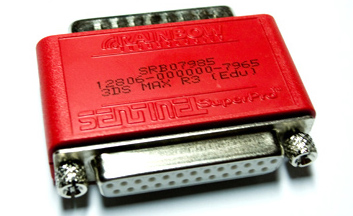
\includegraphics[width=0.5\textwidth]{superpro.jpg}
\end{figure}

In general, it is somewhat unlawful to break software protection, so I can do this only if these conditions are met:

	\begin{itemize}
	\item the software company who developed the software product does not exist anymore to my best knowledge;
	\item the software product is older than 10 years;
	\item you have a dongle to read information from it. In other words, I can only help to those who still uses some very old software, completely satisfied with it, but afraid of dongle electrical breakage and there are no company who can still sell the dongle replacement.
	\end{itemize}

These includes ancient MS-DOS and UNIX software. Software for exotic computer architectures (like MIPS, DEC Alpha, PowerPC) accepted as well.

Examples of my work you may find in this book.

Typical price is USD 300.

E-Mail: \EMAIL{}, Skype: dennis.yurichev, Telegram: \TT{@yurichev}.

}
%\DE{\include{1st_page_DE}}
%\ES{\include{1st_page_ES}}
%\CN{\include{1st_page_CN}}

\RU{\begin{titlepage}
\vspace*{\fill}

\begin{flushright}
\IT{Эта книга посвящается \\
компьютеру Intertec Superbrain II}
\end{flushright}

\vspace*{\fill}
\end{titlepage}

}
\EN{\begin{titlepage}
\vspace*{\fill}

\begin{flushright}
\IT{This book is dedicated to \\
Intertec Superbrain II computer}

\end{flushright}

\vspace*{\fill}
\end{titlepage}

}
\FR{\begin{titlepage}
\vspace*{\fill}

\begin{flushright}
\IT{Ce livre est dédié à \\
l'ordinateur Intertec Superbrain II}
\end{flushright}

\vspace*{\fill}
\end{titlepage}

}

\include{page_after_cover}
\include{call_for_translators}

\shorttoc{%
    \RU{Краткое оглавление}%
    \EN{Abridged contents}%
    \ES{Contenidos abreviados}%
    \PTBRph{}%
    \DE{Inhaltsverzeichnis (gekürzt)}%
    \PLph{}%
    \ITAph{}%
    \THAph{}\NLph{}%
    \FR{Contenus abrégés}%
    \JPN{簡略版}
}{0}

\tableofcontents
\cleardoublepage

\cleardoublepage
\include{preface}

\mainmatter

% only chapters here!
\ifdefined\SPANISH
\chapter{Patrones de código}
\fi % SPANISH

\ifdefined\GERMAN
\chapter{Code-Muster}
\fi % GERMAN

\ifdefined\ENGLISH
\chapter{Code Patterns}
\fi % ENGLISH

\ifdefined\ITALIAN
\chapter{Forme di codice}
\fi % ITALIAN

\ifdefined\RUSSIAN
\chapter{Образцы кода}
\fi % RUSSIAN

\ifdefined\BRAZILIAN
\chapter{Padrões de códigos}
\fi % BRAZILIAN

\ifdefined\THAI
\chapter{รูปแบบของโค้ด}
\fi % THAI

\ifdefined\FRENCH
\chapter{Pattern de code}%meilleur?
\fi % FRENCH

\ifdefined\POLISH
\chapter{\PLph{}}
\fi % POLISH

\ifdefined\JAPANESE
\chapter{コードパターン}
\fi % JAPANESE

\ifdefined\TURKISH
\chapter{Kod Şablonları}
\fi % Turkish

% sections
\EN{\mysection{The method}

When the author of this book first started learning C and, later, \Cpp, he used to write small pieces of code, compile them,
and then look at the assembly language output. This made it very easy for him to understand what was going on in the code that he had written.
\footnote{In fact, he still does this when he can't understand what a particular bit of code does.}.
He did this so many times that the relationship between the \CCpp code and what the compiler produced was imprinted deeply in his mind.
It's now easy for him to imagine instantly a rough outline of a C code's appearance and function.
Perhaps this technique could be helpful for others.

%There are a lot of examples for both x86/x64 and ARM.
%Those who already familiar with one of architectures, may freely skim over pages.

By the way, there is a great website where you can do the same, with various compilers, instead of installing them on your box.
You can use it as well: \url{https://godbolt.org/}.

\section*{\Exercises}

When the author of this book studied assembly language, he also often compiled small C functions and then rewrote
them gradually to assembly, trying to make their code as short as possible.
This probably is not worth doing in real-world scenarios today,
because it's hard to compete with the latest compilers in terms of efficiency. It is, however, a very good way to gain a better understanding of assembly.
Feel free, therefore, to take any assembly code from this book and try to make it shorter.
However, don't forget to test what you have written.

% rewrote to show that debug\release and optimisations levels are orthogonal concepts.
\section*{Optimization levels and debug information}

Source code can be compiled by different compilers with various optimization levels.
A typical compiler has about three such levels, where level zero means that optimization is completely disabled.
Optimization can also be targeted towards code size or code speed.
A non-optimizing compiler is faster and produces more understandable (albeit verbose) code,
whereas an optimizing compiler is slower and tries to produce code that runs faster (but is not necessarily more compact).
In addition to optimization levels, a compiler can include some debug information in the resulting file,
producing code that is easy to debug.
One of the important features of the ´debug' code is that it might contain links
between each line of the source code and its respective machine code address.
Optimizing compilers, on the other hand, tend to produce output where entire lines of source code
can be optimized away and thus not even be present in the resulting machine code.
Reverse engineers can encounter either version, simply because some developers turn on the compiler's optimization flags and others do not.
Because of this, we'll try to work on examples of both debug and release versions of the code featured in this book, wherever possible.

Sometimes some pretty ancient compilers are used in this book, in order to get the shortest (or simplest) possible code snippet.
}
\ES{\mysection{\ESph{}}

Cuando el autor de este libro comenzó a aprender C y, más tarde, \Cpp, él solía escribir pequeños trozos de código, compilarlos, 
y luego ver los resultados en lenguaje assembly. Esto lo hizo muy fácil para él entender lo que estaba pasando en el código que había escrito.
\footnote{De hecho, todavia lo hace cuando no puede entender lo que hace una determinada pieza de código.}. 
Él lo hizo tantas veces que la relación entre el código \CCpp y lo que el compilador producido se imprimió profundamente en su mente. 
És fácil imaginar al instante un esbozo de la aparencia y función del código C. 
Quizás esta técnica podría ser útil para otra persona.

%Hay una serie de ejemplos, tanto para x86/x64 y ARM.
%Los que ya están familiarizados con alguna de las arquitecturas, pueden leer superficialmente las páginas siguientes.

En ciertas partes, se han empleado aquí compiladores muy antiguas, con el fin de obtener lo mas corta (o simple) posible snippet.
\ac{TBT}.
\section*{\Exercises}

Cuando el autor de este libro estudió la lenguaje assembly, también con frecuencia compilaba pequeñas funciones en C, y reescribia gradualmente en assembly, tratando de hacer el código lo más pequeño posible.
Probablemente no vale la pena hacer esto en escenarios reales actualmente, 
porque es dificil competir con los compiladores modernos en términos de eficiencia. Es, sin embargo, una muy buena manera de obtener una mejor compreensión de la assembly.
Siéntase libre, por lo tanto, para tomar cualquier código de este libro y tratar de hacerlo más pequeño.
Sin embargo, no se olvide de probar lo que has escrito.

\section*{Níveles de optimización y la información de depuración}
El código fuente puede ser compilado por diferentes compiladores com varios niveles de optimización.
Un compilador típico tiene alredor de tres de esos niveles, donde el nivel cero significa desactivar la optimización.
La optimización también puede dirigirse hacia el tamaño del código o la velocidad de código.
Un compilador sin optimización es más rápido y produce código más inteligible (aunque más grande), 
mientras un compilador con optimización es más lento y trata de producir un código que corre más rápido (pero no necesariamente más compacto).
Además de los niveles y dirección de la otimización, el compilador puede incluir informaciones de depuración en el archivo resultante, produciendo así código para fácil depuración.
Una de los características importantes del código de ´debug' és que puede contener enlaces entre
cada línea del código fuente y las direcciones de código de máquina respectivos.
Compiladores con optimización, por otro lado, tienden a producir una salida donde líneas enteras de código fuente pueden ser optimizados al punto de ser eliminados y por consiguiente no estar presentes en el código de máquina resultante.
Ingenieros Inversos pueden encontrar ambas versiones, simplesmente porque alguns desarrolladores activan los flags de optimización del compilador, y otros no activan. 
Debido a esto, vamos a tratar de trabajar con ejemplos de ambas versiones de debug y release del código resaltado en este libro, cuando sea posible.

}
\ITA{\mysection{\ITAph{}}

Quando l'autore di questo libro ha cominciato ad imparare il C e, successivamente, \Cpp, era solito scrivere piccoli pezzi di codice, compilarli e guardare l'output prodotto in linguaggio assembly. Questo procedimento ha facilitato la comprensione del comportamento del codice che aveva scritto.

\footnote{In effetti lo fa ancora oggi quando non riesce a capire cosa fa un particolare pezzo di codice.}. 
Lo ha fatto talmente tante volte che la relazione tra il codice \CCpp e ciò che viene prodotto dal compilatore si è impressa profondamente nella sua mente. E' facile immaginare a colpo d'occhio un contorno della forma e della funzione di un dato codice C. 
Magari questa tecnica può rivelarsi utile anche per gli altri.

%There are a lot of examples for both x86/x64 and ARM.
%Those who already familiar with one of architectures, may freely skim over pages.

In queso libro sono talvolta utilizzati vecchi compilatori al fine di ottenere il frammento di codice più piccolo (o semplice) possibile.
\ac{TBT}.
\section*{\Exercises}

Quando l'autore di questo libro studiava il linguaggio assembly, era solito anche compilare piccola funzioni C e riscriverle gradualmente in assembly tentando di restringere il codice il più possibile.
Questa pratica è oggi probabilmente inutile in uno scenario reale, in quanto è molto difficile competere, in termini di efficienza, con i moderni compilatori. Rappresenta comunque un ottimo modo di acquisire una migliore conoscenza dell'assembly.
Sentitevi quindi liberi di prendere qualunque pezzo di codice assembly da questo libro e cercare di renderlo più piccolo. Tuttavia non dimenticate di testare il vostro risultato.

\section*{Livelli di ottimizzazione e informazioni di debug}

Il codice sorgente può essere compilato da compilatori diversi e con vari livelli di ottimizzazione.
Un compilatore tipico ne prevede solitamente tre, dei quali il livello zero corrisponde a nessuna ottimizzazione (ottimizzazione disabilitata) 

L'ottimizzazione può essere orientata verso la dimensione del codice o la sua velocità di esecuzione.
Un compilatore non ottimizzante è più veloce e produce codice più comprensibile (sebbene prolisso), mentre un compilatore ottimizzante è più lento e cerca di produrre codice più veloce in termini di performance (ma non necesariamente più compatto).
Oltre a livelli e direzione di ottimizzazione, un compilatore può includere informazioni di debug nel file risultante, producendo quindi codice che può essere debuggato più facilmente.
Una delle caratteristiche più importanti del codice di ´debug' è che può contenere collegamenti tra ogni riga del codice sorgente e l'indirizzo del corrispondente codice macchina.
I compilatori ottimizzanti tendono invece a produrre output in cui intere righe di codice sorgente possono essere ottimizzate a tal punto da non essere neanche presenti nel codice macchina risultante.
I reverse engineers possono incontrare entrambe le version, semplicemente perchè alcuni sviluppatori utilizzano le opzioni di ottimizzazione dei compilatori ed altri no. A causa di ciò negli esempi proveremo, quando possibile, a lavorare sia sulle versioni di debug che su quelle di release del codice illustrato in questo libro.
}
\PTBR{\mysection{\PTBRph{}}

Quando o autor desse livro começou a aprender C e depois C++, ele costumava escrever pequenos pedaços de código, compilar e entã o olhar na sua saída em assembly.
Isso acabou tornando muito fácil para o seu entendimento sobre o que estava acontecendo no código que ele escreveu.
Ele fez isso tantas vezes, que a relação entre o código em \CCpp e o que o compilador produzia ficou gravada em sua mente.
É facil imaginar a aparência e função de um rascunho em C. Algumas vezes essa técnica pode ser útil para outras pessoas.

Ás vezes compiladores antigos serão usados aqui com o objetivo de conseguir o menor (ou mais simples) pedaço de código possível.

\iffalse
% other version...
Quando o autor deste livro começou a aprender C e, mais tarde, \Cpp, ele costumava escrever pequenos pedaços de código, compilá-los, 
e então olhar a saída em linguagem assembly. Isso tornou muito fácil para ele entender o que estava acontecendo no código que ele tinha escrito.
\footnote{Na verdade, ele ainda faz isso quando não consegue entender o que faz um determinado pedaço de código.}. 
Ele fez isso tantas vezes que o relacionamento entre o código \CCpp code e o que o compilador produzia ficou registrado profundamente em sua mente. 
É fácil imaginar de imediato um esboço da aparência e função do código C. 
Talvez essa técnica poderia ser útil para mais alguém.

%Há uma série de exemplos para ambos x86/x64 e ARM.
%Aqueles já familiarizados com alguma das arquiteturas, pode ler superficialmente as próximas páginas.

Em determinadas partes foram usados aqui compiladores muito antigos, para se obter o menor (ou mais simples) snippet possível.
\fi
\ac{TBT}.
\section*{\Exercises}

Quando o autor deste livro estudou a linguagem assembly, ele também frequentemente compilava pequenas funções em C e então as reescrevia gradualmente em assembly, tentando fazer seu código o menor possível.
Provavelmente não vale mais à pena fazer isso em cenários reais atualmente, 
porque é difícil competir com os compiladores modernos em termos de eficiência. É, no entanto, uma forma muito boa de obter um melhor entendimento de assembly.
Sinta-se livre, portanto, para pegar qualquer código assembly deste livro e tentar torná-lo menor.
No entanto, não esqueça de testar o que você tiver escrito.

\section*{Níveis de otimização e informações de depuração}

O código-fonte pode ser compilado por um número diferente de compiladores com vários níveis de otimização.
Um compilador típico tem por volta de três desses níveis, onde o nível zero representa que a otimização está desabilitada.
A otimização também pode ser relacionada com o tamanho ou velocidade do código.
Um compilador não-otimizado é mais rápido e produz um código de mais fácil compreensão (embora detalhado),
enquanto um compilador com otimização é mais lento e tenta produzir códigos que executam mais rápido (mas não necessariamente mais compactos).
Em adição aos níveis de otimização e  direção, um compilador pode incluir no arquivo de saída algumas informações de depuração, dessa maneira produzindo código para fácil depuração.
Uma das características de um código ``depurado'' é que ele pode conter ligações entre cada linha do código-fonte e o endereço do respectivo código de máquina.
Compiladores otimizadores, por outro lado, tendem a produzir saídas onde linhas completas do código-fonte podem ser otimizadas e apresentadas de uma maneira completamente diferente,
muitas vezes ainda nem estando presente no código de máquina resultate. Com a engenharia reversa podemos obter quaisquer versões,
simplesmente porque alguns desenvolvedores ativam as otimizações do compilador e outros não.
Por causa disso, nós tentaremos trabalhar em ambos exemplos de depuração e versões de lançamento dos códigos demonstrados nesse livro, quando possível.

\iffalse
% another version
\section*{Níveis de otimização e informação de depuração}

O código-fonte pode ser compilado por diferentes compiladores com vários níveis de otimização.
Um compilador típico tem cerca de três destes níveis, onde o nível zero significa desativar a otimização.
A otimização também pode ser direcionada para o tamanho do código ou para a velocidade do código.
Um compilador sem otimização é mais rápido e produz código mais inteligível (embora maior),
enquanto que um compilador com otimização é mais lento e tenta produzir um código que execute mais rápido (mas não é necessariamente mais compacto).
Além dos níveis e direcionamento da otimização, o compilador pode incluir no arquivo resultante algumas informações de depuração, produzindo assim código para fácil depuração.
Uma das características importantes do código de ´debug' é que ele pode conter 
ligações entre cada linha do código-fonte e os respectivos endereços de código de máquina.
Compiladores com otimização, por outro lado, tendem a produzir uma saída onde linhas inteiras de código-fonte podem ser otimizadas a ponto de serem removidas e portanto não estarem presentes no código de máquina resultante.
Engenheiros Reversos podem encontrar ambas as versões, simplesmente porque alguns desenvolvedores ativam as flags de otimização do compilador e outros não ativam. 
Por causa disso, nós tentaremos trabalhar em exemplos de ambas as versões de debug e release do código destacado neste livro, onde possível.
\fi
}
\RU{\mysection{Метод}

Когда автор этой книги учил Си, а затем \Cpp, он просто писал небольшие фрагменты кода, компилировал и смотрел, что 
получилось на ассемблере. Так было намного проще понять%
\footnote{Честно говоря, он и до сих пор так делает, когда не понимает, как работает некий код.}.
Он делал это такое количество раз, что связь между кодом на \CCpp и тем, что генерирует компилятор, вбилась в его подсознание достаточно глубоко.
После этого не трудно, глядя на код на ассемблере, сразу в общих чертах понимать, что там было написано на Си. 
Возможно это поможет кому-то ещё.

%Здесь много примеров и для x86/x64 и для ARM.
%Те, кто уже хорошо знаком с одной из архитектур, могут легко пролистывать страницы.

Иногда здесь используются достаточно древние компиляторы, чтобы получить самый короткий (или простой) фрагмент кода.

Кстати, есть очень неплохой вебсайт где можно делать всё то же самое, с разными компиляторами, вместо того чтобы инсталлировать
их у себя.
Вы можете использовать и его: \url{http://godbolt.org/}.

\section*{\Exercises}

Когда автор этой книги учил ассемблер, он также часто компилировал короткие функции на Си и затем постепенно 
переписывал их на ассемблер, с целью получить как можно более короткий код.
Наверное, этим не стоит заниматься в наше время на практике (потому что конкурировать с современными
компиляторами в плане эффективности очень трудно), но это очень хороший способ разобраться в ассемблере
лучше.
Так что вы можете взять любой фрагмент кода на ассемблере в этой книге и постараться сделать его короче.
Но не забывайте о тестировании своих результатов.

\section*{Уровни оптимизации и отладочная информация}

Исходный код можно компилировать различными компиляторами с различными уровнями оптимизации.
В типичном компиляторе этих уровней около трёх, где нулевой уровень~--- отключить оптимизацию.
Различают также уровни оптимизации кода по размеру и по скорости.
Неоптимизирующий компилятор работает быстрее, генерирует более понятный (хотя и более объемный) код.
Оптимизирующий компилятор работает медленнее и старается сгенерировать более быстрый (хотя и не обязательно краткий) код.
Наряду с уровнями оптимизации компилятор может включать в конечный файл отладочную информацию,
производя таким образом код, который легче отлаживать.
Одна очень важная черта отладочного кода в том, что он может содержать
связи между каждой строкой в исходном коде и адресом в машинном коде.
Оптимизирующие компиляторы обычно генерируют код, где целые строки из исходного кода
могут быть оптимизированы и не присутствовать в итоговом машинном коде.
Практикующий reverse engineer обычно сталкивается с обеими версиями, потому что некоторые разработчики
включают оптимизацию, некоторые другие --- нет. Вот почему мы постараемся поработать с примерами для обеих версий.
}
\THA{\mysection{\THAph{}}

เมื่อครั้งที่ผู้แต่งหนังสือเริ่มต้นเรียนรู้ภาษา C และในเวลาถัดมา C++ เขาเคยเขียนโค้ดสั้น ๆ และทำการคอมไพล์ แล้วสังเกตดูผลลัพธ์ที่ได้จากการคอมไพล์ที่เป็นภาษาแอสแซมบลี ซึ่งช่วยให้เข้าใจได้ง่ายขึ้นว่าโค้ดที่เขียนนั้นมีการทำงานอย่างไร เขาทำแบบนั้นอยู่หลายครั้งจนความสัมพันธ์ระหว่างโค้ดภาษา C/C++ กับผลลัพธ์ที่ได้จากการคอมไพล์ประทับอยู่ในจิตใจ มันเป็นการง่ายมากที่จะนึกถึงถึงรูปร่างและฟังก์ชั่นของโค้ดภาษา C ขึ้นมาทันที บางครั้งเทคนิคนี้อาจจะมีประโยชน์กับคนอื่นก็ได้	
% rough translation (using google) of the text above: "When the author started learning C and C ++ in the next period, he had written a short code and compile. Then see the results of the compilation of the Assembly's language. This allows more easily understand what the code is written work, however. He did that several times the relationship between the code language C / C ++ with the results from the compilation is in the mind. It's very easy to think of the shape and function of the C language code immediately, sometimes this technique could be useful to someone else."

% To be continued...

}
\DE{\mysection{Die Methode}

Als der Autor dieses Buches zunächst C und später \Cpp lernte, schrieb er kleine Codestücke, kompilierte sie und
untersuchte anschließend den Assembler-Code des Compilers. Dies machte es sehr einfach zu verstehen, was in dem Code
den er geschrieben hatte passierte.
\footnote{Tatsächlich tut er dies immer noch wenn er einen bestimmten Code-Teil nicht versteht.} 
Er hat dies so oft getan, dass der Zusammenhang zwischen dem \CCpp-Code und dem was der Compiler daraus macht tief in
seinem Verstand verankert ist. % Not very elegant translation to be honest... 
So ist es einfach sich schnell einen Überblick über das Aussehen und die Funktion einer C-Quelle zu verschaffen. 
Vielleicht ist diese Vorgehensweise auch für andere hilfreich.

%There are a lot of examples for both x86/x64 and ARM.
%Those who already familiar with one of architectures, may freely skim over pages.

Übrigens gibt es eine hervorragende Webseite auf der dasselbe mit verschiedenen
Compilern getan werden kann, anstatt diese zu installieren.
Auch diese kann genutzt werden: \url{https://godbolt.org/}.

\section*{\Exercises}

Als der Autor dieses Buches Assembler erlernte, hat er oft kleine C-Funktionen kompiliert und anschließend nach und nach in
Assembler nachprogrammiert um den Code so klein wie möglich zu machen.
Dies ist in einer Anwendung in der Praxis heutzutage vielleicht nicht mehr sinnvoll, weil moderne Compiler in der Regel weitaus
besser optimieren können als ein Mensch. Dennoch ist es ein guter Weg um Assembler besser zu verstehen. Versuchen Sie ruhig
einmal einen Assembler-Quelltext aus dem Buch bei gleicher Funktionalität kürzer zu schreiben.
Vergessen Sie aber nicht Dinge die Sie programmiert haben zu testen.

% rewrote to show that debug\release and optimisations levels are orthogonal concepts.
\section*{Optimierungsstufen und Debug-Informationen}

Quellcode kann von verschiedenen Compilern mit verschiedenen Optimierungsstufen übersetzt werden.
Üblicherweise hat ein Compiler drei solcher Stufen, wobei Stufe Null eine deaktivierte Optimierung bedeutet.
Die Optimierung kann sich ebenso auf die Code-Größe als auch auf die Ausführgeschwindigkeit beziehen.
Ein Nicht-optimierender Compiler ist schneller und erstellt einfacher zu verstehenden (aber auch längeren) Code.
Demgegenüber ist ein optimierender Compiler langsamer und versucht Code zu erstellen, dessen Ausführgeschwindigkeit
höher, aber nicht notwendigerweise kompakter, ist.
Zusätzlich zu diesen Optimierungsmöglichkeiten kann ein Compiler Informationen in den Code einfügen, die das spätere
Debuggen vereinfachen.
Eine wichtige Eigenschaft des Debug-Codes ist, dass er gegebenenfalls Links zwischen den Zeilen des Quellcodes und
den entsprechenden Maschinen-Code-Adressen enthält.
Optimierende Compiler hingegen tendieren dazu Code zu erzeugen, der ganze Zeilen des Quellcodes wegoptimiert, die dann
dementsprechend im Maschinencode nicht auftauchen.
Ein Reverse Engineer kann beiden Varianten begegnen, einfach, weil einige Software-Entwickler die Optimierung des Compilers
nutzen und andere nicht. Aufgrund dieser Tatsache werden Sie in diesem Buch auch Beispielcode für optimierten und
nichtoptimierten Compiler-Code finden.
}
\FR{\mysection{La méthode}

Lorsque l'auteur de ce livre a commencé à apprendre le C, et plus tard, le \Cpp, il a pris l'habitude d'écrire des petits morceaux de
code, de les compiler et de regarder le langage d'assemblage généré.
Cela lui a permis de comprendre facilement ce qui se passe dans le code qu'il écrit.
\footnote{En fait, il fait encore cela lorsqu'il ne comprend pas ce qu'un morceau de code fait.}
Il l'a fait si souvent que la relation entre le code \Cpp et ce que le compilateur produit a été imprimée profondément dans son
 esprit.
Ça lui est facile d'imaginer immédiatement l'allure de la fonction et du code C.
Peut-être que cette méthode pourrait être utile à d'autres.

%Il y a beaucoup d'exemples pour x86/x64 et ARM.
%Ceux qui sont déjà familier avec l'une de ces architectures peuvent rapidement survoler ces pages.

Parfois, des anciens compilateurs sont utilisés, afin d'obtenir des extraits de code le plus court (ou le plus simple) possible.

À propos, il y a un bon site où vous pouvez faire la même chose, avec de nombreux
compilateurs, au lieu de les installer sur votre système.
Vous pouvez également l'utiliser: \url{https://godbolt.org/}.

\section*{\Exercises}

Lorsque l'auteur de ce livre étudiait le langage d'assemblage, il a souvent compilé des petites fonctions en C et les a ensuite
récrites peu à peu en assembleur, en essayant d'obtenir un code aussi concis que possible.
Cela n'en vaut probablement plus la peine aujourd'hui, car il est difficile
de se mesurer aux derniers compilateurs en terme d'efficacité. Cela reste par contre un excellent moyen d'approfondir ses connaissances
de l'assembleur.
N'hésitez pas à prendre n'importe quel code assembleur de ce livre et à essayer de le rendre plus court.
Toutefois, n'oubliez pas de tester ce que vous aurez écrit.

\section*{Niveau d'optimisation et information de débogage}

Le code source peut être compilé par différents compilateurs, avec des niveaux d'optimisation variés.
Un compilateur en a typiquement trois, où le niveau 0 désactive l'optimisation.
L'optimisation peut se faire en ciblant la taille du code ou la vitesse d'exécution.
Un compilateur sans optimisation est plus rapide et produit un code plus compréhensible (quoique verbeux),
alors qu'un compilateur avec optimisation est plus lent et essaye de produire un code qui s'exécute plus
vite (mais pas forcément plus compact).
En plus des niveaux d'optimisation, un compilateur peut inclure dans le fichier généré des informations de
débogage, qui produit un code facilitant le débogage.
Une des caractéristiques importante du code de 'debug', est qu'il peut contenir des liens entre chaque ligne du code source et
les adresses du code machine associé.
D'un autre côté, l'optimisation des compilateurs tend à générer du code où des lignes du code source sont modifiées, et
même parfois absentes du code machine résultant.
Les rétro-ingénieurs peuvent rencontrer n'importe quelle version, simplement parce que certains développeurs mettent les options
d'optimisation, et d'autres pas.
Pour cette raison, et lorsque c'est possible, nous allons essayer de travailler sur des exemples avec les versions de débogage
et finale du code présenté dans ce livre.
}
\PL{\mysection{Metodyka}

Kiedy autor tej książki uczył się C, a później \Cpp, pisał tylko niewielkie kawałki kodu, kompilował i patrzył jak wyglądają w assemblerze. Tak było o wiele łatwiej zrozumieć co się dzieje w programie.%
\footnote{Szczerze mówiąc, dalej tak robi, kiedy nie rozumie jak jakiś kod działa.}.
Robił to wystarczająco dużą ilość razy, żeby związek między kodem w \CCpp a tym co generuje kompilator wbił się w jego podświadomość bardzo głęboko. Po tym, patrząc na kod w assemblerze, od razu ogólnikowo rozumiał to co było napisane w C. Możliwe, że to pomoże komuś jeszcze.

%Tu jest dużo przykładów do x86/x64 zarówno jak i do ARM.
%Ci którzy są wystarczająco dobrze obeznani z jedną z architektur, mogą pomijać te fragmenty.

Czasami będą wykorzystywane stare kompilatory, żeby otrzymać bardzo krótki lub prosty kawałek kodu.

A propos, jest jedna dobra strona, gdzie można robić wszystko to samo z różnymi kompilatorami bez konieczności instalowania ich u siebie: \url{http://godbolt.org/}.

\section*{\Exercises}

Kiedy autor tej książki uczył się assemblera, on również często kompilował krótkie funkcje w C i powoli przepisywał je na assembler, mając na celu otrzymanie jak najkrótszego kodu. Możliwe, że nie jest to obecnie niezbędne jako że współczesne kompilatory optymalizują kod najbardziej jak się da, ale jest to bardzo dobry sposób, żeby oswoić się z assemblerem. Także możecie wziąć dowolny fragment kodu w assemblerze z tej książki i postarać się zrobić go krótszym. Warto nie zapominać o testowaniu wyników.

\section*{Poziomy optymalizajci i debuggowanie}

Kod źródłowy można kompilować różnymi kompilatorami z różnym poziomami optymalizacji. W typowym kompilatorze jest tych poziomów około trzech, gdzie poziom zerowy oznacza wyłączoną optymalizację. Rozróżnia się także kierunki optymalizacji według rozmiaru i poziomu prędkości. Niezoptymalizujący kompilator działa szybciej i generuje bardziej przejrzysty kod (choć i większy objętościowo). Optymalizujący kompilator działa wolniej i stara się wygenerować jak najszybszy kod (co nie zawsze znaczy, że kod będzie krótszy). Obok poziomów i kierunków optymalizacji kompilator może załączać do pliku wyniki debuggowania, tworząc w ten sposób kod, który jest prostszy w debuggowaniu. Bardzo ważną cechą kodu debuggowanego jest to, że zawiera on związki między każdą linią kodu źródłowego i adresem w kodzie maszynowym. Optymalizujące kompilatory zwykle generują kod, gdzie całe linie kodu źródłowego mogą zostać pominięte. Praktykujący reverse engineer z reguły ma styczność z obiema wersjami, jako że niektórzy developerzy włączają optymalizację, a niektórzy - nie. Dlatego postaramy się ćwiczyć rozważając obie możliwości.

}
\JPN{\mysection{方法}

この本の著者はC言語、その後Cppを学び始めたとき、小さなコードを書いてコンパイルし、アセンブリ言語の出力を見ていました。 これにより、彼が書いたコードで何が起こっているのかを理解することが非常に容易になりました。\footnote{実際、彼はコードの特定のビットが何をしているのか理解できないときもこれを実行します}
彼はこれを何度もやって、Cppコードとコンパイラが作り出したものとの関係が彼の心の中に深く刻まれていたことを知っています。 今では、Cコードの外観と機能の概要を即座に想像するのは簡単です。 おそらく、このテクニックは他の人に役立つかもしれません。

%There are a lot of examples for both x86/x64 and ARM.
%Those who already familiar with one of architectures, may freely skim over pages.

なお、PCにインストールせずに、さまざまなコンパイラを使ってPCと同じことができる素晴らしいWebサイトがあります。あなたもそれを使うことができます:\url{https://godbolt.org/}

\section*{練習問題}

この本の作者がアセンブリ言語を学んだとき、彼はしばしば小さなC関数をコンパイルしてから、
アセンブリを徐々に書き直してコードを可能な限り短くしようとしました。 効率性の点で最新のコンパイラと競争するのは難しいため、
現実のシナリオではこれはおそらく価値がありません。 しかし、それはアセンブリのより良い理解を得るための非常に良い方法です。 
したがって、この本の中からアセンブリコードを取り出して短くしてみてください。 
しかし、あなたが書いたものをテストすることを忘れないでください。

% rewrote to show that debug\release and optimisations levels are orthogonal concepts.
\section*{最適化レベルとデバッグ情報}

ソースコードはさまざまな最適化レベルを持つ異なるコンパイラによってコンパイルできます。
典型的なコンパイラにはこのようなレベルが約3つあります。レベル0は最適化が完全に無効になっていることを意味します。
最適化は、コードサイズやコードの速度に合わせることもできます。最適化されていないコンパイラはより高速でより理解しやすいコードを生成しますが、
最適化コンパイラは遅くなり、実行速度の速いコードを生成しようとします(コンパクトである必要はありません)。
最適化レベルに加えて、コンパイラは結果ファイルにいくつかのデバッグ情報を含めて、デバッグしやすいコードを生成することができます。
「デバッグ」コードの重要な機能の1つは、ソースコードの各行とそれぞれのマシンコードアドレスとの間にリンクを含む可能性があることです。
一方、コンパイラを最適化すると、ソースコードの行全体が最適化され、結果のマシンコードにも存在しない出力が生成される傾向があります。
リバースエンジニアはいずれかのバージョンに遭遇する可能性があります。
なぜなら、一部の開発者はコンパイラの最適化フラグをオンにし、他の開発者はそうしないからですこのため、
可能であれば、本書に記載されているコードのデバッグ版とリリース版の両方の例を取り上げようとします。

最も短い(または最も単純な)コードスニペットを得るために、時にはかなり古いコンパイラがこの本で使われています。
}

\RU{\mysection{Некоторые базовые понятия}}
\EN{\mysection{Some basics}}
\DE{\mysection{Einige Grundlagen}}
\FR{\mysection{Quelques bases}}
\ES{\mysection{Algunos conceptos basicos}}
\ITA{\mysection{Alcune basi teoriche}}
\PTBR{\mysection{\PTBRph{}}}
\THA{\mysection{\THAph{}}}
\PL{\mysection{\PLph{}}}
\TR{\mysection{Temeller}}
\JPN{\mysection{基本的な事柄}}

% sections:
\EN{\input{patterns/intro_CPU_ISA_EN}}
\ES{\input{patterns/intro_CPU_ISA_ES}}
\ITA{\mysection{Una breve introduzione alla CPU}

La \ac{CPU} è il dispositivo che esegue il codice macchina di cui è fatto un programma.

\textbf{Un breve glossario:}

\begin{description}
\item[Istruzione]: Un comando \ac{CPU} primitivo.
L'esempio piò semplice include: spostare dati da un registro all'altro, lavorare con la memoria, effettuare operazioni aritmetiche primitive.
Di norma ogni \ac{CPU} ha il suo insieme di istruzioni, detto instruction set architecture o (\ac{ISA}).

\item[Codice macchina]: Codice che la \ac{CPU} è in grado di processare direttamente. 
Ciascuna istruzione è solitamente codificata da diversi byte.
\item[Linguaggio Assembly]: Codici mnemonico ed alcune estensioni come le macro introdotti per facilitare la vita del programmatore.
\item[Registro CPU]: Ogni \ac{CPU} ha un insieme finito di registri generici (\ac{GPR}).
$\approx 8$ in x86, $\approx 16$ in x86-64, $\approx 16$ in ARM.
Il modo più semplice per capire un registro è quello di pensare ad esso come una variabile temporanea senza tipo.
Immagina se stessi lavorando con un linguaggio di programmazione di alto livello \ac{PL} e potessi usare solo otto variabili a 32 (o 64) bit.

Eppure solo con questi si possono fare un sacco!
\end{description}

% TODO1 add about linker: "компоновщик" и "редактор связей" в русскоязычной лит-ре

% A note on the experiments in this area (like the LISP machines http://en.wikipedia.org/wiki/Lisp_machine
% might be useful
Qualcuno potrebbe chiedersi perchè ci debba essere una differenza tra il codice macchina ed un ac{PL}. La risposta risiede nel fatto che gli umani e i processori (\ac{CPU}) non sono uguali---%
per un umano è molto più facille utilizzare un linguaggio di programmazione ad alto livello come \CCpp, Java, Python, etc., mentre per una \ac{CPU} è più semplice utilizzare un livello di astrazione più basso.
Potrebbe essere forse possibile inventare una \ac{CPU} in grado di eseguire codice di un linguaggio \ac{PL} ad alto livello, ma sarebbe molto più complesso dei processori che conosciamo oggi.
Allo stesso modo sarebbe del tutto sconveniente per gli umani scrivere in linguaggio assembly, a causa della sua natura di basso livello e la difficoltà nello scrivere senza commettere un enorme numero di fastidiosi errori.
Il programma che converte il codice di un \ac{PL} di alto livello in assembly è detto un \IT{compilatore}.
\footnote{La vecchia letteratura russa in materia utilizza il termine \q{traduttore}.}.

\myindex{ARM!\ARMMode}%
\myindex{ARM!\ThumbMode}%
\myindex{ARM!\ThumbTwoMode}%

\subsection{Qualche parola sulle diverse \ac{ISA}}
L'architettura x86 \ac{ISA} è sempre stata una con opcodes di lunghezza variabile, e all'arrivo dell'era 64-bit l'estensione x64 non ha avuto impatti significativi sulla \ac{ISA}. Infatti l'architettura x86 contiene molte istruzioni apparse per la prima volta nelle CPU a 16-bit 8086 che si trovano ancora nei processori odierni.
ARM è una \ac{CPU} \ac{RISC} progettata con opcodes di lunghezza costante, che in passato avevano alcuni vantaggi.
Originariamente tutte le istruzioni ARM erano codificate in 4 byte%
\footnote{
A proposito, le istruzioni a lunghezza fissa sono utili perchè è possibile calcolare senza sforzo l'indirizzo della prossiama (o della precedente) istruzione. Questa caratteristica sarà discussa nella sezione dedicata all'operatore switch() operator~(\myref{sec:SwitchARMLot}) .
}.
Oggi è noto come \q{ARM mode}.
Successivamente si pensò che non fosse poi tanto economico come si immaginava inizialmente.
Infatti, le istruzioni \ac{CPU} più usate \footnote{Che sono MOV/PUSH/CALL/Jcc} , in applicazioni reali, possono essere codificate usando meno informazioni.
Venne quindi aggiunta un'altra \ac{ISA}, detta Thumb, in cui ogni istruzione era codificata in solo 2 byte.
Oggi detto \q{Thumb mode}.
Tuttavia non \IT{tutte} le istruzioni ARM possono essere codificate in 2 byte, e il set di istruzioni Thumb è quindi in qualche modo limitato.
Vale la pena notare che il codice compilato in ARM mode e Thumb mode può tranquillamente coesistere all'interno dello stesso programma.
I creatori di ARM pensarono di estendere Thumb, dando vita a Thumb-2, appartso per la prima volta in ARMv7.
Thumb-2 utilizza ancora istruzioni da 2-byte, ma ha anche alcune nuove istruzioni da 4 byte. 

Esiste la convinzione errata che Thumb-2 sia un mix di ARM e Thumb. Questo non è corretto. 
Thumb-2 è stato invece esteso per supportare completamente tutte le caratteristiche del processore così da competere con l'ARM mode--- un goal che è stato chiaramente raggiunto, visto che la maggior parte delle applicazioni per \idevices sono compilate per il set di istruzioni Thumb-2 (in effetti, molto probabilmente dovuto anche al fatto che Xcode lo fa per default).
Successivamente fu la volta di ARM a 64-bit. Questa \ac{ISA} ha opcode di 4-byte, e non necessita di alcun Thumb mode aggiuntivo.
Tuttavia i requisiti a 64-bit hanno avuto un impatto sulla \ac{ISA}, motivo per cui abbiamo oggi tre set di istruzioni ARM: ARM mode, Thumb mode (incluso Thumb-2) e ARM64.
Queste \ac{ISA} si intersecano parzialmente, ma si può dire che sono \ac{ISA} differenti piuttosto che varianti della stessa.
Per questo motivo cercheremo di aggiungere frammenti di codice in tutte e tre le \ac{ISA} ARM in questo libro.
\myindex{PowerPC}%
\myindex{MIPS}%
\myindex{Alpha AXP}%
A proposito, esistono anche molte altre \ac{ISA}s \ac{RISC} con opcode a lunghezza fissa di 32-bit, come MIPS, PowerPC e Alpha AXP.
}
\PTBR{\input{patterns/intro_CPU_ISA_PTBR}}
\RU{\input{patterns/intro_CPU_ISA_RU}}
\DE{\input{patterns/intro_CPU_ISA_DE}}
\FR{\input{patterns/intro_CPU_ISA_FR}}
\PL{\subsection{Krótkie wprowadzenie do CPU}

\ac{CPU} (mikroprocesor) jest urządzeniem, które wykonuje bezpośrednio kod maszynowy programu.

\textbf{Terminologia:}

\begin{description}
\item[Instrukcja]: prymitywny rozkaz \ac{CPU}.
Najprostsze przykłady: przenoszenie (kopiowanie) danych między rejestrami, zarządzanie pamięcią, proste operacje arytmetyczne. 

Z reguły, każdy \ac{CPU} ma swój zestaw instrukcji (\ac{ISA}).

\item[Kod maszynowy]: kod wykonywany bezpośrednio przez \ac{CPU}. 
Każda instrukcja kodu maszynowego zwykle jest kodowana za pomocą kilku bajtów.
\item[Język asemblera]: kod maszynowy plus niektóre rozszerzenia (np. makra), stworzone po to, żeby ułatwić pracę programiście.
\item[Rejestr CPU]: Każdy \ac{CPU} ma swój zestaw rejestrów ogólnego przeznaczenia (\ac{GPR}).
$\approx 8$ w x86, $\approx 16$ w x86-64, $\approx 16$ w ARM.
Najłatwiej traktować rejestr jako zmienną bez określonego typu - wyobraź sobie, że pisząc w języku wyższego poziomu masz dostępne tylko 8 zmiennych o szerokości 32 (lub 64) bity. Te 8 zmiennych to właśnie rejestry. Wbrew pozorom można z nimi naprawdę wiele zrobić!
\end{description}

Dlaczego występują języki niższego i wyższego poziomu? Odpowiedź jest prosta: ludzie i procesory różnią się między sobą - dla człowieka jest o wiele łatwiej pisać w wysokopoziomowym języku programowania typu \CCpp, Java, Python, а dla procesora łatwiej jest pracować na niższym poziomie abstrakcji, ponieważ "rozumie" tylko kilkubajtowe instrukcje.
Możnaby zbudować procesor, który wykonywałby kod wysokiego poziomu, ale jego budowa byłaby dużo bardziej skomplikowana niż  budowa procesorów jakie obecnie znamy. 
\myindex{ARM!\ARMMode}%
\myindex{ARM!\ThumbMode}%
\myindex{ARM!\ThumbTwoMode}%

\subsubsection{Kilka słów o różnicy między \ac{ISA}}
x86 od zawsze  zawierał instrukcje o różnej długości, więc kiedy nadeszła era 64-bitowej architektury, rozszerzenia x64 nie wpłynęły znacząco na \ac{ISA}. 
ARM to \ac{RISC}- procesor zaprojektowany tak, żeby zawierał wszystkie instrukcje tej samej długości, co miało sporo zalet w przeszłosci. Na samym początku wszystkie instrukcje ARM były kodowane na czterech bajtach (obecnie \q{tryb ARM})%
\footnote{
Instrukcje o stałym rozmiarze są wygodne, bo dzięki temu można łatwo znaleźć adres następnej (lub poprzedniej) instrukcji. Dokładniejsze wyjaśnienie znajduje się w sekcji o operatorze switch()~(\myref{sec:SwitchARMLot}).
}.
Później się okazało, że jednak nie jest to zbyt wydajne, bo najczęściej używane przez procesor instrukcje\footnote{Są nimi MOV/PUSH/CALL/Jcc} mogą być zakodowane z wykorzystaniem mniejszej ilości informacji. Więc dodano inną \ac{ISA} o nazwie "Thumb", gdzie każda instrukcja jest kodowana za pomocą tylko 2 bajtów. Obecnie ta metoda jest nazywana \q{tryb Thumb}.
Jednak nie wszystkie instrukcje ARM mogą być zakodowane na 2 bajtach, także zestaw instrukcji Thumb jest ograniczony. Kod skompilowany dla trybu ARM i Thumb może współdziałać w jednym programie. Później producenci ARM stwierdzili, że Thumb można poszerzyć: tak się pojawił Thumb-2 (w ARMv7). Thumb-2 to wciąż dwubajtowe instrukcje, ale niektóre nowe instrukcje mają długość 4 bajtów. Szeroko rozpowszechnioną i błędną opinią jest to, że Thumb-2 to mieszanina ARM i Thumb. Tryb Thumb-2 był dopełniony, żeby lepiej wykorzystywać możliwości procesora i jest poważnym konkurentem trybu ARM. Aplikacje dla \idevices są głównie skompilowane dla zestawu instrukcji Thumb-2, ponieważ Xcode jest domyślnie skonfigurowane dla tego zestawu instrukcji. Później pojawił się 64-bitowy ARM. Jest to \ac{ISA} znowu z 4-bajtowymi instrukcjami, bez dodatkowego trybu Thumb. Jednak nowe 64-bitowe wymagania wpłyneły na \ac{ISA} tak, że obecnie mamy 3 zestawy instrukcji ARM: tryb ARM, tryb Thumb/Thumb-2 i ARM64. Te zestawy instrukcji gdzieniegdzie są podobne, ale można powiedzieć, że są to różne zestawy. W tej książce postaramy się zaprezentować fragmenty kodu we wszystkich trzech ARM  \ac{ISA}.
\myindex{PowerPC}%
\myindex{MIPS}%
\myindex{Alpha AXP}%
Istnieje jeszcze wiele \ac{RISC} \ac{ISA} z instrukcjami 32-bitowej długości~--- np. MIPS, PowerPC и Alpha AXP.

}
\JPN{\input{patterns/intro_CPU_ISA_JPN}}
\TR{\subsection{CPU'ya Giriş}

\ac{CPU} makine kodundan oluşan programları çalıştıran donanımdır. 

\textbf{Ufak bir Sözlük:}

\begin{description}
\item[Instruction]: İlkel bir \ac{CPU} komutu.
Basit bir örnek olarak: register (yazmaçlar) arasında değer taşıma, bellek ile çalışma, ilkel aritmetik operasyonlar verilebilir.
Genellikle, her \ac{CPU}'nun kendine has instruction listesi vardır (\ac{ISA}).

\item[Machine code]: \ac{CPU}'nun direkt olarak işleyebildiği kod.
Her instruction genellikle bir kaç byte ile gösterilir.
\item[Assembly language]: Programcının hayatını kolaylaştırmak için mnemonic kodlar ve bazı eklentiler (çeşitli microlar gibi) içeren bir dildir.
\item[CPU register]: Her \ac{CPU} sabit sayıda genel amaçlı register'dan (yazmaç) oluşur (\ac{GPR}).
x86'da $\approx 8$, x86-64'de $\approx 16$ ve ARM'da $\approx 16$ adet vardır.
Register'ları anlamanın en kolay yolu onları belirli bir tipi olmayan geçici değişkenler olarak düşünmektir.
Yüksek seviyeli bir \ac{PL} kullandığınızı ve yalnızca 32-bit (ya da 64-bit) değişkenler kullanabildiğinizi hayal edin.
Buna rağmen bir çok şeyi yapabilirdiniz!
\end{description}

% TODO1 add about linker: "компоновщик" и "редактор связей" в русскоязычной лит-ре

% A note on the experiments in this area (like the LISP machines http://en.wikipedia.org/wiki/Lisp_machine
% might be useful
Makine kodu ile bir \ac{PL} arasında neden fark olduğunu merak edebilirsiniz. Cevap insan beyninin ve \ac{CPU}'ların benzer çalışmadığında yatıyor.---%
İnsanlar için \CCpp, Java, or Python, gibi yüksek-seviyeli \ac{PL}'leri algılamaları daha kolay olmasına karşın \ac{CPU}'ler daha alçak-seviyeli soyutlamaları algılayabiliyor.
Muhtemelen \ac{CPU}'nun algılayabileceği yüksek-seviyeli bir dil icat etmek mümkün ama o zaman kullanılacak \ac{CPU}'ler günümüzdekilerden çok daha karmaşık olurlardı. 
Benzer olarak insanların düşük seviyeli bir dil olan assembly'de program yazması can sıkıcı hatalar ve buglar olmadan pek mümkün değil.
Yüksek seviyeli bir \ac{PL}'den assembly'e çevirme işlemini yapan programlara  \IT{compiler} denir.
\footnote{Old-school Russian literatöründe bu terim \q{translator} olarak kullanılır.}.

\myindex{ARM!\ARMMode}%
\myindex{ARM!\ThumbMode}%
\myindex{ARM!\ThumbTwoMode}%

\subsubsection{Farklı \ac{ISA}'ler hakkında bir kaç söz}
x86 \ac{ISA} daima değişken uzunluktaki instruction'lara sahipti bu yüzden 64-bit mimari geldiğinde, x64 uzantısı \ac{ISA}'yı çok fazla etkilemedi. Aslında, x86 \ac{ISA} hala daha ilk 16-bit 8086 CPU'ya ait instructionları içermekte ve bugünün işlemcilerinde bir çoğu kullanılabilir.
ARM, sabit uzunluklu incstruction'lara sahip bir \ac{RISC} \ac{CPU}'dur ki bunun geçmişte faydaları da olmuştur.
İlk başlarda ARM instructionları sabit olarak 4byte uzunluktaydı.%
\footnote{
Sabit uzunluklu instruction'ların faydası bir sonraki (veya bir önceki) instruction'ın yerinin tespiti çok daha kolay olmaktadır. Bu özellik switch() operator~(\myref{sec:SwitchARMLot})  bölümünde tartışılacak.
}.
Şu an bu \q{ARM mode} olarak geçiyor.
Sonraları bunun başta sandıkları gibi tutumlu bir yöntem olmadığını anladılar.
Aslında, en çok kullanılan \ac{CPU} instruction'ları \footnote{e.g. MOV/PUSH/CALL/Jcc} gerçek dünya uygulamalarında daha az bilgi ile kodlanabilmektedir.
Bu yüzden her instruction'un 2 byte yer kapladığı Thumb adında yeni bir \ac{ISA} eklediler
Şu an bu \q{Thumb mode} olarak geçiyor.
Malesef \IT{tüm} ARM instruction'ları 2 byte ile temsil edilemiyordu bu yüzden Thumb instruction set biraz sınırlı kaldı.
Tabi bir programda hem ARM modunun hem de Thumb modunun bir arada kullanılabileceğini belirtmek gerekir.
ARM'ın yaratıcıları Thumb'ın genişletilebileceğini düşündüler ve ARMv7'de kullanılan Thumb-2'yi oluşturdular. 
Thumb-2'de de 2-byte uzunluğundaki instruction'lar kullanılıyor ancak bazı instructionlar 4-byte uzunluğunda olabilmektedir.
Thumb-2'nin ARM ve Thumb modlarının karışımı olduğu şeklinde genel bir yanlış kanı mevcut ancak bu yanlış bir algıdır.
Yanlış kanının aksine Thumb-2 ARM moduyla yarışmak için tüm işlemcileri destekleyecek şekilde genişletildi ki Thumb-2 amacına ulaşarak \idevices uygulamaların çoğunluğu Thumb-2 instruction set ile derlendi.
are compiled for the Thumb-2 instruction set. (Tabi hedefe ulaşmada XCode'un bunu varsayılan olarak yapmasının payı büyük)
Sonra 64-bit geldi. Bu \ac{ISA} 4-byte instructionlara sahipti ve Thumb modun bunun için herhangi bir değişiklik yapmasına gerek yoktu.
Ne yazık ki 64-bit \ac{ISA}'yı etkiledi ve bu şu an kullanılan üç instruction set'inin var olmasına neden oldu:instruction sets: ARM mod, Thumb mod (Thumb-2 dahil) ve ARM64.
Bu \ac{ISA}'ler kısmen kesişirler ama bir tanesinin farklı versiyonları demektense farklı \ac{ISA}'ler oldukları söylenebilir.
Buna rağmen biz bu kitapta üç ARM \ac{ISA} için de kod parçaları kullanacağız.

\myindex{PowerPC}%
\myindex{MIPS}%
\myindex{Alpha AXP}%
Ayrıca piyasada sabit uzunluklu 32-bit instruction'lara sahip başka MIPS, PowerPC ve Alpha AXP gibi bir çok \ac{RISC} \ac{ISA}'ler mevcut. }

\EN{\input{patterns/numeral_EN}}
\RU{\input{patterns/numeral_RU}}
\ITA{\input{patterns/numeral_ITA}}
\DE{\input{patterns/numeral_DE}}
\FR{\input{patterns/numeral_FR}}
\PL{\input{patterns/numeral_PL}}
\ES{\input{patterns/numeral_ES}}
\JPN{\input{patterns/numeral_JPN}}

% chapters
\mysection{\oracle}
\label{oracle}

% sections
\EN{\input{examples/oracle/1_version_EN}}\RU{\input{examples/oracle/1_version_RU}}
\EN{\input{examples/oracle/2_ksmlru_EN}}\RU{\input{examples/oracle/2_ksmlru_RU}}
\EN{\input{examples/oracle/3_timer_EN}}\RU{\input{examples/oracle/3_timer_RU}}


\mysection{\oracle}
\label{oracle}

% sections
\EN{\input{examples/oracle/1_version_EN}}\RU{\input{examples/oracle/1_version_RU}}
\EN{\input{examples/oracle/2_ksmlru_EN}}\RU{\input{examples/oracle/2_ksmlru_RU}}
\EN{\input{examples/oracle/3_timer_EN}}\RU{\input{examples/oracle/3_timer_RU}}


\mysection{\oracle}
\label{oracle}

% sections
\EN{\input{examples/oracle/1_version_EN}}\RU{\input{examples/oracle/1_version_RU}}
\EN{\input{examples/oracle/2_ksmlru_EN}}\RU{\input{examples/oracle/2_ksmlru_RU}}
\EN{\input{examples/oracle/3_timer_EN}}\RU{\input{examples/oracle/3_timer_RU}}


\mysection{\oracle}
\label{oracle}

% sections
\EN{\input{examples/oracle/1_version_EN}}\RU{\input{examples/oracle/1_version_RU}}
\EN{\input{examples/oracle/2_ksmlru_EN}}\RU{\input{examples/oracle/2_ksmlru_RU}}
\EN{\input{examples/oracle/3_timer_EN}}\RU{\input{examples/oracle/3_timer_RU}}


\mysection{\oracle}
\label{oracle}

% sections
\EN{\input{examples/oracle/1_version_EN}}\RU{\input{examples/oracle/1_version_RU}}
\EN{\input{examples/oracle/2_ksmlru_EN}}\RU{\input{examples/oracle/2_ksmlru_RU}}
\EN{\input{examples/oracle/3_timer_EN}}\RU{\input{examples/oracle/3_timer_RU}}


\mysection{\oracle}
\label{oracle}

% sections
\EN{\input{examples/oracle/1_version_EN}}\RU{\input{examples/oracle/1_version_RU}}
\EN{\input{examples/oracle/2_ksmlru_EN}}\RU{\input{examples/oracle/2_ksmlru_RU}}
\EN{\input{examples/oracle/3_timer_EN}}\RU{\input{examples/oracle/3_timer_RU}}


\mysection{scanf()}
\myindex{\CStandardLibrary!scanf()}
\label{label_scanf}

\RU{Теперь попробуем использовать scanf().}%
\EN{Now let's use scanf().}%
\PTBR{Agora vamos usar a função scanf().}%
\FR{Maintenant utilisons la fonction scanf().}%
\PLph{}
\JPN{では、scanf()を使ってみましょう。}%

% subsections
\input{patterns/04_scanf/1_simple/main}
\input{patterns/04_scanf/error}
\input{patterns/04_scanf/2_global/main}
\input{patterns/04_scanf/3_checking_retval/main}

\subsection{\Exercise}

\begin{itemize}
	\item \url{http://challenges.re/53}
\end{itemize}


\mysection{\oracle}
\label{oracle}

% sections
\EN{\input{examples/oracle/1_version_EN}}\RU{\input{examples/oracle/1_version_RU}}
\EN{\input{examples/oracle/2_ksmlru_EN}}\RU{\input{examples/oracle/2_ksmlru_RU}}
\EN{\input{examples/oracle/3_timer_EN}}\RU{\input{examples/oracle/3_timer_RU}}


\mysection{\oracle}
\label{oracle}

% sections
\EN{\input{examples/oracle/1_version_EN}}\RU{\input{examples/oracle/1_version_RU}}
\EN{\input{examples/oracle/2_ksmlru_EN}}\RU{\input{examples/oracle/2_ksmlru_RU}}
\EN{\input{examples/oracle/3_timer_EN}}\RU{\input{examples/oracle/3_timer_RU}}


\mysection{\oracle}
\label{oracle}

% sections
\EN{\input{examples/oracle/1_version_EN}}\RU{\input{examples/oracle/1_version_RU}}
\EN{\input{examples/oracle/2_ksmlru_EN}}\RU{\input{examples/oracle/2_ksmlru_RU}}
\EN{\input{examples/oracle/3_timer_EN}}\RU{\input{examples/oracle/3_timer_RU}}


\mysection{\oracle}
\label{oracle}

% sections
\EN{\input{examples/oracle/1_version_EN}}\RU{\input{examples/oracle/1_version_RU}}
\EN{\input{examples/oracle/2_ksmlru_EN}}\RU{\input{examples/oracle/2_ksmlru_RU}}
\EN{\input{examples/oracle/3_timer_EN}}\RU{\input{examples/oracle/3_timer_RU}}


\mysection{\oracle}
\label{oracle}

% sections
\EN{\input{examples/oracle/1_version_EN}}\RU{\input{examples/oracle/1_version_RU}}
\EN{\input{examples/oracle/2_ksmlru_EN}}\RU{\input{examples/oracle/2_ksmlru_RU}}
\EN{\input{examples/oracle/3_timer_EN}}\RU{\input{examples/oracle/3_timer_RU}}


\mysection{\SwitchCaseDefaultSectionName}
\myindex{\CLanguageElements!switch}

% sections
\input{patterns/08_switch/1_few/main}
\input{patterns/08_switch/2_lot/main}
% TODO What's the difference between 3 and 4? Seems to be the same...
% it is fallthrough from 3 to 4 :) --DY
\input{patterns/08_switch/3_several_cases/main}
\input{patterns/08_switch/4_fallthrough/main}

\subsection{\Exercises}

\subsubsection{\Exercise \#1}
\label{exercise_switch_1}

\RU{Вполне возможно переделать пример на Си в листинге \myref{switch_lot_c} так, чтобы при компиляции
получалось даже ещё меньше кода, но работать всё будет точно так же.
Попробуйте этого добиться.}
\EN{It's possible to rework the C example in \myref{switch_lot_c} in such way that the compiler
can produce even smaller code, but will work just the same.
Try to achieve it.}
\DE{Der C-Code des Beispiels in \myref{switch_lot_c} soll so neu geschrieben werden, dass der Compiler die gleiche
Funktionalität in noch kürzerem Code erreichen kann.}
\FR{Il est possible de modifier l'exemple en C de \myref{switch_lot_c} de telle sorte
que le compilateur produise un code plus concis, mais qui fonctionne toujours pareil.}
\ITA{E' possibile riscrivere l'esempio C da \myref{switch_lot_c} in modo tale che il compilatore riesca a produrre codice ancora più breve e che funzioni allo stesso modo. Prova a farlo.}
\PLph{}
\JPN{コンパイラがより小さなコードを生成することができるように\myref{switch_lot_c}のCの例を
修正することは可能ですが、まったく同じように動作します。
やってみてください。}


% \RU{Подсказка}\EN{Hint}: \printf \EN{may be called only from a single place}\RU{вполне может 
% вызываться только из одного места}.

\mysection{\Loops}
\label{sec:loops}

% sections
\input{patterns/09_loops/simple/main}
\input{patterns/09_loops/memcpy/main}
\input{patterns/09_loops/cond_check/main}
\input{patterns/09_loops/conclusion}
\input{patterns/09_loops/exercises}

\mysection{\MoreAboutStrings}
\myindex{\CStandardLibrary!strlen()}
\myindex{\CLanguageElements!while}

% subsections
\input{patterns/10_strings/1_strlen/main}
\EN{\input{patterns/10_strings/boundaries_EN}}
\FR{\input{patterns/10_strings/boundaries_FR}}
\JPN{\input{patterns/10_strings/boundaries_JPN}}


\mysection{\ArithOptimizations}

\EN{\input{patterns/11_arith_optimizations/main_EN}}
\RU{\input{patterns/11_arith_optimizations/main_RU}}
\DE{\input{patterns/11_arith_optimizations/main_DE}}
\FR{\input{patterns/11_arith_optimizations/main_FR}}
\JPN{\input{patterns/11_arith_optimizations/main_JPN}}

\input{patterns/11_arith_optimizations/exercises}

\EN{\input{patterns/12_FPU/main_EN}}
\RU{\input{patterns/12_FPU/main_RU}}
\DE{\input{patterns/12_FPU/main_DE}}
\FR{\input{patterns/12_FPU/main_FR}}
\JPN{\input{patterns/12_FPU/main_JPN}}


\mysection{\Arrays}
\label{arrays}

\RU{Массив это просто набор переменных в памяти, 
обязательно лежащих рядом и обязательно одного типа%
\footnote{\ac{AKA} \q{гомогенный контейнер}}.}
\EN{An array is just a set of variables in memory 
that lie next to each other and that have the same type%
\footnote{\ac{AKA} \q{homogeneous container}}.}
\DEph{}
\FR{Un tableau est simplement un ensemble de variables en mémoire
qui sont situées les unes à côté des autres et qui ont le même type%
\footnote{\ac{AKA} \q{container homogène}}.}

% sections
\input{patterns/13_arrays/1_simple/main}
\input{patterns/13_arrays/2_BO/main}

\EN{\input{patterns/13_arrays/3_BO_protection/main_EN}}
\RU{\input{patterns/13_arrays/3_BO_protection/main_RU}}
\DE{\input{patterns/13_arrays/3_BO_protection/main_DE}}
\FR{\input{patterns/13_arrays/3_BO_protection/main_FR}}

\EN{\input{patterns/13_arrays/4_one_more_thing/main_EN}}
\RU{\input{patterns/13_arrays/4_one_more_thing/main_RU}}
\DE{\input{patterns/13_arrays/4_one_more_thing/main_DE}}
\FR{\input{patterns/13_arrays/4_one_more_thing/main_FR}}

\EN{\input{patterns/13_arrays/45_month_1D/main_EN}}
\RU{\input{patterns/13_arrays/45_month_1D/main_RU}}
\DE{\input{patterns/13_arrays/45_month_1D/main_DE}}
\FR{\input{patterns/13_arrays/45_month_1D/main_FR}}

\EN{\input{patterns/13_arrays/5_multidimensional/main_EN}}
\RU{\input{patterns/13_arrays/5_multidimensional/main_RU}}
\DE{\input{patterns/13_arrays/5_multidimensional/main_DE}}
\FR{\input{patterns/13_arrays/5_multidimensional/main_FR}}

\EN{\input{patterns/13_arrays/55_month_2D/main_EN}}
\RU{\input{patterns/13_arrays/55_month_2D/main_RU}}
\DE{\input{patterns/13_arrays/55_month_2D/main_DE}}
\FR{\input{patterns/13_arrays/55_month_2D/main_FR}}

\EN{\input{patterns/13_arrays/conclusion_EN}}
\RU{\input{patterns/13_arrays/conclusion_RU}}
\DE{\input{patterns/13_arrays/conclusion_DE}}
\FR{\input{patterns/13_arrays/conclusion_FR}}

\myindex{Hex-Rays}

\RU{\mysection{Кстати}
Итак, указатель на массив и адрес первого элемента --- это одно и то же.
Вот почему выражения \TT{ptr[0]} и \TT{*ptr} в \CCpp равноценны.
Любопытно что Hex-Rays часто заменяет первое вторым.
Он делает это в тех случаях, когда не знает, что имеет дело с указателем на целый массив,
и думает, что это указатель только на одну переменную.}%
\EN{\mysection{By the way}
So, pointer to an array and address of a first element---is the same thing.
This is why \TT{ptr[0]} and \TT{*ptr} expressions are equivalent in \CCpp.
It's interesting to note that Hex-Rays often replaces the first by the second.
It does so when it have no idea that it works with pointer to the whole array,
and thinks that this is a pointer to single variable.}
\DEph{}
\FR{\mysection{À propos}
Donc, un pointeur sur un tableau et l'adresse de son premier élément---sont la même
chose.
C'est pourquoi les expressions \TT{ptr[0]} et \TT{*ptr} sont équivalentes en \CCpp.
Il est intéressant de noter que Hex-Rays remplace souvent la première par la seconde.
Il procède ainsi lorsqu'il n'a aucune idée qu'il travaille avec un pointeur sur
le tableau complet et pense que c'est un pointeur sur une seule variable.}
\input{patterns/13_arrays/exercises}

\EN{\input{patterns/14_bitfields/main_EN}}
\RU{\input{patterns/14_bitfields/main_RU}}
\DE{\input{patterns/14_bitfields/main_DE}}
\FR{\input{patterns/14_bitfields/main_FR}}
\JPN{\input{patterns/14_bitfields/main_JPN}}


\EN{\mysection[Linear congruential generator]{Linear congruential generator as pseudorandom number generator}
\myindex{\CStandardLibrary!rand()}
\label{LCG_simple}

Perhaps, the linear congruential generator is the simplest possible way to generate random numbers.

It's not in favour nowadays\footnote{Mersenne twister is better}, but it's so simple 
(just one multiplication, one addition and AND operation), 
that we can use it as an example.

\lstinputlisting[style=customc]{patterns/145_LCG/rand_EN.c}

There are two functions: the first one is used to initialize the internal state, and the second one is called
to generate pseudorandom numbers.

We see that two constants are used in the algorithm.
They are taken from
[William H. Press and Saul A. Teukolsky and William T. Vetterling and Brian P. Flannery, \IT{Numerical Recipes}, (2007)].

Let's define them using a \TT{\#define} \CCpp statement. It's a macro.

The difference between a \CCpp macro and a constant is that all macros are replaced 
with their value by \CCpp preprocessor,
and they don't take any memory, unlike variables.

In contrast, a constant is a read-only variable.

It's possible to take a pointer (or address) of a constant variable, but impossible to do so with a macro.

The last AND operation is needed because by C-standard \TT{my\_rand()} has to return a value in 
the 0..32767 range.

If you want to get 32-bit pseudorandom values, just omit the last AND operation.

\subsection{x86}

\lstinputlisting[caption=\Optimizing MSVC 2013,style=customasmx86]{patterns/145_LCG/rand_MSVC_2013_x86_Ox.asm}

Here we see it: both constants are embedded into the code.
There is no memory allocated for them.

The \TT{my\_srand()} function just copies its input value into the internal\\
\TT{rand\_state} variable.

\TT{my\_rand()} takes it, calculates the next \TT{rand\_state}, cuts it and leaves it in the EAX register.

The non-optimized version is more verbose:

\lstinputlisting[caption=\NonOptimizing MSVC 2013,style=customasmx86]{patterns/145_LCG/rand_MSVC_2013_x86.asm}

\subsection{x64}

The x64 version is mostly the same and uses 32-bit registers instead of 64-bit ones 
(because we are working with \Tint values here).

But \TT{my\_srand()} takes its input argument from the \ECX register rather than from stack:

\lstinputlisting[caption=\Optimizing MSVC 2013 x64,style=customasmx86]{patterns/145_LCG/rand_MSVC_2013_x64_Ox_EN.asm}

GCC compiler generates mostly the same code.

\subsection{32-bit ARM}

\lstinputlisting[caption=\OptimizingKeilVI (\ARMMode),style=customasmARM]{patterns/145_LCG/rand.s_Keil_ARM_O3_EN.s}

It's not possible to embed 32-bit constants into ARM instructions, so Keil has to place them externally and load them additionally.
One interesting thing is that it's not possible to embed the 0x7FFF constant as well.
So what Keil does is shifting \TT{rand\_state} left by 17 bits and then shifting it right by 17 bits.
This is analogous to the $(rand\_state \ll 17) \gg 17$ statement in \CCpp.
It seems to be useless operation, but what it does is clearing the high 17 bits, leaving the low 15 bits intact, and that's our goal after all. \\
\\
\Optimizing Keil for Thumb mode generates mostly the same code.

\input{patterns/145_LCG/MIPS_EN}

\subsection{Thread-safe version of the example}

The thread-safe version of the example is to be demonstrated later: \myref{LCG_TLS}.
}
\RU{\mysection[Линейный конгруэнтный генератор]{Линейный конгруэнтный генератор как генератор псевдослучайных чисел}
\myindex{\CStandardLibrary!rand()}
\label{LCG_simple}

Линейный конгруэнтный генератор, пожалуй, самый простой способ генерировать псевдослучайные числа.

Он не в почете в наше время\footnote{Вихрь Мерсенна куда лучше}, но он настолько прост
(только одно умножение, одно сложение и одна операция \q{И}),
что мы можем использовать его в качестве примера.

\lstinputlisting[style=customc]{patterns/145_LCG/rand_RU.c}

Здесь две функции: одна используется для инициализации внутреннего состояния, а вторая
вызывается собственно для генерации псевдослучайных чисел.

Мы видим, что в алгоритме применяются две константы.
Они взяты из
[William H. Press and Saul A. Teukolsky and William T. Vetterling and Brian P. Flannery, \IT{Numerical Recipes}, (2007)].
Определим их используя выражение \CCpp \TT{\#define}. Это макрос.

Разница между макросом в \CCpp и константой в том, что все макросы заменяются на значения препроцессором
\CCpp и они не занимают места в памяти как переменные.

А константы, напротив, это переменные только для чтения.

Можно взять указатель (или адрес) переменной-константы, но это невозможно сделать с макросом.

Последняя операция \q{И} нужна, потому что согласно стандарту Си \TT{my\_rand()} должна возвращать значение в пределах
0..32767.

Если вы хотите получать 32-битные псевдослучайные значения, просто уберите последнюю операцию \q{И}.

\subsection{x86}

\lstinputlisting[caption=\Optimizing MSVC 2013,style=customasmx86]{patterns/145_LCG/rand_MSVC_2013_x86_Ox.asm}

Вот мы это и видим: обе константы встроены в код.

Память для них не выделяется.
Функция \TT{my\_srand()} просто копирует входное значение во внутреннюю переменную \TT{rand\_state}.

\TT{my\_rand()} берет её, вычисляет следующее состояние \TT{rand\_state}, 
обрезает его и оставляет в регистре EAX.

Неоптимизированная версия побольше:

\lstinputlisting[caption=\NonOptimizing MSVC 2013,style=customasmx86]{patterns/145_LCG/rand_MSVC_2013_x86.asm}

\subsection{x64}

Версия для x64 почти такая же, и использует 32-битные регистры вместо 64-битных
(потому что мы работаем здесь с переменными типа \Tint).

Но функция \TT{my\_srand()} берет входной аргумент из регистра \ECX, а не из стека:

\lstinputlisting[caption=\Optimizing MSVC 2013 x64,style=customasmx86]{patterns/145_LCG/rand_MSVC_2013_x64_Ox_RU.asm}

GCC делает почти такой же код.

\subsection{32-bit ARM}

\lstinputlisting[caption=\OptimizingKeilVI (\ARMMode),style=customasmARM]{patterns/145_LCG/rand.s_Keil_ARM_O3_RU.s}

В ARM инструкцию невозможно встроить 32-битную константу, так что Keil-у приходится размещать их отдельно и дополнительно загружать.
Вот еще что интересно: константу 0x7FFF также нельзя встроить.
Поэтому Keil сдвигает \TT{rand\_state} влево на 17 бит и затем сдвигает вправо на 17 бит.
Это аналогично \CCpp{}-выражению $(rand\_state \ll 17) \gg 17$.
Выглядит как бессмысленная операция, но тем не менее, что она делает это очищает старшие 17 бит, оставляя младшие 15 бит нетронутыми, и это наша цель, в конце концов. \\
\\
\Optimizing Keil для режима Thumb делает почти такой же код.

\input{patterns/145_LCG/MIPS_RU}

\subsection{Версия этого примера для многопоточной среды}

Версия примера для многопоточной среды будет рассмотрена позже: \myref{LCG_TLS}.

}
\DE{\mysection[Linear congruential generator]{Linearer Kongruenzgenerator als Pseudozufallszahlengenerator}
\myindex{\CStandardLibrary!rand()}
\label{LCG_simple}
Ein linearer Kongruenzgenerator ist die wohl einfachste Form der Zufallszahlenerzeugung.

Er wird heutzutage nicht mehr so häufig eingesetzt\footnote{Der Mersenne-Twister ist besser}, kann aber, weil er so
einfach ist (nur eine Multiplikation, eine Addition und eine AND-Operation), dennoch gut als Beispiel dienen.

\lstinputlisting[style=customc]{patterns/145_LCG/rand_DE.c}
Es gibt hier zwei Funktionen: die erste wird verwendet und den internen Zustand zu initialisieren und die zweite wird
zum Erzeugen der Pseudozufallszahlen aufgerufen.

Wir sehen, dass im Algorithmus zwei Konstanten verwendet werden.
Sie stamen aus [William H. Press and Saul A. Teukolsky and William T. Vetterling and Brian P. Flannery, \IT{Numerical Recipes}, (2007)].

Definieren wir sie über den \TT{\#define} \CCpp Ausdruck. Es handelt sich um ein Makro.

Der Unterschied zwischen einem \CCpp Makro und einer Konstanten ist, dass alle Makros durch den \CCpp Präprozessor durch
mit ihrem Wert ersetzt werden und dadurch im Gegensatz zu Variablen keinen Speicherplatz verbrauchen.

Eine Konstante ist im Gegensatz dazu eine nur lesbare Variable.

Es ist möglich einen Pointer (oder eine Adresse) einer Konstanten zu verwenden; das ist mit einem Makro nicht möglich.

Die letzte AND-Operation wird benötigt, da \TT{my\_rand()} gemäß C-Standard einen Wert zwischen 0 und 32767 zurückgeben
muss.

Wenn man 32-Bit-Pseudozufallszahlen benötigt, kann die AND-Operation einfach weggelassen werden.

\subsection{x86}

\lstinputlisting[caption=\Optimizing MSVC 2013,style=customasmx86]{patterns/145_LCG/rand_MSVC_2013_x86_Ox.asm}
Hier sehen wir, dass beide Konstanten in den Code eingebettet wurden. Es wurde kein Speicher für sie reserviert.

Die Funktion \TT{my\_srand()} kopiert ihren Eingabewert in die interne Variable \TT{rand\_state}.

\TT{my\_rand()} nimmt diese, berechnet den nächsten \TT{rand\_state}, schneidet ihn ab und belässt ihn im \EAX Register.

Die nicht optimierte Version ist umfangreicher:

\lstinputlisting[caption=\NonOptimizing MSVC 2013,style=customasmx86]{patterns/145_LCG/rand_MSVC_2013_x86.asm}

\subsection{x64}
Die x64 Version ist größtenteils identisch und verwendet 32-Bit-Register anstelle der 64-Bit-Register (wir arbeiten
hier mit \Tint Werten).

Die Funktion \TT{my\_srand()} nimmt seinen Eingabewert aus dem Register \ECX und nicht vom Stack:

\lstinputlisting[caption=\Optimizing MSVC 2013 x64,style=customasmx86]{patterns/145_LCG/rand_MSVC_2013_x64_Ox_DE.asm}

GCC erzeugt fast den gleichen Code.

\subsection{32-bit ARM}

\lstinputlisting[caption=\OptimizingKeilVI (\ARMMode),style=customasmARM]{patterns/145_LCG/rand.s_Keil_ARM_O3_DE.s}
Es ist nicht möglich 32-Bit-Konstanten in ARM Befehle einzubetten, sodass Keil diese extern speichern und dann
zusätzlich laden muss. Eine interessante Sache ist, dass es ebenfalls nicth möglich ist, die Konstante 0x7FFF
einzubetten.
Was Keil dann tut, ist \IT{rand\_state} um 17 Bits nach links zu verschieben und dann um 17 Bits nach rechts zu
Verchieben.
Die entspricht Ausdruck $(rand\_state \ll 17) \gg 17$ in \CCpp.
Es scheint eine nutzlose Operation zu sein, löscht aber die oberen 17 Bits und lässt die 15 niederen Bits intakt und das
ist genau was wir wollen.\\\\

\Optimizing Keil für Thumb mode erzeugt fast den gleichen Code.

\input{patterns/145_LCG/MIPS_DE.tex}

\subsection{Threadsichere Version des Beispiels}
Eine threadsichere Version des Beispiels wird später hier gezeigt:\myref{LCG_TLS}. 
}
\FR{\mysection[Générateur congruentiel linéaire]{Générateur congruentiel linéaire comme générateur de nombres pseudo-aléatoires}
\myindex{\CStandardLibrary!rand()}
\label{LCG_simple}

Peut-être que le générateur congruentiel linéaire est le moyen le plus simple possible
de générer des nombres aléatoires.

Ce n'est plus très utilisé aujourd'hui\footnote{Le twister de Mersenne est meilleur.},
mais il est si simple (juste une multiplication, une addition et une opération AND)
que nous pouvons l'utiliser comme un exemple.

\lstinputlisting[style=customc]{patterns/145_LCG/rand_FR.c}

Il y a deux fonctions: la première est utilisée pour initialiser l'état interne,
et la seconde est appelée pour générer un nombre pseudo-aléatoire.

Nous voyons que deux constantes sont utilisées dans l'algorithme.
Elles proviennent de
[William H. Press and Saul A. Teukolsky and William T. Vetterling and Brian P. Flannery, \IT{Numerical Recipes}, (2007)].

Définissons-les en utilisant la déclaration \CCpp \TT{\#define}. C'est une macro.

La différence entre une macro \CCpp et une constante est que toutes les macros sont
remplacées par leur valeur par le pré-processeur \CCpp, et qu'elles n'utilisent pas
de mémoire, contrairement aux variables.

Par contre, une constante est une variable en lecture seule.

Il est possible de prendre un pointeur (ou une adresse) d'une variable constante,
mais c'est impossible de faire ça avec une macro.

La dernière opération AND est nécessaire car d'après le standard C \TT{my\_rand()}
doit renvoyer une valeur dans l'intervalle 0..32767.

Si vous voulez obtenir des valeurs pseudo-aléatoires 32-bit, il suffit d'omettre
la dernière opération AND.

\subsection{x86}

\lstinputlisting[caption=MSVC 2013 \Optimizing,style=customasmx86]{patterns/145_LCG/rand_MSVC_2013_x86_Ox.asm}

Nous les voyons ici: les deux constantes sont intégrées dans le code.
Il n'y a pas de mémoire allouée pour elles.

La fonction \TT{my\_srand()} copie juste sa valeur en entrée dans la variable \TT{rand\_state}
interne.

\TT{my\_rand()} la prend, calcule le \TT{rand\_state} suivant, le coupe et le laisse
dans le registre \EAX.

La version non optimisée est plus verbeuse:

\lstinputlisting[caption=MSVC 2013 \NonOptimizing,style=customasmx86]{patterns/145_LCG/rand_MSVC_2013_x86.asm}

\subsection{x64}

La version x64 est essentiellement la même et utilise des registres 32-bit au lieu
de 64-bit (car nous travaillons avec des valeurs de type \Tint ici).

Mais \TT{my\_srand()} prend son argument en entrée dans le registre \ECX plutôt que
sur la pile:

\lstinputlisting[caption=MSVC 2013 x64 \Optimizing,style=customasmx86]{patterns/145_LCG/rand_MSVC_2013_x64_Ox_FR.asm}

Le compilateur GCC génère en grande partie le même code.

\subsection{ARM 32-bit}

\lstinputlisting[caption=\OptimizingKeilVI (\ARMMode),style=customasmARM]{patterns/145_LCG/rand.s_Keil_ARM_O3_FR.s}

Il n'est pas possible d'intégrer une constante 32-bit dans des instructions ARM,
donc Keil doit les stocker à l'extérieur et en outre les charger.
Une chose intéressante est qu'il n'est pas possible non plus d'intégrer la constante
0x7FFF.
Donc ce que fait Keil est de décaler \TT{rand\_state} vers la gauche de 17 bits et
ensuite la décale de 17 bits vers la droite.
Ceci est analogue à la déclaration $(rand\_state \ll 17) \gg 17$ en \CCpp.
Il semble que ça soit une opération inutile, mais ce qu'elle fait est de mettre à
zéro les 17 bits hauts, laissant les 15 bits bas inchangés, et c'est notre but après
tout.\\
\\
Keil \Optimizing pour le mode Thumb génère essentiellement le même code.

\input{patterns/145_LCG/MIPS_FR}

\subsection{Version thread-safe de l'exemple}

La version thread-safe de l'exemple sera montrée plus tard: \myref{LCG_TLS}.
}
\mysection{\StructuresChapterName}

\RU{В принципе, структура в \CCpp это, с некоторыми допущениями, просто всегда лежащий рядом, 
и в той же последовательности, набор переменных, не обязательно одного типа
\footnote{\ac{AKA} \q{гетерогенный контейнер}}.}
\EN{A \CCpp structure, with some assumptions, is just a set of variables, always stored
in memory together, not necessary of the same type
\footnote{\ac{AKA} \q{heterogeneous container}}.}
\DE{Ein \CCpp struct ist lediglich eine Menge von Variablen (nicht unbedingt gleichen Typs), die zusammen gespeichert
werden.
\footnote{\ac{AKA} \q{heterogener Container}}.}
\FR{Moyennant quelques ajustements, on peut considérer qu'une structure \CCpp n'est rien d'autre 
qu'un ensemble de variables, pas toutes nécessairement du même type, et toujours stockées en mémoire 
côte à côte
\footnote{\ac{AKA} \q{conteneur hétérogène}}.}

% sections
\EN{\input{patterns/15_structs/1_systemtime/main_EN.tex}}
\RU{\input{patterns/15_structs/1_systemtime/main_RU.tex}}
\DE{\input{patterns/15_structs/1_systemtime/main_DE.tex}}
\FR{\input{patterns/15_structs/1_systemtime/main_FR.tex}}

\EN{\input{patterns/15_structs/2_using_malloc/main_EN.tex}}
\RU{\input{patterns/15_structs/2_using_malloc/main_RU.tex}}
\DE{\input{patterns/15_structs/2_using_malloc/main_DE.tex}}
\FR{\input{patterns/15_structs/2_using_malloc/main_FR.tex}}

\input{patterns/15_structs/3_tm_linux/main.tex}
\EN{\input{patterns/15_structs/4_packing/main_EN.tex}}
\RU{\input{patterns/15_structs/4_packing/main_RU.tex}}
\DE{\input{patterns/15_structs/4_packing/main_DE.tex}}
\FR{\input{patterns/15_structs/4_packing/main_FR.tex}}

\EN{\input{patterns/15_structs/5_nested/main_EN.tex}}
\RU{\input{patterns/15_structs/5_nested/main_RU.tex}}
\DE{\input{patterns/15_structs/5_nested/main_DE.tex}}
\FR{\input{patterns/15_structs/5_nested/main_FR.tex}}
\input{patterns/15_structs/6_bitfields/main.tex}
\input{patterns/15_structs/exercises}


\mysection{\RU{Объединения (union)}\EN{Unions}\DE{Unions}\FR{Unions}}

\EN{\CCpp \IT{union} is mostly used for interpreting a variable (or memory block) of one data type as a variable of another data type.}
\DE{Die \\Cpp \IT{union} wird hauptsächlich verwendet um eine Variable (oder einen Speicherblock) eines Datentyps als
Variable eines anderen Datentyps zu interpretieren.}
\RU{\IT{union} в \CCpp используется в основном для интерпретации переменной (или блока памяти) одного типа как переменной другого типа.}
\FR{Les \IT{unions} en \CCpp sont utilisées principalement pour interpréter une variable
(ou un bloc de mémoire) d'un type de données comme une variable d'un autre type de données.}

% sections
\input{patterns/17_unions/FPU_PRNG/main}
\input{patterns/17_unions/epsilon/main}
\EN{\input{patterns/17_unions/FSCALE_EN}}
\DE{\input{patterns/17_unions/FSCALE_DE}}
\FR{\input{patterns/17_unions/FSCALE_FR}}

\subsection{\RU{Быстрое вычисление квадратного корня}\EN{Fast square root calculation}\DE{Schnelle Berechnung der
Quadratwurzel}}

\RU{Вот где еще можно на практике применить трактовку типа \Tfloat как целочисленного, это быстрое вычисление квадратного корня.}%
\EN{Another well-known algorithm where \Tfloat is interpreted as integer is fast calculation of square root.}
\DE{Ein anderer bekannter Algorithmus, in dem \Tfloat als \Tint interpretiert wird, ist die schnelle Berechnung einer
Quadratwurzel.}
\FR{Un autre algorithme connu où un \Tfloat est interprété comme un entier est celui
de calcul rapide de racine carrée.}

\begin{lstlisting}[caption=\DE{Quellcode stammt aus der Wikipedia}\EN{The source code is taken from
Wikipedia}\RU{Исходный код взят из Wikipedia}\FR{Le code source provient de Wikipedia}:
\url{http://go.yurichev.com/17364},style=customc] /* Assumes that float is in the IEEE 754 single precision floating point format
 * and that int is 32 bits. */
float sqrt_approx(float z)
{
    int val_int = *(int*)&z; /* Same bits, but as an int */
    /*
     * To justify the following code, prove that
     *
     * ((((val_int / 2^m) - b) / 2) + b) * 2^m = ((val_int - 2^m) / 2) + ((b + 1) / 2) * 2^m)
     *
     * where
     *
     * b = exponent bias
     * m = number of mantissa bits
     *
     * .
     */
 
    val_int -= 1 << 23; /* Subtract 2^m. */
    val_int >>= 1; /* Divide by 2. */
    val_int += 1 << 29; /* Add ((b + 1) / 2) * 2^m. */
 
    return *(float*)&val_int; /* Interpret again as float */
}
\end{lstlisting}

\ifdefined\RUSSIAN
В качестве упражнения, вы можете попробовать скомпилировать эту функцию и разобраться, как она работает. \\
\\
Имеется также известный алгоритм быстрого вычисления $\frac{1}{\sqrt{x}}$.
\myindex{Quake III Arena}
Алгоритм стал известным, вероятно потому, что был применен в Quake III Arena.

Описание алгоритма есть в Wikipedia: \url{http://go.yurichev.com/17361}.
\fi % RUSSIAN

\ifdefined\ENGLISH
As an exercise, you can try to compile this function and to understand, how it works. \\
\\
There is also well-known algorithm of fast calculation of $\frac{1}{\sqrt{x}}$.
\myindex{Quake III Arena}
Algorithm became popular, supposedly, because it was used in Quake III Arena.

Algorithm description can be found in Wikipedia: \url{http://go.yurichev.com/17360}.
\fi % ENGLISH

\ifdefined\GERMAN
Versuchen Sie als Übung, diese Funktion zu kompilieren und zu verstehen wie sie funktioniert.\\\\
Es gibt auch einen bekannten Algorithmus zur schnellen Berechnung von $\frac{1}{\sqrt{x}}$.
\myindex{Quake III Arena}
Der Algorithmus wurde vermutlich so populär, weil er in Quake III Arena verwendet wurde.
Eine Beschreibung des Algorithmus' findet man bei Wikipedia: \url{http://go.yurichev.com/17360}.
\fi % GERMAN

\ifdefined\FRENCH
À titre d'exercice, vous pouvez essayez de compiler cette fonction et de comprendre
comme elle fonctionne.\\
\\
C'est un algorithme connu de calcul rapide de $\frac{1}{\sqrt{x}}$.
\myindex{Quake III Arena}
L'algorithme devînt connu, supposément, car il a été utilisé dans Quake III Arena.

La description de l'algorithme peut être trouvée sur Wikipédia: \url{http://go.yurichev.com/17360}.
\fi % FRENCH


\EN{\input{patterns/18_pointers_to_functions/main_EN}}
\RU{\input{patterns/18_pointers_to_functions/main_RU}}
\FR{\input{patterns/18_pointers_to_functions/main_FR}}
\JPN{\input{patterns/18_pointers_to_functions/main_JPN}}


\ifdefined\ENGLISH
\mysection{64-bit values in 32-bit environment}
\label{sec:64bit_in_32_env}

In a 32-bit environment, \ac{GPR}'s are 32-bit, so 64-bit values are stored and passed as 32-bit value pairs
\footnote{By the way, 32-bit values are passed as pairs in 16-bit environment in the same way: \myref{win16_32bit_values}}.
\fi

\ifdefined\RUSSIAN
\mysection{64-битные значения в 32-битной среде}
\label{sec:64bit_in_32_env}

В среде, где \ac{GPR}-ы 32-битные, 64-битные значения хранятся и передаются как пары 32-битных значений
\footnote{Кстати, в 16-битной среде, 32-битные значения передаются 16-битными парами точно так же: \myref{win16_32bit_values}}.
\fi

\ifdefined\GERMAN
\mysection{64-Bit-Werte in 32-Bit-Umgebungen}
\label{sec:64bit_in_32_env}

In einer 32-Bit-Umgebung sind \ac{GPR} 32 Bit groß. Also werden 64-Bit-Werte in
32-Bit-Wertepaaren gespeichert und übergeben\footnote{Übrigens, 32-Bit-Werte werden
als Paare in 16--Bit-Umgebungen auf der gleiche Art übergeben: \myref{win16_32bit_values}}.
\fi

\ifdefined\FRENCH
\mysection{Valeurs 64-bit dans un environnement 32-bit}
\label{sec:64bit_in_32_env}

Dans un environnement 32-bit, les \ac{GPR} sont 32-bit, donc les valeurs 64-bit sont
stockées et passées comme une paire de registres 32-bit\footnote{A propos, les valeurs
32-bit sont passées en tant que paire dans les environnements 16-bit de la même manière:
\myref{win16_32bit_values}}.
\fi

\input{patterns/185_64bit_in_32_env/ret/main}
\input{patterns/185_64bit_in_32_env/passing_add_sub/main}
\input{patterns/185_64bit_in_32_env/multdiv/main}
\input{patterns/185_64bit_in_32_env/shifting/main}
\input{patterns/185_64bit_in_32_env/conversion/main}



\EN{\mysection{SIMD}

\label{SIMD_x86}
\ac{SIMD} is an acronym: \IT{Single Instruction, Multiple Data}.

As its name implies, it processes multiple data using only one instruction.

Like the \ac{FPU}, that \ac{CPU} subsystem looks like a separate processor inside x86.

\myindex{x86!MMX}

SIMD began as MMX in x86. 8 new 64-bit registers appeared: MM0-MM7.

Each MMX register can hold 2 32-bit values, 4 16-bit values or 8 bytes.
For example, it is possible to add 8 8-bit values (bytes) simultaneously by adding two values in MMX registers.

One simple example is a graphics editor that represents an image as a two dimensional array.
When the user changes the brightness of the image, the editor must add or subtract a coefficient to/from each pixel value.
For the sake of brevity if we say that the image is grayscale and each pixel is defined by one 8-bit byte, then it is possible
to change the brightness of 8 pixels simultaneously.

By the way, this is the reason why the \IT{saturation} instructions are present in SIMD.

When the user changes the brightness in the graphics editor, overflow and underflow are not desirable, 
so there are addition instructions in SIMD which are not adding anything if the maximum value is reached, etc.

When MMX appeared, these registers were actually located in the FPU's registers. 
It was possible to use either FPU or MMX at the same time. One might think that Intel saved on transistors,
but in fact the reason of such symbiosis was simpler~---older \ac{OS}es that are not aware 
of the additional CPU registers would not save them at the context switch, 
but saving the FPU registers.
Thus, MMX-enabled CPU + old \ac{OS} + process utilizing MMX features will still work.

\myindex{x86!SSE}
\myindex{x86!SSE2}
SSE---is extension of the SIMD registers to 128 bits, now separate from the FPU.

\myindex{x86!AVX}
AVX---another extension, to 256 bits.

Now about practical usage.

Of course, this is memory copy routines (\TT{memcpy}), memory comparing (\TT{memcmp}) and so on.

\myindex{DES}

One more example: the DES encryption algorithm takes a 64-bit block and a 56-bit key, encrypt the block and produces a 64-bit result.
The DES algorithm may be considered as a very large electronic circuit, with wires and AND/OR/NOT gates.

\label{bitslicedes}
\newcommand{\URLBS}{\url{http://go.yurichev.com/17329}}

Bitslice DES\footnote{\URLBS}~---is the idea of processing groups of blocks and keys simultaneously.
Let's say, variable of type \IT{unsigned int} on x86 can hold up to 32 bits, so it is possible to store there
intermediate results for 32 block-key pairs simultaneously, using 64+56 variables of type \IT{unsigned int}.

\myindex{\oracle}
There is an utility to brute-force \oracle passwords/hashes (ones based on DES),
using slightly modified bitslice DES algorithm for SSE2 and AVX---now it is possible to encrypt 128 
or 256 block-keys pairs simultaneously.

\url{http://go.yurichev.com/17313}

% sections
\input{patterns/19_SIMD/vectorization_EN.tex}
\input{patterns/19_SIMD/strlen_EN.tex}

}
\RU{\mysection{SIMD}

\label{SIMD_x86}
\ac{SIMD} это акроним: \IT{Single Instruction, Multiple Data}.

Как можно судить по названию, это обработка множества данных исполняя только одну инструкцию.

Как и \ac{FPU}, эта подсистема процессора выглядит так же отдельным процессором внутри x86.

\myindex{x86!MMX}
SIMD в x86 начался с MMX. Появилось 8 64-битных регистров MM0-MM7.

Каждый MMX-регистр может содержать 2 32-битных значения, 4 16-битных или же 8 байт. 
Например, складывая значения двух MMX-регистров, можно складывать одновременно 8 8-битных значений.

Простой пример, это некий графический редактор, который хранит открытое изображение как двумерный массив. 
Когда пользователь меняет яркость изображения, редактору нужно, например, прибавить некий коэффициент 
ко всем пикселям, или отнять. 
Для простоты можно представить, что изображение у нас бело-серо-черное и каждый пиксель занимает один байт, 
то с помощью MMX можно менять яркость сразу у восьми пикселей.

Кстати, вот причина почему в SIMD присутствуют инструкции с \IT{насыщением} (\IT{saturation}).

Когда пользователь в графическом редакторе изменяет яркость, переполнение и антипереполнение (\IT{underflow})
не нужны, так что в SIMD имеются, например, инструкции сложения, которые ничего не будут прибавлять
если максимальное значение уже достигнуто, итд.

Когда MMX только появилось, эти регистры на самом деле располагались в FPU-регистрах. 
Можно было использовать 
либо FPU либо MMX в одно и то же время. Можно подумать, что Intel решило немного сэкономить на транзисторах, 
но на самом деле причина такого симбиоза проще ~--- более старая \ac{OS} не знающая о дополнительных 
регистрах процессора не будет сохранять их во время переключения задач, а вот регистры FPU сохранять будет. 
Таким образом, процессор с MMX + старая \ac{OS} + задача, использующая возможности MMX = все 
это может работать вместе.

\myindex{x86!SSE}
\myindex{x86!SSE2}
SSE --- это расширение регистров до 128 бит, теперь уже отдельно от FPU.

\myindex{x86!AVX}
AVX --- расширение регистров до 256 бит.

Немного о практическом применении.

Конечно же, это копирование блоков в памяти (\TT{memcpy}), сравнение (\TT{memcmp}), и подобное.

\myindex{DES}
Еще пример: имеется алгоритм шифрования DES, который берет 64-битный блок, 56-битный ключ, 
шифрует блок с ключом и образуется 64-битный результат.
Алгоритм DES можно легко представить в виде очень большой электронной цифровой схемы, 
с проводами, элементами И, ИЛИ, НЕ.

\label{bitslicedes}
\newcommand{\URLBS}{\url{http://go.yurichev.com/17329}}

Идея bitslice DES\footnote{\URLBS} ~--- это обработка сразу группы блоков и ключей одновременно. 
Скажем, на x86 переменная типа \IT{unsigned int} вмещает в себе 32 бита, так что там можно хранить 
промежуточные результаты сразу для 32-х блоков-ключей, используя 64+56 переменных типа \IT{unsigned int}.

\myindex{\oracle}
Существует утилита для перебора паролей/хешей \oracle (которые основаны на алгоритме DES), 
реализующая алгоритм bitslice DES для SSE2 и AVX --- и теперь возможно шифровать одновременно 
128 или 256 блоков-ключей:

\url{http://go.yurichev.com/17313}

% sections
\input{patterns/19_SIMD/vectorization_RU.tex}
\input{patterns/19_SIMD/strlen_RU.tex}

}
\DE{\mysection{SIMD}

\label{SIMD_x86}
\ac{SIMD} ist ein Akronym: \IT{Single Instruction, Multiple Data}.
Wie der Name schon sagt, verarbeitet SIMD mehrere Daten in nur einem Befehl.

Wie die \ac{FPU} sieht das \ac{CPU}-Subsystem wie ein separater Prozessor innerhalb von x86 aus.

\myindex{x86!MMX}

SIMD begann als MMX in x86. 8 neue 64-Bit-Register erschienen: MM0-MM7.

Jedes MMX Register kann 2 32-Bit-Werte, 4 16-Bit-Werte oder 8 Byte aufnehmen.
Es ist zum Beispiel möglich, 8 8-Bit-Werte gleichzeitig zu addieren, indem zwei Werte in MMX Registern addiert werden.

Ein einfaches Beispiel ist ein Graphikeditor, der ein Bild als ein zweidimensionales Array darstellt.
Wenn der User die Helligkeit des Bildes verändert, muss der Editor einen bestimmten Koeffizienten zu jedem Pixelwert
addieren bzw. von ihm subtrahieren.
Wenn wir um es einfach zu halten annehmen, dass das Bild in schwarzweiß ist und jeder Pixel durch ein Byte definiert
ist, dann ist es möglich die Helligkeit von 8 Pixeln gleichzeitig zu verändern.

Das ist übrigens der Grund dafür, dass es in SIMB die Sättigungsbefehle gibt.

Wenn der User die Helligkeit im Graphikeditor verändert, sind Überlauf und Unterlauf nicht erwünscht, weshalb es in SIMD
Additionsbefehle gibt, die nicht weiter addieren, wenn der Maximalwert bereits erreicht its, etc.

Als MMX erschien befanden sich diese Register räumlich innerhalb der FPU Register.
Es war möglich entweder die FPU oder MMX zur gleichen Zeit zu benutzen. Man könnte meinen, dass Intel dieses Layout
gewählt hat um Transistoren zu sparen, aber der wirkliche Grund für diese Symbiose ist trivialer~---ältere
Betriebssysteme, die die zusätzlichen CPU Register nicht erwarteten, hätten deren Inhalte nicht gesichert, sicherten
aber sehr wohl den Inhalt der FPU Register.
Dadurch funktioniert die Kombination aus MMX CPU und altem Betriebssystem, wenn MMX Features verwendet werden. 

\myindex{x86!SSE}
\myindex{x86!SSE2}
SSE ist eine Erweriterung der SIMB Register auf 128 Bit. Die Register sind hier von der FPU getrennt.

\myindex{x86!AVX}
AVX ist eine andere Erweiterung--auf 256 Bits.
Kommen wir nun zur Verwendung in der Praxis.
Natürlich gibt es Funktionen zum Kopieren (\TT{memcpy}) oder Vergleichen (\TT{memcmp}) von Speicherblöcken etc.

\myindex{DES}
Ein weiteres Beispiel: der DES-Verschlüsselungsalgorithmus nimmt einen 64-Bit-Block und einen 56-Bit-Key, verschlüsselt
den Block und erzeugt ein 64-Bit-Ergebnis. 
Der DES-Algorithmus kann als sehr großer Schaltkreis aus Drähten und AND/OR/NOT-Gattern aufgefasst werden.

\label{bitslicedes}
\newcommand{\URLBS}{\url{http://go.yurichev.com/17329}}
Hinter Bitslice DES\footnote{\URLBS}~---steckt die Idee, mehrere Gruppen von Blöcken und Schlüsseln simultan zu
verarbeiten. Eine Variable vom Typ \IT{unsigned int} umfasst in x86 beispielsweise 32 Bit, sodass es möglich ist, in ihr
die Zwischenergebnisse für 32 Block-Schlüssel-Paare gleichzeitig zu speichern, indem $64+56$ Variablen vom Typ
\IT{unsigned int} verwendet werden.

\myindex{\oracle}
Es gibt es Tool um \oracle Passwörter und Hashes (die auf DES basieren) per Brute-Force zu knacken. Hierbei wird ein nur
wenig veränderter Bitslice-DES-Algorithmus für SSE2 und AVX verwendet---nun ist es möglich, 128 oder 256
Block-Schlüssel-Paare simultan zu verschlüsseln.

\url{http://go.yurichev.com/17313}

% sections
\input{patterns/19_SIMD/vectorization_DE.tex}
\input{patterns/19_SIMD/strlen_DE.tex}

}
\FR{\section{SIMD}

\label{SIMD_x86}
\ac{SIMD} est un acronyme: \IT{Single Instruction, Multiple Data} (simple instruction,
multiple données).

Comme son nom le laisse entendre, cela traite des données multiples avec une seule
instruction.

Comme le \ac{FPU}, ce sous-système du \ac{CPU} ressemble à un processeur séparé à
l'intérieur du x86.

\myindex{x86!MMX}

SIMD a commencé avec le MMX en x86. 8 nouveaux registres apparurent: MM0-MM7.

Chaque registre MMX contient 2 valeurs 32-bit, 4 valeurs 16-bit ou 8 octets.
Par exemple, il est possible d'ajouter 8 valeurs 8-bit (octets) simultanément en
ajoutant deux valeurs dans des registres MMX.

Un exemple simple est un éditeur graphique qui représente une image comme un tableau
à deux dimensions.
Lorsque l'utilisateur change la luminosité de l'image, l'éditeur doit ajouter ou
soustraire un coefficient à/de chaque valeur du pixel.
Dans un soucis de concision, si l'on dit que l'image est en niveau de gris et que
chaque pixel est défini par un octet de 8-bit, alors il est possible de changer la
luminosité de 8 pixels simultanément.

À propos, c'est la raison pour laquelle les instructions de \IT{saturation} sont
présentes en SIMD.

Lorsque l'utilisateur change la luminosité dans l'éditeur graphique, les dépassements
% TODO: meilleure traduction underflow overflow?
au dessus ou en dessous ne sont pas souhaitables, donc il y a des instructions d'addition
en SIMD qui n'additionnent pas si la valeur maximum est atteinte, etc.

Lorsque le MMX est apparu, ces registres étaient situés dans les registres du FPU.
Il était seulement possible d'utiliser soit le FPU ou soit le MMX. On peut penser
qu'Intel économisait des transistors, mais en fait, la raison d'une telle symbiose
était plus simple~---les anciens \ac{OS}es qui n'étaient pas au courant de ces registres
supplémentaires et ne les sauvaient pas lors du changement de contexte, mais sauvaient
les registres FPU.
Ainsi, CPU avec MMX + ancien \ac{OS} + processus utilisant les capacités MMX fonctionnait
toujours.

\myindex{x86!SSE}
\myindex{x86!SSE2}
SSE---est une extension des registres SIMD à 128 bits, maintenant séparé du FPU.

\myindex{x86!AVX}
AVX---une autre extension, à 256 bits.

Parlons maintenant de l'usage pratique.

Bien sûr, il s'agit de routines de copie en mémoire (\TT{memcpy}), de comparaison
de mémoire (\TT{memcmp}) et ainsi de suite.

\myindex{DES}

Un autre exemple: l'algorithme de chiffrement DES prend un bloc de 64-bit et une
clef de 56-bit, chiffre le bloc et produit un résultat de 64-bit.
L'algorithme DES peut être considéré comme un grand circuit électronique, avec des
fils et des portes AND/OR/NOT.

\label{bitslicedes}
\newcommand{\URLBS}{\url{http://go.yurichev.com/17329}}

Le bitslice DES\footnote{\URLBS}~---est l'idée de traiter des groupes de blocs et
de clés simultanément.
Disons, une variable de type \IT{unsigned int} en x86 peut contenir jusqu'à 32-bit,
donc il est possible d'y stocker des résultats intermédiaires pour 32 paires de blocs-clé
simultanément, en utilisant 64+56 variables de type \IT{unsigned int}.

\myindex{\oracle}
Il existe un utilitaire pour brute-forcer les mots de passe/hashes d'\oracle (certains
basés sur DES) en utilisant un algorithme bitslice DES légèrement modifié pour SSE2
et AVX---maintenant il est possible de chiffrer 128 ou 256 paires de blocs-clé simultanément.

\url{http://go.yurichev.com/17313}

% sections
\input{patterns/19_SIMD/vectorization_FR.tex}
\input{patterns/19_SIMD/strlen_FR.tex}

}

\EN{\mysection{64 bits}

\subsection{x86-64}
\myindex{x86-64}
\label{x86-64}

It is a 64-bit extension to the x86 architecture.

From the reverse engineer's perspective, the most important changes are:

\myindex{\CLanguageElements!\Pointers}
\begin{itemize}

\item

Almost all registers (except FPU and SIMD) were extended to 64 bits and got a R- prefix.
8 additional registers wer added.
Now \ac{GPR}'s are: \RAX, \RBX, \RCX, \RDX, 
\RBP, \RSP, \RSI, \RDI, \Reg{8}, \Reg{9}, \Reg{10}, 
\Reg{11}, \Reg{12}, \Reg{13}, \Reg{14}, \Reg{15}. 

It is still possible to access the \IT{older} register parts as usual. 
For example, it is possible to access the lower 32-bit part of the \RAX register using \EAX:

\RegTableOne{RAX}{EAX}{AX}{AH}{AL}

The new \GTT{R8-R15} registers also have their \IT{lower parts}: \GTT{R8D-R15D} (lower 32-bit parts),
\GTT{R8W-R15W} (lower 16-bit parts), \GTT{R8L-R15L} (lower 8-bit parts).

\RegTableFour{R8}{R8D}{R8W}{R8L}

The number of SIMD registers was doubled from 8 to 16: \XMM{0}-\XMM{15}.

\item

In Win64, the function calling convention is slightly different, somewhat resembling fastcall
(\myref{fastcall}).
The first 4 arguments are stored in the \RCX, \RDX, \Reg{8}, \Reg{9} registers, the rest~---in the stack.
The \gls{caller} function must also allocate 32 bytes so the \gls{callee} may save there 4 first arguments and use these 
registers for its own needs.
Short functions may use arguments just from registers, but larger ones may save their values on the stack.

System V AMD64 ABI (Linux, *BSD, \MacOSX)\SysVABI also somewhat resembles
fastcall, it uses 6 registers 
\RDI, \RSI, \RDX, \RCX, \Reg{8}, \Reg{9} for the first 6 arguments.
All the rest are passed via the stack.

See also the section on calling conventions~(\myref{sec:callingconventions}).

\item
The \CCpp \Tint type is still 32-bit for compatibility.

\item
All pointers are 64-bit now.

\end{itemize}

\myindex{Register allocation}

Since now the number of registers is doubled, the compilers have more space for maneuvering called 
\glslink{register allocator}{register allocation}.
For us this implies that the emitted code containing less number of local variables.

\myindex{DES}

For example, the function that calculates the first S-box of the DES encryption algorithm processes
32/64/128/256 values at once (depending on \GTT{DES\_type} type (uint32, uint64, SSE2 or AVX)) 
using the bitslice DES method
(read more about this technique here ~(\myref{bitslicedes})):

\lstinputlisting[style=customc]{patterns/20_x64/19_1.c}

There are a lot of local variables. 
Of course, not all those going into the local stack.
Let's compile it with MSVC 2008 with \GTT{/Ox} option:

\lstinputlisting[caption=\Optimizing MSVC 2008,style=customasmx86]{patterns/20_x64/19_2_msvc_Ox.asm}

5 variables were allocated in the local stack by the compiler.

Now let's try the same thing in the 64-bit version of MSVC 2008:

\lstinputlisting[caption=\Optimizing MSVC 2008,style=customasmx86]{patterns/20_x64/19_3_msvc_x64.asm}

Nothing was allocated in the local stack by the compiler, \GTT{x36} is synonym for \GTT{a5}.

\iffalse
% FIXME1 невнятно

By the way, we can see here that the function saved the \RCX and \RDX registers in space allocated by the \gls{caller},
but \Reg{8} and \Reg{9} were not saved but used from the beginning.
\fi

By the way, there are CPUs with much more \ac{GPR}'s, e.g. Itanium (128 registers).

\subsection{ARM}

64-bit instructions appeared in ARMv8.

\subsection{Float point numbers}

How floating point numbers are processed in x86-64 is explained here: \myref{floating_SIMD}.

\subsection{64-bit architecture criticism}

Some people has irritation sometimes: now one needs twice as much memory for storing pointers,
including cache memory, despite the fact that x64 \ac{CPU}s can address only 48 bits of external 
\ac{RAM}.

\begin{framed}
\begin{quotation}
Pointers have gone out of favor to the point now where I had to
flame about it because on my 64-bit computer that I have here, if I really
care about using the capability of my machine I find that I’d better not use
pointers because I have a machine that has 64-bit registers but it only has 2
gigabytes of RAM. So a pointer never has more than 32 significant bits to it.
But every time I use a pointer it’s costing me 64 bits and that doubles the
size of my data structure. Worse, it goes into the cache and half of my
cache is gone and that costs cash—cache is expensive.

So if I’m really trying to push the envelope now, I have to use arrays instead
of pointers. I make complicated macros so that it looks like I’m using
pointers, but I’m not really.
\end{quotation}
\end{framed}

( Donald Knuth in ``Coders at Work: Reflections on the Craft of Programming ''. )

Some people make their own memory allocators.
\myindex{CryptoMiniSat}
It's interesting to know about CryptoMiniSat\footnote{\url{https://github.com/msoos/cryptominisat/}} case.
This program rarely uses more than 4GiB of \ac{RAM}, but it uses pointers heavily.
So it requires less memory on 32-bit architecture than on 64-bit one.
To mitigate this problem, author made his own allocator (in \IT{clauseallocator.(h|cpp)} files),
which allows to have access to allocated memory using 32-bit identifiers instead of 64-bit pointers.

}
\RU{\mysection{64 бита}

\subsection{x86-64}
\myindex{x86-64}
\label{x86-64}

Это расширение x86-архитектуры до 64 бит.

С точки зрения начинающего reverse engineer-а, наиболее важные отличия от 32-битного x86 это:

\myindex{\CLanguageElements!\Pointers}
\begin{itemize}

\item
Почти все регистры (кроме FPU и SIMD) расширены до 64-бит и получили префикс R-. 
И еще 8 регистров добавлено. 
В итоге имеются эти \ac{GPR}-ы:
 \RAX, \RBX, \RCX, \RDX, 
\RBP, \RSP, \RSI, \RDI, \Reg{8}, \Reg{9}, \Reg{10}, 
\Reg{11}, \Reg{12}, \Reg{13}, \Reg{14}, \Reg{15}. 

К ним также можно обращаться так же, как и прежде. Например, для доступа к младшим 32 битам \RAX 
можно использовать \EAX:

\RegTableOne{RAX}{EAX}{AX}{AH}{AL}

У новых регистров \GTT{R8-R15} также имеются их \IT{младшие части}: \GTT{R8D-R15D} 
(младшие 32-битные части), 
\GTT{R8W-R15W} (младшие 16-битные части), \GTT{R8L-R15L} (младшие 8-битные части).

\RegTableFour{R8}{R8D}{R8W}{R8L}

Удвоено количество SIMD-регистров: с 8 до 16: \XMM{0}-\XMM{15}.

\item
В win64 передача всех параметров немного иная, это немного похоже на fastcall 
(\myref{fastcall}).
Первые 4 аргумента записываются в регистры \RCX, \RDX, \Reg{8}, \Reg{9}, а остальные ~--- в стек. 
Вызывающая функция также должна подготовить место из 32 байт чтобы вызываемая функция могла сохранить 
там первые 4 аргумента и использовать эти регистры по своему усмотрению. 
Короткие функции могут использовать аргументы прямо из регистров, но б\'{о}льшие функции могут сохранять 
их значения на будущее.

Соглашение System V AMD64 ABI (Linux, *BSD, \MacOSX)\SysVABI также напоминает
fastcall, использует 6 регистров 
\RDI, \RSI, \RDX, \RCX, \Reg{8}, \Reg{9} для первых шести аргументов.
Остальные передаются через стек.

См. также в соответствующем разделе о способах передачи аргументов через стек ~(\myref{sec:callingconventions}).

\item
\Tint в \CCpp остается 32-битным для совместимости.

\item
Все указатели теперь 64-битные.

\end{itemize}

\myindex{Register allocation}
Из-за того, что регистров общего пользования теперь вдвое больше, у компиляторов теперь больше 
свободного места для маневра, называемого \glslink{register allocator}{register allocation}.
Для нас это означает, что в итоговом коде будет меньше локальных переменных.

\myindex{DES}
Для примера, функция вычисляющая первый S-бокс алгоритма шифрования DES, 
она обрабатывает сразу 32/64/128/256 значений, в зависимости от типа \GTT{DES\_type} (uint32, uint64, SSE2 или AVX), 
методом bitslice DES (больше об этом методе читайте здесь~(\myref{bitslicedes})):

\lstinputlisting[style=customc]{patterns/20_x64/19_1.c}

Здесь много локальных переменных. Конечно, далеко не все они будут в локальном стеке. 
Компилируем обычным MSVC 2008 с опцией \GTT{/Ox}:

\lstinputlisting[caption=\Optimizing MSVC 2008,style=customasmx86]{patterns/20_x64/19_2_msvc_Ox.asm}

5 переменных компилятору пришлось разместить в локальном стеке.

Теперь попробуем то же самое только в 64-битной версии MSVC 2008:

\lstinputlisting[caption=\Optimizing MSVC 2008,style=customasmx86]{patterns/20_x64/19_3_msvc_x64.asm}

Компилятор ничего не выделил в локальном стеке, а \GTT{x36} это синоним для \GTT{a5}.

\iffalse
% FIXME1 невнятно
Кстати, видно, что функция сохраняет регистры \RCX, \RDX в отведенных для 
этого вызываемой функцией местах, 
а \Reg{8} и \Reg{9} не сохраняет, а начинает использовать их сразу.

\fi

Кстати, существуют процессоры с еще большим количеством \ac{GPR}, например, 
Itanium ~--- 128 регистров.

\subsection{ARM}

64-битные инструкции появились в ARMv8.

\subsection{Числа с плавающей запятой}

О том как происходит работа с числами с плавающей запятой в x86-64, читайте здесь: \myref{floating_SIMD}.

\subsection{Критика 64-битной архитектуры}

Некоторые люди иногда сетуют на то что указатели теперь 64-битные:
ведь теперь для хранения всех указателей нужно в 2 раза больше места 
в памяти, в т.ч. и в кэш-памяти, не смотря на то что x64-процессоры могут адресовать только 48 бит внешней \ac{RAM}.

\begin{framed}
\begin{quotation}
Указатели уже настолько вышли из моды, что мне приходится вступать по этому поводу в споры. Если говорить о моем 64-разрядном компьютере, то, если действительно заботиться о производительности моего компьютера, мне приходится признать, что лучше отказаться от использования указателей, поскольку на моей машине 64-битные регистры, но всего 2 гигабайта оперативной памяти. Поэтому у указателя никогда не бывает больше 32 значащих битов. Но каждый раз, когда я использую указатель, это стоит мне 64 бита, и это удваивает размер моей структуры данных. Более того, это еще идет и в кэш-память, и половины кэш-памяти как не бывало, а за это приходится платить - кэшпамять дорогая.

Поэтому я на самом деле пытаюсь сейчас пробовать новые варианты, то есть мне приходится вместо указателей использовать массивы. Я создаю сложные макросы, то есть создаю видимость использования указателей, хотя на самом деле их не использую.
\end{quotation}
\end{framed}

( Дональд Кнут в ``Кодеры за работой. Размышления о ремесле программиста''. )

Некоторые люди делают свои аллокаторы памяти.
\myindex{CryptoMiniSat}
Интересен случай с CryptoMiniSat\footnote{\url{https://github.com/msoos/cryptominisat/}}.
Эта программа довольно редко использует более 4GiB памяти, но она очень активно использует указатели.
Так что, на 32-битной платформе она требовала меньше памяти, чем на 64-битной.
Чтобы справиться с этой проблемой, автор создал свой аллокатор (в файлах \IT{clauseallocator.(h|cpp)}),
который позволяет иметь доступ к выделенной памяти используя 32-битные идентификаторы вместо 64-битных указателей.

}
\DE{\mysection{64 Bit}

\subsection{x86-64}
\myindex{x86-64}
\label{x86-64}
Es handelt sich um eine 64-Bit-Erweiterung der x86 Architektur.

Aus Sicht eines Reverse Engineers sind die wichtigsten Veränderungen die folgenden:

\myindex{\CLanguageElements!\Pointers}
\begin{itemize}

\item
Fast alle Regsiter (außer FPU und SIMD) wurden auf 64 Bit erweitert und erhielten den Präfix R-. 8 zusätzliche Register
wurden hinzugefügt.
Die \ac{GPR} sind jetzt: \RAX, \RBX, \RCX, \RDX, 
\RBP, \RSP, \RSI, \RDI, \Reg{8}, \Reg{9}, \Reg{10}, 
\Reg{11}, \Reg{12}, \Reg{13}, \Reg{14}, \Reg{15}. 
Es ist immernoch mgölich die älteren Registerteile wie gewohnt anzusprechen.
Zum Beispiel ist es möglich, auf den niederen 32-Bit-Teil von \RAX mit \EAX zuzugreifen:

\RegTableOne{RAX}{EAX}{AX}{AH}{AL}
Die neuen \GTT{R8-R15} Register besitzen ebenfalls niedere Teile: \GTT{R8D-R15D} (niedere 32 Bit),
\GTT{R8W-R15W} (niedere 16 Bit), \GTT{R8L-R15L} (niedere 8 Bit).

\RegTableFour{R8}{R8D}{R8W}{R8L}
Die Anzahl der SIMD Register wurde von 8 auf 16 erhöht:\XMM{0}-\XMM{15}.

\item
In Win64 ist die Konvention zum Aufruf von Funktionen ein wenig verändert worden und erinnert nun an
fastcall(\myref{fastcall}). Die ersten vier Argumente werden in den \RCX, \RDX, \Reg{8} und \Reg{9} Registern
gespeichert~---der Rest auf dem Stack.
Die aufrufende Funktion muss also 32 Byte reservieren, sodass der Aufgerufene die ersten 4 Argumente dort speichern 
und sie für eigene Zwecke verwenden kann.
Kurze Funktionen können Argumente verwenden, die ausschließlich aus Registern stammen, aber größere müssen ihre
Variablen auf dem Stack speichern.

System V AMD64 ABI (Linux, *BSD, \MacOSX)\SysVABI erinnert auch an
fastcall: es verwendet die 6 Register 
\RDI, \RSI, \RDX, \RCX, \Reg{8}, \Reg{9} für die ersten 6 Argumente.
Der Rest wird wie gehabt über den Stack übergeben.

Siehe dazu auch den Abschnitt über Aufrufkonventionen~(\myref{sec:callingconventions}).

\item
Der Typ \Tint in \CCpp hat aus Kompatibilitätsgründen immernoch die Größe 32 Bit.

\item
Alle Pointer haben jetzt eine Größe von 64 Bit.

\end{itemize}

\myindex{Register allocation}
Da sich die Anzahl der Register verdoppelt hat, hat der Compiler mehr Spielraum für den \glslink{register allocator}.
Für uns hat dies zur Folge, dass der erzeugte Code eine geringere Anzahl lokaler Variabeln enthält.

\myindex{DES}
Die Funktionm, die die erste S-Box im DES Verschlüsselungsalgorithmus berechnet, verarbeitet beispielsweise
32/64/128/256 Werte auf einmal (abhängig vom \GTT{DES\_type}: uint32, uint64, SSE2 oder AVX)) mithilfe der Bitslice DES
Methode (mehr zu dieser Technik unter~(\myref{bitslicedes})):

\lstinputlisting[style=customc]{patterns/20_x64/19_1.c}
Es gibt eine Menge lokaler Variablen.
Natürlich werden diese nicht alle auf dem lokalen Stack gespeichert.
Kompilieren wir mit MSVC 2008 mit der Option \GTT{Ox}:

\lstinputlisting[caption=\Optimizing MSVC 2008,style=customasmx86]{patterns/20_x64/19_2_msvc_Ox.asm}
Der Compiler legt auf dem lokalen Stack 5 Variablen an.

Untersuchen wir dasselbe Programm in der 64-Bit-Version mit MSVC 2008:

\lstinputlisting[caption=\Optimizing MSVC 2008,style=customasmx86]{patterns/20_x64/19_3_msvc_x64.asm}
Hier wurde im lokalen Stack nichts durch den Compiler angelegt, \GTT{x36} ist ein Synonym für \GTT{a5}.

\iffalse
% FIXME1 невнятно
Wir sehen hier übrigens, dass die Funktion die Register \RCX und \RDX in vom Aufrufenden bereitgestellten Speicherplatz
gesichert hat. \Reg{8} und \Reg{9} wurden nicht gesichert, aber trotzdem von Beginn an benutzt.

\fi

Es gibt übrigens CPUs mit viel mehr \ac{GPR}s, z.B. Itanium (128 Register).

\subsection{ARM}

64-Bit-Befehle erschienen in ARMv8.

\subsection{Fließkommazahlen}
Den Umgang mit Fließkommazahlen in x86-64 haben wir hier erklärt: \myref{floating_SIMD}.

\subsection{Kritik an der 64-Bit-Architektur}
Einige Leute sind manchmal am Zweifeln bezüglich der Vorteil von 64-Bit-Architekturen: man benötigt nun doppelt soviel
Platz für das Speichern von Pointern, inklusive Cachespeicher, obwohl die x64 CPUs nur 48 Bit an externem \ac{RAM}
adressieren können.

% TBT

Einige leute schrieben ihre eigenen Speicherreservierungen.

\myindex{CryptoMiniSat}
Interessant ist dabei der Fall CryptoMiniSat\footnote{\url{https://github.com/msoos/cryptominisat/}}.
Dieses Programm benötigt fast nie mehr als 4GiB \ac{RAM}, macht aber starken Gebrauch von Pointern.
Es benötigt also auf einer 32-Bit-Architektur weniger Speicher als unter einer 64-Bit-Architektur.
Um dieses Problem zu lösen, hat der Autor seine eigene Speicherreservierung (in den Dateien
\IT{clauseallocator.(h|cpp)}) geschrieben, welche erlaubt, Speicher mit 32-Bit-Identifiern anstelle von 64-Bit-Pointern
zu reservieren.

}
\FR{\mysection{64 bits}

\subsection{x86-64}
\myindex{x86-64}
\label{x86-64}

Il s'agit d'une extension à 64 bits de l'architecture x86.

Pour l'ingénierie inverse, les changements les plus significatifs sont:

\myindex{\CLanguageElements!\Pointers}
\begin{itemize}

\item

La plupart des registres (à l'exception des registres FPU et SIMD) ont été étendus à 64 bits et 
leur nom préfixé de la lettre R. 8 registres ont également été ajoutés.
Les \ac{GPR} sont donc désormais: \RAX, \RBX, \RCX, \RDX, 
\RBP, \RSP, \RSI, \RDI, \Reg{8}, \Reg{9}, \Reg{10}, 
\Reg{11}, \Reg{12}, \Reg{13}, \Reg{14}, \Reg{15}. 

Les \IT{anciens} registres restent accessibles de la manière habituelle. Ainsi, l'utilisation de 
\EAX donne accès aux 32 bits de poids faible du registre \RAX:

\RegTableOne{RAX}{EAX}{AX}{AH}{AL}

Les nouveaux registres \GTT{R8-R15} possèdent eux aussi des sous-parties : \GTT{R8D-R15D} 
(pour les 32 bits de poids faible), \GTT{R8W-R15W} (16 bits de poids faible), \GTT{R8L-R15L} 
(8 bits de poids faible).

\RegTableFour{R8}{R8D}{R8W}{R8L}

Les registres SIMD ont vu leur nombre passé de 8 à 16: \XMM{0}-\XMM{15}.

\item

En environnement Win64, la convention d'appel de fonctions est légèrement différente et ressemble 
à la convention fastcall (\myref{fastcall}).
Les 4 premiers arguments sont stockés dans les registres \RCX, \RDX, \Reg{8} et \Reg{9}. Les 
arguments suivants~---sur la pile.
La fonction \glslink{caller}{appelante} doit également allouer 32 octets pour utilisation par la fonction
\glslink{callee}{appelée} qui pourra y sauvegarder les registres contenant les 4 premiers arguments.
Les fonctions les plus simples peuvent utiliser les arguments directement depuis les registres. 
En revanche, les fonctions plus complexes peuvent sauvegarder ces registres sur la pile.

L'ABI System V AMD64 (Linux, *BSD, \MacOSX)\SysVABI ressemble elle aussi à la convention fastcall.
Elle utilise 6 registres \RDI, \RSI, \RDX, \RCX, \Reg{8}, \Reg{9} pour les 6 premiers arguments. 
Tous les suivants sont passés sur la pile.

Référez-vous également à la section sur les conventions d'appel~(\myref{sec:callingconventions}).

\item
Pour des raisons de compatibilité, le type \CCpp \Tint conserve sa taille de 32bits.

\item
Tous les pointeurs sont désormais sur 64 bits.

\end{itemize}

\myindex{Register allocation}

Dans la mesure où le nombre de registres a doublé, les compilateurs disposent de plus de marge 
de man\oe{}uvre en matière d'\glslink{register allocator}{allocation des registres}. 
Pour nous, il en résulte que le code généré contient moins de variables locales.

\myindex{DES}

Par exemple, la fonction qui calcule la première S-box de l'algorithme de chiffrage DES traite 
en une fois au moyen de la méthode DES bitslice des valeurs de 32/64/128/256 bits (en fonction 
du type \GTT{DES\_type} (uint32, uint64, SSE2 or AVX)).
Pour en savoir plus sur cette technique, voyez ~(\myref{bitslicedes}):

\lstinputlisting[style=customc]{patterns/20_x64/19_1.c}

Cette fonction contient de nombreuses variables locales, mais toutes ne se retrouveront pas dans 
la pile. Compilons ce fichier avec MSVC 2008 et l'option \GTT{/Ox}:

\lstinputlisting[caption=MSVC 2008 \Optimizing,style=customasmx86]{patterns/20_x64/19_2_msvc_Ox.asm}

Seules 5 variables ont été allouées dans la pile par le compilateur.

Essayons maintenant une compilation avec la version 64 bits de MSVC 2008:

\lstinputlisting[caption=MSVC 2008 \Optimizing,style=customasmx86]{patterns/20_x64/19_3_msvc_x64.asm}

Le compilateur n'a pas eu besoin d'allouer de l'espace sur la pile. \GTT{x36} est synonyme de \GTT{a5}.

\iffalse
% FIXME1 невнятно

Nous observons également que les registres \RCX et \RDX ont été sauvegardés dans l'espace alloué 
par l'\gls{appelant} et que les registres \Reg{8} et \Reg{9} sont utilisés directement, sans avoir 
à être sauvegardés.
\fi

Il existe cependant des CPUs qui possèdent beaucoup plus de \ac{GPR}. Itanium possède ainsi 128 
registres.

\subsection{ARM}

Les instructions 64 bits sont apparues avec ARMv8.

\subsection{Nombres flottants}

Le traitement des nombres flottants en environnement x86-64 est expliqué ici: \myref{floating_SIMD}.

\subsection{Critiques concernant l'architecture 64 bits}

Certains se sont parfois irrité du doublement de la taille des pointeurs, en particulier dans le 
cache puisque les \ac{CPU}s x64 ne peuvent de toute manière adresser que des adresses \ac{RAM} 
sur 48 bits.

\begin{framed}
\begin{quotation}
Les pointeurs ont perdu mes faveurs au point que j'en viens à les injurier. Si je cherche vraiment
à utiliser au mieux les capacités de mon ordinateur 64 bits, j'en conclus que je ferais mieux de
ne pas utiliser de pointeurs. Les registres de mon ordinateur sont sur 64 bits, mais je n'ai que
2Go de RAM. Les pointeurs n'ont donc jamais plus de 32 bits significatifs. Et pourtant, chaque
fois que j'utilise un pointeur, il me coûte 64 bits ce qui double la taille de ma structure de
données. Pire, ils atterrissent dans mon cache et en gaspillent la moitié et cela me coûte car le
cache est cher.

Donc, si je cherche à grappiller, j'en viens à utiliser des tableaux au lieu de pointeurs. Je
rédige des macros compliquées qui peuvent laisser l'impression à tort que j'utilise des pointeurs.
\end{quotation}
\end{framed}

( Donald Knuth dans ``Coders at Work: Reflections on the Craft of Programming ''. )

Certains en sont venus à fabriquer leurs propres allocateurs de mémoire.
\myindex{CryptoMiniSat}

Il est intéressant de se pencher sur le cas de CryptoMiniSat\footnote{\url{https://github.com/msoos/cryptominisat/}}.
Ce programme qui utilise rarement plus de 4Go de \ac{RAM}, fait un usage intensif des pointeurs.
Il nécessite donc moins de mémoire sur les architectures 32 bits que sur celles à 64 bits.
Pour remédier à ce problème, l'auteur a donc programmé son propre allocateur 
(dans \IT{clauseallocator.(h|cpp)}), qui lui permet d'allouer de la mémoire en utilisant des 
identifiants sur 32 bits à la place de pointeurs sur 64 bits.

}

\EN{% FIXME1 divide this file into separate ones...
\mysection{Working with floating point numbers using SIMD}

\label{floating_SIMD}
\myindex{IEEE 754}
\myindex{SIMD}
\myindex{SSE}
\myindex{SSE2}

Of course, the \ac{FPU} has remained in x86-compatible processors when the \ac{SIMD} extensions were added.

The \ac{SIMD} extensions (SSE2) offer an easier way to work with floating-point numbers.

The number format remains the same (IEEE 754).

\myindex{x86-64}
So, modern compilers (including those generating
for x86-64) usually use \ac{SIMD} instructions instead of FPU ones.

It can be said that it's good news, because it's easier to work with them.

We are going to reuse the examples from the FPU section here: \myref{sec:FPU}.

\subsection{Simple example}

\lstinputlisting[style=customc]{patterns/12_FPU/1_simple/simple.c}

\subsubsection{x64}

\lstinputlisting[caption=\Optimizing MSVC 2012 x64,style=customasmx86]{patterns/205_floating_SIMD/simple_MSVC_2012_x64_Ox.asm}

The input floating point values are passed in the \XMM{0}-\XMM{3} registers,
all the rest---via the stack
\footnote{\href{http://go.yurichev.com/17263}{MSDN: Parameter Passing}}.

$a$ is passed in \XMM{0}, $b$---via \XMM{1}.

The XMM-registers are 128-bit (as we know from the section about \ac{SIMD}: \myref{SIMD_x86}), 
but the \Tdouble values are 64 bit, so only lower register half is used.

\myindex{x86!\Instructions!DIVSD}
\TT{DIVSD} is an SSE-instruction that stands for 
\q{Divide Scalar Double-Precision Floating-Point Values}, 
it just divides
one value of type \Tdouble by another, stored in the lower halves of operands.

The constants are encoded by compiler in IEEE 754 format.

\myindex{x86!\Instructions!MULSD}
\myindex{x86!\Instructions!ADDSD}
\TT{MULSD} and \TT{ADDSD} work just as the same, but do multiplication and addition.

The result of the function's execution in type \Tdouble is left in the in \XMM{0} register.\\
\\
That is how non-optimizing MSVC works:

\lstinputlisting[caption=MSVC 2012 x64,style=customasmx86]{patterns/205_floating_SIMD/simple_MSVC_2012_x64.asm}

\myindex{Shadow space}
Slightly redundant. 
The input arguments are saved in the \q{shadow space} (\myref{shadow_space}), 
but only their lower register halves, i.e., only 64-bit values of type \Tdouble.
GCC produces the same code.

\subsubsection{x86}

Let's also compile this example for x86. Despite the fact it's generating for x86, MSVC 2012 uses SSE2 instructions:

\lstinputlisting[caption=\NonOptimizing MSVC 2012 x86,style=customasmx86]{patterns/205_floating_SIMD/simple_MSVC_2012_x86.asm}

\lstinputlisting[caption=\Optimizing MSVC 2012 x86,style=customasmx86]{patterns/205_floating_SIMD/simple_MSVC_2012_x86_Ox.asm}

It's almost the same code, however, there are some differences related to calling conventions:
1) the arguments are passed not in XMM registers, but in the stack, like in the FPU examples (\myref{sec:FPU});
2) the result of the function is returned in \ST{0} --- in order to do so, it's copied
(through local variable \TT{tv}) from one of the XMM registers to \ST{0}.

\clearpage
Let's try the optimized example in \olly:

\begin{figure}[H]
\centering
\myincludegraphics{patterns/205_floating_SIMD/simple_olly1.png}
\caption{\olly: \TT{MOVSD} loads the value of $a$ into \XMM{1}}
\label{fig:FPU_SIMD_simple_olly1}
\end{figure}

\clearpage
\begin{figure}[H]
\centering
\myincludegraphics{patterns/205_floating_SIMD/simple_olly2.png}
\caption{\olly: \TT{DIVSD} calculated \gls{quotient} 
and stored it in \XMM{1}}
\label{fig:FPU_SIMD_simple_olly2}
\end{figure}

\clearpage
\begin{figure}[H]
\centering
\myincludegraphics{patterns/205_floating_SIMD/simple_olly3.png}
\caption{\olly: \TT{MULSD} calculated \gls{product} and stored it
in \XMM{0}}
\label{fig:FPU_SIMD_simple_olly3}
\end{figure}

\clearpage
\begin{figure}[H]
\centering
\myincludegraphics{patterns/205_floating_SIMD/simple_olly4.png}
\caption{\olly: \TT{ADDSD} adds value in \XMM{0} to \XMM{1}}
\label{fig:FPU_SIMD_simple_olly4}
\end{figure}

\clearpage
\begin{figure}[H]
\centering
\myincludegraphics{patterns/205_floating_SIMD/simple_olly5.png}
\caption{\olly: \FLD left function result in \ST{0}}
\label{fig:FPU_SIMD_simple_olly5}
\end{figure}

We see that \olly shows the XMM registers as pairs of \Tdouble numbers,
but only the \IT{lower} part is used.

Apparently, \olly shows them in that format because the SSE2 instructions (suffixed with \TT{-SD}) 
are executed right now.

But of course, it's possible to switch the register format and to see their contents as
4 \Tfloat{}-numbers or just as 16 bytes.

\clearpage
\subsection{Passing floating point number via arguments}

\lstinputlisting[style=customc]{patterns/12_FPU/2_passing_floats/pow.c}

They are passed in the lower halves
of the \XMM{0}-\XMM{3} registers.

\lstinputlisting[caption=\Optimizing MSVC 2012 x64,style=customasmx86]{patterns/205_floating_SIMD/pow_MSVC_2012_x64_Ox.asm}

\myindex{x86!\Instructions!MOVSD}
\myindex{x86!\Instructions!MOVSDX}
There is no \TT{MOVSDX} instruction in Intel and AMD  manuals (\myref{x86_manuals}), there it is called just \TT{MOVSD}.
So there are two instructions sharing the same name in x86 (about the other see: \myref{REP_MOVSx}).
Apparently, Microsoft developers wanted to get rid of the mess, so they renamed it to \TT{MOVSDX}.
It just loads a value into the lower half of a XMM register.

\TT{pow()} takes arguments from \XMM{0} and \XMM{1}, and returns result in \XMM{0}.
It is then moved to \RDX for \printf. 
Why? 
Maybe because 
\printf{}---is a variable arguments function?

\lstinputlisting[caption=\Optimizing GCC 4.4.6 x64,style=customasmx86]{patterns/205_floating_SIMD/pow_GCC446_x64_O3_EN.s}

GCC generates clearer output. 
The value for \printf is passed in \XMM{0}. 
By the way, here is a case when 1 is written into \EAX
for \printf ---this implies that one argument will be passed in vector registers,
just as the standard requires \SysVABI.

\subsection{Comparison example}

\lstinputlisting[style=customc]{patterns/12_FPU/3_comparison/d_max.c}

\subsubsection{x64}

\lstinputlisting[caption=\Optimizing MSVC 2012 x64,style=customasmx86]{patterns/205_floating_SIMD/d_max_MSVC_2012_x64_Ox.asm}

\Optimizing MSVC generates a code very easy to understand.

\myindex{x86!\Instructions!COMISD}
\TT{COMISD} is \q{Compare Scalar Ordered Double-Precision Floating-Point 
Values and Set EFLAGS}. Essentially, that is what it does.\\
\\
\NonOptimizing MSVC generates more redundant code,
but it is still not hard to understand:

\lstinputlisting[caption=MSVC 2012 x64,style=customasmx86]{patterns/205_floating_SIMD/d_max_MSVC_2012_x64.asm}

\myindex{x86!\Instructions!MAXSD}
However, GCC 4.4.6 
did more optimizations and used the \TT{MAXSD} (\q{Return Maximum Scalar 
Double-Precision Floating-Point Value}) instruction,
which just choose the maximum value!

\lstinputlisting[caption=\Optimizing GCC 4.4.6 x64,style=customasmx86]{patterns/205_floating_SIMD/d_max_GCC446_x64_O3.s}

\clearpage
\subsubsection{x86}

Let's compile this example in MSVC 2012 with optimization turned on:

\lstinputlisting[caption=\Optimizing MSVC 2012 x86,style=customasmx86]{patterns/205_floating_SIMD/d_max_MSVC_2012_x86_Ox.asm}

Almost the same, but the values of $a$ and $b$ are taken from the stack and the function result 
is left in \ST{0}.

If we load this example in \olly, 
we can see how the \TT{COMISD} instruction compares values and sets/clears the \CF and \PF flags:

\begin{figure}[H]
\centering
\myincludegraphics{patterns/205_floating_SIMD/d_max_olly.png}
\caption{\olly: \TT{COMISD} changed \CF and \PF flags}
\label{fig:FPU_SIMD_d_max_olly}
\end{figure}

\subsection{Calculating machine epsilon: x64 and SIMD}
\label{machine_epsilon_x64_and_SIMD}

Let's revisit the \q{calculating machine epsilon} example for \Tdouble \lstref{machine_epsilon_double_c}.

Now we compile it for x64:

\lstinputlisting[caption=\Optimizing MSVC 2012 x64,style=customasmx86]{patterns/205_floating_SIMD/epsilon_double_MSVC_2012_x64_Ox.asm}

There is no way to add 1 to a value in 128-bit XMM register, so it must be placed into memory.

There is, however, the \INS{ADDSD} instruction (\IT{Add Scalar Double-Precision Floating-Point Values}) 
which can add a value to the lowest 64-bit half of a XMM register while ignoring the higher one, 
but MSVC 2012 probably is not that good yet
\footnote{As an exercise, you may try to rework this code to 
eliminate the usage of the local stack.}.

Nevertheless, the value is then reloaded to a XMM register and subtraction occurs.
\INS{SUBSD} is \q{Subtract Scalar Double-Precision Floating-Point Values}, 
i.e., it operates on the lower 64-bit part of 128-bit XMM register.
The result is returned in the XMM0 register.

\input{patterns/205_floating_SIMD/FPU_PRNG/main_EN}

\subsection{Summary}

Only the lower half of XMM registers is used in all examples here, 
to store number in IEEE 754 format.

Essentially, all instructions prefixed by 
\TT{-SD} (\q{Scalar Double-Precision})---are instructions working with floating point numbers
in IEEE 754 format, stored in the lower 64-bit half of a XMM register.

And it is easier than in the FPU, probably because the SIMD extensions 
were evolved in a less chaotic way than the FPU ones in the past.
The stack register model is not used.

\myindex{x86!\Instructions!ADDSS}
\myindex{x86!\Instructions!MOVSS}
\myindex{x86!\Instructions!COMISS}
% TODO1: do this!
If you would try to replace \Tdouble with \Tfloat

% FIXME1 ... but their -SS versions
in these examples, the same instructions will be used, but prefixed with \TT{-SS} 
(\q{Scalar Single-Precision}), for example, \TT{MOVSS}, \TT{COMISS}, \TT{ADDSS}, etc.

\q{Scalar} 
implies that the SIMD register containing only one value instead of several.

Instructions working with several values in a register simultaneously have \q{Packed} in their name.

Needless to say, the SSE2 instructions work with 64-bit IEEE 754 numbers (\Tdouble),
while the internal representation of the floating-point numbers in FPU is 80-bit numbers.

Hence, the FPU may produce less round-off errors and as a consequence, FPU may give more precise
calculation results.
}
\RU{% FIXME1 divide this file into separate ones...
\mysection{Работа с числами с плавающей запятой (SIMD)}

\label{floating_SIMD}
\myindex{IEEE 754}
\myindex{SIMD}
\myindex{SSE}
\myindex{SSE2}
Разумеется, FPU остался в x86-совместимых процессорах в то время, когда ввели расширения \ac{SIMD}.

\ac{SIMD}-расширения (SSE2) позволяют удобнее работать с числами с плавающей запятой.

Формат чисел остается тот же (IEEE 754).

\myindex{x86-64}
Так что современные компиляторы (включая те, что компилируют под x86-64) 
обычно используют \ac{SIMD}-инструкции вместо FPU-инструкций.

Это, можно сказать, хорошая новость, потому что работать с ними легче.

Примеры будем использовать из секции о FPU: \myref{sec:FPU}.

\subsection{Простой пример}

\lstinputlisting[style=customc]{patterns/12_FPU/1_simple/simple.c}

\subsubsection{x64}

\lstinputlisting[caption=\Optimizing MSVC 2012 x64,style=customasmx86]{patterns/205_floating_SIMD/simple_MSVC_2012_x64_Ox.asm}

Собственно, входные значения с плавающей запятой передаются через регистры \XMM{0}-\XMM{3}, 
а остальные --- через стек
\footnote{\href{http://go.yurichev.com/17263}{MSDN: Parameter Passing}}.

$a$ передается через \XMM{0}, $b$ --- через \XMM{1}.
Но XMM-регистры (как мы уже знаем из секции о \ac{SIMD}: \myref{SIMD_x86}) 128-битные, 
а значения типа \Tdouble --- 64-битные,
так что используется только младшая половина регистра.

\myindex{x86!\Instructions!DIVSD}
\TT{DIVSD} это SSE-инструкция, означает 
\q{Divide Scalar Double-Precision Floating-Point Values}, 
и просто делит значение типа \Tdouble на другое, лежащие в младших половинах операндов.

Константы закодированы компилятором в формате IEEE 754.

\myindex{x86!\Instructions!MULSD}
\myindex{x86!\Instructions!ADDSD}
\TT{MULSD} и \TT{ADDSD} работают так же, только производят умножение и сложение.

Результат работы функции типа \Tdouble функция оставляет в регистре \XMM{0}.\\
\\
Как работает неоптимизирующий MSVC:

\lstinputlisting[caption=MSVC 2012 x64,style=customasmx86]{patterns/205_floating_SIMD/simple_MSVC_2012_x64.asm}

\myindex{Shadow space}
Чуть более избыточно. 
Входные аргументы сохраняются в \q{shadow space} (\myref{shadow_space}), 
причем, только младшие половины регистров, т.е. только 64-битные значения типа \Tdouble{}.
Результат работы компилятора GCC точно такой же.

\subsubsection{x86}

Скомпилируем этот пример также и под x86. MSVC 2012 даже генерируя под x86, использует SSE2-инструкции:

\lstinputlisting[caption=\NonOptimizing MSVC 2012 x86,style=customasmx86]{patterns/205_floating_SIMD/simple_MSVC_2012_x86.asm}

\lstinputlisting[caption=\Optimizing MSVC 2012 x86,style=customasmx86]{patterns/205_floating_SIMD/simple_MSVC_2012_x86_Ox.asm}

Код почти такой же, правда есть пара отличий связанных с соглашениями о вызовах:

1) аргументы передаются не в XMM-регистрах, а через стек, как и прежде, в примерах с FPU (\myref{sec:FPU});

2) результат работы функции возвращается через \ST{0} --- для этого он через стек
(через локальную переменную \TT{tv}) копируется из XMM-регистра в \ST{0}.

\clearpage
Попробуем соптимизированный пример в \olly:

\begin{figure}[H]
\centering
\myincludegraphics{patterns/205_floating_SIMD/simple_olly1.png}
\caption{\olly: \TT{MOVSD} загрузила значение $a$ в \XMM{1}}
\label{fig:FPU_SIMD_simple_olly1}
\end{figure}

\clearpage
\begin{figure}[H]
\centering
\myincludegraphics{patterns/205_floating_SIMD/simple_olly2.png}
\caption{\olly: \TT{DIVSD} вычислила \gls{quotient} 
и оставила его в \XMM{1}}
\label{fig:FPU_SIMD_simple_olly2}
\end{figure}

\clearpage
\begin{figure}[H]
\centering
\myincludegraphics{patterns/205_floating_SIMD/simple_olly3.png}
\caption{\olly: \TT{MULSD} вычислила \gls{product} и оставила его в \XMM{0}}
\label{fig:FPU_SIMD_simple_olly3}
\end{figure}

\clearpage
\begin{figure}[H]
\centering
\myincludegraphics{patterns/205_floating_SIMD/simple_olly4.png}
\caption{\olly: \TT{ADDSD} прибавила значение в \XMM{0} к \XMM{1}}
\label{fig:FPU_SIMD_simple_olly4}
\end{figure}

\clearpage
\begin{figure}[H]
\centering
\myincludegraphics{patterns/205_floating_SIMD/simple_olly5.png}
\caption{\olly: \FLD оставляет результат функции в \ST{0}}
\label{fig:FPU_SIMD_simple_olly5}
\end{figure}

Видно, что \olly показывает XMM-регистры как пары чисел в формате \Tdouble,
но используется только \IT{младшая} часть.

Должно быть, \olly показывает их именно так, потому что сейчас исполняются SSE2-инструкции
с суффиксом \TT{-SD}.

Но конечно же, можно переключить отображение значений в регистрах и посмотреть содержимое
как 4 \Tfloat{}-числа или просто как 16 байт.

\clearpage
\subsection{Передача чисел с плавающей запятой в аргументах}

\lstinputlisting[style=customc]{patterns/12_FPU/2_passing_floats/pow.c}

Они передаются в младших половинах регистров \XMM{0}-\XMM{3}.

\lstinputlisting[caption=\Optimizing MSVC 2012 x64,style=customasmx86]{patterns/205_floating_SIMD/pow_MSVC_2012_x64_Ox.asm}

\myindex{x86!\Instructions!MOVSD}
\myindex{x86!\Instructions!MOVSDX}
Инструкции \TT{MOVSDX} нет в документации от Intel и AMD  (\myref{x86_manuals}), там она называется просто \TT{MOVSD}.
Таким образом, в процессорах x86 две инструкции с одинаковым именем (о второй: \myref{REP_MOVSx}).
Возможно, в Microsoft решили избежать путаницы и переименовали инструкцию в \TT{MOVSDX}.
Она просто загружает значение в младшую половину XMM-регистра.

Функция \TT{pow()} берет аргументы из \XMM{0} и \XMM{1}, 
и возвращает результат в \XMM{0}.
Далее он перекладывается в \RDX для \printf. 
Почему? 
Может быть, это потому что 
\printf --- функция с переменным количеством аргументов?

\lstinputlisting[caption=\Optimizing GCC 4.4.6 x64,style=customasmx86]{patterns/205_floating_SIMD/pow_GCC446_x64_O3_RU.s}

GCC работает понятнее. 
Значение для \printf передается в \XMM{0}. 
Кстати, вот тот случай, когда в \EAX
для \printf записывается 1 --- это значит, что будет передан один аргумент в векторных регистрах, 
так того требует стандарт \SysVABI.

\subsection{Пример со сравнением}

\lstinputlisting[style=customc]{patterns/12_FPU/3_comparison/d_max.c}

\subsubsection{x64}

\lstinputlisting[caption=\Optimizing MSVC 2012 x64,style=customasmx86]{patterns/205_floating_SIMD/d_max_MSVC_2012_x64_Ox.asm}

\Optimizing MSVC генерирует очень понятный код.

\myindex{x86!\Instructions!COMISD}
Инструкция \TT{COMISD} это \q{Compare Scalar Ordered Double-Precision Floating-Point 
Values and Set EFLAGS}. Собственно, это она и делает.\\
\\
\NonOptimizing MSVC генерирует более избыточно, но тоже всё понятно:

\lstinputlisting[caption=MSVC 2012 x64,style=customasmx86]{patterns/205_floating_SIMD/d_max_MSVC_2012_x64.asm}

\myindex{x86!\Instructions!MAXSD}
А вот GCC 4.4.6 дошел в оптимизации дальше и применил инструкцию \TT{MAXSD} (\q{Return Maximum Scalar 
Double-Precision Floating-Point Value}), которая просто выбирает максимальное значение!

\lstinputlisting[caption=\Optimizing GCC 4.4.6 x64,style=customasmx86]{patterns/205_floating_SIMD/d_max_GCC446_x64_O3.s}

\clearpage
\subsubsection{x86}

Скомпилируем этот пример в MSVC 2012 с включенной оптимизацией:

\lstinputlisting[caption=\Optimizing MSVC 2012 x86,style=customasmx86]{patterns/205_floating_SIMD/d_max_MSVC_2012_x86_Ox.asm}

Всё то же самое, только значения $a$ и $b$ 
берутся из стека, а результат функции оставляется в \ST{0}.

Если загрузить этот пример в \olly, 
увидим, как инструкция \TT{COMISD} сравнивает значения и устанавливает/сбрасывает
флаги \CF и \PF:

\begin{figure}[H]
\centering
\myincludegraphics{patterns/205_floating_SIMD/d_max_olly.png}
\caption{\olly: \TT{COMISD} изменила флаги \CF и \PF}
\label{fig:FPU_SIMD_d_max_olly}
\end{figure}

\subsection{Вычисление машинного эпсилона: x64 и SIMD}
\label{machine_epsilon_x64_and_SIMD}

Вернемся к примеру \q{вычисление машинного эпсилона} для \Tdouble \lstref{machine_epsilon_double_c}.

Теперь скомпилируем его для x64:

\lstinputlisting[caption=\Optimizing MSVC 2012 x64,style=customasmx86]{patterns/205_floating_SIMD/epsilon_double_MSVC_2012_x64_Ox.asm}

Нет способа прибавить 1 к значению в 128-битном XMM-регистре, так что его нужно в начале поместить в память.

Впрочем, есть инструкция \INS{ADDSD} (\IT{Add Scalar Double-Precision Floating-Point Values}),
которая может прибавить значение к младшей 64-битной части XMM-регистра игнорируя старшую половину,
но наверное MSVC 2012 пока недостаточно хорош для этого

\footnote{В качестве упражнения, вы можете попробовать переработать этот код, чтобы избавиться 
от использования локального стека.}.

Так или иначе, значение затем перезагружается в XMM-регистр и происходит вычитание.

\INS{SUBSD} это \q{Subtract Scalar Double-Precision Floating-Point Values}, 
т.е. операция производится над младшей 64-битной частью 128-битного XMM-регистра.
Результат возвращается в регистре XMM0.

\input{patterns/205_floating_SIMD/FPU_PRNG/main_RU}

\subsection{Итог}

Во всех приведенных примерах, в XMM-регистрах используется только младшая половина регистра, там
хранится значение в формате IEEE 754.

Собственно, все инструкции с суффиксом 
\TT{-SD} (\q{Scalar Double-Precision}) --- это инструкции для работы с числами с плавающей 
запятой в формате IEEE 754, 
хранящиеся в младшей 64-битной половине XMM-регистра.

Всё удобнее чем это было в FPU, видимо, сказывается тот факт, что расширения 
SIMD развивались не так стихийно, как FPU в прошлом.

Стековая модель регистров не используется.

\myindex{x86!\Instructions!ADDSS}
\myindex{x86!\Instructions!MOVSS}
\myindex{x86!\Instructions!COMISS}
% TODO1: do this!
% FIXME1 ... but their -SS versions
Если вы попробуете заменить в этих примерах \Tdouble на \Tfloat{}, 
то инструкции будут использоваться те же, только с суффиксом \TT{-SS}
(\q{Scalar Single-Precision}), например, \TT{MOVSS}, \TT{COMISS}, \TT{ADDSS}, итд.

\q{Scalar} означает, что SIMD-регистр будет хранить только одно значение, вместо нескольких.

Инструкции, работающие с несколькими значениями в регистре одновременно, имеют \q{Packed} в названии.

Нужно также обратить внимание, что SSE2-инструкции работают с 64-битными числами (\Tdouble) в формате IEEE 754,
в то время как внутреннее представление в FPU --- 80-битные числа.

Поэтому ошибок округления (\IT{round-off error}) в FPU может быть меньше чем в SSE2,
как следствие, можно сказать, работа с FPU может давать более точные результаты вычислений.

}
\DE{% FIXME1 divide this file into separate ones...
\mysection{Arbeiten mit Fließkommazahlen und SIMD}

\label{floating_SIMD}
\myindex{IEEE 754}
\myindex{SIMD}
\myindex{SSE}
\myindex{SSE2}
Natürlich verblieb die \ac{FPU} in x86-kompatiblen Prozessoren als die \ac{SIMD} Erweiterungen hinzugefügt wurden.

Die \ac{SIMD} Erweiterungen (SSE2) bieten einen einfacheren Weg um mit Fließkommazahlen zu arbeiten.

Das Zahlenformat bleibt dabei das gleich (IEEE 754).

\myindex{x86-64}
Moderne Compiler (inklusive derer für x86-64) verwenden normalerweise \ac{SIMD} Befehle anstatt FPU-Befehle.

Wir werden hier die Beispiele aus dem Abschnitt über die FPU recyclen: \myref{sec:FPU}.

\subsection{Ein einfaches Beispiel}

\lstinputlisting[style=customc]{patterns/12_FPU/1_simple/simple.c}

\subsubsection{x64}

\lstinputlisting[caption=\Optimizing MSVC 2012 x64,style=customasmx86]{patterns/205_floating_SIMD/simple_MSVC_2012_x64_Ox.asm}
Die eingegebenen Fließkommawerte werden in die Register \XMM{0}-\XMM{3} übergeben und der Rest über den
Stackfootnote{\href{http://go.yurichev.com/17263}{MSDN: Parameterübergabe}}.

$a$ wird nach \XMM{0} übergeben und $b$ nach \XMM{1}.

Die XMM Register sind 128 Bit breit (wie wir bereits aus dem Abschnitt über \ac{SIMD} wissen: \myref{SIMD_x86}), aber
die \Tdouble Werte umfassen nur 64 Bit, sodass nur die niedere Hälfte der Register benötigt wird.

\myindex{x86!\Instructions!DIVSD}
\TT{DIVSD} ist ein SSE-Befehl, der für  
\q{Divide Scalar Double-Precision Floating-Point Values} steht;
er teilt einen \Tdouble Wert durch einen anderen, wobei beide in den niederen Hälften der Operanden gespeichert sind. 

Die Konstanten werden durch den Compiler im IEEE 754 Format kodiert.

\myindex{x86!\Instructions!MULSD}
\myindex{x86!\Instructions!ADDSD}
\TT{MULSD} und \TT{ADDSD} funktionieren genauso und führen Multiplikation und Addition durch.

Das Ergebnis der Funktionsausführung ist von Typ \Tdouble und wird im \XMM{0} Register abgelegt.\\\\
So arbeitet der nicht optimierende MSVC:

\lstinputlisting[caption=MSVC 2012 x64,style=customasmx86]{patterns/205_floating_SIMD/simple_MSVC_2012_x64.asm}

\myindex{Shadow space}
Ein wenig redundant. Die Eingabewerte bzw. deren niedere Registerhälften, d.h. die 64-Bit-Werte vom Typ \Tdouble, werden
im \q{shadow space}(\myref{shadow_space}) gespeichert.
GCC erzeugt identischen Code.

\subsubsection{x86}
Kompilieren wir das Beispiel für x86. Obwohl der Code für x86 erzeugt wird, verwendet MSVC 2012 SSE2 Befehle:

\lstinputlisting[caption=\NonOptimizing MSVC 2012 x86,style=customasmx86]{patterns/205_floating_SIMD/simple_MSVC_2012_x86.asm}

\lstinputlisting[caption=\Optimizing MSVC 2012 x86,style=customasmx86]{patterns/205_floating_SIMD/simple_MSVC_2012_x86_Ox.asm}
Es ist fast der gleiche Code, aber es gibt einige Unterschiede in Bezug auf die Aufrufkonventionen:
1) die Argumente werden nicht über die XMM Register, sondern über den Stack übergeben, wie in den FPU Beispielen
(\myref{sec:FPU});
2) das Ergebnis der Funktion wird über \ST{0} zurückgegeben---um dies zu erreichen wird es (durch die lokale Variable
\TT{tv}) aus einem der XMM Register nach \ST{0} kopiert.

\clearpage
Untersuchen wir das optimierte Beispiel mit \olly:

\begin{figure}[H]
\centering
\myincludegraphics{patterns/205_floating_SIMD/simple_olly1.png}
\caption{\olly: \TT{MOVSD} lädt den Wert von $a$ nach \XMM{1}}
\label{fig:FPU_SIMD_simple_olly1}
\end{figure}

\clearpage
\begin{figure}[H]
\centering
\myincludegraphics{patterns/205_floating_SIMD/simple_olly2.png}
\caption{\olly: \TT{DIVSD} hat den Quotienten berechnet und in \XMM{1} gespeichert} 
\label{fig:FPU_SIMD_simple_olly2}
\end{figure}

\clearpage
\begin{figure}[H]
\centering
\myincludegraphics{patterns/205_floating_SIMD/simple_olly3.png}
\caption{\olly: \TT{MULSD} hat das Produkt berechnet und in \XMM{0} gespeichert}
\label{fig:FPU_SIMD_simple_olly3}
\end{figure}

\clearpage
\begin{figure}[H]
\centering
\myincludegraphics{patterns/205_floating_SIMD/simple_olly4.png}
\caption{\olly: \TT{ADDSD} addiert den Wert in \XMM{0} zu \XMM{1}}
\label{fig:FPU_SIMD_simple_olly4}
\end{figure}

\clearpage
\begin{figure}[H]
\centering
\myincludegraphics{patterns/205_floating_SIMD/simple_olly5.png}
\caption{\olly: \FLD lässt das Funktionsergebnis in \ST{0}}
\label{fig:FPU_SIMD_simple_olly5}
\end{figure}
Wir sehen, dass \olly die XMM Register als Paare von \Tdouble Zahlen anzeigt, aber nur der niedere Teil davon verwendet
wird.

Offenbar zeigt \olly sie in diesem Format an, weil die SSE2 Befehle (die mit dem Suffix \TT{-SD}) jetzt ausgeführt
werden.

Natürlich ist es auch möglich das Registerformat zu ändern und sich die Inhalte als 4 \Tfloat-Zahlen oder nur als 16
Byte anzeigen zu lassen.

\clearpage
\subsection{Fließkommazahlen als Argumente übergeben}

\lstinputlisting[style=customc]{patterns/12_FPU/2_passing_floats/pow.c}
Sie werden über die niederen Hälften der Register \XMM{0}-\XMM{3} übergeben.

\lstinputlisting[caption=\Optimizing MSVC 2012 x64,style=customasmx86]{patterns/205_floating_SIMD/pow_MSVC_2012_x64_Ox.asm}

\myindex{x86!\Instructions!MOVSD}
\myindex{x86!\Instructions!MOVSDX}
Es gibt in Intel keinen \TT{MOVSDX} Befehl und AMD-Handbücher (\myref{x86_manuals}) bezeichnen ihn nur mit \TT{MOVSD}.
Es gibt insgesamt zwei Befehle, die sich in x86 denselben Namen teilen (für den anderen siehe: \myref{REP_MOVSx}).
Offenbar wollten die Microsoft Entwickler hier aufräumen und haben ihn deshalb in \TT{MOVSDX} umbenannt.
Er lädt lediglich einen Wert in die niedere Hälfte eines XMM Registers.

\TT{pow()} nimmt Argumente aus \XMM{0} und \XMM{1} und gibt das Ergebnis in \XMM{0} zurück.
Es wird dann für \printf nach \RDX verschoben.
Der Grund dafür ist möglicherweise, dass \printf eine Funktion mit einer variablen Anzahl an Argumenten ist.

\lstinputlisting[caption=\Optimizing GCC 4.4.6
x64,style=customasmx86]{patterns/205_floating_SIMD/pow_GCC446_x64_O3_DE.s}
GCC erzeugt klarer strukturierten Output.
Der Wert für \printf wird in \XMM{0} übergeben.
Hier ist übrigens ein Fall, in dem 1 nach \EAX für \printf geschrieben wird um anzuzeigen, dass ein Argument in den
Vektorregistern übergeben wird, genau wie es der Standard \SysVABI verlangt.

\subsection{Beispiel mit Vergleich}

\lstinputlisting[style=customc]{patterns/12_FPU/3_comparison/d_max.c}

\subsubsection{x64}

\lstinputlisting[caption=\Optimizing MSVC 2012 x64,style=customasmx86]{patterns/205_floating_SIMD/d_max_MSVC_2012_x64_Ox.asm}

\Optimizing MSVC erzeugt leicht verständlichen Code.

\myindex{x86!\Instructions!COMISD}
\TT{COMISD} bedeutet \q{Compare Scalar Ordered Double-Precision Floating-Point 
Values and Set EFLAGS}. Das beschreibt ziemlich genau, was der Befehl tatsächlich tut.\\
\\
\NonOptimizing MSVC erzeugt Code mit mehr Redundanzen, der aber immer noch gut verständlich ist:

\lstinputlisting[caption=MSVC 2012 x64,style=customasmx86]{patterns/205_floating_SIMD/d_max_MSVC_2012_x64.asm}

\myindex{x86!\Instructions!MAXSD}
GCC 4.4.6 hat mehr Optimierungen durchgeführt und den Befehl \TT{MAXSD} (\q{Return Maximum Scalar 
Double-Precision Floating-Point Value}) verwendet, der einfach den größten Wert auswählt!

\lstinputlisting[caption=\Optimizing GCC 4.4.6 x64,style=customasmx86]{patterns/205_floating_SIMD/d_max_GCC446_x64_O3.s}

\clearpage
\subsubsection{x86}
Kompilieren wir dieses Beispiel in MSVC 2012 mit aktivierter Optimierung:

\lstinputlisting[caption=\Optimizing MSVC 2012 x86,style=customasmx86]{patterns/205_floating_SIMD/d_max_MSVC_2012_x86_Ox.asm}
Fast identisch, nur dass die Werte $a$ und $b$ vom Stack geholt werden und das Funktionsergebnis in \ST{0} gelassen
wird.

Wenn wir dieses Beispiel in \olly laden, erkennen wir, wie der Befehl \TT{COMISD} Werte vergleicht und die \CF und \PF
Flags setzt bzw. löscht:

\begin{figure}[H]
\centering
\myincludegraphics{patterns/205_floating_SIMD/d_max_olly.png}
\caption{\olly: \TT{COMISD} hat die \CF und \PF Flags verändert}
\label{fig:FPU_SIMD_d_max_olly}
\end{figure}

\subsection{Berechnen der Maschinengenauigkeit: x64 und SIMD}
\label{machine_epsilon_x64_and_SIMD}
Betrachten wir erneut das Beispiel zur Berechnung der Maschinengenauigkeit für \Tdouble
\lstref{machine_epsilon_double_c}.

Wir kompilieren es jetzt für x64:

\lstinputlisting[caption=\Optimizing MSVC 2012 x64,style=customasmx86]{patterns/205_floating_SIMD/epsilon_double_MSVC_2012_x64_Ox.asm}
Es gibt keinen Weg 1 zum einem Wert in einem 128-Bit XMM Register zu addieren, also muss der Wert im Speicher abgelegt
werden.

Es gibt zwar den Befehl \INS{ADDSD} (\IT{Add Scalar Double-Precision Floating-Point Values}), der einen Wert zu niederen
64-Bit-Hälfte eines XMM Registers addieren kann und die höheren Bits ignoriert, aber MSVC 2012 scheint an dieser Stelle
nicht gut genug zu sein, um diese Möglichkeit zu erkennen\footnote{Als Übung können Sie versuchen, den Code so
umzugestalten, dass der lokale Stack nicht mehr verwendet wird}.

Nichtsdestotrotz wird der Wert dann wieder in ein XMM Register geladen und eine Subtraktion wird durchgeführt.
\INS{SUBSD} steht für \q{Subtract Scalar Double-Precision Floating-Point Values}, d.h. er arbeitet nur auf dem niederen
64-Bit-Teil des 128-Bit XMM Registers.
Das Ergebnis wird in das XMM0-Register zurückgegeben.

\input{patterns/205_floating_SIMD/FPU_PRNG/main_DE}

\subsection{Zusammenfassung}
In den Beispielen hier wird nur die niedere Hälfte der XMM Register verwendet, um eine Zahl im IEEE 754 Format zu
speichern.

Im Prinzip arbeiten alle Befehle, die um den Präfix \TT{-SD} (\q{Scalar Double-Precision}) ergänzt wurden, mit
Fließkommazahlen im IEEE 754 Format, die in der niederen 64-Bit-Hälfte eines XMM Registers gespeichert werden.

Dies ist einfacher als in der FPU, da die SIMD sich in weniger chaotischer Weise als die FPU entwickelt hat.
Das Stackregister Modell wird nicht verwendet.

\myindex{x86!\Instructions!ADDSS}
\myindex{x86!\Instructions!MOVSS}
\myindex{x86!\Instructions!COMISS}
% TODO1: do this!
Wenn man in diesen Beispielen \Tdouble durch \Tfloat ersetzen würde, würden die gleichen Befehle verwendet werden, aber
jeweils mit \TT{-SS}(\q{Scalar Single-Precision}) Präfix, z.B. \TT{MOVSS}, \TT{COMISS}, \TT{ADDSS}, etc.

\q{Scalar} bedeutet, dass die SIMD Register nur einen anstatt mehreren Werten enthalten.

Befehle, die mit mehreren Werte in einem Register gleichzeitig arbeiten, haben ein \q{Packed} in ihrem Namen.

Unnötig extra zu erwähnen, dass die SSE2 Befehle mit 64-Bit IEEE 743 Werten (\Tdouble) arbeiten, wohingegen die interne
Repräsentation von Fließkommazahlen in der FPU 80-Bit-Zahlen verwendet.

Die FPU wird deshalb manchmal weniger Rundungsfehler machen und als Konsequenz daraus möglicherweise präzisere
Berechnungsergebnisse liefern.
}
\FR{% FIXME1 divide this file into separate ones...
\mysection{Travailler avec des nombres à virgule flottante en utilisant SIMD}

\label{floating_SIMD}
\myindex{IEEE 754}
\myindex{SIMD}
\myindex{SSE}
\myindex{SSE2}

Bien sûr. le \ac{FPU} est resté dans les processeurs compatible x86 lorsque les extensions
\ac{SIMD} ont été ajoutées.

L'extension \ac{SIMD} (SSE2) offre un moyen facile de travailler avec des nombres
à virgule flottante.

Le format des nombres reste le même (IEEE 754).

\myindex{x86-64}
Donc, les compilateurs modernes (incluant ceux générant pour x86-64) utilisent les
instructions \ac{SIMD} au lieu de celles pour FPU.

On peut dire que c'est une bonne nouvelle, car il est plus facile de travailler avec
elles.

Nous allons ré-utiliser les exemples de la section FPU ici: \myref{sec:FPU}.

\subsection{Simple exemple}

\lstinputlisting[style=customc]{patterns/12_FPU/1_simple/simple.c}

\subsubsection{x64}

\lstinputlisting[caption=MSVC 2012 x64 \Optimizing,style=customasmx86]{patterns/205_floating_SIMD/simple_MSVC_2012_x64_Ox.asm}

Les valeurs en virgule flottante entrées sont passées dans les registres \XMM{0}-\XMM{3},
tout le reste---via la pile
\footnote{\href{http://go.yurichev.com/17263}{MSDN: Parameter Passing}}.

$a$ est passé dans \XMM{0}, $b$---via \XMM{1}.

Les registres XMM font 128-bit (comme nous le savons depuis la section à propos de
\ac{SIMD}: \myref{SIMD_x86}), mais les valeurs \Tdouble font 64-bit, donc seulement
la moitié basse du registre est utilisée.

\myindex{x86!\Instructions!DIVSD}
\TT{DIVSD} est une instruction SSE qui signifie \q{Divide Scalar Double-Precision
Floating-Point Values} (Diviser des nombres flottants double-précision), elle divise
une valeur de type \Tdouble par une autre, stockées dans la moitié basse des opérandes.

Les constantes sont encodées par le compilateur au format IEEE 754.

\myindex{x86!\Instructions!MULSD}
\myindex{x86!\Instructions!ADDSD}
\TT{MULSD} et \TT{ADDSD} fonctionnent de même, mais font la multiplication et l'addition.

Le résultat de l'exécution de la fonction de type \Tdouble est laissé dans le registre
\XMM{0}.\\
\\
C'est ainsi que travaille MSVC sans optimisation:

\lstinputlisting[caption=MSVC 2012 x64,style=customasmx86]{patterns/205_floating_SIMD/simple_MSVC_2012_x64.asm}

\myindex{Shadow space}
Légèrement redondant.
Les arguments en entrée sont sauvés dans le \q{shadow space} (\myref{shadow_space}),
mais seule leur moitié inférieure, i.e., seulement la valeur 64-bit de type \Tdouble.
GCC produit le même code.

\subsubsection{x86}

Compilons cet exemple pour x86. Bien qu'il compile pour x86, MSVC 2012 utilise des
instructions SSE2:

\lstinputlisting[caption=MSVC 2012 x86 \NonOptimizing,style=customasmx86]{patterns/205_floating_SIMD/simple_MSVC_2012_x86.asm}

\lstinputlisting[caption=MSVC 2012 x86 \Optimizing,style=customasmx86]{patterns/205_floating_SIMD/simple_MSVC_2012_x86_Ox.asm}

C'est presque le même code, toutefois, il y a quelques différences relatives aux
conventions d'appel:
1) les arguments ne sont pas passés dans des registres XMM, mais par la pile, comme
dans les exemples FPU (\myref{sec:FPU});
2) le résultat de la fonction est renvoyé dans \ST{0} --- afin de faire cela, il
est copié (à travers la variable locale \TT{tv}) depuis un des registres XMM dans
\ST{0}.

\clearpage
Essayons l'exemple optimisé dans \olly:

\begin{figure}[H]
\centering
\myincludegraphics{patterns/205_floating_SIMD/simple_olly1.png}
\caption{\olly: \TT{MOVSD} charge la valeur de $a$ dans \XMM{1}}
\label{fig:FPU_SIMD_simple_olly1}
\end{figure}

\clearpage
\begin{figure}[H]
\centering
\myincludegraphics{patterns/205_floating_SIMD/simple_olly2.png}
\caption{\olly: \TT{DIVSD} a calculé le \gls{quotient} 
et l'a stocké dans \XMM{1}}
\label{fig:FPU_SIMD_simple_olly2}
\end{figure}

\clearpage
\begin{figure}[H]
\centering
\myincludegraphics{patterns/205_floating_SIMD/simple_olly3.png}
\caption{\olly: \TT{MULSD} a calculé le \glslink{product}{produit} et l'a stocké
dans \XMM{0}}
\label{fig:FPU_SIMD_simple_olly3}
\end{figure}

\clearpage
\begin{figure}[H]
\centering
\myincludegraphics{patterns/205_floating_SIMD/simple_olly4.png}
\caption{\olly: \TT{ADDSD} ajoute la valeur dans \XMM{0} à celle dans \XMM{1}}
\label{fig:FPU_SIMD_simple_olly4}
\end{figure}

\clearpage
\begin{figure}[H]
\centering
\myincludegraphics{patterns/205_floating_SIMD/simple_olly5.png}
\caption{\olly: \FLD laisse le résultat de la fonction dans \ST{0}}
\label{fig:FPU_SIMD_simple_olly5}
\end{figure}

Nous voyons qu'\olly montre les registres XMM comme des paires de nombres \Tdouble,
mais seule la partie \IT{basse} est utilisée.

Apparemment, \olly les montre dans ce format car les instructions SSE2 (suffixées
avec \TT{-SD}) sont exécutées actuellement.

Mais bien sûr, il est possible de changer le format du registre et de voir le contenu
comme 4 nombres \Tfloat{} ou juste comme 16 octets.

\clearpage
\subsection{Passer des nombres à virgule flottante via les arguments}

\lstinputlisting[style=customc]{patterns/12_FPU/2_passing_floats/pow.c}

Ils sont passés dans la moitié basse des registres \XMM{0}-\XMM{3}.

\lstinputlisting[caption=MSVC 2012 x64 \Optimizing,style=customasmx86]{patterns/205_floating_SIMD/pow_MSVC_2012_x64_Ox.asm}

\myindex{x86!\Instructions!MOVSD}
\myindex{x86!\Instructions!MOVSDX}
Il n'y a pas d'instruction \TT{MOVSDX} dans les manuels Intel et AMD (\myref{x86_manuals}),
elle y est appelée \TT{MOVSD}.
Donc il y a deux instructions qui partagent le même nom en x86 (à propos de l'autre
lire: \myref{REP_MOVSx}).
Apparemment, les développeurs de Microsoft voulaient arrêter cette pagaille, donc
ils l'ont renommée \TT{MOVSDX}.
Elle charge simplement une valeur dans la moitié inférieure d'un registre XMM.

\TT{pow()} prends ses arguments de \XMM{0} et \XMM{1}, et renvoie le résultat dans
\XMM{0}.
Il est ensuite déplacé dans \RDX pour \printf.
Pourquoi?
Peut-être parce que \printf{}---est une fonction avec un nombre variable d'arguments?

\lstinputlisting[caption=GCC 4.4.6 x64 \Optimizing,style=customasmx86]{patterns/205_floating_SIMD/pow_GCC446_x64_O3_FR.s}

GCC génère une sortie plus claire.
La valeur pour \printf est passée dans \XMM{0}.
À propos, il y a un cas lorsque 1 est écrit dans \EAX pour \printf ---ceci implique
qu'un argument sera passé dans des registres vectoriels, comme le requiert le standard
\SysVABI.

\subsection{Exemple de comparaison}

\lstinputlisting[style=customc]{patterns/12_FPU/3_comparison/d_max.c}

\subsubsection{x64}

\lstinputlisting[caption=MSVC 2012 x64 \Optimizing,style=customasmx86]{patterns/205_floating_SIMD/d_max_MSVC_2012_x64_Ox.asm}

MSVC \Optimizing génère un code très facile à comprendre.

\myindex{x86!\Instructions!COMISD}
\TT{COMISD} is \q{Compare Scalar Ordered Double-Precision Floating-Point Values and
Set EFLAGS} (comparer des valeurs double précision en virgule flottante scalaire
ordrées et mettre les EFLAGS). Pratiquement, c'est ce qu'elle fait.\\
\\
MSVC \NonOptimizing génère plus de code redondant, mais il n'est toujours pas très
difficile à comprendre:

\lstinputlisting[caption=MSVC 2012 x64,style=customasmx86]{patterns/205_floating_SIMD/d_max_MSVC_2012_x64.asm}

\myindex{x86!\Instructions!MAXSD}
Toutefois, GCC 4.4.6 effectue plus d'optimisations et utilise l'instruction \TT{MAXSD}
(\q{Return Maximum Scalar Double-Precision Floating-Point Value}) qui choisit la
valeur maximum!

\lstinputlisting[caption=GCC 4.4.6 x64 \Optimizing,style=customasmx86]{patterns/205_floating_SIMD/d_max_GCC446_x64_O3.s}

\clearpage
\subsubsection{x86}

Compilons cet exemple dans MSVC 2012 avec l'optimisation activée:

\lstinputlisting[caption=MSVC 2012 x86 \Optimizing,style=customasmx86]{patterns/205_floating_SIMD/d_max_MSVC_2012_x86_Ox.asm}

Presque la même chose, mais les valeurs de $a$ et $b$ sont prises depuis la pile
et le résultat de la fonction est laissé dans \ST{0}.

Si nous chargeons cet exemple dans \olly, nous pouvons voir comment l'instruction
\TT{COMISD} compare les valeurs et met/efface les flags \CF et \PF:

\begin{figure}[H]
\centering
\myincludegraphics{patterns/205_floating_SIMD/d_max_olly.png}
\caption{\olly: \TT{COMISD} a changé les flags \CF et \PF}
\label{fig:FPU_SIMD_d_max_olly}
\end{figure}

\subsection{Calcul de l'epsilon de la machine: x64 et SIMD}
\label{machine_epsilon_x64_and_SIMD}

Revoyons l'exemple \q{calcul de l'epsilon de la machine} pour \Tdouble\ \lstref{machine_epsilon_double_c}.

Maintenant nous compilons pour x64:

\lstinputlisting[caption=MSVC 2012 x64 \Optimizing,style=customasmx86]{patterns/205_floating_SIMD/epsilon_double_MSVC_2012_x64_Ox.asm}

Il n'y a pas moyen d'ajouter 1 à une valeur dans un registre XMM 128-bit, donc il
doit être placé en mémoire.

Il y a toutefois l'instruction \INS{ADDSD} (\IT{Add Scalar Double-Precision Floating-Point
Values} ajouter des valeurs scalaires à virgule flottante double-précision), qui
peut ajouter une valeur dans la moitié 64-bit basse d'un registre XMM en ignorant
celle du haut, mais MSVC 2012 n'est probablement pas encore assez bon \footnote{À
titre d'exercice, vous pouvez retravailler ce code pour éliminer l'usage de la pile
locale}.

Néanmoins, la valeur est ensuite rechargée dans un registre XMM et la soustraction
est effectuée.
\INS{SUBSD} est \q{Subtract Scalar Double-Precision Floating-Point Values} (soustraire
des valeurs en virgule flottante double-précision), i.e., elle opère sur la partie
64-bit basse d'un registre XMM 128-bit.
Le résultat est renvoyé dans le registre XMM0.

\input{patterns/205_floating_SIMD/FPU_PRNG/main_FR}

\subsection{Résumé}

Seule la moitié basse des registres XMM est utilisée dans tous les exemples ici,
pour stocker un nombre au format IEEE 754.

Pratiquement, toutes les instructions préfixées par \TT{-SD} (\q{Scalar Double-Precision})---sont
des instructions travaillant avec des nombres à virgule flottante au format IEEE
754, stockés dans la moitié 64-bit basse d'un registre XMM.

Et c'est plus facile que dans le FPU, sans doute parce que les extensions SIMD ont
évolué dans un chemin moins chaotique que celles FPU dans le passé.
Le modèle de pile de registre n'est pas utilisé.

\myindex{x86!\Instructions!ADDSS}
\myindex{x86!\Instructions!MOVSS}
\myindex{x86!\Instructions!COMISS}
% TODO1: do this!
Si vous voulez, essayez de remplacer \Tdouble avec \Tfloat

% FIXME1 ... but their -SS versions
dans ces exemples, la même instruction sera utilisée, mais préfixée avec \TT{-SS}
(\q{Scalar Single-Precision} scalaire simple-précision), par exemple, \TT{MOVSS},
\TT{COMISS}, \TT{ADDSS}, etc.

\q{Scalaire} 
implique que le registre SIMD contienne seulement une valeur au lieu de plusieurs.

Les instructions travaillant avec plusieurs valeurs dans un registre simultanément
ont \q{Packed} dans leur nom.

Inutile de dire que les instructions SSE2 travaillent avec des nombres 64-bit au
format IEEE 754 (\Tdouble), alors que la représentation interne des nombres à virgule
flottante dans le FPU est sur 80-bit.

C'est pourquoi la FPU produit moins d'erreur d'arrondi et par conséquent, le FPU
peut donner des résultats de calcul plus précis.
}

\EN{\mysection{ARM-specific details}

\subsection{Number sign (\#) before number}

The Keil compiler, \IDA and objdump precede all numbers with the \q{\#} number sign, for example:
\lstref{Keil_number_sign}.

But when GCC 4.9 generates assembly language output, it doesn't, for example: 
\lstref{GCC_no_number_sign}.

The ARM listings in this book are somewhat mixed.

It's hard to say, which method is right.
Supposedly, one has to obey the rules accepted in environment he/she works in.

% sections
\input{patterns/ARM/post_pre_index_EN.tex}
\input{patterns/ARM/big_constants_EN.tex}
\input{patterns/ARM/relocs_EN.tex}
}
\RU{\mysection{Кое-что специфичное для ARM}

\subsection{Знак номера (\#) перед числом}

Компилятор Keil, \IDA и objdump предваряет все числа знаком номера (\q{\#}), например:

\lstref{Keil_number_sign}.
Но когда GCC 4.9 выдает результат на языке ассемблера, он так не делает, например:

\lstref{GCC_no_number_sign}.

Так что листинги для ARM в этой книге в каком-то смысле перемешаны.

Трудно сказать, как правильнее.
Должно быть, всякий должен придерживаться тех правил, которые приняты в той среде, в которой он работает.

% sections
\input{patterns/ARM/post_pre_index_RU.tex}
\input{patterns/ARM/big_constants_RU.tex}
\input{patterns/ARM/relocs_RU.tex}
}
\DE{\mysection{ARM-spezifische Details}

\subsection{Zeichen (\#) vor einer Zahl}
Der Keil-Compiler, \IDA und objdump versehen alle Zahlen mit dem Präfix \q{\#}, siehe hier:
\lstref{Keil_number_sign}.

Wenn GCC 4.9 Output in Assemblersprache erzeugt, tut er dies jedoch ohne den Präfix:
\lstref{GCC_no_number_sign}.

Die ARM-Listings in diesem Buch sind gemischt.

Es ist schwer zu sagen, welche Methode die richtige ist.
Am einfachsten ist es, die Regeln, die in der Umgebung, mit der man arbeitet, vorherrschen, zu akzeptieren.

% sections
\input{patterns/ARM/post_pre_index_DE.tex}
\input{patterns/ARM/big_constants_DE.tex}
\input{patterns/ARM/relocs_DE.tex}
}
\FR{\mysection{Détails spécifiques à ARM}

\subsection{Signe (\#) avant un nombre}

Le compilateur Keil, \IDA et objdump font précéder tous les nombres avec le signe
\q{\#}, par exemple:
\lstref{Keil_number_sign}.

Mais lorsque GCC 4.9 génère une sortie en langage d'assemblage, il ne le fait pas,
par exemple:
\lstref{GCC_no_number_sign}.

Les listings ARM dans ce livre sont quelque peu mélangés.

Il est difficile de dire quelle méthode est juste.
Censément, on doit suivre les règles de l'environnement dans lequel on travaille.

% sections
\input{patterns/ARM/post_pre_index_FR.tex}
\input{patterns/ARM/big_constants_FR.tex}
\input{patterns/ARM/relocs_FR.tex}
}

\mysection{\EN{MIPS-specific details}\RU{Кое-что специфичное для MIPS}\DE{MIPS-spezifische Details}\FR{Détails spécifiques MIPS}}

% sections
\EN{\input{patterns/MIPS/big_constants_EN}}
\RU{\input{patterns/MIPS/big_constants_RU}}
\DE{\input{patterns/MIPS/big_constants_DE}}
\FR{\input{patterns/MIPS/big_constants_FR}}

\subsection{\RU{Книги и прочие материалы о MIPS}\EN{Further reading about MIPS}\DE{Weitere Literatur über MIPS}\FR{Autres lectures sur les MIPS}}

Dominic Sweetman, \IT{See MIPS Run, Second Edition}, (2010).




% FIXME: why chapter?! it should be section
\chapter{%
	\RU{Важные фундаментальные вещи}%
	\EN{Important fundamentals}%
	\ES{Fundamentos importantes}%
	\PTBRph{}%
	\DE{Wichtige Grundlagen}%
	\FR{Fondamentaux importants}%
	\PLph{}%
	\ITAph{}%
	\JPNph{}%
}

%\clearpage
\begin{center}
\vspace*{\fill}

\begin{figure}[H]
\centering
\includegraphics[width=0.7\textwidth]{cover2.jpg}
\end{figure}

\vspace*{\fill}
\end{center}

\clearpage

% sections
\EN{% TODO rework structure and hierarchy
\mysection{Integral datatypes}

Integral datatype is a type for a value which can be converted to number.
These are numbers, enumerations, booleans.

\subsection{Bit}

Obvious usage for bits are boolean values: 0 for \IT{false} and 1 for \IT{true}.

Set of booleans can be packed into \gls{word}: there will be 32 booleans in 32-bit word, etc.
This way is called \IT{bitmap} or \IT{bitfield}.

But it has obvious overhead: a bit jiggling, isolating, etc.
While using \gls{word} (or \IT{int} type) for boolean variable is not economic, but highly efficient.

In C/C++ environment, 0 is for \IT{false} and any non-zero value is for \IT{true}.
For example:

\lstinputlisting[style=customc]{fundamentals/data_types_and_numbers_EN_lst1.c}

This is popular way of enumerating characters in a C-string:

\lstinputlisting[style=customc]{fundamentals/data_types_and_numbers_EN_lst2.c}

\subsection{Nibble AKA nybble}

\ac{AKA} half-byte, tetrade.
Equals to 4 bits.

All these terms are still in use today.

\subsubsection{Binary-coded decimal (\ac{BCD})}
\label{BCD}

\myindex{Intel 4004}

4-bit nibbles were used in 4-bit CPUs like legendary Intel 4004 (used in calculators).

It's interesting to know that there was \IT{binary-coded decimal} (\ac{BCD}) way of representing decimal digit using 4 bits.
Decimal 0 is represented as 0b0000, decimal 9 as 0b1001 and higher values are not used.
Decimal 1234 is represented as 0x1234.
Of course, this way is not economical.

Nevertheless, it has one advantage: decimal to \ac{BCD}-packed number conversion and back is extremely easy.
BCD-numbers can be added, subtracted, etc., but an additional correction is needed.
x86 CPUs has rare instructions for that:
\INS{AAA}/\INS{DAA} (adjust after addition),
\INS{AAS}/\INS{DAS} (adjust after subtraction),
\INS{AAM} (after multiplication),
\INS{AAD} (after division).

\myindex{x86!\Registers!AF}
The need for CPUs to support \ac{BCD} numbers is a reason why \IT{half-carry flag} (on 8080/Z80) and
\IT{auxiliary flag} (\TT{AF} on x86)
are exist: this is carry-flag generated after proceeding of lower 4 bits. The flag is then used for adjustment instructions.

The fact of easy conversion had led to popularity of
\InSqBrackets{Peter Abel, \IT{IBM PC assembly language and programming} (1987)} book.
But aside of this book, the author of these notes never seen \ac{BCD} numbers in practice, except for
\IT{magic numbers} (\myref{magic_numbers}),
like when someone's birthday is encoded like 0x19791011---this is indeed packed \ac{BCD} number.

\ac{BCD} instructions in x86 were often used for other purposes, especially in undocumented ways, for example:

\begin{lstlisting}[style=customasmx86]
	cmp al,10
	sbb al,69h
	das
\end{lstlisting}

This obscure code converts number in 0..15 range into \ac{ASCII} character '0'..'9', 'A'..'F'.

\myparagraph{Z80}
\myindex{Z80}

Z80 was clone of 8-bit Intel 8080 CPU, and because of space constraints, it has 4-bit \ac{ALU}, i.e., each operation
over two 8-bit numbers had to be proceeded in two steps.
One side-effect of this was easy and natural generation of \IT{half-carry flag}.

\subsection{Byte}

Byte is primarily used for character storage.
8-bit bytes were not common as today.
Punched tapes for teletypes had 5 and 6 possible holes, this is 5 or 6 bits for byte.

\myindex{octet}
\myindex{fetchmail}
To emphasize the fact the byte has 8 bits, byte is sometimes called \IT{octet}:
at least \IT{fetchmail} uses this terminology.

9-bit bytes used to exist in 36-bit architectures: 4 9-bit bytes would fit in a single \gls{word}.
Probably because of this fact, C/C++ standard tells that \IT{char} has to have a room for \IT{at least} 8 bits, but more
bits are allowable.

For example, in the early C language manual\footnote{\url{https://yurichev.com/mirrors/C/bwk-tutor.html}}, we can find this:

\begin{lstlisting}
char  one byte character (PDP-11, IBM360: 8 bits; H6070: 9 bits)
\end{lstlisting}

\myindex{Honeywell 6070}
By H6070 they probably meant Honeywell 6070, with 36-bit words.

\subsubsection{Standard ASCII table}

7-bit ASCII table is standard, which has only 128 possible characters.
Early E-Mail transport software were operating only on 7-bit ASCII codes, so a \ac{MIME} standard needed to encode messages
in non-Latin writing systems.
7-bit ASCII code was augmented by parity bit, resulting in 8 bits.

\IT{Data Encryption Standard} (\ac{DES}) has a 56 bits key, this is 8 7-bit bytes,
leaving a space to parity bit for each character.

There is no need to memorize whole \ac{ASCII} table, but rather ranges.
\InSqBrackets{0..0x1F} are control characters (non-printable).
\InSqBrackets{0x20..0x7E} are printable ones.
Codes starting at 0x80 are usually used for non-Latin writing systems and/or pseudographics.

Significant codes which will be easily memorized are:
0 (end of C-string, \TT{'\textbackslash{}0'} in C/C++);
0xA or 10 (\IT{line feed}, \TT{'\textbackslash{}n'} in C/C++);
0xD or 13 (\IT{carriage return}, \TT{'\textbackslash{}r'} in C/C++).

0x20 (space) is also often memorized.

\subsubsection{8-bit CPUs}

x86 has capability to work with byte(s) on register level (because they are descendants of 8-bit 8080 CPU),
RISC CPUs like ARM and MIPS---not.

\subsection{Wide char}
\myindex{UTF-16}
\myindex{UCS-2}

This is an attempt to support multi-lingual environment by extending byte to 16-bit.
Most well-known example is Windows NT kernel and win32 functions with \IT{W} suffix.
This is why each Latin character in plain English text string is interleaved with zero byte.
This encoding is called UCS-2 or UTF-16

Usually, \IT{wchar\_t} is synonym to 16-bit \IT{short} data type.

\subsection{Signed integer vs unsigned}

Some may argue, why unsigned data types exist at first place, since any unsigned number can be represented as signed.
Yes, but absence of sign bit in a value extends its range twice.
Hence, signed byte has range of -128..127, and unsigned one: 0..255.
Another benefit of using unsigned data types is self-documenting:
you define a variable which can't be assigned to negative values.

\myindex{Java}
Unsigned data types are absent in Java, for which it's criticized.
It's hard to implement cryptographical algorithms using boolean operations over signed data types.

Values like 0xFFFFFFFF (-1) are used often, mostly as error codes.

\subsection{Word}

\Gls{word} word is somewhat ambiguous term and usually denotes a data type fitting in \ac{GPR}.
Bytes are practical for characters, but impractical for other arithmetical calculations.

Hence, many \ac{CPU}s have \ac{GPR}s with width of 16, 32 or 64 bits.
Even 8-bit CPUs like 8080 and Z80 offer to work with 8-bit register pairs, each pair forming a 16-bit \IT{pseudoregister}
(\IT{BC}, \IT{DE}, \IT{HL}, etc.).
Z80 has some capability to work with register pairs, and this is, in a sense, some kind of 16-bit CPU emulation.

In general, if a CPU marketed as ``n-bit CPU'', this usually means it has n-bit \ac{GPR}s.

There was a time when hard disks and \ac{RAM} modules were marketed as having \IT{n} kilo-words instead of
\IT{b} kilobytes/megabytes.

For example, \IT{Apollo Guidance Computer}\footnote{\url{https://en.wikipedia.org/wiki/Apollo_Guidance_Computer}}
has 2048 words of \ac{RAM}.
This was a 16-bit computer, so there was 4096 bytes of \ac{RAM}.

\IT{TX-0}\footnote{\url{https://en.wikipedia.org/wiki/TX-0}} had 64K of 18-bit words of magnetic core memory,
i.e., 64 kilo-words.

\IT{DECSYSTEM-2060}\footnote{\url{https://en.wikipedia.org/wiki/DECSYSTEM-20}}
could have up to 4096 kilowords of \IT{solid state memory}
(i.e., hard disks, tapes, etc).
This was 36-bit computer, so this is 18432 kilobytes or ~18 megabytes.

\myhrule{}

\IT{int} in C/C++ is almost always mapped to \gls{word}.
(Except of AMD64 architecture where \IT{int} is still 32-bit one, perhaps, for the reason of better portability.)

\IT{int} is 16-bit on PDP-11 and old MS-DOS compilers.
\IT{int} is 32-bit on VAX, on x86 starting at 80386, etc.

Even more than that, if type declaration for a variable is omitted in C/C++ program, \IT{int} is used silently by default.
Perhaps, this is inheritance of B programming language\footnote{\url{http://yurichev.com/blog/typeless/}}.

\myhrule{}

\ac{GPR} is usually fastest container for variable, faster than packed bit,
and sometimes even faster than byte (because there is no need to isolate a single bit/byte from \ac{GPR}).
Even if you use it as a container for loop counter in 0..99 range.

\myhrule{}

\Gls{word} in assembly language is still 16-bit for x86, because it was so for 16-bit 8086.
\IT{Double word} is 32-bit, \IT{quad word} is 64-bit.
That's why 16-bit words are declared using \TT{DW} in x86 assembly, 32-bit ones using \TT{DD} and 64-bit ones using \TT{DQ}.

\Gls{word} is 32-bit for ARM, MIPS, etc., 16-bit data types are called \IT{half-word} there.
Hence, \IT{double word} on 32-bit RISC is 64-bit data type.

\IT{GDB} has the following terminology: \IT{halfword} for 16-bit, \gls{word} for 32-bit and \IT{giant word} for 64-bit.

16-bit C/C++ environment on PDP-11 and MS-DOS has \IT{long} data type with width of 32 bits, perhaps,
they meant \IT{long word} or \IT{long int}?

32-bit C/C++ environment has \IT{long long} data type with width of 64 bits.

Now you see why the \IT{word} word is ambiguous.

\subsubsection{Should I use \IT{int}?}

Some people argue that \IT{int} shouldn't be used at all, because it ambiguity can lead to bugs.
For example, well-known \IT{lzhuf} library uses \IT{int} at one point and everything works fine on 16-bit architecture.
But if ported to architecture with 32-bit \IT{int}, it can crash: \url{http://yurichev.com/blog/lzhuf/}.

Less ambiguous types are defined in \IT{stdint.h} file:
\IT{uint8\_t}, \IT{uint16\_t}, \IT{uint32\_t}, \IT{uint64\_t}, etc.

\myindex{Donald E. Knuth}
Some people like Donald E. Knuth proposed\footnote{\url{http://www-cs-faculty.stanford.edu/~uno/news98.html}}
more sonorous words
for these types: \IT{byte/wyde/tetrabyte/octabyte}.
But these names are less popular than clear terms with inclusion of \IT{u} (\IT{unsigned}) character 
and number right into the type name.

\subsubsection{Word-oriented computers}

Despite the ambiguity of the \gls{word} term, modern computers are still word-oriented: \ac{RAM} and all levels of cache
are still organized by words, not by bytes.
However, size in bytes is used in marketing.
% <!-- TODO word length on intel, etc... -->

Access to RAM/cache by address aligned by word boundary is often cheaper than non-aligned.

During data structures development, which are supposed to be fast and efficient,
one should always take into consideration length of the \gls{word} on the CPU to be executed on.
Sometimes the compiler will do this for programmer, sometimes not.

\subsection{Address register}

For those who fostered on 32-bit and/or 64-bit x86, and/or RISC of 90s like ARM, MIPS, PowerPC, it's natural that
address bus has the same width as \ac{GPR} or \gls{word}.
Nevertheless, width of address bus can be different on other architectures.

8-bit Z80 can address $2^{16}$ bytes, using 8-bit registers pairs or dedicated registers (\IT{IX}, \IT{IY}).
\IT{SP} and \IT{PC} registers are also 16-bit ones.

\myindex{Cray-1}
Cray-1 supercomputer has 64-bit GPRs, but 24-bit address registers, so it can address $2^{24}$ 
(16 megawords or 128 megabytes).
RAM was very expensive in 1970s, and even in supercomputing environment it cannot be expected it could have more.
So why to allocate 64-bit register for address or pointer?

8086/8088 CPUs had a really weird addressing scheme:
values of two 16-bit registers were summed in a weird manner resulting in a 20-bit address.
Perhaps, this was some kind of toy-level virtualization (\myref{8086_memory_model})?
8086 could run several programs (not simultaneously, though).

\myindex{ARM!ARM1}
Early ARM1 has an interesting artifact:

\begin{framed}
\begin{quotation}
Another interesting thing about the register file is the PC register is missing a few bits. Since the ARM1 uses 26-bit addresses, the top 6 bits are not used. Because all instructions are aligned on a 32-bit boundary, the bottom two address bits in the PC are always zero. These 8 bits are not only unused, they are omitted from the chip entirely.
\end{quotation}
\end{framed}

( \url{http://www.righto.com/2015/12/reverse-engineering-arm1-ancestor-of.html} )

Hence, it's physically not possible to push a value with one of two last bits set into PC register.
Nor it's possible to set any bits in high 6 bits of PC.

x86-64 architecture has virtual 64-bit pointers/addresses, but internally, width of address bus is 48 bits
(seems enough to address 256TB of \ac{RAM}).

\subsection{Numbers}

What are numbers used for?

When you see some number(s) altering in a CPU register, you may be interested in what this number means.
It's an important skill for a reverse engineer to determine possible data type from a set of changing numbers.

\subsubsection{Boolean}

If the number is switching from 0 to 1 and back, most chances that this value has boolean data type.

\subsubsection{Loop counter, array index}

Variable increasing from 0, like: 0, 1, 2, 3\dots---a good chance this is a loop counter and/or array index.

\subsubsection{Signed numbers}

If you see a variable which holds very low numbers and sometimes very high numbers,
like 0, 1, 2, 3, and 0xFFFFFFFF, 0xFFFFFFFE, 0xFFFFFFFD,
there's a good chance it is a signed variable in \IT{two's complement} form (\myref{sec:signednumbers}),
and last 3 numbers are -1, -2, -3.

\subsubsection{32-bit numbers}

There are numbers so large\footnote{\url{https://en.wikipedia.org/wiki/Large_numbers}},
that there is even a special notation which exists to represent them (Knuth's up-arrow notation
\footnote{\url{https://en.wikipedia.org/wiki/Knuth\%27s_up-arrow_notation}}).
These numbers are so large so these are not practical for engineering, science and mathematics.

Almost all engineers and scientists are happy with IEEE 754 double precision floating point, which has maximal
value around $1.8 \cdot 10^{308}$.
(As a comparison, the number of atoms in the observable universe, is estimated to be between
$4 \cdot 10^{79}$ and $4 \cdot 10^{81}$.)

In fact, upper bound in practical computing is much, much lower.
If you get the source code of UNIX v6 for PDP-11
\footnote{\url{http://minnie.tuhs.org/Archive/PDP-11/Distributions/research/Dennis_v6/}},
16-bit \IT{int} is used everywhere while 32-bit \IT{long} type is not used at all.

Same story was in MS-DOS era: 16-bit \IT{int} was used almost for everything (array indices, loop counters),
while 32-bit \IT{long} was used rarely.

During advent of x86-64, it was decided for \IT{int} to stay as 32 bit size integer, because, probably,
usage of 64-bit \IT{int} is even rarer.

I would say, 16-bit numbers in range 0..65535 are probably most used numbers in computing.

Given that, if you see unusually large 32-bit value like 0x87654321, this is a good chance this can be:

\begin{itemize}

\item this can still be a 16-bit number, but signed, between 0xFFFF8000 (-32768) and 0xFFFFFFFF (-1).
% TODO: [Example](https://github.com/DennisYurichev/random_notes/blob/master/timedate.md).
\item address of memory cell (can be checked using memory map feature of debugger).
\item packed bytes (can be checked visually).
\item bit flags.
\item something related to (amateur) cryptography.
\item magic number (\myref{magic_numbers}).
\item IEEE 754 floating point number (can also be checked).

\end{itemize}

Almost same story for 64-bit values.

\myparagraph{\dots so 16-bit \IT{int} is enough for almost everything?}

It's interesting to note: in \InSqBrackets{\MAbrash{} chapter 13}
we can find that there are plenty cases in which 16-bit variables are just enough.
In a meantime, Michael Abrash has a pity that 80386 and 80486 CPUs has so little available registers, so he offers to put
two 16-bit values into one 32-bit register and then to rotate it using
\INS{ROR reg, 16} (on 80386 and later) (\INS{ROL reg, 16} will also work) or 
\INS{BSWAP} (on 80486 and later) instruction.

That reminds us Z80 with alternate pack of registers (suffixed with apostrophe), to which CPU can switch
(and then switch back) using \INS{EXX} instruction.

\subsubsection{Size of buffer}

When a programmer needs to declare the size of some buffer, values in form of $2^x$ are usually used (512 bytes, 1024, etc.).
Values in $2^x$ form are easily recognizable (\myref{2n_numbers_table}) in decimal, hexadecimal and binary base.

But needless to say, programmers are still humans with their decimal culture.
And somehow, in \ac{DBMS} area, size of textual database fields is often chosen as $10^x$ number, like 100, 200.
They just think \q{Okay, 100 is enough, wait, 200 will be better}.
And they are right, of course.

Maximum width of \IT{VARCHAR2} data type in \oracle is 4000 characters, not 4096.

There is nothing wrong with this, this is just a place where numbers like $10^x$ can be encountered.

\subsubsection{Address}

It's always a good idea to keep in mind an approximate memory map of the process you currently debug.
For example, many win32 executables started at 0x00401000, so an address like 0x00451230 is probably located inside
executable section. You'll see addresses like these in the \TT{EIP} register.

Stack is usually located somewhere below. % TODO

Many debuggers are able to show the memory map of the debuggee, for example: \myref{olly_memory_map_example}.

If a value is increasing by step 4 on 32-bit architecture or by step 8 on 64-bit one,
this probably sliding address of some elements of array.

It's important to know that win32 doesn't use addresses below 0x10000, so if you see some number below this constant,
this cannot be an address (see also: \url{https://msdn.microsoft.com/en-us/library/ms810627.aspx}).

Anyway, many debuggers can show you if the value in a register can be an address to something.
OllyDbg can also show an ASCII string if the value is an address of it.

\subsubsection{Bit field}

If you see a value where one (or more) bit(s) are flipping from time to time like 0xABCD1234 $\rightarrow$ 0xABCD1434 and back,
this is probably a bit field (or bitmap).

\subsubsection{Packed bytes}

\myindex{\CStandardLibrary!strcmp()}
\myindex{\CStandardLibrary!memcmp()}
When \IT{strcmp()} or \IT{memcmp()} copies a buffer, it loads/stores 4 (or 8) bytes simultaneously,
so if a string containing \q{4321}, and it would be copied to another place,
at one point you'll see 0x31323334 value in some register.
This is 4 packed bytes into a 32-bit value.

}
\RU{% TODO rework structure and hierarchy
\mysection{Целочисленные типы данных}

Целочисленный тип данных (\IT{integral}) это тип для значения, которое может быть сконвертировано в число.
Это числа, перечисления (\IT{enumerations}), булевые типы.

\subsection{Бит}

Очевидное использования бит это булевые значения: 0 для \IT{ложно/false} и 1 для \IT{true/истинно}.

Набор булевых значений можно упаковать в \glslink{word}{слово}: в 32-битном слове будет 32 булевых значения, итд.
Этот метод также называется \IT{bitmap} или \IT{bitfield}.

Но есть очевидные накладки: тасовка бит, изоляция оных, итд.
В то время как использование \glslink{word}{слова} (или типа \IT{int}) для булевого значения это не экономично,
но очень эффективно.

В среде \CCpp, 0 это \IT{false/ложно} и любое ненулевое значение это \IT{true/истинно}.
Например:

\lstinputlisting[style=customc]{fundamentals/data_types_and_numbers_RU_lst1.c}

Это популярный способ перечислить все символы в Си-строке:

\lstinputlisting[style=customc]{fundamentals/data_types_and_numbers_RU_lst2.c}

\subsection{Ниббл AKA nibble AKA nybble}

\ac{AKA} полубайт, тетрада.
Равняется 4-м битам.

Все эти термины в ходу и сегодня.

\subsubsection{Двоично-десятичный код (\ac{BCD})}
\label{BCD}

\myindex{Intel 4004}

4-битные нибблы использовались в 4-битных процессорах, например, в легендарном Intel 4004 (который использовался в
калькуляторах).

Интересно знать, что числа там представлялись в виде \IT{binary-coded decimal} (\ac{BCD}).
Десятичный 0 кодировался как 0b0000, десятичная 9 как 0b1001, а остальные значения не использовались.
Десятичное 1234 представлялось как 0x1234.
Конечно, этот способ не очень экономичный.

Тем не менее, он имеет одно преимущество: очень легко конвертировать значения из десятичного в \ac{BCD}-запакованное и назад.
BCD-числа можно складывать, вычитать, итд, но нужна дополнительная корректировка.
В x86 CPUs для этого есть редкие инструкции:
\INS{AAA}/\INS{DAA} (adjust after addition: корректировка после сложения),
\INS{AAS}/\INS{DAS} (adjust after subtraction: корректировка после вычитания),
\INS{AAM} (after multiplication: после умножения),
\INS{AAD} (after division: после деления).

\myindex{x86!\Registers!AF}
Необходимость поддерживать \ac{BCD}-числа в CPU это причина, почему существуют флаги \IT{half-carry flag} (флаг полупереноса)
(в 8080/Z80) и
\IT{auxiliary flag} (вспомогательный флаг) (\TT{AF} в x86):
это флаг переноса, генерируемый после обработки младших 4-х бит. Флаг затем используется корректирующими инструкциями.

Тот факт, что числа легко конвертировать, привел к популярности этой книги:
\InSqBrackets{Peter Abel, \IT{IBM PC assembly language and programming} (1987)}.
Но кроме этой книги, автор этих заметок, никогда не видел \ac{BCD}-числа на практике, исключая
\IT{magic numbers} (\myref{magic_numbers}),
как, например, дата чьего-то дня рождения, закодированная как 0x19791011 --- это действительно запакованное
\ac{BCD}-число.

Инструкции для \ac{BCD} в x86 часто использовались для других целей, использовались их недокументированные особенности,
например:

\begin{lstlisting}[style=customasmx86]
	cmp al,10
	sbb al,69h
	das
\end{lstlisting}

Этот запутанный код конвертирует число в пределах 0..15 в \ac{ASCII}-символ '0'..'9', 'A'..'F'.

\myparagraph{Z80}
\myindex{Z80}

Z80 был клоном 8-битного Intel 8080 CPU, и из-за экономии места, он имеет 4-битный \ac{ALU}, т.е., каждая
операция над двумя 8-битными числами происходит за два шага.
Один из побочных эффектов в том, что легко генерировать \IT{half-carry flag} (флаг полупереноса).

\subsection{Байт}

Байт, в первую очередь, применяется для хранения символов.
8-битные байты не всегда были популярны, как сейчас.
Перфоленты для телетайпов имели 5 и 6 возможных дырок, это 5 или 6 бит на байт.

\myindex{octet}
\myindex{fetchmail}
Чтобы подчеркнуть тот факт, что в байте 8 бит, байт иногда называется \IT{октетом} (\IT{octet}):
по крайней мере \IT{fetchmail} использует эту терминологию.

9-битные байты существовали на 36-битных архитектурах: 4 9-битных байта помещались в одно \glslink{word}{слово}.
Вероятно из-за этого, стандарты \CCpp говорят что в \IT{char} должно быть \IT{как минимум} 8 бит, но может быть и больше.

Например, в ранней документации к языку Си\footnote{\url{https://yurichev.com/mirrors/C/bwk-tutor.html}}, можно найти такое:

\begin{lstlisting}
char  one byte character (PDP-11, IBM360: 8 bits; H6070: 9 bits) 
\end{lstlisting}

\myindex{Honeywell 6070}
Под H6070, вероятно, подразумевается Honeywell 6070, с 36-битными словами.

\subsubsection{Стандартная ASCII-таблица}

7-битная ASCII-таблица стандартная, которая содержит только 128 возможных символов.
Раннее ПО для передачи е-мейлов работало только с 7-битными ASCII-символами, так что понадобился стандарт \ac{MIME}
для кодирования сообщений в нелатинских системах письменности.
7-битные ASCII коды дополнялись битом чётности, давая в итоге 8 бит.

\IT{Data Encryption Standard} (\ac{DES}) имеет 56-битный ключ, это 8 7-битных байт,
оставляя место для бита чётности для каждого символа.

Заучивать на память всю таблицу \ac{ASCII} незачем, но можно запомнить интервалы.
\InSqBrackets{0..0x1F} это управляющие символы (непечатные).
\InSqBrackets{0x20..0x7E} это печатные.
Коды начиная с 0x80 обычно используются для нелатинских систем письменности и/или псевдографики.

Некоторые важные коды, которые легко запомнить:
0 (конец Си-строки, \TT{'\textbackslash{}0'} в C/C++);
0xA или 10 (\IT{line feed} (перевод строки), \TT{'\textbackslash{}n'} в C/C++);
0xD или 13 (\IT{carriage return} (возврат каретки), \TT{'\textbackslash{}r'} в C/C++).

0x20 (пробел) также часто запоминается.

\subsubsection{8-битные процессоры}

x86 имеют возможность работать с байтами на уровне регистров (потому что они наследники 8-битного процессора 8080),
а RISC как ARM и MIPS --- нет.

\subsection{Wide char}
\myindex{UTF-16}
\myindex{UCS-2}

Это попытка поддерживать многоязычную среду расширяя байт до 16-и бит.
Самый известный пример это ядро Windows NT и win32-функции с суффиксом \IT{W}.
Вот почему если закодировать обычный текст на английском,
то каждый латинский символ в текстовой строке будет перемежаться с нулевым байтом.
Эта кодировка также называется UCS-2 или UTF-16

Обычно, \IT{wchar\_t} это синоним 16-битного типа данных \IT{short}.

\subsection{Знаковые целочисленные и беззнаковые}

Некоторые люди могут удивляться, почему беззнаковые типы данных вообще существуют, т.к., любое беззнаковое число
можно представить как знаковое.
Да, но отсутствие бита знака в значении расширяет интервал в два раза.
Следовательно, знаковый байт имеет интервал -128..127, а беззнаковый: 0..255.
Еще одно преимущество беззнаковых типов данных это самодокументация:
вы определяете переменную, которая не может принимать отрицательные значения.

\myindex{Java}
Беззнаковые типы данных отсутствуют в Java, за что её критикуют.
Трудно реализовать криптографические алгоритмы используя булевы операции над знаковыми типами.

Значения вроде 0xFFFFFFFF (-1) часто используются, в основном, как коды ошибок.

\subsection{Слово (word)}

Слово \glslink{word}{слово} это неоднозначный термин, и обычно означает тип данных, помещающийся в \ac{GPR}.
Байты практичны для символов, но непрактичны для арифметических расчетов.

Так что, многие процессоры имеют \ac{GPR} шириной 16, 32 или 64 бит.
Даже 8-битные \ac{CPU} как 8080 и Z80 предлагают работать с парами 8-битными регистров, каждая пара формирует 16-битный
псевдорегистр
(\IT{BC}, \IT{DE}, \IT{HL}, итд.).
Z80 имеет некоторые возможности для работы с парами регистров, и это, в каком-то смысле, эмуляция 16-битного CPU.

В общем, если в рекламе CPU говорят о нем как о ``n-битном процессоре'', это обычно означает, что он имеет n-битные \ac{GPR}.

Было время, когда в рекламе жестких дисков и модулей \ac{RAM} писали, что они имеют \IT{n} килослов вместо
\IT{b} килобайт/мегабайт.

Например, \IT{Apollo Guidance Computer}\footnote{\url{https://en.wikipedia.org/wiki/Apollo_Guidance_Computer}}
имел 2048 слов \ac{RAM}.
Это был 16-битный компьютер, так что там было 4096 байт \ac{RAM}.

\IT{TX-0}\footnote{\url{https://en.wikipedia.org/wiki/TX-0}} имел 64K 18-битных слов памяти на магнитных сердечниках,
т.е., 64 килослов.

\IT{DECSYSTEM-2060}\footnote{\url{https://en.wikipedia.org/wiki/DECSYSTEM-20}}
мог иметь вплоть до 4096 килослов \IT{твердотельной памяти}
(т.е., жесткие диски, ленты, итд).
Это был 36-битный компьютер, так что это 18432 килобайта или ~18 мегабайт.

\myhrule{}

\IT{int} в \CCpp почти всегда связан со \glslink{word}{словом}.
(Кроме архитектуры AMD64, где \IT{int} остался 32-битным, вероятно, ради лучшей обратной совместимости.)

\IT{int} 16-битный на PDP-11 и старых компьютерах с MS-DOS.
\IT{int} 32-битный на VAX, и на x86 начиная с 80386, итд.

И даже более того, если в программе на \CCpp{} определение типа для переменной отсутствует,
то по умолчанию подразумевается \IT{int}.
Вероятно, это наследие языка программирования B\footnote{\url{http://yurichev.com/blog/typeless/}}.

\myhrule{}

\ac{GPR} это обычно самый быстрый контейнер для переменной, быстрее чем запакованный бит, и иногда даже быстрее запакованного
байта (потому что нет нужны изоировать единственный бит/байт из \ac{GPR}).
Даже если вы используете его как контейнер для счетчика в цикле, в интервале 0..99.

\myhrule{}

В языке ассемблера, \gls{word} всё еще 16-битный для x86, потому что так было во времена 16-битного 8086.
\IT{Double word} 32-битный, \IT{quad word} 64-битный.
Вот почему 16-битные слова определяются при помощи \TT{DW} в ассемблере на x86, для 32-битных используется \TT{DD}
и для 64-битных --- \TT{DQ}.

\Gls{word} 32-битный для ARM, MIPS, итд, 16-битные типы данных называются здесь \IT{half-word} (полуслово).
Следовательно, \IT{double word} на 32-битном RISC это 64-битный тип данных.

В \IT{GDB} такая терминология: \IT{halfword} для 16-битных, \gls{word} для 32-битных и \IT{giant word} для 64-битных.

В 16-битной среде \CCpp{} на PDP-11 и MS-DOS был тип \IT{long} шириной в 32 бита, вероятно, они имели ввиду
\IT{long word} или \IT{long int}?

В 32-битных средах \CCpp{} имеется тип \IT{long long} для типов данных шириной 64 бита.

Теперь вы видите, почему термин \IT{слово} такой неоднозначный.

\subsubsection{Нужно ли использовать \IT{int}?}

Некоторые люди говорят о том, что тип \IT{int} лучше не использовать вообще, потому что его неоднозначность приводит
к ошибкам.
Например, хорошо известная библиотека \IT{lzhuf} использует тип \IT{int} в одном месте, и всё работает нормально на 16-битной
архитектуре.
Но если она портируется на архитектуру с 32-битным \IT{int}, она может падать: \url{http://yurichev.com/blog/lzhuf/}.

Более однозначные типы определены в файле \IT{stdint.h}:
\IT{uint8\_t}, \IT{uint16\_t}, \IT{uint32\_t}, \IT{uint64\_t}, итд.

\myindex{Дональд Э. Кнут}
Некоторые люди, как Дональд Э. Кнут, предлагают\footnote{\url{http://www-cs-faculty.stanford.edu/~uno/news98.html}}
более звучные слова для этих типов:\\
\IT{byte/wyde/tetrabyte/tetra/octabyte/octa}.
Но эти имена менее популярны чем ясные термины с включением символа \IT{u} (\IT{unsigned})
и числом прямо в названии типа.

\subsubsection{Компьютеры ориентированные на слово}

Не смотря на неоднозначность термина \glslink{word}{слово}, современные компьютеры всё еще ориентированы на слово:
\ac{RAM} и все уровни кэш-памяти организованы по словам а не байтам.
Впрочем, в рекламе пишут о размере именно в байтах.
% <!-- TODO word length on intel, etc... -->

Доступ по адресу в памяти и кэш-памяти выровненный по границе слова зачастую быстрее, чем невыровненный.

При разработке структур данных, от которых ждут скорости и эффективности, всегда нужно учитывать длину \glslink{word}{слова}
CPU, на котором это будет исполняться.
Иногда компилятор делает это за программиста, иногда нет.

\subsection{Регистр адреса}

Для тех, кто был воспитан на 32-битных и/или 64-битных x86, и/или RISC 90-х годов, как ARM, MIPS, PowerPC, считается
обычным, что шина адреса имеет такую же ширину как \ac{GPR} или \glslink{word}{слово}.
Тем не менее, на других архитектурах, ширина шины адреса может быть другой.

8-битный Z80 может адресовать $2^{16}$ байт, используя пары 8-битных регистров, или специальные регистры (\IT{IX}, \IT{IY}).
Регистры \IT{SP} и \IT{PC} также 16-битные.

\myindex{Cray-1}
Суперкомпьютер Cray-1 имел 64-битные GPR, но 24-битные регистры для адресов, так что он мог адресовать
$2^{24}$ (16 мегаслов или 128 мегабайт).
Память в 1970-ые была очень дорогой, так что и не ожидалось, что даже в среде суперкомпьютеров её будет больше.
Тогда зачем выделять целый 64-битный рергистр для адреса или указателя?

Процессоры 8086/8088 имели крайне странную схему адресации:
значения двух 16-битных регистров суммировались в очень странной манере, производя 20-битный адрес.
Вероятно, то было что-то вроде игрушечной виртуализации (\myref{8086_memory_model})?
8086 мог исполнять несколько программ (хотя и не одновременно).

\myindex{ARM!ARM1}
Ранний ARM1 имеет интересный артефакт:

\begin{framed}
\begin{quotation}
Another interesting thing about the register file is the PC register is missing a few bits. Since the ARM1 uses 26-bit addresses, the top 6 bits are not used. Because all instructions are aligned on a 32-bit boundary, the bottom two address bits in the PC are always zero. These 8 bits are not only unused, they are omitted from the chip entirely.
\end{quotation}
\end{framed}

( \url{http://www.righto.com/2015/12/reverse-engineering-arm1-ancestor-of.html} )

Так что, значение где в двух младших битах что-то есть, невозможно записать в регистр PC просто физически.
Также невозможно установить любой бит в старших 6 битах PC.

Архитектура x86-64 имеет 64-битные виртуальные указателя/адреса, но внутри адресная шина 48-битная
(этого достаточно для адресации 256TB памяти).

\subsection{Числа}

Для чего используются числа?

Когда вы видите как некое число/числа меняются в регистре процесса, вы можете заинтересоваться, что это число значит.
Это довольно важное качество реверс-инжинира, определять возможный тип данных по набору изменяемых чисел.

\subsubsection{Булевы значения}

Если число меняется от 0 до 1 и назад, скорее всего, это значение имеет булевый тип данных.

\subsubsection{Счетчик циклов, индекс массива}

Переменная увеличивающаяся с 0, как: 0, 1, 2, 3\dots --- большая вероятность что это счетчик цикла и/или индекс массива.

\subsubsection{Знаковые числа}

Если вы видите переменную, которая содержит очень маленькие числа, и иногда очень большие,
как 0, 1, 2, 3, и 0xFFFFFFFF, 0xFFFFFFFE, 0xFFFFFFFD,
есть шанс что это знаковая переменная в виде \IT{дополнительного кода} (\myref{sec:signednumbers}),
и последние три числа это -1, -2, -3.

\subsubsection{32-битные числа}

Существуют настолько большие числа\footnote{\url{https://en.wikipedia.org/wiki/Large_numbers}},
что для них даже существует специальная нотация (Knuth's up-arrow notation
\footnote{\url{https://en.wikipedia.org/wiki/Knuth\%27s_up-arrow_notation}}).
Эти числа настолько большие, что им нет практического применения в инженерии, науке и математике.

Почти всем инженерам и ученым зачастую достаточно чисел в формате IEEE 754 в двойной точности,
где максимальное значение близко к $1.8 \cdot 10^{308}$.
(Для сравнения, количество атомов в наблюдаемой Вселенной оценивается от $4 \cdot 10^{79}$ до $4 \cdot 10^{81}$.)

А в практическом программировании, верхний предел значительно ниже.
Если вы посмотрите в исходные коды UNIX v6 для PDP-11
\footnote{\url{http://minnie.tuhs.org/Archive/PDP-11/Distributions/research/Dennis_v6/}},
16-битные \IT{int} используются везде, а 32-битные \IT{long} не используются вообще.

Та же история была и в эпоху MS-DOS: 16-битные \IT{int} использовались почти везде (индексы массивов, счетчики циклов),
в то время как 32-битные \IT{long} использовались редко.

Во время появления x86-64, было решено оставить тип \IT{int} 32-битным, вероятно, потому что 
необходимость использования 64-битного \IT{int} еще меньше.

Я бы сказал, что 16-битные числа в интервале 0..65535, вероятно, наиболее используемые числа в программировании вообще.

Учитывая всё это, если вы видите необычно большое 32-битное значение вроде 0x87654321, большая вероятность,
что это может быть:

\begin{itemize}

\item это всё еще может быть 16-битное число, но знаковое, между 0xFFFF8000 (-32768) и 0xFFFFFFFF (-1).
% TODO: [Example](https://github.com/DennisYurichev/random_notes/blob/master/timedate.md).
\item адрес ячейки памяти (можно проверить используя в карте памяти в отладчике);
\item запакованные байты (можно проверить визуально);
\item битовые флаги;
\item что-то связанное с (любительской) криптографией;
\item \IT{магическое число} (\myref{magic_numbers});
\item число с плавающей точкой в формате IEEE 754 (тоже легко проверить).

\end{itemize}

Та же история и для 64-битных значений.

\myparagraph{\dots так что, 16-битного \IT{int} достаточно почти для всего?}

Интересно заметить: в \InSqBrackets{\MAbrash{} глава 13}
мы можем найти множество случаев, когда 16-битных переменных просто достаточно.
В то же время, Майкл Абраш жалеет о том что в процессорах 80386 и 80486 маловато доступных регистров,
так что он предлагает хранить два 16-битных значения в одном 32-битном регистре и затем прокручивать его 
используя инструкцию \INS{ROR reg, 16} (на 80386 и позже) (\INS{ROL reg, 16} тоже будет работать) или
\INS{BSWAP} (на 80486 и позже).

Это нам напоминает как в Z80 был набор альтернативных регистров (с апострофом в конце), на которые CPU мог переключаться
(и затем переключаться назад) используя инструкцию \INS{EXX}.

\subsubsection{Размер буфера}

Когда программисту нужно обознать размер некоторого буфера, обычно используются значения вида $2^x$ (512 байт, 1024, итд.).
Значения вида $2^x$ легко опознать (\myref{2n_numbers_table}) в десятичной, шестнадцатеричной и двоичной системе.

Но надо сказать что программисты также и люди со своей десятичной культурой.
И иногда, в среде \ac{DBMS}, размер текстовых полей в БД часто выбирается в виде числа $10^x$, как 100, 200.
Они думают что-то вроде \q{Окей, 100 достаточно, погодите, лучше пусть будет 200}.
И они правы, конечно.

Максимальный размер типа данных \IT{VARCHAR2} в \oracle это 4000 символов, а не 4096.

В этом нет ничего плохого, это просто еще одно место где можно встретить числа вида $10^x$.

\subsubsection{Адрес}

Всегда хорошая идея это держать в памяти примерную карту памяти процесса, который вы отлаживаете.
Например, многие исполняемые файлы в win32 начинаются с 0x00401000, так что адрес вроде 0x00451230 скорее всего находится в секции с исполняемым кодом.
Вы увидите адреса вроде этих в регистре \TT{EIP}.

Стек обычно расположен где-то ниже. % TODO

Многие отладчики могут показывать карту памяти отлаживаемого процесса, например: \myref{olly_memory_map_example}.

Если значение увеличивается с шагом 4 на 32-битной архитектуре или с шагом 8 на 64-битной,
это вероятно сдвигающийся адрес некоторых элементов массива.

Важно знать что win32 не использует адреса ниже 0x10000, так что если вы видите какое-то число ниже этой константы,
это не может быть адресом (см.также: \url{https://msdn.microsoft.com/en-us/library/ms810627.aspx}).

Так или иначе, многие отладчики могут показывать, является ли значение в регистре адресом чего-либо.
OllyDbg также может показывать ASCII-строку, если значение является её адресом.

\subsubsection{Битовые поля}

Если вы видите как в значении один (или больше) бит меняются от времени к времени, как 0xABCD1234 $\rightarrow$ 0xABCD1434 и назад,
это вероятно битовое поле (или \IT{bitmap}).

\subsubsection{Запакованные байты}

\myindex{\CStandardLibrary!strcmp()}
\myindex{\CStandardLibrary!memcmp()}
Когда \IT{strcmp()} или \IT{memcmp()} копирует буфер, они загружают/записывают 4 (или 8) байт одновременно,
так что если строка содержит \q{4321} и будет скопирована в другое место,
в какой-то момент вы увидите значение 0x31323334 в каком-либо регистре.
Это 4 запакованных байта в одном 32-битном значении.

}
\FR{% TODO rework structure and hierarchy
\mysection{Types intégraux}

Un type intégral est un type de données dont les valeurs peuvent être converties en nombres.
Les types intégraux comportent les nombres, les énumérations et les booléens.

\subsection{Bit}

Les valeurs booléennes sont une utilisation évidente des bits: 0 pour \IT{faux} et 1 pour \IT{vrai}.

Plusieurs valeurs booléennes peuvent être regroupées en un \glslink{word}{mot}: Un mot de 32 bits contiendra 32 valeur booléennes, etc.
On appelle \IT{bitmap} ou \IT{bitfield} un tel assemblage.

Cette approche engendre un surcoût de traitement: décalages, extraction, etc.
A l'inverse l'utilisation d'un \glslink{word}{mot} (ou d'un type \IT{int}) pour chaque booléen gaspille de l'espace, au profit des performances.

Dans les environnements C/C++, la valeur 0 représente \IT{faux} et toutes les autres valeurs \IT{vrai}.
Par exemple:

\lstinputlisting[style=customc]{fundamentals/data_types_and_numbers_FR_lst1.c}

Une manière courante d'énumérer les caractères d'une chaîne en langage C:

\lstinputlisting[style=customc]{fundamentals/data_types_and_numbers_FR_lst2.c}

\subsection{Nibble}

\ac{AKA} demi-octet, tétrade.
Représente 4 bits.

Toutes ces expressions sont toujours en usage.

\subsubsection{Binary-Coded decimal (\ac{BCD})}
\label{BCD}

\myindex{Intel 4004}

Les demi-octets ont été utilisés par des CPU 4-bits tel que le Intel 4004 (utilisé dans les calculatrices).

On notera que la représentation \IT{binary-coded decimal} (\ac{BCD}) a été utilisée pour représenter les nombres sur 4 bits.
L'entier 0 est représenté par la valeur 0b0000, l'entier 9 par 0b1001 tandis que les valeurs supérieurs ne sont pas utilisées.
La valeur décimale 1234 est ainsi représentée par 0x1234.
Il est évident que cette représentation n'est pas la plus efficace en matière d'espace.

Elle possède en revanche un avantage: la conversion des nombres depuis et vers le format \ac{BCD} est extrêmement simple.
Les nombres au format BCD peuvent être additionnés, soustraits, etc., au prix d'une opération supplémentaire de gestion des demi-retenues.
Les CPUs x86 proposent pour cela quelques instructions assez rares:
\INS{AAA}/\INS{DAA} (gestion de la demi-retenue après addition),
\INS{AAS}/\INS{DAS} (gestion de la demi-retenue après soustraction),
\INS{AAM} (après multiplication),
\INS{AAD} (après division).

\myindex{x86!\Registers!AF}
Le support par les CPUs des nombres au format \ac{BCD} est la raison d'être des \IT{half-carry flag} (sur 8080/Z80) et
\IT{auxiliary flag} (\TT{AF} sur x86).
Ils représentent la retenue générée après traitement des 4 bits de poids faible (d'un octet).
Le drapeau est utilisé par les instructions de gestion de retenue ci-dessus.

Le livre \InSqBrackets{Peter Abel, \IT{IBM PC assembly language and programming} (1987)} doit sa popularité à la facilité de ces conversions.
Hormis ce livre, l'auteur de ces notes n'a jamais rencontré en pratique de nombres au format \ac{BCD}, sauf dans certains
\IT{nombres magiques} (\myref{magic_numbers}),
tels que lorsque la date de naissance d'un individu est encodé sous la forme 0x19791011---qui n'est autre qu'un nombre au format \ac{BCD}.

Les instructions x86 destinées au traitement des nombres \ac{BCD} ont parfois été utilisées à d'autres fins, le plus souvent non documentées, par exemple:

\begin{lstlisting}[style=customasmx86]
	cmp al,10
	sbb al,69h
	das
\end{lstlisting}

Ce fragment de code abscons converties les nombres de 0 à 15 en caratères \ac{ASCII} '0'..'9', 'A'..'F'.

\myparagraph{Z80}
\myindex{Z80}

Le processeur Z80 était un clone de la CPU 8 bits 8080 d'Intel. Par manque de place, il utilisait une \ac{ALU} de 4 bits.
Chaque opération impliquant deux nombres de 8 bits devait être traitée en deux étapes.
Il en a découlé une utilisation naturelle des \IT{half-carry flag}.

\subsection{Caractère}

A l'heure actuelle, l'utilisation de 8 bits par caractère est pratique courante.
Il n'en a pas toujours été ainsi.
Les cartes perforées utilisées pour les télétypes ne pouvaient comporter que 5 ou 6 perforations par caractères, et donc autant de bits.

\myindex{octet}
\myindex{fetchmail}
Le terme \IT{octet} met l'accent sur l'utilisation de 8 bits.:
\IT{fetchmail} est un de ceux qui utilise cette terminologie.

Sur les architectures à 36 bits, l'utilisation de 9 bits par caractère a été utilisée: un \glslink{word}{mot} pouvait contenir 4 caractères.
Ceci explique peut-être que le standard C/C++ indique que le type \IT{char} doit supporter \IT{au moins} 8 bits, mais que l'utilisation
d'un nombre plus importants de bits est autorisé.

Par exemple, dans l'un des premiers ouvrage sur le langage C \footnote{\url{https://yurichev.com/mirrors/C/bwk-tutor.html}}, nous trouvons :

\begin{lstlisting}
char  one byte character (PDP-11, IBM360: 8 bits; H6070: 9 bits)
\end{lstlisting}

\myindex{Honeywell 6070}
H6070 signifie probablement Honeywell 6070, qui comprenait des mots de 36 bits.

\subsubsection{table ASCII standard}

La représentation ASCII des caractères sur 7 bits constitue un standard, qui supporte donc 128 caractères différents.
Les premiers logiciels de transport de mails fonctionnaient avec des codes ASCII sur 7 bits.
Le standard \ac{MIME} nécessitait donc l'encodage des messages rédigés avec des alphabets non latins.
Le code ASCII sur 7 bits a ensuite été augmenté d'un bit de parité qui a aboutit à la représentation sur 8 bits.

Les clefs de chiffrage utilisées par \IT{Data Encryption Standard} (\ac{DES}) comportent 56 bits, soit 8 groupes de 7 bits
ce qui laisse un espace pour un bit de parité dans chaque groupe.

La mémorisation de la table \ac{ASCII} est inutile. Il suffit de se souvenir de certains intervalles.
\InSqBrackets{0..0x1F} sont les caractères de contrôle (non imprimables).
\InSqBrackets{0x20..0x7E} sont les caractères imprimables.
Les codes à partir de la valeur 0x80 sont généralement utilisés pour les caractères non latins et pour certains caractères pseudo graphiques.

Quelques valeurs typiques à mémoriser sont :
0 (terminateur d'une chaîne de caractères en C, \TT{'\textbackslash{}0'} et C/C++);
0xA ou 10 (\IT{fin de ligne}, \TT{'\textbackslash{}n'} en C/C++);
0xD ou 13 (\IT{retour chariot}, \TT{'\textbackslash{}r'} en C/C++).

0x20 (espace).

\subsubsection{CPUs 8 bits}

Les processeurs x86 - descendants des CPUs 8080 8 bits - supportent la manipulation d'octet(s) au sein des registres.
Les CPUs d'architecture RISC telles que les processeurs ARM et MIPS n'offrent pas cette possibilité.

\subsection{Alphabet élargi}
\myindex{UTF-16}
\myindex{UCS-2}

Il s'agit d'une tentative de supporter des langues non européennes en étendant le stockage d'un caractère à 16 bits.
L'exemple le plus connu en est le noyau Windows NT et les fonctions win32 suffixées d'un \IT{W}.
Cet encodage est nommé UCS-2 ou UTF-16.
Son utilisation explique la présence d'octets à zéro entre chaque caractère d'un texte en anglais ne comportant que des caractères latins.

En règle général, la notation \IT{wchar\_t} est un synonyme du type \IT{short} qui utilise 16 bits.

\subsection{Entier signé ou non signé}

Certains s'étonneront qu'il existe un type de données entier non signé (positif ou nul) puisque chaque entier de ce type peut être représenté par un entier signé (positif ou négatif).
Certes, mais le fait de ne pas avoir à utiliser un bit pour représenter le signe permet de doubler la taille de l'intervalle des valeurs qu'il est possible de représenter.
Ainsi un octet signé permet de représenter les valeurs de -128 à +127, et l'octet non signé les valeurs de 0 à 255.
Un autre avantage d'utiliser un type de données non signé est l'auto-documentation:
vous définissez une variable qui ne peut pas recevoir de valeurs négatives.

\myindex{Java}
L'absence de type de données non signées dans le langage Java a été critiqué.
L'implémentation d'algorithmes cryptographiques à base d'opérations booléennes avec les seuls types de données signées est compliquée.

Une valeur telle que 0xFFFFFFFF (-1) est souvent utilisée, en particulier pour représenter un code d'erreur.

\subsection{Mot}

\glslink{word}{mot} Le terme de 'mot' est quelque peu ambigu et dénote en général un type de données dont la taille correspond à celle d'un \ac{GPR}.
L'utilisation d'octets est pratique pour le stockage des caractères, mais souvent inadapté aux calculs arithmétiques.

C'est pourquoi, nombre de \ac{CPU}s possèdent des \ac{GPR}s dont la taille est de 16, 32 ou 64 bits.
Les CPUs 8 bits tels que le 8080 et le Z80 proposent quant à eux de travailler sur des paires de registres 8 bits, dont chacune constitue un \IT{pseudo-registre} de 16 bits.
(\IT{BC}, \IT{DE}, \IT{HL}, etc.).
Les capacités des paires de registres du Z80 en font, en quelque sorte, un émulateur d'une CPU 16 bits.

En règle générale, un CPU présenté comme ''CPU n-bits'' possède des \ac{GPR}s dont la taille est de n bits.

A une certaine époque, les disques durs et les barettes de \ac{RAM} étaient caractérisés comme ayant \IT{n} kilo-mots
et non pas \IT{b} kilooctets/megaoctets.

Par exemple, \IT{Apollo Guidance Computer}\footnote{\url{https://en.wikipedia.org/wiki/Apollo_Guidance_Computer}}
possède 2048 mots de \ac{RAM}.
S'agissant d'un ordinateur 16 bits, il y avait donc 4096 octets de \ac{RAM}.

La mémoire magnétique du \IT{TX-0}\footnote{\url{https://en.wikipedia.org/wiki/TX-0}} était de 64K mots de 18 bits,
i.e., 64 kilo-mots.

\IT{DECSYSTEM-2060}\footnote{\url{https://en.wikipedia.org/wiki/DECSYSTEM-20}}
pouvait supporter jusqu'à 4096 kilo mots de \IT{solid state memory}
(i.e., hard disks, tapes, etc).
S'agissant d'un ordinateur 36 bits, cela représentait 18432 kilo octets ou ~18 mega octets.

\myhrule{}

\IT{int} en C/C++ est presque systématiquement représenté par un \glslink{word}{mot}.
(L'architecture AMD64 fait exception car le type \IT{int} possède une taille de 32 bits, peut-être pour une meilleure portabilité.)

Le type \IT{int} est représenté sur 16 bits par le PDP-11 et les anciens compilateurs MS-DOS.
Le type \IT{int} est représenté sur 32 bits sur VAX, ainsi que sur l'architecture x86 à partir du 80386, etc.

De plus, dans les programmes C/C++, le type \IT{int} est utilisé par défaut lorsque le type d'une variable n'est pas explicitement déclaré.
Cette pratique peut apparaître comme un héritage du langage de programmation B\footnote{\url{http://yurichev.com/blog/typeless/}}.

\myhrule{}

L'accès le plus rapide à une variable s'effectue lorsqu'elle est contenue dans un \ac{GPR}, plus même qu'un ensemble de bits,
et parfois même plus rapide qu'un octet (puisqu'il n'est pas besoin d'isoler un bit ou un octet au sein d'un \ac{GPR}).
Ceci reste vrai même lorsque le registre est utilisé comme compteur d'itération d'une boucle de 0 à 99.

\myhrule{}

En langage assembleur x86, un \glslink{word}{mot} représente 16 bits, car il en était ainsi sur les processeurs 8086 16 bits.
Un \IT{Double word} représente 32 bits, et un \IT{quad word} 64 bits.
C'est pourquoi, les mots de 16 bits sont déclarés par \TT{DW} en assembleur x86, ceux de 32 bits par \TT{DD} et ceux de 64 bits par \TT{DQ}.

Dans les architectures ARM, MIPS, etc... un \glslink{word}{mot} représente 32 bits, on parlera alors de \IT{demi-mot} pour les types sur 16 bits.
En conséquence, un \IT{double word} sur une architecture RISC 32 bits est un type de données qui représente 64 bits.

\IT{GDB} utilise la terminologie suivante : \IT{demi-mot} pour 16 bits, \glslink{word}{mot} pour 32 bits et \IT{mot géant} pour 64 bits.

Les environnements C/C++ 16 bits sur PDP-11 et MS-DOS définissent le type \IT{long} comme ayant une taille de 32 bits,
ce qui serait sans doute une abbréviation de \IT{long word} ou de \IT{long int}.

Les environnements C/C++ 32 bits définissent le type \IT{long long} dont la taille est de 64 bits.

L'ambiguïté du terme \IT{mot} est donc désormais évidente.

\subsubsection{Dois-je utiliser le type \IT{int}?}

Certains affirment que le type \IT{int} ne doit jamais être utilisé, l'ambiguïté de sa définition pouvant être génératrice de bugs.
A une certaine époque, la bibliothèque bien connue \IT{lzhuf} utilisais le type \IT{int} et fonctionnait parfaitement sur les architectures 16 bits.
Portée sur une architecture pour laquelle le type \IT{int} représentait 32 bits, elle pouvait alors crasher: \url{http://yurichev.com/blog/lzhuf/}.

Des types de données moins ambigus sont définis dans le fichier \IT{stdint.h}:
\IT{uint8\_t}, \IT{uint16\_t}, \IT{uint32\_t}, \IT{uint64\_t}, etc.

\myindex{Donald E. Knuth}
Donald E. Knuth fut l'un de ceux qui proposa\footnote{\url{http://www-cs-faculty.stanford.edu/~uno/news98.html}}
d'utiliser pour ces différents types des dénominations aux consonances distinctes: \IT{octet/wyde/tetrabyte/octabyte}.
Cette pratique est cependant moins courante que celle consistant à inclure directement dans le nom du type
les termes \IT{u} (\IT{unsigned}) ainsi que le nombre de bits.

\subsubsection{Ordinateurs à base de mots}

En dépit de l'ambiguïté du terme \glslink{word}{mot}, les ordinateurs modernes restent conçus sur ce concept: la \ac{RAM} ainsi que tous
les niveaux de mémoire cache demeurent organisés en mots et non pas en octets.
La notion d'octet reste prépondérante en marketing.
% <!-- TODO word length on intel, etc... -->

Les accès aux adresses mémoire et cache alignées sur des frontières de mots est souvent plus performante que lorsque l'adresse n'est pas alignée.

Afin de rendre performante l'utilisation des structures de données, il convient toujours de de prendre en compte la longueur du
\glslink{word}{mot} du CPU sur lequel sera exécuté le programme lors de la définition des structures de données.
Certains compilateurs - mais pas tous - prennent en charge cet alignement.

\subsection{Registre d'adresse}

Ceux qui ont fait leur premières armes sur les processeurs x86 32 et 64 bits, ou les processeurs RISC des années 90
tels que ARM, MIPS ou PowerPC prennent pour acquis que la taille du bus d'adresse est la même que celle d'un \ac{GPR}
ou d'un \glslink{word}{mot}.
Cependant, cette règle n'est pas toujours respectée sur d'autres architectures.

Le processeur 8 bits Z80 peut adresser $2^{16}$ octets, en utilisant une paire de registres 8 bits ou certains registres
spécialisés (\IT{IX}, \IT{IY}). En outre sur ce processeur les registres \IT{SP} et \IT{PC} contiennent 16 bits.

\myindex{Cray-1}
Le super calculateur Cray-1 possèdent des registres généraux de 64-bit, et des registres d'adressage de 24 bits.
Il peut donc adresser $2^{24}$ octets, soit (16 mega mots ou 128 mega octets).
Dans les années 70, la RAM était très coûteuse. Il paraissait alors inconcevable qu'un tel calculateur atteigne
les 128 Mo. Dès lors pourquoi aurait-on utilisé des registres 64 bits pour l'adressage?

Les processeurs 8086/8088 utilisent un schéma d'adressage particulièrement bizarre:
Les valeurs de deux registres de 16 bits sont additionnées de manière étrange afin d'obtenir une adresse sur 20 bits.
S'agirait-il d'une sorte de virtualisation gadget (\myref{8086_memory_model})?
Les processeurs 8086 pouvaient en effet faire fonctionner plusieurs programmes côte à côte (mais pas simultanément bien sûr).

\myindex{ARM!ARM1}
Les premiers processeurs ARM1 implémentent un artéfact intéressant:

\begin{framed}
\begin{quotation}
Un autre point intéressant est l'absence de quelques bits dans le registre PC. Le processeur ARM1 utilisant des adresses
sur 26 bits, les 6 bits de poids fort ne sont pas utilisés. Comme toutes les adresses sont alignées sur une frontière de
32 bits, les deux bits les moins significatifs du registre PC sont toujours égaux à 0. Ces 8 bits sont non seulement
inutilisés mais purement et simplement absents du processeur.
\end{quotation}
\end{framed}

( \url{http://www.righto.com/2015/12/reverse-engineering-arm1-ancestor-of.html} )

En conséquence, il n'est pas possible d'affecter au registre PC une valeur dont l'un des deux bits de poids faible est
différent de 0, pas plus qu'il n'est possible de positionner à 1 l'un des 6 bits de poids fort.

L'architecture x86-64 utilise des pointeurs et des adresses sur 64 bits, cependant en interne la largeur du bus
d'adresse est de 48 bits, (ce qui est suffisant pour adresser 256 Tera octets de \ac{RAM}).

\subsection{Nombres}

A quoi sont utilisés les nombres ?

Lorsque vous constatez que la valeur d'un registre de la CPU est modifié selon un certain motif, vous pouvez
chercher à comprendre à quoi correspond ce motif.
La capacité à déterminer le type de données qui découle de ce motif est une compétence précieuse pour le reverse engineer .

\subsubsection{Booléen}

Si le nombre alterne entre les valeurs 0 et 1, il y a des chances importantes pour qu'il s'agisse d'une valeur booléenne.

\subsubsection{Compteur de boucle, index dans un tableau}

Une variable dont la valeur augmente régulièrement en partant de 0, tel que 0, 1, 2, 3\dots--- est probablement un
compteur de boucle et/ou un index dans un tableau.

\subsubsection{Nombres signés}

Si vous constatez qu'une variable contient parfois des nombres très petits et d'autre fois des nombres très grands,
tels que 0, 1, 2, 3, et 0xFFFFFFFF, 0xFFFFFFFE, 0xFFFFFFFD, il est probable qu'il s'agisse d'un entier signé sous
forme de \IT{two's complement} (\myref{sec:signednumbers}) auquel cas les 3 dernières valeurs représentent en réalité
-1, -2, -3.

\subsubsection{Nombres sur 32 bits}

Il existe des nombres tellement grands \footnote{\url{https://en.wikipedia.org/wiki/Large_numbers}},
qu'il existe une notation spéciale pour les représenter (Notation exponentielle de Knuth's
\footnote{\url{https://en.wikipedia.org/wiki/Knuth\%27s_up-arrow_notation}}).
De tels nombres sont tellement grands qu'ils s'avèrent peu pratiques pour l'ingénierie, les sciences
ou les mathématiques.

La plupart des ingénieurs et des scientifiques sont donc ravis d'utiliser la notation IEEE 754 pour les
nombres flottants à double précision, laquelle peut représenter des valeurs allant jusqu'à $1.8 \cdot 10^{308}$.
(En comparaison, le nombre d'atomes dans l'univers observable est estimé être entre $4 \cdot 10^{79}$ et $4 \cdot 10^{81}$.)

De fait, la limite supérieure des nombres utilisés dans les opérations concrètes est très très inférieure.

Si vous examinez le codes source UNIX v6 pour PDP-11
\footnote{\url{http://minnie.tuhs.org/Archive/PDP-11/Distributions/research/Dennis_v6/}},
les \IT{int} 16 bits y sont utilisés partout, tandis que le type \IT{long} sur 32 bits ne l'est jamais.

Pareil à l'époque de MS-DOS: les \IT{int} 16 bits étaient utilisés pratiquement pour tout (indice de tableau, compteur de boucle),
tandis que le type \IT{long} sur 32 bits ne l'était que rarement.

Durant l'avènement de l'architecture x86-64, il fut décidé que le type \IT{int} conserverait une taille de 32 bits,
probablement parce que l'utilisation d'un type \IT{int} de 64 bits est encore plus rare.

Je dirais que les nombre sur 16 bits qui couvrent l'intervalle 0..65535 sont probablement les nombres les plus
utilisés en informatique.

Ceci étant, si vous rencontrez des nombres sur 32 bits particulièrement élevé tels que 0x87654321, il existe une
bonne chance qu'il s'agisse :

\begin{itemize}

\item Il peut toujours s'agir d'un entier sur 16 bits, mais signé lorsque la valeur est entre 0xFFFF8000 (-32768) et 0xFFFFFFFF (-1).
% TODO: [Example](https://github.com/DennisYurichev/random_notes/blob/master/timedate.md).
\item une adresse mémoire (ce qui peut être vérifié en utilisant les fonctionnalités de gestion mémoire du débogueur).
\item des octets compactés (ce qui peut être vérifié visuellement).
\item un ensemble de drapeaux binaires.
\item de la cryptographie (amateur).
\item un nombre magique (\myref{magic_numbers}).
\item un nombre flottant utilisant la représentation IEEE 754 (également vérifiable).

\end{itemize}

Il en va à peu près de même pour les valeurs sur 64 bits.

\myparagraph{\dots donc un \IT{int} sur 16 bits est suffisant pout à peu près n'importe quoi?}

Il est intéressant de constater que dans \InSqBrackets{\MAbrash{} chapitre 13}
nous pouvons lire qu'il existe pléthore de cas pour lesquels des variables sur 16 bits sont largement suffisantes.
Dans le même temps, Michael Abrash se plaint que les CPUs 80386 et 80486 disposent de si peu de registres et propose donc de
placer deux registres de 16 bits dans un registre de 32 bits et d'en effectuer des rotations en utilisant les instructions
\INS{ROR reg, 16} (sur 80386 et suivant) (\INS{ROL reg, 16} fonctionne également) ou
\INS{BSWAP} (sur 80486 et suivant).

Cette approche rappelle celle du Z80 et de ses groupes de registres alternatifs (suffixés d'une apostrophe)
vers lesquels le CPU pouvait être basculé (et inversement) au moyen de l'instruction \INS{EXX}.

\subsubsection{Taille des buffers}

Lorssqu'un programmeur doit déclarer la taille d'un buffer, il utilise généralement une valeur de la
forme $2^x$ (512 octets, 1024, etc.).
Les valeurs de la forme $2^x$ sont faciles à reconnaître (\myref{2n_numbers_table}) en décimal, en hexadécimal
et en binaire.

Les programmeurs restent cependant des humains et conservent leur culture décimale.
C'est pourquoi, dans le domaine des \ac{DBMS}, la taille des champs textuels est souvent choisie sous la forme $10^x$,
100, 200 par exemple.
Ils pensent simplement \q{Okay, 100 suffira, attendez, 200 ira mieux}.
Et bien sûr, ils ont raison.

La taille maximale du type \IT{VARCHAR2} dans \oracle est de 4000 caractères et non de 4096.

Il n'y a rien à redire à ceci, ce n'est qu'un exemple d'utilisation des nombres sous la forme d'un
multiple d'une puissance de dix.

\subsubsection{Addresse}

Garder à l'esprit une cartographie approximative de l'occupation mémoire du processus que vous
déboguez est toujours une bonne idée.
Ainsi, beaucoup d'exécutables win32 démarrent à l'adresse 0x00401000, donc une adresse telle que
0x00451230 se situe probablement dans sa section exécutable. Vous trouverez des adresses de cette
sorte dans le registre \TT{EIP}.

La pile est généralement située à une adresse inférieure à % TODO

Beaucoup de débogueurs sont capables d'afficher la cartographie d'occupation mémoire du processus
débogué, par exemple: \myref{olly_memory_map_example}.

Une adresse qui augmente par pas de 4 sur une architecture 32-bit, ou par pas de 8 sur une
architecture 64-bit constitue probablement l'énumération des adresses des éléments d'un tableau.

Il convient de savoir que win32 n'utilise pas les adresses inférieures à 0x10000, donc si vous
observez un nombre inférieur à cette valeur, ce ne peut être une adresse (voir aussi
\url{https://msdn.microsoft.com/en-us/library/ms810627.aspx}).

De toute manière, beaucoup de débogueurs savent vous indiquer si la valeur contenue dans un
registre peut représenter l'adresse d'un élément. OllyDbg peut également vous afficher le
contenu d'une chaîne de caractères ASCII si la valeur du registre est l'adresse d'une telle
chaîne.

\subsubsection{Drapeaux}

Si vous observez une valeur pour laquelle un ou plusieurs bits changent de valeur de temps en
temps tel que 0xABCD1234 $\rightarrow$ 0xABCD1434 et retour, il s'agit probablement d'un ensemble
de drapeaux ou bitmap.

\subsubsection{Compactage de caractères}

\myindex{\CStandardLibrary!strcmp()}
\myindex{\CStandardLibrary!memcmp()}
Quand \IT{strcmp()} ou \IT{memcmp()} copient un buffer, ils traitent 4 (ou 8) octets à la fois.
Donc, si une chaîne de caractères \q{4321} est recopié à une autre adresse, il adviendra un
moment où vous observerez la valeur 0x31323334 dans un registre.
Il s'agit du bloc de 4 caractères traité comme un entier sur 32 bits.

}

\EN{\mysection{\SignedNumbersSectionName}
\label{sec:signednumbers}
\myindex{Signed numbers}

\newcommand{\URLS}{\href{http://go.yurichev.com/17117}{wikipedia}}

There are several methods for representing signed numbers\footnote{\URLS}, 
but \q{two's complement} is the most popular one in computers.

Here is a table for some byte values:

\begin{center}
\begin{tabular}{ | l | l | l | l | }
\hline
\HeaderColor binary & \HeaderColor hexadecimal & \HeaderColor unsigned & \HeaderColor signed \\
\hline
01111111 & 0x7f & 127 & 127 \\
\hline
01111110 & 0x7e & 126 & 126 \\
\hline
\multicolumn{4}{ |c| }{...} \\
\hline
00000110 & 0x6 & 6 & 6 \\
\hline
00000101 & 0x5 & 5 & 5 \\
\hline
00000100 & 0x4 & 4 & 4 \\
\hline
00000011 & 0x3 & 3 & 3 \\
\hline
00000010 & 0x2 & 2 & 2 \\
\hline
00000001 & 0x1 & 1 & 1 \\
\hline
00000000 & 0x0 & 0 & 0 \\
\hline
11111111 & 0xff & 255 & -1 \\
\hline
11111110 & 0xfe & 254 & -2 \\
\hline
11111101 & 0xfd & 253 & -3 \\
\hline
11111100 & 0xfc & 252 & -4 \\
\hline
11111011 & 0xfb & 251 & -5 \\
\hline
11111010 & 0xfa & 250 & -6 \\
\hline
\multicolumn{4}{ |c| }{...} \\
\hline
10000010 & 0x82 & 130 & -126 \\
\hline
10000001 & 0x81 & 129 & -127 \\
\hline
10000000 & 0x80 & 128 & -128 \\
\hline
\end{tabular}
\end{center}

\myindex{x86!\Instructions!JA}
\myindex{x86!\Instructions!JB}
\myindex{x86!\Instructions!JL}
\myindex{x86!\Instructions!JG}
The difference between signed and unsigned numbers is that if we represent \TT{0xFFFFFFFE} and \TT{0x00000002} 
as unsigned, then the first number (4294967294) is bigger than the second one (2). 
If we represent them both as signed, the first one becomes $-2$, and it is smaller than the second (2). 
That is the reason why conditional jumps~(\myref{sec:Jcc}) are present both for signed (e.g. \JG, \JL) 
and unsigned (\JA, \JB) operations.

For the sake of simplicity, this is what one needs to know:

\begin{itemize}
\item Numbers can be signed or unsigned.

\item \CCpp signed types:

  \begin{itemize}
    \item \TT{int64\_t} (-9,223,372,036,854,775,808 .. 9,223,372,036,854,775,807)
	  (-~9.2..~9.2 quintillions) or \\
                \TT{0x8000000000000000..0x7FFFFFFFFFFFFFFF}),
    \item \Tint (-2,147,483,648..2,147,483,647 (-~2.15..~2.15Gb) or \\
	    \TT{0x80000000..0x7FFFFFFF}),
    \item \Tchar (-128..127 or \TT{0x80..0x7F}),
    \item \TT{ssize\_t}.
   \end{itemize}

	Unsigned:
  \begin{itemize}
	  \item \TT{uint64\_t} (0..18,446,744,073,709,551,615 
		  (~18 quintillions) or \TT{0..0xFFFFFFFFFFFFFFFF}),
   \item \TT{unsigned int} (0..4,294,967,295 (~4.3Gb) or \TT{0..0xFFFFFFFF}),
   \item \TT{unsigned char} (0..255 or \TT{0..0xFF}), 
   \item \TT{size\_t}.
  \end{itemize}

\item Signed types have the sign in the \ac{MSB}: 1 means \q{minus}, 0 means \q{plus}.

\item Promoting to a larger data types is simple:
\myref{subsec:sign_extending_32_to_64}.

\label{sec:signednumbers:negation}
\item Negation is simple: just invert all bits and add 1.

We can keep in mind that a number of inverse sign is located on the opposite side at the same proximity from zero.
The addition of one is needed because zero is present in the middle.

\myindex{x86!\Instructions!IDIV}
\myindex{x86!\Instructions!DIV}
\myindex{x86!\Instructions!IMUL}
\myindex{x86!\Instructions!MUL}
\myindex{x86!\Instructions!CBW}
\myindex{x86!\Instructions!CWD}
\myindex{x86!\Instructions!CWDE}
\myindex{x86!\Instructions!CDQ}
\myindex{x86!\Instructions!CDQE}
\myindex{x86!\Instructions!MOVSX}
\myindex{x86!\Instructions!SAR}
\item 
	The addition and subtraction operations work well for both signed and unsigned values.
	But for multiplication and division operations, x86 has different instructions:
	\TT{IDIV}/\TT{IMUL} for signed and \TT{DIV}/\TT{MUL} for unsigned.
\item
	Here are some more instructions that work with signed numbers:\\
	\TT{CBW/CWD/CWDE/CDQ/CDQE} (\myref{ins:CBW_CWD_etc}), \TT{MOVSX} (\myref{MOVSX}), \TT{SAR} (\myref{ins:SAR}).
\end{itemize}

A table of some negative and positive values (\ref{signed_tbl}) looks like thermometer with Celsius scale.
This is why addition and subtraction works equally well for both signed and unsigned numbers:
if the first addend is represented as mark on thermometer, and one need to add a second addend,
and it's positive, we just shift mark up on thermometer by the value of second addend.
If the second addend is negative, then we shift mark down to absolute value of the second addend.

Addition of two negative numbers works as follows.
For example, we need to add -2 and -3 using 16-bit registers.
-2 and -3 is 0xfffe and 0xfffd respectively.
If we add these numbers as unsigned, we will get 0xfffe+0xfffd=0x1fffb.
But we work on 16-bit registers, so the result is \IT{cut off}, the first 1 is dropped,
0xfffb is left, and this is -5.
This works because -2 (or 0xfffe) can be represented using plain English like this:
``2 lacks in this value up to maximal value in 16-bit register + 1''.
-3 can be represented as ``\dots 3 lacks in this value up to \dots''.
Maximal value of 16-bit register + 1 is 0x10000.
During addition of two numbers and \IT{cutting off} by $2^{16}$ modulo, $2+3=5$ \IT{will be lacking}.

% subsections:
\input{fundamentals/MUL_IMUL_EN}
\input{fundamentals/one_more_EN}

}
\RU{\mysection{\SignedNumbersSectionName}
\label{sec:signednumbers}
\myindex{Signed numbers}

\newcommand{\URLS}{\href{http://go.yurichev.com/17117}{wikipedia}}

Методов представления чисел со знаком \q{плюс} или \q{минус} несколько\footnote{\URLS}, 
но в компьютерах обычно применяется метод \q{дополнительный код} или \q{two's complement}.

Вот таблица некоторых значений байтов:

\label{signed_tbl}
\begin{center}
\begin{tabular}{ | l | l | l | l | }
\hline
\HeaderColor двоичное & \HeaderColor шестнадцатеричное & \HeaderColor беззнаковое & \HeaderColor знаковое \\
\hline
01111111 & 0x7f & 127 & 127 \\
\hline
01111110 & 0x7e & 126 & 126 \\
\hline
\multicolumn{4}{ |c| }{...} \\
\hline
00000110 & 0x6 & 6 & 6 \\
\hline
00000101 & 0x5 & 5 & 5 \\
\hline
00000100 & 0x4 & 4 & 4 \\
\hline
00000011 & 0x3 & 3 & 3 \\
\hline
00000010 & 0x2 & 2 & 2 \\
\hline
00000001 & 0x1 & 1 & 1 \\
\hline
00000000 & 0x0 & 0 & 0 \\
\hline
11111111 & 0xff & 255 & -1 \\
\hline
11111110 & 0xfe & 254 & -2 \\
\hline
11111101 & 0xfd & 253 & -3 \\
\hline
11111100 & 0xfc & 252 & -4 \\
\hline
11111011 & 0xfb & 251 & -5 \\
\hline
11111010 & 0xfa & 250 & -6 \\
\hline
\multicolumn{4}{ |c| }{...} \\
\hline
10000010 & 0x82 & 130 & -126 \\
\hline
10000001 & 0x81 & 129 & -127 \\
\hline
10000000 & 0x80 & 128 & -128 \\
\hline
\end{tabular}
\end{center}

\myindex{x86!\Instructions!JA}
\myindex{x86!\Instructions!JB}
\myindex{x86!\Instructions!JL}
\myindex{x86!\Instructions!JG}
Разница в подходе к знаковым/беззнаковым числам, собственно, нужна потому что, например, 
если представить \TT{0xFFFFFFFE} и \TT{0x00000002} как беззнаковое, то первое число (4294967294) больше второго (2). 
Если их оба представить как знаковые, то первое будет $-2$, которое, разумеется, меньше чем второе (2).
Вот почему инструкции для условных переходов~(\myref{sec:Jcc}) представлены в обоих версиях ~--- 
и для знаковых сравнений (например, \JG, \JL) и для беззнаковых (\JA, \JB).

Для простоты, вот что нужно знать:

\begin{itemize}
\item Числа бывают знаковые и беззнаковые.

\item Знаковые типы в \CCpp:

  \begin{itemize}
    \item \TT{int64\_t} (-9,223,372,036,854,775,808 .. 9,223,372,036,854,775,807) 
	  (-~9.2..~9.2 квинтиллионов) или \\
                \TT{0x8000000000000000..0x7FFFFFFFFFFFFFFF}),
    \item \Tint (-2,147,483,648..2,147,483,647 (-~2.15..~2.15Gb) или \\
	    \TT{0x80000000..0x7FFFFFFF}),
    \item \Tchar (-128..127 или \TT{0x80..0x7F}),
    \item \TT{ssize\_t}.
   \end{itemize}

	Беззнаковые:
  \begin{itemize}
	  \item \TT{uint64\_t} (0..18,446,744,073,709,551,615 
		  (~18 квинтиллионов) или \TT{0..0xFFFFFFFFFFFFFFFF}),
   \item \TT{unsigned int} (0..4,294,967,295 (~4.3Gb) или \TT{0..0xFFFFFFFF}),
   \item \TT{unsigned char} (0..255 или \TT{0..0xFF}), 
   \item \TT{size\_t}.
  \end{itemize}

\item У знаковых чисел знак определяется \ac{MSB}: 1 означает \q{минус}, 0 означает \q{плюс}.

\item Преобразование в б\'{о}льшие типы данных обходится легко:

	\myref{subsec:sign_extending_32_to_64}.

\label{sec:signednumbers:negation}
\item Изменить знак легко: просто инвертируйте все биты и прибавьте 1.
Мы можем заметить, что число другого знака находится на другой стороне на том же расстоянии от нуля.
Прибавление единицы необходимо из-за присутствия нуля посредине.

\myindex{x86!\Instructions!IDIV}
\myindex{x86!\Instructions!DIV}
\myindex{x86!\Instructions!IMUL}
\myindex{x86!\Instructions!MUL}
\myindex{x86!\Instructions!CBW}
\myindex{x86!\Instructions!CWD}
\myindex{x86!\Instructions!CWDE}
\myindex{x86!\Instructions!CDQ}
\myindex{x86!\Instructions!CDQE}
\myindex{x86!\Instructions!MOVSX}
\myindex{x86!\Instructions!SAR}
\item Инструкции сложения и вычитания работают одинаково хорошо и для знаковых и для беззнаковых значений.
	Но для операций умножения и деления, в x86 имеются разные инструкции:
	\TT{IDIV}/\TT{IMUL} для знаковых и \TT{DIV}/\TT{MUL} для беззнаковых.

\item Еще инструкции работающие со знаковыми числами:\\
	\TT{CBW/CWD/CWDE/CDQ/CDQE} (\myref{ins:CBW_CWD_etc}), \TT{MOVSX} (\myref{MOVSX}), \TT{SAR} (\myref{ins:SAR}).
\end{itemize}

Таблица некоторых отрицательных и положительных значений (\ref{signed_tbl}) напоминает термометр со шкалой по Цельсию.
Вот почему сложение и вычитание работает одинаково хорошо и для знаковых и беззнаковых чисел:
если первое слагаемое представить как отметку на термометре, и нужно прибавить второе слагаемое,
и оно положительне, то мы просто поднимаем отметку вверх на значение второго слагаемого.
Если второе слагаемое отрицательное, то мы опускаем отметку вниз на абсолютное значение от второго слагаемого.

Сложение двух отрицательных чисел работает так.
Например, нужно сложить -2 и -3 используя 16-битные регистры.
-2 и -3 это 0xfffe и 0xfffd соответственно.
Если сложить эти два числа как беззнаковые, то получится 0xfffe+0xfffd=0x1fffb.
Но мы работаем с 16-битными регистрами, так что результат \IT{обрезается}, первая единица выкидывается,
остается 0xfffb, а это -5.
Это работает потому что -2 (или 0xfffe) можно описать простым русским языком так:
``в этом значении не достает двух до максимального значения в регистре + 1''.
-3 можно описать ``\dots не достает трех до \dots''.
Максимальное значение 16-битного регистра + 1 это 0x10000.
При складывании двух чисел, и \IT{обрезании} по модулю $2^{16}$, \IT{не хватать} будет $2+3=5$.

% subsections:
\input{fundamentals/MUL_IMUL_RU}
\input{fundamentals/one_more_RU}

}
\ES{\mysection{\SignedNumbersSectionName}
\label{sec:signednumbers}
\myindex{Signed numbers}

\newcommand{\URLS}{\href{http://go.yurichev.com/17117}{wikipedia}}

Hay distintos m\'etodos para representar n\'umeros con signo\footnote{\URLS},
pero el \q{complemento a dos} es el m\'as popular en las computadoras.

Aqu\'i hay una tabla con los valores de algunos bytes:

\begin{center}
\begin{tabular}{ | l | l | l | l | }
\hline
\HeaderColor binario & \HeaderColor hexadecimal & \HeaderColor sin signo & \HeaderColor con signo \\
\hline
01111111 & 0x7f & 127 & 127 \\
\hline
01111110 & 0x7e & 126 & 126 \\
\hline
\multicolumn{4}{ |c| }{...} \\
\hline
00000110 & 0x6 & 6 & 6 \\
\hline
00000101 & 0x5 & 5 & 5 \\
\hline
00000100 & 0x4 & 4 & 4 \\
\hline
00000011 & 0x3 & 3 & 3 \\
\hline
00000010 & 0x2 & 2 & 2 \\
\hline
00000001 & 0x1 & 1 & 1 \\
\hline
00000000 & 0x0 & 0 & 0 \\
\hline
11111111 & 0xff & 255 & -1 \\
\hline
11111110 & 0xfe & 254 & -2 \\
\hline
11111101 & 0xfd & 253 & -3 \\
\hline
11111100 & 0xfc & 252 & -4 \\
\hline
11111011 & 0xfb & 251 & -5 \\
\hline
11111010 & 0xfa & 250 & -6 \\
\hline
\multicolumn{4}{ |c| }{...} \\
\hline
10000010 & 0x82 & 130 & -126 \\
\hline
10000001 & 0x81 & 129 & -127 \\
\hline
10000000 & 0x80 & 128 & -128 \\
\hline
\end{tabular}
\end{center}

\myindex{x86!\Instructions!JA}
\myindex{x86!\Instructions!JB}
\myindex{x86!\Instructions!JL}
\myindex{x86!\Instructions!JG}
La diferencia entre n\'umeros con signo y sin signo est\'a en que si representamos \TT{0xFFFFFFFE} y \TT{0x00000002}
sin signo, el primero (4294967294) es mayor que el segundo (2).
Pero si representamos ambos con signo, el primero se vuelve $-2$, y es menor que el segundo (2).
Esa es la raz\'on por la que se tienen saltos condicionales~(\myref{sec:Jcc}) tanto para operaciones con signo (e.g. \JG, \JL)
como sin signo (\JA, \JB).

Con el fin de la simplicidad, esto es lo que uno debe de saber:

\myindex{x86!\Instructions!IDIV}
\myindex{x86!\Instructions!DIV}
\myindex{x86!\Instructions!IMUL}
\myindex{x86!\Instructions!MUL}
\myindex{x86!\Instructions!CBW}
\myindex{x86!\Instructions!CWD}
\myindex{x86!\Instructions!CWDE}
\myindex{x86!\Instructions!CDQ}
\myindex{x86!\Instructions!CDQE}
\myindex{x86!\Instructions!MOVSX}
\myindex{x86!\Instructions!SAR}
\label{sec:signednumbers:negation}

\begin{itemize}
\item Los n\'umeros pueden ser con signo y sin signo.

\item Tipos con signo en \CCpp:

  \begin{itemize}
    \item \TT{int64\_t} (-9,223,372,036,854,775,808 .. 9,223,372,036,854,775,807) (-~9.2..~9.2 billones) \ESph{} \\
		  \TT{0x8000000000000000..0x7FFFFFFFFFFFFFFF}),
    \item \Tint (-2,147,483,648..2,147,483,647 (-~2.15..~2.15Gb) \ESph{} \\
	    \TT{0x80000000..0x7FFFFFFF}),
    \item \Tchar (-128..127 \ESph{} \TT{0x80..0x7F}),
    \item \TT{ssize\_t}.
   \end{itemize}

	Sin signo:
  \begin{itemize}
	  \item \TT{uint64\_t} (0..18,446,744,073,709,551,615 
		  (~18 billones) \ESph{}
		  \TT{0..0xFFFFFFFFFFFFFFFF}),
  \item \TT{unsigned int} (0..4,294,967,295 (~4.3Gb) \ESph{} \TT{0..0xFFFFFFFF}),
  \item \TT{unsigned char} (0..255 \ESph{} \TT{0..0xFF}), 
   \item \TT{size\_t}.
  \end{itemize}

\item En los tipos con signo, el signo se encuentra en el bit m\'as significativo: 1 significa \q{menos}, 0 significa \q{m\'as}.

\item Promover a un tipo de dato m\'as grande es sencillo: \myref{subsec:sign_extending_32_to_64}.

\item La negaci\'on es simple: s\'olo invierte todos los bits y suma 1.
Podemos recordar que un n\'umero con signo contrario se localiza en el lado opuesto a la misma distancia de cero.
La suma de 1 es necesaria porque el cero se localiza en medio.

\item Las operaciones de suma y resta funcionan bien para valores tanto con signo como sin signo.
	Sin embargo, para las operaciones de multiplicaci\'on y divisi\'on x86 tiene instrucciones distintas:
	\TT{IDIV}/\TT{IMUL} para n\'umeros con signo \ESph{} \TT{DIV}/\TT{MUL} para n\'umeros sin signo.
\item \'Estas son algunas otras instruccciones que funcionan con n\'umeros con signo:\\
	\TT{CBW/CWD/CWDE/CDQ/CDQE} (\myref{ins:CBW_CWD_etc}), \TT{MOVSX} (\myref{MOVSX}), \TT{SAR} (\myref{ins:SAR}).

\end{itemize}

% TBT

}
\DE{\mysection{\SignedNumbersSectionName}
\label{sec:signednumbers}
\myindex{Signed numbers}

\newcommand{\URLS}{\href{http://go.yurichev.com/17117}{wikipedia}}

Es gibt verschiedene Arten vorzeichenbehaftete Zahlen\footnote{\URLS} darzustellen,
jedoch ist das \q{Zweierkomplement} die am weitesten verbreitete in Computern.

Hier ist eine Tabelle für einige Byte-Werte:

\begin{center}
\begin{tabular}{ | l | l | l | l | }
\hline
\HeaderColor binär & \HeaderColor hexadezimal & \HeaderColor vorzeichenlos & \HeaderColor vorzeichenbehaftet \\
\hline
01111111 & 0x7f & 127 & 127 \\
\hline
01111110 & 0x7e & 126 & 126 \\
\hline
\multicolumn{4}{ |c| }{...} \\
\hline
00000110 & 0x6 & 6 & 6 \\
\hline
00000101 & 0x5 & 5 & 5 \\
\hline
00000100 & 0x4 & 4 & 4 \\
\hline
00000011 & 0x3 & 3 & 3 \\
\hline
00000010 & 0x2 & 2 & 2 \\
\hline
00000001 & 0x1 & 1 & 1 \\
\hline
00000000 & 0x0 & 0 & 0 \\
\hline
11111111 & 0xff & 255 & -1 \\
\hline
11111110 & 0xfe & 254 & -2 \\
\hline
11111101 & 0xfd & 253 & -3 \\
\hline
11111100 & 0xfc & 252 & -4 \\
\hline
11111011 & 0xfb & 251 & -5 \\
\hline
11111010 & 0xfa & 250 & -6 \\
\hline
\multicolumn{4}{ |c| }{...} \\
\hline
10000010 & 0x82 & 130 & -126 \\
\hline
10000001 & 0x81 & 129 & -127 \\
\hline
10000000 & 0x80 & 128 & -128 \\
\hline
\end{tabular}
\end{center}

\myindex{x86!\Instructions!JA}
\myindex{x86!\Instructions!JB}
\myindex{x86!\Instructions!JL}
\myindex{x86!\Instructions!JG}
Der Unterschied zwischen vorzeichenbehafteten und vorzeichenlosen Zahlen ist, dass wenn \TT{0xFFFFFFFE}
und \TT{0x00000002} ohne Vorzeichen repräsentiert werden, die erste Zahl (4294967294) größer ist als
die zweite Zahl (2).
Wenn beide Zahlen als vorzeichenbehaftet repräsentiert werden, wird die erste Zahl $-2$ und ist kleiner
als die zweite Zahl (2).
Das ist der Grund, warum bedingte Sprünge ~(\myref{sec:Jcc}) sowohl für vorzeichenbehaftete (e.g. \JG, \JL)
als auch vorzeichenlose (\JA, \JB) Operationen vorhanden sind.

Aus Gründen der Einfachheit ist hier was man wissen muss:

\begin{itemize}
\item Zahlen können mit oder ohne Vorzeichen sein.

\item vorzeichenbehaftete Datentypen in \CCpp:

  \begin{itemize}
    \item \TT{int64\_t} (-9,223,372,036,854,775,808 .. 9,223,372,036,854,775,807)
	  (-~9.2..~9.2 Quintillionen) oder \\
                \TT{0x8000000000000000..0x7FFFFFFFFFFFFFFF}),
    \item \Tint (-2,147,483,648..2,147,483,647 (-~2.15..~2.15Gb) oder \\
	    \TT{0x80000000..0x7FFFFFFF}),
    \item \Tchar (-128..127 oder \TT{0x80..0x7F}),
    \item \TT{ssize\_t}.
   \end{itemize}

	Vorzeichenlos:
  \begin{itemize}
	  \item \TT{uint64\_t} (0..18,446,744,073,709,551,615 
		  (~18 Quintillionen) oder \TT{0..0xFFFFFFFFFFFFFFFF}),
   \item \TT{unsigned int} (0..4,294,967,295 (~4.3Gb) oder \TT{0..0xFFFFFFFF}),
   \item \TT{unsigned char} (0..255 oder \TT{0..0xFF}), 
   \item \TT{size\_t}.
  \end{itemize}

\item Vorzeichenbehaftete Typen haben das Vorzeichen am \ac{MSB}: 1 bedeutet \q{Minus}, 0 bedeutet \q{Plus}.

\item Erweitern auf größere Datentypen ist einfach:
\myref{subsec:sign_extending_32_to_64}.

\label{sec:signednumbers:negation}
\item Negieren ist einfach: es müssen lediglich alle Bits invertiert und anschließend 1 addiert werden.

%TODO Not sure how to translate this into an understandable in german.
%We can keep in mind that a number of inverse sign is located on the opposite side at the same proximity from zero.
%The addition of one is needed because zero is present in the middle.

\myindex{x86!\Instructions!IDIV}
\myindex{x86!\Instructions!DIV}
\myindex{x86!\Instructions!IMUL}
\myindex{x86!\Instructions!MUL}
\myindex{x86!\Instructions!CBW}
\myindex{x86!\Instructions!CWD}
\myindex{x86!\Instructions!CWDE}
\myindex{x86!\Instructions!CDQ}
\myindex{x86!\Instructions!CDQE}
\myindex{x86!\Instructions!MOVSX}
\myindex{x86!\Instructions!SAR}
\item 
	Die Addition und Subtraktion funktioniert sowohl für Zahlen mit als auch ohne Vorzeichen.
	Für Multiplikation und Division gibt es bei x86 unterschiedliche Anweisungen:
	\TT{IDIV}/\TT{IMUL} für vorzeichenbehaftete und \TT{DIV}/\TT{MUL} für vorzeichenlose Zahlen.
\item
	Hier sind einige weitere Anweisungen die mit vorzeichenbehafteten Zahlen arbeiten:\\
	\TT{CBW/CWD/CWDE/CDQ/CDQE} (\myref{ins:CBW_CWD_etc}), \TT{MOVSX} (\myref{MOVSX}), \TT{SAR} (\myref{ins:SAR}).
\end{itemize}

Eine Tabelle mit negativen und positiven Werten (\ref{signed_tbl}) sieht aus wie ein Thermometer mit Celsius-Skala.
Das ist der Grund warum Addition und Subtraktion für Zahlen mit und ohne Vorzeichen gleich funktioniert:
wenn der erste Summand eine Markierung auf dem Thermometer ist und ein weiterer Summand addiert werden soll,
der positiv ist, muss lediglich die Markierung auf dem Thermometer um den Wert des zweiten Summanden nach
oben verschoben werden.
Ist der zweite Summand negativ, wird die Markierung um den entsprechenden, absoluten Wert nach unten verschoben.

Die Addition zweier negativer Zahlen funktioniert wie folgt:
Wenn beispielsweise -2 und -3 unter Verwendung eines 16-Bit-Registers addiert werden sollen,
ist die Darstellung 0xfffe beziehungsweise 0xfffd.
Wenn diese Werte ohne Vorzeichen addiert werden, ist das Ergebnis 0xfffe+0xfffd=0x1fffb.
Allerdings sollen 16-Bit-Register verwendet werden, also wird beim Ergebis die erste 1 abgeschnitten.
Es bleibt 0xfffb was -5 entspricht.
Dies funktioniert, weil -2 (oder 0xfffe) in natürlicher Sprache wie folgt repräsentiert werden kann:
``2 fehlt bei diesem Werte bis zum maximalen Wert in einem 16-Bit-Register + 1''.
-3 kann repräsentiert werden als ``\dots 3 fehlt in diesem Wert bis zu \dots''.
Der maximale Wert eines 16-Bit-Registers + 1 ist 0x10000.
Bei der Addition der beiden Zahlen und \IT{Abschneiden}  durch $2^{16}$ modulo,
wird $2+3=5$ \IT{fehlen}.

% subsections:
\input{fundamentals/MUL_IMUL_DE}
\input{fundamentals/one_more_DE}

}
\FR{\mysection{\SignedNumbersSectionName}
\label{sec:signednumbers}
\myindex{Signed numbers}

\newcommand{\URLS}{\href{http://go.yurichev.com/17117}{wikipedia}}

Il existe plusieurs méthodes pour représenter les nombres signées\footnote{\URLS},
mais le \q{complément à deux} est la plus populaire sur les ordinateurs.

Voici une table pour quelques valeurs d'octet:

\begin{center}
\begin{tabular}{ | l | l | l | l | }
\hline
\HeaderColor binaire & \HeaderColor hexadécimal & \HeaderColor non-signé & \HeaderColor signé \\
\hline
01111111 & 0x7f & 127 & 127 \\
\hline
01111110 & 0x7e & 126 & 126 \\
\hline
\multicolumn{4}{ |c| }{...} \\
\hline
00000110 & 0x6 & 6 & 6 \\
\hline
00000101 & 0x5 & 5 & 5 \\
\hline
00000100 & 0x4 & 4 & 4 \\
\hline
00000011 & 0x3 & 3 & 3 \\
\hline
00000010 & 0x2 & 2 & 2 \\
\hline
00000001 & 0x1 & 1 & 1 \\
\hline
00000000 & 0x0 & 0 & 0 \\
\hline
11111111 & 0xff & 255 & -1 \\
\hline
11111110 & 0xfe & 254 & -2 \\
\hline
11111101 & 0xfd & 253 & -3 \\
\hline
11111100 & 0xfc & 252 & -4 \\
\hline
11111011 & 0xfb & 251 & -5 \\
\hline
11111010 & 0xfa & 250 & -6 \\
\hline
\multicolumn{4}{ |c| }{...} \\
\hline
10000010 & 0x82 & 130 & -126 \\
\hline
10000001 & 0x81 & 129 & -127 \\
\hline
10000000 & 0x80 & 128 & -128 \\
\hline
\end{tabular}
\end{center}

\myindex{x86!\Instructions!JA}
\myindex{x86!\Instructions!JB}
\myindex{x86!\Instructions!JL}
\myindex{x86!\Instructions!JG}
La différence entre nombres signé et non-signé est que si l'on représente \TT{0xFFFFFFFE}
et \TT{0x00000002} comme non signées, alors le premier nombre (4294967294) est plus
grand que le second (2).
Si nous les représentons comme signés, le premier devient $-2$, et il est plus petit
que le second.
C'est la raison pour laquelle les sauts conditionnels~(\myref{sec:Jcc}) existent
à la fois pour des opérations signées (p. ex. \JG, \JL) et non-signées (\JA, \JB).

Par souci de simplicité, voici ce qu'il faut retenir:

\begin{itemize}
\item Les nombres peuvent être signés ou non-signés.

\item Types \CCpp signés:

  \begin{itemize}
    \item \TT{int64\_t} (-9,223,372,036,854,775,808 .. 9,223,372,036,854,775,807)
	  (-~9.2..~9.2 quintillions) ou \\
                \TT{0x8000000000000000..0x7FFFFFFFFFFFFFFF}),
    \item \Tint (-2,147,483,648..2,147,483,647 (-~2.15..~2.15Gb) ou \TT{0x80000000..0x7FFFFFFF}),
    \item \Tchar (-128..127 ou \TT{0x80..0x7F}),
    \item \TT{ssize\_t}.
   \end{itemize}

	Non-signés:
  \begin{itemize}
	  \item \TT{uint64\_t} (0..18,446,744,073,709,551,615 
		  (~18 quintillions) ou \TT{0..0xFFFFFFFFFFFFFFFF}),
   \item \TT{unsigned int} (0..4,294,967,295 (~4.3Gb) ou \TT{0..0xFFFFFFFF}),
   \item \TT{unsigned char} (0..255 ou \TT{0..0xFF}),
   \item \TT{size\_t}.
  \end{itemize}

\item Les types signés ont le signe dans le \ac{MSB}: 1 signifie \q{moins}, 0 signifie \q{plus}.

\item Étendre à un type de données plus large est facile:
\myref{subsec:sign_extending_32_to_64}.

\label{sec:signednumbers:negation}
\item La négation est simple: il suffit d'inverser tous les bits et d'ajouter 1.

Nous pouvons garder à l'esprit qu'un nombre de signe opposé se trouve de l'autre côté,
à la même distance de zéro.
L'addition d'un est nécessaire car zéro se trouve au milieu.

\myindex{x86!\Instructions!IDIV}
\myindex{x86!\Instructions!DIV}
\myindex{x86!\Instructions!IMUL}
\myindex{x86!\Instructions!MUL}
\myindex{x86!\Instructions!CBW}
\myindex{x86!\Instructions!CWD}
\myindex{x86!\Instructions!CWDE}
\myindex{x86!\Instructions!CDQ}
\myindex{x86!\Instructions!CDQE}
\myindex{x86!\Instructions!MOVSX}
\myindex{x86!\Instructions!SAR}
\item
	Les opérations d'addition et de soustraction fonctionnent bien pour les valeurs signées et non-signées.
	Mais pour la multiplication et la division, le x86 possède des instructions différentes:
	\TT{IDIV}/\TT{IMUL} pour les signés et \TT{DIV}/\TT{MUL} pour les non-signés.
\item
	Voici d'autres instructions qui fonctionnent avec des nombres signés:\\
	\TT{CBW/CWD/CWDE/CDQ/CDQE} (\myref{ins:CBW_CWD_etc}), \TT{MOVSX} (\myref{MOVSX}), \TT{SAR} (\myref{ins:SAR}).
\end{itemize}

Une table avec quelques valeurs négatives et positives (\ref{signed_tbl}) ressemble
à un thermomètre avec une échelle Celsius.
C'est pourquoi l'addition et la soustraction fonctionnent bien pour les nombres signés
et non-signés:
si le premier opérande est représenté par une marque sur un thermomètre, et que l'on
doit ajouter un second opérande, et qu'il est positif, nous devons juste augmenter
la marque sur le thermomètre de la valeur du second opérande.
Si le second opérande est négatif, alors nous baissons la marque de la valeur absolue
du second opérande.

L'addition de deux nombres négatifs fonctionne comme suit.
Par exemple, nous devons ajouter -2 et -3 en utilisant des registres 16-bit.
-2 et -3 sont respectivement 0xfffe et 0xfffd.
si nous les ajoutons comme nombres non-signés, nous obtenons 0xfffe+0xfffd=0x1fffb.
Mais nous travaillons avec des registres 16-bit, le résultat est \IT{tronqué},
le premier 1 est perdu, et il reste 0xfffb et c'est -5.
Ceci fonctionne car -2 (ou 0xfffe) peut être représenté en utilisant des mots simples
comme suit:
``il manque 2 à la valeur maximale d'un registre 16-bit + 1''.
-3 peut être représenté comme ``\dots il manque 3 à la valeur maximale jusqu'à \dots''.
La valeur maximale d'un registre 16-bit + 1 est 0x10000.
Pendant l'addition de deux nombres et en \IT{tronquant} modulo $2^{16}$, il manquera
$2+3=5$.

% subsections:
\input{fundamentals/MUL_IMUL_FR}
\input{fundamentals/one_more_FR}

}

\EN{\mysection{Integer overflow}

I intentionally put this section after the section about signed number representation.

First, take a look at this implementation of \IT{itoa()} function from \InSqBrackets{\KRBook}:

\begin{lstlisting}[style=customc]
void itoa(int n, char s[])
{
        int i, sign;
        if ((sign = n) < 0) /* record sign */
                n = -n; /* make n positive */
        i = 0;
        do { /* generate digits in reverse order */
                s[i++] = n % 10 + '0'; /* get next digit */
        } while ((n /= 10) > 0); /* delete it */
        if (sign < 0)
                s[i++] = '-';
        s[i] = '\0';
        strrev(s);
}
\end{lstlisting}

( The full source code: \url{https://github.com/DennisYurichev/RE-for-beginners/blob/master/fundamentals/itoa_KR.c} )

It has a subtle bug. Try to find it. You can download source code, compile it, etc.
The answer on the next page.

\clearpage

From \InSqBrackets{\KRBook}:

\begin{framed}
\begin{quotation}
Exercise 3-4. In a two's complement number representation, our version of \IT{itoa}
does not handle the largest negative number, that is, the value
of \IT{n} equal to $-(2^{wordsize-1})$. Explain why not. Modify it to
print that value correctly, regardless of the machine on which
it runs.
\end{quotation}
\end{framed}

The answer is: the function cannot process largest negative number (INT\_MIN or 0x80000000 or -2147483648) correctly.

How to change sign? Invert all bits and add 1.
If to invert all bits in INT\_MIN value (0x80000000), this is 0x7fffffff. Add 1 and this is 0x80000000 again.
So changing sign has no effect.
This is an important artifact of two's complement system.

Further reading:

\begin{itemize}
\item blexim -- Basic Integer Overflows\footnote{\url{http://phrack.org/issues/60/10.html}}

\item Yannick Moy, Nikolaj Bjørner, and David Sielaff -- Modular Bug-finding for Integer Overflows in the Large: Sound, Efficient, Bit-precise Static Analysis\footnote{\url{https://yurichev.com/mirrors/SMT/z3prefix.pdf}}
\end{itemize}

}
\RU{\mysection{Целочисленное переполнение (integer overflow)}

Я сознательно расположил эту секцию после секции о представлении знаковых чисел.

В начале, взгляние на эту реализацию ф-ции \IT{itoa()} из \InSqBrackets{\KRBook}:

\begin{lstlisting}[style=customc]
void itoa(int n, char s[])
{
        int i, sign;
        if ((sign = n) < 0) /* record sign */
                n = -n; /* make n positive */
        i = 0;
        do { /* generate digits in reverse order */
                s[i++] = n % 10 + '0'; /* get next digit */
        } while ((n /= 10) > 0); /* delete it */
        if (sign < 0)
                s[i++] = '-';
        s[i] = '\0';
        strrev(s);
}
\end{lstlisting}

( Полный текст: \url{https://github.com/DennisYurichev/RE-for-beginners/blob/master/fundamentals/itoa_KR.c} )

Здесь есть малозаметная ошибка. Попробуйте её найти. Можете скачать исходный код, скомпилировать его, итд.
Ответ на следующей странице.

\clearpage

Из \InSqBrackets{\KRBook}:

\begin{framed}
\begin{quotation}
Упражнение 3-4. В представлении чисел с помощью дополнения до двойки наша версия функции \IT{itoa}
не умеет обрабатывать самое большое по модулю отрицательное число, т.е., значение 
\IT{n}, равное $-(2^{wordsize-1})$. Объясните, почему это так. Доработайте функцию так, чтобы она
выводила это число правильно независимо от системы, в которой она работает.
\end{quotation}
\end{framed}

Ответ: ф-ция не может корректно обработать самое большое отрицательное число (INT\_MIN или 0x80000000 или -2147483648).

Как изменить знак? Инвертируйте все биты и прибавьте 1.
Если инвертировать все биты в значении INT\_MIN (0x80000000), это 0x7fffffff. Прибавьте 1 и это снова 0x80000000.
Так что смена знака не дает никакого эффекта.
Это важный артефакт two's complement-системы.

Еще об этом:

\begin{itemize}
\item blexim -- Basic Integer Overflows\footnote{\url{http://phrack.org/issues/60/10.html}}

\item Yannick Moy, Nikolaj Bjørner, and David Sielaff -- Modular Bug-finding for Integer Overflows in the Large: Sound, Efficient, Bit-precise Static Analysis\footnote{\url{https://yurichev.com/mirrors/SMT/z3prefix.pdf}}
\end{itemize}

}
\FR{\section{Dépassement d'entier}

%%I intentionally put this section after the section about signed number representation.
J'ai intentionnellement mis cette section après celle sur la représentation des nombres
signés.

%%First, take a look at this implementation of \IT{itoa()} function from \InSqBrackets{\KRBook}:
Tout d'abord, regardons l'implémentation de la fonction  \IT{itoa()} dans \InSqBrackets{\KRBook}:

\begin{lstlisting}[style=customc]
void itoa(int n, char s[])
{
        int i, sign;
        if ((sign = n) < 0) /* record sign */
                n = -n; /* make n positive */
        i = 0;
        do { /* generate digits in reverse order */
                s[i++] = n % 10 + '0'; /* get next digit */
        } while ((n /= 10) > 0); /* delete it */
        if (sign < 0)
                s[i++] = '-';
        s[i] = '\0';
        strrev(s);
}
\end{lstlisting}

%%( The full source code: \url{https://github.com/DennisYurichev/RE-for-beginners/blob/master/fundamentals/itoa_KR.c} )
( Le code soutce complet: \url{https://github.com/DennisYurichev/RE-for-beginners/blob/master/fundamentals/itoa_KR.c} )

%%It has a subtle bug. Try to find it. You can download source code, compile it, etc.
%%The answer on the next page.
Elle a un bogue subtil. Essayez de le trouver. Vous pouvez téléchargez le code source,
le compiler, etc.
La réponse se trouve à la page suivante.

\clearpage

%%From \InSqBrackets{\KRBook}:
De \InSqBrackets{\KRBook}:

\begin{framed}
\begin{quotation}
Exercice 3-4. Dans un système de représentation des nombres par complément à deux
notre version de \IT{itoa} ne peut pas traiter le plus grand nombre négatif. c'est-à-
dire la valeur de \IT{n} égale à $-(2^{wordsize-1})$. Pourquoi ? Modifiez \IT{itoa}
de façon à ce qu'elle traite ce cas correctement, quelle que soit la machine utilisée.
\end{quotation}
\end{framed}

La réponse est: la fonction ne peut pas traiter le plus grand nombre négatif (INT\_MIN
ou 0x80000000 ou -2147483648) correctement.

Comment changer le signe? Inverser tous les bits et ajouter 1.
Si vous inversez tous les bits de la valeur INT\_MIN (0x80000000), ça donne 0x7fffffff.
Ajouter 1 et vous obtenez à nouveau 0x80000000.
C'est un artefact important du système de complément à deux.

Lectures  complémentaires:

\begin{itemize}
\item blexim -- Basic Integer Overflows\footnote{\url{http://phrack.org/issues/60/10.html}}

\item Yannick Moy, Nikolaj Bjørner, et David Sielaff -- Modular Bug-finding for Integer Overflows in the Large: Sound, Efficient, Bit-precise Static Analysis\footnote{\url{https://yurichev.com/mirrors/SMT/z3prefix.pdf}}
\end{itemize}

}

\EN{\mysection{AND}

\subsection{Checking if a value is on $2^n$ boundary}

If you need to check if your value is divisible by $2^n$ number (like 1024, 4096, etc.) without remainder,
you can use a \TT{\%} operator in \CCpp, but there is a simpler way.
4096 is 0x1000, so it always has $4*3=12$ lower bits cleared.

What you need is just:

\lstinputlisting[style=customc]{fundamentals/AND_4096_EN.c}

In other words, this code checks if there are any bit set among lower 12 bits.
As a side effect, lower 12 bits is always a remainder from division a value by 4096 (because division by $2^n$
is merely a right shift, and shifted (and dropped) bits are bits of remainder).

Same story if you want to check if the number is odd or even:

\begin{lstlisting}[style=customc]
if (value&1)
	// odd
else
	// even
\end{lstlisting}

This is merely the same as if to divide by 2 and get 1-bit remainder.

\subsection{KOI-8R Cyrillic encoding}

It was a time when 8-bit \ac{ASCII} table wasn't supported by some Internet services, including email.
Some supported, some others---not.

It was also a time, when non-Latin writing systems used second half of 8-bit ASCII table to accommodate non-Latin characters.
There were several popular Cyrillic encodings, but KOI-8R (devised by Andrey ``ache'' Chernov)
is somewhat unique in comparison with others.

% TODO invert arrow 
% TODO text latex form instead of png!
\begin{figure}[H]
\centering
\includegraphics[width=0.5\textwidth]{fundamentals/koi8r.png}
\caption{KOI8-R table}
\end{figure}

Someone may notice that Cyrillic characters are allocated almost in the same sequence as Latin ones.
This leads to one important property: if all 8th bits in Cyrillic text encoded in KOI-8R are to be reset,
a text transforms into transliterated text with Latin characters in place of Cyrillic.
For example, Russian sentence:

\begin{framed}
\begin{quotation}
Мой дядя самых честных правил, Когда не в шутку занемог, Он уважать себя заставил, И лучше выдумать не мог.
\end{quotation}
\end{framed}

\dots if encoded in KOI-8R and then 8th bit stripped, transforms into:

\begin{framed}
\begin{quotation}
mOJ DQDQ SAMYH \^{}ESTNYH PRAWIL, kOGDA NE W [UTKU ZANEMOG, oN UWAVATX SEBQ ZASTAWIL, i LU\^{}[E WYDUMATX NE MOG.
\end{quotation}
\end{framed}

\dots perhaps this is not very appealing \ae{}sthetically, but this text is still readable to Russian language natives.

Hence, Cyrillic text encoded in KOI-8R, passed through an old 7-bit service will survive into transliterated, but still
readable text.

Stripping 8th bit is automatically transposes any character from the second half of
the (any) 8-bit \ac{ASCII} table to the first one, into the same place (take a look at red arrow right of table).
If the character has already been placed in the first half (i.e., it has been in standard 7-bit \ac{ASCII} table), it's not transposed.

Perhaps, transliterated text is still recoverable, if you'll add 8th bit to the characters which were seems
transliterated.

Drawback is obvious: Cyrillic characters allocated in KOI-8R table are not in the same sequence as
in Russian/Bulgarian/Ukrainian/etc. alphabet, and this isn't suitable for sorting, for example.

}\RU{\mysection{AND}

\subsection{Проверка того, находится ли значение на границе $2^n$}

Если нужно проверить, делится ли ваше значение на число вида 
$2^n$ (как 1024, 4096, итд.) без остатка,
вы можете использовать оператор \TT{\%} в \CCpp, но есть способ проще.
4096 это 0x1000, так что в нем всегда есть $4*3=12$ нулевых младших бит.

Что вам нужно, это просто:

\lstinputlisting[style=customc]{fundamentals/AND_4096_RU.c}

Другими словами, это код проверяет, если здесь любой выставленный бит среди младших 12-и бит.
В качестве побочного эффекта, младшие 12 бит это всегда остаток от деления значения на 4096 (потому что деление на $2^n$
это лишь сдвиг вправо, и сдвинутые (или выброшенные) биты это биты остатка.

Та же история, если вам нужно проверить, является ли число четным или нет:

\begin{lstlisting}[style=customc]
if (value&1)
	// нечетное
else
	// четное
\end{lstlisting}

Это то же самое, как и деление на 2 и вычисление 1-битного остатка.

\subsection{Кирилличная кодировка KOI-8R}

Было время, когда 8-битная таблица \ac{ASCII} не поддерживалась некоторыми сервисами в Интернете, включая электронную почту.
Некоторые поддерживали, некоторые другие --- нет.

И это также было время, когда не-латинские системы письменности использовали вторую половину 8-битной таблицы ASCII
для размещения не-латинских символов.
Было несколько популярный кирилличных кодировок, но KOI-8R (придуманная Андреем ``ache'' Черновым)
в каком-то смысле уникальная, если сравнивать с другими.

% TODO invert arrow 
% TODO text latex form instead of png!
\begin{figure}[H]
\centering
\includegraphics[width=0.5\textwidth]{fundamentals/koi8r.png}
\caption{KOI8-R table}
\end{figure}

Кое-кто может заметить, что кирилличные символы расположены почти в том же порядке, в котором и латинские.
Это приводит к важному свойству: если в кирилличном тексте закодированном в KOI-8R сбросить 8-й бит,
текст трансформируется в транслитерированный текст с латинскими символами на месте кирилличных.
Например, фраза на русском:

\begin{framed}
\begin{quotation}
Мой дядя самых честных правил, Когда не в шутку занемог, Он уважать себя заставил, И лучше выдумать не мог.
\end{quotation}
\end{framed}

\dots если закодирована в KOI-8R, и затем со сброшенным 8-м битом, трансформируется в:

\begin{framed}
\begin{quotation}
mOJ DQDQ SAMYH \^{}ESTNYH PRAWIL, kOGDA NE W [UTKU ZANEMOG, oN UWAVATX SEBQ ZASTAWIL, i LU\^{}[E WYDUMATX NE MOG.
\end{quotation}
\end{framed}

\dots конечно, выглядит это не очень эстетично, но этот текст читаем для тех, кто знает русский язык.

Следовательно, кирилличный текст закодированный в KOI-8R, пропущенный чере сервис поддерживающий только 7 бит,
выживет в виде транслитерированного, но читаемого текста.

Очистка 8-го бита автоматически транспонирует любой символ из второй половины (любой) 8-битной \ac{ASCII}-таблицы
в первую половину, в то же место (посмотрите на красную стрелку справа от таблицы).
Если символ уже расположен в первой половине (т.е., он находился в стандартной 7-битной \ac{ASCII}-таблице),
он не будет транспонироваться.

Вероятно, транслитерированный текст все еще можно восстановить, если вы прибавите 8-й бит к символам,
которые выглядят как транслитерированные.

Недостаток виден сразу: кирилличные символы расположенные в таблице KOI-8R расположены не в том порядке,
в каком они расположены в русском/болгарском/украинском/итд алфавите, и это не удобно для сортировки, например.

}%
\FR{\mysection{AND}

\subsection{Tester si une valeur est alignée sur une limite de $2^n$}

Si vous devez vérifier si votre valeur est divisible par un nombre $2^n$ (comme 1024,
4096, etc.) sans reste, vous pouvez utiliser l'opérateur \TT{\%} en \CCpp, mais il
y a un moyen plus simple.
4096 est 0x1000, donc il a toujours les $4*3=12$ bits inférieurs à zéro.

Ce dont vous avez besoin est simplement:

\lstinputlisting[style=customc]{fundamentals/AND_4096_FR.c}

Autrement dit, ce code vérifie si il y a un bit mis parmi les 12 bits inférieurs.
Un effet de bord, les 12 bits inférieurs sont toujours le reste de la division d'une
valeur par 4096 (car une division par $2^n$ est simplement un décalage à droite, et
les bits décalés (et perdus) sont les bits du reste).

Même principe si vous voulez tester si un nombre est pair ou impair:

\begin{lstlisting}[style=customc]
if (value&1)
	// odd
else
	// even
\end{lstlisting}

Ceci est la même chose que de diviser par 2 et de prendre le reste de 1-bit.

\subsection{Encodage cyrillique KOI-8R}

Il fût un temps où la table \ac{ASCII} 8-bit n'était pas supportée par certains services
Internet, incluant l'email.
Certains supportaient, d'autres---non.

Il fût aussi un temps, où les systèmes d'écriture non-latin utilisaient la seconde
moitié de la table ASCII pour stocker les caractères non-latin.
Il y avait plusieurs encodages cyrillique populaires, mais KOI-8R (conçu par Andrey
``ache'' Chernov) est plutôt unique en comparaison avec les autres.

% TODO invert arrow 
% TODO text latex form instead of png!
\begin{figure}[H]
\centering
\includegraphics[width=0.5\textwidth]{fundamentals/koi8r.png}
\caption{KOI8-R table}
\end{figure}

On peut remarquer que les caractères cyrilliques sont alloués presque dans la même
séquence que les caractères Latin.
Ceci conduit à une propriété importante: si tout les 8ème bits d'un texte encodé en
Cyrillique sont mis à zéro, le texte est transformé en un texte translittéré avec
des caractères latin à la place de cyrillique.
Par exemple, une phrase en Russe:

\begin{framed}
\begin{quotation}
Мой дядя самых честных правил, Когда не в шутку занемог, Он уважать себя заставил, И лучше выдумать не мог.
\end{quotation}
\end{framed}

\dots s'il est encodé en KOI-8R et que le 8ème bit est supprimé, il est transformé en:

\begin{framed}
\begin{quotation}
mOJ DQDQ SAMYH \^{}ESTNYH PRAWIL, kOGDA NE W [UTKU ZANEMOG, oN UWAVATX SEBQ ZASTAWIL, i LU\^{}[E WYDUMATX NE MOG.
\end{quotation}
\end{framed}

\dots ceci n'est peut-être très esthétiquement attrayant, mais ce texte est toujours
lisible pour les gens de langue maternelle russe.

De ce fait, un texte cyrillique encodé en KOI-8R, passé à travers un vieux service 7-bit
survivra à la translittération, et sera toujours un texte lisible.

Supprimer le 8ème bit transpose automatiquement un caractère de la seconde moitié
de n'importe quelle table \ac{ASCII} 8-bit dans la première, à la même place (regardez
la flèche rouge à droite de la table).
Si le caractère était déjà dans la première moitié (i.e., il était déjà dans la table
\ac{ASCII} 7-bit standard), il n'est pas transposé.

Peut-être qu'un texte translittéré est toujours récupérable, si vous ajoutez le
8ème bit aux caractères qui ont l'air d'avoir été translittérés.

L'inconvénient est évident: les caractères cyrilliques alloués dans la table KOI-8R
ne sont pas dans le même ordre dans l'alphabet Russe/Bulgare/Ukrainien/etc., et ce
n'est pas utilisable pour le tri, par exemple.
}

\EN{\mysection{AND and OR as subtraction and addition}
\label{AND_OR_as_SUB_ADD}

\subsection{ZX Spectrum ROM text strings}
\myindex{ZX Spectrum}

Those who once investigated ZX Spectrum \ac{ROM} internals, probably noticed that the last symbol of each text string is seemingly
absent.

\begin{figure}[H]
\centering
\includegraphics[width=0.3\textwidth]{fundamentals/zx_spectrum_ROM.png}
\caption{Part of ZX Spectrum ROM}
\end{figure}

There are present, in fact.

Here is excerpt of ZX Spectrum 128K ROM disassembled:

\lstinputlisting{fundamentals/ZX_Spectrum_ROM.lst}
( \url{http://www.matthew-wilson.net/spectrum/rom/128_ROM0.html} )

Last character has most significant bit set, which marks string end.
Presumably, it was done to save some space?
Old 8-bit computers have very tight environment.

Characters of all messages are always in standard 7-bit \ac{ASCII} table,
so it's guaranteed 8th bit is never used for characters.

To print such string, we must check \ac{MSB} of each byte, and if it's set, we must clear it, then print character,
and then stop.
Here is a C example:

\begin{lstlisting}[style=customc]
unsigned char hw[]=
{
	'H',
	'e',
	'l',
	'l',
	'o'|0x80
};

void print_string()
{
	for (int i=0; ;i++)
	{
		if (hw[i]&0x80) // check MSB
		{
			// clear MSB
			// (in other words, clear all, but leave 7 lower bits intact)
			printf ("%c", hw[i] & 0x7F);
			// stop
			break;
		};
		printf ("%c", hw[i]);
	};
};
\end{lstlisting}

Now what is interesting, since 8th bit is the most significant bit (in byte), we can check it, set it and remove it using
arithmetical operations instead of logical.

I can rewrite my C example:

\begin{lstlisting}[style=customc]
unsigned char hw[]=
{
	'H',
	'e',
	'l',
	'l',
	'o'+0x80
};

void print()
{
	for (int i=0; ;i++)
	{
		// hw[] must have 'unsigned char' type
		if (hw[i] >= 0x80) // check for MSB
		{
			printf ("%c", hw[i]-0x80); // clear MSB
			// stop
			break;
		};
		printf ("%c", hw[i]);
	};
};
\end{lstlisting}

By default, \IT{char} is signed type in C/C++, so to compare it with variable like 0x80 (which is negative ($-128$)
if treated as signed),
we must treat each character in text message as unsigned.

Now if 8th bit is set, the number is always larger or equal to 0x80.
If 8th bit is clear, the number is always smaller than 0x80.

Even more than that: if 8th bit is set, it can be cleared by subtracting 0x80, nothing else.
If it's not set beforehand, however, subtracting will destruct other bits.

Likewise, if 8th bit is clear, it's possible to set it by adding 0x80.
But if it's set beforehand, addition operation will destruct some other bits.

In fact, this is valid for any bit.
If the 4th bit is clear, you can set it just by adding 0x10: 0x100+0x10 = 0x110.
If the 4th bit is set, you can clear it by subtracting 0x10: 0x1234-0x10 = 0x1224.

It works, because carry isn't happened during addition/subtraction.
It will, however, happen, if the bit is already set there before addition, or absent before subtraction.

Likewise, addition/subtraction can be replaced using OR/AND operation if two conditions are met:
1) you want to add/subtract by a number in form of $2^n$;
2) this bit in source value is clear/set.

For example, addition of 0x20 is the same as ORing value with 0x20 under condition that this bit is clear before:
0x1204|0x20 = 0x1204+0x20 = 0x1224.

Subtraction of 0x20 is the same as ANDing value with ~0x20 (0x....FFDF), but if this bit is set before:
0x1234\&(\~{}0x20) = 0x1234\&0xFFDF = 0x1234-0x20 = 0x1214.

Again, it works because carry not happened when you add $2^n$ number and this bit isn't set before.

This property of boolean algebra is important, worth understanding and keeping it in mind.

Another example in this book: \myref{toupper_bit}.

}\RU{\mysection{\IT{И} и \IT{ИЛИ} как вычитание и сложение}
\label{AND_OR_as_SUB_ADD}

\subsection{Текстовые строки в \ac{ROM} ZX Spectrum}
\myindex{ZX Spectrum}

Те, кто пытался исследовать внутренности \ac{ROM} ZX Spectrum-а, вероятно, замечали,
что последний символ каждой текстовой строки как будто бы отсутствует.

\begin{figure}[H]
\centering
\includegraphics[width=0.3\textwidth]{fundamentals/zx_spectrum_ROM.png}
\caption{Часть \ac{ROM} ZX Spectrum}
\end{figure}

На самом деле, они присутствуют.

Вот фрагмент из дизассемблированного \ac{ROM} ZX Spectrum 128K:

\lstinputlisting{fundamentals/ZX_Spectrum_ROM.lst}
( \url{http://www.matthew-wilson.net/spectrum/rom/128_ROM0.html} )

Последний символ имеет выставленный старший бит, который означает конец строки.
Вероятно, так было сделано, чтобы сэкономить место?
В старых 8-битных компьютерах был сильный дефицит памяти.

Символы всех сообщений всегда находятся в стандартной 7-битной \ac{ASCII}-таблице, так что это гарантия,
что 8-й бит никогда не используется для символов.

Чтобы вывести такую строку, мы должны проверять \ac{MSB} каждого байта, и если он выставлен, мы должны его сбросить,
затем вывести символ, затем остановиться.
Вот пример на Си:

\begin{lstlisting}[style=customc]
unsigned char hw[]=
{
	'H',
	'e',
	'l',
	'l',
	'o'|0x80
};

void print_string()
{
	for (int i=0; ;i++)
	{
		if (hw[i]&0x80) // проверить MSB
		{
			// сбросить MSB
			// §(иными словами, сбросить всё, но оставить нетронутыми младшие 7 бит)§
			printf ("%c", hw[i] & 0x7F);
			// остановиться
			break;
		};
		printf ("%c", hw[i]);
	};
};
\end{lstlisting}

И вот что интересно, так как 8-й бит это самый старший бит (в байте), мы можем проверить его, выставить и сбросить
используя арифметические операции вместо логических.

Я могу переписать свой пример на Си:

\begin{lstlisting}[style=customc]
unsigned char hw[]=
{
	'H',
	'e',
	'l',
	'l',
	'o'+0x80
};

void print()
{
	for (int i=0; ;i++)
	{
		// hw[] должен иметь тип 'unsigned char'
		if (hw[i] >= 0x80) // проверить MSB
		{
			printf ("%c", hw[i]-0x80); // сбросить MSB
			// останов
			break;
		};
		printf ("%c", hw[i]);
	};
};
\end{lstlisting}

\IT{char} по умолчанию это знаковый тип в \CCpp, так что, чтобы сравнивать его с переменной вроде 0x80 (которая отрицательная
($-128$),
если считается за знаковую),
мы должны считать каждый символ сообщения как беззнаковый.

Теперь, если 8-й бит выставлен, число всегда больше или равно 0x80.
Если 8-й бит сброшен, число всегда меньше 0x80.

И даже более того: если 8-й бит выставлен, его можно сбросить вычитанием 0x80, и ничего больше.
Если он уже сброшен, впрочем, операция вычитания уничтожит другие биты.

Точно также, если 8-й бит сброшен, можно его выставить прибавлением 0x80.
Но если он уже выставлен, операция сложения уничтожит остальные биты.

На самом деле, это справедливо для любого бита.
Если 4-й бит сброшен, вы можете выставить его просто прибавлением 0x10: 0x100+0x10 = 0x110.
Если 4-й бит выставлен, вы можете его сбросить вычитанием 0x10: 0x1234-0x10 = 0x1224.

Это работает, потому что перенос не случается во время сложения/вычитания.
Хотя, он случится если бит уже выставлен перед сложением или сброшен перед вычитанием.

Точно также, сложение/вычитание можно заменить на операции \IT{ИЛИ/И} если справедливы два условия:
1) вы хотите прибавить/вычесть число вида $2^n$;
2) бит в исходном значение сброшен/выставлен.

Например, прибавление 0x20 это то же что и применение \IT{ИЛИ} со значением 0x20 с условием что этот бит был сброшен перед
этим:
0x1204|0x20 = 0x1204+0x20 = 0x1224.

Вычитание 0x20 это то же что и применение \IT{И} со значением ~0x20 (0x....FFDF), но если этот бит был выставлен до этого:
0x1234\&(\~{}0x20) = 0x1234\&0xFFDF = 0x1234-0x20 = 0x1214.

Опять же, это работает потому что перенос не случается если вы прибавляете число вида $2^n$ и этот бит до этого сброшен.

Это важное свойство булевой алгербы, его стоит понимать и помнить о нем.

Еще один пример в этой книге: \myref{toupper_bit}.

}%
\FR{\mysection{AND et OR comme soustraction et addition}
\label{AND_OR_as_SUB_ADD}

\subsection{Chaînes de texte de la ROM du ZX Spectrum}
\myindex{ZX Spectrum}

Ceux qui ont étudié une fois le contenu de la \ac{ROM} du ZX Spectrum, ont probablement
remarqués que le dernier caractère de chaque chaîne de texte est apparemment absent.

\begin{figure}[H]
\centering
\includegraphics[width=0.3\textwidth]{fundamentals/zx_spectrum_ROM.png}
\caption{Partie de la ROM du ZX Spectrum}
\end{figure}

Ils sont présents, en fait.

Voici un extrait de la ROM du ZX Spectrum 128K désassemblée:

\lstinputlisting{fundamentals/ZX_Spectrum_ROM.lst}
( \url{http://www.matthew-wilson.net/spectrum/rom/128_ROM0.html} )

Le dernier caractère a le bit le plus significatif mis, ce qui marque la fin de la
chaîne.
Vraisemblablement que ça a été fait pour économiser de l'espace.
Les vieux ordinateurs 8-bit avaient une mémoire très restreinte.

Les caractères de tous les messages sont toujours dans la table \ac{ASCII} 7-bit
standard, donc il est garanti que le 8ème bit n'est jamais utilisé pour les caractères.

Pour afficher une telle chaîne, nous devons tester le \ac{MSB} de chaque octet, et
s'il est mis, nous devons l'effacer, puis afficher le caractère et arrêter.
Voici un exemple en C:

\begin{lstlisting}[style=customc]
unsigned char hw[]=
{
	'H',
	'e',
	'l',
	'l',
	'o'|0x80
};

void print_string()
{
	for (int i=0; ;i++)
	{
		if (hw[i]&0x80) // check MSB
		{
			// clear MSB
			// (en d'autres mots, les effacer tous, mais laisser les 7 bits inférieurs intacts)
			printf ("%c", hw[i] & 0x7F);
			// stop
			break;
		};
		printf ("%c", hw[i]);
	};
};
\end{lstlisting}

Maintenant ce qui est intéressant, puisque le 8ème bit est le bit le plus significatif
(dans un octet), c'est que nous pouvons le tester, le mettre et le supprimer en utilisant
des opérations arithmétiques au lieu de logiques:

Je peux récrire mon exemple en C:

\begin{lstlisting}[style=customc]
unsigned char hw[]=
{
	'H',
	'e',
	'l',
	'l',
	'o'+0x80
};

void print()
{
	for (int i=0; ;i++)
	{
		// hw[] doit avoir le type 'unsigned char'
		if (hw[i] >= 0x80) // tester le MSB
		{
			printf ("%c", hw[i]-0x80); // clear MSB
			// stop
			break;
		};
		printf ("%c", hw[i]);
	};
};
\end{lstlisting}

Par défaut, \IT{char} est un type signé en \CCpp, donc pour le comparer avec une
variable comme 0x80 (qui est négative ($-128$) si elle est traitée comme signée),
nous devons traiter chaque caractère dans le texte du message comme non signé.

Maintenant si le 8ème bit est mis, le nombre est toujours supérieur ou égal à
0x80.
Si le 8ème est à zéro, le nombre est toujours plus petit que 0x80.

Et même plus que ça: si le 8ème bit est mis, il peut être effacé en soustrayant 0x80,
rien d'autre.
Si il n'est pas mis avant, toutefois, la soustraction va détruire d'autres bits.

De même, si le 8ème est à zéro, il est possible de le mettre en ajoutant 0x80.
Mais s'il est déjà mis, l'opération d'addition va détruire d'autres bits.

En fait, ceci est valide pour n'importe quel bit.
Si le 4ème bit est à zéro, vous pouvez le mettre juste en ajoutant 0x10: 0x100+0x10 = 0x110.
Si le 4ème bit est mis, vous pouvez l'effacer en soustrayant 0x10: 0x1234-0x10 = 0x1224.

Ça fonctionne, car il n'y a pas de retenue générée pendant l'addition/soustraction.
Elle le serait, toutefois, si le bit est déjà à 1 avant l'addition, ou à 0 avant
la soustraction.

De même, addition/soustraction peuvent être remplacées en utilisant une opération
OR/AND si deux conditions sont réunies:
1) vous voulez ajouter/soustraire un nombre de la forme $2^n$;
2) la valeur du bit d'indice $n$ dans la valeur source est 0/1.

Par exemple, l'addition de 0x20 est la même chose que OR-er la valeur avec 0x20 sous
la condition que ce bit est à zéro avant:
0x1204|0x20 = 0x1204+0x20 = 0x1224.

La soustraction de 0x20 est la même chose que AND-er la valeur avec ~0x20 (0x....FFDF),
mais si ce bit est mis avant:
0x1234\&(\~{}0x20) = 0x1234\&0xFFDF = 0x1234-0x20 = 0x1214.

À nouveau, ceci fonctionne parce qu'il n'y a pas de retenue générée lorsque vous ajoutez
le nombre $2^n$ et que ce bit n'est pas à 1 avant.

Cette propriété de l'algèbre booléenne est importante, elle vaut la peine d'être comprise
et gardée à l'esprit.

Un autre exemple dans ce livre: \myref{toupper_bit}.

}

\EN{\mysection{XOR (exclusive OR)}
\label{XOR_property}

\input{fundamentals/XOR_property_EN}

\subsection{Everyday speech}

XOR operation present in common everyday speech.
When someone asks ``please buy apples or bananas'',
this usually means ``buy the first object or the second, but not both''---this is exactly exclusive OR,
because logical OR would mean ``both objects are also fine''.

Some people suggest ``and/or'' should be used in everyday speech to make emphasis that logical OR is used instead of
exclusive OR: \url{https://en.wikipedia.org/wiki/And/or}.

\subsection{Encryption}

XOR is heavily used in both amateur (\ref{simple_XOR_encryption}) and \IT{real} encryption (at least in \IT{Feistel network}).

XOR is very useful here because:
$cipher\_text = plain\_text \oplus key$ and then:
$(plain\_text \oplus key) \oplus key = plain\_text$.

\subsection{\ac{RAID}4}
\index{RAID4}

\ac{RAID}4 offers a very simple method to protect hard disks.
For example, there are several disks ($D_1$, $D_2$, $D_3$, etc.) and one parity disk ($P$).
Each bit/byte written to parity disk is calculated and written on-fly:

\begin{equation} \label{eq:RAID4}
P = D_1 \oplus D_2 \oplus D_3
\end{equation}

If any of disks is failed, for example, $D_2$, it's restored using the very same way:

\begin{equation}
D_2 = D_1 \oplus P \oplus D_3
\end{equation}

If parity disk failed, it is restored using \ref{eq:RAID4} way.
If two of any disks are failed, then it wouldn't be possible to restore both.

\ac{RAID}5 is more advanced, but this XOR property is still exploited there.

That's why \ac{RAID} controllers has hardware ``XOR accelerators'' helping to XOR large chunks of written data on-fly.
When computers get faster and faster, it now can be done at software level, using \ac{SIMD}.

\subsection{XOR swap algorithm}

Hard to believe, but this code swaps values in \EAX and \EBX without aid of any other additional register or memory cell:

\begin{lstlisting}[style=customasmx86]
xor eax, ebx
xor ebx, eax
xor eax, ebx
\end{lstlisting}

Let's find out, how it works.
First, we will rewrite it to step aside from x86 assembly language:

\begin{lstlisting}
X = X XOR Y
Y = Y XOR X
X = X XOR Y
\end{lstlisting}

What X and Y has at each step?
Just keep in mind the simple rule: $(X \oplus Y) \oplus Y = X$ for any values of X and Y.

Let's see,
$X$ after 1st step has $X \oplus Y$;
$Y$ after 2nd step has $Y \oplus (X \oplus Y) = X$;
$X$ after 3rd step has $(X \oplus Y) \oplus X = Y$.

Hard to say if anyone should use this trick, but it servers as a good demonstration example of XOR properties.

Wikipedia article (\url{https://en.wikipedia.org/wiki/XOR_swap_algorithm}) has also yet another explanation:
addition and subtraction operations can be used instead of XOR:

\begin{lstlisting}
X = X + Y
Y = X - Y
X = X - Y
\end{lstlisting}

Let's see:
$X$ after 1st step has $X+Y$;
$Y$ after 2nd step has $X+Y-Y=X$;
$X$ after 3rd step has $X+Y-X=Y$.

\subsection{XOR linked list}
\index{Doubly linked list}

Doubly linked list is a list in which each element has link to the previous element and to the next one.
Hence, it's very easy to traverse list backwards or forward.
\TT{std::list} in C++ implements doubly linked list which also is examined in this book: \ref{std_list}.

So each element has two pointers.
Is it possible, perhaps in environment of small \ac{RAM} footprint, to preserve all functionality with one pointer instead of two?
Yes, if it a value of $prev \oplus next$ will be stored in this memory cell, which is usually called ``link''.

Maybe, we could say that address to the previous element is ``encrypted'' using address of next element and otherwise:
next element address is ``encrypted'' using previous element address.

When we traverse this list forward, we always know address of the previous element, so we can ``decrypt'' this field and get 
address of the next element.
Likewise, it's possible to traverse this list backwards, ``decrypting'' this field using next element's address.

But it's not possible to find address of previous or next element of some specific element without
knowing address of the first one.

Couple of things to complete this solution: first element will have address of next element without any XOR-ing,
last element will have address of previous element without any XOR-ing.

Now let's sum it up. This is example of doubly linked list of 5 elements.
$A_x$ is address of element.

\begin{center}
\begin{tabular}{ | l | l | }
	\hline
	\HeaderColor address & \HeaderColor \IT{link} field contents \\
	\hline
	$A_0$ & $A_1$ \\
	\hline
	$A_1$ & $A_0 \oplus A_2$ \\
	\hline
	$A_2$ & $A_1 \oplus A_3$ \\
	\hline
	$A_3$ & $A_2 \oplus A_4$ \\
	\hline
	$A_4$ & $A_3$ \\
	\hline
\end{tabular}
\end{center}

And again, hard to say if anyone should use this tricky hacks, but this is also a good demonstration of XOR properties.
As with XOR swap algorithm, Wikipedia article about it also offers way to use addition or subtraction instead of XOR:
\url{https://en.wikipedia.org/wiki/XOR_linked_list}.

% subsection:
\input{fundamentals/zobrist_EN}

\subsection{By the way}

The usual \IT{OR} also sometimes called \IT{inclusive OR} (or even \IT{IOR}), as opposed to \IT{exclusive OR}.
One place is \IT{operator} Python's library: it's called \IT{operator.ior} here.

}\RU{\mysection{XOR (исключающее \IT{ИЛИ})}
\label{XOR_property}

\input{fundamentals/XOR_property_RU}

\subsection{Бытовая речь}

Оперция XOR присутствует в обычной бытовой речи.
Когда кто-то просит ``пожалуйста, купи яблок или бананов'',
это обычно означает ``купи первый объект, или второй, но не оба'' --- это и есть исключающее ИЛИ,
потому что логическое ИЛИ означало бы ``оба объекта тоже сгодятся''.

Некоторые люди предлагают использовать в речи ``и/или'', чтобы подчеркнуть тот факт, что используется именно логическое ИЛИ
вместо исключающего ИЛИ: \url{https://en.wikipedia.org/wiki/And/or}.

\subsection{Шифрование}

Исключающее ИЛИ много используется как в любительской криптографии (\ref{simple_XOR_encryption}), так и в \IT{настоящей}
(как минимум в \IT{сети Фестеля}).

Эта операция очень удобна потому что:
\IT{шифрованный\_текст = исходный\_текст $\oplus$ ключ} и затем:
\IT{(исходный\_текст $\oplus$ ключ) $\oplus$ ключ = исходный\_текст}.

\subsection{\ac{RAID}4}
\index{RAID4}

\ac{RAID}4 предлагает очень простой метод защиты жестких дисков.
Например, есть несколько дисков ($D_1$, $D_2$, $D_3$, итд.) и один диск чётности (\IT{parity disk}) ($P$).
Каждый бит/байт записываемый на диск чётности вычисляется на лету:

\begin{equation} \label{eq:RAID4}
P = D_1 \oplus D_2 \oplus D_3
\end{equation}

Если один из дисков испортился, например, $D_2$, он восстанавливается точно также:

\begin{equation}
D_2 = D_1 \oplus P \oplus D_3
\end{equation}

Если диск чётности испортился, он восстанавливается так же: \ref{eq:RAID4}.
Если два любых диска испортились, тогда уже не получится восстановить оба.

\ac{RAID}5 развился далее, но эта особенность исключающего ИЛИ используется и там.

Вот почему в контроллерах \ac{RAID} были ``XOR-акселлераторы'', они помогали XOR-ить большие объемы данных
на лету, перед записью на диски.
Когда компьютеры стали быстрее, стало возможным делать это же программно, используя \ac{SIMD}.

\subsection{Алгоритм обмена значений при помощи исключающего ИЛИ}

Трудно поверить, но этот код меняет значения в \EAX и \EBX без помощи вспомогательного регистра или ячейки памяти:

\begin{lstlisting}[style=customasmx86]
xor eax, ebx
xor ebx, eax
xor eax, ebx
\end{lstlisting}

Посмотрим, как это работает.
Для начала, мы перепишем этот код, чтобы отойти от ассемблера x86:

\begin{lstlisting}
X = X XOR Y
Y = Y XOR X
X = X XOR Y
\end{lstlisting}

Что содержат X и Y на каждом шаге?
Просто держите в памяти простое правило: $(X \oplus Y) \oplus Y = X$ для любых значений X и Y.

Посмотрим,
$X$ после первого шага это $X \oplus Y$;
$Y$ после второго шага это $Y \oplus (X \oplus Y) = X$;
$X$ после третьего шага это $(X \oplus Y) \oplus X = Y$.

Трудно сказать, стоит ли использовать этот трюк, но он служит неплохой демонстрацией свойств исключающего ИЛИ.

В статье Wikipedia (\url{https://en.wikipedia.org/wiki/XOR_swap_algorithm}) есть еще такое объяснение:
можно использовать сложение и вычитание вместо исключающего ИЛИ:

\begin{lstlisting}
X = X + Y
Y = X - Y
X = X - Y
\end{lstlisting}

Посмотрим:
$X$ после первого шага это $X+Y$;
$Y$ после второго шага это $X+Y-Y=X$;
$X$ после третьего шага это $X+Y-X=Y$.

\subsection{Список связанный при помощи XOR}
\index{Doubly linked list}

Двусвязный список это список, в котором каждый элемент имеет ссылку на предыдущий элемент и на следующий.
Следовательно, легко перечислять элементы и вперед и назад.
\TT{std::list} в Си++ реализует двусвязный список, и он рассматривается в этой книге: \ref{std_list}.

Так что каждый элемент имеет два указателя.
Возможно ли, вероятно, в среде где нужно экономить \ac{RAM}, сохранить всю функциональность используя один указатель
вместо двух?
Да, если будем хранить значение $предыдущий \oplus следующий$ в ячейке, которую обычно называют ``link''.

Можно быть, мы можем сказать, что адрес предыдущего элемента ``зашифрован'' используя адрес следующего элемента и наоборот:
адрес следующего элемента ``зашифрован'' используя адрес предыдущего элемента.

Когда мы проходим по списку вперед, мы всегда знаем адрес предыдущего элемента, так что мы можем ``расшифровать'' это поле
и получить адрес следующего элемента.
Точно также, мы можем пройти по списку назад, ``дешифруя'' это поле используя адрес следующего элемента.

Но невозможно найти адрес предыдущего или следующего элемента определенного элемента без знания адреса первого элемента.

Еще кое-что: первый элемент будем иметь адрес следующего элемента без ничего,
последний элемент будет иметь адрес предыдущего элемента без ничего.

Подведем итоги. Это пример двусвязного списка из 5-и элементов.
$A_x$ это адрес элемента.

\begin{center}
\begin{tabular}{ | l | l | }
	\hline
	\HeaderColor адрес & \HeaderColor содержимое поля \IT{link} \\
	\hline
	$A_0$ & $A_1$ \\
	\hline
	$A_1$ & $A_0 \oplus A_2$ \\
	\hline
	$A_2$ & $A_1 \oplus A_3$ \\
	\hline
	$A_3$ & $A_2 \oplus A_4$ \\
	\hline
	$A_4$ & $A_3$ \\
	\hline
\end{tabular}
\end{center}

И снова, трудно сказать, нужно ли использовать эти хаки, но это также хорошая демонстрация особенностей исключающего ИЛИ.
Как и с алгоритмом обмена значений при помощи исключающего ИЛИ, в статье Wikipedia есть также предложение использовать
сложение или вычитание вместо исключающего ИЛИ:
\url{https://en.wikipedia.org/wiki/XOR_linked_list}.

% subsection:
\input{fundamentals/zobrist_RU}

\subsection{Кстати}

Обычное \IT{ИЛИ} иногда называют \IT{включающее ИЛИ} (\IT{inclusive OR}, или даже \IT{IOR}),
чтобы противопоставить его \IT{исключающему ИЛИ}.
Одно такое место это Питоновская библиотека \IT{operator}: там это называется \IT{operator.ior}.

}

\EN{\input{fundamentals/AND_OR_XOR_as_MOV_EN}}
\ES{\input{fundamentals/AND_OR_XOR_as_MOV_ES}}
\RU{\input{fundamentals/AND_OR_XOR_as_MOV_RU}}
\FR{\subsection{AND/OR/XOR au lieu de MOV}

\INS{OR reg, 0xFFFFFFFF} mets tous les bits à 1, en conséquence, peu importe ce qui
se trouvait avant dans le registre, il sera mis à $-1$.
\INS{OR reg, -1} est plus court que \INS{MOV reg, -1}, donc MSVC utilise OR au lieu
de ce dernier suivant, par exemple: \myref{using_OR_instead_of_MOV}.

De même, \INS{AND reg, 0} efface tous les bits, par conséquent, elle se comporte
comme \INS{MOV reg, 0}.

\INS{XOR reg, reg}, peu importe ce qui se trouvait précédemment dans le registre,
efface tous les bits et se comporte donc comme \INS{MOV reg, 0}.

}

\EN{\mysection{Population count}
\label{POPCNT}

\INS{POPCNT} instruction is population count (\ac{AKA} Hamming weight).
It just counts number of bits set in an input value.

As a side effect, \INS{POPCNT} instruction (or operation) can be used to determine, if the value has $2^n$ form.
Since, $2^n$ number always has just one single bit, \INS{POPCNT}'s result will always be just 1.

\myindex{base64scanner}
For example, I once wrote a base64 strings scanner for hunting something interesting in binary files\footnote{\url{https://github.com/DennisYurichev/base64scanner}}.
And there is a lot of garbage and false positives, so I add an option to filter out data blocks which has size of $2^n$ bytes
(i.e., 256 bytes, 512, 1024, etc.).
The size of block is checked just like this:

\begin{lstlisting}[style=customc]
if (popcnt(size)==1)
	// OK
...
\end{lstlisting}

The instruction is also known as \q{\ac{NSA} instruction} due to rumors:

\begin{framed}
\begin{quotation}
  This branch of cryptography is fast-paced and very politically charged.
  Most designs are secret; a majority of military encryptions systems in use today are 
  based on LFSRs. 
  In fact, most Cray computers (Cray 1, Cray X-MP, Cray Y-MP) have a rather curious 
  instruction generally known as “population count.” It counts the 1 bits in a register 
  and can be used both to efficiently calculate the Hamming distance between two binary 
  words and to implement a vectorized version of a LFSR. I’ve heard this called the canonical 
  NSA instruction, demanded by almost all computer contracts.
\end{quotation}
\end{framed}
\InSqBrackets{\Schneier{}}

}\RU{\mysection{Подсчет бит}
\label{POPCNT}

Инструкция \INS{POPCNT} (\IT{population count}) служит для подсчета бит во входном значении (\ac{AKA} расстояние Хэмминга).

В качестве побочного эффекта, инструкция \INS{POPCNT} (или операция) может использоваться, чтобы узнать,
имеет ли значение вид $2^n$.
Так как числа $2^n$ всегда имеют только один выставленный бит, результат \INS{POPCNT} всегда будет просто 1.

\myindex{base64scanner}
Например, я однажды написал сканер для поиска base64-строк в бинарных файлах\footnote{\url{https://github.com/DennisYurichev/base64scanner}}.
И есть много мусора и ложных срабатываний, так что я добавил опцию для фильтрования блоков данных, размер которых $2^n$ байт
(т.е., 256 байт, 512, 1024, итд.).
Размер блока проверяется так:

\begin{lstlisting}[style=customc]
if (popcnt(size)==1)
	// OK
...
\end{lstlisting}

Инструкция также известна как \q{инструкция \ac{NSA}} из-за слухов:

\begin{framed}
\begin{quotation}
  This branch of cryptography is fast-paced and very politically charged.
  Most designs are secret; a majority of military encryptions systems in use today are 
  based on LFSRs. 
  In fact, most Cray computers (Cray 1, Cray X-MP, Cray Y-MP) have a rather curious 
  instruction generally known as “population count.” It counts the 1 bits in a register 
  and can be used both to efficiently calculate the Hamming distance between two binary 
  words and to implement a vectorized version of a LFSR. I’ve heard this called the canonical 
  NSA instruction, demanded by almost all computer contracts.
\end{quotation}
\end{framed}
\InSqBrackets{\Schneier{}}

}%
\FR{\mysection{Comptage de population}
\label{POPCNT}

L'instruction \INS{POPCNT} est \q{population count} (comptage de population) (\ac{AKA}
poids de Hamming). Elle compte simplement les nombres de bits mis dans une valeur
d'entrée.

Par effet de bord, l'instruction \INS{POPCNT} (ou opération) peut-être utilisée pour
déterminer si la valeur est de la forme $2^n$. Puisqu'un nombre de la forme $2^n$
a un seul bit à 1, le résultat de \INS{POPCNT} (ou opération) sera toujours 1.

\myindex{base64scanner}
Par exemple, j'ai écrit une fois un scanner de chaînes en base64 pour chercher des
choses intéressantes dans les fichiers binaires\footnote{\url{https://github.com/DennisYurichev/base64scanner}}.
Et il y  beaucoup de déchets et de faux-positifs, donc j'ai ajouté une option pour
filtrer les blocs de données ayant une taille de $2^n$ octets (i.e., 256 octets,
512, 1024, etc.).
La taille du bloc est testée simplement comme ceci:

\begin{lstlisting}[style=customc]
if (popcnt(size)==1)
	// OK
...
\end{lstlisting}

Cette instruction est aussi connue en tant qu'\q{instruction \ac{NSA}} à cause de
rumeurs:

% Cryptographie appliquée : protocoles, algorithmes et codes source en C / Bruce Schneier ; trad. de Laurent Viennot
% RDRL registres à décalage à rétroaction linéaire, traduction de LFSR
\begin{framed}
\begin{quotation}
Cette branche de la cryptographie croît très rapidement et est très influencée politiquement.
La plupart des conceptions sont secrètes ; la majorité des systèmes de chiffrement
militaire utilisés aujourd'hui est basée sur les RDRL. De fait, la plupart des ordinateurs
CRAY (Cray 1, Cray X-MP, Cray Y-MP) possèdent une instruction curieuse du
nom de \q{comptage de la population}.
Elle compte les 1 dans un registre et peut être
utilisée à la fois pour calculer efficacement la distance de Hamming entre deux mots
binaires et pour réaliser une version vectorielle d'un RDRL. Certains la nomment
l'instruction canonique de la NSA, elle est demandée sur presque tous les contrats
d'ordinateur.
\end{quotation}
\end{framed}
\InSqBrackets{\Schneier{}}\footnote{NDT: traduit en français par Laurent Viennot}\\
Traduction française: \InSqBrackets{Cryptographie appliquée : protocoles, algorithmes
et codes source en C / Bruce Schneier ; traduction de Laurent Viennot}\footnote{La
traduction de la citation est extraite de ce livre.}

}

\EN{\mysection{Endianness}
\label{sec:endianness}

The endianness is a way of representing values in memory.

\subsection{Big-endian}

The \TT{0x12345678} value is represented in memory as:

\begin{center}
\begin{tabular}{ | l | l | }
\hline
\HeaderColor address in memory & \HeaderColor byte value \\
\hline
+0 & 0x12 \\
\hline
+1 & 0x34 \\
\hline
+2 & 0x56 \\
\hline
+3 & 0x78 \\
\hline
\end{tabular}
\end{center}

Big-endian CPUs include Motorola 68k, IBM POWER.

\subsection{Little-endian}

The \TT{0x12345678} value is represented in memory as:

\begin{center}
\begin{tabular}{ | l | l | }
\hline
\HeaderColor address in memory & \HeaderColor byte value \\
\hline
+0 & 0x78 \\
\hline
+1 & 0x56 \\
\hline
+2 & 0x34 \\
\hline
+3 & 0x12 \\
\hline
\end{tabular}
\end{center}

Little-endian CPUs include Intel x86.

\subsection{\Example}

Let's take big-endian MIPS Linux installed and ready in QEMU
\footnote{Available for download here: \url{http://go.yurichev.com/17008}}.

And let's compile this simple example:

\begin{lstlisting}[style=customc]
#include <stdio.h>

int main()
{
	int v, i;

	v=123;

	printf ("%02X %02X %02X %02X\n", 
		*(char*)&v,
		*(((char*)&v)+1),
		*(((char*)&v)+2),
		*(((char*)&v)+3));
};
\end{lstlisting}

After running it we get:

\begin{lstlisting}
root@debian-mips:~# ./a.out 
00 00 00 7B
\end{lstlisting}

That is it.
0x7B is 123 in decimal.
In little-endian architectures, 7B is the first byte (you can check on x86 or x86-64), 
but here it is the last one, because the highest byte goes first.

That's why there are separate Linux distributions for MIPS
(\q{mips} (big-endian) and \q{mipsel} (little-endian)).
It is impossible for a binary compiled for one endianness to work on an \ac{OS} with different endianness. 

There is another example of MIPS big-endiannes in this book: \myref{MIPS_structure_big_endian}.

\subsection{Bi-endian}

CPUs that may switch between endianness are ARM, PowerPC, SPARC, MIPS, \ac{IA64}, etc.

\subsection{Converting data}

\myindex{x86!\Instructions!BSWAP}
The \TT{BSWAP} instruction can be used for conversion.

\myindex{TCP/IP}
TCP/IP network data packets use the big-endian conventions, so that is why a program working on a little-endian architecture
has to convert the values.
The \TT{htonl()} and \TT{htons()} functions are usually used.

In TCP/IP, big-endian is also called \q{network byte order}, while byte order on the computer \q{host byte order}.
\q{host byte order} is little-endian on Intel x86 and other little-endian architectures,
but it is big-endian on IBM POWER, so \TT{htonl()} and \TT{htons()} don't shuffle any bytes on the latter.

}
\ES{\mysection{Endianness}
\label{sec:endianness}

Endianness es una forma de representar valores en la memoria.

\subsection{Big-endian}

El valor \TT{0x12345678} es representado en la memoria como:

\begin{center}
\begin{tabular}{ | l | l | }
\hline
\HeaderColor direcci\'on en memoria & \HeaderColor valor del byte \\
\hline
+0 & 0x12 \\
\hline
+1 & 0x34 \\
\hline
+2 & 0x56 \\
\hline
+3 & 0x78 \\
\hline
\end{tabular}
\end{center}

Entre los CPU big-endian se encuentran Motorola 68k, IBM POWER.

\subsection{Little-endian}

El valor \TT{0x12345678} es representado en la memoria como:

\begin{center}
\begin{tabular}{ | l | l | }
\hline
\HeaderColor Direcci\'on en memoria & \HeaderColor valor del byte \\
\hline
+0 & 0x78 \\
\hline
+1 & 0x56 \\
\hline
+2 & 0x34 \\
\hline
+3 & 0x12 \\
\hline
\end{tabular}
\end{center}

Entre los CPU little-endian tenemos el Intel x86.

\subsection{\Example}

Tomemos el MIPS big-endian para Linux instalado y listo en QEMU
\footnote{Disponible para descargar aqu\'i: \url{http://go.yurichev.com/17008}}.

Y compilemos este ejemplo sencillo:

\begin{lstlisting}[style=customc]
#include <stdio.h>

int main()
{
	int v, i;

	v=123;

	printf ("%02X %02X %02X %02X\n", 
		*(char*)&v,
		*(((char*)&v)+1),
		*(((char*)&v)+2),
		*(((char*)&v)+3));
};
\end{lstlisting}

Despu\'es de correrlo obtenemos:

\begin{lstlisting}
root@debian-mips:~# ./a.out 
00 00 00 7B
\end{lstlisting}

Eso es todo.
0x7B es 123 en decimal.
En las arquitecturas little-endian, 7B es el primer byte (puedes checarlo en x86 o x86-64),
pero aqu\'i es el \'ultimo, porque el byte m\'as alto va primero.

Por eso hay distribuciones separadas de Linux para MIPS
(\q{mips} (big-endian) \ESph{} \q{mipsel} (little-endian)).
Es imposible que un binario compilado para un endianness trabaje en un SO con diferente endianness.

En este libro hay otro ejemplo de big-endianness en MIPS: \myref{MIPS_structure_big_endian}.

\subsection{Bi-endian}

CPUs que puede cambiar entre endianness son ARM, PowerPC, SPARC, MIPS, \ac{IA64}, etc.

\subsection{Convirtiendo datos}

\myindex{x86!\Instructions!BSWAP}
La instrucci\'on \TT{BSWAP} puede ser utilizada para conversiones.

\myindex{TCP/IP}
Los paquetes de datos en redes TCP/IP utilizan convenciones big-endian, por eso un programa corriendo en una arquitectura
little-endian tiene que convertir los valores.

Las funciones \TT{htonl()} \ESph{} \TT{htons()} son usadas generalmente.

En TCP/IP, big-endian tambi\'en es llamado \q{orden de bytes de red},
mientras que el orden de bytes en la computadora se conoce como \q{orden de bytes de host}.
\q{orden de bytes de host} es little-endian en Intel x86 y otras arquitecturas little-endian,
pero es big-endian en IBM POWER, asi que \TT{htonl()} y \TT{htons()} no cambian el orden de los bytes
en \'esta \'ultima.

}
\RU{\mysection{Endianness (порядок байт)}
\label{sec:endianness}

Endianness (порядок байт) это способ представления чисел в памяти.

\subsection{Big-endian (от старшего к младшему)}

Число \TT{0x12345678} представляется в памяти так:

\begin{center}
\begin{tabular}{ | l | l | }
\hline
\HeaderColor адрес в памяти & \HeaderColor значение байта \\
\hline
+0 & 0x12 \\
\hline
+1 & 0x34 \\
\hline
+2 & 0x56 \\
\hline
+3 & 0x78 \\
\hline
\end{tabular}
\end{center}

CPU с таким порядком включают в себя Motorola 68k, IBM POWER.

\subsection{Little-endian (от младшего к старшему)}

Число \TT{0x12345678} представляется в памяти так:

\begin{center}
\begin{tabular}{ | l | l | }
\hline
\HeaderColor адрес в памяти & \HeaderColor значение байта \\
\hline
+0 & 0x78 \\
\hline
+1 & 0x56 \\
\hline
+2 & 0x34 \\
\hline
+3 & 0x12 \\
\hline
\end{tabular}
\end{center}

CPU с таким порядком байт включают в себя Intel x86.

\subsection{\Example}

Возьмем big-endian Linux для MIPS заинсталированный в QEMU
\footnote{Доступен для скачивания здесь: \url{http://go.yurichev.com/17008}}.

И скомпилируем этот простой пример:

\begin{lstlisting}[style=customc]
#include <stdio.h>

int main()
{
	int v, i;

	v=123;

	printf ("%02X %02X %02X %02X\n", 
		*(char*)&v,
		*(((char*)&v)+1),
		*(((char*)&v)+2),
		*(((char*)&v)+3));
};
\end{lstlisting}

И запустим его:

\begin{lstlisting}
root@debian-mips:~# ./a.out 
00 00 00 7B
\end{lstlisting}

Это оно и есть.
0x7B это 123 в десятичном виде.
В little-endian-архитектуре, 7B это первый байт (вы можете это проверить в x86 или x86-64),
но здесь он последний, потому что старший байт идет первым.

Вот почему имеются разные дистрибутивы Linux для MIPS
(\q{mips} (big-endian) и \q{mipsel} (little-endian)).
Программа скомпилированная для одного соглашения об endiannes, не сможет работать в OS использующей
другое соглашение.

Еще один пример связанный с big-endian в MIPS в этой книге: \myref{MIPS_structure_big_endian}.

\subsection{Bi-endian (переключаемый порядок)}

CPU поддерживающие оба порядка, и его можно переключать, включают в себя ARM, PowerPC, SPARC, MIPS, \ac{IA64}, итд.

\subsection{Конвертирование}

\myindex{x86!\Instructions!BSWAP}
Инструкция \TT{BSWAP} может использоваться для конвертирования.

\myindex{TCP/IP}
Сетевые пакеты TCP/IP используют соглашение big-endian, вот почему программа, работающая на little-endian архитектуре
должна конвертировать значения.

Обычно, используются функции \TT{htonl()} и \TT{htons()}.

Порядок байт big-endian в среде TCP/IP также называется, \q{network byte order},
а порядок байт на компьютере \q{host byte order}.
На архитектуре Intel x86, и других little-endian архитектурах, \q{host byte order} это little-endian, 
а вот на IBM POWER это может быть big-endian, так что на последней, 
\TT{htonl()} и \TT{htons()} не меняют порядок байт.

}

\EN{\mysection{Memory}

There are 3 main types of memory:

\begin{itemize}
\item
Global memory \ac{AKA} \q{static memory allocation}.
No need to allocate explicitly, the allocation is performed just by declaring variables/arrays 
globally.
These are global variables, residing in the data or constant segments.
They are available globally (hence, considered as an \gls{anti-pattern}).
Not convenient for buffers/arrays, because they must have a fixed size.
Buffer overflows that occur here usually overwrite variables or buffers residing next to them in memory.
There's an example in this book: \myref{scanf_global_variable}.

\item
Stack \ac{AKA} \q{allocate on stack}.
The allocation is performed just by declaring variables/arrays locally in the function.
These are usually local variables for the function.
Sometimes these local variable are also available to descending functions 
(to \gls{callee} functions, if caller passes a pointer to a variable to the \gls{callee} to be executed).
Allocation and deallocation are very fast, it just \ac{SP} needs to be shifted.
\myindex{\CStandardLibrary!alloca()}

But they're also not convenient for buffers/arrays, because the buffer size has to be fixed,
unless \TT{alloca()} (\myref{alloca}) (or a variable-length array) is used.
Buffer overflows usually overwrite important stack structures: \myref{subsec:bufferoverflow}.

\myindex{\CStandardLibrary!malloc()}
\myindex{\CStandardLibrary!free()}
\item
Heap \ac{AKA} \q{dynamic memory allocation}.
Allocation/deallocation is performed by calling \\
\TT{malloc()/free()} or \TT{new/delete} in \Cpp.
This is the most convenient method: the block size may be set at runtime.
\myindex{\CStandardLibrary!realloc()}

Resizing is possible (using \TT{realloc()}), but can be slow.
This is the slowest way to allocate memory: 
the memory allocator must support and update all control structures while
allocating and deallocating.
Buffer overflows usually overwrite these structures.
Heap allocations are also source of memory leak problems: each memory block has to be deallocated
explicitly, but one may forget about it, or do it incorrectly.
\myindex{\CStandardLibrary!free()}

Another problem is the \q{use after free}---using a memory block after \TT{free()} has been called on it,
which is very dangerous.

Example in this book: \myref{struct_malloc_example}.

\end{itemize}
}
\ES{% TODO probably needs to be resynchronized with EN version
\mysection{Memoria}

Existen 3 tipos principales de memoria:

\begin{itemize}
\item
Memoria global \ac{AKA} \q{asignaci\'on est\'atica de memoria}.
No hay necesidad de asignarla expl\'icitamente, la asignaci\'on es realizada al declarar
variables/arreglos globales.
Estas variables globales residen en los segmentos de datos o de constantes.
Est\'an disponibles globalmente (por lo tanto, se consideran un anti-patr\'on).
No son convenientes para buffers/arreglos porque deben tener un tama\~no fijo.
Los desbordamientos de buffer que occurren aqu\'i usualmente sobreescriben variables o buffers que residen
junto a ellos en memoria.
En este libro hay un ejemplo: \myref{scanf_global_variable}.

\item
Pila \ac{AKA} \q{asignaci\'on en pila}.
La asignaci\'on se realiza al declarar variables/arreglos dentro de una funci\'on.
Son usualmente variables locales a la funci\'on.
Algunas veces estas variables locales tambi\'en estan disponibles para funciones descendientes
(funciones llamadas, si aquel que la llama le pasa un apuntador a una de sus variables).
La asignaci\'on y desasignaci\'on son muy r\'apidas, s\'olo necesita que \ac{SP} sea ajustado.
\myindex{\CStandardLibrary!alloca()}
\ESph{}
Los desbordamientos de buffer suelen reescribir estructuras importantes en la pila: \myref{subsec:bufferoverflow}.

\myindex{\CStandardLibrary!malloc()}
\myindex{\CStandardLibrary!free()}
\item
Heap \ac{AKA} \q{asignaci\'on din\'amica de memoria}.
La asignaci\'on/desasignaci\'on es realizada llamando a \\
\TT{malloc()/free()} \ESph{} \TT{new/delete} \ESph{} \Cpp.
\'Este es el m\'etodo m\'as conveniente: el tama\~no del bloque puede establecerse en tiempo de ejecuci\'on.
\myindex{\CStandardLibrary!realloc()}
Cambiar el tama\~no es posible (usando \TT{realloc()}), pero puede ser lento.
\'Esta es la forma m\'as lenta de asignar memoria:
el asignador de memoria debe suportar y actualizar todas las estructuras de control
mientras se asigna y desasigna.
Los desbordamientos de buffer suelen sobreescribir estas estructuras.
Las asiganciones en el heap tambi\'en son el origen de problemas de fuga de memoria: cada bloque de memoria tiene
que ser desasgnado expl\'icitamente, pero uno puede olvidarse de ello, o hacerlo de manera incorrecta.
\myindex{\CStandardLibrary!free()}
Otro problema es el \q{uso despu\'es de la liberaci\'on}---usar un bloque de memoria despu\'es
de que \TT{free()} ha sido llamado en \'el, lo cual es muy peligroso.
Un ejemplo en este libro:
\myref{struct_malloc_example}.

\end{itemize}
}
\RU{\mysection{Память}

Есть три основных типа памяти:

\begin{itemize}
\item
Глобальная память \ac{AKA} \q{static memory allocation}.
Нет нужды явно выделять, выделение происходит просто при объявлении переменных/массивов 
глобально.
Это глобальные переменные расположенные в сегменте данных или констант.
Доступны глобально (поэтому считаются \glslink{anti-pattern}{анти-паттерном}).
Не удобны для буферов/массивов, потому что должны иметь фиксированный размер.
Переполнения буфера, случающиеся здесь, обычно перезаписывают переменные или буферы
расположенные рядом в памяти.
Пример в этой книге: \myref{scanf_global_variable}.

\item
Стек \ac{AKA} \q{allocate on stack}, \q{выделить память в/на стеке}.
Выделение происходит просто при объявлении переменных/массивов локально в функции.%
Обычно это локальные для функции переменные.
Иногда эти локальные переменные также доступны и для нисходящих функций (\gls{callee}-функциям, если функция-\gls{caller} передает
указатель на переменную в функцию-\gls{callee}).
Выделение и освобождение очень быстрое, достаточно просто сдвига \ac{SP}.

\myindex{\CStandardLibrary!alloca()}
Но также не удобно для буферов/массивов, потому что размер буфера фиксирован,
если только не используется \TT{alloca()} (\myref{alloca}) (или массив с переменной длиной).

Переполнение буфера обычно перезаписывает важные структуры стека: \myref{subsec:bufferoverflow}.

\myindex{\CStandardLibrary!malloc()}
\myindex{\CStandardLibrary!free()}
\item
Куча (\IT{heap}) \ac{AKA} \q{dynamic memory allocation}, \q{выделить память в куче}.
Выделение происходит при помощи вызова \\
\TT{malloc()/free()} или \TT{new/delete} в \Cpp.

Самый удобный метод: размер блока может быть задан во время исполнения.
\myindex{\CStandardLibrary!realloc()}
Изменение размера возможно (при помощи \TT{realloc()}), но может быть медленным.

Это самый медленный метод выделения памяти: аллокатор памяти должен поддерживать и обновлять
все управляющие структуры во время выделения и освобождения.
Переполнение буфера обычно перезаписывает все эти структуры.
Выделения в куче также ведут к проблеме утечек памяти: каждый выделенный блок должен быть
явно освобожден, но кто-то может забыть об этом, или делать это неправильно.
\myindex{\CStandardLibrary!free()}
Еще одна проблема --- это \q{использовать после освобождения} --- использовать блок памяти после
того как \TT{free()} был вызван на нем, это тоже очень опасно.
Пример в этой книге:
\myref{struct_malloc_example}.

\end{itemize}
}
\FR{\mysection{Mémoire}

Il y a 3 grands types de mémoire:

\begin{itemize}
\item
Mémoire globale \ac{AKA} \q{allocation statique de mémoire}.
Pas besoin de l'allouer explicitement, l'allocation est effectuée juste en déclarant
des variables/tableaux globalement.
Ce sont des variables globales, se trouvant dans le segment de données ou de constantes.
Elles sont accessibles globalement (ce qui est considéré comme un \gls{anti-pattern}).
Ce n'est pas pratique pour les buffers/tableaux, car ils doivent avoir une taille
fixée.
Les débordements de tampons se produisant ici le sont en général en récrivant les
variables ou les buffers se trouvant à côté d'eux en mémoire.
Il y a un exemple dans ce livre: \myref{scanf_global_variable}.

\item
Stack (pile) \ac{AKA} \q{allocation sur la pile}.
L'allocation est effectuée simplement en déclarant des variables/ tableaux localement
dans la fonction.
Ce sont en général des variables locales de la fonction.
Parfois ces variables locales sont aussi visibles depuis les fonctions \glslink{callee}{appelées},
si l'appelant passe un pointeur sur une variable à la fonction \glslink{callee}{appelée}
qui va être exécutée).
L'allocation et la dé-allocation sont très rapide, il suffit de décaler \ac{SP}.
\myindex{\CStandardLibrary!alloca()}

Mais elles ne conviennent pas non plus pour les tampons/tableaux, car la taille du
tampon doit être fixée, à moins qu'\TT{alloca()} (\myref{alloca}) (ou un tableau de
longueur variable) ne soit utilisé.
Les débordements de tampons écrasent en général les structures de pile importantes:
\myref{subsec:bufferoverflow}.

\myindex{\CStandardLibrary!malloc()}
\myindex{\CStandardLibrary!free()}
\item
Heap (tas) \ac{AKA} \q{allocation dynamique de mémoire}.
L'allocation/dé-allocation est effectuée en appelant \TT{malloc()/free()} ou
\TT{new/delete} en \Cpp.
Ceci est la méthode la plus pratique: la taille du bloc peut être définie lors de
l'exécution.
\myindex{\CStandardLibrary!realloc()}

Il est possible de redimensionner (en utilisant \TT{realloc()}), mais ça peut
être long.
Ceci est le moyen le plus lent d'allouer de la mémoire:
L'allocation de mémoire doit gérer et mettre à jour toutes les structures de
contrôle pendant l'allocation et la dé-allocation.
Les débordements de tampons écrasent en général ces structures.
L'allocation sur le tas est aussi la source des problème de fuite de mémoire: chaque
bloc de mémoire doit être dé-alloué explicitement, mais on peut oublier de le faire,
ou le faire de manière incorrecte.
\myindex{\CStandardLibrary!free()}

Un autre problème est l'\q{utilisation après la libération}----utiliser un bloc de
mémoire après que  \TT{free()} ait été appelé, ce qui est très dangereux.

Exemple dans ce livre: \myref{struct_malloc_example}.

\end{itemize}
}

\EN{\mysection{CPU}

\subsection{Branch predictors}
\label{branch_predictors}

Some latest compilers try to get rid of conditional jump instructions.
Examples in this book are: \myref{subsec:jcc_ARM}, \myref{chap:cond}, \myref{subsec:popcnt}.

This is because the branch predictor is not always perfect, so the compilers try to do 
without conditional jumps, if possible.

\myindex{x86!\Instructions!CMOVcc}
\myindex{ARM!\Instructions!ADRcc}
Conditional instructions in ARM (like ADRcc) are one way, another one is the CMOVcc x86 instruction.

\subsection{Data dependencies}

Modern CPUs are able to execute instructions simultaneously (\ac{OOE}), but in order to do so,
the results of one instruction in a group must not influence the execution of others.
Hence, the compiler endeavors to use instructions with minimal influence on the CPU state.

\myindex{ARM!\Instructions!LEA}
That's why the \LEA instruction is so popular, because it does not modify CPU flags, while
other arithmetic instructions does.
}
\ES{\mysection{CPU}

\subsection{Predictores del saltos}
\label{branch_predictors}

Algunos compiladores modernos intentan deshacerse de las instrucciones de saltos condicionales.
Ejemplos en este libro son: \myref{subsec:jcc_ARM}, \myref{chap:cond}, \myref{subsec:popcnt}.

Esto se debe a que el predictor de saltos no siempre es perfecto, por lo tanto los compiladores
tratan de evitar los saltos condicionales, de ser posible.

\myindex{x86!\Instructions!CMOVcc}
\myindex{ARM!\Instructions!ADRcc}
Las instrucciones condicionales en ARM (como ADRcc) son una forma de hacerlo, otra es el conjunto de instrucciones x86 CMOVcc.

\subsection{Dependencias de datos}

Los CPUs modernos son capaces de ejecutar instrucciones de manera simultanea (\ac{OOE}), pero para
poder lograrlo, los resultados de una instrucci\'on en un grupo no debe influenciar la ejecuci\'on de otras.
Como consecuencia, el compilador se esfuerza en hacer uso de instrucciones que tengan una influencia m\'inima en el estado del CPU.

\myindex{ARM!\Instructions!LEA}
Por eso la instrucci\'on \LEA es tan popular, porque no modifica las banderas del CPU, mientras que otras instrucciones aritm\'eticas s\'i lo hacen.
}
\RU{\mysection{CPU}

\subsection{Предсказатели переходов}
\label{branch_predictors}

Некоторые современные компиляторы пытаются избавиться от инструкций условных переходов.
Примеры в этой книге: \myref{subsec:jcc_ARM}, \myref{chap:cond}, \myref{subsec:popcnt}.

Это потому что предсказатель переходов далеко не всегда работает идеально, поэтому, компиляторы и стараются
реже использовать переходы, если возможно.

\myindex{x86!\Instructions!CMOVcc}
\myindex{ARM!\Instructions!ADRcc}
Одна из возможностей --- это условные инструкции в ARM (как ADRcc), а еще инструкция CMOVcc в x86.

\subsection{Зависимости между данными}

Современные процессоры способны исполнять инструкции одновременно (\ac{OOE}), но для этого,
внутри такой группы, результат одних не должен влиять на работу других.
Следовательно, компилятор старается использовать инструкции с наименьшим влиянием на состояние процессора.

\myindex{x86!\Instructions!LEA}
Вот почему инструкция \LEA в x86 такая популярная --- 
потому что она не модифицирует флаги процессора,
а прочие арифметические инструкции --- модифицируют.

}
\FR{\mysection{CPU}

\subsection{Prédicteurs de branchement}
\label{branch_predictors}

Certains des derniers compilateurs essayent d'éliminer les instructions de saut.
Il y a des exemples dans ce livre: \myref{subsec:jcc_ARM}, \myref{chap:cond}, \myref{subsec:popcnt}.

C'est parce que le prédicteur de branchement n'est pas toujours parfait, donc les
compilateurs essayent de faire sans les sauts conditionnels, si possible.

\myindex{x86!\Instructions!CMOVcc}
\myindex{ARM!\Instructions!ADRcc}
Les instructions conditionnelles en ARM (comme ADRcc) sont une manière, une autre est
l'instruction x86 CMOVcc.

\subsection{Dépendances des données}

Les CPUs modernes sont capables d'exécuter des instructions simultanément (\ac{OOE}),
mais pour ce faire, le résultat d'une instruction dans un groupe ne doit pas influencer
l'exécution des autres.
Par conséquent, le compilateur s'efforce d'utiliser des instructions avec le minimum
d'influence sur l'état du CPU.

\myindex{ARM!\Instructions!LEA}
C'est pourquoi l'instruction \LEA est si populaire, car elle ne modifie pas les flags
du CPU, tandis que d'autres instructions arithmétiques le font.
}

\EN{\newcommand{\HashFuncChapterName}{Hash functions}
\mysection{\HashFuncChapterName}
\label{hash_func}

\myindex{\HashFuncChapterName}
\myindex{CRC32}
A very simple example is CRC32, an algorithm that provides \q{stronger} checksum for integrity checking purposes.
It is impossible to restore the original text from the hash value, it has much less information:
But CRC32 is not cryptographically secure: it is known how to alter a text in a way that the resulting
CRC32 hash value will be the one we need.
Cryptographic hash functions are protected from this. \\
\\
\myindex{MD5}
\myindex{SHA1}
MD5, SHA1, etc. are such functions and they are widely used to hash user passwords in order to store them in a database.
Indeed: an Internet forum database may not contain user passwords 
(a stolen database can compromise all users' passwords) but only hashes 
(so a cracker can't reveal the passwords).
Besides, an Internet forum engine does not need to know your password exactly, it needs only to check if its hash
is the same as the one in the database, and give you access if they match.
One of the simplest password cracking methods is just to try hashing all possible passwords in order
to see which matches the resulting value that we need.
Other methods are much more complex.
% TODO1 add about Rainbow tables

\subsection{How do one-way functions work?}

A one-way function is a function which is able to transform one value into another,
while it is impossible (or very hard) to reverse it.
Some people have difficulties while understanding how this is possible at all.
Here is a simple demonstration.

We have a vector of 10 numbers in range 0..9, each is present only once, for example:

\begin{lstlisting}
4 6 0 1 3 5 7 8 9 2
\end{lstlisting}

The algorithm for the simplest possible one-way function is:

\begin{itemize}
\item take the number at zeroth position (4 in our case);
\item take the number at first position (6 in our case);
\item swap numbers at positions of 4 and 6.
\end{itemize}

Let's mark the numbers at positions 4 and 6:

\begin{lstlisting}
4 6 0 1 3 5 7 8 9 2
        ^   ^
\end{lstlisting}

Let's swap them and we get this result:

\begin{lstlisting}
4 6 0 1 7 5 3 8 9 2
\end{lstlisting}

While looking at the result, and even if we know the algorithm, we can't know unambiguously the initial
state, because the first two numbers could be 0 and/or 1, and then they could participate in the swapping procedure.

This is an utterly simplified example for demonstration. Real one-way functions are much more complex.
}
\ES{\newcommand{\HashFuncChapterName}{Funciones hash}

\mysection{\HashFuncChapterName}
\label{hash_func}

\myindex{\HashFuncChapterName}
\myindex{CRC32}
Un ejemplo muy sencillo es CRC32, un algoritmo que provee una \q{fuerte} suma de
comprobaci\'on para prop\'ositos de comprobaci\'on de integridad.
Es imposible reestablecer el texto original a partir de su valor hash, tiene mucho menos informaci\'on:
la entrada puede ser larga, pero el resultado de CRC32 siempre est\'a limitado a 32 bits.
Pero CRC32 no es criptogr\'aficamente seguro: es sabido c\'omo alterar un texto de tal modo que el valor
del hash CRC32 resultante sea el que necesitemos.
Las funciones hash criptogr\'aficas est\'an protegidas de esto. \\
\\
\myindex{MD5}
\myindex{SHA1}
Tales funciones son MD5, SHA1, etc., y son utilizadas ampliamente para obtener el hash de contrase\~nas de usuarios para
almacenarlas en las bases de datos.
De hecho, la base de datos de un foro en internet no puede contener las contrase\~nas de los usuarios
(una base de datos robado puede comprometer las contrase\~nas de todos los usuarios) sino \'unicamente
hashes (un cracker no puede recuperar las contrase\~nas).
Adem\'as, el motor de un foro de internet no es consciente de tu contrase\~na, s\'olo debe comprobar
si su hash es el mismo que aquel almacenado en la base de datos, y darte acceso si concuerdan.
Uno de los m\'etodos de cracking de contrase\~nas m\'as simple es tratar de obtener los hashes de todas
las contrase\~nas posibles para ver cu\'al concuerda con el resultado que necesitamos.
Otros m\'etodos son mucho m\'as complejos.
% TODO1 add about Rainbow tables

\subsection{?`C\'omo trabajan las funciones de una v\'ia?}

Las funciones de una v\'ia son funciones capces de transformar un valor en otro,
a la vez que es imposible (o muy dif\'icil revertirlo.)
Algunas personas tienen dificultad entendiendo c\'omo puede ser esto posible.
Consideremos una demostraci\'on simple.

Tenemos un vector de 10 n\'umeros en el rango 0..9, cada una presente una sola vez, por ejemplo:

\begin{lstlisting}
4 6 0 1 3 5 7 8 9 2
\end{lstlisting}

El algoritmo de la funci\'on de una v\'ia m\'as simple es:

\begin{itemize}
\item toma el n\'umero en la posici\'on cero (4 en nuestro caso);
\item toma el n\'umero en la primera posici\'on (6 en nuestro caso);
\item intercambia los n\'umeros en las posiciones 4 y 6.
\end{itemize}

Marquemos los n\'umeros en las posiciones 4 y 6:

\begin{lstlisting}
4 6 0 1 3 5 7 8 9 2
        ^   ^
\end{lstlisting}

Intercambi\'emolos y tenemos el resultado:

\begin{lstlisting}
4 6 0 1 7 5 3 8 9 2
\end{lstlisting}

Mientras vemos el resultado, incluso si conocemos el algoritmo, no podemos enumerar sin ambig\"uedad el conjunto inicial
porque los primeros dos n\'umeros puedieron haber sido 0 y/o 1, y puedieron haber participado en el proceso de intercambio.

Este ejemplo fue demasiado simplificado para efectos de desmostraci\'on. Las funciones de una v\'ia reales pueden llegar a ser muy complejas.
}
\RU{% TODO TikZ
\newcommand{\HashFuncChapterName}{Хеш-функции}
\mysection{\HashFuncChapterName}
\label{hash_func}

\myindex{\HashFuncChapterName}
\myindex{CRC32}
Простейший пример это CRC32, алгоритм \q{более мощный} чем простая контрольная сумма,
для проверки целостности данных.
Невозможно восстановить оригинальный текст из хеша, там просто меньше информации: ведь текст
может быть очень длинным, но результат CRC32 всегда ограничен 32 битами.
Но CRC32 не надежна в криптографическом смысле: известны методы как изменить текст таким образом,
чтобы получить нужный результат.
Криптографические хеш-функции защищены от этого. \\
\\
\myindex{MD5}
\myindex{SHA1}
Такие функции как MD5, SHA1, итд, широко используются для хеширования паролей
для хранения их в базе.
Действительно: БД форума в интернете может и не хранить пароли 
(иначе злоумышленник получивший доступ к БД сможет узнать все пароли), а только хеши.
К тому же, скрипту интернет-форума вовсе не обязательно знать ваш пароль, он только должен
сверить его хеш с тем что лежит в БД, и дать вам доступ если cверка проходит.
Один из самых простых способов взлома --- это просто перебирать все пароли и ждать пока
результат будет такой же как тот что нам нужен.
Другие методы намного сложнее.
% TODO1 add about Rainbow tables

\subsection{Как работает односторонняя функция?}

Односторонняя функция, это функция, которая способна превратить из одного значения другое,
при этом невозможно (или трудно) проделать обратную операцию.
Некоторые люди имеют трудности с пониманием, как это возможно.
Рассмотрим очень простой пример.

У нас есть ряд из 10-и чисел в пределах 0..9, каждое встречается один раз, например:

\begin{lstlisting}
4 6 0 1 3 5 7 8 9 2
\end{lstlisting}

Алгоритм простейшей односторонней функции выглядит так:

\begin{itemize}
\item возьми число на нулевой позиции (у нас это 4);
\item возьми число на первой позиции (у нас это 6);
\item обменяй местами числа на позициях 4 и 6.
\end{itemize}

Отметим числа на позициях 4 и 6:

\begin{lstlisting}
4 6 0 1 3 5 7 8 9 2
        ^   ^
\end{lstlisting}

Меняем их местами и получаем результат:

\begin{lstlisting}
4 6 0 1 7 5 3 8 9 2
\end{lstlisting}

Глядя на результат, и даже зная алгоритм функции, мы не можем однозначно восстановить изначальное
положение чисел.
Ведь первые два числа могли быть 0 и/или 1, и тогда именно они могли бы участвовать в обмене.

Это крайне упрощенный пример для демонстрации, настоящие односторонние функции могут быть значительно сложнее.
}
\FR{\newcommand{\HashFuncChapterName}{Fonctions de hachage}
\mysection{\HashFuncChapterName}
\label{hash_func}

\myindex{\HashFuncChapterName}
\myindex{CRC32}
Un exemple très simple est CRC32, un algorithme qui fournit des checksum plus \q{fort}
à des fins de vérifications d'intégrité.
Il est impossible de restaurer le texte d'origine depuis la valeur du hash, il a
beaucoup moins d'informations:
Mais CRC32 n'est pas cryptographiquement sûr: on sait comment modifier un texte afin
que son hash CRC32 résultant soit celui que l'on veut.
Les fonctions cryptographiques sont protégées contre cela.\\
\\
\myindex{MD5}
\myindex{SHA1}
MD5, SHA1, etc. sont de telles fonctions et elles sont largement utilisées pour hacher
les mots de passe des utilisateurs afin de les stocker dans une base de données.
En effet: la base de données d'un forum Internet ne doit pas contenir les mots de
passe des utilisateurs (une base de données volée compromettrait tous les mots de
passe des utilisateurs) mais seulement les hachages (donc un cracker ne pourrait
pas révéler les mots de passe).
En outre, un forum Internet n'a pas besoin de connaître votre mot de passe exactement,
il a seulement besoin de vérifier si son hachage est le même que celui dans la base
de données, et vous donne accès s'ils correspondent.
Une des méthodes de cracking la plus simple est simplement d'essayer de hacher tous
les mots de passe possible pour voir celui qui correspond à la valeur recherchée.
D'autres méthodes sont beaucoup plus complexes.
% TODO1 add about Rainbow tables

\subsection{Comment fonctionnent les fonctions à sens unique?}

Une fonction à sens unique est une fonction qui est capable de transformer une valeur
en une autre, tandis qu'il est impossible (ou très difficile) de l'inverser.
Certaines personnes éprouvent des difficultés à comprendre comment ceci est possible.
Voici une démonstration simple.

Nous avons un vecteur de 10 nombres dans l'intervalle 0..9, chacun est présent une
seule fois, par exemple:

\begin{lstlisting}
4 6 0 1 3 5 7 8 9 2
\end{lstlisting}

L'algorithme pour une fonction à sens unique la plus simple possible est:

\begin{itemize}
\item prendre le nombre à l'indice zéro (4 dans notre cas);
\item prendre le nombre à l'indice 1 (6 dans notre cas);
\item échanger les nombres aux positions 4 et 6.
\end{itemize}

Marquons les nombres aux positions 4 et 6:

\begin{lstlisting}
4 6 0 1 3 5 7 8 9 2
        ^   ^
\end{lstlisting}

Échangeons-les et nous obtenons ce résultat:

\begin{lstlisting}
4 6 0 1 7 5 3 8 9 2
\end{lstlisting}

En regardant le résultat, et même si nous connaissons l'algorithme, nous ne pouvons
pas connaître l'état initial de façon certaine, car les deux premiers nombres pourraient
être 0 et/ou 1, et pourraient donc participer à la procédure d'échange.

Ceci est un exemple extrêmement simplifié pour la démonstration. Les fonctions à
sens unique réelles sont bien plus complexes.
}


\chapter{\EN{Slightly more advanced examples}\RU{Более сложные примеры}\DE{Fortgeschrittenere Beispiele}\FR{Exemples un peu plus avancés}}

% sections here:

\newcommand{\CURPATH}{advanced/030_dbl_neg}
\EN{\mysection{Returning Values}
\label{ret_val_func}

Another simple function is the one that simply returns a constant value:

\lstinputlisting[caption=\EN{\CCpp Code},style=customc]{patterns/011_ret/1.c}

Let's compile it.

\subsection{x86}

Here's what both the GCC and MSVC compilers produce (with optimization) on the x86 platform:

\lstinputlisting[caption=\Optimizing GCC/MSVC (\assemblyOutput),style=customasmx86]{patterns/011_ret/1.s}

\myindex{x86!\Instructions!RET}
There are just two instructions: the first places the value 123 into the \EAX register,
which is used by convention for storing the return
value, and the second one is \RET, which returns execution to the \gls{caller}.

The caller will take the result from the \EAX register.

\subsection{ARM}

There are a few differences on the ARM platform:

\lstinputlisting[caption=\OptimizingKeilVI (\ARMMode) ASM Output,style=customasmARM]{patterns/011_ret/1_Keil_ARM_O3.s}

ARM uses the register \Reg{0} for returning the results of functions, so 123 is copied into \Reg{0}.

\myindex{ARM!\Instructions!MOV}
\myindex{x86!\Instructions!MOV}
It is worth noting that \MOV is a misleading name for the instruction in both the x86 and ARM \ac{ISA}s.

The data is not in fact \IT{moved}, but \IT{copied}.

\subsection{MIPS}

\label{MIPS_leaf_function_ex1}

The GCC assembly output below lists registers by number:

\lstinputlisting[caption=\Optimizing GCC 4.4.5 (\assemblyOutput),style=customasmMIPS]{patterns/011_ret/MIPS.s}

\dots while \IDA does it by their pseudo names:

\lstinputlisting[caption=\Optimizing GCC 4.4.5 (IDA),style=customasmMIPS]{patterns/011_ret/MIPS_IDA.lst}

The \$2 (or \$V0) register is used to store the function's return value.
\myindex{MIPS!\Pseudoinstructions!LI}
\INS{LI} stands for ``Load Immediate'' and is the MIPS equivalent to \MOV.

\myindex{MIPS!\Instructions!J}
The other instruction is the jump instruction (J or JR) which returns the execution flow to the \gls{caller}.

\myindex{MIPS!Branch delay slot}
You might be wondering why the positions of the load instruction (LI) and the jump instruction (J or JR) are swapped. This is due to a \ac{RISC} feature called ``branch delay slot''.

The reason this happens is a quirk in the architecture of some RISC \ac{ISA}s and isn't important for our
purposes---we must simply keep in mind that in MIPS, the instruction following a jump or branch instruction
is executed \IT{before} the jump/branch instruction itself.

As a consequence, branch instructions always swap places with the instruction executed immediately beforehand.

In practice, functions which merely return 1 (\IT{true}) or 0 (\IT{false}) are very frequent.

The smallest ever of the standard UNIX utilities, \IT{/bin/true} and \IT{/bin/false} return 0 and 1 respectively, as an exit code.
(Zero as an exit code usually means success, non-zero means error.)
}
\RU{\mysection{Оптимизации циклов}

% subsections:
\input{advanced/500_loop_optimizations/1_RU}
\input{advanced/500_loop_optimizations/2_RU}

}
\FR{\mysection{\Stack}
\label{sec:stack}
\myindex{\Stack}

La pile est une des structures de données les plus fondamentales en informatique
\footnote{\href{http://go.yurichev.com/17119}{wikipedia.org/wiki/Call\_stack}}.
\ac{AKA} \ac{LIFO}.

Techniquement, il s'agit d'un bloc de mémoire situé dans l'espace d'adressage
d'un processus et qui est utilisé par le registre \ESP en x86, \RSP en x64
ou par le registre \ac{SP} en ARM comme un pointeur dans ce bloc mémoire.

\myindex{ARM!\Instructions!PUSH}
\myindex{ARM!\Instructions!POP}
\myindex{x86!\Instructions!PUSH}
\myindex{x86!\Instructions!POP}
Les instructions d'accès à la pile sont \PUSH et \POP (en x86 ainsi qu'en ARM Thumb-mode).
\PUSH soustrait à \ESP/\RSP/\ac{SP} 4 en mode 32-bit (ou 8 en mode 64-bit) et écrit
ensuite le contenu de l'opérande associé à l'adresse mémoire pointée par \ESP/\RSP/\ac{SP}.

\POP est l'opération inverse: elle récupère la donnée depuis l'adresse mémoire pointée par \ac{SP},
l'écrit dans l'opérande associé (souvent un registre) puis ajoute 4 (ou 8) au \glslink{stack pointer}{pointeur de pile}.

Après une allocation sur la pile, le \glslink{stack pointer}{pointeur de pile} pointe sur le bas de la pile.
\PUSH décrémente le \glslink{stack pointer}{pointeur de pile} et \POP l'incrémente.

Le bas de la pile représente en réalité le début de la mémoire allouée pour
le bloc de pile. Cela semble étrange, mais c'est comme ça.

ARM supporte à la fois les piles ascendantes et descendantes.

\myindex{ARM!\Instructions!STMFD}
\myindex{ARM!\Instructions!LDMFD}
\myindex{ARM!\Instructions!STMED}
\myindex{ARM!\Instructions!LDMED}
\myindex{ARM!\Instructions!STMFA}
\myindex{ARM!\Instructions!LDMFA}
\myindex{ARM!\Instructions!STMEA}
\myindex{ARM!\Instructions!LDMEA}

Par exemple les instructions \ac{STMFD}/\ac{LDMFD}, \ac{STMED}/\ac{LDMED} sont utilisées pour gérer les piles
descendantes (qui grandissent vers le bas en commençant avec une adresse haute et évoluent vers une plus basse).

Les instructions \ac{STMFA}/\ac{LDMFA}, \ac{STMEA}/\ac{LDMEA} sont utilisées pour gérer les piles montantes
(qui grandissent vers les adresses hautes de l'espace d'adressage, en commençant
avec une adresse située en bas de l'espace d'adressage).

% It might be worth mentioning that STMED and STMEA write first,
% and then move the pointer,
% and that LDMED and LDMEA move the pointer first, and then read.
% In other words, ARM not only lets the stack grow in a non-standard direction,
% but also in a non-standard order.
% Maybe this can be in the glossary, which would explain why E stands for "empty".

\subsection{Pourquoi la pile grandit en descendant ?}
\label{stack_grow_backwards}

Intuitivement, on pourrait penser que la pile grandit vers le haut, i.e. vers des
adresses plus élevées, comme n'importe qu'elle autre structure de données.

La raison pour laquelle la pile grandit vers le bas est probablement historique.
Dans le passé, les ordinateurs étaient énormes et occupaient des pièces entières,
il était facile de diviser la mémoire en deux parties, une pour le \gls{heap} et
une pour la pile.
Évidemment, on ignorait quelle serait la taille du \gls{heap} et de la pile durant
l'exécution du programme, donc cette solution était la plus simple possible.

\input{patterns/02_stack/stack_and_heap}

Dans \RitchieThompsonUNIX on peut lire:

\begin{framed}
\begin{quotation}
The user-core part of an image is divided into three logical segments. The program text segment begins at location 0 in the virtual address space. During execution, this segment is write-protected and a single copy of it is shared among all processes executing the same program. At the first 8K byte boundary above the program text segment in the virtual address space begins a nonshared, writable data segment, the size of which may be extended by a system call. Starting at the highest address in the virtual address space is a pile segment, which automatically grows downward as the hardware's pile pointer fluctuates.
\end{quotation}
\end{framed}

Cela nous rappelle comment certains étudiants prennent des notes pour deux cours différents dans
un seul et même cahier en prenant un cours d'un côté du cahier, et l'autre cours de l'autre côté.
Les notes de cours finissent par se rencontrer à un moment dans le cahier quand il n'y a plus de place.

% I think if we want to expand on this analogy,
% one might remember that the line number increases as as you go down a page.
% So when you decrease the address when pushing to the stack, visually,
% the stack does grow upwards.
% Of course, the problem is that in most human languages,
% just as with computers,
% we write downwards, so this direction is what makes buffer overflows so messy.

\subsection{Quel est le rôle de la pile ?}

% subsections
\input{patterns/02_stack/01_saving_ret_addr_FR}
\input{patterns/02_stack/02_args_passing_FR}
\input{patterns/02_stack/03_local_vars_FR}
\input{patterns/02_stack/04_alloca/main}
\input{patterns/02_stack/05_SEH}
\input{patterns/02_stack/06_BO_protection}

\subsubsection{Dé-allocation automatique de données dans la pile}

Peut-être que la raison pour laquelle les variables locales et les enregistrements SEH sont stockés dans la
pile est qu'ils sont automatiquement libérés quand la fonction se termine en utilisant simplement une
instruction pour corriger la position du pointeur de pile (souvent \ADD).
Les arguments de fonction sont aussi désalloués automatiquement à la fin de la fonction.
À l'inverse, toutes les données allouées sur le \IT{heap} doivent être désallouées de façon explicite.

% sections
\input{patterns/02_stack/07_layout_FR}
\input{patterns/02_stack/08_noise/main}
\input{patterns/02_stack/exercises}
}

\renewcommand{\CURPATH}{advanced/050_strstr}
\EN{\mysection{Returning Values}
\label{ret_val_func}

Another simple function is the one that simply returns a constant value:

\lstinputlisting[caption=\EN{\CCpp Code},style=customc]{patterns/011_ret/1.c}

Let's compile it.

\subsection{x86}

Here's what both the GCC and MSVC compilers produce (with optimization) on the x86 platform:

\lstinputlisting[caption=\Optimizing GCC/MSVC (\assemblyOutput),style=customasmx86]{patterns/011_ret/1.s}

\myindex{x86!\Instructions!RET}
There are just two instructions: the first places the value 123 into the \EAX register,
which is used by convention for storing the return
value, and the second one is \RET, which returns execution to the \gls{caller}.

The caller will take the result from the \EAX register.

\subsection{ARM}

There are a few differences on the ARM platform:

\lstinputlisting[caption=\OptimizingKeilVI (\ARMMode) ASM Output,style=customasmARM]{patterns/011_ret/1_Keil_ARM_O3.s}

ARM uses the register \Reg{0} for returning the results of functions, so 123 is copied into \Reg{0}.

\myindex{ARM!\Instructions!MOV}
\myindex{x86!\Instructions!MOV}
It is worth noting that \MOV is a misleading name for the instruction in both the x86 and ARM \ac{ISA}s.

The data is not in fact \IT{moved}, but \IT{copied}.

\subsection{MIPS}

\label{MIPS_leaf_function_ex1}

The GCC assembly output below lists registers by number:

\lstinputlisting[caption=\Optimizing GCC 4.4.5 (\assemblyOutput),style=customasmMIPS]{patterns/011_ret/MIPS.s}

\dots while \IDA does it by their pseudo names:

\lstinputlisting[caption=\Optimizing GCC 4.4.5 (IDA),style=customasmMIPS]{patterns/011_ret/MIPS_IDA.lst}

The \$2 (or \$V0) register is used to store the function's return value.
\myindex{MIPS!\Pseudoinstructions!LI}
\INS{LI} stands for ``Load Immediate'' and is the MIPS equivalent to \MOV.

\myindex{MIPS!\Instructions!J}
The other instruction is the jump instruction (J or JR) which returns the execution flow to the \gls{caller}.

\myindex{MIPS!Branch delay slot}
You might be wondering why the positions of the load instruction (LI) and the jump instruction (J or JR) are swapped. This is due to a \ac{RISC} feature called ``branch delay slot''.

The reason this happens is a quirk in the architecture of some RISC \ac{ISA}s and isn't important for our
purposes---we must simply keep in mind that in MIPS, the instruction following a jump or branch instruction
is executed \IT{before} the jump/branch instruction itself.

As a consequence, branch instructions always swap places with the instruction executed immediately beforehand.

In practice, functions which merely return 1 (\IT{true}) or 0 (\IT{false}) are very frequent.

The smallest ever of the standard UNIX utilities, \IT{/bin/true} and \IT{/bin/false} return 0 and 1 respectively, as an exit code.
(Zero as an exit code usually means success, non-zero means error.)
}\DE{\subsection{Gesetzte Bits zählen}
Hier ist ein einfaches Beispiel einer Funktion, die die Anzahl der gesetzten
Bits in einem Eingabewert zählt.

Diese Operation wird auch \q{population count}\footnote{moderne x86 CPUs
(die SSE4 unterstützen) haben zu diesem Zweck sogar einen eigenen POPCNT Befehl}
genannt.

\lstinputlisting[style=customc]{patterns/14_bitfields/4_popcnt/shifts.c}
In dieser Schleife wird der Wert von $i$ schrittweise von 0 bis 31 erhöht,
sodass der Ausdruck $1 \ll i$ von 1 bis \TT{0x80000000} zählt.
In natürlicher Sprache würden wir diese Operation als \IT{verschiebe 1 um n
Bits nach links} beschreiben.
Mit anderen Worten: Der Ausdruck $1 \ll i$ erzeugt alle möglichen Bitpositionen
in einer 32-Bit-Zahl.
Das freie Bit auf der rechten Seite wird jeweils gelöscht.

\label{2n_numbers_table}
Hier ist eine Tabelle mit allen Werten von $1 \ll i$ 
für $i=0 \ldots 31$:

\small
\begin{center}
\begin{tabular}{ | l | l | l | l | }
\hline
\HeaderColor \CCpp Ausdruck & 
\HeaderColor Zweierpotenz & 
\HeaderColor Dezimalzahl & 
\HeaderColor Hexadezimalzahl \\
\hline
$1 \ll 0$ & $2^{0}$ & 1 & 1 \\
\hline
$1 \ll 1$ & $2^{1}$ & 2 & 2 \\
\hline
$1 \ll 2$ & $2^{2}$ & 4 & 4 \\
\hline
$1 \ll 3$ & $2^{3}$ & 8 & 8 \\
\hline
$1 \ll 4$ & $2^{4}$ & 16 & 0x10 \\
\hline
$1 \ll 5$ & $2^{5}$ & 32 & 0x20 \\
\hline
$1 \ll 6$ & $2^{6}$ & 64 & 0x40 \\
\hline
$1 \ll 7$ & $2^{7}$ & 128 & 0x80 \\
\hline
$1 \ll 8$ & $2^{8}$ & 256 & 0x100 \\
\hline
$1 \ll 9$ & $2^{9}$ & 512 & 0x200 \\
\hline
$1 \ll 10$ & $2^{10}$ & 1024 & 0x400 \\
\hline
$1 \ll 11$ & $2^{11}$ & 2048 & 0x800 \\
\hline
$1 \ll 12$ & $2^{12}$ & 4096 & 0x1000 \\
\hline
$1 \ll 13$ & $2^{13}$ & 8192 & 0x2000 \\
\hline
$1 \ll 14$ & $2^{14}$ & 16384 & 0x4000 \\
\hline
$1 \ll 15$ & $2^{15}$ & 32768 & 0x8000 \\
\hline
$1 \ll 16$ & $2^{16}$ & 65536 & 0x10000 \\
\hline
$1 \ll 17$ & $2^{17}$ & 131072 & 0x20000 \\
\hline
$1 \ll 18$ & $2^{18}$ & 262144 & 0x40000 \\
\hline
$1 \ll 19$ & $2^{19}$ & 524288 & 0x80000 \\
\hline
$1 \ll 20$ & $2^{20}$ & 1048576 & 0x100000 \\
\hline
$1 \ll 21$ & $2^{21}$ & 2097152 & 0x200000 \\
\hline
$1 \ll 22$ & $2^{22}$ & 4194304 & 0x400000 \\
\hline
$1 \ll 23$ & $2^{23}$ & 8388608 & 0x800000 \\
\hline
$1 \ll 24$ & $2^{24}$ & 16777216 & 0x1000000 \\
\hline
$1 \ll 25$ & $2^{25}$ & 33554432 & 0x2000000 \\
\hline
$1 \ll 26$ & $2^{26}$ & 67108864 & 0x4000000 \\
\hline
$1 \ll 27$ & $2^{27}$ & 134217728 & 0x8000000 \\
\hline
$1 \ll 28$ & $2^{28}$ & 268435456 & 0x10000000 \\
\hline
$1 \ll 29$ & $2^{29}$ & 536870912 & 0x20000000 \\
\hline
$1 \ll 30$ & $2^{30}$ & 1073741824 & 0x40000000 \\
\hline
$1 \ll 31$ & $2^{31}$ & 2147483648 & 0x80000000 \\
\hline
\end{tabular}
\end{center}
\normalsize
Diese Konstanten (Bitmasken) tauchen im Code oft auf und ein Reverse Engineer
muss in der Lage sein, sie schnell und sicher zu erkennen.

% TBT
Es dazu jedoch nicht notwendig, die Dezimalzahlen (Zweierpotenzen) größer
65535 auswendig zu kennen. Die hexadezimalen Zahlen sind leicht zu merken.

Die Konstanten werden häufig verwendet um Flags einzelnen Bits zuzuordnen. 
Hier ist zum Beispiel ein Auszug aus \TT{ssl\_private.h} aus dem Quellcode von
Apache 2.4.6:

\begin{lstlisting}[style=customc]
/**
 * Define the SSL options
 */
#define SSL_OPT_NONE           (0)
#define SSL_OPT_RELSET         (1<<0)
#define SSL_OPT_STDENVVARS     (1<<1)
#define SSL_OPT_EXPORTCERTDATA (1<<3)
#define SSL_OPT_FAKEBASICAUTH  (1<<4)
#define SSL_OPT_STRICTREQUIRE  (1<<5)
#define SSL_OPT_OPTRENEGOTIATE (1<<6)
#define SSL_OPT_LEGACYDNFORMAT (1<<7)
\end{lstlisting}

Zurück zu unserem Beispiel.

Das Makro \TT{IS\_SET} prüft auf Anwesenheit von Bits in $a$.
\myindex{x86!\Instructions!AND}

Das Makro \TT{IS\_SET} entspricht dabei dem logischen (\IT{AND})
und gibt 0 zurück, wenn das entsprechende Bit nicht gesetzt ist, oder die
Bitmaske, wenn das Bit gesetzt ist.
Der Operator \IT{if()} wird in \CCpp ausgeführt, wenn der boolesche Ausdruck
nicht null ist (er könnte sogar 123456 sein), weshalb es meistens richtig
funktioniert.


% subsections
\input{patterns/14_bitfields/4_popcnt/x86_DE}
\input{patterns/14_bitfields/4_popcnt/x64_DE}
\input{patterns/14_bitfields/4_popcnt/ARM_DE}
\input{patterns/14_bitfields/4_popcnt/MIPS_DE}
}\RU{\mysection{Оптимизации циклов}

% subsections:
\input{advanced/500_loop_optimizations/1_RU}
\input{advanced/500_loop_optimizations/2_RU}

}\FR{\mysection{\Stack}
\label{sec:stack}
\myindex{\Stack}

La pile est une des structures de données les plus fondamentales en informatique
\footnote{\href{http://go.yurichev.com/17119}{wikipedia.org/wiki/Call\_stack}}.
\ac{AKA} \ac{LIFO}.

Techniquement, il s'agit d'un bloc de mémoire situé dans l'espace d'adressage
d'un processus et qui est utilisé par le registre \ESP en x86, \RSP en x64
ou par le registre \ac{SP} en ARM comme un pointeur dans ce bloc mémoire.

\myindex{ARM!\Instructions!PUSH}
\myindex{ARM!\Instructions!POP}
\myindex{x86!\Instructions!PUSH}
\myindex{x86!\Instructions!POP}
Les instructions d'accès à la pile sont \PUSH et \POP (en x86 ainsi qu'en ARM Thumb-mode).
\PUSH soustrait à \ESP/\RSP/\ac{SP} 4 en mode 32-bit (ou 8 en mode 64-bit) et écrit
ensuite le contenu de l'opérande associé à l'adresse mémoire pointée par \ESP/\RSP/\ac{SP}.

\POP est l'opération inverse: elle récupère la donnée depuis l'adresse mémoire pointée par \ac{SP},
l'écrit dans l'opérande associé (souvent un registre) puis ajoute 4 (ou 8) au \glslink{stack pointer}{pointeur de pile}.

Après une allocation sur la pile, le \glslink{stack pointer}{pointeur de pile} pointe sur le bas de la pile.
\PUSH décrémente le \glslink{stack pointer}{pointeur de pile} et \POP l'incrémente.

Le bas de la pile représente en réalité le début de la mémoire allouée pour
le bloc de pile. Cela semble étrange, mais c'est comme ça.

ARM supporte à la fois les piles ascendantes et descendantes.

\myindex{ARM!\Instructions!STMFD}
\myindex{ARM!\Instructions!LDMFD}
\myindex{ARM!\Instructions!STMED}
\myindex{ARM!\Instructions!LDMED}
\myindex{ARM!\Instructions!STMFA}
\myindex{ARM!\Instructions!LDMFA}
\myindex{ARM!\Instructions!STMEA}
\myindex{ARM!\Instructions!LDMEA}

Par exemple les instructions \ac{STMFD}/\ac{LDMFD}, \ac{STMED}/\ac{LDMED} sont utilisées pour gérer les piles
descendantes (qui grandissent vers le bas en commençant avec une adresse haute et évoluent vers une plus basse).

Les instructions \ac{STMFA}/\ac{LDMFA}, \ac{STMEA}/\ac{LDMEA} sont utilisées pour gérer les piles montantes
(qui grandissent vers les adresses hautes de l'espace d'adressage, en commençant
avec une adresse située en bas de l'espace d'adressage).

% It might be worth mentioning that STMED and STMEA write first,
% and then move the pointer,
% and that LDMED and LDMEA move the pointer first, and then read.
% In other words, ARM not only lets the stack grow in a non-standard direction,
% but also in a non-standard order.
% Maybe this can be in the glossary, which would explain why E stands for "empty".

\subsection{Pourquoi la pile grandit en descendant ?}
\label{stack_grow_backwards}

Intuitivement, on pourrait penser que la pile grandit vers le haut, i.e. vers des
adresses plus élevées, comme n'importe qu'elle autre structure de données.

La raison pour laquelle la pile grandit vers le bas est probablement historique.
Dans le passé, les ordinateurs étaient énormes et occupaient des pièces entières,
il était facile de diviser la mémoire en deux parties, une pour le \gls{heap} et
une pour la pile.
Évidemment, on ignorait quelle serait la taille du \gls{heap} et de la pile durant
l'exécution du programme, donc cette solution était la plus simple possible.

\input{patterns/02_stack/stack_and_heap}

Dans \RitchieThompsonUNIX on peut lire:

\begin{framed}
\begin{quotation}
The user-core part of an image is divided into three logical segments. The program text segment begins at location 0 in the virtual address space. During execution, this segment is write-protected and a single copy of it is shared among all processes executing the same program. At the first 8K byte boundary above the program text segment in the virtual address space begins a nonshared, writable data segment, the size of which may be extended by a system call. Starting at the highest address in the virtual address space is a pile segment, which automatically grows downward as the hardware's pile pointer fluctuates.
\end{quotation}
\end{framed}

Cela nous rappelle comment certains étudiants prennent des notes pour deux cours différents dans
un seul et même cahier en prenant un cours d'un côté du cahier, et l'autre cours de l'autre côté.
Les notes de cours finissent par se rencontrer à un moment dans le cahier quand il n'y a plus de place.

% I think if we want to expand on this analogy,
% one might remember that the line number increases as as you go down a page.
% So when you decrease the address when pushing to the stack, visually,
% the stack does grow upwards.
% Of course, the problem is that in most human languages,
% just as with computers,
% we write downwards, so this direction is what makes buffer overflows so messy.

\subsection{Quel est le rôle de la pile ?}

% subsections
\input{patterns/02_stack/01_saving_ret_addr_FR}
\input{patterns/02_stack/02_args_passing_FR}
\input{patterns/02_stack/03_local_vars_FR}
\input{patterns/02_stack/04_alloca/main}
\input{patterns/02_stack/05_SEH}
\input{patterns/02_stack/06_BO_protection}

\subsubsection{Dé-allocation automatique de données dans la pile}

Peut-être que la raison pour laquelle les variables locales et les enregistrements SEH sont stockés dans la
pile est qu'ils sont automatiquement libérés quand la fonction se termine en utilisant simplement une
instruction pour corriger la position du pointeur de pile (souvent \ADD).
Les arguments de fonction sont aussi désalloués automatiquement à la fin de la fonction.
À l'inverse, toutes les données allouées sur le \IT{heap} doivent être désallouées de façon explicite.

% sections
\input{patterns/02_stack/07_layout_FR}
\input{patterns/02_stack/08_noise/main}
\input{patterns/02_stack/exercises}
}

\renewcommand{\CURPATH}{advanced/100_fahrenheit}
\EN{\mysection{Returning Values}
\label{ret_val_func}

Another simple function is the one that simply returns a constant value:

\lstinputlisting[caption=\EN{\CCpp Code},style=customc]{patterns/011_ret/1.c}

Let's compile it.

\subsection{x86}

Here's what both the GCC and MSVC compilers produce (with optimization) on the x86 platform:

\lstinputlisting[caption=\Optimizing GCC/MSVC (\assemblyOutput),style=customasmx86]{patterns/011_ret/1.s}

\myindex{x86!\Instructions!RET}
There are just two instructions: the first places the value 123 into the \EAX register,
which is used by convention for storing the return
value, and the second one is \RET, which returns execution to the \gls{caller}.

The caller will take the result from the \EAX register.

\subsection{ARM}

There are a few differences on the ARM platform:

\lstinputlisting[caption=\OptimizingKeilVI (\ARMMode) ASM Output,style=customasmARM]{patterns/011_ret/1_Keil_ARM_O3.s}

ARM uses the register \Reg{0} for returning the results of functions, so 123 is copied into \Reg{0}.

\myindex{ARM!\Instructions!MOV}
\myindex{x86!\Instructions!MOV}
It is worth noting that \MOV is a misleading name for the instruction in both the x86 and ARM \ac{ISA}s.

The data is not in fact \IT{moved}, but \IT{copied}.

\subsection{MIPS}

\label{MIPS_leaf_function_ex1}

The GCC assembly output below lists registers by number:

\lstinputlisting[caption=\Optimizing GCC 4.4.5 (\assemblyOutput),style=customasmMIPS]{patterns/011_ret/MIPS.s}

\dots while \IDA does it by their pseudo names:

\lstinputlisting[caption=\Optimizing GCC 4.4.5 (IDA),style=customasmMIPS]{patterns/011_ret/MIPS_IDA.lst}

The \$2 (or \$V0) register is used to store the function's return value.
\myindex{MIPS!\Pseudoinstructions!LI}
\INS{LI} stands for ``Load Immediate'' and is the MIPS equivalent to \MOV.

\myindex{MIPS!\Instructions!J}
The other instruction is the jump instruction (J or JR) which returns the execution flow to the \gls{caller}.

\myindex{MIPS!Branch delay slot}
You might be wondering why the positions of the load instruction (LI) and the jump instruction (J or JR) are swapped. This is due to a \ac{RISC} feature called ``branch delay slot''.

The reason this happens is a quirk in the architecture of some RISC \ac{ISA}s and isn't important for our
purposes---we must simply keep in mind that in MIPS, the instruction following a jump or branch instruction
is executed \IT{before} the jump/branch instruction itself.

As a consequence, branch instructions always swap places with the instruction executed immediately beforehand.

In practice, functions which merely return 1 (\IT{true}) or 0 (\IT{false}) are very frequent.

The smallest ever of the standard UNIX utilities, \IT{/bin/true} and \IT{/bin/false} return 0 and 1 respectively, as an exit code.
(Zero as an exit code usually means success, non-zero means error.)
}\RU{\mysection{Оптимизации циклов}

% subsections:
\input{advanced/500_loop_optimizations/1_RU}
\input{advanced/500_loop_optimizations/2_RU}

}\FR{\mysection{\Stack}
\label{sec:stack}
\myindex{\Stack}

La pile est une des structures de données les plus fondamentales en informatique
\footnote{\href{http://go.yurichev.com/17119}{wikipedia.org/wiki/Call\_stack}}.
\ac{AKA} \ac{LIFO}.

Techniquement, il s'agit d'un bloc de mémoire situé dans l'espace d'adressage
d'un processus et qui est utilisé par le registre \ESP en x86, \RSP en x64
ou par le registre \ac{SP} en ARM comme un pointeur dans ce bloc mémoire.

\myindex{ARM!\Instructions!PUSH}
\myindex{ARM!\Instructions!POP}
\myindex{x86!\Instructions!PUSH}
\myindex{x86!\Instructions!POP}
Les instructions d'accès à la pile sont \PUSH et \POP (en x86 ainsi qu'en ARM Thumb-mode).
\PUSH soustrait à \ESP/\RSP/\ac{SP} 4 en mode 32-bit (ou 8 en mode 64-bit) et écrit
ensuite le contenu de l'opérande associé à l'adresse mémoire pointée par \ESP/\RSP/\ac{SP}.

\POP est l'opération inverse: elle récupère la donnée depuis l'adresse mémoire pointée par \ac{SP},
l'écrit dans l'opérande associé (souvent un registre) puis ajoute 4 (ou 8) au \glslink{stack pointer}{pointeur de pile}.

Après une allocation sur la pile, le \glslink{stack pointer}{pointeur de pile} pointe sur le bas de la pile.
\PUSH décrémente le \glslink{stack pointer}{pointeur de pile} et \POP l'incrémente.

Le bas de la pile représente en réalité le début de la mémoire allouée pour
le bloc de pile. Cela semble étrange, mais c'est comme ça.

ARM supporte à la fois les piles ascendantes et descendantes.

\myindex{ARM!\Instructions!STMFD}
\myindex{ARM!\Instructions!LDMFD}
\myindex{ARM!\Instructions!STMED}
\myindex{ARM!\Instructions!LDMED}
\myindex{ARM!\Instructions!STMFA}
\myindex{ARM!\Instructions!LDMFA}
\myindex{ARM!\Instructions!STMEA}
\myindex{ARM!\Instructions!LDMEA}

Par exemple les instructions \ac{STMFD}/\ac{LDMFD}, \ac{STMED}/\ac{LDMED} sont utilisées pour gérer les piles
descendantes (qui grandissent vers le bas en commençant avec une adresse haute et évoluent vers une plus basse).

Les instructions \ac{STMFA}/\ac{LDMFA}, \ac{STMEA}/\ac{LDMEA} sont utilisées pour gérer les piles montantes
(qui grandissent vers les adresses hautes de l'espace d'adressage, en commençant
avec une adresse située en bas de l'espace d'adressage).

% It might be worth mentioning that STMED and STMEA write first,
% and then move the pointer,
% and that LDMED and LDMEA move the pointer first, and then read.
% In other words, ARM not only lets the stack grow in a non-standard direction,
% but also in a non-standard order.
% Maybe this can be in the glossary, which would explain why E stands for "empty".

\subsection{Pourquoi la pile grandit en descendant ?}
\label{stack_grow_backwards}

Intuitivement, on pourrait penser que la pile grandit vers le haut, i.e. vers des
adresses plus élevées, comme n'importe qu'elle autre structure de données.

La raison pour laquelle la pile grandit vers le bas est probablement historique.
Dans le passé, les ordinateurs étaient énormes et occupaient des pièces entières,
il était facile de diviser la mémoire en deux parties, une pour le \gls{heap} et
une pour la pile.
Évidemment, on ignorait quelle serait la taille du \gls{heap} et de la pile durant
l'exécution du programme, donc cette solution était la plus simple possible.

\input{patterns/02_stack/stack_and_heap}

Dans \RitchieThompsonUNIX on peut lire:

\begin{framed}
\begin{quotation}
The user-core part of an image is divided into three logical segments. The program text segment begins at location 0 in the virtual address space. During execution, this segment is write-protected and a single copy of it is shared among all processes executing the same program. At the first 8K byte boundary above the program text segment in the virtual address space begins a nonshared, writable data segment, the size of which may be extended by a system call. Starting at the highest address in the virtual address space is a pile segment, which automatically grows downward as the hardware's pile pointer fluctuates.
\end{quotation}
\end{framed}

Cela nous rappelle comment certains étudiants prennent des notes pour deux cours différents dans
un seul et même cahier en prenant un cours d'un côté du cahier, et l'autre cours de l'autre côté.
Les notes de cours finissent par se rencontrer à un moment dans le cahier quand il n'y a plus de place.

% I think if we want to expand on this analogy,
% one might remember that the line number increases as as you go down a page.
% So when you decrease the address when pushing to the stack, visually,
% the stack does grow upwards.
% Of course, the problem is that in most human languages,
% just as with computers,
% we write downwards, so this direction is what makes buffer overflows so messy.

\subsection{Quel est le rôle de la pile ?}

% subsections
\input{patterns/02_stack/01_saving_ret_addr_FR}
\input{patterns/02_stack/02_args_passing_FR}
\input{patterns/02_stack/03_local_vars_FR}
\input{patterns/02_stack/04_alloca/main}
\input{patterns/02_stack/05_SEH}
\input{patterns/02_stack/06_BO_protection}

\subsubsection{Dé-allocation automatique de données dans la pile}

Peut-être que la raison pour laquelle les variables locales et les enregistrements SEH sont stockés dans la
pile est qu'ils sont automatiquement libérés quand la fonction se termine en utilisant simplement une
instruction pour corriger la position du pointeur de pile (souvent \ADD).
Les arguments de fonction sont aussi désalloués automatiquement à la fin de la fonction.
À l'inverse, toutes les données allouées sur le \IT{heap} doivent être désallouées de façon explicite.

% sections
\input{patterns/02_stack/07_layout_FR}
\input{patterns/02_stack/08_noise/main}
\input{patterns/02_stack/exercises}
}

\renewcommand{\CURPATH}{advanced/102_fib}
\EN{\mysection{\oracle}
\label{oracle}

% sections
\EN{\input{examples/oracle/1_version_EN}}\RU{\input{examples/oracle/1_version_RU}}
\EN{\input{examples/oracle/2_ksmlru_EN}}\RU{\input{examples/oracle/2_ksmlru_RU}}
\EN{\input{examples/oracle/3_timer_EN}}\RU{\input{examples/oracle/3_timer_RU}}

}\RU{\mysection{\oracle}
\label{oracle}

% sections
\EN{\input{examples/oracle/1_version_EN}}\RU{\input{examples/oracle/1_version_RU}}
\EN{\input{examples/oracle/2_ksmlru_EN}}\RU{\input{examples/oracle/2_ksmlru_RU}}
\EN{\input{examples/oracle/3_timer_EN}}\RU{\input{examples/oracle/3_timer_RU}}

}\FR{\mysection{\oracle}
\label{oracle}

% sections
\EN{\input{examples/oracle/1_version_EN}}\RU{\input{examples/oracle/1_version_RU}}
\EN{\input{examples/oracle/2_ksmlru_EN}}\RU{\input{examples/oracle/2_ksmlru_RU}}
\EN{\input{examples/oracle/3_timer_EN}}\RU{\input{examples/oracle/3_timer_RU}}

}

\renewcommand{\CURPATH}{advanced/110_CRC32}
\EN{\mysection{Returning Values}
\label{ret_val_func}

Another simple function is the one that simply returns a constant value:

\lstinputlisting[caption=\EN{\CCpp Code},style=customc]{patterns/011_ret/1.c}

Let's compile it.

\subsection{x86}

Here's what both the GCC and MSVC compilers produce (with optimization) on the x86 platform:

\lstinputlisting[caption=\Optimizing GCC/MSVC (\assemblyOutput),style=customasmx86]{patterns/011_ret/1.s}

\myindex{x86!\Instructions!RET}
There are just two instructions: the first places the value 123 into the \EAX register,
which is used by convention for storing the return
value, and the second one is \RET, which returns execution to the \gls{caller}.

The caller will take the result from the \EAX register.

\subsection{ARM}

There are a few differences on the ARM platform:

\lstinputlisting[caption=\OptimizingKeilVI (\ARMMode) ASM Output,style=customasmARM]{patterns/011_ret/1_Keil_ARM_O3.s}

ARM uses the register \Reg{0} for returning the results of functions, so 123 is copied into \Reg{0}.

\myindex{ARM!\Instructions!MOV}
\myindex{x86!\Instructions!MOV}
It is worth noting that \MOV is a misleading name for the instruction in both the x86 and ARM \ac{ISA}s.

The data is not in fact \IT{moved}, but \IT{copied}.

\subsection{MIPS}

\label{MIPS_leaf_function_ex1}

The GCC assembly output below lists registers by number:

\lstinputlisting[caption=\Optimizing GCC 4.4.5 (\assemblyOutput),style=customasmMIPS]{patterns/011_ret/MIPS.s}

\dots while \IDA does it by their pseudo names:

\lstinputlisting[caption=\Optimizing GCC 4.4.5 (IDA),style=customasmMIPS]{patterns/011_ret/MIPS_IDA.lst}

The \$2 (or \$V0) register is used to store the function's return value.
\myindex{MIPS!\Pseudoinstructions!LI}
\INS{LI} stands for ``Load Immediate'' and is the MIPS equivalent to \MOV.

\myindex{MIPS!\Instructions!J}
The other instruction is the jump instruction (J or JR) which returns the execution flow to the \gls{caller}.

\myindex{MIPS!Branch delay slot}
You might be wondering why the positions of the load instruction (LI) and the jump instruction (J or JR) are swapped. This is due to a \ac{RISC} feature called ``branch delay slot''.

The reason this happens is a quirk in the architecture of some RISC \ac{ISA}s and isn't important for our
purposes---we must simply keep in mind that in MIPS, the instruction following a jump or branch instruction
is executed \IT{before} the jump/branch instruction itself.

As a consequence, branch instructions always swap places with the instruction executed immediately beforehand.

In practice, functions which merely return 1 (\IT{true}) or 0 (\IT{false}) are very frequent.

The smallest ever of the standard UNIX utilities, \IT{/bin/true} and \IT{/bin/false} return 0 and 1 respectively, as an exit code.
(Zero as an exit code usually means success, non-zero means error.)
}\RU{\mysection{Оптимизации циклов}

% subsections:
\input{advanced/500_loop_optimizations/1_RU}
\input{advanced/500_loop_optimizations/2_RU}

}\FR{\mysection{\Stack}
\label{sec:stack}
\myindex{\Stack}

La pile est une des structures de données les plus fondamentales en informatique
\footnote{\href{http://go.yurichev.com/17119}{wikipedia.org/wiki/Call\_stack}}.
\ac{AKA} \ac{LIFO}.

Techniquement, il s'agit d'un bloc de mémoire situé dans l'espace d'adressage
d'un processus et qui est utilisé par le registre \ESP en x86, \RSP en x64
ou par le registre \ac{SP} en ARM comme un pointeur dans ce bloc mémoire.

\myindex{ARM!\Instructions!PUSH}
\myindex{ARM!\Instructions!POP}
\myindex{x86!\Instructions!PUSH}
\myindex{x86!\Instructions!POP}
Les instructions d'accès à la pile sont \PUSH et \POP (en x86 ainsi qu'en ARM Thumb-mode).
\PUSH soustrait à \ESP/\RSP/\ac{SP} 4 en mode 32-bit (ou 8 en mode 64-bit) et écrit
ensuite le contenu de l'opérande associé à l'adresse mémoire pointée par \ESP/\RSP/\ac{SP}.

\POP est l'opération inverse: elle récupère la donnée depuis l'adresse mémoire pointée par \ac{SP},
l'écrit dans l'opérande associé (souvent un registre) puis ajoute 4 (ou 8) au \glslink{stack pointer}{pointeur de pile}.

Après une allocation sur la pile, le \glslink{stack pointer}{pointeur de pile} pointe sur le bas de la pile.
\PUSH décrémente le \glslink{stack pointer}{pointeur de pile} et \POP l'incrémente.

Le bas de la pile représente en réalité le début de la mémoire allouée pour
le bloc de pile. Cela semble étrange, mais c'est comme ça.

ARM supporte à la fois les piles ascendantes et descendantes.

\myindex{ARM!\Instructions!STMFD}
\myindex{ARM!\Instructions!LDMFD}
\myindex{ARM!\Instructions!STMED}
\myindex{ARM!\Instructions!LDMED}
\myindex{ARM!\Instructions!STMFA}
\myindex{ARM!\Instructions!LDMFA}
\myindex{ARM!\Instructions!STMEA}
\myindex{ARM!\Instructions!LDMEA}

Par exemple les instructions \ac{STMFD}/\ac{LDMFD}, \ac{STMED}/\ac{LDMED} sont utilisées pour gérer les piles
descendantes (qui grandissent vers le bas en commençant avec une adresse haute et évoluent vers une plus basse).

Les instructions \ac{STMFA}/\ac{LDMFA}, \ac{STMEA}/\ac{LDMEA} sont utilisées pour gérer les piles montantes
(qui grandissent vers les adresses hautes de l'espace d'adressage, en commençant
avec une adresse située en bas de l'espace d'adressage).

% It might be worth mentioning that STMED and STMEA write first,
% and then move the pointer,
% and that LDMED and LDMEA move the pointer first, and then read.
% In other words, ARM not only lets the stack grow in a non-standard direction,
% but also in a non-standard order.
% Maybe this can be in the glossary, which would explain why E stands for "empty".

\subsection{Pourquoi la pile grandit en descendant ?}
\label{stack_grow_backwards}

Intuitivement, on pourrait penser que la pile grandit vers le haut, i.e. vers des
adresses plus élevées, comme n'importe qu'elle autre structure de données.

La raison pour laquelle la pile grandit vers le bas est probablement historique.
Dans le passé, les ordinateurs étaient énormes et occupaient des pièces entières,
il était facile de diviser la mémoire en deux parties, une pour le \gls{heap} et
une pour la pile.
Évidemment, on ignorait quelle serait la taille du \gls{heap} et de la pile durant
l'exécution du programme, donc cette solution était la plus simple possible.

\input{patterns/02_stack/stack_and_heap}

Dans \RitchieThompsonUNIX on peut lire:

\begin{framed}
\begin{quotation}
The user-core part of an image is divided into three logical segments. The program text segment begins at location 0 in the virtual address space. During execution, this segment is write-protected and a single copy of it is shared among all processes executing the same program. At the first 8K byte boundary above the program text segment in the virtual address space begins a nonshared, writable data segment, the size of which may be extended by a system call. Starting at the highest address in the virtual address space is a pile segment, which automatically grows downward as the hardware's pile pointer fluctuates.
\end{quotation}
\end{framed}

Cela nous rappelle comment certains étudiants prennent des notes pour deux cours différents dans
un seul et même cahier en prenant un cours d'un côté du cahier, et l'autre cours de l'autre côté.
Les notes de cours finissent par se rencontrer à un moment dans le cahier quand il n'y a plus de place.

% I think if we want to expand on this analogy,
% one might remember that the line number increases as as you go down a page.
% So when you decrease the address when pushing to the stack, visually,
% the stack does grow upwards.
% Of course, the problem is that in most human languages,
% just as with computers,
% we write downwards, so this direction is what makes buffer overflows so messy.

\subsection{Quel est le rôle de la pile ?}

% subsections
\input{patterns/02_stack/01_saving_ret_addr_FR}
\input{patterns/02_stack/02_args_passing_FR}
\input{patterns/02_stack/03_local_vars_FR}
\input{patterns/02_stack/04_alloca/main}
\input{patterns/02_stack/05_SEH}
\input{patterns/02_stack/06_BO_protection}

\subsubsection{Dé-allocation automatique de données dans la pile}

Peut-être que la raison pour laquelle les variables locales et les enregistrements SEH sont stockés dans la
pile est qu'ils sont automatiquement libérés quand la fonction se termine en utilisant simplement une
instruction pour corriger la position du pointeur de pile (souvent \ADD).
Les arguments de fonction sont aussi désalloués automatiquement à la fin de la fonction.
À l'inverse, toutes les données allouées sur le \IT{heap} doivent être désallouées de façon explicite.

% sections
\input{patterns/02_stack/07_layout_FR}
\input{patterns/02_stack/08_noise/main}
\input{patterns/02_stack/exercises}
}

\renewcommand{\CURPATH}{advanced/111_netmask}
\EN{\mysection{Returning Values}
\label{ret_val_func}

Another simple function is the one that simply returns a constant value:

\lstinputlisting[caption=\EN{\CCpp Code},style=customc]{patterns/011_ret/1.c}

Let's compile it.

\subsection{x86}

Here's what both the GCC and MSVC compilers produce (with optimization) on the x86 platform:

\lstinputlisting[caption=\Optimizing GCC/MSVC (\assemblyOutput),style=customasmx86]{patterns/011_ret/1.s}

\myindex{x86!\Instructions!RET}
There are just two instructions: the first places the value 123 into the \EAX register,
which is used by convention for storing the return
value, and the second one is \RET, which returns execution to the \gls{caller}.

The caller will take the result from the \EAX register.

\subsection{ARM}

There are a few differences on the ARM platform:

\lstinputlisting[caption=\OptimizingKeilVI (\ARMMode) ASM Output,style=customasmARM]{patterns/011_ret/1_Keil_ARM_O3.s}

ARM uses the register \Reg{0} for returning the results of functions, so 123 is copied into \Reg{0}.

\myindex{ARM!\Instructions!MOV}
\myindex{x86!\Instructions!MOV}
It is worth noting that \MOV is a misleading name for the instruction in both the x86 and ARM \ac{ISA}s.

The data is not in fact \IT{moved}, but \IT{copied}.

\subsection{MIPS}

\label{MIPS_leaf_function_ex1}

The GCC assembly output below lists registers by number:

\lstinputlisting[caption=\Optimizing GCC 4.4.5 (\assemblyOutput),style=customasmMIPS]{patterns/011_ret/MIPS.s}

\dots while \IDA does it by their pseudo names:

\lstinputlisting[caption=\Optimizing GCC 4.4.5 (IDA),style=customasmMIPS]{patterns/011_ret/MIPS_IDA.lst}

The \$2 (or \$V0) register is used to store the function's return value.
\myindex{MIPS!\Pseudoinstructions!LI}
\INS{LI} stands for ``Load Immediate'' and is the MIPS equivalent to \MOV.

\myindex{MIPS!\Instructions!J}
The other instruction is the jump instruction (J or JR) which returns the execution flow to the \gls{caller}.

\myindex{MIPS!Branch delay slot}
You might be wondering why the positions of the load instruction (LI) and the jump instruction (J or JR) are swapped. This is due to a \ac{RISC} feature called ``branch delay slot''.

The reason this happens is a quirk in the architecture of some RISC \ac{ISA}s and isn't important for our
purposes---we must simply keep in mind that in MIPS, the instruction following a jump or branch instruction
is executed \IT{before} the jump/branch instruction itself.

As a consequence, branch instructions always swap places with the instruction executed immediately beforehand.

In practice, functions which merely return 1 (\IT{true}) or 0 (\IT{false}) are very frequent.

The smallest ever of the standard UNIX utilities, \IT{/bin/true} and \IT{/bin/false} return 0 and 1 respectively, as an exit code.
(Zero as an exit code usually means success, non-zero means error.)
}\RU{\mysection{Оптимизации циклов}

% subsections:
\input{advanced/500_loop_optimizations/1_RU}
\input{advanced/500_loop_optimizations/2_RU}

}\FR{\mysection{\Stack}
\label{sec:stack}
\myindex{\Stack}

La pile est une des structures de données les plus fondamentales en informatique
\footnote{\href{http://go.yurichev.com/17119}{wikipedia.org/wiki/Call\_stack}}.
\ac{AKA} \ac{LIFO}.

Techniquement, il s'agit d'un bloc de mémoire situé dans l'espace d'adressage
d'un processus et qui est utilisé par le registre \ESP en x86, \RSP en x64
ou par le registre \ac{SP} en ARM comme un pointeur dans ce bloc mémoire.

\myindex{ARM!\Instructions!PUSH}
\myindex{ARM!\Instructions!POP}
\myindex{x86!\Instructions!PUSH}
\myindex{x86!\Instructions!POP}
Les instructions d'accès à la pile sont \PUSH et \POP (en x86 ainsi qu'en ARM Thumb-mode).
\PUSH soustrait à \ESP/\RSP/\ac{SP} 4 en mode 32-bit (ou 8 en mode 64-bit) et écrit
ensuite le contenu de l'opérande associé à l'adresse mémoire pointée par \ESP/\RSP/\ac{SP}.

\POP est l'opération inverse: elle récupère la donnée depuis l'adresse mémoire pointée par \ac{SP},
l'écrit dans l'opérande associé (souvent un registre) puis ajoute 4 (ou 8) au \glslink{stack pointer}{pointeur de pile}.

Après une allocation sur la pile, le \glslink{stack pointer}{pointeur de pile} pointe sur le bas de la pile.
\PUSH décrémente le \glslink{stack pointer}{pointeur de pile} et \POP l'incrémente.

Le bas de la pile représente en réalité le début de la mémoire allouée pour
le bloc de pile. Cela semble étrange, mais c'est comme ça.

ARM supporte à la fois les piles ascendantes et descendantes.

\myindex{ARM!\Instructions!STMFD}
\myindex{ARM!\Instructions!LDMFD}
\myindex{ARM!\Instructions!STMED}
\myindex{ARM!\Instructions!LDMED}
\myindex{ARM!\Instructions!STMFA}
\myindex{ARM!\Instructions!LDMFA}
\myindex{ARM!\Instructions!STMEA}
\myindex{ARM!\Instructions!LDMEA}

Par exemple les instructions \ac{STMFD}/\ac{LDMFD}, \ac{STMED}/\ac{LDMED} sont utilisées pour gérer les piles
descendantes (qui grandissent vers le bas en commençant avec une adresse haute et évoluent vers une plus basse).

Les instructions \ac{STMFA}/\ac{LDMFA}, \ac{STMEA}/\ac{LDMEA} sont utilisées pour gérer les piles montantes
(qui grandissent vers les adresses hautes de l'espace d'adressage, en commençant
avec une adresse située en bas de l'espace d'adressage).

% It might be worth mentioning that STMED and STMEA write first,
% and then move the pointer,
% and that LDMED and LDMEA move the pointer first, and then read.
% In other words, ARM not only lets the stack grow in a non-standard direction,
% but also in a non-standard order.
% Maybe this can be in the glossary, which would explain why E stands for "empty".

\subsection{Pourquoi la pile grandit en descendant ?}
\label{stack_grow_backwards}

Intuitivement, on pourrait penser que la pile grandit vers le haut, i.e. vers des
adresses plus élevées, comme n'importe qu'elle autre structure de données.

La raison pour laquelle la pile grandit vers le bas est probablement historique.
Dans le passé, les ordinateurs étaient énormes et occupaient des pièces entières,
il était facile de diviser la mémoire en deux parties, une pour le \gls{heap} et
une pour la pile.
Évidemment, on ignorait quelle serait la taille du \gls{heap} et de la pile durant
l'exécution du programme, donc cette solution était la plus simple possible.

\input{patterns/02_stack/stack_and_heap}

Dans \RitchieThompsonUNIX on peut lire:

\begin{framed}
\begin{quotation}
The user-core part of an image is divided into three logical segments. The program text segment begins at location 0 in the virtual address space. During execution, this segment is write-protected and a single copy of it is shared among all processes executing the same program. At the first 8K byte boundary above the program text segment in the virtual address space begins a nonshared, writable data segment, the size of which may be extended by a system call. Starting at the highest address in the virtual address space is a pile segment, which automatically grows downward as the hardware's pile pointer fluctuates.
\end{quotation}
\end{framed}

Cela nous rappelle comment certains étudiants prennent des notes pour deux cours différents dans
un seul et même cahier en prenant un cours d'un côté du cahier, et l'autre cours de l'autre côté.
Les notes de cours finissent par se rencontrer à un moment dans le cahier quand il n'y a plus de place.

% I think if we want to expand on this analogy,
% one might remember that the line number increases as as you go down a page.
% So when you decrease the address when pushing to the stack, visually,
% the stack does grow upwards.
% Of course, the problem is that in most human languages,
% just as with computers,
% we write downwards, so this direction is what makes buffer overflows so messy.

\subsection{Quel est le rôle de la pile ?}

% subsections
\input{patterns/02_stack/01_saving_ret_addr_FR}
\input{patterns/02_stack/02_args_passing_FR}
\input{patterns/02_stack/03_local_vars_FR}
\input{patterns/02_stack/04_alloca/main}
\input{patterns/02_stack/05_SEH}
\input{patterns/02_stack/06_BO_protection}

\subsubsection{Dé-allocation automatique de données dans la pile}

Peut-être que la raison pour laquelle les variables locales et les enregistrements SEH sont stockés dans la
pile est qu'ils sont automatiquement libérés quand la fonction se termine en utilisant simplement une
instruction pour corriger la position du pointeur de pile (souvent \ADD).
Les arguments de fonction sont aussi désalloués automatiquement à la fin de la fonction.
À l'inverse, toutes les données allouées sur le \IT{heap} doivent être désallouées de façon explicite.

% sections
\input{patterns/02_stack/07_layout_FR}
\input{patterns/02_stack/08_noise/main}
\input{patterns/02_stack/exercises}
}

\renewcommand{\CURPATH}{advanced/115_loop_iterators}
\EN{\mysection{Returning Values}
\label{ret_val_func}

Another simple function is the one that simply returns a constant value:

\lstinputlisting[caption=\EN{\CCpp Code},style=customc]{patterns/011_ret/1.c}

Let's compile it.

\subsection{x86}

Here's what both the GCC and MSVC compilers produce (with optimization) on the x86 platform:

\lstinputlisting[caption=\Optimizing GCC/MSVC (\assemblyOutput),style=customasmx86]{patterns/011_ret/1.s}

\myindex{x86!\Instructions!RET}
There are just two instructions: the first places the value 123 into the \EAX register,
which is used by convention for storing the return
value, and the second one is \RET, which returns execution to the \gls{caller}.

The caller will take the result from the \EAX register.

\subsection{ARM}

There are a few differences on the ARM platform:

\lstinputlisting[caption=\OptimizingKeilVI (\ARMMode) ASM Output,style=customasmARM]{patterns/011_ret/1_Keil_ARM_O3.s}

ARM uses the register \Reg{0} for returning the results of functions, so 123 is copied into \Reg{0}.

\myindex{ARM!\Instructions!MOV}
\myindex{x86!\Instructions!MOV}
It is worth noting that \MOV is a misleading name for the instruction in both the x86 and ARM \ac{ISA}s.

The data is not in fact \IT{moved}, but \IT{copied}.

\subsection{MIPS}

\label{MIPS_leaf_function_ex1}

The GCC assembly output below lists registers by number:

\lstinputlisting[caption=\Optimizing GCC 4.4.5 (\assemblyOutput),style=customasmMIPS]{patterns/011_ret/MIPS.s}

\dots while \IDA does it by their pseudo names:

\lstinputlisting[caption=\Optimizing GCC 4.4.5 (IDA),style=customasmMIPS]{patterns/011_ret/MIPS_IDA.lst}

The \$2 (or \$V0) register is used to store the function's return value.
\myindex{MIPS!\Pseudoinstructions!LI}
\INS{LI} stands for ``Load Immediate'' and is the MIPS equivalent to \MOV.

\myindex{MIPS!\Instructions!J}
The other instruction is the jump instruction (J or JR) which returns the execution flow to the \gls{caller}.

\myindex{MIPS!Branch delay slot}
You might be wondering why the positions of the load instruction (LI) and the jump instruction (J or JR) are swapped. This is due to a \ac{RISC} feature called ``branch delay slot''.

The reason this happens is a quirk in the architecture of some RISC \ac{ISA}s and isn't important for our
purposes---we must simply keep in mind that in MIPS, the instruction following a jump or branch instruction
is executed \IT{before} the jump/branch instruction itself.

As a consequence, branch instructions always swap places with the instruction executed immediately beforehand.

In practice, functions which merely return 1 (\IT{true}) or 0 (\IT{false}) are very frequent.

The smallest ever of the standard UNIX utilities, \IT{/bin/true} and \IT{/bin/false} return 0 and 1 respectively, as an exit code.
(Zero as an exit code usually means success, non-zero means error.)
}\RU{\mysection{Оптимизации циклов}

% subsections:
\input{advanced/500_loop_optimizations/1_RU}
\input{advanced/500_loop_optimizations/2_RU}

}\FR{\mysection{\Stack}
\label{sec:stack}
\myindex{\Stack}

La pile est une des structures de données les plus fondamentales en informatique
\footnote{\href{http://go.yurichev.com/17119}{wikipedia.org/wiki/Call\_stack}}.
\ac{AKA} \ac{LIFO}.

Techniquement, il s'agit d'un bloc de mémoire situé dans l'espace d'adressage
d'un processus et qui est utilisé par le registre \ESP en x86, \RSP en x64
ou par le registre \ac{SP} en ARM comme un pointeur dans ce bloc mémoire.

\myindex{ARM!\Instructions!PUSH}
\myindex{ARM!\Instructions!POP}
\myindex{x86!\Instructions!PUSH}
\myindex{x86!\Instructions!POP}
Les instructions d'accès à la pile sont \PUSH et \POP (en x86 ainsi qu'en ARM Thumb-mode).
\PUSH soustrait à \ESP/\RSP/\ac{SP} 4 en mode 32-bit (ou 8 en mode 64-bit) et écrit
ensuite le contenu de l'opérande associé à l'adresse mémoire pointée par \ESP/\RSP/\ac{SP}.

\POP est l'opération inverse: elle récupère la donnée depuis l'adresse mémoire pointée par \ac{SP},
l'écrit dans l'opérande associé (souvent un registre) puis ajoute 4 (ou 8) au \glslink{stack pointer}{pointeur de pile}.

Après une allocation sur la pile, le \glslink{stack pointer}{pointeur de pile} pointe sur le bas de la pile.
\PUSH décrémente le \glslink{stack pointer}{pointeur de pile} et \POP l'incrémente.

Le bas de la pile représente en réalité le début de la mémoire allouée pour
le bloc de pile. Cela semble étrange, mais c'est comme ça.

ARM supporte à la fois les piles ascendantes et descendantes.

\myindex{ARM!\Instructions!STMFD}
\myindex{ARM!\Instructions!LDMFD}
\myindex{ARM!\Instructions!STMED}
\myindex{ARM!\Instructions!LDMED}
\myindex{ARM!\Instructions!STMFA}
\myindex{ARM!\Instructions!LDMFA}
\myindex{ARM!\Instructions!STMEA}
\myindex{ARM!\Instructions!LDMEA}

Par exemple les instructions \ac{STMFD}/\ac{LDMFD}, \ac{STMED}/\ac{LDMED} sont utilisées pour gérer les piles
descendantes (qui grandissent vers le bas en commençant avec une adresse haute et évoluent vers une plus basse).

Les instructions \ac{STMFA}/\ac{LDMFA}, \ac{STMEA}/\ac{LDMEA} sont utilisées pour gérer les piles montantes
(qui grandissent vers les adresses hautes de l'espace d'adressage, en commençant
avec une adresse située en bas de l'espace d'adressage).

% It might be worth mentioning that STMED and STMEA write first,
% and then move the pointer,
% and that LDMED and LDMEA move the pointer first, and then read.
% In other words, ARM not only lets the stack grow in a non-standard direction,
% but also in a non-standard order.
% Maybe this can be in the glossary, which would explain why E stands for "empty".

\subsection{Pourquoi la pile grandit en descendant ?}
\label{stack_grow_backwards}

Intuitivement, on pourrait penser que la pile grandit vers le haut, i.e. vers des
adresses plus élevées, comme n'importe qu'elle autre structure de données.

La raison pour laquelle la pile grandit vers le bas est probablement historique.
Dans le passé, les ordinateurs étaient énormes et occupaient des pièces entières,
il était facile de diviser la mémoire en deux parties, une pour le \gls{heap} et
une pour la pile.
Évidemment, on ignorait quelle serait la taille du \gls{heap} et de la pile durant
l'exécution du programme, donc cette solution était la plus simple possible.

\input{patterns/02_stack/stack_and_heap}

Dans \RitchieThompsonUNIX on peut lire:

\begin{framed}
\begin{quotation}
The user-core part of an image is divided into three logical segments. The program text segment begins at location 0 in the virtual address space. During execution, this segment is write-protected and a single copy of it is shared among all processes executing the same program. At the first 8K byte boundary above the program text segment in the virtual address space begins a nonshared, writable data segment, the size of which may be extended by a system call. Starting at the highest address in the virtual address space is a pile segment, which automatically grows downward as the hardware's pile pointer fluctuates.
\end{quotation}
\end{framed}

Cela nous rappelle comment certains étudiants prennent des notes pour deux cours différents dans
un seul et même cahier en prenant un cours d'un côté du cahier, et l'autre cours de l'autre côté.
Les notes de cours finissent par se rencontrer à un moment dans le cahier quand il n'y a plus de place.

% I think if we want to expand on this analogy,
% one might remember that the line number increases as as you go down a page.
% So when you decrease the address when pushing to the stack, visually,
% the stack does grow upwards.
% Of course, the problem is that in most human languages,
% just as with computers,
% we write downwards, so this direction is what makes buffer overflows so messy.

\subsection{Quel est le rôle de la pile ?}

% subsections
\input{patterns/02_stack/01_saving_ret_addr_FR}
\input{patterns/02_stack/02_args_passing_FR}
\input{patterns/02_stack/03_local_vars_FR}
\input{patterns/02_stack/04_alloca/main}
\input{patterns/02_stack/05_SEH}
\input{patterns/02_stack/06_BO_protection}

\subsubsection{Dé-allocation automatique de données dans la pile}

Peut-être que la raison pour laquelle les variables locales et les enregistrements SEH sont stockés dans la
pile est qu'ils sont automatiquement libérés quand la fonction se termine en utilisant simplement une
instruction pour corriger la position du pointeur de pile (souvent \ADD).
Les arguments de fonction sont aussi désalloués automatiquement à la fin de la fonction.
À l'inverse, toutes les données allouées sur le \IT{heap} doivent être désallouées de façon explicite.

% sections
\input{patterns/02_stack/07_layout_FR}
\input{patterns/02_stack/08_noise/main}
\input{patterns/02_stack/exercises}
}

\renewcommand{\CURPATH}{advanced/117_duff_device}
\EN{\mysection{Returning Values}
\label{ret_val_func}

Another simple function is the one that simply returns a constant value:

\lstinputlisting[caption=\EN{\CCpp Code},style=customc]{patterns/011_ret/1.c}

Let's compile it.

\subsection{x86}

Here's what both the GCC and MSVC compilers produce (with optimization) on the x86 platform:

\lstinputlisting[caption=\Optimizing GCC/MSVC (\assemblyOutput),style=customasmx86]{patterns/011_ret/1.s}

\myindex{x86!\Instructions!RET}
There are just two instructions: the first places the value 123 into the \EAX register,
which is used by convention for storing the return
value, and the second one is \RET, which returns execution to the \gls{caller}.

The caller will take the result from the \EAX register.

\subsection{ARM}

There are a few differences on the ARM platform:

\lstinputlisting[caption=\OptimizingKeilVI (\ARMMode) ASM Output,style=customasmARM]{patterns/011_ret/1_Keil_ARM_O3.s}

ARM uses the register \Reg{0} for returning the results of functions, so 123 is copied into \Reg{0}.

\myindex{ARM!\Instructions!MOV}
\myindex{x86!\Instructions!MOV}
It is worth noting that \MOV is a misleading name for the instruction in both the x86 and ARM \ac{ISA}s.

The data is not in fact \IT{moved}, but \IT{copied}.

\subsection{MIPS}

\label{MIPS_leaf_function_ex1}

The GCC assembly output below lists registers by number:

\lstinputlisting[caption=\Optimizing GCC 4.4.5 (\assemblyOutput),style=customasmMIPS]{patterns/011_ret/MIPS.s}

\dots while \IDA does it by their pseudo names:

\lstinputlisting[caption=\Optimizing GCC 4.4.5 (IDA),style=customasmMIPS]{patterns/011_ret/MIPS_IDA.lst}

The \$2 (or \$V0) register is used to store the function's return value.
\myindex{MIPS!\Pseudoinstructions!LI}
\INS{LI} stands for ``Load Immediate'' and is the MIPS equivalent to \MOV.

\myindex{MIPS!\Instructions!J}
The other instruction is the jump instruction (J or JR) which returns the execution flow to the \gls{caller}.

\myindex{MIPS!Branch delay slot}
You might be wondering why the positions of the load instruction (LI) and the jump instruction (J or JR) are swapped. This is due to a \ac{RISC} feature called ``branch delay slot''.

The reason this happens is a quirk in the architecture of some RISC \ac{ISA}s and isn't important for our
purposes---we must simply keep in mind that in MIPS, the instruction following a jump or branch instruction
is executed \IT{before} the jump/branch instruction itself.

As a consequence, branch instructions always swap places with the instruction executed immediately beforehand.

In practice, functions which merely return 1 (\IT{true}) or 0 (\IT{false}) are very frequent.

The smallest ever of the standard UNIX utilities, \IT{/bin/true} and \IT{/bin/false} return 0 and 1 respectively, as an exit code.
(Zero as an exit code usually means success, non-zero means error.)
}\RU{\mysection{Оптимизации циклов}

% subsections:
\input{advanced/500_loop_optimizations/1_RU}
\input{advanced/500_loop_optimizations/2_RU}

}\FR{\mysection{\Stack}
\label{sec:stack}
\myindex{\Stack}

La pile est une des structures de données les plus fondamentales en informatique
\footnote{\href{http://go.yurichev.com/17119}{wikipedia.org/wiki/Call\_stack}}.
\ac{AKA} \ac{LIFO}.

Techniquement, il s'agit d'un bloc de mémoire situé dans l'espace d'adressage
d'un processus et qui est utilisé par le registre \ESP en x86, \RSP en x64
ou par le registre \ac{SP} en ARM comme un pointeur dans ce bloc mémoire.

\myindex{ARM!\Instructions!PUSH}
\myindex{ARM!\Instructions!POP}
\myindex{x86!\Instructions!PUSH}
\myindex{x86!\Instructions!POP}
Les instructions d'accès à la pile sont \PUSH et \POP (en x86 ainsi qu'en ARM Thumb-mode).
\PUSH soustrait à \ESP/\RSP/\ac{SP} 4 en mode 32-bit (ou 8 en mode 64-bit) et écrit
ensuite le contenu de l'opérande associé à l'adresse mémoire pointée par \ESP/\RSP/\ac{SP}.

\POP est l'opération inverse: elle récupère la donnée depuis l'adresse mémoire pointée par \ac{SP},
l'écrit dans l'opérande associé (souvent un registre) puis ajoute 4 (ou 8) au \glslink{stack pointer}{pointeur de pile}.

Après une allocation sur la pile, le \glslink{stack pointer}{pointeur de pile} pointe sur le bas de la pile.
\PUSH décrémente le \glslink{stack pointer}{pointeur de pile} et \POP l'incrémente.

Le bas de la pile représente en réalité le début de la mémoire allouée pour
le bloc de pile. Cela semble étrange, mais c'est comme ça.

ARM supporte à la fois les piles ascendantes et descendantes.

\myindex{ARM!\Instructions!STMFD}
\myindex{ARM!\Instructions!LDMFD}
\myindex{ARM!\Instructions!STMED}
\myindex{ARM!\Instructions!LDMED}
\myindex{ARM!\Instructions!STMFA}
\myindex{ARM!\Instructions!LDMFA}
\myindex{ARM!\Instructions!STMEA}
\myindex{ARM!\Instructions!LDMEA}

Par exemple les instructions \ac{STMFD}/\ac{LDMFD}, \ac{STMED}/\ac{LDMED} sont utilisées pour gérer les piles
descendantes (qui grandissent vers le bas en commençant avec une adresse haute et évoluent vers une plus basse).

Les instructions \ac{STMFA}/\ac{LDMFA}, \ac{STMEA}/\ac{LDMEA} sont utilisées pour gérer les piles montantes
(qui grandissent vers les adresses hautes de l'espace d'adressage, en commençant
avec une adresse située en bas de l'espace d'adressage).

% It might be worth mentioning that STMED and STMEA write first,
% and then move the pointer,
% and that LDMED and LDMEA move the pointer first, and then read.
% In other words, ARM not only lets the stack grow in a non-standard direction,
% but also in a non-standard order.
% Maybe this can be in the glossary, which would explain why E stands for "empty".

\subsection{Pourquoi la pile grandit en descendant ?}
\label{stack_grow_backwards}

Intuitivement, on pourrait penser que la pile grandit vers le haut, i.e. vers des
adresses plus élevées, comme n'importe qu'elle autre structure de données.

La raison pour laquelle la pile grandit vers le bas est probablement historique.
Dans le passé, les ordinateurs étaient énormes et occupaient des pièces entières,
il était facile de diviser la mémoire en deux parties, une pour le \gls{heap} et
une pour la pile.
Évidemment, on ignorait quelle serait la taille du \gls{heap} et de la pile durant
l'exécution du programme, donc cette solution était la plus simple possible.

\input{patterns/02_stack/stack_and_heap}

Dans \RitchieThompsonUNIX on peut lire:

\begin{framed}
\begin{quotation}
The user-core part of an image is divided into three logical segments. The program text segment begins at location 0 in the virtual address space. During execution, this segment is write-protected and a single copy of it is shared among all processes executing the same program. At the first 8K byte boundary above the program text segment in the virtual address space begins a nonshared, writable data segment, the size of which may be extended by a system call. Starting at the highest address in the virtual address space is a pile segment, which automatically grows downward as the hardware's pile pointer fluctuates.
\end{quotation}
\end{framed}

Cela nous rappelle comment certains étudiants prennent des notes pour deux cours différents dans
un seul et même cahier en prenant un cours d'un côté du cahier, et l'autre cours de l'autre côté.
Les notes de cours finissent par se rencontrer à un moment dans le cahier quand il n'y a plus de place.

% I think if we want to expand on this analogy,
% one might remember that the line number increases as as you go down a page.
% So when you decrease the address when pushing to the stack, visually,
% the stack does grow upwards.
% Of course, the problem is that in most human languages,
% just as with computers,
% we write downwards, so this direction is what makes buffer overflows so messy.

\subsection{Quel est le rôle de la pile ?}

% subsections
\input{patterns/02_stack/01_saving_ret_addr_FR}
\input{patterns/02_stack/02_args_passing_FR}
\input{patterns/02_stack/03_local_vars_FR}
\input{patterns/02_stack/04_alloca/main}
\input{patterns/02_stack/05_SEH}
\input{patterns/02_stack/06_BO_protection}

\subsubsection{Dé-allocation automatique de données dans la pile}

Peut-être que la raison pour laquelle les variables locales et les enregistrements SEH sont stockés dans la
pile est qu'ils sont automatiquement libérés quand la fonction se termine en utilisant simplement une
instruction pour corriger la position du pointeur de pile (souvent \ADD).
Les arguments de fonction sont aussi désalloués automatiquement à la fin de la fonction.
À l'inverse, toutes les données allouées sur le \IT{heap} doivent être désallouées de façon explicite.

% sections
\input{patterns/02_stack/07_layout_FR}
\input{patterns/02_stack/08_noise/main}
\input{patterns/02_stack/exercises}
}

\renewcommand{\CURPATH}{advanced/120_division_by_mult}
\EN{\mysection{\oracle}
\label{oracle}

% sections
\EN{\input{examples/oracle/1_version_EN}}\RU{\input{examples/oracle/1_version_RU}}
\EN{\input{examples/oracle/2_ksmlru_EN}}\RU{\input{examples/oracle/2_ksmlru_RU}}
\EN{\input{examples/oracle/3_timer_EN}}\RU{\input{examples/oracle/3_timer_RU}}

}\RU{\mysection{\oracle}
\label{oracle}

% sections
\EN{\input{examples/oracle/1_version_EN}}\RU{\input{examples/oracle/1_version_RU}}
\EN{\input{examples/oracle/2_ksmlru_EN}}\RU{\input{examples/oracle/2_ksmlru_RU}}
\EN{\input{examples/oracle/3_timer_EN}}\RU{\input{examples/oracle/3_timer_RU}}

}\FR{\mysection{\oracle}
\label{oracle}

% sections
\EN{\input{examples/oracle/1_version_EN}}\RU{\input{examples/oracle/1_version_RU}}
\EN{\input{examples/oracle/2_ksmlru_EN}}\RU{\input{examples/oracle/2_ksmlru_RU}}
\EN{\input{examples/oracle/3_timer_EN}}\RU{\input{examples/oracle/3_timer_RU}}

}

\renewcommand{\CURPATH}{advanced/125_atoi}
\EN{\mysection{Returning Values}
\label{ret_val_func}

Another simple function is the one that simply returns a constant value:

\lstinputlisting[caption=\EN{\CCpp Code},style=customc]{patterns/011_ret/1.c}

Let's compile it.

\subsection{x86}

Here's what both the GCC and MSVC compilers produce (with optimization) on the x86 platform:

\lstinputlisting[caption=\Optimizing GCC/MSVC (\assemblyOutput),style=customasmx86]{patterns/011_ret/1.s}

\myindex{x86!\Instructions!RET}
There are just two instructions: the first places the value 123 into the \EAX register,
which is used by convention for storing the return
value, and the second one is \RET, which returns execution to the \gls{caller}.

The caller will take the result from the \EAX register.

\subsection{ARM}

There are a few differences on the ARM platform:

\lstinputlisting[caption=\OptimizingKeilVI (\ARMMode) ASM Output,style=customasmARM]{patterns/011_ret/1_Keil_ARM_O3.s}

ARM uses the register \Reg{0} for returning the results of functions, so 123 is copied into \Reg{0}.

\myindex{ARM!\Instructions!MOV}
\myindex{x86!\Instructions!MOV}
It is worth noting that \MOV is a misleading name for the instruction in both the x86 and ARM \ac{ISA}s.

The data is not in fact \IT{moved}, but \IT{copied}.

\subsection{MIPS}

\label{MIPS_leaf_function_ex1}

The GCC assembly output below lists registers by number:

\lstinputlisting[caption=\Optimizing GCC 4.4.5 (\assemblyOutput),style=customasmMIPS]{patterns/011_ret/MIPS.s}

\dots while \IDA does it by their pseudo names:

\lstinputlisting[caption=\Optimizing GCC 4.4.5 (IDA),style=customasmMIPS]{patterns/011_ret/MIPS_IDA.lst}

The \$2 (or \$V0) register is used to store the function's return value.
\myindex{MIPS!\Pseudoinstructions!LI}
\INS{LI} stands for ``Load Immediate'' and is the MIPS equivalent to \MOV.

\myindex{MIPS!\Instructions!J}
The other instruction is the jump instruction (J or JR) which returns the execution flow to the \gls{caller}.

\myindex{MIPS!Branch delay slot}
You might be wondering why the positions of the load instruction (LI) and the jump instruction (J or JR) are swapped. This is due to a \ac{RISC} feature called ``branch delay slot''.

The reason this happens is a quirk in the architecture of some RISC \ac{ISA}s and isn't important for our
purposes---we must simply keep in mind that in MIPS, the instruction following a jump or branch instruction
is executed \IT{before} the jump/branch instruction itself.

As a consequence, branch instructions always swap places with the instruction executed immediately beforehand.

In practice, functions which merely return 1 (\IT{true}) or 0 (\IT{false}) are very frequent.

The smallest ever of the standard UNIX utilities, \IT{/bin/true} and \IT{/bin/false} return 0 and 1 respectively, as an exit code.
(Zero as an exit code usually means success, non-zero means error.)
}\RU{\mysection{Оптимизации циклов}

% subsections:
\input{advanced/500_loop_optimizations/1_RU}
\input{advanced/500_loop_optimizations/2_RU}

}\FR{\mysection{\Stack}
\label{sec:stack}
\myindex{\Stack}

La pile est une des structures de données les plus fondamentales en informatique
\footnote{\href{http://go.yurichev.com/17119}{wikipedia.org/wiki/Call\_stack}}.
\ac{AKA} \ac{LIFO}.

Techniquement, il s'agit d'un bloc de mémoire situé dans l'espace d'adressage
d'un processus et qui est utilisé par le registre \ESP en x86, \RSP en x64
ou par le registre \ac{SP} en ARM comme un pointeur dans ce bloc mémoire.

\myindex{ARM!\Instructions!PUSH}
\myindex{ARM!\Instructions!POP}
\myindex{x86!\Instructions!PUSH}
\myindex{x86!\Instructions!POP}
Les instructions d'accès à la pile sont \PUSH et \POP (en x86 ainsi qu'en ARM Thumb-mode).
\PUSH soustrait à \ESP/\RSP/\ac{SP} 4 en mode 32-bit (ou 8 en mode 64-bit) et écrit
ensuite le contenu de l'opérande associé à l'adresse mémoire pointée par \ESP/\RSP/\ac{SP}.

\POP est l'opération inverse: elle récupère la donnée depuis l'adresse mémoire pointée par \ac{SP},
l'écrit dans l'opérande associé (souvent un registre) puis ajoute 4 (ou 8) au \glslink{stack pointer}{pointeur de pile}.

Après une allocation sur la pile, le \glslink{stack pointer}{pointeur de pile} pointe sur le bas de la pile.
\PUSH décrémente le \glslink{stack pointer}{pointeur de pile} et \POP l'incrémente.

Le bas de la pile représente en réalité le début de la mémoire allouée pour
le bloc de pile. Cela semble étrange, mais c'est comme ça.

ARM supporte à la fois les piles ascendantes et descendantes.

\myindex{ARM!\Instructions!STMFD}
\myindex{ARM!\Instructions!LDMFD}
\myindex{ARM!\Instructions!STMED}
\myindex{ARM!\Instructions!LDMED}
\myindex{ARM!\Instructions!STMFA}
\myindex{ARM!\Instructions!LDMFA}
\myindex{ARM!\Instructions!STMEA}
\myindex{ARM!\Instructions!LDMEA}

Par exemple les instructions \ac{STMFD}/\ac{LDMFD}, \ac{STMED}/\ac{LDMED} sont utilisées pour gérer les piles
descendantes (qui grandissent vers le bas en commençant avec une adresse haute et évoluent vers une plus basse).

Les instructions \ac{STMFA}/\ac{LDMFA}, \ac{STMEA}/\ac{LDMEA} sont utilisées pour gérer les piles montantes
(qui grandissent vers les adresses hautes de l'espace d'adressage, en commençant
avec une adresse située en bas de l'espace d'adressage).

% It might be worth mentioning that STMED and STMEA write first,
% and then move the pointer,
% and that LDMED and LDMEA move the pointer first, and then read.
% In other words, ARM not only lets the stack grow in a non-standard direction,
% but also in a non-standard order.
% Maybe this can be in the glossary, which would explain why E stands for "empty".

\subsection{Pourquoi la pile grandit en descendant ?}
\label{stack_grow_backwards}

Intuitivement, on pourrait penser que la pile grandit vers le haut, i.e. vers des
adresses plus élevées, comme n'importe qu'elle autre structure de données.

La raison pour laquelle la pile grandit vers le bas est probablement historique.
Dans le passé, les ordinateurs étaient énormes et occupaient des pièces entières,
il était facile de diviser la mémoire en deux parties, une pour le \gls{heap} et
une pour la pile.
Évidemment, on ignorait quelle serait la taille du \gls{heap} et de la pile durant
l'exécution du programme, donc cette solution était la plus simple possible.

\input{patterns/02_stack/stack_and_heap}

Dans \RitchieThompsonUNIX on peut lire:

\begin{framed}
\begin{quotation}
The user-core part of an image is divided into three logical segments. The program text segment begins at location 0 in the virtual address space. During execution, this segment is write-protected and a single copy of it is shared among all processes executing the same program. At the first 8K byte boundary above the program text segment in the virtual address space begins a nonshared, writable data segment, the size of which may be extended by a system call. Starting at the highest address in the virtual address space is a pile segment, which automatically grows downward as the hardware's pile pointer fluctuates.
\end{quotation}
\end{framed}

Cela nous rappelle comment certains étudiants prennent des notes pour deux cours différents dans
un seul et même cahier en prenant un cours d'un côté du cahier, et l'autre cours de l'autre côté.
Les notes de cours finissent par se rencontrer à un moment dans le cahier quand il n'y a plus de place.

% I think if we want to expand on this analogy,
% one might remember that the line number increases as as you go down a page.
% So when you decrease the address when pushing to the stack, visually,
% the stack does grow upwards.
% Of course, the problem is that in most human languages,
% just as with computers,
% we write downwards, so this direction is what makes buffer overflows so messy.

\subsection{Quel est le rôle de la pile ?}

% subsections
\input{patterns/02_stack/01_saving_ret_addr_FR}
\input{patterns/02_stack/02_args_passing_FR}
\input{patterns/02_stack/03_local_vars_FR}
\input{patterns/02_stack/04_alloca/main}
\input{patterns/02_stack/05_SEH}
\input{patterns/02_stack/06_BO_protection}

\subsubsection{Dé-allocation automatique de données dans la pile}

Peut-être que la raison pour laquelle les variables locales et les enregistrements SEH sont stockés dans la
pile est qu'ils sont automatiquement libérés quand la fonction se termine en utilisant simplement une
instruction pour corriger la position du pointeur de pile (souvent \ADD).
Les arguments de fonction sont aussi désalloués automatiquement à la fin de la fonction.
À l'inverse, toutes les données allouées sur le \IT{heap} doivent être désallouées de façon explicite.

% sections
\input{patterns/02_stack/07_layout_FR}
\input{patterns/02_stack/08_noise/main}
\input{patterns/02_stack/exercises}
}

\renewcommand{\CURPATH}{advanced/127_inline_function}
\EN{\mysection{Returning Values}
\label{ret_val_func}

Another simple function is the one that simply returns a constant value:

\lstinputlisting[caption=\EN{\CCpp Code},style=customc]{patterns/011_ret/1.c}

Let's compile it.

\subsection{x86}

Here's what both the GCC and MSVC compilers produce (with optimization) on the x86 platform:

\lstinputlisting[caption=\Optimizing GCC/MSVC (\assemblyOutput),style=customasmx86]{patterns/011_ret/1.s}

\myindex{x86!\Instructions!RET}
There are just two instructions: the first places the value 123 into the \EAX register,
which is used by convention for storing the return
value, and the second one is \RET, which returns execution to the \gls{caller}.

The caller will take the result from the \EAX register.

\subsection{ARM}

There are a few differences on the ARM platform:

\lstinputlisting[caption=\OptimizingKeilVI (\ARMMode) ASM Output,style=customasmARM]{patterns/011_ret/1_Keil_ARM_O3.s}

ARM uses the register \Reg{0} for returning the results of functions, so 123 is copied into \Reg{0}.

\myindex{ARM!\Instructions!MOV}
\myindex{x86!\Instructions!MOV}
It is worth noting that \MOV is a misleading name for the instruction in both the x86 and ARM \ac{ISA}s.

The data is not in fact \IT{moved}, but \IT{copied}.

\subsection{MIPS}

\label{MIPS_leaf_function_ex1}

The GCC assembly output below lists registers by number:

\lstinputlisting[caption=\Optimizing GCC 4.4.5 (\assemblyOutput),style=customasmMIPS]{patterns/011_ret/MIPS.s}

\dots while \IDA does it by their pseudo names:

\lstinputlisting[caption=\Optimizing GCC 4.4.5 (IDA),style=customasmMIPS]{patterns/011_ret/MIPS_IDA.lst}

The \$2 (or \$V0) register is used to store the function's return value.
\myindex{MIPS!\Pseudoinstructions!LI}
\INS{LI} stands for ``Load Immediate'' and is the MIPS equivalent to \MOV.

\myindex{MIPS!\Instructions!J}
The other instruction is the jump instruction (J or JR) which returns the execution flow to the \gls{caller}.

\myindex{MIPS!Branch delay slot}
You might be wondering why the positions of the load instruction (LI) and the jump instruction (J or JR) are swapped. This is due to a \ac{RISC} feature called ``branch delay slot''.

The reason this happens is a quirk in the architecture of some RISC \ac{ISA}s and isn't important for our
purposes---we must simply keep in mind that in MIPS, the instruction following a jump or branch instruction
is executed \IT{before} the jump/branch instruction itself.

As a consequence, branch instructions always swap places with the instruction executed immediately beforehand.

In practice, functions which merely return 1 (\IT{true}) or 0 (\IT{false}) are very frequent.

The smallest ever of the standard UNIX utilities, \IT{/bin/true} and \IT{/bin/false} return 0 and 1 respectively, as an exit code.
(Zero as an exit code usually means success, non-zero means error.)
}\RU{\mysection{Оптимизации циклов}

% subsections:
\input{advanced/500_loop_optimizations/1_RU}
\input{advanced/500_loop_optimizations/2_RU}

}\FR{\mysection{\Stack}
\label{sec:stack}
\myindex{\Stack}

La pile est une des structures de données les plus fondamentales en informatique
\footnote{\href{http://go.yurichev.com/17119}{wikipedia.org/wiki/Call\_stack}}.
\ac{AKA} \ac{LIFO}.

Techniquement, il s'agit d'un bloc de mémoire situé dans l'espace d'adressage
d'un processus et qui est utilisé par le registre \ESP en x86, \RSP en x64
ou par le registre \ac{SP} en ARM comme un pointeur dans ce bloc mémoire.

\myindex{ARM!\Instructions!PUSH}
\myindex{ARM!\Instructions!POP}
\myindex{x86!\Instructions!PUSH}
\myindex{x86!\Instructions!POP}
Les instructions d'accès à la pile sont \PUSH et \POP (en x86 ainsi qu'en ARM Thumb-mode).
\PUSH soustrait à \ESP/\RSP/\ac{SP} 4 en mode 32-bit (ou 8 en mode 64-bit) et écrit
ensuite le contenu de l'opérande associé à l'adresse mémoire pointée par \ESP/\RSP/\ac{SP}.

\POP est l'opération inverse: elle récupère la donnée depuis l'adresse mémoire pointée par \ac{SP},
l'écrit dans l'opérande associé (souvent un registre) puis ajoute 4 (ou 8) au \glslink{stack pointer}{pointeur de pile}.

Après une allocation sur la pile, le \glslink{stack pointer}{pointeur de pile} pointe sur le bas de la pile.
\PUSH décrémente le \glslink{stack pointer}{pointeur de pile} et \POP l'incrémente.

Le bas de la pile représente en réalité le début de la mémoire allouée pour
le bloc de pile. Cela semble étrange, mais c'est comme ça.

ARM supporte à la fois les piles ascendantes et descendantes.

\myindex{ARM!\Instructions!STMFD}
\myindex{ARM!\Instructions!LDMFD}
\myindex{ARM!\Instructions!STMED}
\myindex{ARM!\Instructions!LDMED}
\myindex{ARM!\Instructions!STMFA}
\myindex{ARM!\Instructions!LDMFA}
\myindex{ARM!\Instructions!STMEA}
\myindex{ARM!\Instructions!LDMEA}

Par exemple les instructions \ac{STMFD}/\ac{LDMFD}, \ac{STMED}/\ac{LDMED} sont utilisées pour gérer les piles
descendantes (qui grandissent vers le bas en commençant avec une adresse haute et évoluent vers une plus basse).

Les instructions \ac{STMFA}/\ac{LDMFA}, \ac{STMEA}/\ac{LDMEA} sont utilisées pour gérer les piles montantes
(qui grandissent vers les adresses hautes de l'espace d'adressage, en commençant
avec une adresse située en bas de l'espace d'adressage).

% It might be worth mentioning that STMED and STMEA write first,
% and then move the pointer,
% and that LDMED and LDMEA move the pointer first, and then read.
% In other words, ARM not only lets the stack grow in a non-standard direction,
% but also in a non-standard order.
% Maybe this can be in the glossary, which would explain why E stands for "empty".

\subsection{Pourquoi la pile grandit en descendant ?}
\label{stack_grow_backwards}

Intuitivement, on pourrait penser que la pile grandit vers le haut, i.e. vers des
adresses plus élevées, comme n'importe qu'elle autre structure de données.

La raison pour laquelle la pile grandit vers le bas est probablement historique.
Dans le passé, les ordinateurs étaient énormes et occupaient des pièces entières,
il était facile de diviser la mémoire en deux parties, une pour le \gls{heap} et
une pour la pile.
Évidemment, on ignorait quelle serait la taille du \gls{heap} et de la pile durant
l'exécution du programme, donc cette solution était la plus simple possible.

\input{patterns/02_stack/stack_and_heap}

Dans \RitchieThompsonUNIX on peut lire:

\begin{framed}
\begin{quotation}
The user-core part of an image is divided into three logical segments. The program text segment begins at location 0 in the virtual address space. During execution, this segment is write-protected and a single copy of it is shared among all processes executing the same program. At the first 8K byte boundary above the program text segment in the virtual address space begins a nonshared, writable data segment, the size of which may be extended by a system call. Starting at the highest address in the virtual address space is a pile segment, which automatically grows downward as the hardware's pile pointer fluctuates.
\end{quotation}
\end{framed}

Cela nous rappelle comment certains étudiants prennent des notes pour deux cours différents dans
un seul et même cahier en prenant un cours d'un côté du cahier, et l'autre cours de l'autre côté.
Les notes de cours finissent par se rencontrer à un moment dans le cahier quand il n'y a plus de place.

% I think if we want to expand on this analogy,
% one might remember that the line number increases as as you go down a page.
% So when you decrease the address when pushing to the stack, visually,
% the stack does grow upwards.
% Of course, the problem is that in most human languages,
% just as with computers,
% we write downwards, so this direction is what makes buffer overflows so messy.

\subsection{Quel est le rôle de la pile ?}

% subsections
\input{patterns/02_stack/01_saving_ret_addr_FR}
\input{patterns/02_stack/02_args_passing_FR}
\input{patterns/02_stack/03_local_vars_FR}
\input{patterns/02_stack/04_alloca/main}
\input{patterns/02_stack/05_SEH}
\input{patterns/02_stack/06_BO_protection}

\subsubsection{Dé-allocation automatique de données dans la pile}

Peut-être que la raison pour laquelle les variables locales et les enregistrements SEH sont stockés dans la
pile est qu'ils sont automatiquement libérés quand la fonction se termine en utilisant simplement une
instruction pour corriger la position du pointeur de pile (souvent \ADD).
Les arguments de fonction sont aussi désalloués automatiquement à la fin de la fonction.
À l'inverse, toutes les données allouées sur le \IT{heap} doivent être désallouées de façon explicite.

% sections
\input{patterns/02_stack/07_layout_FR}
\input{patterns/02_stack/08_noise/main}
\input{patterns/02_stack/exercises}
}

\renewcommand{\CURPATH}{advanced/130_C99_restrict}
\EN{\mysection{Returning Values}
\label{ret_val_func}

Another simple function is the one that simply returns a constant value:

\lstinputlisting[caption=\EN{\CCpp Code},style=customc]{patterns/011_ret/1.c}

Let's compile it.

\subsection{x86}

Here's what both the GCC and MSVC compilers produce (with optimization) on the x86 platform:

\lstinputlisting[caption=\Optimizing GCC/MSVC (\assemblyOutput),style=customasmx86]{patterns/011_ret/1.s}

\myindex{x86!\Instructions!RET}
There are just two instructions: the first places the value 123 into the \EAX register,
which is used by convention for storing the return
value, and the second one is \RET, which returns execution to the \gls{caller}.

The caller will take the result from the \EAX register.

\subsection{ARM}

There are a few differences on the ARM platform:

\lstinputlisting[caption=\OptimizingKeilVI (\ARMMode) ASM Output,style=customasmARM]{patterns/011_ret/1_Keil_ARM_O3.s}

ARM uses the register \Reg{0} for returning the results of functions, so 123 is copied into \Reg{0}.

\myindex{ARM!\Instructions!MOV}
\myindex{x86!\Instructions!MOV}
It is worth noting that \MOV is a misleading name for the instruction in both the x86 and ARM \ac{ISA}s.

The data is not in fact \IT{moved}, but \IT{copied}.

\subsection{MIPS}

\label{MIPS_leaf_function_ex1}

The GCC assembly output below lists registers by number:

\lstinputlisting[caption=\Optimizing GCC 4.4.5 (\assemblyOutput),style=customasmMIPS]{patterns/011_ret/MIPS.s}

\dots while \IDA does it by their pseudo names:

\lstinputlisting[caption=\Optimizing GCC 4.4.5 (IDA),style=customasmMIPS]{patterns/011_ret/MIPS_IDA.lst}

The \$2 (or \$V0) register is used to store the function's return value.
\myindex{MIPS!\Pseudoinstructions!LI}
\INS{LI} stands for ``Load Immediate'' and is the MIPS equivalent to \MOV.

\myindex{MIPS!\Instructions!J}
The other instruction is the jump instruction (J or JR) which returns the execution flow to the \gls{caller}.

\myindex{MIPS!Branch delay slot}
You might be wondering why the positions of the load instruction (LI) and the jump instruction (J or JR) are swapped. This is due to a \ac{RISC} feature called ``branch delay slot''.

The reason this happens is a quirk in the architecture of some RISC \ac{ISA}s and isn't important for our
purposes---we must simply keep in mind that in MIPS, the instruction following a jump or branch instruction
is executed \IT{before} the jump/branch instruction itself.

As a consequence, branch instructions always swap places with the instruction executed immediately beforehand.

In practice, functions which merely return 1 (\IT{true}) or 0 (\IT{false}) are very frequent.

The smallest ever of the standard UNIX utilities, \IT{/bin/true} and \IT{/bin/false} return 0 and 1 respectively, as an exit code.
(Zero as an exit code usually means success, non-zero means error.)
}\RU{\mysection{Оптимизации циклов}

% subsections:
\input{advanced/500_loop_optimizations/1_RU}
\input{advanced/500_loop_optimizations/2_RU}

}\FR{\mysection{\Stack}
\label{sec:stack}
\myindex{\Stack}

La pile est une des structures de données les plus fondamentales en informatique
\footnote{\href{http://go.yurichev.com/17119}{wikipedia.org/wiki/Call\_stack}}.
\ac{AKA} \ac{LIFO}.

Techniquement, il s'agit d'un bloc de mémoire situé dans l'espace d'adressage
d'un processus et qui est utilisé par le registre \ESP en x86, \RSP en x64
ou par le registre \ac{SP} en ARM comme un pointeur dans ce bloc mémoire.

\myindex{ARM!\Instructions!PUSH}
\myindex{ARM!\Instructions!POP}
\myindex{x86!\Instructions!PUSH}
\myindex{x86!\Instructions!POP}
Les instructions d'accès à la pile sont \PUSH et \POP (en x86 ainsi qu'en ARM Thumb-mode).
\PUSH soustrait à \ESP/\RSP/\ac{SP} 4 en mode 32-bit (ou 8 en mode 64-bit) et écrit
ensuite le contenu de l'opérande associé à l'adresse mémoire pointée par \ESP/\RSP/\ac{SP}.

\POP est l'opération inverse: elle récupère la donnée depuis l'adresse mémoire pointée par \ac{SP},
l'écrit dans l'opérande associé (souvent un registre) puis ajoute 4 (ou 8) au \glslink{stack pointer}{pointeur de pile}.

Après une allocation sur la pile, le \glslink{stack pointer}{pointeur de pile} pointe sur le bas de la pile.
\PUSH décrémente le \glslink{stack pointer}{pointeur de pile} et \POP l'incrémente.

Le bas de la pile représente en réalité le début de la mémoire allouée pour
le bloc de pile. Cela semble étrange, mais c'est comme ça.

ARM supporte à la fois les piles ascendantes et descendantes.

\myindex{ARM!\Instructions!STMFD}
\myindex{ARM!\Instructions!LDMFD}
\myindex{ARM!\Instructions!STMED}
\myindex{ARM!\Instructions!LDMED}
\myindex{ARM!\Instructions!STMFA}
\myindex{ARM!\Instructions!LDMFA}
\myindex{ARM!\Instructions!STMEA}
\myindex{ARM!\Instructions!LDMEA}

Par exemple les instructions \ac{STMFD}/\ac{LDMFD}, \ac{STMED}/\ac{LDMED} sont utilisées pour gérer les piles
descendantes (qui grandissent vers le bas en commençant avec une adresse haute et évoluent vers une plus basse).

Les instructions \ac{STMFA}/\ac{LDMFA}, \ac{STMEA}/\ac{LDMEA} sont utilisées pour gérer les piles montantes
(qui grandissent vers les adresses hautes de l'espace d'adressage, en commençant
avec une adresse située en bas de l'espace d'adressage).

% It might be worth mentioning that STMED and STMEA write first,
% and then move the pointer,
% and that LDMED and LDMEA move the pointer first, and then read.
% In other words, ARM not only lets the stack grow in a non-standard direction,
% but also in a non-standard order.
% Maybe this can be in the glossary, which would explain why E stands for "empty".

\subsection{Pourquoi la pile grandit en descendant ?}
\label{stack_grow_backwards}

Intuitivement, on pourrait penser que la pile grandit vers le haut, i.e. vers des
adresses plus élevées, comme n'importe qu'elle autre structure de données.

La raison pour laquelle la pile grandit vers le bas est probablement historique.
Dans le passé, les ordinateurs étaient énormes et occupaient des pièces entières,
il était facile de diviser la mémoire en deux parties, une pour le \gls{heap} et
une pour la pile.
Évidemment, on ignorait quelle serait la taille du \gls{heap} et de la pile durant
l'exécution du programme, donc cette solution était la plus simple possible.

\input{patterns/02_stack/stack_and_heap}

Dans \RitchieThompsonUNIX on peut lire:

\begin{framed}
\begin{quotation}
The user-core part of an image is divided into three logical segments. The program text segment begins at location 0 in the virtual address space. During execution, this segment is write-protected and a single copy of it is shared among all processes executing the same program. At the first 8K byte boundary above the program text segment in the virtual address space begins a nonshared, writable data segment, the size of which may be extended by a system call. Starting at the highest address in the virtual address space is a pile segment, which automatically grows downward as the hardware's pile pointer fluctuates.
\end{quotation}
\end{framed}

Cela nous rappelle comment certains étudiants prennent des notes pour deux cours différents dans
un seul et même cahier en prenant un cours d'un côté du cahier, et l'autre cours de l'autre côté.
Les notes de cours finissent par se rencontrer à un moment dans le cahier quand il n'y a plus de place.

% I think if we want to expand on this analogy,
% one might remember that the line number increases as as you go down a page.
% So when you decrease the address when pushing to the stack, visually,
% the stack does grow upwards.
% Of course, the problem is that in most human languages,
% just as with computers,
% we write downwards, so this direction is what makes buffer overflows so messy.

\subsection{Quel est le rôle de la pile ?}

% subsections
\input{patterns/02_stack/01_saving_ret_addr_FR}
\input{patterns/02_stack/02_args_passing_FR}
\input{patterns/02_stack/03_local_vars_FR}
\input{patterns/02_stack/04_alloca/main}
\input{patterns/02_stack/05_SEH}
\input{patterns/02_stack/06_BO_protection}

\subsubsection{Dé-allocation automatique de données dans la pile}

Peut-être que la raison pour laquelle les variables locales et les enregistrements SEH sont stockés dans la
pile est qu'ils sont automatiquement libérés quand la fonction se termine en utilisant simplement une
instruction pour corriger la position du pointeur de pile (souvent \ADD).
Les arguments de fonction sont aussi désalloués automatiquement à la fin de la fonction.
À l'inverse, toutes les données allouées sur le \IT{heap} doivent être désallouées de façon explicite.

% sections
\input{patterns/02_stack/07_layout_FR}
\input{patterns/02_stack/08_noise/main}
\input{patterns/02_stack/exercises}
}

\renewcommand{\CURPATH}{advanced/135_abs_branchless}
\EN{\mysection{Returning Values}
\label{ret_val_func}

Another simple function is the one that simply returns a constant value:

\lstinputlisting[caption=\EN{\CCpp Code},style=customc]{patterns/011_ret/1.c}

Let's compile it.

\subsection{x86}

Here's what both the GCC and MSVC compilers produce (with optimization) on the x86 platform:

\lstinputlisting[caption=\Optimizing GCC/MSVC (\assemblyOutput),style=customasmx86]{patterns/011_ret/1.s}

\myindex{x86!\Instructions!RET}
There are just two instructions: the first places the value 123 into the \EAX register,
which is used by convention for storing the return
value, and the second one is \RET, which returns execution to the \gls{caller}.

The caller will take the result from the \EAX register.

\subsection{ARM}

There are a few differences on the ARM platform:

\lstinputlisting[caption=\OptimizingKeilVI (\ARMMode) ASM Output,style=customasmARM]{patterns/011_ret/1_Keil_ARM_O3.s}

ARM uses the register \Reg{0} for returning the results of functions, so 123 is copied into \Reg{0}.

\myindex{ARM!\Instructions!MOV}
\myindex{x86!\Instructions!MOV}
It is worth noting that \MOV is a misleading name for the instruction in both the x86 and ARM \ac{ISA}s.

The data is not in fact \IT{moved}, but \IT{copied}.

\subsection{MIPS}

\label{MIPS_leaf_function_ex1}

The GCC assembly output below lists registers by number:

\lstinputlisting[caption=\Optimizing GCC 4.4.5 (\assemblyOutput),style=customasmMIPS]{patterns/011_ret/MIPS.s}

\dots while \IDA does it by their pseudo names:

\lstinputlisting[caption=\Optimizing GCC 4.4.5 (IDA),style=customasmMIPS]{patterns/011_ret/MIPS_IDA.lst}

The \$2 (or \$V0) register is used to store the function's return value.
\myindex{MIPS!\Pseudoinstructions!LI}
\INS{LI} stands for ``Load Immediate'' and is the MIPS equivalent to \MOV.

\myindex{MIPS!\Instructions!J}
The other instruction is the jump instruction (J or JR) which returns the execution flow to the \gls{caller}.

\myindex{MIPS!Branch delay slot}
You might be wondering why the positions of the load instruction (LI) and the jump instruction (J or JR) are swapped. This is due to a \ac{RISC} feature called ``branch delay slot''.

The reason this happens is a quirk in the architecture of some RISC \ac{ISA}s and isn't important for our
purposes---we must simply keep in mind that in MIPS, the instruction following a jump or branch instruction
is executed \IT{before} the jump/branch instruction itself.

As a consequence, branch instructions always swap places with the instruction executed immediately beforehand.

In practice, functions which merely return 1 (\IT{true}) or 0 (\IT{false}) are very frequent.

The smallest ever of the standard UNIX utilities, \IT{/bin/true} and \IT{/bin/false} return 0 and 1 respectively, as an exit code.
(Zero as an exit code usually means success, non-zero means error.)
}\RU{\mysection{Оптимизации циклов}

% subsections:
\input{advanced/500_loop_optimizations/1_RU}
\input{advanced/500_loop_optimizations/2_RU}

}\FR{\mysection{\Stack}
\label{sec:stack}
\myindex{\Stack}

La pile est une des structures de données les plus fondamentales en informatique
\footnote{\href{http://go.yurichev.com/17119}{wikipedia.org/wiki/Call\_stack}}.
\ac{AKA} \ac{LIFO}.

Techniquement, il s'agit d'un bloc de mémoire situé dans l'espace d'adressage
d'un processus et qui est utilisé par le registre \ESP en x86, \RSP en x64
ou par le registre \ac{SP} en ARM comme un pointeur dans ce bloc mémoire.

\myindex{ARM!\Instructions!PUSH}
\myindex{ARM!\Instructions!POP}
\myindex{x86!\Instructions!PUSH}
\myindex{x86!\Instructions!POP}
Les instructions d'accès à la pile sont \PUSH et \POP (en x86 ainsi qu'en ARM Thumb-mode).
\PUSH soustrait à \ESP/\RSP/\ac{SP} 4 en mode 32-bit (ou 8 en mode 64-bit) et écrit
ensuite le contenu de l'opérande associé à l'adresse mémoire pointée par \ESP/\RSP/\ac{SP}.

\POP est l'opération inverse: elle récupère la donnée depuis l'adresse mémoire pointée par \ac{SP},
l'écrit dans l'opérande associé (souvent un registre) puis ajoute 4 (ou 8) au \glslink{stack pointer}{pointeur de pile}.

Après une allocation sur la pile, le \glslink{stack pointer}{pointeur de pile} pointe sur le bas de la pile.
\PUSH décrémente le \glslink{stack pointer}{pointeur de pile} et \POP l'incrémente.

Le bas de la pile représente en réalité le début de la mémoire allouée pour
le bloc de pile. Cela semble étrange, mais c'est comme ça.

ARM supporte à la fois les piles ascendantes et descendantes.

\myindex{ARM!\Instructions!STMFD}
\myindex{ARM!\Instructions!LDMFD}
\myindex{ARM!\Instructions!STMED}
\myindex{ARM!\Instructions!LDMED}
\myindex{ARM!\Instructions!STMFA}
\myindex{ARM!\Instructions!LDMFA}
\myindex{ARM!\Instructions!STMEA}
\myindex{ARM!\Instructions!LDMEA}

Par exemple les instructions \ac{STMFD}/\ac{LDMFD}, \ac{STMED}/\ac{LDMED} sont utilisées pour gérer les piles
descendantes (qui grandissent vers le bas en commençant avec une adresse haute et évoluent vers une plus basse).

Les instructions \ac{STMFA}/\ac{LDMFA}, \ac{STMEA}/\ac{LDMEA} sont utilisées pour gérer les piles montantes
(qui grandissent vers les adresses hautes de l'espace d'adressage, en commençant
avec une adresse située en bas de l'espace d'adressage).

% It might be worth mentioning that STMED and STMEA write first,
% and then move the pointer,
% and that LDMED and LDMEA move the pointer first, and then read.
% In other words, ARM not only lets the stack grow in a non-standard direction,
% but also in a non-standard order.
% Maybe this can be in the glossary, which would explain why E stands for "empty".

\subsection{Pourquoi la pile grandit en descendant ?}
\label{stack_grow_backwards}

Intuitivement, on pourrait penser que la pile grandit vers le haut, i.e. vers des
adresses plus élevées, comme n'importe qu'elle autre structure de données.

La raison pour laquelle la pile grandit vers le bas est probablement historique.
Dans le passé, les ordinateurs étaient énormes et occupaient des pièces entières,
il était facile de diviser la mémoire en deux parties, une pour le \gls{heap} et
une pour la pile.
Évidemment, on ignorait quelle serait la taille du \gls{heap} et de la pile durant
l'exécution du programme, donc cette solution était la plus simple possible.

\input{patterns/02_stack/stack_and_heap}

Dans \RitchieThompsonUNIX on peut lire:

\begin{framed}
\begin{quotation}
The user-core part of an image is divided into three logical segments. The program text segment begins at location 0 in the virtual address space. During execution, this segment is write-protected and a single copy of it is shared among all processes executing the same program. At the first 8K byte boundary above the program text segment in the virtual address space begins a nonshared, writable data segment, the size of which may be extended by a system call. Starting at the highest address in the virtual address space is a pile segment, which automatically grows downward as the hardware's pile pointer fluctuates.
\end{quotation}
\end{framed}

Cela nous rappelle comment certains étudiants prennent des notes pour deux cours différents dans
un seul et même cahier en prenant un cours d'un côté du cahier, et l'autre cours de l'autre côté.
Les notes de cours finissent par se rencontrer à un moment dans le cahier quand il n'y a plus de place.

% I think if we want to expand on this analogy,
% one might remember that the line number increases as as you go down a page.
% So when you decrease the address when pushing to the stack, visually,
% the stack does grow upwards.
% Of course, the problem is that in most human languages,
% just as with computers,
% we write downwards, so this direction is what makes buffer overflows so messy.

\subsection{Quel est le rôle de la pile ?}

% subsections
\input{patterns/02_stack/01_saving_ret_addr_FR}
\input{patterns/02_stack/02_args_passing_FR}
\input{patterns/02_stack/03_local_vars_FR}
\input{patterns/02_stack/04_alloca/main}
\input{patterns/02_stack/05_SEH}
\input{patterns/02_stack/06_BO_protection}

\subsubsection{Dé-allocation automatique de données dans la pile}

Peut-être que la raison pour laquelle les variables locales et les enregistrements SEH sont stockés dans la
pile est qu'ils sont automatiquement libérés quand la fonction se termine en utilisant simplement une
instruction pour corriger la position du pointeur de pile (souvent \ADD).
Les arguments de fonction sont aussi désalloués automatiquement à la fin de la fonction.
À l'inverse, toutes les données allouées sur le \IT{heap} doivent être désallouées de façon explicite.

% sections
\input{patterns/02_stack/07_layout_FR}
\input{patterns/02_stack/08_noise/main}
\input{patterns/02_stack/exercises}
}

\renewcommand{\CURPATH}{advanced/170_variadic_functions}
\EN{\mysection{Returning Values}
\label{ret_val_func}

Another simple function is the one that simply returns a constant value:

\lstinputlisting[caption=\EN{\CCpp Code},style=customc]{patterns/011_ret/1.c}

Let's compile it.

\subsection{x86}

Here's what both the GCC and MSVC compilers produce (with optimization) on the x86 platform:

\lstinputlisting[caption=\Optimizing GCC/MSVC (\assemblyOutput),style=customasmx86]{patterns/011_ret/1.s}

\myindex{x86!\Instructions!RET}
There are just two instructions: the first places the value 123 into the \EAX register,
which is used by convention for storing the return
value, and the second one is \RET, which returns execution to the \gls{caller}.

The caller will take the result from the \EAX register.

\subsection{ARM}

There are a few differences on the ARM platform:

\lstinputlisting[caption=\OptimizingKeilVI (\ARMMode) ASM Output,style=customasmARM]{patterns/011_ret/1_Keil_ARM_O3.s}

ARM uses the register \Reg{0} for returning the results of functions, so 123 is copied into \Reg{0}.

\myindex{ARM!\Instructions!MOV}
\myindex{x86!\Instructions!MOV}
It is worth noting that \MOV is a misleading name for the instruction in both the x86 and ARM \ac{ISA}s.

The data is not in fact \IT{moved}, but \IT{copied}.

\subsection{MIPS}

\label{MIPS_leaf_function_ex1}

The GCC assembly output below lists registers by number:

\lstinputlisting[caption=\Optimizing GCC 4.4.5 (\assemblyOutput),style=customasmMIPS]{patterns/011_ret/MIPS.s}

\dots while \IDA does it by their pseudo names:

\lstinputlisting[caption=\Optimizing GCC 4.4.5 (IDA),style=customasmMIPS]{patterns/011_ret/MIPS_IDA.lst}

The \$2 (or \$V0) register is used to store the function's return value.
\myindex{MIPS!\Pseudoinstructions!LI}
\INS{LI} stands for ``Load Immediate'' and is the MIPS equivalent to \MOV.

\myindex{MIPS!\Instructions!J}
The other instruction is the jump instruction (J or JR) which returns the execution flow to the \gls{caller}.

\myindex{MIPS!Branch delay slot}
You might be wondering why the positions of the load instruction (LI) and the jump instruction (J or JR) are swapped. This is due to a \ac{RISC} feature called ``branch delay slot''.

The reason this happens is a quirk in the architecture of some RISC \ac{ISA}s and isn't important for our
purposes---we must simply keep in mind that in MIPS, the instruction following a jump or branch instruction
is executed \IT{before} the jump/branch instruction itself.

As a consequence, branch instructions always swap places with the instruction executed immediately beforehand.

In practice, functions which merely return 1 (\IT{true}) or 0 (\IT{false}) are very frequent.

The smallest ever of the standard UNIX utilities, \IT{/bin/true} and \IT{/bin/false} return 0 and 1 respectively, as an exit code.
(Zero as an exit code usually means success, non-zero means error.)
}\RU{\mysection{Оптимизации циклов}

% subsections:
\input{advanced/500_loop_optimizations/1_RU}
\input{advanced/500_loop_optimizations/2_RU}

}\FR{\mysection{\Stack}
\label{sec:stack}
\myindex{\Stack}

La pile est une des structures de données les plus fondamentales en informatique
\footnote{\href{http://go.yurichev.com/17119}{wikipedia.org/wiki/Call\_stack}}.
\ac{AKA} \ac{LIFO}.

Techniquement, il s'agit d'un bloc de mémoire situé dans l'espace d'adressage
d'un processus et qui est utilisé par le registre \ESP en x86, \RSP en x64
ou par le registre \ac{SP} en ARM comme un pointeur dans ce bloc mémoire.

\myindex{ARM!\Instructions!PUSH}
\myindex{ARM!\Instructions!POP}
\myindex{x86!\Instructions!PUSH}
\myindex{x86!\Instructions!POP}
Les instructions d'accès à la pile sont \PUSH et \POP (en x86 ainsi qu'en ARM Thumb-mode).
\PUSH soustrait à \ESP/\RSP/\ac{SP} 4 en mode 32-bit (ou 8 en mode 64-bit) et écrit
ensuite le contenu de l'opérande associé à l'adresse mémoire pointée par \ESP/\RSP/\ac{SP}.

\POP est l'opération inverse: elle récupère la donnée depuis l'adresse mémoire pointée par \ac{SP},
l'écrit dans l'opérande associé (souvent un registre) puis ajoute 4 (ou 8) au \glslink{stack pointer}{pointeur de pile}.

Après une allocation sur la pile, le \glslink{stack pointer}{pointeur de pile} pointe sur le bas de la pile.
\PUSH décrémente le \glslink{stack pointer}{pointeur de pile} et \POP l'incrémente.

Le bas de la pile représente en réalité le début de la mémoire allouée pour
le bloc de pile. Cela semble étrange, mais c'est comme ça.

ARM supporte à la fois les piles ascendantes et descendantes.

\myindex{ARM!\Instructions!STMFD}
\myindex{ARM!\Instructions!LDMFD}
\myindex{ARM!\Instructions!STMED}
\myindex{ARM!\Instructions!LDMED}
\myindex{ARM!\Instructions!STMFA}
\myindex{ARM!\Instructions!LDMFA}
\myindex{ARM!\Instructions!STMEA}
\myindex{ARM!\Instructions!LDMEA}

Par exemple les instructions \ac{STMFD}/\ac{LDMFD}, \ac{STMED}/\ac{LDMED} sont utilisées pour gérer les piles
descendantes (qui grandissent vers le bas en commençant avec une adresse haute et évoluent vers une plus basse).

Les instructions \ac{STMFA}/\ac{LDMFA}, \ac{STMEA}/\ac{LDMEA} sont utilisées pour gérer les piles montantes
(qui grandissent vers les adresses hautes de l'espace d'adressage, en commençant
avec une adresse située en bas de l'espace d'adressage).

% It might be worth mentioning that STMED and STMEA write first,
% and then move the pointer,
% and that LDMED and LDMEA move the pointer first, and then read.
% In other words, ARM not only lets the stack grow in a non-standard direction,
% but also in a non-standard order.
% Maybe this can be in the glossary, which would explain why E stands for "empty".

\subsection{Pourquoi la pile grandit en descendant ?}
\label{stack_grow_backwards}

Intuitivement, on pourrait penser que la pile grandit vers le haut, i.e. vers des
adresses plus élevées, comme n'importe qu'elle autre structure de données.

La raison pour laquelle la pile grandit vers le bas est probablement historique.
Dans le passé, les ordinateurs étaient énormes et occupaient des pièces entières,
il était facile de diviser la mémoire en deux parties, une pour le \gls{heap} et
une pour la pile.
Évidemment, on ignorait quelle serait la taille du \gls{heap} et de la pile durant
l'exécution du programme, donc cette solution était la plus simple possible.

\input{patterns/02_stack/stack_and_heap}

Dans \RitchieThompsonUNIX on peut lire:

\begin{framed}
\begin{quotation}
The user-core part of an image is divided into three logical segments. The program text segment begins at location 0 in the virtual address space. During execution, this segment is write-protected and a single copy of it is shared among all processes executing the same program. At the first 8K byte boundary above the program text segment in the virtual address space begins a nonshared, writable data segment, the size of which may be extended by a system call. Starting at the highest address in the virtual address space is a pile segment, which automatically grows downward as the hardware's pile pointer fluctuates.
\end{quotation}
\end{framed}

Cela nous rappelle comment certains étudiants prennent des notes pour deux cours différents dans
un seul et même cahier en prenant un cours d'un côté du cahier, et l'autre cours de l'autre côté.
Les notes de cours finissent par se rencontrer à un moment dans le cahier quand il n'y a plus de place.

% I think if we want to expand on this analogy,
% one might remember that the line number increases as as you go down a page.
% So when you decrease the address when pushing to the stack, visually,
% the stack does grow upwards.
% Of course, the problem is that in most human languages,
% just as with computers,
% we write downwards, so this direction is what makes buffer overflows so messy.

\subsection{Quel est le rôle de la pile ?}

% subsections
\input{patterns/02_stack/01_saving_ret_addr_FR}
\input{patterns/02_stack/02_args_passing_FR}
\input{patterns/02_stack/03_local_vars_FR}
\input{patterns/02_stack/04_alloca/main}
\input{patterns/02_stack/05_SEH}
\input{patterns/02_stack/06_BO_protection}

\subsubsection{Dé-allocation automatique de données dans la pile}

Peut-être que la raison pour laquelle les variables locales et les enregistrements SEH sont stockés dans la
pile est qu'ils sont automatiquement libérés quand la fonction se termine en utilisant simplement une
instruction pour corriger la position du pointeur de pile (souvent \ADD).
Les arguments de fonction sont aussi désalloués automatiquement à la fin de la fonction.
À l'inverse, toutes les données allouées sur le \IT{heap} doivent être désallouées de façon explicite.

% sections
\input{patterns/02_stack/07_layout_FR}
\input{patterns/02_stack/08_noise/main}
\input{patterns/02_stack/exercises}
}

\renewcommand{\CURPATH}{advanced/200_string_trim}
\EN{\mysection{Returning Values}
\label{ret_val_func}

Another simple function is the one that simply returns a constant value:

\lstinputlisting[caption=\EN{\CCpp Code},style=customc]{patterns/011_ret/1.c}

Let's compile it.

\subsection{x86}

Here's what both the GCC and MSVC compilers produce (with optimization) on the x86 platform:

\lstinputlisting[caption=\Optimizing GCC/MSVC (\assemblyOutput),style=customasmx86]{patterns/011_ret/1.s}

\myindex{x86!\Instructions!RET}
There are just two instructions: the first places the value 123 into the \EAX register,
which is used by convention for storing the return
value, and the second one is \RET, which returns execution to the \gls{caller}.

The caller will take the result from the \EAX register.

\subsection{ARM}

There are a few differences on the ARM platform:

\lstinputlisting[caption=\OptimizingKeilVI (\ARMMode) ASM Output,style=customasmARM]{patterns/011_ret/1_Keil_ARM_O3.s}

ARM uses the register \Reg{0} for returning the results of functions, so 123 is copied into \Reg{0}.

\myindex{ARM!\Instructions!MOV}
\myindex{x86!\Instructions!MOV}
It is worth noting that \MOV is a misleading name for the instruction in both the x86 and ARM \ac{ISA}s.

The data is not in fact \IT{moved}, but \IT{copied}.

\subsection{MIPS}

\label{MIPS_leaf_function_ex1}

The GCC assembly output below lists registers by number:

\lstinputlisting[caption=\Optimizing GCC 4.4.5 (\assemblyOutput),style=customasmMIPS]{patterns/011_ret/MIPS.s}

\dots while \IDA does it by their pseudo names:

\lstinputlisting[caption=\Optimizing GCC 4.4.5 (IDA),style=customasmMIPS]{patterns/011_ret/MIPS_IDA.lst}

The \$2 (or \$V0) register is used to store the function's return value.
\myindex{MIPS!\Pseudoinstructions!LI}
\INS{LI} stands for ``Load Immediate'' and is the MIPS equivalent to \MOV.

\myindex{MIPS!\Instructions!J}
The other instruction is the jump instruction (J or JR) which returns the execution flow to the \gls{caller}.

\myindex{MIPS!Branch delay slot}
You might be wondering why the positions of the load instruction (LI) and the jump instruction (J or JR) are swapped. This is due to a \ac{RISC} feature called ``branch delay slot''.

The reason this happens is a quirk in the architecture of some RISC \ac{ISA}s and isn't important for our
purposes---we must simply keep in mind that in MIPS, the instruction following a jump or branch instruction
is executed \IT{before} the jump/branch instruction itself.

As a consequence, branch instructions always swap places with the instruction executed immediately beforehand.

In practice, functions which merely return 1 (\IT{true}) or 0 (\IT{false}) are very frequent.

The smallest ever of the standard UNIX utilities, \IT{/bin/true} and \IT{/bin/false} return 0 and 1 respectively, as an exit code.
(Zero as an exit code usually means success, non-zero means error.)
}\RU{\mysection{Оптимизации циклов}

% subsections:
\input{advanced/500_loop_optimizations/1_RU}
\input{advanced/500_loop_optimizations/2_RU}

}\FR{\mysection{\Stack}
\label{sec:stack}
\myindex{\Stack}

La pile est une des structures de données les plus fondamentales en informatique
\footnote{\href{http://go.yurichev.com/17119}{wikipedia.org/wiki/Call\_stack}}.
\ac{AKA} \ac{LIFO}.

Techniquement, il s'agit d'un bloc de mémoire situé dans l'espace d'adressage
d'un processus et qui est utilisé par le registre \ESP en x86, \RSP en x64
ou par le registre \ac{SP} en ARM comme un pointeur dans ce bloc mémoire.

\myindex{ARM!\Instructions!PUSH}
\myindex{ARM!\Instructions!POP}
\myindex{x86!\Instructions!PUSH}
\myindex{x86!\Instructions!POP}
Les instructions d'accès à la pile sont \PUSH et \POP (en x86 ainsi qu'en ARM Thumb-mode).
\PUSH soustrait à \ESP/\RSP/\ac{SP} 4 en mode 32-bit (ou 8 en mode 64-bit) et écrit
ensuite le contenu de l'opérande associé à l'adresse mémoire pointée par \ESP/\RSP/\ac{SP}.

\POP est l'opération inverse: elle récupère la donnée depuis l'adresse mémoire pointée par \ac{SP},
l'écrit dans l'opérande associé (souvent un registre) puis ajoute 4 (ou 8) au \glslink{stack pointer}{pointeur de pile}.

Après une allocation sur la pile, le \glslink{stack pointer}{pointeur de pile} pointe sur le bas de la pile.
\PUSH décrémente le \glslink{stack pointer}{pointeur de pile} et \POP l'incrémente.

Le bas de la pile représente en réalité le début de la mémoire allouée pour
le bloc de pile. Cela semble étrange, mais c'est comme ça.

ARM supporte à la fois les piles ascendantes et descendantes.

\myindex{ARM!\Instructions!STMFD}
\myindex{ARM!\Instructions!LDMFD}
\myindex{ARM!\Instructions!STMED}
\myindex{ARM!\Instructions!LDMED}
\myindex{ARM!\Instructions!STMFA}
\myindex{ARM!\Instructions!LDMFA}
\myindex{ARM!\Instructions!STMEA}
\myindex{ARM!\Instructions!LDMEA}

Par exemple les instructions \ac{STMFD}/\ac{LDMFD}, \ac{STMED}/\ac{LDMED} sont utilisées pour gérer les piles
descendantes (qui grandissent vers le bas en commençant avec une adresse haute et évoluent vers une plus basse).

Les instructions \ac{STMFA}/\ac{LDMFA}, \ac{STMEA}/\ac{LDMEA} sont utilisées pour gérer les piles montantes
(qui grandissent vers les adresses hautes de l'espace d'adressage, en commençant
avec une adresse située en bas de l'espace d'adressage).

% It might be worth mentioning that STMED and STMEA write first,
% and then move the pointer,
% and that LDMED and LDMEA move the pointer first, and then read.
% In other words, ARM not only lets the stack grow in a non-standard direction,
% but also in a non-standard order.
% Maybe this can be in the glossary, which would explain why E stands for "empty".

\subsection{Pourquoi la pile grandit en descendant ?}
\label{stack_grow_backwards}

Intuitivement, on pourrait penser que la pile grandit vers le haut, i.e. vers des
adresses plus élevées, comme n'importe qu'elle autre structure de données.

La raison pour laquelle la pile grandit vers le bas est probablement historique.
Dans le passé, les ordinateurs étaient énormes et occupaient des pièces entières,
il était facile de diviser la mémoire en deux parties, une pour le \gls{heap} et
une pour la pile.
Évidemment, on ignorait quelle serait la taille du \gls{heap} et de la pile durant
l'exécution du programme, donc cette solution était la plus simple possible.

\input{patterns/02_stack/stack_and_heap}

Dans \RitchieThompsonUNIX on peut lire:

\begin{framed}
\begin{quotation}
The user-core part of an image is divided into three logical segments. The program text segment begins at location 0 in the virtual address space. During execution, this segment is write-protected and a single copy of it is shared among all processes executing the same program. At the first 8K byte boundary above the program text segment in the virtual address space begins a nonshared, writable data segment, the size of which may be extended by a system call. Starting at the highest address in the virtual address space is a pile segment, which automatically grows downward as the hardware's pile pointer fluctuates.
\end{quotation}
\end{framed}

Cela nous rappelle comment certains étudiants prennent des notes pour deux cours différents dans
un seul et même cahier en prenant un cours d'un côté du cahier, et l'autre cours de l'autre côté.
Les notes de cours finissent par se rencontrer à un moment dans le cahier quand il n'y a plus de place.

% I think if we want to expand on this analogy,
% one might remember that the line number increases as as you go down a page.
% So when you decrease the address when pushing to the stack, visually,
% the stack does grow upwards.
% Of course, the problem is that in most human languages,
% just as with computers,
% we write downwards, so this direction is what makes buffer overflows so messy.

\subsection{Quel est le rôle de la pile ?}

% subsections
\input{patterns/02_stack/01_saving_ret_addr_FR}
\input{patterns/02_stack/02_args_passing_FR}
\input{patterns/02_stack/03_local_vars_FR}
\input{patterns/02_stack/04_alloca/main}
\input{patterns/02_stack/05_SEH}
\input{patterns/02_stack/06_BO_protection}

\subsubsection{Dé-allocation automatique de données dans la pile}

Peut-être que la raison pour laquelle les variables locales et les enregistrements SEH sont stockés dans la
pile est qu'ils sont automatiquement libérés quand la fonction se termine en utilisant simplement une
instruction pour corriger la position du pointeur de pile (souvent \ADD).
Les arguments de fonction sont aussi désalloués automatiquement à la fin de la fonction.
À l'inverse, toutes les données allouées sur le \IT{heap} doivent être désallouées de façon explicite.

% sections
\input{patterns/02_stack/07_layout_FR}
\input{patterns/02_stack/08_noise/main}
\input{patterns/02_stack/exercises}
}

\renewcommand{\CURPATH}{advanced/250_toupper}
\EN{\mysection{Returning Values}
\label{ret_val_func}

Another simple function is the one that simply returns a constant value:

\lstinputlisting[caption=\EN{\CCpp Code},style=customc]{patterns/011_ret/1.c}

Let's compile it.

\subsection{x86}

Here's what both the GCC and MSVC compilers produce (with optimization) on the x86 platform:

\lstinputlisting[caption=\Optimizing GCC/MSVC (\assemblyOutput),style=customasmx86]{patterns/011_ret/1.s}

\myindex{x86!\Instructions!RET}
There are just two instructions: the first places the value 123 into the \EAX register,
which is used by convention for storing the return
value, and the second one is \RET, which returns execution to the \gls{caller}.

The caller will take the result from the \EAX register.

\subsection{ARM}

There are a few differences on the ARM platform:

\lstinputlisting[caption=\OptimizingKeilVI (\ARMMode) ASM Output,style=customasmARM]{patterns/011_ret/1_Keil_ARM_O3.s}

ARM uses the register \Reg{0} for returning the results of functions, so 123 is copied into \Reg{0}.

\myindex{ARM!\Instructions!MOV}
\myindex{x86!\Instructions!MOV}
It is worth noting that \MOV is a misleading name for the instruction in both the x86 and ARM \ac{ISA}s.

The data is not in fact \IT{moved}, but \IT{copied}.

\subsection{MIPS}

\label{MIPS_leaf_function_ex1}

The GCC assembly output below lists registers by number:

\lstinputlisting[caption=\Optimizing GCC 4.4.5 (\assemblyOutput),style=customasmMIPS]{patterns/011_ret/MIPS.s}

\dots while \IDA does it by their pseudo names:

\lstinputlisting[caption=\Optimizing GCC 4.4.5 (IDA),style=customasmMIPS]{patterns/011_ret/MIPS_IDA.lst}

The \$2 (or \$V0) register is used to store the function's return value.
\myindex{MIPS!\Pseudoinstructions!LI}
\INS{LI} stands for ``Load Immediate'' and is the MIPS equivalent to \MOV.

\myindex{MIPS!\Instructions!J}
The other instruction is the jump instruction (J or JR) which returns the execution flow to the \gls{caller}.

\myindex{MIPS!Branch delay slot}
You might be wondering why the positions of the load instruction (LI) and the jump instruction (J or JR) are swapped. This is due to a \ac{RISC} feature called ``branch delay slot''.

The reason this happens is a quirk in the architecture of some RISC \ac{ISA}s and isn't important for our
purposes---we must simply keep in mind that in MIPS, the instruction following a jump or branch instruction
is executed \IT{before} the jump/branch instruction itself.

As a consequence, branch instructions always swap places with the instruction executed immediately beforehand.

In practice, functions which merely return 1 (\IT{true}) or 0 (\IT{false}) are very frequent.

The smallest ever of the standard UNIX utilities, \IT{/bin/true} and \IT{/bin/false} return 0 and 1 respectively, as an exit code.
(Zero as an exit code usually means success, non-zero means error.)
}\RU{\mysection{Оптимизации циклов}

% subsections:
\input{advanced/500_loop_optimizations/1_RU}
\input{advanced/500_loop_optimizations/2_RU}

}\FR{\mysection{\Stack}
\label{sec:stack}
\myindex{\Stack}

La pile est une des structures de données les plus fondamentales en informatique
\footnote{\href{http://go.yurichev.com/17119}{wikipedia.org/wiki/Call\_stack}}.
\ac{AKA} \ac{LIFO}.

Techniquement, il s'agit d'un bloc de mémoire situé dans l'espace d'adressage
d'un processus et qui est utilisé par le registre \ESP en x86, \RSP en x64
ou par le registre \ac{SP} en ARM comme un pointeur dans ce bloc mémoire.

\myindex{ARM!\Instructions!PUSH}
\myindex{ARM!\Instructions!POP}
\myindex{x86!\Instructions!PUSH}
\myindex{x86!\Instructions!POP}
Les instructions d'accès à la pile sont \PUSH et \POP (en x86 ainsi qu'en ARM Thumb-mode).
\PUSH soustrait à \ESP/\RSP/\ac{SP} 4 en mode 32-bit (ou 8 en mode 64-bit) et écrit
ensuite le contenu de l'opérande associé à l'adresse mémoire pointée par \ESP/\RSP/\ac{SP}.

\POP est l'opération inverse: elle récupère la donnée depuis l'adresse mémoire pointée par \ac{SP},
l'écrit dans l'opérande associé (souvent un registre) puis ajoute 4 (ou 8) au \glslink{stack pointer}{pointeur de pile}.

Après une allocation sur la pile, le \glslink{stack pointer}{pointeur de pile} pointe sur le bas de la pile.
\PUSH décrémente le \glslink{stack pointer}{pointeur de pile} et \POP l'incrémente.

Le bas de la pile représente en réalité le début de la mémoire allouée pour
le bloc de pile. Cela semble étrange, mais c'est comme ça.

ARM supporte à la fois les piles ascendantes et descendantes.

\myindex{ARM!\Instructions!STMFD}
\myindex{ARM!\Instructions!LDMFD}
\myindex{ARM!\Instructions!STMED}
\myindex{ARM!\Instructions!LDMED}
\myindex{ARM!\Instructions!STMFA}
\myindex{ARM!\Instructions!LDMFA}
\myindex{ARM!\Instructions!STMEA}
\myindex{ARM!\Instructions!LDMEA}

Par exemple les instructions \ac{STMFD}/\ac{LDMFD}, \ac{STMED}/\ac{LDMED} sont utilisées pour gérer les piles
descendantes (qui grandissent vers le bas en commençant avec une adresse haute et évoluent vers une plus basse).

Les instructions \ac{STMFA}/\ac{LDMFA}, \ac{STMEA}/\ac{LDMEA} sont utilisées pour gérer les piles montantes
(qui grandissent vers les adresses hautes de l'espace d'adressage, en commençant
avec une adresse située en bas de l'espace d'adressage).

% It might be worth mentioning that STMED and STMEA write first,
% and then move the pointer,
% and that LDMED and LDMEA move the pointer first, and then read.
% In other words, ARM not only lets the stack grow in a non-standard direction,
% but also in a non-standard order.
% Maybe this can be in the glossary, which would explain why E stands for "empty".

\subsection{Pourquoi la pile grandit en descendant ?}
\label{stack_grow_backwards}

Intuitivement, on pourrait penser que la pile grandit vers le haut, i.e. vers des
adresses plus élevées, comme n'importe qu'elle autre structure de données.

La raison pour laquelle la pile grandit vers le bas est probablement historique.
Dans le passé, les ordinateurs étaient énormes et occupaient des pièces entières,
il était facile de diviser la mémoire en deux parties, une pour le \gls{heap} et
une pour la pile.
Évidemment, on ignorait quelle serait la taille du \gls{heap} et de la pile durant
l'exécution du programme, donc cette solution était la plus simple possible.

\input{patterns/02_stack/stack_and_heap}

Dans \RitchieThompsonUNIX on peut lire:

\begin{framed}
\begin{quotation}
The user-core part of an image is divided into three logical segments. The program text segment begins at location 0 in the virtual address space. During execution, this segment is write-protected and a single copy of it is shared among all processes executing the same program. At the first 8K byte boundary above the program text segment in the virtual address space begins a nonshared, writable data segment, the size of which may be extended by a system call. Starting at the highest address in the virtual address space is a pile segment, which automatically grows downward as the hardware's pile pointer fluctuates.
\end{quotation}
\end{framed}

Cela nous rappelle comment certains étudiants prennent des notes pour deux cours différents dans
un seul et même cahier en prenant un cours d'un côté du cahier, et l'autre cours de l'autre côté.
Les notes de cours finissent par se rencontrer à un moment dans le cahier quand il n'y a plus de place.

% I think if we want to expand on this analogy,
% one might remember that the line number increases as as you go down a page.
% So when you decrease the address when pushing to the stack, visually,
% the stack does grow upwards.
% Of course, the problem is that in most human languages,
% just as with computers,
% we write downwards, so this direction is what makes buffer overflows so messy.

\subsection{Quel est le rôle de la pile ?}

% subsections
\input{patterns/02_stack/01_saving_ret_addr_FR}
\input{patterns/02_stack/02_args_passing_FR}
\input{patterns/02_stack/03_local_vars_FR}
\input{patterns/02_stack/04_alloca/main}
\input{patterns/02_stack/05_SEH}
\input{patterns/02_stack/06_BO_protection}

\subsubsection{Dé-allocation automatique de données dans la pile}

Peut-être que la raison pour laquelle les variables locales et les enregistrements SEH sont stockés dans la
pile est qu'ils sont automatiquement libérés quand la fonction se termine en utilisant simplement une
instruction pour corriger la position du pointeur de pile (souvent \ADD).
Les arguments de fonction sont aussi désalloués automatiquement à la fin de la fonction.
À l'inverse, toutes les données allouées sur le \IT{heap} doivent être désallouées de façon explicite.

% sections
\input{patterns/02_stack/07_layout_FR}
\input{patterns/02_stack/08_noise/main}
\input{patterns/02_stack/exercises}
}

\renewcommand{\CURPATH}{advanced/310_obfuscation}
\EN{\mysection{Returning Values}
\label{ret_val_func}

Another simple function is the one that simply returns a constant value:

\lstinputlisting[caption=\EN{\CCpp Code},style=customc]{patterns/011_ret/1.c}

Let's compile it.

\subsection{x86}

Here's what both the GCC and MSVC compilers produce (with optimization) on the x86 platform:

\lstinputlisting[caption=\Optimizing GCC/MSVC (\assemblyOutput),style=customasmx86]{patterns/011_ret/1.s}

\myindex{x86!\Instructions!RET}
There are just two instructions: the first places the value 123 into the \EAX register,
which is used by convention for storing the return
value, and the second one is \RET, which returns execution to the \gls{caller}.

The caller will take the result from the \EAX register.

\subsection{ARM}

There are a few differences on the ARM platform:

\lstinputlisting[caption=\OptimizingKeilVI (\ARMMode) ASM Output,style=customasmARM]{patterns/011_ret/1_Keil_ARM_O3.s}

ARM uses the register \Reg{0} for returning the results of functions, so 123 is copied into \Reg{0}.

\myindex{ARM!\Instructions!MOV}
\myindex{x86!\Instructions!MOV}
It is worth noting that \MOV is a misleading name for the instruction in both the x86 and ARM \ac{ISA}s.

The data is not in fact \IT{moved}, but \IT{copied}.

\subsection{MIPS}

\label{MIPS_leaf_function_ex1}

The GCC assembly output below lists registers by number:

\lstinputlisting[caption=\Optimizing GCC 4.4.5 (\assemblyOutput),style=customasmMIPS]{patterns/011_ret/MIPS.s}

\dots while \IDA does it by their pseudo names:

\lstinputlisting[caption=\Optimizing GCC 4.4.5 (IDA),style=customasmMIPS]{patterns/011_ret/MIPS_IDA.lst}

The \$2 (or \$V0) register is used to store the function's return value.
\myindex{MIPS!\Pseudoinstructions!LI}
\INS{LI} stands for ``Load Immediate'' and is the MIPS equivalent to \MOV.

\myindex{MIPS!\Instructions!J}
The other instruction is the jump instruction (J or JR) which returns the execution flow to the \gls{caller}.

\myindex{MIPS!Branch delay slot}
You might be wondering why the positions of the load instruction (LI) and the jump instruction (J or JR) are swapped. This is due to a \ac{RISC} feature called ``branch delay slot''.

The reason this happens is a quirk in the architecture of some RISC \ac{ISA}s and isn't important for our
purposes---we must simply keep in mind that in MIPS, the instruction following a jump or branch instruction
is executed \IT{before} the jump/branch instruction itself.

As a consequence, branch instructions always swap places with the instruction executed immediately beforehand.

In practice, functions which merely return 1 (\IT{true}) or 0 (\IT{false}) are very frequent.

The smallest ever of the standard UNIX utilities, \IT{/bin/true} and \IT{/bin/false} return 0 and 1 respectively, as an exit code.
(Zero as an exit code usually means success, non-zero means error.)
}\RU{\mysection{Оптимизации циклов}

% subsections:
\input{advanced/500_loop_optimizations/1_RU}
\input{advanced/500_loop_optimizations/2_RU}

}\FR{\mysection{\Stack}
\label{sec:stack}
\myindex{\Stack}

La pile est une des structures de données les plus fondamentales en informatique
\footnote{\href{http://go.yurichev.com/17119}{wikipedia.org/wiki/Call\_stack}}.
\ac{AKA} \ac{LIFO}.

Techniquement, il s'agit d'un bloc de mémoire situé dans l'espace d'adressage
d'un processus et qui est utilisé par le registre \ESP en x86, \RSP en x64
ou par le registre \ac{SP} en ARM comme un pointeur dans ce bloc mémoire.

\myindex{ARM!\Instructions!PUSH}
\myindex{ARM!\Instructions!POP}
\myindex{x86!\Instructions!PUSH}
\myindex{x86!\Instructions!POP}
Les instructions d'accès à la pile sont \PUSH et \POP (en x86 ainsi qu'en ARM Thumb-mode).
\PUSH soustrait à \ESP/\RSP/\ac{SP} 4 en mode 32-bit (ou 8 en mode 64-bit) et écrit
ensuite le contenu de l'opérande associé à l'adresse mémoire pointée par \ESP/\RSP/\ac{SP}.

\POP est l'opération inverse: elle récupère la donnée depuis l'adresse mémoire pointée par \ac{SP},
l'écrit dans l'opérande associé (souvent un registre) puis ajoute 4 (ou 8) au \glslink{stack pointer}{pointeur de pile}.

Après une allocation sur la pile, le \glslink{stack pointer}{pointeur de pile} pointe sur le bas de la pile.
\PUSH décrémente le \glslink{stack pointer}{pointeur de pile} et \POP l'incrémente.

Le bas de la pile représente en réalité le début de la mémoire allouée pour
le bloc de pile. Cela semble étrange, mais c'est comme ça.

ARM supporte à la fois les piles ascendantes et descendantes.

\myindex{ARM!\Instructions!STMFD}
\myindex{ARM!\Instructions!LDMFD}
\myindex{ARM!\Instructions!STMED}
\myindex{ARM!\Instructions!LDMED}
\myindex{ARM!\Instructions!STMFA}
\myindex{ARM!\Instructions!LDMFA}
\myindex{ARM!\Instructions!STMEA}
\myindex{ARM!\Instructions!LDMEA}

Par exemple les instructions \ac{STMFD}/\ac{LDMFD}, \ac{STMED}/\ac{LDMED} sont utilisées pour gérer les piles
descendantes (qui grandissent vers le bas en commençant avec une adresse haute et évoluent vers une plus basse).

Les instructions \ac{STMFA}/\ac{LDMFA}, \ac{STMEA}/\ac{LDMEA} sont utilisées pour gérer les piles montantes
(qui grandissent vers les adresses hautes de l'espace d'adressage, en commençant
avec une adresse située en bas de l'espace d'adressage).

% It might be worth mentioning that STMED and STMEA write first,
% and then move the pointer,
% and that LDMED and LDMEA move the pointer first, and then read.
% In other words, ARM not only lets the stack grow in a non-standard direction,
% but also in a non-standard order.
% Maybe this can be in the glossary, which would explain why E stands for "empty".

\subsection{Pourquoi la pile grandit en descendant ?}
\label{stack_grow_backwards}

Intuitivement, on pourrait penser que la pile grandit vers le haut, i.e. vers des
adresses plus élevées, comme n'importe qu'elle autre structure de données.

La raison pour laquelle la pile grandit vers le bas est probablement historique.
Dans le passé, les ordinateurs étaient énormes et occupaient des pièces entières,
il était facile de diviser la mémoire en deux parties, une pour le \gls{heap} et
une pour la pile.
Évidemment, on ignorait quelle serait la taille du \gls{heap} et de la pile durant
l'exécution du programme, donc cette solution était la plus simple possible.

\input{patterns/02_stack/stack_and_heap}

Dans \RitchieThompsonUNIX on peut lire:

\begin{framed}
\begin{quotation}
The user-core part of an image is divided into three logical segments. The program text segment begins at location 0 in the virtual address space. During execution, this segment is write-protected and a single copy of it is shared among all processes executing the same program. At the first 8K byte boundary above the program text segment in the virtual address space begins a nonshared, writable data segment, the size of which may be extended by a system call. Starting at the highest address in the virtual address space is a pile segment, which automatically grows downward as the hardware's pile pointer fluctuates.
\end{quotation}
\end{framed}

Cela nous rappelle comment certains étudiants prennent des notes pour deux cours différents dans
un seul et même cahier en prenant un cours d'un côté du cahier, et l'autre cours de l'autre côté.
Les notes de cours finissent par se rencontrer à un moment dans le cahier quand il n'y a plus de place.

% I think if we want to expand on this analogy,
% one might remember that the line number increases as as you go down a page.
% So when you decrease the address when pushing to the stack, visually,
% the stack does grow upwards.
% Of course, the problem is that in most human languages,
% just as with computers,
% we write downwards, so this direction is what makes buffer overflows so messy.

\subsection{Quel est le rôle de la pile ?}

% subsections
\input{patterns/02_stack/01_saving_ret_addr_FR}
\input{patterns/02_stack/02_args_passing_FR}
\input{patterns/02_stack/03_local_vars_FR}
\input{patterns/02_stack/04_alloca/main}
\input{patterns/02_stack/05_SEH}
\input{patterns/02_stack/06_BO_protection}

\subsubsection{Dé-allocation automatique de données dans la pile}

Peut-être que la raison pour laquelle les variables locales et les enregistrements SEH sont stockés dans la
pile est qu'ils sont automatiquement libérés quand la fonction se termine en utilisant simplement une
instruction pour corriger la position du pointeur de pile (souvent \ADD).
Les arguments de fonction sont aussi désalloués automatiquement à la fin de la fonction.
À l'inverse, toutes les données allouées sur le \IT{heap} doivent être désallouées de façon explicite.

% sections
\input{patterns/02_stack/07_layout_FR}
\input{patterns/02_stack/08_noise/main}
\input{patterns/02_stack/exercises}
}

\renewcommand{\CURPATH}{advanced/350_cpp}
\EN{\mysection{\oracle}
\label{oracle}

% sections
\EN{\input{examples/oracle/1_version_EN}}\RU{\input{examples/oracle/1_version_RU}}
\EN{\input{examples/oracle/2_ksmlru_EN}}\RU{\input{examples/oracle/2_ksmlru_RU}}
\EN{\input{examples/oracle/3_timer_EN}}\RU{\input{examples/oracle/3_timer_RU}}

}\RU{\mysection{\oracle}
\label{oracle}

% sections
\EN{\input{examples/oracle/1_version_EN}}\RU{\input{examples/oracle/1_version_RU}}
\EN{\input{examples/oracle/2_ksmlru_EN}}\RU{\input{examples/oracle/2_ksmlru_RU}}
\EN{\input{examples/oracle/3_timer_EN}}\RU{\input{examples/oracle/3_timer_RU}}

}\FR{\mysection{\oracle}
\label{oracle}

% sections
\EN{\input{examples/oracle/1_version_EN}}\RU{\input{examples/oracle/1_version_RU}}
\EN{\input{examples/oracle/2_ksmlru_EN}}\RU{\input{examples/oracle/2_ksmlru_RU}}
\EN{\input{examples/oracle/3_timer_EN}}\RU{\input{examples/oracle/3_timer_RU}}

}

\renewcommand{\CURPATH}{advanced/370_neg_arrays}
\EN{\mysection{Returning Values}
\label{ret_val_func}

Another simple function is the one that simply returns a constant value:

\lstinputlisting[caption=\EN{\CCpp Code},style=customc]{patterns/011_ret/1.c}

Let's compile it.

\subsection{x86}

Here's what both the GCC and MSVC compilers produce (with optimization) on the x86 platform:

\lstinputlisting[caption=\Optimizing GCC/MSVC (\assemblyOutput),style=customasmx86]{patterns/011_ret/1.s}

\myindex{x86!\Instructions!RET}
There are just two instructions: the first places the value 123 into the \EAX register,
which is used by convention for storing the return
value, and the second one is \RET, which returns execution to the \gls{caller}.

The caller will take the result from the \EAX register.

\subsection{ARM}

There are a few differences on the ARM platform:

\lstinputlisting[caption=\OptimizingKeilVI (\ARMMode) ASM Output,style=customasmARM]{patterns/011_ret/1_Keil_ARM_O3.s}

ARM uses the register \Reg{0} for returning the results of functions, so 123 is copied into \Reg{0}.

\myindex{ARM!\Instructions!MOV}
\myindex{x86!\Instructions!MOV}
It is worth noting that \MOV is a misleading name for the instruction in both the x86 and ARM \ac{ISA}s.

The data is not in fact \IT{moved}, but \IT{copied}.

\subsection{MIPS}

\label{MIPS_leaf_function_ex1}

The GCC assembly output below lists registers by number:

\lstinputlisting[caption=\Optimizing GCC 4.4.5 (\assemblyOutput),style=customasmMIPS]{patterns/011_ret/MIPS.s}

\dots while \IDA does it by their pseudo names:

\lstinputlisting[caption=\Optimizing GCC 4.4.5 (IDA),style=customasmMIPS]{patterns/011_ret/MIPS_IDA.lst}

The \$2 (or \$V0) register is used to store the function's return value.
\myindex{MIPS!\Pseudoinstructions!LI}
\INS{LI} stands for ``Load Immediate'' and is the MIPS equivalent to \MOV.

\myindex{MIPS!\Instructions!J}
The other instruction is the jump instruction (J or JR) which returns the execution flow to the \gls{caller}.

\myindex{MIPS!Branch delay slot}
You might be wondering why the positions of the load instruction (LI) and the jump instruction (J or JR) are swapped. This is due to a \ac{RISC} feature called ``branch delay slot''.

The reason this happens is a quirk in the architecture of some RISC \ac{ISA}s and isn't important for our
purposes---we must simply keep in mind that in MIPS, the instruction following a jump or branch instruction
is executed \IT{before} the jump/branch instruction itself.

As a consequence, branch instructions always swap places with the instruction executed immediately beforehand.

In practice, functions which merely return 1 (\IT{true}) or 0 (\IT{false}) are very frequent.

The smallest ever of the standard UNIX utilities, \IT{/bin/true} and \IT{/bin/false} return 0 and 1 respectively, as an exit code.
(Zero as an exit code usually means success, non-zero means error.)
}\RU{\mysection{Оптимизации циклов}

% subsections:
\input{advanced/500_loop_optimizations/1_RU}
\input{advanced/500_loop_optimizations/2_RU}

}\FR{\mysection{\Stack}
\label{sec:stack}
\myindex{\Stack}

La pile est une des structures de données les plus fondamentales en informatique
\footnote{\href{http://go.yurichev.com/17119}{wikipedia.org/wiki/Call\_stack}}.
\ac{AKA} \ac{LIFO}.

Techniquement, il s'agit d'un bloc de mémoire situé dans l'espace d'adressage
d'un processus et qui est utilisé par le registre \ESP en x86, \RSP en x64
ou par le registre \ac{SP} en ARM comme un pointeur dans ce bloc mémoire.

\myindex{ARM!\Instructions!PUSH}
\myindex{ARM!\Instructions!POP}
\myindex{x86!\Instructions!PUSH}
\myindex{x86!\Instructions!POP}
Les instructions d'accès à la pile sont \PUSH et \POP (en x86 ainsi qu'en ARM Thumb-mode).
\PUSH soustrait à \ESP/\RSP/\ac{SP} 4 en mode 32-bit (ou 8 en mode 64-bit) et écrit
ensuite le contenu de l'opérande associé à l'adresse mémoire pointée par \ESP/\RSP/\ac{SP}.

\POP est l'opération inverse: elle récupère la donnée depuis l'adresse mémoire pointée par \ac{SP},
l'écrit dans l'opérande associé (souvent un registre) puis ajoute 4 (ou 8) au \glslink{stack pointer}{pointeur de pile}.

Après une allocation sur la pile, le \glslink{stack pointer}{pointeur de pile} pointe sur le bas de la pile.
\PUSH décrémente le \glslink{stack pointer}{pointeur de pile} et \POP l'incrémente.

Le bas de la pile représente en réalité le début de la mémoire allouée pour
le bloc de pile. Cela semble étrange, mais c'est comme ça.

ARM supporte à la fois les piles ascendantes et descendantes.

\myindex{ARM!\Instructions!STMFD}
\myindex{ARM!\Instructions!LDMFD}
\myindex{ARM!\Instructions!STMED}
\myindex{ARM!\Instructions!LDMED}
\myindex{ARM!\Instructions!STMFA}
\myindex{ARM!\Instructions!LDMFA}
\myindex{ARM!\Instructions!STMEA}
\myindex{ARM!\Instructions!LDMEA}

Par exemple les instructions \ac{STMFD}/\ac{LDMFD}, \ac{STMED}/\ac{LDMED} sont utilisées pour gérer les piles
descendantes (qui grandissent vers le bas en commençant avec une adresse haute et évoluent vers une plus basse).

Les instructions \ac{STMFA}/\ac{LDMFA}, \ac{STMEA}/\ac{LDMEA} sont utilisées pour gérer les piles montantes
(qui grandissent vers les adresses hautes de l'espace d'adressage, en commençant
avec une adresse située en bas de l'espace d'adressage).

% It might be worth mentioning that STMED and STMEA write first,
% and then move the pointer,
% and that LDMED and LDMEA move the pointer first, and then read.
% In other words, ARM not only lets the stack grow in a non-standard direction,
% but also in a non-standard order.
% Maybe this can be in the glossary, which would explain why E stands for "empty".

\subsection{Pourquoi la pile grandit en descendant ?}
\label{stack_grow_backwards}

Intuitivement, on pourrait penser que la pile grandit vers le haut, i.e. vers des
adresses plus élevées, comme n'importe qu'elle autre structure de données.

La raison pour laquelle la pile grandit vers le bas est probablement historique.
Dans le passé, les ordinateurs étaient énormes et occupaient des pièces entières,
il était facile de diviser la mémoire en deux parties, une pour le \gls{heap} et
une pour la pile.
Évidemment, on ignorait quelle serait la taille du \gls{heap} et de la pile durant
l'exécution du programme, donc cette solution était la plus simple possible.

\input{patterns/02_stack/stack_and_heap}

Dans \RitchieThompsonUNIX on peut lire:

\begin{framed}
\begin{quotation}
The user-core part of an image is divided into three logical segments. The program text segment begins at location 0 in the virtual address space. During execution, this segment is write-protected and a single copy of it is shared among all processes executing the same program. At the first 8K byte boundary above the program text segment in the virtual address space begins a nonshared, writable data segment, the size of which may be extended by a system call. Starting at the highest address in the virtual address space is a pile segment, which automatically grows downward as the hardware's pile pointer fluctuates.
\end{quotation}
\end{framed}

Cela nous rappelle comment certains étudiants prennent des notes pour deux cours différents dans
un seul et même cahier en prenant un cours d'un côté du cahier, et l'autre cours de l'autre côté.
Les notes de cours finissent par se rencontrer à un moment dans le cahier quand il n'y a plus de place.

% I think if we want to expand on this analogy,
% one might remember that the line number increases as as you go down a page.
% So when you decrease the address when pushing to the stack, visually,
% the stack does grow upwards.
% Of course, the problem is that in most human languages,
% just as with computers,
% we write downwards, so this direction is what makes buffer overflows so messy.

\subsection{Quel est le rôle de la pile ?}

% subsections
\input{patterns/02_stack/01_saving_ret_addr_FR}
\input{patterns/02_stack/02_args_passing_FR}
\input{patterns/02_stack/03_local_vars_FR}
\input{patterns/02_stack/04_alloca/main}
\input{patterns/02_stack/05_SEH}
\input{patterns/02_stack/06_BO_protection}

\subsubsection{Dé-allocation automatique de données dans la pile}

Peut-être que la raison pour laquelle les variables locales et les enregistrements SEH sont stockés dans la
pile est qu'ils sont automatiquement libérés quand la fonction se termine en utilisant simplement une
instruction pour corriger la position du pointeur de pile (souvent \ADD).
Les arguments de fonction sont aussi désalloués automatiquement à la fin de la fonction.
À l'inverse, toutes les données allouées sur le \IT{heap} doivent être désallouées de façon explicite.

% sections
\input{patterns/02_stack/07_layout_FR}
\input{patterns/02_stack/08_noise/main}
\input{patterns/02_stack/exercises}
}

\renewcommand{\CURPATH}{advanced/380_FAT12}
\EN{\mysection{Returning Values}
\label{ret_val_func}

Another simple function is the one that simply returns a constant value:

\lstinputlisting[caption=\EN{\CCpp Code},style=customc]{patterns/011_ret/1.c}

Let's compile it.

\subsection{x86}

Here's what both the GCC and MSVC compilers produce (with optimization) on the x86 platform:

\lstinputlisting[caption=\Optimizing GCC/MSVC (\assemblyOutput),style=customasmx86]{patterns/011_ret/1.s}

\myindex{x86!\Instructions!RET}
There are just two instructions: the first places the value 123 into the \EAX register,
which is used by convention for storing the return
value, and the second one is \RET, which returns execution to the \gls{caller}.

The caller will take the result from the \EAX register.

\subsection{ARM}

There are a few differences on the ARM platform:

\lstinputlisting[caption=\OptimizingKeilVI (\ARMMode) ASM Output,style=customasmARM]{patterns/011_ret/1_Keil_ARM_O3.s}

ARM uses the register \Reg{0} for returning the results of functions, so 123 is copied into \Reg{0}.

\myindex{ARM!\Instructions!MOV}
\myindex{x86!\Instructions!MOV}
It is worth noting that \MOV is a misleading name for the instruction in both the x86 and ARM \ac{ISA}s.

The data is not in fact \IT{moved}, but \IT{copied}.

\subsection{MIPS}

\label{MIPS_leaf_function_ex1}

The GCC assembly output below lists registers by number:

\lstinputlisting[caption=\Optimizing GCC 4.4.5 (\assemblyOutput),style=customasmMIPS]{patterns/011_ret/MIPS.s}

\dots while \IDA does it by their pseudo names:

\lstinputlisting[caption=\Optimizing GCC 4.4.5 (IDA),style=customasmMIPS]{patterns/011_ret/MIPS_IDA.lst}

The \$2 (or \$V0) register is used to store the function's return value.
\myindex{MIPS!\Pseudoinstructions!LI}
\INS{LI} stands for ``Load Immediate'' and is the MIPS equivalent to \MOV.

\myindex{MIPS!\Instructions!J}
The other instruction is the jump instruction (J or JR) which returns the execution flow to the \gls{caller}.

\myindex{MIPS!Branch delay slot}
You might be wondering why the positions of the load instruction (LI) and the jump instruction (J or JR) are swapped. This is due to a \ac{RISC} feature called ``branch delay slot''.

The reason this happens is a quirk in the architecture of some RISC \ac{ISA}s and isn't important for our
purposes---we must simply keep in mind that in MIPS, the instruction following a jump or branch instruction
is executed \IT{before} the jump/branch instruction itself.

As a consequence, branch instructions always swap places with the instruction executed immediately beforehand.

In practice, functions which merely return 1 (\IT{true}) or 0 (\IT{false}) are very frequent.

The smallest ever of the standard UNIX utilities, \IT{/bin/true} and \IT{/bin/false} return 0 and 1 respectively, as an exit code.
(Zero as an exit code usually means success, non-zero means error.)
}

\EN{\mysection{More about pointers}
\myindex{\CLanguageElements!\Pointers}
\label{label_pointers}

\epigraph{The way C handles pointers, for example, was a brilliant innovation;
it solved a lot of problems that we had before in data structuring and
made the programs look good afterwards.}{Donald Knuth, interview (1993)}

For those, who still have hard time understanding \CCpp pointers, here are more examples.
Some of them are weird and serves only demonstration purpose:
use them in production code only if you really know what you're doing.

\input{advanced/450_more_ptrs/1_EN}
\input{advanced/450_more_ptrs/2_EN}
\input{advanced/450_more_ptrs/3_EN}
\input{advanced/450_more_ptrs/4_EN}
\input{advanced/450_more_ptrs/5_EN}
\input{advanced/450_more_ptrs/6_EN}

\subsection{Pointer as object identificator}

Both assembly language and C has no \ac{OOP} features, but it's possible to write a code in \ac{OOP} style
(just treat structure as an object).

It's interesting, that sometimes, pointer to an object (or its address) is called as ID
(in sense of data hiding/encapsulation).

\myindex{win32!LoadLibrary()}
\myindex{win32!GetProcAddress()}
For example, LoadLibrary(), according to \ac{MSDN}, returns ``handle to the module''
\footnote{\url{https://msdn.microsoft.com/ru-ru/library/windows/desktop/ms684175(v=vs.85).aspx}}.
Then you pass this ``handle'' to other functions like GetProcAddress().
But in fact, LoadLibrary() returns pointer to DLL file mapped into memory
\footnote{\url{https://blogs.msdn.microsoft.com/oldnewthing/20041025-00/?p=37483}}.
You can read two bytes from the address LoadLibrary() returns, and that would be ``MZ'' (first two bytes of any
.EXE/.DLL file in Windows).

\myindex{win32!HMODULE}
\myindex{win32!HINSTANCE}
Apparently, Microsoft ``hides'' that fact to provide better forward compatibility.
Also, HMODULE and HINSTANCE data types had another meaning in 16-bit Windows.

Probably, this is reason why \printf has ``\%p'' modifier, which is used for printing pointers (32-bit integers
on 32-bit architectures, 64-bit on 64-bit, etc) in hexadecimal form.
Address of a structure dumped into debug log may help in finding it in another place of log.

\myindex{SQLite}
Here is also from SQLite source code:

\begin{lstlisting}

...

struct Pager {
  sqlite3_vfs *pVfs;          /* OS functions to use for IO */
  u8 exclusiveMode;           /* Boolean. True if locking_mode==EXCLUSIVE */
  u8 journalMode;             /* One of the PAGER_JOURNALMODE_* values */
  u8 useJournal;              /* Use a rollback journal on this file */
  u8 noSync;                  /* Do not sync the journal if true */

....

static int pagerLockDb(Pager *pPager, int eLock){
  int rc = SQLITE_OK;

  assert( eLock==SHARED_LOCK || eLock==RESERVED_LOCK || eLock==EXCLUSIVE_LOCK );
  if( pPager->eLock<eLock || pPager->eLock==UNKNOWN_LOCK ){
    rc = sqlite3OsLock(pPager->fd, eLock);
    if( rc==SQLITE_OK && (pPager->eLock!=UNKNOWN_LOCK||eLock==EXCLUSIVE_LOCK) ){
      pPager->eLock = (u8)eLock;
      IOTRACE(("LOCK %p %d\n", pPager, eLock))
    }
  }
  return rc;
}

...

  PAGER_INCR(sqlite3_pager_readdb_count);
  PAGER_INCR(pPager->nRead);
  IOTRACE(("PGIN %p %d\n", pPager, pgno));
  PAGERTRACE(("FETCH %d page %d hash(%08x)\n",
               PAGERID(pPager), pgno, pager_pagehash(pPg)));

...

\end{lstlisting}

}\RU{\mysection{Больше об указателях}
\myindex{\CLanguageElements!\Pointers}
\label{label_pointers}

\epigraph{The way C handles pointers, for example, was a brilliant innovation;
it solved a lot of problems that we had before in data structuring and
made the programs look good afterwards.}{Дональд Кнут, интервью (1993)}

Для тех, кому все еще трудно понимать указатели в \CCpp{}, вот еще примеры.
Некоторые из них крайне странные и служат только демонстрационным целям:
использовать подобное в production-коде можно только если вы действительно понимаете, что вы делаете.

\input{advanced/450_more_ptrs/1_RU}
\input{advanced/450_more_ptrs/2_RU}
\input{advanced/450_more_ptrs/3_RU}
\input{advanced/450_more_ptrs/4_RU}
\input{advanced/450_more_ptrs/5_RU}
\input{advanced/450_more_ptrs/6_RU}

\subsection{Указатель как идентификатор объекта}

В ассемблере и Си нет возможностей \ac{OOP}, но там вполне можно писать код в стиле \ac{OOP}
(просто относитесь к структуре, как к объекту).

Интересно что, иногда, указатель на объект (или его адрес) называется идентификатором (в смысле сокрытия данных/инкапсуляции).

\myindex{win32!LoadLibrary()}
\myindex{win32!GetProcAddress()}
Например, LoadLibrary(), судя по \ac{MSDN}, возвращает ``handle'' модуля
\footnote{\url{https://msdn.microsoft.com/ru-ru/library/windows/desktop/ms684175(v=vs.85).aspx}}.
Затем вы передаете этот ``handle'' в другую ф-цию вроде GetProcAddress().
Но на самом деле, LoadLibrary() возвращает указатель на DLL-файл загруженный (\IT{mapped}) в памяти
\footnote{\url{https://blogs.msdn.microsoft.com/oldnewthing/20041025-00/?p=37483}}.
Вы можете прочитать два байта по адресу возвращенному LoadLibrary(), и это будет ``MZ'' (первые два байта любого файла
типа .EXE/.DLL в Windows).

\myindex{win32!HMODULE}
\myindex{win32!HINSTANCE}
Очевидно, Microsoft ``скрывает'' этот факт для обеспечения лучшей совместимости в будущем.
Также, типы данных HMODULE и HINSTANCE имели другой смысл в 16-битной Windows.

Возможно, это причина, почему \printf имеет модификатор ``\%p'', который используется для вывода указателей (32-битные
целочисленные на 32-битных архитектурах, 64-битные на 64-битных, итд) в шестнадцатеричной форме.
Адрес структуры сохраненный в отладочном протоколе может помочь в поисках такого же в том же протоколе.

\myindex{SQLite}
Вот например из исходного кода SQLite:

\begin{lstlisting}

...

struct Pager {
  sqlite3_vfs *pVfs;          /* OS functions to use for IO */
  u8 exclusiveMode;           /* Boolean. True if locking_mode==EXCLUSIVE */
  u8 journalMode;             /* One of the PAGER_JOURNALMODE_* values */
  u8 useJournal;              /* Use a rollback journal on this file */
  u8 noSync;                  /* Do not sync the journal if true */

....

static int pagerLockDb(Pager *pPager, int eLock){
  int rc = SQLITE_OK;

  assert( eLock==SHARED_LOCK || eLock==RESERVED_LOCK || eLock==EXCLUSIVE_LOCK );
  if( pPager->eLock<eLock || pPager->eLock==UNKNOWN_LOCK ){
    rc = sqlite3OsLock(pPager->fd, eLock);
    if( rc==SQLITE_OK && (pPager->eLock!=UNKNOWN_LOCK||eLock==EXCLUSIVE_LOCK) ){
      pPager->eLock = (u8)eLock;
      IOTRACE(("LOCK %p %d\n", pPager, eLock))
    }
  }
  return rc;
}

...

  PAGER_INCR(sqlite3_pager_readdb_count);
  PAGER_INCR(pPager->nRead);
  IOTRACE(("PGIN %p %d\n", pPager, pgno));
  PAGERTRACE(("FETCH %d page %d hash(%08x)\n",
               PAGERID(pPager), pgno, pager_pagehash(pPg)));

...

\end{lstlisting}

}\FR{\mysection{Plus loin avec les pointeurs}
\myindex{\CLanguageElements!\Pointers}
\label{label_pointers}

\epigraph{The way C handles pointers, for example, was a brilliant innovation;
it solved a lot of problems that we had before in data structuring and
made the programs look good afterwards.}{Donald Knuth, interview (1993)}

Pour ceux qui veulent se casser la tête à comprendre les pointeurs \CCpp, voici plus
d'exemples.
Certains d'entre eux sont bizarres et ne servent qu'à des fins de démonstration:
utilisez-les en production uniquement si vous savez vraiment ce que vous faites.

\input{advanced/450_more_ptrs/1_FR}
\input{advanced/450_more_ptrs/2_FR}
\input{advanced/450_more_ptrs/3_FR}
\input{advanced/450_more_ptrs/4_FR}
\input{advanced/450_more_ptrs/5_FR}
\input{advanced/450_more_ptrs/6_FR}

\subsection{Pointeur comme un identificateur d'objet}

Tant le langage assembleur que le C n'ont pas de fonctionnalité \ac{OOP}, mais il
est possible d'écrire du code dans un style \ac{OOP} (il suffit de traiter une structure
comme un objet).

Il est intéressant que, parfois, un pointeur sur un objet (ou son adresse) soit appelé
comme ID (dans le sens de cacher/encapsuler des données).

\myindex{win32!LoadLibrary()}
\myindex{win32!GetProcAddress()}
Par exemple, LoadLibrary(), d'après \ac{MSDN}, renvoie une ``handle to the module''
\footnote{\url{https://msdn.microsoft.com/ru-ru/library/windows/desktop/ms684175(v=vs.85).aspx}}.
Puis, vous passez ce ``handle'' à une autre fonction comme GetProcAddress().
Mais en fait, LoadLibrary() renvoie un pointeur sur le fichier DLL mappé en mémoire.
\footnote{\url{https://blogs.msdn.microsoft.com/oldnewthing/20041025-00/?p=37483}}.
Vous pouvez lire deux octets de l'adresse renvoyée par LoadLibrary(), et ça sera
``MZ'' (deux premiers octets de n'importe quel fichier .EXE/.DLL sur Windows).

\myindex{win32!HMODULE}
\myindex{win32!HINSTANCE}
Il semble que Microsoft ``cache'' cela, afin de fournir une meilleure compatibilité
ascendante. Donc, le type de données de HMODULE et HINSTANCE a une autre signification
dan Windows 16-bits.

Probablement que ceci est la raison pour laquelle \printf possède le modificateur
``\%p'', qui est utilisé pour afficher des pointeurs (entier 32-bits sur une architecture
32-bits et 64-bit sur une 64-bits, etc.) au format hexadécimal.
L'adresse d'une structure écrite dans des logs de debug peut aider à la retrouver
dans d'autres logs.

\myindex{SQLite}
Voici un exemple tiré du code source de SQLite:

\begin{lstlisting}

...

struct Pager {
  sqlite3_vfs *pVfs;          /* OS functions to use for IO */
  u8 exclusiveMode;           /* Boolean. True if locking_mode==EXCLUSIVE */
  u8 journalMode;             /* One of the PAGER_JOURNALMODE_* values */
  u8 useJournal;              /* Use a rollback journal on this file */
  u8 noSync;                  /* Do not sync the journal if true */

....

static int pagerLockDb(Pager *pPager, int eLock){
  int rc = SQLITE_OK;

  assert( eLock==SHARED_LOCK || eLock==RESERVED_LOCK || eLock==EXCLUSIVE_LOCK );
  if( pPager->eLock<eLock || pPager->eLock==UNKNOWN_LOCK ){
    rc = sqlite3OsLock(pPager->fd, eLock);
    if( rc==SQLITE_OK && (pPager->eLock!=UNKNOWN_LOCK||eLock==EXCLUSIVE_LOCK) ){
      pPager->eLock = (u8)eLock;
      IOTRACE(("LOCK %p %d\n", pPager, eLock))
    }
  }
  return rc;
}

...

  PAGER_INCR(sqlite3_pager_readdb_count);
  PAGER_INCR(pPager->nRead);
  IOTRACE(("PGIN %p %d\n", pPager, pgno));
  PAGERTRACE(("FETCH %d page %d hash(%08x)\n",
               PAGERID(pPager), pgno, pager_pagehash(pPg)));

...

\end{lstlisting}

}

\EN{\mysection{Loop optimizations}

% subsections:
\input{advanced/500_loop_optimizations/1_EN}
\input{advanced/500_loop_optimizations/2_EN}

}\RU{\mysection{Оптимизации циклов}

% subsections:
\input{advanced/500_loop_optimizations/1_RU}
\input{advanced/500_loop_optimizations/2_RU}

}\FR{\mysection{Optimisations de boucle}

% subsections:
\input{advanced/500_loop_optimizations/1_FR}
\input{advanced/500_loop_optimizations/2_FR}

}

\EN{\mysection{More about structures}

% subsections:
\input{advanced/550_more_structs/struct_as_array_EN}
\input{advanced/550_more_structs/unsized_array_in_struct_EN}
\input{advanced/550_more_structs/version_of_structure_EN}
\input{advanced/550_more_structs/highscore_EN}

}\RU{\mysection{Еще о структурах}

% subsections:
\input{advanced/550_more_structs/struct_as_array_RU}
\input{advanced/550_more_structs/unsized_array_in_struct_RU}
\input{advanced/550_more_structs/version_of_structure_RU}
\input{advanced/550_more_structs/highscore_RU}

}

\EN{\mysection{memmove() and memcpy()}
\label{memmove_and_DF}
\myindex{\CStandardLibrary!memmove()}
\myindex{\CStandardLibrary!memcpy()}

The difference between these standard functions is that \IT{memcpy()} blindly copies a block to another place,
while \IT{memmove()} correctly handles overlapping blocks.
For example, you want to tug a string two bytes forward:

% TODO TikZ
\begin{lstlisting}
`|.|.|h|e|l|l|o|...` -> `|h|e|l|l|o|...`
\end{lstlisting}

\IT{memcpy()} which copies 32-bit or 64-bit words at once, or even \ac{SIMD},
will obviously fail here, a byte-wise copy routine must be used instead.

Now even more advanced example, insert two bytes in front of string:

\begin{lstlisting}
`|h|e|l|l|o|...` -> `|.|.|h|e|l|l|o|...`
\end{lstlisting}

Now even byte-wise memory copy routine will fail, you have to copy bytes starting at the end.

\myindex{x86!\Registers!DF}
That's a rare case where \TT{DF} x86 flag is to be set before \INS{REP MOVSB} instruction:
\TT{DF} defines direction, and now we must move backwardly.

The typical \IT{memmove()} routine works like this:
1) if source is below destination, copy forward;
2) if source is above destination, copy backward.

\myindex{uClibc}
This is \IT{memmove()} from uClibc:

\begin{lstlisting}[style=customc]
void *memmove(void *dest, const void *src, size_t n)
{
	int eax, ecx, esi, edi;
	__asm__ __volatile__(
		"	movl	%%eax, %%edi\n"
		"	cmpl	%%esi, %%eax\n"
		"	je	2f\n" /* (optional) src == dest -> NOP */
		"	jb	1f\n" /* src > dest -> simple copy */
		"	leal	-1(%%esi,%%ecx), %%esi\n"
		"	leal	-1(%%eax,%%ecx), %%edi\n"
		"	std\n"
		"1:	rep; movsb\n"
		"	cld\n"
		"2:\n"
		: "=&c" (ecx), "=&S" (esi), "=&a" (eax), "=&D" (edi)
		: "0" (n), "1" (src), "2" (dest)
		: "memory"
	);
	return (void*)eax;
}
\end{lstlisting}

In the first case, \INS{REP MOVSB} is called with \TT{DF} flag cleared.
In the second, \TT{DF} is set, then cleared.

More complex algorithm has the following piece in it:

\q{if difference between \IT{source} and \IT{destination} is larger than width of \gls{word},
copy using words rather than bytes, and use byte-wise copy to copy unaligned parts}.

\myindex{Glibc}
This how it happens in Glibc 2.24 in non-optimized C part.

Given all that, \IT{memmove()} may be slower than \IT{memcpy()}.
But some people, including Linus Torvalds, argue\footnote{\url{https://bugzilla.redhat.com/show_bug.cgi?id=638477\#c132}}
that \IT{memcpy()} should be an alias (or synonym) of \IT{memmove()}, and the latter
function must just check at start, if the buffers are overlapping or not, and then behave as \IT{memcpy()} or \IT{memmove()}.
Nowadays, check for overlapping buffers is very cheap, after all.

\subsection{Anti-debugging trick}

I've heard about anti-debugging trick where all you need is just set \TT{DF} to crash the process: the very next \IT{memcpy()}
routine will lead to crash because it copies backwardly.
But I can't check this: it seems all memory copy routines clear/set \TT{DF} as they want to.
On the other hand, \IT{memmove()} from uClibc I cited here,
has no explicit clear of \TT{DF} (it assumes \TT{DF} is always clear?),
so it can really crash.

}\RU{\mysection{memmove() и memcpy()}
\label{memmove_and_DF}
\myindex{\CStandardLibrary!memmove()}
\myindex{\CStandardLibrary!memcpy()}

Разница между этими стандартными ф-циями в том, что 
\IT{memcpy()} слепо копирует блок в другое место,
в то время как \IT{memmove()} корректно обрабатывает блоки, хранимые внахлест.
Например, вы хотите оттащить строку на два байта вперед:

% TODO TikZ
\begin{lstlisting}
`|.|.|h|e|l|l|o|...` -> `|h|e|l|l|o|...`
\end{lstlisting}

\IT{memcpy()}, которая копирует 32-битные или 64-битные слова за раз, или даже \ac{SIMD},
здесь очевидно не сработают, потому как нужно использовать ф-цию копирования работающую побайтово.

Теперь даже более сложный пример, вставьте 2 байта впереди строки:

\begin{lstlisting}
`|h|e|l|l|o|...` -> `|.|.|h|e|l|l|o|...`
\end{lstlisting}

Теперь даже ф-ция работающая побайтово не сработает, нужно копировать байты с конца.

\myindex{x86!\Registers!DF}
Это тот редкий случай, когда x86 флаг \TT{DF} нужно выставлять перед инструкцией \INS{REP MOVSB}:
\TT{DF} определяет направление, и теперь мы должны двигаться назад.

Обычная процедура \IT{memmove()} работает примерно так:
1) если источник ниже назначения, копируем вперед;
2) если источник над назначением, копируем назад.

\myindex{uClibc}
Это \IT{memmove()} из uClibc:

\begin{lstlisting}[style=customc]
void *memmove(void *dest, const void *src, size_t n)
{
	int eax, ecx, esi, edi;
	__asm__ __volatile__(
		"	movl	%%eax, %%edi\n"
		"	cmpl	%%esi, %%eax\n"
		"	je	2f\n" /* (optional) src == dest -> NOP */
		"	jb	1f\n" /* src > dest -> simple copy */
		"	leal	-1(%%esi,%%ecx), %%esi\n"
		"	leal	-1(%%eax,%%ecx), %%edi\n"
		"	std\n"
		"1:	rep; movsb\n"
		"	cld\n"
		"2:\n"
		: "=&c" (ecx), "=&S" (esi), "=&a" (eax), "=&D" (edi)
		: "0" (n), "1" (src), "2" (dest)
		: "memory"
	);
	return (void*)eax;
}
\end{lstlisting}

В первом случае, \INS{REP MOVSB} вызывается со сброшенным флагом \TT{DF}.
Во втором, \TT{DF} в начале выставляется, но потом сбрасывается.

Более сложный алгоритм имеет такую часть:

\q{если разница между \IT{источником} и \IT{назначением} больше чем ширина \glslink{word}{слова},
копируем используя слова нежели байты, и используем побитовое копирование для копирования невыровненных частей}.

\myindex{Glibc}
Так происходит в неоптимизированной части на Си в Glibc 2.24.

Учитывая всё это, \IT{memmove()} может работать медленнее, чем \IT{memcpy()}.
Но некоторые люди, включая Линуса Торвальдса, спорят\footnote{\url{https://bugzilla.redhat.com/show_bug.cgi?id=638477\#c132}}
что \IT{memcpy()} должна быть синонимом \IT{memmove()}, а последняя ф-ция должна в начале проверять,
пересекаются ли буферы или нет, и затем вести себя как \IT{memcpy()} или \IT{memmove()}.
Все же, в наше время, проверка на пересекающиеся буферы это очень дешевая операция.

\subsection{Анти-отладочный прием}

Я слышал об анти-отладочном приеме, где всё что вам нужно для падения процесса это выставить \TT{DF}: следующий вызов
\IT{memcpy()} приведет к падению, потому что будет копировать назад.
Но я не могу это проверить: похоже, все процедуры копирования сбрасывают/выставляют \TT{DF}, как им надо.
С другой стороны, \IT{memmove()} из uClibc, код которой я цитировал здесь,
не имеет явного сброса \TT{DF} (он подразумевает, что \TT{DF} всегда сброшен?),
так что он может и упасть.

}\FR{\mysection{memmove() et memcpy()}
\label{memmove_and_DF}
\myindex{\CStandardLibrary!memmove()}
\myindex{\CStandardLibrary!memcpy()}

La différence entre ces deux fonctions standards est que \IT{memcpy()} copie aveuglément
un bloc à un autre endroit, alors que \IT{memmove()} gère correctement les blocs
qui se recouvrent.
Par exemple, si vous voulez déplacer une chaîne de deux octets en avant:

% TODO TikZ
\begin{lstlisting}
`|.|.|h|e|l|l|o|...` -> `|h|e|l|l|o|...`
\end{lstlisting}

\IT{memcpy()} qui copie des mots de 32-bit ou de 64-bit à la fois, ou même \ac{SIMD},
va manifestement échouer ici, une routine de copie octet par octet doit être utilisée
à la place.

Maintenant un exemple encore plus avancé, insérer deux octets au début d'une chaîne:

\begin{lstlisting}
`|h|e|l|l|o|...` -> `|.|.|h|e|l|l|o|...`
\end{lstlisting}

Maintenant, même une copie octet par octet va échouer, car vous devez copier en partant
de la fin.

\myindex{x86!\Registers!DF}
C'est un cas rare où le flag x86 \TT{DF} doit être mis avant l'instruction \INS{REP MOVSB}:
\TT{DF} défini la direction, et maintenant, nous devons déplacer en arrière.

La routine \IT{memmove()} typique fonctionne comme ceci:
1) si la source est avant la destination, copier en avant;
2) si la source est après la destination, copier en arrière.

\myindex{uClibc}
Ceci est la fonction \IT{memmove()} de uClibc:

\begin{lstlisting}[style=customc]
void *memmove(void *dest, const void *src, size_t n)
{
	int eax, ecx, esi, edi;
	__asm__ __volatile__(
		"	movl	%%eax, %%edi\n"
		"	cmpl	%%esi, %%eax\n"
		"	je	2f\n" /* (optional) src == dest -> NOP */
		"	jb	1f\n" /* src > dest -> simple copy */
		"	leal	-1(%%esi,%%ecx), %%esi\n"
		"	leal	-1(%%eax,%%ecx), %%edi\n"
		"	std\n"
		"1:	rep; movsb\n"
		"	cld\n"
		"2:\n"
		: "=&c" (ecx), "=&S" (esi), "=&a" (eax), "=&D" (edi)
		: "0" (n), "1" (src), "2" (dest)
		: "memory"
	);
	return (void*)eax;
}
\end{lstlisting}

Dans le premier cas, \INS{REP MOVSB} est appelée avec le flag \TT{DF} à zéro.
Dans le second, \TT{DF} est mis, puis remis à zéro.

Un algorithme plus complexe contient la logique suivante:

\q{Si la différence entre la \IT{source} et la \IT{destination} est plus grande que
la largeur d'un \glslink{word}{mot}, copier en utilisant des mots plutôt que des octets,
et utiliser une copie octet par octet pour copier les parties non alignées.}

\myindex{Glibc}
Voici comment ça se passe dans la partie C non optimisée de la Glibc 2.24.

Compte tenu de cela, \IT{memmove()} peut être plus lente que \IT{memcpy()}.
Mais certains, Linus Torvalds inclus, argumentent\footnote{\url{https://bugzilla.redhat.com/show_bug.cgi?id=638477\#c132}}
que \IT{memcpy()} devrait être un alias (ou synonyme) de \IT{memmove()}, et cette
dernière fonction devrait juste tester au début, si les buffers se recouvrent ou
non, et ensuite se comporter comme \IT{memcpy()} ou \IT{memmove()}.
De nos jours, le test de recouvrement de buffers est peu coûteux, après tout.

\subsection{Stratagème anti-debugging}

J'ai entendu parler de stratagème anti-debugging où tout ce que vous devez faire pour
crasher le processus est de mettre \TT{DF}: le prochain appel à \IT{memcpy()} va
conduire au crash, car il copiera en arrière.
Mais je ne peux pas tester ceci: il semble que toutes les routines de copie de mémoire
mettent \TT{DF} à 1/0 comme elles le veulent.
D'un autre côté, \IT{memmove()} de uClibc que j'ai déjà cité ici, ne remet pas explicitement
\TT{DF} à zéro (assume-t-elle que \TT{DF} est toujours à zéro?), donc ça peut vraiment
planter.

}

\EN{\mysection{setjmp/longjmp}

\myindex{\CStandardLibrary!setjmp}
\myindex{\CStandardLibrary!longjmp}

setjmp/longjmp is a mechanism in C which is very similar to throw/catch mechanism in C++ and other higher-level \ac{PL}s.
\myindex{zlib}
Here is an example from zlib:

\begin{lstlisting}[style=customc]
...

    /* return if bits() or decode() tries to read past available input */
    if (setjmp(s.env) != 0)             /* if came back here via longjmp(), */
        err = 2;                        /*  then skip decomp(), return error */
    else
	err = decomp(&s); /* decompress */

...

    /* load at least need bits into val */
    val = s->bitbuf;
    while (s->bitcnt < need) {
        if (s->left == 0) {
            s->left = s->infun(s->inhow, &(s->in));
	    if (s->left == 0) longjmp(s->env, 1); /* out of input */

...

        if (s->left == 0) {
            s->left = s->infun(s->inhow, &(s->in));
	    if (s->left == 0) longjmp(s->env, 1); /* out of input */
\end{lstlisting}
( zlib/contrib/blast/blast.c )

Call to \TT{setjmp()} saves current \ac{PC}, \ac{SP} and other registers into \TT{env} structure, then it returns 0.

In case of error, \TT{longjmp()} \IT{teleporting} you into the point after right after \TT{setjmp()} call,
as if \TT{setjmp()} call returned non-null value (which was passed to \TT{longjmp()}).
\myindex{UNIX!fork}
This reminds as \TT{fork()} syscall in UNIX.

Now let's take a look on distilled example:

\lstinputlisting[style=customc]{advanced/625_setjmp/1.c}

If we run it, we will see:

\begin{lstlisting}
f1() begin
f2() begin
Error 1234
\end{lstlisting}

\TT{jmp\_buf} structure usually comes undocumented, to preserve forward compatibility.

Let's see how setjmp() implemented in MSVC 2013 x64:

\lstinputlisting[style=customasmx86]{advanced/625_setjmp/setjmp_VC2013_x64.asm}

It just populates jmp\_buf structure with current values of almost all registers.
Also, current value of \ac{RA} is taken from the stack and saved in jmp\_buf:
it will be used as new value of \ac{PC} in future.

Now longjmp():

\lstinputlisting[style=customasmx86]{advanced/625_setjmp/longjmp_VC2013_x64.asm}

It just restores (almost) all registers, takes \ac{RA} from structure and jumps there.
This effectively works as if setjmp() returned to caller.
Also, \TT{RAX} is set to be equal to the second argument of longjmp().
This works as if setjmp() returned non-zero value at first place.

As a side effect of \ac{SP} restoration, all values in stack which has been set and used between setjmp() and longjmp()
calls are just dropped.
They will not be used anymore.
Hence, longjmp() usually jumps backwards
\footnote{However, there are some people who can use it for much more complicated things,
imitating coroutines, etc: \url{https://www.embeddedrelated.com/showarticle/455.php},
\url{http://fanf.livejournal.com/105413.html}}.

This implies that, unlike in throw/catch mechanism in C++, no memory will be freed, no destructors will be called, etc.
Hence, this technique sometimes can be dangerous.
Nevertheless, it's still quite popular. It's still used in \oracle.

It also has unexpected side-effect: if some buffer has been overflown inside of a function (maybe due to remote attack),
and a function wants to report error, and it calls longjmp(), overwritten stack part just gets unused.

As an exercise, you can try to understand, why not all registers are saved.
Why XMM0-XMM5 and other registers are skipped?

}\RU{\mysection{setjmp/longjmp}

\myindex{\CStandardLibrary!setjmp}
\myindex{\CStandardLibrary!longjmp}

setjmp/longjmp это механизм в Си, очень похожий на throw/catch в Си++ и других высокоуровневых \ac{PL}.
\myindex{zlib}
Вот пример из zlib:

\begin{lstlisting}[style=customc]
...

    /* return if bits() or decode() tries to read past available input */
    if (setjmp(s.env) != 0)             /* if came back here via longjmp(), */
        err = 2;                        /*  then skip decomp(), return error */
    else
	err = decomp(&s); /* decompress */

...

    /* load at least need bits into val */
    val = s->bitbuf;
    while (s->bitcnt < need) {
        if (s->left == 0) {
            s->left = s->infun(s->inhow, &(s->in));
	    if (s->left == 0) longjmp(s->env, 1); /* out of input */

...

        if (s->left == 0) {
            s->left = s->infun(s->inhow, &(s->in));
	    if (s->left == 0) longjmp(s->env, 1); /* out of input */
\end{lstlisting}
( zlib/contrib/blast/blast.c )

Вызов \TT{setjmp()} сохраняет текущие \ac{PC}, \ac{SP} и другие регистры в структуре \TT{env}, затем возвращает 0.

В слуае ошибки, \TT{longjmp()} \IT{телепортирует} вас в место точно после вызова \TT{setjmp()},
как если бы вызов \TT{setjmp()} вернул ненулевое значение (которое было передано в \TT{longjmp()}).
\myindex{UNIX!fork}
Это напоминает нам сисколл \TT{fork()} в UNIX.

Посмотрим в более дистиллированный пример:

\lstinputlisting[style=customc]{advanced/625_setjmp/1.c}

Если запустим, то увидим:

\begin{lstlisting}
f1() begin
f2() begin
Error 1234
\end{lstlisting}

Структура \TT{jmp\_buf} обычно недокументирована, чтобы сохранить прямую совместимость.

Посмотрим, как setjmp() реализован в MSVC 2013 x64:

\lstinputlisting[style=customasmx86]{advanced/625_setjmp/setjmp_VC2013_x64.asm}

Она просто заполняет структуру jmp\_buf текущими значениями почти всех регистров.
Также, текущее значение \ac{RA} берется из стека и сохраняется в jmp\_buf:
В будущем, оно будет испоьзовано как новое значение \ac{PC}.

Теперь longjmp():

\lstinputlisting[style=customasmx86]{advanced/625_setjmp/longjmp_VC2013_x64.asm}

Она просто восстанавливает (почти) все регистры, берет из структуры \ac{RA} и переходит туда.
Эффект такой же, как если бы setjmp() вернула управление в вызывающую ф-цию.
Также, \TT{RAX} выставляется такой же, как и второй аргумент longjmp().
Это работает, как если бы setjmp() вернуло ненулевое значение в самом начале.

Как побочный эффект восстановления \ac{SP}, все значения в стеке, которые были установлены и использованы между
вызовами setjmp() и longjmp(), просто выкидываются.
Они больше не будут использоваться.
Следовательно, longjmp() обычно делает переход назад
\footnote{Впрочем, существуют люди, которые используют всё это для куда более сложных вещей, включая имитацию копроцедур, итд:
\url{https://www.embeddedrelated.com/showarticle/455.php},
\url{http://fanf.livejournal.com/105413.html}}.

Это подразумевает, что в отличии от механизма throw/catch в Си++, память не будет освобождаться,
деструкторы не будут вызываться, итд.
Следовательно, эта техника иногда опасна.
Тем не менее, всё это довольно популярно, до сих пор. Это все еще используется в \oracle.

Это также имеет неожиданный побочный эффект: если некий буфер был перезаписан внутри ф-ции (может даже из-за удаленной атаки),
и ф-ция хочет сообщить об ошибке, и вызывает longjmp(), перезаписанная часть стека становится просто неиспользованной.

В качестве упражнения, попробуйте понять, почему не все регистры сохраняются.
Почему пропускаются регистры XMM0-XMM5 и другие?

}\FR{\mysection{setjmp/longjmp}

\myindex{\CStandardLibrary!setjmp}
\myindex{\CStandardLibrary!longjmp}

Il s'agit d'un mécanisme en C qui est très similaire au mecanisme throw/catch en
C++ ou d'autres \ac{PL}s de haut niveau.
\myindex{zlib}
Voici un exemple tiré de la zlib:

\begin{lstlisting}[style=customc]
...

    /* return if bits() or decode() tries to read past available input */
    if (setjmp(s.env) != 0)             /* if came back here via longjmp(), */
        err = 2;                        /*  then skip decomp(), return error */
    else
	err = decomp(&s); /* decompress */

...

    /* load at least need bits into val */
    val = s->bitbuf;
    while (s->bitcnt < need) {
        if (s->left == 0) {
            s->left = s->infun(s->inhow, &(s->in));
	    if (s->left == 0) longjmp(s->env, 1); /* out of input */

...

        if (s->left == 0) {
            s->left = s->infun(s->inhow, &(s->in));
	    if (s->left == 0) longjmp(s->env, 1); /* out of input */
\end{lstlisting}
( zlib/contrib/blast/blast.c )

L'appel à \TT{setjmp()} sauve les valeurs courantes de \ac{PC}, \ac{SP} et autres
registres dans une structure \TT{env}, puis renvoie 0.

En cas d'erreur, \TT{longjmp()} vous \IT{téléporte} au point juste après l'appel
à \TT{setjmp()}, comme si l'appel à \TT{setjmp()} avait renvoyé une valeur non nulle
(qui avait été passée à \TT{longjmp()}).
\myindex{UNIX!fork}
Ceci nous rappel l'appel système \TT{fork()} sous UNIX.

Maintenant, regardons un exemple épuré:

\lstinputlisting[style=customc]{advanced/625_setjmp/1.c}

Si nous le lançons, nous voyons:

\begin{lstlisting}
f1() begin
f2() begin
Error 1234
\end{lstlisting}

La structure \TT{jmp\_buf} est généralement non-documentée, pour préserver la compatibilité
ascendante.

Regardons comment setjmp() est implémenté dans MSVC 2013 x64:

\lstinputlisting[style=customasmx86]{advanced/625_setjmp/setjmp_VC2013_x64.asm}

Cela remplit juste la structure jmp\_buf avec la valeur courante de presque tous les registres.
Aussi, la valeur courante de \ac{RA} est prise de la pile et sauvée dans jmp\_buf:
elle sera utilisée comme nouvelle valeur de \ac{PC} dans le futur.

Maintenant longjmp():

\lstinputlisting[style=customasmx86]{advanced/625_setjmp/longjmp_VC2013_x64.asm}

Cela restaure (presque) tous les registres, prend \ac{RA} dans la structure et y saute.
Ceci fonctionne en effet comme si setjmp() retournait à l'appelant.
Aussi, \TT{RAX} est mis pour être égal au second argument de longjmp().
Ceci fonctionne comme si setjmp() renvoyait une valeur non-zéro en première place. % clarify

Comme effet de bord de la restauration de \ac{SP}, toutes les valeurs dans la pile qui
ont été définies et utilisées entre les appels à setjmp() et longjmp() sont laissées
tomber.
Elles ne seront plus utilisées du tout.
Ainsi, longjmp() saute usuellement en arrière
\footnote{Toutefois, il y a des gens qui l'utilisent pour des choses bien plus compliquées,
imitation des coroutines, etc.: \url{https://www.embeddedrelated.com/showarticle/455.php},
\url{http://fanf.livejournal.com/105413.html}}.

Ceci implique que, contrairement au mécanisme throw/catch en \Cpp, aucune mémoire
ne sera libérée, aucun destructeur ne sera appelé, etc.
Ainsi, cette technique peut parfois être dangereuse.
Néanmoins, elle est assez populaire. C'est toujours utilisé dans \oracle.

Cela a aussi un effet de bord inattendu: si un buffer a été dépassé dans une des
fonctions (peut-être à cause d'une attaque distante), et qu'une fonction veut signaler
une erreur, et ça appelle longjmp(), la partie de la pile récrite ne sera pas utilisée.

À titre d'exercice, vous pouvez essayer de comprendre pourquoi tous les registres
ne sont pas sauvegardés.
Pourquoi XMM0-XMM5 et d'autres registres sont évités?
}

\EN{\mysection{\EN{Other weird stack hacks}\RU{Другие нездоровые хаки связанные со стеком}\FR{Autres hacks bizarres de la pile}}


% subsections:
\EN{\input{advanced/650_stack/1_EN}}\RU{\input{advanced/650_stack/1_RU}}\FR{\input{advanced/650_stack/1_FR}}
\EN{\input{advanced/650_stack/2_EN}}\RU{\input{advanced/650_stack/2_RU}}\FR{\input{advanced/650_stack/2_FR}}

}\RU{\mysection{\EN{Other weird stack hacks}\RU{Другие нездоровые хаки связанные со стеком}\FR{Autres hacks bizarres de la pile}}


% subsections:
\EN{\input{advanced/650_stack/1_EN}}\RU{\input{advanced/650_stack/1_RU}}\FR{\input{advanced/650_stack/1_FR}}
\EN{\input{advanced/650_stack/2_EN}}\RU{\input{advanced/650_stack/2_RU}}\FR{\input{advanced/650_stack/2_FR}}

}\FR{\mysection{\EN{Other weird stack hacks}\RU{Другие нездоровые хаки связанные со стеком}\FR{Autres hacks bizarres de la pile}}


% subsections:
\EN{\input{advanced/650_stack/1_EN}}\RU{\input{advanced/650_stack/1_RU}}\FR{\input{advanced/650_stack/1_FR}}
\EN{\input{advanced/650_stack/2_EN}}\RU{\input{advanced/650_stack/2_RU}}\FR{\input{advanced/650_stack/2_FR}}

}

\EN{\mysection{OpenMP}
\label{openmp}
\myindex{OpenMP}

OpenMP is one of the simplest ways to parallelize simple algorithms.

\myindex{Bitcoin}

As an example, let's try to build a program to compute a cryptographic \IT{nonce}.

In my simplistic example, 
the \IT{nonce} is a number added to the plain unencrypted text in order to produce a hash with some specific 
features.

For example, at some step, the Bitcoin protocol requires to find such \IT{nonce} so the resulting hash
contains a specific number of consecutive zeros.
This is also called \q{proof of work}
\footnote{\href{http://go.yurichev.com/17101}{wikipedia}} 
(i.e., the system proves that it did some intensive calculations and spent some time for it).

\myindex{SHA512}
My example is not related to Bitcoin in any way, 
it will try to add numbers to the \q{hello, world!\_}
string in order to find such number that when 
\q{hello, world!\_<number>} is hashed with the SHA512 algorithm, it will contain at least 3 zero bytes.

Let's limit our brute-force to the interval in
0..INT32\_MAX-1 (i.e., \TT{0x7FFFFFFE} or 2147483646).

The algorithm is pretty straightforward:

\lstinputlisting[style=customc]{advanced/700_openmp/openmp_example.c}

The \TT{check\_nonce()} function just adds a number to the string, 
hashes it with the SHA512 algorithm and checks for 3 zero bytes in the result.

A very important part of the code is:

\begin{lstlisting}[style=customc]
	#pragma omp parallel for
	for (i=0; i<INT32_MAX; i++)
		check_nonce (i);
\end{lstlisting}

Yes, that simple, without \TT{\#pragma} 
we just call \TT{check\_nonce()} for each number from 0 to 
\TT{INT32\_MAX} (\TT{0x7fffffff} or 2147483647).
With \TT{\#pragma}, the compiler adds some special 
code which slices the loop interval into smaller ones,
to run them on all \ac{CPU} cores available
\footnote{N.B.: This is intentionally simplest possible
example, but in practice, the usage of OpenMP can be harder and more complex}.

The example can be compiled
\footnote{sha512.(c|h) and u64.h 
files can be taken from the OpenSSL library:
\url{http://go.yurichev.com/17324}}
in MSVC 2012:
% FIXME1: \footnote{other source code files can be downloaded here: ...} 

\begin{lstlisting}
cl openmp_example.c sha512.obj /openmp /O1 /Zi /Faopenmp_example.asm
\end{lstlisting}

Or in GCC:

\begin{lstlisting}
gcc -fopenmp 2.c sha512.c -S -masm=intel
\end{lstlisting}

\subsection{MSVC}

Now this is how MSVC 2012 generates the main loop:

\lstinputlisting[caption=MSVC 2012,style=customasmx86]{advanced/700_openmp/MSVC_loop.asm}

All functions prefixed by \TT{vcomp} 
are OpenMP-related and are stored in the 
vcomp*.dll file.
So here a group of threads is started.

Let's take a look on \TT{\_main\$omp\$1}:

\lstinputlisting[caption=MSVC 2012,style=customasmx86]{advanced/700_openmp/MSVC_1.asm}

This function is to be started $n$ 
times in parallel, where $n$ is the number of \ac{CPU} cores.\\
\TT{vcomp\_for\_static\_simple\_init()} 
calculates the interval for the for() 
construct for the current
thread, depending on the current thread's number.

The loop's start and end values are stored in the \TT{\$T1} and \TT{\$T2} local variables.
You may also notice \TT{7ffffffeh} (or 2147483646) 
as an argument to the 
\TT{vcomp\_for\_static\_simple\_init()}
function---this is the number of iterations for the whole loop, to be divided evenly.

Then we see a new loop with a call to the 
\TT{check\_nonce()} function, which does all the work.

Let's also add some code at the beginning of the \TT{check\_nonce()} function to gather statistics about
the arguments with which the function has been called.

This is what we see when we run it:

\begin{lstlisting}
threads=4
...
checked=2800000
checked=3000000
checked=3200000
checked=3300000
found (thread 3): [hello, world!_1611446522]. seconds spent=3
__min[0]=0x00000000 __max[0]=0x1fffffff
__min[1]=0x20000000 __max[1]=0x3fffffff
__min[2]=0x40000000 __max[2]=0x5fffffff
__min[3]=0x60000000 __max[3]=0x7ffffffe
\end{lstlisting}

Yes, the result is correct, the first 3 bytes are zeros:

\begin{lstlisting}
C:\...\sha512sum test
000000f4a8fac5a4ed38794da4c1e39f54279ad5d9bb3c5465cdf57adaf60403
df6e3fe6019f5764fc9975e505a7395fed780fee50eb38dd4c0279cb114672e2 *test
\end{lstlisting}

The running time is $\approx2..3$ seconds on 4-core Intel Xeon E3-1220 3.10 GHz.
In the task manager we see 5 threads: 
1 main thread + 4 more.
No further optimizations are done to keep this example as small and clear as possible.
But probably it can be done much faster.
My \ac{CPU} has 4 cores, that is why OpenMP 
started exactly 4 threads.

By looking at the statistics table we can clearly see how the loop has been sliced into 4 even parts.
Oh well, almost even, if we don't consider the last bit.

There are also pragmas for 
\glslink{atomic operation}{atomic operations}.

Let's see how this code is compiled:

\begin{lstlisting}[style=customc]
	#pragma omp atomic
	checked++;

	#pragma omp critical
	if ((checked % 100000)==0)
		printf ("checked=%d\n", checked);
\end{lstlisting}

\lstinputlisting[caption=MSVC 2012,style=customasmx86]{advanced/700_openmp/MSVC_2.asm}

As it turns out, the \TT{vcomp\_atomic\_add\_i4()} 
function in the vcomp*.dll 
is just a tiny function
with the \TT{LOCK XADD} instruction\footnote{
Read more about LOCK prefix: \myref{x86_lock}} in it.

\TT{vcomp\_enter\_critsect()} 
eventually calling win32 \ac{API} function \\
\TT{EnterCriticalSection()}
\footnote{You can read more about critical sections 
here: \myref{critical_sections}}.

\subsection{GCC}

GCC 4.8.1 
produces a program which shows exactly the same statistics table, 

so, GCC's implementation divides the loop in parts in the same fashion.

\begin{lstlisting}[caption=GCC 4.8.1,style=customasmx86]
	mov	edi, OFFSET FLAT:main._omp_fn.0
	call	GOMP_parallel_start
	mov	edi, 0
	call	main._omp_fn.0
	call	GOMP_parallel_end
\end{lstlisting}

Unlike MSVC's implementation, what GCC code does is to start 3 threads,
and run the fourth in the current thread. So there are 4 threads instead of the 5 in MSVC.

Here is the \TT{main.\_omp\_fn.0} function:
 
\lstinputlisting[caption=GCC 4.8.1,style=customasmx86]{advanced/700_openmp/GCC_1.asm}

Here we see the division clearly: by calling 
\TT{omp\_get\_num\_threads()} and \TT{omp\_get\_thread\_num()}

we get the number of threads running, and also the current thread's number, and then determine the loop's interval.
Then we run \TT{check\_nonce()}.

GCC also inserted the \TT{LOCK ADD} 

instruction right in the code, unlike MSVC, which generated a call to a separate DLL function:

\lstinputlisting[caption=GCC 4.8.1,style=customasmx86]{advanced/700_openmp/GCC_2.asm}

The functions prefixed with GOMP are from GNU OpenMP library.
Unlike vcomp*.dll, its source code is freely available: 
\href{http://go.yurichev.com/17102}{GitHub}.

}\RU{\mysection{OpenMP}
\label{openmp}
\myindex{OpenMP}

OpenMP это один из простейших способов распараллелить работу простого алгоритма.

\myindex{Bitcoin}
В качестве примера, попытаемся написать программу для вычисления криптографического \IT{nonce}.
В моем простейшем примере, \IT{nonce} это число, добавляемое к нешифрованному тексту, чтобы получить
хэш с какой-то особенностью.
Например, на одной из стадии, протокол Bitcoin требует найти такую \IT{nonce}, чтобы в результате
хэширования подряд шли определенное количество нулей.

Это еще называется \q{proof of work}
\footnote{\href{http://go.yurichev.com/17100}{wikipedia}} 
(т.е. система доказывает, что она произвела какие-то очень ресурсоёмкие вычисления и затратила
время на это).

\myindex{SHA512}
Мой пример не связан с Bitcoin, 
он будет пытаться добавлять числа к строке \q{hello, world!\_}
чтобы найти такое число, при котором строка вида 
\q{hello, world!\_<number>} после хеширования алгоритмом SHA512 будет содержать как минимум 3 нулевых
байта в начале.

Ограничимся перебором всех чисел в интервале
0..INT32\_MAX-1 (т.е., \TT{0x7FFFFFFE} или 2147483646).

Алгоритм очень простой:

\lstinputlisting[style=customc]{advanced/700_openmp/openmp_example.c}

\TT{check\_nonce()} просто добавляет число к строке, хеширует алгоритмом SHA512 и проверяет 
3 нулевых байта в начале.

Очень важная часть кода --- это:

\begin{lstlisting}[style=customc]
	#pragma omp parallel for
	for (i=0; i<INT32_MAX; i++)
		check_nonce (i);
\end{lstlisting}

Да, вот настолько просто, без \TT{\#pragma} мы просто вызываем
 \TT{check\_nonce()} для каждого числа от 0 до 
\TT{INT32\_MAX} (\TT{0x7fffffff} или 2147483647).
С \TT{\#pragma}, компилятор добавляет специальный код, который разрежет интервал цикла
на меньшие интервалы, чтобы запустить их на доступных ядрах \ac{CPU}
\footnote{N.B.: Это намеренно упрощенный пример, но на практике, 
применение OpenMP может быть труднее и сложнее}.

Пример может быть скомпилирован
\footnote{файлы sha512.(c|h) и u64.h можно взять из библиотеки OpenSSL:
\url{http://go.yurichev.com/17324}}
в MSVC 2012:
% FIXME1: \footnote{other source code files can be downloaded here: ...} 

\begin{lstlisting}
cl openmp_example.c sha512.obj /openmp /O1 /Zi /Faopenmp_example.asm
\end{lstlisting}

Или в GCC:

\begin{lstlisting}
gcc -fopenmp 2.c sha512.c -S -masm=intel
\end{lstlisting}

\subsection{MSVC}

Вот как MSVC 2012 генерирует главный цикл:

\lstinputlisting[caption=MSVC 2012,style=customasmx86]{advanced/700_openmp/MSVC_loop.asm}

Функции с префиксом \TT{vcomp} связаны с OpenMP и находятся в файле vcomp*.dll.
Так что тут запускается группа тредов.

Посмотрим на \TT{\_main\$omp\$1}:

\lstinputlisting[caption=MSVC 2012,style=customasmx86]{advanced/700_openmp/MSVC_1.asm}

Эта функция будет запущена $n$ раз параллельно, где $n$ это число ядер \ac{CPU}.\\
\TT{vcomp\_for\_static\_simple\_init()} вычисляет интервал для конструкта
for() для текущего треда, в зависимости от текущего номера треда.
Значения начала и конца цикла записаны в локальных переменных \TT{\$T1} и \TT{\$T2}.
Вы также можете заметить \TT{7ffffffeh} (или 2147483646) как аргумент для функции 
\TT{vcomp\_for\_static\_simple\_init()}
это количество итераций всего цикла, оно будет поделено на равные части.

Потом мы видим новый цикл с вызовом функции \TT{check\_nonce()} делающей всю работу.

Добавил также немного кода в начале функции \TT{check\_nonce()} для сбора статистики,
с какими аргументами эта функция вызывалась.

Вот что мы видим если запустим:

\begin{lstlisting}
threads=4
...
checked=2800000
checked=3000000
checked=3200000
checked=3300000
found (thread 3): [hello, world!_1611446522]. seconds spent=3
__min[0]=0x00000000 __max[0]=0x1fffffff
__min[1]=0x20000000 __max[1]=0x3fffffff
__min[2]=0x40000000 __max[2]=0x5fffffff
__min[3]=0x60000000 __max[3]=0x7ffffffe
\end{lstlisting}

Да, результат правильный, первые 3 байта это нули:

\begin{lstlisting}
C:\...\sha512sum test
000000f4a8fac5a4ed38794da4c1e39f54279ad5d9bb3c5465cdf57adaf60403
df6e3fe6019f5764fc9975e505a7395fed780fee50eb38dd4c0279cb114672e2 *test
\end{lstlisting}

Оно требует $\approx2..3$ секунды на 4-х ядерном Intel Xeon E3-1220 3.10 GHz.

В task manager мы видим 5 тредов: один главный тред + 4 запущенных.
Никаких оптимизаций не было сделано, чтобы оставить этот пример в как можно более простом виде.
Но, наверное, этот алгоритм может работать быстрее.
У моего \ac{CPU} 4 ядра, вот почему OpenMP запустил именно 4 треда.

Глядя на таблицу статистики, можно легко увидеть, что цикл был разделен очень точно на 4 равных части.
Ну хорошо, почти равных, если не учитывать последний бит.

Имеются также прагмы и для \glslink{atomic operation}{атомарных операций}.

Посмотрим, как вот этот код будет скомпилирован:

\begin{lstlisting}[style=customc]
	#pragma omp atomic
	checked++;

	#pragma omp critical
	if ((checked % 100000)==0)
		printf ("checked=%d\n", checked);
\end{lstlisting}

\lstinputlisting[caption=MSVC 2012,style=customasmx86]{advanced/700_openmp/MSVC_2.asm}

Как выясняется, функция \TT{vcomp\_atomic\_add\_i4()} 
в vcomp*.dll это просто крохотная функция имеющая инструкцию
 \TT{LOCK XADD}\footnote{О префиксе LOCK читайте больше: \myref{x86_lock}}.

\TT{vcomp\_enter\_critsect()} в конце концов вызывает функцию win32 \ac{API} \\
\TT{EnterCriticalSection()}
\footnote{О критических секциях читайте больше тут: \myref{critical_sections}}.

\subsection{GCC}

GCC 4.8.1 выдает программу показывающую точно такую же таблицу со статистикой, 
так что, реализация GCC делит цикл на части точно так же.

\begin{lstlisting}[caption=GCC 4.8.1,style=customasmx86]
	mov	edi, OFFSET FLAT:main._omp_fn.0
	call	GOMP_parallel_start
	mov	edi, 0
	call	main._omp_fn.0
	call	GOMP_parallel_end
\end{lstlisting}

В отличие от реализации MSVC, то, что делает код GCC, это запускает 3 треда, но также запускает 
четвертый прямо в текущем треде. Так что здесь всего 4 треда а не 5 как в случае
с MSVC.

Вот функция \TT{main.\_omp\_fn.0}:
 
\lstinputlisting[caption=GCC 4.8.1,style=customasmx86]{advanced/700_openmp/GCC_1.asm}

Здесь мы видим это деление явно: вызывая 
\TT{omp\_get\_num\_threads()} и \TT{omp\_get\_thread\_num()}
мы получаем количество запущенных тредов, а также номер текущего треда, и затем определяем интервал цикла.
И затем запускаем \TT{check\_nonce()}.

GCC также вставляет инструкцию \TT{LOCK ADD} 
прямо в том месте кода, где MSVC сгенерировал вызов отдельной функции в DLL:

\lstinputlisting[caption=GCC 4.8.1,style=customasmx86]{advanced/700_openmp/GCC_2.asm}

Функции с префиксом GOMP это часть библиотеки 
GNU OpenMP.
В отличие от vcomp*.dll, её исходный код свободно доступен: 
\href{http://go.yurichev.com/17102}{GitHub}.

}\FR{\mysection{OpenMP}
\label{openmp}
\myindex{OpenMP}

OpenMP est l'un des moyens les plus simple de paralléliser des algorithmes simples.

\myindex{Bitcoin}

À titre d'exemple, essayons de construire un programme pour calculer une \IT{nonce}
cryptographique.

Dans mon exemple simpliste, le \IT{nonce} est un nombre ajouté au texte non chiffré
afin de produire un hash avec quelques caractéristiques spécifiques.

Par exemple, à certaines étapes, le protocole Bitcoin nécessite de trouver de tels
\IT{nonce} dont le hash résultant contient un nombre spécifique de zéros consécutifs.
Ceci est aussi appelé \q{preuve de travail}
\footnote{\href{http://go.yurichev.com/17101}{Wikipédia}}
(i.e., le système prouve qu'il a fait des calculs intensifs et y a passé du temps).

\myindex{SHA512}
Mon exemple n'est en aucun cas lié au Bitcoin, il va essayer d'ajouter des nombres
à la chaîne afin de trouver un nombre tel que le hash de \q{hello, world!\_<number>}
avec l'algorithme SHA512, contiendra au moins 3 octets à zéro.

Limitons notre recherche brute-force dans l'intervalle 0..INT32\_MAX-1 (i.e., \TT{0x7FFFFFFE}
ou 2147483646).

L'algorithme est assez direct:

\lstinputlisting[style=customc]{advanced/700_openmp/openmp_example.c}

La fonction \TT{check\_nonce()} ajoute simplement un nombre à la chaîne, hashe le
résultat avec l'algorithme SHA12 et teste si il y a 3 octets à zéro dans le résultat.

Une partie très importante du code est:

\begin{lstlisting}[style=customc]
	#pragma omp parallel for
	for (i=0; i<INT32_MAX; i++)
		check_nonce (i);
\end{lstlisting}

Oui, c'est simple, sans le \TT{\#pragma} nous appelons \TT{check\_nonce()} pour chaque
nombre de 0 à \TT{INT32\_MAX} (\TT{0x7fffffff} ou 2147483647).
Avec le \TT{\#pragma}, le compilateur ajoute du code particulier qui découpe l'intervalle
de la boucle en des plus petits, afin de les lancer sur tous les c\oe{}urs de \ac{CPU}
disponible\footnote{N.B.: Ceci est intentionnellement l'exemple le plus simple possible,
mais en pratique, l'utilisation de OpenMP peut être plus difficile et plus complexe.}.

L'exemple peut être compilé\footnote{Les fichiers sha512.(c|h) et u64.h peuvent être
pris de la bibliothèque OpenSSL:
\url{http://go.yurichev.com/17324}}
dans MSVC 2012:
% FIXME1: \footnote{other source code files can be downloaded here: ...} 

\begin{lstlisting}
cl openmp_example.c sha512.obj /openmp /O1 /Zi /Faopenmp_example.asm
\end{lstlisting}

Ou dans GCC:

\begin{lstlisting}
gcc -fopenmp 2.c sha512.c -S -masm=intel
\end{lstlisting}

\subsection{MSVC}

Maintenant voici comment MSVC 2012 génère la boucle principale:

\lstinputlisting[caption=MSVC 2012,style=customasmx86]{advanced/700_openmp/MSVC_loop.asm}

Toutes les fonctions préfixées par \TT{vcomp} sont relatives à OpenMP et sont stockées
dans le fichier vcomp*.dll.
Donc, ici un groupe de threads est démarré.

Regardons \TT{\_main\$omp\$1}:

\lstinputlisting[caption=MSVC 2012,style=customasmx86]{advanced/700_openmp/MSVC_1.asm}

Cette fonction va être démarrée $n$ fois en parallèle, où $n$ est le nombre de c\oe{}urs
du \ac{CPU}.\\
\TT{vcomp\_for\_static\_simple\_init()} 
calcul l'intervalle pour la construction for() du thread courant, dépendant du numéro
du thread courant.

Les valeurs de début et de fin sont stockées dans les variables locales \TT{\$T1}
et \TT{\$T2}.
Vous pouvez également remarquer l'argument \TT{7ffffffeh} (ou 2147483646) comme argument
de la fonction\\
\TT{vcomp\_for\_static\_simple\_init()}---ceci est le nombre d'itérations
de la boucle complète,\\
 qui doit éventuellement être divisée.

Puis nous voyons une nouvelle boucle avec un appel à la fonction \TT{check\_nonce()},
qui fait tout le travail.

Ajoutons du code au début de la fonction \TT{check\_nonce()} pour collecter des statistiques
sur les arguments avec lesquels la fonction a été appelée.

Voici ce que nous pouvons voir lorsque nous le lançons:

\begin{lstlisting}
threads=4
...
checked=2800000
checked=3000000
checked=3200000
checked=3300000
found (thread 3): [hello, world!_1611446522]. seconds spent=3
__min[0]=0x00000000 __max[0]=0x1fffffff
__min[1]=0x20000000 __max[1]=0x3fffffff
__min[2]=0x40000000 __max[2]=0x5fffffff
__min[3]=0x60000000 __max[3]=0x7ffffffe
\end{lstlisting}

Oui, le résultat est correct, les 3 premiers octets sont des zéros:

\begin{lstlisting}
C:\...\sha512sum test
000000f4a8fac5a4ed38794da4c1e39f54279ad5d9bb3c5465cdf57adaf60403
df6e3fe6019f5764fc9975e505a7395fed780fee50eb38dd4c0279cb114672e2 *test
\end{lstlisting}

Le temps de traitement est $\approx2..3$ secondes sur un Intel Xeon E3-1220 3.10 GHz 4-core.
Dans le gestionnaire de taches nous voyons 5 threads:
1 thread principale + 4 autres.
Il n'y a pas d'optimisations faites afin de garder cet exemple aussi petit et clair
que possible.
Mais probablement qu'on pourrait le rendre plus rapide.
Mon \ac{CPU} a 4 c\oe{}urs, c'est pourquoi OpenMP a démarré exactement 4 threads.

En regardant la table des statistiques, nous voyons clairement comment la boucle
a été découpée en 4 parties égales.
Ooui bon, presque égales, si nous ne tenons pas compte du dernier bit.

Il y a aussi des pragmas pour les \glslink{atomic operation}{operations atomiques.}.

Voyons comment ce code est compilé:

\begin{lstlisting}[style=customc]
	#pragma omp atomic
	checked++;

	#pragma omp critical
	if ((checked % 100000)==0)
		printf ("checked=%d\n", checked);
\end{lstlisting}

\lstinputlisting[caption=MSVC 2012,style=customasmx86]{advanced/700_openmp/MSVC_2.asm}

Il semble que la fonction \TT{vcomp\_atomic\_add\_i4()} dans vcomp*.dll est juste
une minuscule fonction avec l'instruction \TT{LOCK XADD}\footnote{En savoir plus sur le préfixe LOCK: \myref{x86_lock}}
dedans.

\TT{vcomp\_enter\_critsect()} 
appelle éventuellement la fonction de l'\ac{API} win32 \\
\TT{EnterCriticalSection()}
\footnote{Vous pouvez en lire plus sur les sections critiques ici: \myref{critical_sections}}.

\subsection{GCC}

GCC 4.8.1 produit un programme qui montre exactement la même table de statistique,

donc, l'implémentation de GCC divise la boucle en parties de la même manière.

\begin{lstlisting}[caption=GCC 4.8.1,style=customasmx86]
	mov	edi, OFFSET FLAT:main._omp_fn.0
	call	GOMP_parallel_start
	mov	edi, 0
	call	main._omp_fn.0
	call	GOMP_parallel_end
\end{lstlisting}

Contrairement à l'implémentation de MSVC, ce que le code de GCC fait est de démarrer
3 threads et lance la quatrième dans le thread courant. Il y a donc 4 threads au
lieu de 5 dans MSVC.

Voici les fonctions \TT{main.\_omp\_fn.0}: 

\lstinputlisting[caption=GCC 4.8.1,style=customasmx86]{advanced/700_openmp/GCC_1.asm}

Ici nous voyons la division clairement: en appelant
\TT{omp\_get\_num\_threads()} et \TT{omp\_get\_thread\_num()}

nous obtenons le nombre de threads lancées, le nombre courant de threads,
et ainsi détermine l'intervalle de la boucle.
Ensuite nous lançons \TT{check\_nonce()}.

GCC a également inséré l'instruction \TT{LOCK ADD} directement dans le code, contrairement
à MSVC, qui génère un appel qui génère un appel à une fonction DLL séparée:

\lstinputlisting[caption=GCC 4.8.1,style=customasmx86]{advanced/700_openmp/GCC_2.asm}

Les fonctions préfixées par GOMP sont de la bibliothèques GNU OpenMP.
Contrairement à vcomp*.dll, son code source est librement disponible:
\href{http://go.yurichev.com/17102}{GitHub}.
}

\EN{% TODO translate
\mysection{Another heisenbug}

Sometimes, array (or buffer) can overflow due to \IT{fencepost error}:

\lstinputlisting[style=customc]{advanced/750_heisenbug/1.c}

This is what this program printed in my case (non-optimized GCC 5.4 x86 on Linux):

\begin{lstlisting}
important_var1=1
important_var2=456
important_var3=3
important_var4=4
important_var5=5
\end{lstlisting}

As it happens, \TT{important\_var2} has been placed by compiler right after \TT{array1[]}:

\begin{lstlisting}[caption=objdump -x]
0804a040 g     O .bss   00000200              array1
...
0804a240 g     O .bss   00000004              important_var2
0804a244 g     O .bss   00000004              important_var4
...
0804a248 g     O .bss   00000004              important_var1
0804a24c g     O .bss   00000004              important_var3
0804a250 g     O .bss   00000004              important_var5
\end{lstlisting}

Other compiler can arrange variables in another order, and another variable would be zapped.
\myindex{Heisenbug}
This is also \textit{heisenbug} (\myref{heisenbug})---bug may appear or may left unnoticed
depending on compiler version and optimization switches.

\myindex{Valgrind}
It all variables and arrays are allocated in local stack, stack protection may be triggered, or may not.
However, Valgrind can find bugs like these.

}

\renewcommand{\CURPATH}{advanced/800_win16}
\EN{\mysection{\oracle}
\label{oracle}

% sections
\EN{\input{examples/oracle/1_version_EN}}\RU{\input{examples/oracle/1_version_RU}}
\EN{\input{examples/oracle/2_ksmlru_EN}}\RU{\input{examples/oracle/2_ksmlru_RU}}
\EN{\input{examples/oracle/3_timer_EN}}\RU{\input{examples/oracle/3_timer_RU}}

}\RU{\mysection{\oracle}
\label{oracle}

% sections
\EN{\input{examples/oracle/1_version_EN}}\RU{\input{examples/oracle/1_version_RU}}
\EN{\input{examples/oracle/2_ksmlru_EN}}\RU{\input{examples/oracle/2_ksmlru_RU}}
\EN{\input{examples/oracle/3_timer_EN}}\RU{\input{examples/oracle/3_timer_RU}}

}



\EN{\mysection{\oracle}
\label{oracle}

% sections
\EN{\input{examples/oracle/1_version_EN}}\RU{\input{examples/oracle/1_version_RU}}
\EN{\input{examples/oracle/2_ksmlru_EN}}\RU{\input{examples/oracle/2_ksmlru_RU}}
\EN{\input{examples/oracle/3_timer_EN}}\RU{\input{examples/oracle/3_timer_RU}}

}
\RU{\mysection{\oracle}
\label{oracle}

% sections
\EN{\input{examples/oracle/1_version_EN}}\RU{\input{examples/oracle/1_version_RU}}
\EN{\input{examples/oracle/2_ksmlru_EN}}\RU{\input{examples/oracle/2_ksmlru_RU}}
\EN{\input{examples/oracle/3_timer_EN}}\RU{\input{examples/oracle/3_timer_RU}}

}
\DE{\mysection{\oracle}
\label{oracle}

% sections
\EN{\input{examples/oracle/1_version_EN}}\RU{\input{examples/oracle/1_version_RU}}
\EN{\input{examples/oracle/2_ksmlru_EN}}\RU{\input{examples/oracle/2_ksmlru_RU}}
\EN{\input{examples/oracle/3_timer_EN}}\RU{\input{examples/oracle/3_timer_RU}}

}
\FR{\mysection{\oracle}
\label{oracle}

% sections
\EN{\input{examples/oracle/1_version_EN}}\RU{\input{examples/oracle/1_version_RU}}
\EN{\input{examples/oracle/2_ksmlru_EN}}\RU{\input{examples/oracle/2_ksmlru_RU}}
\EN{\input{examples/oracle/3_timer_EN}}\RU{\input{examples/oracle/3_timer_RU}}

}

\EN{\chapter{Finding important/interesting stuff in the code}

Minimalism it is not a prominent feature of modern software.

\myindex{\Cpp!STL}

But not because the programmers are writing a lot, but because a lot of libraries are commonly linked statically
to executable files.
If all external libraries were shifted into an external DLL files, the world would be different.
(Another reason for C++ are the \ac{STL} and other template libraries.)

\newcommand{\FOOTNOTEBOOST}{\footnote{\url{http://go.yurichev.com/17036}}}
\newcommand{\FOOTNOTELIBPNG}{\footnote{\url{http://go.yurichev.com/17037}}}

Thus, it is very important to determine the origin of a function, if it is from standard library or 
well-known library (like Boost\FOOTNOTEBOOST, libpng\FOOTNOTELIBPNG),
or if it is related to what we are trying to find in the code.

It is just absurd to rewrite all code in \CCpp to find what we're looking for.

One of the primary tasks of a reverse engineer is to find quickly the code he/she needs.

\myindex{\GrepUsage}

The \IDA disassembler allow us to search among text strings, byte sequences and constants.
It is even possible to export the code to .lst or .asm text files and then use \TT{grep}, \TT{awk}, etc.

When you try to understand what some code is doing, this easily could be some open-source library like libpng.
So when you see some constants or text strings which look familiar, it is always worth to \IT{google} them.
And if you find the opensource project where they are used, 
then it's enough just to compare the functions.
It may solve some part of the problem.

For example, if a program uses XML files, the first step may be determining which
XML library is used for processing, since the standard (or well-known) libraries are usually used
instead of self-made one.

\myindex{SAP}
\myindex{Windows!PDB}

For example, the author of these lines once tried to understand how the compression/decompression of network packets works in SAP 6.0. 
It is a huge software, but a detailed .\gls{PDB} with debugging information is present, 
and that is convenient.
He finally came to the idea that one of the functions, that was called \IT{CsDecomprLZC}, was doing the decompression of network packets.
Immediately he tried to google its name and he quickly found the function was used in MaxDB
(it is an open-source SAP project) \footnote{More about it in relevant section~(\myref{sec:SAPGUI})}.

\url{http://www.google.com/search?q=CsDecomprLZC}

Astoundingly, MaxDB and SAP 6.0 software shared likewise code for the compression/decompression of network packets.

\mysection{Identification of executable files}

\subsection{Microsoft Visual C++}
\label{MSVC_versions}

MSVC versions and DLLs that can be imported:

\small
\begin{center}
\begin{tabular}{ | l | l | l | l | l | }
\hline
\HeaderColor Marketing ver. & 
\HeaderColor Internal ver. & 
\HeaderColor CL.EXE ver. &
\HeaderColor DLLs imported &
\HeaderColor Release date \\
\hline
% 4.0, April 1995
% 97 & 5.0 & February 1997
6		&  6.0	& 12.00	& msvcrt.dll	& June 1998		\\
		&	&	& msvcp60.dll	&			\\
\hline
.NET (2002)	&  7.0	& 13.00	& msvcr70.dll	& February 13, 2002	\\
		&	&	& msvcp70.dll	&			\\
\hline
.NET 2003	&  7.1	& 13.10 & msvcr71.dll	& April 24, 2003	\\
		&	&	& msvcp71.dll	&			\\
\hline
2005		&  8.0	& 14.00 & msvcr80.dll	& November 7, 2005	\\
		&	&	& msvcp80.dll	&			\\
\hline
2008		&  9.0	& 15.00 & msvcr90.dll	& November 19, 2007	\\
		&	&	& msvcp90.dll	&			\\
\hline
2010		& 10.0	& 16.00 & msvcr100.dll	& April 12, 2010 	\\
		&	&	& msvcp100.dll	&			\\
\hline
2012		& 11.0	& 17.00 & msvcr110.dll	& September 12, 2012 	\\
		&	&	& msvcp110.dll	&			\\
\hline
2013		& 12.0	& 18.00 & msvcr120.dll	& October 17, 2013 	\\
		&	&	& msvcp120.dll	&			\\
\hline
\end{tabular}
\end{center}
\normalsize

msvcp*.dll has \Cpp{}-related functions, so if it is imported, 
this is probably a \Cpp program.

\subsubsection{Name mangling}

The names usually start with the \TT{?} symbol.

You can read more about MSVC's \gls{name mangling} here: \myref{namemangling}.

\subsection{GCC}
\myindex{GCC}

Aside from *NIX targets, GCC is also present in the win32 environment, in the form of Cygwin and MinGW.

\subsubsection{Name mangling}

Names usually start with the \TT{\_Z} symbols.

You can read more about GCC's \gls{name mangling} here: \myref{namemangling}.

\subsubsection{Cygwin}
\myindex{Cygwin}

cygwin1.dll is often imported.

\subsubsection{MinGW}
\myindex{MinGW}

msvcrt.dll may be imported.

\subsection{Intel Fortran}
\myindex{Fortran}

libifcoremd.dll, libifportmd.dll and libiomp5md.dll (OpenMP support) may be imported.

libifcoremd.dll has a lot of functions prefixed with \TT{for\_}, which means \IT{Fortran}.

\subsection{Watcom, OpenWatcom}
\myindex{Watcom}
\myindex{OpenWatcom}

\subsubsection{Name mangling}

Names usually start with the \TT{W} symbol.

For example, that is how the method named \q{method} of the class \q{class} that does not have any arguments and returns
\Tvoid is encoded:

\begin{lstlisting}
W?method$_class$n__v
\end{lstlisting}

\subsection{Borland}
\myindex{Borland Delphi}
\myindex{Borland C++Builder}

Here is an example of Borland Delphi's and C++Builder's \gls{name mangling}:

\lstinputlisting{digging_into_code/identification/borland_mangling.txt}

The names always start with the \TT{@} 
symbol, then we have the class name came, method name, and encoded the types of the arguments of the method.

These names can be in the .exe imports, .dll exports, debug data, etc.

Borland Visual Component Libraries (VCL) 
are stored in .bpl files instead of .dll ones, for example, vcl50.dll, rtl60.dll.

Another DLL that might be imported: BORLNDMM.DLL.

\subsubsection{Delphi}

Almost all Delphi executables has the \q{Boolean} text string at the beginning of the code segment, along with other type names.

This is a very typical beginning of the \TT{CODE} 
segment of a Delphi program, this block came right after the win32 PE file header:

\lstinputlisting{digging_into_code/identification/delphi.txt}

The first 4 bytes of the data segment (\TT{DATA}) can be \TT{00 00 00 00}, \TT{32 13 8B C0} or \TT{FF FF FF FF}.%

This information can be useful when dealing with packed/encrypted Delphi executables.

\subsection{Other known DLLs}

\myindex{OpenMP}
\begin{itemize}
\item vcomp*.dll---Microsoft's implementation of OpenMP.
\end{itemize}



% binary files might be also here

\mysection{Communication with outer world (function level)}
It's often advisable to track function arguments and return values in debugger or \ac{DBI}.
For example, the author once tried to understand meaning of some obscure function, which happens to be incorrectly
implemented bubble sort\footnote{\url{https://yurichev.com/blog/weird_sort/}}.
(It worked correctly, but slower.)
Meanwhile, watching inputs and outputs of this function helps instantly to understand what it does.

Often, when you see division by multiplication (\myref{sec:divisionbymult}),
but forgot all details about its mechanics, you can just observe input
and output and quickly find divisor.

% sections:
\mysection{Communication with the outer world (win32)}

Sometimes it's enough to observe some function's inputs and outputs in order to understand what it does.
That way you can save time.

Files and registry access: 
for the very basic analysis, Process Monitor\footnote{\url{http://go.yurichev.com/17301}}
utility from SysInternals can help.

For the basic analysis of network accesses, Wireshark\footnote{\url{http://go.yurichev.com/17303}} can be useful.

But then you will have to look inside anyway. \\
\\
The first thing to look for is which functions from the \ac{OS}'s \ac{API}s and standard libraries are used.

If the program is divided into a main executable file and a group of DLL files, sometimes the names of the functions in these DLLs can help.

If we are interested in exactly what can lead to a call to \TT{MessageBox()} with specific text, 
we can try to find this text in the data segment, find the references to it and find the points
from which the control may be passed to the \TT{MessageBox()} call we're interested in.

\myindex{\CStandardLibrary!rand()}
If we are talking about a video game and we're interested in which events are more or less random in it,
we may try to find the \rand function or its replacements (like the Mersenne twister algorithm) and find the places
from which those functions are called, and more importantly, how are the results used.
% BUG in varioref: http://tex.stackexchange.com/questions/104261/varioref-vref-or-vpageref-at-page-boundary-may-loop
One example: \ref{chap:color_lines}. 

But if it is not a game, and \rand is still used, it is also interesting to know why.
There are cases of unexpected \rand usage in data compression algorithms (for encryption imitation):
\href{http://go.yurichev.com/17221}{blog.yurichev.com}.

\subsection{Often used functions in the Windows API}

These functions may be among the imported.
It is worth to note that not every function might be used in the code that was written by the programmer.
A lot of functions might be called from library functions and \ac{CRT} code.

Some functions may have the \GTT{-A} suffix for the ASCII version and \GTT{-W} for the Unicode version.

\begin{itemize}

\item
Registry access (advapi32.dll): 
RegEnumKeyEx, RegEnumValue, RegGetValue, RegOpenKeyEx, RegQueryValueEx.

\item
Access to text .ini-files (kernel32.dll): 
GetPrivateProfileString.

\item
Dialog boxes (user32.dll): 
MessageBox, MessageBoxEx, CreateDialog, SetDlgItemText, GetDlgItemText.

\item
Resources access (\myref{PEresources}): (user32.dll): LoadMenu.

\item
TCP/IP networking (ws2\_32.dll):
WSARecv, WSASend.

\item
File access (kernel32.dll):
CreateFile, ReadFile, ReadFileEx, WriteFile, WriteFileEx.

\item
High-level access to the Internet (wininet.dll): WinHttpOpen.

\item
Checking the digital signature of an executable file (wintrust.dll):
WinVerifyTrust.

\item
The standard MSVC library (if it's linked dynamically) (msvcr*.dll):
assert, itoa, ltoa, open, printf, read, strcmp, atol, atoi, fopen, fread, fwrite, memcmp, rand,
strlen, strstr, strchr.

\end{itemize}

\subsection{Extending trial period}

Registry access functions are frequent targets for those who try to crack trial period of some software, which may save
installation date/time into registry.

Another popular target are GetLocalTime() and GetSystemTime() functions:
a trial software, at each startup, must check current date/time somehow anyway.

\subsection{Removing nag dialog box}

A popular way to find out what causing popping nag dialog box is intercepting MessageBox(), 
CreateDialog() and CreateWindow() functions.

\subsection{tracer: Intercepting all functions in specific module}
\myindex{tracer}

\myindex{x86!\Instructions!INT3}
There are INT3 breakpoints in the \tracer, that are triggered only once, however, they can be set for all functions
in a specific DLL.

\begin{lstlisting}
--one-time-INT3-bp:somedll.dll!.*
\end{lstlisting}

Or, let's set INT3 breakpoints on all functions with the \TT{xml} prefix in their name:

\begin{lstlisting}
--one-time-INT3-bp:somedll.dll!xml.*
\end{lstlisting}

On the other side of the coin, such breakpoints are triggered only once.
Tracer will show the call of a function, if it happens, but only once.
Another drawback---it is impossible to see the function's arguments.

Nevertheless, this feature is very useful when you know that the program uses a DLL,
but you do not know which functions are actually used.
And there are a lot of functions. 

\par
\myindex{Cygwin}
For example, let's see, what does the uptime utility from cygwin use:

\begin{lstlisting}
tracer -l:uptime.exe --one-time-INT3-bp:cygwin1.dll!.*
\end{lstlisting}

Thus we may see all that cygwin1.dll library functions that were called at least once, and where from:

\lstinputlisting{digging_into_code/uptime_cygwin.txt}


\mysection{Strings}
\label{sec:digging_strings}

\input{digging_into_code/strings/main_EN}

\subsection{Finding strings in binary}

\epigraph{Actually, the best form of Unix documentation is frequently running the
\textbf{strings} command over a program’s object code. Using \textbf{strings}, you can get
a complete list of the program’s hard-coded file name, environment variables,
undocumented options, obscure error messages, and so forth.}{The Unix-Haters Handbook}

\myindex{UNIX!strings}
The standard UNIX \IT{strings} utility is quick-n-dirty way to see strings in file.
For example, these are some strings from OpenSSH 7.2 sshd executable file:

\lstinputlisting{digging_into_code/sshd_strings.txt}

There are options, error messages, file paths, imported dynamic modules and functions, some other strange strings (keys?)
There is also unreadable noise---x86 code sometimes has chunks consisting of printable ASCII characters, up to ~8 characters.

Of course, OpenSSH is open-source program.
But looking at readable strings inside of some unknown binary is often a first step of analysis.
\myindex{UNIX!grep}

\IT{grep} can be applied as well.

\myindex{Hiew}
\myindex{Sysinternals}
Hiew has the same capability (Alt-F6), as well as Sysinternals ProcessMonitor.

\subsection{Error/debug messages}

Debugging messages are very helpful if present.
In some sense, the debugging messages are reporting
what's going on in the program right now. Often these are \printf-like functions,
which write to log-files, or sometimes do not writing anything but the calls are still present 
since the build is not a debug one but \IT{release} one.
\myindex{\oracle}

If local or global variables are dumped in debug messages, it might be helpful as well 
since it is possible to get at least the variable names.
For example, one of such function in \oracle is \TT{ksdwrt()}.

Meaningful text strings are often helpful.
The \IDA disassembler may show from which function and from which point this specific string is used.
Funny cases sometimes happen\footnote{\href{http://go.yurichev.com/17223}{blog.yurichev.com}}.

The error messages may help us as well.
In \oracle, errors are reported using a group of functions.\\
You can read more about them here: \href{http://go.yurichev.com/17224}{blog.yurichev.com}.

\myindex{Error messages}

It is possible to find quickly which functions report errors and in which conditions.

By the way, this is often the reason for copy-protection systems to inarticulate cryptic error messages 
or just error numbers. No one is happy when the software cracker quickly understand why the copy-protection
is triggered just by the error message.

One example of encrypted error messages is here: \myref{examples_SCO}.

\subsection{Suspicious magic strings}

Some magic strings which are usually used in backdoors looks pretty suspicious.

For example, there was a backdoor in the TP-Link WR740 home router\footnote{\url{http://sekurak.pl/tp-link-httptftp-backdoor/}}.
The backdoor can activated using the following URL:\\
\url{http://192.168.0.1/userRpmNatDebugRpm26525557/start_art.html}.\\

Indeed, the \q{userRpmNatDebugRpm26525557} string is present in the firmware.

This string was not googleable until the wide disclosure of information about the backdoor.

You would not find this in any \ac{RFC}.

You would not find any computer science algorithm which uses such strange byte sequences.

And it doesn't look like an error or debugging message.

So it's a good idea to inspect the usage of such weird strings.\\
\\
\myindex{base64}

Sometimes, such strings are encoded using base64.

So it's a good idea to decode them all and to scan them visually, even a glance should be enough.\\
\\
\myindex{Security through obscurity}
More precise, this method of hiding backdoors is called \q{security through obscurity}.


\mysection{Calls to assert()}
\myindex{\CStandardLibrary!assert()}

Sometimes the presence of the \TT{assert()} macro is useful too: 
commonly this macro leaves source file name, line number and condition in the code.

The most useful information is contained in the assert's condition, we can deduce variable names or structure field
names from it. Another useful piece of information are the file names---we can try to deduce what type of
code is there.
Also it is possible to recognize well-known open-source libraries by the file names.

\lstinputlisting[caption=Example of informative assert() calls,style=customasmx86]{digging_into_code/assert_examples.lst}

It is advisable to \q{google} both the conditions and file names, which can lead us to an open-source library.
For example, if we \q{google} \q{sp->lzw\_nbits <= BITS\_MAX}, this predictably 
gives us some open-source code that's related to the LZW compression.

\mysection{Constants}

Humans, including programmers, often use round numbers like 10, 100, 1000, 
in real life as well as in the code.

The practicing reverse engineer usually know them well in hexadecimal representation:
10=0xA, 100=0x64, 1000=0x3E8, 10000=0x2710.

The constants \TT{0xAAAAAAAA} (0b10101010101010101010101010101010) and \\
\TT{0x55555555} (0b01010101010101010101010101010101)  are also popular---those
are composed of alternating bits.

That may help to distinguish some signal from a signal where all bits are turned on (0b1111 \dots) or off (0b0000 \dots).
For example, the \TT{0x55AA} constant
is used at least in the boot sector, \ac{MBR}, 
and in the \ac{ROM} of IBM-compatible extension cards.

Some algorithms, especially cryptographical ones use distinct constants, which are easy to find
in code using \IDA.

\myindex{MD5}
\newcommand{\URLMD}{http://go.yurichev.com/17111}

For example, the MD5\footnote{\href{\URLMD}{wikipedia}} algorithm initializes its own internal variables like this:

\begin{verbatim}
var int h0 := 0x67452301
var int h1 := 0xEFCDAB89
var int h2 := 0x98BADCFE
var int h3 := 0x10325476
\end{verbatim}

If you find these four constants used in the code in a row, it is highly probable that this function is related to MD5.

\par Another example are the CRC16/CRC32 algorithms, 
whose calculation algorithms often use precomputed tables like this one:

\begin{lstlisting}[caption=linux/lib/crc16.c,style=customc]
/** CRC table for the CRC-16. The poly is 0x8005 (x^16 + x^15 + x^2 + 1) */
u16 const crc16_table[256] = {
	0x0000, 0xC0C1, 0xC181, 0x0140, 0xC301, 0x03C0, 0x0280, 0xC241,
	0xC601, 0x06C0, 0x0780, 0xC741, 0x0500, 0xC5C1, 0xC481, 0x0440,
	0xCC01, 0x0CC0, 0x0D80, 0xCD41, 0x0F00, 0xCFC1, 0xCE81, 0x0E40,
	...
\end{lstlisting}

See also the precomputed table for CRC32: \myref{sec:CRC32}.

In tableless CRC algorithms well-known polynomials are used, for example, 0xEDB88320 for CRC32.

\subsection{Magic numbers}
\label{magic_numbers}

\newcommand{\FNURLMAGIC}{\footnote{\href{http://go.yurichev.com/17112}{wikipedia}}}

A lot of file formats define a standard file header where a \IT{magic number(s)}\FNURLMAGIC{} is used, single one or even several.

\myindex{MS-DOS}

For example, all Win32 and MS-DOS executables start with the two characters \q{MZ}\footnote{\href{http://go.yurichev.com/17113}{wikipedia}}.

\myindex{MIDI}

At the beginning of a MIDI file the \q{MThd} signature must be present. 
If we have a program which uses MIDI files for something,
it's very likely that it must check the file for validity by checking at least the first 4 bytes.

This could be done like this:
(\IT{buf} points to the beginning of the loaded file in memory)

\begin{lstlisting}[style=customasmx86]
cmp [buf], 0x6468544D ; "MThd"
jnz _error_not_a_MIDI_file
\end{lstlisting}

\myindex{\CStandardLibrary!memcmp()}
\myindex{x86!\Instructions!CMPSB}

\dots or by calling a function for comparing memory blocks like \TT{memcmp()} or any other equivalent code
up to a \TT{CMPSB} (\myref{REPE_CMPSx}) instruction.

When you find such point you already can say where the loading of the MIDI file starts,
also, we could see the location
of the buffer with the contents of the MIDI file, what is used from the buffer, and how.

\subsubsection{Dates}

\myindex{UFS2}
\myindex{FreeBSD}
\myindex{HASP}

Often, one may encounter number like \TT{0x19870116}, which is clearly looks like a date (year 1987, 1th month (January), 16th day).
This may be someone's birthday (a programmer, his/her relative, child), or some other important date.
The date may also be written in a reverse order, like \TT{0x16011987}.
American-style dates are also popular, like \TT{0x01161987}.

Well-known example is \TT{0x19540119} (magic number used in UFS2 superblock structure), which is a birthday of Marshall Kirk McKusick, prominent FreeBSD contributor.

\myindex{Stuxnet}
Stuxnet uses the number ``19790509'' (not as 32-bit number, but as string, though), and this led to speculation
that the malware is connected to Israel
\footnote{This is a date of execution of Habib Elghanian, persian jew.}

Also, numbers like those are very popular in amateur-grade cryptography, for example, excerpt from the \IT{secret function} internals from HASP3 dongle
\footnote{\url{https://web.archive.org/web/20160311231616/http://www.woodmann.com/fravia/bayu3.htm}}:

\begin{lstlisting}[style=customc]
void xor_pwd(void) 
{ 
	int i; 
	
	pwd^=0x09071966;
	for(i=0;i<8;i++) 
	{ 
		al_buf[i]= pwd & 7; pwd = pwd >> 3; 
	} 
};

void emulate_func2(unsigned short seed)
{ 
	int i, j; 
	for(i=0;i<8;i++) 
	{ 
		ch[i] = 0; 
		
		for(j=0;j<8;j++)
		{ 
			seed *= 0x1989; 
			seed += 5; 
			ch[i] |= (tab[(seed>>9)&0x3f]) << (7-j); 
		}
	} 
}
\end{lstlisting}

\subsubsection{DHCP}

This applies to network protocols as well.
For example, the DHCP protocol's network packets contains the so-called \IT{magic cookie}: \TT{0x63538263}.
Any code that generates DHCP packets somewhere must embed this constant into the packet.
If we find it in the code we may find where this happens and, not only that.
Any program which can receive DHCP packet must verify the \IT{magic cookie}, comparing it with the constant.

For example, let's take the dhcpcore.dll file from Windows 7 x64 and search for the constant.
And we can find it, twice:
it seems that the constant is used in two functions with descriptive names\\
\TT{DhcpExtractOptionsForValidation()} and \TT{DhcpExtractFullOptions()}:

\begin{lstlisting}[caption=dhcpcore.dll (Windows 7 x64),style=customasmx86]
.rdata:000007FF6483CBE8 dword_7FF6483CBE8 dd 63538263h          ; DATA XREF: DhcpExtractOptionsForValidation+79
.rdata:000007FF6483CBEC dword_7FF6483CBEC dd 63538263h          ; DATA XREF: DhcpExtractFullOptions+97
\end{lstlisting}

And here are the places where these constants are accessed:

\begin{lstlisting}[caption=dhcpcore.dll (Windows 7 x64),style=customasmx86]
.text:000007FF6480875F  mov     eax, [rsi]
.text:000007FF64808761  cmp     eax, cs:dword_7FF6483CBE8
.text:000007FF64808767  jnz     loc_7FF64817179
\end{lstlisting}

And:

\begin{lstlisting}[caption=dhcpcore.dll (Windows 7 x64),style=customasmx86]
.text:000007FF648082C7  mov     eax, [r12]
.text:000007FF648082CB  cmp     eax, cs:dword_7FF6483CBEC
.text:000007FF648082D1  jnz     loc_7FF648173AF
\end{lstlisting}

\subsection{Specific constants}

Sometimes, there is a specific constant for some type of code.
For example, the author once dug into a code, where number 12 was encountered suspiciously often.
Size of many arrays is 12, or multiple of 12 (24, etc).
As it turned out, that code takes 12-channel audio file at input and process it.

And vice versa: for example, if a program works with text field which has length of 120 bytes,
there has to be a constant 120 or 119 somewhere in the code.
If UTF-16 is used, then $2 \cdot 120$.
If a code works with network packets of fixed size, it's good idea to search for this constant in the code as well.

This is also true for amateur cryptography (license keys, etc).
If encrypted block has size of $n$ bytes, you may want to try to find occurences of this number throughout the code.
Also, if you see a piece of code which is been repeated $n$ times in loop during execution,
this may be encryption/decryption routine.

\subsection{Searching for constants}

It is easy in \IDA: Alt-B or Alt-I.
\myindex{binary grep}
And for searching for a constant in a big pile of files, or for searching in non-executable files,
there is a small utility called \IT{binary grep}\footnote{\BGREPURL}.


\mysection{Finding the right instructions}

If the program is utilizing FPU instructions and there are very few of them in the code,
one can try to check each one manually with a debugger.

\par For example, we may be interested how Microsoft Excel calculates the formulae entered by user.
For example, the division operation.

\myindex{\GrepUsage}
\myindex{x86!\Instructions!FDIV}

If we load excel.exe (from Office 2010) version 14.0.4756.1000 into \IDA, make a full listing
and to find every \FDIV instruction (except the ones which use constants as a second 
operand---obviously, they do not suit us):

\begin{lstlisting}
cat EXCEL.lst | grep fdiv | grep -v dbl_ > EXCEL.fdiv
\end{lstlisting}

\dots then we see that there are 144 of them.

\par We can enter a string like \TT{=(1/3)} in Excel and check each instruction.

\myindex{tracer}

\par By checking each instruction in a debugger or \tracer
(one may check 4 instruction at a time),
we get lucky and the sought-for instruction is just the 14th:

\begin{lstlisting}[style=customasmx86]
.text:3011E919 DC 33          fdiv    qword ptr [ebx]
\end{lstlisting}

\begin{lstlisting}
PID=13944|TID=28744|(0) 0x2f64e919 (Excel.exe!BASE+0x11e919)
EAX=0x02088006 EBX=0x02088018 ECX=0x00000001 EDX=0x00000001
ESI=0x02088000 EDI=0x00544804 EBP=0x0274FA3C ESP=0x0274F9F8
EIP=0x2F64E919
FLAGS=PF IF
FPU ControlWord=IC RC=NEAR PC=64bits PM UM OM ZM DM IM 
FPU StatusWord=
FPU ST(0): 1.000000
\end{lstlisting}

\ST{0} holds the first argument (1) and second one is in \TT{[EBX]}.\\
\\
\myindex{x86!\Instructions!FDIV}

The instruction after \FDIV (\TT{FSTP}) writes the result in memory:\\

\begin{lstlisting}[style=customasmx86]
.text:3011E91B DD 1E          fstp    qword ptr [esi]
\end{lstlisting}

If we set a breakpoint on it, we can see the result:

\begin{lstlisting}
PID=32852|TID=36488|(0) 0x2f40e91b (Excel.exe!BASE+0x11e91b)
EAX=0x00598006 EBX=0x00598018 ECX=0x00000001 EDX=0x00000001
ESI=0x00598000 EDI=0x00294804 EBP=0x026CF93C ESP=0x026CF8F8
EIP=0x2F40E91B
FLAGS=PF IF
FPU ControlWord=IC RC=NEAR PC=64bits PM UM OM ZM DM IM 
FPU StatusWord=C1 P 
FPU ST(0): 0.333333
\end{lstlisting}

Also as a practical joke, we can modify it on the fly:

\begin{lstlisting}
tracer -l:excel.exe bpx=excel.exe!BASE+0x11E91B,set(st0,666)
\end{lstlisting}

\begin{lstlisting}
PID=36540|TID=24056|(0) 0x2f40e91b (Excel.exe!BASE+0x11e91b)
EAX=0x00680006 EBX=0x00680018 ECX=0x00000001 EDX=0x00000001
ESI=0x00680000 EDI=0x00395404 EBP=0x0290FD9C ESP=0x0290FD58
EIP=0x2F40E91B
FLAGS=PF IF
FPU ControlWord=IC RC=NEAR PC=64bits PM UM OM ZM DM IM 
FPU StatusWord=C1 P 
FPU ST(0): 0.333333
Set ST0 register to 666.000000
\end{lstlisting}

Excel shows 666 in the cell, finally convincing us that we have found the right point.

\begin{figure}[H]
\centering
\includegraphics[width=0.6\textwidth]{digging_into_code/Excel_prank.png}
\caption{The practical joke worked}
\end{figure}

If we try the same Excel version, but in x64,
we will find only 12 \FDIV instructions there,
and the one we looking for is the third one.

\begin{lstlisting}
tracer.exe -l:excel.exe bpx=excel.exe!BASE+0x1B7FCC,set(st0,666)
\end{lstlisting}

\myindex{x86!\Instructions!DIVSD}

It seems that a lot of division operations of \Tfloat and \Tdouble types, were replaced by the compiler with SSE instructions
like \TT{DIVSD} (\TT{DIVSD} is present 268 times in total).

\mysection{Suspicious code patterns}

\subsection{XOR instructions}
\myindex{x86!\Instructions!XOR}

Instructions like \TT{XOR op, op} (for example, \TT{XOR EAX, EAX}) 
are usually used for setting the register value
to zero, but if the operands are different, the \q{exclusive or} operation
is executed.

This operation is rare in common programming, but widespread in cryptography,
including amateur one.
It's especially suspicious if the
second operand is a big number.

This may point to encrypting/decrypting, checksum computing, etc.\\
\\

One exception to this observation worth noting is the \q{canary} (\myref{subsec:BO_protection}). 
Its generation and checking are often done using the \XOR instruction. \\
\\
\myindex{AWK}

This AWK script can be used for processing \IDA{} listing (.lst) files:

\lstinputlisting{digging_into_code/awk.sh}

It is also worth noting that this kind of script can also match incorrectly disassembled code 
(\myref{sec:incorrectly_disasmed_code}).

\subsection{Hand-written assembly code}

\myindex{Function prologue}
\myindex{Function epilogue}
\myindex{x86!\Instructions!LOOP}
\myindex{x86!\Instructions!RCL}

Modern compilers do not emit the \TT{LOOP} and \TT{RCL} instructions.
On the other hand, these instructions are well-known to coders who like to code directly in assembly language.
If you spot these, it can be said that there is a high probability that this fragment of code was hand-written.
Such instructions are marked as (M) in the instructions list in this appendix: \myref{sec:x86_instructions}.

\par

Also the function prologue/epilogue are not commonly present in hand-written assembly.
\par

Commonly there is no fixed system for passing arguments to functions in the hand-written code.

\par
Example from the Windows 2003 kernel 
(ntoskrnl.exe file):

\lstinputlisting[style=customasmx86]{digging_into_code/ntoskrnl.lst}

Indeed, if we look in the 
\ac{WRK} v1.2 source code, this code
can be found easily in file \\
\IT{WRK-v1.2\textbackslash{}base\textbackslash{}ntos\textbackslash{}ke\textbackslash{}i386\textbackslash{}cpu.asm}.

\mysection{Using magic numbers while tracing}

Often, our main goal is to understand how the program uses a value that has been either read from file or received via network. 
The manual tracing of a value is often a very labor-intensive task. One of the simplest techniques for this (although not 100\% reliable) 
is to use your own \IT{magic number}.

This resembles X-ray computed tomography is some sense: a radiocontrast agent is injected into the patient's blood,
which is then used to improve the visibility of the patient's internal structure in to the X-rays.
It is well known how the blood of healthy humans
percolates in the kidneys and if the agent is in the blood, it can be easily seen on tomography, how blood is percolating,
and are there any stones or tumors.

We can take a 32-bit number like \TT{0x0badf00d}, or someone's birth date like \TT{0x11101979}
and write this 4-byte number to some point in a file used by the program we investigate.

\myindex{\GrepUsage}
\myindex{tracer}

Then, while tracing this program with \tracer in \IT{code coverage} mode, with the help of \IT{grep}
or just by searching in the text file (of tracing results), we can easily see where the value has been used and how.

Example 
of \IT{grepable} \tracer results in \IT{cc} mode:

\begin{lstlisting}[style=customasmx86]
0x150bf66 (_kziaia+0x14), e=       1 [MOV EBX, [EBP+8]] [EBP+8]=0xf59c934 
0x150bf69 (_kziaia+0x17), e=       1 [MOV EDX, [69AEB08h]] [69AEB08h]=0 
0x150bf6f (_kziaia+0x1d), e=       1 [FS: MOV EAX, [2Ch]] 
0x150bf75 (_kziaia+0x23), e=       1 [MOV ECX, [EAX+EDX*4]] [EAX+EDX*4]=0xf1ac360 
0x150bf78 (_kziaia+0x26), e=       1 [MOV [EBP-4], ECX] ECX=0xf1ac360 
\end{lstlisting}
% TODO: good example!

This can be used for network packets as well.
It is important for the \IT{magic number} to be unique and not to be present in the program's code.

\newcommand{\DOSBOXURL}{\href{http://go.yurichev.com/17222}{blog.yurichev.com}}

\myindex{DosBox}
\myindex{MS-DOS}
Aside of 
the \tracer, DosBox (MS-DOS emulator) in heavydebug mode
is able to write information about all registers' states for each executed instruction of the program to a plain text file\footnote{See also my 
blog post about this DosBox feature: \DOSBOXURL{}}, so this technique may be useful for DOS programs as well.


\mysection{Loops}

Whenever your program works with some kind of file, or buffer of some size,
it has to be some kind of decrypting/processing loop inside of the code.

This is a real example of \tracer tool output.
There was a code which loads some kind of encryted file of 258 bytes.
I run it with the intention to get each instruction counts (a \ac{DBI} tool will serve much better these days).
And I quickly found a piece of code, which executed 259/258 times:

\lstinputlisting{digging_into_code/crypto_loop.txt}

As it turns out, this is the decrypting loop.


\mysection{Returning Values}
\label{ret_val_func}

Another simple function is the one that simply returns a constant value:

\lstinputlisting[caption=\EN{\CCpp Code},style=customc]{patterns/011_ret/1.c}

Let's compile it.

\subsection{x86}

Here's what both the GCC and MSVC compilers produce (with optimization) on the x86 platform:

\lstinputlisting[caption=\Optimizing GCC/MSVC (\assemblyOutput),style=customasmx86]{patterns/011_ret/1.s}

\myindex{x86!\Instructions!RET}
There are just two instructions: the first places the value 123 into the \EAX register,
which is used by convention for storing the return
value, and the second one is \RET, which returns execution to the \gls{caller}.

The caller will take the result from the \EAX register.

\subsection{ARM}

There are a few differences on the ARM platform:

\lstinputlisting[caption=\OptimizingKeilVI (\ARMMode) ASM Output,style=customasmARM]{patterns/011_ret/1_Keil_ARM_O3.s}

ARM uses the register \Reg{0} for returning the results of functions, so 123 is copied into \Reg{0}.

\myindex{ARM!\Instructions!MOV}
\myindex{x86!\Instructions!MOV}
It is worth noting that \MOV is a misleading name for the instruction in both the x86 and ARM \ac{ISA}s.

The data is not in fact \IT{moved}, but \IT{copied}.

\subsection{MIPS}

\label{MIPS_leaf_function_ex1}

The GCC assembly output below lists registers by number:

\lstinputlisting[caption=\Optimizing GCC 4.4.5 (\assemblyOutput),style=customasmMIPS]{patterns/011_ret/MIPS.s}

\dots while \IDA does it by their pseudo names:

\lstinputlisting[caption=\Optimizing GCC 4.4.5 (IDA),style=customasmMIPS]{patterns/011_ret/MIPS_IDA.lst}

The \$2 (or \$V0) register is used to store the function's return value.
\myindex{MIPS!\Pseudoinstructions!LI}
\INS{LI} stands for ``Load Immediate'' and is the MIPS equivalent to \MOV.

\myindex{MIPS!\Instructions!J}
The other instruction is the jump instruction (J or JR) which returns the execution flow to the \gls{caller}.

\myindex{MIPS!Branch delay slot}
You might be wondering why the positions of the load instruction (LI) and the jump instruction (J or JR) are swapped. This is due to a \ac{RISC} feature called ``branch delay slot''.

The reason this happens is a quirk in the architecture of some RISC \ac{ISA}s and isn't important for our
purposes---we must simply keep in mind that in MIPS, the instruction following a jump or branch instruction
is executed \IT{before} the jump/branch instruction itself.

As a consequence, branch instructions always swap places with the instruction executed immediately beforehand.

In practice, functions which merely return 1 (\IT{true}) or 0 (\IT{false}) are very frequent.

The smallest ever of the standard UNIX utilities, \IT{/bin/true} and \IT{/bin/false} return 0 and 1 respectively, as an exit code.
(Zero as an exit code usually means success, non-zero means error.)

\input{digging_into_code/snapshots_comparing_EN}
\mysection{\ac{ISA} detection}
\label{ISA_detect}

Often, you can deal with a binary file for an unknown \ac{ISA}.
Perhaps, easiest way to detect \ac{ISA} is to try various ones in IDA, objdump or another disassembler.

To achieve this, one should understand a difference between incorrectly disassembled code and correctly one.

% subsection:
\renewcommand{\CURPATH}{digging_into_code/incorrect_disassembly}
\input{digging_into_code/incorrect_disassembly/main_EN}

\subsection{Correctly disassembled code}
\label{correctly_disasmed_code}

Each \ac{ISA} has a dozen of a most used instructions, all the rest are used much less often.

As of x86, it is interesting to know that the fact that function calls (\PUSH/\CALL/\ADD) and \MOV
instructions are the most frequently executed pieces of code in almost all
programs we use.
In other words, \ac{CPU} is very busy passing information between levels of abstractions, or,
it can be said, it's very busy switching between these levels.
Regardless type of \ac{ISA}.
This is a cost of splitting problems into several levels of abstractions (so humans could work with them easier).


\section{Text strings right in the middle of compressed data}

\myindex{Linux kernel}
You can download Linux kernels and find English words right in the middle of compressed data:

\begin{lstlisting}
% wget https://www.kernel.org/pub/linux/kernel/v4.x/linux-4.10.2.tar.gz

% xxd -g 1 -seek 0x515c550 -l 0x30 linux-4.10.2.tar.gz

0515c550: c5 59 43 cf 41 27 85 54 35 4a 57 90 73 89 b7 6a  .YC.A'.T5JW.s..j
0515c560: 15 af 03 db 20 df 6a 51 f9 56 49 52 55 53 3d da  .... .jQ.VIRUS=.
0515c570: 0e b9 29 24 cc 6a 38 e2 78 66 09 33 72 aa 88 df  ..)$.j8.xf.3r...
\end{lstlisting}

\begin{lstlisting}
% wget https://cdn.kernel.org/pub/linux/kernel/v2.3/linux-2.3.3.tar.bz2

% xxd -g 1 -seek 0xa93086 -l 0x30 linux-2.3.3.tar.bz2

00a93086: 4d 45 54 41 4c cd 44 45 2d 2c 41 41 54 94 8b a1  METAL.DE-,AAT...
00a93096: 5d 2b d8 d0 bd d8 06 91 74 ab 41 a0 0a 8a 94 68  ]+......t.A....h
00a930a6: 66 56 86 81 68 0d 0e 25 6b b6 80 a4 28 1a 00 a4  fV..h..%k...(...
\end{lstlisting}

One of Linux kernel patches in compressed form has the ``Linux'' word itself:

\begin{lstlisting}
% wget https://cdn.kernel.org/pub/linux/kernel/v4.x/testing/patch-4.6-rc4.gz

% xxd -g 1 -seek 0x4d03f -l 0x30 patch-4.6-rc4.gz

0004d03f: c7 40 24 bd ae ef ee 03 2c 95 dc 65 eb 31 d3 f1  .@$.....,..e.1..
0004d04f: 4c 69 6e 75 78 f2 f3 70 3c 3a bd 3e bd f8 59 7e  Linux..p<:.>..Y~
0004d05f: cd 76 55 74 2b cb d5 af 7a 35 56 d7 5e 07 5a 67  .vUt+...z5V.^.Zg
\end{lstlisting}

Other English words I've found in other compressed Linux kernel trees:

\begin{lstlisting}
linux-4.6.2.tar.gz: [maybe] at 0x68e78ec
linux-4.10.14.tar.xz: [OCEAN] at 0x6bf0a8
linux-4.7.8.tar.gz: [FUNNY] at 0x29e6e20
linux-4.6.4.tar.gz: [DRINK] at 0x68dc314
linux-2.6.11.8.tar.bz2: [LUCKY] at 0x1ab5be7
linux-3.0.68.tar.gz: [BOOST] at 0x11238c7
linux-3.0.16.tar.bz2: [APPLE] at 0x34c091
linux-3.0.26.tar.xz: [magic] at 0x296f7d9
linux-3.11.8.tar.bz2: [TRUTH] at 0xf635ba
linux-3.10.11.tar.bz2: [logic] at 0x4a7f794
\end{lstlisting}

\myindex{Apophenia}
\myindex{Pareidolia}
\myindex{Lurkmore}
There is a nice illustration of apophenia and pareidolia
There is a nice illustration of apophenia and pareidolia
(human's mind ability to see faces in clouds, etc) in Lurkmore, Russian counterpart of Encyclopedia Dramatica.
As they wrote in the article about electronic voice phenomenon\footnote{\url{http://archive.is/gYnFL}},
you can open any long enough compressed file in hex editor and find well-known 3-letter Russian obscene word, and you'll find it a lot: but that means nothing, just a mere coincidence.

And I was interested in calculation, how big compressed file must be to contain all possible 3-letter, 4-letter, etc, words?
In my naive calculations, I've got this: probability of the first specific byte in the middle of compressed data stream with maximal entropy is $\frac{1}{256}$, probability of the 2nd is also $\frac{1}{256}$,
and probability of specific byte pair is $\frac{1}{256 \cdot 256} = \frac{1}{256^2}$.
Probabilty of specific triple is $\frac{1}{256^3}$.
If the file has maximal entropy (which is almost unachievable, but \dots) and we live in an ideal world, you've got to have a file of size just $256^3=16777216$, which is 16-17MB.
\myindex{rafind2}
You can check: get any compressed file, and use \IT{rafind2} to search for any 3-letter word (not just that Russian obscene one).

It took $\approx$ 8-9 GB of my downloaded movies/TV series files to find the word ``beer'' in them (case sensitive).
Perhaps, these movies wasn't compressed good enough?
This is also true for a well-known 4-letter English obscene word.

My approach is naive, so I googled for mathematically grounded one, and have find this question:
``Time until a consecutive sequence of ones in a random bit sequence''
\footnote{\url{http://math.stackexchange.com/questions/27989/time-until-a-consecutive-sequence-of-ones-in-a-random-bit-sequence/27991#27991}}.
The answer is: $(p^{−n}−1)/(1−p)$, where $p$ is probability of each event and $n$ is number of consecutive events.
Plug $\frac{1}{256}$ and $3$ and you'll get almost the same as my naive calculations.

So any 3-letter word can be found in the compressed file (with ideal entropy) of length $256^3 = \approx 17MB$, any 4-letter word --- $256^4 = 4.7GB$ (size of DVD).
Any 5-letter word --- $256^5 = \approx 1TB$.

For the piece of text you are reading now, I mirrored the whole \href{https://www.kernel.org/}{kernel.org} website (hopefully, sysadmins can forgive me),
and it has $\approx$ 430GB of compressed Linux Kernel source trees.
It has enough compressed data to contain these words, however, I cheated a bit: I searched for both lowercase and uppercase strings, thus compressed data set I need is almost halved.

This is quite interesting thing to think about: 1TB of compressed data with maximal entropy has all possible 5-byte chains,
but the data is encoded not in chains itself, but in the order of chains (no matter of compression algorithm, etc).

Now the information for gamblers: one should throw a dice $\approx 42$ times to get a pair of six, but no one will tell you, when exactly this will happen.
\myindex{Rosencrantz \& Guildenstern Are Dead}
I don't remember, how many times coin was tossed in the ``Rosencrantz \& Guildenstern Are Dead'' movie, but one should toss it $\approx 2048$ times and at some point, you'll get 10 heads in a row,
and at some other point, 10 tails in a row. Again, no one will tell you, when exactly this will happen.

Compressed data can also be treated as a stream of random data, so we can use the same mathematics to determine probabilities, etc.

If you can live with strings of mixed case, like ``bEeR'', probabilities and compressed data sets are much lower:
$128^3=2MB$ for all 3-letter words of mixed case,
$128^4=268MB$ for all 4-letter words,
$128^5=34GB$ for all 5-letter words, etc.

\myindex{Jorge Luis Borges}
Moral of the story: whenever you search for some patterns, you can find it in the middle of compressed blob, but that means nothing else then coincidence.
In philosophical sense, this is a case of selection/confirmation bias: you find what you search for in ``The Library of Babel''\footnote{Short story by Jorge Luis Borges}.



\mysection{Other things}

\subsection{General idea}

A reverse engineer should try to be in programmer's shoes as often as possible. 
To take his/her viewpoint and ask himself, how would one solve some task the specific case.

\subsection{Order of functions in binary code}

All functions located in a single .c or .cpp-file are compiled into corresponding object (.o) file.
Later, linker puts all object files it needs together, not changing order or functions in them.
As a consequence, if you see two or more consecutive functions, it means, that they were placed together
in a single source code file (unless you're on border of two object files, of course.)
This means these functions have something in common, that they are from the same \ac{API} level, from same library, etc.

\subsection{Tiny functions}

Tiny functions like empty functions (\myref{empty_func})
or function which returns just ``true'' (1) or ``false'' (0) (\myref{ret_val_func}) are very common,
and almost all decent compilers tend to put only one such function into resulting executable code even if there were several
similar functions in source code.
So, whenever you see a tiny function consisting just of \TT{mov eax, 1 / ret}
which is referenced (and can be called) from many places,
which are seems unconnected to each other, this may be a result of such optimization.%

\subsection{\Cpp}

\ac{RTTI}~(\myref{RTTI})-data may be also useful for \Cpp class identification.

}
\RU{\chapter{Поиск в коде того что нужно}

Современное ПО, в общем-то, минимализмом не отличается.

\myindex{\Cpp!STL}
Но не потому, что программисты слишком много пишут, 
а потому что к исполняемым файлам обыкновенно прикомпилируют все подряд библиотеки. 
Если бы все вспомогательные библиотеки всегда выносили во внешние DLL, мир был бы иным.
(Еще одна причина для Си++ --- \ac{STL} и прочие библиотеки шаблонов.)

\newcommand{\FOOTNOTEBOOST}{\footnote{\url{http://go.yurichev.com/17036}}}
\newcommand{\FOOTNOTELIBPNG}{\footnote{\url{http://go.yurichev.com/17037}}}

Таким образом, очень полезно сразу понимать, какая функция из стандартной библиотеки или 
более-менее известной (как Boost\FOOTNOTEBOOST, libpng\FOOTNOTELIBPNG), 
а какая --- имеет отношение к тому что мы пытаемся найти в коде.

Переписывать весь код на \CCpp, чтобы разобраться в нем, безусловно, не имеет никакого смысла.

Одна из важных задач reverse engineer-а это быстрый поиск в коде того что собственно его интересует.

\myindex{\GrepUsage}
Дизассемблер \IDA позволяет делать поиск как минимум строк, последовательностей байт, констант.
Можно даже сделать экспорт кода в текстовый файл .lst или .asm и затем натравить на него \TT{grep}, \TT{awk}, итд.

Когда вы пытаетесь понять, что делает тот или иной код, это запросто может быть какая-то 
опенсорсная библиотека вроде libpng. Поэтому, когда находите константы, или текстовые строки, которые 
выглядят явно знакомыми, всегда полезно их \IT{погуглить}.
А если вы найдете искомый опенсорсный проект где это используется, 
то тогда будет достаточно будет просто сравнить вашу функцию с ней. 
Это решит часть проблем.

К примеру, если программа использует какие-то XML-файлы, первым шагом может быть
установление, какая именно XML-библиотека для этого используется, ведь часто используется какая-то
стандартная (или очень известная) вместо самодельной.

\myindex{SAP}
\myindex{Windows!PDB}
К примеру, автор этих строк однажды пытался разобраться как происходит компрессия/декомпрессия сетевых пакетов в SAP 6.0. 
Это очень большая программа, но к ней идет подробный .\gls{PDB}-файл с отладочной информацией, и это очень удобно. 
Он в конце концов пришел к тому что одна из функций декомпрессирующая пакеты называется CsDecomprLZC(). 
Не сильно раздумывая, он решил погуглить и оказалось, что функция с таким же названием имеется в MaxDB
(это опен-сорсный проект SAP) \footnote{Больше об этом в соответствующей секции~(\myref{sec:SAPGUI})}.

\url{http://www.google.com/search?q=CsDecomprLZC}

Каково же было мое удивление, когда оказалось, что в MaxDB используется точно такой же алгоритм, 
скорее всего, с таким же исходником.

\mysection{Идентификация исполняемых файлов}

\subsection{Microsoft Visual C++}
\label{MSVC_versions}

Версии MSVC и DLL которые могут быть импортированы:

\small
\begin{center}
\begin{tabular}{ | l | l | l | l | l | }
\hline
\HeaderColor Маркетинговая вер. & 
\HeaderColor Внутренняя вер. & 
\HeaderColor Вер. CL.EXE &
\HeaderColor Импорт.DLL &
\HeaderColor Дата выхода \\
\hline
% 4.0, April 1995
% 97 & 5.0 & February 1997
6		&  6.0	& 12.00	& msvcrt.dll	& June 1998		\\
		&	&	& msvcp60.dll	&			\\
\hline
.NET (2002)	&  7.0	& 13.00	& msvcr70.dll	& February 13, 2002	\\
		&	&	& msvcp70.dll	&			\\
\hline
.NET 2003	&  7.1	& 13.10 & msvcr71.dll	& April 24, 2003	\\
		&	&	& msvcp71.dll	&			\\
\hline
2005		&  8.0	& 14.00 & msvcr80.dll	& November 7, 2005	\\
		&	&	& msvcp80.dll	&			\\
\hline
2008		&  9.0	& 15.00 & msvcr90.dll	& November 19, 2007	\\
		&	&	& msvcp90.dll	&			\\
\hline
2010		& 10.0	& 16.00 & msvcr100.dll	& April 12, 2010 	\\
		&	&	& msvcp100.dll	&			\\
\hline
2012		& 11.0	& 17.00 & msvcr110.dll	& September 12, 2012 	\\
		&	&	& msvcp110.dll	&			\\
\hline
2013		& 12.0	& 18.00 & msvcr120.dll	& October 17, 2013 	\\
		&	&	& msvcp120.dll	&			\\
\hline
\end{tabular}
\end{center}
\normalsize

msvcp*.dll содержит функции связанные с \Cpp{}, так что если она импортируется, скорее всего, 
вы имеете дело с программой на \Cpp.

\subsubsection{Name mangling}

Имена обычно начинаются с символа \TT{?}.

О \gls{name mangling} в MSVC читайте также здесь: \myref{namemangling}.

\subsection{GCC}
\myindex{GCC}

Кроме компиляторов под *NIX, GCC имеется так же и для win32-окружения: в виде Cygwin и MinGW.

\subsubsection{Name mangling}

Имена обычно начинаются с символов \TT{\_Z}.

О \gls{name mangling} в GCC читайте также здесь: \myref{namemangling}.

\subsubsection{Cygwin}
\myindex{Cygwin}

cygwin1.dll часто импортируется.

\subsubsection{MinGW}
\myindex{MinGW}

msvcrt.dll может импортироваться.

\subsection{Intel Fortran}
\myindex{Фортран}

libifcoremd.dll, libifportmd.dll и libiomp5md.dll (поддержка OpenMP) могут импортироваться.

В libifcoremd.dll много функций с префиксом \TT{for\_}, что значит \IT{Fortran}.

\subsection{Watcom, OpenWatcom}
\myindex{Watcom}
\myindex{OpenWatcom}

\subsubsection{Name mangling}

Имена обычно начинаются с символа \TT{W}.

Например, так кодируется метод \q{method} класса \q{class} не имеющий аргументов и возвращающий \Tvoid{}:

\begin{lstlisting}
W?method$_class$n__v
\end{lstlisting}

\subsection{Borland}
\myindex{Borland Delphi}
\myindex{Borland C++Builder}

Вот пример \gls{name mangling} в Borland Delphi и C++Builder:

\lstinputlisting{digging_into_code/identification/borland_mangling.txt}

Имена всегда начинаются с символа \TT{@} 
затем следует имя класса, имя метода
и закодированные типы аргументов.

Эти имена могут присутствовать с импортах .exe, экспортах .dll, отладочной информации, итд.

Borland Visual Component Libraries (VCL) находятся в файлах .bpl вместо .dll, например, vcl50.dll, rtl60.dll.

Другие DLL которые могут импортироваться: BORLNDMM.DLL.

\subsubsection{Delphi}

Почти все исполняемые файлы имеют текстовую строку \q{Boolean} 
в самом начале сегмента кода, среди остальных имен типов.

Вот очень характерное для Delphi начало сегмента \TT{CODE}, 
этот блок следует сразу за заголовком win32 PE-файла:

\lstinputlisting{digging_into_code/identification/delphi.txt}

Первые 4 байта сегмента данных (\TT{DATA}) в исполняемых файлах могут быть \TT{00 00 00 00}, \TT{32 13 8B C0} или \TT{FF FF FF FF}.
Эта информация может помочь при работе с запакованными/зашифрованными программами на Delphi.

\subsection{Другие известные DLL}

\myindex{OpenMP}
\begin{itemize}
\item vcomp*.dll --- Реализация OpenMP от Microsoft.
\end{itemize}


% binary files might be also here

\mysection{Связь с внешним миром (на уровне функции)}
Очень желательно следить за аргументами ф-ции и возвращаемыми значениями, в отладчике или \ac{DBI}.
Например, автор этих строк однажды пытался понять значение некоторой очень запутанной ф-ции, которая, как потом оказалось,
была неверно реализованной пузырьковой сортировкой\footnote{\url{https://yurichev.com/blog/weird_sort/}}.
(Она работала правильно, но медленнее.)
В то же время, наблюдение за входами и выходами этой ф-ции помогает мгновенно понять, что она делает.

Часто, когда вы видите деление через умножение (\myref{sec:divisionbymult}),
но забыли все детали о том, как оно работает, вы можете просто наблюдать за входом и выходом, и так быстро найти делитель.

% sections:
\mysection{Связь с внешним миром (win32)}

Иногда, чтобы понять, что делает та или иная функция, можно её не разбирать, а просто посмотреть на её входы и выходы.
Так можно сэкономить время.

Обращения к файлам и реестру: 
для самого простого анализа может помочь утилита Process Monitor\footnote{\url{http://go.yurichev.com/17301}}
от SysInternals.

Для анализа обращения программы к сети, может помочь  Wireshark\footnote{\url{http://go.yurichev.com/17303}}.

Затем всё-таки придётся смотреть внутрь. \\
\\
Первое на что нужно обратить внимание, это какие функции из \ac{API} \ac{OS}
и какие функции стандартных библиотек используются.
Если программа поделена на главный исполняемый файл и группу DLL-файлов, то имена функций в этих DLL, бывает так, могут помочь.

Если нас интересует, что именно приводит к вызову \TT{MessageBox()} с определенным текстом, 
то первое, что можно попробовать сделать: найти в сегменте данных этот текст, найти ссылки на него, и найти, 
откуда может передаться управление к интересующему нас вызову \TT{MessageBox()}.

\myindex{\CStandardLibrary!rand()}
Если речь идет о компьютерной игре, и нам интересно какие события в ней более-менее случайны, 
мы можем найти функцию \rand или её заменитель (как алгоритм Mersenne twister), и посмотреть, 
из каких мест эта функция вызывается и что самое главное: как используется результат этой функции.%

% BUG in varioref: http://tex.stackexchange.com/questions/104261/varioref-vref-or-vpageref-at-page-boundary-may-loop
Один пример: \ref{chap:color_lines}. 

Но если это не игра, а \rand используется, то также весьма любопытно, зачем. 
Бывают неожиданные случаи вроде использования \rand в алгоритме для сжатия данных (для имитации шифрования):
\href{http://go.yurichev.com/17221}{blog.yurichev.com}.

\subsection{Часто используемые функции Windows API}

Это функции которые можно увидеть в числе импортируемых.
Но также нельзя забывать, что далеко не все они были использованы в коде написанном автором.
Немалая часть может вызываться из библиотечных функций и \ac{CRT}-кода.
	
Многие ф-ции могут иметь суффикс \GTT{-A} для ASCII-версии и \GTT{-W} для Unicode-версии.

\begin{itemize}

\item
Работа с реестром (advapi32.dll): 
RegEnumKeyEx, RegEnumValue, RegGetValue, RegOpenKeyEx, RegQueryValueEx.

\item
Работа с текстовыми .ini-файлами (kernel32.dll):\\
GetPrivateProfileString.

\item
Диалоговые окна (user32.dll):\\
MessageBox, MessageBoxEx, CreateDialog, SetDlgItemText, GetDlgItemText.

\item
Работа с ресурсами (\myref{PEresources}): (user32.dll):
LoadMenu.

\item
Работа с TCP/IP-сетью (ws2\_32.dll):
WSARecv, WSASend.

\item
Работа с файлами (kernel32.dll):
CreateFile, ReadFile, ReadFileEx, WriteFile, WriteFileEx.

\item
Высокоуровневая работа с Internet
(wininet.dll):
WinHttpOpen.

\item
Проверка цифровой подписи исполняемого файла (wintrust.dll):
WinVerifyTrust.

\item
Стандартная библиотека MSVC (в случае динамического связывания)%
 (msvcr*.dll):
assert, itoa, ltoa, open, printf, read, strcmp, atol, atoi, fopen, fread, fwrite, memcmp, rand,
strlen, strstr, strchr.

\end{itemize}

\subsection{Расширение триального периода}

Ф-ции доступа к реестру это частая цель тех, кто пытается расширить триальный период ПО, которое
может сохранять дату/время инсталляции в реестре.

Другая популярная цель это ф-ции GetLocalTime() и GetSystemTime():
триальное ПО, при каждом запуске, должно как-то проверять текущую дату/время.

% FIXME language!
\subsection{Удаление nag-окна}

Популярный метод поиска того, что заставляет выводить nag-окно это перехват ф-ций MessageBox(),
CreateDialog() и CreateWindow().

\subsection{tracer: Перехват всех функций в отдельном модуле}
\myindex{tracer}

\myindex{x86!\Instructions!INT3}
В \tracer есть поддержка точек останова INT3, хотя и срабатывающие только один раз, но зато их можно установить на все
сразу функции в некоей DLL.

\begin{lstlisting}
--one-time-INT3-bp:somedll.dll!.*
\end{lstlisting}

Либо, поставим INT3-прерывание на все функции, имена которых начинаются с префикса \TT{xml}:

\begin{lstlisting}
--one-time-INT3-bp:somedll.dll!xml.*
\end{lstlisting}

В качестве обратной стороны медали, такие прерывания срабатывают только один раз.
Tracer покажет вызов какой-либо функции, если он случится, но только один раз.
Еще один недостаток --- увидеть аргументы функции также нельзя.

Тем не менее, эта возможность очень удобна для тех ситуаций, 
когда вы знаете что некая программа использует некую DLL,
но не знаете какие именно функции в этой DLL.

И функций много. 

\par
\myindex{Cygwin}
Например, попробуем узнать, что использует cygwin-утилита uptime:

\begin{lstlisting}
tracer -l:uptime.exe --one-time-INT3-bp:cygwin1.dll!.*
\end{lstlisting}

Так мы можем увидеть все функции из библиотеки cygwin1.dll, которые были вызваны хотя бы один раз, и откуда:

\lstinputlisting{digging_into_code/uptime_cygwin.txt}


\mysection{Строки}
\label{sec:digging_strings}

\input{digging_into_code/strings/main_RU}

\subsection{Поиск строк в бинарном файле}

\epigraph{Actually, the best form of Unix documentation is frequently running the
\textbf{strings} command over a program’s object code. Using \textbf{strings}, you can get
a complete list of the program’s hard-coded file name, environment variables,
undocumented options, obscure error messages, and so forth.}{The Unix-Haters Handbook}

\myindex{UNIX!strings}
Стандартная утилита в UNIX \IT{strings} это самый простой способ увидеть строки в файле.
Например, это строки найденные в исполняемом файле sshd из OpenSSH 7.2:

\lstinputlisting{digging_into_code/sshd_strings.txt}

Тут опции, сообщения об ошибках, пути к файлам, импортируемые модули, функции, и еще какие-то странные строки (ключи?)
Присутствует также нечитаемый шум---иногда в x86-коде бывают целые куски состоящие из печатаемых ASCII-символов,
вплоть до ~8 символов.

Конечно, OpenSSH это опенсорсная программа.
Но изучение читаемых строк внутри некоторого неизвестного бинарного файла это зачастую самый первый шаг в анализе.
\myindex{UNIX!grep}

Также можно использовать \IT{grep}.

\myindex{Hiew}
\myindex{Sysinternals}
В Hiew есть такая же возможность (Alt-F6), также как и в Sysinternals ProcessMonitor.

\subsection{Сообщения об ошибках и отладочные сообщения}

Очень сильно помогают отладочные сообщения, если они имеются. В некотором смысле, отладочные сообщения, 
это отчет о том, что сейчас происходит в программе.
Зачастую, это \printf-подобные функции, 
которые пишут куда-нибудь в лог, а бывает так что и не пишут ничего, но вызовы остались, так как эта сборка --- не
отладочная, а \IT{release}.

\myindex{\oracle}
Если в отладочных сообщениях дампятся значения некоторых локальных или глобальных переменных, 
это тоже может помочь, как минимум, узнать их имена. 
Например, в \oracle одна из таких функций: \TT{ksdwrt()}.

Осмысленные текстовые строки вообще очень сильно могут помочь. 
Дизассемблер \IDA может сразу указать, из какой функции и из какого её места используется эта строка. 
Встречаются и смешные случаи
\footnote{\href{http://go.yurichev.com/17223}{blog.yurichev.com}}.

Сообщения об ошибках также могут помочь найти то что нужно. 
В \oracle сигнализация об ошибках проходит при помощи вызова некоторой группы функций. \\
Тут еще немного об этом: \href{http://go.yurichev.com/17224}{blog.yurichev.com}.

\myindex{Error messages}
Можно довольно быстро найти, какие функции сообщают о каких ошибках, и при каких условиях.

Это, кстати, одна из причин, почему в защите софта от копирования, 
бывает так, что сообщение об ошибке заменяется 
невнятным кодом или номером ошибки. Мало кому приятно, если взломщик быстро поймет, 
из-за чего именно срабатывает защита от копирования, просто по сообщению об ошибке.

Один из примеров шифрования сообщений об ошибке, здесь: \myref{examples_SCO}.

\subsection{Подозрительные магические строки}

Некоторые магические строки, используемые в бэкдорах выглядят очень подозрительно.
Например, в домашних роутерах TP-Link WR740 был бэкдор
\footnote{\url{http://sekurak.pl/tp-link-httptftp-backdoor/}, на русском: \url{http://m.habrahabr.ru/post/172799/}}.
Бэкдор активировался при посещении следующего URL:\\
\url{http://192.168.0.1/userRpmNatDebugRpm26525557/start_art.html}.\\
Действительно, строка \q{userRpmNatDebugRpm26525557} присутствует в прошивке.

Эту строку нельзя было нагуглить до распространения информации о бэкдоре.

Вы не найдете ничего такого ни в одном \ac{RFC}.

Вы не найдете ни одного алгоритма, который бы использовал такие странные последовательности байт.

И это не выглядит как сообщение об ошибке, или отладочное сообщение.

Так что проверить использование подобных странных строк --- это всегда хорошая идея.
\\
\myindex{base64}
Иногда такие строки кодируются при помощи 
base64\footnote{Например, бэкдор в кабельном модеме Arris: 
\url{http://www.securitylab.ru/analytics/461497.php}}.
Так что неплохая идея их всех декодировать и затем просмотреть глазами, пусть даже бегло.
\\
\myindex{Security through obscurity}

Более точно, такой метод сокрытия бэкдоров называется \q{security through obscurity} (безопасность через
запутанность).

\mysection{Вызовы assert()}
\myindex{\CStandardLibrary!assert()}
Может также помочь наличие \TT{assert()} в коде: обычно этот макрос оставляет название файла-исходника, 
номер строки, и условие.

Наиболее полезная информация содержится в assert-условии, по нему можно судить по именам переменных
или именам полей структур. Другая полезная информация --- это имена файлов, по их именам можно попытаться
предположить, что там за код. Также, по именам файлов можно опознать какую-либо очень известную опен-сорсную
библиотеку.

\lstinputlisting[caption=Пример информативных вызовов assert(),style=customasmx86]{digging_into_code/assert_examples.lst}

Полезно \q{гуглить} и условия и имена файлов, это может вывести вас к опен-сорсной библиотеке.
Например, если \q{погуглить} \q{sp->lzw\_nbits <= BITS\_MAX}, 
это вполне предсказуемо выводит на опенсорсный код, что-то связанное с LZW-компрессией.


\mysection{Константы}

Люди, включая программистов, часто используют круглые числа вроде 10, 100, 1000, в т.ч. и в коде.

Практикующие реверсеры, обычно, хорошо знают их в шестнадцатеричном представлении:
10=0xA, 100=0x64, 1000=0x3E8, 10000=0x2710.

Иногда попадаются константы \TT{0xAAAAAAAA} \\
(0b10101010101010101010101010101010) и
\TT{0x55555555} (0b01010101010101010101010101010101) --- это чередующиеся биты.
Это помогает отличить некоторый сигнал от сигнала где все биты включены (0b1111 \dots) или выключены (0b0000 \dots).

Например, константа \TT{0x55AA} используется как минимум в бут-секторе, \ac{MBR}, 
и в \ac{ROM} плат-расширений IBM-компьютеров.

Некоторые алгоритмы, особенно криптографические, используют хорошо различимые константы, 
которые при помощи \IDA легко находить в коде.

\myindex{MD5}
\newcommand{\URLMD}{http://go.yurichev.com/17110}

Например, алгоритм MD5\footnote{\href{\URLMD}{wikipedia}} инициализирует свои внутренние переменные так:

\begin{verbatim}
var int h0 := 0x67452301
var int h1 := 0xEFCDAB89
var int h2 := 0x98BADCFE
var int h3 := 0x10325476
\end{verbatim}

Если в коде найти использование этих четырех констант подряд --- очень высокая вероятность что эта функция имеет отношение к MD5.

\par
Еще такой пример это алгоритмы CRC16/CRC32, часто, алгоритмы вычисления контрольной суммы по CRC 
используют заранее заполненные таблицы, вроде:

\begin{lstlisting}[caption=linux/lib/crc16.c,style=customc]
/** CRC table for the CRC-16. The poly is 0x8005 (x^16 + x^15 + x^2 + 1) */
u16 const crc16_table[256] = {
	0x0000, 0xC0C1, 0xC181, 0x0140, 0xC301, 0x03C0, 0x0280, 0xC241,
	0xC601, 0x06C0, 0x0780, 0xC741, 0x0500, 0xC5C1, 0xC481, 0x0440,
	0xCC01, 0x0CC0, 0x0D80, 0xCD41, 0x0F00, 0xCFC1, 0xCE81, 0x0E40,
	...
\end{lstlisting}

См. также таблицу CRC32: \myref{sec:CRC32}.

В бестабличных алгоритмах CRC используются хорошо известные полиномы, например 0xEDB88320 для CRC32.

\subsection{Магические числа}
\label{magic_numbers}

\newcommand{\FNURLMAGIC}{\footnote{\href{http://go.yurichev.com/17112}{wikipedia}}}

Немало форматов файлов определяет стандартный заголовок файла где используются \IT{магическое число} (magic number)\FNURLMAGIC{}, один или даже несколько.

\myindex{MS-DOS}
Скажем, все исполняемые файлы для Win32 и MS-DOS начинаются с двух символов \q{MZ}\footnote{\href{http://go.yurichev.com/17113}{wikipedia}}.

\myindex{MIDI}
В начале MIDI-файла должно быть \q{MThd}. Если у нас есть использующая для чего-нибудь MIDI-файлы программа,
наверняка она будет проверять MIDI-файлы на правильность хотя бы проверяя первые 4 байта.

Это можно сделать при помощи:
(\IT{buf} указывает на начало загруженного в память файла)

\begin{lstlisting}[style=customasmx86]
cmp [buf], 0x6468544D ; "MThd"
jnz _error_not_a_MIDI_file
\end{lstlisting}

\myindex{\CStandardLibrary!memcmp()}
\myindex{x86!\Instructions!CMPSB}
\dots либо вызвав функцию сравнения блоков памяти \TT{memcmp()} или любой аналогичный код, 
вплоть до инструкции \TT{CMPSB} (\myref{REPE_CMPSx}).

Найдя такое место мы получаем как минимум информацию о том, где начинается загрузка MIDI-файла, во-вторых, 
мы можем увидеть где располагается буфер с содержимым файла, и что еще оттуда берется, и как используется.

\subsubsection{Даты}

\myindex{UFS2}
\myindex{FreeBSD}
\myindex{HASP}

Часто, можно встретить число вроде \TT{0x19870116}, которое явно выглядит как дата (1987-й год, 1-й месяц (январь), 16-й день).
Это может быть чей-то день рождения (программиста, его/её родственника, ребенка), либо какая-то другая важная дата.
Дата может быть записана и в другом порядке, например \TT{0x16011987}.
Даты в американском стиле также популярны, например \TT{0x01161987}.

Известный пример это \TT{0x19540119} (магическое число используемое в структуре суперблока UFS2), это день рождения Маршала Кирка МакКузика, видного разработчика FreeBSD.

\myindex{Stuxnet}
В Stuxnet используется число ``19790509'' (хотя и не как 32-битное число, а как строка), и это привело к догадкам,
что этот зловред связан с Израелем\footnote{Это дата казни персидского еврея Habib Elghanian-а}.

Также, числа вроде таких очень популярны в любительской криптографии, например, это отрывок из внутренностей \IT{секретной функции} донглы HASP3
\footnote{\url{https://web.archive.org/web/20160311231616/http://www.woodmann.com/fravia/bayu3.htm}}:

\begin{lstlisting}[style=customc]
void xor_pwd(void) 
{ 
	int i; 
	
	pwd^=0x09071966;
	for(i=0;i<8;i++) 
	{ 
		al_buf[i]= pwd & 7; pwd = pwd >> 3; 
	} 
};

void emulate_func2(unsigned short seed)
{ 
	int i, j; 
	for(i=0;i<8;i++) 
	{ 
		ch[i] = 0; 
		
		for(j=0;j<8;j++)
		{ 
			seed *= 0x1989; 
			seed += 5; 
			ch[i] |= (tab[(seed>>9)&0x3f]) << (7-j); 
		}
	} 
}
\end{lstlisting}

\subsubsection{DHCP}

Это касается также и сетевых протоколов. 
Например, сетевые пакеты протокола DHCP содержат так называемую \IT{magic cookie}: \TT{0x63538263}. 
Какой-либо код, генерирующий пакеты по протоколу DHCP где-то и как-то должен внедрять в пакет также и эту константу. 
Найдя её в коде мы сможем найти место где происходит это и не только это. 
Любая программа, получающая DHCP-пакеты, должна где-то как-то проверять \IT{magic cookie}, 
сравнивая это поле пакета с константой.

Например, берем файл dhcpcore.dll из Windows 7 x64 и ищем эту константу. 
И находим, два раза: оказывается, эта константа используется в функциях с красноречивыми названиями \\
\TT{DhcpExtractOptionsForValidation()} и \TT{DhcpExtractFullOptions()}:

\begin{lstlisting}[caption=dhcpcore.dll (Windows 7 x64),style=customasmx86]
.rdata:000007FF6483CBE8 dword_7FF6483CBE8 dd 63538263h          ; DATA XREF: DhcpExtractOptionsForValidation+79
.rdata:000007FF6483CBEC dword_7FF6483CBEC dd 63538263h          ; DATA XREF: DhcpExtractFullOptions+97
\end{lstlisting}

А вот те места в функциях где происходит обращение к константам:

\begin{lstlisting}[caption=dhcpcore.dll (Windows 7 x64),style=customasmx86]
.text:000007FF6480875F  mov     eax, [rsi]
.text:000007FF64808761  cmp     eax, cs:dword_7FF6483CBE8
.text:000007FF64808767  jnz     loc_7FF64817179
\end{lstlisting}

И:

\begin{lstlisting}[caption=dhcpcore.dll (Windows 7 x64),style=customasmx86]
.text:000007FF648082C7  mov     eax, [r12]
.text:000007FF648082CB  cmp     eax, cs:dword_7FF6483CBEC
.text:000007FF648082D1  jnz     loc_7FF648173AF
\end{lstlisting}

\subsection{Специфические константы}

Иногда, бывают какие-то специфические константы для некоторого типа кода.
Например, однажды автор сих строк пытался разобраться с кодом, где подозрительно часто встречалось число 12.
Размеры многих массивов также были 12, или кратные 12 (24, итд).
Оказалось, этот код брал на вход 12-канальный аудиофайл и обрабатывал его.

И наоборот: например, если программа работает с текстовым полем длиной 120 байт, значит где-то в коде должна
быть константа 120, или 119.
Если используется UTF-16, то тогда $2 \cdot 120$.
Если код работает с сетевыми пакетами фиксированной длины, то хорошо бы и такую константу поискать в коде.

Это также справедливо для любительской криптографии (ключи с лицензией, итд).
Если зашифрованный блок имеет размер в $n$ байт, вы можете попробовать поискать это число в коде.
Также, если вы видите фрагмент кода, который при исполнении, повторяется $n$ раз в цикле,
это может быть ф-ция шифрования/дешифрования.

\subsection{Поиск констант}

В \IDA это очень просто, Alt-B или Alt-I.

\myindex{binary grep}
А для поиска константы в большом количестве файлов, либо для поиска их в неисполняемых файлах, имеется небольшая утилита
\IT{binary grep}\footnote{\BGREPURL}.


\mysection{Поиск нужных инструкций}

Если программа использует инструкции сопроцессора, и их не очень много, 
то можно попробовать вручную проверить отладчиком какую-то из них.

\par К примеру, нас может заинтересовать, при помощи чего Microsoft Excel считает 
результаты формул, введенных пользователем. Например, операция деления.

\myindex{\GrepUsage}
\myindex{x86!\Instructions!FDIV}
Если загрузить excel.exe (из Office 2010) версии 14.0.4756.1000 в \IDA, затем сделать полный листинг 
и найти все инструкции \FDIV (но кроме тех, которые в качестве второго операнда используют константы --- они, 
очевидно, не подходят нам):

\begin{lstlisting}
cat EXCEL.lst | grep fdiv | grep -v dbl_ > EXCEL.fdiv
\end{lstlisting}

\dots то окажется, что их всего 144.

\par Мы можем вводить в Excel строку вроде \TT{=(1/3)} и проверить все эти инструкции.

\myindex{tracer}
\par Проверяя каждую инструкцию в отладчике или \tracer 
(проверять эти инструкции можно по 4 за раз), 
окажется, что нам везет и срабатывает всего лишь 14-я по счету:

\begin{lstlisting}[style=customasmx86]
.text:3011E919 DC 33          fdiv    qword ptr [ebx]
\end{lstlisting}

\begin{lstlisting}
PID=13944|TID=28744|(0) 0x2f64e919 (Excel.exe!BASE+0x11e919)
EAX=0x02088006 EBX=0x02088018 ECX=0x00000001 EDX=0x00000001
ESI=0x02088000 EDI=0x00544804 EBP=0x0274FA3C ESP=0x0274F9F8
EIP=0x2F64E919
FLAGS=PF IF
FPU ControlWord=IC RC=NEAR PC=64bits PM UM OM ZM DM IM 
FPU StatusWord=
FPU ST(0): 1.000000
\end{lstlisting}

В \ST{0} содержится первый аргумент (1), второй содержится в \TT{[EBX]}.\\
\\
\myindex{x86!\Instructions!FDIV}
Следующая за \FDIV инструкция (\TT{FSTP}) записывает результат в память: \\

\begin{lstlisting}[style=customasmx86]
.text:3011E91B DD 1E          fstp    qword ptr [esi]
\end{lstlisting}

Если поставить breakpoint на ней, то мы можем видеть результат:

\begin{lstlisting}
PID=32852|TID=36488|(0) 0x2f40e91b (Excel.exe!BASE+0x11e91b)
EAX=0x00598006 EBX=0x00598018 ECX=0x00000001 EDX=0x00000001
ESI=0x00598000 EDI=0x00294804 EBP=0x026CF93C ESP=0x026CF8F8
EIP=0x2F40E91B
FLAGS=PF IF
FPU ControlWord=IC RC=NEAR PC=64bits PM UM OM ZM DM IM 
FPU StatusWord=C1 P 
FPU ST(0): 0.333333
\end{lstlisting}

А также, в рамках пранка\footnote{practical joke}, модифицировать его на лету:

\begin{lstlisting}
tracer -l:excel.exe bpx=excel.exe!BASE+0x11E91B,set(st0,666)
\end{lstlisting}

\begin{lstlisting}
PID=36540|TID=24056|(0) 0x2f40e91b (Excel.exe!BASE+0x11e91b)
EAX=0x00680006 EBX=0x00680018 ECX=0x00000001 EDX=0x00000001
ESI=0x00680000 EDI=0x00395404 EBP=0x0290FD9C ESP=0x0290FD58
EIP=0x2F40E91B
FLAGS=PF IF
FPU ControlWord=IC RC=NEAR PC=64bits PM UM OM ZM DM IM 
FPU StatusWord=C1 P 
FPU ST(0): 0.333333
Set ST0 register to 666.000000
\end{lstlisting}

Excel показывает в этой ячейке 666, что окончательно убеждает нас в том, что мы нашли нужное место.

\begin{figure}[H]
\centering
\includegraphics[width=0.6\textwidth]{digging_into_code/Excel_prank.png}
\caption{Пранк сработал}
\end{figure}

Если попробовать ту же версию Excel, только x64, то окажется что там инструкций \FDIV всего 12, 
причем нужная нам --- третья по счету.

\begin{lstlisting}
tracer.exe -l:excel.exe bpx=excel.exe!BASE+0x1B7FCC,set(st0,666)
\end{lstlisting}

\myindex{x86!\Instructions!DIVSD}
Видимо, все дело в том, что много операций деления переменных типов \Tfloat и \Tdouble 
компилятор заменил на SSE-инструкции вроде \TT{DIVSD}, 
коих здесь теперь действительно много (\TT{DIVSD} присутствует в количестве 268 инструкций).


\mysection{Подозрительные паттерны кода}

\subsection{Инструкции XOR}
\myindex{x86!\Instructions!XOR}

Инструкции вроде \TT{XOR op, op} (например, \TT{XOR EAX, EAX}) 
обычно используются для обнуления регистра,
однако, если операнды разные, то применяется операция именно \q{исключающего или}.
Эта операция очень редко применяется в обычном программировании, но применяется очень часто в криптографии,
включая любительскую.

Особенно подозрительно, если второй операнд --- это большое число.
Это может указывать на шифрование, вычисление контрольной суммы, итд.  \\
\\
Одно из исключений из этого наблюдения о котором стоит сказать, то, что генерация и проверка значения \q{канарейки}
(\myref{subsec:BO_protection}) часто происходит, используя инструкцию \XOR.  \\
\\
\myindex{AWK}
Этот AWK-скрипт можно использовать для обработки листингов (.lst) созданных \IDA{}:

\lstinputlisting{digging_into_code/awk.sh}

Нельзя также забывать,
что если использовать подобный скрипт, то, возможно, он захватит и неверно дизассемблированный
код 
(\myref{sec:incorrectly_disasmed_code}).

\subsection{Вручную написанный код на ассемблере}

\myindex{Function prologue}
\myindex{Function epilogue}
\myindex{x86!\Instructions!LOOP}
\myindex{x86!\Instructions!RCL}
Современные компиляторы не генерируют инструкции \TT{LOOP} и \TT{RCL}. 
С другой стороны, эти инструкции хорошо знакомы кодерам, предпочитающим писать прямо на ассемблере. 
Подобные инструкции отмечены как (M) в списке инструкций в приложении: 
\myref{sec:x86_instructions}.
Если такие инструкции встретились, можно сказать с какой-то вероятностью, что этот фрагмент кода написан вручную.

\par
Также, пролог/эпилог функции обычно не встречается в ассемблерном коде, написанном вручную.

\par
Как правило, во вручную написанном коде, нет никакого четкого метода передачи аргументов в функцию.

\par
Пример из ядра Windows 2003 
(файл ntoskrnl.exe):

\lstinputlisting[style=customasmx86]{digging_into_code/ntoskrnl.lst}

Действительно, если заглянуть в исходные коды 
\ac{WRK} v1.2, данный код можно найти в файле \\
\IT{WRK-v1.2\textbackslash{}base\textbackslash{}ntos\textbackslash{}ke\textbackslash{}i386\textbackslash{}cpu.asm}.

\mysection{Использование magic numbers для трассировки}

Нередко бывает нужно узнать, как используется то или иное значение, прочитанное из файла либо взятое из пакета,
принятого по сети. Часто, ручное слежение за нужной переменной это трудный процесс. Один из простых методов (хотя и не
полностью надежный на 100\%) это использование вашей собственной \IT{magic number}.

Это чем-то напоминает компьютерную томографию: пациенту перед сканированием вводят в кровь 
рентгеноконтрастный препарат, хорошо отсвечивающий в рентгеновских лучах.
Известно, как кровь нормального человека
расходится, например, по почкам, и если в этой крови будет препарат, то при томографии будет хорошо видно,
достаточно ли хорошо кровь расходится по почкам и нет ли там камней, например, и прочих образований.

Мы можем взять 32-битное число вроде \TT{0x0badf00d}, либо чью-то дату рождения вроде \TT{0x11101979} 
и записать это, занимающее 4 байта число, в какое-либо место файла используемого исследуемой нами программой.

\myindex{\GrepUsage}
\myindex{tracer}
Затем, при трассировке этой программы, в том числе, при помощи \tracer в режиме 
\IT{code coverage}, а затем при помощи
\IT{grep} или простого поиска по текстовому файлу с результатами трассировки, мы можем легко увидеть, в каких местах кода использовалось 
это значение, и как.

Пример результата работы \tracer в режиме \IT{cc}, к которому легко применить утилиту \IT{grep}:

\begin{lstlisting}[style=customasmx86]
0x150bf66 (_kziaia+0x14), e=       1 [MOV EBX, [EBP+8]] [EBP+8]=0xf59c934 
0x150bf69 (_kziaia+0x17), e=       1 [MOV EDX, [69AEB08h]] [69AEB08h]=0 
0x150bf6f (_kziaia+0x1d), e=       1 [FS: MOV EAX, [2Ch]] 
0x150bf75 (_kziaia+0x23), e=       1 [MOV ECX, [EAX+EDX*4]] [EAX+EDX*4]=0xf1ac360 
0x150bf78 (_kziaia+0x26), e=       1 [MOV [EBP-4], ECX] ECX=0xf1ac360 
\end{lstlisting}
% TODO: good example!
Это справедливо также и для сетевых пакетов.
Важно только, чтобы наш \IT{magic number} был как можно более уникален и не присутствовал в самом коде.

\newcommand{\DOSBOXURL}{\href{http://go.yurichev.com/17222}{blog.yurichev.com}}

\myindex{DosBox}
\myindex{MS-DOS}
Помимо \tracer, такой эмулятор MS-DOS как DosBox, в режиме heavydebug, может писать в отчет информацию обо всех
состояниях регистра на каждом шаге исполнения программы\footnote{См. также мой пост в блоге об этой возможности в 
DosBox: \DOSBOXURL{}}, так что этот метод может пригодиться и для исследования программ под DOS.


\mysection{Циклы}

Когда ваша программа работает с некоторым файлом, или буфером некоторой длины,
внутри кода где-то должен быть цикл с дешифровкой/обработкой.

Вот реальный пример выхода инструмента \tracer.
Был код, загружающий некоторый зашифрованный файл размером 258 байт.
Я могу запустить его с целью подсчета исполнения каждой инструкции (в наше время \ac{DBI} послужила бы куда лучше).
И я могу быстро найти место в коде, которое было исполнено 259/258 раз:

\lstinputlisting{digging_into_code/crypto_loop.txt}

Как потом оказалось, это цикл дешифрования.


\mysection{Оптимизации циклов}

% subsections:
\input{advanced/500_loop_optimizations/1_RU}
\input{advanced/500_loop_optimizations/2_RU}


\input{digging_into_code/snapshots_comparing_RU}
\mysection{Определение \ac{ISA}}
\label{ISA_detect}

Часто, вы можете иметь дело с бинарным файлом для неизвестной \ac{ISA}.
Вероятно, простейший способ определить \ac{ISA} это пробовать разные в IDA, objdump или другом дизассемблере.

Чтобы этого достичь, нужно понимать разницу между некорректно дизассемблированным кодом, и корректно дизассемблированным.

% subsection:
\renewcommand{\CURPATH}{digging_into_code/incorrect_disassembly}
\input{digging_into_code/incorrect_disassembly/main_RU}

\subsection{Корректино дизассемблированный код}
\label{correctly_disasmed_code}

Каждая \ac{ISA} имеет десяток самых используемых инструкций, остальные используются куда реже.

Интересно знать тот факт, что в x86, инструкции вызовов ф-ций (\PUSH/\CALL/\ADD) и \MOV
это наиболее часто исполняющиеся инструкции в коде почти во всем ПО что мы используем.
Другими словами, \ac{CPU} очень занят передачей информации между уровнями абстракции, или, можно сказать, очень занят
переключением между этими уровнями.
Вне зависимости от \ac{ISA}.
Это цена расслоения программ на разные уровни абстракций (чтобы человеку было легче с ними управляться).



\mysection{Прочее}

\subsection{Общая идея}

Нужно стараться как можно чаще ставить себя на место программиста и задавать себе вопрос, 
как бы вы сделали ту или иную вещь в этом случае и в этой программе.

\subsection{Порядок функций в бинарном коде}

Все функции расположеные в одном .c или .cpp файле компилируются в соответствующий объектный (.o) файл.
Линкер впоследствии складывает все нужные объектные файлы вместе, не меняя порядок ф-ций в них.
Как следствие, если вы видите в коде две или более идущих подряд ф-ций, то это означает, что и в исходном коде они 
были расположены в одном и том же файле (если только вы не на границе двух объектных файлов, конечно).
Это может означать, что эти ф-ции имеют что-то общее между собой, что они из одного слоя \ac{API}, из одной библиотеки, итд.%

\subsection{Крохотные функции}

Крохотные ф-ции, такие как пустые ф-ции (\myref{empty_func})
или ф-ции возвращающие только ``true'' (1) или ``false'' (0) (\myref{ret_val_func}) очень часто встречаются,
и почти все современные компиляторы, как правило, помещают только одну такую ф-цию в исполняемый код,
даже если в исходном их было много одинаковых.
Так что если вы видите ф-цию состояющую только из \TT{mov eax, 1 / ret}, которая может вызываться из разных мест,
которые, судя по всему, друг с другом никак не связаны, это может быть результат подобной оптимизации.

\subsection{\Cpp}

\ac{RTTI}~(\myref{RTTI})-информация также может быть полезна для идентификации 
классов в \Cpp.

}
\DE{\chapter{Finden von wichtigen / interessanten Stellen im Code}

Minimalismus ist kein beliebtes Feature moderner Software.

\myindex{\Cpp!STL}

Aber nicht weil die Programmierer so viel Code schreiben, sondern weil die Libaries
allgemein statisch zu ausf\"uhrbaren Dateien gelinkt werden. Wenn alle externen
Libraries in externe DLL Dateien verschoben werden w\"urden, w\"are die Welt ein
anderer Ort. (Ein weiterer Grund f\"ur C++ sind die \ac{STL} und andere Template-Libraries.)

\newcommand{\FOOTNOTEBOOST}{\footnote{\url{http://go.yurichev.com/17036}}}
\newcommand{\FOOTNOTELIBPNG}{\footnote{\url{http://go.yurichev.com/17037}}}

Deshalb ist es sehr wichtig den Ursprung einer Funktion zu bestimmen, wenn die
Funktion aus einer Standard-Library oder aus einer sehr bekannten Library stammt
(wie z.B Boost\FOOTNOTEBOOST, libpng\FOOTNOTELIBPNG), oder ob die Funktion sich
auf das bezieht was wir im Code versuchen zu finden.

Es ist ein wenig absurd s\"amtlichen Code in \CCpp neu zu schreiben, um das zu
finden was wir suchen.

Eine der Hauptaufgaben eines Reverse Enigneers ist es schnell Code zu finden den
er/sie sucht.

\myindex{\GrepUsage}

Der \IDA-Disassembler erlaubt es durch Textstrings, Byte-Sequenzen und Konstanten
zu suchen.  Es ist sogar m\"oglich den Code in .lst oder .asm Text Dateien zu
exportieren und diese mit \TT{grep}, \TT{awk}, etc. zu untersuchen.

Wenn man versucht zu verstehen wie ein bestimmter Code funktioniert, kann auch
eine einfache Open-Source-Library wie libpng als Beispiel dienen.
Wenn man also eine Konstante oder Textstrings findet die vertraut erscheinen, ist
es immer einen Versuch wert diese zu \IT{google}n .
Und wenn man ein Opensource Projekt findet in dem diese Funktion benutzt wird, 
reicht es meist aus diese Funktionen miteinander zu vergleichen.
Es k\"onnte helfen Teile des Problems zu l\"osen.

% When you try to understand what some code is doing, this easily could be some open-source library like libpng.
% So when you see some constants or text strings which look familiar, it is always worth to \IT{google} them.
% And if you find the opensource project where they are used, 
% then it's enough just to compare the functions.
% It may solve some part of the problem.

Zum Beispiel, wenn ein Programm XML Dateien benutzt, w\"are der erste Schritt zu ermitteln welche
XML-Library benutzt wird f\"ur die Verarbeitung, da die Standard (oder am weitesten verbreitete) libraries
normal benutzt werden anstatt selbst geschriebene librarys.

\myindex{SAP}
\myindex{Windows!PDB}

Zum Beispiel, der Autor dieser Zeilen wollte verstehen wie die Kompression/Dekompression von Netzwerkpaketen in SAP 6.0 funktioniert.
SAP ist ein gewaltiges St\"uck Software, aber detaillierte -\gls{PDB} Dateien mit Debug Informationen sind vorhanden, was sehr praktisch 
ist. Der Autor hat schließlich eine Ahnung gehabt, das eine Funktion genannt \IT{CsDecomprLZC} die Dekompression der Netzwerkpakete \"ubernahm.
Er hat nach dem Namen der Funktion auf google gesucht und ist schnell zum schluss gekommen das diese Funktion in 
MaxDB benutzt wurde (Das ist ein Open-Source SAP Projekt) \footnote{Mehr dar\"uber in der relevanten Sektion~(\myref{sec:SAPGbUI})}. 

\url{http://www.google.com/search?q=CsDecomprLZC}

Erstaunlich, das MaxDB und die SAP 6.0 Software den selben Code geteilt haben f\"ur die Kompression/Dekompression der Netzwerkpakete.

\mysection{Ausf\"uhrbare Dateien Identifizieren}

\subsection{Microsoft Visual C++}
\label{MSVC_versions}

MSVC Versionen und DLLs die Importiert werden k\"onnen:

\small
\begin{center}
\begin{tabular}{ | l | l | l | l | l | }
\hline
\HeaderColor Marketing ver. & 
\HeaderColor Internal ver. & 
\HeaderColor CL.EXE ver. &
\HeaderColor DLLs imported &
\HeaderColor Release date \\
\hline
% 4.0, April 1995
% 97 & 5.0 & February 1997
6		&  6.0	& 12.00	& msvcrt.dll	& June 1998		\\
		&	&	& msvcp60.dll	&			\\
\hline
.NET (2002)	&  7.0	& 13.00	& msvcr70.dll	& February 13, 2002	\\
		&	&	& msvcp70.dll	&			\\
\hline
.NET 2003	&  7.1	& 13.10 & msvcr71.dll	& April 24, 2003	\\
		&	&	& msvcp71.dll	&			\\
\hline
2005		&  8.0	& 14.00 & msvcr80.dll	& November 7, 2005	\\
		&	&	& msvcp80.dll	&			\\
\hline
2008		&  9.0	& 15.00 & msvcr90.dll	& November 19, 2007	\\
		&	&	& msvcp90.dll	&			\\
\hline
2010		& 10.0	& 16.00 & msvcr100.dll	& April 12, 2010 	\\
		&	&	& msvcp100.dll	&			\\
\hline
2012		& 11.0	& 17.00 & msvcr110.dll	& September 12, 2012 	\\
		&	&	& msvcp110.dll	&			\\
\hline
2013		& 12.0	& 18.00 & msvcr120.dll	& October 17, 2013 	\\
		&	&	& msvcp120.dll	&			\\
\hline
\end{tabular}
\end{center}
\normalsize

msvcp*.dll hat \Cpp{}-bezogene Funktionen, bedeutet wenn die library importiert wird,
ist das Programm das sie importiert wahrscheinlich ein \Cpp program.

\subsubsection{Name mangling} 

Die Namen fangen normal an mit dem \TT{?} Symbol.

Hier: \myref{namemangling} kann man mehr lesen \"uber MSVC's \gls{name mangling} . 

\subsection{GCC}
\myindex{GCC}

Neben *NIX Umgebungen, ist GCC auch in win32 Umgebungen pr\"asent, in der Form von Cygwin and MinGW. 

\subsubsection{Name mangling} 

Namen fangen hier normal mit dem \TT{\_Z} Symbolen an.

Man kann mehr lesen \"uber GCC's \gls{name mangling} hier: \myref{namemangling}.

\subsubsection{Cygwin}
\myindex{Cygwin}

cygwin1.dll wird oft importiert.

\subsubsection{MinGW}
\myindex{MinGW}

msvcrt.dll wird vielleicht importiert.

\subsection{Intel Fortran}
\myindex{Fortran}


libifcoremd.dll, libifportmd.dll and libiomp5md.dll (OpenMP Support) werden vielleicht importiert.

libifcoremd.dll hat eine menge an Funktionen die das \TT{for\_} Pr\"afix haben, was \IT{Fortran} bedeutet.

\subsection{Watcom, OpenWatcom}
\myindex{Watcom}
\myindex{OpenWatcom}

\subsubsection{Name mangling}

Namen fangen normal mit dem \TT{W} Symbol an. 

Zum Beispiel wird so eine Methode benannt \q{method} der Klasse \q{class} die keine Argumente hat und \Tvoid zur\"uck gibt: % <-- Finde was besseres!
% For example, that is how the method named \q{method} of the class \q{class} that does not have any arguments and returns
% \Tvoid is encoded:

\begin{lstlisting}
W?method$_class$n__v
\end{lstlisting}

\subsection{Borland}
\myindex{Borland Delphi}
\myindex{Borland C++Builder}

Hier ist ein Beispiel f\"ur Borland Delphi's und C++Builder's \gls{name mangling}:

\lstinputlisting{digging_into_code/identification/borland_mangling.txt}

Die Namen fangen immer mit dem \TT{@} Symbol an, dann haben wir den Namen
der Klassen Namen, Methoden Namen, und codiert die Typen der Argumente der Methode.

Diese Namen k\"onnen in den .exe Imports, .dll Exports, Debug Daten und etc existieren.

Borland Visual Component Libraries (VCL) 
werden in .bpl Dateien gehalten anstatt .dll's, zum Beispiel vcl50.dll, rtl60.dll.

Eine weitere DLL die vielleicht importiert wird: BORLNDMM.DLL

\subsubsection{Delphi}

Fast alle Delphi executables haben den \q{Boolean} Text String am Anfang des Code Segments, zusammen mit den Namen anderer Typen liegen.
% Almost all Delphi executables has the \q{Boolean} text string at the beginning of the code segment, along with other type names.

Dies ist ein sehr typischer Anfang f\"ur das \TT{CODE} Segment bei einem 
Delphi Programm, dieser Block kam direkt nach dem win32 PE Datei header:

\lstinputlisting{digging_into_code/identification/delphi.txt}

Die ersten 4 Btyes des Daten Segments (\TT{DATA}) k\"onnen \TT{00 00 00 00}, \TT{32 13 8B C0} oder \TT{FF FF FF FF} sein.

Diese Informationen k\"onnen n\"utzlich sein wenn man mit gepackten oder verschl\"usselten Delphi executables arbeiten muss. 

\subsection{Other known DLLs}

\myindex{OpenMP}
\begin{itemize}
\item vcomp*.dll---Microsoft's Implementierung von OpenMP. 
\end{itemize}

 

\mysection{Kommunikation mit der außen Welt (Funktion Level)} 
Oft ist es empfehlenswert die Funktionsargumente und die R\"uckgabewerte im
Debugger oder \ac{DBI} zu \"uberwachen. Zum Beispiel hat der Autor einmal
versucht die Bedeutung einer obskuren Funktion zu verstehen, die einen inkorrekten
Bubblesort-Algorithmus implementiert hatte\footnote{\url{https://yurichev.com/blog/weird_sort/}}
(Sie hat funktioniert, jedoch viel langsamer als normal). Die Eingaben und Ausgaben zur Laufzeit 
der Funktion zu \"uberwachen hilft sofort zu verstehen was die Funktion tut.

% TBT

% sections:
\mysection{Kommunikation mit der Außen Welt (Win32)}

Manchmal reicht es die Ein- und Ausgaben einer Funktion zu beobachten um zu verstehen was sie tut.
Auf diese Weise kann man Zeit Sparren.

Datei und Regestry Zugriff:
F\"ur einfache Analysen kann das Tool Prozess Monitor\footnote{\url{http://go.yurichev.com/17301}}
von SysInternals hilfreich sein.

Bei einfachen Netzwerk Zugriffen ist Wireshark\footnote{\url{http://go.yurichev.com/17303}} zum analysieren ganz n\"utzlich.

Trotzdem muss man einen Blick in die Netzwerkpakte werfen.
\\
Das erste wonach man schauen kann ist welche Funktionen die \ac{OS} \ac{API}s benutzen und was f\"ur Standard libraries
benutzt werden. 

Wenn das Programm unterteilt ist in eine Main executable und mehrere DLL Dateien, k\"onnen manchmal die Namen der Funktionen innerhalb
der DLLs Helfen. 

Wenn wir daran interessiert sind was genau zum Aufruf von \TT{MessageBox()} mit einem spezifischen Text f\"uhrt,
k\"onnen wir versuchen diesen Text innerhalb des Data Segments zu finden, die Referenzen auf den Text und die 
Punkte von denen aus die Kontrolle an den \TT{MessageBox()} Aufruf an dem wir interessiert sind. %<--- Das muss verständlicher geschrieben werden.

\myindex{\CStandardLibrary!rand()}
Wenn wir \"uber Video Spiele sprechen sind wir daran interessiert welche \rand aufrufe mehr oder weniger zuf\"allig darin vorkommen,
vielleicht versuchen wir die \rand Funktion oder Ersatz Funktionen zu finden ( wie z.B der Mersenne Twister Algorithmus) 
und wir versuchen die Orte zu finden von welchen aus diese Funktionen aufgerufen werden, und noch wichtiger was f\"ur
Ergebnisse verwertet werden. 
% BUG in varioref: http://tex.stackexchange.com/questions/104261/varioref-vref-or-vpageref-at-page-boundary-may-loop
Ein Beispiel: \ref{chap:color_lines}.

Aber wenn es sich nicht um ein Spiel handelt und \rand wird trotzdem benutzt, ist es interessant zu wissen warum.
Es gibt F\"alle bei denen unerwartet \rand in Daten Kompressions Algorithmen benutzt wird (f\"ur die Imitation von Verschl\"usslung):
\href{http://go.yurichev.com/17221}{blog.yurichev.com}.

\subsection{Oft benutzte Funktionen in der Windows API}

Diese Funktionen sind vielleicht unter den importierten.
Es ist Sinnvoll an dieser Stelle zu erw\"ahnen das nicht unbedingt jede Funktion benutzt wird aus 
dem Code den der Programmierer geschrieben hat.

Manche Funktionen haben eventuell das \GTT{-A} Suffix f\"ur die ASCII Version und das \GTT{-W} f\"ur die Unicode Version.


\begin{itemize}

\item
Registry zugriff (advapi32.dll): 
RegEnumKeyEx, RegEnumValue, RegGetValue, RegOpenKeyEx, RegQueryValueEx.

\item
Zugriff auf text .ini-files (kernel32.dll): 
GetPrivateProfileString.

\item
Dialog boxes (user32.dll): 
MessageBox, MessageBoxEx, CreateDialog, SetDlgItemText, GetDlgItemText.

\item
Resourcen zugriff (\myref{PEresources}): (user32.dll): LoadMenu.

\item
TCP/IP networking (ws2\_32.dll):
WSARecv, WSASend.

\item
Datei Zugriff (kernel32.dll):
CreateFile, ReadFile, ReadFileEx, WriteFile, WriteFileEx.

\item
High-level Zugriff auf das Internet (wininet.dll): WinHttpOpen.

\item
Die digitale Signatur einer ausf\"uhrbaren Datei pr\"ufen (wintrust.dll):

WinVerifyTrust.

\item
Die Standard MSVC library ( wenn sie dynamisch gelinked wurde) 

assert, itoa, ltoa, open, printf, read, strcmp, atol, atoi, fopen, fread, fwrite, memcmp, rand,
strlen, strstr, strchr.

\end{itemize}

\subsection{Verl\"angerung der Testphase}

Registry Zugriffs Funktionen sind h\"aufig ziele f\"ur Leute die versuchen die Testphase einer Software zu cracken, die 
eventuell die Installations Zeit und Datum in der Regestry zu speichert. 

Ein weiteres beliebtes Ziel sind die GetLocalTime() und GetSystemTime() Funktionen:
eine Test Software, muss bei jedem Start die aktuelle Zeit und Datum \"uberpr\"ufen.

\subsection{Entfernen nerviger Dialog Boxen}

Ein verbreiteter Weg raus zu finden was eine dieser nervigen Dialog boxen macht, ist den 
Aufruf von MessageBox(), CreateDialog() und CreateWindow() Funktionen abzufangen.


\subsection{tracer: Alle Funktionen innerhalb eines bestimmten Modules abfangen}

\myindex{tracer}

\myindex{x86!\Instructions!INT3}
Es gibt INT3 breakpoints in \tracer, die nur einmal ausgel\"ost werden. Jedoch k\"onnen diese breakpoints f\"ur alle 
Funktionen in einer bestimmten DLL gesetzt werden.

\begin{lstlisting}
--one-time-INT3-bp:somedll.dll!.*
\end{lstlisting}

Oder, lasst uns einfach mal INT3 breakpoints f\"ur alle Funktionen setzen, die das \TT{xml} Pr\"afix in ihrem Namen haben:

\begin{lstlisting}
--one-time-INT3-bp:somedll.dll!xml.*
\end{lstlisting}

Die andere Seite der Medaille ist, solche breakpoints werden nur einmal ausgel\"ost.
Tracer zeigt den Aufruf der Funktion, wenn er passiert, aber auch nur einmal. 
Ein weiterer Nachteil ist---es ist unm\"oglich die Argumente der Funktion zu betrachten.

Dennoch, dieses Feature ist sehr n\"utzlich wenn man weiß das das Programm eine DLL benutzt,
aber man nicht weiß welche Funktionen aufgerufen werden. Und es gibt eine ganze Menge an 
Funktionen.


\par
\myindex{Cygwin}
Zum Beispiel, schauen wir uns einmal an was das uptime Kommando aus cygwin benutzt:

\begin{lstlisting}
tracer -l:uptime.exe --one-time-INT3-bp:cygwin1.dll!.*
\end{lstlisting}

Dadurch sehen wir alle cygwin1.dll library Funktionen die zumindest einmal aufgerufen wurden, und von welcher
Stelle: 
\lstinputlisting{digging_into_code/uptime_cygwin.txt}


\mysection{Strings}
\label{sec:digging_strings}

\input{digging_into_code/strings/main_DE}

\subsection{Strings in Bin\"ar finden}

\myindex{UNIX!strings}
Das Standard UNIX \IT{strings} Utility ist ein quick-n-dirty Weg um alle Strings in der 
Datei an zu schauen. Zum Beispiel, in der OpenSSH 7.2 sshd executable Datei gibt es einige Strings:

\lstinputlisting{digging_into_code/sshd_strings.txt}

Dort kann man Optionen, Fehler Meldungen, Datei Pfade, importierte dynamische Module, Funktionen und einige andere komische 
Strings (keys?) sehen. Es gibt auch nicht druckbare Zeichen---x86 Code enth\"alt chunks von druckbaren ASCII Zeichen, bis zu ca 8 Zeichen. % <-- bessere formulierung?

Sicher, OpenSSH ist ein open-source Programm.
Aber sich die lesbaren Strings eines unbekannten Programms an zuschauen ist meist der erste Schritt bei 
der Analyse. 
\myindex{UNIX!grep}

\IT{grep} kann genauso benutzt werden.

\myindex{Hiew}
\myindex{Sysinternals}
Hiew hat die gleichen F\"ahigkeiten (Alt-F6), genau wie der Sysinternals ProcessMonitor.

\subsection{Error/debug Narchichten}

Debugging Messages sind auch sehr n\"utzlich, wenn vorhanden.
Auf gewisse weise, melden die debug Narichten was gerade
im Programm vorgeht. Oft schreiben diese \printf-\"ahnlichen Funktionen, in
log-Dateien oder sie schreiben nirgends hin aber die calls zu den printf-\"ahnlichen Funktionen sind noch vorhanden, 
weil der build kein Debug build aber ein \IT{release} ist. % <-- nochmal \"uber formulierung nachdenken
\myindex{\oracle}

Wenn lokale oder globale Variablen in Debug messages geschrieben werden, kann das auch 
hilfreich sein da man so an die Variablen Namen kommt.
Zum Beispiel, eine solche Funktion in \oracle ist \TT{ksdwrt()}.

Textstrings mit Aussage sind auch Hilfreich.
Der \IDA disassembler zeigt welche Funktion und von welchem Punkt aus ein spezifischer String benutzt wird.
Manchmal passieren lustige Dinge dabei\footnote{\href{http://go.yurichev.com/17223}{blog.yurichev.com}}.

Fehlermeldungen helfen uns genauso.
In \oracle, werden Fehler von einer Gruppe von Funktionen gemeldet.
\"Uber das Thema kann man mehr hier erfahren: \href{http://go.yurichev.com/17224}{blog.yurichev.com}.

\myindex{Error messages}

Es ist M\"oglich heraus zu finden welche Funktionen Fehler melden und unter welchen Bedingungen.


\"Ubrigens, das ist f\"ur Kopierschutztsysteme oft der Grund kryptische Fehlermeldungen oder einfach nur 
Fehlernummer aus zu geben. Niemand ist gl\"ucklich dar\"uber wenn der Softwarecracker den Kopierschutz besser
versteht nur weil dieser durch eine Fehlermeldung ausgel\"ost wurde.

Ein Beispiel von verschl\"usselten Fehlermeldungen gibt es hier: \myref{examples_SCO}.

\subsection{Verd\"achtige magic strings}

Manche Magic Strings die in Hintert\"uren benutzt werden sehen schon ziemlich verd\"achtig aus.

Zum Beispiel, es gab eine Hintert\"ur im TP-Link WR740 Home Router\footnote{\url{http://sekurak.pl/tp-link-httptftp-backdoor/}}.
Die Hintert\"ur konnte aktiviert werden wenn man folgende URL aufrief:
\url{http://192.168.0.1/userRpmNatDebugRpm26525557/start_art.html}.\\

Tats\"achlich, kann man den Magic String \q{userRpmNatDebugRpm26525557} in der Firmware finden.

Der String war nicht googlebar bis die Information \"offentlich \"uber die Hintert\"ur \"offentlich verbreitet wurde.


Man w\"urde solche Informationen nat\"urlich auch nicht in irgendeinem \ac{RFC} finden.


Man w\"urde auch keinen Algorithmus finden der solch seltsame Byte Sequenzen benutzt.


Und es sieht auch nicht nach einer Fehler- order Debugnaricht aus.


Also es ist immer eine gute Idee so seltsamen Dinge genauer zu betrachten.

\myindex{base64}

Manchmal, sind solche Strings auch mit base64 codiert.

Es ist also immer eine gute Idee diese Stings zu Decodieren und sie visuell zu durchsuchen, ein Blick
kann schon gen\"ugen.

\myindex{Security through obscurity}
Pr\"aziser gesagt, diese Methode Hintert\"uren zu verstecken nennt man \q{security through obscurity}.

\mysection{assert() Aufrufe}
\myindex{\CStandardLibrary!assert()}

Manchmal ist die Pr\"asenz des \TT{assert()} macro's ebenfalls n\"utzlich:
allgemein erlaubt dieses Makro R\"uckschl\"usse auf source code Dateinamen,
Zeilen nummern und die Bedienung f\"ur das Makro im Code.

Die n\"utzlichste Informationen ist enthalten in der Bedingung von assert, wir k\"onnen Variablennamen oder Namen
von Struct Feldern ableiten. Ein weiteres n\"utzliches St\"uck Information sind die Datei Namen---Wir k\"onnen versuchen
abzuleiten von welcher Art der Code ist. 
Es ist ebenfalls m\"oglich bekannte open-source library-Namen von den Datei Namen abzuleiten.

\lstinputlisting[caption=Example of informative assert() calls,style=customasmx86]{digging_into_code/assert_examples.lst}

Es ist Empfehlenswert beides die Konditionen und die Datei Namen in \q{google} zu suchen, was zu einer open-source library f\"uhren kann. 
Zum Beispiel, wenn wir \q{sp->lzw\_nbits <= BITS\_MAX} in \q{google} suchen, ist es absehbar das wir als Ergebnis Code aus der 
Open-Source library f\"ur die LZW Kompression bekommen. 

\mysection{Konstanten}

Menschen, Programmierer eingeschlossen, neigen dazu Zahlen zu runden wie z.B 10, 100, 1000,
im realen Leben so wie in ihrem Code.

Der angehende Reverse Engineer kennt diese Werte und ihre hexadezimale Repr\"asentation sehr gut:
10=0xA, 100=0x64, 1000=0x3E8, 10000=0x2710.

Die Konstanten \TT{0xAAAAAAAA} (0b10101010101010101010101010101010) und 
\TT{0x55555555} (0b01010101010101010101010101010101) sind auch sehr popul\"ar---
sie sind zusammengesetzt aus ver\"andernden Bits. % <-- Findest vielleicht noch ne bessere Bezeichnung

Dies hilft Signale voneinander zu unterscheiden bei denen alle Bits eingeschaltet (0b1111 \dots) oder ausgeschaltet (0b0000 \dots) werden .
Zum Beispiel wird die Konstante \TT{0x55AA} beim Boot Sektor, \ac{MBR},
und im \ac{ROM} von IBM-Kompatiblen Erweiterung Karten benutzt.

Manche Algorithmen, speziell die Kryptografischen benutzen eindeutige Konstanten, die mit der Hilfe von \IDA einfach im Code zu finden sind.

\myindex{MD5}
\newcommand{\URLMD}{http://go.yurichev.com/17111}

Zum Beispiel, der MD5\footnote{\href{\URLMD}{wikipedia}} Algorithmus initialisiert seine Internen Variablen wie folgt:


\begin{verbatim}
var int h0 := 0x67452301
var int h1 := 0xEFCDAB89
var int h2 := 0x98BADCFE
var int h3 := 0x10325476
\end{verbatim}

Wenn man diese vier Konstanten im Code hintereinander benutzt findet, dann ist die Wahrscheinlichkeit das diese Funktion 
sich auf MD5 bezieht.

\par Ein weiteres Beispiel sind die CRC16/CRC32 Algorithmen,
ihre Berechnungs Algorithmen benutzen oft vorberechnete Tabellen wie diese:

\begin{lstlisting}[caption=linux/lib/crc16.c,style=customc]
/** CRC table for the CRC-16. The poly is 0x8005 (x^16 + x^15 + x^2 + 1) */
u16 const crc16_table[256] = {
	0x0000, 0xC0C1, 0xC181, 0x0140, 0xC301, 0x03C0, 0x0280, 0xC241,
	0xC601, 0x06C0, 0x0780, 0xC741, 0x0500, 0xC5C1, 0xC481, 0x0440,
	0xCC01, 0x0CC0, 0x0D80, 0xCD41, 0x0F00, 0xCFC1, 0xCE81, 0x0E40,
	...
\end{lstlisting}

Man beachte auch die vorberechnete Tabelle f\"ur CRC32: \myref{sec:CRC32}.

In tabellenlosen CRC-Algorithmen werden bekannte Polynome benutzt, zum Beispiel, 0xEDB88320 f\"ur CRC32.

\subsection{Magic numbers}
\label{magic_numbers}

\newcommand{\FNURLMAGIC}{\footnote{\href{http://go.yurichev.com/17112}{wikipedia}}}

Viele Datei-Formate definieren einen Standard-Dateiheader in dem eine \IT{magic number(s)}\FNURLMAGIC{} benutzt wird, einzelne oder sogar mehrere. 

\myindex{MS-DOS}

Zum Beispiel, alle Win32 und MS-DOS executable starten mit zwei Zeichen \q{MZ}\footnote{\href{http://go.yurichev.com/17113}{wikipedia}}.


\myindex{MIDI}

Am Anfang einer MIDI Datei muss die \q{MThd} Signatur vorhanden sein.
Wenn wir ein Programm haben das auf MIDI Dateien zugreift um sonst was zu machen,
ist es sehr wahrscheinlich das das Programm die Datei validieren muss in dem es
mindestens die ersten 4 Bytes pr\"uft.

Das kann man wie folgt realisieren:
(\IT{buf} Zeigt auf den Anfang der geladenen Datei im Speicher) 

\begin{lstlisting}[style=customasmx86]
cmp [buf], 0x6468544D ; "MThd"
jnz _error_not_a_MIDI_file
\end{lstlisting}

\myindex{\CStandardLibrary!memcmp()}
\myindex{x86!\Instructions!CMPSB}

\dots oder durch das Aufrufen der Funktion f\"ur das vergleichen von Speicherbl\"ocken wie z.B \TT{memcmp()} oder 
beliebigen anderen Code bis hin zu einer \TT{CMPSB} (\myref{REPE_CMPSx}) Instruktion.

Wenn man so einen Punkt findet kann man bereits sagen das eine MIDI Datei geladen wird, % <-- \"Andern?
wir k\"onnen auch sehen wo der Puffer mit den Inhalten der MIDI Datei liegt und was/wie aus diesem
Puffer verwendet wird.

\subsubsection{Daten}

\myindex{UFS2}
\myindex{FreeBSD}
\myindex{HASP}

Oft findet man auch nur eine Zahl wie \TT{0x19870116}, was ganz klar nach einem Jahres Datum aussieht (Tag 16,  1 Monat (Januar),  Jahr 1987).
Das ist vielleicht das Geburtsdatum von jemandem (ein Programmierer. ihre/seine bekannte, Kind), oder ein anderes wichtiges Datum.
Das Datum kann auch in umgekehrter folge auftreten, wie z.B \TT{0x16011987}. 
Datums angaben im Amerikanischen-Stil sind auch weit verbreitet wie \TT{0x01161987}.

Ein ziemlich bekanntes Beispiel ist  \TT{0x19540119} (magic number wird in der UFS2 Superblock Struktur benutzt), das 
Geburtsdatum von Marschall Kirk McKusick ist, einem Prominenten FreeBSD Entwickler. 


\myindex{Stuxnet}
Stuxnet benutzt die Zahl ``19790509'' (nicht als 32-Bit Zahl, aber als String), was zu Spekulationen gef\"uhrt hat
weil die malware Verbindungen nach Israel aufzeigt.
\footnote{Das ist das Datum der Hinrichtung von Habib Elghanian, persischer Jude.}

Solche Zahlen sind auch sehr beliebt in Amateur Kryptografie, zum Beispiel, ein Ausschnitt aus den \IT{secret function} Interna aus dem HASP3 Dongle %  <-- Vielleicht bessere formulierung?
\footnote{\url{https://web.archive.org/web/20160311231616/http://www.woodmann.com/fravia/bayu3.htm}}:

\begin{lstlisting}[style=customc]
void xor_pwd(void) 
{ 
	int i; 
	
	pwd^=0x09071966;
	for(i=0;i<8;i++) 
	{ 
		al_buf[i]= pwd & 7; pwd = pwd >> 3; 
	} 
};

void emulate_func2(unsigned short seed)
{ 
	int i, j; 
	for(i=0;i<8;i++) 
	{ 
		ch[i] = 0; 
		
		for(j=0;j<8;j++)
		{ 
			seed *= 0x1989; 
			seed += 5; 
			ch[i] |= (tab[(seed>>9)&0x3f]) << (7-j); 
		}
	} 
}
\end{lstlisting}

\subsubsection{DHCP}

Das Trifft auf Netzwerk Protokolle ebenso zu. 
Zum Beispiel, die Pakete des DHCP Protokoll's beinhalten so genannte \IT{magic cookie}: \TT{0x63538263}.
Jeder Code der ein DHCP Pakete generiert, muss diese Konstante in das Pakete einbetten.
Wenn wir diesen Code finden, wissen wir auch wo es passiert und nicht nur was passiert.
Jedes Programm das DHCP Pakete empfangen kann muss verifizieren das der \IT{magic cookie} mit der Konstante 
\"ubereinstimmt. 

Zum Beispiel, lasst uns die dhcpcore.dll Datei aus Windows 7 x64 analysieren die nach der Konstante suchen.
Wir k\"onnen die Konstante zweimal finden:
Es sieht danach aus als w\"are die Konstante in zwei Funktionen benutzt mit dem selbst redenden Namen\\
\TT{DhcpExtractOptionsForValidation()} und \TT{DhcpExtractFullOptions()}:

\begin{lstlisting}[caption=dhcpcore.dll (Windows 7 x64),style=customasmx86]
.rdata:000007FF6483CBE8 dword_7FF6483CBE8 dd 63538263h          ; DATA XREF: DhcpExtractOptionsForValidation+79
.rdata:000007FF6483CBEC dword_7FF6483CBEC dd 63538263h          ; DATA XREF: DhcpExtractFullOptions+97
\end{lstlisting}

Und hier die (Speicher) Orte an denen auf die Konstante zugegriffen wird:

\begin{lstlisting}[caption=dhcpcore.dll (Windows 7 x64),style=customasmx86]
.text:000007FF6480875F  mov     eax, [rsi]
.text:000007FF64808761  cmp     eax, cs:dword_7FF6483CBE8
.text:000007FF64808767  jnz     loc_7FF64817179
\end{lstlisting}

Und:

\begin{lstlisting}[caption=dhcpcore.dll (Windows 7 x64),style=customasmx86]
.text:000007FF648082C7  mov     eax, [r12]
.text:000007FF648082CB  cmp     eax, cs:dword_7FF6483CBEC
.text:000007FF648082D1  jnz     loc_7FF648173AF
\end{lstlisting}

\subsection{Spezifische Konstanten}

Manchmal, gibt es spezifische Konstanten f\"ur gewissen Code % <-- Besser? 
Zum Beispiel, einmal hat der Autor sich in ein St\"uck Code gegraben wo die Nummer 12 verd\"achtig
oft vor kam. Arrays haben oft eine Gr\"oße von 12 oder ein vielfaches von 12 (24, etc). 
Wie sich raus stellte, hat der Code eine 12-Kanal Audiodatei an der Eingabe entgegen genommen und
sie verarbeitet.

Und umgekehrt: zum Beispiel, wenn ein Programm ein Textfeld verarbeitet das eine L\"ange von 120 Bytes hat,
dann gibt es auch eine Konstante 120 oder 119 irgendwo im Code.
Wenn UTF-16 Benutzt wird, dann $2 \cdot 120$. Wenn Code mit Netzwerkpaketen arbeitet die von fester Gr\"oße
sind, ist es eine gute Idee nach dieser Konstante im Code zu suchen.

Das trifft auch auf Amateur Kryptografie zu (Lizenz Schl\"ussel, etc). 
Bei einem verschl\"usselten Block von $n$ Bytes, will man versuchen die vorkommen dieser Nummer im Code zu suchen,
auch, wenn man ein St\"uck Code sieht der sich $n$ mal w\"ahrend einer Schleifen Ausf\"uhrung wiederholt, ist das vielleicht
eine ver-/Entschl\"usselung Routine.

\subsection{Nach Konstanten suchen}

Das ist einfach mit \IDA: Alt-B oder Alt-I.
\myindex{bin\"ar grep}
Und f\"ur das suchen von Konstanten in einem Haufen großer Dateien, oder f\"ur das suchen in nicht ausf\"uhrbaren Dateien,
gibt es ein kleines Utility genannt \IT{binary grep}\footnote{\BGREPURL}.

\mysection{Die richtigen Instruktionen finden}

Wenn ein Programm auf die FPU Instruktionen zugreift und der Code selber enth\"alt nur sehr wenige
dieser Instruktionen, kann man diese einzeln mit einem Debugger \"uberpr\"ufen.

\par Zum Beispiel, eventuell haben wir Interesse daran wie Microsoft Excel die Formel berechnet die vom Benutzer eingegeben wurde.
Zum Beispiel die Division Operation.

\myindex{\GrepUsage}
\myindex{x86!\Instructions!FDIV}

Wenn wir excel.exe (von Office 2010) in Version 14.0.4756.1000 in \IDA laden ,ein komplettes
Listig erstellen und jede \FDIV Instruktion anschauen (ausgenommen die Instruktionen die
eine Konstante als zweiten Parameter haben---diese Instruktionen interessieren uns nicht)

\begin{lstlisting}
cat EXCEL.lst | grep fdiv | grep -v dbl_ > EXCEL.fdiv
\end{lstlisting}

\dots dann sehen wir das es 144 FPU Instruktionen gibt.

\par Wir k\"onnen einen String wie z.B \TT{=(1/3)} in Excel eingeben und dann die Instruktionen \"uberpr\"ufen.

\myindex{tracer}

\par Beim pr\"ufen jeder dieser Instruktionen in einem Debugger oder \tracer
( manche Pr\"ufen 4 Instruktionen auf einmal), haben wir Gl\"uck und die
gesuchte Instruktion ist die Nummer 14:

\begin{lstlisting}[style=customasmx86]
.text:3011E919 DC 33          fdiv    qword ptr [ebx]
\end{lstlisting}

\begin{lstlisting}
PID=13944|TID=28744|(0) 0x2f64e919 (Excel.exe!BASE+0x11e919)
EAX=0x02088006 EBX=0x02088018 ECX=0x00000001 EDX=0x00000001
ESI=0x02088000 EDI=0x00544804 EBP=0x0274FA3C ESP=0x0274F9F8
EIP=0x2F64E919
FLAGS=PF IF
FPU ControlWord=IC RC=NEAR PC=64bits PM UM OM ZM DM IM 
FPU StatusWord=
FPU ST(0): 1.000000
\end{lstlisting}

\ST{0} Beinhaltet das erste Argument (1) und das zweite Argument ist in \TT{[EBX]}.\\
\\
\myindex{x86!\Instructions!FDIV}

Die Instruktion nach \FDIV (\TT{FSTP}) schreibt jedes Ergebnis in den Speicher:\\

\begin{lstlisting}[style=customasmx86]
.text:3011E91B DD 1E          fstp    qword ptr [esi]
\end{lstlisting}

Wenn wir einen Breakpoint auf diese Instruktion setzen k\"onnen wir das Ergebnis betrachten:

\begin{lstlisting}
PID=32852|TID=36488|(0) 0x2f40e91b (Excel.exe!BASE+0x11e91b)
EAX=0x00598006 EBX=0x00598018 ECX=0x00000001 EDX=0x00000001
ESI=0x00598000 EDI=0x00294804 EBP=0x026CF93C ESP=0x026CF8F8
EIP=0x2F40E91B
FLAGS=PF IF
FPU ControlWord=IC RC=NEAR PC=64bits PM UM OM ZM DM IM 
FPU StatusWord=C1 P 
FPU ST(0): 0.333333
\end{lstlisting}

Auch ein netter Scherz, wir k\"onnen das Ergebnis auf die schnelle \"andern:

\begin{lstlisting}
tracer -l:excel.exe bpx=excel.exe!BASE+0x11E91B,set(st0,666)
\end{lstlisting}

\begin{lstlisting}
PID=36540|TID=24056|(0) 0x2f40e91b (Excel.exe!BASE+0x11e91b)
EAX=0x00680006 EBX=0x00680018 ECX=0x00000001 EDX=0x00000001
ESI=0x00680000 EDI=0x00395404 EBP=0x0290FD9C ESP=0x0290FD58
EIP=0x2F40E91B
FLAGS=PF IF
FPU ControlWord=IC RC=NEAR PC=64bits PM UM OM ZM DM IM 
FPU StatusWord=C1 P 
FPU ST(0): 0.333333
Set ST0 register to 666.000000
\end{lstlisting}

Excel zeigt nun 666 in unserer Zelle, was uns letztendlich auch best\"atigt das wir das richtige Ergebnis gefunden haben.

\begin{figure}[H]
\centering
\includegraphics[width=0.6\textwidth]{digging_into_code/Excel_prank.png}
\caption{Der Scherz hat funktioniert}
\end{figure}

Wenn wir das gleiche mit der selben Excel Version versuchen, jedoch in 64-Bit Umgebungen.
Dann finden wir nur noch 12 \FDIV Instruktionen und die Instruktion nach der wir suchen ist
die dritte. 

\begin{lstlisting}
tracer.exe -l:excel.exe bpx=excel.exe!BASE+0x1B7FCC,set(st0,666)
\end{lstlisting}

\myindex{x86!\Instructions!DIVSD}

Es sieht danach aus als w\"aren viele der Division Operationen der \Tfloat und \Tdouble Typen, vom Compiler mit SSE Instruktionen ersetzt wurden.
Wie z.B \TT{DIVSD} (\TT{DIVSD} kommt insgesamt 268 mal vor).

\mysection{Verd\"achtige Code muster}

\subsection{XOR Instruktionen}
\myindex{x86!\Instructions!XOR}

Instruktionen wie \TT{XOR op, op} (zum Beispiel, \TT{XOR EAX, EAX})
werden normal daf\"ur benutzt Register Werte auf Null zu setzen, wenn jedoch
einer der Operanden sich unterscheidet wird die \q{exclusive or} Operation 
ausgef\"uhrt.

Diese Operation wird allgemeinen selten benutzt beim programmieren, aber ist
weit verbreitet in der Kryptografie, besonders bei Amateuren der Kryptografie.
Sowas ist besonders Verd\"achtig wenn der zweite Operand eine große Zahl ist.

Das k\"onnte ein Hinweis sein das etwas ver-/entschl\"usselt wird oder Checksumme berechnet werden, etc.

Eine Ausnahme dieser Beobachtung ist der \q{canary} (\myref{subsec:BO_protection}). 
Die Generierung und das pr\"ufen des \q{canary} werden oft mit Hilfe der \XOR Instruktion gemacht. 

\myindex{AWK}

Dieses AWK Skript kann benutzt werden um \IDA{} listing (.lst) Dateien zu parsen:

\lstinputlisting{digging_into_code/awk.sh}

Es sollte auch noch erw\"ahnt werden das diese Art von Skript in der Lage ist inkorrekt disassemblierten Code zu erkennen
(\myref{sec:incorrectly_disasmed_code}).

\subsection{Hand geschriebener Assembler code}

\myindex{Function prologue}
\myindex{Function epilogue}
\myindex{x86!\Instructions!LOOP}
\myindex{x86!\Instructions!RCL}

Moderne Compiler benutzen keine \TT{LOOP} und \TT{RCL} Instruktionen.
Auf der anderen Seite sind diese Instruktionen sehr beliebt bei Programmieren die Code direkt in Assembler schreiben.
Wenn man diese Instruktionen sieht, kann man mit hoher Sicherheit sagen das dieses Code Fragment h\"andisch geschrieben wurde.,
Diese Instruktionen sind in der Instruktionsliste im Anhang mit (M) markiert: \myref{sec:x86_instructions}.

\par Die Funktions Prolog und Epilog sind allgemein nicht vorhanden bei handgeschriebenen Assembler Code.

\par Tats\"achlich gibt es kein bestimmtes System um Argumente an Funktionen zu \"ubergeben wenn der Code handgeschrieben wurde. 

\par Beispiel aus dem Windows 2003 Kernel (ntoskrnl.exe file):

\lstinputlisting[style=customasmx86]{digging_into_code/ntoskrnl.lst}

Tats\"achlich, wenn wir in den \ac{WRK} v1.2 source code schauen, kann dieser Code einfach in der Datei
\IT{WRK-v1.2\textbackslash{}base\textbackslash{}ntos\textbackslash{}ke\textbackslash{}i386\textbackslash{}cpu.asm} gefunden werden.

\mysection{Using magic numbers while tracing}

Oft ist unser Hauptziel zu verstehen wie ein Programm einen Wert behandelt der entweder \"uber eine Datei oder \"uber das Netzwerk erhalten wurde.
Das manuelle tracen eines Wertes ist meistens ein ziemlich arbeits-intensiver Task. Eine der einfachsten Techniken um Werte zu Tracen (auch wenn nicht 100\% verl\"asslich)
ist eigene \IT{magic number}'s zu benutzen. 

Das \"ahnelt ein wenig dem Vorgang beim R\"ontgen auf gewisser weise: ein radioaktives Kontrastmittel wird dem Patienten injeziert,
welches dann benutzt wird um die Gef\"asse des Patienten besser zu erkennen duch die R\"onthgenstahlung. Wie das blut bei 
gesunden Menschen in den Nieren gereinigt wird wenn das Kontrastmittel im Blut ist, man kann dann sehr einfach auf dem
Bild der Tomografie erkennen ob sich Nierensteine oder Tumore in den Nierenbefinden. 

Wir k\"onnen einfach eine 32-Bit Zahl nehmen z.B \TT{0xbadf00d}, oder ein Geburtsdatum wie \TT{0x11101979}
und diese 4-Byte Zahl wird an einem bestimmten Punkt in eine Datei geschrieben welche von dem Programm 
das wir untersuchen genutzt wird. 

\myindex{\GrepUsage}
\myindex{tracer}

Dann w\"ahrend das programm getraced wird mit \tracer im \IT{code coverage} modus, mit der Hilfe von \IT{grep}
oder durch einfaches durchsuchen der Textdatei (der trace Ergebnisse), k\"onnen wir ganz einfach sehen wo der 
Wert benutzt wurde und wie er benutzt wurde. 

Beispiel der \IT{grepable} \tracer Ergebnissen im \IT{cc} mode:

\begin{lstlisting}[style=customasmx86]
0x150bf66 (_kziaia+0x14), e=       1 [MOV EBX, [EBP+8]] [EBP+8]=0xf59c934 
0x150bf69 (_kziaia+0x17), e=       1 [MOV EDX, [69AEB08h]] [69AEB08h]=0 
0x150bf6f (_kziaia+0x1d), e=       1 [FS: MOV EAX, [2Ch]] 
0x150bf75 (_kziaia+0x23), e=       1 [MOV ECX, [EAX+EDX*4]] [EAX+EDX*4]=0xf1ac360 
0x150bf78 (_kziaia+0x26), e=       1 [MOV [EBP-4], ECX] ECX=0xf1ac360 
\end{lstlisting}
% TODO: good example!

Das gleiche verfahren kann man auch auf Netzwerkpakete anwenden.
F\"ur die \IT{magic number} ist es wichtig das diese einzigartig ist und nicht im Programm code vorkommt.

\newcommand{\DOSBOXURL}{\href{http://go.yurichev.com/17222}{blog.yurichev.com}}

\myindex{DosBox}
\myindex{MS-DOS}
Neben dem \tracer Befehl, gibt es noch den DosBox (MS-DOS emulator) im heavydebug Modus,
welcher in der Lage ist alle Informationen \"uber alle Register zust\"ande f\"ur jede ausgef\"uhrte Instruktion des Programmes in
eine einfache Textdatei\footnote{See also my blog post about this DosBox feature: \DOSBOXURL{}} zu schreiben, so kann
diese Technik f\"ur DOS Programme n\"utzlich sein. 


\mysection{Schleifen}

Wann immer ein Programm mit einer Datei oder einem Puffer bestimmter Größe
zu tun hat, muss dies eine Art von Verabeitungsschleife im code haben.


Dies ist ein reales Beispiel der \tracer-Tool-Ausgabe, bei dem der Code auf
irgendeine Weise codierte Datei von 258 Byte lud.
Das Tool lief mit der Absicht die Zahl der Anweisungen zukommen
(ein \ac{DBI}-Tool würde dies heutzutage sehr viel besser machen).
Ich fand sehr schnell ein Code-Stück, welches 259/258 mal ausgeführt wurde.

\lstinputlisting{digging_into_code/crypto_loop.txt}

Wie sich herausstellte war dies auch eine Decodier-Schleife.

\subsection{Gesetzte Bits zählen}
Hier ist ein einfaches Beispiel einer Funktion, die die Anzahl der gesetzten
Bits in einem Eingabewert zählt.

Diese Operation wird auch \q{population count}\footnote{moderne x86 CPUs
(die SSE4 unterstützen) haben zu diesem Zweck sogar einen eigenen POPCNT Befehl}
genannt.

\lstinputlisting[style=customc]{patterns/14_bitfields/4_popcnt/shifts.c}
In dieser Schleife wird der Wert von $i$ schrittweise von 0 bis 31 erhöht,
sodass der Ausdruck $1 \ll i$ von 1 bis \TT{0x80000000} zählt.
In natürlicher Sprache würden wir diese Operation als \IT{verschiebe 1 um n
Bits nach links} beschreiben.
Mit anderen Worten: Der Ausdruck $1 \ll i$ erzeugt alle möglichen Bitpositionen
in einer 32-Bit-Zahl.
Das freie Bit auf der rechten Seite wird jeweils gelöscht.

\label{2n_numbers_table}
Hier ist eine Tabelle mit allen Werten von $1 \ll i$ 
für $i=0 \ldots 31$:

\small
\begin{center}
\begin{tabular}{ | l | l | l | l | }
\hline
\HeaderColor \CCpp Ausdruck & 
\HeaderColor Zweierpotenz & 
\HeaderColor Dezimalzahl & 
\HeaderColor Hexadezimalzahl \\
\hline
$1 \ll 0$ & $2^{0}$ & 1 & 1 \\
\hline
$1 \ll 1$ & $2^{1}$ & 2 & 2 \\
\hline
$1 \ll 2$ & $2^{2}$ & 4 & 4 \\
\hline
$1 \ll 3$ & $2^{3}$ & 8 & 8 \\
\hline
$1 \ll 4$ & $2^{4}$ & 16 & 0x10 \\
\hline
$1 \ll 5$ & $2^{5}$ & 32 & 0x20 \\
\hline
$1 \ll 6$ & $2^{6}$ & 64 & 0x40 \\
\hline
$1 \ll 7$ & $2^{7}$ & 128 & 0x80 \\
\hline
$1 \ll 8$ & $2^{8}$ & 256 & 0x100 \\
\hline
$1 \ll 9$ & $2^{9}$ & 512 & 0x200 \\
\hline
$1 \ll 10$ & $2^{10}$ & 1024 & 0x400 \\
\hline
$1 \ll 11$ & $2^{11}$ & 2048 & 0x800 \\
\hline
$1 \ll 12$ & $2^{12}$ & 4096 & 0x1000 \\
\hline
$1 \ll 13$ & $2^{13}$ & 8192 & 0x2000 \\
\hline
$1 \ll 14$ & $2^{14}$ & 16384 & 0x4000 \\
\hline
$1 \ll 15$ & $2^{15}$ & 32768 & 0x8000 \\
\hline
$1 \ll 16$ & $2^{16}$ & 65536 & 0x10000 \\
\hline
$1 \ll 17$ & $2^{17}$ & 131072 & 0x20000 \\
\hline
$1 \ll 18$ & $2^{18}$ & 262144 & 0x40000 \\
\hline
$1 \ll 19$ & $2^{19}$ & 524288 & 0x80000 \\
\hline
$1 \ll 20$ & $2^{20}$ & 1048576 & 0x100000 \\
\hline
$1 \ll 21$ & $2^{21}$ & 2097152 & 0x200000 \\
\hline
$1 \ll 22$ & $2^{22}$ & 4194304 & 0x400000 \\
\hline
$1 \ll 23$ & $2^{23}$ & 8388608 & 0x800000 \\
\hline
$1 \ll 24$ & $2^{24}$ & 16777216 & 0x1000000 \\
\hline
$1 \ll 25$ & $2^{25}$ & 33554432 & 0x2000000 \\
\hline
$1 \ll 26$ & $2^{26}$ & 67108864 & 0x4000000 \\
\hline
$1 \ll 27$ & $2^{27}$ & 134217728 & 0x8000000 \\
\hline
$1 \ll 28$ & $2^{28}$ & 268435456 & 0x10000000 \\
\hline
$1 \ll 29$ & $2^{29}$ & 536870912 & 0x20000000 \\
\hline
$1 \ll 30$ & $2^{30}$ & 1073741824 & 0x40000000 \\
\hline
$1 \ll 31$ & $2^{31}$ & 2147483648 & 0x80000000 \\
\hline
\end{tabular}
\end{center}
\normalsize
Diese Konstanten (Bitmasken) tauchen im Code oft auf und ein Reverse Engineer
muss in der Lage sein, sie schnell und sicher zu erkennen.

% TBT
Es dazu jedoch nicht notwendig, die Dezimalzahlen (Zweierpotenzen) größer
65535 auswendig zu kennen. Die hexadezimalen Zahlen sind leicht zu merken.

Die Konstanten werden häufig verwendet um Flags einzelnen Bits zuzuordnen. 
Hier ist zum Beispiel ein Auszug aus \TT{ssl\_private.h} aus dem Quellcode von
Apache 2.4.6:

\begin{lstlisting}[style=customc]
/**
 * Define the SSL options
 */
#define SSL_OPT_NONE           (0)
#define SSL_OPT_RELSET         (1<<0)
#define SSL_OPT_STDENVVARS     (1<<1)
#define SSL_OPT_EXPORTCERTDATA (1<<3)
#define SSL_OPT_FAKEBASICAUTH  (1<<4)
#define SSL_OPT_STRICTREQUIRE  (1<<5)
#define SSL_OPT_OPTRENEGOTIATE (1<<6)
#define SSL_OPT_LEGACYDNFORMAT (1<<7)
\end{lstlisting}

Zurück zu unserem Beispiel.

Das Makro \TT{IS\_SET} prüft auf Anwesenheit von Bits in $a$.
\myindex{x86!\Instructions!AND}

Das Makro \TT{IS\_SET} entspricht dabei dem logischen (\IT{AND})
und gibt 0 zurück, wenn das entsprechende Bit nicht gesetzt ist, oder die
Bitmaske, wenn das Bit gesetzt ist.
Der Operator \IT{if()} wird in \CCpp ausgeführt, wenn der boolesche Ausdruck
nicht null ist (er könnte sogar 123456 sein), weshalb es meistens richtig
funktioniert.


% subsections
\input{patterns/14_bitfields/4_popcnt/x86_DE}
\input{patterns/14_bitfields/4_popcnt/x64_DE}
\input{patterns/14_bitfields/4_popcnt/ARM_DE}
\input{patterns/14_bitfields/4_popcnt/MIPS_DE}

\input{digging_into_code/snapshots_comparing_DE}
% TBT \input{digging_into_code/ISA_detect_DE}
% TBT \input{digging_into_code/strings_compressed_DE}

\mysection{Andere Dinge}

\subsection{Die Idee}  

Ein Reverse Engineer sollte versuchen so oft wie m\"oglich in den Schuhen des
Programmierers zu laufen. Um ihren/seinen Standpunkt zu betrachten uns sich
selbst zu Fragen wie man einen Task in spezifischen F\"allen l\"osen w\"urde.

\subsection{Anordnung von Funktionen in Bin\"ar Code}  

S\"amtliche Funktionen die in einer einzelnen .c oder .cpp-Datei gefunden werden,
werden zu den entsprechenden Objekt Dateien (.o) kompiliert. Sp\"ater, f\"ugt
der Linker alle Objektdatein die er braucht zusammen, ohne die Reihenfolge oder
die Funktionen in Ihnen zu ver\"andern. Als eine Konsequenz, ergibt sich daraus
wenn man zwei oder mehr aufeinander folgende Funktionen sieht, bedeutet dass das
sie in der gleichen Source Code Datei platziert waren (Außer nat\"urlich man bewegt
sich an der Grenze zwischen zwei Dateien.). Das bedeutet das diese Funktionen etwas
gemeinsam haben, das sie aus dem gleichen \ac{API}-Level stammen oder aus der
gleichen Library, etc.

\subsection{kleine Funktionen} 

Sehr kleine oder leere Funktionen  (\myref{empty_func})
oder Funktionen die nur ``true'' (1) oder ``false'' (0) (\myref{ret_val_func}) sind weit verbreitet,
und fast jeder ordentlicher Compiler tendiert dazu nur solche Funktionen in den resultierenden ausf\"uhrbaren Code zu stecken,
sogar wenn es mehrere gleiche Funktionen im Source Code bereits gibt. 
Also, wann immer man solche kleinen Funktionen sieht die z.B nur aus \TT{mov eax, 1 / ret} bestehen und von mehreren 
Orten aus referenziert werden (und aufgerufen werden k\"onnen), und scheinbar keine Verbindung zu einander haben, dann 
ist das wahrscheinlich das Ergebnis einer Optimierung. 

\subsection{\Cpp}

\ac{RTTI}~(\myref{RTTI})-data ist vielleicht auch n\"utzlich f\"ur die \Cpp Klassen Identifikation.
}

\chapter{\RU{Специфичное для ОС}\EN{OS-specific}%
\DE{Betriebssystem-spezifische Themen}%
\FR{Spécifique aux OS}}
\EN{\mysection{Arguments passing methods (calling conventions)}
\label{sec:callingconventions}

\subsection{cdecl}
\myindex{cdecl}
\label{cdecl}

This is the most popular method for passing arguments to functions in the \CCpp languages.

The gls{caller} also must return the value of the \gls{stack pointer} (\ESP) to its initial state after the \gls{callee} function exits.

\begin{lstlisting}[caption=cdecl,style=customasmx86]
push arg3
push arg2
push arg1
call function
add esp, 12 ; returns ESP
\end{lstlisting}

\subsection{stdcall}
\label{sec:stdcall}
\myindex{stdcall}

\newcommand{\SIZEOFINT}{The size of an \Tint type variable is 4 in x86 systems and 8 in x64 systems}

It's almost the same as \IT{cdecl}, with the exception that the \gls{callee} must set \ESP to the initial state by executing the \TT{RET x} instruction instead of \RET, \\
where \TT{x = arguments number * sizeof(int)\footnote{\SIZEOFINT}}.
The \gls{caller} is not adjusting the \gls{stack pointer}, 
there are no \TT{add esp, x} instruction.

\begin{lstlisting}[caption=stdcall,style=customasmx86]
push arg3
push arg2
push arg1
call function

function:
... do something ...
ret 12
\end{lstlisting}

The method is ubiquitous in win32 standard libraries, but not in win64 (see below about win64).

\par For example, we can take the function from \myref{src:passing_arguments_ex} and change it slightly by adding the \TT{\_\_stdcall} modifier:

\begin{lstlisting}[style=customc]
int __stdcall f2 (int a, int b, int c)
{
	return a*b+c;
};
\end{lstlisting}

It is to be compiled in almost the same way as \myref{src:passing_arguments_ex_MSVC_cdecl}, but you will see \TT{RET 12} instead of \TT{RET}.
\ac{SP} is not updated in the \gls{caller}.

As a consequence, 
the number of function arguments can be easily deduced from the \TT{RETN n} instruction: just divide $n$ by 4.

\lstinputlisting[caption=MSVC 2010,style=customasmx86]{OS/calling_conventions/stdcall_ex.asm}

\subsubsection{Functions with variable number of arguments}

\printf-like functions are, probably, the only case of functions with a variable number of arguments in \CCpp,
but it is easy to illustrate an important difference between \IT{cdecl} and \IT{stdcall} with their help.
Let's start with the idea that the compiler knows the argument count of each \printf function call.

However, the called \printf, which is already compiled and located in MSVCRT.DLL (if we talk about Windows),
does not have any information about how much arguments were passed, however it can determine it from the format string.

Thus, if \printf would be a \IT{stdcall} function and restored \gls{stack pointer} to its initial state by counting
the number of arguments in the format string, this could be a dangerous situation, when one programmer's typo can
provoke a sudden program crash.
Thus it is not suitable for such functions to use \IT{stdcall}, \IT{cdecl} is better.

\subsection{fastcall}
\label{fastcall}
\myindex{fastcall}

That's the general naming for the method of passing some arguments via registers and the 
rest via the stack. It worked faster than \IT{cdecl}/\IT{stdcall} on older CPUs 
(because of smaller stack pressure).
It may not help to gain any significant performance on latest (much more complex) \ac{CPU}s, however.

It is not standardized, so the various compilers can do it differently.
It's a well known caveat: if you have two DLLs and the one uses another one, and they are built by different compilers with 
different \IT{fastcall} calling conventions, you can expect problems.

Both MSVC and GCC pass the first and second arguments via \ECX and \EDX and the rest of the arguments via the stack.

The \gls{stack pointer} must be restored to its initial state by the \gls{callee} (like in \IT{stdcall}).

\begin{lstlisting}[caption=fastcall,style=customasmx86]
push arg3
mov edx, arg2
mov ecx, arg1
call function

function:
.. do something ..
ret 4
\end{lstlisting}

For example, we may take the function from \myref{src:passing_arguments_ex} and change it slightly by adding a \TT{\_\_fastcall} modifier:

\begin{lstlisting}[style=customc]
int __fastcall f3 (int a, int b, int c)
{
	return a*b+c;
};
\end{lstlisting}

Here is how it is to be compiled:

\lstinputlisting[caption=\Optimizing MSVC 2010 /Ob0,style=customasmx86]{OS/calling_conventions/fastcall_ex.asm}

We see that the \gls{callee} returns \ac{SP} by using the \TT{RETN} instruction with an operand.

Which implies that the number of arguments can be deduced easily here as well.

\subsubsection{GCC regparm}

\newcommand{\URLREGPARMM}{\url{http://go.yurichev.com/17040}}

It is the evolution of \IT{fastcall}\footnote{\URLREGPARMM} in some sense.
With the \TT{-mregparm} option it is possible to set how many arguments are to be passed via registers (3 is the maximum).
Thus, the \EAX, \EDX and \ECX registers are to be used.

Of course, if the number the of arguments is less than 3, not all 3 registers are to be used.

The \gls{caller} restores the \gls{stack pointer} to its initial state.

For example, see (\myref{regparm}).

\subsubsection{Watcom/OpenWatcom}
\myindex{OpenWatcom}

Here it is called \q{register calling convention}.
The first 4 arguments are passed via the \EAX, \EDX, \EBX and \ECX registers.
All the rest---via the stack.

These functions has an underscore appended to the function name in order to distinguish them from 
those having a different calling convention.

\subsection{thiscall}
\myindex{thiscall}

This is passing the object's \ITthis pointer to the function-method, in \Cpp.

In MSVC, \ITthis is usually passed in the \ECX register.

In GCC, the \ITthis pointer is passed as the first function-method argument.
Thus it will be visible that all functions in assembly code have an extra argument, in comparison with the source code.

For an example, see (\myref{thiscall}).

\subsection{x86-64}
\myindex{x86-64}

\subsubsection{Windows x64}
\label{sec:callingconventions_win64}

The method of for passing arguments in Win64 somewhat resembles \TT{fastcall}.
The first 4 arguments are passed via \RCX, \RDX, \Reg{8} and \Reg{9}, the rest---via the stack.
The \gls{caller} also must prepare space for 32 bytes or 4 64-bit values,
so then the \gls{callee} can save there the first 4 arguments.
Short functions may use the arguments' values just from the registers,
but larger ones may save their values for further use.

The \gls{caller} also must return the \gls{stack pointer} into its initial state.

This calling convention is also used in Windows x86-64 system DLLs 
(instead of \IT{stdcall} in win32).

Example:

\lstinputlisting[style=customc]{OS/calling_conventions/x64.c}

\lstinputlisting[caption=MSVC 2012 /0b,style=customasmx86]{OS/calling_conventions/x64_MSVC_Ob.asm}

\myindex{Scratch space}

Here we clearly see how 7 arguments are passed: 4 via registers and the remaining 3 via the stack.

The code of the f1() function's prologue saves the arguments in the \q{scratch space}---a space in the stack
intended exactly for this purpose.

This is arranged so because the compiler cannot be sure that there will be enough registers to use without these 4,
which will otherwise be occupied by the arguments until the function's execution end.

The \q{scratch space} allocation in the stack is the caller's duty.

\lstinputlisting[caption=\Optimizing MSVC 2012 /0b,style=customasmx86]{OS/calling_conventions/x64_MSVC_Ox_Ob.asm}

If we compile the example with optimizations, it is to be almost the same, 
but the \q{scratch space} will not be used, because it won't be needed.

\myindex{x86!\Instructions!LEA}
\label{using_MOV_and_pack_of_LEA_to_load_values}

Also take a look on how MSVC 2012 optimizes the loading of primitive values into registers by using \LEA (\myref{sec:LEA}).
\INS{MOV} would be 1 byte longer here (5 instead of 4).

Another example of such thing is: \myref{TaskMgr_LEA}.

\myparagraph{Windows x64: Passing \ITthis (\CCpp)}

The \ITthis pointer is passed in \RCX, the first argument of the method is in \RDX, etc.
For an example see: \myref{simple_CPP_MSVC_x64}.
 
\subsubsection{Linux x64}

The way arguments are passed in Linux for x86-64 is almost the same as in Windows, but 6 registers are
used instead of 4 (\RDI, \RSI, \RDX, \RCX, \Reg{8}, \Reg{9}) and there is no \q{scratch space}, 
although the \gls{callee} may save the register values in the stack, if it needs/wants to.

\lstinputlisting[caption=\Optimizing GCC 4.7.3,style=customasmx86]{OS/calling_conventions/x64_linux_O3.s}

\myindex{AMD}

N.B.: here the values are written into the 32-bit parts of the registers (e.g., EAX) but not in the whole 64-bit 
register (RAX).
This is because each write to the low 32-bit part of a register automatically clears the high 32 bits.
Supposedly, it was decided in AMD to do so to simplify porting code to x86-64.

\subsection{Return values of \Tfloat and \Tdouble type}
\myindex{float}
\myindex{double}

In all conventions except in Win64, the values of type \Tfloat or \Tdouble are returned via the FPU register \ST{0}.

In Win64, the values of \Tfloat and \Tdouble types are returned 
in the low 32 or 64 bits of the \XMM{0} register.

\subsection{Modifying arguments}

Sometimes, \CCpp{} programmers (not limited to these \ac{PL}s, though),
may ask, what can happen if they modify the arguments?

The answer is simple: the arguments are stored in the stack, 
that is where the modification takes place.

The calling functions is not using them after the \gls{callee}'s exit (the author of these lines has never seen any such case in his practice).

\lstinputlisting[style=customc]{OS/calling_conventions/change_arguments.c}

\lstinputlisting[caption=MSVC 2012,style=customasmx86]{OS/calling_conventions/change_arguments.asm}

% TODO (OllyDbg) пример как в стеке меняется $a$

So yes, one can modify the arguments easily.
Of course, if it is not \IT{references} in \Cpp{} (\myref{cpp_references}),
and if you don't modify data to which a pointer points to, 
then the effect will not propagate outside the current function.

Theoretically, after the \gls{callee}'s return, 
the \gls{caller} could get the modified argument and use it somehow.
Maybe if it is written directly in assembly language.

For example, code like this will be generated by usual \CCpp compiler:

\begin{lstlisting}[style=customasmx86]
	push	456	; will be b
	push	123	; will be a
	call	f	; f() modifies its first argument
	add	esp, 2*4
\end{lstlisting}

We can rewrite this code like:

\begin{lstlisting}[style=customasmx86]
	push	456	; will be b
	push	123	; will be a
	call	f	; f() modifies its first argument
	pop	eax
	add	esp, 4
	; EAX=1st argument of f() modified in f()
\end{lstlisting}

Hard to imagine, why anyone would need this, but this is possible in practice.
Nevertheless, the \CCpp languages standards don't offer any way to do so.

% sections
\input{OS/calling_conventions/ptr_to_argument/main_EN}

}
\RU{\mysection{Способы передачи аргументов при вызове функций}
\label{sec:callingconventions}

\subsection{cdecl}
\myindex{cdecl}
\label{cdecl}

Этот способ передачи аргументов через стек чаще всего используется в языках \CCpp.

Вызывающая функция заталкивает в стек аргументы в обратном порядке: сначала последний аргумент в стек, 
затем предпоследний, и в самом конце --- первый аргумент. 
Вызывающая функция должна также затем вернуть \glslink{stack pointer}{указатель стека} в нормальное состояние, 
после возврата вызываемой функции.

\begin{lstlisting}[caption=cdecl,style=customasmx86]
push arg3
push arg2
push arg1
call function
add esp, 12 ; returns ESP
\end{lstlisting}

\subsection{stdcall}
\label{sec:stdcall}
\myindex{stdcall}

\newcommand{\SIZEOFINT}{Размер переменной типа \Tint --- 4 в x86-системах и 8 в x64-системах}

Это почти то же что и \IT{cdecl}, за исключением того, что вызываемая функция сама возвращает \ESP 
в нормальное состояние, выполнив инструкцию \TT{RET x} вместо \RET, \\
где \TT{x = количество\_аргументов * sizeof(int)\footnote{\SIZEOFINT}}.
Вызывающая функция не будет корректировать \glslink{stack pointer}{указатель стека},
там нет инструкции \TT{add esp, x}.

\begin{lstlisting}[caption=stdcall,style=customasmx86]
push arg3
push arg2
push arg1
call function

function:
... do something ...
ret 12
\end{lstlisting}

Этот способ используется почти везде в системных библиотеках win32, 
но не в win64 (о win64 смотрите ниже).

\par Например, мы можем взять функцию из 
\myref{src:passing_arguments_ex} и изменить её немного добавив модификатор \TT{\_\_stdcall}:

\begin{lstlisting}[style=customc]
int __stdcall f2 (int a, int b, int c)
{
	return a*b+c;
};
\end{lstlisting}

Он будет скомпилирован почти так же как и \myref{src:passing_arguments_ex_MSVC_cdecl},
но вы увидите \TT{RET 12} вместо \TT{RET}. 
\ac{SP} не будет корректироваться в \glslink{caller}{вызывающей функции}.

Как следствие, количество аргументов функции легко узнать из инструкции \TT{RETN n} просто разделите
$n$ на 4.

\lstinputlisting[caption=MSVC 2010,style=customasmx86]{OS/calling_conventions/stdcall_ex.asm}

\subsubsection{Функции с переменным количеством аргументов}

Функции вроде \printf, должно быть, единственный случай функций в \CCpp с переменным количеством аргументов,
но с их помощью можно легко проследить очень важную разницу между \IT{cdecl} и \IT{stdcall}.
Начнем с того, что компилятор знает сколько аргументов было у \printf.

Однако, вызываемая функция \printf, которая уже давно скомпилирована 
и находится в системной библиотеке MSVCRT.DLL (если говорить о Windows), 
не знает сколько аргументов ей передали, хотя может установить их количество по строке формата.

Таким образом, если бы \printf была \IT{stdcall}-функцией и возвращала \glslink{stack pointer}{указатель стека} в первоначальное состояние 
подсчитав количество аргументов в строке формата, это была бы потенциально опасная ситуация, 
когда одна опечатка программиста могла бы вызывать неожиданные падения программы. 
Таким образом, для таких функций \IT{stdcall} явно не подходит, а подходит \IT{cdecl}.

\subsection{fastcall}
\label{fastcall}
\myindex{fastcall}

Это общее название для передачи некоторых аргументов через регистры, а всех остальных --- через стек.
На более старых процессорах, это работало потенциально быстрее чем \IT{cdecl}/\IT{stdcall} (ведь стек в памяти использовался меньше).
Впрочем, на современных (намного более сложных) CPU, существенного выигрыша может и не быть.

Это не стандартизированный способ, поэтому разные компиляторы делают это по-своему. 
Разумеется, если у вас есть, скажем, две DLL, одна использует другую, и обе они собраны с \IT{fastcall}
но разными компиляторами, очень вероятно, будут проблемы.

MSVC и GCC передает первый и второй аргумент через \ECX и \EDX а остальные аргументы через стек.

\glslink{stack pointer}{Указатель стека} должен быть возвращен в первоначальное состояние вызываемой функцией, 
как в случае \IT{stdcall}.

\begin{lstlisting}[caption=fastcall,style=customasmx86]
push arg3
mov edx, arg2
mov ecx, arg1
call function

function:
.. do something ..
ret 4
\end{lstlisting}

Например, мы можем взять функцию из 
\myref{src:passing_arguments_ex} и изменить её немного добавив модификатор \TT{\_\_fastcall}:

\begin{lstlisting}[style=customc]
int __fastcall f3 (int a, int b, int c)
{
	return a*b+c;
};
\end{lstlisting}

Вот как он будет скомпилирован:

\lstinputlisting[caption=\Optimizing MSVC 2010 /Ob0,style=customasmx86]{OS/calling_conventions/fastcall_ex.asm}

Видно, что \glslink{callee}{вызываемая функция} сама возвращает
 \ac{SP} 
при помощи инструкции \TT{RETN} с операндом.
Так что и здесь можно легко вычислять количество аргументов.

\subsubsection{GCC regparm}

\newcommand{\URLREGPARMM}{\url{http://go.yurichev.com/17040}}

Это в некотором роде, развитие \IT{fastcall}\footnote{\URLREGPARMM}. 
Опцией \TT{-mregparm=x} можно указывать, 
сколько аргументов компилятор будет передавать через регистры. Максимально 3. 
В этом случае будут задействованы регистры \EAX, \EDX и \ECX.

Разумеется, если аргументов у функции меньше трех, то будет задействована только часть регистров.

Вызывающая функция возвращает \glslink{stack pointer}{указатель стека} в первоначальное состояние.

Для примера, см. (\myref{regparm}).

\subsubsection{Watcom/OpenWatcom}
\myindex{OpenWatcom}

Здесь это называется \q{register calling convention}.
Первые 4 аргумента передаются через регистры
\EAX, \EDX, \EBX and \ECX.
Все остальные --- через стек.
Эти функции имеют символ подчеркивания, добавленный к концу имени функции, для отличия их от тех,
которые имеют другой способ передачи аргументов.

\subsection{thiscall}
\myindex{thiscall}

В \Cpp, это передача в функцию-метод указателя \ITthis на объект.

В MSVC указатель \ITthis обычно передается в регистре \ECX.

В GCC указатель \ITthis обычно передается как самый первый аргумент. 
Таким образом, в коде на ассемблере будет видно: у всех функций-методов на один аргумент больше, чем в исходном коде.

Для примера, см. (\myref{thiscall}).

\subsection{x86-64}
\myindex{x86-64}

\subsubsection{Windows x64}
\label{sec:callingconventions_win64}

В win64 метод передачи всех параметров немного похож на \TT{fastcall}. 
Первые 4 аргумента записываются в регистры \RCX, \RDX, \Reg{8}, \Reg{9}, а остальные --- в стек. 
Вызывающая функция также должна подготовить место из 32 байт или для четырех 64-битных значений, 
чтобы вызываемая функция могла сохранить там первые 4 аргумента. 
Короткие функции могут использовать переменные прямо из регистров, 
но б\'{о}льшие могут сохранять их значения на будущее.

Вызывающая функция должна вернуть \glslink{stack pointer}{указатель стека} 
в первоначальное состояние.

Это же соглашение используется и в системных библиотеках Windows x86-64 
(вместо \IT{stdcall} в win32).

Пример:

\lstinputlisting[style=customc]{OS/calling_conventions/x64.c}

\lstinputlisting[caption=MSVC 2012 /0b,style=customasmx86]{OS/calling_conventions/x64_MSVC_Ob.asm}

\myindex{Scratch space}
Здесь мы легко видим, как 7 аргументов передаются: 4 через регистры и остальные 3 через стек.
Код пролога функции f1() сохраняет аргументы в \q{scratch space} --- место в стеке предназначенное
именно для этого.
Это делается потому что компилятор может быть не уверен, достаточно ли ему будет остальных регистров
для работы исключая эти 4, которые иначе будут заняты аргументами до конца исполнения функции.
Выделение \q{scratch space} в стеке лежит на ответственности вызывающей функции.

\lstinputlisting[caption=\Optimizing MSVC 2012 /0b,style=customasmx86]{OS/calling_conventions/x64_MSVC_Ox_Ob.asm}

Если компилировать этот пример с оптимизацией, то выйдет почти то же самое, 
только \q{scratch space} не используется, потому что незачем.

\myindex{x86!\Instructions!LEA}
\label{using_MOV_and_pack_of_LEA_to_load_values}
Обратите также внимание на то как MSVC 2012 оптимизирует примитивную загрузку значений в регистры
используя \LEA (\myref{sec:LEA}).
\INS{MOV} здесь был бы на 1 байт длиннее (5 вместо 4).

Еще один пример подобного: \myref{TaskMgr_LEA}.

\myparagraph{Windows x64: Передача \ITthis (\CCpp)}

Указатель \ITthis передается через \RCX, первый аргумент метода через \RDX, итд.
Для примера, см. также: \myref{simple_CPP_MSVC_x64}.
 
\subsubsection{Linux x64}

Метод передачи аргументов в Linux для x86-64 почти такой же, как и в Windows, но 6 регистров
используется вместо 4 (\RDI, \RSI, \RDX, \RCX, \Reg{8}, \Reg{9}), и здесь нет \q{scratch space}, 
но \gls{callee} может сохранять значения регистров в стеке, если ему это нужно.

\lstinputlisting[caption=\Optimizing GCC 4.7.3,style=customasmx86]{OS/calling_conventions/x64_linux_O3.s}

\myindex{AMD}
N.B.: здесь значения записываются в 32-битные части регистров (например EAX) а не в весь 64-битный
регистр (RAX).
Это связано с тем что в x86-64,
запись в младшую 32-битную часть 64-битного регистра автоматически обнуляет старшие 32 бита.
Должно быть, это так решили в AMD для упрощения портирования кода под x86-64.

\subsection{Возвращение переменных типа \Tfloat, \Tdouble}
\myindex{float}
\myindex{double}

Во всех соглашениях кроме Win64, переменная типа \Tfloat или \Tdouble возвращается через регистр FPU \ST{0}.

В Win64 переменные типа \Tfloat и \Tdouble возвращаются в младших 16-и или 32-х битах 
регистра \XMM{0}.

\subsection{Модификация аргументов}

Иногда программисты на \CCpp{} (и не только этих \ac{PL}) задаются вопросом,
что может случиться, если модифицировать аргументы?

Ответ прост: аргументы хранятся в стеке, именно там и будет происходит модификация.

А вызывающие функции не использует их после вызова функции (автор этих строк никогда не видел в своей практике обратного случая).

\lstinputlisting[style=customc]{OS/calling_conventions/change_arguments.c}

\lstinputlisting[caption=MSVC 2012,style=customasmx86]{OS/calling_conventions/change_arguments.asm}

% TODO (OllyDbg) пример как в стеке меняется $a$

Следовательно, модифицировать аргументы функции можно запросто.
Разумеется, если это не \IT{references} в \Cpp{} (\myref{cpp_references}),
и если вы не модифицируете данные по указателю, 
то эффект не будет распространяться за пределами текущей функции.

Теоретически, после возврата из \gls{callee},
функция-\gls{caller} могла бы получить модифицированный аргумент и использовать его как-то.
Может быть, если бы она была написана на языке ассемблера.

Например, такой код генерирует обычный компилятор \CCpp:

\begin{lstlisting}[style=customasmx86]
	push	456	; will be b
	push	123	; will be a
	call	f	; f() modifies its first argument
	add	esp, 2*4
\end{lstlisting}

Мы можем переписать так:

\begin{lstlisting}[style=customasmx86]
	push	456	; will be b
	push	123	; will be a
	call	f	; f() modifies its first argument
	pop	eax
	add	esp, 4
	; EAX=1st argument of f() modified in f()
\end{lstlisting}

Трудно представить, кому может это понадобиться, но на практике это возможно.
Так или иначе, стандарты языков \CCpp не предлагают никакого способа это сделать.

% sections
\input{OS/calling_conventions/ptr_to_argument/main_RU}

}
\DE{\mysection{Methoden zur Argumentenübergabe (Aufrufkonventionen)}
\label{sec:callingconventions}

\subsection{cdecl}
\myindex{cdecl}
\label{cdecl}

Hierbei handelt es sich um die am weitesten verbreitete Methode um in \CCpp-Sprachen
Argumente an Funktionen zu übergeben.

Der \gls{caller} muss den Wert des \gls{stack pointer} (\ESP) auf den ursprünglichen Stand
bringen, nachdem \gls{callee}-Funktion beendet wurde.

\begin{lstlisting}[caption=cdecl]
push Argument3
push Argument2
push Argument1
call Funktion
add esp, 12 ; gibt ESP zurueck
\end{lstlisting}

\subsection{stdcall}
\label{sec:stdcall}
\myindex{stdcall}

\newcommand{\SIZEOFINT}{Die Größe einer Variablen vom Datentyp \Tint ist 4 in x86-Systemen und 8 in x64-Systemen}

Dies ist fast gleich zu der \IT{cdecl}-Aufrufkonvention, mit Ausnahme, dass die
\gls{callee} den Wert von \ESP auf den ursprünglichen Wert setzen muss. Dies geschieht
durch die \TT{RET x} anstatt \RET, wobei gilt \TT{x = Nummer des Arguments * sizeof(int)\footnote{\SIZEOFINT}}.

Der \gls{caller} passt den \gls{stack pointer} nicht an, es sind also keine \TT{add esp, x}-Anweisungen vorhanden.

\begin{lstlisting}[caption=stdcall]
push Argument3
push Argument2
push Argument1
call Funktion

Funktion:
... tue etwas ...
ret 12
\end{lstlisting}

Diese Methode ist in Win32-Standard-Bibliotheken allgegenwärtig, fehlt jedoch in Win64 (siehe unten).

\par Beispielsweise kann die Funktion von \myref{src:passing_arguments_ex} genommen werden und durch
Hinzufügen des \TT{\_\_stdcall}-Modifizierers leicht verändert werden:

\begin{lstlisting}
int __stdcall f2 (int a, int b, int c)
{
	return a*b+c;
};
\end{lstlisting}

Das Kompilat ist fast das gleiche wie bei \myref{src:passing_arguments_ex_MSVC_cdecl},
jedoch wird \TT{RET 12} anstatt \TT{RET} genutzt. Der \ac{SP} wird im \gls{caller} nicht
aktualisiert.

Als Konsequenz daraus kann die Anzahl der Funktionsargumente einfach von der \TT{RETN n}-Anweisung
abgeleitet werden, indem $n$ durch 4 geteilt wird

%TODO Compilation of german version fails with style=customasm
%\lstinputlisting[caption=MSVC 2010,style=customasm]{OS/calling_conventions/stdcall_ex.asm}
\lstinputlisting[caption=MSVC 2010]{OS/calling_conventions/stdcall_ex.asm}

\subsubsection{Funktionen mit einer variablen Anzahl von Argumenten}

\printf-ähnliche Funktionen sind vielleicht die einzigen Funktionen in \CCpp mit einer Variablen
Anzahl von Argumenten, aber mit ihnen kann ein wichtiger Unterschied zwischen \IT{cdecl} und
\IT{stdcall} veranschaulicht werden.
Beginnen wir mit der Vorstellung, dass der Compiler die Anzahl der Argumente für jeden Aufruf
von \printf kennt.

Die aufgerufene und bereits kompilierte \printf-Funktion befindet sich in der Datei MSVCRT.DLL
(wenn über Windows geredet wird) und hat aber keinerlei Informationen darüber wie viele Argumente
übergeben wurden; dies kann jedoch über den Formatstring herausgefunden werden.

%TODO: The following sentence is much too long.
Wenn \printf eine \IT{stdcall}-Funktion wäre und den \gls{stack pointer} durch Zählen der Zahl
der Argumente im Formatstring auf den ursprünglichen Wert setzen würde, kann eine gefährliche
Situation entstehen, da ein Schreibfehler des Programmierers zu einem plötzliche Programmabsturz
führen könnte.
Aus diesem Grund ist für diese Art von Funktionen \IT{stdcall} ungeeignet und \IT{cdecl} ist
zu bevorzugen.

\subsection{fastcall}
\label{fastcall}
\myindex{fastcall}

Dies ist der allgemeine Name für eine Methode, in der einige Argumente mittels Registern und
der Rest über den Stack übergeben werden. Für ältere CPUs ist \IT{fastcall} schneller als
\IT{cdecl} und \IT{stdcall} wegen der geringeren Stack-Nutzung.
Auf neueren \ac{CPU}s wird dieser Ansatz vermutlich keine signifikante Geschwindigkeitserhöhung
nach sich ziehen.

\IT{fastcall} ist nicht standardisiert, so das verschiedene Compiler eine unterschiedliche
Umsetzung machen können.
Dies kann zu Problemen führen, wenn zwei DLLs genutzt werden, von denen eine die andere nutzt
und durch das Nutzen verschiedener Compiler unterschiedliche \IT{fastcall}-Aufrufkonventionen
genutzt werden.

Sowohl MSVC als auch GCC übergeben das erste und zweite Argument über \ECX und \EDX und den Rest
der Arguments mittels des Stacks.

Der \gls{stack pointer} muss vom \gls{callee} auf den ursprünglichen Wert gesetzt werden,
wie in \IT{stdcall} auch.

\begin{lstlisting}[caption=fastcall]
push Argument3
mov edx, Argument2
mov ecx, Argument1
call Funktion

Funktion:
.. tue etwas ..
ret 4
\end{lstlisting}

Beispielsweise kann die Funktion von \myref{src:passing_arguments_ex} genommen werden und durch
Hinzufügen des \TT{\_\_fastcall}-Modifizierers leicht verändert werden:

\begin{lstlisting}
int __fastcall f3 (int a, int b, int c)
{
	return a*b+c;
};
\end{lstlisting}

Nachfolgend das Kompilat:

%TODO Compilation of german version fails with style=customasm
%\lstinputlisting[caption=\Optimizing MSVC 2010 /Ob0,style=customasm]{OS/calling_conventions/fastcall_ex.asm}
\lstinputlisting[caption=\Optimizing MSVC 2010 /Ob0]{OS/calling_conventions/fastcall_ex.asm}

Es ist erkennbar, dass der \gls{callee} den \ac{SP} mit der \TT{RETN}-Anweisung
und einem Operanden auf den ursprünglichen Wert setzt.

Dies bedeutet, dass die Anzahl der Argumente ebenfalls einfach abgeleitet werden kann.

\subsubsection{GCC regparm}

\newcommand{\URLREGPARMM}{\url{http://go.yurichev.com/17040}}

Dies ist in gewisser Weise die Weiterentwicklung von \IT{fastcall}\footnote{\URLREGPARMM}.
Mit der \TT{-mregparm}-Option ist es möglich festzulegen, wieviele Argumente per Register
übergeben werden (maximal 3).
Aus diesem Grund werden die Register \EAX, \EDX und \ECX genutzt.

Natürlich werden, wenn die Anzahl der Argumente kleiner als drei ist, nicht alle drei
Register genutzt.

Der \gls{caller} setzt den \gls{stack pointer} auf den initialen Zustand.

Als Beispiel siehe (\myref{regparm}).

\subsubsection{Watcom/OpenWatcom}
\myindex{OpenWatcom}

Hier erfolgt der Aufruf mit der \q{Register-Aufruf-Konvention}.
Die ersten vier Argumente werden in den Registern \EAX, \EDX, \EBX und \ECX übergeben,
der Rest auf dem Stack.

Diese Funktionen haben einen Unterstrich an den Funktionsnamen angehängt, um sie von
den anderen Aufrufkonventionen unterscheiden zu können.

\subsection{thiscall}
\myindex{thiscall}

Hier wird der \ITthis-Zeiger des Objekts an die Methode in \Cpp übergeben.

In MSVC wird \ITthis üblicherweise im \ECX-Register übergeben.

In GCC wird der \ITthis-Zeiger im ersten Argument der Methode übergeben.
Es ist sehr offensichtlich dass intern alle Methoden ein zusätzliches Argument haben.

Als Beispiel siehe (\myref{thiscall}).

\subsection{x86-64}
\myindex{x86-64}

\subsubsection{Windows x64}
\label{sec:callingconventions_win64}

Die Art Argumente zu Übergeben ähnelt in Win64 in gewisser Weise \TT{fastcall}.
Die ersten vier Argumente werden in den Registern \RCX, \RDX, \Reg{8} und \Reg{9}
übergeben und der Rest auf dem Stack.
Der \gls{caller} muss Platz für 32 Byte, also 4 64-Bit-Werte bereitstellen, so
dass der \gls{callee} dort die ersten vier Argumente speichern kann.
Kurze Funktionen können die Werte der Argumente direkt aus den Registern lesen,
während längere Funktionen diese für späteren Gebrauch zwischenspeichern sollten.

Der \gls{caller} muss den \gls{stack pointer} auf den vorherigen Zustand zurücksetzen.

Diese Aufrufkonvention wird auch in den Windows x86-64-System-DLLs genutzt
(anstatt \IT{stdcall} in Win32).

Beispiel:

\lstinputlisting[style=customc]{OS/calling_conventions/x64.c}

%TODO Compilation of german version fails with style=customasm
%\lstinputlisting[caption=MSVC 2012 /0b,style=customasm]{OS/calling_conventions/x64_MSVC_Ob.asm}
\lstinputlisting[caption=MSVC 2012 /0b]{OS/calling_conventions/x64_MSVC_Ob.asm}

\myindex{Scratch space}

Es ist hier klar erkennbar, wie sieben Argumente übergeben werden: vier in den
Registern und die drei restlichen auf dem Stack.

Der Code des f1()-Funktionsprolog sichert die Argumente in dem \q{Scratch Space},
einer Stelle auf dem Stack, die genau für diese Zwecke existiert.

Dies ist so realisiert, weil der Compiler nicht sicher sein kann, dass genug Register
ohne diese vier genutzt werden können und sie sonst durch die Argumente verändert
werden können, bis die Funktion beendet wird.

Die Bereitstellung des \q{Scratch Space} auf dem Stack ist Aufgabe der aufrufenden Funktion.

%TODO Compilation of german version fails with style=customasm
%\lstinputlisting[caption=\Optimizing MSVC 2012 /0b,style=customasm]{OS/calling_conventions/x64_MSVC_Ox_Ob.asm}
\lstinputlisting[caption=\Optimizing MSVC 2012 /0b]{OS/calling_conventions/x64_MSVC_Ox_Ob.asm}

Wenn das Beispiel ohne Optimierung compiliert wird, ist das Ergebnis fast das gleiche,
lediglich der \q{Scratch Space} ist unnötig und wird nicht genutzt.

\myindex{x86!\Instructions!LEA}
\label{using_MOV_and_pack_of_LEA_to_load_values}

Beachtenswert ist auch, wie MSVC 2012 das Laden von einfachen Werten in Register
durch das Nutzen von \LEA (\myref{sec:LEA}) optimiert.
\INS{MOV} wäre hier ein Byte länger (5 anstatt 4).

Ein weiteres Beispiel so eines Sachverhalts ist: \myref{TaskMgr_LEA}.

\myparagraph{Windows x64: Übergeben von \ITthis (\CCpp)}

Der \ITthis-Zeiger wird in \RCX übergeben, das erste Argument der Methode ist \RDX, usw.
Ein Beispiel ist hier zu sehen: \myref{simple_CPP_MSVC_x64}.

\subsubsection{Linux x64}

Die Art wie Linux für x86-64 Argumente übergibt ist fast die Gleiche wie in Windows,
jedoch werden sechs anstatt vier Register genutzt (\RDI, \RSI, \RDX, \RCX, \Reg{8}, \Reg{9})
und es gibt keinen \q{Scratch Space}, auch wenn der \gls{callee} die Registerwerte auf
dem Stack speichern kann wenn er dies will oder muss.

%TODO Compilation of german version fails with style=customasm
%\lstinputlisting[caption=\Optimizing GCC 4.7.3,style=customasm]{OS/calling_conventions/x64_linux_O3.s}
\lstinputlisting[caption=\Optimizing GCC 4.7.3]{OS/calling_conventions/x64_linux_O3.s}

\myindex{AMD}
Zur Beachtung: die Werte werden hier in die 32-Bit-Teile der Register (z.B.EAX) geschrieben,
aber nicht in die kompletten 64-Bit-Register (RAX).
Dies wird gemacht, weil jeder Schreibzugang auf die niederwertigen 32-Bit-Teile eines
Registers automatisch den höherwertigen Teil zurücksetzt.

Vermutlich wurde dies bei AMD so eingeführt um die Portierung des Codes zu x86-64 zu vereinfachen.

\subsection{Rückgabewerte von \Tfloat- und \Tdouble-Typen}
\myindex{float}
\myindex{double}

In allen Konventionen außer in Win64, werden di Werte vom Typ \Tfloat oder \Tdouble
in dem FPU-Register \ST{0} zurückgegeben.

In Win64 werden die Werte vom Typ \Tfloat oder \Tdouble in den niederwertigen 32 oder
64 Bit des \XMM{0}-Registers zurückgegeben.

\subsection{Verändern von Argumenten}

Manchmal fragen \CCpp{}-Programmierer (obwohl nicht auf diese \ac{PL} beschränkt),
was passieren kann wenn die Funktionsargumente verändert werden.

Die Antwort ist einfach: die Argumente sind auf dem Stack gespeichert und hier
werden auch die Veränderungen vorgenommen.

Die aufzurufende Funktion wird diese nicht nach dem Verlassen des \gls{callee}
nutzen (der Autor dieser Linien hat so einen Fall in der Praxis noch nie gesehen).

\lstinputlisting[style=customc]{OS/calling_conventions/change_arguments.c}

%TODO Compilation of german version fails with style=customasm
%\lstinputlisting[caption=MSVC 2012,style=customasm]{OS/calling_conventions/change_arguments.asm}
\lstinputlisting[caption=MSVC 2012]{OS/calling_conventions/change_arguments.asm}

% TODO (OllyDbg) пример как в стеке меняется $a$

Also: ja, die Argumente können einfach modifiziert werden.
Natürlich, wenn diese keine \IT{Referenz} in  \Cpp{} (\myref{cpp_references}) ist,
und nicht die Daten verändert werden auf die der Zeiger zeigt, wird der Effekt nicht
außerhalb der aktuellen Funktion sichtbar sein.

Theoretisch kann der \gls{caller} die modifizierten Argumente auf irgendeine Weise
nutzen nachdem der \gls{callee} beendet wurde.
Vielleicht wenn dies direkt in Assembler programmiert ist.

Beispielsweise wird Code wie folgt von gewöhnlichen \CCpp-Compilern erzeugt:

\begin{lstlisting}
	push	456	; wird gleich b sein
	push	123	; wird gleich a sein
	call	f	; f() modifiziert das erste Argument
	add	esp, 2*4
\end{lstlisting}

Der Code kann wie folgt neu geschrieben werden:

\begin{lstlisting}
	push	456	; wird gleich b sein
	push	123	; wird gleich a sein
	call	f	; f() modifiziert das erste Argument
	pop	eax
	add	esp, 4
	; EAX=Erstes Argument von f() modifiziert in f()
\end{lstlisting}

Es ist scher vorzustellen warum jemand dies tun sollte, aber in der Praxis ist es möglich.
Nichtsdestotrotz bietet der \CCpp-Standard keinen Möglichkeit dies zu tun.

% sections
\input{OS/calling_conventions/ptr_to_argument/main_DE}
}
\FR{\mysection{Méthodes de transmission d'arguments (calling conventions)}
\label{sec:callingconventions}

\subsection{cdecl}
\myindex{cdecl}
\label{cdecl}

Il s'agit de la méthode la plus courante pour passer des arguments à une fonction en langage \CCpp.

Après que le \gls{callee} ait rendu la main, le \gls{caller} doit ajuster la valeur du \gls{stack pointer}
(\ESP) pour lui redonner la valeur qu'elle avait avant l'appel du \gls{callee}.

\begin{lstlisting}[caption=cdecl,style=customasmx86]
push arg3
push arg2
push arg1
call function
add esp, 12 ; returns ESP
\end{lstlisting}

\subsection{stdcall}
\label{sec:stdcall}
\myindex{stdcall}

\newcommand{\SIZEOFINT}{La taille d'une variable de type \Tint est de 4 octets sur les systèmes x86 et de 8 octets sur les systèmes x64}

Similaire à \IT{cdecl}, sauf que c'est le \gls{callee} qui doit réinitialise \ESP à sa valeur d'origine
en utilisant l'instruction \TT{RET x} et non pas \RET, \\
avec \TT{x = nb arguments * sizeof(int)\footnote{\SIZEOFINT}}.
Après le retour du \gls{callee}, le \gls{caller} ne modifie pas le \gls{stack pointer}. Il ny' a donc pas d'instruction \TT{add esp, x}.

\begin{lstlisting}[caption=stdcall,style=customasmx86]
push arg3
push arg2
push arg1
call function

function:
... do something ...
ret 12
\end{lstlisting}

Cette méthode est omniprésente dans les librairies standard win32, mais pas dans celles win64 (voir ci-dessous pour win64).

\par Prenons par exemple la fonction \myref{src:passing_arguments_ex} et modifions la légèrement en utilisant la convention \TT{\_\_stdcall} :

\begin{lstlisting}[style=customc]
int __stdcall f2 (int a, int b, int c)
{
	return a*b+c;
};
\end{lstlisting}

Le résultat de la compilation sera quasiment identique à celui de \myref{src:passing_arguments_ex_MSVC_cdecl}, 
mais vous constatez la présence de \TT{RET 12} au lieu de \TT{RET}.
Le \gls{caller} ne met pas à jour {SP} après l'appel.

Avec la convention \TT{\_\_stdcall}, on peut facilement déduire le nombre d'arguments de la fonction 
appelée à partir de l'instruction \TT{RETN n}: divisez $n$ par 4.

\lstinputlisting[caption=MSVC 2010,style=customasmx86]{OS/calling_conventions/stdcall_ex.asm}

\subsubsection{Fonctions à nombre d'arguments variables}

Les fonctions du style \printf sont un des rares cas de fonctions à nombre d'arguments variables 
en \CCpp. Elles permettent d'illustrer une différence importante entre les conventions \IT{cdecl} et \IT{stdcall}. 
Partons du principe que le compilateur connait le nombre d'arguments utilisés à chaque fois que la 
fonction \printf est appelée.

En revanche, la fonction \printf est déjà compilée dans MSVCRT.DLL (si l'on parle de Windows) et ne
possède aucune information sur le nombre d'arguments qu'elle va recevoir. Elle peut cependant le
deviner à partir du contenu du paramètre format.

Si la convention \IT{stdcall} était utilisé pour la fonction \printf, elle devrait réajuster le 
\gls{stack pointer} à sa valeur initiale en comptant le nombre d'arguments dans la chaîne de format.
Cette situation serait dangereuse et pourrait provoquer un crash du programme à la moindre faute de
frappe du programmeur.
La convention \IT{stdcall} n'est donc pas adaptée à ce type de fonction. La convention \IT{cdecl} est préférable.

\subsection{fastcall}
\label{fastcall}
\myindex{fastcall}

Il s'agit d'un nom générique pour désigner les conventions qui passent une partie des paramètres dans
des registres et le reste sur la pile.
Historiquement, cette méthode était plus performante que les conventions \IT{cdecl}/\IT{stdcall} - 
car elle met moins de pression sur la pile. Ce n'est cependant probablement plus le cas sur les
processeurs actuels qui sont beaucoup plus complexes.

Cette convention n'est pas standardisée. Les compilateurs peuvent donc l'implémenter à leur guise.
Prenez une DLL qui en utilise une autre compilée avec une interprétation différente de la convention 
\IT{fastcall}. Vous avez un cas d'école et des problèmes en perspective.

Les compilateurs MSVC et GCC passent les deux premiers arguments dans \ECX et \EDX, et le reste des
arguments sur la pile.

Le \gls{stack pointer} doit être restauré à sa valeur initiale par le \gls{callee} 
(comme pour la convention \IT{stdcall}).

\begin{lstlisting}[caption=fastcall,style=customasmx86]
push arg3
mov edx, arg2
mov ecx, arg1
call function

function:
.. do something ..
ret 4
\end{lstlisting}

Prenons par exemple la fonction \myref{src:passing_arguments_ex} et modifions la légèrement en utilisant la convention \TT{\_\_fastcall} :

\begin{lstlisting}[style=customc]
int __fastcall f3 (int a, int b, int c)
{
	return a*b+c;
};
\end{lstlisting}

Le résultat de la compilation est le suivant:

\lstinputlisting[caption=MSVC 2010 optimisé/Ob0,style=customasmx86]{OS/calling_conventions/fastcall_ex.asm}

Nous voyons que le \gls{callee} ajuste \ac{SP} en utilisant l'instruction \TT{RETN} suivie d'un opérande.

Le nombre d'arguments peut, encore une fois, être facilement déduit.

\subsubsection{GCC regparm}

\newcommand{\URLREGPARMM}{\url{http://go.yurichev.com/17040}}

Il s'agit en quelque sorte d'une évolution de la convention \IT{fastcall}\footnote{\URLREGPARMM}.
L'option \TT{-mregparm} permet de définir le nombre d'arguments (3 au maximum) qui doivent être passés 
dans les registres. \EAX, \EDX et \ECX sont alors utilisés.

Bien entendu si le nombre d'arguments est inférieur à 3, seuls les premiers registres sont utilisés.

C'est le \gls{caller} qui effectue l'ajustement du \gls{stack pointer}.

Pour un exemple, voire (\myref{regparm}).

\subsubsection{Watcom/OpenWatcom}
\myindex{OpenWatcom}

Dans le cas de ce compilateur, on parle de \q{register calling convention}.
Les 4 premiers arguments sont passés dans les registres \EAX, \EDX, \EBX et \ECX.
Les paramètres suivant sont passés sur la pile.

Un suffixe constitué d'un caractère de soulignement est ajouté par le compilateur au nom de la
fonction afin de les distinguer de celles qui utilisent une autre convention d'appel.

\subsection{thiscall}
\myindex{thiscall}

Cette convention passe le pointeur d'objet \ITthis à une méthode en \Cpp.

Le compilateur MSVC, passe généralement le pointeur \ITthis dans le registre \ECX.

Le compilateur GCC passe le pointeur \ITthis comme le premier argument de la fonction.
% BlueSkeye : don't undertand the underlying idea.
% BlueSkeye : at most this is true for instance method. Class level methods don't have a this pointer.
Thus it will be very visible that internally: all function-methods have an extra argument.

Pour un example, voir (\myref{thiscall}).

\subsection{x86-64}
\myindex{x86-64}

\subsubsection{Windows x64}
\label{sec:callingconventions_win64}

La méthode utilisée pour passer les arguments aux fonctions en environnement Win64 ressemble 
beaucoup à la convention \TT{fastcall}.
Les 4 premiers arguments sont passés dans les registres \RCX, \RDX, \Reg{8} et \Reg{9}, 
les arguments suivants sont passés sur la pile.
Le \gls{caller} doit également préparer un espace sur la pile pour 32 octets, soit 4 mots de 64 bits, 
le \gls{callee} pourra y sauvegarder les 4 premiers arguments.
Les fonctions suffisamment simples peuvent utiliser les paramètres directement depuis les registres. 
Les fonctions plus complexes doivent sauvegarder les valeurs de paramètres afin de les utiliser plus tard.

Le \gls{caller} est aussi responsable de rétablir la valeur du \gls{stack pointer} à la valeur qu'il 
avait avant l'appel de la fonction.

Cette convention est utilisée dans les DLLs Windows x86-64 (à la place de \IT{stdcall} en win32).

Exemple:

\lstinputlisting[style=customc]{OS/calling_conventions/x64.c}

\lstinputlisting[caption=MSVC 2012 /0b,style=customasmx86]{OS/calling_conventions/x64_MSVC_Ob.asm}

\myindex{Espace de travail}

Nous vyons ici clairement que des 7 arguments, 4 sont passés dans les registres et les 3 suivants sur 
la pile.

Le prologue du code de la fonction f1() sauvegarde les arguments dans le \q{scratch space}---un espace 
sur la pile précisément prévu à cet effet.

Le compilateur agit ainsi car il n'est pas certain par avance qu'il disposera de suffisamment de
registres pour toute la fonction en l'absence des 4 utilisés par les paramètres.

L'appelant est responsable de l'allocation du \q{scratch space} sur la pile.

\lstinputlisting[caption=\Optimizing MSVC 2012 /0b,style=customasmx86]{OS/calling_conventions/x64_MSVC_Ox_Ob.asm}

L'exemple compilé en branchant les optimisations, sera quasiment identique, si ce n'est que le 
\q{scratch space} ne sera pas utilisé car inutile.

\myindex{x86!\Instructions!LEA}
\label{using_MOV_and_pack_of_LEA_to_load_values}

Notez également la manière dont MSVC 2012 optimise le chargement de certaines valeurs litérales dans 
les registres en utilisant \LEA (\myref{sec:LEA}).
L'instruction \INS{MOV} utiliserait 1 octet de plus (5 au lieu de 4).

\myref{TaskMgr_LEA} est un autre exemple de cette pratique.

\myparagraph{Windows x64: Passage de \ITthis (\CCpp)}

Le pointeur \ITthis est passé dans le registre \RCX, le premier argument de la méthode dans \RDX, etc.
Pour un exemple, voir : \myref{simple_CPP_MSVC_x64}.
 
\subsubsection{Linux x64}

Le passage d'arguments par Linux pour x86-64 est quasiment identique à celui de Windows, si ce n'est 
que 6 registres sont utilisés au lieu de 4 (\RDI, \RSI, \RDX, \RCX, \Reg{8}, \Reg{9}) et qu'il n'existe
pas de \q{scratch space}. Le \gls{callee} conserve la possibilité de sauvegarder les registres sur la 
pile s'il le souhaite ou en a besoin.

\lstinputlisting[caption=GCC 4.7.3 avec optimisation,style=customasmx86]{OS/calling_conventions/x64_linux_O3.s}

\myindex{AMD}

N.B.: Les valeurs sont enregistrées dans la partie basse des registres (e.g., EAX) et non pas dans la 
totalité du registre 64 bits (RAX).
Ceci s'explique par le fait que l'écriture des 32 bits de poids faible du registre remet automatiquement 
à zéro les 32 bits de poids fort.
On suppose qu'AMD a pris cette décision afin de simplifier le portage du code 32 bits vers l'architecture 
x86-64.

\subsection{Valeur de retour de type \Tfloat et \Tdouble}
\myindex{float}
\myindex{double}

Dans toutes les conventions, à l'exception de l'environnement Win64, les valeurs de type \Tfloat ou 
\Tdouble sont retournées dans le registre FPU \ST{0}.

En environnement Win64, les valeurs de type \Tfloat et \Tdouble sont respectivement retournées dans 
les 32 bits de poids faible et dans les 64 bits du registre \XMM{0}.

\subsection{Modification des arguments}

Il arrive que les programmeurs \CCpp{} (et ceux d'autres \ac{PL}s aussi) se demandent ce qui se passe 
s'ils modifient la valeur des arguments dans la fonction appelée.

La réponse est simple. Les arguments sont stockés sur la pile, et c'est elle qui est modifiée.

Une fois que le \gls{callee} s'achève, la fonction appelante ne les utilise pas.
(L'auteur de ces lignes n'a jamais constaté qu'il en aille autrement).

\lstinputlisting[style=customc]{OS/calling_conventions/change_arguments.c}

\lstinputlisting[caption=MSVC 2012,style=customasmx86]{OS/calling_conventions/change_arguments.asm}

% TODO (OllyDbg) пример как в стеке меняется $a$

Donc, oui, la valeur des arguments peut être modifiée sans problème.
Sous réserver que l'argument ne soit pas une \IT{references} en \Cpp{} (\myref{cpp_references}),
et que vous ne modifiez pas la valeur qui est référencée par un pointeur, l'effet de votre modification 
ne se propagera pas au dehors de la fonction.

En théorie, après le retour du \gls{callee}, le \gls{caller} pourrait récupérer l'argument modifié et 
l'utiliser à sa guise.
Ceci pourrait peut être se faire dans un programme rédigé en assembleur.

Par exemple, un compilateur \CCpp génèrera un code comme celui-ci :

\begin{lstlisting}[style=customasmx86]
	push	456	; will be b
	push	123	; will be a
	call	f	; f() modifies its first argument
	add	esp, 2*4
\end{lstlisting}

Nous pouvons réécrire le code ainsi :

\begin{lstlisting}[style=customasmx86]
	push	456	; will be b
	push	123	; will be a
	call	f	; f() modifies its first argument
	pop	eax
	add	esp, 4
	; EAX=1st argument of f() modified in f()
\end{lstlisting}

Il est difficile d'imaginer pourquoi quelqu'un aurait besoin d'agir ainsi, mais en pratique 
c'est possible.
Toujours est-il que les langages \CCpp ne permettent pas de faire ainsi.

% sections
\input{OS/calling_conventions/ptr_to_argument/main_FR}

}

\mysection{\oracle}
\label{oracle}

% sections
\EN{\input{examples/oracle/1_version_EN}}\RU{\input{examples/oracle/1_version_RU}}
\EN{\input{examples/oracle/2_ksmlru_EN}}\RU{\input{examples/oracle/2_ksmlru_RU}}
\EN{\input{examples/oracle/3_timer_EN}}\RU{\input{examples/oracle/3_timer_RU}}



\EN{\mysection{System calls (syscall-s)}

\label{syscalls}
\myindex{syscall}

\myindex{kernel space}
\myindex{user space}
As we know, all running processes inside an \ac{OS} are divided into two categories:
those having full access to the hardware (\q{kernel space}) 
and those that do not (\q{user space}).

The \ac{OS} kernel and usually the drivers are in the first category.

All applications are usually in the second category.

\myindex{Glibc}
For example, Linux kernel is in \IT{kernel space}, but Glibc in \IT{user space}.

This separation is crucial for the safety of the \ac{OS}: it is very important not to give to any process the possibility to screw up
something in other processes or even in the \ac{OS} kernel.
\myindex{kernel panic}
\myindex{BSoD}
On the other hand, a failing driver or error inside the \ac{OS}'s kernel usually leads to a kernel panic or \ac{BSOD}.

The protection in the x86 processors allows to separate everything into 4 levels of protection (rings), but both in Linux
and in Windows only two are used: ring0 (\q{kernel space}) and ring3 (\q{user space}).

System calls (syscall-s)
are a point where these two areas are connected.

It can be said that this is the main \ac{API} provided to applications.

As in \gls{Windows NT}, the syscalls table resides in the \ac{SSDT}.

\myindex{Shellcode}

The usage of syscalls is very popular among shellcode and computer viruses authors, 
because it is hard to determine the addresses of
needed functions in the system libraries, but it is easier to use syscalls. However, much more code has to be
written due to the lower level of abstraction of the \ac{API}.

It is also worth noting that the syscall numbers may be different in various OS versions.

\subsection{Linux}
\label{linux_syscall}

\myindex{x86!\Instructions!INT!INT 0x80}
In Linux, a syscall is usually called via \TT{int 0x80}.
The call's number is passed in the \EAX register, and any other parameters~---in the other registers.

\lstinputlisting[caption=A simple example of the usage of two syscalls,style=customasmx86]{OS/linux_syscall.s}

Compilation:

\begin{lstlisting}
nasm -f elf32 1.s
ld 1.o
\end{lstlisting}

The full list of syscalls in Linux: \url{http://go.yurichev.com/17319}.

For system calls interception and tracing in Linux, strace(\myref{strace}) can be used.

\subsection{Windows}

\myindex{x86!\Instructions!INT!INT 0x2e}
\myindex{x86!\Instructions!SYSENTER}

Here they are called via \TT{int 0x2e} 
or using the special x86 instruction \TT{SYSENTER}.

The full list of syscalls in Windows: \url{http://go.yurichev.com/17320}.

Further reading:

\q{Windows Syscall Shellcode} by Piotr Bania: \url{http://go.yurichev.com/17321}.

}
\RU{\mysection{Системные вызовы (syscall-ы)}

\label{syscalls}
\myindex{syscall}

\myindex{kernel space}
\myindex{user space}
Как известно, все работающие процессы в \ac{OS} делятся на две категории:
имеющие полный доступ ко всему \q{железу} (\q{kernel space}) 
и не имеющие (\q{user space}).

В первой категории ядро \ac{OS} и, обычно, драйвера.

Во второй категории всё прикладное ПО.

\myindex{Glibc}

Например, ядро Linux в \IT{kernel space}, но Glibc в \IT{user space}.

Это разделение очень важно для безопасности \ac{OS}:
очень важно чтобы никакой процесс не мог испортить что-то в других процессах
или даже в самом ядре \ac{OS}.
\myindex{kernel panic}
\myindex{BSoD}
С другой стороны, падающий драйвер или ошибка внутри ядра \ac{OS} обычно приводит к kernel panic или \ac{BSOD}.

Защита x86-процессора устроена так что возможно разделить всё на 4 слоя защиты (rings), но и в Linux,
и в Windows, используются только 2: ring0 (\q{kernel space}) и ring3 (\q{user space}).

Системные вызовы (syscall-ы)
это точка где соединяются вместе оба эти пространства.
Это, можно сказать, самое главное \ac{API} предоставляемое прикладному ПО.

В \gls{Windows NT} таблица сисколлов находится в \ac{SSDT}.

\myindex{Shellcode}
Работа через syscall-ы популярна у авторов шеллкодов и вирусов,
потому что там обычно бывает трудно определить адреса нужных функций в системных библиотеках,
а syscall-ами проще пользоваться, хотя и придется писать больше
кода из-за более низкого уровня абстракции этого \ac{API}.
Также нельзя еще забывать, что номера syscall-ов могут отличаться от версии к версии OS.

\subsection{Linux}
\label{linux_syscall}

\myindex{x86!\Instructions!INT!INT 0x80}
В Linux вызов syscall-а обычно происходит через \TT{int 0x80}.
В регистре \EAX передается номер вызова,
в остальных регистрах --- параметры.

\lstinputlisting[caption=Простой пример использования пары syscall-ов,style=customasmx86]{OS/linux_syscall.s}

Компиляция:

\begin{lstlisting}
nasm -f elf32 1.s
ld 1.o
\end{lstlisting}

Полный список syscall-ов в Linux: \url{http://go.yurichev.com/17319}.

Для перехвата и трассировки системных вызовов в Linux, можно применять strace(\myref{strace}).

\subsection{Windows}

\myindex{x86!\Instructions!INT!INT 0x2e}
\myindex{x86!\Instructions!SYSENTER}

Вызов происходит через \TT{int 0x2e} 
либо используя специальную x86-инструкцию \TT{SYSENTER}.

Полный список syscall-ов в Windows: \url{http://go.yurichev.com/17320}.

Смотрите также:

\q{Windows Syscall Shellcode} by Piotr Bania: \url{http://go.yurichev.com/17321}.

}
\DE{\mysection{Systemaufrufe}

\label{syscalls}
\myindex{syscall}

\myindex{kernel space}
\myindex{user space}
Wie bekannt werden alle laufende Prozesse in einem \ac{OS} in zwei Kategorien unterteilt:
diejenigen, die vollen Zugriff auf die Hardware haben (\q{kernel space}) und diejenigen
die dies nicht haben (\q{user space}).

Der Kernel des Betriebssystems sowie die Treiber gehören in der Regel zur ersten Kategorie.

Alle Anwendungen gehören in der Regel der zweiten Kategorie an.

\myindex{Glibc}
Beispielsweise gehört der Linux-Kernel in den \IT{kernel space} während Glibc im \IT{user space}
ausgeführt wird.

Diese Unterscheidung ist von großer Bedeutung für die Sicherheit eines \ac{OS}:
es ist sehr wichtig nicht jedem Prozess die Möglichkeit etwas in einem anderen Prozess oder
sogar im \ac{OS}-Kernel zum Absturz zu bringen.
\myindex{kernel panic}
\myindex{BSoD}
Auf der anderen Seite führt ein Fehler im Treiber oder innerhalb des \ac{OS}-Kernels in der Regel
zu einem Kernel-Panic oder \ac{BSOD}.

Der Schutz im x86-Prozessor erlaubt die Unterscheidung in vier unterschiedliche Schutzlevel (Ringe).
Sowohl von Linux als auch von Windows werden jedoch nur zwei genutzt:
Ring 0 (\q{kernel space}) und Ring 3 (\q{user space}).

Systemaufrufe (syscalls) sind die Stelle an der diese beiden Bereiche miteinander verbunden werden.

In diesem Sinne sind die Systemaufrufe die Haupt-\ac{API} für die Anwendungen.

Unter \gls{Windows NT}, befindet sich die Tabelle mit Systemaufrufen in der \ac{SSDT}.

\myindex{Shellcode}

Die Nutzung von Systemaufrufen ist sehr verbreitet bei Shellcode- und Viren-Programmierern,
weil es schwieriger ist die Adresse einer benötigten Funktion herauszufinden als einen
Systemaufruf zu nutzen.
Die Kehrseite ist, das viel mehr Code geschrieben werden muss, aufgrund dem geringeren Grad
an Abstraktion der \ac{API}.

Erwähnenswert ist es das die Anzahl der Systemaufrufe bei den unterschiedlichen Betriebssystemen
variieren kann.

\subsection{Linux}
\label{linux_syscall}

\myindex{x86!\Instructions!INT!INT 0x80}
Unter Linux wird ein Systemaufruf in der Regel mit \TT{int 0x80} aufgerufen.
Die Nummer des Aufrufs wird im \EAX-Register übergeben und die restlichen Parameter in anderen Registern.

%TODO: style=customasm does not compile in german version
%\lstinputlisting[caption=A simple example of the usage of two syscalls,style=customasm]{OS/linux_syscall.s}
\lstinputlisting[caption=Ein einfaches Beispiel zur Nutzung zweier Systemaufrufe]{OS/linux_syscall.s}

Kompilation:

\begin{lstlisting}
nasm -f elf32 1.s
ld 1.o
\end{lstlisting}

Eine vollständige Liste von Systemaufrufen unter Linux: \url{http://go.yurichev.com/17319}.

Um Systemaufrufe unter Linux zu unterbrechen und nachverfolgen zu können, kann strace(\myref{strace})
genutzt werden.

\subsection{Windows}

\myindex{x86!\Instructions!INT!INT 0x2e}
\myindex{x86!\Instructions!SYSENTER}

Hier werden die Systemaufrufe via \TT{int 0x2e} aufgerufen oder über die spezielle x86-Anweisung \TT{SYSENTER}.

Eine vollständige Liste von Systemaufrufen unter Windows: \url{http://go.yurichev.com/17320}.

Weitere Informationen:

\q{Windows Syscall Shellcode} von Piotr Bania: \url{http://go.yurichev.com/17321}.
}
\FR{\mysection{Appels systèmes (syscall-s)}

\label{syscalls}
\myindex{syscall}

\myindex{kernel space}
\myindex{user space}
Comme nous le savons, tous les processus d'un \ac{OS} sont divisés en deux catégories:
ceux qui ont un accès complet au matériel (\q{kernel space} espace noyau)
et ceux qui ne l'ont pas (\q{user space} espace utilisateur).

Le noyau de l'OS et, en général, les drivers sont dans la première catégorie.

Toutes les applications sont d'habitude dans la seconde catégorie.

\myindex{Glibc}
Par exemple, le noyai Linux est dans le \IT{kernel space}, mais la Glibc est dans
le \IT{user space}.

Cette séparation est cruciale pour la sécurité de l'\ac{OS}: il est très important
de ne pas donner la possibilité à n'importe quel processus de casser quelque chose
dans un autre processus ou même dans le noyau de l'\ac{OS}.
\myindex{kernel panic}
\myindex{BSoD}
D'un autre côté, un driver qui plante ou une erreur dans le noyau de l'\ac{OS} se
termine en général par un kernel panic ou un \ac{BSOD}.

La protection en anneau dans les processeurs x86 permet de séparer l'ensemble dans
quatre niveaux de protection (rings), mais tant dans Linux que Windows, seuls deux
d'entre eux sont utilisés: ring0 (\q{kernel space}) et ring3 (\q{user space}).

Les appels systèmes (syscall-s) sont un point où deux espaces sont connectés.

On peut dire que c'est la principale \ac{API} fournie aux applications.

Comme dans \gls{Windows NT}, la table des appels système se trouve dans la \ac{SSDT}.

\myindex{Shellcode}

L'utilisation des appels système est très répandue parmis les auteurs de shellcode
et de virus, car il est difficile de déterminer l'adresse des fonctions nécessaires
dans les bibliothèques système, mais il est simple d'utiliser les appels système.
Toutefois, il est nécessaire d'écrire plus de code à cause du niveau d'abstraction
plus bas de l'\ac{API}.

Il faut aussi noter que les numéros des appels systèmes peuvent être différent dans
différentes versions d'un OS.

\subsection{Linux}
\label{linux_syscall}

\myindex{x86!\Instructions!INT!INT 0x80}
Sous Linux, un appel système s'effectue d'habitude par \TT{int 0x80}.
Le numéro de l'appel est passé dans le registre \EAX, et tout autre paramètre~---dans
les autres registres.

\lstinputlisting[caption=Un exemple simple de l'utilisation de deux appels système,style=customasmx86]{OS/linux_syscall.s}

Compilation:

\begin{lstlisting}
nasm -f elf32 1.s
ld 1.o
\end{lstlisting}

La liste complète des appels systèmes sous Linux: \url{http://go.yurichev.com/17319}.

Pour intercepter les appels système et les suivre sous Linux, strace(\myref{strace})
peut être utilisé.

\subsection{Windows}

\myindex{x86!\Instructions!INT!INT 0x2e}
\myindex{x86!\Instructions!SYSENTER}

Ici, ils sont appelés via \TT{int 0x2e} ou en utilisant l'instruction x86 spéciale
\TT{SYSENTER}.

La liste complète des appels systèmes sous Windows: \url{http://go.yurichev.com/17320}.

Pour aller plus loin:

\q{Windows Syscall Shellcode} par Piotr Bania: \url{http://go.yurichev.com/17321}.

}

\mysection{Linux}
\EN{\input{OS/PIC_EN}}
\RU{\input{OS/PIC_RU}}
\DE{\input{OS/PIC_DE}}
\FR{\input{OS/PIC_FR}}

\EN{\mysection{Returning Values}
\label{ret_val_func}

Another simple function is the one that simply returns a constant value:

\lstinputlisting[caption=\EN{\CCpp Code},style=customc]{patterns/011_ret/1.c}

Let's compile it.

\subsection{x86}

Here's what both the GCC and MSVC compilers produce (with optimization) on the x86 platform:

\lstinputlisting[caption=\Optimizing GCC/MSVC (\assemblyOutput),style=customasmx86]{patterns/011_ret/1.s}

\myindex{x86!\Instructions!RET}
There are just two instructions: the first places the value 123 into the \EAX register,
which is used by convention for storing the return
value, and the second one is \RET, which returns execution to the \gls{caller}.

The caller will take the result from the \EAX register.

\subsection{ARM}

There are a few differences on the ARM platform:

\lstinputlisting[caption=\OptimizingKeilVI (\ARMMode) ASM Output,style=customasmARM]{patterns/011_ret/1_Keil_ARM_O3.s}

ARM uses the register \Reg{0} for returning the results of functions, so 123 is copied into \Reg{0}.

\myindex{ARM!\Instructions!MOV}
\myindex{x86!\Instructions!MOV}
It is worth noting that \MOV is a misleading name for the instruction in both the x86 and ARM \ac{ISA}s.

The data is not in fact \IT{moved}, but \IT{copied}.

\subsection{MIPS}

\label{MIPS_leaf_function_ex1}

The GCC assembly output below lists registers by number:

\lstinputlisting[caption=\Optimizing GCC 4.4.5 (\assemblyOutput),style=customasmMIPS]{patterns/011_ret/MIPS.s}

\dots while \IDA does it by their pseudo names:

\lstinputlisting[caption=\Optimizing GCC 4.4.5 (IDA),style=customasmMIPS]{patterns/011_ret/MIPS_IDA.lst}

The \$2 (or \$V0) register is used to store the function's return value.
\myindex{MIPS!\Pseudoinstructions!LI}
\INS{LI} stands for ``Load Immediate'' and is the MIPS equivalent to \MOV.

\myindex{MIPS!\Instructions!J}
The other instruction is the jump instruction (J or JR) which returns the execution flow to the \gls{caller}.

\myindex{MIPS!Branch delay slot}
You might be wondering why the positions of the load instruction (LI) and the jump instruction (J or JR) are swapped. This is due to a \ac{RISC} feature called ``branch delay slot''.

The reason this happens is a quirk in the architecture of some RISC \ac{ISA}s and isn't important for our
purposes---we must simply keep in mind that in MIPS, the instruction following a jump or branch instruction
is executed \IT{before} the jump/branch instruction itself.

As a consequence, branch instructions always swap places with the instruction executed immediately beforehand.

In practice, functions which merely return 1 (\IT{true}) or 0 (\IT{false}) are very frequent.

The smallest ever of the standard UNIX utilities, \IT{/bin/true} and \IT{/bin/false} return 0 and 1 respectively, as an exit code.
(Zero as an exit code usually means success, non-zero means error.)
}
\RU{\mysection{Оптимизации циклов}

% subsections:
\input{advanced/500_loop_optimizations/1_RU}
\input{advanced/500_loop_optimizations/2_RU}

}
\DE{\subsection{Gesetzte Bits zählen}
Hier ist ein einfaches Beispiel einer Funktion, die die Anzahl der gesetzten
Bits in einem Eingabewert zählt.

Diese Operation wird auch \q{population count}\footnote{moderne x86 CPUs
(die SSE4 unterstützen) haben zu diesem Zweck sogar einen eigenen POPCNT Befehl}
genannt.

\lstinputlisting[style=customc]{patterns/14_bitfields/4_popcnt/shifts.c}
In dieser Schleife wird der Wert von $i$ schrittweise von 0 bis 31 erhöht,
sodass der Ausdruck $1 \ll i$ von 1 bis \TT{0x80000000} zählt.
In natürlicher Sprache würden wir diese Operation als \IT{verschiebe 1 um n
Bits nach links} beschreiben.
Mit anderen Worten: Der Ausdruck $1 \ll i$ erzeugt alle möglichen Bitpositionen
in einer 32-Bit-Zahl.
Das freie Bit auf der rechten Seite wird jeweils gelöscht.

\label{2n_numbers_table}
Hier ist eine Tabelle mit allen Werten von $1 \ll i$ 
für $i=0 \ldots 31$:

\small
\begin{center}
\begin{tabular}{ | l | l | l | l | }
\hline
\HeaderColor \CCpp Ausdruck & 
\HeaderColor Zweierpotenz & 
\HeaderColor Dezimalzahl & 
\HeaderColor Hexadezimalzahl \\
\hline
$1 \ll 0$ & $2^{0}$ & 1 & 1 \\
\hline
$1 \ll 1$ & $2^{1}$ & 2 & 2 \\
\hline
$1 \ll 2$ & $2^{2}$ & 4 & 4 \\
\hline
$1 \ll 3$ & $2^{3}$ & 8 & 8 \\
\hline
$1 \ll 4$ & $2^{4}$ & 16 & 0x10 \\
\hline
$1 \ll 5$ & $2^{5}$ & 32 & 0x20 \\
\hline
$1 \ll 6$ & $2^{6}$ & 64 & 0x40 \\
\hline
$1 \ll 7$ & $2^{7}$ & 128 & 0x80 \\
\hline
$1 \ll 8$ & $2^{8}$ & 256 & 0x100 \\
\hline
$1 \ll 9$ & $2^{9}$ & 512 & 0x200 \\
\hline
$1 \ll 10$ & $2^{10}$ & 1024 & 0x400 \\
\hline
$1 \ll 11$ & $2^{11}$ & 2048 & 0x800 \\
\hline
$1 \ll 12$ & $2^{12}$ & 4096 & 0x1000 \\
\hline
$1 \ll 13$ & $2^{13}$ & 8192 & 0x2000 \\
\hline
$1 \ll 14$ & $2^{14}$ & 16384 & 0x4000 \\
\hline
$1 \ll 15$ & $2^{15}$ & 32768 & 0x8000 \\
\hline
$1 \ll 16$ & $2^{16}$ & 65536 & 0x10000 \\
\hline
$1 \ll 17$ & $2^{17}$ & 131072 & 0x20000 \\
\hline
$1 \ll 18$ & $2^{18}$ & 262144 & 0x40000 \\
\hline
$1 \ll 19$ & $2^{19}$ & 524288 & 0x80000 \\
\hline
$1 \ll 20$ & $2^{20}$ & 1048576 & 0x100000 \\
\hline
$1 \ll 21$ & $2^{21}$ & 2097152 & 0x200000 \\
\hline
$1 \ll 22$ & $2^{22}$ & 4194304 & 0x400000 \\
\hline
$1 \ll 23$ & $2^{23}$ & 8388608 & 0x800000 \\
\hline
$1 \ll 24$ & $2^{24}$ & 16777216 & 0x1000000 \\
\hline
$1 \ll 25$ & $2^{25}$ & 33554432 & 0x2000000 \\
\hline
$1 \ll 26$ & $2^{26}$ & 67108864 & 0x4000000 \\
\hline
$1 \ll 27$ & $2^{27}$ & 134217728 & 0x8000000 \\
\hline
$1 \ll 28$ & $2^{28}$ & 268435456 & 0x10000000 \\
\hline
$1 \ll 29$ & $2^{29}$ & 536870912 & 0x20000000 \\
\hline
$1 \ll 30$ & $2^{30}$ & 1073741824 & 0x40000000 \\
\hline
$1 \ll 31$ & $2^{31}$ & 2147483648 & 0x80000000 \\
\hline
\end{tabular}
\end{center}
\normalsize
Diese Konstanten (Bitmasken) tauchen im Code oft auf und ein Reverse Engineer
muss in der Lage sein, sie schnell und sicher zu erkennen.

% TBT
Es dazu jedoch nicht notwendig, die Dezimalzahlen (Zweierpotenzen) größer
65535 auswendig zu kennen. Die hexadezimalen Zahlen sind leicht zu merken.

Die Konstanten werden häufig verwendet um Flags einzelnen Bits zuzuordnen. 
Hier ist zum Beispiel ein Auszug aus \TT{ssl\_private.h} aus dem Quellcode von
Apache 2.4.6:

\begin{lstlisting}[style=customc]
/**
 * Define the SSL options
 */
#define SSL_OPT_NONE           (0)
#define SSL_OPT_RELSET         (1<<0)
#define SSL_OPT_STDENVVARS     (1<<1)
#define SSL_OPT_EXPORTCERTDATA (1<<3)
#define SSL_OPT_FAKEBASICAUTH  (1<<4)
#define SSL_OPT_STRICTREQUIRE  (1<<5)
#define SSL_OPT_OPTRENEGOTIATE (1<<6)
#define SSL_OPT_LEGACYDNFORMAT (1<<7)
\end{lstlisting}

Zurück zu unserem Beispiel.

Das Makro \TT{IS\_SET} prüft auf Anwesenheit von Bits in $a$.
\myindex{x86!\Instructions!AND}

Das Makro \TT{IS\_SET} entspricht dabei dem logischen (\IT{AND})
und gibt 0 zurück, wenn das entsprechende Bit nicht gesetzt ist, oder die
Bitmaske, wenn das Bit gesetzt ist.
Der Operator \IT{if()} wird in \CCpp ausgeführt, wenn der boolesche Ausdruck
nicht null ist (er könnte sogar 123456 sein), weshalb es meistens richtig
funktioniert.


% subsections
\input{patterns/14_bitfields/4_popcnt/x86_DE}
\input{patterns/14_bitfields/4_popcnt/x64_DE}
\input{patterns/14_bitfields/4_popcnt/ARM_DE}
\input{patterns/14_bitfields/4_popcnt/MIPS_DE}
}
\FR{\mysection{\Stack}
\label{sec:stack}
\myindex{\Stack}

La pile est une des structures de données les plus fondamentales en informatique
\footnote{\href{http://go.yurichev.com/17119}{wikipedia.org/wiki/Call\_stack}}.
\ac{AKA} \ac{LIFO}.

Techniquement, il s'agit d'un bloc de mémoire situé dans l'espace d'adressage
d'un processus et qui est utilisé par le registre \ESP en x86, \RSP en x64
ou par le registre \ac{SP} en ARM comme un pointeur dans ce bloc mémoire.

\myindex{ARM!\Instructions!PUSH}
\myindex{ARM!\Instructions!POP}
\myindex{x86!\Instructions!PUSH}
\myindex{x86!\Instructions!POP}
Les instructions d'accès à la pile sont \PUSH et \POP (en x86 ainsi qu'en ARM Thumb-mode).
\PUSH soustrait à \ESP/\RSP/\ac{SP} 4 en mode 32-bit (ou 8 en mode 64-bit) et écrit
ensuite le contenu de l'opérande associé à l'adresse mémoire pointée par \ESP/\RSP/\ac{SP}.

\POP est l'opération inverse: elle récupère la donnée depuis l'adresse mémoire pointée par \ac{SP},
l'écrit dans l'opérande associé (souvent un registre) puis ajoute 4 (ou 8) au \glslink{stack pointer}{pointeur de pile}.

Après une allocation sur la pile, le \glslink{stack pointer}{pointeur de pile} pointe sur le bas de la pile.
\PUSH décrémente le \glslink{stack pointer}{pointeur de pile} et \POP l'incrémente.

Le bas de la pile représente en réalité le début de la mémoire allouée pour
le bloc de pile. Cela semble étrange, mais c'est comme ça.

ARM supporte à la fois les piles ascendantes et descendantes.

\myindex{ARM!\Instructions!STMFD}
\myindex{ARM!\Instructions!LDMFD}
\myindex{ARM!\Instructions!STMED}
\myindex{ARM!\Instructions!LDMED}
\myindex{ARM!\Instructions!STMFA}
\myindex{ARM!\Instructions!LDMFA}
\myindex{ARM!\Instructions!STMEA}
\myindex{ARM!\Instructions!LDMEA}

Par exemple les instructions \ac{STMFD}/\ac{LDMFD}, \ac{STMED}/\ac{LDMED} sont utilisées pour gérer les piles
descendantes (qui grandissent vers le bas en commençant avec une adresse haute et évoluent vers une plus basse).

Les instructions \ac{STMFA}/\ac{LDMFA}, \ac{STMEA}/\ac{LDMEA} sont utilisées pour gérer les piles montantes
(qui grandissent vers les adresses hautes de l'espace d'adressage, en commençant
avec une adresse située en bas de l'espace d'adressage).

% It might be worth mentioning that STMED and STMEA write first,
% and then move the pointer,
% and that LDMED and LDMEA move the pointer first, and then read.
% In other words, ARM not only lets the stack grow in a non-standard direction,
% but also in a non-standard order.
% Maybe this can be in the glossary, which would explain why E stands for "empty".

\subsection{Pourquoi la pile grandit en descendant ?}
\label{stack_grow_backwards}

Intuitivement, on pourrait penser que la pile grandit vers le haut, i.e. vers des
adresses plus élevées, comme n'importe qu'elle autre structure de données.

La raison pour laquelle la pile grandit vers le bas est probablement historique.
Dans le passé, les ordinateurs étaient énormes et occupaient des pièces entières,
il était facile de diviser la mémoire en deux parties, une pour le \gls{heap} et
une pour la pile.
Évidemment, on ignorait quelle serait la taille du \gls{heap} et de la pile durant
l'exécution du programme, donc cette solution était la plus simple possible.

\input{patterns/02_stack/stack_and_heap}

Dans \RitchieThompsonUNIX on peut lire:

\begin{framed}
\begin{quotation}
The user-core part of an image is divided into three logical segments. The program text segment begins at location 0 in the virtual address space. During execution, this segment is write-protected and a single copy of it is shared among all processes executing the same program. At the first 8K byte boundary above the program text segment in the virtual address space begins a nonshared, writable data segment, the size of which may be extended by a system call. Starting at the highest address in the virtual address space is a pile segment, which automatically grows downward as the hardware's pile pointer fluctuates.
\end{quotation}
\end{framed}

Cela nous rappelle comment certains étudiants prennent des notes pour deux cours différents dans
un seul et même cahier en prenant un cours d'un côté du cahier, et l'autre cours de l'autre côté.
Les notes de cours finissent par se rencontrer à un moment dans le cahier quand il n'y a plus de place.

% I think if we want to expand on this analogy,
% one might remember that the line number increases as as you go down a page.
% So when you decrease the address when pushing to the stack, visually,
% the stack does grow upwards.
% Of course, the problem is that in most human languages,
% just as with computers,
% we write downwards, so this direction is what makes buffer overflows so messy.

\subsection{Quel est le rôle de la pile ?}

% subsections
\input{patterns/02_stack/01_saving_ret_addr_FR}
\input{patterns/02_stack/02_args_passing_FR}
\input{patterns/02_stack/03_local_vars_FR}
\input{patterns/02_stack/04_alloca/main}
\input{patterns/02_stack/05_SEH}
\input{patterns/02_stack/06_BO_protection}

\subsubsection{Dé-allocation automatique de données dans la pile}

Peut-être que la raison pour laquelle les variables locales et les enregistrements SEH sont stockés dans la
pile est qu'ils sont automatiquement libérés quand la fonction se termine en utilisant simplement une
instruction pour corriger la position du pointeur de pile (souvent \ADD).
Les arguments de fonction sont aussi désalloués automatiquement à la fin de la fonction.
À l'inverse, toutes les données allouées sur le \IT{heap} doivent être désallouées de façon explicite.

% sections
\input{patterns/02_stack/07_layout_FR}
\input{patterns/02_stack/08_noise/main}
\input{patterns/02_stack/exercises}
}
\ITA{\subsection{\IT{LD\_PRELOAD} hack in Linux}

\myindex{LD\_PRELOAD}
\label{ld_preload}

Questo ci permette di caricare le nostre librerie dinamiche prima delle altre, anche quelle del sistema, come libc.so.6.

Questo a sua volta ci permette di \q{sostituire} la funzione che abbiamo scritto con quella nelle librerie del sistema.
Ad esempio, è facile intercettare tutte le chiamate da  
time(), read(), write(), etc. \\
\\
\myindex{uptime}
Proviamo ad ingannare l'utility \IT{uptime}.
Come sappiamo, essa ci dice da quanto tempo il computer sta lavorando.
\myindex{strace}
Con l'aiuto di strace(\myref{strace}), è possibile osservare che l'utility prende questa informazione dal file \TT{/proc/uptime}:

\begin{lstlisting}
$ strace uptime 
...
open("/proc/uptime", O_RDONLY)          = 3
lseek(3, 0, SEEK_SET)                   = 0
read(3, "416166.86 414629.38\n", 2047)  = 20
...
\end{lstlisting}

Questo non è un file presente su disco ma uno virtuale, il suo contenuto è generato al volo nel Linux kernel.
Contiene due numeri:

\begin{lstlisting}
$ cat /proc/uptime
416690.91 415152.03
\end{lstlisting}

Da Wikipedia possiamo imparare che
\footnote{\href{http://go.yurichev.com/17043}{wikipedia}}:

\begin{framed}
\begin{quotation}
Il primo numero è il numero totale di secondi che il sistema è acceso.
Il secondo numero è la quantità di tempo che la macchina è rimasta in attesa (idle), in secondi.
\end{quotation}
\end{framed}

\myindex{\CStandardLibrary!open()}
\myindex{\CStandardLibrary!read()}
\myindex{\CStandardLibrary!close()}

Proviamo a scrivere la nostra libreria dinamica con le funzioni open(), read(), e close().

Come prima cosa, la funzione open() confronterà il nome del file da aprire con con quello che ci serve,
se l'esito è positivo, scriverà il descrittore del file aperto.

In secondo luogo, la funzione read(), se chiamata per tale descrittore del file, sostituirà l'output, altrimenti chiamerà 
la funzione read() originale dalla libreria libc.so.6.
E quindi la funzione close(), chiuderà il file che abbiamo utilizzato.

\myindex{dlopen()}
\myindex{dlsym()}

Useremo le funzioni dlopen() e dlsym() per determinare l'indirizzo della funzione originale in libc.so.6.
Dobbiamo usare queste funzioni per passare il controllo alla \q{vera} funzione.

\myindex{\CStandardLibrary!strcmp()}

D'altra parte, se intercettiamo la chiamata a strcmp() e monitoriamo ogni confronto tra stringhe
nel programma, dovremmo implementare una nostra versione di strcmp(), senza usare la funzione originale.
\footnote{Ad esempio, in questo articolo trovi quanto facilmente strcmp() riesce ad intercettare le chiamate
\footnote{\href{http://go.yurichev.com/17143}{yurichev.com}}
written by Yong Huang}

\lstinputlisting[style=customc]{OS/LD_PRELOAD/fool_uptime.c}
( \href{https://github.com/DennisYurichev/RE-for-beginners/blob/master/OS/LD_PRELOAD/fool_uptime.c}{Source code at GitHub} )
% FIXME go.yurichev.com...

Compiliamolo con librerie dinamiche comuni:

\begin{lstlisting}
gcc -fpic -shared -Wall -o fool_uptime.so fool_uptime.c -ldl
\end{lstlisting}

Avviamo \IT{uptime} caricando prima le nostre librerie:

\begin{lstlisting}
LD_PRELOAD=`pwd`/fool_uptime.so uptime
\end{lstlisting}

Osserviamo che:

\begin{lstlisting}
 01:23:02 up 24855 days,  3:14,  3 users,  load average: 0.00, 0.01, 0.05
\end{lstlisting}

Se la variabile d'ambiente \IT{LD\_PRELOAD} punta sempre al nome del file ed al percorso della nostra libreria, 
deve essere per forza avviato per tutti i programmi che andremo ad avviare. \\
\\
Altri esempi:

\begin{itemize}

\item
Semplice intercettazione della funzione strcmp() (Yong Huang) 
\url{http://go.yurichev.com/17143}

\item
Kevin Pulo---Fun with LD\_PRELOAD. Molti esempio ed idee.
\href{http://go.yurichev.com/17145}{yurichev.com}

\item
Funzioni che intercettano file, per la compressione/decompressione di file al volo (zlibc). \url{http://go.yurichev.com/17146}

\end{itemize}
}

\mysection{Windows NT}
\EN{\mysection{Returning Values}
\label{ret_val_func}

Another simple function is the one that simply returns a constant value:

\lstinputlisting[caption=\EN{\CCpp Code},style=customc]{patterns/011_ret/1.c}

Let's compile it.

\subsection{x86}

Here's what both the GCC and MSVC compilers produce (with optimization) on the x86 platform:

\lstinputlisting[caption=\Optimizing GCC/MSVC (\assemblyOutput),style=customasmx86]{patterns/011_ret/1.s}

\myindex{x86!\Instructions!RET}
There are just two instructions: the first places the value 123 into the \EAX register,
which is used by convention for storing the return
value, and the second one is \RET, which returns execution to the \gls{caller}.

The caller will take the result from the \EAX register.

\subsection{ARM}

There are a few differences on the ARM platform:

\lstinputlisting[caption=\OptimizingKeilVI (\ARMMode) ASM Output,style=customasmARM]{patterns/011_ret/1_Keil_ARM_O3.s}

ARM uses the register \Reg{0} for returning the results of functions, so 123 is copied into \Reg{0}.

\myindex{ARM!\Instructions!MOV}
\myindex{x86!\Instructions!MOV}
It is worth noting that \MOV is a misleading name for the instruction in both the x86 and ARM \ac{ISA}s.

The data is not in fact \IT{moved}, but \IT{copied}.

\subsection{MIPS}

\label{MIPS_leaf_function_ex1}

The GCC assembly output below lists registers by number:

\lstinputlisting[caption=\Optimizing GCC 4.4.5 (\assemblyOutput),style=customasmMIPS]{patterns/011_ret/MIPS.s}

\dots while \IDA does it by their pseudo names:

\lstinputlisting[caption=\Optimizing GCC 4.4.5 (IDA),style=customasmMIPS]{patterns/011_ret/MIPS_IDA.lst}

The \$2 (or \$V0) register is used to store the function's return value.
\myindex{MIPS!\Pseudoinstructions!LI}
\INS{LI} stands for ``Load Immediate'' and is the MIPS equivalent to \MOV.

\myindex{MIPS!\Instructions!J}
The other instruction is the jump instruction (J or JR) which returns the execution flow to the \gls{caller}.

\myindex{MIPS!Branch delay slot}
You might be wondering why the positions of the load instruction (LI) and the jump instruction (J or JR) are swapped. This is due to a \ac{RISC} feature called ``branch delay slot''.

The reason this happens is a quirk in the architecture of some RISC \ac{ISA}s and isn't important for our
purposes---we must simply keep in mind that in MIPS, the instruction following a jump or branch instruction
is executed \IT{before} the jump/branch instruction itself.

As a consequence, branch instructions always swap places with the instruction executed immediately beforehand.

In practice, functions which merely return 1 (\IT{true}) or 0 (\IT{false}) are very frequent.

The smallest ever of the standard UNIX utilities, \IT{/bin/true} and \IT{/bin/false} return 0 and 1 respectively, as an exit code.
(Zero as an exit code usually means success, non-zero means error.)
}
\RU{\mysection{Оптимизации циклов}

% subsections:
\input{advanced/500_loop_optimizations/1_RU}
\input{advanced/500_loop_optimizations/2_RU}

}
\DE{\subsection{Gesetzte Bits zählen}
Hier ist ein einfaches Beispiel einer Funktion, die die Anzahl der gesetzten
Bits in einem Eingabewert zählt.

Diese Operation wird auch \q{population count}\footnote{moderne x86 CPUs
(die SSE4 unterstützen) haben zu diesem Zweck sogar einen eigenen POPCNT Befehl}
genannt.

\lstinputlisting[style=customc]{patterns/14_bitfields/4_popcnt/shifts.c}
In dieser Schleife wird der Wert von $i$ schrittweise von 0 bis 31 erhöht,
sodass der Ausdruck $1 \ll i$ von 1 bis \TT{0x80000000} zählt.
In natürlicher Sprache würden wir diese Operation als \IT{verschiebe 1 um n
Bits nach links} beschreiben.
Mit anderen Worten: Der Ausdruck $1 \ll i$ erzeugt alle möglichen Bitpositionen
in einer 32-Bit-Zahl.
Das freie Bit auf der rechten Seite wird jeweils gelöscht.

\label{2n_numbers_table}
Hier ist eine Tabelle mit allen Werten von $1 \ll i$ 
für $i=0 \ldots 31$:

\small
\begin{center}
\begin{tabular}{ | l | l | l | l | }
\hline
\HeaderColor \CCpp Ausdruck & 
\HeaderColor Zweierpotenz & 
\HeaderColor Dezimalzahl & 
\HeaderColor Hexadezimalzahl \\
\hline
$1 \ll 0$ & $2^{0}$ & 1 & 1 \\
\hline
$1 \ll 1$ & $2^{1}$ & 2 & 2 \\
\hline
$1 \ll 2$ & $2^{2}$ & 4 & 4 \\
\hline
$1 \ll 3$ & $2^{3}$ & 8 & 8 \\
\hline
$1 \ll 4$ & $2^{4}$ & 16 & 0x10 \\
\hline
$1 \ll 5$ & $2^{5}$ & 32 & 0x20 \\
\hline
$1 \ll 6$ & $2^{6}$ & 64 & 0x40 \\
\hline
$1 \ll 7$ & $2^{7}$ & 128 & 0x80 \\
\hline
$1 \ll 8$ & $2^{8}$ & 256 & 0x100 \\
\hline
$1 \ll 9$ & $2^{9}$ & 512 & 0x200 \\
\hline
$1 \ll 10$ & $2^{10}$ & 1024 & 0x400 \\
\hline
$1 \ll 11$ & $2^{11}$ & 2048 & 0x800 \\
\hline
$1 \ll 12$ & $2^{12}$ & 4096 & 0x1000 \\
\hline
$1 \ll 13$ & $2^{13}$ & 8192 & 0x2000 \\
\hline
$1 \ll 14$ & $2^{14}$ & 16384 & 0x4000 \\
\hline
$1 \ll 15$ & $2^{15}$ & 32768 & 0x8000 \\
\hline
$1 \ll 16$ & $2^{16}$ & 65536 & 0x10000 \\
\hline
$1 \ll 17$ & $2^{17}$ & 131072 & 0x20000 \\
\hline
$1 \ll 18$ & $2^{18}$ & 262144 & 0x40000 \\
\hline
$1 \ll 19$ & $2^{19}$ & 524288 & 0x80000 \\
\hline
$1 \ll 20$ & $2^{20}$ & 1048576 & 0x100000 \\
\hline
$1 \ll 21$ & $2^{21}$ & 2097152 & 0x200000 \\
\hline
$1 \ll 22$ & $2^{22}$ & 4194304 & 0x400000 \\
\hline
$1 \ll 23$ & $2^{23}$ & 8388608 & 0x800000 \\
\hline
$1 \ll 24$ & $2^{24}$ & 16777216 & 0x1000000 \\
\hline
$1 \ll 25$ & $2^{25}$ & 33554432 & 0x2000000 \\
\hline
$1 \ll 26$ & $2^{26}$ & 67108864 & 0x4000000 \\
\hline
$1 \ll 27$ & $2^{27}$ & 134217728 & 0x8000000 \\
\hline
$1 \ll 28$ & $2^{28}$ & 268435456 & 0x10000000 \\
\hline
$1 \ll 29$ & $2^{29}$ & 536870912 & 0x20000000 \\
\hline
$1 \ll 30$ & $2^{30}$ & 1073741824 & 0x40000000 \\
\hline
$1 \ll 31$ & $2^{31}$ & 2147483648 & 0x80000000 \\
\hline
\end{tabular}
\end{center}
\normalsize
Diese Konstanten (Bitmasken) tauchen im Code oft auf und ein Reverse Engineer
muss in der Lage sein, sie schnell und sicher zu erkennen.

% TBT
Es dazu jedoch nicht notwendig, die Dezimalzahlen (Zweierpotenzen) größer
65535 auswendig zu kennen. Die hexadezimalen Zahlen sind leicht zu merken.

Die Konstanten werden häufig verwendet um Flags einzelnen Bits zuzuordnen. 
Hier ist zum Beispiel ein Auszug aus \TT{ssl\_private.h} aus dem Quellcode von
Apache 2.4.6:

\begin{lstlisting}[style=customc]
/**
 * Define the SSL options
 */
#define SSL_OPT_NONE           (0)
#define SSL_OPT_RELSET         (1<<0)
#define SSL_OPT_STDENVVARS     (1<<1)
#define SSL_OPT_EXPORTCERTDATA (1<<3)
#define SSL_OPT_FAKEBASICAUTH  (1<<4)
#define SSL_OPT_STRICTREQUIRE  (1<<5)
#define SSL_OPT_OPTRENEGOTIATE (1<<6)
#define SSL_OPT_LEGACYDNFORMAT (1<<7)
\end{lstlisting}

Zurück zu unserem Beispiel.

Das Makro \TT{IS\_SET} prüft auf Anwesenheit von Bits in $a$.
\myindex{x86!\Instructions!AND}

Das Makro \TT{IS\_SET} entspricht dabei dem logischen (\IT{AND})
und gibt 0 zurück, wenn das entsprechende Bit nicht gesetzt ist, oder die
Bitmaske, wenn das Bit gesetzt ist.
Der Operator \IT{if()} wird in \CCpp ausgeführt, wenn der boolesche Ausdruck
nicht null ist (er könnte sogar 123456 sein), weshalb es meistens richtig
funktioniert.


% subsections
\input{patterns/14_bitfields/4_popcnt/x86_DE}
\input{patterns/14_bitfields/4_popcnt/x64_DE}
\input{patterns/14_bitfields/4_popcnt/ARM_DE}
\input{patterns/14_bitfields/4_popcnt/MIPS_DE}
}
\FR{\mysection{\Stack}
\label{sec:stack}
\myindex{\Stack}

La pile est une des structures de données les plus fondamentales en informatique
\footnote{\href{http://go.yurichev.com/17119}{wikipedia.org/wiki/Call\_stack}}.
\ac{AKA} \ac{LIFO}.

Techniquement, il s'agit d'un bloc de mémoire situé dans l'espace d'adressage
d'un processus et qui est utilisé par le registre \ESP en x86, \RSP en x64
ou par le registre \ac{SP} en ARM comme un pointeur dans ce bloc mémoire.

\myindex{ARM!\Instructions!PUSH}
\myindex{ARM!\Instructions!POP}
\myindex{x86!\Instructions!PUSH}
\myindex{x86!\Instructions!POP}
Les instructions d'accès à la pile sont \PUSH et \POP (en x86 ainsi qu'en ARM Thumb-mode).
\PUSH soustrait à \ESP/\RSP/\ac{SP} 4 en mode 32-bit (ou 8 en mode 64-bit) et écrit
ensuite le contenu de l'opérande associé à l'adresse mémoire pointée par \ESP/\RSP/\ac{SP}.

\POP est l'opération inverse: elle récupère la donnée depuis l'adresse mémoire pointée par \ac{SP},
l'écrit dans l'opérande associé (souvent un registre) puis ajoute 4 (ou 8) au \glslink{stack pointer}{pointeur de pile}.

Après une allocation sur la pile, le \glslink{stack pointer}{pointeur de pile} pointe sur le bas de la pile.
\PUSH décrémente le \glslink{stack pointer}{pointeur de pile} et \POP l'incrémente.

Le bas de la pile représente en réalité le début de la mémoire allouée pour
le bloc de pile. Cela semble étrange, mais c'est comme ça.

ARM supporte à la fois les piles ascendantes et descendantes.

\myindex{ARM!\Instructions!STMFD}
\myindex{ARM!\Instructions!LDMFD}
\myindex{ARM!\Instructions!STMED}
\myindex{ARM!\Instructions!LDMED}
\myindex{ARM!\Instructions!STMFA}
\myindex{ARM!\Instructions!LDMFA}
\myindex{ARM!\Instructions!STMEA}
\myindex{ARM!\Instructions!LDMEA}

Par exemple les instructions \ac{STMFD}/\ac{LDMFD}, \ac{STMED}/\ac{LDMED} sont utilisées pour gérer les piles
descendantes (qui grandissent vers le bas en commençant avec une adresse haute et évoluent vers une plus basse).

Les instructions \ac{STMFA}/\ac{LDMFA}, \ac{STMEA}/\ac{LDMEA} sont utilisées pour gérer les piles montantes
(qui grandissent vers les adresses hautes de l'espace d'adressage, en commençant
avec une adresse située en bas de l'espace d'adressage).

% It might be worth mentioning that STMED and STMEA write first,
% and then move the pointer,
% and that LDMED and LDMEA move the pointer first, and then read.
% In other words, ARM not only lets the stack grow in a non-standard direction,
% but also in a non-standard order.
% Maybe this can be in the glossary, which would explain why E stands for "empty".

\subsection{Pourquoi la pile grandit en descendant ?}
\label{stack_grow_backwards}

Intuitivement, on pourrait penser que la pile grandit vers le haut, i.e. vers des
adresses plus élevées, comme n'importe qu'elle autre structure de données.

La raison pour laquelle la pile grandit vers le bas est probablement historique.
Dans le passé, les ordinateurs étaient énormes et occupaient des pièces entières,
il était facile de diviser la mémoire en deux parties, une pour le \gls{heap} et
une pour la pile.
Évidemment, on ignorait quelle serait la taille du \gls{heap} et de la pile durant
l'exécution du programme, donc cette solution était la plus simple possible.

\input{patterns/02_stack/stack_and_heap}

Dans \RitchieThompsonUNIX on peut lire:

\begin{framed}
\begin{quotation}
The user-core part of an image is divided into three logical segments. The program text segment begins at location 0 in the virtual address space. During execution, this segment is write-protected and a single copy of it is shared among all processes executing the same program. At the first 8K byte boundary above the program text segment in the virtual address space begins a nonshared, writable data segment, the size of which may be extended by a system call. Starting at the highest address in the virtual address space is a pile segment, which automatically grows downward as the hardware's pile pointer fluctuates.
\end{quotation}
\end{framed}

Cela nous rappelle comment certains étudiants prennent des notes pour deux cours différents dans
un seul et même cahier en prenant un cours d'un côté du cahier, et l'autre cours de l'autre côté.
Les notes de cours finissent par se rencontrer à un moment dans le cahier quand il n'y a plus de place.

% I think if we want to expand on this analogy,
% one might remember that the line number increases as as you go down a page.
% So when you decrease the address when pushing to the stack, visually,
% the stack does grow upwards.
% Of course, the problem is that in most human languages,
% just as with computers,
% we write downwards, so this direction is what makes buffer overflows so messy.

\subsection{Quel est le rôle de la pile ?}

% subsections
\input{patterns/02_stack/01_saving_ret_addr_FR}
\input{patterns/02_stack/02_args_passing_FR}
\input{patterns/02_stack/03_local_vars_FR}
\input{patterns/02_stack/04_alloca/main}
\input{patterns/02_stack/05_SEH}
\input{patterns/02_stack/06_BO_protection}

\subsubsection{Dé-allocation automatique de données dans la pile}

Peut-être que la raison pour laquelle les variables locales et les enregistrements SEH sont stockés dans la
pile est qu'ils sont automatiquement libérés quand la fonction se termine en utilisant simplement une
instruction pour corriger la position du pointeur de pile (souvent \ADD).
Les arguments de fonction sont aussi désalloués automatiquement à la fin de la fonction.
À l'inverse, toutes les données allouées sur le \IT{heap} doivent être désallouées de façon explicite.

% sections
\input{patterns/02_stack/07_layout_FR}
\input{patterns/02_stack/08_noise/main}
\input{patterns/02_stack/exercises}
}

\mysection{\oracle}
\label{oracle}

% sections
\EN{\input{examples/oracle/1_version_EN}}\RU{\input{examples/oracle/1_version_RU}}
\EN{\input{examples/oracle/2_ksmlru_EN}}\RU{\input{examples/oracle/2_ksmlru_RU}}
\EN{\input{examples/oracle/3_timer_EN}}\RU{\input{examples/oracle/3_timer_RU}}


\mysection{\oracle}
\label{oracle}

% sections
\EN{\input{examples/oracle/1_version_EN}}\RU{\input{examples/oracle/1_version_RU}}
\EN{\input{examples/oracle/2_ksmlru_EN}}\RU{\input{examples/oracle/2_ksmlru_RU}}
\EN{\input{examples/oracle/3_timer_EN}}\RU{\input{examples/oracle/3_timer_RU}}



\EN{\input{OS/NT_critical_sections_EN}}
\RU{\input{OS/NT_critical_sections_RU}}
\DE{\input{OS/NT_critical_sections_DE}}
\FR{\input{OS/NT_critical_sections_FR}}

\input{tools}
\EN{\chapter{\RU{Примеры из практики}\EN{Case studies}\DE{Beispiele aus der Praxis}}

%\clearpage
\begin{center}
\vspace*{\fill}

\begin{figure}[H]
\centering
\myincludegraphics{cover4.jpg}
\end{figure}

\vspace*{\fill}
\end{center}

\clearpage

\EN{\input{examples/Knuth_EN}}\RU{\input{examples/Knuth_RU}}

% sections here
\EN{\mysection{Task manager practical joke (Windows Vista)}
\myindex{Windows!Windows Vista}

Let's see if it's possible to hack Task Manager slightly so it would detect more \ac{CPU} cores.

\myindex{Windows!NTAPI}

Let us first think, how does the Task Manager know the number of cores?

There is the \TT{GetSystemInfo()} win32 function present in win32 userspace which can tell us this.
But it's not imported in \TT{taskmgr.exe}.

There is, however, another one in \gls{NTAPI}, \TT{NtQuerySystemInformation()}, 
which is used in \TT{taskmgr.exe} in several places.

To get the number of cores, one has to call this function with the \TT{SystemBasicInformation} constant
as a first argument (which is zero
\footnote{\href{http://go.yurichev.com/17251}{MSDN}}).

The second argument has to point to the buffer which is getting all the information.

So we have to find all calls to the \\
\TT{NtQuerySystemInformation(0, ?, ?, ?)} function.
Let's open \TT{taskmgr.exe} in IDA. 
\myindex{Windows!PDB}

What is always good about Microsoft executables is that IDA can download the corresponding \gls{PDB} 
file for this executable and show all function names.

It is visible that Task Manager is written in \Cpp and some of the function names and classes are really 
speaking for themselves.
There are classes CAdapter, CNetPage, CPerfPage, CProcInfo, CProcPage, CSvcPage, 
CTaskPage, CUserPage.

Apparently, each class corresponds to each tab in Task Manager.

Let's visit each call and add comment with the value which is passed as the first function argument.
We will write \q{not zero} at some places, because the value there was clearly not zero, 
but something really different (more about this in the second part of this chapter).

And we are looking for zero passed as argument, after all.

\begin{figure}[H]
\centering
\myincludegraphics{examples/taskmgr/IDA_xrefs.png}
\caption{IDA: cross references to NtQuerySystemInformation()}
\end{figure}

Yes, the names are really speaking for themselves.

When we closely investigate each place where\\
\TT{NtQuerySystemInformation(0, ?, ?, ?)} is called,
we quickly find what we need in the \TT{InitPerfInfo()} function:

\lstinputlisting[caption=taskmgr.exe (Windows Vista),style=customasmx86]{examples/taskmgr/taskmgr.lst}

\TT{g\_cProcessors} is a global variable, and this name has been assigned by 
IDA according to the \gls{PDB} loaded from Microsoft's symbol server.

The byte is taken from \TT{var\_C20}. 
And \TT{var\_C58} is passed to\\
\TT{NtQuerySystemInformation()} 
as a pointer to the receiving buffer.
The difference between 0xC20 and 0xC58 is 0x38 (56).

Let's take a look at format of the return structure, which we can find in MSDN:

\begin{lstlisting}[style=customc]
typedef struct _SYSTEM_BASIC_INFORMATION {
    BYTE Reserved1[24];
    PVOID Reserved2[4];
    CCHAR NumberOfProcessors;
} SYSTEM_BASIC_INFORMATION;
\end{lstlisting}

This is a x64 system, so each PVOID takes 8 bytes.

All \IT{reserved} fields in the structure take $24+4*8=56$ bytes.

Oh yes, this implies that \TT{var\_C20} is the local stack is exactly the
\TT{NumberOfProcessors} field of the \TT{SYSTEM\_BASIC\_INFORMATION} structure.

Let's check our guess.
Copy \TT{taskmgr.exe} from \TT{C:\textbackslash{}Windows\textbackslash{}System32} 
to some other folder 
(so the \IT{Windows Resource Protection} 
will not try to restore the patched \TT{taskmgr.exe}).

Let's open it in Hiew and find the place:

\begin{figure}[H]
\centering
\myincludegraphics{examples/taskmgr/hiew2.png}
\caption{Hiew: find the place to be patched}
\end{figure}

Let's replace the \TT{MOVZX} instruction with ours.
Let's pretend we've got 64 CPU cores.

Add one additional \ac{NOP} (because our instruction is shorter than the original one):

\begin{figure}[H]
\centering
\myincludegraphics{examples/taskmgr/hiew1.png}
\caption{Hiew: patch it}
\end{figure}

And it works!
Of course, the data in the graphs is not correct.

At times, Task Manager even shows an overall CPU load of more than 100\%.

\begin{figure}[H]
\centering
\myincludegraphics{examples/taskmgr/taskmgr_64cpu_crop.png}
\caption{Fooled Windows Task Manager}
\end{figure}

The biggest number Task Manager does not crash with is 64.

Apparently, Task Manager in Windows Vista was not tested on computers with a large number of cores.

So there are probably some static data structure(s) inside it limited to 64 cores.

\subsection{Using LEA to load values}
\label{TaskMgr_LEA}

Sometimes, \TT{LEA} is used in \TT{taskmgr.exe} instead of \TT{MOV} to set the first argument of \\
\TT{NtQuerySystemInformation()}:

\lstinputlisting[caption=taskmgr.exe (Windows Vista),style=customasmx86]{examples/taskmgr/taskmgr2.lst}

\myindex{x86!\Instructions!LEA}

Perhaps \ac{MSVC} did so because machine code of \INS{LEA} is shorter than \INS{MOV REG, 5} (would be 5 instead of 4).

\INS{LEA} with offset in $-128..127$ range (offset will occupy 1 byte in opcode) with 32-bit registers is even shorter (for lack of REX prefix)---3 bytes.

Another example of such thing is: \myref{using_MOV_and_pack_of_LEA_to_load_values}.
}\RU{\mysection{Шутка с task manager (Windows Vista)}
\myindex{Windows!Windows Vista}

Посмотрим, сможем ли мы немного хакнуть Task Manager, чтобы он находил больше ядер в \ac{CPU}, чем присутствует.

\myindex{Windows!NTAPI}
В начале задумаемся, откуда Task Manager знает количество ядер?

В win32 имеется функция \TT{GetSystemInfo()}, при помощи которой можно узнать.

Но она не импортируется в \TT{taskmgr.exe}.
Есть еще одна в \gls{NTAPI}, \TT{NtQuerySystemInformation()}, которая используется в 
\TT{taskmgr.exe} в ряде мест.

Чтобы узнать количество ядер, нужно вызвать эту функцию с константной \\
\TT{SystemBasicInformation} в первом аргументе (а это ноль

\footnote{\href{http://go.yurichev.com/17251}{MSDN}}).

Второй аргумент должен указывать на буфер, который примет всю информацию.

Так что нам нужно найти все вызовы функции \\
\TT{NtQuerySystemInformation(0, ?, ?, ?)}.

Откроем \TT{taskmgr.exe} в IDA. 
\myindex{Windows!PDB}
Что всегда хорошо с исполняемыми файлами от Microsoft, это то что IDA может скачать соответствующий 
\gls{PDB}-файл именно для этого файла и добавить все имена функций.

Видимо, Task Manager написан на \Cpp и некоторые функции и классы имеют говорящие за себя имена.

Тут есть классы CAdapter, CNetPage, CPerfPage, CProcInfo, CProcPage, CSvcPage, 
CTaskPage, CUserPage.
Должно быть, каждый класс соответствует каждой вкладке в Task Manager.

Пройдемся по всем вызовам и добавим комментарий с числом, передающимся как первый аргумент.

В некоторых местах напишем \q{not zero}, потому что значение в тех местах однозначно не ноль, 
но что-то другое (больше об этом во второй части главы).%

А мы все-таки ищем ноль передаваемый как аргумент.

\begin{figure}[H]
\centering
\myincludegraphics{examples/taskmgr/IDA_xrefs.png}
\caption{IDA: вызовы функции NtQuerySystemInformation()}
\end{figure}

Да, имена действительно говорящие сами за себя.

Когда мы внимательно изучим каждое место, где вызывается\\
\TT{NtQuerySystemInformation(0, ?, ?, ?)},
то быстро найдем то что нужно в функции \TT{InitPerfInfo()}:%

\lstinputlisting[caption=taskmgr.exe (Windows Vista),style=customasmx86]{examples/taskmgr/taskmgr.lst}

\TT{g\_cProcessors} это глобальная переменная и это имя присвоено IDA в соответствии с \gls{PDB}-файлом,
скачанным с сервера символов Microsoft.

Байт берется из \TT{var\_C20}. 
И \TT{var\_C58} передается в\\
\TT{NtQuerySystemInformation()} 
как указатель на принимающий буфер.
Разница между 0xC20 и 0xC58 это 0x38 (56).
Посмотрим на формат структуры, который можно найти в MSDN:

\begin{lstlisting}[style=customc]
typedef struct _SYSTEM_BASIC_INFORMATION {
    BYTE Reserved1[24];
    PVOID Reserved2[4];
    CCHAR NumberOfProcessors;
} SYSTEM_BASIC_INFORMATION;
\end{lstlisting}

Это система x64, так что каждый PVOID занимает здесь 8 байт.

Так что все \IT{reserved}-поля занимают $24+4*8=56$.

О да, это значит, что \TT{var\_C20} в локальном стеке это именно поле
\TT{NumberOfProcessors} структуры \TT{SYSTEM\_BASIC\_INFORMATION}.

Проверим нашу догадку.
Скопируем \TT{taskmgr.exe} из \TT{C:\textbackslash{}Windows\textbackslash{}System32} 
в какую-нибудь другую папку 
(чтобы \IT{Windows Resource Protection} не пыталась восстанавливать измененный \TT{taskmgr.exe}).

Откроем его в Hiew и найдем это место:

\begin{figure}[H]
\centering
\myincludegraphics{examples/taskmgr/hiew2.png}
\caption{Hiew: найдем это место}
\end{figure}

Заменим инструкцию \TT{MOVZX} на нашу.

Сделаем вид что у нас 64 ядра процессора.
Добавим дополнительную инструкцию \ac{NOP} (потому что наша инструкция короче чем та что там сейчас):

\begin{figure}[H]
\centering
\myincludegraphics{examples/taskmgr/hiew1.png}
\caption{Hiew: меняем инструкцию}
\end{figure}

И это работает!
Конечно же, данные в графиках неправильные.
Иногда, Task Manager даже показывает общую загрузку CPU более 100\%.

\begin{figure}[H]
\centering
\myincludegraphics{examples/taskmgr/taskmgr_64cpu_crop.png}
\caption{Обманутый Windows Task Manager}
\end{figure}

Самое большое число, при котором Task Manager не падает, это 64.

Должно быть, Task Manager в Windows Vista не тестировался на компьютерах с большим количеством ядер.

И, наверное, там есть внутри какие-то статичные структуры данных, ограниченные до 64-х ядер.

\subsection{Использование LEA для загрузки значений}
\label{TaskMgr_LEA}

Иногда, \TT{LEA} используется в \TT{taskmgr.exe} вместо \TT{MOV} для установки первого аргумента \\
\TT{NtQuerySystemInformation()}:

\lstinputlisting[caption=taskmgr.exe (Windows Vista),style=customasmx86]{examples/taskmgr/taskmgr2.lst}

\myindex{x86!\Instructions!LEA}
Должно быть, \ac{MSVC} сделал так, потому что код инструкции \INS{LEA} короче чем \INS{MOV REG, 5} (было бы 5 байт вместо 4).

\INS{LEA} со смещением в пределах $-128..127$ (смещение будет занимать 1 байт в опкоде) с 32-битными регистрами даже еще короче (из-за отсутствия REX-префикса) --- 3 байта.

Еще один пример подобного: \myref{using_MOV_and_pack_of_LEA_to_load_values}.
}
\EN{\clearpage
\mysection{Color Lines game practical joke}
\label{chap:color_lines}

This is a very popular game with several implementations in existence.
We can take one of them, called BallTriX, from 1997, available freely at \url{http://go.yurichev.com/17311}
\footnote{Or at \url{http://go.yurichev.com/17365} or \url{http://go.yurichev.com/17366}.}.
Here is how it looks:%

\begin{figure}[H]
\centering
\includegraphics[width=0.6\textwidth]{examples/lines/1.png}
\caption{This is how the game is usually looks like}
\label{fig:lines_1}
\end{figure}

\clearpage
\myindex{\CStandardLibrary!rand()}

So let's see, is it be possible to find the random generator and do some trick with it.
\IDA quickly recognize the standard \TT{\_rand} function in \TT{balltrix.exe} at \TT{0x00403DA0}.
\IDA also shows that it is called only from one place:

\lstinputlisting[style=customasmx86]{examples/lines/random.lst}

We'll call it \q{random}.
Let's not to dive into this function's code yet.

This function is referred from 3 places.

Here are the first two:

\lstinputlisting[style=customasmx86]{examples/lines/1.lst}

Here is the third one:

\lstinputlisting[style=customasmx86]{examples/lines/2.lst}

So the function has only one argument.

10 is passed in first two cases and 5 in third.
We can also notice 
that the board has a size of 10*10 and there are 5 possible colors.
This is it!
The standard \TT{rand()} function returns 
a number in the \TT{0..0x7FFF} range and this is often inconvenient,
so many programmers implement their own random functions which returns a random number in a specified range.
In our case, the range is $0..n-1$ and $n$ is passed as the sole argument of the function.
We can quickly check this in any debugger.

So let's fix the third function call to always return zero.
First, we will replace three instructions (\TT{PUSH/CALL/ADD}) 
by \ac{NOP}s.
Then we'll add \INS{XOR EAX, EAX} instruction, 
to clear the \EAX register.

\lstinputlisting[style=customasmx86]{examples/lines/fixed.lst}

So what we did is we replaced a call to the \TT{random()} 
function by a code which always returns zero.

\clearpage
Let's run it now:

\begin{figure}[H]
\centering
\includegraphics[width=0.6\textwidth]{examples/lines/2.png}
\caption{Practical joke works}
\end{figure}

Oh yes, it works\footnote{Author of this book once did this as a joke for his coworkers with 
the hope that they would stop playing. They didn't.}.

But why are the arguments to the \TT{random()} functions global variables?
That's just because it's possible to change the board size in the game's settings, 
so these values are not hardcoded.
The 10 and 5 values are just defaults.
}\RU{\clearpage
\mysection{Шутка с игрой Color Lines}
\label{chap:color_lines}

Это очень популярная игра с большим количеством реализаций.
Возьмем одну из них, с названием BallTriX, от 1997, доступную бесплатно на \url{http://go.yurichev.com/17311}
\footnote{Или на \url{http://go.yurichev.com/17365} или \url{http://go.yurichev.com/17366}.}.
Вот как она выглядит:

\begin{figure}[H]
\centering
\includegraphics[width=0.6\textwidth]{examples/lines/1.png}
\caption{Обычный вид игры}
\label{fig:lines_1}
\end{figure}

\clearpage
\myindex{\CStandardLibrary!rand()}
Посмотрим, сможем ли мы найти генератор псевдослучайных чисел и и сделать с ним одну шутку.

\IDA быстро распознает стандартную функцию \TT{\_rand} в 
\TT{balltrix.exe} по адресу \TT{0x00403DA0}.
\IDA также показывает, что она вызывается только из одного места:

\lstinputlisting[style=customasmx86]{examples/lines/random.lst}

Назовем её \q{random}.
Пока не будем концентрироваться на самом коде функции.

Эта функция вызывается из трех мест.

Вот первые два:

\lstinputlisting[style=customasmx86]{examples/lines/1.lst}

Вот третье:

\lstinputlisting[style=customasmx86]{examples/lines/2.lst}

Так что у функции только один аргумент.
10 передается в первых двух случаях и 5 в третьем.

Мы также можем заметить, что размер доски 10*10 и здесь 5 возможных цветов.
Это оно!
Стандартная функция \TT{rand()} возвращает число в пределах \TT{0..0x7FFF} и это неудобно, так что многие программисты пишут свою функцию,
возвращающую случайное число в некоторых заданных пределах.
В нашем случае, предел это $0..n-1$ и $n$ передается как
единственный аргумент в функцию.
Мы можем быстро проверить это в отладчике.

Сделаем так, чтобы третий вызов функции всегда возвращал ноль.
В начале заменим три инструкции (\TT{PUSH/CALL/ADD}) 
на \ac{NOP}s.
Затем добавим инструкцию \INS{XOR EAX, EAX}, для очистки регистра \EAX.

\lstinputlisting[style=customasmx86]{examples/lines/fixed.lst}

Что мы сделали, это заменили вызов функции \TT{random()} 
на код, всегда возвращающий ноль.

\clearpage
Теперь запустим:

\begin{figure}[H]
\centering
\includegraphics[width=0.6\textwidth]{examples/lines/2.png}
\caption{Шутка сработала}
\end{figure}

О да, это работает\footnote{Автор этой книги однажды сделал это как 
шутку для его сотрудников, в надежде что они перестанут играть. 
Надежды не оправдались.}.

Но почему аргументы функции \TT{random()} это глобальные переменные?
Это просто потому что в настройках игры можно изменять размер доски, так что эти параметры не фиксированы.
10 и 5 это просто значения по умолчанию.
}
\EN{\mysection{\MinesweeperWinXPExampleChapterName}
\label{minesweeper_winxp}
\myindex{Windows!Windows XP}

For those who are not very good at playing Minesweeper, we could try to reveal the hidden mines in the debugger.

\myindex{\CStandardLibrary!rand()}
\myindex{Windows!PDB}

As we know, Minesweeper places mines randomly, so there has to be some kind of random number generator or
a call to the standard \TT{rand()} C-function.

What is really cool about reversing Microsoft products is that there are \gls{PDB} 
file with symbols (function names, \etc{}).
When we load \TT{winmine.exe} into \IDA, it downloads the 
\gls{PDB} file exactly for this 
executable and shows all names.

So here it is, the only call to \TT{rand()} is this function:

\begin{lstlisting}[style=customasmx86]
.text:01003940 ; __stdcall Rnd(x)
.text:01003940 _Rnd@4          proc near               ; CODE XREF: StartGame()+53
.text:01003940                                         ; StartGame()+61
.text:01003940
.text:01003940 arg_0           = dword ptr  4
.text:01003940
.text:01003940                 call    ds:__imp__rand
.text:01003946                 cdq
.text:01003947                 idiv    [esp+arg_0]
.text:0100394B                 mov     eax, edx
.text:0100394D                 retn    4
.text:0100394D _Rnd@4          endp
\end{lstlisting}

\IDA named it so, and it was the name given to it by Minesweeper's developers.

The function is very simple:

\begin{lstlisting}[style=customc]
int Rnd(int limit)
{
    return rand() % limit;
};
\end{lstlisting}

(There is no \q{limit} name in the \gls{PDB} file; we manually named this argument like this.)

So it returns 
a random value from 0 to a specified limit.

\TT{Rnd()} is called only from one place, 
a function called \TT{StartGame()}, 
and as it seems, this is exactly 
the code which place the mines:

\begin{lstlisting}[style=customasmx86]
.text:010036C7                 push    _xBoxMac
.text:010036CD                 call    _Rnd@4          ; Rnd(x)
.text:010036D2                 push    _yBoxMac
.text:010036D8                 mov     esi, eax
.text:010036DA                 inc     esi
.text:010036DB                 call    _Rnd@4          ; Rnd(x)
.text:010036E0                 inc     eax
.text:010036E1                 mov     ecx, eax
.text:010036E3                 shl     ecx, 5          ; ECX=ECX*32
.text:010036E6                 test    _rgBlk[ecx+esi], 80h
.text:010036EE                 jnz     short loc_10036C7
.text:010036F0                 shl     eax, 5          ; EAX=EAX*32
.text:010036F3                 lea     eax, _rgBlk[eax+esi]
.text:010036FA                 or      byte ptr [eax], 80h
.text:010036FD                 dec     _cBombStart
.text:01003703                 jnz     short loc_10036C7
\end{lstlisting}

Minesweeper allows you to set the board size, so the X (xBoxMac) and Y (yBoxMac) of the board are global variables.
They are passed to \TT{Rnd()} and random 
coordinates are generated.
A mine is placed by the \TT{OR} instruction at \TT{0x010036FA}. 
And if it has been placed before 
(it's possible if the pair of \TT{Rnd()} 
generates a coordinates pair which has been already 
generated), 
then \TT{TEST} and \TT{JNZ} at \TT{0x010036E6} 
jumps to the generation routine again.

\TT{cBombStart} is the global variable containing total number of mines. So this is loop.

The width of the array is 32 
(we can conclude this by looking at the \TT{SHL} instruction, which multiplies one of the coordinates by 32).

The size of the \TT{rgBlk} 
global array can be easily determined by the difference 
between the \TT{rgBlk} 
label in the data segment and the next known one. 
It is 0x360 (864):

\begin{lstlisting}[style=customasmx86]
.data:01005340 _rgBlk          db 360h dup(?)          ; DATA XREF: MainWndProc(x,x,x,x)+574
.data:01005340                                         ; DisplayBlk(x,x)+23
.data:010056A0 _Preferences    dd ?                    ; DATA XREF: FixMenus()+2
...
\end{lstlisting}

$864/32=27$.

So the array size is $27*32$?
It is close to what we know: when we try to set board size to $100*100$ in Minesweeper settings, it fallbacks to a board of size $24*30$.
So this is the maximal board size here.
And the array has a fixed size for any board size.

So let's see all this in \olly.
We will ran Minesweeper, attaching \olly to it and now we can see the memory dump at the address of the \TT{rgBlk} array (\TT{0x01005340})
\footnote{All addresses here are for Minesweeper for Windows XP SP3 English. 
They may differ for other service packs.}.

So we got this memory dump of the array:

\lstinputlisting[style=customasmx86]{examples/minesweeper/1.lst}

\olly, like any other hexadecimal editor, shows 16 bytes per line.
So each 32-byte array row occupies exactly 2 lines here.

This is beginner level (9*9 board).

There is some square 
structure can be seen visually (0x10 bytes).

We will click \q{Run} in \olly to unfreeze the Minesweeper process, then we'll clicked randomly at the Minesweeper window 
and trapped into mine, but now all mines are visible:

\begin{figure}[H]
\centering
\myincludegraphicsSmall{examples/minesweeper/1.png}
\caption{Mines}
\label{fig:minesweeper1}
\end{figure}

By comparing the mine places and the dump, we can conclude that 0x10 stands for border, 0x0F---empty block, 0x8F---mine.
Perhaps, 0x10 is just a \IT{sentinel value}.

Now we'll add comments and also enclose all 0x8F bytes into square brackets:

\lstinputlisting[style=customasmx86]{examples/minesweeper/2.lst}

Now we'll remove all \IT{border bytes} (0x10) and what's beyond those:

\lstinputlisting[style=customasmx86]{examples/minesweeper/3.lst}

Yes, these are mines, now it can be clearly seen and compared with the screenshot.

\clearpage
What is interesting is that we can modify the array right in \olly.
We can remove all mines by changing all 0x8F bytes by 0x0F, and here is what we'll get in Minesweeper:

\begin{figure}[H]
\centering
\myincludegraphicsSmall{examples/minesweeper/3.png}
\caption{All mines are removed in debugger}
\label{fig:minesweeper3}
\end{figure}

We can also move all of them to the first line: 

\begin{figure}[H]
\centering
\myincludegraphicsSmall{examples/minesweeper/2.png}
\caption{Mines set in debugger}
\label{fig:minesweeper2}
\end{figure}

Well, the debugger is not very convenient for eavesdropping (which is our goal anyway), so we'll write a small utility
to dump the contents of the board:

\lstinputlisting[style=customc]{examples/minesweeper/minesweeper_cheater.c}

Just set the \ac{PID}
\footnote{PID it can be seen in Task Manager 
(enable it in \q{View $\rightarrow$ Select Columns})} 
and the address of the array (\TT{0x01005340} for Windows XP SP3 English) 
and it will dump it
\footnote{The compiled executable is here: 
\href{http://go.yurichev.com/17165}{beginners.re}}.

It attaches itself to a win32 process by \ac{PID} and just reads process memory at the address.

\subsection{Finding grid automatically}

This is kind of nuisance to set address each time when we run our utility.
Also, various Minesweeper versions may have the array on different address.
Knowing the fact that there is always a border (0x10 bytes), we can just find it in memory:

\lstinputlisting[style=customc]{examples/minesweeper/cheater2_fragment.c}

Full source code: \url{https://github.com/DennisYurichev/RE-for-beginners/blob/master/examples/minesweeper/minesweeper_cheater2.c}.

\subsection{\Exercises}

\begin{itemize}

\item 
Why do the \IT{border bytes} (or \IT{sentinel values}) (0x10) exist in the array?

What they are for if they are not visible in Minesweeper's interface?
How could it work without them?

\item 
As it turns out, there are more values possible (for open blocks, for flagged by user, \etc{}).
Try to find the meaning of each one.

\item 
Modify my utility so it can remove all mines or set them in a fixed pattern that you want in the Minesweeper
process currently running.

\end{itemize}
}\RU{\mysection{\MinesweeperWinXPExampleChapterName}
\label{minesweeper_winxp}
\myindex{Windows!Windows XP}

Для тех, кто не очень хорошо играет в Сапёра (Minesweeper), можно попробовать найти все скрытые мины в отладчике.

\myindex{\CStandardLibrary!rand()}
\myindex{Windows!PDB}
Как мы знаем, Сапёр располагает мины случайным образом, так что там должен быть генератор случайных чисел
или вызов стандартной функции Си \TT{rand()}.

Вот что хорошо в реверсинге продуктов от Microsoft, так это то что часто есть \gls{PDB}-файл со всеми
символами (имена функций, \etc{}.).

Когда мы загружаем \TT{winmine.exe} в \IDA, она скачивает 
\gls{PDB} файл именно для этого исполняемого файла и добавляет все имена.

И вот оно, только один вызов \TT{rand()} в этой функции:

\begin{lstlisting}[style=customasmx86]
.text:01003940 ; __stdcall Rnd(x)
.text:01003940 _Rnd@4          proc near               ; CODE XREF: StartGame()+53
.text:01003940                                         ; StartGame()+61
.text:01003940
.text:01003940 arg_0           = dword ptr  4
.text:01003940
.text:01003940                 call    ds:__imp__rand
.text:01003946                 cdq
.text:01003947                 idiv    [esp+arg_0]
.text:0100394B                 mov     eax, edx
.text:0100394D                 retn    4
.text:0100394D _Rnd@4          endp
\end{lstlisting}

Так её назвала \IDA и это было имя данное ей разработчиками Сапёра.

Функция очень простая:

\begin{lstlisting}[style=customc]
int Rnd(int limit)
{
    return rand() % limit;
};
\end{lstlisting}

(В \gls{PDB}-файле не было имени \q{limit}; это мы назвали этот аргумент так, вручную.)

Так что она возвращает случайное число в пределах от нуля до заданного предела.

\TT{Rnd()} вызывается только из одного места, это функция с названием \TT{StartGame()}, 
и как видно, это именно тот код, что расставляет мины:

\begin{lstlisting}[style=customasmx86]
.text:010036C7                 push    _xBoxMac
.text:010036CD                 call    _Rnd@4          ; Rnd(x)
.text:010036D2                 push    _yBoxMac
.text:010036D8                 mov     esi, eax
.text:010036DA                 inc     esi
.text:010036DB                 call    _Rnd@4          ; Rnd(x)
.text:010036E0                 inc     eax
.text:010036E1                 mov     ecx, eax
.text:010036E3                 shl     ecx, 5          ; ECX=ECX*32
.text:010036E6                 test    _rgBlk[ecx+esi], 80h
.text:010036EE                 jnz     short loc_10036C7
.text:010036F0                 shl     eax, 5          ; EAX=EAX*32
.text:010036F3                 lea     eax, _rgBlk[eax+esi]
.text:010036FA                 or      byte ptr [eax], 80h
.text:010036FD                 dec     _cBombStart
.text:01003703                 jnz     short loc_10036C7
\end{lstlisting}

Сапёр позволяет задать размеры доски, так что X (xBoxMac) и Y (yBoxMac) это глобальные переменные.

Они передаются в \TT{Rnd()} и генерируются случайные координаты.
Мина устанавливается инструкцией \TT{OR} на \TT{0x010036FA}. 
И если она уже была установлена до этого 
(это возможно, если пара функций \TT{Rnd()} 
сгенерирует пару, которая уже была сгенерирована), 
тогда \TT{TEST} и \TT{JNZ} на \TT{0x010036E6} 
перейдет на повторную генерацию пары.

\TT{cBombStart} это глобальная переменная, содержащая количество мин. Так что это цикл.

Ширина двухмерного массива это 32 (мы можем это вывести, глядя на инструкцию \TT{SHL}, которая умножает
одну из координат на 32).

Размер глобального массива \TT{rgBlk} 
можно легко узнать по разнице между меткой \TT{rgBlk} 
в сегменте данных и следующей известной меткой. 
Это 0x360 (864):

\begin{lstlisting}[style=customasmx86]
.data:01005340 _rgBlk          db 360h dup(?)          ; DATA XREF: MainWndProc(x,x,x,x)+574
.data:01005340                                         ; DisplayBlk(x,x)+23
.data:010056A0 _Preferences    dd ?                    ; DATA XREF: FixMenus()+2
...
\end{lstlisting}

$864/32=27$.

Так что размер массива $27*32$?
Это близко к тому что мы знаем: если попытаемся установить размер доски в установках Сапёра на $100*100$, то он установит размер $24*30$.
Так что это максимальный размер доски здесь.
И размер массива фиксирован для доски любого размера.

Посмотрим на всё это в \olly.
Запустим Сапёр, присоединим (attach) \olly к нему и увидим содержимое памяти по адресу где массив \TT{rgBlk} (\TT{0x01005340})%

\footnote{Все адреса здесь для Сапёра под Windows XP SP3 English. 
Они могут отличаться для других сервис-паков.}.

Так что у нас выходит такой дамп памяти массива:

\lstinputlisting[style=customasmx86]{examples/minesweeper/1.lst}

\olly, как и любой другой шестнадцатеричный редактор, показывает 16 байт на строку.
Так что каждая 32-байтная строка массива занимает ровно 2 строки.

Это уровень для начинающих (доска 9*9).

Тут еще какая-то квадратная структура, заметная визуально (байты 0x10).

Нажмем \q{Run} в \olly чтобы разморозить процесс Сапёра, потом нажмем в случайное место окна Сапёра, попадаемся на мине, но теперь
видны все мины:

\begin{figure}[H]
\centering
\myincludegraphicsSmall{examples/minesweeper/1.png}
\caption{Мины}
\label{fig:minesweeper1}
\end{figure}

Сравнивая места с минами и дамп, мы можем обнаружить что 0x10 это граница, 0x0F --- пустой блок, 
0x8F --- мина.
Вероятно 0x10 это т.н., \IT{sentinel value}.

Теперь добавим комментариев и также заключим все байты 0x8F в квадратные скобки:%

\lstinputlisting[style=customasmx86]{examples/minesweeper/2.lst}

Теперь уберем все байты связанные с границами (0x10) и всё что за ними:%

\lstinputlisting[style=customasmx86]{examples/minesweeper/3.lst}

Да, это всё мины, теперь это очень хорошо видно, в сравнении со скриншотом.

\clearpage
Вот что интересно, это то что мы можем модифицировать массив прямо в \olly.%

Уберем все мины заменив все байты 0x8F на 0x0F, и вот что получится в Сапёре:

\begin{figure}[H]
\centering
\myincludegraphicsSmall{examples/minesweeper/3.png}
\caption{Все мины убраны в отладчике}
\label{fig:minesweeper3}
\end{figure}

Также уберем их все и добавим их в первом ряду: 

\begin{figure}[H]
\centering
\myincludegraphicsSmall{examples/minesweeper/2.png}
\caption{Мины, установленные в отладчике}
\label{fig:minesweeper2}
\end{figure}

Отладчик не очень удобен для подсматривания (а это была наша изначальная цель), так что напишем маленькую
утилиту для показа содержимого доски:

\lstinputlisting[style=customc]{examples/minesweeper/minesweeper_cheater.c}

Просто установите \ac{PID}
\footnote{PID можно увидеть в Task Manager 
(это можно включить в \q{View $\rightarrow$ Select Columns})} 
и адрес массива (\TT{0x01005340} для Windows XP SP3 English) 
и она покажет его
\footnote{Скомпилированная версия здесь: 
\href{http://go.yurichev.com/17165}{beginners.re}}.

Она подключается к win32-процессу по \ac{PID}-у и просто читает из памяти процесса по этому адресу.

\subsection{Автоматический поиск массива}

Задавать адрес каждый раз при запуске нашей утилиты, это неудобно.
К тому же, разные версии ``Сапёра'' могут иметь этот массив по разным адресам.
Зная, что всегда есть рамка (байты 0x10), массив легко найти в памяти:

\lstinputlisting[style=customc]{examples/minesweeper/cheater2_fragment.c}

Полный исходный код: \url{https://github.com/DennisYurichev/RE-for-beginners/blob/master/examples/minesweeper/minesweeper_cheater2.c}.

\subsection{\Exercises}

\begin{itemize}

\item
Почему байты описывающие границы (0x10) (или \IT{sentinel value}) присутствуют вообще?
Зачем они нужны, если они вообще не видимы в интерфейсе Сапёра?
Как можно обойтись без них?

\item
Как выясняется, здесь больше возможных значений (для открытых блоков, для тех на которых игрок установил
флажок, \etc{}.).
	
Попробуйте найти значение каждого.

\item Измените мою утилиту так, чтобы она в запущенном процессе Сапёра убирала все мины, 
или расставляла их в соответствии с каким-то заданным шаблоном.

\end{itemize}
}
\EN{\mysection{Hacking Windows clock}

Sometimes I do some kind of first April prank for my coworkers.

Let's find, if we could do something with Windows clock?
Can we force to go clock hands backwards?

First of all, when you click on date/time in status bar,\\
a \IT{C:\textbackslash{}WINDOWS\textbackslash{}SYSTEM32\textbackslash{}TIMEDATE.CPL} module gets executed,
which is usual executable \ac{PE}-file.

Let's see, how it draw hands?
When I open the file (from Windows 7) in Resource Hacker, there are clock faces, but with no hands:

\begin{figure}[H]
\centering
\myincludegraphics{examples/timedate/reshack.png}
\caption{Resource Hacker}
\end{figure}

OK, what we know? How to draw a clock hand? All they are started at the middle of circle, ending with its border.
Hence, we must calculate coordinates of a point on circle's border.
From school-level mathematics we may recall that we have to use sine/cosine functions to draw circle, or at least
square root.
There are no such things in \IT{TIMEDATE.CPL}, at least at first glance.
But, thanks to Microsoft debugging PDB files, I can find a function named \IT{CAnalogClock::DrawHand()}, which calls
\IT{Gdiplus::Graphics::DrawLine()} at least twice.

Here is its code:

\lstinputlisting[style=customasmx86]{examples/timedate/1.lst}

\myindex{Windows!Win32!MulDiv()}
We can see that \IT{DrawLine()} arguments are dependent on result of \IT{MulDiv()} function
and a \IT{table[]} table (name is mine),
which has 8-byte elements (look at \INS{LEA}'s second operand).

What is inside of table[]?

\lstinputlisting[style=customasmx86]{examples/timedate/2.lst}

It's referenced only from \IT{DrawHand()} function.
It has 120 32-bit words or 60 32-bit pairs... wait, 60?
Let's take a closer look at these values.
First of all, I'll zap 6 pairs or 12 32-bit words with zeros, and then I'll put patched \IT{TIMEDATE.CPL}
into \IT{C:\textbackslash{}WINDOWS\textbackslash{}SYSTEM32}.
(You may need to set owner of the *TIMEDATE.CPL* file to your primary user account (instead of \IT{TrustedInstaller}),
and also, boot in safe mode with command prompt so you can copy the file, which is usually locked.)

\begin{figure}[H]
\centering
\includegraphics[width=0.5\textwidth]{examples/timedate/6_pairs_zeroed.png}
\caption{Attempt to run}
\end{figure}

Now when any hand is located at 0..5 seconds/minutes, it's invisible! However, opposite (shorter) part of second hand
is visible and moving.
When any hand is outside of this area, hand is visible as usual.

\myindex{Mathematica}
Let's take even closer look at the table in Mathematica.
I have copypasted table from the \IT{TIMEDATE.CPL} to a \IT{tbl} file (480 bytes).
We will take for granted the fact that these are signed values, because half of elements are below zero (0FFFFE0C1h, etc.).
If these values would be unsigned, they would be suspiciously huge.

\begin{lstlisting}[style=custommath]
In[]:= tbl = BinaryReadList["~/.../tbl", "Integer32"]

Out[]= {0, -7999, 836, -7956, 1663, -7825, 2472, -7608, 3253, -7308, 3999, \
-6928, 4702, -6472, 5353, -5945, 5945, -5353, 6472, -4702, 6928, \
-4000, 7308, -3253, 7608, -2472, 7825, -1663, 7956, -836, 8000, 0, \
7956, 836, 7825, 1663, 7608, 2472, 7308, 3253, 6928, 4000, 6472, \
4702, 5945, 5353, 5353, 5945, 4702, 6472, 3999, 6928, 3253, 7308, \
2472, 7608, 1663, 7825, 836, 7956, 0, 7999, -836, 7956, -1663, 7825, \
-2472, 7608, -3253, 7308, -4000, 6928, -4702, 6472, -5353, 5945, \
-5945, 5353, -6472, 4702, -6928, 3999, -7308, 3253, -7608, 2472, \
-7825, 1663, -7956, 836, -7999, 0, -7956, -836, -7825, -1663, -7608, \
-2472, -7308, -3253, -6928, -4000, -6472, -4702, -5945, -5353, -5353, \
-5945, -4702, -6472, -3999, -6928, -3253, -7308, -2472, -7608, -1663, \
-7825, -836, -7956}

In[]:= Length[tbl]
Out[]= 120
\end{lstlisting}

Let's treat two consecutive 32-bit values as pair:

\begin{lstlisting}[style=custommath]
In[]:= pairs = Partition[tbl, 2]
Out[]= {{0, -7999}, {836, -7956}, {1663, -7825}, {2472, -7608}, \
{3253, -7308}, {3999, -6928}, {4702, -6472}, {5353, -5945}, {5945, \
-5353}, {6472, -4702}, {6928, -4000}, {7308, -3253}, {7608, -2472}, \
{7825, -1663}, {7956, -836}, {8000, 0}, {7956, 836}, {7825, 
1663}, {7608, 2472}, {7308, 3253}, {6928, 4000}, {6472, 
4702}, {5945, 5353}, {5353, 5945}, {4702, 6472}, {3999, 
6928}, {3253, 7308}, {2472, 7608}, {1663, 7825}, {836, 7956}, {0, 
7999}, {-836, 7956}, {-1663, 7825}, {-2472, 7608}, {-3253, 
7308}, {-4000, 6928}, {-4702, 6472}, {-5353, 5945}, {-5945, 
5353}, {-6472, 4702}, {-6928, 3999}, {-7308, 3253}, {-7608, 
2472}, {-7825, 1663}, {-7956, 836}, {-7999, 
0}, {-7956, -836}, {-7825, -1663}, {-7608, -2472}, {-7308, -3253}, \
{-6928, -4000}, {-6472, -4702}, {-5945, -5353}, {-5353, -5945}, \
{-4702, -6472}, {-3999, -6928}, {-3253, -7308}, {-2472, -7608}, \
{-1663, -7825}, {-836, -7956}}

In[]:= Length[pairs]
Out[]= 60
\end{lstlisting}

Let's try to treat each pair as X/Y coordinate and draw all 60 pairs, and also first 15 pairs:

\begin{figure}[H]
\centering
\myincludegraphics{examples/timedate/math.png}
\caption{Mathematica}
\end{figure}

Now this is something!
Each pair is just coordinate.
First 15 pairs are coordinates for $\frac{1}{4}$ of circle.

Perhaps, Microsoft developers precalculated all coordinates and put them into table.

Now I can understand why when I zapped first 6 pairs, hands were invisible at that area: in fact, hands were drawn,
they just had zero length, because hand started at 0:0 coordinate and ended there.

\subsubsection{The prank (practical joke)}

Given all that, how would we force hands to go counterclockwise?
In fact, this is simple, we need just to rotate the table, so each hand, instead of drawing at place of zeroth second,
would be drawing at place of 59th second.

I made the patcher a long time ago, at the very beginning of 2000s, for Windows 2000.
Hard to believe, it still works for Windows 7, perhaps, the table hasn't been changed since then!

Patcher source code: \url{https://github.com/DennisYurichev/random_notes/blob/master/timedate/time_pt.c}.

Now I can see all hands goes backwards:

\begin{figure}[H]
\centering
\includegraphics[width=0.5\textwidth]{examples/timedate/counterclockwise.png}
\caption{Now it works}
\end{figure}

Well, there is no animation in this book, but if you look closer, you can see, that hands are in fact shows correct
time, but the whole clock face is rotated vertically, like we see it from the inside of clock.

\subsubsection{Windows 2000 leaked source code}

So I did the patcher and then Windows 2000 source code has been leaked (I can't force you to trust me, though).
Let's take a look on source code if that function and table.\\
The file is \IT{win2k/private/shell/cpls/utc/clock.c}:

\begin{lstlisting}[style=customc]
//
//  Array containing the sine and cosine values for hand positions.
//
POINT rCircleTable[] =
{
    { 0,     -7999},
    { 836,   -7956},
    { 1663,  -7825},
    { 2472,  -7608},
    { 3253,  -7308},
...
    { -4702, -6472},
    { -3999, -6928},
    { -3253, -7308},
    { -2472, -7608},
    { -1663, -7825},
    { -836 , -7956},
};

////////////////////////////////////////////////////////////////////////////
//
//  DrawHand
//
//  Draws the hands of the clock.
//
////////////////////////////////////////////////////////////////////////////

void DrawHand(
    HDC hDC,
    int pos,
    HPEN hPen,
    int scale,
    int patMode,
    PCLOCKSTR np)
{
    LPPOINT lppt;
    int radius;

    MoveTo(hDC, np->clockCenter.x, np->clockCenter.y);
    radius = MulDiv(np->clockRadius, scale, 100);
    lppt = rCircleTable + pos;
    SetROP2(hDC, patMode);
    SelectObject(hDC, hPen);

    LineTo( hDC,
            np->clockCenter.x + MulDiv(lppt->x, radius, 8000),
            np->clockCenter.y + MulDiv(lppt->y, radius, 8000) );
}
\end{lstlisting}

Now it's clear: coordinates has been precalculated as if clock face has height and width of $2 \cdot 8000$,
and then it's rescaled to current clock face radius using \IT{MulDiv()} function.

POINT structure\footnote{\url{https://msdn.microsoft.com/en-us/library/windows/desktop/dd162805(v=vs.85).aspx}}
is a structure of two 32-bit values, first is \IT{x}, second is \IT{y}.

}\RU{\mysection{Хакаем часы в Windows}

Иногда я устраиваю первоапрельские пранки для моих сотрудников.

Посмотрим, можем ли мы сделать что-то с часами в Windows?
Можем ли мы их заставить идти в обратную сторону?

Прежде всего, когда вы кликаете на часы/время в строке состояния (\IT{status bar}),\\
запускается модуль \IT{C:\textbackslash{}WINDOWS\textbackslash{}SYSTEM32\textbackslash{}TIMEDATE.CPL},
а это обычный \ac{PE}-файл.

Посмотрим, как отрисовываются стрелки?
Когда я откарываю этот файл (из Windows 7) в Resource Hacker, здесь есть разные виды циферблата, но нет стрелок:

\begin{figure}[H]
\centering
\myincludegraphics{examples/timedate/reshack.png}
\caption{Resource Hacker}
\end{figure}

ОК, что мы заем? Как рисовать стрелку часов? Они все начинаются в середине круга и заканчиваются на его границе.
Следовательно, нам нужно расчитать координаты точки на границе круга.
Из школьной математики мы можем вспомнить, что для рисования круга нужно использовать ф-ции синуса/косинуса, или
хотя бы квадратного корня.
Такого в \IT{TIMEDATE.CPL} нет, по крайней мере на первый взгляд.
Но, благодаря отладочным PDB-файлам от Microsoft, я могу найти ф-цию с названием \IT{CAnalogClock::DrawHand()}, которая
вызывает \IT{Gdiplus::Graphics::DrawLine()} минимум дважды.

Вот её код:

\lstinputlisting[style=customasmx86]{examples/timedate/1.lst}

\myindex{Windows!Win32!MulDiv()}
Мы можем увидеть что аргументы \IT{DrawLine()} зависят от результата ф-ции \IT{MulDiv()}
и таблицы \IT{table[]} (название дал я),
которая содержит 8-байтные элементы (посмотрите на второй операнд \INS{LEA}).

Что внутри table[]?

\lstinputlisting[style=customasmx86]{examples/timedate/2.lst}

Доступ к ней есть только из ф-ции \IT{DrawHand()}.
У ней 120 32-битных слов или 60 32-битных пар \dots подождите, 60?
Посмотрим ближе на эти значения.
Прежде всего, я затру нулями первые 6 пар или 12 32-битных слов, и затем я положу пропатченный \IT{TIMEDATE.CPL}
в \IT{C:\textbackslash{}WINDOWS\textbackslash{}SYSTEM32}.
(Вам, возможно, придется установить владельца файла *TIMEDATE.CPL* равным вашей первичной пользовательской учетной
записи (вместо \IT{TrustedInstaller}),
а также загрузиться в безопасном режиме с командной строкой, чтобы скопировать этот файл, который обычно залоченный.)

\begin{figure}[H]
\centering
\includegraphics[width=0.5\textwidth]{examples/timedate/6_pairs_zeroed.png}
\caption{Attempt to run}
\end{figure}

Теперь, когда стрелка находится на 0..5 секундах/минутах, она невидимая! Хотя, противоположная (короткая) часть секундной
стрелки видима, и двигается.
Когда любая стрелка за пределами этой области, она видима, как обычно.

\myindex{Mathematica}
Посмотрим на эту таблицу при помощи Mathematica.
Я скопировал таблицу из \IT{TIMEDATE.CPL} в файл \IT{tbl} (480 байт).
Будем считать, что это знаковые значения, потому что половина элементов меньше нуля (0FFFFE0C1h, итд.).
Если бы эти значения были бы беззнаковыми, они были бы подозрительно большими.

\begin{lstlisting}[style=custommath]
In[]:= tbl = BinaryReadList["~/.../tbl", "Integer32"]

Out[]= {0, -7999, 836, -7956, 1663, -7825, 2472, -7608, 3253, -7308, 3999, \
-6928, 4702, -6472, 5353, -5945, 5945, -5353, 6472, -4702, 6928, \
-4000, 7308, -3253, 7608, -2472, 7825, -1663, 7956, -836, 8000, 0, \
7956, 836, 7825, 1663, 7608, 2472, 7308, 3253, 6928, 4000, 6472, \
4702, 5945, 5353, 5353, 5945, 4702, 6472, 3999, 6928, 3253, 7308, \
2472, 7608, 1663, 7825, 836, 7956, 0, 7999, -836, 7956, -1663, 7825, \
-2472, 7608, -3253, 7308, -4000, 6928, -4702, 6472, -5353, 5945, \
-5945, 5353, -6472, 4702, -6928, 3999, -7308, 3253, -7608, 2472, \
-7825, 1663, -7956, 836, -7999, 0, -7956, -836, -7825, -1663, -7608, \
-2472, -7308, -3253, -6928, -4000, -6472, -4702, -5945, -5353, -5353, \
-5945, -4702, -6472, -3999, -6928, -3253, -7308, -2472, -7608, -1663, \
-7825, -836, -7956}

In[]:= Length[tbl]
Out[]= 120
\end{lstlisting}

Будем считать два последовательно идущих 32-битных значения как пару:

\begin{lstlisting}[style=custommath]
In[]:= pairs = Partition[tbl, 2]
Out[]= {{0, -7999}, {836, -7956}, {1663, -7825}, {2472, -7608}, \
{3253, -7308}, {3999, -6928}, {4702, -6472}, {5353, -5945}, {5945, \
-5353}, {6472, -4702}, {6928, -4000}, {7308, -3253}, {7608, -2472}, \
{7825, -1663}, {7956, -836}, {8000, 0}, {7956, 836}, {7825, 
1663}, {7608, 2472}, {7308, 3253}, {6928, 4000}, {6472, 
4702}, {5945, 5353}, {5353, 5945}, {4702, 6472}, {3999, 
6928}, {3253, 7308}, {2472, 7608}, {1663, 7825}, {836, 7956}, {0, 
7999}, {-836, 7956}, {-1663, 7825}, {-2472, 7608}, {-3253, 
7308}, {-4000, 6928}, {-4702, 6472}, {-5353, 5945}, {-5945, 
5353}, {-6472, 4702}, {-6928, 3999}, {-7308, 3253}, {-7608, 
2472}, {-7825, 1663}, {-7956, 836}, {-7999, 
0}, {-7956, -836}, {-7825, -1663}, {-7608, -2472}, {-7308, -3253}, \
{-6928, -4000}, {-6472, -4702}, {-5945, -5353}, {-5353, -5945}, \
{-4702, -6472}, {-3999, -6928}, {-3253, -7308}, {-2472, -7608}, \
{-1663, -7825}, {-836, -7956}}

In[]:= Length[pairs]
Out[]= 60
\end{lstlisting}

Попробуем считать каждую пару как координату X/Y и нарисуем все 60 пар, а также первые 15 пар:

\begin{figure}[H]
\centering
\myincludegraphics{examples/timedate/math.png}
\caption{Mathematica}
\end{figure}

Ну теперь это кое-что!
Каждая пара это просто координата.
Первые 15 пар это координаты $\frac{1}{4}$ круга.

Видимо, разработчики в Microsoft расчитали все координаты предварительно и сохранили их в таблице.

Теперь понятно, почему когда я затер первые 6 пар, стрелки были невидимы в этой области: на самом деле, стрелки рисовались,
просто их длина была нулевой, потому что стрелка начиналась в координатах 0:0, и там же и заканчивалась.

\subsubsection{Пранк (шутка)}

Учитывая всё это, можем ли мы заставить стрелки идти в обратную сторону?
На самом деле, это просто, нужно просто развернуть таблицу, так что каждая стрелка,
вместо отображения на месте нулевой секунды, рисовалась бы на месте 59-й секунды.

Когда-то давным давно я сделал патчер, в в самом начале 2000-х, для Windows 2000.
Трудно поверить, но он всё еще работает и для Windows 7, видимо, таблица с тех пор не менялась!

Исходник патчера: \url{https://github.com/DennisYurichev/random_notes/blob/master/timedate/time_pt.c}.

Теперь видно как стрелки идут назад:

\begin{figure}[H]
\centering
\includegraphics[width=0.5\textwidth]{examples/timedate/counterclockwise.png}
\caption{Now it works}
\end{figure}

В этой книге, конечно, нет анимации, но если присмотритесь, увидите, что на самом деле стрелки показывают корректное время,
но весь циферблат повернут вертикально, как если бы мы видели его изнутри часов.

\subsubsection{Утекшие исходники Windows 2000}

Так что я сделал патчер, потом утекли исходники Windows 2000 (я не могу заставить вас поверить мне, конечно).
Посмотрим на исходный код этой ф-ции и таблицы.\\
Нужный файл это \IT{win2k/private/shell/cpls/utc/clock.c}:

\begin{lstlisting}[style=customc]
//
//  Array containing the sine and cosine values for hand positions.
//
POINT rCircleTable[] =
{
    { 0,     -7999},
    { 836,   -7956},
    { 1663,  -7825},
    { 2472,  -7608},
    { 3253,  -7308},
...
    { -4702, -6472},
    { -3999, -6928},
    { -3253, -7308},
    { -2472, -7608},
    { -1663, -7825},
    { -836 , -7956},
};

////////////////////////////////////////////////////////////////////////////
//
//  DrawHand
//
//  Draws the hands of the clock.
//
////////////////////////////////////////////////////////////////////////////

void DrawHand(
    HDC hDC,
    int pos,
    HPEN hPen,
    int scale,
    int patMode,
    PCLOCKSTR np)
{
    LPPOINT lppt;
    int radius;

    MoveTo(hDC, np->clockCenter.x, np->clockCenter.y);
    radius = MulDiv(np->clockRadius, scale, 100);
    lppt = rCircleTable + pos;
    SetROP2(hDC, patMode);
    SelectObject(hDC, hPen);

    LineTo( hDC,
            np->clockCenter.x + MulDiv(lppt->x, radius, 8000),
            np->clockCenter.y + MulDiv(lppt->y, radius, 8000) );
}
\end{lstlisting}

Теперь всё ясно: координаты были предвычислены, как если бы циферблат был размером $2 \cdot 8000$,
а затем он масштабируется до радиуса текущего циферблата используя ф-цию \IT{MulDiv()}.

Структура POINT\footnote{\url{https://msdn.microsoft.com/en-us/library/windows/desktop/dd162805(v=vs.85).aspx}}
это структура из двух 32-битных значений, первое это \IT{x}, второе это \IT{y}.

}
\mysection{\RU{Донглы}\EN{Dongles}}
\label{dongles}

% TODO dongle picture

\RU{Автор этих строк иногда делал замену \glslink{dongle}{донглам} или \q{эмуляторы донглов} 
и здесь немного примеров, как это происходит.}
\EN{The author of these lines, occasionally did software copy-protection \gls{dongle} replacements, or \q{dongle emulators} and here
are couple examples of how it's happening.}

\RU{Об одном неописанном здесь случае с Rockey и Z3 вы также можете прочитать здесь}
\EN{About one of the cases about Rocket and Z3 that is not present here, you can read here}:
\url{http://yurichev.com/tmp/SAT_SMT_DRAFT.pdf}.

\EN{\input{examples/dongles/1/main_EN}}\RU{\input{examples/dongles/1/main_RU}}
\EN{\input{examples/dongles/2/main_EN}}\RU{\input{examples/dongles/2/main_RU}}
\EN{\input{examples/dongles/3/main_EN}}\RU{\input{examples/dongles/3/main_RU}}


\EN{\mysection{\q{QR9}: Rubik's cube inspired amateur crypto-algorithm}

Sometimes amateur cryptosystems appear to be pretty bizarre.

The author of this book was once asked to reverse engineer an amateur cryptoalgorithm of some data encryption utility, 
the source code for which was lost\footnote{He also got permission from the customer to publish the algorithm's details}.

Here is the listing exported from \IDA for the original encryption utility:

\lstinputlisting[style=customasmx86]{examples/qr9/qr9_original.lst}

All function and label names were given by me during the analysis.

Let's start from the top. Here is a function that takes two file names and password.

\begin{lstlisting}[style=customasmx86]
.text:00541320 ; int __cdecl crypt_file(char *Str, char *Filename, int password)
.text:00541320 crypt_file      proc near
.text:00541320
.text:00541320 Str             = dword ptr  4
.text:00541320 Filename        = dword ptr  8
.text:00541320 password        = dword ptr  0Ch
.text:00541320
\end{lstlisting}

Open the file and report if an error occurs:

\begin{lstlisting}[style=customasmx86]
.text:00541320                 mov     eax, [esp+Str]
.text:00541324                 push    ebp
.text:00541325                 push    offset Mode     ; "rb"
.text:0054132A                 push    eax             ; Str
.text:0054132B                 call    _fopen          ; open file
.text:00541330                 mov     ebp, eax
.text:00541332                 add     esp, 8
.text:00541335                 test    ebp, ebp
.text:00541337                 jnz     short loc_541348
.text:00541339                 push    offset Format   ; "Cannot open input file!\n"
.text:0054133E                 call    _printf
.text:00541343                 add     esp, 4
.text:00541346                 pop     ebp
.text:00541347                 retn
.text:00541348
.text:00541348 loc_541348:
\end{lstlisting}

\myindex{\CStandardLibrary!fseek()}
\myindex{\CStandardLibrary!ftell()}
Get the file size via \TT{fseek()}/\TT{ftell()}:

\lstinputlisting[style=customasmx86]{examples/qr9/1_EN}

This fragment of code calculates the file size aligned on a 64-byte boundary. 
This is because this cryptographic algorithm works only with 64-byte blocks. 
The operation is pretty straightforward: divide the file size by 64, forget about the remainder and add 1, 
then multiply by 64. 
The following code removes the remainder as if the value has already been divided by 64 and adds 64. 
It is almost the same.

\lstinputlisting[style=customasmx86]{examples/qr9/2_EN}

Allocate buffer with aligned size:

\begin{lstlisting}[style=customasmx86]
.text:00541373                 push    esi             ; Size
.text:00541374                 call    _malloc
\end{lstlisting}

\myindex{\CStandardLibrary!calloc()}
Call memset(), e.g., clear the allocated buffer\footnote{malloc() + memset() could 
be replaced by calloc()}.

\lstinputlisting[style=customasmx86]{examples/qr9/3_EN}

Read file via the standard C function \TT{fread()}.

\begin{lstlisting}[style=customasmx86]
.text:00541392                 mov     eax, [esp+38h+Str]
.text:00541396                 push    eax             ; ElementSize
.text:00541397                 push    ebx             ; DstBuf
.text:00541398                 call    _fread          ; read file
.text:0054139D                 push    ebp             ; File
.text:0054139E                 call    _fclose
\end{lstlisting}

Call \TT{crypt()}. This function takes a buffer, buffer size (aligned) and a password string.

\begin{lstlisting}[style=customasmx86]
.text:005413A3                 mov     ecx, [esp+44h+password]
.text:005413A7                 push    ecx             ; password
.text:005413A8                 push    esi             ; aligned size
.text:005413A9                 push    ebx             ; buffer
.text:005413AA                 call    crypt           ; do crypt
\end{lstlisting}

Create the output file. By the way, the developer forgot to check if it has been created correctly! 
The file opening result is being checked, though.

\begin{lstlisting}[style=customasmx86]
.text:005413AF                 mov     edx, [esp+50h+Filename]
.text:005413B3                 add     esp, 40h
.text:005413B6                 push    offset aWb      ; "wb"
.text:005413BB                 push    edx             ; Filename
.text:005413BC                 call    _fopen
.text:005413C1                 mov     edi, eax
\end{lstlisting}

The newly created file handle is in the \EDI register now. Write signature \q{QR9}.

\begin{lstlisting}[style=customasmx86]
.text:005413C3                 push    edi             ; File
.text:005413C4                 push    1               ; Count
.text:005413C6                 push    3               ; Size
.text:005413C8                 push    offset aQr9     ; "QR9"
.text:005413CD                 call    _fwrite         ; write file signature
\end{lstlisting}

Write the actual file size (not aligned):

\begin{lstlisting}[style=customasmx86]
.text:005413D2                 push    edi             ; File
.text:005413D3                 push    1               ; Count
.text:005413D5                 lea     eax, [esp+30h+Str]
.text:005413D9                 push    4               ; Size
.text:005413DB                 push    eax             ; Str
.text:005413DC                 call    _fwrite         ; write original file size
\end{lstlisting}

Write the encrypted buffer:

\begin{lstlisting}[style=customasmx86]
.text:005413E1                 push    edi             ; File
.text:005413E2                 push    1               ; Count
.text:005413E4                 push    esi             ; Size
.text:005413E5                 push    ebx             ; Str
.text:005413E6                 call    _fwrite         ; write encrypted file
\end{lstlisting}

Close the file and free the allocated buffer:

\begin{lstlisting}[style=customasmx86]
.text:005413EB                 push    edi             ; File
.text:005413EC                 call    _fclose
.text:005413F1                 push    ebx             ; Memory
.text:005413F2                 call    _free
.text:005413F7                 add     esp, 40h
.text:005413FA                 pop     edi
.text:005413FB                 pop     esi
.text:005413FC                 pop     ebx
.text:005413FD                 pop     ebp
.text:005413FE                 retn
.text:005413FE crypt_file      endp
\end{lstlisting}

Here is the reconstructed C code:

\begin{lstlisting}[style=customc]
void crypt_file(char *fin, char* fout, char *pw)
{
	FILE *f;
	int flen, flen_aligned;
	BYTE *buf;

	f=fopen(fin, "rb");
	
	if (f==NULL)
	{
		printf ("Cannot open input file!\n");
		return;
	};

	fseek (f, 0, SEEK_END);
	flen=ftell (f);
	fseek (f, 0, SEEK_SET);

	flen_aligned=(flen&0xFFFFFFC0)+0x40;

	buf=(BYTE*)malloc (flen_aligned);
	memset (buf, 0, flen_aligned);

	fread (buf, flen, 1, f);

	fclose (f);

	crypt (buf, flen_aligned, pw);
	
	f=fopen(fout, "wb");

	fwrite ("QR9", 3, 1, f);
	fwrite (&flen, 4, 1, f);
	fwrite (buf, flen_aligned, 1, f);

	fclose (f);

	free (buf);
};
\end{lstlisting}

The decryption procedure is almost the same:

\begin{lstlisting}[style=customasmx86]
.text:00541400 ; int __cdecl decrypt_file(char *Filename, int, void *Src)
.text:00541400 decrypt_file    proc near
.text:00541400
.text:00541400 Filename        = dword ptr  4
.text:00541400 arg_4           = dword ptr  8
.text:00541400 Src             = dword ptr  0Ch
.text:00541400
.text:00541400                 mov     eax, [esp+Filename]
.text:00541404                 push    ebx
.text:00541405                 push    ebp
.text:00541406                 push    esi
.text:00541407                 push    edi
.text:00541408                 push    offset aRb      ; "rb"
.text:0054140D                 push    eax             ; Filename
.text:0054140E                 call    _fopen
.text:00541413                 mov     esi, eax
.text:00541415                 add     esp, 8
.text:00541418                 test    esi, esi
.text:0054141A                 jnz     short loc_54142E
.text:0054141C                 push    offset aCannotOpenIn_0 ; "Cannot open input file!\n"
.text:00541421                 call    _printf
.text:00541426                 add     esp, 4
.text:00541429                 pop     edi
.text:0054142A                 pop     esi
.text:0054142B                 pop     ebp
.text:0054142C                 pop     ebx
.text:0054142D                 retn
.text:0054142E
.text:0054142E loc_54142E:
.text:0054142E                 push    2               ; Origin
.text:00541430                 push    0               ; Offset
.text:00541432                 push    esi             ; File
.text:00541433                 call    _fseek
.text:00541438                 push    esi             ; File
.text:00541439                 call    _ftell
.text:0054143E                 push    0               ; Origin
.text:00541440                 push    0               ; Offset
.text:00541442                 push    esi             ; File
.text:00541443                 mov     ebp, eax
.text:00541445                 call    _fseek
.text:0054144A                 push    ebp             ; Size
.text:0054144B                 call    _malloc
.text:00541450                 push    esi             ; File
.text:00541451                 mov     ebx, eax
.text:00541453                 push    1               ; Count
.text:00541455                 push    ebp             ; ElementSize
.text:00541456                 push    ebx             ; DstBuf
.text:00541457                 call    _fread
.text:0054145C                 push    esi             ; File
.text:0054145D                 call    _fclose
\end{lstlisting}

Check signature (first 3 bytes):

\begin{lstlisting}[style=customasmx86]
.text:00541462                 add     esp, 34h
.text:00541465                 mov     ecx, 3
.text:0054146A                 mov     edi, offset aQr9_0 ; "QR9"
.text:0054146F                 mov     esi, ebx
.text:00541471                 xor     edx, edx
.text:00541473                 repe cmpsb
.text:00541475                 jz      short loc_541489
\end{lstlisting}

Report an error if the signature is absent:

\begin{lstlisting}[style=customasmx86]
.text:00541477                 push    offset aFileIsNotCrypt ; "File is not encrypted!\n"
.text:0054147C                 call    _printf
.text:00541481                 add     esp, 4
.text:00541484                 pop     edi
.text:00541485                 pop     esi
.text:00541486                 pop     ebp
.text:00541487                 pop     ebx
.text:00541488                 retn
.text:00541489
.text:00541489 loc_541489:
\end{lstlisting}

Call \TT{decrypt()}.

\begin{lstlisting}[style=customasmx86]
.text:00541489                 mov     eax, [esp+10h+Src]
.text:0054148D                 mov     edi, [ebx+3]
.text:00541490                 add     ebp, 0FFFFFFF9h
.text:00541493                 lea     esi, [ebx+7]
.text:00541496                 push    eax             ; Src
.text:00541497                 push    ebp             ; int
.text:00541498                 push    esi             ; int
.text:00541499                 call    decrypt
.text:0054149E                 mov     ecx, [esp+1Ch+arg_4]
.text:005414A2                 push    offset aWb_0    ; "wb"
.text:005414A7                 push    ecx             ; Filename
.text:005414A8                 call    _fopen
.text:005414AD                 mov     ebp, eax
.text:005414AF                 push    ebp             ; File
.text:005414B0                 push    1               ; Count
.text:005414B2                 push    edi             ; Size
.text:005414B3                 push    esi             ; Str
.text:005414B4                 call    _fwrite
.text:005414B9                 push    ebp             ; File
.text:005414BA                 call    _fclose
.text:005414BF                 push    ebx             ; Memory
.text:005414C0                 call    _free
.text:005414C5                 add     esp, 2Ch
.text:005414C8                 pop     edi
.text:005414C9                 pop     esi
.text:005414CA                 pop     ebp
.text:005414CB                 pop     ebx
.text:005414CC                 retn
.text:005414CC decrypt_file    endp
\end{lstlisting}

Here is the reconstructed C code:

\begin{lstlisting}[style=customc]
void decrypt_file(char *fin, char* fout, char *pw)
{
	FILE *f;
	int real_flen, flen;
	BYTE *buf;

	f=fopen(fin, "rb");
	
	if (f==NULL)
	{
		printf ("Cannot open input file!\n");
		return;
	};

	fseek (f, 0, SEEK_END);
	flen=ftell (f);
	fseek (f, 0, SEEK_SET);

	buf=(BYTE*)malloc (flen);

	fread (buf, flen, 1, f);

	fclose (f);

	if (memcmp (buf, "QR9", 3)!=0)
	{
		printf ("File is not encrypted!\n");
		return;
	};

	memcpy (&real_flen, buf+3, 4);

	decrypt (buf+(3+4), flen-(3+4), pw);
	
	f=fopen(fout, "wb");

	fwrite (buf+(3+4), real_flen, 1, f);

	fclose (f);

	free (buf);
};
\end{lstlisting}

OK, now let's go deeper.

Function \TT{crypt()}:

\begin{lstlisting}[style=customasmx86]
.text:00541260 crypt           proc near
.text:00541260
.text:00541260 arg_0           = dword ptr  4
.text:00541260 arg_4           = dword ptr  8
.text:00541260 arg_8           = dword ptr  0Ch
.text:00541260
.text:00541260                 push    ebx
.text:00541261                 mov     ebx, [esp+4+arg_0]
.text:00541265                 push    ebp
.text:00541266                 push    esi
.text:00541267                 push    edi
.text:00541268                 xor     ebp, ebp
.text:0054126A
.text:0054126A loc_54126A:
\end{lstlisting}

\myindex{x86!\Instructions!MOVSD}
This fragment of code copies a part of the input buffer to an internal array we later name \q{cube64}.
The size is in the \ECX register. \TT{MOVSD} stands for \IT{move 32-bit dword}, so, 
16 32-bit dwords are exactly 64 bytes.

\begin{lstlisting}[style=customasmx86]
.text:0054126A                 mov     eax, [esp+10h+arg_8]
.text:0054126E                 mov     ecx, 10h
.text:00541273                 mov     esi, ebx   ; EBX is pointer within input buffer
.text:00541275                 mov     edi, offset cube64
.text:0054127A                 push    1
.text:0054127C                 push    eax
.text:0054127D                 rep movsd
\end{lstlisting}

Call \TT{rotate\_all\_with\_password()}:

\begin{lstlisting}[style=customasmx86]
.text:0054127F                 call    rotate_all_with_password
\end{lstlisting}

Copy encrypted contents back from \q{cube64} to buffer:

\begin{lstlisting}[style=customasmx86]
.text:00541284                 mov     eax, [esp+18h+arg_4]
.text:00541288                 mov     edi, ebx
.text:0054128A                 add     ebp, 40h
.text:0054128D                 add     esp, 8
.text:00541290                 mov     ecx, 10h
.text:00541295                 mov     esi, offset cube64
.text:0054129A                 add     ebx, 40h  ; add 64 to input buffer pointer
.text:0054129D                 cmp     ebp, eax  ; EBP = amount of encrypted data.
.text:0054129F                 rep movsd
\end{lstlisting}

If \EBP is not bigger that the size input argument, then continue to the next block.

\begin{lstlisting}[style=customasmx86]
.text:005412A1                 jl      short loc_54126A
.text:005412A3                 pop     edi
.text:005412A4                 pop     esi
.text:005412A5                 pop     ebp
.text:005412A6                 pop     ebx
.text:005412A7                 retn
.text:005412A7 crypt           endp
\end{lstlisting}

Reconstructed \TT{crypt()} function:

\begin{lstlisting}[style=customc]
void crypt (BYTE *buf, int sz, char *pw)
{
	int i=0;
	
	do
	{
		memcpy (cube, buf+i, 8*8);
		rotate_all (pw, 1);
		memcpy (buf+i, cube, 8*8);
		i+=64;
	}
	while (i<sz);
};
\end{lstlisting}

OK, now let's go deeper in function \TT{rotate\_all\_with\_password()}. 
It takes two arguments: password string and a number.

In \TT{crypt()}, the number 1 is used, and in the \TT{decrypt()} function (where \TT{rotate\_all\_with\_password()} function 
is called too), the number is 3.

\begin{lstlisting}[style=customasmx86]
.text:005411B0 rotate_all_with_password proc near
.text:005411B0
.text:005411B0 arg_0           = dword ptr  4
.text:005411B0 arg_4           = dword ptr  8
.text:005411B0
.text:005411B0                 mov     eax, [esp+arg_0]
.text:005411B4                 push    ebp
.text:005411B5                 mov     ebp, eax
\end{lstlisting}

Check the current character in the password. If it is zero, exit:

\begin{lstlisting}[style=customasmx86]
.text:005411B7                 cmp     byte ptr [eax], 0
.text:005411BA                 jz      exit
.text:005411C0                 push    ebx
.text:005411C1                 mov     ebx, [esp+8+arg_4]
.text:005411C5                 push    esi
.text:005411C6                 push    edi
.text:005411C7
.text:005411C7 loop_begin:
\end{lstlisting}

\myindex{\CStandardLibrary!tolower()}
Call \TT{tolower()}, a standard C function.

\begin{lstlisting}[style=customasmx86]
.text:005411C7                 movsx   eax, byte ptr [ebp+0]
.text:005411CB                 push    eax             ; C
.text:005411CC                 call    _tolower
.text:005411D1                 add     esp, 4
\end{lstlisting}

Hmm, if the password has non-Latin character, it is skipped! 
Indeed, when we run the encryption utility and try non-Latin characters in the password, 
they seem to be ignored.

\begin{lstlisting}[style=customasmx86]
.text:005411D4                 cmp     al, 'a'
.text:005411D6                 jl      short next_character_in_password
.text:005411D8                 cmp     al, 'z'
.text:005411DA                 jg      short next_character_in_password
.text:005411DC                 movsx   ecx, al
\end{lstlisting}

Subtract the value of \q{a} (97) from the character.

\begin{lstlisting}[style=customasmx86]
.text:005411DF                 sub     ecx, 'a'  ; 97
\end{lstlisting}

After subtracting, we'll get 0 for \q{a} here, 1 for \q{b}, etc. And 25 for \q{z}.

\begin{lstlisting}[style=customasmx86]
.text:005411E2                 cmp     ecx, 24
.text:005411E5                 jle     short skip_subtracting
.text:005411E7                 sub     ecx, 24
\end{lstlisting}

It seems, \q{y} and \q{z} are exceptional characters too. 
After that fragment of code, \q{y} becomes 0 and \q{z}~---1. 
This implies that the 26 Latin alphabet symbols become values in the range of 0..23, (24 in total).

\begin{lstlisting}[style=customasmx86]
.text:005411EA
.text:005411EA skip_subtracting:                       ; CODE XREF: rotate_all_with_password+35
\end{lstlisting}

This is actually division via multiplication. 
You can read more about it in the \q{\DivisionByMultSectionName} section~(\myref{sec:divisionbymult}).

The code actually divides the password character's value by 3.
% TODO1: add Mathematica calculations
\begin{lstlisting}[style=customasmx86]
.text:005411EA                 mov     eax, 55555556h
.text:005411EF                 imul    ecx
.text:005411F1                 mov     eax, edx
.text:005411F3                 shr     eax, 1Fh
.text:005411F6                 add     edx, eax
.text:005411F8                 mov     eax, ecx
.text:005411FA                 mov     esi, edx
.text:005411FC                 mov     ecx, 3
.text:00541201                 cdq
.text:00541202                 idiv    ecx
\end{lstlisting}

\EDX is the remainder of the division.

\lstinputlisting[style=customasmx86]{examples/qr9/4_EN}

If the remainder is 2, call \TT{rotate3()}. 
\EDI is the second argument of the \TT{rotate\_all\_with\_password()} function.
As we already noted, 1 is for the encryption operations and 3 is for the decryption. 
So, here is a loop. When encrypting, rotate1/2/3 are to be called the same number of times as 
given in the first argument.

\begin{lstlisting}[style=customasmx86]
.text:00541215 call_rotate3:
.text:00541215                 push    esi
.text:00541216                 call    rotate3
.text:0054121B                 add     esp, 4
.text:0054121E                 dec     edi
.text:0054121F                 jnz     short call_rotate3
.text:00541221                 jmp     short next_character_in_password
.text:00541223
.text:00541223 call_rotate2:
.text:00541223                 test    ebx, ebx
.text:00541225                 jle     short next_character_in_password
.text:00541227                 mov     edi, ebx
.text:00541229
.text:00541229 loc_541229:
.text:00541229                 push    esi
.text:0054122A                 call    rotate2
.text:0054122F                 add     esp, 4
.text:00541232                 dec     edi
.text:00541233                 jnz     short loc_541229
.text:00541235                 jmp     short next_character_in_password
.text:00541237
.text:00541237 call_rotate1:
.text:00541237                 test    ebx, ebx
.text:00541239                 jle     short next_character_in_password
.text:0054123B                 mov     edi, ebx
.text:0054123D
.text:0054123D loc_54123D:
.text:0054123D                 push    esi
.text:0054123E                 call    rotate1
.text:00541243                 add     esp, 4
.text:00541246                 dec     edi
.text:00541247                 jnz     short loc_54123D
.text:00541249
\end{lstlisting}

Fetch the next character from the password string.

\begin{lstlisting}[style=customasmx86]
.text:00541249 next_character_in_password:
.text:00541249                 mov     al, [ebp+1]
\end{lstlisting}

\Gls{increment} the character pointer in the password string:

\begin{lstlisting}[style=customasmx86]
.text:0054124C                 inc     ebp
.text:0054124D                 test    al, al
.text:0054124F                 jnz     loop_begin
.text:00541255                 pop     edi
.text:00541256                 pop     esi
.text:00541257                 pop     ebx
.text:00541258
.text:00541258 exit:
.text:00541258                 pop     ebp
.text:00541259                 retn
.text:00541259 rotate_all_with_password endp
\end{lstlisting}

Here is the reconstructed C code:

\begin{lstlisting}[style=customc]
void rotate_all (char *pwd, int v)
{
	char *p=pwd;

	while (*p)
	{
		char c=*p;
		int q;

		c=tolower (c);

		if (c>='a' && c<='z')
		{
			q=c-'a';
			if (q>24)
				q-=24;

			int quotient=q/3;
			int remainder=q % 3;

			switch (remainder)
			{
			case 0: for (int i=0; i<v; i++) rotate1 (quotient); break;
			case 1: for (int i=0; i<v; i++) rotate2 (quotient); break;
			case 2: for (int i=0; i<v; i++) rotate3 (quotient); break;
			};
		};

		p++;
	};
};
\end{lstlisting}

Now let's go deeper and investigate the rotate1/2/3 functions. 
Each function calls another two functions. 
We eventually will name them \TT{set\_bit()} and \TT{get\_bit()}.

Let's start with \TT{get\_bit()}:

\begin{lstlisting}[style=customasmx86]
.text:00541050 get_bit         proc near
.text:00541050
.text:00541050 arg_0           = dword ptr  4
.text:00541050 arg_4           = dword ptr  8
.text:00541050 arg_8           = byte ptr  0Ch
.text:00541050
.text:00541050                 mov     eax, [esp+arg_4]
.text:00541054                 mov     ecx, [esp+arg_0]
.text:00541058                 mov     al, cube64[eax+ecx*8]
.text:0054105F                 mov     cl, [esp+arg_8]
.text:00541063                 shr     al, cl
.text:00541065                 and     al, 1
.text:00541067                 retn
.text:00541067 get_bit         endp
\end{lstlisting}

\dots in other words: calculate an index in 
the cube64 array: \IT{arg\_4 + arg\_0 * 8}.
Then shift a byte from the array by arg\_8 bits right. 
Isolate the lowest bit and return it.

Let's see another function, \TT{set\_bit()}:

\begin{lstlisting}[style=customasmx86]
.text:00541000 set_bit         proc near
.text:00541000
.text:00541000 arg_0           = dword ptr  4
.text:00541000 arg_4           = dword ptr  8
.text:00541000 arg_8           = dword ptr  0Ch
.text:00541000 arg_C           = byte ptr  10h
.text:00541000
.text:00541000                 mov     al, [esp+arg_C]
.text:00541004                 mov     ecx, [esp+arg_8]
.text:00541008                 push    esi
.text:00541009                 mov     esi, [esp+4+arg_0]
.text:0054100D                 test    al, al
.text:0054100F                 mov     eax, [esp+4+arg_4]
.text:00541013                 mov     dl, 1
.text:00541015                 jz      short loc_54102B
\end{lstlisting}

The value in the \TT{DL} is 1 here. It gets shifted left by arg\_8.
For example, if arg\_8 is 4, the value in the \TT{DL} register is to be 
0x10 or 1000b in binary form.

\begin{lstlisting}[style=customasmx86]
.text:00541017                 shl     dl, cl
.text:00541019                 mov     cl, cube64[eax+esi*8]
\end{lstlisting}

Get a bit from array and explicitly set it. % TODO1: rewrite

\begin{lstlisting}[style=customasmx86]
.text:00541020                 or      cl, dl
\end{lstlisting}

Store it back: % TODO1: rewrite

\begin{lstlisting}[style=customasmx86]
.text:00541022                 mov     cube64[eax+esi*8], cl
.text:00541029                 pop     esi
.text:0054102A                 retn
.text:0054102B
.text:0054102B loc_54102B:
.text:0054102B                 shl     dl, cl
\end{lstlisting}

If arg\_C is not zero\dots

\begin{lstlisting}[style=customasmx86]
.text:0054102D                 mov     cl, cube64[eax+esi*8]
\end{lstlisting}

\myindex{x86!\Instructions!NOT}

\dots invert DL. For example, if DL's state after the shift is 0x10 or 0b1000, 
there is 0xEF to be after the \NOT instruction (or 0b11101111b).

\begin{lstlisting}[style=customasmx86]
.text:00541034                 not     dl
\end{lstlisting}

This instruction clears the bit, in other words, it saves all bits in \TT{CL} which are also set in 
\TT{DL} except those in \TT{DL} which are cleared.
This implies that if \TT{DL} is 11101111b in binary form,
all bits are to be saved except the 5th (counting from lowest bit).

\begin{lstlisting}[style=customasmx86]
.text:00541036                 and     cl, dl
\end{lstlisting}

Store it back:

\begin{lstlisting}[style=customasmx86]
.text:00541038                 mov     cube64[eax+esi*8], cl
.text:0054103F                 pop     esi
.text:00541040                 retn
.text:00541040 set_bit         endp
\end{lstlisting}

It is almost the same as \TT{get\_bit()}, except, if arg\_C is zero, the function clears the specific bit in the array, 
or sets it otherwise.

We also know that the array's size is 64. The first two arguments both in the \TT{set\_bit()} and \TT{get\_bit()} functions
could be seen as 2D coordinates. Then the array is to be an 8*8 matrix.

Here is a C representation of what we know up to now:

\begin{lstlisting}[style=customc]
#define IS_SET(flag, bit)       ((flag) & (bit))
#define SET_BIT(var, bit)       ((var) |= (bit))
#define REMOVE_BIT(var, bit)    ((var) &= ~(bit))

static BYTE cube[8][8];

void set_bit (int x, int y, int shift, int bit)
{
	if (bit)
		SET_BIT (cube[x][y], 1<<shift);
	else
		REMOVE_BIT (cube[x][y], 1<<shift);
};

bool get_bit (int x, int y, int shift)
{
	if ((cube[x][y]>>shift)&1==1)
		return 1;
	return 0;
};
\end{lstlisting}

Now let's get back to the rotate1/2/3 functions.

\begin{lstlisting}[style=customasmx86]
.text:00541070 rotate1         proc near
.text:00541070
\end{lstlisting}

Internal array allocation in the local stack, with size of 64 bytes:

\begin{lstlisting}[style=customasmx86]
.text:00541070 internal_array_64= byte ptr -40h
.text:00541070 arg_0           = dword ptr  4
.text:00541070
.text:00541070                 sub     esp, 40h
.text:00541073                 push    ebx
.text:00541074                 push    ebp
.text:00541075                 mov     ebp, [esp+48h+arg_0]
.text:00541079                 push    esi
.text:0054107A                 push    edi
.text:0054107B                 xor     edi, edi        ; EDI is loop1 counter
\end{lstlisting}

\EBX is a pointer to the internal array:

\begin{lstlisting}[style=customasmx86]
.text:0054107D                 lea     ebx, [esp+50h+internal_array_64]
.text:00541081
\end{lstlisting}

Here we have two nested loops:

\lstinputlisting[style=customasmx86]{examples/qr9/5_EN}

\dots we see that both loops' counters are in the range of 0..7. 
Also they are used as the first and second argument for the \TT{get\_bit()} function.
The third argument to \TT{get\_bit()} is the only argument of \TT{rotate1()}. 
The return value from \TT{get\_bit()} is placed in the internal array.

Prepare a pointer to the internal array again:

\lstinputlisting[style=customasmx86]{examples/qr9/6_EN}

\dots this code is placing the contents of the internal array to the cube global array via the \TT{set\_bit()} function, 
\IT{but} in a different order!
Now the counter of the first loop is in the range of 7 to 0, \glslink{decrement}{decrementing} at each iteration!

The C code representation looks like:

\begin{lstlisting}[style=customc]
void rotate1 (int v)
{
	bool tmp[8][8]; // internal array
	int i, j;

	for (i=0; i<8; i++)
		for (j=0; j<8; j++)
			tmp[i][j]=get_bit (i, j, v);

	for (i=0; i<8; i++)
		for (j=0; j<8; j++)
			set_bit (j, 7-i, v, tmp[x][y]);
};
\end{lstlisting}

Not very understandable, but if we take a look at \TT{rotate2()} function:

\lstinputlisting[style=customasmx86]{examples/qr9/7_EN}

It is \IT{almost} the same, except the order of the arguments of the \TT{get\_bit()} and \TT{set\_bit()} is different. 
Let's rewrite it in C-like code:

\begin{lstlisting}[style=customc]
void rotate2 (int v)
{
	bool tmp[8][8]; // internal array
	int i, j;

	for (i=0; i<8; i++)
		for (j=0; j<8; j++)
			tmp[i][j]=get_bit (v, i, j);

	for (i=0; i<8; i++)
		for (j=0; j<8; j++)
			set_bit (v, j, 7-i, tmp[i][j]);
};
\end{lstlisting}

Let's also rewrite the \TT{rotate3()} function:

\begin{lstlisting}[style=customc]
void rotate3 (int v)
{
	bool tmp[8][8];
	int i, j;

	for (i=0; i<8; i++)
		for (j=0; j<8; j++)
			tmp[i][j]=get_bit (i, v, j);

	for (i=0; i<8; i++)
		for (j=0; j<8; j++)
			set_bit (7-j, v, i, tmp[i][j]);
};
\end{lstlisting}

Well, now things are simpler. If we consider cube64 as a 3D cube of size 8*8*8, where each element is a bit, 
\TT{get\_bit()} and \TT{set\_bit()} take just the coordinates of a bit as input.

The rotate1/2/3 functions are in fact rotating all bits in a specific plane. 
These three functions are one for each cube side and the \TT{v} argument sets the plane in the range of 0..7.

Maybe the algorithm's author was thinking of a 8*8*8 Rubik's cube
\footnote{\href{http://go.yurichev.com/17115}{wikipedia}}?!

Yes, indeed.

Let's look closer into the \TT{decrypt()} function, here is its rewritten version:

\begin{lstlisting}[style=customc]
void decrypt (BYTE *buf, int sz, char *pw)
{
	char *p=strdup (pw);
	strrev (p);
	int i=0;

	do
	{
		memcpy (cube, buf+i, 8*8);
		rotate_all (p, 3);
		memcpy (buf+i, cube, 8*8);
		i+=64;
	}
	while (i<sz);
	
	free (p);
};
\end{lstlisting}

It is almost the same as for \TT{crypt()}, \IT{but} the password string is reversed by the
strrev() \footnote{\href{http://go.yurichev.com/17249}{MSDN}}
standard C function and \TT{rotate\_all()} is called with argument 3. 

This implies that in case of decryption, each corresponding rotate1/2/3 call is to be performed thrice.

This is almost as in Rubik'c cube! 
If you want to get back, do the same in reverse order and direction! 
If you want to undo the effect of rotating one place in clockwise direction, 
rotate it once in counter-clockwise direction, or thrice in clockwise direction.

\TT{rotate1()} is apparently for rotating the \q{front} plane. 
\TT{rotate2()} is apparently for rotating the \q{top} plane. 
\TT{rotate3()} is apparently for rotating the \q{left} plane.

Let's get back to the core of the \TT{rotate\_all()} function:

\begin{lstlisting}[style=customc]
q=c-'a';
if (q>24)
	q-=24;

int quotient=q/3; // in range 0..7
int remainder=q % 3;

switch (remainder)
{
    case 0: for (int i=0; i<v; i++) rotate1 (quotient); break; // front
    case 1: for (int i=0; i<v; i++) rotate2 (quotient); break; // top
    case 2: for (int i=0; i<v; i++) rotate3 (quotient); break; // left
};
\end{lstlisting}

Now it is much simpler to understand: each password character defines a side (one of three) and a plane (one of 8). 
3*8 = 24, that is why two the last two characters of the Latin alphabet are remapped to fit an alphabet of exactly 
24 elements.

The algorithm is clearly weak: in case of short passwords you can see
that in the encrypted file there are 
the original bytes of the original file in a binary file editor.

Here is the whole source code reconstructed:

\lstinputlisting[style=customc]{examples/qr9/qr9.cpp}

}\RU{\mysection{\q{QR9}: Любительская криптосистема, вдохновленная кубиком Рубика}

Любительские криптосистемы иногда встречаются довольно странные.

Однажды автора сих строк попросили разобраться с одним таким любительским криптоалгоритмом встроенным в 
утилиту для шифрования, исходный код которой был утерян\footnote{Он также получил разрешение от 
клиента на публикацию деталей алгоритма}.

Вот листинг этой утилиты для шифрования, полученный при помощи \IDA:

% TODO translate:
\lstinputlisting[style=customasmx86]{examples/qr9/qr9_original.lst}

Все имена функций и меток даны мною в процессе анализа.

Начнем с самого верха. Вот функция, берущая на вход два имени файла и пароль.


\begin{lstlisting}[style=customasmx86]
.text:00541320 ; int __cdecl crypt_file(char *Str, char *Filename, int password)
.text:00541320 crypt_file      proc near
.text:00541320
.text:00541320 Str             = dword ptr  4
.text:00541320 Filename        = dword ptr  8
.text:00541320 password        = dword ptr  0Ch
.text:00541320
\end{lstlisting}

Открыть файл и сообщить об ошибке в случае ошибки:

\begin{lstlisting}[style=customasmx86]
.text:00541320                 mov     eax, [esp+Str]
.text:00541324                 push    ebp
.text:00541325                 push    offset Mode     ; "rb"
.text:0054132A                 push    eax             ; Str
.text:0054132B                 call    _fopen          ; open file
.text:00541330                 mov     ebp, eax
.text:00541332                 add     esp, 8
.text:00541335                 test    ebp, ebp
.text:00541337                 jnz     short loc_541348
.text:00541339                 push    offset Format   ; "Cannot open input file!\n"
.text:0054133E                 call    _printf
.text:00541343                 add     esp, 4
.text:00541346                 pop     ebp
.text:00541347                 retn
.text:00541348
.text:00541348 loc_541348:
\end{lstlisting}

\myindex{\CStandardLibrary!fseek()}
\myindex{\CStandardLibrary!ftell()}
Узнать размер файла используя \TT{fseek()}/\TT{ftell()}:

\lstinputlisting[style=customasmx86]{examples/qr9/1_RU}

Этот фрагмент кода вычисляет длину файла, выровненную по 64-байтной границе.
Это потому что этот алгоритм шифрования работает только с блоками размерами 64 байта.
Работает очень просто: разделить длину файла на 64, забыть об остатке, прибавить 1,
умножить на 64.
Следующий код удаляет остаток от деления, как если бы это значение уже было разделено 
на 64 и добавляет 64. Это почти то же самое.

\lstinputlisting[style=customasmx86]{examples/qr9/2_RU}

Выделить буфер с выровненным размером:

\begin{lstlisting}[style=customasmx86]
.text:00541373                 push    esi             ; Size
.text:00541374                 call    _malloc
\end{lstlisting}

\myindex{\CStandardLibrary!calloc()}
Вызвать memset(), т.е. очистить выделенный буфер\footnote{malloc() + memset() можно было бы 
заменить на calloc()}.

\lstinputlisting[style=customasmx86]{examples/qr9/3_RU}

Чтение файла используя стандартную функцию Си \TT{fread()}.

\begin{lstlisting}[style=customasmx86]
.text:00541392                 mov     eax, [esp+38h+Str]
.text:00541396                 push    eax             ; ElementSize
.text:00541397                 push    ebx             ; DstBuf
.text:00541398                 call    _fread          ; read file
.text:0054139D                 push    ebp             ; File
.text:0054139E                 call    _fclose
\end{lstlisting}

Вызов \TT{crypt()}. Эта функция берет на вход буфер, длину буфера (выровненную) и строку пароля.

\begin{lstlisting}[style=customasmx86]
.text:005413A3                 mov     ecx, [esp+44h+password]
.text:005413A7                 push    ecx             ; password
.text:005413A8                 push    esi             ; aligned size
.text:005413A9                 push    ebx             ; buffer
.text:005413AA                 call    crypt           ; do crypt
\end{lstlisting}

Создать выходной файл. Кстати, разработчик забыл вставить проверку, создался ли файл успешно!
Результат открытия файла, впрочем, проверяется.

\begin{lstlisting}[style=customasmx86]
.text:005413AF                 mov     edx, [esp+50h+Filename]
.text:005413B3                 add     esp, 40h
.text:005413B6                 push    offset aWb      ; "wb"
.text:005413BB                 push    edx             ; Filename
.text:005413BC                 call    _fopen
.text:005413C1                 mov     edi, eax
\end{lstlisting}

Теперь хэндл созданного файла в регистре \EDI. Записываем сигнатуру \q{QR9}.

\begin{lstlisting}[style=customasmx86]
.text:005413C3                 push    edi             ; File
.text:005413C4                 push    1               ; Count
.text:005413C6                 push    3               ; Size
.text:005413C8                 push    offset aQr9     ; "QR9"
.text:005413CD                 call    _fwrite         ; write file signature
\end{lstlisting}

Записываем настоящую длину файла (не выровненную):

\begin{lstlisting}[style=customasmx86]
.text:005413D2                 push    edi             ; File
.text:005413D3                 push    1               ; Count
.text:005413D5                 lea     eax, [esp+30h+Str]
.text:005413D9                 push    4               ; Size
.text:005413DB                 push    eax             ; Str
.text:005413DC                 call    _fwrite         ; write original file size
\end{lstlisting}

Записываем шифрованный буфер:

\begin{lstlisting}[style=customasmx86]
.text:005413E1                 push    edi             ; File
.text:005413E2                 push    1               ; Count
.text:005413E4                 push    esi             ; Size
.text:005413E5                 push    ebx             ; Str
.text:005413E6                 call    _fwrite         ; write encrypted file
\end{lstlisting}

Закрыть файл и освободить выделенный буфер:

\begin{lstlisting}[style=customasmx86]
.text:005413EB                 push    edi             ; File
.text:005413EC                 call    _fclose
.text:005413F1                 push    ebx             ; Memory
.text:005413F2                 call    _free
.text:005413F7                 add     esp, 40h
.text:005413FA                 pop     edi
.text:005413FB                 pop     esi
.text:005413FC                 pop     ebx
.text:005413FD                 pop     ebp
.text:005413FE                 retn
.text:005413FE crypt_file      endp
\end{lstlisting}

Переписанный на Си код:

\begin{lstlisting}[style=customc]
void crypt_file(char *fin, char* fout, char *pw)
{
	FILE *f;
	int flen, flen_aligned;
	BYTE *buf;

	f=fopen(fin, "rb");
	
	if (f==NULL)
	{
		printf ("Cannot open input file!\n");
		return;
	};

	fseek (f, 0, SEEK_END);
	flen=ftell (f);
	fseek (f, 0, SEEK_SET);

	flen_aligned=(flen&0xFFFFFFC0)+0x40;

	buf=(BYTE*)malloc (flen_aligned);
	memset (buf, 0, flen_aligned);

	fread (buf, flen, 1, f);

	fclose (f);

	crypt (buf, flen_aligned, pw);
	
	f=fopen(fout, "wb");

	fwrite ("QR9", 3, 1, f);
	fwrite (&flen, 4, 1, f);
	fwrite (buf, flen_aligned, 1, f);

	fclose (f);

	free (buf);
};
\end{lstlisting}

Процедура дешифрования почти такая же:

\begin{lstlisting}[style=customasmx86]
.text:00541400 ; int __cdecl decrypt_file(char *Filename, int, void *Src)
.text:00541400 decrypt_file    proc near
.text:00541400
.text:00541400 Filename        = dword ptr  4
.text:00541400 arg_4           = dword ptr  8
.text:00541400 Src             = dword ptr  0Ch
.text:00541400
.text:00541400                 mov     eax, [esp+Filename]
.text:00541404                 push    ebx
.text:00541405                 push    ebp
.text:00541406                 push    esi
.text:00541407                 push    edi
.text:00541408                 push    offset aRb      ; "rb"
.text:0054140D                 push    eax             ; Filename
.text:0054140E                 call    _fopen
.text:00541413                 mov     esi, eax
.text:00541415                 add     esp, 8
.text:00541418                 test    esi, esi
.text:0054141A                 jnz     short loc_54142E
.text:0054141C                 push    offset aCannotOpenIn_0 ; "Cannot open input file!\n"
.text:00541421                 call    _printf
.text:00541426                 add     esp, 4
.text:00541429                 pop     edi
.text:0054142A                 pop     esi
.text:0054142B                 pop     ebp
.text:0054142C                 pop     ebx
.text:0054142D                 retn
.text:0054142E
.text:0054142E loc_54142E:
.text:0054142E                 push    2               ; Origin
.text:00541430                 push    0               ; Offset
.text:00541432                 push    esi             ; File
.text:00541433                 call    _fseek
.text:00541438                 push    esi             ; File
.text:00541439                 call    _ftell
.text:0054143E                 push    0               ; Origin
.text:00541440                 push    0               ; Offset
.text:00541442                 push    esi             ; File
.text:00541443                 mov     ebp, eax
.text:00541445                 call    _fseek
.text:0054144A                 push    ebp             ; Size
.text:0054144B                 call    _malloc
.text:00541450                 push    esi             ; File
.text:00541451                 mov     ebx, eax
.text:00541453                 push    1               ; Count
.text:00541455                 push    ebp             ; ElementSize
.text:00541456                 push    ebx             ; DstBuf
.text:00541457                 call    _fread
.text:0054145C                 push    esi             ; File
.text:0054145D                 call    _fclose
\end{lstlisting}

Проверяем сигнатуру (первые 3 байта):

\begin{lstlisting}[style=customasmx86]
.text:00541462                 add     esp, 34h
.text:00541465                 mov     ecx, 3
.text:0054146A                 mov     edi, offset aQr9_0 ; "QR9"
.text:0054146F                 mov     esi, ebx
.text:00541471                 xor     edx, edx
.text:00541473                 repe cmpsb
.text:00541475                 jz      short loc_541489
\end{lstlisting}

Сообщить об ошибке если сигнатура отсутствует:

\begin{lstlisting}[style=customasmx86]
.text:00541477                 push    offset aFileIsNotCrypt ; "File is not encrypted!\n"
.text:0054147C                 call    _printf
.text:00541481                 add     esp, 4
.text:00541484                 pop     edi
.text:00541485                 pop     esi
.text:00541486                 pop     ebp
.text:00541487                 pop     ebx
.text:00541488                 retn
.text:00541489
.text:00541489 loc_541489:
\end{lstlisting}

Вызвать \TT{decrypt()}.

\begin{lstlisting}[style=customasmx86]
.text:00541489                 mov     eax, [esp+10h+Src]
.text:0054148D                 mov     edi, [ebx+3]
.text:00541490                 add     ebp, 0FFFFFFF9h
.text:00541493                 lea     esi, [ebx+7]
.text:00541496                 push    eax             ; Src
.text:00541497                 push    ebp             ; int
.text:00541498                 push    esi             ; int
.text:00541499                 call    decrypt
.text:0054149E                 mov     ecx, [esp+1Ch+arg_4]
.text:005414A2                 push    offset aWb_0    ; "wb"
.text:005414A7                 push    ecx             ; Filename
.text:005414A8                 call    _fopen
.text:005414AD                 mov     ebp, eax
.text:005414AF                 push    ebp             ; File
.text:005414B0                 push    1               ; Count
.text:005414B2                 push    edi             ; Size
.text:005414B3                 push    esi             ; Str
.text:005414B4                 call    _fwrite
.text:005414B9                 push    ebp             ; File
.text:005414BA                 call    _fclose
.text:005414BF                 push    ebx             ; Memory
.text:005414C0                 call    _free
.text:005414C5                 add     esp, 2Ch
.text:005414C8                 pop     edi
.text:005414C9                 pop     esi
.text:005414CA                 pop     ebp
.text:005414CB                 pop     ebx
.text:005414CC                 retn
.text:005414CC decrypt_file    endp
\end{lstlisting}

Переписанный на Си код:

\begin{lstlisting}[style=customc]
void decrypt_file(char *fin, char* fout, char *pw)
{
	FILE *f;
	int real_flen, flen;
	BYTE *buf;

	f=fopen(fin, "rb");
	
	if (f==NULL)
	{
		printf ("Cannot open input file!\n");
		return;
	};

	fseek (f, 0, SEEK_END);
	flen=ftell (f);
	fseek (f, 0, SEEK_SET);

	buf=(BYTE*)malloc (flen);

	fread (buf, flen, 1, f);

	fclose (f);

	if (memcmp (buf, "QR9", 3)!=0)
	{
		printf ("File is not encrypted!\n");
		return;
	};

	memcpy (&real_flen, buf+3, 4);

	decrypt (buf+(3+4), flen-(3+4), pw);
	
	f=fopen(fout, "wb");

	fwrite (buf+(3+4), real_flen, 1, f);

	fclose (f);

	free (buf);
};
\end{lstlisting}

OK, посмотрим глубже.

Функция \TT{crypt()}:

\begin{lstlisting}[style=customasmx86]
.text:00541260 crypt           proc near
.text:00541260
.text:00541260 arg_0           = dword ptr  4
.text:00541260 arg_4           = dword ptr  8
.text:00541260 arg_8           = dword ptr  0Ch
.text:00541260
.text:00541260                 push    ebx
.text:00541261                 mov     ebx, [esp+4+arg_0]
.text:00541265                 push    ebp
.text:00541266                 push    esi
.text:00541267                 push    edi
.text:00541268                 xor     ebp, ebp
.text:0054126A
.text:0054126A loc_54126A:
\end{lstlisting}

\myindex{x86!\Instructions!MOVSD}
Этот фрагмент кода копирует часть входного буфера во внутренний буфер, который мы позже назовем \q{cube64}.%

Длина в регистре \ECX. \TT{MOVSD} означает \IT{скопировать 32-битное слово}, так что, 16 32-битных слов
это как раз 64 байта.

\begin{lstlisting}[style=customasmx86]
.text:0054126A                 mov     eax, [esp+10h+arg_8]
.text:0054126E                 mov     ecx, 10h
.text:00541273                 mov     esi, ebx   ; EBX is pointer within input buffer
.text:00541275                 mov     edi, offset cube64
.text:0054127A                 push    1
.text:0054127C                 push    eax
.text:0054127D                 rep movsd
\end{lstlisting}

Вызвать \TT{rotate\_all\_with\_password()}:

\begin{lstlisting}[style=customasmx86]
.text:0054127F                 call    rotate_all_with_password
\end{lstlisting}

Скопировать зашифрованное содержимое из \q{cube64} назад в буфер:

\begin{lstlisting}[style=customasmx86]
.text:00541284                 mov     eax, [esp+18h+arg_4]
.text:00541288                 mov     edi, ebx
.text:0054128A                 add     ebp, 40h
.text:0054128D                 add     esp, 8
.text:00541290                 mov     ecx, 10h
.text:00541295                 mov     esi, offset cube64
.text:0054129A                 add     ebx, 40h  ; add 64 to input buffer pointer
.text:0054129D                 cmp     ebp, eax  ; EBP = amount of encrypted data.
.text:0054129F                 rep movsd
\end{lstlisting}

Если \EBP не больше чем длина во входном аргументе, тогда переходим к следующему блоку.

\begin{lstlisting}[style=customasmx86]
.text:005412A1                 jl      short loc_54126A
.text:005412A3                 pop     edi
.text:005412A4                 pop     esi
.text:005412A5                 pop     ebp
.text:005412A6                 pop     ebx
.text:005412A7                 retn
.text:005412A7 crypt           endp
\end{lstlisting}

Реконструированная функция \TT{crypt()}:

\begin{lstlisting}[style=customc]
void crypt (BYTE *buf, int sz, char *pw)
{
	int i=0;
	
	do
	{
		memcpy (cube, buf+i, 8*8);
		rotate_all (pw, 1);
		memcpy (buf+i, cube, 8*8);
		i+=64;
	}
	while (i<sz);
};
\end{lstlisting}

OK, углубимся в функцию \TT{rotate\_all\_with\_password()}. Она берет на вход два аргумента: 
строку пароля и число.
В функции \TT{crypt()}, число 1 используется и в \TT{decrypt()} \\
(где \TT{rotate\_all\_with\_password()} функция вызывается также), число 3.

\begin{lstlisting}[style=customasmx86]
.text:005411B0 rotate_all_with_password proc near
.text:005411B0
.text:005411B0 arg_0           = dword ptr  4
.text:005411B0 arg_4           = dword ptr  8
.text:005411B0
.text:005411B0                 mov     eax, [esp+arg_0]
.text:005411B4                 push    ebp
.text:005411B5                 mov     ebp, eax
\end{lstlisting}

Проверяем символы в пароле. Если это ноль, выходим:

\begin{lstlisting}[style=customasmx86]
.text:005411B7                 cmp     byte ptr [eax], 0
.text:005411BA                 jz      exit
.text:005411C0                 push    ebx
.text:005411C1                 mov     ebx, [esp+8+arg_4]
.text:005411C5                 push    esi
.text:005411C6                 push    edi
.text:005411C7
.text:005411C7 loop_begin:
\end{lstlisting}

\myindex{\CStandardLibrary!tolower()}
Вызываем \TT{tolower()}, стандартную функцию Си.

\begin{lstlisting}[style=customasmx86]
.text:005411C7                 movsx   eax, byte ptr [ebp+0]
.text:005411CB                 push    eax             ; C
.text:005411CC                 call    _tolower
.text:005411D1                 add     esp, 4
\end{lstlisting}

Хмм, если пароль содержит символ не из латинского алфавита, он пропускается!
Действительно, если мы запускаем утилиту для шифрования используя символы не латинского алфавита, 
похоже, они просто игнорируются.

\begin{lstlisting}[style=customasmx86]
.text:005411D4                 cmp     al, 'a'
.text:005411D6                 jl      short next_character_in_password
.text:005411D8                 cmp     al, 'z'
.text:005411DA                 jg      short next_character_in_password
.text:005411DC                 movsx   ecx, al
\end{lstlisting}

Отнимем значение \q{a} (97) от символа.

\begin{lstlisting}[style=customasmx86]
.text:005411DF                 sub     ecx, 'a'  ; 97
\end{lstlisting}

После вычитания, тут будет 0 для \q{a}, 1 для \q{b}, и так далее. И 25 для \q{z}.

\begin{lstlisting}[style=customasmx86]
.text:005411E2                 cmp     ecx, 24
.text:005411E5                 jle     short skip_subtracting
.text:005411E7                 sub     ecx, 24
\end{lstlisting}

Похоже, символы \q{y} и \q{z} также исключительные.
После этого фрагмента кода, \q{y} становится 0, а \q{z} ~--- 1.
Это значит, что 26 латинских букв становятся значениями в интервале 0..23, (всего 24).

\begin{lstlisting}[style=customasmx86]
.text:005411EA
.text:005411EA skip_subtracting:                       ; CODE XREF: rotate_all_with_password+35
\end{lstlisting}

Это, на самом деле, деление через умножение.
Читайте об этом больше в секции \q{\DivisionByMultSectionName}~(\myref{sec:divisionbymult}).

Это код, на самом деле, делит значение символа пароля на 3.

% TODO1: add Mathematica calculations
\begin{lstlisting}[style=customasmx86]
.text:005411EA                 mov     eax, 55555556h
.text:005411EF                 imul    ecx
.text:005411F1                 mov     eax, edx
.text:005411F3                 shr     eax, 1Fh
.text:005411F6                 add     edx, eax
.text:005411F8                 mov     eax, ecx
.text:005411FA                 mov     esi, edx
.text:005411FC                 mov     ecx, 3
.text:00541201                 cdq
.text:00541202                 idiv    ecx
\end{lstlisting}

\EDX --- остаток от деления.

\lstinputlisting[style=customasmx86]{examples/qr9/4_RU}

Если остаток 2, вызываем \TT{rotate3()}. 
\EDX это второй аргумент функции \TT{rotate\_all\_with\_password()}. 
Как мы уже заметили, 1 это для шифрования, 3 для дешифрования.
Так что здесь цикл, функции rotate1/2/3 будут вызываться столько же раз, сколько значение переменной
в первом аргументе.

\begin{lstlisting}[style=customasmx86]
.text:00541215 call_rotate3:
.text:00541215                 push    esi
.text:00541216                 call    rotate3
.text:0054121B                 add     esp, 4
.text:0054121E                 dec     edi
.text:0054121F                 jnz     short call_rotate3
.text:00541221                 jmp     short next_character_in_password
.text:00541223
.text:00541223 call_rotate2:
.text:00541223                 test    ebx, ebx
.text:00541225                 jle     short next_character_in_password
.text:00541227                 mov     edi, ebx
.text:00541229
.text:00541229 loc_541229:
.text:00541229                 push    esi
.text:0054122A                 call    rotate2
.text:0054122F                 add     esp, 4
.text:00541232                 dec     edi
.text:00541233                 jnz     short loc_541229
.text:00541235                 jmp     short next_character_in_password
.text:00541237
.text:00541237 call_rotate1:
.text:00541237                 test    ebx, ebx
.text:00541239                 jle     short next_character_in_password
.text:0054123B                 mov     edi, ebx
.text:0054123D
.text:0054123D loc_54123D:
.text:0054123D                 push    esi
.text:0054123E                 call    rotate1
.text:00541243                 add     esp, 4
.text:00541246                 dec     edi
.text:00541247                 jnz     short loc_54123D
.text:00541249
\end{lstlisting}

Достать следующий символ из строки пароля.

\begin{lstlisting}[style=customasmx86]
.text:00541249 next_character_in_password:
.text:00541249                 mov     al, [ebp+1]
\end{lstlisting}

\glslink{increment}{Инкремент} указателя на символ в строке пароля:

\begin{lstlisting}[style=customasmx86]
.text:0054124C                 inc     ebp
.text:0054124D                 test    al, al
.text:0054124F                 jnz     loop_begin
.text:00541255                 pop     edi
.text:00541256                 pop     esi
.text:00541257                 pop     ebx
.text:00541258
.text:00541258 exit:
.text:00541258                 pop     ebp
.text:00541259                 retn
.text:00541259 rotate_all_with_password endp
\end{lstlisting}

Реконструированный код на Си:

\begin{lstlisting}[style=customc]
void rotate_all (char *pwd, int v)
{
	char *p=pwd;

	while (*p)
	{
		char c=*p;
		int q;

		c=tolower (c);

		if (c>='a' && c<='z')
		{
			q=c-'a';
			if (q>24)
				q-=24;

			int quotient=q/3;
			int remainder=q % 3;

			switch (remainder)
			{
			case 0: for (int i=0; i<v; i++) rotate1 (quotient); break;
			case 1: for (int i=0; i<v; i++) rotate2 (quotient); break;
			case 2: for (int i=0; i<v; i++) rotate3 (quotient); break;
			};
		};

		p++;
	};
};
\end{lstlisting}

Углубимся еще дальше и исследуем функции rotate1/2/3.
Каждая функция вызывает еще две.
В итоге мы назовем их \TT{set\_bit()} и \TT{get\_bit()}.

Начнем с \TT{get\_bit()}:

\begin{lstlisting}[style=customasmx86]
.text:00541050 get_bit         proc near
.text:00541050
.text:00541050 arg_0           = dword ptr  4
.text:00541050 arg_4           = dword ptr  8
.text:00541050 arg_8           = byte ptr  0Ch
.text:00541050
.text:00541050                 mov     eax, [esp+arg_4]
.text:00541054                 mov     ecx, [esp+arg_0]
.text:00541058                 mov     al, cube64[eax+ecx*8]
.text:0054105F                 mov     cl, [esp+arg_8]
.text:00541063                 shr     al, cl
.text:00541065                 and     al, 1
.text:00541067                 retn
.text:00541067 get_bit         endp
\end{lstlisting}

\dots иными словами: подсчитать индекс в массиве cube64: \IT{arg\_4 + arg\_0 * 8}.
Затем сдвинуть байт из массива вправо на количество бит заданных в arg\_8. 
Изолировать самый младший бит и вернуть его

Посмотрим другую функцию, \TT{set\_bit()}:

\begin{lstlisting}[style=customasmx86]
.text:00541000 set_bit         proc near
.text:00541000
.text:00541000 arg_0           = dword ptr  4
.text:00541000 arg_4           = dword ptr  8
.text:00541000 arg_8           = dword ptr  0Ch
.text:00541000 arg_C           = byte ptr  10h
.text:00541000
.text:00541000                 mov     al, [esp+arg_C]
.text:00541004                 mov     ecx, [esp+arg_8]
.text:00541008                 push    esi
.text:00541009                 mov     esi, [esp+4+arg_0]
.text:0054100D                 test    al, al
.text:0054100F                 mov     eax, [esp+4+arg_4]
.text:00541013                 mov     dl, 1
.text:00541015                 jz      short loc_54102B
\end{lstlisting}

\TT{DL} тут равно 1. Сдвигаем эту единицу на количество, указанное в arg\_8. Например, если в arg\_8 число 4,
тогда значение в \TT{DL} станет 0x10 или 1000b в двоичной системе счисления.

\begin{lstlisting}[style=customasmx86]
.text:00541017                 shl     dl, cl
.text:00541019                 mov     cl, cube64[eax+esi*8]
\end{lstlisting}

Вытащить бит из массива и явно выставить его. % TODO1: rewrite

\begin{lstlisting}[style=customasmx86]
.text:00541020                 or      cl, dl
\end{lstlisting}

Сохранить его назад: % TODO1: rewrite

\begin{lstlisting}[style=customasmx86]
.text:00541022                 mov     cube64[eax+esi*8], cl
.text:00541029                 pop     esi
.text:0054102A                 retn
.text:0054102B
.text:0054102B loc_54102B:
.text:0054102B                 shl     dl, cl
\end{lstlisting}

Если arg\_C не ноль\dots

\begin{lstlisting}[style=customasmx86]
.text:0054102D                 mov     cl, cube64[eax+esi*8]
\end{lstlisting}

\myindex{x86!\Instructions!NOT}
\dots инвертировать DL. Например, если состояние DL после сдвига 0x10 или 1000b в двоичной системе,
здесь будет 0xEF после инструкции \NOT или 11101111b в двоичной системе.

\begin{lstlisting}[style=customasmx86]
.text:00541034                 not     dl
\end{lstlisting}

Эта инструкция сбрасывает бит, иными словами, она сохраняет все биты в \TT{CL} которые также
выставлены в \TT{DL} кроме тех в \TT{DL}, что были сброшены. Это значит, что если в \TT{DL}, например,
11101111b в двоичной системе, все биты будут сохранены кроме пятого (считая с младшего бита).

\begin{lstlisting}[style=customasmx86]
.text:00541036                 and     cl, dl
\end{lstlisting}

Сохранить его назад

\begin{lstlisting}[style=customasmx86]
.text:00541038                 mov     cube64[eax+esi*8], cl
.text:0054103F                 pop     esi
.text:00541040                 retn
.text:00541040 set_bit         endp
\end{lstlisting}

Это почти то же самое что и \TT{get\_bit()}, кроме того, что если arg\_C ноль, тогда функция сбрасывает
указанный бит в массиве, либо же, в противном случае, выставляет его в 1.

Мы также знаем что размер массива 64. Первые два аргумента и у \TT{set\_bit()} и у \TT{get\_bit()}
могут быть представлены как двумерные координаты. Таким образом, массив ~--- это матрица 8*8.

Представление на Си всего того, что мы уже знаем:

\begin{lstlisting}[style=customc]
#define IS_SET(flag, bit)       ((flag) & (bit))
#define SET_BIT(var, bit)       ((var) |= (bit))
#define REMOVE_BIT(var, bit)    ((var) &= ~(bit))

static BYTE cube[8][8];

void set_bit (int x, int y, int shift, int bit)
{
	if (bit)
		SET_BIT (cube[x][y], 1<<shift);
	else
		REMOVE_BIT (cube[x][y], 1<<shift);
};

bool get_bit (int x, int y, int shift)
{
	if ((cube[x][y]>>shift)&1==1)
		return 1;
	return 0;
};
\end{lstlisting}

Теперь вернемся к функциям rotate1/2/3.

\begin{lstlisting}[style=customasmx86]
.text:00541070 rotate1         proc near
.text:00541070
\end{lstlisting}

Выделение внутреннего массива размером 64 байта в локальном стеке:

\begin{lstlisting}[style=customasmx86]
.text:00541070 internal_array_64= byte ptr -40h
.text:00541070 arg_0           = dword ptr  4
.text:00541070
.text:00541070                 sub     esp, 40h
.text:00541073                 push    ebx
.text:00541074                 push    ebp
.text:00541075                 mov     ebp, [esp+48h+arg_0]
.text:00541079                 push    esi
.text:0054107A                 push    edi
.text:0054107B                 xor     edi, edi        ; EDI is loop1 counter
\end{lstlisting}

\EBX указывает на внутренний массив

\begin{lstlisting}[style=customasmx86]
.text:0054107D                 lea     ebx, [esp+50h+internal_array_64]
.text:00541081
\end{lstlisting}

Здесь два вложенных цикла:

\lstinputlisting[style=customasmx86]{examples/qr9/5_RU}

Мы видим, что оба счетчика циклов в интервале 0..7. 
Также, они используются как первый и второй аргумент \TT{get\_bit()}.
Третий аргумент \TT{get\_bit()} это единственный аргумент \TT{rotate1()}. 
То что возвращает \TT{get\_bit()} будет сохранено во внутреннем массиве.

Снова приготовить указатель на внутренний массив:

\lstinputlisting[style=customasmx86]{examples/qr9/6_RU}

\dots этот код помещает содержимое из внутреннего массива в глобальный массив cube используя функцию 
\TT{set\_bit()}, \IT{но}, в обратном порядке!
Теперь счетчик первого цикла в интервале 7 до 0, уменьшается на 1 на каждой итерации!

Представление кода на Си выглядит так:

\begin{lstlisting}[style=customc]
void rotate1 (int v)
{
	bool tmp[8][8]; // internal array
	int i, j;

	for (i=0; i<8; i++)
		for (j=0; j<8; j++)
			tmp[i][j]=get_bit (i, j, v);

	for (i=0; i<8; i++)
		for (j=0; j<8; j++)
			set_bit (j, 7-i, v, tmp[x][y]);
};
\end{lstlisting}

Не очень понятно, но если мы посмотрим в функцию \TT{rotate2()}:

\lstinputlisting[style=customasmx86]{examples/qr9/7_RU}

\IT{Почти} то же самое, за исключением иного порядка аргументов в \TT{get\_bit()} и \TT{set\_bit()}.
Перепишем это на Си-подобный код:

\begin{lstlisting}[style=customc]
void rotate2 (int v)
{
	bool tmp[8][8]; // internal array
	int i, j;

	for (i=0; i<8; i++)
		for (j=0; j<8; j++)
			tmp[i][j]=get_bit (v, i, j);

	for (i=0; i<8; i++)
		for (j=0; j<8; j++)
			set_bit (v, j, 7-i, tmp[i][j]);
};
\end{lstlisting}

Перепишем так же функцию \TT{rotate3()}:

\begin{lstlisting}[style=customasmx86]
void rotate3 (int v)
{
	bool tmp[8][8];
	int i, j;

	for (i=0; i<8; i++)
		for (j=0; j<8; j++)
			tmp[i][j]=get_bit (i, v, j);

	for (i=0; i<8; i++)
		for (j=0; j<8; j++)
			set_bit (7-j, v, i, tmp[i][j]);
};
\end{lstlisting}

Теперь всё проще. Если мы представим cube64 как трехмерный куб 8*8*8, где каждый элемент это бит,
то \TT{get\_bit()} и \TT{set\_bit()} просто берут на вход координаты бита.

Функции rotate1/2/3 просто поворачивают все биты на определенной плоскости.
Три функции, каждая на каждую сторону куба и аргумент \TT{v} выставляет плоскость в интервале 0..7

Может быть, автор алгоритма думал о кубике Рубика 8*8*8

\footnote{\href{http://go.yurichev.com/17115}{wikipedia}}?!

Да, действительно.

Рассмотрим функцию \TT{decrypt()}, вот её переписанная версия:%

\begin{lstlisting}[style=customc]
void decrypt (BYTE *buf, int sz, char *pw)
{
	char *p=strdup (pw);
	strrev (p);
	int i=0;

	do
	{
		memcpy (cube, buf+i, 8*8);
		rotate_all (p, 3);
		memcpy (buf+i, cube, 8*8);
		i+=64;
	}
	while (i<sz);
	
	free (p);
};
\end{lstlisting}

Почти то же самое что и crypt(), \IT{но} строка пароля разворачивается стандартной функцией Си
strrev() \footnote{\href{http://go.yurichev.com/17249}{MSDN}}
и \TT{rotate\_all()} вызывается с аргументом 3.

Это значит, что, в случае дешифровки, rotate1/2/3 будут вызываться трижды.

Это почти кубик Рубика!
Если вы хотите вернуть его состояние назад, делайте то же самое в обратном порядке и направлении!
Чтобы вернуть эффект от поворота плоскости по часовой стрелке, нужно повернуть её же против 
часовой стрелки, либо же трижды по часовой стрелке.

\TT{rotate1()}, вероятно, поворот \q{лицевой} плоскости. 
\TT{rotate2()}, вероятно, поворот \q{верхней} плоскости.
\TT{rotate3()}, вероятно, поворот \q{левой} плоскости.

Вернемся к ядру функции \TT{rotate\_all()}

\begin{lstlisting}[style=customc]
q=c-'a';
if (q>24)
	q-=24;

int quotient=q/3; // in range 0..7
int remainder=q % 3;

switch (remainder)
{
    case 0: for (int i=0; i<v; i++) rotate1 (quotient); break; // front
    case 1: for (int i=0; i<v; i++) rotate2 (quotient); break; // top
    case 2: for (int i=0; i<v; i++) rotate3 (quotient); break; // left
};
\end{lstlisting}

Так понять проще: каждый символ пароля определяет сторону (одну из трех) и плоскость (одну из восьми).
3*8 = 24, вот почему два последних символа латинского алфавита переопределяются так чтобы алфавит состоял
из 24-х элементов.

Алгоритм очевидно слаб: в случае коротких паролей, в бинарном редакторе файлов можно будет увидеть, 
что в зашифрованных файлах остались незашифрованные символы.

Весь исходный код в реконструированном виде:

\lstinputlisting[style=customc]{examples/qr9/qr9.cpp}

}
\EN{% TODO translate
% TODO: OpenSSL tool, URLs, etc
\mysection{Encrypted database case \#1}
\label{encrypted_DB1}

(This part has been first appeared in my blog at 26-Aug-2015.
Some discussion: \url{https://news.ycombinator.com/item?id=10128684}.)

\subsection{Base64 and entropy}

\myindex{XML}
I've got the \ac{XML} file containing some encrypted data.
Perhaps, it's related to some orders and/or customers information.

\begin{lstlisting}
<?xml version = "1.0" encoding = "UTF-8"?>
<Orders>
	<Order>
		<OrderID>1</OrderID>
		<Data>yjmxhXUbhB/5MV45chPsXZWAJwIh1S0aD9lFn3XuJMSxJ3/E+UE3hsnH</Data>
	</Order>
	<Order>
		<OrderID>2</OrderID>
		<Data>0KGe/wnypFBjsy+U0C2P9fC5nDZP3XDZLMPCRaiBw9OjIk6Tu5U=</Data>
	</Order>
	<Order>
		<OrderID>3</OrderID>
		<Data>mqkXfdzvQKvEArdzh+zD9oETVGBFvcTBLs2ph1b5bYddExzp</Data>
	</Order>
	<Order>
		<OrderID>4</OrderID>
		<Data>FCx6JhIDqnESyT3HAepyE1BJ3cJd7wCk+APCRUeuNtZdpCvQ2MR/7kLXtfUHuA==</Data>
	</Order>
...
\end{lstlisting}

The file is available \href{https://raw.githubusercontent.com/DennisYurichev/RE-for-beginners/master/examples/encrypted_DB1/encrypted.xml}{here}.

\myindex{base64}
This is clearly base64-encoded data, because all strings consisting of Latin characters, digits,
plus (+) and slash (/) symbols.
There can be 1 or 2 padding symbols (=), but they are never occurred in the middle of string.
Keeping in mind these base64 properties, it's very easy to recognize them.

Let's decode them and calculate entropies (\myref{entropy}) of these blocks in Wolfram Mathematica:

\begin{lstlisting}
In[]:= ListOfBase64Strings =
  Map[First[#[[3]]] &, Cases[Import["encrypted.xml"], XMLElement["Data", _, _], Infinity]];

In[]:= BinaryStrings =
  Map[ImportString[#, {"Base64", "String"}] &, ListOfBase64Strings];

In[]:= Entropies = Map[N[Entropy[2, #]] &, BinaryStrings];

In[]:= Variance[Entropies]
Out[]= 0.0238614
\end{lstlisting}

\myindex{Variance}
Variance is low.
This means the entropy values are not very different from each other.
This is visible on graph:

\begin{lstlisting}
In[]:= ListPlot[Entropies]
\end{lstlisting}

\begin{figure}[H]
\centering
\myincludegraphics{examples/encrypted_DB1/entropy.png}
\end{figure}

Most values are between 5.0 and 5.4.
This is a sign that the data is compressed and/or encrypted.

To understand variance, let's calculate entropies of all lines in Conan Doyle's \IT{The Hound of the Baskervilles} book:

\begin{lstlisting}
In[]:= BaskervillesLines = Import["http://www.gutenberg.org/cache/epub/2852/pg2852.txt", "List"];

In[]:= EntropiesT = Map[N[Entropy[2, #]] &, BaskervillesLines];

In[]:= Variance[EntropiesT]
Out[]= 2.73883

In[]:= ListPlot[EntropiesT]
\end{lstlisting}

\begin{figure}[H]
\centering
\myincludegraphics{examples/encrypted_DB1/conan_doyle.png}
\end{figure}

Most values are gathered around value of 4, but there are also values which are smaller,
and they are influenced final variance value.

Perhaps, shortest strings has smaller entropy, let's take short string from the Conan Doyle's book:

\begin{lstlisting}
In[]:= Entropy[2, "Yes, sir."] // N
Out[]= 2.9477
\end{lstlisting}

Let's try even shorter:

\begin{lstlisting}
In[]:= Entropy[2, "Yes"] // N
Out[]= 1.58496

In[]:= Entropy[2, "No"] // N
Out[]= 1.
\end{lstlisting}

\subsection{Is data compressed?}

OK, so our data is compressed and/or encrypted.
Is it compressed? Almost all data compressors put some header at the start, signature, or something like that.
As we can see, there are no consistent data at the start of each block.
It's still possible that this is a handmade data compressor, but they are very rare.
On the other hand, handmade cryptoalgorithms are much more popular, because it's very easy to make it work.
\myindex{memfrob()}
\myindex{ROT13}
Even primitive keyless cryptosystems like \IT{memfrob()}\footnote{\url{http://linux.die.net/man/3/memfrob}}
and ROT13 works fine without errors.
It's a serious challenge to write data compressor from scratch using only fantasy and imagination in a way so it will have no evident bugs.
Some programmers implements data compression functions by reading textbooks, but this is also rare.
The most popular two ways are:
\myindex{zlib}
1) just take open-source library like zlib;
2) copy\&paste something from somewhere.
Open-source data compressions algorithms usually puts some kind of header, and so do
algorithms from sites like \url{http://www.codeproject.com/}.

\subsection{Is data encrypted?}

Major data encryption algorithms process data in blocks. DES---8 bytes, AES---16 bytes.
If the input buffer is not divided evenly by block size, it's padded by zeroes (or something else),
so encrypted data will be aligned by cryptoalgorithm's block size.
This is not our case.

Using Wolfram Mathematica, I analyzed block's lengths:

\begin{lstlisting}
In[]:= Counts[Map[StringLength[#] &, BinaryStrings]]
Out[]= <|42 -> 1858, 38 -> 1235, 36 -> 699, 46 -> 1151, 40 -> 1784,
 44 -> 1558, 50 -> 366, 34 -> 291, 32 -> 74, 56 -> 15, 48 -> 716,
 30 -> 13, 52 -> 156, 54 -> 71, 60 -> 3, 58 -> 6, 28 -> 4|>
\end{lstlisting}

1858 blocks has size of 42 bytes, 1235 blocks has size of 38 bytes, etc.

I made a graph:

\begin{lstlisting}
ListPlot[Counts[Map[StringLength[#] &, BinaryStrings]]]
\end{lstlisting}

\begin{figure}[H]
\centering
\myincludegraphics{examples/encrypted_DB1/lengths.png}
\end{figure}

So, most blocks has size between $\textasciitilde{}36$ and $\textasciitilde{}48$.
There is also another thing to notice: all block sizes are even.
No single block with odd size.

There are, however, stream ciphers which can operate on byte level or even on bit level.

\subsection{CryptoPP}
\myindex{CryptoPP}

The program which can browse this encrypted database is written C\# and the .NET code
is heavily obfuscated.
Nevertheless, there is DLL with x86 code, which, after brief examination,
has parts of the CryptoPP popular open-source library!
(I just spotted \q{CryptoPP} strings inside.)
Now it's very easy to find all functions inside of DLL because CryptoPP library is open-source.

\myindex{AES}
CryptoPP library has a lot of crypto-functions, including AES (AKA Rijndael).
Newer x86 CPUs has AES helper instructions like \INS{AESENC}, \INS{AESDEC} and \INS{AESKEYGENASSIST}
\footnote{\url{https://en.wikipedia.org/wiki/AES_instruction_set}}.
They are not performing encryption/decryption completely, but they do significant amount of job.
And newer CryptoPP versions use them.
For example, here:
\href{https://github.com/mmoss/cryptopp/blob/2772f7b57182b31a41659b48d5f35a7b6cedd34d/src/rijndael.cpp#L1034}{1},
\href{https://github.com/mmoss/cryptopp/blob/2772f7b57182b31a41659b48d5f35a7b6cedd34d/src/rijndael.cpp#L1000}{2}.
\myindex{x86!\Instructions!AESENC}
\myindex{x86!\Instructions!AESDEC}
\myindex{tracer}
To my surprise, during decryption, \INS{AESENC} gets executed, while \INS{AESDEC} is not
(I just checked with my tracer utility, but any debugger can be used).
I checked, if my CPU really supports AES instructions. Some Intel i3 CPUs are not.
And if not, CryptoPP library falling back to AES functions implemented in old way
\footnote{\url{https://github.com/mmoss/cryptopp/blob/2772f7b57182b31a41659b48d5f35a7b6cedd34d/src/rijndael.cpp#L355}}.
But my CPU supports them.
Why \INS{AESDEC} is still not executed?
Why the program use AES encryption in order to decrypt database?

OK, it's not a problem to find a function which encrypts block.
It is called \IT{CryptoPP::Rijndael::Enc::ProcessAndXorBlock}:\\
\url{https://github.com/mmoss/cryptopp/blob/2772f7b57182b31a41659b48d5f35a7b6cedd34d/src/rijndael.cpp#L349},
and it can call from another function: \IT{Rijndael::Enc::AdvancedProcessBlocks()}\\
\url{https://github.com/mmoss/cryptopp/blob/2772f7b57182b31a41659b48d5f35a7b6cedd34d/src/rijndael.cpp#L1179},
which, in turn, can be call the two functions (
\href{https://github.com/mmoss/cryptopp/blob/2772f7b57182b31a41659b48d5f35a7b6cedd34d/src/rijndael.cpp#L1000}{AESNI\_Enc\_Block}
and
\href{https://github.com/mmoss/cryptopp/blob/2772f7b57182b31a41659b48d5f35a7b6cedd34d/src/rijndael.cpp#L1012}{AESNI\_Enc\_4\_Blocks}
)
which has \INS{AESENC} instructions.

So, judging by CryptoPP internals, \\
\IT{CryptoPP::Rijndael::Enc::ProcessAndXorBlock()} encrypts one 16-byte block.
Let's set breakpoint on it and see, what happens during decryption.
I use my simple tracer tool again.
The software must decrypt first data block now.
Oh, by the way, here is the first data block converted from base64 encoding to hexadecimal data,
let's have it at hand:

\lstinputlisting{examples/encrypted_DB1/1.lst}

These are also arguments of the function from CryptoPP source files:

\begin{lstlisting}
size_t Rijndael::Enc::AdvancedProcessBlocks(const byte *inBlocks, const byte *xorBlocks, byte *outBlocks, size_t length, word32 flags);
\end{lstlisting}

So it has 5 arguments. Possible flags are:

\begin{lstlisting}
enum {BT_InBlockIsCounter=1, BT_DontIncrementInOutPointers=2, BT_XorInput=4, BT_ReverseDirection=8, BT_AllowParallel=16} FlagsForAdvancedProcessBlocks;
\end{lstlisting}

OK, run tracer on \IT{ProcessAndXorBlock()} function:

\lstinputlisting{examples/encrypted_DB1/2.lst}

Here we can see inputs to the \IT{ProcessAndXorBlock()} function, and outputs from it.

This is output from the function during first call:

\begin{lstlisting}
00000000: C7 39 4E 7B 33 1B D6 1F-B8 31 10 39 39 13 A5 5D ".9N{3....1.99..]"
\end{lstlisting}

Then the \IT{ProcessAndXorBlock()} is called with zero-length block, but with 8 flag (\IT{BT\_ReverseDirection}).

Second call:

\begin{lstlisting}
00000000: 45 00 20 00 4A 00 4F 00-48 00 4E 00 53 00 00 00 "E. .J.O.H.N.S..."
\end{lstlisting}

Wow, there is some string familiar to us!

Third call:

\begin{lstlisting}
00000000: B1 27 7F E4 9F 01 E3 81-CF C6 12 FB B9 7C F1 BC ".'...........|.."
\end{lstlisting}

The first output is very similar to the first 16 bytes of the encrypted buffer.

Output of the first call of \IT{ProcessAndXorBlock()}:

\begin{lstlisting}
00000000: C7 39 4E 7B 33 1B D6 1F-B8 31 10 39 39 13 A5 5D ".9N{3....1.99..]"
\end{lstlisting}

First 16 bytes of encrypted buffer:

\begin{lstlisting}
00000000: CA 39 B1 85 75 1B 84 1F F9 31 5E 39 72 13 EC 5D  .9..u....1^9r..]
\end{lstlisting}

There are too much equal bytes!
How come AES encryption result can be very similar to the encrypted buffer while this is not
encryption but rather decryption?!

\subsection{Cipher Feedback mode}

\myindex{Cipher Feedback mode}
\myindex{XOR}
The answer is \ac{CFB}:
in this mode, AES algorithm used not as encryption algorithm, but as a device which generates cryptographically secure random data.
The actual encryption is happening using simple XOR operation.

Here is encryption algorithm (images are taken from Wikipedia):

\begin{figure}[H]
\centering
\myincludegraphics{examples/encrypted_DB1/601px-CFB_encryption.png}
\end{figure}

And decryption:

\begin{figure}[H]
\centering
\myincludegraphics{examples/encrypted_DB1/601px-CFB_decryption.png}
\label{fig:CFB_decryption}
\end{figure}

Now let's see: AES encryption operation generates 16 bytes (or 128 bits) of \IT{random} data
to be used while XOR-ing, who forces us to use all 16 bytes?
If at the last iteration we've got 1 byte of data, let's xor 1 byte of data with 1 byte of generated
\IT{random} data?
This leads to important property of \ac{CFB} mode: data can be not padded, data of arbitrary size
can be encrypted and decrypted.

Oh, that's why all encrypted blocks are not padded.
And that's why \INS{AESDEC} instruction is never called.

Let's try to decrypt first block manually, using Python.
\ac{CFB} mode also use \ac{IV}, as a \IT{seed} for \ac{CSPRNG}.
In our case, \ac{IV} is the block which is encrypted at first iteration:

\begin{lstlisting}
0038B920: 01 00 00 00 FF FF FF FF-79 C1 69 0B 67 C1 04 7D "........y.i.g..}"
\end{lstlisting}

Oh, and we also have to recover encryption key.
\myindex{x86!\Instructions!AESKEYGENASSIST}
There is \INS{AESKEYGENASSIST} is DLL, and it is called, and it is used in the \\
\IT{Rijndael::Base::UncheckedSetKey()} function:\\
\url{https://github.com/mmoss/cryptopp/blob/2772f7b57182b31a41659b48d5f35a7b6cedd34d/src/rijndael.cpp#L198}
It's easy to find it in IDA and set breakpoint. Let's see:

\begin{lstlisting}
... tracer.exe -l:filename.exe bpf=filename.exe!0x435c30,args:3,dump_args:0x10

Warning: no tracer.cfg file.
PID=2068|New process software.exe
no module registered with image base 0x77320000
no module registered with image base 0x76e20000
no module registered with image base 0x77320000
no module registered with image base 0x77220000
Warning: unknown (to us) INT3 breakpoint at ntdll.dll!LdrVerifyImageMatchesChecksum+0x96c (0x776c103b)
(0) software.exe!0x435c30(0x15e8000, 0x10, 0x14f808) (called from software.exe!.text+0x22fa1 (0x13d3fa1))
Argument 1/3
015E8000: CD C5 7E AD 28 5F 6D E1-CE 8F CC 29 B1 21 88 8E "..~.(_m....).!.."
Argument 3/3
0014F808: 38 82 58 01 C8 B9 46 00-01 D1 3C 01 00 F8 14 00 "8.X...F...<....."
Argument 3/3 +0x0: software.exe!.rdata+0x5238
Argument 3/3 +0x8: software.exe!.text+0x1c101
(0) software.exe!0x435c30() -> 0x13c2801
PID=2068|Process software.exe exited. ExitCode=0 (0x0)
\end{lstlisting}

So this is the key: \IT{CD C5 7E AD 28 5F 6D E1-CE 8F CC 29 B1 21 88 8E}.

During manual decryption we've got this:

\begin{lstlisting}
00000000: 0D 00 FF FE 46 00 52 00  41 00 4E 00 4B 00 49 00  ....F.R.A.N.K.I.
00000010: 45 00 20 00 4A 00 4F 00  48 00 4E 00 53 00 66 66  E. .J.O.H.N.S.ff
00000020: 66 66 66 9E 61 40 D4 07  06 01                    fff.a@....
\end{lstlisting}

Now this is something readable!
And now we can see why there were so many equal bytes at the first decryption iteration:
because plaintext has so many zero bytes!

Let's decrypt the second block:

\begin{lstlisting}
00000000: 17 98 D0 84 3A E9 72 4F  DB 82 3F AD E9 3E 2A A8  ....:.rO..?..>*.
00000010: 41 00 52 00 52 00 4F 00  4E 00 CD CC CC CC CC CC  A.R.R.O.N.......
00000020: 1B 40 D4 07 06 01                                 .@....
\end{lstlisting}

Third, fourth and fifth:

\begin{lstlisting}
00000000: 5D 90 59 06 EF F4 96 B4  7C 33 A7 4A BE FF 66 AB  ].Y.....|3.J..f.
00000010: 49 00 47 00 47 00 53 00  00 00 00 00 00 C0 65 40  I.G.G.S.......e@
00000020: D4 07 06 01                                       ....
\end{lstlisting}

\begin{lstlisting}
00000000: D3 15 34 5D 21 18 7C 6E  AA F8 2D FE 38 F9 D7 4E  ..4]!.|n..-.8..N
00000010: 41 00 20 00 44 00 4F 00  48 00 45 00 52 00 54 00  A. .D.O.H.E.R.T.
00000020: 59 00 48 E1 7A 14 AE FF  68 40 D4 07 06 02        Y.H.z...h@....
\end{lstlisting}

\begin{lstlisting}
00000000: 1E 8B 90 0A 17 7B C5 52  31 6C 4E 2F DE 1B 27 19  .....{.R1lN...'.
00000010: 41 00 52 00 43 00 55 00  53 00 00 00 00 00 00 60  A.R.C.U.S.......
00000020: 66 40 D4 07 06 03                                 f@....
\end{lstlisting}

All blocks decrypted seems correctly except of first 16 bytes part.

\subsection{Initializing Vector}

What can affect first 16 bytes?

Let's back to \ac{CFB} decryption algorithm again: \myref{fig:CFB_decryption}.

We can see that \ac{IV} can affect to first block decryption operation, but not the second,
because during the second iteration, ciphertext from the first iteration is used, and in case of decryption,
it's the same, no matter what \ac{IV} has!

So probably, \ac{IV} is different each time.
Using my tracer, I'll take a look at the first input during decryption of the second block
of \ac{XML} file:

\begin{lstlisting}
0038B920: 02 00 00 00 FE FF FF FF-79 C1 69 0B 67 C1 04 7D "........y.i.g..}"
\end{lstlisting}

\dots third:

\begin{lstlisting}
0038B920: 03 00 00 00 FD FF FF FF-79 C1 69 0B 67 C1 04 7D "........y.i.g..}"
\end{lstlisting}

It seems, first and fifth byte are changed each time.
I finally concluded that the first 32-bit integer is just OrderID from the \ac{XML} file,
and the second 32-bit integer is also OrderID, but negated. All other 8 bytes are same for each operation.
Now I have decrypted the whole database:
\url{https://raw.githubusercontent.com/DennisYurichev/RE-for-beginners/master/examples/encrypted_DB1/decrypted.full.txt}.

The Python script used for this is:
\url{https://github.com/DennisYurichev/RE-for-beginners/blob/master/examples/encrypted_DB1/decrypt_blocks.py}.

Perhaps, the author wanted each block encrypted differently, so he/she used OrderID as part of key.
It would be also possible to make different AES key instead of \ac{IV}.

So now we know that \ac{IV} only affects first block during decryption in \ac{CFB} mode, this is
feature of it.
All other blocks can be decrypted without knowledge \ac{IV}, but using the key.

OK, so why \ac{CFB} mode? Apparently, because the very first AES example on CryptoPP wiki
uses \ac{CFB} mode:
\url{http://www.cryptopp.com/wiki/Advanced_Encryption_Standard#Encrypting_and_Decrypting_Using_AES}.
Supposedly, developer choose it for simplicity:
the example can encrypt/decrypt text strings with arbitrary lengths, without padding.

It is very likely, program's author(s) just copypasted the example from CryptoPP wiki page.
Many programmers do so.

The only difference that \ac{IV} is chosen randomly in CryptoPP wiki example, while this indeterminism
wasn't allowable to programmers of the software we are dissecting now,
so they choose to initialize \ac{IV} using Order ID.

Now we can proceed to analyzing matter of each byte in the decrypted block.

\subsection{Structure of the buffer}

Let's take first four decrypted blocks:

\begin{lstlisting}
00000000: 0D 00 FF FE 46 00 52 00  41 00 4E 00 4B 00 49 00  ....F.R.A.N.K.I.
00000010: 45 00 20 00 4A 00 4F 00  48 00 4E 00 53 00 66 66  E. .J.O.H.N.S.ff
00000020: 66 66 66 9E 61 40 D4 07  06 01                    fff.a@....

00000000: 0B 00 FF FE 4C 00 4F 00  52 00 49 00 20 00 42 00  ....L.O.R.I. .B.
00000010: 41 00 52 00 52 00 4F 00  4E 00 CD CC CC CC CC CC  A.R.R.O.N.......
00000020: 1B 40 D4 07 06 01                                 .@....

00000000: 0A 00 FF FE 47 00 41 00  52 00 59 00 20 00 42 00  ....G.A.R.Y. .B.
00000010: 49 00 47 00 47 00 53 00  00 00 00 00 00 C0 65 40  I.G.G.S.......e@
00000020: D4 07 06 01                                       ....

00000000: 0F 00 FF FE 4D 00 45 00  4C 00 49 00 4E 00 44 00  ....M.E.L.I.N.D.
00000010: 41 00 20 00 44 00 4F 00  48 00 45 00 52 00 54 00  A. .D.O.H.E.R.T.
00000020: 59 00 48 E1 7A 14 AE FF  68 40 D4 07 06 02        Y.H.z...h@....
\end{lstlisting}

UTF-16 encoded text strings are clearly visible, these are names and surnames.
The first byte (or 16-bit word) is seems string length, we can visually check it.
\IT{FF FE} is seems Unicode \ac{BOM}.

There are 12 more bytes after each string.

Using this script
(\url{https://github.com/DennisYurichev/RE-for-beginners/blob/master/examples/encrypted_DB1/dump_buffer_rest.py})
I've got random selection of the \IT{tails}:

\lstinputlisting{examples/encrypted_DB1/tails.lst}

We first see the 0x40 and 0x07 bytes present in each \IT{tail}.
The very last byte s always in 1..0x1F (1..31) range, I've checked.
The penultimate byte is always in 1..0xC (1..12) range.
Wow, that looks like a date!
Year can be represented as 16-bit value, and maybe last 4 bytes is date (16 bits for year, 8 bits
for month and 8 more for day)?
0x7DD is 2013, 0x7D5 is 2005, etc. Seems fine. This is a date.
There are 8 more bytes.
Judging by the fact this is database named \IT{orders}, maybe some kind of sum is present here?
I made attempt to interpret it as double-precision IEEE 754 floating point and dump all values!

Some are:

\begin{lstlisting}
71.0
134.0
51.95
53.0
121.99
96.95
98.95
15.95
85.95
184.99
94.95
29.95
85.0
36.0
130.99
115.95
87.99
127.95
114.0
150.95
\end{lstlisting}

Looks like real!

Now we can dump names, sums and dates.

\begin{lstlisting}
plain:
00000000: 0D 00 FF FE 46 00 52 00  41 00 4E 00 4B 00 49 00  ....F.R.A.N.K.I.
00000010: 45 00 20 00 4A 00 4F 00  48 00 4E 00 53 00 66 66  E. .J.O.H.N.S.ff
00000020: 66 66 66 9E 61 40 D4 07  06 01                    fff.a@....
OrderID= 1 name= FRANKIE JOHNS sum= 140.95 date= 2004 / 6 / 1

plain:
00000000: 0B 00 FF FE 4C 00 4F 00  52 00 49 00 20 00 42 00  ....L.O.R.I. .B.
00000010: 41 00 52 00 52 00 4F 00  4E 00 CD CC CC CC CC CC  A.R.R.O.N.......
00000020: 1B 40 D4 07 06 01                                 .@....
OrderID= 2 name= LORI BARRON sum= 6.95 date= 2004 / 6 / 1

plain:
00000000: 0A 00 FF FE 47 00 41 00  52 00 59 00 20 00 42 00  ....G.A.R.Y. .B.
00000010: 49 00 47 00 47 00 53 00  00 00 00 00 00 C0 65 40  I.G.G.S.......e@
00000020: D4 07 06 01                                       ....
OrderID= 3 name= GARY BIGGS sum= 174.0 date= 2004 / 6 / 1

plain:
00000000: 0F 00 FF FE 4D 00 45 00  4C 00 49 00 4E 00 44 00  ....M.E.L.I.N.D.
00000010: 41 00 20 00 44 00 4F 00  48 00 45 00 52 00 54 00  A. .D.O.H.E.R.T.
00000020: 59 00 48 E1 7A 14 AE FF  68 40 D4 07 06 02        Y.H.z...h@....
OrderID= 4 name= MELINDA DOHERTY sum= 199.99 date= 2004 / 6 / 2

plain:
00000000: 0B 00 FF FE 4C 00 45 00  4E 00 41 00 20 00 4D 00  ....L.E.N.A. .M.
00000010: 41 00 52 00 43 00 55 00  53 00 00 00 00 00 00 60  A.R.C.U.S.......
00000020: 66 40 D4 07 06 03                                 f@....
OrderID= 5 name= LENA MARCUS sum= 179.0 date= 2004 / 6 / 3
\end{lstlisting}

See more: \url{https://raw.githubusercontent.com/DennisYurichev/RE-for-beginners/master/examples/encrypted_DB1/decrypted.full.with_data.txt}.
Or filtered: \url{https://github.com/DennisYurichev/RE-for-beginners/blob/master/examples/encrypted_DB1/decrypted.short.txt}.
Seems correct.

This is some kind of \ac{OOP} serialization, i.e., packing differently typed values into binary buffer for storing and/or transmitting.

\subsection{Noise at the end}

The only question remaining is that sometimes, \IT{tail} is bigger:

\begin{lstlisting}
00000000: 0E 00 FF FE 54 00 48 00  45 00 52 00 45 00 53 00  ....T.H.E.R.E.S.
00000010: 45 00 20 00 54 00 55 00  54 00 54 00 4C 00 45 00  E. .T.U.T.T.L.E.
00000020: 66 66 66 66 66 1E 63 40  D4 07 07 1A 00 07 07 19  fffff.c@........
OrderID= 172 name= THERESE TUTTLE sum= 152.95 date= 2004 / 7 / 26
\end{lstlisting}

(\IT{00 07 07 19} bytes are not used and is ballast.)

\begin{lstlisting}
00000000: 0C 00 FF FE 4D 00 45 00  4C 00 41 00 4E 00 49 00  ....M.E.L.A.N.I.
00000010: 45 00 20 00 4B 00 49 00  52 00 4B 00 00 00 00 00  E. .K.I.R.K.....
00000020: 00 20 64 40 D4 07 09 02  00 02                    . d@......
OrderID= 286 name= MELANIE KIRK sum= 161.0 date= 2004 / 9 / 2
\end{lstlisting}

(\IT{00 02} are not used.)

After close examination, we can see, that the noise at the end of \IT{tail} is just left
from previous encryption!

Here are two subsequent buffers:

\begin{lstlisting}
00000000: 10 00 FF FE 42 00 4F 00  4E 00 4E 00 49 00 45 00  ....B.O.N.N.I.E.
00000010: 20 00 47 00 4F 00 4C 00  44 00 53 00 54 00 45 00   .G.O.L.D.S.T.E.
00000020: 49 00 4E 00 9A 99 99 99  99 79 46 40 D4 07 07 19  I.N......yF@....
OrderID= 171 name= BONNIE GOLDSTEIN sum= 44.95 date= 2004 / 7 / 25

00000000: 0E 00 FF FE 54 00 48 00  45 00 52 00 45 00 53 00  ....T.H.E.R.E.S.
00000010: 45 00 20 00 54 00 55 00  54 00 54 00 4C 00 45 00  E. .T.U.T.T.L.E.
00000020: 66 66 66 66 66 1E 63 40  D4 07 07 1A 00 07 07 19  fffff.c@........
OrderID= 172 name= THERESE TUTTLE sum= 152.95 date= 2004 / 7 / 26
\end{lstlisting}

(The last \IT{07 07 19} bytes are copied from the previous plaintext buffer.)

Another two subsequent buffers:

\begin{lstlisting}
00000000: 0D 00 FF FE 4C 00 4F 00  52 00 45 00 4E 00 45 00  ....L.O.R.E.N.E.
00000010: 20 00 4F 00 54 00 4F 00  4F 00 4C 00 45 00 CD CC   .O.T.O.O.L.E...
00000020: CC CC CC 3C 5E 40 D4 07  09 02                    ...<^@....
OrderID= 285 name= LORENE OTOOLE sum= 120.95 date= 2004 / 9 / 2

00000000: 0C 00 FF FE 4D 00 45 00  4C 00 41 00 4E 00 49 00  ....M.E.L.A.N.I.
00000010: 45 00 20 00 4B 00 49 00  52 00 4B 00 00 00 00 00  E. .K.I.R.K.....
00000020: 00 20 64 40 D4 07 09 02  00 02                    . d@......
OrderID= 286 name= MELANIE KIRK sum= 161.0 date= 2004 / 9 / 2
\end{lstlisting}

The last 02 byte has been copied from the previous plaintext buffer.

It's possible if the buffer used while encrypting is global and/or isn't clearing before
each encryption.
The final buffer size is also chaotic, nevertheless, the bug left uncaught
because it doesn't affect decrypting process, which just ignores noise at the end.
This is common mistake.
\myindex{OpenSSL}
\myindex{Heartbleed}
It's been present in OpenSSL (Heartbleed bug).

\subsection{Conclusion}

Summary:
every practicing reverse engineer should be familiar with major crypto algorithms and
also major cryptographical modes.
Some books about it: \myref{crypto_books}.

\IT{Encrypted} database contents has been artificially constructed by me for the sake of demonstration.
I've got most popular USA names and surnames from there: \url{http://stackoverflow.com/questions/1803628/raw-list-of-person-names},
and combined them randomly.
Dates and sums were also generated randomly.

All files used in this part are here: \url{https://github.com/DennisYurichev/RE-for-beginners/tree/master/examples/encrypted_DB1}.

Nevertheless, many features like these I've observed in real-world software applications.
This example is based on them.

\subsection{Post Scriptum: brute-forcing \ac{IV}}

The case you have just seen has been artificially constructed, but is based on a real application I've reverse engineered.
When I've been working on it, I first noticed that \ac{IV} has been generating using some 32-bit number,
and I wasn't able to find a link between this value and OrderID.
So I prepared to use brute-force, which is indeed possible here.

It's not a problem to enumerate all 32-bit values and try each as a base for \ac{IV}.
Then you decrypt the first 16-byte block and check for zero bytes, which are always at fixed places.
}\RU{% TODO: OpenSSL tool, URLs, etc
\mysection{Случай с зашифрованной БД \#1}
\label{encrypted_DB1}

(Эта часть впервые появилась в моем блоге 26-Aug-2015.
Обсуждение: \url{https://news.ycombinator.com/item?id=10128684}.)

\subsection{Base64 и энтропия}

\myindex{XML}
Мне достался \ac{XML}-файл, содержащий некоторые зашифрованные данные.
Вероятно, что-то связанное с заказми и/или с информацией о клиентах.

\begin{lstlisting}
<?xml version = "1.0" encoding = "UTF-8"?>
<Orders>
	<Order>
		<OrderID>1</OrderID>
		<Data>yjmxhXUbhB/5MV45chPsXZWAJwIh1S0aD9lFn3XuJMSxJ3/E+UE3hsnH</Data>
	</Order>
	<Order>
		<OrderID>2</OrderID>
		<Data>0KGe/wnypFBjsy+U0C2P9fC5nDZP3XDZLMPCRaiBw9OjIk6Tu5U=</Data>
	</Order>
	<Order>
		<OrderID>3</OrderID>
		<Data>mqkXfdzvQKvEArdzh+zD9oETVGBFvcTBLs2ph1b5bYddExzp</Data>
	</Order>
	<Order>
		<OrderID>4</OrderID>
		<Data>FCx6JhIDqnESyT3HAepyE1BJ3cJd7wCk+APCRUeuNtZdpCvQ2MR/7kLXtfUHuA==</Data>
	</Order>
...
\end{lstlisting}

Файл доступен \href{https://raw.githubusercontent.com/DennisYurichev/RE-for-beginners/master/examples/encrypted_DB1/encrypted.xml}{здесь}.

\myindex{base64}
Это явно данные закодированные в base64, потому что все строки состоят из латинских символов, цифр,
и символов плюс (+) и слэш (/).
Могут быть еще два выравнивающих символа (=), но они никогда не встречаются в середине строки.
Зная эти свойства base64, такие строки легко распозновать.

Попробуем декодировать эти блоки и вычислить их энтропии (\myref{entropy}) при помощи Wolfram Mathematica:

\begin{lstlisting}
In[]:= ListOfBase64Strings =
  Map[First[#[[3]]] &, Cases[Import["encrypted.xml"], XMLElement["Data", _, _], Infinity]];

In[]:= BinaryStrings =
  Map[ImportString[#, {"Base64", "String"}] &, ListOfBase64Strings];

In[]:= Entropies = Map[N[Entropy[2, #]] &, BinaryStrings];

In[]:= Variance[Entropies]
Out[]= 0.0238614
\end{lstlisting}

\myindex{Variance}
Разброс (variance) низкий.
Это означает, что значения энтропии не очень отличаются друг от друга.
Это видно на графике:

\begin{lstlisting}
In[]:= ListPlot[Entropies]
\end{lstlisting}

\begin{figure}[H]
\centering
\myincludegraphics{examples/encrypted_DB1/entropy.png}
\end{figure}

Большинство значений между 5.0 и 5.4.
Это свидетельство того что данные сжаты и/или зашифрованы.

Чтобы понять разброс (variance), подсчитаем энтропии всех строк в книге Конана Дойля \IT{The Hound of the Baskervilles}:

\begin{lstlisting}
In[]:= BaskervillesLines = Import["http://www.gutenberg.org/cache/epub/2852/pg2852.txt", "List"];

In[]:= EntropiesT = Map[N[Entropy[2, #]] &, BaskervillesLines];

In[]:= Variance[EntropiesT]
Out[]= 2.73883

In[]:= ListPlot[EntropiesT]
\end{lstlisting}

\begin{figure}[H]
\centering
\myincludegraphics{examples/encrypted_DB1/conan_doyle.png}
\end{figure}

Большинство значений находится вокруг 4, но есть также м\'{е}ньшие значения, и они повлияли на конечное значение разброса.

Вероятно, самые короткие строки имеют м\'{е}ньшую энтропию, попробуем короткую строку из книги Конан Дойля:

\begin{lstlisting}
In[]:= Entropy[2, "Yes, sir."] // N
Out[]= 2.9477
\end{lstlisting}

Попробуем еще м\'{е}ньшую:

\begin{lstlisting}
In[]:= Entropy[2, "Yes"] // N
Out[]= 1.58496

In[]:= Entropy[2, "No"] // N
Out[]= 1.
\end{lstlisting}

\subsection{Данные сжаты?}

ОК, наши данные сжаты и/или зашифрованы.
Сжаты ли? Почти все компрессоры данных помещают некоторый заголовок в начале, сигнатуру или что-то вроде этого.
Как видим, здесь ничего такого нет в начале каждого блока.
Все еще возможно что это какой-то самодельный компрессор, но они очень редки.
С другой стороны, самодельные криптоалгоритмы попадаются часто, потому что их куда легче заставить работать.
\myindex{memfrob()}
\myindex{ROT13}
Даже примитивные криптосистемы без ключей, как \IT{memfrob()}\footnote{\url{http://linux.die.net/man/3/memfrob}}
и ROT13 нормально работают без ошибок.
А чтобы написать свой компрессор с нуля, используя только фантазию и воображение, так что он будет работать без ошибок,
это серьезная задача.
Некоторые программисты реализуют ф-ции сжатия данных по учебникам, но это также редкость.
Наиболее популярные способы это:
\myindex{zlib}
1) просто взять опен-сорсную библиотеку вроде zlib;
2) скопипастить что-то откуда-то.
Опен-сорсные алгоритмы сжатия данных обычно добавляют какой-то заголовок, и точно так же делают алгоритмы с сайтов вроде
\url{http://www.codeproject.com/}.

\subsection{Данные зашифрованы?}

Основные алгоритмы шифрования обрабатывают данные блоками. DES --- по 8 байт, AES --- по 16 байт.
Если входной буфер не делится без остатка на длину блока, он дополняется нулями (или еще чем-то), так что зашифрованные
данные будут выровнены по размеру блока этого алгоритма шифрования.
Это не наш случай.

Используя Wolfram Mathematica, я проанализировал длины блоков:

\begin{lstlisting}
In[]:= Counts[Map[StringLength[#] &, BinaryStrings]]
Out[]= <|42 -> 1858, 38 -> 1235, 36 -> 699, 46 -> 1151, 40 -> 1784,
 44 -> 1558, 50 -> 366, 34 -> 291, 32 -> 74, 56 -> 15, 48 -> 716,
 30 -> 13, 52 -> 156, 54 -> 71, 60 -> 3, 58 -> 6, 28 -> 4|>
\end{lstlisting}

1858 блоков имеют длину 42 байта, 1235 блоков имеют длину 38 байт, итд.

Я сделал график:

\begin{lstlisting}
ListPlot[Counts[Map[StringLength[#] &, BinaryStrings]]]
\end{lstlisting}

\begin{figure}[H]
\centering
\myincludegraphics{examples/encrypted_DB1/lengths.png}
\end{figure}

Так что большинство блоков имеют размер между $\textasciitilde{}36$ и $\textasciitilde{}48$.
Вот еще что стоит отметить: длины всех блоков четные.
Нет ни одного блока с нечетной длиной.

Хотя, существуют потоковые шифры, которые работают на уровне байт, или даже на уровне бит.

\subsection{CryptoPP}
\myindex{CryptoPP}

Программа, при помощи которой можно листать зашифрованную базу написана на C\# и код на .NET сильно обфусцирован.
Тем не менее, имеется DLL с кодом для x86, который, после краткого рассмотрения,
имеет части из популярной опен-сорсной библиотеки CryptoPP!
(Я просто нашел внутри строки \q{CryptoPP}.)
Теперь легко найти все ф-ции внутри DLL, потому что библиотека CryptoPP опен-сорсная.

\myindex{AES}
Библиотека CryptoPP имеет множество ф-ций шифрования, включая AES (AKA Rijndael).
Современные x86-процессоры имеют AES-инструкции вроде \INS{AESENC}, \INS{AESDEC} и \INS{AESKEYGENASSIST}
\footnote{\url{https://en.wikipedia.org/wiki/AES_instruction_set}}.
Они не производят полного шифрования/дешифрования, но они делают б\'{о}льшую часть работы.
И новые версии CryptoPP используют их.
Например, здесь:
\href{https://github.com/mmoss/cryptopp/blob/2772f7b57182b31a41659b48d5f35a7b6cedd34d/src/rijndael.cpp#L1034}{1},
\href{https://github.com/mmoss/cryptopp/blob/2772f7b57182b31a41659b48d5f35a7b6cedd34d/src/rijndael.cpp#L1000}{2}.
\myindex{x86!\Instructions!AESENC}
\myindex{x86!\Instructions!AESDEC}
\myindex{tracer}
К моему удивлению, во время дешифрования, инструкция, \INS{AESENC} исполняется, а \INS{AESDEC} --- нет
(я это проверил при помощи моей утилиты tracer, но можно использовать любой отладчик).
Я проверил, поддерживает ли мой процессор AES-инструкции. Некоторые процессоры Intel i3 не поддерживают.
И если нет, библиотека CryptoPP применяет ф-ции AES реализованные старым способом
\footnote{\url{https://github.com/mmoss/cryptopp/blob/2772f7b57182b31a41659b48d5f35a7b6cedd34d/src/rijndael.cpp#L355}}.
Но мой процессор поддерживает их.
Почему \INS{AESDEC} не исполняется?
Почему программа использует шифрование AES чтобы дешифровать БД?

ОК, найти ф-цию шифрования блока это не проблема.
Она называется \IT{CryptoPP::Rijndael::Enc::ProcessAndXorBlock}:\\
\url{https://github.com/mmoss/cryptopp/blob/2772f7b57182b31a41659b48d5f35a7b6cedd34d/src/rijndael.cpp#L349},
и она может вызывать другую ф-цию: \IT{Rijndael::Enc::AdvancedProcessBlocks()}\\
\url{https://github.com/mmoss/cryptopp/blob/2772f7b57182b31a41659b48d5f35a7b6cedd34d/src/rijndael.cpp#L1179},
которая, в свою очередь, может вызывать две ф-ции (
\href{https://github.com/mmoss/cryptopp/blob/2772f7b57182b31a41659b48d5f35a7b6cedd34d/src/rijndael.cpp#L1000}{AESNI\_Enc\_Block}
and
\href{https://github.com/mmoss/cryptopp/blob/2772f7b57182b31a41659b48d5f35a7b6cedd34d/src/rijndael.cpp#L1012}{AESNI\_Enc\_4\_Blocks}
)
которые имеют инструкции \INS{AESENC}.

Так что, судя по внутренностям CryptoPP, \\
\IT{CryptoPP::Rijndael::Enc::ProcessAndXorBlock()} шифрует один 16-байтный блок.
Попробуем установить брякпоинт на ней и посмотрим, что происходит во время дешифрования.
Я снова использую мою простую утилиту tracer.
Сейчас программа должна дешифровать первый блок.
О, и кстати, вот первый блок сконвертированный из кодировки base64 в шестнадцатеричный вид, будем держать его под рукой:

\lstinputlisting{examples/encrypted_DB1/1.lst}

А еще вот аргументы ф-ции из исходных файлов CryptoPP:

\begin{lstlisting}
size_t Rijndael::Enc::AdvancedProcessBlocks(const byte *inBlocks, const byte *xorBlocks, byte *outBlocks, size_t length, word32 flags);
\end{lstlisting}

Так что у него 5 аргументов. Возможные флаги это:

\begin{lstlisting}
enum {BT_InBlockIsCounter=1, BT_DontIncrementInOutPointers=2, BT_XorInput=4, BT_ReverseDirection=8, BT_AllowParallel=16} FlagsForAdvancedProcessBlocks;
\end{lstlisting}

ОК, запускаем tracer на ф-ции \IT{ProcessAndXorBlock()}:

\lstinputlisting{examples/encrypted_DB1/2.lst}

Тут мы можем увидить входы в ф-цию \IT{ProcessAndXorBlock()}, и выходы из нее.

Это вывод из ф-ции во время первого вызова:

\begin{lstlisting}
00000000: C7 39 4E 7B 33 1B D6 1F-B8 31 10 39 39 13 A5 5D ".9N{3....1.99..]"
\end{lstlisting}

Затем ф-ция \IT{ProcessAndXorBlock()} вызывается с блоком нулевого размера, но с флагом 8 (\IT{BT\_ReverseDirection}).

Второй вызов:

\begin{lstlisting}
00000000: 45 00 20 00 4A 00 4F 00-48 00 4E 00 53 00 00 00 "E. .J.O.H.N.S..."
\end{lstlisting}

Ох, тут есть знакомая нам строка!

Третий вызов:

\begin{lstlisting}
00000000: B1 27 7F E4 9F 01 E3 81-CF C6 12 FB B9 7C F1 BC ".'...........|.."
\end{lstlisting}

Первый вывод очень похож на первые 16 байт зашифрованного буфера.

Вывод первого вызова \IT{ProcessAndXorBlock()}:

\begin{lstlisting}
00000000: C7 39 4E 7B 33 1B D6 1F-B8 31 10 39 39 13 A5 5D ".9N{3....1.99..]"
\end{lstlisting}

Первые 16 байт зашифрованного буфера:

\begin{lstlisting}
00000000: CA 39 B1 85 75 1B 84 1F F9 31 5E 39 72 13 EC 5D  .9..u....1^9r..]
\end{lstlisting}

Тут слишком много одинаковых байт!
Как так получается, что результат шифрования AES может быть очень похож на шифрованный буфер в то время как это
не шифрование, а скорее дешифрование?

\subsection{Режим обратной связи по шифротексту}

\myindex{Режим обратной связи по шифротексту}
\myindex{XOR}
Ответ это \ac{CFB}:
в этом режиме, алгоритм AES используются не как алгоритм шифрования, а как устройство для генерации случайных данных
с криптографической стойкостью.
Само шифрование производится используя простую операцию XOR.

Вот алгоритм шифрования (иллюстрации взяты из Wikipedia):

\begin{figure}[H]
\centering
\myincludegraphics{examples/encrypted_DB1/601px-CFB_encryption.png}
\end{figure}

И дешифрования:

\begin{figure}[H]
\centering
\myincludegraphics{examples/encrypted_DB1/601px-CFB_decryption.png}
\label{fig:CFB_decryption}
\end{figure}

Посмотрим: операция шифрования в AES генерирует 16 байт (или 128 бит) \IT{случайных} данных,
которые можно использовать во время применения операции XOR, но кто заставляет нас использовать все 16 байт?
Если на последней итерации у нас 1 байт данных, давайте про-XOR-им 1 байт данных с 1 байтом сгенерированных
\IT{случайных} данных?
Это приводит к важному свойству режима \ac{CFB}: данные не нужно выравнивать, данные произвольного размера
могут быть зашифрованы и дешифрованы.

О, и вот почему все шифрованные блоки не выровнены.
И вот почему инструкция \INS{AESDEC} никогда не вызывается.

Давайте попробуем дешифровать первый блок вручную, используя Питон.
Режим \ac{CFB} также использует \ac{IV}, как \IT{seed} для \ac{CSPRNG}.
В нашем случае, \ac{IV} это блок, который шифруется на первой итерации:

\begin{lstlisting}
0038B920: 01 00 00 00 FF FF FF FF-79 C1 69 0B 67 C1 04 7D "........y.i.g..}"
\end{lstlisting}

О, и нам нужно также восстановить ключ шифрования.
\myindex{x86!\Instructions!AESKEYGENASSIST}
В DLL есть \INS{AESKEYGENASSIST}, и она вызывается, и используется в ф-ции \\
\IT{Rijndael::Base::UncheckedSetKey()}:\\
\url{https://github.com/mmoss/cryptopp/blob/2772f7b57182b31a41659b48d5f35a7b6cedd34d/src/rijndael.cpp#L198}
Её легко найти в IDA и установить брякпойнт. Посмотрим:

\begin{lstlisting}
... tracer.exe -l:filename.exe bpf=filename.exe!0x435c30,args:3,dump_args:0x10

Warning: no tracer.cfg file.
PID=2068|New process software.exe
no module registered with image base 0x77320000
no module registered with image base 0x76e20000
no module registered with image base 0x77320000
no module registered with image base 0x77220000
Warning: unknown (to us) INT3 breakpoint at ntdll.dll!LdrVerifyImageMatchesChecksum+0x96c (0x776c103b)
(0) software.exe!0x435c30(0x15e8000, 0x10, 0x14f808) (called from software.exe!.text+0x22fa1 (0x13d3fa1))
Argument 1/3
015E8000: CD C5 7E AD 28 5F 6D E1-CE 8F CC 29 B1 21 88 8E "..~.(_m....).!.."
Argument 3/3
0014F808: 38 82 58 01 C8 B9 46 00-01 D1 3C 01 00 F8 14 00 "8.X...F...<....."
Argument 3/3 +0x0: software.exe!.rdata+0x5238
Argument 3/3 +0x8: software.exe!.text+0x1c101
(0) software.exe!0x435c30() -> 0x13c2801
PID=2068|Process software.exe exited. ExitCode=0 (0x0)
\end{lstlisting}

Так вот это ключ: \IT{CD C5 7E AD 28 5F 6D E1-CE 8F CC 29 B1 21 88 8E}.

Во время ручного дешифрования мы получаем это:

\begin{lstlisting}
00000000: 0D 00 FF FE 46 00 52 00  41 00 4E 00 4B 00 49 00  ....F.R.A.N.K.I.
00000010: 45 00 20 00 4A 00 4F 00  48 00 4E 00 53 00 66 66  E. .J.O.H.N.S.ff
00000020: 66 66 66 9E 61 40 D4 07  06 01                    fff.a@....
\end{lstlisting}

Теперь это что-то читаемое!
И теперь мы видим, почему было так много одинаковых байт во время первой итерации дешифрования:
потому что в оригинальном тексте так много нулевых байт!

Дешифруем второй блок:

\begin{lstlisting}
00000000: 17 98 D0 84 3A E9 72 4F  DB 82 3F AD E9 3E 2A A8  ....:.rO..?..>*.
00000010: 41 00 52 00 52 00 4F 00  4E 00 CD CC CC CC CC CC  A.R.R.O.N.......
00000020: 1B 40 D4 07 06 01                                 .@....
\end{lstlisting}

Третий, четвертый и пятый:

\begin{lstlisting}
00000000: 5D 90 59 06 EF F4 96 B4  7C 33 A7 4A BE FF 66 AB  ].Y.....|3.J..f.
00000010: 49 00 47 00 47 00 53 00  00 00 00 00 00 C0 65 40  I.G.G.S.......e@
00000020: D4 07 06 01                                       ....
\end{lstlisting}

\begin{lstlisting}
00000000: D3 15 34 5D 21 18 7C 6E  AA F8 2D FE 38 F9 D7 4E  ..4]!.|n..-.8..N
00000010: 41 00 20 00 44 00 4F 00  48 00 45 00 52 00 54 00  A. .D.O.H.E.R.T.
00000020: 59 00 48 E1 7A 14 AE FF  68 40 D4 07 06 02        Y.H.z...h@....
\end{lstlisting}

\begin{lstlisting}
00000000: 1E 8B 90 0A 17 7B C5 52  31 6C 4E 2F DE 1B 27 19  .....{.R1lN...'.
00000010: 41 00 52 00 43 00 55 00  53 00 00 00 00 00 00 60  A.R.C.U.S.......
00000020: 66 40 D4 07 06 03                                 f@....
\end{lstlisting}

Все блоки, похоже, дешифруются корректно, но не первые 16 байт.

\subsection{Инициализирующий вектор}

Что влияет на первые 16 байт?

Вернемся снова к алгоритму дешифрования \ac{CFB}: \myref{fig:CFB_decryption}.

Мы видим что \ac{IV} может влиять на первую операцию дешифрования, но не на вторую,
потому что во время второй итерации используется шифротекст от первой итерации, и в случае дешифрования,
он такой же, не важно, какой был \ac{IV}!

Так что, вероятно, \ac{IV} каждый раз разный.
Используя мой tracer, я буду смотреть на первый вход во время дешифрования второго блока \ac{XML}-файла:

\begin{lstlisting}
0038B920: 02 00 00 00 FE FF FF FF-79 C1 69 0B 67 C1 04 7D "........y.i.g..}"
\end{lstlisting}

\dots third:

\begin{lstlisting}
0038B920: 03 00 00 00 FD FF FF FF-79 C1 69 0B 67 C1 04 7D "........y.i.g..}"
\end{lstlisting}

Похоже, первый и пятый байт каждый раз меняется.
Я в итоге разобрался, что первое 32-битное число это просто OrderID из \ac{XML}-файла,
и второе 32-битное число это тоже OrderID, но с отрицательным знаком. Остальные 8 байт не меняются.
И вот я расшифровал всю БД:
\url{https://raw.githubusercontent.com/DennisYurichev/RE-for-beginners/master/examples/encrypted_DB1/decrypted.full.txt}.

Питоновский скрипт, который я использовал:
\url{https://github.com/DennisYurichev/RE-for-beginners/blob/master/examples/encrypted_DB1/decrypt_blocks.py}.

Вероятно, автор хотел чтобы каждый блок шифровался немного иначе, так что он/она использовал OrderID как часть ключа.
А еще можно было бы делать разный ключ для AES вместо \ac{IV}.

Так что теперь мы знаем, что \ac{IV} влияет только на первый блок во время дешифрования в режиме \ac{CFB},
это его особенность.
Остальные блоки можно дешифровать не зная \ac{IV}, но используя ключ.

ОК, но почему режим \ac{CFB}? Очевидно, потому что самый первый пример на AES в CryptoPP wiki
использует режим \ac{CFB}:
\url{http://www.cryptopp.com/wiki/Advanced_Encryption_Standard#Encrypting_and_Decrypting_Using_AES}.
Вероятно, разработчик выбрал его из-за простоты:
пример может шифровать/дешифровать текстовые строки произвольной длины, без выравнивания.

Очень похоже что автор этой программы просто скопипастил пример из старницы в CryptoPP wiki.
Многие программисты так и делают.

Разница только в том что в примере в CryptoPP wiki \ac{IV} выбирается случайно, в то время как подобный индетерминизм
не был допустимым для автора программы, которую мы сейчас разбираем,
так что они решили инициализировать \ac{IV} используя ID заказа.

Теперь мы можем идти дальше, анализировать значение каждого байта дешифрованного блока.

\subsection{Структура буфера}

Возьмем первые 4 байта дешифрованных блоков:

\begin{lstlisting}
00000000: 0D 00 FF FE 46 00 52 00  41 00 4E 00 4B 00 49 00  ....F.R.A.N.K.I.
00000010: 45 00 20 00 4A 00 4F 00  48 00 4E 00 53 00 66 66  E. .J.O.H.N.S.ff
00000020: 66 66 66 9E 61 40 D4 07  06 01                    fff.a@....

00000000: 0B 00 FF FE 4C 00 4F 00  52 00 49 00 20 00 42 00  ....L.O.R.I. .B.
00000010: 41 00 52 00 52 00 4F 00  4E 00 CD CC CC CC CC CC  A.R.R.O.N.......
00000020: 1B 40 D4 07 06 01                                 .@....

00000000: 0A 00 FF FE 47 00 41 00  52 00 59 00 20 00 42 00  ....G.A.R.Y. .B.
00000010: 49 00 47 00 47 00 53 00  00 00 00 00 00 C0 65 40  I.G.G.S.......e@
00000020: D4 07 06 01                                       ....

00000000: 0F 00 FF FE 4D 00 45 00  4C 00 49 00 4E 00 44 00  ....M.E.L.I.N.D.
00000010: 41 00 20 00 44 00 4F 00  48 00 45 00 52 00 54 00  A. .D.O.H.E.R.T.
00000020: 59 00 48 E1 7A 14 AE FF  68 40 D4 07 06 02        Y.H.z...h@....
\end{lstlisting}

Легко увидеть строки закодированные в UTF-16, это имена и фамилии.
Первый байт (или 16-битное слово) похоже это просто длина строки, мы можем проверить это визуально.
\IT{FF FE} это, похоже, \ac{BOM} в Уникоде.

После каждой строки есть еще 12 байт.

Используя этот скрипт
(\url{https://github.com/DennisYurichev/RE-for-beginners/blob/master/examples/encrypted_DB1/dump_buffer_rest.py})
я получил случайную выборку из \IT{хвостов}:

\lstinputlisting{examples/encrypted_DB1/tails.lst}

Видим что байты 0x40 и 0x07 присутствуют в каждом \IT{хвосте}.
Самый последний байт всегда в пределах 1..0x1F (1..31), я проверил.
Предпоследний байт всегда в пределах 1..0xC (1..12).
Ух, это выглядит как дата!
Год может быть представлен как 16-битное значение, и может быть последние 4 байта это дата (16 бит для года, 8 бит для
месяца и еще 8 для дня)?
0x7DD это 2013, 0x7D5 это 2005, итд. Похоже нормально. Это дата.
Там есть еще 8 байт.
Судя по тому факту что БД называется \IT{orders} (заказы), может быть здесь присутствует сумма?
Я сделал попытку интерпретировать их как числа с плавающей точкой двойной точности в формате IEEE 754, и вывести все значения!

Некоторые:

\begin{lstlisting}
71.0
134.0
51.95
53.0
121.99
96.95
98.95
15.95
85.95
184.99
94.95
29.95
85.0
36.0
130.99
115.95
87.99
127.95
114.0
150.95
\end{lstlisting}

Похоже на правду!

Теперь мы можем вывест имена, суммы и даты.

\begin{lstlisting}
plain:
00000000: 0D 00 FF FE 46 00 52 00  41 00 4E 00 4B 00 49 00  ....F.R.A.N.K.I.
00000010: 45 00 20 00 4A 00 4F 00  48 00 4E 00 53 00 66 66  E. .J.O.H.N.S.ff
00000020: 66 66 66 9E 61 40 D4 07  06 01                    fff.a@....
OrderID= 1 name= FRANKIE JOHNS sum= 140.95 date= 2004 / 6 / 1

plain:
00000000: 0B 00 FF FE 4C 00 4F 00  52 00 49 00 20 00 42 00  ....L.O.R.I. .B.
00000010: 41 00 52 00 52 00 4F 00  4E 00 CD CC CC CC CC CC  A.R.R.O.N.......
00000020: 1B 40 D4 07 06 01                                 .@....
OrderID= 2 name= LORI BARRON sum= 6.95 date= 2004 / 6 / 1

plain:
00000000: 0A 00 FF FE 47 00 41 00  52 00 59 00 20 00 42 00  ....G.A.R.Y. .B.
00000010: 49 00 47 00 47 00 53 00  00 00 00 00 00 C0 65 40  I.G.G.S.......e@
00000020: D4 07 06 01                                       ....
OrderID= 3 name= GARY BIGGS sum= 174.0 date= 2004 / 6 / 1

plain:
00000000: 0F 00 FF FE 4D 00 45 00  4C 00 49 00 4E 00 44 00  ....M.E.L.I.N.D.
00000010: 41 00 20 00 44 00 4F 00  48 00 45 00 52 00 54 00  A. .D.O.H.E.R.T.
00000020: 59 00 48 E1 7A 14 AE FF  68 40 D4 07 06 02        Y.H.z...h@....
OrderID= 4 name= MELINDA DOHERTY sum= 199.99 date= 2004 / 6 / 2

plain:
00000000: 0B 00 FF FE 4C 00 45 00  4E 00 41 00 20 00 4D 00  ....L.E.N.A. .M.
00000010: 41 00 52 00 43 00 55 00  53 00 00 00 00 00 00 60  A.R.C.U.S.......
00000020: 66 40 D4 07 06 03                                 f@....
OrderID= 5 name= LENA MARCUS sum= 179.0 date= 2004 / 6 / 3
\end{lstlisting}

См. еще: \url{https://raw.githubusercontent.com/DennisYurichev/RE-for-beginners/master/examples/encrypted_DB1/decrypted.full.with_data.txt}.
Или отфильтрованные: \url{https://github.com/DennisYurichev/RE-for-beginners/blob/master/examples/encrypted_DB1/decrypted.short.txt}.
Похоже всё корректно.

Это что-то вроде сериализации в \ac{OOP}, т.е., запаковка значений с разными типами в бинарный буфер для хранения и/или
передачи.

\subsection{Шум в конце}

Остался только один вопрос, иногда \IT{хвост} длиннее:

\begin{lstlisting}
00000000: 0E 00 FF FE 54 00 48 00  45 00 52 00 45 00 53 00  ....T.H.E.R.E.S.
00000010: 45 00 20 00 54 00 55 00  54 00 54 00 4C 00 45 00  E. .T.U.T.T.L.E.
00000020: 66 66 66 66 66 1E 63 40  D4 07 07 1A 00 07 07 19  fffff.c@........
OrderID= 172 name= THERESE TUTTLE sum= 152.95 date= 2004 / 7 / 26
\end{lstlisting}

(Байты \IT{00 07 07 19} не используются и являются балластом.)

\begin{lstlisting}
00000000: 0C 00 FF FE 4D 00 45 00  4C 00 41 00 4E 00 49 00  ....M.E.L.A.N.I.
00000010: 45 00 20 00 4B 00 49 00  52 00 4B 00 00 00 00 00  E. .K.I.R.K.....
00000020: 00 20 64 40 D4 07 09 02  00 02                    . d@......
OrderID= 286 name= MELANIE KIRK sum= 161.0 date= 2004 / 9 / 2
\end{lstlisting}

(\IT{00 02} не используются.)

После близкого рассмотрения мы можем видеть, что шум в конце \IT{хвоста} просто остался от предыдущего
шифрования!

Вот два идущих подряд буфера:

\begin{lstlisting}
00000000: 10 00 FF FE 42 00 4F 00  4E 00 4E 00 49 00 45 00  ....B.O.N.N.I.E.
00000010: 20 00 47 00 4F 00 4C 00  44 00 53 00 54 00 45 00   .G.O.L.D.S.T.E.
00000020: 49 00 4E 00 9A 99 99 99  99 79 46 40 D4 07 07 19  I.N......yF@....
OrderID= 171 name= BONNIE GOLDSTEIN sum= 44.95 date= 2004 / 7 / 25

00000000: 0E 00 FF FE 54 00 48 00  45 00 52 00 45 00 53 00  ....T.H.E.R.E.S.
00000010: 45 00 20 00 54 00 55 00  54 00 54 00 4C 00 45 00  E. .T.U.T.T.L.E.
00000020: 66 66 66 66 66 1E 63 40  D4 07 07 1A 00 07 07 19  fffff.c@........
OrderID= 172 name= THERESE TUTTLE sum= 152.95 date= 2004 / 7 / 26
\end{lstlisting}

(Последние байты \IT{07 07 19} скопированы из предыдущего незашифрованного буфера.)

Еще два подряд идущих буфера:

\begin{lstlisting}
00000000: 0D 00 FF FE 4C 00 4F 00  52 00 45 00 4E 00 45 00  ....L.O.R.E.N.E.
00000010: 20 00 4F 00 54 00 4F 00  4F 00 4C 00 45 00 CD CC   .O.T.O.O.L.E...
00000020: CC CC CC 3C 5E 40 D4 07  09 02                    ...<^@....
OrderID= 285 name= LORENE OTOOLE sum= 120.95 date= 2004 / 9 / 2

00000000: 0C 00 FF FE 4D 00 45 00  4C 00 41 00 4E 00 49 00  ....M.E.L.A.N.I.
00000010: 45 00 20 00 4B 00 49 00  52 00 4B 00 00 00 00 00  E. .K.I.R.K.....
00000020: 00 20 64 40 D4 07 09 02  00 02                    . d@......
OrderID= 286 name= MELANIE KIRK sum= 161.0 date= 2004 / 9 / 2
\end{lstlisting}

Последний байт 02 был скопирован из предыдущего незашифрованного буфера.

Возможно, что буфер использующися для шифрования глобальный и/или не очищается перед каждым шифрованием.
Размер последнего буфера тоже как-то хаотично меняется, тем не менее, ошибка не была отловлена потому что она не влияет
на процесс дешифрования, который просто игнорирует шум в конце.
Эта распространенная ошибка.
\myindex{OpenSSL}
\myindex{Heartbleed}
Она была даже в OpenSSL (ошибка Heartbleed).

\subsection{Вывод}

Итог:
каждый практикующий реверс-инженер должен быть знаком с основными алгоритмами шифрования, а также с основными режимами
шифрования.
Некоторые книги об этом: \myref{crypto_books}.

\IT{Зашифрованное} содержимое БД было искусственно мною создано ради демонстрации.
Я использовал наиболее популярные имена и фамилии в США, отсюда: \url{http://stackoverflow.com/questions/1803628/raw-list-of-person-names},
и скомбинировал их случайным образом.
Даты и суммы были сгенерированы случайным образом.

Все файлы использованные в этой части здесь:
\url{https://github.com/DennisYurichev/RE-for-beginners/tree/master/examples/encrypted_DB1}.

Тем не менее, многие особенности как здесь, я наблюдал в настоящем ПО.
Этот пример основан на них.

\subsection{Post Scriptum: перебор всех \ac{IV}}

Пример, который вы только что видели, был искусственно создан, но основан на настоящем ПО которое я разбирал.
Когда я над ним работал, я в начале заметил, что \ac{IV} генерируется используя некоторые 32-битное число,
и я не мог найти связь между этим числом и OrderID.
Так что я приготовился использовать полный перебор, который тут действительно возможен.

Это не проблема перебрать все 32-битные значения и попробовать каждое как основу для \ac{IV}.
Затем вы дешифруете первый 16-байтный блок и проверяете нулевые байты, которые всегда находятся на одних и тех же местах.
}
\EN{\mysection{Overclocking Cointerra Bitcoin miner}
\index{Bitcoin}
\index{BeagleBone}

There was Cointerra Bitcoin miner, looking like that:

\begin{figure}[H]
\centering
\myincludegraphics{examples/bitcoin_miner/board.jpg}
\caption{Board}
\end{figure}

And there was also (possibly leaked) utility\footnote{Can be downloaded here: \url{https://github.com/DennisYurichev/RE-for-beginners/raw/master/examples/bitcoin_miner/files/cointool-overclock}}
which can set clock rate for the board.
It runs on additional BeagleBone Linux ARM board (small board at bottom of the picture).

And the author was once asked, is it possible to hack this utility to see, which frequency can be set and which are not.
And it is possible to tweak it?

The utility must be executed like that: \TT{./cointool-overclock 0 0 900}, where 900 is frequency in MHz.
If the frequency is too high, utility will print \q{Error with arguments} and exit.

This is a fragment of code around reference to \q{Error with arguments} text string:

\begin{lstlisting}[style=customasmARM]

...

.text:0000ABC4         STR      R3, [R11,#var_28]
.text:0000ABC8         MOV      R3, #optind
.text:0000ABD0         LDR      R3, [R3]
.text:0000ABD4         ADD      R3, R3, #1
.text:0000ABD8         MOV      R3, R3,LSL#2
.text:0000ABDC         LDR      R2, [R11,#argv]
.text:0000ABE0         ADD      R3, R2, R3
.text:0000ABE4         LDR      R3, [R3]
.text:0000ABE8         MOV      R0, R3  ; nptr
.text:0000ABEC         MOV      R1, #0  ; endptr
.text:0000ABF0         MOV      R2, #0  ; base
.text:0000ABF4         BL       strtoll
.text:0000ABF8         MOV      R2, R0
.text:0000ABFC         MOV      R3, R1
.text:0000AC00         MOV      R3, R2
.text:0000AC04         STR      R3, [R11,#var_2C]
.text:0000AC08         MOV      R3, #optind
.text:0000AC10         LDR      R3, [R3]
.text:0000AC14         ADD      R3, R3, #2
.text:0000AC18         MOV      R3, R3,LSL#2
.text:0000AC1C         LDR      R2, [R11,#argv]
.text:0000AC20         ADD      R3, R2, R3
.text:0000AC24         LDR      R3, [R3]
.text:0000AC28         MOV      R0, R3  ; nptr
.text:0000AC2C         MOV      R1, #0  ; endptr
.text:0000AC30         MOV      R2, #0  ; base
.text:0000AC34         BL       strtoll
.text:0000AC38         MOV      R2, R0
.text:0000AC3C         MOV      R3, R1
.text:0000AC40         MOV      R3, R2
.text:0000AC44         STR      R3, [R11,#third_argument]
.text:0000AC48         LDR      R3, [R11,#var_28]
.text:0000AC4C         CMP      R3, #0
.text:0000AC50         BLT      errors_with_arguments
.text:0000AC54         LDR      R3, [R11,#var_28]
.text:0000AC58         CMP      R3, #1
.text:0000AC5C         BGT      errors_with_arguments
.text:0000AC60         LDR      R3, [R11,#var_2C]
.text:0000AC64         CMP      R3, #0
.text:0000AC68         BLT      errors_with_arguments
.text:0000AC6C         LDR      R3, [R11,#var_2C]
.text:0000AC70         CMP      R3, #3
.text:0000AC74         BGT      errors_with_arguments
.text:0000AC78         LDR      R3, [R11,#third_argument]
.text:0000AC7C         CMP      R3, #0x31
.text:0000AC80         BLE      errors_with_arguments
.text:0000AC84         LDR      R2, [R11,#third_argument]
.text:0000AC88         MOV      R3, #950
.text:0000AC8C         CMP      R2, R3
.text:0000AC90         BGT      errors_with_arguments
.text:0000AC94         LDR      R2, [R11,#third_argument]
.text:0000AC98         MOV      R3, #0x51EB851F
.text:0000ACA0         SMULL    R1, R3, R3, R2
.text:0000ACA4         MOV      R1, R3,ASR#4
.text:0000ACA8         MOV      R3, R2,ASR#31
.text:0000ACAC         RSB      R3, R3, R1
.text:0000ACB0         MOV      R1, #50
.text:0000ACB4         MUL      R3, R1, R3
.text:0000ACB8         RSB      R3, R3, R2
.text:0000ACBC         CMP      R3, #0
.text:0000ACC0         BEQ      loc_ACEC
.text:0000ACC4
.text:0000ACC4 errors_with_arguments
.text:0000ACC4                                         
.text:0000ACC4         LDR      R3, [R11,#argv]
.text:0000ACC8         LDR      R3, [R3]
.text:0000ACCC         MOV      R0, R3  ; path
.text:0000ACD0         BL       __xpg_basename
.text:0000ACD4         MOV      R3, R0
.text:0000ACD8         MOV      R0, #aSErrorWithArgu ; format
.text:0000ACE0         MOV      R1, R3
.text:0000ACE4         BL       printf
.text:0000ACE8         B        loc_ADD4
.text:0000ACEC ; ------------------------------------------------------------
.text:0000ACEC
.text:0000ACEC loc_ACEC                 ; CODE XREF: main+66C
.text:0000ACEC         LDR      R2, [R11,#third_argument]
.text:0000ACF0         MOV      R3, #499
.text:0000ACF4         CMP      R2, R3
.text:0000ACF8         BGT      loc_AD08
.text:0000ACFC         MOV      R3, #0x64
.text:0000AD00         STR      R3, [R11,#unk_constant]
.text:0000AD04         B        jump_to_write_power
.text:0000AD08 ; ------------------------------------------------------------
.text:0000AD08
.text:0000AD08 loc_AD08                 ; CODE XREF: main+6A4
.text:0000AD08         LDR      R2, [R11,#third_argument]
.text:0000AD0C         MOV      R3, #799
.text:0000AD10         CMP      R2, R3
.text:0000AD14         BGT      loc_AD24
.text:0000AD18         MOV      R3, #0x5F
.text:0000AD1C         STR      R3, [R11,#unk_constant]
.text:0000AD20         B        jump_to_write_power
.text:0000AD24 ; ------------------------------------------------------------
.text:0000AD24
.text:0000AD24 loc_AD24                 ; CODE XREF: main+6C0
.text:0000AD24         LDR      R2, [R11,#third_argument]
.text:0000AD28         MOV      R3, #899
.text:0000AD2C         CMP      R2, R3
.text:0000AD30         BGT      loc_AD40
.text:0000AD34         MOV      R3, #0x5A
.text:0000AD38         STR      R3, [R11,#unk_constant]
.text:0000AD3C         B        jump_to_write_power
.text:0000AD40 ; ------------------------------------------------------------
.text:0000AD40
.text:0000AD40 loc_AD40                 ; CODE XREF: main+6DC
.text:0000AD40         LDR      R2, [R11,#third_argument]
.text:0000AD44         MOV      R3, #999
.text:0000AD48         CMP      R2, R3
.text:0000AD4C         BGT      loc_AD5C
.text:0000AD50         MOV      R3, #0x55
.text:0000AD54         STR      R3, [R11,#unk_constant]
.text:0000AD58         B        jump_to_write_power
.text:0000AD5C ; ------------------------------------------------------------
.text:0000AD5C
.text:0000AD5C loc_AD5C                 ; CODE XREF: main+6F8
.text:0000AD5C         LDR      R2, [R11,#third_argument]
.text:0000AD60         MOV      R3, #1099
.text:0000AD64         CMP      R2, R3
.text:0000AD68         BGT      jump_to_write_power
.text:0000AD6C         MOV      R3, #0x50
.text:0000AD70         STR      R3, [R11,#unk_constant]
.text:0000AD74
.text:0000AD74 jump_to_write_power                     ; CODE XREF: main+6B0
.text:0000AD74                                         ; main+6CC ...
.text:0000AD74         LDR      R3, [R11,#var_28]
.text:0000AD78         UXTB     R1, R3
.text:0000AD7C         LDR      R3, [R11,#var_2C]
.text:0000AD80         UXTB     R2, R3
.text:0000AD84         LDR      R3, [R11,#unk_constant]
.text:0000AD88         UXTB     R3, R3
.text:0000AD8C         LDR      R0, [R11,#third_argument]
.text:0000AD90         UXTH     R0, R0
.text:0000AD94         STR      R0, [SP,#0x44+var_44]
.text:0000AD98         LDR      R0, [R11,#var_24]
.text:0000AD9C         BL       write_power
.text:0000ADA0         LDR      R0, [R11,#var_24]
.text:0000ADA4         MOV      R1, #0x5A
.text:0000ADA8         BL       read_loop
.text:0000ADAC         B        loc_ADD4

...

.rodata:0000B378 aSErrorWithArgu DCB "%s: Error with arguments",0xA,0 ; DATA XREF: main+684

...

\end{lstlisting}

Function names were present in debugging information of the original binary, like \TT{write\_power}, \TT{read\_loop}.
But labels inside functions were named by me.

\myindex{UNIX!getopt}
\myindex{strtoll()}
\TT{optind} name looks familiar. It is from \IT{getopt} *NIX library intended for command-line parsing---well,
this is exactly what happens inside.
Then, the 3rd argument (where frequency value is to be passed) is converted from a string to a number using
a call to \IT{strtoll()} function.

The value is then checked against various constants.
At 0xACEC, it's checked, if it is lesser or equal to 499, and if it is so,
0x64 is to be passed to \TT{write\_power()} function (which sends a command through USB using \TT{send\_msg()}).
If it is greater than 499, jump to 0xAD08 is occurred.

At 0xAD08 it's checked, if it's lesser or equal to 799. 0x5F is then passed to \TT{write\_power()} function in case of success.

There are more checks: for 899 at 0xAD24, for 0x999 at 0xAD40 and finally, for 1099 at 0xAD5C.
If the input frequency is lesser or equal to 1099, 0x50 will be passed (at 0xAD6C) to \TT{write\_power()} function.
And there is some kind of bug.
If the value is still greater than 1099, the value itself is passed into \TT{write\_power()} function.
Oh, it's not a bug, because we can't get here: value is checked first against 950 at 0xAC88, and if it is greater, error message will be displayed and the utility will finish.

Now the table between frequency in MHz and value passed to \TT{write\_power()} function:

\begin{center}
\begin{longtable}{ | l | l | l | }
\hline
\HeaderColor MHz & \HeaderColor hexadecimal & \HeaderColor decimal \\
\hline
499MHz & 0x64 & 100 \\
\hline
799MHz & 0x5f & 95 \\
\hline
899MHz & 0x5a & 90 \\
\hline
999MHz & 0x55 & 85 \\
\hline
1099MHz & 0x50 & 80 \\
\hline
\end{longtable}
\end{center}

As it seems, a value passed to the board is gradually decreasing during frequency increasing.

Now we see that value of 950MHz is a hardcoded limit, at least in this utility. Can we trick it?

Let's back to this piece of code:

\begin{lstlisting}[style=customasmARM]
.text:0000AC84      LDR     R2, [R11,#third_argument]
.text:0000AC88      MOV     R3, #950
.text:0000AC8C      CMP     R2, R3
.text:0000AC90      BGT     errors_with_arguments ; I've patched here to 00 00 00 00
\end{lstlisting}

We must disable \INS{BGT} branch instruction at 0xAC90 somehow. And this is ARM in ARM mode, because, as we see, all addresses are increasing by 4, i.e., each instruction has size of 4 bytes.
\TT{NOP} (no operation) instruction in ARM mode is just four zero bytes: \TT{00 00 00 00}.
So by writing four zeros at 0xAC90 address (or physical offset in file 0x2C90) we can disable the check.

Now it's possible to set frequencies up to 1050MHz. Even more is possible, but due to the bug, if input value is greater than 1099, a value \IT{as is} in MHz will be passed to the board, which is incorrect.

I didn't go further, but if I had to, I would try to decrease a value which is passed to \TT{write\_power()} function.

Now the scary piece of code which I skipped at first:

\begin{lstlisting}[style=customasmARM]
.text:0000AC94       LDR       R2, [R11,#third_argument]
.text:0000AC98       MOV       R3, #0x51EB851F
.text:0000ACA0       SMULL     R1, R3, R3, R2 ; R3=3rg_arg/3.125
.text:0000ACA4       MOV       R1, R3,ASR#4 ; R1=R3/16=3rg_arg/50
.text:0000ACA8       MOV       R3, R2,ASR#31 ; R3=MSB(3rg_arg)
.text:0000ACAC       RSB       R3, R3, R1 ; R3=3rd_arg/50
.text:0000ACB0       MOV       R1, #50
.text:0000ACB4       MUL       R3, R1, R3 ; R3=50*(3rd_arg/50)
.text:0000ACB8       RSB       R3, R3, R2
.text:0000ACBC       CMP       R3, #0
.text:0000ACC0       BEQ       loc_ACEC
.text:0000ACC4
.text:0000ACC4 errors_with_arguments
\end{lstlisting}

Division via multiplication is used here, and constant is 0x51EB851F.
I wrote a simple programmer's calculator\footnote{\url{https://github.com/DennisYurichev/progcalc}} for myself.
And I have there a feature to calculate modulo inverse.

\begin{lstlisting}
modinv32(0x51EB851F)
Warning, result is not integer: 3.125000
(unsigned) dec: 3 hex: 0x3 bin: 11
\end{lstlisting}

That means that \INS{SMULL} instruction at 0xACA0 is basically divides 3rd argument by 3.125.
In fact, all \TT{modinv32()} function in my calculator does, is this:

\[
\frac{1}{\frac{input}{2^{32}}} = \frac{2^{32}}{input}
\]

Then there are additional shifts and now we see than 3rg argument is just divided by 50.
And then it's multiplied by 50 again.
Why?
This is simplest check, if the input value is can be divided by 50 evenly.
If the value of this expression is non-zero, $x$ can't be divided by 50 evenly:

\[
x-((\frac{x}{50}) \cdot 50)
\]

This is in fact simple way to calculate remainder of division.

And then, if the remainder is non-zero, error message is displayed.
So this utility takes frequency values in form like 850, 900, 950, 1000, etc., but not 855 or 911.

That's it! If you do something like that, please be warned that you may damage your board, just as in case of overclocking other devices like \ac{CPU}s, \ac{GPU}s, etc.
If you have a Cointerra board, do this on your own risk!

}\RU{\mysection{Разгон майнера биткоинов Cointerra}
\index{Bitcoin}
\index{BeagleBone}

Был такой майнер биткоинов Cointerra, выглядящий так:

\begin{figure}[H]
\centering
\myincludegraphics{examples/bitcoin_miner/board.jpg}
\caption{Board}
\end{figure}

И была также (возможно утекшая) утилита\footnote{Можно скачать здесь: \url{https://github.com/DennisYurichev/RE-for-beginners/raw/master/examples/bitcoin_miner/files/cointool-overclock}}
которая могла выставлять тактовую частоту платы.
Она запускается на дополнительной плате BeagleBone на ARM с Linux (маленькая плата внизу фотографии).

И у автора (этих строк) однажды спросили, можно ли хакнуть эту утилиту и посмотреть, какие частоты можно выставлять, и какие нет.
И можно ли твикнуть её?

Утилиту нужно запускать так: \TT{./cointool-overclock 0 0 900}, где 900 это частота в МГц.
Если частота слишком большая, утилита выведет ошибку \q{Error with arguments} и закончит работу.

Вот фрагмент кода вокруг ссылки на текстовую строку \q{Error with arguments}:

\begin{lstlisting}[style=customasmARM]

...

.text:0000ABC4         STR      R3, [R11,#var_28]
.text:0000ABC8         MOV      R3, #optind
.text:0000ABD0         LDR      R3, [R3]
.text:0000ABD4         ADD      R3, R3, #1
.text:0000ABD8         MOV      R3, R3,LSL#2
.text:0000ABDC         LDR      R2, [R11,#argv]
.text:0000ABE0         ADD      R3, R2, R3
.text:0000ABE4         LDR      R3, [R3]
.text:0000ABE8         MOV      R0, R3  ; nptr
.text:0000ABEC         MOV      R1, #0  ; endptr
.text:0000ABF0         MOV      R2, #0  ; base
.text:0000ABF4         BL       strtoll
.text:0000ABF8         MOV      R2, R0
.text:0000ABFC         MOV      R3, R1
.text:0000AC00         MOV      R3, R2
.text:0000AC04         STR      R3, [R11,#var_2C]
.text:0000AC08         MOV      R3, #optind
.text:0000AC10         LDR      R3, [R3]
.text:0000AC14         ADD      R3, R3, #2
.text:0000AC18         MOV      R3, R3,LSL#2
.text:0000AC1C         LDR      R2, [R11,#argv]
.text:0000AC20         ADD      R3, R2, R3
.text:0000AC24         LDR      R3, [R3]
.text:0000AC28         MOV      R0, R3  ; nptr
.text:0000AC2C         MOV      R1, #0  ; endptr
.text:0000AC30         MOV      R2, #0  ; base
.text:0000AC34         BL       strtoll
.text:0000AC38         MOV      R2, R0
.text:0000AC3C         MOV      R3, R1
.text:0000AC40         MOV      R3, R2
.text:0000AC44         STR      R3, [R11,#third_argument]
.text:0000AC48         LDR      R3, [R11,#var_28]
.text:0000AC4C         CMP      R3, #0
.text:0000AC50         BLT      errors_with_arguments
.text:0000AC54         LDR      R3, [R11,#var_28]
.text:0000AC58         CMP      R3, #1
.text:0000AC5C         BGT      errors_with_arguments
.text:0000AC60         LDR      R3, [R11,#var_2C]
.text:0000AC64         CMP      R3, #0
.text:0000AC68         BLT      errors_with_arguments
.text:0000AC6C         LDR      R3, [R11,#var_2C]
.text:0000AC70         CMP      R3, #3
.text:0000AC74         BGT      errors_with_arguments
.text:0000AC78         LDR      R3, [R11,#third_argument]
.text:0000AC7C         CMP      R3, #0x31
.text:0000AC80         BLE      errors_with_arguments
.text:0000AC84         LDR      R2, [R11,#third_argument]
.text:0000AC88         MOV      R3, #950
.text:0000AC8C         CMP      R2, R3
.text:0000AC90         BGT      errors_with_arguments
.text:0000AC94         LDR      R2, [R11,#third_argument]
.text:0000AC98         MOV      R3, #0x51EB851F
.text:0000ACA0         SMULL    R1, R3, R3, R2
.text:0000ACA4         MOV      R1, R3,ASR#4
.text:0000ACA8         MOV      R3, R2,ASR#31
.text:0000ACAC         RSB      R3, R3, R1
.text:0000ACB0         MOV      R1, #50
.text:0000ACB4         MUL      R3, R1, R3
.text:0000ACB8         RSB      R3, R3, R2
.text:0000ACBC         CMP      R3, #0
.text:0000ACC0         BEQ      loc_ACEC
.text:0000ACC4
.text:0000ACC4 errors_with_arguments
.text:0000ACC4                                         
.text:0000ACC4         LDR      R3, [R11,#argv]
.text:0000ACC8         LDR      R3, [R3]
.text:0000ACCC         MOV      R0, R3  ; path
.text:0000ACD0         BL       __xpg_basename
.text:0000ACD4         MOV      R3, R0
.text:0000ACD8         MOV      R0, #aSErrorWithArgu ; format
.text:0000ACE0         MOV      R1, R3
.text:0000ACE4         BL       printf
.text:0000ACE8         B        loc_ADD4
.text:0000ACEC ; ------------------------------------------------------------
.text:0000ACEC
.text:0000ACEC loc_ACEC                 ; CODE XREF: main+66C
.text:0000ACEC         LDR      R2, [R11,#third_argument]
.text:0000ACF0         MOV      R3, #499
.text:0000ACF4         CMP      R2, R3
.text:0000ACF8         BGT      loc_AD08
.text:0000ACFC         MOV      R3, #0x64
.text:0000AD00         STR      R3, [R11,#unk_constant]
.text:0000AD04         B        jump_to_write_power
.text:0000AD08 ; ------------------------------------------------------------
.text:0000AD08
.text:0000AD08 loc_AD08                 ; CODE XREF: main+6A4
.text:0000AD08         LDR      R2, [R11,#third_argument]
.text:0000AD0C         MOV      R3, #799
.text:0000AD10         CMP      R2, R3
.text:0000AD14         BGT      loc_AD24
.text:0000AD18         MOV      R3, #0x5F
.text:0000AD1C         STR      R3, [R11,#unk_constant]
.text:0000AD20         B        jump_to_write_power
.text:0000AD24 ; ------------------------------------------------------------
.text:0000AD24
.text:0000AD24 loc_AD24                 ; CODE XREF: main+6C0
.text:0000AD24         LDR      R2, [R11,#third_argument]
.text:0000AD28         MOV      R3, #899
.text:0000AD2C         CMP      R2, R3
.text:0000AD30         BGT      loc_AD40
.text:0000AD34         MOV      R3, #0x5A
.text:0000AD38         STR      R3, [R11,#unk_constant]
.text:0000AD3C         B        jump_to_write_power
.text:0000AD40 ; ------------------------------------------------------------
.text:0000AD40
.text:0000AD40 loc_AD40                 ; CODE XREF: main+6DC
.text:0000AD40         LDR      R2, [R11,#third_argument]
.text:0000AD44         MOV      R3, #999
.text:0000AD48         CMP      R2, R3
.text:0000AD4C         BGT      loc_AD5C
.text:0000AD50         MOV      R3, #0x55
.text:0000AD54         STR      R3, [R11,#unk_constant]
.text:0000AD58         B        jump_to_write_power
.text:0000AD5C ; ------------------------------------------------------------
.text:0000AD5C
.text:0000AD5C loc_AD5C                 ; CODE XREF: main+6F8
.text:0000AD5C         LDR      R2, [R11,#third_argument]
.text:0000AD60         MOV      R3, #1099
.text:0000AD64         CMP      R2, R3
.text:0000AD68         BGT      jump_to_write_power
.text:0000AD6C         MOV      R3, #0x50
.text:0000AD70         STR      R3, [R11,#unk_constant]
.text:0000AD74
.text:0000AD74 jump_to_write_power                     ; CODE XREF: main+6B0
.text:0000AD74                                         ; main+6CC ...
.text:0000AD74         LDR      R3, [R11,#var_28]
.text:0000AD78         UXTB     R1, R3
.text:0000AD7C         LDR      R3, [R11,#var_2C]
.text:0000AD80         UXTB     R2, R3
.text:0000AD84         LDR      R3, [R11,#unk_constant]
.text:0000AD88         UXTB     R3, R3
.text:0000AD8C         LDR      R0, [R11,#third_argument]
.text:0000AD90         UXTH     R0, R0
.text:0000AD94         STR      R0, [SP,#0x44+var_44]
.text:0000AD98         LDR      R0, [R11,#var_24]
.text:0000AD9C         BL       write_power
.text:0000ADA0         LDR      R0, [R11,#var_24]
.text:0000ADA4         MOV      R1, #0x5A
.text:0000ADA8         BL       read_loop
.text:0000ADAC         B        loc_ADD4

...

.rodata:0000B378 aSErrorWithArgu DCB "%s: Error with arguments",0xA,0 ; DATA XREF: main+684

...

\end{lstlisting}

Имена ф-ций присутствовали в отладочной информации в оригинальном исполняемом файле,
такие как \TT{write\_power}, \TT{read\_loop}.
Но имена меткам внутри ф-ции дал я.

\myindex{UNIX!getopt}
\myindex{strtoll()}
Имя \TT{optind} звучит знакомо. Это библиотека \IT{getopt} из *NIX предназначенная для парсинга командной строки ---
и это то, что внутри и происходит.
Затем, третий аргумент (где передается значение частоты) конвертируется из строку в число используя вызов ф-ции \IT{strtoll()}.

Значение затем сравнивается с разными константами.
На 0xACEC есть проверка, меньше ли оно или равно 499, и если это так, то 0x64 будет передано в ф-цию
\TT{write\_power()} (которая посылает команду через USB используя \TT{send\_msg()}).
Если значение больше 499, происходит переход на 0xAD08.

На 0xAD08 есть проверка, меньше ли оно или равно 799. Если это так, то 0x5F передается в ф-цию \TT{write\_power()}.

Есть еще проверки: на 899 на 0xAD24, на 0x999 на 0xAD40, и наконец, на 1099 на 0xAD5C.
Если входная частота меньше или равна 1099, 0x50 (на 0xAD6C) будет передано в ф-цию \TT{write\_power()}.
И тут что-то вроде баги.
Если значение все еще больше 1099, само значение будет передано в ф-цию \TT{write\_power()}.
Но с другой стороны это не бага, потому что мы не можем попасть сюда: значение в начале проверяется с 950 на 0xAC88,
и если оно больше, выводится сообщение об ошибке и утилита заканчивает работу.

Вот таблица между частотами в МГц и значениями передаваемыми в ф-цию \TT{write\_power()}:

\begin{center}
\begin{longtable}{ | l | l | l | }
\hline
\HeaderColor МГц & \HeaderColor шестнадцатеричное представление & \HeaderColor десятичное \\
\hline
499MHz & 0x64 & 100 \\
\hline
799MHz & 0x5f & 95 \\
\hline
899MHz & 0x5a & 90 \\
\hline
999MHz & 0x55 & 85 \\
\hline
1099MHz & 0x50 & 80 \\
\hline
\end{longtable}
\end{center}

Как видно, значение передаваемое в плату постепенно уменьшается с ростом частоты.

Видно что значение в 950МГц это жесткий предел, по крайней мере в этой утилите. Можно ли её обмануть?

Вернемся к этому фрагменту кода:

\begin{lstlisting}[style=customasmARM]
.text:0000AC84      LDR     R2, [R11,#third_argument]
.text:0000AC88      MOV     R3, #950
.text:0000AC8C      CMP     R2, R3
.text:0000AC90      BGT     errors_with_arguments ; Я пропатчил здесь на 00 00 00 00
\end{lstlisting}

Нам нужно как-то запретить инструкцию перехода \INS{BGT} на 0xAC90. И это ARM в режиме ARM, потому что, как мы видим,
все адреса увеличиваются на 4, т.е., длина каждой инструкции это 4 байта.
Инструкция \TT{NOP} (нет операции) в режиме ARM это просто 4 нулевых байта: \TT{00 00 00 00}.
Так что, записывая 4 нуля по адресу 0xAC90 (или по физическому смещению в файле: 0x2C90) мы можем выключить
эту проверку.

Теперь можно выставлять частоты вплоть до 1050МГц. И даже больше, но из-за ошибки, если входное значение больше 1099,
значение в МГц, \IT{как есть}, будет передано в плату, что неправильно.

Дальше я не разбирался, но если бы продолжил, я бы уменьшал значение передаваемое в ф-цию \TT{write\_power()}.

Теперь страшный фрагмент кода, который я в начале пропустил:

\begin{lstlisting}[style=customasmARM]
.text:0000AC94       LDR       R2, [R11,#third_argument]
.text:0000AC98       MOV       R3, #0x51EB851F
.text:0000ACA0       SMULL     R1, R3, R3, R2 ; R3=3rg_arg/3.125
.text:0000ACA4       MOV       R1, R3,ASR#4 ; R1=R3/16=3rg_arg/50
.text:0000ACA8       MOV       R3, R2,ASR#31 ; R3=MSB(3rg_arg)
.text:0000ACAC       RSB       R3, R3, R1 ; R3=3rd_arg/50
.text:0000ACB0       MOV       R1, #50
.text:0000ACB4       MUL       R3, R1, R3 ; R3=50*(3rd_arg/50)
.text:0000ACB8       RSB       R3, R3, R2
.text:0000ACBC       CMP       R3, #0
.text:0000ACC0       BEQ       loc_ACEC
.text:0000ACC4
.text:0000ACC4 errors_with_arguments
\end{lstlisting}

Здесь используется деление через умножение, и константа 0x51EB851F.
Я написал для себя простой программистский калькулятор\footnote{\url{https://github.com/DennisYurichev/progcalc}}.
И там есть возможность вычислять обратное число по модулю.

\begin{lstlisting}
modinv32(0x51EB851F)
Warning, result is not integer: 3.125000
(unsigned) dec: 3 hex: 0x3 bin: 11
\end{lstlisting}

Это значит что инструкция \INS{SMULL} на 0xACA0 просто делит 3-й аргумент на 3.125.
На самом деле, все что делает ф-ция \TT{modinv32()} в моем калькуляторе, это:

\[
\frac{1}{\frac{input}{2^{32}}} = \frac{2^{32}}{input}
\]

Потом там есть дополнительные сдвиги и теперь мы видим что 3-й аргумент просто делится на 50.
И затем умножается снова на 50.
Зачем?
Это простейшая проверка, можно ли делить входное значение на 50 без остатка.
Если значение этого выражения ненулевое, $x$ не может быть разделено на 50 без остатка:

\[
x-((\frac{x}{50}) \cdot 50)
\]

На самом деле, это простой способ вычисления остатка от деления.

И затем, если остаток ненулевой, выводится сообщение об ошибке.
Так что эта утилита берет значения частотв вроде 850, 900, 950, 1000, итд, но не 855 или 911.

Вот и всё! Если вы делаете что-то такое, имейте ввиду, что это может испортить вашу плату, как и в случае разгона
чиспов вроде \ac{CPU}, \ac{GPU}, итд.
Если у вас есть плата Cointerra, делайте всё это на свой собственный риск!

}
\EN{% TODO translate
\mysection{Breaking simple executable cryptor}

I've got an executable file which is encrypted by relatively simple encryption.
\href{https://github.com/DennisYurichev/RE-for-beginners/blob/master/examples/simple_exec_crypto/files/cipher.bin}{Here is it} (only executable section is left here).

First, all encryption function does is just adds number of position in buffer to the byte.
Here is how this can be encoded in Python:

\begin{lstlisting}[caption=Python script,style=custompy]
#!/usr/bin/env python
def e(i, k):
    return chr ((ord(i)+k) % 256)

def encrypt(buf):
    return e(buf[0], 0)+ e(buf[1], 1)+ e(buf[2], 2) + e(buf[3], 3)+ e(buf[4], 4)+ e(buf[5], 5)+ e(buf[6], 6)+ e(buf[7], 7)+
           e(buf[8], 8)+ e(buf[9], 9)+ e(buf[10], 10)+ e(buf[11], 11)+ e(buf[12], 12)+ e(buf[13], 13)+ e(buf[14], 14)+ e(buf[15], 15)
\end{lstlisting}

Hence, if you encrypt buffer with 16 zeros, you'll get \IT{0, 1, 2, 3 ... 12, 13, 14, 15}.

\myindex{Propagating Cipher Block Chaining}
Propagating Cipher Block Chaining (PCBC) is also used, here is how it works:

\begin{figure}[H]
\centering
\myincludegraphics{examples/simple_exec_crypto/601px-PCBC_encryption.png}
\caption{Propagating Cipher Block Chaining encryption (image is taken from Wikipedia article)}
\end{figure}

The problem is that it's too boring to recover IV (Initialization Vector) each time.
Brute-force is also not an option, because IV is too long (16 bytes).
Let's see, if it's possible to recover IV for arbitrary encrypted executable file?

Let's try simple frequency analysis.
This is 32-bit x86 executable code, so let's gather statistics about most frequent bytes and opcodes.
I tried huge oracle.exe file from Oracle RDBMS version 11.2 for windows x86 and I've found that the most frequent byte (no surprise) is zero (~10\%).
The next most frequent byte is (again, no surprise) 0xFF (~5\%).
The next is 0x8B (~5\%).

\myindex{x86!\Instructions!MOV}
0x8B is opcode for \INS{MOV}, this is indeed one of the most busy x86 instructions.
Now what about popularity of zero byte?
If compiler needs to encode value bigger than 127, it has to use 32-bit displacement instead of 8-bit one, but large values are very rare,
so it is padded by zeros.
\myindex{x86!\Instructions!LEA}
\myindex{x86!\Instructions!PUSH}
\myindex{x86!\Instructions!CALL}
This is at least in \INS{LEA}, \INS{MOV}, \INS{PUSH}, \INS{CALL}.

For example:

\begin{lstlisting}[style=customasmx86]
8D B0 28 01 00 00                 lea     esi, [eax+128h]
8D BF 40 38 00 00                 lea     edi, [edi+3840h]
\end{lstlisting}

Displacements bigger than 127 are very popular, but they are rarely exceeds 0x10000
(indeed, such large memory buffers/structures are also rare).

Same story with \INS{MOV}, large constants are rare, the most heavily used are 0, 1, 10, 100, $2^n$, and so on.
Compiler has to pad small constants by zeros to represent them as 32-bit values:

\begin{lstlisting}[style=customasmx86]
BF 02 00 00 00                    mov     edi, 2
BF 01 00 00 00                    mov     edi, 1
\end{lstlisting}

Now about 00 and FF bytes combined: jumps (including conditional) and calls can pass execution flow forward or backwards, but very often,
within the limits of the current executable module.
If forward, displacement is not very big and also padded with zeros.
If backwards, displacement is represented as negative value, so padded with FF bytes.
For example, transfer execution flow forward:

\begin{lstlisting}[style=customasmx86]
E8 43 0C 00 00                    call    _function1
E8 5C 00 00 00                    call    _function2
0F 84 F0 0A 00 00                 jz      loc_4F09A0
0F 84 EB 00 00 00                 jz      loc_4EFBB8
\end{lstlisting}

Backwards:

\begin{lstlisting}[style=customasmx86]
E8 79 0C FE FF                    call    _function1
E8 F4 16 FF FF                    call    _function2
0F 84 F8 FB FF FF                 jz      loc_8212BC
0F 84 06 FD FF FF                 jz      loc_FF1E7D
\end{lstlisting}

FF byte is also very often occurred in negative displacements like these:

\begin{lstlisting}[style=customasmx86]
8D 85 1E FF FF FF                 lea     eax, [ebp-0E2h]
8D 95 F8 5C FF FF                 lea     edx, [ebp-0A308h]
\end{lstlisting}

So far so good. Now we have to try various 16-byte keys, decrypt executable section and measure how often 00, FF ad 8B bytes are occurred.
Let's also keep in sight how PCBC decryption works:

\begin{figure}[H]
\centering
\myincludegraphics{examples/simple_exec_crypto/640px-PCBC_decryption.png}
\caption{Propagating Cipher Block Chaining decryption (image is taken from Wikipedia article)}
\end{figure}

The good news is that we don't really have to decrypt whole piece of data, but only slice by slice, this is exactly how I did in my previous example: \myref{XOR_mask_2}.

Now I'm trying all possible bytes (0..255) for each byte in key and just pick the byte producing maximal amount of 00/FF/8B bytes in a decrypted slice:

\begin{lstlisting}[style=custompy]
#!/usr/bin/env python
import sys, hexdump, array, string, operator

KEY_LEN=16

def chunks(l, n):
    # split n by l-byte chunks
    # http://stackoverflow.com/questions/312443/how-do-you-split-a-list-into-evenly-sized-chunks-in-python
    n = max(1, n)
    return [l[i:i + n] for i in range(0, len(l), n)]

def read_file(fname):
    file=open(fname, mode='rb')
    content=file.read()
    file.close()
    return content

def decrypt_byte (c, key):
    return chr((ord(c)-key) % 256)

def XOR_PCBC_step (IV, buf, k):
    prev=IV
    rt=""
    for c in buf:
	new_c=decrypt_byte(c, k)
        plain=chr(ord(new_c)^ord(prev))
	prev=chr(ord(c)^ord(plain))
	rt=rt+plain
    return rt

each_Nth_byte=[""]*KEY_LEN

content=read_file(sys.argv[1])
# split input by 16-byte chunks:
all_chunks=chunks(content, KEY_LEN)
for c in all_chunks:
    for i in range(KEY_LEN):
        each_Nth_byte[i]=each_Nth_byte[i] + c[i]

# try each byte of key
for N in range(KEY_LEN):
    print "N=", N
    stat={}
    for i in range(256):
        tmp_key=chr(i)
	tmp=XOR_PCBC_step(tmp_key,each_Nth_byte[N], N)
        # count 0, FFs and 8Bs in decrypted buffer:
	important_bytes=tmp.count('\x00')+tmp.count('\xFF')+tmp.count('\x8B')
	stat[i]=important_bytes
    sorted_stat = sorted(stat.iteritems(), key=operator.itemgetter(1), reverse=True)
    print sorted_stat[0]
\end{lstlisting}

(Source code can downloaded \href{https://github.com/DennisYurichev/RE-for-beginners/blob/master/examples/simple_exec_crypto/files/decrypt.py}{here}.)

I run it and here is a key for which 00/FF/8B bytes presence in decrypted buffer is maximal:

\begin{lstlisting}
N= 0
(147, 1224)
N= 1
(94, 1327)
N= 2
(252, 1223)
N= 3
(218, 1266)
N= 4
(38, 1209)
N= 5
(192, 1378)
N= 6
(199, 1204)
N= 7
(213, 1332)
N= 8
(225, 1251)
N= 9
(112, 1223)
N= 10
(143, 1177)
N= 11
(108, 1286)
N= 12
(10, 1164)
N= 13
(3, 1271)
N= 14
(128, 1253)
N= 15
(232, 1330)
\end{lstlisting}

Let's write decryption utility with the key we got:

\begin{lstlisting}[style=custompy]
#!/usr/bin/env python
import sys, hexdump, array

def xor_strings(s,t):
    # https://en.wikipedia.org/wiki/XOR_cipher#Example_implementation
    """xor two strings together"""
    return "".join(chr(ord(a)^ord(b)) for a,b in zip(s,t))

IV=array.array('B', [147, 94, 252, 218, 38, 192, 199, 213, 225, 112, 143, 108, 10, 3, 128, 232]).tostring()

def chunks(l, n):
    n = max(1, n)
    return [l[i:i + n] for i in range(0, len(l), n)]

def read_file(fname):
    file=open(fname, mode='rb')
    content=file.read()
    file.close()
    return content

def decrypt_byte(i, k):
    return chr ((ord(i)-k) % 256)

def decrypt(buf):
    return "".join(decrypt_byte(buf[i], i) for i in range(16))

fout=open(sys.argv[2], mode='wb')

prev=IV
content=read_file(sys.argv[1])
tmp=chunks(content, 16)
for c in tmp:
    new_c=decrypt(c)
    p=xor_strings (new_c, prev)
    prev=xor_strings(c, p)
    fout.write(p)
fout.close()
\end{lstlisting}

(Source code can downloaded \href{https://github.com/DennisYurichev/RE-for-beginners/blob/master/examples/simple_exec_crypto/files/decrypt2.py}{here}.)

Let's check resulting file:

\lstinputlisting{examples/simple_exec_crypto/objdump_result.txt}

Yes, this is seems correctly disassembled piece of x86 code.
The whole dectyped file can be downloaded \href{https://github.com/DennisYurichev/RE-for-beginners/blob/master/examples/simple_exec_crypto/files/decrypted.bin}{here}.

In fact, this is text section from regedit.exe from Windows 7.
But this example is based on a real case I encountered, so just executable is different (and key), algorithm is the same.

\subsection{Other ideas to consider}

What if I would fail with such simple frequency analysis?
There are other ideas on how to measure correctness of decrypted/decompressed x86 code:

\begin{itemize}

\item Many modern compilers aligns functions on 0x10 border.
So the space left before is filled with NOPs (0x90) or other NOP instructions with known opcodes: \myref{sec:npad}.

\item Perhaps, the most frequent pattern in any assembly language is function call:\\
\TT{PUSH chain / CALL / ADD ESP, X}.
This sequence can easily detected and found.
I've even gathered statistics about average number of function arguments: \myref{args_stat}.
(Hence, this is average length of PUSH chain.)

\end{itemize}

Read more about incorrectly/correctly disassembled code: \myref{ISA_detect}.
}
\mysection{SAP}

\RU{\input{examples/SAP/sapgui/sapgui_RU}}
\EN{\input{examples/SAP/sapgui/sapgui_EN}}
\EN{\input{examples/SAP/sap_passwords_EN}}
\RU{\input{examples/SAP/sap_passwords_RU}}


\mysection{\oracle}
\label{oracle}

% sections
\EN{\input{examples/oracle/1_version_EN}}\RU{\input{examples/oracle/1_version_RU}}
\EN{\input{examples/oracle/2_ksmlru_EN}}\RU{\input{examples/oracle/2_ksmlru_RU}}
\EN{\input{examples/oracle/3_timer_EN}}\RU{\input{examples/oracle/3_timer_RU}}


\EN{\mysection{Handwritten assembly code}

\subsection{ EICAR test file}
\label{subsec:EICAR}

\myindex{MS-DOS}
\myindex{EICAR}
This .COM-file is intended for testing antivirus software, it is possible to run in
in MS-DOS and it prints this string: \q{EICAR-STANDARD-ANTIVIRUS-TEST-FILE!}
\footnote{\href{http://go.yurichev.com/17006}{wikipedia}}.
% FIXME1 \myref{} -> about .COM files

Its important property is that it consists entirely of printable 
ASCII-symbols, which, in turn, makes it possible to create it in any text editor:

\begin{lstlisting}
X5O!P%@AP[4\PZX54(P^)7CC)7}$EICAR-STANDARD-ANTIVIRUS-TEST-FILE!$H+H*
\end{lstlisting}

Let's decompile it:

\lstinputlisting[style=customasmx86]{examples/handcoding/EICAR_EN.lst}

We will add comments about the registers and stack after each instruction.

Essentially, all these
instructions are here only to execute this code:

\begin{lstlisting}[style=customasmx86]
B4 09     MOV AH, 9
BA 1C 01  MOV DX, 11Ch
CD 21     INT 21h
CD 20     INT 20h
\end{lstlisting}

\myindex{x86!\Instructions!INT}
\TT{INT 21h} with 9th
function (passed in \TT{AH}) just prints a string, the address of which is passed in \TT{DS:DX}.
By the way, the string has to be terminated
with the '\$' sign.
Apparently, it's inherited from \gls{CP/M} 
and this function was left in DOS for compatibility.
\TT{INT 20h} exits to DOS.

But as we can see, these instruction's
opcodes are not strictly printable.
So the main part of EICAR file is:

\begin{itemize}
\item preparing the register (AH and DX) values that we need;
\item preparing INT 21 and INT 20 opcodes in memory;
\item executing INT 21 and INT 20.
\end{itemize}

\myindex{Shellcode}

By the way, this technique is widely used in shellcode construction, when one have to pass x86 code
in string form.

Here is also a list of all 
x86 instructions which have printable opcodes: \myref{printable_x86_opcodes}.
}\RU{\mysection{Вручную написанный на ассемблере код}

\subsection{Тестовый файл EICAR}
\label{subsec:EICAR}

\myindex{MS-DOS}
\myindex{EICAR}
Этот .COM-файл предназначен для тестирования антивирусов, его можно запустить в MS-DOS
и он выведет такую строку: \q{EICAR-STANDARD-ANTIVIRUS-TEST-FILE!}
\footnote{\href{http://go.yurichev.com/17005}{wikipedia}}.
% FIXME1 \myref{} -> about .COM files

Он примечателен тем, что он полностью состоит только из печатных ASCII-символов, следовательно, его можно
набрать в любом текстовом редакторе:

\begin{lstlisting}
X5O!P%@AP[4\PZX54(P^)7CC)7}$EICAR-STANDARD-ANTIVIRUS-TEST-FILE!$H+H*
\end{lstlisting}

Попробуем его разобрать:

\lstinputlisting[style=customasmx86]{examples/handcoding/EICAR_RU.lst}

Добавим везде комментарии, показывающие состояние регистров и стека после каждой инструкции.

Собственно, все эти инструкции нужны только для того чтобы исполнить следующий код:

\begin{lstlisting}[style=customasmx86]
B4 09     MOV AH, 9
BA 1C 01  MOV DX, 11Ch
CD 21     INT 21h
CD 20     INT 20h
\end{lstlisting}

\myindex{x86!\Instructions!INT}
\TT{INT 21h} с функцией 9 (переданной в \TT{AH}) просто выводит строку, адрес которой передан в \TT{DS:DX}.
Кстати, строка должна быть завершена символом '\$'.
Надо полагать, это наследие \gls{CP/M} 
и эта функция в DOS осталась для совместимости.
\TT{INT 20h} возвращает управление в DOS.

Но, как видно, далеко не все опкоды этих инструкций печатные.
Так что основная часть EICAR-файла это:

\begin{itemize}
\item подготовка нужных значений регистров (AH и DX);
\item подготовка в памяти опкодов для INT 21 и INT 20;
\item исполнение INT 21 и INT 20.
\end{itemize}

\myindex{Shellcode}
Кстати, подобная техника широко используется для создания шеллкодов, 
где нужно создать x86-код, который будет нужно передать в виде текстовой строки.

Здесь также список всех x86-инструкций с печатаемыми опкодами: \myref{printable_x86_opcodes}.
}
\mysection{\RU{Демо}\EN{Demos}}

\RU{Демо (или демомейкинг) были великолепным упражнением в математике, программировании компьютерной графики
и очень плотному программированию на ассемблере вручную}\EN{Demos (or demomaking) were an excellent 
exercise in mathematics, computer graphics programming and very tight x86 hand coding}.

% sections
\EN{\input{examples/demos/10print/main_EN}}
\RU{\input{examples/demos/10print/main_RU}}
\EN{\input{examples/demos/mandelbrot/main_EN}}
\RU{\input{examples/demos/mandelbrot/main_RU}}

\RU{\mysection{"Прикуп" в игре "Марьяж"}

\epigraph{Знал бы прикуп --- жил бы в Сочи.}{Поговорка.}

"Марьяж" --- старая и довольно популярная версия игры в "Преферанс" под DOS.

Играют три игрока, каждому раздается по 10 карт, остальные 2 остаются в т.н. "прикупе".
Начинаются торги, во время которых "прикуп" скрыт.
Он открывается после того, как один из игроков сделает "заказ".

Знание карт в "прикупе" обычно имеет решающее преимущество.

Вот так в игре выглядит состояние "торгов", и "прикуп" посредине, скрытый:

\begin{figure}[H]
\centering
\myincludegraphics{examples/marriage/initial_not_patched.png}
\caption{"Торги"}
\end{figure}

Попробуем "подсмотреть" карты в "прикупе" в этой игре.

Для начала --- что мы знаем?
Игра под DOS, датируется 1997-м годом. IDA показывает имена стандартных функций вроде 
\TT{@GetImage\$q7Integert1t1t1m3Any} --- это "манглинг" типичный для Borland Pascal, что позволяет сделать вывод,
что сама игра написана на Паскале и скомпилирована Borland Pascal-ем.

Файлов около 10-и и некоторые имеют текстовую строку в заголовке "Marriage Image Library" --- должно быть,
это библиотеки спрайтов.

В IDA можно увидеть что используется функция \TT{@PutImage\$q7Integert1m3Any4Word}, которая, собственно,
рисует некий спрайт на экране.
Она вызывается по крайней мере из 8-и мест.
Чтобы узнать что происходит в каждом из этих 8-и мест, мы можем блокировать работу каждой функции и смотреть,
что будет происходить.
Например, первая ф-ция имеет адрес seg002:062E, и она заканчивается инструкцией \INS{retf 0Eh} на seg002:102A.
Это означает, что метод вызовов ф-ций в Borland Pascal под DOS схож с stdcall --- вызываемая ф-ция должна сама
возвращать стек в состояние до того как началась передача аргументов.
В самом начале этой ф-ции вписываем инструкцию "retf 0eh", либо 3 байта: \TT{CA 0E 00}.
Запускаем "Марьяж" и внешне вроде бы ничего не изменилось.

Переходим ко второй ф-ции, которая активно использует \TT{@PutImage\$q7Integert1m3Any4Word}.
Она находится по адресу seg008:0AB5 и заканчивается инструкцией \INS{retf 0Ah}.
Вписываем эту инструкцию в самом начале и запускаем:

\begin{figure}[H]
\centering
\myincludegraphics{examples/marriage/draw_card_bypass.png}
\caption{Карт нет}
\end{figure}

Карт не видно вообще. И видимо, эта функция их отображает, мы её заблокировали, и теперь карт не видно.
Назовем эту ф-цию в IDA \TT{draw\_card()}.
Помимо \TT{@PutImage\$q7Integert1m3Any4Word}, в этой ф-ции вызываются также ф-ции \TT{@SetColor\$q4Word}, 
\TT{@SetFillStyle\$q4Wordt1}, \\
\TT{@Bar\$q7Integert1t1t1}, \TT{@OutTextXY\$q7Integert16String}.

Сама ф-ция \TT{draw\_cards()} (её название мы дали ей сами только что) вызывается из 4-х мест.
Попробуем точно также "блокировать" каждую ф-цию.

Когда я "блокирую" вторую, по адресу seg008:0DF3 и запускаю программу, вижу такое:

\begin{figure}[H]
\centering
\myincludegraphics{examples/marriage/draw_players_cards.png}
\caption{Все карты кроме карт игрока}
\end{figure}

Видны все карты, кроме карт игрока. Видимо, эта функция рисует карты игрока. \\
Я переименовываю её в IDA в \TT{draw\_players\_cards()}.

Четвертая ф-ция, вызывающая \TT{draw\_cards()}, находится по адресу seg008:16B3, и когда я её "блокирую",
я вижу в игре такое:

\begin{figure}[H]
\centering
\myincludegraphics{examples/marriage/no_prikup.png}
\caption{"Прикупа" нет}
\end{figure}

Все карты есть, кроме "прикупа". Более того, эта ф-ция вызывает только \TT{draw\_cards()}, и только 2 раза.
Видимо эта ф-ция и отображает карты "прикупа".
Будем рассматривать её внимательнее.

\begin{lstlisting}[style=customasmx86]
seg008:16B3 draw_prikup     proc far                ; CODE XREF: seg010:00B0
seg008:16B3                                         ; sub_15098+6
seg008:16B3
seg008:16B3 var_E           = word ptr -0Eh
seg008:16B3 var_C           = word ptr -0Ch
seg008:16B3 arg_0           = byte ptr  6
seg008:16B3
seg008:16B3                 enter   0Eh, 0
seg008:16B7                 mov     al, byte_2C0EA
seg008:16BA                 xor     ah, ah
seg008:16BC                 imul    ax, 23h
seg008:16BF                 mov     [bp+var_C], ax
seg008:16C2                 mov     al, byte_2C0EB
seg008:16C5                 xor     ah, ah
seg008:16C7                 imul    ax, 0Ah
seg008:16CA                 mov     [bp+var_E], ax
seg008:16CD                 cmp     [bp+arg_0], 0
seg008:16D1                 jnz     short loc_1334A
seg008:16D3                 cmp     byte_2BB08, 0
seg008:16D8                 jz      short loc_13356
seg008:16DA
seg008:16DA loc_1334A:                              ; CODE XREF: draw_prikup+1E
seg008:16DA                 mov     al, byte ptr word_32084
seg008:16DD                 mov     byte_293AD, al
seg008:16E0                 mov     al, byte ptr word_32086
seg008:16E3                 mov     byte_293AC, al
seg008:16E6
seg008:16E6 loc_13356:                              ; CODE XREF: draw_prikup+25
seg008:16E6                 mov     al, byte_293AC
seg008:16E9                 xor     ah, ah
seg008:16EB                 push    ax
seg008:16EC                 mov     al, byte_293AD
seg008:16EF                 xor     ah, ah
seg008:16F1                 push    ax
seg008:16F2                 push    [bp+var_C]
seg008:16F5                 push    [bp+var_E]
seg008:16F8                 cmp     [bp+arg_0], 0
seg008:16FC                 jnz     short loc_13379
seg008:16FE                 cmp     byte_2BB08, 0
seg008:1703                 jnz     short loc_13379
seg008:1705                 mov     al, 0
seg008:1707                 jmp     short loc_1337B
seg008:1709 ; ---------------------------------------------------------------------------
seg008:1709
seg008:1709 loc_13379:                              ; CODE XREF: draw_prikup+49
seg008:1709                                         ; draw_prikup+50
seg008:1709                 mov     al, 1
seg008:170B
seg008:170B loc_1337B:                              ; CODE XREF: draw_prikup+54
seg008:170B                 push    ax
seg008:170C                 push    cs
seg008:170D                 call    near ptr draw_card
seg008:1710                 mov     al, byte_2C0EA
seg008:1713                 xor     ah, ah
seg008:1715                 mov     si, ax
seg008:1717                 shl     ax, 1
seg008:1719                 add     ax, si
seg008:171B                 add     ax, [bp+var_C]
seg008:171E                 mov     [bp+var_C], ax
seg008:1721                 cmp     [bp+arg_0], 0
seg008:1725                 jnz     short loc_1339E
seg008:1727                 cmp     byte_2BB08, 0
seg008:172C                 jz      short loc_133AA
seg008:172E
seg008:172E loc_1339E:                              ; CODE XREF: draw_prikup+72
seg008:172E                 mov     al, byte ptr word_32088
seg008:1731                 mov     byte_293AD, al
seg008:1734                 mov     al, byte ptr word_3208A
seg008:1737                 mov     byte_293AC, al
seg008:173A
seg008:173A loc_133AA:                              ; CODE XREF: draw_prikup+79
seg008:173A                 mov     al, byte_293AC
seg008:173D                 xor     ah, ah
seg008:173F                 push    ax
seg008:1740                 mov     al, byte_293AD
seg008:1743                 xor     ah, ah
seg008:1745                 push    ax
seg008:1746                 push    [bp+var_C]
seg008:1749                 push    [bp+var_E]
seg008:174C                 cmp     [bp+arg_0], 0
seg008:1750                 jnz     short loc_133CD
seg008:1752                 cmp     byte_2BB08, 0
seg008:1757                 jnz     short loc_133CD
seg008:1759                 mov     al, 0
seg008:175B                 jmp     short loc_133CF
seg008:175D ; ---------------------------------------------------------------------------
seg008:175D
seg008:175D loc_133CD:                              ; CODE XREF: draw_prikup+9D
seg008:175D                                         ; draw_prikup+A4
seg008:175D                 mov     al, 1
seg008:175F
seg008:175F loc_133CF:                              ; CODE XREF: draw_prikup+A8
seg008:175F                 push    ax
seg008:1760                 push    cs
seg008:1761                 call    near ptr draw_card ; prikup #2
seg008:1764                 leave
seg008:1765                 retf    2
seg008:1765 draw_prikup     endp
\end{lstlisting}

Интересно посмотреть, как именно вызывается \TT{draw\_prikup()}. У нее только один аргумент.

Иногда она вызывается с аргументом 1:

\begin{lstlisting}[style=customasmx86]
...
seg010:084C                 push    1
seg010:084E                 call    draw_prikup
...
\end{lstlisting}

А иногда с аргументом 0, причем вот в таком контексте, где уже есть другая знакомая функция:

\begin{lstlisting}[style=customasmx86]
seg010:0067                 push    1
seg010:0069                 mov     al, byte_31F41
seg010:006C                 push    ax
seg010:006D                 call    sub_12FDC
seg010:0072                 push    1
seg010:0074                 mov     al, byte_31F41
seg010:0077                 push    ax
seg010:0078                 call    draw_players_cards
seg010:007D                 push    2
seg010:007F                 mov     al, byte_31F42
seg010:0082                 push    ax
seg010:0083                 call    sub_12FDC
seg010:0088                 push    2
seg010:008A                 mov     al, byte_31F42
seg010:008D                 push    ax
seg010:008E                 call    draw_players_cards
seg010:0093                 push    3
seg010:0095                 mov     al, byte_31F43
seg010:0098                 push    ax
seg010:0099                 call    sub_12FDC
seg010:009E                 push    3
seg010:00A0                 mov     al, byte_31F43
seg010:00A3                 push    ax
seg010:00A4                 call    draw_players_cards
seg010:00A9                 call    sub_1257A
seg010:00AE                 push    0
seg010:00B0                 call    draw_prikup
seg010:00B5                 mov     byte_2BB95, 0
\end{lstlisting}

Так что единственный аргумент у \TT{draw\_prikup()} может быть или 0 или 1, т.е., это, возможно, булевый тип.
На что он влияет внутри самой ф-ции?
При ближайшем рассмотрении видно, что входящий 0 или 1 передается в \TT{draw\_card()}, т.е., у последней тоже есть
булевый аргумент.
Помимо всего прочего, если передается 1, то по адресам seg008:16DA и seg008:172E копируются несколько байт
из одной группы глобальных переменных в другую.

Эксперимент: здесь 4 раза сравнивается единственный аргумент с 0 и далее следует \INS{JNZ}.
Что если сравнение будет происходит с 1, и, таким образом, работа функции \TT{draw\_prikup()} будет обратной?
Патчим и запускаем:

\begin{figure}[H]
\centering
\myincludegraphics{examples/marriage/patch1.png}
\caption{"Прикуп" открыт}
\end{figure}

"Прикуп" открыт, но когда я делаю "заказ", и, по логике вещей, "прикуп" теперь должен стать открытым,
он наоборот становится закрытым:

\begin{figure}[H]
\centering
\myincludegraphics{examples/marriage/patch2.png}
\caption{"Прикуп" закрыт}
\end{figure}

Всё ясно: если аргумент \TT{draw\_prikup()} нулевой, то карты рисуются рубашкой вверх, если 1, то открытые.
Этот же аргумент передается в \TT{draw\_card()} --- эта ф-ция может рисовать и открытые и закрытые карты.

Пропатчить "Марьяж" теперь легко, достаточно исправить все условные переходы так, как будто бы в ф-цию
всегда приходит 1 в аргументе и тогда "прикуп" всегда будет открыт.

Но что за байты копируются в seg008:16DA и seg008:172E?
Я попробовал забить инструкции копирования \MOV \NOP{}-ами --- "прикуп" вообще перестал отображаться.

Тогда я сделал так, чтобы всегда записывалась 1:

\begin{lstlisting}[style=customasmx86]
...
00004B5A: B001                           mov         al,1
00004B5C: 90                             nop
00004B5D: A26D08                         mov         [0086D],al
00004B60: B001                           mov         al,1
00004B62: 90                             nop
00004B63: A26C08                         mov         [0086C],al
...
\end{lstlisting}

Тогда "прикуп" отображается как два пиковых туза.
А если первый байт --- 2, а второй --- 1, получается трефовый туз.
Видимо так и кодируется масть карты, а затем и сама карта.
% TODO \ref{} сюда о том, как можно передавать аргументы в глоб.переменных
А \TT{draw\_card()} затем считывает эту информацию из пары глобальных переменных.
А копируется она тоже из глобальных переменных, где собственно и находится состояние карт у игроков и в прикупе
после случайной тасовки.
Но нельзя забывать, что если мы сделаем так, что в "прикупе" всегда будет 2 пиковых туза, это будет только
на экране так отображаться, а в памяти состояние карт останется таким же, как и после тасовки.

Всё понятно: автор решил сделать одну ф-цию для отрисовки и закрытого и открытого прикупа, поэтому нам, можно сказать,
повезло.
Могло быть труднее: в самом начале рисовались бы просто две рубашки карт, а открытый прикуп только потом.

Я также пробовал сделать шутку-пранк: во время торгов одна карта "прикупа" открыта, а вторая закрыта, а после "заказа",
наоборот, первая закрыта, а вторая открывается. В качестве упражнения, вы можете попробовать сделать так.

Еще кое-что: чтобы сделать прикуп открытым, ведь можно же найти место где вызывается \TT{draw\_prikup()} и поменять 0
на 1. Можно, только это место не в головой marriage.exe, а в marriage.000, а это DOS-овский оверлей (начинается
с сигнатуры "FBOV").

В качестве упражнения, можно попробовать подсматривать состояние всех карт, и у обоих игроков.
Для этого нужно отладчиком смотреть состояние глобальной памяти рядом с тем, откуда считываются обе карты
прикупа.

Файлы: \\
оригинальная версия: \url{http://beginners.re/examples/marriage/original.zip}, \\
пропатченная мною версия: \url{http://beginners.re/examples/marriage/patched.zip} 
(все 4 условных перехода после \TT{cmp [bp+arg\_0], 0} заменены на \JMP).

\subsection{Упражнение}

Бытовали слухи, что сама программа жульничяет, ``подглядывая в карты''.
Это возможно, если алгоритмы, определяющие лучший ход, будут использовать информацию из карт соперника.
Тогда будет видно, что происходят обращения к этим глобальным переменным из этих мест.
Либо же этого не будет видно, если эти обращения происходят только из ф-ции генерации случайных карт
и ф-ций их отрисовки.

}

\mysection{\EN{Other examples}\RU{Другие примеры}}

\RU{Здесь также был пример с Z3 и ручной декомпиляцией.}
\EN{An example about Z3 and manual decompilation was here.}
\RU{Он (временно) перемещен сюда:}
\EN{It is (temporarily) moved there:}
\url{http://yurichev.com/tmp/SAT_SMT_DRAFT.pdf}.


}\RU{\chapter{\RU{Примеры из практики}\EN{Case studies}\DE{Beispiele aus der Praxis}}

%\clearpage
\begin{center}
\vspace*{\fill}

\begin{figure}[H]
\centering
\myincludegraphics{cover4.jpg}
\end{figure}

\vspace*{\fill}
\end{center}

\clearpage

\EN{\input{examples/Knuth_EN}}\RU{\input{examples/Knuth_RU}}

% sections here
\EN{\mysection{Task manager practical joke (Windows Vista)}
\myindex{Windows!Windows Vista}

Let's see if it's possible to hack Task Manager slightly so it would detect more \ac{CPU} cores.

\myindex{Windows!NTAPI}

Let us first think, how does the Task Manager know the number of cores?

There is the \TT{GetSystemInfo()} win32 function present in win32 userspace which can tell us this.
But it's not imported in \TT{taskmgr.exe}.

There is, however, another one in \gls{NTAPI}, \TT{NtQuerySystemInformation()}, 
which is used in \TT{taskmgr.exe} in several places.

To get the number of cores, one has to call this function with the \TT{SystemBasicInformation} constant
as a first argument (which is zero
\footnote{\href{http://go.yurichev.com/17251}{MSDN}}).

The second argument has to point to the buffer which is getting all the information.

So we have to find all calls to the \\
\TT{NtQuerySystemInformation(0, ?, ?, ?)} function.
Let's open \TT{taskmgr.exe} in IDA. 
\myindex{Windows!PDB}

What is always good about Microsoft executables is that IDA can download the corresponding \gls{PDB} 
file for this executable and show all function names.

It is visible that Task Manager is written in \Cpp and some of the function names and classes are really 
speaking for themselves.
There are classes CAdapter, CNetPage, CPerfPage, CProcInfo, CProcPage, CSvcPage, 
CTaskPage, CUserPage.

Apparently, each class corresponds to each tab in Task Manager.

Let's visit each call and add comment with the value which is passed as the first function argument.
We will write \q{not zero} at some places, because the value there was clearly not zero, 
but something really different (more about this in the second part of this chapter).

And we are looking for zero passed as argument, after all.

\begin{figure}[H]
\centering
\myincludegraphics{examples/taskmgr/IDA_xrefs.png}
\caption{IDA: cross references to NtQuerySystemInformation()}
\end{figure}

Yes, the names are really speaking for themselves.

When we closely investigate each place where\\
\TT{NtQuerySystemInformation(0, ?, ?, ?)} is called,
we quickly find what we need in the \TT{InitPerfInfo()} function:

\lstinputlisting[caption=taskmgr.exe (Windows Vista),style=customasmx86]{examples/taskmgr/taskmgr.lst}

\TT{g\_cProcessors} is a global variable, and this name has been assigned by 
IDA according to the \gls{PDB} loaded from Microsoft's symbol server.

The byte is taken from \TT{var\_C20}. 
And \TT{var\_C58} is passed to\\
\TT{NtQuerySystemInformation()} 
as a pointer to the receiving buffer.
The difference between 0xC20 and 0xC58 is 0x38 (56).

Let's take a look at format of the return structure, which we can find in MSDN:

\begin{lstlisting}[style=customc]
typedef struct _SYSTEM_BASIC_INFORMATION {
    BYTE Reserved1[24];
    PVOID Reserved2[4];
    CCHAR NumberOfProcessors;
} SYSTEM_BASIC_INFORMATION;
\end{lstlisting}

This is a x64 system, so each PVOID takes 8 bytes.

All \IT{reserved} fields in the structure take $24+4*8=56$ bytes.

Oh yes, this implies that \TT{var\_C20} is the local stack is exactly the
\TT{NumberOfProcessors} field of the \TT{SYSTEM\_BASIC\_INFORMATION} structure.

Let's check our guess.
Copy \TT{taskmgr.exe} from \TT{C:\textbackslash{}Windows\textbackslash{}System32} 
to some other folder 
(so the \IT{Windows Resource Protection} 
will not try to restore the patched \TT{taskmgr.exe}).

Let's open it in Hiew and find the place:

\begin{figure}[H]
\centering
\myincludegraphics{examples/taskmgr/hiew2.png}
\caption{Hiew: find the place to be patched}
\end{figure}

Let's replace the \TT{MOVZX} instruction with ours.
Let's pretend we've got 64 CPU cores.

Add one additional \ac{NOP} (because our instruction is shorter than the original one):

\begin{figure}[H]
\centering
\myincludegraphics{examples/taskmgr/hiew1.png}
\caption{Hiew: patch it}
\end{figure}

And it works!
Of course, the data in the graphs is not correct.

At times, Task Manager even shows an overall CPU load of more than 100\%.

\begin{figure}[H]
\centering
\myincludegraphics{examples/taskmgr/taskmgr_64cpu_crop.png}
\caption{Fooled Windows Task Manager}
\end{figure}

The biggest number Task Manager does not crash with is 64.

Apparently, Task Manager in Windows Vista was not tested on computers with a large number of cores.

So there are probably some static data structure(s) inside it limited to 64 cores.

\subsection{Using LEA to load values}
\label{TaskMgr_LEA}

Sometimes, \TT{LEA} is used in \TT{taskmgr.exe} instead of \TT{MOV} to set the first argument of \\
\TT{NtQuerySystemInformation()}:

\lstinputlisting[caption=taskmgr.exe (Windows Vista),style=customasmx86]{examples/taskmgr/taskmgr2.lst}

\myindex{x86!\Instructions!LEA}

Perhaps \ac{MSVC} did so because machine code of \INS{LEA} is shorter than \INS{MOV REG, 5} (would be 5 instead of 4).

\INS{LEA} with offset in $-128..127$ range (offset will occupy 1 byte in opcode) with 32-bit registers is even shorter (for lack of REX prefix)---3 bytes.

Another example of such thing is: \myref{using_MOV_and_pack_of_LEA_to_load_values}.
}\RU{\mysection{Шутка с task manager (Windows Vista)}
\myindex{Windows!Windows Vista}

Посмотрим, сможем ли мы немного хакнуть Task Manager, чтобы он находил больше ядер в \ac{CPU}, чем присутствует.

\myindex{Windows!NTAPI}
В начале задумаемся, откуда Task Manager знает количество ядер?

В win32 имеется функция \TT{GetSystemInfo()}, при помощи которой можно узнать.

Но она не импортируется в \TT{taskmgr.exe}.
Есть еще одна в \gls{NTAPI}, \TT{NtQuerySystemInformation()}, которая используется в 
\TT{taskmgr.exe} в ряде мест.

Чтобы узнать количество ядер, нужно вызвать эту функцию с константной \\
\TT{SystemBasicInformation} в первом аргументе (а это ноль

\footnote{\href{http://go.yurichev.com/17251}{MSDN}}).

Второй аргумент должен указывать на буфер, который примет всю информацию.

Так что нам нужно найти все вызовы функции \\
\TT{NtQuerySystemInformation(0, ?, ?, ?)}.

Откроем \TT{taskmgr.exe} в IDA. 
\myindex{Windows!PDB}
Что всегда хорошо с исполняемыми файлами от Microsoft, это то что IDA может скачать соответствующий 
\gls{PDB}-файл именно для этого файла и добавить все имена функций.

Видимо, Task Manager написан на \Cpp и некоторые функции и классы имеют говорящие за себя имена.

Тут есть классы CAdapter, CNetPage, CPerfPage, CProcInfo, CProcPage, CSvcPage, 
CTaskPage, CUserPage.
Должно быть, каждый класс соответствует каждой вкладке в Task Manager.

Пройдемся по всем вызовам и добавим комментарий с числом, передающимся как первый аргумент.

В некоторых местах напишем \q{not zero}, потому что значение в тех местах однозначно не ноль, 
но что-то другое (больше об этом во второй части главы).%

А мы все-таки ищем ноль передаваемый как аргумент.

\begin{figure}[H]
\centering
\myincludegraphics{examples/taskmgr/IDA_xrefs.png}
\caption{IDA: вызовы функции NtQuerySystemInformation()}
\end{figure}

Да, имена действительно говорящие сами за себя.

Когда мы внимательно изучим каждое место, где вызывается\\
\TT{NtQuerySystemInformation(0, ?, ?, ?)},
то быстро найдем то что нужно в функции \TT{InitPerfInfo()}:%

\lstinputlisting[caption=taskmgr.exe (Windows Vista),style=customasmx86]{examples/taskmgr/taskmgr.lst}

\TT{g\_cProcessors} это глобальная переменная и это имя присвоено IDA в соответствии с \gls{PDB}-файлом,
скачанным с сервера символов Microsoft.

Байт берется из \TT{var\_C20}. 
И \TT{var\_C58} передается в\\
\TT{NtQuerySystemInformation()} 
как указатель на принимающий буфер.
Разница между 0xC20 и 0xC58 это 0x38 (56).
Посмотрим на формат структуры, который можно найти в MSDN:

\begin{lstlisting}[style=customc]
typedef struct _SYSTEM_BASIC_INFORMATION {
    BYTE Reserved1[24];
    PVOID Reserved2[4];
    CCHAR NumberOfProcessors;
} SYSTEM_BASIC_INFORMATION;
\end{lstlisting}

Это система x64, так что каждый PVOID занимает здесь 8 байт.

Так что все \IT{reserved}-поля занимают $24+4*8=56$.

О да, это значит, что \TT{var\_C20} в локальном стеке это именно поле
\TT{NumberOfProcessors} структуры \TT{SYSTEM\_BASIC\_INFORMATION}.

Проверим нашу догадку.
Скопируем \TT{taskmgr.exe} из \TT{C:\textbackslash{}Windows\textbackslash{}System32} 
в какую-нибудь другую папку 
(чтобы \IT{Windows Resource Protection} не пыталась восстанавливать измененный \TT{taskmgr.exe}).

Откроем его в Hiew и найдем это место:

\begin{figure}[H]
\centering
\myincludegraphics{examples/taskmgr/hiew2.png}
\caption{Hiew: найдем это место}
\end{figure}

Заменим инструкцию \TT{MOVZX} на нашу.

Сделаем вид что у нас 64 ядра процессора.
Добавим дополнительную инструкцию \ac{NOP} (потому что наша инструкция короче чем та что там сейчас):

\begin{figure}[H]
\centering
\myincludegraphics{examples/taskmgr/hiew1.png}
\caption{Hiew: меняем инструкцию}
\end{figure}

И это работает!
Конечно же, данные в графиках неправильные.
Иногда, Task Manager даже показывает общую загрузку CPU более 100\%.

\begin{figure}[H]
\centering
\myincludegraphics{examples/taskmgr/taskmgr_64cpu_crop.png}
\caption{Обманутый Windows Task Manager}
\end{figure}

Самое большое число, при котором Task Manager не падает, это 64.

Должно быть, Task Manager в Windows Vista не тестировался на компьютерах с большим количеством ядер.

И, наверное, там есть внутри какие-то статичные структуры данных, ограниченные до 64-х ядер.

\subsection{Использование LEA для загрузки значений}
\label{TaskMgr_LEA}

Иногда, \TT{LEA} используется в \TT{taskmgr.exe} вместо \TT{MOV} для установки первого аргумента \\
\TT{NtQuerySystemInformation()}:

\lstinputlisting[caption=taskmgr.exe (Windows Vista),style=customasmx86]{examples/taskmgr/taskmgr2.lst}

\myindex{x86!\Instructions!LEA}
Должно быть, \ac{MSVC} сделал так, потому что код инструкции \INS{LEA} короче чем \INS{MOV REG, 5} (было бы 5 байт вместо 4).

\INS{LEA} со смещением в пределах $-128..127$ (смещение будет занимать 1 байт в опкоде) с 32-битными регистрами даже еще короче (из-за отсутствия REX-префикса) --- 3 байта.

Еще один пример подобного: \myref{using_MOV_and_pack_of_LEA_to_load_values}.
}
\EN{\clearpage
\mysection{Color Lines game practical joke}
\label{chap:color_lines}

This is a very popular game with several implementations in existence.
We can take one of them, called BallTriX, from 1997, available freely at \url{http://go.yurichev.com/17311}
\footnote{Or at \url{http://go.yurichev.com/17365} or \url{http://go.yurichev.com/17366}.}.
Here is how it looks:%

\begin{figure}[H]
\centering
\includegraphics[width=0.6\textwidth]{examples/lines/1.png}
\caption{This is how the game is usually looks like}
\label{fig:lines_1}
\end{figure}

\clearpage
\myindex{\CStandardLibrary!rand()}

So let's see, is it be possible to find the random generator and do some trick with it.
\IDA quickly recognize the standard \TT{\_rand} function in \TT{balltrix.exe} at \TT{0x00403DA0}.
\IDA also shows that it is called only from one place:

\lstinputlisting[style=customasmx86]{examples/lines/random.lst}

We'll call it \q{random}.
Let's not to dive into this function's code yet.

This function is referred from 3 places.

Here are the first two:

\lstinputlisting[style=customasmx86]{examples/lines/1.lst}

Here is the third one:

\lstinputlisting[style=customasmx86]{examples/lines/2.lst}

So the function has only one argument.

10 is passed in first two cases and 5 in third.
We can also notice 
that the board has a size of 10*10 and there are 5 possible colors.
This is it!
The standard \TT{rand()} function returns 
a number in the \TT{0..0x7FFF} range and this is often inconvenient,
so many programmers implement their own random functions which returns a random number in a specified range.
In our case, the range is $0..n-1$ and $n$ is passed as the sole argument of the function.
We can quickly check this in any debugger.

So let's fix the third function call to always return zero.
First, we will replace three instructions (\TT{PUSH/CALL/ADD}) 
by \ac{NOP}s.
Then we'll add \INS{XOR EAX, EAX} instruction, 
to clear the \EAX register.

\lstinputlisting[style=customasmx86]{examples/lines/fixed.lst}

So what we did is we replaced a call to the \TT{random()} 
function by a code which always returns zero.

\clearpage
Let's run it now:

\begin{figure}[H]
\centering
\includegraphics[width=0.6\textwidth]{examples/lines/2.png}
\caption{Practical joke works}
\end{figure}

Oh yes, it works\footnote{Author of this book once did this as a joke for his coworkers with 
the hope that they would stop playing. They didn't.}.

But why are the arguments to the \TT{random()} functions global variables?
That's just because it's possible to change the board size in the game's settings, 
so these values are not hardcoded.
The 10 and 5 values are just defaults.
}\RU{\clearpage
\mysection{Шутка с игрой Color Lines}
\label{chap:color_lines}

Это очень популярная игра с большим количеством реализаций.
Возьмем одну из них, с названием BallTriX, от 1997, доступную бесплатно на \url{http://go.yurichev.com/17311}
\footnote{Или на \url{http://go.yurichev.com/17365} или \url{http://go.yurichev.com/17366}.}.
Вот как она выглядит:

\begin{figure}[H]
\centering
\includegraphics[width=0.6\textwidth]{examples/lines/1.png}
\caption{Обычный вид игры}
\label{fig:lines_1}
\end{figure}

\clearpage
\myindex{\CStandardLibrary!rand()}
Посмотрим, сможем ли мы найти генератор псевдослучайных чисел и и сделать с ним одну шутку.

\IDA быстро распознает стандартную функцию \TT{\_rand} в 
\TT{balltrix.exe} по адресу \TT{0x00403DA0}.
\IDA также показывает, что она вызывается только из одного места:

\lstinputlisting[style=customasmx86]{examples/lines/random.lst}

Назовем её \q{random}.
Пока не будем концентрироваться на самом коде функции.

Эта функция вызывается из трех мест.

Вот первые два:

\lstinputlisting[style=customasmx86]{examples/lines/1.lst}

Вот третье:

\lstinputlisting[style=customasmx86]{examples/lines/2.lst}

Так что у функции только один аргумент.
10 передается в первых двух случаях и 5 в третьем.

Мы также можем заметить, что размер доски 10*10 и здесь 5 возможных цветов.
Это оно!
Стандартная функция \TT{rand()} возвращает число в пределах \TT{0..0x7FFF} и это неудобно, так что многие программисты пишут свою функцию,
возвращающую случайное число в некоторых заданных пределах.
В нашем случае, предел это $0..n-1$ и $n$ передается как
единственный аргумент в функцию.
Мы можем быстро проверить это в отладчике.

Сделаем так, чтобы третий вызов функции всегда возвращал ноль.
В начале заменим три инструкции (\TT{PUSH/CALL/ADD}) 
на \ac{NOP}s.
Затем добавим инструкцию \INS{XOR EAX, EAX}, для очистки регистра \EAX.

\lstinputlisting[style=customasmx86]{examples/lines/fixed.lst}

Что мы сделали, это заменили вызов функции \TT{random()} 
на код, всегда возвращающий ноль.

\clearpage
Теперь запустим:

\begin{figure}[H]
\centering
\includegraphics[width=0.6\textwidth]{examples/lines/2.png}
\caption{Шутка сработала}
\end{figure}

О да, это работает\footnote{Автор этой книги однажды сделал это как 
шутку для его сотрудников, в надежде что они перестанут играть. 
Надежды не оправдались.}.

Но почему аргументы функции \TT{random()} это глобальные переменные?
Это просто потому что в настройках игры можно изменять размер доски, так что эти параметры не фиксированы.
10 и 5 это просто значения по умолчанию.
}
\EN{\mysection{\MinesweeperWinXPExampleChapterName}
\label{minesweeper_winxp}
\myindex{Windows!Windows XP}

For those who are not very good at playing Minesweeper, we could try to reveal the hidden mines in the debugger.

\myindex{\CStandardLibrary!rand()}
\myindex{Windows!PDB}

As we know, Minesweeper places mines randomly, so there has to be some kind of random number generator or
a call to the standard \TT{rand()} C-function.

What is really cool about reversing Microsoft products is that there are \gls{PDB} 
file with symbols (function names, \etc{}).
When we load \TT{winmine.exe} into \IDA, it downloads the 
\gls{PDB} file exactly for this 
executable and shows all names.

So here it is, the only call to \TT{rand()} is this function:

\begin{lstlisting}[style=customasmx86]
.text:01003940 ; __stdcall Rnd(x)
.text:01003940 _Rnd@4          proc near               ; CODE XREF: StartGame()+53
.text:01003940                                         ; StartGame()+61
.text:01003940
.text:01003940 arg_0           = dword ptr  4
.text:01003940
.text:01003940                 call    ds:__imp__rand
.text:01003946                 cdq
.text:01003947                 idiv    [esp+arg_0]
.text:0100394B                 mov     eax, edx
.text:0100394D                 retn    4
.text:0100394D _Rnd@4          endp
\end{lstlisting}

\IDA named it so, and it was the name given to it by Minesweeper's developers.

The function is very simple:

\begin{lstlisting}[style=customc]
int Rnd(int limit)
{
    return rand() % limit;
};
\end{lstlisting}

(There is no \q{limit} name in the \gls{PDB} file; we manually named this argument like this.)

So it returns 
a random value from 0 to a specified limit.

\TT{Rnd()} is called only from one place, 
a function called \TT{StartGame()}, 
and as it seems, this is exactly 
the code which place the mines:

\begin{lstlisting}[style=customasmx86]
.text:010036C7                 push    _xBoxMac
.text:010036CD                 call    _Rnd@4          ; Rnd(x)
.text:010036D2                 push    _yBoxMac
.text:010036D8                 mov     esi, eax
.text:010036DA                 inc     esi
.text:010036DB                 call    _Rnd@4          ; Rnd(x)
.text:010036E0                 inc     eax
.text:010036E1                 mov     ecx, eax
.text:010036E3                 shl     ecx, 5          ; ECX=ECX*32
.text:010036E6                 test    _rgBlk[ecx+esi], 80h
.text:010036EE                 jnz     short loc_10036C7
.text:010036F0                 shl     eax, 5          ; EAX=EAX*32
.text:010036F3                 lea     eax, _rgBlk[eax+esi]
.text:010036FA                 or      byte ptr [eax], 80h
.text:010036FD                 dec     _cBombStart
.text:01003703                 jnz     short loc_10036C7
\end{lstlisting}

Minesweeper allows you to set the board size, so the X (xBoxMac) and Y (yBoxMac) of the board are global variables.
They are passed to \TT{Rnd()} and random 
coordinates are generated.
A mine is placed by the \TT{OR} instruction at \TT{0x010036FA}. 
And if it has been placed before 
(it's possible if the pair of \TT{Rnd()} 
generates a coordinates pair which has been already 
generated), 
then \TT{TEST} and \TT{JNZ} at \TT{0x010036E6} 
jumps to the generation routine again.

\TT{cBombStart} is the global variable containing total number of mines. So this is loop.

The width of the array is 32 
(we can conclude this by looking at the \TT{SHL} instruction, which multiplies one of the coordinates by 32).

The size of the \TT{rgBlk} 
global array can be easily determined by the difference 
between the \TT{rgBlk} 
label in the data segment and the next known one. 
It is 0x360 (864):

\begin{lstlisting}[style=customasmx86]
.data:01005340 _rgBlk          db 360h dup(?)          ; DATA XREF: MainWndProc(x,x,x,x)+574
.data:01005340                                         ; DisplayBlk(x,x)+23
.data:010056A0 _Preferences    dd ?                    ; DATA XREF: FixMenus()+2
...
\end{lstlisting}

$864/32=27$.

So the array size is $27*32$?
It is close to what we know: when we try to set board size to $100*100$ in Minesweeper settings, it fallbacks to a board of size $24*30$.
So this is the maximal board size here.
And the array has a fixed size for any board size.

So let's see all this in \olly.
We will ran Minesweeper, attaching \olly to it and now we can see the memory dump at the address of the \TT{rgBlk} array (\TT{0x01005340})
\footnote{All addresses here are for Minesweeper for Windows XP SP3 English. 
They may differ for other service packs.}.

So we got this memory dump of the array:

\lstinputlisting[style=customasmx86]{examples/minesweeper/1.lst}

\olly, like any other hexadecimal editor, shows 16 bytes per line.
So each 32-byte array row occupies exactly 2 lines here.

This is beginner level (9*9 board).

There is some square 
structure can be seen visually (0x10 bytes).

We will click \q{Run} in \olly to unfreeze the Minesweeper process, then we'll clicked randomly at the Minesweeper window 
and trapped into mine, but now all mines are visible:

\begin{figure}[H]
\centering
\myincludegraphicsSmall{examples/minesweeper/1.png}
\caption{Mines}
\label{fig:minesweeper1}
\end{figure}

By comparing the mine places and the dump, we can conclude that 0x10 stands for border, 0x0F---empty block, 0x8F---mine.
Perhaps, 0x10 is just a \IT{sentinel value}.

Now we'll add comments and also enclose all 0x8F bytes into square brackets:

\lstinputlisting[style=customasmx86]{examples/minesweeper/2.lst}

Now we'll remove all \IT{border bytes} (0x10) and what's beyond those:

\lstinputlisting[style=customasmx86]{examples/minesweeper/3.lst}

Yes, these are mines, now it can be clearly seen and compared with the screenshot.

\clearpage
What is interesting is that we can modify the array right in \olly.
We can remove all mines by changing all 0x8F bytes by 0x0F, and here is what we'll get in Minesweeper:

\begin{figure}[H]
\centering
\myincludegraphicsSmall{examples/minesweeper/3.png}
\caption{All mines are removed in debugger}
\label{fig:minesweeper3}
\end{figure}

We can also move all of them to the first line: 

\begin{figure}[H]
\centering
\myincludegraphicsSmall{examples/minesweeper/2.png}
\caption{Mines set in debugger}
\label{fig:minesweeper2}
\end{figure}

Well, the debugger is not very convenient for eavesdropping (which is our goal anyway), so we'll write a small utility
to dump the contents of the board:

\lstinputlisting[style=customc]{examples/minesweeper/minesweeper_cheater.c}

Just set the \ac{PID}
\footnote{PID it can be seen in Task Manager 
(enable it in \q{View $\rightarrow$ Select Columns})} 
and the address of the array (\TT{0x01005340} for Windows XP SP3 English) 
and it will dump it
\footnote{The compiled executable is here: 
\href{http://go.yurichev.com/17165}{beginners.re}}.

It attaches itself to a win32 process by \ac{PID} and just reads process memory at the address.

\subsection{Finding grid automatically}

This is kind of nuisance to set address each time when we run our utility.
Also, various Minesweeper versions may have the array on different address.
Knowing the fact that there is always a border (0x10 bytes), we can just find it in memory:

\lstinputlisting[style=customc]{examples/minesweeper/cheater2_fragment.c}

Full source code: \url{https://github.com/DennisYurichev/RE-for-beginners/blob/master/examples/minesweeper/minesweeper_cheater2.c}.

\subsection{\Exercises}

\begin{itemize}

\item 
Why do the \IT{border bytes} (or \IT{sentinel values}) (0x10) exist in the array?

What they are for if they are not visible in Minesweeper's interface?
How could it work without them?

\item 
As it turns out, there are more values possible (for open blocks, for flagged by user, \etc{}).
Try to find the meaning of each one.

\item 
Modify my utility so it can remove all mines or set them in a fixed pattern that you want in the Minesweeper
process currently running.

\end{itemize}
}\RU{\mysection{\MinesweeperWinXPExampleChapterName}
\label{minesweeper_winxp}
\myindex{Windows!Windows XP}

Для тех, кто не очень хорошо играет в Сапёра (Minesweeper), можно попробовать найти все скрытые мины в отладчике.

\myindex{\CStandardLibrary!rand()}
\myindex{Windows!PDB}
Как мы знаем, Сапёр располагает мины случайным образом, так что там должен быть генератор случайных чисел
или вызов стандартной функции Си \TT{rand()}.

Вот что хорошо в реверсинге продуктов от Microsoft, так это то что часто есть \gls{PDB}-файл со всеми
символами (имена функций, \etc{}.).

Когда мы загружаем \TT{winmine.exe} в \IDA, она скачивает 
\gls{PDB} файл именно для этого исполняемого файла и добавляет все имена.

И вот оно, только один вызов \TT{rand()} в этой функции:

\begin{lstlisting}[style=customasmx86]
.text:01003940 ; __stdcall Rnd(x)
.text:01003940 _Rnd@4          proc near               ; CODE XREF: StartGame()+53
.text:01003940                                         ; StartGame()+61
.text:01003940
.text:01003940 arg_0           = dword ptr  4
.text:01003940
.text:01003940                 call    ds:__imp__rand
.text:01003946                 cdq
.text:01003947                 idiv    [esp+arg_0]
.text:0100394B                 mov     eax, edx
.text:0100394D                 retn    4
.text:0100394D _Rnd@4          endp
\end{lstlisting}

Так её назвала \IDA и это было имя данное ей разработчиками Сапёра.

Функция очень простая:

\begin{lstlisting}[style=customc]
int Rnd(int limit)
{
    return rand() % limit;
};
\end{lstlisting}

(В \gls{PDB}-файле не было имени \q{limit}; это мы назвали этот аргумент так, вручную.)

Так что она возвращает случайное число в пределах от нуля до заданного предела.

\TT{Rnd()} вызывается только из одного места, это функция с названием \TT{StartGame()}, 
и как видно, это именно тот код, что расставляет мины:

\begin{lstlisting}[style=customasmx86]
.text:010036C7                 push    _xBoxMac
.text:010036CD                 call    _Rnd@4          ; Rnd(x)
.text:010036D2                 push    _yBoxMac
.text:010036D8                 mov     esi, eax
.text:010036DA                 inc     esi
.text:010036DB                 call    _Rnd@4          ; Rnd(x)
.text:010036E0                 inc     eax
.text:010036E1                 mov     ecx, eax
.text:010036E3                 shl     ecx, 5          ; ECX=ECX*32
.text:010036E6                 test    _rgBlk[ecx+esi], 80h
.text:010036EE                 jnz     short loc_10036C7
.text:010036F0                 shl     eax, 5          ; EAX=EAX*32
.text:010036F3                 lea     eax, _rgBlk[eax+esi]
.text:010036FA                 or      byte ptr [eax], 80h
.text:010036FD                 dec     _cBombStart
.text:01003703                 jnz     short loc_10036C7
\end{lstlisting}

Сапёр позволяет задать размеры доски, так что X (xBoxMac) и Y (yBoxMac) это глобальные переменные.

Они передаются в \TT{Rnd()} и генерируются случайные координаты.
Мина устанавливается инструкцией \TT{OR} на \TT{0x010036FA}. 
И если она уже была установлена до этого 
(это возможно, если пара функций \TT{Rnd()} 
сгенерирует пару, которая уже была сгенерирована), 
тогда \TT{TEST} и \TT{JNZ} на \TT{0x010036E6} 
перейдет на повторную генерацию пары.

\TT{cBombStart} это глобальная переменная, содержащая количество мин. Так что это цикл.

Ширина двухмерного массива это 32 (мы можем это вывести, глядя на инструкцию \TT{SHL}, которая умножает
одну из координат на 32).

Размер глобального массива \TT{rgBlk} 
можно легко узнать по разнице между меткой \TT{rgBlk} 
в сегменте данных и следующей известной меткой. 
Это 0x360 (864):

\begin{lstlisting}[style=customasmx86]
.data:01005340 _rgBlk          db 360h dup(?)          ; DATA XREF: MainWndProc(x,x,x,x)+574
.data:01005340                                         ; DisplayBlk(x,x)+23
.data:010056A0 _Preferences    dd ?                    ; DATA XREF: FixMenus()+2
...
\end{lstlisting}

$864/32=27$.

Так что размер массива $27*32$?
Это близко к тому что мы знаем: если попытаемся установить размер доски в установках Сапёра на $100*100$, то он установит размер $24*30$.
Так что это максимальный размер доски здесь.
И размер массива фиксирован для доски любого размера.

Посмотрим на всё это в \olly.
Запустим Сапёр, присоединим (attach) \olly к нему и увидим содержимое памяти по адресу где массив \TT{rgBlk} (\TT{0x01005340})%

\footnote{Все адреса здесь для Сапёра под Windows XP SP3 English. 
Они могут отличаться для других сервис-паков.}.

Так что у нас выходит такой дамп памяти массива:

\lstinputlisting[style=customasmx86]{examples/minesweeper/1.lst}

\olly, как и любой другой шестнадцатеричный редактор, показывает 16 байт на строку.
Так что каждая 32-байтная строка массива занимает ровно 2 строки.

Это уровень для начинающих (доска 9*9).

Тут еще какая-то квадратная структура, заметная визуально (байты 0x10).

Нажмем \q{Run} в \olly чтобы разморозить процесс Сапёра, потом нажмем в случайное место окна Сапёра, попадаемся на мине, но теперь
видны все мины:

\begin{figure}[H]
\centering
\myincludegraphicsSmall{examples/minesweeper/1.png}
\caption{Мины}
\label{fig:minesweeper1}
\end{figure}

Сравнивая места с минами и дамп, мы можем обнаружить что 0x10 это граница, 0x0F --- пустой блок, 
0x8F --- мина.
Вероятно 0x10 это т.н., \IT{sentinel value}.

Теперь добавим комментариев и также заключим все байты 0x8F в квадратные скобки:%

\lstinputlisting[style=customasmx86]{examples/minesweeper/2.lst}

Теперь уберем все байты связанные с границами (0x10) и всё что за ними:%

\lstinputlisting[style=customasmx86]{examples/minesweeper/3.lst}

Да, это всё мины, теперь это очень хорошо видно, в сравнении со скриншотом.

\clearpage
Вот что интересно, это то что мы можем модифицировать массив прямо в \olly.%

Уберем все мины заменив все байты 0x8F на 0x0F, и вот что получится в Сапёре:

\begin{figure}[H]
\centering
\myincludegraphicsSmall{examples/minesweeper/3.png}
\caption{Все мины убраны в отладчике}
\label{fig:minesweeper3}
\end{figure}

Также уберем их все и добавим их в первом ряду: 

\begin{figure}[H]
\centering
\myincludegraphicsSmall{examples/minesweeper/2.png}
\caption{Мины, установленные в отладчике}
\label{fig:minesweeper2}
\end{figure}

Отладчик не очень удобен для подсматривания (а это была наша изначальная цель), так что напишем маленькую
утилиту для показа содержимого доски:

\lstinputlisting[style=customc]{examples/minesweeper/minesweeper_cheater.c}

Просто установите \ac{PID}
\footnote{PID можно увидеть в Task Manager 
(это можно включить в \q{View $\rightarrow$ Select Columns})} 
и адрес массива (\TT{0x01005340} для Windows XP SP3 English) 
и она покажет его
\footnote{Скомпилированная версия здесь: 
\href{http://go.yurichev.com/17165}{beginners.re}}.

Она подключается к win32-процессу по \ac{PID}-у и просто читает из памяти процесса по этому адресу.

\subsection{Автоматический поиск массива}

Задавать адрес каждый раз при запуске нашей утилиты, это неудобно.
К тому же, разные версии ``Сапёра'' могут иметь этот массив по разным адресам.
Зная, что всегда есть рамка (байты 0x10), массив легко найти в памяти:

\lstinputlisting[style=customc]{examples/minesweeper/cheater2_fragment.c}

Полный исходный код: \url{https://github.com/DennisYurichev/RE-for-beginners/blob/master/examples/minesweeper/minesweeper_cheater2.c}.

\subsection{\Exercises}

\begin{itemize}

\item
Почему байты описывающие границы (0x10) (или \IT{sentinel value}) присутствуют вообще?
Зачем они нужны, если они вообще не видимы в интерфейсе Сапёра?
Как можно обойтись без них?

\item
Как выясняется, здесь больше возможных значений (для открытых блоков, для тех на которых игрок установил
флажок, \etc{}.).
	
Попробуйте найти значение каждого.

\item Измените мою утилиту так, чтобы она в запущенном процессе Сапёра убирала все мины, 
или расставляла их в соответствии с каким-то заданным шаблоном.

\end{itemize}
}
\EN{\mysection{Hacking Windows clock}

Sometimes I do some kind of first April prank for my coworkers.

Let's find, if we could do something with Windows clock?
Can we force to go clock hands backwards?

First of all, when you click on date/time in status bar,\\
a \IT{C:\textbackslash{}WINDOWS\textbackslash{}SYSTEM32\textbackslash{}TIMEDATE.CPL} module gets executed,
which is usual executable \ac{PE}-file.

Let's see, how it draw hands?
When I open the file (from Windows 7) in Resource Hacker, there are clock faces, but with no hands:

\begin{figure}[H]
\centering
\myincludegraphics{examples/timedate/reshack.png}
\caption{Resource Hacker}
\end{figure}

OK, what we know? How to draw a clock hand? All they are started at the middle of circle, ending with its border.
Hence, we must calculate coordinates of a point on circle's border.
From school-level mathematics we may recall that we have to use sine/cosine functions to draw circle, or at least
square root.
There are no such things in \IT{TIMEDATE.CPL}, at least at first glance.
But, thanks to Microsoft debugging PDB files, I can find a function named \IT{CAnalogClock::DrawHand()}, which calls
\IT{Gdiplus::Graphics::DrawLine()} at least twice.

Here is its code:

\lstinputlisting[style=customasmx86]{examples/timedate/1.lst}

\myindex{Windows!Win32!MulDiv()}
We can see that \IT{DrawLine()} arguments are dependent on result of \IT{MulDiv()} function
and a \IT{table[]} table (name is mine),
which has 8-byte elements (look at \INS{LEA}'s second operand).

What is inside of table[]?

\lstinputlisting[style=customasmx86]{examples/timedate/2.lst}

It's referenced only from \IT{DrawHand()} function.
It has 120 32-bit words or 60 32-bit pairs... wait, 60?
Let's take a closer look at these values.
First of all, I'll zap 6 pairs or 12 32-bit words with zeros, and then I'll put patched \IT{TIMEDATE.CPL}
into \IT{C:\textbackslash{}WINDOWS\textbackslash{}SYSTEM32}.
(You may need to set owner of the *TIMEDATE.CPL* file to your primary user account (instead of \IT{TrustedInstaller}),
and also, boot in safe mode with command prompt so you can copy the file, which is usually locked.)

\begin{figure}[H]
\centering
\includegraphics[width=0.5\textwidth]{examples/timedate/6_pairs_zeroed.png}
\caption{Attempt to run}
\end{figure}

Now when any hand is located at 0..5 seconds/minutes, it's invisible! However, opposite (shorter) part of second hand
is visible and moving.
When any hand is outside of this area, hand is visible as usual.

\myindex{Mathematica}
Let's take even closer look at the table in Mathematica.
I have copypasted table from the \IT{TIMEDATE.CPL} to a \IT{tbl} file (480 bytes).
We will take for granted the fact that these are signed values, because half of elements are below zero (0FFFFE0C1h, etc.).
If these values would be unsigned, they would be suspiciously huge.

\begin{lstlisting}[style=custommath]
In[]:= tbl = BinaryReadList["~/.../tbl", "Integer32"]

Out[]= {0, -7999, 836, -7956, 1663, -7825, 2472, -7608, 3253, -7308, 3999, \
-6928, 4702, -6472, 5353, -5945, 5945, -5353, 6472, -4702, 6928, \
-4000, 7308, -3253, 7608, -2472, 7825, -1663, 7956, -836, 8000, 0, \
7956, 836, 7825, 1663, 7608, 2472, 7308, 3253, 6928, 4000, 6472, \
4702, 5945, 5353, 5353, 5945, 4702, 6472, 3999, 6928, 3253, 7308, \
2472, 7608, 1663, 7825, 836, 7956, 0, 7999, -836, 7956, -1663, 7825, \
-2472, 7608, -3253, 7308, -4000, 6928, -4702, 6472, -5353, 5945, \
-5945, 5353, -6472, 4702, -6928, 3999, -7308, 3253, -7608, 2472, \
-7825, 1663, -7956, 836, -7999, 0, -7956, -836, -7825, -1663, -7608, \
-2472, -7308, -3253, -6928, -4000, -6472, -4702, -5945, -5353, -5353, \
-5945, -4702, -6472, -3999, -6928, -3253, -7308, -2472, -7608, -1663, \
-7825, -836, -7956}

In[]:= Length[tbl]
Out[]= 120
\end{lstlisting}

Let's treat two consecutive 32-bit values as pair:

\begin{lstlisting}[style=custommath]
In[]:= pairs = Partition[tbl, 2]
Out[]= {{0, -7999}, {836, -7956}, {1663, -7825}, {2472, -7608}, \
{3253, -7308}, {3999, -6928}, {4702, -6472}, {5353, -5945}, {5945, \
-5353}, {6472, -4702}, {6928, -4000}, {7308, -3253}, {7608, -2472}, \
{7825, -1663}, {7956, -836}, {8000, 0}, {7956, 836}, {7825, 
1663}, {7608, 2472}, {7308, 3253}, {6928, 4000}, {6472, 
4702}, {5945, 5353}, {5353, 5945}, {4702, 6472}, {3999, 
6928}, {3253, 7308}, {2472, 7608}, {1663, 7825}, {836, 7956}, {0, 
7999}, {-836, 7956}, {-1663, 7825}, {-2472, 7608}, {-3253, 
7308}, {-4000, 6928}, {-4702, 6472}, {-5353, 5945}, {-5945, 
5353}, {-6472, 4702}, {-6928, 3999}, {-7308, 3253}, {-7608, 
2472}, {-7825, 1663}, {-7956, 836}, {-7999, 
0}, {-7956, -836}, {-7825, -1663}, {-7608, -2472}, {-7308, -3253}, \
{-6928, -4000}, {-6472, -4702}, {-5945, -5353}, {-5353, -5945}, \
{-4702, -6472}, {-3999, -6928}, {-3253, -7308}, {-2472, -7608}, \
{-1663, -7825}, {-836, -7956}}

In[]:= Length[pairs]
Out[]= 60
\end{lstlisting}

Let's try to treat each pair as X/Y coordinate and draw all 60 pairs, and also first 15 pairs:

\begin{figure}[H]
\centering
\myincludegraphics{examples/timedate/math.png}
\caption{Mathematica}
\end{figure}

Now this is something!
Each pair is just coordinate.
First 15 pairs are coordinates for $\frac{1}{4}$ of circle.

Perhaps, Microsoft developers precalculated all coordinates and put them into table.

Now I can understand why when I zapped first 6 pairs, hands were invisible at that area: in fact, hands were drawn,
they just had zero length, because hand started at 0:0 coordinate and ended there.

\subsubsection{The prank (practical joke)}

Given all that, how would we force hands to go counterclockwise?
In fact, this is simple, we need just to rotate the table, so each hand, instead of drawing at place of zeroth second,
would be drawing at place of 59th second.

I made the patcher a long time ago, at the very beginning of 2000s, for Windows 2000.
Hard to believe, it still works for Windows 7, perhaps, the table hasn't been changed since then!

Patcher source code: \url{https://github.com/DennisYurichev/random_notes/blob/master/timedate/time_pt.c}.

Now I can see all hands goes backwards:

\begin{figure}[H]
\centering
\includegraphics[width=0.5\textwidth]{examples/timedate/counterclockwise.png}
\caption{Now it works}
\end{figure}

Well, there is no animation in this book, but if you look closer, you can see, that hands are in fact shows correct
time, but the whole clock face is rotated vertically, like we see it from the inside of clock.

\subsubsection{Windows 2000 leaked source code}

So I did the patcher and then Windows 2000 source code has been leaked (I can't force you to trust me, though).
Let's take a look on source code if that function and table.\\
The file is \IT{win2k/private/shell/cpls/utc/clock.c}:

\begin{lstlisting}[style=customc]
//
//  Array containing the sine and cosine values for hand positions.
//
POINT rCircleTable[] =
{
    { 0,     -7999},
    { 836,   -7956},
    { 1663,  -7825},
    { 2472,  -7608},
    { 3253,  -7308},
...
    { -4702, -6472},
    { -3999, -6928},
    { -3253, -7308},
    { -2472, -7608},
    { -1663, -7825},
    { -836 , -7956},
};

////////////////////////////////////////////////////////////////////////////
//
//  DrawHand
//
//  Draws the hands of the clock.
//
////////////////////////////////////////////////////////////////////////////

void DrawHand(
    HDC hDC,
    int pos,
    HPEN hPen,
    int scale,
    int patMode,
    PCLOCKSTR np)
{
    LPPOINT lppt;
    int radius;

    MoveTo(hDC, np->clockCenter.x, np->clockCenter.y);
    radius = MulDiv(np->clockRadius, scale, 100);
    lppt = rCircleTable + pos;
    SetROP2(hDC, patMode);
    SelectObject(hDC, hPen);

    LineTo( hDC,
            np->clockCenter.x + MulDiv(lppt->x, radius, 8000),
            np->clockCenter.y + MulDiv(lppt->y, radius, 8000) );
}
\end{lstlisting}

Now it's clear: coordinates has been precalculated as if clock face has height and width of $2 \cdot 8000$,
and then it's rescaled to current clock face radius using \IT{MulDiv()} function.

POINT structure\footnote{\url{https://msdn.microsoft.com/en-us/library/windows/desktop/dd162805(v=vs.85).aspx}}
is a structure of two 32-bit values, first is \IT{x}, second is \IT{y}.

}\RU{\mysection{Хакаем часы в Windows}

Иногда я устраиваю первоапрельские пранки для моих сотрудников.

Посмотрим, можем ли мы сделать что-то с часами в Windows?
Можем ли мы их заставить идти в обратную сторону?

Прежде всего, когда вы кликаете на часы/время в строке состояния (\IT{status bar}),\\
запускается модуль \IT{C:\textbackslash{}WINDOWS\textbackslash{}SYSTEM32\textbackslash{}TIMEDATE.CPL},
а это обычный \ac{PE}-файл.

Посмотрим, как отрисовываются стрелки?
Когда я откарываю этот файл (из Windows 7) в Resource Hacker, здесь есть разные виды циферблата, но нет стрелок:

\begin{figure}[H]
\centering
\myincludegraphics{examples/timedate/reshack.png}
\caption{Resource Hacker}
\end{figure}

ОК, что мы заем? Как рисовать стрелку часов? Они все начинаются в середине круга и заканчиваются на его границе.
Следовательно, нам нужно расчитать координаты точки на границе круга.
Из школьной математики мы можем вспомнить, что для рисования круга нужно использовать ф-ции синуса/косинуса, или
хотя бы квадратного корня.
Такого в \IT{TIMEDATE.CPL} нет, по крайней мере на первый взгляд.
Но, благодаря отладочным PDB-файлам от Microsoft, я могу найти ф-цию с названием \IT{CAnalogClock::DrawHand()}, которая
вызывает \IT{Gdiplus::Graphics::DrawLine()} минимум дважды.

Вот её код:

\lstinputlisting[style=customasmx86]{examples/timedate/1.lst}

\myindex{Windows!Win32!MulDiv()}
Мы можем увидеть что аргументы \IT{DrawLine()} зависят от результата ф-ции \IT{MulDiv()}
и таблицы \IT{table[]} (название дал я),
которая содержит 8-байтные элементы (посмотрите на второй операнд \INS{LEA}).

Что внутри table[]?

\lstinputlisting[style=customasmx86]{examples/timedate/2.lst}

Доступ к ней есть только из ф-ции \IT{DrawHand()}.
У ней 120 32-битных слов или 60 32-битных пар \dots подождите, 60?
Посмотрим ближе на эти значения.
Прежде всего, я затру нулями первые 6 пар или 12 32-битных слов, и затем я положу пропатченный \IT{TIMEDATE.CPL}
в \IT{C:\textbackslash{}WINDOWS\textbackslash{}SYSTEM32}.
(Вам, возможно, придется установить владельца файла *TIMEDATE.CPL* равным вашей первичной пользовательской учетной
записи (вместо \IT{TrustedInstaller}),
а также загрузиться в безопасном режиме с командной строкой, чтобы скопировать этот файл, который обычно залоченный.)

\begin{figure}[H]
\centering
\includegraphics[width=0.5\textwidth]{examples/timedate/6_pairs_zeroed.png}
\caption{Attempt to run}
\end{figure}

Теперь, когда стрелка находится на 0..5 секундах/минутах, она невидимая! Хотя, противоположная (короткая) часть секундной
стрелки видима, и двигается.
Когда любая стрелка за пределами этой области, она видима, как обычно.

\myindex{Mathematica}
Посмотрим на эту таблицу при помощи Mathematica.
Я скопировал таблицу из \IT{TIMEDATE.CPL} в файл \IT{tbl} (480 байт).
Будем считать, что это знаковые значения, потому что половина элементов меньше нуля (0FFFFE0C1h, итд.).
Если бы эти значения были бы беззнаковыми, они были бы подозрительно большими.

\begin{lstlisting}[style=custommath]
In[]:= tbl = BinaryReadList["~/.../tbl", "Integer32"]

Out[]= {0, -7999, 836, -7956, 1663, -7825, 2472, -7608, 3253, -7308, 3999, \
-6928, 4702, -6472, 5353, -5945, 5945, -5353, 6472, -4702, 6928, \
-4000, 7308, -3253, 7608, -2472, 7825, -1663, 7956, -836, 8000, 0, \
7956, 836, 7825, 1663, 7608, 2472, 7308, 3253, 6928, 4000, 6472, \
4702, 5945, 5353, 5353, 5945, 4702, 6472, 3999, 6928, 3253, 7308, \
2472, 7608, 1663, 7825, 836, 7956, 0, 7999, -836, 7956, -1663, 7825, \
-2472, 7608, -3253, 7308, -4000, 6928, -4702, 6472, -5353, 5945, \
-5945, 5353, -6472, 4702, -6928, 3999, -7308, 3253, -7608, 2472, \
-7825, 1663, -7956, 836, -7999, 0, -7956, -836, -7825, -1663, -7608, \
-2472, -7308, -3253, -6928, -4000, -6472, -4702, -5945, -5353, -5353, \
-5945, -4702, -6472, -3999, -6928, -3253, -7308, -2472, -7608, -1663, \
-7825, -836, -7956}

In[]:= Length[tbl]
Out[]= 120
\end{lstlisting}

Будем считать два последовательно идущих 32-битных значения как пару:

\begin{lstlisting}[style=custommath]
In[]:= pairs = Partition[tbl, 2]
Out[]= {{0, -7999}, {836, -7956}, {1663, -7825}, {2472, -7608}, \
{3253, -7308}, {3999, -6928}, {4702, -6472}, {5353, -5945}, {5945, \
-5353}, {6472, -4702}, {6928, -4000}, {7308, -3253}, {7608, -2472}, \
{7825, -1663}, {7956, -836}, {8000, 0}, {7956, 836}, {7825, 
1663}, {7608, 2472}, {7308, 3253}, {6928, 4000}, {6472, 
4702}, {5945, 5353}, {5353, 5945}, {4702, 6472}, {3999, 
6928}, {3253, 7308}, {2472, 7608}, {1663, 7825}, {836, 7956}, {0, 
7999}, {-836, 7956}, {-1663, 7825}, {-2472, 7608}, {-3253, 
7308}, {-4000, 6928}, {-4702, 6472}, {-5353, 5945}, {-5945, 
5353}, {-6472, 4702}, {-6928, 3999}, {-7308, 3253}, {-7608, 
2472}, {-7825, 1663}, {-7956, 836}, {-7999, 
0}, {-7956, -836}, {-7825, -1663}, {-7608, -2472}, {-7308, -3253}, \
{-6928, -4000}, {-6472, -4702}, {-5945, -5353}, {-5353, -5945}, \
{-4702, -6472}, {-3999, -6928}, {-3253, -7308}, {-2472, -7608}, \
{-1663, -7825}, {-836, -7956}}

In[]:= Length[pairs]
Out[]= 60
\end{lstlisting}

Попробуем считать каждую пару как координату X/Y и нарисуем все 60 пар, а также первые 15 пар:

\begin{figure}[H]
\centering
\myincludegraphics{examples/timedate/math.png}
\caption{Mathematica}
\end{figure}

Ну теперь это кое-что!
Каждая пара это просто координата.
Первые 15 пар это координаты $\frac{1}{4}$ круга.

Видимо, разработчики в Microsoft расчитали все координаты предварительно и сохранили их в таблице.

Теперь понятно, почему когда я затер первые 6 пар, стрелки были невидимы в этой области: на самом деле, стрелки рисовались,
просто их длина была нулевой, потому что стрелка начиналась в координатах 0:0, и там же и заканчивалась.

\subsubsection{Пранк (шутка)}

Учитывая всё это, можем ли мы заставить стрелки идти в обратную сторону?
На самом деле, это просто, нужно просто развернуть таблицу, так что каждая стрелка,
вместо отображения на месте нулевой секунды, рисовалась бы на месте 59-й секунды.

Когда-то давным давно я сделал патчер, в в самом начале 2000-х, для Windows 2000.
Трудно поверить, но он всё еще работает и для Windows 7, видимо, таблица с тех пор не менялась!

Исходник патчера: \url{https://github.com/DennisYurichev/random_notes/blob/master/timedate/time_pt.c}.

Теперь видно как стрелки идут назад:

\begin{figure}[H]
\centering
\includegraphics[width=0.5\textwidth]{examples/timedate/counterclockwise.png}
\caption{Now it works}
\end{figure}

В этой книге, конечно, нет анимации, но если присмотритесь, увидите, что на самом деле стрелки показывают корректное время,
но весь циферблат повернут вертикально, как если бы мы видели его изнутри часов.

\subsubsection{Утекшие исходники Windows 2000}

Так что я сделал патчер, потом утекли исходники Windows 2000 (я не могу заставить вас поверить мне, конечно).
Посмотрим на исходный код этой ф-ции и таблицы.\\
Нужный файл это \IT{win2k/private/shell/cpls/utc/clock.c}:

\begin{lstlisting}[style=customc]
//
//  Array containing the sine and cosine values for hand positions.
//
POINT rCircleTable[] =
{
    { 0,     -7999},
    { 836,   -7956},
    { 1663,  -7825},
    { 2472,  -7608},
    { 3253,  -7308},
...
    { -4702, -6472},
    { -3999, -6928},
    { -3253, -7308},
    { -2472, -7608},
    { -1663, -7825},
    { -836 , -7956},
};

////////////////////////////////////////////////////////////////////////////
//
//  DrawHand
//
//  Draws the hands of the clock.
//
////////////////////////////////////////////////////////////////////////////

void DrawHand(
    HDC hDC,
    int pos,
    HPEN hPen,
    int scale,
    int patMode,
    PCLOCKSTR np)
{
    LPPOINT lppt;
    int radius;

    MoveTo(hDC, np->clockCenter.x, np->clockCenter.y);
    radius = MulDiv(np->clockRadius, scale, 100);
    lppt = rCircleTable + pos;
    SetROP2(hDC, patMode);
    SelectObject(hDC, hPen);

    LineTo( hDC,
            np->clockCenter.x + MulDiv(lppt->x, radius, 8000),
            np->clockCenter.y + MulDiv(lppt->y, radius, 8000) );
}
\end{lstlisting}

Теперь всё ясно: координаты были предвычислены, как если бы циферблат был размером $2 \cdot 8000$,
а затем он масштабируется до радиуса текущего циферблата используя ф-цию \IT{MulDiv()}.

Структура POINT\footnote{\url{https://msdn.microsoft.com/en-us/library/windows/desktop/dd162805(v=vs.85).aspx}}
это структура из двух 32-битных значений, первое это \IT{x}, второе это \IT{y}.

}
\mysection{\RU{Донглы}\EN{Dongles}}
\label{dongles}

% TODO dongle picture

\RU{Автор этих строк иногда делал замену \glslink{dongle}{донглам} или \q{эмуляторы донглов} 
и здесь немного примеров, как это происходит.}
\EN{The author of these lines, occasionally did software copy-protection \gls{dongle} replacements, or \q{dongle emulators} and here
are couple examples of how it's happening.}

\RU{Об одном неописанном здесь случае с Rockey и Z3 вы также можете прочитать здесь}
\EN{About one of the cases about Rocket and Z3 that is not present here, you can read here}:
\url{http://yurichev.com/tmp/SAT_SMT_DRAFT.pdf}.

\EN{\input{examples/dongles/1/main_EN}}\RU{\input{examples/dongles/1/main_RU}}
\EN{\input{examples/dongles/2/main_EN}}\RU{\input{examples/dongles/2/main_RU}}
\EN{\input{examples/dongles/3/main_EN}}\RU{\input{examples/dongles/3/main_RU}}


\EN{\mysection{\q{QR9}: Rubik's cube inspired amateur crypto-algorithm}

Sometimes amateur cryptosystems appear to be pretty bizarre.

The author of this book was once asked to reverse engineer an amateur cryptoalgorithm of some data encryption utility, 
the source code for which was lost\footnote{He also got permission from the customer to publish the algorithm's details}.

Here is the listing exported from \IDA for the original encryption utility:

\lstinputlisting[style=customasmx86]{examples/qr9/qr9_original.lst}

All function and label names were given by me during the analysis.

Let's start from the top. Here is a function that takes two file names and password.

\begin{lstlisting}[style=customasmx86]
.text:00541320 ; int __cdecl crypt_file(char *Str, char *Filename, int password)
.text:00541320 crypt_file      proc near
.text:00541320
.text:00541320 Str             = dword ptr  4
.text:00541320 Filename        = dword ptr  8
.text:00541320 password        = dword ptr  0Ch
.text:00541320
\end{lstlisting}

Open the file and report if an error occurs:

\begin{lstlisting}[style=customasmx86]
.text:00541320                 mov     eax, [esp+Str]
.text:00541324                 push    ebp
.text:00541325                 push    offset Mode     ; "rb"
.text:0054132A                 push    eax             ; Str
.text:0054132B                 call    _fopen          ; open file
.text:00541330                 mov     ebp, eax
.text:00541332                 add     esp, 8
.text:00541335                 test    ebp, ebp
.text:00541337                 jnz     short loc_541348
.text:00541339                 push    offset Format   ; "Cannot open input file!\n"
.text:0054133E                 call    _printf
.text:00541343                 add     esp, 4
.text:00541346                 pop     ebp
.text:00541347                 retn
.text:00541348
.text:00541348 loc_541348:
\end{lstlisting}

\myindex{\CStandardLibrary!fseek()}
\myindex{\CStandardLibrary!ftell()}
Get the file size via \TT{fseek()}/\TT{ftell()}:

\lstinputlisting[style=customasmx86]{examples/qr9/1_EN}

This fragment of code calculates the file size aligned on a 64-byte boundary. 
This is because this cryptographic algorithm works only with 64-byte blocks. 
The operation is pretty straightforward: divide the file size by 64, forget about the remainder and add 1, 
then multiply by 64. 
The following code removes the remainder as if the value has already been divided by 64 and adds 64. 
It is almost the same.

\lstinputlisting[style=customasmx86]{examples/qr9/2_EN}

Allocate buffer with aligned size:

\begin{lstlisting}[style=customasmx86]
.text:00541373                 push    esi             ; Size
.text:00541374                 call    _malloc
\end{lstlisting}

\myindex{\CStandardLibrary!calloc()}
Call memset(), e.g., clear the allocated buffer\footnote{malloc() + memset() could 
be replaced by calloc()}.

\lstinputlisting[style=customasmx86]{examples/qr9/3_EN}

Read file via the standard C function \TT{fread()}.

\begin{lstlisting}[style=customasmx86]
.text:00541392                 mov     eax, [esp+38h+Str]
.text:00541396                 push    eax             ; ElementSize
.text:00541397                 push    ebx             ; DstBuf
.text:00541398                 call    _fread          ; read file
.text:0054139D                 push    ebp             ; File
.text:0054139E                 call    _fclose
\end{lstlisting}

Call \TT{crypt()}. This function takes a buffer, buffer size (aligned) and a password string.

\begin{lstlisting}[style=customasmx86]
.text:005413A3                 mov     ecx, [esp+44h+password]
.text:005413A7                 push    ecx             ; password
.text:005413A8                 push    esi             ; aligned size
.text:005413A9                 push    ebx             ; buffer
.text:005413AA                 call    crypt           ; do crypt
\end{lstlisting}

Create the output file. By the way, the developer forgot to check if it has been created correctly! 
The file opening result is being checked, though.

\begin{lstlisting}[style=customasmx86]
.text:005413AF                 mov     edx, [esp+50h+Filename]
.text:005413B3                 add     esp, 40h
.text:005413B6                 push    offset aWb      ; "wb"
.text:005413BB                 push    edx             ; Filename
.text:005413BC                 call    _fopen
.text:005413C1                 mov     edi, eax
\end{lstlisting}

The newly created file handle is in the \EDI register now. Write signature \q{QR9}.

\begin{lstlisting}[style=customasmx86]
.text:005413C3                 push    edi             ; File
.text:005413C4                 push    1               ; Count
.text:005413C6                 push    3               ; Size
.text:005413C8                 push    offset aQr9     ; "QR9"
.text:005413CD                 call    _fwrite         ; write file signature
\end{lstlisting}

Write the actual file size (not aligned):

\begin{lstlisting}[style=customasmx86]
.text:005413D2                 push    edi             ; File
.text:005413D3                 push    1               ; Count
.text:005413D5                 lea     eax, [esp+30h+Str]
.text:005413D9                 push    4               ; Size
.text:005413DB                 push    eax             ; Str
.text:005413DC                 call    _fwrite         ; write original file size
\end{lstlisting}

Write the encrypted buffer:

\begin{lstlisting}[style=customasmx86]
.text:005413E1                 push    edi             ; File
.text:005413E2                 push    1               ; Count
.text:005413E4                 push    esi             ; Size
.text:005413E5                 push    ebx             ; Str
.text:005413E6                 call    _fwrite         ; write encrypted file
\end{lstlisting}

Close the file and free the allocated buffer:

\begin{lstlisting}[style=customasmx86]
.text:005413EB                 push    edi             ; File
.text:005413EC                 call    _fclose
.text:005413F1                 push    ebx             ; Memory
.text:005413F2                 call    _free
.text:005413F7                 add     esp, 40h
.text:005413FA                 pop     edi
.text:005413FB                 pop     esi
.text:005413FC                 pop     ebx
.text:005413FD                 pop     ebp
.text:005413FE                 retn
.text:005413FE crypt_file      endp
\end{lstlisting}

Here is the reconstructed C code:

\begin{lstlisting}[style=customc]
void crypt_file(char *fin, char* fout, char *pw)
{
	FILE *f;
	int flen, flen_aligned;
	BYTE *buf;

	f=fopen(fin, "rb");
	
	if (f==NULL)
	{
		printf ("Cannot open input file!\n");
		return;
	};

	fseek (f, 0, SEEK_END);
	flen=ftell (f);
	fseek (f, 0, SEEK_SET);

	flen_aligned=(flen&0xFFFFFFC0)+0x40;

	buf=(BYTE*)malloc (flen_aligned);
	memset (buf, 0, flen_aligned);

	fread (buf, flen, 1, f);

	fclose (f);

	crypt (buf, flen_aligned, pw);
	
	f=fopen(fout, "wb");

	fwrite ("QR9", 3, 1, f);
	fwrite (&flen, 4, 1, f);
	fwrite (buf, flen_aligned, 1, f);

	fclose (f);

	free (buf);
};
\end{lstlisting}

The decryption procedure is almost the same:

\begin{lstlisting}[style=customasmx86]
.text:00541400 ; int __cdecl decrypt_file(char *Filename, int, void *Src)
.text:00541400 decrypt_file    proc near
.text:00541400
.text:00541400 Filename        = dword ptr  4
.text:00541400 arg_4           = dword ptr  8
.text:00541400 Src             = dword ptr  0Ch
.text:00541400
.text:00541400                 mov     eax, [esp+Filename]
.text:00541404                 push    ebx
.text:00541405                 push    ebp
.text:00541406                 push    esi
.text:00541407                 push    edi
.text:00541408                 push    offset aRb      ; "rb"
.text:0054140D                 push    eax             ; Filename
.text:0054140E                 call    _fopen
.text:00541413                 mov     esi, eax
.text:00541415                 add     esp, 8
.text:00541418                 test    esi, esi
.text:0054141A                 jnz     short loc_54142E
.text:0054141C                 push    offset aCannotOpenIn_0 ; "Cannot open input file!\n"
.text:00541421                 call    _printf
.text:00541426                 add     esp, 4
.text:00541429                 pop     edi
.text:0054142A                 pop     esi
.text:0054142B                 pop     ebp
.text:0054142C                 pop     ebx
.text:0054142D                 retn
.text:0054142E
.text:0054142E loc_54142E:
.text:0054142E                 push    2               ; Origin
.text:00541430                 push    0               ; Offset
.text:00541432                 push    esi             ; File
.text:00541433                 call    _fseek
.text:00541438                 push    esi             ; File
.text:00541439                 call    _ftell
.text:0054143E                 push    0               ; Origin
.text:00541440                 push    0               ; Offset
.text:00541442                 push    esi             ; File
.text:00541443                 mov     ebp, eax
.text:00541445                 call    _fseek
.text:0054144A                 push    ebp             ; Size
.text:0054144B                 call    _malloc
.text:00541450                 push    esi             ; File
.text:00541451                 mov     ebx, eax
.text:00541453                 push    1               ; Count
.text:00541455                 push    ebp             ; ElementSize
.text:00541456                 push    ebx             ; DstBuf
.text:00541457                 call    _fread
.text:0054145C                 push    esi             ; File
.text:0054145D                 call    _fclose
\end{lstlisting}

Check signature (first 3 bytes):

\begin{lstlisting}[style=customasmx86]
.text:00541462                 add     esp, 34h
.text:00541465                 mov     ecx, 3
.text:0054146A                 mov     edi, offset aQr9_0 ; "QR9"
.text:0054146F                 mov     esi, ebx
.text:00541471                 xor     edx, edx
.text:00541473                 repe cmpsb
.text:00541475                 jz      short loc_541489
\end{lstlisting}

Report an error if the signature is absent:

\begin{lstlisting}[style=customasmx86]
.text:00541477                 push    offset aFileIsNotCrypt ; "File is not encrypted!\n"
.text:0054147C                 call    _printf
.text:00541481                 add     esp, 4
.text:00541484                 pop     edi
.text:00541485                 pop     esi
.text:00541486                 pop     ebp
.text:00541487                 pop     ebx
.text:00541488                 retn
.text:00541489
.text:00541489 loc_541489:
\end{lstlisting}

Call \TT{decrypt()}.

\begin{lstlisting}[style=customasmx86]
.text:00541489                 mov     eax, [esp+10h+Src]
.text:0054148D                 mov     edi, [ebx+3]
.text:00541490                 add     ebp, 0FFFFFFF9h
.text:00541493                 lea     esi, [ebx+7]
.text:00541496                 push    eax             ; Src
.text:00541497                 push    ebp             ; int
.text:00541498                 push    esi             ; int
.text:00541499                 call    decrypt
.text:0054149E                 mov     ecx, [esp+1Ch+arg_4]
.text:005414A2                 push    offset aWb_0    ; "wb"
.text:005414A7                 push    ecx             ; Filename
.text:005414A8                 call    _fopen
.text:005414AD                 mov     ebp, eax
.text:005414AF                 push    ebp             ; File
.text:005414B0                 push    1               ; Count
.text:005414B2                 push    edi             ; Size
.text:005414B3                 push    esi             ; Str
.text:005414B4                 call    _fwrite
.text:005414B9                 push    ebp             ; File
.text:005414BA                 call    _fclose
.text:005414BF                 push    ebx             ; Memory
.text:005414C0                 call    _free
.text:005414C5                 add     esp, 2Ch
.text:005414C8                 pop     edi
.text:005414C9                 pop     esi
.text:005414CA                 pop     ebp
.text:005414CB                 pop     ebx
.text:005414CC                 retn
.text:005414CC decrypt_file    endp
\end{lstlisting}

Here is the reconstructed C code:

\begin{lstlisting}[style=customc]
void decrypt_file(char *fin, char* fout, char *pw)
{
	FILE *f;
	int real_flen, flen;
	BYTE *buf;

	f=fopen(fin, "rb");
	
	if (f==NULL)
	{
		printf ("Cannot open input file!\n");
		return;
	};

	fseek (f, 0, SEEK_END);
	flen=ftell (f);
	fseek (f, 0, SEEK_SET);

	buf=(BYTE*)malloc (flen);

	fread (buf, flen, 1, f);

	fclose (f);

	if (memcmp (buf, "QR9", 3)!=0)
	{
		printf ("File is not encrypted!\n");
		return;
	};

	memcpy (&real_flen, buf+3, 4);

	decrypt (buf+(3+4), flen-(3+4), pw);
	
	f=fopen(fout, "wb");

	fwrite (buf+(3+4), real_flen, 1, f);

	fclose (f);

	free (buf);
};
\end{lstlisting}

OK, now let's go deeper.

Function \TT{crypt()}:

\begin{lstlisting}[style=customasmx86]
.text:00541260 crypt           proc near
.text:00541260
.text:00541260 arg_0           = dword ptr  4
.text:00541260 arg_4           = dword ptr  8
.text:00541260 arg_8           = dword ptr  0Ch
.text:00541260
.text:00541260                 push    ebx
.text:00541261                 mov     ebx, [esp+4+arg_0]
.text:00541265                 push    ebp
.text:00541266                 push    esi
.text:00541267                 push    edi
.text:00541268                 xor     ebp, ebp
.text:0054126A
.text:0054126A loc_54126A:
\end{lstlisting}

\myindex{x86!\Instructions!MOVSD}
This fragment of code copies a part of the input buffer to an internal array we later name \q{cube64}.
The size is in the \ECX register. \TT{MOVSD} stands for \IT{move 32-bit dword}, so, 
16 32-bit dwords are exactly 64 bytes.

\begin{lstlisting}[style=customasmx86]
.text:0054126A                 mov     eax, [esp+10h+arg_8]
.text:0054126E                 mov     ecx, 10h
.text:00541273                 mov     esi, ebx   ; EBX is pointer within input buffer
.text:00541275                 mov     edi, offset cube64
.text:0054127A                 push    1
.text:0054127C                 push    eax
.text:0054127D                 rep movsd
\end{lstlisting}

Call \TT{rotate\_all\_with\_password()}:

\begin{lstlisting}[style=customasmx86]
.text:0054127F                 call    rotate_all_with_password
\end{lstlisting}

Copy encrypted contents back from \q{cube64} to buffer:

\begin{lstlisting}[style=customasmx86]
.text:00541284                 mov     eax, [esp+18h+arg_4]
.text:00541288                 mov     edi, ebx
.text:0054128A                 add     ebp, 40h
.text:0054128D                 add     esp, 8
.text:00541290                 mov     ecx, 10h
.text:00541295                 mov     esi, offset cube64
.text:0054129A                 add     ebx, 40h  ; add 64 to input buffer pointer
.text:0054129D                 cmp     ebp, eax  ; EBP = amount of encrypted data.
.text:0054129F                 rep movsd
\end{lstlisting}

If \EBP is not bigger that the size input argument, then continue to the next block.

\begin{lstlisting}[style=customasmx86]
.text:005412A1                 jl      short loc_54126A
.text:005412A3                 pop     edi
.text:005412A4                 pop     esi
.text:005412A5                 pop     ebp
.text:005412A6                 pop     ebx
.text:005412A7                 retn
.text:005412A7 crypt           endp
\end{lstlisting}

Reconstructed \TT{crypt()} function:

\begin{lstlisting}[style=customc]
void crypt (BYTE *buf, int sz, char *pw)
{
	int i=0;
	
	do
	{
		memcpy (cube, buf+i, 8*8);
		rotate_all (pw, 1);
		memcpy (buf+i, cube, 8*8);
		i+=64;
	}
	while (i<sz);
};
\end{lstlisting}

OK, now let's go deeper in function \TT{rotate\_all\_with\_password()}. 
It takes two arguments: password string and a number.

In \TT{crypt()}, the number 1 is used, and in the \TT{decrypt()} function (where \TT{rotate\_all\_with\_password()} function 
is called too), the number is 3.

\begin{lstlisting}[style=customasmx86]
.text:005411B0 rotate_all_with_password proc near
.text:005411B0
.text:005411B0 arg_0           = dword ptr  4
.text:005411B0 arg_4           = dword ptr  8
.text:005411B0
.text:005411B0                 mov     eax, [esp+arg_0]
.text:005411B4                 push    ebp
.text:005411B5                 mov     ebp, eax
\end{lstlisting}

Check the current character in the password. If it is zero, exit:

\begin{lstlisting}[style=customasmx86]
.text:005411B7                 cmp     byte ptr [eax], 0
.text:005411BA                 jz      exit
.text:005411C0                 push    ebx
.text:005411C1                 mov     ebx, [esp+8+arg_4]
.text:005411C5                 push    esi
.text:005411C6                 push    edi
.text:005411C7
.text:005411C7 loop_begin:
\end{lstlisting}

\myindex{\CStandardLibrary!tolower()}
Call \TT{tolower()}, a standard C function.

\begin{lstlisting}[style=customasmx86]
.text:005411C7                 movsx   eax, byte ptr [ebp+0]
.text:005411CB                 push    eax             ; C
.text:005411CC                 call    _tolower
.text:005411D1                 add     esp, 4
\end{lstlisting}

Hmm, if the password has non-Latin character, it is skipped! 
Indeed, when we run the encryption utility and try non-Latin characters in the password, 
they seem to be ignored.

\begin{lstlisting}[style=customasmx86]
.text:005411D4                 cmp     al, 'a'
.text:005411D6                 jl      short next_character_in_password
.text:005411D8                 cmp     al, 'z'
.text:005411DA                 jg      short next_character_in_password
.text:005411DC                 movsx   ecx, al
\end{lstlisting}

Subtract the value of \q{a} (97) from the character.

\begin{lstlisting}[style=customasmx86]
.text:005411DF                 sub     ecx, 'a'  ; 97
\end{lstlisting}

After subtracting, we'll get 0 for \q{a} here, 1 for \q{b}, etc. And 25 for \q{z}.

\begin{lstlisting}[style=customasmx86]
.text:005411E2                 cmp     ecx, 24
.text:005411E5                 jle     short skip_subtracting
.text:005411E7                 sub     ecx, 24
\end{lstlisting}

It seems, \q{y} and \q{z} are exceptional characters too. 
After that fragment of code, \q{y} becomes 0 and \q{z}~---1. 
This implies that the 26 Latin alphabet symbols become values in the range of 0..23, (24 in total).

\begin{lstlisting}[style=customasmx86]
.text:005411EA
.text:005411EA skip_subtracting:                       ; CODE XREF: rotate_all_with_password+35
\end{lstlisting}

This is actually division via multiplication. 
You can read more about it in the \q{\DivisionByMultSectionName} section~(\myref{sec:divisionbymult}).

The code actually divides the password character's value by 3.
% TODO1: add Mathematica calculations
\begin{lstlisting}[style=customasmx86]
.text:005411EA                 mov     eax, 55555556h
.text:005411EF                 imul    ecx
.text:005411F1                 mov     eax, edx
.text:005411F3                 shr     eax, 1Fh
.text:005411F6                 add     edx, eax
.text:005411F8                 mov     eax, ecx
.text:005411FA                 mov     esi, edx
.text:005411FC                 mov     ecx, 3
.text:00541201                 cdq
.text:00541202                 idiv    ecx
\end{lstlisting}

\EDX is the remainder of the division.

\lstinputlisting[style=customasmx86]{examples/qr9/4_EN}

If the remainder is 2, call \TT{rotate3()}. 
\EDI is the second argument of the \TT{rotate\_all\_with\_password()} function.
As we already noted, 1 is for the encryption operations and 3 is for the decryption. 
So, here is a loop. When encrypting, rotate1/2/3 are to be called the same number of times as 
given in the first argument.

\begin{lstlisting}[style=customasmx86]
.text:00541215 call_rotate3:
.text:00541215                 push    esi
.text:00541216                 call    rotate3
.text:0054121B                 add     esp, 4
.text:0054121E                 dec     edi
.text:0054121F                 jnz     short call_rotate3
.text:00541221                 jmp     short next_character_in_password
.text:00541223
.text:00541223 call_rotate2:
.text:00541223                 test    ebx, ebx
.text:00541225                 jle     short next_character_in_password
.text:00541227                 mov     edi, ebx
.text:00541229
.text:00541229 loc_541229:
.text:00541229                 push    esi
.text:0054122A                 call    rotate2
.text:0054122F                 add     esp, 4
.text:00541232                 dec     edi
.text:00541233                 jnz     short loc_541229
.text:00541235                 jmp     short next_character_in_password
.text:00541237
.text:00541237 call_rotate1:
.text:00541237                 test    ebx, ebx
.text:00541239                 jle     short next_character_in_password
.text:0054123B                 mov     edi, ebx
.text:0054123D
.text:0054123D loc_54123D:
.text:0054123D                 push    esi
.text:0054123E                 call    rotate1
.text:00541243                 add     esp, 4
.text:00541246                 dec     edi
.text:00541247                 jnz     short loc_54123D
.text:00541249
\end{lstlisting}

Fetch the next character from the password string.

\begin{lstlisting}[style=customasmx86]
.text:00541249 next_character_in_password:
.text:00541249                 mov     al, [ebp+1]
\end{lstlisting}

\Gls{increment} the character pointer in the password string:

\begin{lstlisting}[style=customasmx86]
.text:0054124C                 inc     ebp
.text:0054124D                 test    al, al
.text:0054124F                 jnz     loop_begin
.text:00541255                 pop     edi
.text:00541256                 pop     esi
.text:00541257                 pop     ebx
.text:00541258
.text:00541258 exit:
.text:00541258                 pop     ebp
.text:00541259                 retn
.text:00541259 rotate_all_with_password endp
\end{lstlisting}

Here is the reconstructed C code:

\begin{lstlisting}[style=customc]
void rotate_all (char *pwd, int v)
{
	char *p=pwd;

	while (*p)
	{
		char c=*p;
		int q;

		c=tolower (c);

		if (c>='a' && c<='z')
		{
			q=c-'a';
			if (q>24)
				q-=24;

			int quotient=q/3;
			int remainder=q % 3;

			switch (remainder)
			{
			case 0: for (int i=0; i<v; i++) rotate1 (quotient); break;
			case 1: for (int i=0; i<v; i++) rotate2 (quotient); break;
			case 2: for (int i=0; i<v; i++) rotate3 (quotient); break;
			};
		};

		p++;
	};
};
\end{lstlisting}

Now let's go deeper and investigate the rotate1/2/3 functions. 
Each function calls another two functions. 
We eventually will name them \TT{set\_bit()} and \TT{get\_bit()}.

Let's start with \TT{get\_bit()}:

\begin{lstlisting}[style=customasmx86]
.text:00541050 get_bit         proc near
.text:00541050
.text:00541050 arg_0           = dword ptr  4
.text:00541050 arg_4           = dword ptr  8
.text:00541050 arg_8           = byte ptr  0Ch
.text:00541050
.text:00541050                 mov     eax, [esp+arg_4]
.text:00541054                 mov     ecx, [esp+arg_0]
.text:00541058                 mov     al, cube64[eax+ecx*8]
.text:0054105F                 mov     cl, [esp+arg_8]
.text:00541063                 shr     al, cl
.text:00541065                 and     al, 1
.text:00541067                 retn
.text:00541067 get_bit         endp
\end{lstlisting}

\dots in other words: calculate an index in 
the cube64 array: \IT{arg\_4 + arg\_0 * 8}.
Then shift a byte from the array by arg\_8 bits right. 
Isolate the lowest bit and return it.

Let's see another function, \TT{set\_bit()}:

\begin{lstlisting}[style=customasmx86]
.text:00541000 set_bit         proc near
.text:00541000
.text:00541000 arg_0           = dword ptr  4
.text:00541000 arg_4           = dword ptr  8
.text:00541000 arg_8           = dword ptr  0Ch
.text:00541000 arg_C           = byte ptr  10h
.text:00541000
.text:00541000                 mov     al, [esp+arg_C]
.text:00541004                 mov     ecx, [esp+arg_8]
.text:00541008                 push    esi
.text:00541009                 mov     esi, [esp+4+arg_0]
.text:0054100D                 test    al, al
.text:0054100F                 mov     eax, [esp+4+arg_4]
.text:00541013                 mov     dl, 1
.text:00541015                 jz      short loc_54102B
\end{lstlisting}

The value in the \TT{DL} is 1 here. It gets shifted left by arg\_8.
For example, if arg\_8 is 4, the value in the \TT{DL} register is to be 
0x10 or 1000b in binary form.

\begin{lstlisting}[style=customasmx86]
.text:00541017                 shl     dl, cl
.text:00541019                 mov     cl, cube64[eax+esi*8]
\end{lstlisting}

Get a bit from array and explicitly set it. % TODO1: rewrite

\begin{lstlisting}[style=customasmx86]
.text:00541020                 or      cl, dl
\end{lstlisting}

Store it back: % TODO1: rewrite

\begin{lstlisting}[style=customasmx86]
.text:00541022                 mov     cube64[eax+esi*8], cl
.text:00541029                 pop     esi
.text:0054102A                 retn
.text:0054102B
.text:0054102B loc_54102B:
.text:0054102B                 shl     dl, cl
\end{lstlisting}

If arg\_C is not zero\dots

\begin{lstlisting}[style=customasmx86]
.text:0054102D                 mov     cl, cube64[eax+esi*8]
\end{lstlisting}

\myindex{x86!\Instructions!NOT}

\dots invert DL. For example, if DL's state after the shift is 0x10 or 0b1000, 
there is 0xEF to be after the \NOT instruction (or 0b11101111b).

\begin{lstlisting}[style=customasmx86]
.text:00541034                 not     dl
\end{lstlisting}

This instruction clears the bit, in other words, it saves all bits in \TT{CL} which are also set in 
\TT{DL} except those in \TT{DL} which are cleared.
This implies that if \TT{DL} is 11101111b in binary form,
all bits are to be saved except the 5th (counting from lowest bit).

\begin{lstlisting}[style=customasmx86]
.text:00541036                 and     cl, dl
\end{lstlisting}

Store it back:

\begin{lstlisting}[style=customasmx86]
.text:00541038                 mov     cube64[eax+esi*8], cl
.text:0054103F                 pop     esi
.text:00541040                 retn
.text:00541040 set_bit         endp
\end{lstlisting}

It is almost the same as \TT{get\_bit()}, except, if arg\_C is zero, the function clears the specific bit in the array, 
or sets it otherwise.

We also know that the array's size is 64. The first two arguments both in the \TT{set\_bit()} and \TT{get\_bit()} functions
could be seen as 2D coordinates. Then the array is to be an 8*8 matrix.

Here is a C representation of what we know up to now:

\begin{lstlisting}[style=customc]
#define IS_SET(flag, bit)       ((flag) & (bit))
#define SET_BIT(var, bit)       ((var) |= (bit))
#define REMOVE_BIT(var, bit)    ((var) &= ~(bit))

static BYTE cube[8][8];

void set_bit (int x, int y, int shift, int bit)
{
	if (bit)
		SET_BIT (cube[x][y], 1<<shift);
	else
		REMOVE_BIT (cube[x][y], 1<<shift);
};

bool get_bit (int x, int y, int shift)
{
	if ((cube[x][y]>>shift)&1==1)
		return 1;
	return 0;
};
\end{lstlisting}

Now let's get back to the rotate1/2/3 functions.

\begin{lstlisting}[style=customasmx86]
.text:00541070 rotate1         proc near
.text:00541070
\end{lstlisting}

Internal array allocation in the local stack, with size of 64 bytes:

\begin{lstlisting}[style=customasmx86]
.text:00541070 internal_array_64= byte ptr -40h
.text:00541070 arg_0           = dword ptr  4
.text:00541070
.text:00541070                 sub     esp, 40h
.text:00541073                 push    ebx
.text:00541074                 push    ebp
.text:00541075                 mov     ebp, [esp+48h+arg_0]
.text:00541079                 push    esi
.text:0054107A                 push    edi
.text:0054107B                 xor     edi, edi        ; EDI is loop1 counter
\end{lstlisting}

\EBX is a pointer to the internal array:

\begin{lstlisting}[style=customasmx86]
.text:0054107D                 lea     ebx, [esp+50h+internal_array_64]
.text:00541081
\end{lstlisting}

Here we have two nested loops:

\lstinputlisting[style=customasmx86]{examples/qr9/5_EN}

\dots we see that both loops' counters are in the range of 0..7. 
Also they are used as the first and second argument for the \TT{get\_bit()} function.
The third argument to \TT{get\_bit()} is the only argument of \TT{rotate1()}. 
The return value from \TT{get\_bit()} is placed in the internal array.

Prepare a pointer to the internal array again:

\lstinputlisting[style=customasmx86]{examples/qr9/6_EN}

\dots this code is placing the contents of the internal array to the cube global array via the \TT{set\_bit()} function, 
\IT{but} in a different order!
Now the counter of the first loop is in the range of 7 to 0, \glslink{decrement}{decrementing} at each iteration!

The C code representation looks like:

\begin{lstlisting}[style=customc]
void rotate1 (int v)
{
	bool tmp[8][8]; // internal array
	int i, j;

	for (i=0; i<8; i++)
		for (j=0; j<8; j++)
			tmp[i][j]=get_bit (i, j, v);

	for (i=0; i<8; i++)
		for (j=0; j<8; j++)
			set_bit (j, 7-i, v, tmp[x][y]);
};
\end{lstlisting}

Not very understandable, but if we take a look at \TT{rotate2()} function:

\lstinputlisting[style=customasmx86]{examples/qr9/7_EN}

It is \IT{almost} the same, except the order of the arguments of the \TT{get\_bit()} and \TT{set\_bit()} is different. 
Let's rewrite it in C-like code:

\begin{lstlisting}[style=customc]
void rotate2 (int v)
{
	bool tmp[8][8]; // internal array
	int i, j;

	for (i=0; i<8; i++)
		for (j=0; j<8; j++)
			tmp[i][j]=get_bit (v, i, j);

	for (i=0; i<8; i++)
		for (j=0; j<8; j++)
			set_bit (v, j, 7-i, tmp[i][j]);
};
\end{lstlisting}

Let's also rewrite the \TT{rotate3()} function:

\begin{lstlisting}[style=customc]
void rotate3 (int v)
{
	bool tmp[8][8];
	int i, j;

	for (i=0; i<8; i++)
		for (j=0; j<8; j++)
			tmp[i][j]=get_bit (i, v, j);

	for (i=0; i<8; i++)
		for (j=0; j<8; j++)
			set_bit (7-j, v, i, tmp[i][j]);
};
\end{lstlisting}

Well, now things are simpler. If we consider cube64 as a 3D cube of size 8*8*8, where each element is a bit, 
\TT{get\_bit()} and \TT{set\_bit()} take just the coordinates of a bit as input.

The rotate1/2/3 functions are in fact rotating all bits in a specific plane. 
These three functions are one for each cube side and the \TT{v} argument sets the plane in the range of 0..7.

Maybe the algorithm's author was thinking of a 8*8*8 Rubik's cube
\footnote{\href{http://go.yurichev.com/17115}{wikipedia}}?!

Yes, indeed.

Let's look closer into the \TT{decrypt()} function, here is its rewritten version:

\begin{lstlisting}[style=customc]
void decrypt (BYTE *buf, int sz, char *pw)
{
	char *p=strdup (pw);
	strrev (p);
	int i=0;

	do
	{
		memcpy (cube, buf+i, 8*8);
		rotate_all (p, 3);
		memcpy (buf+i, cube, 8*8);
		i+=64;
	}
	while (i<sz);
	
	free (p);
};
\end{lstlisting}

It is almost the same as for \TT{crypt()}, \IT{but} the password string is reversed by the
strrev() \footnote{\href{http://go.yurichev.com/17249}{MSDN}}
standard C function and \TT{rotate\_all()} is called with argument 3. 

This implies that in case of decryption, each corresponding rotate1/2/3 call is to be performed thrice.

This is almost as in Rubik'c cube! 
If you want to get back, do the same in reverse order and direction! 
If you want to undo the effect of rotating one place in clockwise direction, 
rotate it once in counter-clockwise direction, or thrice in clockwise direction.

\TT{rotate1()} is apparently for rotating the \q{front} plane. 
\TT{rotate2()} is apparently for rotating the \q{top} plane. 
\TT{rotate3()} is apparently for rotating the \q{left} plane.

Let's get back to the core of the \TT{rotate\_all()} function:

\begin{lstlisting}[style=customc]
q=c-'a';
if (q>24)
	q-=24;

int quotient=q/3; // in range 0..7
int remainder=q % 3;

switch (remainder)
{
    case 0: for (int i=0; i<v; i++) rotate1 (quotient); break; // front
    case 1: for (int i=0; i<v; i++) rotate2 (quotient); break; // top
    case 2: for (int i=0; i<v; i++) rotate3 (quotient); break; // left
};
\end{lstlisting}

Now it is much simpler to understand: each password character defines a side (one of three) and a plane (one of 8). 
3*8 = 24, that is why two the last two characters of the Latin alphabet are remapped to fit an alphabet of exactly 
24 elements.

The algorithm is clearly weak: in case of short passwords you can see
that in the encrypted file there are 
the original bytes of the original file in a binary file editor.

Here is the whole source code reconstructed:

\lstinputlisting[style=customc]{examples/qr9/qr9.cpp}

}\RU{\mysection{\q{QR9}: Любительская криптосистема, вдохновленная кубиком Рубика}

Любительские криптосистемы иногда встречаются довольно странные.

Однажды автора сих строк попросили разобраться с одним таким любительским криптоалгоритмом встроенным в 
утилиту для шифрования, исходный код которой был утерян\footnote{Он также получил разрешение от 
клиента на публикацию деталей алгоритма}.

Вот листинг этой утилиты для шифрования, полученный при помощи \IDA:

% TODO translate:
\lstinputlisting[style=customasmx86]{examples/qr9/qr9_original.lst}

Все имена функций и меток даны мною в процессе анализа.

Начнем с самого верха. Вот функция, берущая на вход два имени файла и пароль.


\begin{lstlisting}[style=customasmx86]
.text:00541320 ; int __cdecl crypt_file(char *Str, char *Filename, int password)
.text:00541320 crypt_file      proc near
.text:00541320
.text:00541320 Str             = dword ptr  4
.text:00541320 Filename        = dword ptr  8
.text:00541320 password        = dword ptr  0Ch
.text:00541320
\end{lstlisting}

Открыть файл и сообщить об ошибке в случае ошибки:

\begin{lstlisting}[style=customasmx86]
.text:00541320                 mov     eax, [esp+Str]
.text:00541324                 push    ebp
.text:00541325                 push    offset Mode     ; "rb"
.text:0054132A                 push    eax             ; Str
.text:0054132B                 call    _fopen          ; open file
.text:00541330                 mov     ebp, eax
.text:00541332                 add     esp, 8
.text:00541335                 test    ebp, ebp
.text:00541337                 jnz     short loc_541348
.text:00541339                 push    offset Format   ; "Cannot open input file!\n"
.text:0054133E                 call    _printf
.text:00541343                 add     esp, 4
.text:00541346                 pop     ebp
.text:00541347                 retn
.text:00541348
.text:00541348 loc_541348:
\end{lstlisting}

\myindex{\CStandardLibrary!fseek()}
\myindex{\CStandardLibrary!ftell()}
Узнать размер файла используя \TT{fseek()}/\TT{ftell()}:

\lstinputlisting[style=customasmx86]{examples/qr9/1_RU}

Этот фрагмент кода вычисляет длину файла, выровненную по 64-байтной границе.
Это потому что этот алгоритм шифрования работает только с блоками размерами 64 байта.
Работает очень просто: разделить длину файла на 64, забыть об остатке, прибавить 1,
умножить на 64.
Следующий код удаляет остаток от деления, как если бы это значение уже было разделено 
на 64 и добавляет 64. Это почти то же самое.

\lstinputlisting[style=customasmx86]{examples/qr9/2_RU}

Выделить буфер с выровненным размером:

\begin{lstlisting}[style=customasmx86]
.text:00541373                 push    esi             ; Size
.text:00541374                 call    _malloc
\end{lstlisting}

\myindex{\CStandardLibrary!calloc()}
Вызвать memset(), т.е. очистить выделенный буфер\footnote{malloc() + memset() можно было бы 
заменить на calloc()}.

\lstinputlisting[style=customasmx86]{examples/qr9/3_RU}

Чтение файла используя стандартную функцию Си \TT{fread()}.

\begin{lstlisting}[style=customasmx86]
.text:00541392                 mov     eax, [esp+38h+Str]
.text:00541396                 push    eax             ; ElementSize
.text:00541397                 push    ebx             ; DstBuf
.text:00541398                 call    _fread          ; read file
.text:0054139D                 push    ebp             ; File
.text:0054139E                 call    _fclose
\end{lstlisting}

Вызов \TT{crypt()}. Эта функция берет на вход буфер, длину буфера (выровненную) и строку пароля.

\begin{lstlisting}[style=customasmx86]
.text:005413A3                 mov     ecx, [esp+44h+password]
.text:005413A7                 push    ecx             ; password
.text:005413A8                 push    esi             ; aligned size
.text:005413A9                 push    ebx             ; buffer
.text:005413AA                 call    crypt           ; do crypt
\end{lstlisting}

Создать выходной файл. Кстати, разработчик забыл вставить проверку, создался ли файл успешно!
Результат открытия файла, впрочем, проверяется.

\begin{lstlisting}[style=customasmx86]
.text:005413AF                 mov     edx, [esp+50h+Filename]
.text:005413B3                 add     esp, 40h
.text:005413B6                 push    offset aWb      ; "wb"
.text:005413BB                 push    edx             ; Filename
.text:005413BC                 call    _fopen
.text:005413C1                 mov     edi, eax
\end{lstlisting}

Теперь хэндл созданного файла в регистре \EDI. Записываем сигнатуру \q{QR9}.

\begin{lstlisting}[style=customasmx86]
.text:005413C3                 push    edi             ; File
.text:005413C4                 push    1               ; Count
.text:005413C6                 push    3               ; Size
.text:005413C8                 push    offset aQr9     ; "QR9"
.text:005413CD                 call    _fwrite         ; write file signature
\end{lstlisting}

Записываем настоящую длину файла (не выровненную):

\begin{lstlisting}[style=customasmx86]
.text:005413D2                 push    edi             ; File
.text:005413D3                 push    1               ; Count
.text:005413D5                 lea     eax, [esp+30h+Str]
.text:005413D9                 push    4               ; Size
.text:005413DB                 push    eax             ; Str
.text:005413DC                 call    _fwrite         ; write original file size
\end{lstlisting}

Записываем шифрованный буфер:

\begin{lstlisting}[style=customasmx86]
.text:005413E1                 push    edi             ; File
.text:005413E2                 push    1               ; Count
.text:005413E4                 push    esi             ; Size
.text:005413E5                 push    ebx             ; Str
.text:005413E6                 call    _fwrite         ; write encrypted file
\end{lstlisting}

Закрыть файл и освободить выделенный буфер:

\begin{lstlisting}[style=customasmx86]
.text:005413EB                 push    edi             ; File
.text:005413EC                 call    _fclose
.text:005413F1                 push    ebx             ; Memory
.text:005413F2                 call    _free
.text:005413F7                 add     esp, 40h
.text:005413FA                 pop     edi
.text:005413FB                 pop     esi
.text:005413FC                 pop     ebx
.text:005413FD                 pop     ebp
.text:005413FE                 retn
.text:005413FE crypt_file      endp
\end{lstlisting}

Переписанный на Си код:

\begin{lstlisting}[style=customc]
void crypt_file(char *fin, char* fout, char *pw)
{
	FILE *f;
	int flen, flen_aligned;
	BYTE *buf;

	f=fopen(fin, "rb");
	
	if (f==NULL)
	{
		printf ("Cannot open input file!\n");
		return;
	};

	fseek (f, 0, SEEK_END);
	flen=ftell (f);
	fseek (f, 0, SEEK_SET);

	flen_aligned=(flen&0xFFFFFFC0)+0x40;

	buf=(BYTE*)malloc (flen_aligned);
	memset (buf, 0, flen_aligned);

	fread (buf, flen, 1, f);

	fclose (f);

	crypt (buf, flen_aligned, pw);
	
	f=fopen(fout, "wb");

	fwrite ("QR9", 3, 1, f);
	fwrite (&flen, 4, 1, f);
	fwrite (buf, flen_aligned, 1, f);

	fclose (f);

	free (buf);
};
\end{lstlisting}

Процедура дешифрования почти такая же:

\begin{lstlisting}[style=customasmx86]
.text:00541400 ; int __cdecl decrypt_file(char *Filename, int, void *Src)
.text:00541400 decrypt_file    proc near
.text:00541400
.text:00541400 Filename        = dword ptr  4
.text:00541400 arg_4           = dword ptr  8
.text:00541400 Src             = dword ptr  0Ch
.text:00541400
.text:00541400                 mov     eax, [esp+Filename]
.text:00541404                 push    ebx
.text:00541405                 push    ebp
.text:00541406                 push    esi
.text:00541407                 push    edi
.text:00541408                 push    offset aRb      ; "rb"
.text:0054140D                 push    eax             ; Filename
.text:0054140E                 call    _fopen
.text:00541413                 mov     esi, eax
.text:00541415                 add     esp, 8
.text:00541418                 test    esi, esi
.text:0054141A                 jnz     short loc_54142E
.text:0054141C                 push    offset aCannotOpenIn_0 ; "Cannot open input file!\n"
.text:00541421                 call    _printf
.text:00541426                 add     esp, 4
.text:00541429                 pop     edi
.text:0054142A                 pop     esi
.text:0054142B                 pop     ebp
.text:0054142C                 pop     ebx
.text:0054142D                 retn
.text:0054142E
.text:0054142E loc_54142E:
.text:0054142E                 push    2               ; Origin
.text:00541430                 push    0               ; Offset
.text:00541432                 push    esi             ; File
.text:00541433                 call    _fseek
.text:00541438                 push    esi             ; File
.text:00541439                 call    _ftell
.text:0054143E                 push    0               ; Origin
.text:00541440                 push    0               ; Offset
.text:00541442                 push    esi             ; File
.text:00541443                 mov     ebp, eax
.text:00541445                 call    _fseek
.text:0054144A                 push    ebp             ; Size
.text:0054144B                 call    _malloc
.text:00541450                 push    esi             ; File
.text:00541451                 mov     ebx, eax
.text:00541453                 push    1               ; Count
.text:00541455                 push    ebp             ; ElementSize
.text:00541456                 push    ebx             ; DstBuf
.text:00541457                 call    _fread
.text:0054145C                 push    esi             ; File
.text:0054145D                 call    _fclose
\end{lstlisting}

Проверяем сигнатуру (первые 3 байта):

\begin{lstlisting}[style=customasmx86]
.text:00541462                 add     esp, 34h
.text:00541465                 mov     ecx, 3
.text:0054146A                 mov     edi, offset aQr9_0 ; "QR9"
.text:0054146F                 mov     esi, ebx
.text:00541471                 xor     edx, edx
.text:00541473                 repe cmpsb
.text:00541475                 jz      short loc_541489
\end{lstlisting}

Сообщить об ошибке если сигнатура отсутствует:

\begin{lstlisting}[style=customasmx86]
.text:00541477                 push    offset aFileIsNotCrypt ; "File is not encrypted!\n"
.text:0054147C                 call    _printf
.text:00541481                 add     esp, 4
.text:00541484                 pop     edi
.text:00541485                 pop     esi
.text:00541486                 pop     ebp
.text:00541487                 pop     ebx
.text:00541488                 retn
.text:00541489
.text:00541489 loc_541489:
\end{lstlisting}

Вызвать \TT{decrypt()}.

\begin{lstlisting}[style=customasmx86]
.text:00541489                 mov     eax, [esp+10h+Src]
.text:0054148D                 mov     edi, [ebx+3]
.text:00541490                 add     ebp, 0FFFFFFF9h
.text:00541493                 lea     esi, [ebx+7]
.text:00541496                 push    eax             ; Src
.text:00541497                 push    ebp             ; int
.text:00541498                 push    esi             ; int
.text:00541499                 call    decrypt
.text:0054149E                 mov     ecx, [esp+1Ch+arg_4]
.text:005414A2                 push    offset aWb_0    ; "wb"
.text:005414A7                 push    ecx             ; Filename
.text:005414A8                 call    _fopen
.text:005414AD                 mov     ebp, eax
.text:005414AF                 push    ebp             ; File
.text:005414B0                 push    1               ; Count
.text:005414B2                 push    edi             ; Size
.text:005414B3                 push    esi             ; Str
.text:005414B4                 call    _fwrite
.text:005414B9                 push    ebp             ; File
.text:005414BA                 call    _fclose
.text:005414BF                 push    ebx             ; Memory
.text:005414C0                 call    _free
.text:005414C5                 add     esp, 2Ch
.text:005414C8                 pop     edi
.text:005414C9                 pop     esi
.text:005414CA                 pop     ebp
.text:005414CB                 pop     ebx
.text:005414CC                 retn
.text:005414CC decrypt_file    endp
\end{lstlisting}

Переписанный на Си код:

\begin{lstlisting}[style=customc]
void decrypt_file(char *fin, char* fout, char *pw)
{
	FILE *f;
	int real_flen, flen;
	BYTE *buf;

	f=fopen(fin, "rb");
	
	if (f==NULL)
	{
		printf ("Cannot open input file!\n");
		return;
	};

	fseek (f, 0, SEEK_END);
	flen=ftell (f);
	fseek (f, 0, SEEK_SET);

	buf=(BYTE*)malloc (flen);

	fread (buf, flen, 1, f);

	fclose (f);

	if (memcmp (buf, "QR9", 3)!=0)
	{
		printf ("File is not encrypted!\n");
		return;
	};

	memcpy (&real_flen, buf+3, 4);

	decrypt (buf+(3+4), flen-(3+4), pw);
	
	f=fopen(fout, "wb");

	fwrite (buf+(3+4), real_flen, 1, f);

	fclose (f);

	free (buf);
};
\end{lstlisting}

OK, посмотрим глубже.

Функция \TT{crypt()}:

\begin{lstlisting}[style=customasmx86]
.text:00541260 crypt           proc near
.text:00541260
.text:00541260 arg_0           = dword ptr  4
.text:00541260 arg_4           = dword ptr  8
.text:00541260 arg_8           = dword ptr  0Ch
.text:00541260
.text:00541260                 push    ebx
.text:00541261                 mov     ebx, [esp+4+arg_0]
.text:00541265                 push    ebp
.text:00541266                 push    esi
.text:00541267                 push    edi
.text:00541268                 xor     ebp, ebp
.text:0054126A
.text:0054126A loc_54126A:
\end{lstlisting}

\myindex{x86!\Instructions!MOVSD}
Этот фрагмент кода копирует часть входного буфера во внутренний буфер, который мы позже назовем \q{cube64}.%

Длина в регистре \ECX. \TT{MOVSD} означает \IT{скопировать 32-битное слово}, так что, 16 32-битных слов
это как раз 64 байта.

\begin{lstlisting}[style=customasmx86]
.text:0054126A                 mov     eax, [esp+10h+arg_8]
.text:0054126E                 mov     ecx, 10h
.text:00541273                 mov     esi, ebx   ; EBX is pointer within input buffer
.text:00541275                 mov     edi, offset cube64
.text:0054127A                 push    1
.text:0054127C                 push    eax
.text:0054127D                 rep movsd
\end{lstlisting}

Вызвать \TT{rotate\_all\_with\_password()}:

\begin{lstlisting}[style=customasmx86]
.text:0054127F                 call    rotate_all_with_password
\end{lstlisting}

Скопировать зашифрованное содержимое из \q{cube64} назад в буфер:

\begin{lstlisting}[style=customasmx86]
.text:00541284                 mov     eax, [esp+18h+arg_4]
.text:00541288                 mov     edi, ebx
.text:0054128A                 add     ebp, 40h
.text:0054128D                 add     esp, 8
.text:00541290                 mov     ecx, 10h
.text:00541295                 mov     esi, offset cube64
.text:0054129A                 add     ebx, 40h  ; add 64 to input buffer pointer
.text:0054129D                 cmp     ebp, eax  ; EBP = amount of encrypted data.
.text:0054129F                 rep movsd
\end{lstlisting}

Если \EBP не больше чем длина во входном аргументе, тогда переходим к следующему блоку.

\begin{lstlisting}[style=customasmx86]
.text:005412A1                 jl      short loc_54126A
.text:005412A3                 pop     edi
.text:005412A4                 pop     esi
.text:005412A5                 pop     ebp
.text:005412A6                 pop     ebx
.text:005412A7                 retn
.text:005412A7 crypt           endp
\end{lstlisting}

Реконструированная функция \TT{crypt()}:

\begin{lstlisting}[style=customc]
void crypt (BYTE *buf, int sz, char *pw)
{
	int i=0;
	
	do
	{
		memcpy (cube, buf+i, 8*8);
		rotate_all (pw, 1);
		memcpy (buf+i, cube, 8*8);
		i+=64;
	}
	while (i<sz);
};
\end{lstlisting}

OK, углубимся в функцию \TT{rotate\_all\_with\_password()}. Она берет на вход два аргумента: 
строку пароля и число.
В функции \TT{crypt()}, число 1 используется и в \TT{decrypt()} \\
(где \TT{rotate\_all\_with\_password()} функция вызывается также), число 3.

\begin{lstlisting}[style=customasmx86]
.text:005411B0 rotate_all_with_password proc near
.text:005411B0
.text:005411B0 arg_0           = dword ptr  4
.text:005411B0 arg_4           = dword ptr  8
.text:005411B0
.text:005411B0                 mov     eax, [esp+arg_0]
.text:005411B4                 push    ebp
.text:005411B5                 mov     ebp, eax
\end{lstlisting}

Проверяем символы в пароле. Если это ноль, выходим:

\begin{lstlisting}[style=customasmx86]
.text:005411B7                 cmp     byte ptr [eax], 0
.text:005411BA                 jz      exit
.text:005411C0                 push    ebx
.text:005411C1                 mov     ebx, [esp+8+arg_4]
.text:005411C5                 push    esi
.text:005411C6                 push    edi
.text:005411C7
.text:005411C7 loop_begin:
\end{lstlisting}

\myindex{\CStandardLibrary!tolower()}
Вызываем \TT{tolower()}, стандартную функцию Си.

\begin{lstlisting}[style=customasmx86]
.text:005411C7                 movsx   eax, byte ptr [ebp+0]
.text:005411CB                 push    eax             ; C
.text:005411CC                 call    _tolower
.text:005411D1                 add     esp, 4
\end{lstlisting}

Хмм, если пароль содержит символ не из латинского алфавита, он пропускается!
Действительно, если мы запускаем утилиту для шифрования используя символы не латинского алфавита, 
похоже, они просто игнорируются.

\begin{lstlisting}[style=customasmx86]
.text:005411D4                 cmp     al, 'a'
.text:005411D6                 jl      short next_character_in_password
.text:005411D8                 cmp     al, 'z'
.text:005411DA                 jg      short next_character_in_password
.text:005411DC                 movsx   ecx, al
\end{lstlisting}

Отнимем значение \q{a} (97) от символа.

\begin{lstlisting}[style=customasmx86]
.text:005411DF                 sub     ecx, 'a'  ; 97
\end{lstlisting}

После вычитания, тут будет 0 для \q{a}, 1 для \q{b}, и так далее. И 25 для \q{z}.

\begin{lstlisting}[style=customasmx86]
.text:005411E2                 cmp     ecx, 24
.text:005411E5                 jle     short skip_subtracting
.text:005411E7                 sub     ecx, 24
\end{lstlisting}

Похоже, символы \q{y} и \q{z} также исключительные.
После этого фрагмента кода, \q{y} становится 0, а \q{z} ~--- 1.
Это значит, что 26 латинских букв становятся значениями в интервале 0..23, (всего 24).

\begin{lstlisting}[style=customasmx86]
.text:005411EA
.text:005411EA skip_subtracting:                       ; CODE XREF: rotate_all_with_password+35
\end{lstlisting}

Это, на самом деле, деление через умножение.
Читайте об этом больше в секции \q{\DivisionByMultSectionName}~(\myref{sec:divisionbymult}).

Это код, на самом деле, делит значение символа пароля на 3.

% TODO1: add Mathematica calculations
\begin{lstlisting}[style=customasmx86]
.text:005411EA                 mov     eax, 55555556h
.text:005411EF                 imul    ecx
.text:005411F1                 mov     eax, edx
.text:005411F3                 shr     eax, 1Fh
.text:005411F6                 add     edx, eax
.text:005411F8                 mov     eax, ecx
.text:005411FA                 mov     esi, edx
.text:005411FC                 mov     ecx, 3
.text:00541201                 cdq
.text:00541202                 idiv    ecx
\end{lstlisting}

\EDX --- остаток от деления.

\lstinputlisting[style=customasmx86]{examples/qr9/4_RU}

Если остаток 2, вызываем \TT{rotate3()}. 
\EDX это второй аргумент функции \TT{rotate\_all\_with\_password()}. 
Как мы уже заметили, 1 это для шифрования, 3 для дешифрования.
Так что здесь цикл, функции rotate1/2/3 будут вызываться столько же раз, сколько значение переменной
в первом аргументе.

\begin{lstlisting}[style=customasmx86]
.text:00541215 call_rotate3:
.text:00541215                 push    esi
.text:00541216                 call    rotate3
.text:0054121B                 add     esp, 4
.text:0054121E                 dec     edi
.text:0054121F                 jnz     short call_rotate3
.text:00541221                 jmp     short next_character_in_password
.text:00541223
.text:00541223 call_rotate2:
.text:00541223                 test    ebx, ebx
.text:00541225                 jle     short next_character_in_password
.text:00541227                 mov     edi, ebx
.text:00541229
.text:00541229 loc_541229:
.text:00541229                 push    esi
.text:0054122A                 call    rotate2
.text:0054122F                 add     esp, 4
.text:00541232                 dec     edi
.text:00541233                 jnz     short loc_541229
.text:00541235                 jmp     short next_character_in_password
.text:00541237
.text:00541237 call_rotate1:
.text:00541237                 test    ebx, ebx
.text:00541239                 jle     short next_character_in_password
.text:0054123B                 mov     edi, ebx
.text:0054123D
.text:0054123D loc_54123D:
.text:0054123D                 push    esi
.text:0054123E                 call    rotate1
.text:00541243                 add     esp, 4
.text:00541246                 dec     edi
.text:00541247                 jnz     short loc_54123D
.text:00541249
\end{lstlisting}

Достать следующий символ из строки пароля.

\begin{lstlisting}[style=customasmx86]
.text:00541249 next_character_in_password:
.text:00541249                 mov     al, [ebp+1]
\end{lstlisting}

\glslink{increment}{Инкремент} указателя на символ в строке пароля:

\begin{lstlisting}[style=customasmx86]
.text:0054124C                 inc     ebp
.text:0054124D                 test    al, al
.text:0054124F                 jnz     loop_begin
.text:00541255                 pop     edi
.text:00541256                 pop     esi
.text:00541257                 pop     ebx
.text:00541258
.text:00541258 exit:
.text:00541258                 pop     ebp
.text:00541259                 retn
.text:00541259 rotate_all_with_password endp
\end{lstlisting}

Реконструированный код на Си:

\begin{lstlisting}[style=customc]
void rotate_all (char *pwd, int v)
{
	char *p=pwd;

	while (*p)
	{
		char c=*p;
		int q;

		c=tolower (c);

		if (c>='a' && c<='z')
		{
			q=c-'a';
			if (q>24)
				q-=24;

			int quotient=q/3;
			int remainder=q % 3;

			switch (remainder)
			{
			case 0: for (int i=0; i<v; i++) rotate1 (quotient); break;
			case 1: for (int i=0; i<v; i++) rotate2 (quotient); break;
			case 2: for (int i=0; i<v; i++) rotate3 (quotient); break;
			};
		};

		p++;
	};
};
\end{lstlisting}

Углубимся еще дальше и исследуем функции rotate1/2/3.
Каждая функция вызывает еще две.
В итоге мы назовем их \TT{set\_bit()} и \TT{get\_bit()}.

Начнем с \TT{get\_bit()}:

\begin{lstlisting}[style=customasmx86]
.text:00541050 get_bit         proc near
.text:00541050
.text:00541050 arg_0           = dword ptr  4
.text:00541050 arg_4           = dword ptr  8
.text:00541050 arg_8           = byte ptr  0Ch
.text:00541050
.text:00541050                 mov     eax, [esp+arg_4]
.text:00541054                 mov     ecx, [esp+arg_0]
.text:00541058                 mov     al, cube64[eax+ecx*8]
.text:0054105F                 mov     cl, [esp+arg_8]
.text:00541063                 shr     al, cl
.text:00541065                 and     al, 1
.text:00541067                 retn
.text:00541067 get_bit         endp
\end{lstlisting}

\dots иными словами: подсчитать индекс в массиве cube64: \IT{arg\_4 + arg\_0 * 8}.
Затем сдвинуть байт из массива вправо на количество бит заданных в arg\_8. 
Изолировать самый младший бит и вернуть его

Посмотрим другую функцию, \TT{set\_bit()}:

\begin{lstlisting}[style=customasmx86]
.text:00541000 set_bit         proc near
.text:00541000
.text:00541000 arg_0           = dword ptr  4
.text:00541000 arg_4           = dword ptr  8
.text:00541000 arg_8           = dword ptr  0Ch
.text:00541000 arg_C           = byte ptr  10h
.text:00541000
.text:00541000                 mov     al, [esp+arg_C]
.text:00541004                 mov     ecx, [esp+arg_8]
.text:00541008                 push    esi
.text:00541009                 mov     esi, [esp+4+arg_0]
.text:0054100D                 test    al, al
.text:0054100F                 mov     eax, [esp+4+arg_4]
.text:00541013                 mov     dl, 1
.text:00541015                 jz      short loc_54102B
\end{lstlisting}

\TT{DL} тут равно 1. Сдвигаем эту единицу на количество, указанное в arg\_8. Например, если в arg\_8 число 4,
тогда значение в \TT{DL} станет 0x10 или 1000b в двоичной системе счисления.

\begin{lstlisting}[style=customasmx86]
.text:00541017                 shl     dl, cl
.text:00541019                 mov     cl, cube64[eax+esi*8]
\end{lstlisting}

Вытащить бит из массива и явно выставить его. % TODO1: rewrite

\begin{lstlisting}[style=customasmx86]
.text:00541020                 or      cl, dl
\end{lstlisting}

Сохранить его назад: % TODO1: rewrite

\begin{lstlisting}[style=customasmx86]
.text:00541022                 mov     cube64[eax+esi*8], cl
.text:00541029                 pop     esi
.text:0054102A                 retn
.text:0054102B
.text:0054102B loc_54102B:
.text:0054102B                 shl     dl, cl
\end{lstlisting}

Если arg\_C не ноль\dots

\begin{lstlisting}[style=customasmx86]
.text:0054102D                 mov     cl, cube64[eax+esi*8]
\end{lstlisting}

\myindex{x86!\Instructions!NOT}
\dots инвертировать DL. Например, если состояние DL после сдвига 0x10 или 1000b в двоичной системе,
здесь будет 0xEF после инструкции \NOT или 11101111b в двоичной системе.

\begin{lstlisting}[style=customasmx86]
.text:00541034                 not     dl
\end{lstlisting}

Эта инструкция сбрасывает бит, иными словами, она сохраняет все биты в \TT{CL} которые также
выставлены в \TT{DL} кроме тех в \TT{DL}, что были сброшены. Это значит, что если в \TT{DL}, например,
11101111b в двоичной системе, все биты будут сохранены кроме пятого (считая с младшего бита).

\begin{lstlisting}[style=customasmx86]
.text:00541036                 and     cl, dl
\end{lstlisting}

Сохранить его назад

\begin{lstlisting}[style=customasmx86]
.text:00541038                 mov     cube64[eax+esi*8], cl
.text:0054103F                 pop     esi
.text:00541040                 retn
.text:00541040 set_bit         endp
\end{lstlisting}

Это почти то же самое что и \TT{get\_bit()}, кроме того, что если arg\_C ноль, тогда функция сбрасывает
указанный бит в массиве, либо же, в противном случае, выставляет его в 1.

Мы также знаем что размер массива 64. Первые два аргумента и у \TT{set\_bit()} и у \TT{get\_bit()}
могут быть представлены как двумерные координаты. Таким образом, массив ~--- это матрица 8*8.

Представление на Си всего того, что мы уже знаем:

\begin{lstlisting}[style=customc]
#define IS_SET(flag, bit)       ((flag) & (bit))
#define SET_BIT(var, bit)       ((var) |= (bit))
#define REMOVE_BIT(var, bit)    ((var) &= ~(bit))

static BYTE cube[8][8];

void set_bit (int x, int y, int shift, int bit)
{
	if (bit)
		SET_BIT (cube[x][y], 1<<shift);
	else
		REMOVE_BIT (cube[x][y], 1<<shift);
};

bool get_bit (int x, int y, int shift)
{
	if ((cube[x][y]>>shift)&1==1)
		return 1;
	return 0;
};
\end{lstlisting}

Теперь вернемся к функциям rotate1/2/3.

\begin{lstlisting}[style=customasmx86]
.text:00541070 rotate1         proc near
.text:00541070
\end{lstlisting}

Выделение внутреннего массива размером 64 байта в локальном стеке:

\begin{lstlisting}[style=customasmx86]
.text:00541070 internal_array_64= byte ptr -40h
.text:00541070 arg_0           = dword ptr  4
.text:00541070
.text:00541070                 sub     esp, 40h
.text:00541073                 push    ebx
.text:00541074                 push    ebp
.text:00541075                 mov     ebp, [esp+48h+arg_0]
.text:00541079                 push    esi
.text:0054107A                 push    edi
.text:0054107B                 xor     edi, edi        ; EDI is loop1 counter
\end{lstlisting}

\EBX указывает на внутренний массив

\begin{lstlisting}[style=customasmx86]
.text:0054107D                 lea     ebx, [esp+50h+internal_array_64]
.text:00541081
\end{lstlisting}

Здесь два вложенных цикла:

\lstinputlisting[style=customasmx86]{examples/qr9/5_RU}

Мы видим, что оба счетчика циклов в интервале 0..7. 
Также, они используются как первый и второй аргумент \TT{get\_bit()}.
Третий аргумент \TT{get\_bit()} это единственный аргумент \TT{rotate1()}. 
То что возвращает \TT{get\_bit()} будет сохранено во внутреннем массиве.

Снова приготовить указатель на внутренний массив:

\lstinputlisting[style=customasmx86]{examples/qr9/6_RU}

\dots этот код помещает содержимое из внутреннего массива в глобальный массив cube используя функцию 
\TT{set\_bit()}, \IT{но}, в обратном порядке!
Теперь счетчик первого цикла в интервале 7 до 0, уменьшается на 1 на каждой итерации!

Представление кода на Си выглядит так:

\begin{lstlisting}[style=customc]
void rotate1 (int v)
{
	bool tmp[8][8]; // internal array
	int i, j;

	for (i=0; i<8; i++)
		for (j=0; j<8; j++)
			tmp[i][j]=get_bit (i, j, v);

	for (i=0; i<8; i++)
		for (j=0; j<8; j++)
			set_bit (j, 7-i, v, tmp[x][y]);
};
\end{lstlisting}

Не очень понятно, но если мы посмотрим в функцию \TT{rotate2()}:

\lstinputlisting[style=customasmx86]{examples/qr9/7_RU}

\IT{Почти} то же самое, за исключением иного порядка аргументов в \TT{get\_bit()} и \TT{set\_bit()}.
Перепишем это на Си-подобный код:

\begin{lstlisting}[style=customc]
void rotate2 (int v)
{
	bool tmp[8][8]; // internal array
	int i, j;

	for (i=0; i<8; i++)
		for (j=0; j<8; j++)
			tmp[i][j]=get_bit (v, i, j);

	for (i=0; i<8; i++)
		for (j=0; j<8; j++)
			set_bit (v, j, 7-i, tmp[i][j]);
};
\end{lstlisting}

Перепишем так же функцию \TT{rotate3()}:

\begin{lstlisting}[style=customasmx86]
void rotate3 (int v)
{
	bool tmp[8][8];
	int i, j;

	for (i=0; i<8; i++)
		for (j=0; j<8; j++)
			tmp[i][j]=get_bit (i, v, j);

	for (i=0; i<8; i++)
		for (j=0; j<8; j++)
			set_bit (7-j, v, i, tmp[i][j]);
};
\end{lstlisting}

Теперь всё проще. Если мы представим cube64 как трехмерный куб 8*8*8, где каждый элемент это бит,
то \TT{get\_bit()} и \TT{set\_bit()} просто берут на вход координаты бита.

Функции rotate1/2/3 просто поворачивают все биты на определенной плоскости.
Три функции, каждая на каждую сторону куба и аргумент \TT{v} выставляет плоскость в интервале 0..7

Может быть, автор алгоритма думал о кубике Рубика 8*8*8

\footnote{\href{http://go.yurichev.com/17115}{wikipedia}}?!

Да, действительно.

Рассмотрим функцию \TT{decrypt()}, вот её переписанная версия:%

\begin{lstlisting}[style=customc]
void decrypt (BYTE *buf, int sz, char *pw)
{
	char *p=strdup (pw);
	strrev (p);
	int i=0;

	do
	{
		memcpy (cube, buf+i, 8*8);
		rotate_all (p, 3);
		memcpy (buf+i, cube, 8*8);
		i+=64;
	}
	while (i<sz);
	
	free (p);
};
\end{lstlisting}

Почти то же самое что и crypt(), \IT{но} строка пароля разворачивается стандартной функцией Си
strrev() \footnote{\href{http://go.yurichev.com/17249}{MSDN}}
и \TT{rotate\_all()} вызывается с аргументом 3.

Это значит, что, в случае дешифровки, rotate1/2/3 будут вызываться трижды.

Это почти кубик Рубика!
Если вы хотите вернуть его состояние назад, делайте то же самое в обратном порядке и направлении!
Чтобы вернуть эффект от поворота плоскости по часовой стрелке, нужно повернуть её же против 
часовой стрелки, либо же трижды по часовой стрелке.

\TT{rotate1()}, вероятно, поворот \q{лицевой} плоскости. 
\TT{rotate2()}, вероятно, поворот \q{верхней} плоскости.
\TT{rotate3()}, вероятно, поворот \q{левой} плоскости.

Вернемся к ядру функции \TT{rotate\_all()}

\begin{lstlisting}[style=customc]
q=c-'a';
if (q>24)
	q-=24;

int quotient=q/3; // in range 0..7
int remainder=q % 3;

switch (remainder)
{
    case 0: for (int i=0; i<v; i++) rotate1 (quotient); break; // front
    case 1: for (int i=0; i<v; i++) rotate2 (quotient); break; // top
    case 2: for (int i=0; i<v; i++) rotate3 (quotient); break; // left
};
\end{lstlisting}

Так понять проще: каждый символ пароля определяет сторону (одну из трех) и плоскость (одну из восьми).
3*8 = 24, вот почему два последних символа латинского алфавита переопределяются так чтобы алфавит состоял
из 24-х элементов.

Алгоритм очевидно слаб: в случае коротких паролей, в бинарном редакторе файлов можно будет увидеть, 
что в зашифрованных файлах остались незашифрованные символы.

Весь исходный код в реконструированном виде:

\lstinputlisting[style=customc]{examples/qr9/qr9.cpp}

}
\EN{% TODO translate
% TODO: OpenSSL tool, URLs, etc
\mysection{Encrypted database case \#1}
\label{encrypted_DB1}

(This part has been first appeared in my blog at 26-Aug-2015.
Some discussion: \url{https://news.ycombinator.com/item?id=10128684}.)

\subsection{Base64 and entropy}

\myindex{XML}
I've got the \ac{XML} file containing some encrypted data.
Perhaps, it's related to some orders and/or customers information.

\begin{lstlisting}
<?xml version = "1.0" encoding = "UTF-8"?>
<Orders>
	<Order>
		<OrderID>1</OrderID>
		<Data>yjmxhXUbhB/5MV45chPsXZWAJwIh1S0aD9lFn3XuJMSxJ3/E+UE3hsnH</Data>
	</Order>
	<Order>
		<OrderID>2</OrderID>
		<Data>0KGe/wnypFBjsy+U0C2P9fC5nDZP3XDZLMPCRaiBw9OjIk6Tu5U=</Data>
	</Order>
	<Order>
		<OrderID>3</OrderID>
		<Data>mqkXfdzvQKvEArdzh+zD9oETVGBFvcTBLs2ph1b5bYddExzp</Data>
	</Order>
	<Order>
		<OrderID>4</OrderID>
		<Data>FCx6JhIDqnESyT3HAepyE1BJ3cJd7wCk+APCRUeuNtZdpCvQ2MR/7kLXtfUHuA==</Data>
	</Order>
...
\end{lstlisting}

The file is available \href{https://raw.githubusercontent.com/DennisYurichev/RE-for-beginners/master/examples/encrypted_DB1/encrypted.xml}{here}.

\myindex{base64}
This is clearly base64-encoded data, because all strings consisting of Latin characters, digits,
plus (+) and slash (/) symbols.
There can be 1 or 2 padding symbols (=), but they are never occurred in the middle of string.
Keeping in mind these base64 properties, it's very easy to recognize them.

Let's decode them and calculate entropies (\myref{entropy}) of these blocks in Wolfram Mathematica:

\begin{lstlisting}
In[]:= ListOfBase64Strings =
  Map[First[#[[3]]] &, Cases[Import["encrypted.xml"], XMLElement["Data", _, _], Infinity]];

In[]:= BinaryStrings =
  Map[ImportString[#, {"Base64", "String"}] &, ListOfBase64Strings];

In[]:= Entropies = Map[N[Entropy[2, #]] &, BinaryStrings];

In[]:= Variance[Entropies]
Out[]= 0.0238614
\end{lstlisting}

\myindex{Variance}
Variance is low.
This means the entropy values are not very different from each other.
This is visible on graph:

\begin{lstlisting}
In[]:= ListPlot[Entropies]
\end{lstlisting}

\begin{figure}[H]
\centering
\myincludegraphics{examples/encrypted_DB1/entropy.png}
\end{figure}

Most values are between 5.0 and 5.4.
This is a sign that the data is compressed and/or encrypted.

To understand variance, let's calculate entropies of all lines in Conan Doyle's \IT{The Hound of the Baskervilles} book:

\begin{lstlisting}
In[]:= BaskervillesLines = Import["http://www.gutenberg.org/cache/epub/2852/pg2852.txt", "List"];

In[]:= EntropiesT = Map[N[Entropy[2, #]] &, BaskervillesLines];

In[]:= Variance[EntropiesT]
Out[]= 2.73883

In[]:= ListPlot[EntropiesT]
\end{lstlisting}

\begin{figure}[H]
\centering
\myincludegraphics{examples/encrypted_DB1/conan_doyle.png}
\end{figure}

Most values are gathered around value of 4, but there are also values which are smaller,
and they are influenced final variance value.

Perhaps, shortest strings has smaller entropy, let's take short string from the Conan Doyle's book:

\begin{lstlisting}
In[]:= Entropy[2, "Yes, sir."] // N
Out[]= 2.9477
\end{lstlisting}

Let's try even shorter:

\begin{lstlisting}
In[]:= Entropy[2, "Yes"] // N
Out[]= 1.58496

In[]:= Entropy[2, "No"] // N
Out[]= 1.
\end{lstlisting}

\subsection{Is data compressed?}

OK, so our data is compressed and/or encrypted.
Is it compressed? Almost all data compressors put some header at the start, signature, or something like that.
As we can see, there are no consistent data at the start of each block.
It's still possible that this is a handmade data compressor, but they are very rare.
On the other hand, handmade cryptoalgorithms are much more popular, because it's very easy to make it work.
\myindex{memfrob()}
\myindex{ROT13}
Even primitive keyless cryptosystems like \IT{memfrob()}\footnote{\url{http://linux.die.net/man/3/memfrob}}
and ROT13 works fine without errors.
It's a serious challenge to write data compressor from scratch using only fantasy and imagination in a way so it will have no evident bugs.
Some programmers implements data compression functions by reading textbooks, but this is also rare.
The most popular two ways are:
\myindex{zlib}
1) just take open-source library like zlib;
2) copy\&paste something from somewhere.
Open-source data compressions algorithms usually puts some kind of header, and so do
algorithms from sites like \url{http://www.codeproject.com/}.

\subsection{Is data encrypted?}

Major data encryption algorithms process data in blocks. DES---8 bytes, AES---16 bytes.
If the input buffer is not divided evenly by block size, it's padded by zeroes (or something else),
so encrypted data will be aligned by cryptoalgorithm's block size.
This is not our case.

Using Wolfram Mathematica, I analyzed block's lengths:

\begin{lstlisting}
In[]:= Counts[Map[StringLength[#] &, BinaryStrings]]
Out[]= <|42 -> 1858, 38 -> 1235, 36 -> 699, 46 -> 1151, 40 -> 1784,
 44 -> 1558, 50 -> 366, 34 -> 291, 32 -> 74, 56 -> 15, 48 -> 716,
 30 -> 13, 52 -> 156, 54 -> 71, 60 -> 3, 58 -> 6, 28 -> 4|>
\end{lstlisting}

1858 blocks has size of 42 bytes, 1235 blocks has size of 38 bytes, etc.

I made a graph:

\begin{lstlisting}
ListPlot[Counts[Map[StringLength[#] &, BinaryStrings]]]
\end{lstlisting}

\begin{figure}[H]
\centering
\myincludegraphics{examples/encrypted_DB1/lengths.png}
\end{figure}

So, most blocks has size between $\textasciitilde{}36$ and $\textasciitilde{}48$.
There is also another thing to notice: all block sizes are even.
No single block with odd size.

There are, however, stream ciphers which can operate on byte level or even on bit level.

\subsection{CryptoPP}
\myindex{CryptoPP}

The program which can browse this encrypted database is written C\# and the .NET code
is heavily obfuscated.
Nevertheless, there is DLL with x86 code, which, after brief examination,
has parts of the CryptoPP popular open-source library!
(I just spotted \q{CryptoPP} strings inside.)
Now it's very easy to find all functions inside of DLL because CryptoPP library is open-source.

\myindex{AES}
CryptoPP library has a lot of crypto-functions, including AES (AKA Rijndael).
Newer x86 CPUs has AES helper instructions like \INS{AESENC}, \INS{AESDEC} and \INS{AESKEYGENASSIST}
\footnote{\url{https://en.wikipedia.org/wiki/AES_instruction_set}}.
They are not performing encryption/decryption completely, but they do significant amount of job.
And newer CryptoPP versions use them.
For example, here:
\href{https://github.com/mmoss/cryptopp/blob/2772f7b57182b31a41659b48d5f35a7b6cedd34d/src/rijndael.cpp#L1034}{1},
\href{https://github.com/mmoss/cryptopp/blob/2772f7b57182b31a41659b48d5f35a7b6cedd34d/src/rijndael.cpp#L1000}{2}.
\myindex{x86!\Instructions!AESENC}
\myindex{x86!\Instructions!AESDEC}
\myindex{tracer}
To my surprise, during decryption, \INS{AESENC} gets executed, while \INS{AESDEC} is not
(I just checked with my tracer utility, but any debugger can be used).
I checked, if my CPU really supports AES instructions. Some Intel i3 CPUs are not.
And if not, CryptoPP library falling back to AES functions implemented in old way
\footnote{\url{https://github.com/mmoss/cryptopp/blob/2772f7b57182b31a41659b48d5f35a7b6cedd34d/src/rijndael.cpp#L355}}.
But my CPU supports them.
Why \INS{AESDEC} is still not executed?
Why the program use AES encryption in order to decrypt database?

OK, it's not a problem to find a function which encrypts block.
It is called \IT{CryptoPP::Rijndael::Enc::ProcessAndXorBlock}:\\
\url{https://github.com/mmoss/cryptopp/blob/2772f7b57182b31a41659b48d5f35a7b6cedd34d/src/rijndael.cpp#L349},
and it can call from another function: \IT{Rijndael::Enc::AdvancedProcessBlocks()}\\
\url{https://github.com/mmoss/cryptopp/blob/2772f7b57182b31a41659b48d5f35a7b6cedd34d/src/rijndael.cpp#L1179},
which, in turn, can be call the two functions (
\href{https://github.com/mmoss/cryptopp/blob/2772f7b57182b31a41659b48d5f35a7b6cedd34d/src/rijndael.cpp#L1000}{AESNI\_Enc\_Block}
and
\href{https://github.com/mmoss/cryptopp/blob/2772f7b57182b31a41659b48d5f35a7b6cedd34d/src/rijndael.cpp#L1012}{AESNI\_Enc\_4\_Blocks}
)
which has \INS{AESENC} instructions.

So, judging by CryptoPP internals, \\
\IT{CryptoPP::Rijndael::Enc::ProcessAndXorBlock()} encrypts one 16-byte block.
Let's set breakpoint on it and see, what happens during decryption.
I use my simple tracer tool again.
The software must decrypt first data block now.
Oh, by the way, here is the first data block converted from base64 encoding to hexadecimal data,
let's have it at hand:

\lstinputlisting{examples/encrypted_DB1/1.lst}

These are also arguments of the function from CryptoPP source files:

\begin{lstlisting}
size_t Rijndael::Enc::AdvancedProcessBlocks(const byte *inBlocks, const byte *xorBlocks, byte *outBlocks, size_t length, word32 flags);
\end{lstlisting}

So it has 5 arguments. Possible flags are:

\begin{lstlisting}
enum {BT_InBlockIsCounter=1, BT_DontIncrementInOutPointers=2, BT_XorInput=4, BT_ReverseDirection=8, BT_AllowParallel=16} FlagsForAdvancedProcessBlocks;
\end{lstlisting}

OK, run tracer on \IT{ProcessAndXorBlock()} function:

\lstinputlisting{examples/encrypted_DB1/2.lst}

Here we can see inputs to the \IT{ProcessAndXorBlock()} function, and outputs from it.

This is output from the function during first call:

\begin{lstlisting}
00000000: C7 39 4E 7B 33 1B D6 1F-B8 31 10 39 39 13 A5 5D ".9N{3....1.99..]"
\end{lstlisting}

Then the \IT{ProcessAndXorBlock()} is called with zero-length block, but with 8 flag (\IT{BT\_ReverseDirection}).

Second call:

\begin{lstlisting}
00000000: 45 00 20 00 4A 00 4F 00-48 00 4E 00 53 00 00 00 "E. .J.O.H.N.S..."
\end{lstlisting}

Wow, there is some string familiar to us!

Third call:

\begin{lstlisting}
00000000: B1 27 7F E4 9F 01 E3 81-CF C6 12 FB B9 7C F1 BC ".'...........|.."
\end{lstlisting}

The first output is very similar to the first 16 bytes of the encrypted buffer.

Output of the first call of \IT{ProcessAndXorBlock()}:

\begin{lstlisting}
00000000: C7 39 4E 7B 33 1B D6 1F-B8 31 10 39 39 13 A5 5D ".9N{3....1.99..]"
\end{lstlisting}

First 16 bytes of encrypted buffer:

\begin{lstlisting}
00000000: CA 39 B1 85 75 1B 84 1F F9 31 5E 39 72 13 EC 5D  .9..u....1^9r..]
\end{lstlisting}

There are too much equal bytes!
How come AES encryption result can be very similar to the encrypted buffer while this is not
encryption but rather decryption?!

\subsection{Cipher Feedback mode}

\myindex{Cipher Feedback mode}
\myindex{XOR}
The answer is \ac{CFB}:
in this mode, AES algorithm used not as encryption algorithm, but as a device which generates cryptographically secure random data.
The actual encryption is happening using simple XOR operation.

Here is encryption algorithm (images are taken from Wikipedia):

\begin{figure}[H]
\centering
\myincludegraphics{examples/encrypted_DB1/601px-CFB_encryption.png}
\end{figure}

And decryption:

\begin{figure}[H]
\centering
\myincludegraphics{examples/encrypted_DB1/601px-CFB_decryption.png}
\label{fig:CFB_decryption}
\end{figure}

Now let's see: AES encryption operation generates 16 bytes (or 128 bits) of \IT{random} data
to be used while XOR-ing, who forces us to use all 16 bytes?
If at the last iteration we've got 1 byte of data, let's xor 1 byte of data with 1 byte of generated
\IT{random} data?
This leads to important property of \ac{CFB} mode: data can be not padded, data of arbitrary size
can be encrypted and decrypted.

Oh, that's why all encrypted blocks are not padded.
And that's why \INS{AESDEC} instruction is never called.

Let's try to decrypt first block manually, using Python.
\ac{CFB} mode also use \ac{IV}, as a \IT{seed} for \ac{CSPRNG}.
In our case, \ac{IV} is the block which is encrypted at first iteration:

\begin{lstlisting}
0038B920: 01 00 00 00 FF FF FF FF-79 C1 69 0B 67 C1 04 7D "........y.i.g..}"
\end{lstlisting}

Oh, and we also have to recover encryption key.
\myindex{x86!\Instructions!AESKEYGENASSIST}
There is \INS{AESKEYGENASSIST} is DLL, and it is called, and it is used in the \\
\IT{Rijndael::Base::UncheckedSetKey()} function:\\
\url{https://github.com/mmoss/cryptopp/blob/2772f7b57182b31a41659b48d5f35a7b6cedd34d/src/rijndael.cpp#L198}
It's easy to find it in IDA and set breakpoint. Let's see:

\begin{lstlisting}
... tracer.exe -l:filename.exe bpf=filename.exe!0x435c30,args:3,dump_args:0x10

Warning: no tracer.cfg file.
PID=2068|New process software.exe
no module registered with image base 0x77320000
no module registered with image base 0x76e20000
no module registered with image base 0x77320000
no module registered with image base 0x77220000
Warning: unknown (to us) INT3 breakpoint at ntdll.dll!LdrVerifyImageMatchesChecksum+0x96c (0x776c103b)
(0) software.exe!0x435c30(0x15e8000, 0x10, 0x14f808) (called from software.exe!.text+0x22fa1 (0x13d3fa1))
Argument 1/3
015E8000: CD C5 7E AD 28 5F 6D E1-CE 8F CC 29 B1 21 88 8E "..~.(_m....).!.."
Argument 3/3
0014F808: 38 82 58 01 C8 B9 46 00-01 D1 3C 01 00 F8 14 00 "8.X...F...<....."
Argument 3/3 +0x0: software.exe!.rdata+0x5238
Argument 3/3 +0x8: software.exe!.text+0x1c101
(0) software.exe!0x435c30() -> 0x13c2801
PID=2068|Process software.exe exited. ExitCode=0 (0x0)
\end{lstlisting}

So this is the key: \IT{CD C5 7E AD 28 5F 6D E1-CE 8F CC 29 B1 21 88 8E}.

During manual decryption we've got this:

\begin{lstlisting}
00000000: 0D 00 FF FE 46 00 52 00  41 00 4E 00 4B 00 49 00  ....F.R.A.N.K.I.
00000010: 45 00 20 00 4A 00 4F 00  48 00 4E 00 53 00 66 66  E. .J.O.H.N.S.ff
00000020: 66 66 66 9E 61 40 D4 07  06 01                    fff.a@....
\end{lstlisting}

Now this is something readable!
And now we can see why there were so many equal bytes at the first decryption iteration:
because plaintext has so many zero bytes!

Let's decrypt the second block:

\begin{lstlisting}
00000000: 17 98 D0 84 3A E9 72 4F  DB 82 3F AD E9 3E 2A A8  ....:.rO..?..>*.
00000010: 41 00 52 00 52 00 4F 00  4E 00 CD CC CC CC CC CC  A.R.R.O.N.......
00000020: 1B 40 D4 07 06 01                                 .@....
\end{lstlisting}

Third, fourth and fifth:

\begin{lstlisting}
00000000: 5D 90 59 06 EF F4 96 B4  7C 33 A7 4A BE FF 66 AB  ].Y.....|3.J..f.
00000010: 49 00 47 00 47 00 53 00  00 00 00 00 00 C0 65 40  I.G.G.S.......e@
00000020: D4 07 06 01                                       ....
\end{lstlisting}

\begin{lstlisting}
00000000: D3 15 34 5D 21 18 7C 6E  AA F8 2D FE 38 F9 D7 4E  ..4]!.|n..-.8..N
00000010: 41 00 20 00 44 00 4F 00  48 00 45 00 52 00 54 00  A. .D.O.H.E.R.T.
00000020: 59 00 48 E1 7A 14 AE FF  68 40 D4 07 06 02        Y.H.z...h@....
\end{lstlisting}

\begin{lstlisting}
00000000: 1E 8B 90 0A 17 7B C5 52  31 6C 4E 2F DE 1B 27 19  .....{.R1lN...'.
00000010: 41 00 52 00 43 00 55 00  53 00 00 00 00 00 00 60  A.R.C.U.S.......
00000020: 66 40 D4 07 06 03                                 f@....
\end{lstlisting}

All blocks decrypted seems correctly except of first 16 bytes part.

\subsection{Initializing Vector}

What can affect first 16 bytes?

Let's back to \ac{CFB} decryption algorithm again: \myref{fig:CFB_decryption}.

We can see that \ac{IV} can affect to first block decryption operation, but not the second,
because during the second iteration, ciphertext from the first iteration is used, and in case of decryption,
it's the same, no matter what \ac{IV} has!

So probably, \ac{IV} is different each time.
Using my tracer, I'll take a look at the first input during decryption of the second block
of \ac{XML} file:

\begin{lstlisting}
0038B920: 02 00 00 00 FE FF FF FF-79 C1 69 0B 67 C1 04 7D "........y.i.g..}"
\end{lstlisting}

\dots third:

\begin{lstlisting}
0038B920: 03 00 00 00 FD FF FF FF-79 C1 69 0B 67 C1 04 7D "........y.i.g..}"
\end{lstlisting}

It seems, first and fifth byte are changed each time.
I finally concluded that the first 32-bit integer is just OrderID from the \ac{XML} file,
and the second 32-bit integer is also OrderID, but negated. All other 8 bytes are same for each operation.
Now I have decrypted the whole database:
\url{https://raw.githubusercontent.com/DennisYurichev/RE-for-beginners/master/examples/encrypted_DB1/decrypted.full.txt}.

The Python script used for this is:
\url{https://github.com/DennisYurichev/RE-for-beginners/blob/master/examples/encrypted_DB1/decrypt_blocks.py}.

Perhaps, the author wanted each block encrypted differently, so he/she used OrderID as part of key.
It would be also possible to make different AES key instead of \ac{IV}.

So now we know that \ac{IV} only affects first block during decryption in \ac{CFB} mode, this is
feature of it.
All other blocks can be decrypted without knowledge \ac{IV}, but using the key.

OK, so why \ac{CFB} mode? Apparently, because the very first AES example on CryptoPP wiki
uses \ac{CFB} mode:
\url{http://www.cryptopp.com/wiki/Advanced_Encryption_Standard#Encrypting_and_Decrypting_Using_AES}.
Supposedly, developer choose it for simplicity:
the example can encrypt/decrypt text strings with arbitrary lengths, without padding.

It is very likely, program's author(s) just copypasted the example from CryptoPP wiki page.
Many programmers do so.

The only difference that \ac{IV} is chosen randomly in CryptoPP wiki example, while this indeterminism
wasn't allowable to programmers of the software we are dissecting now,
so they choose to initialize \ac{IV} using Order ID.

Now we can proceed to analyzing matter of each byte in the decrypted block.

\subsection{Structure of the buffer}

Let's take first four decrypted blocks:

\begin{lstlisting}
00000000: 0D 00 FF FE 46 00 52 00  41 00 4E 00 4B 00 49 00  ....F.R.A.N.K.I.
00000010: 45 00 20 00 4A 00 4F 00  48 00 4E 00 53 00 66 66  E. .J.O.H.N.S.ff
00000020: 66 66 66 9E 61 40 D4 07  06 01                    fff.a@....

00000000: 0B 00 FF FE 4C 00 4F 00  52 00 49 00 20 00 42 00  ....L.O.R.I. .B.
00000010: 41 00 52 00 52 00 4F 00  4E 00 CD CC CC CC CC CC  A.R.R.O.N.......
00000020: 1B 40 D4 07 06 01                                 .@....

00000000: 0A 00 FF FE 47 00 41 00  52 00 59 00 20 00 42 00  ....G.A.R.Y. .B.
00000010: 49 00 47 00 47 00 53 00  00 00 00 00 00 C0 65 40  I.G.G.S.......e@
00000020: D4 07 06 01                                       ....

00000000: 0F 00 FF FE 4D 00 45 00  4C 00 49 00 4E 00 44 00  ....M.E.L.I.N.D.
00000010: 41 00 20 00 44 00 4F 00  48 00 45 00 52 00 54 00  A. .D.O.H.E.R.T.
00000020: 59 00 48 E1 7A 14 AE FF  68 40 D4 07 06 02        Y.H.z...h@....
\end{lstlisting}

UTF-16 encoded text strings are clearly visible, these are names and surnames.
The first byte (or 16-bit word) is seems string length, we can visually check it.
\IT{FF FE} is seems Unicode \ac{BOM}.

There are 12 more bytes after each string.

Using this script
(\url{https://github.com/DennisYurichev/RE-for-beginners/blob/master/examples/encrypted_DB1/dump_buffer_rest.py})
I've got random selection of the \IT{tails}:

\lstinputlisting{examples/encrypted_DB1/tails.lst}

We first see the 0x40 and 0x07 bytes present in each \IT{tail}.
The very last byte s always in 1..0x1F (1..31) range, I've checked.
The penultimate byte is always in 1..0xC (1..12) range.
Wow, that looks like a date!
Year can be represented as 16-bit value, and maybe last 4 bytes is date (16 bits for year, 8 bits
for month and 8 more for day)?
0x7DD is 2013, 0x7D5 is 2005, etc. Seems fine. This is a date.
There are 8 more bytes.
Judging by the fact this is database named \IT{orders}, maybe some kind of sum is present here?
I made attempt to interpret it as double-precision IEEE 754 floating point and dump all values!

Some are:

\begin{lstlisting}
71.0
134.0
51.95
53.0
121.99
96.95
98.95
15.95
85.95
184.99
94.95
29.95
85.0
36.0
130.99
115.95
87.99
127.95
114.0
150.95
\end{lstlisting}

Looks like real!

Now we can dump names, sums and dates.

\begin{lstlisting}
plain:
00000000: 0D 00 FF FE 46 00 52 00  41 00 4E 00 4B 00 49 00  ....F.R.A.N.K.I.
00000010: 45 00 20 00 4A 00 4F 00  48 00 4E 00 53 00 66 66  E. .J.O.H.N.S.ff
00000020: 66 66 66 9E 61 40 D4 07  06 01                    fff.a@....
OrderID= 1 name= FRANKIE JOHNS sum= 140.95 date= 2004 / 6 / 1

plain:
00000000: 0B 00 FF FE 4C 00 4F 00  52 00 49 00 20 00 42 00  ....L.O.R.I. .B.
00000010: 41 00 52 00 52 00 4F 00  4E 00 CD CC CC CC CC CC  A.R.R.O.N.......
00000020: 1B 40 D4 07 06 01                                 .@....
OrderID= 2 name= LORI BARRON sum= 6.95 date= 2004 / 6 / 1

plain:
00000000: 0A 00 FF FE 47 00 41 00  52 00 59 00 20 00 42 00  ....G.A.R.Y. .B.
00000010: 49 00 47 00 47 00 53 00  00 00 00 00 00 C0 65 40  I.G.G.S.......e@
00000020: D4 07 06 01                                       ....
OrderID= 3 name= GARY BIGGS sum= 174.0 date= 2004 / 6 / 1

plain:
00000000: 0F 00 FF FE 4D 00 45 00  4C 00 49 00 4E 00 44 00  ....M.E.L.I.N.D.
00000010: 41 00 20 00 44 00 4F 00  48 00 45 00 52 00 54 00  A. .D.O.H.E.R.T.
00000020: 59 00 48 E1 7A 14 AE FF  68 40 D4 07 06 02        Y.H.z...h@....
OrderID= 4 name= MELINDA DOHERTY sum= 199.99 date= 2004 / 6 / 2

plain:
00000000: 0B 00 FF FE 4C 00 45 00  4E 00 41 00 20 00 4D 00  ....L.E.N.A. .M.
00000010: 41 00 52 00 43 00 55 00  53 00 00 00 00 00 00 60  A.R.C.U.S.......
00000020: 66 40 D4 07 06 03                                 f@....
OrderID= 5 name= LENA MARCUS sum= 179.0 date= 2004 / 6 / 3
\end{lstlisting}

See more: \url{https://raw.githubusercontent.com/DennisYurichev/RE-for-beginners/master/examples/encrypted_DB1/decrypted.full.with_data.txt}.
Or filtered: \url{https://github.com/DennisYurichev/RE-for-beginners/blob/master/examples/encrypted_DB1/decrypted.short.txt}.
Seems correct.

This is some kind of \ac{OOP} serialization, i.e., packing differently typed values into binary buffer for storing and/or transmitting.

\subsection{Noise at the end}

The only question remaining is that sometimes, \IT{tail} is bigger:

\begin{lstlisting}
00000000: 0E 00 FF FE 54 00 48 00  45 00 52 00 45 00 53 00  ....T.H.E.R.E.S.
00000010: 45 00 20 00 54 00 55 00  54 00 54 00 4C 00 45 00  E. .T.U.T.T.L.E.
00000020: 66 66 66 66 66 1E 63 40  D4 07 07 1A 00 07 07 19  fffff.c@........
OrderID= 172 name= THERESE TUTTLE sum= 152.95 date= 2004 / 7 / 26
\end{lstlisting}

(\IT{00 07 07 19} bytes are not used and is ballast.)

\begin{lstlisting}
00000000: 0C 00 FF FE 4D 00 45 00  4C 00 41 00 4E 00 49 00  ....M.E.L.A.N.I.
00000010: 45 00 20 00 4B 00 49 00  52 00 4B 00 00 00 00 00  E. .K.I.R.K.....
00000020: 00 20 64 40 D4 07 09 02  00 02                    . d@......
OrderID= 286 name= MELANIE KIRK sum= 161.0 date= 2004 / 9 / 2
\end{lstlisting}

(\IT{00 02} are not used.)

After close examination, we can see, that the noise at the end of \IT{tail} is just left
from previous encryption!

Here are two subsequent buffers:

\begin{lstlisting}
00000000: 10 00 FF FE 42 00 4F 00  4E 00 4E 00 49 00 45 00  ....B.O.N.N.I.E.
00000010: 20 00 47 00 4F 00 4C 00  44 00 53 00 54 00 45 00   .G.O.L.D.S.T.E.
00000020: 49 00 4E 00 9A 99 99 99  99 79 46 40 D4 07 07 19  I.N......yF@....
OrderID= 171 name= BONNIE GOLDSTEIN sum= 44.95 date= 2004 / 7 / 25

00000000: 0E 00 FF FE 54 00 48 00  45 00 52 00 45 00 53 00  ....T.H.E.R.E.S.
00000010: 45 00 20 00 54 00 55 00  54 00 54 00 4C 00 45 00  E. .T.U.T.T.L.E.
00000020: 66 66 66 66 66 1E 63 40  D4 07 07 1A 00 07 07 19  fffff.c@........
OrderID= 172 name= THERESE TUTTLE sum= 152.95 date= 2004 / 7 / 26
\end{lstlisting}

(The last \IT{07 07 19} bytes are copied from the previous plaintext buffer.)

Another two subsequent buffers:

\begin{lstlisting}
00000000: 0D 00 FF FE 4C 00 4F 00  52 00 45 00 4E 00 45 00  ....L.O.R.E.N.E.
00000010: 20 00 4F 00 54 00 4F 00  4F 00 4C 00 45 00 CD CC   .O.T.O.O.L.E...
00000020: CC CC CC 3C 5E 40 D4 07  09 02                    ...<^@....
OrderID= 285 name= LORENE OTOOLE sum= 120.95 date= 2004 / 9 / 2

00000000: 0C 00 FF FE 4D 00 45 00  4C 00 41 00 4E 00 49 00  ....M.E.L.A.N.I.
00000010: 45 00 20 00 4B 00 49 00  52 00 4B 00 00 00 00 00  E. .K.I.R.K.....
00000020: 00 20 64 40 D4 07 09 02  00 02                    . d@......
OrderID= 286 name= MELANIE KIRK sum= 161.0 date= 2004 / 9 / 2
\end{lstlisting}

The last 02 byte has been copied from the previous plaintext buffer.

It's possible if the buffer used while encrypting is global and/or isn't clearing before
each encryption.
The final buffer size is also chaotic, nevertheless, the bug left uncaught
because it doesn't affect decrypting process, which just ignores noise at the end.
This is common mistake.
\myindex{OpenSSL}
\myindex{Heartbleed}
It's been present in OpenSSL (Heartbleed bug).

\subsection{Conclusion}

Summary:
every practicing reverse engineer should be familiar with major crypto algorithms and
also major cryptographical modes.
Some books about it: \myref{crypto_books}.

\IT{Encrypted} database contents has been artificially constructed by me for the sake of demonstration.
I've got most popular USA names and surnames from there: \url{http://stackoverflow.com/questions/1803628/raw-list-of-person-names},
and combined them randomly.
Dates and sums were also generated randomly.

All files used in this part are here: \url{https://github.com/DennisYurichev/RE-for-beginners/tree/master/examples/encrypted_DB1}.

Nevertheless, many features like these I've observed in real-world software applications.
This example is based on them.

\subsection{Post Scriptum: brute-forcing \ac{IV}}

The case you have just seen has been artificially constructed, but is based on a real application I've reverse engineered.
When I've been working on it, I first noticed that \ac{IV} has been generating using some 32-bit number,
and I wasn't able to find a link between this value and OrderID.
So I prepared to use brute-force, which is indeed possible here.

It's not a problem to enumerate all 32-bit values and try each as a base for \ac{IV}.
Then you decrypt the first 16-byte block and check for zero bytes, which are always at fixed places.
}\RU{% TODO: OpenSSL tool, URLs, etc
\mysection{Случай с зашифрованной БД \#1}
\label{encrypted_DB1}

(Эта часть впервые появилась в моем блоге 26-Aug-2015.
Обсуждение: \url{https://news.ycombinator.com/item?id=10128684}.)

\subsection{Base64 и энтропия}

\myindex{XML}
Мне достался \ac{XML}-файл, содержащий некоторые зашифрованные данные.
Вероятно, что-то связанное с заказми и/или с информацией о клиентах.

\begin{lstlisting}
<?xml version = "1.0" encoding = "UTF-8"?>
<Orders>
	<Order>
		<OrderID>1</OrderID>
		<Data>yjmxhXUbhB/5MV45chPsXZWAJwIh1S0aD9lFn3XuJMSxJ3/E+UE3hsnH</Data>
	</Order>
	<Order>
		<OrderID>2</OrderID>
		<Data>0KGe/wnypFBjsy+U0C2P9fC5nDZP3XDZLMPCRaiBw9OjIk6Tu5U=</Data>
	</Order>
	<Order>
		<OrderID>3</OrderID>
		<Data>mqkXfdzvQKvEArdzh+zD9oETVGBFvcTBLs2ph1b5bYddExzp</Data>
	</Order>
	<Order>
		<OrderID>4</OrderID>
		<Data>FCx6JhIDqnESyT3HAepyE1BJ3cJd7wCk+APCRUeuNtZdpCvQ2MR/7kLXtfUHuA==</Data>
	</Order>
...
\end{lstlisting}

Файл доступен \href{https://raw.githubusercontent.com/DennisYurichev/RE-for-beginners/master/examples/encrypted_DB1/encrypted.xml}{здесь}.

\myindex{base64}
Это явно данные закодированные в base64, потому что все строки состоят из латинских символов, цифр,
и символов плюс (+) и слэш (/).
Могут быть еще два выравнивающих символа (=), но они никогда не встречаются в середине строки.
Зная эти свойства base64, такие строки легко распозновать.

Попробуем декодировать эти блоки и вычислить их энтропии (\myref{entropy}) при помощи Wolfram Mathematica:

\begin{lstlisting}
In[]:= ListOfBase64Strings =
  Map[First[#[[3]]] &, Cases[Import["encrypted.xml"], XMLElement["Data", _, _], Infinity]];

In[]:= BinaryStrings =
  Map[ImportString[#, {"Base64", "String"}] &, ListOfBase64Strings];

In[]:= Entropies = Map[N[Entropy[2, #]] &, BinaryStrings];

In[]:= Variance[Entropies]
Out[]= 0.0238614
\end{lstlisting}

\myindex{Variance}
Разброс (variance) низкий.
Это означает, что значения энтропии не очень отличаются друг от друга.
Это видно на графике:

\begin{lstlisting}
In[]:= ListPlot[Entropies]
\end{lstlisting}

\begin{figure}[H]
\centering
\myincludegraphics{examples/encrypted_DB1/entropy.png}
\end{figure}

Большинство значений между 5.0 и 5.4.
Это свидетельство того что данные сжаты и/или зашифрованы.

Чтобы понять разброс (variance), подсчитаем энтропии всех строк в книге Конана Дойля \IT{The Hound of the Baskervilles}:

\begin{lstlisting}
In[]:= BaskervillesLines = Import["http://www.gutenberg.org/cache/epub/2852/pg2852.txt", "List"];

In[]:= EntropiesT = Map[N[Entropy[2, #]] &, BaskervillesLines];

In[]:= Variance[EntropiesT]
Out[]= 2.73883

In[]:= ListPlot[EntropiesT]
\end{lstlisting}

\begin{figure}[H]
\centering
\myincludegraphics{examples/encrypted_DB1/conan_doyle.png}
\end{figure}

Большинство значений находится вокруг 4, но есть также м\'{е}ньшие значения, и они повлияли на конечное значение разброса.

Вероятно, самые короткие строки имеют м\'{е}ньшую энтропию, попробуем короткую строку из книги Конан Дойля:

\begin{lstlisting}
In[]:= Entropy[2, "Yes, sir."] // N
Out[]= 2.9477
\end{lstlisting}

Попробуем еще м\'{е}ньшую:

\begin{lstlisting}
In[]:= Entropy[2, "Yes"] // N
Out[]= 1.58496

In[]:= Entropy[2, "No"] // N
Out[]= 1.
\end{lstlisting}

\subsection{Данные сжаты?}

ОК, наши данные сжаты и/или зашифрованы.
Сжаты ли? Почти все компрессоры данных помещают некоторый заголовок в начале, сигнатуру или что-то вроде этого.
Как видим, здесь ничего такого нет в начале каждого блока.
Все еще возможно что это какой-то самодельный компрессор, но они очень редки.
С другой стороны, самодельные криптоалгоритмы попадаются часто, потому что их куда легче заставить работать.
\myindex{memfrob()}
\myindex{ROT13}
Даже примитивные криптосистемы без ключей, как \IT{memfrob()}\footnote{\url{http://linux.die.net/man/3/memfrob}}
и ROT13 нормально работают без ошибок.
А чтобы написать свой компрессор с нуля, используя только фантазию и воображение, так что он будет работать без ошибок,
это серьезная задача.
Некоторые программисты реализуют ф-ции сжатия данных по учебникам, но это также редкость.
Наиболее популярные способы это:
\myindex{zlib}
1) просто взять опен-сорсную библиотеку вроде zlib;
2) скопипастить что-то откуда-то.
Опен-сорсные алгоритмы сжатия данных обычно добавляют какой-то заголовок, и точно так же делают алгоритмы с сайтов вроде
\url{http://www.codeproject.com/}.

\subsection{Данные зашифрованы?}

Основные алгоритмы шифрования обрабатывают данные блоками. DES --- по 8 байт, AES --- по 16 байт.
Если входной буфер не делится без остатка на длину блока, он дополняется нулями (или еще чем-то), так что зашифрованные
данные будут выровнены по размеру блока этого алгоритма шифрования.
Это не наш случай.

Используя Wolfram Mathematica, я проанализировал длины блоков:

\begin{lstlisting}
In[]:= Counts[Map[StringLength[#] &, BinaryStrings]]
Out[]= <|42 -> 1858, 38 -> 1235, 36 -> 699, 46 -> 1151, 40 -> 1784,
 44 -> 1558, 50 -> 366, 34 -> 291, 32 -> 74, 56 -> 15, 48 -> 716,
 30 -> 13, 52 -> 156, 54 -> 71, 60 -> 3, 58 -> 6, 28 -> 4|>
\end{lstlisting}

1858 блоков имеют длину 42 байта, 1235 блоков имеют длину 38 байт, итд.

Я сделал график:

\begin{lstlisting}
ListPlot[Counts[Map[StringLength[#] &, BinaryStrings]]]
\end{lstlisting}

\begin{figure}[H]
\centering
\myincludegraphics{examples/encrypted_DB1/lengths.png}
\end{figure}

Так что большинство блоков имеют размер между $\textasciitilde{}36$ и $\textasciitilde{}48$.
Вот еще что стоит отметить: длины всех блоков четные.
Нет ни одного блока с нечетной длиной.

Хотя, существуют потоковые шифры, которые работают на уровне байт, или даже на уровне бит.

\subsection{CryptoPP}
\myindex{CryptoPP}

Программа, при помощи которой можно листать зашифрованную базу написана на C\# и код на .NET сильно обфусцирован.
Тем не менее, имеется DLL с кодом для x86, который, после краткого рассмотрения,
имеет части из популярной опен-сорсной библиотеки CryptoPP!
(Я просто нашел внутри строки \q{CryptoPP}.)
Теперь легко найти все ф-ции внутри DLL, потому что библиотека CryptoPP опен-сорсная.

\myindex{AES}
Библиотека CryptoPP имеет множество ф-ций шифрования, включая AES (AKA Rijndael).
Современные x86-процессоры имеют AES-инструкции вроде \INS{AESENC}, \INS{AESDEC} и \INS{AESKEYGENASSIST}
\footnote{\url{https://en.wikipedia.org/wiki/AES_instruction_set}}.
Они не производят полного шифрования/дешифрования, но они делают б\'{о}льшую часть работы.
И новые версии CryptoPP используют их.
Например, здесь:
\href{https://github.com/mmoss/cryptopp/blob/2772f7b57182b31a41659b48d5f35a7b6cedd34d/src/rijndael.cpp#L1034}{1},
\href{https://github.com/mmoss/cryptopp/blob/2772f7b57182b31a41659b48d5f35a7b6cedd34d/src/rijndael.cpp#L1000}{2}.
\myindex{x86!\Instructions!AESENC}
\myindex{x86!\Instructions!AESDEC}
\myindex{tracer}
К моему удивлению, во время дешифрования, инструкция, \INS{AESENC} исполняется, а \INS{AESDEC} --- нет
(я это проверил при помощи моей утилиты tracer, но можно использовать любой отладчик).
Я проверил, поддерживает ли мой процессор AES-инструкции. Некоторые процессоры Intel i3 не поддерживают.
И если нет, библиотека CryptoPP применяет ф-ции AES реализованные старым способом
\footnote{\url{https://github.com/mmoss/cryptopp/blob/2772f7b57182b31a41659b48d5f35a7b6cedd34d/src/rijndael.cpp#L355}}.
Но мой процессор поддерживает их.
Почему \INS{AESDEC} не исполняется?
Почему программа использует шифрование AES чтобы дешифровать БД?

ОК, найти ф-цию шифрования блока это не проблема.
Она называется \IT{CryptoPP::Rijndael::Enc::ProcessAndXorBlock}:\\
\url{https://github.com/mmoss/cryptopp/blob/2772f7b57182b31a41659b48d5f35a7b6cedd34d/src/rijndael.cpp#L349},
и она может вызывать другую ф-цию: \IT{Rijndael::Enc::AdvancedProcessBlocks()}\\
\url{https://github.com/mmoss/cryptopp/blob/2772f7b57182b31a41659b48d5f35a7b6cedd34d/src/rijndael.cpp#L1179},
которая, в свою очередь, может вызывать две ф-ции (
\href{https://github.com/mmoss/cryptopp/blob/2772f7b57182b31a41659b48d5f35a7b6cedd34d/src/rijndael.cpp#L1000}{AESNI\_Enc\_Block}
and
\href{https://github.com/mmoss/cryptopp/blob/2772f7b57182b31a41659b48d5f35a7b6cedd34d/src/rijndael.cpp#L1012}{AESNI\_Enc\_4\_Blocks}
)
которые имеют инструкции \INS{AESENC}.

Так что, судя по внутренностям CryptoPP, \\
\IT{CryptoPP::Rijndael::Enc::ProcessAndXorBlock()} шифрует один 16-байтный блок.
Попробуем установить брякпоинт на ней и посмотрим, что происходит во время дешифрования.
Я снова использую мою простую утилиту tracer.
Сейчас программа должна дешифровать первый блок.
О, и кстати, вот первый блок сконвертированный из кодировки base64 в шестнадцатеричный вид, будем держать его под рукой:

\lstinputlisting{examples/encrypted_DB1/1.lst}

А еще вот аргументы ф-ции из исходных файлов CryptoPP:

\begin{lstlisting}
size_t Rijndael::Enc::AdvancedProcessBlocks(const byte *inBlocks, const byte *xorBlocks, byte *outBlocks, size_t length, word32 flags);
\end{lstlisting}

Так что у него 5 аргументов. Возможные флаги это:

\begin{lstlisting}
enum {BT_InBlockIsCounter=1, BT_DontIncrementInOutPointers=2, BT_XorInput=4, BT_ReverseDirection=8, BT_AllowParallel=16} FlagsForAdvancedProcessBlocks;
\end{lstlisting}

ОК, запускаем tracer на ф-ции \IT{ProcessAndXorBlock()}:

\lstinputlisting{examples/encrypted_DB1/2.lst}

Тут мы можем увидить входы в ф-цию \IT{ProcessAndXorBlock()}, и выходы из нее.

Это вывод из ф-ции во время первого вызова:

\begin{lstlisting}
00000000: C7 39 4E 7B 33 1B D6 1F-B8 31 10 39 39 13 A5 5D ".9N{3....1.99..]"
\end{lstlisting}

Затем ф-ция \IT{ProcessAndXorBlock()} вызывается с блоком нулевого размера, но с флагом 8 (\IT{BT\_ReverseDirection}).

Второй вызов:

\begin{lstlisting}
00000000: 45 00 20 00 4A 00 4F 00-48 00 4E 00 53 00 00 00 "E. .J.O.H.N.S..."
\end{lstlisting}

Ох, тут есть знакомая нам строка!

Третий вызов:

\begin{lstlisting}
00000000: B1 27 7F E4 9F 01 E3 81-CF C6 12 FB B9 7C F1 BC ".'...........|.."
\end{lstlisting}

Первый вывод очень похож на первые 16 байт зашифрованного буфера.

Вывод первого вызова \IT{ProcessAndXorBlock()}:

\begin{lstlisting}
00000000: C7 39 4E 7B 33 1B D6 1F-B8 31 10 39 39 13 A5 5D ".9N{3....1.99..]"
\end{lstlisting}

Первые 16 байт зашифрованного буфера:

\begin{lstlisting}
00000000: CA 39 B1 85 75 1B 84 1F F9 31 5E 39 72 13 EC 5D  .9..u....1^9r..]
\end{lstlisting}

Тут слишком много одинаковых байт!
Как так получается, что результат шифрования AES может быть очень похож на шифрованный буфер в то время как это
не шифрование, а скорее дешифрование?

\subsection{Режим обратной связи по шифротексту}

\myindex{Режим обратной связи по шифротексту}
\myindex{XOR}
Ответ это \ac{CFB}:
в этом режиме, алгоритм AES используются не как алгоритм шифрования, а как устройство для генерации случайных данных
с криптографической стойкостью.
Само шифрование производится используя простую операцию XOR.

Вот алгоритм шифрования (иллюстрации взяты из Wikipedia):

\begin{figure}[H]
\centering
\myincludegraphics{examples/encrypted_DB1/601px-CFB_encryption.png}
\end{figure}

И дешифрования:

\begin{figure}[H]
\centering
\myincludegraphics{examples/encrypted_DB1/601px-CFB_decryption.png}
\label{fig:CFB_decryption}
\end{figure}

Посмотрим: операция шифрования в AES генерирует 16 байт (или 128 бит) \IT{случайных} данных,
которые можно использовать во время применения операции XOR, но кто заставляет нас использовать все 16 байт?
Если на последней итерации у нас 1 байт данных, давайте про-XOR-им 1 байт данных с 1 байтом сгенерированных
\IT{случайных} данных?
Это приводит к важному свойству режима \ac{CFB}: данные не нужно выравнивать, данные произвольного размера
могут быть зашифрованы и дешифрованы.

О, и вот почему все шифрованные блоки не выровнены.
И вот почему инструкция \INS{AESDEC} никогда не вызывается.

Давайте попробуем дешифровать первый блок вручную, используя Питон.
Режим \ac{CFB} также использует \ac{IV}, как \IT{seed} для \ac{CSPRNG}.
В нашем случае, \ac{IV} это блок, который шифруется на первой итерации:

\begin{lstlisting}
0038B920: 01 00 00 00 FF FF FF FF-79 C1 69 0B 67 C1 04 7D "........y.i.g..}"
\end{lstlisting}

О, и нам нужно также восстановить ключ шифрования.
\myindex{x86!\Instructions!AESKEYGENASSIST}
В DLL есть \INS{AESKEYGENASSIST}, и она вызывается, и используется в ф-ции \\
\IT{Rijndael::Base::UncheckedSetKey()}:\\
\url{https://github.com/mmoss/cryptopp/blob/2772f7b57182b31a41659b48d5f35a7b6cedd34d/src/rijndael.cpp#L198}
Её легко найти в IDA и установить брякпойнт. Посмотрим:

\begin{lstlisting}
... tracer.exe -l:filename.exe bpf=filename.exe!0x435c30,args:3,dump_args:0x10

Warning: no tracer.cfg file.
PID=2068|New process software.exe
no module registered with image base 0x77320000
no module registered with image base 0x76e20000
no module registered with image base 0x77320000
no module registered with image base 0x77220000
Warning: unknown (to us) INT3 breakpoint at ntdll.dll!LdrVerifyImageMatchesChecksum+0x96c (0x776c103b)
(0) software.exe!0x435c30(0x15e8000, 0x10, 0x14f808) (called from software.exe!.text+0x22fa1 (0x13d3fa1))
Argument 1/3
015E8000: CD C5 7E AD 28 5F 6D E1-CE 8F CC 29 B1 21 88 8E "..~.(_m....).!.."
Argument 3/3
0014F808: 38 82 58 01 C8 B9 46 00-01 D1 3C 01 00 F8 14 00 "8.X...F...<....."
Argument 3/3 +0x0: software.exe!.rdata+0x5238
Argument 3/3 +0x8: software.exe!.text+0x1c101
(0) software.exe!0x435c30() -> 0x13c2801
PID=2068|Process software.exe exited. ExitCode=0 (0x0)
\end{lstlisting}

Так вот это ключ: \IT{CD C5 7E AD 28 5F 6D E1-CE 8F CC 29 B1 21 88 8E}.

Во время ручного дешифрования мы получаем это:

\begin{lstlisting}
00000000: 0D 00 FF FE 46 00 52 00  41 00 4E 00 4B 00 49 00  ....F.R.A.N.K.I.
00000010: 45 00 20 00 4A 00 4F 00  48 00 4E 00 53 00 66 66  E. .J.O.H.N.S.ff
00000020: 66 66 66 9E 61 40 D4 07  06 01                    fff.a@....
\end{lstlisting}

Теперь это что-то читаемое!
И теперь мы видим, почему было так много одинаковых байт во время первой итерации дешифрования:
потому что в оригинальном тексте так много нулевых байт!

Дешифруем второй блок:

\begin{lstlisting}
00000000: 17 98 D0 84 3A E9 72 4F  DB 82 3F AD E9 3E 2A A8  ....:.rO..?..>*.
00000010: 41 00 52 00 52 00 4F 00  4E 00 CD CC CC CC CC CC  A.R.R.O.N.......
00000020: 1B 40 D4 07 06 01                                 .@....
\end{lstlisting}

Третий, четвертый и пятый:

\begin{lstlisting}
00000000: 5D 90 59 06 EF F4 96 B4  7C 33 A7 4A BE FF 66 AB  ].Y.....|3.J..f.
00000010: 49 00 47 00 47 00 53 00  00 00 00 00 00 C0 65 40  I.G.G.S.......e@
00000020: D4 07 06 01                                       ....
\end{lstlisting}

\begin{lstlisting}
00000000: D3 15 34 5D 21 18 7C 6E  AA F8 2D FE 38 F9 D7 4E  ..4]!.|n..-.8..N
00000010: 41 00 20 00 44 00 4F 00  48 00 45 00 52 00 54 00  A. .D.O.H.E.R.T.
00000020: 59 00 48 E1 7A 14 AE FF  68 40 D4 07 06 02        Y.H.z...h@....
\end{lstlisting}

\begin{lstlisting}
00000000: 1E 8B 90 0A 17 7B C5 52  31 6C 4E 2F DE 1B 27 19  .....{.R1lN...'.
00000010: 41 00 52 00 43 00 55 00  53 00 00 00 00 00 00 60  A.R.C.U.S.......
00000020: 66 40 D4 07 06 03                                 f@....
\end{lstlisting}

Все блоки, похоже, дешифруются корректно, но не первые 16 байт.

\subsection{Инициализирующий вектор}

Что влияет на первые 16 байт?

Вернемся снова к алгоритму дешифрования \ac{CFB}: \myref{fig:CFB_decryption}.

Мы видим что \ac{IV} может влиять на первую операцию дешифрования, но не на вторую,
потому что во время второй итерации используется шифротекст от первой итерации, и в случае дешифрования,
он такой же, не важно, какой был \ac{IV}!

Так что, вероятно, \ac{IV} каждый раз разный.
Используя мой tracer, я буду смотреть на первый вход во время дешифрования второго блока \ac{XML}-файла:

\begin{lstlisting}
0038B920: 02 00 00 00 FE FF FF FF-79 C1 69 0B 67 C1 04 7D "........y.i.g..}"
\end{lstlisting}

\dots third:

\begin{lstlisting}
0038B920: 03 00 00 00 FD FF FF FF-79 C1 69 0B 67 C1 04 7D "........y.i.g..}"
\end{lstlisting}

Похоже, первый и пятый байт каждый раз меняется.
Я в итоге разобрался, что первое 32-битное число это просто OrderID из \ac{XML}-файла,
и второе 32-битное число это тоже OrderID, но с отрицательным знаком. Остальные 8 байт не меняются.
И вот я расшифровал всю БД:
\url{https://raw.githubusercontent.com/DennisYurichev/RE-for-beginners/master/examples/encrypted_DB1/decrypted.full.txt}.

Питоновский скрипт, который я использовал:
\url{https://github.com/DennisYurichev/RE-for-beginners/blob/master/examples/encrypted_DB1/decrypt_blocks.py}.

Вероятно, автор хотел чтобы каждый блок шифровался немного иначе, так что он/она использовал OrderID как часть ключа.
А еще можно было бы делать разный ключ для AES вместо \ac{IV}.

Так что теперь мы знаем, что \ac{IV} влияет только на первый блок во время дешифрования в режиме \ac{CFB},
это его особенность.
Остальные блоки можно дешифровать не зная \ac{IV}, но используя ключ.

ОК, но почему режим \ac{CFB}? Очевидно, потому что самый первый пример на AES в CryptoPP wiki
использует режим \ac{CFB}:
\url{http://www.cryptopp.com/wiki/Advanced_Encryption_Standard#Encrypting_and_Decrypting_Using_AES}.
Вероятно, разработчик выбрал его из-за простоты:
пример может шифровать/дешифровать текстовые строки произвольной длины, без выравнивания.

Очень похоже что автор этой программы просто скопипастил пример из старницы в CryptoPP wiki.
Многие программисты так и делают.

Разница только в том что в примере в CryptoPP wiki \ac{IV} выбирается случайно, в то время как подобный индетерминизм
не был допустимым для автора программы, которую мы сейчас разбираем,
так что они решили инициализировать \ac{IV} используя ID заказа.

Теперь мы можем идти дальше, анализировать значение каждого байта дешифрованного блока.

\subsection{Структура буфера}

Возьмем первые 4 байта дешифрованных блоков:

\begin{lstlisting}
00000000: 0D 00 FF FE 46 00 52 00  41 00 4E 00 4B 00 49 00  ....F.R.A.N.K.I.
00000010: 45 00 20 00 4A 00 4F 00  48 00 4E 00 53 00 66 66  E. .J.O.H.N.S.ff
00000020: 66 66 66 9E 61 40 D4 07  06 01                    fff.a@....

00000000: 0B 00 FF FE 4C 00 4F 00  52 00 49 00 20 00 42 00  ....L.O.R.I. .B.
00000010: 41 00 52 00 52 00 4F 00  4E 00 CD CC CC CC CC CC  A.R.R.O.N.......
00000020: 1B 40 D4 07 06 01                                 .@....

00000000: 0A 00 FF FE 47 00 41 00  52 00 59 00 20 00 42 00  ....G.A.R.Y. .B.
00000010: 49 00 47 00 47 00 53 00  00 00 00 00 00 C0 65 40  I.G.G.S.......e@
00000020: D4 07 06 01                                       ....

00000000: 0F 00 FF FE 4D 00 45 00  4C 00 49 00 4E 00 44 00  ....M.E.L.I.N.D.
00000010: 41 00 20 00 44 00 4F 00  48 00 45 00 52 00 54 00  A. .D.O.H.E.R.T.
00000020: 59 00 48 E1 7A 14 AE FF  68 40 D4 07 06 02        Y.H.z...h@....
\end{lstlisting}

Легко увидеть строки закодированные в UTF-16, это имена и фамилии.
Первый байт (или 16-битное слово) похоже это просто длина строки, мы можем проверить это визуально.
\IT{FF FE} это, похоже, \ac{BOM} в Уникоде.

После каждой строки есть еще 12 байт.

Используя этот скрипт
(\url{https://github.com/DennisYurichev/RE-for-beginners/blob/master/examples/encrypted_DB1/dump_buffer_rest.py})
я получил случайную выборку из \IT{хвостов}:

\lstinputlisting{examples/encrypted_DB1/tails.lst}

Видим что байты 0x40 и 0x07 присутствуют в каждом \IT{хвосте}.
Самый последний байт всегда в пределах 1..0x1F (1..31), я проверил.
Предпоследний байт всегда в пределах 1..0xC (1..12).
Ух, это выглядит как дата!
Год может быть представлен как 16-битное значение, и может быть последние 4 байта это дата (16 бит для года, 8 бит для
месяца и еще 8 для дня)?
0x7DD это 2013, 0x7D5 это 2005, итд. Похоже нормально. Это дата.
Там есть еще 8 байт.
Судя по тому факту что БД называется \IT{orders} (заказы), может быть здесь присутствует сумма?
Я сделал попытку интерпретировать их как числа с плавающей точкой двойной точности в формате IEEE 754, и вывести все значения!

Некоторые:

\begin{lstlisting}
71.0
134.0
51.95
53.0
121.99
96.95
98.95
15.95
85.95
184.99
94.95
29.95
85.0
36.0
130.99
115.95
87.99
127.95
114.0
150.95
\end{lstlisting}

Похоже на правду!

Теперь мы можем вывест имена, суммы и даты.

\begin{lstlisting}
plain:
00000000: 0D 00 FF FE 46 00 52 00  41 00 4E 00 4B 00 49 00  ....F.R.A.N.K.I.
00000010: 45 00 20 00 4A 00 4F 00  48 00 4E 00 53 00 66 66  E. .J.O.H.N.S.ff
00000020: 66 66 66 9E 61 40 D4 07  06 01                    fff.a@....
OrderID= 1 name= FRANKIE JOHNS sum= 140.95 date= 2004 / 6 / 1

plain:
00000000: 0B 00 FF FE 4C 00 4F 00  52 00 49 00 20 00 42 00  ....L.O.R.I. .B.
00000010: 41 00 52 00 52 00 4F 00  4E 00 CD CC CC CC CC CC  A.R.R.O.N.......
00000020: 1B 40 D4 07 06 01                                 .@....
OrderID= 2 name= LORI BARRON sum= 6.95 date= 2004 / 6 / 1

plain:
00000000: 0A 00 FF FE 47 00 41 00  52 00 59 00 20 00 42 00  ....G.A.R.Y. .B.
00000010: 49 00 47 00 47 00 53 00  00 00 00 00 00 C0 65 40  I.G.G.S.......e@
00000020: D4 07 06 01                                       ....
OrderID= 3 name= GARY BIGGS sum= 174.0 date= 2004 / 6 / 1

plain:
00000000: 0F 00 FF FE 4D 00 45 00  4C 00 49 00 4E 00 44 00  ....M.E.L.I.N.D.
00000010: 41 00 20 00 44 00 4F 00  48 00 45 00 52 00 54 00  A. .D.O.H.E.R.T.
00000020: 59 00 48 E1 7A 14 AE FF  68 40 D4 07 06 02        Y.H.z...h@....
OrderID= 4 name= MELINDA DOHERTY sum= 199.99 date= 2004 / 6 / 2

plain:
00000000: 0B 00 FF FE 4C 00 45 00  4E 00 41 00 20 00 4D 00  ....L.E.N.A. .M.
00000010: 41 00 52 00 43 00 55 00  53 00 00 00 00 00 00 60  A.R.C.U.S.......
00000020: 66 40 D4 07 06 03                                 f@....
OrderID= 5 name= LENA MARCUS sum= 179.0 date= 2004 / 6 / 3
\end{lstlisting}

См. еще: \url{https://raw.githubusercontent.com/DennisYurichev/RE-for-beginners/master/examples/encrypted_DB1/decrypted.full.with_data.txt}.
Или отфильтрованные: \url{https://github.com/DennisYurichev/RE-for-beginners/blob/master/examples/encrypted_DB1/decrypted.short.txt}.
Похоже всё корректно.

Это что-то вроде сериализации в \ac{OOP}, т.е., запаковка значений с разными типами в бинарный буфер для хранения и/или
передачи.

\subsection{Шум в конце}

Остался только один вопрос, иногда \IT{хвост} длиннее:

\begin{lstlisting}
00000000: 0E 00 FF FE 54 00 48 00  45 00 52 00 45 00 53 00  ....T.H.E.R.E.S.
00000010: 45 00 20 00 54 00 55 00  54 00 54 00 4C 00 45 00  E. .T.U.T.T.L.E.
00000020: 66 66 66 66 66 1E 63 40  D4 07 07 1A 00 07 07 19  fffff.c@........
OrderID= 172 name= THERESE TUTTLE sum= 152.95 date= 2004 / 7 / 26
\end{lstlisting}

(Байты \IT{00 07 07 19} не используются и являются балластом.)

\begin{lstlisting}
00000000: 0C 00 FF FE 4D 00 45 00  4C 00 41 00 4E 00 49 00  ....M.E.L.A.N.I.
00000010: 45 00 20 00 4B 00 49 00  52 00 4B 00 00 00 00 00  E. .K.I.R.K.....
00000020: 00 20 64 40 D4 07 09 02  00 02                    . d@......
OrderID= 286 name= MELANIE KIRK sum= 161.0 date= 2004 / 9 / 2
\end{lstlisting}

(\IT{00 02} не используются.)

После близкого рассмотрения мы можем видеть, что шум в конце \IT{хвоста} просто остался от предыдущего
шифрования!

Вот два идущих подряд буфера:

\begin{lstlisting}
00000000: 10 00 FF FE 42 00 4F 00  4E 00 4E 00 49 00 45 00  ....B.O.N.N.I.E.
00000010: 20 00 47 00 4F 00 4C 00  44 00 53 00 54 00 45 00   .G.O.L.D.S.T.E.
00000020: 49 00 4E 00 9A 99 99 99  99 79 46 40 D4 07 07 19  I.N......yF@....
OrderID= 171 name= BONNIE GOLDSTEIN sum= 44.95 date= 2004 / 7 / 25

00000000: 0E 00 FF FE 54 00 48 00  45 00 52 00 45 00 53 00  ....T.H.E.R.E.S.
00000010: 45 00 20 00 54 00 55 00  54 00 54 00 4C 00 45 00  E. .T.U.T.T.L.E.
00000020: 66 66 66 66 66 1E 63 40  D4 07 07 1A 00 07 07 19  fffff.c@........
OrderID= 172 name= THERESE TUTTLE sum= 152.95 date= 2004 / 7 / 26
\end{lstlisting}

(Последние байты \IT{07 07 19} скопированы из предыдущего незашифрованного буфера.)

Еще два подряд идущих буфера:

\begin{lstlisting}
00000000: 0D 00 FF FE 4C 00 4F 00  52 00 45 00 4E 00 45 00  ....L.O.R.E.N.E.
00000010: 20 00 4F 00 54 00 4F 00  4F 00 4C 00 45 00 CD CC   .O.T.O.O.L.E...
00000020: CC CC CC 3C 5E 40 D4 07  09 02                    ...<^@....
OrderID= 285 name= LORENE OTOOLE sum= 120.95 date= 2004 / 9 / 2

00000000: 0C 00 FF FE 4D 00 45 00  4C 00 41 00 4E 00 49 00  ....M.E.L.A.N.I.
00000010: 45 00 20 00 4B 00 49 00  52 00 4B 00 00 00 00 00  E. .K.I.R.K.....
00000020: 00 20 64 40 D4 07 09 02  00 02                    . d@......
OrderID= 286 name= MELANIE KIRK sum= 161.0 date= 2004 / 9 / 2
\end{lstlisting}

Последний байт 02 был скопирован из предыдущего незашифрованного буфера.

Возможно, что буфер использующися для шифрования глобальный и/или не очищается перед каждым шифрованием.
Размер последнего буфера тоже как-то хаотично меняется, тем не менее, ошибка не была отловлена потому что она не влияет
на процесс дешифрования, который просто игнорирует шум в конце.
Эта распространенная ошибка.
\myindex{OpenSSL}
\myindex{Heartbleed}
Она была даже в OpenSSL (ошибка Heartbleed).

\subsection{Вывод}

Итог:
каждый практикующий реверс-инженер должен быть знаком с основными алгоритмами шифрования, а также с основными режимами
шифрования.
Некоторые книги об этом: \myref{crypto_books}.

\IT{Зашифрованное} содержимое БД было искусственно мною создано ради демонстрации.
Я использовал наиболее популярные имена и фамилии в США, отсюда: \url{http://stackoverflow.com/questions/1803628/raw-list-of-person-names},
и скомбинировал их случайным образом.
Даты и суммы были сгенерированы случайным образом.

Все файлы использованные в этой части здесь:
\url{https://github.com/DennisYurichev/RE-for-beginners/tree/master/examples/encrypted_DB1}.

Тем не менее, многие особенности как здесь, я наблюдал в настоящем ПО.
Этот пример основан на них.

\subsection{Post Scriptum: перебор всех \ac{IV}}

Пример, который вы только что видели, был искусственно создан, но основан на настоящем ПО которое я разбирал.
Когда я над ним работал, я в начале заметил, что \ac{IV} генерируется используя некоторые 32-битное число,
и я не мог найти связь между этим числом и OrderID.
Так что я приготовился использовать полный перебор, который тут действительно возможен.

Это не проблема перебрать все 32-битные значения и попробовать каждое как основу для \ac{IV}.
Затем вы дешифруете первый 16-байтный блок и проверяете нулевые байты, которые всегда находятся на одних и тех же местах.
}
\EN{\mysection{Overclocking Cointerra Bitcoin miner}
\index{Bitcoin}
\index{BeagleBone}

There was Cointerra Bitcoin miner, looking like that:

\begin{figure}[H]
\centering
\myincludegraphics{examples/bitcoin_miner/board.jpg}
\caption{Board}
\end{figure}

And there was also (possibly leaked) utility\footnote{Can be downloaded here: \url{https://github.com/DennisYurichev/RE-for-beginners/raw/master/examples/bitcoin_miner/files/cointool-overclock}}
which can set clock rate for the board.
It runs on additional BeagleBone Linux ARM board (small board at bottom of the picture).

And the author was once asked, is it possible to hack this utility to see, which frequency can be set and which are not.
And it is possible to tweak it?

The utility must be executed like that: \TT{./cointool-overclock 0 0 900}, where 900 is frequency in MHz.
If the frequency is too high, utility will print \q{Error with arguments} and exit.

This is a fragment of code around reference to \q{Error with arguments} text string:

\begin{lstlisting}[style=customasmARM]

...

.text:0000ABC4         STR      R3, [R11,#var_28]
.text:0000ABC8         MOV      R3, #optind
.text:0000ABD0         LDR      R3, [R3]
.text:0000ABD4         ADD      R3, R3, #1
.text:0000ABD8         MOV      R3, R3,LSL#2
.text:0000ABDC         LDR      R2, [R11,#argv]
.text:0000ABE0         ADD      R3, R2, R3
.text:0000ABE4         LDR      R3, [R3]
.text:0000ABE8         MOV      R0, R3  ; nptr
.text:0000ABEC         MOV      R1, #0  ; endptr
.text:0000ABF0         MOV      R2, #0  ; base
.text:0000ABF4         BL       strtoll
.text:0000ABF8         MOV      R2, R0
.text:0000ABFC         MOV      R3, R1
.text:0000AC00         MOV      R3, R2
.text:0000AC04         STR      R3, [R11,#var_2C]
.text:0000AC08         MOV      R3, #optind
.text:0000AC10         LDR      R3, [R3]
.text:0000AC14         ADD      R3, R3, #2
.text:0000AC18         MOV      R3, R3,LSL#2
.text:0000AC1C         LDR      R2, [R11,#argv]
.text:0000AC20         ADD      R3, R2, R3
.text:0000AC24         LDR      R3, [R3]
.text:0000AC28         MOV      R0, R3  ; nptr
.text:0000AC2C         MOV      R1, #0  ; endptr
.text:0000AC30         MOV      R2, #0  ; base
.text:0000AC34         BL       strtoll
.text:0000AC38         MOV      R2, R0
.text:0000AC3C         MOV      R3, R1
.text:0000AC40         MOV      R3, R2
.text:0000AC44         STR      R3, [R11,#third_argument]
.text:0000AC48         LDR      R3, [R11,#var_28]
.text:0000AC4C         CMP      R3, #0
.text:0000AC50         BLT      errors_with_arguments
.text:0000AC54         LDR      R3, [R11,#var_28]
.text:0000AC58         CMP      R3, #1
.text:0000AC5C         BGT      errors_with_arguments
.text:0000AC60         LDR      R3, [R11,#var_2C]
.text:0000AC64         CMP      R3, #0
.text:0000AC68         BLT      errors_with_arguments
.text:0000AC6C         LDR      R3, [R11,#var_2C]
.text:0000AC70         CMP      R3, #3
.text:0000AC74         BGT      errors_with_arguments
.text:0000AC78         LDR      R3, [R11,#third_argument]
.text:0000AC7C         CMP      R3, #0x31
.text:0000AC80         BLE      errors_with_arguments
.text:0000AC84         LDR      R2, [R11,#third_argument]
.text:0000AC88         MOV      R3, #950
.text:0000AC8C         CMP      R2, R3
.text:0000AC90         BGT      errors_with_arguments
.text:0000AC94         LDR      R2, [R11,#third_argument]
.text:0000AC98         MOV      R3, #0x51EB851F
.text:0000ACA0         SMULL    R1, R3, R3, R2
.text:0000ACA4         MOV      R1, R3,ASR#4
.text:0000ACA8         MOV      R3, R2,ASR#31
.text:0000ACAC         RSB      R3, R3, R1
.text:0000ACB0         MOV      R1, #50
.text:0000ACB4         MUL      R3, R1, R3
.text:0000ACB8         RSB      R3, R3, R2
.text:0000ACBC         CMP      R3, #0
.text:0000ACC0         BEQ      loc_ACEC
.text:0000ACC4
.text:0000ACC4 errors_with_arguments
.text:0000ACC4                                         
.text:0000ACC4         LDR      R3, [R11,#argv]
.text:0000ACC8         LDR      R3, [R3]
.text:0000ACCC         MOV      R0, R3  ; path
.text:0000ACD0         BL       __xpg_basename
.text:0000ACD4         MOV      R3, R0
.text:0000ACD8         MOV      R0, #aSErrorWithArgu ; format
.text:0000ACE0         MOV      R1, R3
.text:0000ACE4         BL       printf
.text:0000ACE8         B        loc_ADD4
.text:0000ACEC ; ------------------------------------------------------------
.text:0000ACEC
.text:0000ACEC loc_ACEC                 ; CODE XREF: main+66C
.text:0000ACEC         LDR      R2, [R11,#third_argument]
.text:0000ACF0         MOV      R3, #499
.text:0000ACF4         CMP      R2, R3
.text:0000ACF8         BGT      loc_AD08
.text:0000ACFC         MOV      R3, #0x64
.text:0000AD00         STR      R3, [R11,#unk_constant]
.text:0000AD04         B        jump_to_write_power
.text:0000AD08 ; ------------------------------------------------------------
.text:0000AD08
.text:0000AD08 loc_AD08                 ; CODE XREF: main+6A4
.text:0000AD08         LDR      R2, [R11,#third_argument]
.text:0000AD0C         MOV      R3, #799
.text:0000AD10         CMP      R2, R3
.text:0000AD14         BGT      loc_AD24
.text:0000AD18         MOV      R3, #0x5F
.text:0000AD1C         STR      R3, [R11,#unk_constant]
.text:0000AD20         B        jump_to_write_power
.text:0000AD24 ; ------------------------------------------------------------
.text:0000AD24
.text:0000AD24 loc_AD24                 ; CODE XREF: main+6C0
.text:0000AD24         LDR      R2, [R11,#third_argument]
.text:0000AD28         MOV      R3, #899
.text:0000AD2C         CMP      R2, R3
.text:0000AD30         BGT      loc_AD40
.text:0000AD34         MOV      R3, #0x5A
.text:0000AD38         STR      R3, [R11,#unk_constant]
.text:0000AD3C         B        jump_to_write_power
.text:0000AD40 ; ------------------------------------------------------------
.text:0000AD40
.text:0000AD40 loc_AD40                 ; CODE XREF: main+6DC
.text:0000AD40         LDR      R2, [R11,#third_argument]
.text:0000AD44         MOV      R3, #999
.text:0000AD48         CMP      R2, R3
.text:0000AD4C         BGT      loc_AD5C
.text:0000AD50         MOV      R3, #0x55
.text:0000AD54         STR      R3, [R11,#unk_constant]
.text:0000AD58         B        jump_to_write_power
.text:0000AD5C ; ------------------------------------------------------------
.text:0000AD5C
.text:0000AD5C loc_AD5C                 ; CODE XREF: main+6F8
.text:0000AD5C         LDR      R2, [R11,#third_argument]
.text:0000AD60         MOV      R3, #1099
.text:0000AD64         CMP      R2, R3
.text:0000AD68         BGT      jump_to_write_power
.text:0000AD6C         MOV      R3, #0x50
.text:0000AD70         STR      R3, [R11,#unk_constant]
.text:0000AD74
.text:0000AD74 jump_to_write_power                     ; CODE XREF: main+6B0
.text:0000AD74                                         ; main+6CC ...
.text:0000AD74         LDR      R3, [R11,#var_28]
.text:0000AD78         UXTB     R1, R3
.text:0000AD7C         LDR      R3, [R11,#var_2C]
.text:0000AD80         UXTB     R2, R3
.text:0000AD84         LDR      R3, [R11,#unk_constant]
.text:0000AD88         UXTB     R3, R3
.text:0000AD8C         LDR      R0, [R11,#third_argument]
.text:0000AD90         UXTH     R0, R0
.text:0000AD94         STR      R0, [SP,#0x44+var_44]
.text:0000AD98         LDR      R0, [R11,#var_24]
.text:0000AD9C         BL       write_power
.text:0000ADA0         LDR      R0, [R11,#var_24]
.text:0000ADA4         MOV      R1, #0x5A
.text:0000ADA8         BL       read_loop
.text:0000ADAC         B        loc_ADD4

...

.rodata:0000B378 aSErrorWithArgu DCB "%s: Error with arguments",0xA,0 ; DATA XREF: main+684

...

\end{lstlisting}

Function names were present in debugging information of the original binary, like \TT{write\_power}, \TT{read\_loop}.
But labels inside functions were named by me.

\myindex{UNIX!getopt}
\myindex{strtoll()}
\TT{optind} name looks familiar. It is from \IT{getopt} *NIX library intended for command-line parsing---well,
this is exactly what happens inside.
Then, the 3rd argument (where frequency value is to be passed) is converted from a string to a number using
a call to \IT{strtoll()} function.

The value is then checked against various constants.
At 0xACEC, it's checked, if it is lesser or equal to 499, and if it is so,
0x64 is to be passed to \TT{write\_power()} function (which sends a command through USB using \TT{send\_msg()}).
If it is greater than 499, jump to 0xAD08 is occurred.

At 0xAD08 it's checked, if it's lesser or equal to 799. 0x5F is then passed to \TT{write\_power()} function in case of success.

There are more checks: for 899 at 0xAD24, for 0x999 at 0xAD40 and finally, for 1099 at 0xAD5C.
If the input frequency is lesser or equal to 1099, 0x50 will be passed (at 0xAD6C) to \TT{write\_power()} function.
And there is some kind of bug.
If the value is still greater than 1099, the value itself is passed into \TT{write\_power()} function.
Oh, it's not a bug, because we can't get here: value is checked first against 950 at 0xAC88, and if it is greater, error message will be displayed and the utility will finish.

Now the table between frequency in MHz and value passed to \TT{write\_power()} function:

\begin{center}
\begin{longtable}{ | l | l | l | }
\hline
\HeaderColor MHz & \HeaderColor hexadecimal & \HeaderColor decimal \\
\hline
499MHz & 0x64 & 100 \\
\hline
799MHz & 0x5f & 95 \\
\hline
899MHz & 0x5a & 90 \\
\hline
999MHz & 0x55 & 85 \\
\hline
1099MHz & 0x50 & 80 \\
\hline
\end{longtable}
\end{center}

As it seems, a value passed to the board is gradually decreasing during frequency increasing.

Now we see that value of 950MHz is a hardcoded limit, at least in this utility. Can we trick it?

Let's back to this piece of code:

\begin{lstlisting}[style=customasmARM]
.text:0000AC84      LDR     R2, [R11,#third_argument]
.text:0000AC88      MOV     R3, #950
.text:0000AC8C      CMP     R2, R3
.text:0000AC90      BGT     errors_with_arguments ; I've patched here to 00 00 00 00
\end{lstlisting}

We must disable \INS{BGT} branch instruction at 0xAC90 somehow. And this is ARM in ARM mode, because, as we see, all addresses are increasing by 4, i.e., each instruction has size of 4 bytes.
\TT{NOP} (no operation) instruction in ARM mode is just four zero bytes: \TT{00 00 00 00}.
So by writing four zeros at 0xAC90 address (or physical offset in file 0x2C90) we can disable the check.

Now it's possible to set frequencies up to 1050MHz. Even more is possible, but due to the bug, if input value is greater than 1099, a value \IT{as is} in MHz will be passed to the board, which is incorrect.

I didn't go further, but if I had to, I would try to decrease a value which is passed to \TT{write\_power()} function.

Now the scary piece of code which I skipped at first:

\begin{lstlisting}[style=customasmARM]
.text:0000AC94       LDR       R2, [R11,#third_argument]
.text:0000AC98       MOV       R3, #0x51EB851F
.text:0000ACA0       SMULL     R1, R3, R3, R2 ; R3=3rg_arg/3.125
.text:0000ACA4       MOV       R1, R3,ASR#4 ; R1=R3/16=3rg_arg/50
.text:0000ACA8       MOV       R3, R2,ASR#31 ; R3=MSB(3rg_arg)
.text:0000ACAC       RSB       R3, R3, R1 ; R3=3rd_arg/50
.text:0000ACB0       MOV       R1, #50
.text:0000ACB4       MUL       R3, R1, R3 ; R3=50*(3rd_arg/50)
.text:0000ACB8       RSB       R3, R3, R2
.text:0000ACBC       CMP       R3, #0
.text:0000ACC0       BEQ       loc_ACEC
.text:0000ACC4
.text:0000ACC4 errors_with_arguments
\end{lstlisting}

Division via multiplication is used here, and constant is 0x51EB851F.
I wrote a simple programmer's calculator\footnote{\url{https://github.com/DennisYurichev/progcalc}} for myself.
And I have there a feature to calculate modulo inverse.

\begin{lstlisting}
modinv32(0x51EB851F)
Warning, result is not integer: 3.125000
(unsigned) dec: 3 hex: 0x3 bin: 11
\end{lstlisting}

That means that \INS{SMULL} instruction at 0xACA0 is basically divides 3rd argument by 3.125.
In fact, all \TT{modinv32()} function in my calculator does, is this:

\[
\frac{1}{\frac{input}{2^{32}}} = \frac{2^{32}}{input}
\]

Then there are additional shifts and now we see than 3rg argument is just divided by 50.
And then it's multiplied by 50 again.
Why?
This is simplest check, if the input value is can be divided by 50 evenly.
If the value of this expression is non-zero, $x$ can't be divided by 50 evenly:

\[
x-((\frac{x}{50}) \cdot 50)
\]

This is in fact simple way to calculate remainder of division.

And then, if the remainder is non-zero, error message is displayed.
So this utility takes frequency values in form like 850, 900, 950, 1000, etc., but not 855 or 911.

That's it! If you do something like that, please be warned that you may damage your board, just as in case of overclocking other devices like \ac{CPU}s, \ac{GPU}s, etc.
If you have a Cointerra board, do this on your own risk!

}\RU{\mysection{Разгон майнера биткоинов Cointerra}
\index{Bitcoin}
\index{BeagleBone}

Был такой майнер биткоинов Cointerra, выглядящий так:

\begin{figure}[H]
\centering
\myincludegraphics{examples/bitcoin_miner/board.jpg}
\caption{Board}
\end{figure}

И была также (возможно утекшая) утилита\footnote{Можно скачать здесь: \url{https://github.com/DennisYurichev/RE-for-beginners/raw/master/examples/bitcoin_miner/files/cointool-overclock}}
которая могла выставлять тактовую частоту платы.
Она запускается на дополнительной плате BeagleBone на ARM с Linux (маленькая плата внизу фотографии).

И у автора (этих строк) однажды спросили, можно ли хакнуть эту утилиту и посмотреть, какие частоты можно выставлять, и какие нет.
И можно ли твикнуть её?

Утилиту нужно запускать так: \TT{./cointool-overclock 0 0 900}, где 900 это частота в МГц.
Если частота слишком большая, утилита выведет ошибку \q{Error with arguments} и закончит работу.

Вот фрагмент кода вокруг ссылки на текстовую строку \q{Error with arguments}:

\begin{lstlisting}[style=customasmARM]

...

.text:0000ABC4         STR      R3, [R11,#var_28]
.text:0000ABC8         MOV      R3, #optind
.text:0000ABD0         LDR      R3, [R3]
.text:0000ABD4         ADD      R3, R3, #1
.text:0000ABD8         MOV      R3, R3,LSL#2
.text:0000ABDC         LDR      R2, [R11,#argv]
.text:0000ABE0         ADD      R3, R2, R3
.text:0000ABE4         LDR      R3, [R3]
.text:0000ABE8         MOV      R0, R3  ; nptr
.text:0000ABEC         MOV      R1, #0  ; endptr
.text:0000ABF0         MOV      R2, #0  ; base
.text:0000ABF4         BL       strtoll
.text:0000ABF8         MOV      R2, R0
.text:0000ABFC         MOV      R3, R1
.text:0000AC00         MOV      R3, R2
.text:0000AC04         STR      R3, [R11,#var_2C]
.text:0000AC08         MOV      R3, #optind
.text:0000AC10         LDR      R3, [R3]
.text:0000AC14         ADD      R3, R3, #2
.text:0000AC18         MOV      R3, R3,LSL#2
.text:0000AC1C         LDR      R2, [R11,#argv]
.text:0000AC20         ADD      R3, R2, R3
.text:0000AC24         LDR      R3, [R3]
.text:0000AC28         MOV      R0, R3  ; nptr
.text:0000AC2C         MOV      R1, #0  ; endptr
.text:0000AC30         MOV      R2, #0  ; base
.text:0000AC34         BL       strtoll
.text:0000AC38         MOV      R2, R0
.text:0000AC3C         MOV      R3, R1
.text:0000AC40         MOV      R3, R2
.text:0000AC44         STR      R3, [R11,#third_argument]
.text:0000AC48         LDR      R3, [R11,#var_28]
.text:0000AC4C         CMP      R3, #0
.text:0000AC50         BLT      errors_with_arguments
.text:0000AC54         LDR      R3, [R11,#var_28]
.text:0000AC58         CMP      R3, #1
.text:0000AC5C         BGT      errors_with_arguments
.text:0000AC60         LDR      R3, [R11,#var_2C]
.text:0000AC64         CMP      R3, #0
.text:0000AC68         BLT      errors_with_arguments
.text:0000AC6C         LDR      R3, [R11,#var_2C]
.text:0000AC70         CMP      R3, #3
.text:0000AC74         BGT      errors_with_arguments
.text:0000AC78         LDR      R3, [R11,#third_argument]
.text:0000AC7C         CMP      R3, #0x31
.text:0000AC80         BLE      errors_with_arguments
.text:0000AC84         LDR      R2, [R11,#third_argument]
.text:0000AC88         MOV      R3, #950
.text:0000AC8C         CMP      R2, R3
.text:0000AC90         BGT      errors_with_arguments
.text:0000AC94         LDR      R2, [R11,#third_argument]
.text:0000AC98         MOV      R3, #0x51EB851F
.text:0000ACA0         SMULL    R1, R3, R3, R2
.text:0000ACA4         MOV      R1, R3,ASR#4
.text:0000ACA8         MOV      R3, R2,ASR#31
.text:0000ACAC         RSB      R3, R3, R1
.text:0000ACB0         MOV      R1, #50
.text:0000ACB4         MUL      R3, R1, R3
.text:0000ACB8         RSB      R3, R3, R2
.text:0000ACBC         CMP      R3, #0
.text:0000ACC0         BEQ      loc_ACEC
.text:0000ACC4
.text:0000ACC4 errors_with_arguments
.text:0000ACC4                                         
.text:0000ACC4         LDR      R3, [R11,#argv]
.text:0000ACC8         LDR      R3, [R3]
.text:0000ACCC         MOV      R0, R3  ; path
.text:0000ACD0         BL       __xpg_basename
.text:0000ACD4         MOV      R3, R0
.text:0000ACD8         MOV      R0, #aSErrorWithArgu ; format
.text:0000ACE0         MOV      R1, R3
.text:0000ACE4         BL       printf
.text:0000ACE8         B        loc_ADD4
.text:0000ACEC ; ------------------------------------------------------------
.text:0000ACEC
.text:0000ACEC loc_ACEC                 ; CODE XREF: main+66C
.text:0000ACEC         LDR      R2, [R11,#third_argument]
.text:0000ACF0         MOV      R3, #499
.text:0000ACF4         CMP      R2, R3
.text:0000ACF8         BGT      loc_AD08
.text:0000ACFC         MOV      R3, #0x64
.text:0000AD00         STR      R3, [R11,#unk_constant]
.text:0000AD04         B        jump_to_write_power
.text:0000AD08 ; ------------------------------------------------------------
.text:0000AD08
.text:0000AD08 loc_AD08                 ; CODE XREF: main+6A4
.text:0000AD08         LDR      R2, [R11,#third_argument]
.text:0000AD0C         MOV      R3, #799
.text:0000AD10         CMP      R2, R3
.text:0000AD14         BGT      loc_AD24
.text:0000AD18         MOV      R3, #0x5F
.text:0000AD1C         STR      R3, [R11,#unk_constant]
.text:0000AD20         B        jump_to_write_power
.text:0000AD24 ; ------------------------------------------------------------
.text:0000AD24
.text:0000AD24 loc_AD24                 ; CODE XREF: main+6C0
.text:0000AD24         LDR      R2, [R11,#third_argument]
.text:0000AD28         MOV      R3, #899
.text:0000AD2C         CMP      R2, R3
.text:0000AD30         BGT      loc_AD40
.text:0000AD34         MOV      R3, #0x5A
.text:0000AD38         STR      R3, [R11,#unk_constant]
.text:0000AD3C         B        jump_to_write_power
.text:0000AD40 ; ------------------------------------------------------------
.text:0000AD40
.text:0000AD40 loc_AD40                 ; CODE XREF: main+6DC
.text:0000AD40         LDR      R2, [R11,#third_argument]
.text:0000AD44         MOV      R3, #999
.text:0000AD48         CMP      R2, R3
.text:0000AD4C         BGT      loc_AD5C
.text:0000AD50         MOV      R3, #0x55
.text:0000AD54         STR      R3, [R11,#unk_constant]
.text:0000AD58         B        jump_to_write_power
.text:0000AD5C ; ------------------------------------------------------------
.text:0000AD5C
.text:0000AD5C loc_AD5C                 ; CODE XREF: main+6F8
.text:0000AD5C         LDR      R2, [R11,#third_argument]
.text:0000AD60         MOV      R3, #1099
.text:0000AD64         CMP      R2, R3
.text:0000AD68         BGT      jump_to_write_power
.text:0000AD6C         MOV      R3, #0x50
.text:0000AD70         STR      R3, [R11,#unk_constant]
.text:0000AD74
.text:0000AD74 jump_to_write_power                     ; CODE XREF: main+6B0
.text:0000AD74                                         ; main+6CC ...
.text:0000AD74         LDR      R3, [R11,#var_28]
.text:0000AD78         UXTB     R1, R3
.text:0000AD7C         LDR      R3, [R11,#var_2C]
.text:0000AD80         UXTB     R2, R3
.text:0000AD84         LDR      R3, [R11,#unk_constant]
.text:0000AD88         UXTB     R3, R3
.text:0000AD8C         LDR      R0, [R11,#third_argument]
.text:0000AD90         UXTH     R0, R0
.text:0000AD94         STR      R0, [SP,#0x44+var_44]
.text:0000AD98         LDR      R0, [R11,#var_24]
.text:0000AD9C         BL       write_power
.text:0000ADA0         LDR      R0, [R11,#var_24]
.text:0000ADA4         MOV      R1, #0x5A
.text:0000ADA8         BL       read_loop
.text:0000ADAC         B        loc_ADD4

...

.rodata:0000B378 aSErrorWithArgu DCB "%s: Error with arguments",0xA,0 ; DATA XREF: main+684

...

\end{lstlisting}

Имена ф-ций присутствовали в отладочной информации в оригинальном исполняемом файле,
такие как \TT{write\_power}, \TT{read\_loop}.
Но имена меткам внутри ф-ции дал я.

\myindex{UNIX!getopt}
\myindex{strtoll()}
Имя \TT{optind} звучит знакомо. Это библиотека \IT{getopt} из *NIX предназначенная для парсинга командной строки ---
и это то, что внутри и происходит.
Затем, третий аргумент (где передается значение частоты) конвертируется из строку в число используя вызов ф-ции \IT{strtoll()}.

Значение затем сравнивается с разными константами.
На 0xACEC есть проверка, меньше ли оно или равно 499, и если это так, то 0x64 будет передано в ф-цию
\TT{write\_power()} (которая посылает команду через USB используя \TT{send\_msg()}).
Если значение больше 499, происходит переход на 0xAD08.

На 0xAD08 есть проверка, меньше ли оно или равно 799. Если это так, то 0x5F передается в ф-цию \TT{write\_power()}.

Есть еще проверки: на 899 на 0xAD24, на 0x999 на 0xAD40, и наконец, на 1099 на 0xAD5C.
Если входная частота меньше или равна 1099, 0x50 (на 0xAD6C) будет передано в ф-цию \TT{write\_power()}.
И тут что-то вроде баги.
Если значение все еще больше 1099, само значение будет передано в ф-цию \TT{write\_power()}.
Но с другой стороны это не бага, потому что мы не можем попасть сюда: значение в начале проверяется с 950 на 0xAC88,
и если оно больше, выводится сообщение об ошибке и утилита заканчивает работу.

Вот таблица между частотами в МГц и значениями передаваемыми в ф-цию \TT{write\_power()}:

\begin{center}
\begin{longtable}{ | l | l | l | }
\hline
\HeaderColor МГц & \HeaderColor шестнадцатеричное представление & \HeaderColor десятичное \\
\hline
499MHz & 0x64 & 100 \\
\hline
799MHz & 0x5f & 95 \\
\hline
899MHz & 0x5a & 90 \\
\hline
999MHz & 0x55 & 85 \\
\hline
1099MHz & 0x50 & 80 \\
\hline
\end{longtable}
\end{center}

Как видно, значение передаваемое в плату постепенно уменьшается с ростом частоты.

Видно что значение в 950МГц это жесткий предел, по крайней мере в этой утилите. Можно ли её обмануть?

Вернемся к этому фрагменту кода:

\begin{lstlisting}[style=customasmARM]
.text:0000AC84      LDR     R2, [R11,#third_argument]
.text:0000AC88      MOV     R3, #950
.text:0000AC8C      CMP     R2, R3
.text:0000AC90      BGT     errors_with_arguments ; Я пропатчил здесь на 00 00 00 00
\end{lstlisting}

Нам нужно как-то запретить инструкцию перехода \INS{BGT} на 0xAC90. И это ARM в режиме ARM, потому что, как мы видим,
все адреса увеличиваются на 4, т.е., длина каждой инструкции это 4 байта.
Инструкция \TT{NOP} (нет операции) в режиме ARM это просто 4 нулевых байта: \TT{00 00 00 00}.
Так что, записывая 4 нуля по адресу 0xAC90 (или по физическому смещению в файле: 0x2C90) мы можем выключить
эту проверку.

Теперь можно выставлять частоты вплоть до 1050МГц. И даже больше, но из-за ошибки, если входное значение больше 1099,
значение в МГц, \IT{как есть}, будет передано в плату, что неправильно.

Дальше я не разбирался, но если бы продолжил, я бы уменьшал значение передаваемое в ф-цию \TT{write\_power()}.

Теперь страшный фрагмент кода, который я в начале пропустил:

\begin{lstlisting}[style=customasmARM]
.text:0000AC94       LDR       R2, [R11,#third_argument]
.text:0000AC98       MOV       R3, #0x51EB851F
.text:0000ACA0       SMULL     R1, R3, R3, R2 ; R3=3rg_arg/3.125
.text:0000ACA4       MOV       R1, R3,ASR#4 ; R1=R3/16=3rg_arg/50
.text:0000ACA8       MOV       R3, R2,ASR#31 ; R3=MSB(3rg_arg)
.text:0000ACAC       RSB       R3, R3, R1 ; R3=3rd_arg/50
.text:0000ACB0       MOV       R1, #50
.text:0000ACB4       MUL       R3, R1, R3 ; R3=50*(3rd_arg/50)
.text:0000ACB8       RSB       R3, R3, R2
.text:0000ACBC       CMP       R3, #0
.text:0000ACC0       BEQ       loc_ACEC
.text:0000ACC4
.text:0000ACC4 errors_with_arguments
\end{lstlisting}

Здесь используется деление через умножение, и константа 0x51EB851F.
Я написал для себя простой программистский калькулятор\footnote{\url{https://github.com/DennisYurichev/progcalc}}.
И там есть возможность вычислять обратное число по модулю.

\begin{lstlisting}
modinv32(0x51EB851F)
Warning, result is not integer: 3.125000
(unsigned) dec: 3 hex: 0x3 bin: 11
\end{lstlisting}

Это значит что инструкция \INS{SMULL} на 0xACA0 просто делит 3-й аргумент на 3.125.
На самом деле, все что делает ф-ция \TT{modinv32()} в моем калькуляторе, это:

\[
\frac{1}{\frac{input}{2^{32}}} = \frac{2^{32}}{input}
\]

Потом там есть дополнительные сдвиги и теперь мы видим что 3-й аргумент просто делится на 50.
И затем умножается снова на 50.
Зачем?
Это простейшая проверка, можно ли делить входное значение на 50 без остатка.
Если значение этого выражения ненулевое, $x$ не может быть разделено на 50 без остатка:

\[
x-((\frac{x}{50}) \cdot 50)
\]

На самом деле, это простой способ вычисления остатка от деления.

И затем, если остаток ненулевой, выводится сообщение об ошибке.
Так что эта утилита берет значения частотв вроде 850, 900, 950, 1000, итд, но не 855 или 911.

Вот и всё! Если вы делаете что-то такое, имейте ввиду, что это может испортить вашу плату, как и в случае разгона
чиспов вроде \ac{CPU}, \ac{GPU}, итд.
Если у вас есть плата Cointerra, делайте всё это на свой собственный риск!

}
\EN{% TODO translate
\mysection{Breaking simple executable cryptor}

I've got an executable file which is encrypted by relatively simple encryption.
\href{https://github.com/DennisYurichev/RE-for-beginners/blob/master/examples/simple_exec_crypto/files/cipher.bin}{Here is it} (only executable section is left here).

First, all encryption function does is just adds number of position in buffer to the byte.
Here is how this can be encoded in Python:

\begin{lstlisting}[caption=Python script,style=custompy]
#!/usr/bin/env python
def e(i, k):
    return chr ((ord(i)+k) % 256)

def encrypt(buf):
    return e(buf[0], 0)+ e(buf[1], 1)+ e(buf[2], 2) + e(buf[3], 3)+ e(buf[4], 4)+ e(buf[5], 5)+ e(buf[6], 6)+ e(buf[7], 7)+
           e(buf[8], 8)+ e(buf[9], 9)+ e(buf[10], 10)+ e(buf[11], 11)+ e(buf[12], 12)+ e(buf[13], 13)+ e(buf[14], 14)+ e(buf[15], 15)
\end{lstlisting}

Hence, if you encrypt buffer with 16 zeros, you'll get \IT{0, 1, 2, 3 ... 12, 13, 14, 15}.

\myindex{Propagating Cipher Block Chaining}
Propagating Cipher Block Chaining (PCBC) is also used, here is how it works:

\begin{figure}[H]
\centering
\myincludegraphics{examples/simple_exec_crypto/601px-PCBC_encryption.png}
\caption{Propagating Cipher Block Chaining encryption (image is taken from Wikipedia article)}
\end{figure}

The problem is that it's too boring to recover IV (Initialization Vector) each time.
Brute-force is also not an option, because IV is too long (16 bytes).
Let's see, if it's possible to recover IV for arbitrary encrypted executable file?

Let's try simple frequency analysis.
This is 32-bit x86 executable code, so let's gather statistics about most frequent bytes and opcodes.
I tried huge oracle.exe file from Oracle RDBMS version 11.2 for windows x86 and I've found that the most frequent byte (no surprise) is zero (~10\%).
The next most frequent byte is (again, no surprise) 0xFF (~5\%).
The next is 0x8B (~5\%).

\myindex{x86!\Instructions!MOV}
0x8B is opcode for \INS{MOV}, this is indeed one of the most busy x86 instructions.
Now what about popularity of zero byte?
If compiler needs to encode value bigger than 127, it has to use 32-bit displacement instead of 8-bit one, but large values are very rare,
so it is padded by zeros.
\myindex{x86!\Instructions!LEA}
\myindex{x86!\Instructions!PUSH}
\myindex{x86!\Instructions!CALL}
This is at least in \INS{LEA}, \INS{MOV}, \INS{PUSH}, \INS{CALL}.

For example:

\begin{lstlisting}[style=customasmx86]
8D B0 28 01 00 00                 lea     esi, [eax+128h]
8D BF 40 38 00 00                 lea     edi, [edi+3840h]
\end{lstlisting}

Displacements bigger than 127 are very popular, but they are rarely exceeds 0x10000
(indeed, such large memory buffers/structures are also rare).

Same story with \INS{MOV}, large constants are rare, the most heavily used are 0, 1, 10, 100, $2^n$, and so on.
Compiler has to pad small constants by zeros to represent them as 32-bit values:

\begin{lstlisting}[style=customasmx86]
BF 02 00 00 00                    mov     edi, 2
BF 01 00 00 00                    mov     edi, 1
\end{lstlisting}

Now about 00 and FF bytes combined: jumps (including conditional) and calls can pass execution flow forward or backwards, but very often,
within the limits of the current executable module.
If forward, displacement is not very big and also padded with zeros.
If backwards, displacement is represented as negative value, so padded with FF bytes.
For example, transfer execution flow forward:

\begin{lstlisting}[style=customasmx86]
E8 43 0C 00 00                    call    _function1
E8 5C 00 00 00                    call    _function2
0F 84 F0 0A 00 00                 jz      loc_4F09A0
0F 84 EB 00 00 00                 jz      loc_4EFBB8
\end{lstlisting}

Backwards:

\begin{lstlisting}[style=customasmx86]
E8 79 0C FE FF                    call    _function1
E8 F4 16 FF FF                    call    _function2
0F 84 F8 FB FF FF                 jz      loc_8212BC
0F 84 06 FD FF FF                 jz      loc_FF1E7D
\end{lstlisting}

FF byte is also very often occurred in negative displacements like these:

\begin{lstlisting}[style=customasmx86]
8D 85 1E FF FF FF                 lea     eax, [ebp-0E2h]
8D 95 F8 5C FF FF                 lea     edx, [ebp-0A308h]
\end{lstlisting}

So far so good. Now we have to try various 16-byte keys, decrypt executable section and measure how often 00, FF ad 8B bytes are occurred.
Let's also keep in sight how PCBC decryption works:

\begin{figure}[H]
\centering
\myincludegraphics{examples/simple_exec_crypto/640px-PCBC_decryption.png}
\caption{Propagating Cipher Block Chaining decryption (image is taken from Wikipedia article)}
\end{figure}

The good news is that we don't really have to decrypt whole piece of data, but only slice by slice, this is exactly how I did in my previous example: \myref{XOR_mask_2}.

Now I'm trying all possible bytes (0..255) for each byte in key and just pick the byte producing maximal amount of 00/FF/8B bytes in a decrypted slice:

\begin{lstlisting}[style=custompy]
#!/usr/bin/env python
import sys, hexdump, array, string, operator

KEY_LEN=16

def chunks(l, n):
    # split n by l-byte chunks
    # http://stackoverflow.com/questions/312443/how-do-you-split-a-list-into-evenly-sized-chunks-in-python
    n = max(1, n)
    return [l[i:i + n] for i in range(0, len(l), n)]

def read_file(fname):
    file=open(fname, mode='rb')
    content=file.read()
    file.close()
    return content

def decrypt_byte (c, key):
    return chr((ord(c)-key) % 256)

def XOR_PCBC_step (IV, buf, k):
    prev=IV
    rt=""
    for c in buf:
	new_c=decrypt_byte(c, k)
        plain=chr(ord(new_c)^ord(prev))
	prev=chr(ord(c)^ord(plain))
	rt=rt+plain
    return rt

each_Nth_byte=[""]*KEY_LEN

content=read_file(sys.argv[1])
# split input by 16-byte chunks:
all_chunks=chunks(content, KEY_LEN)
for c in all_chunks:
    for i in range(KEY_LEN):
        each_Nth_byte[i]=each_Nth_byte[i] + c[i]

# try each byte of key
for N in range(KEY_LEN):
    print "N=", N
    stat={}
    for i in range(256):
        tmp_key=chr(i)
	tmp=XOR_PCBC_step(tmp_key,each_Nth_byte[N], N)
        # count 0, FFs and 8Bs in decrypted buffer:
	important_bytes=tmp.count('\x00')+tmp.count('\xFF')+tmp.count('\x8B')
	stat[i]=important_bytes
    sorted_stat = sorted(stat.iteritems(), key=operator.itemgetter(1), reverse=True)
    print sorted_stat[0]
\end{lstlisting}

(Source code can downloaded \href{https://github.com/DennisYurichev/RE-for-beginners/blob/master/examples/simple_exec_crypto/files/decrypt.py}{here}.)

I run it and here is a key for which 00/FF/8B bytes presence in decrypted buffer is maximal:

\begin{lstlisting}
N= 0
(147, 1224)
N= 1
(94, 1327)
N= 2
(252, 1223)
N= 3
(218, 1266)
N= 4
(38, 1209)
N= 5
(192, 1378)
N= 6
(199, 1204)
N= 7
(213, 1332)
N= 8
(225, 1251)
N= 9
(112, 1223)
N= 10
(143, 1177)
N= 11
(108, 1286)
N= 12
(10, 1164)
N= 13
(3, 1271)
N= 14
(128, 1253)
N= 15
(232, 1330)
\end{lstlisting}

Let's write decryption utility with the key we got:

\begin{lstlisting}[style=custompy]
#!/usr/bin/env python
import sys, hexdump, array

def xor_strings(s,t):
    # https://en.wikipedia.org/wiki/XOR_cipher#Example_implementation
    """xor two strings together"""
    return "".join(chr(ord(a)^ord(b)) for a,b in zip(s,t))

IV=array.array('B', [147, 94, 252, 218, 38, 192, 199, 213, 225, 112, 143, 108, 10, 3, 128, 232]).tostring()

def chunks(l, n):
    n = max(1, n)
    return [l[i:i + n] for i in range(0, len(l), n)]

def read_file(fname):
    file=open(fname, mode='rb')
    content=file.read()
    file.close()
    return content

def decrypt_byte(i, k):
    return chr ((ord(i)-k) % 256)

def decrypt(buf):
    return "".join(decrypt_byte(buf[i], i) for i in range(16))

fout=open(sys.argv[2], mode='wb')

prev=IV
content=read_file(sys.argv[1])
tmp=chunks(content, 16)
for c in tmp:
    new_c=decrypt(c)
    p=xor_strings (new_c, prev)
    prev=xor_strings(c, p)
    fout.write(p)
fout.close()
\end{lstlisting}

(Source code can downloaded \href{https://github.com/DennisYurichev/RE-for-beginners/blob/master/examples/simple_exec_crypto/files/decrypt2.py}{here}.)

Let's check resulting file:

\lstinputlisting{examples/simple_exec_crypto/objdump_result.txt}

Yes, this is seems correctly disassembled piece of x86 code.
The whole dectyped file can be downloaded \href{https://github.com/DennisYurichev/RE-for-beginners/blob/master/examples/simple_exec_crypto/files/decrypted.bin}{here}.

In fact, this is text section from regedit.exe from Windows 7.
But this example is based on a real case I encountered, so just executable is different (and key), algorithm is the same.

\subsection{Other ideas to consider}

What if I would fail with such simple frequency analysis?
There are other ideas on how to measure correctness of decrypted/decompressed x86 code:

\begin{itemize}

\item Many modern compilers aligns functions on 0x10 border.
So the space left before is filled with NOPs (0x90) or other NOP instructions with known opcodes: \myref{sec:npad}.

\item Perhaps, the most frequent pattern in any assembly language is function call:\\
\TT{PUSH chain / CALL / ADD ESP, X}.
This sequence can easily detected and found.
I've even gathered statistics about average number of function arguments: \myref{args_stat}.
(Hence, this is average length of PUSH chain.)

\end{itemize}

Read more about incorrectly/correctly disassembled code: \myref{ISA_detect}.
}
\mysection{SAP}

\RU{\input{examples/SAP/sapgui/sapgui_RU}}
\EN{\input{examples/SAP/sapgui/sapgui_EN}}
\EN{\input{examples/SAP/sap_passwords_EN}}
\RU{\input{examples/SAP/sap_passwords_RU}}


\mysection{\oracle}
\label{oracle}

% sections
\EN{\input{examples/oracle/1_version_EN}}\RU{\input{examples/oracle/1_version_RU}}
\EN{\input{examples/oracle/2_ksmlru_EN}}\RU{\input{examples/oracle/2_ksmlru_RU}}
\EN{\input{examples/oracle/3_timer_EN}}\RU{\input{examples/oracle/3_timer_RU}}


\EN{\mysection{Handwritten assembly code}

\subsection{ EICAR test file}
\label{subsec:EICAR}

\myindex{MS-DOS}
\myindex{EICAR}
This .COM-file is intended for testing antivirus software, it is possible to run in
in MS-DOS and it prints this string: \q{EICAR-STANDARD-ANTIVIRUS-TEST-FILE!}
\footnote{\href{http://go.yurichev.com/17006}{wikipedia}}.
% FIXME1 \myref{} -> about .COM files

Its important property is that it consists entirely of printable 
ASCII-symbols, which, in turn, makes it possible to create it in any text editor:

\begin{lstlisting}
X5O!P%@AP[4\PZX54(P^)7CC)7}$EICAR-STANDARD-ANTIVIRUS-TEST-FILE!$H+H*
\end{lstlisting}

Let's decompile it:

\lstinputlisting[style=customasmx86]{examples/handcoding/EICAR_EN.lst}

We will add comments about the registers and stack after each instruction.

Essentially, all these
instructions are here only to execute this code:

\begin{lstlisting}[style=customasmx86]
B4 09     MOV AH, 9
BA 1C 01  MOV DX, 11Ch
CD 21     INT 21h
CD 20     INT 20h
\end{lstlisting}

\myindex{x86!\Instructions!INT}
\TT{INT 21h} with 9th
function (passed in \TT{AH}) just prints a string, the address of which is passed in \TT{DS:DX}.
By the way, the string has to be terminated
with the '\$' sign.
Apparently, it's inherited from \gls{CP/M} 
and this function was left in DOS for compatibility.
\TT{INT 20h} exits to DOS.

But as we can see, these instruction's
opcodes are not strictly printable.
So the main part of EICAR file is:

\begin{itemize}
\item preparing the register (AH and DX) values that we need;
\item preparing INT 21 and INT 20 opcodes in memory;
\item executing INT 21 and INT 20.
\end{itemize}

\myindex{Shellcode}

By the way, this technique is widely used in shellcode construction, when one have to pass x86 code
in string form.

Here is also a list of all 
x86 instructions which have printable opcodes: \myref{printable_x86_opcodes}.
}\RU{\mysection{Вручную написанный на ассемблере код}

\subsection{Тестовый файл EICAR}
\label{subsec:EICAR}

\myindex{MS-DOS}
\myindex{EICAR}
Этот .COM-файл предназначен для тестирования антивирусов, его можно запустить в MS-DOS
и он выведет такую строку: \q{EICAR-STANDARD-ANTIVIRUS-TEST-FILE!}
\footnote{\href{http://go.yurichev.com/17005}{wikipedia}}.
% FIXME1 \myref{} -> about .COM files

Он примечателен тем, что он полностью состоит только из печатных ASCII-символов, следовательно, его можно
набрать в любом текстовом редакторе:

\begin{lstlisting}
X5O!P%@AP[4\PZX54(P^)7CC)7}$EICAR-STANDARD-ANTIVIRUS-TEST-FILE!$H+H*
\end{lstlisting}

Попробуем его разобрать:

\lstinputlisting[style=customasmx86]{examples/handcoding/EICAR_RU.lst}

Добавим везде комментарии, показывающие состояние регистров и стека после каждой инструкции.

Собственно, все эти инструкции нужны только для того чтобы исполнить следующий код:

\begin{lstlisting}[style=customasmx86]
B4 09     MOV AH, 9
BA 1C 01  MOV DX, 11Ch
CD 21     INT 21h
CD 20     INT 20h
\end{lstlisting}

\myindex{x86!\Instructions!INT}
\TT{INT 21h} с функцией 9 (переданной в \TT{AH}) просто выводит строку, адрес которой передан в \TT{DS:DX}.
Кстати, строка должна быть завершена символом '\$'.
Надо полагать, это наследие \gls{CP/M} 
и эта функция в DOS осталась для совместимости.
\TT{INT 20h} возвращает управление в DOS.

Но, как видно, далеко не все опкоды этих инструкций печатные.
Так что основная часть EICAR-файла это:

\begin{itemize}
\item подготовка нужных значений регистров (AH и DX);
\item подготовка в памяти опкодов для INT 21 и INT 20;
\item исполнение INT 21 и INT 20.
\end{itemize}

\myindex{Shellcode}
Кстати, подобная техника широко используется для создания шеллкодов, 
где нужно создать x86-код, который будет нужно передать в виде текстовой строки.

Здесь также список всех x86-инструкций с печатаемыми опкодами: \myref{printable_x86_opcodes}.
}
\mysection{\RU{Демо}\EN{Demos}}

\RU{Демо (или демомейкинг) были великолепным упражнением в математике, программировании компьютерной графики
и очень плотному программированию на ассемблере вручную}\EN{Demos (or demomaking) were an excellent 
exercise in mathematics, computer graphics programming and very tight x86 hand coding}.

% sections
\EN{\input{examples/demos/10print/main_EN}}
\RU{\input{examples/demos/10print/main_RU}}
\EN{\input{examples/demos/mandelbrot/main_EN}}
\RU{\input{examples/demos/mandelbrot/main_RU}}

\RU{\mysection{"Прикуп" в игре "Марьяж"}

\epigraph{Знал бы прикуп --- жил бы в Сочи.}{Поговорка.}

"Марьяж" --- старая и довольно популярная версия игры в "Преферанс" под DOS.

Играют три игрока, каждому раздается по 10 карт, остальные 2 остаются в т.н. "прикупе".
Начинаются торги, во время которых "прикуп" скрыт.
Он открывается после того, как один из игроков сделает "заказ".

Знание карт в "прикупе" обычно имеет решающее преимущество.

Вот так в игре выглядит состояние "торгов", и "прикуп" посредине, скрытый:

\begin{figure}[H]
\centering
\myincludegraphics{examples/marriage/initial_not_patched.png}
\caption{"Торги"}
\end{figure}

Попробуем "подсмотреть" карты в "прикупе" в этой игре.

Для начала --- что мы знаем?
Игра под DOS, датируется 1997-м годом. IDA показывает имена стандартных функций вроде 
\TT{@GetImage\$q7Integert1t1t1m3Any} --- это "манглинг" типичный для Borland Pascal, что позволяет сделать вывод,
что сама игра написана на Паскале и скомпилирована Borland Pascal-ем.

Файлов около 10-и и некоторые имеют текстовую строку в заголовке "Marriage Image Library" --- должно быть,
это библиотеки спрайтов.

В IDA можно увидеть что используется функция \TT{@PutImage\$q7Integert1m3Any4Word}, которая, собственно,
рисует некий спрайт на экране.
Она вызывается по крайней мере из 8-и мест.
Чтобы узнать что происходит в каждом из этих 8-и мест, мы можем блокировать работу каждой функции и смотреть,
что будет происходить.
Например, первая ф-ция имеет адрес seg002:062E, и она заканчивается инструкцией \INS{retf 0Eh} на seg002:102A.
Это означает, что метод вызовов ф-ций в Borland Pascal под DOS схож с stdcall --- вызываемая ф-ция должна сама
возвращать стек в состояние до того как началась передача аргументов.
В самом начале этой ф-ции вписываем инструкцию "retf 0eh", либо 3 байта: \TT{CA 0E 00}.
Запускаем "Марьяж" и внешне вроде бы ничего не изменилось.

Переходим ко второй ф-ции, которая активно использует \TT{@PutImage\$q7Integert1m3Any4Word}.
Она находится по адресу seg008:0AB5 и заканчивается инструкцией \INS{retf 0Ah}.
Вписываем эту инструкцию в самом начале и запускаем:

\begin{figure}[H]
\centering
\myincludegraphics{examples/marriage/draw_card_bypass.png}
\caption{Карт нет}
\end{figure}

Карт не видно вообще. И видимо, эта функция их отображает, мы её заблокировали, и теперь карт не видно.
Назовем эту ф-цию в IDA \TT{draw\_card()}.
Помимо \TT{@PutImage\$q7Integert1m3Any4Word}, в этой ф-ции вызываются также ф-ции \TT{@SetColor\$q4Word}, 
\TT{@SetFillStyle\$q4Wordt1}, \\
\TT{@Bar\$q7Integert1t1t1}, \TT{@OutTextXY\$q7Integert16String}.

Сама ф-ция \TT{draw\_cards()} (её название мы дали ей сами только что) вызывается из 4-х мест.
Попробуем точно также "блокировать" каждую ф-цию.

Когда я "блокирую" вторую, по адресу seg008:0DF3 и запускаю программу, вижу такое:

\begin{figure}[H]
\centering
\myincludegraphics{examples/marriage/draw_players_cards.png}
\caption{Все карты кроме карт игрока}
\end{figure}

Видны все карты, кроме карт игрока. Видимо, эта функция рисует карты игрока. \\
Я переименовываю её в IDA в \TT{draw\_players\_cards()}.

Четвертая ф-ция, вызывающая \TT{draw\_cards()}, находится по адресу seg008:16B3, и когда я её "блокирую",
я вижу в игре такое:

\begin{figure}[H]
\centering
\myincludegraphics{examples/marriage/no_prikup.png}
\caption{"Прикупа" нет}
\end{figure}

Все карты есть, кроме "прикупа". Более того, эта ф-ция вызывает только \TT{draw\_cards()}, и только 2 раза.
Видимо эта ф-ция и отображает карты "прикупа".
Будем рассматривать её внимательнее.

\begin{lstlisting}[style=customasmx86]
seg008:16B3 draw_prikup     proc far                ; CODE XREF: seg010:00B0
seg008:16B3                                         ; sub_15098+6
seg008:16B3
seg008:16B3 var_E           = word ptr -0Eh
seg008:16B3 var_C           = word ptr -0Ch
seg008:16B3 arg_0           = byte ptr  6
seg008:16B3
seg008:16B3                 enter   0Eh, 0
seg008:16B7                 mov     al, byte_2C0EA
seg008:16BA                 xor     ah, ah
seg008:16BC                 imul    ax, 23h
seg008:16BF                 mov     [bp+var_C], ax
seg008:16C2                 mov     al, byte_2C0EB
seg008:16C5                 xor     ah, ah
seg008:16C7                 imul    ax, 0Ah
seg008:16CA                 mov     [bp+var_E], ax
seg008:16CD                 cmp     [bp+arg_0], 0
seg008:16D1                 jnz     short loc_1334A
seg008:16D3                 cmp     byte_2BB08, 0
seg008:16D8                 jz      short loc_13356
seg008:16DA
seg008:16DA loc_1334A:                              ; CODE XREF: draw_prikup+1E
seg008:16DA                 mov     al, byte ptr word_32084
seg008:16DD                 mov     byte_293AD, al
seg008:16E0                 mov     al, byte ptr word_32086
seg008:16E3                 mov     byte_293AC, al
seg008:16E6
seg008:16E6 loc_13356:                              ; CODE XREF: draw_prikup+25
seg008:16E6                 mov     al, byte_293AC
seg008:16E9                 xor     ah, ah
seg008:16EB                 push    ax
seg008:16EC                 mov     al, byte_293AD
seg008:16EF                 xor     ah, ah
seg008:16F1                 push    ax
seg008:16F2                 push    [bp+var_C]
seg008:16F5                 push    [bp+var_E]
seg008:16F8                 cmp     [bp+arg_0], 0
seg008:16FC                 jnz     short loc_13379
seg008:16FE                 cmp     byte_2BB08, 0
seg008:1703                 jnz     short loc_13379
seg008:1705                 mov     al, 0
seg008:1707                 jmp     short loc_1337B
seg008:1709 ; ---------------------------------------------------------------------------
seg008:1709
seg008:1709 loc_13379:                              ; CODE XREF: draw_prikup+49
seg008:1709                                         ; draw_prikup+50
seg008:1709                 mov     al, 1
seg008:170B
seg008:170B loc_1337B:                              ; CODE XREF: draw_prikup+54
seg008:170B                 push    ax
seg008:170C                 push    cs
seg008:170D                 call    near ptr draw_card
seg008:1710                 mov     al, byte_2C0EA
seg008:1713                 xor     ah, ah
seg008:1715                 mov     si, ax
seg008:1717                 shl     ax, 1
seg008:1719                 add     ax, si
seg008:171B                 add     ax, [bp+var_C]
seg008:171E                 mov     [bp+var_C], ax
seg008:1721                 cmp     [bp+arg_0], 0
seg008:1725                 jnz     short loc_1339E
seg008:1727                 cmp     byte_2BB08, 0
seg008:172C                 jz      short loc_133AA
seg008:172E
seg008:172E loc_1339E:                              ; CODE XREF: draw_prikup+72
seg008:172E                 mov     al, byte ptr word_32088
seg008:1731                 mov     byte_293AD, al
seg008:1734                 mov     al, byte ptr word_3208A
seg008:1737                 mov     byte_293AC, al
seg008:173A
seg008:173A loc_133AA:                              ; CODE XREF: draw_prikup+79
seg008:173A                 mov     al, byte_293AC
seg008:173D                 xor     ah, ah
seg008:173F                 push    ax
seg008:1740                 mov     al, byte_293AD
seg008:1743                 xor     ah, ah
seg008:1745                 push    ax
seg008:1746                 push    [bp+var_C]
seg008:1749                 push    [bp+var_E]
seg008:174C                 cmp     [bp+arg_0], 0
seg008:1750                 jnz     short loc_133CD
seg008:1752                 cmp     byte_2BB08, 0
seg008:1757                 jnz     short loc_133CD
seg008:1759                 mov     al, 0
seg008:175B                 jmp     short loc_133CF
seg008:175D ; ---------------------------------------------------------------------------
seg008:175D
seg008:175D loc_133CD:                              ; CODE XREF: draw_prikup+9D
seg008:175D                                         ; draw_prikup+A4
seg008:175D                 mov     al, 1
seg008:175F
seg008:175F loc_133CF:                              ; CODE XREF: draw_prikup+A8
seg008:175F                 push    ax
seg008:1760                 push    cs
seg008:1761                 call    near ptr draw_card ; prikup #2
seg008:1764                 leave
seg008:1765                 retf    2
seg008:1765 draw_prikup     endp
\end{lstlisting}

Интересно посмотреть, как именно вызывается \TT{draw\_prikup()}. У нее только один аргумент.

Иногда она вызывается с аргументом 1:

\begin{lstlisting}[style=customasmx86]
...
seg010:084C                 push    1
seg010:084E                 call    draw_prikup
...
\end{lstlisting}

А иногда с аргументом 0, причем вот в таком контексте, где уже есть другая знакомая функция:

\begin{lstlisting}[style=customasmx86]
seg010:0067                 push    1
seg010:0069                 mov     al, byte_31F41
seg010:006C                 push    ax
seg010:006D                 call    sub_12FDC
seg010:0072                 push    1
seg010:0074                 mov     al, byte_31F41
seg010:0077                 push    ax
seg010:0078                 call    draw_players_cards
seg010:007D                 push    2
seg010:007F                 mov     al, byte_31F42
seg010:0082                 push    ax
seg010:0083                 call    sub_12FDC
seg010:0088                 push    2
seg010:008A                 mov     al, byte_31F42
seg010:008D                 push    ax
seg010:008E                 call    draw_players_cards
seg010:0093                 push    3
seg010:0095                 mov     al, byte_31F43
seg010:0098                 push    ax
seg010:0099                 call    sub_12FDC
seg010:009E                 push    3
seg010:00A0                 mov     al, byte_31F43
seg010:00A3                 push    ax
seg010:00A4                 call    draw_players_cards
seg010:00A9                 call    sub_1257A
seg010:00AE                 push    0
seg010:00B0                 call    draw_prikup
seg010:00B5                 mov     byte_2BB95, 0
\end{lstlisting}

Так что единственный аргумент у \TT{draw\_prikup()} может быть или 0 или 1, т.е., это, возможно, булевый тип.
На что он влияет внутри самой ф-ции?
При ближайшем рассмотрении видно, что входящий 0 или 1 передается в \TT{draw\_card()}, т.е., у последней тоже есть
булевый аргумент.
Помимо всего прочего, если передается 1, то по адресам seg008:16DA и seg008:172E копируются несколько байт
из одной группы глобальных переменных в другую.

Эксперимент: здесь 4 раза сравнивается единственный аргумент с 0 и далее следует \INS{JNZ}.
Что если сравнение будет происходит с 1, и, таким образом, работа функции \TT{draw\_prikup()} будет обратной?
Патчим и запускаем:

\begin{figure}[H]
\centering
\myincludegraphics{examples/marriage/patch1.png}
\caption{"Прикуп" открыт}
\end{figure}

"Прикуп" открыт, но когда я делаю "заказ", и, по логике вещей, "прикуп" теперь должен стать открытым,
он наоборот становится закрытым:

\begin{figure}[H]
\centering
\myincludegraphics{examples/marriage/patch2.png}
\caption{"Прикуп" закрыт}
\end{figure}

Всё ясно: если аргумент \TT{draw\_prikup()} нулевой, то карты рисуются рубашкой вверх, если 1, то открытые.
Этот же аргумент передается в \TT{draw\_card()} --- эта ф-ция может рисовать и открытые и закрытые карты.

Пропатчить "Марьяж" теперь легко, достаточно исправить все условные переходы так, как будто бы в ф-цию
всегда приходит 1 в аргументе и тогда "прикуп" всегда будет открыт.

Но что за байты копируются в seg008:16DA и seg008:172E?
Я попробовал забить инструкции копирования \MOV \NOP{}-ами --- "прикуп" вообще перестал отображаться.

Тогда я сделал так, чтобы всегда записывалась 1:

\begin{lstlisting}[style=customasmx86]
...
00004B5A: B001                           mov         al,1
00004B5C: 90                             nop
00004B5D: A26D08                         mov         [0086D],al
00004B60: B001                           mov         al,1
00004B62: 90                             nop
00004B63: A26C08                         mov         [0086C],al
...
\end{lstlisting}

Тогда "прикуп" отображается как два пиковых туза.
А если первый байт --- 2, а второй --- 1, получается трефовый туз.
Видимо так и кодируется масть карты, а затем и сама карта.
% TODO \ref{} сюда о том, как можно передавать аргументы в глоб.переменных
А \TT{draw\_card()} затем считывает эту информацию из пары глобальных переменных.
А копируется она тоже из глобальных переменных, где собственно и находится состояние карт у игроков и в прикупе
после случайной тасовки.
Но нельзя забывать, что если мы сделаем так, что в "прикупе" всегда будет 2 пиковых туза, это будет только
на экране так отображаться, а в памяти состояние карт останется таким же, как и после тасовки.

Всё понятно: автор решил сделать одну ф-цию для отрисовки и закрытого и открытого прикупа, поэтому нам, можно сказать,
повезло.
Могло быть труднее: в самом начале рисовались бы просто две рубашки карт, а открытый прикуп только потом.

Я также пробовал сделать шутку-пранк: во время торгов одна карта "прикупа" открыта, а вторая закрыта, а после "заказа",
наоборот, первая закрыта, а вторая открывается. В качестве упражнения, вы можете попробовать сделать так.

Еще кое-что: чтобы сделать прикуп открытым, ведь можно же найти место где вызывается \TT{draw\_prikup()} и поменять 0
на 1. Можно, только это место не в головой marriage.exe, а в marriage.000, а это DOS-овский оверлей (начинается
с сигнатуры "FBOV").

В качестве упражнения, можно попробовать подсматривать состояние всех карт, и у обоих игроков.
Для этого нужно отладчиком смотреть состояние глобальной памяти рядом с тем, откуда считываются обе карты
прикупа.

Файлы: \\
оригинальная версия: \url{http://beginners.re/examples/marriage/original.zip}, \\
пропатченная мною версия: \url{http://beginners.re/examples/marriage/patched.zip} 
(все 4 условных перехода после \TT{cmp [bp+arg\_0], 0} заменены на \JMP).

\subsection{Упражнение}

Бытовали слухи, что сама программа жульничяет, ``подглядывая в карты''.
Это возможно, если алгоритмы, определяющие лучший ход, будут использовать информацию из карт соперника.
Тогда будет видно, что происходят обращения к этим глобальным переменным из этих мест.
Либо же этого не будет видно, если эти обращения происходят только из ф-ции генерации случайных карт
и ф-ций их отрисовки.

}

\mysection{\EN{Other examples}\RU{Другие примеры}}

\RU{Здесь также был пример с Z3 и ручной декомпиляцией.}
\EN{An example about Z3 and manual decompilation was here.}
\RU{Он (временно) перемещен сюда:}
\EN{It is (temporarily) moved there:}
\url{http://yurichev.com/tmp/SAT_SMT_DRAFT.pdf}.


}\DE{\chapter{\RU{Примеры из практики}\EN{Case studies}\DE{Beispiele aus der Praxis}}

%\clearpage
\begin{center}
\vspace*{\fill}

\begin{figure}[H]
\centering
\myincludegraphics{cover4.jpg}
\end{figure}

\vspace*{\fill}
\end{center}

\clearpage

\EN{\input{examples/Knuth_EN}}\RU{\input{examples/Knuth_RU}}

% sections here
\EN{\mysection{Task manager practical joke (Windows Vista)}
\myindex{Windows!Windows Vista}

Let's see if it's possible to hack Task Manager slightly so it would detect more \ac{CPU} cores.

\myindex{Windows!NTAPI}

Let us first think, how does the Task Manager know the number of cores?

There is the \TT{GetSystemInfo()} win32 function present in win32 userspace which can tell us this.
But it's not imported in \TT{taskmgr.exe}.

There is, however, another one in \gls{NTAPI}, \TT{NtQuerySystemInformation()}, 
which is used in \TT{taskmgr.exe} in several places.

To get the number of cores, one has to call this function with the \TT{SystemBasicInformation} constant
as a first argument (which is zero
\footnote{\href{http://go.yurichev.com/17251}{MSDN}}).

The second argument has to point to the buffer which is getting all the information.

So we have to find all calls to the \\
\TT{NtQuerySystemInformation(0, ?, ?, ?)} function.
Let's open \TT{taskmgr.exe} in IDA. 
\myindex{Windows!PDB}

What is always good about Microsoft executables is that IDA can download the corresponding \gls{PDB} 
file for this executable and show all function names.

It is visible that Task Manager is written in \Cpp and some of the function names and classes are really 
speaking for themselves.
There are classes CAdapter, CNetPage, CPerfPage, CProcInfo, CProcPage, CSvcPage, 
CTaskPage, CUserPage.

Apparently, each class corresponds to each tab in Task Manager.

Let's visit each call and add comment with the value which is passed as the first function argument.
We will write \q{not zero} at some places, because the value there was clearly not zero, 
but something really different (more about this in the second part of this chapter).

And we are looking for zero passed as argument, after all.

\begin{figure}[H]
\centering
\myincludegraphics{examples/taskmgr/IDA_xrefs.png}
\caption{IDA: cross references to NtQuerySystemInformation()}
\end{figure}

Yes, the names are really speaking for themselves.

When we closely investigate each place where\\
\TT{NtQuerySystemInformation(0, ?, ?, ?)} is called,
we quickly find what we need in the \TT{InitPerfInfo()} function:

\lstinputlisting[caption=taskmgr.exe (Windows Vista),style=customasmx86]{examples/taskmgr/taskmgr.lst}

\TT{g\_cProcessors} is a global variable, and this name has been assigned by 
IDA according to the \gls{PDB} loaded from Microsoft's symbol server.

The byte is taken from \TT{var\_C20}. 
And \TT{var\_C58} is passed to\\
\TT{NtQuerySystemInformation()} 
as a pointer to the receiving buffer.
The difference between 0xC20 and 0xC58 is 0x38 (56).

Let's take a look at format of the return structure, which we can find in MSDN:

\begin{lstlisting}[style=customc]
typedef struct _SYSTEM_BASIC_INFORMATION {
    BYTE Reserved1[24];
    PVOID Reserved2[4];
    CCHAR NumberOfProcessors;
} SYSTEM_BASIC_INFORMATION;
\end{lstlisting}

This is a x64 system, so each PVOID takes 8 bytes.

All \IT{reserved} fields in the structure take $24+4*8=56$ bytes.

Oh yes, this implies that \TT{var\_C20} is the local stack is exactly the
\TT{NumberOfProcessors} field of the \TT{SYSTEM\_BASIC\_INFORMATION} structure.

Let's check our guess.
Copy \TT{taskmgr.exe} from \TT{C:\textbackslash{}Windows\textbackslash{}System32} 
to some other folder 
(so the \IT{Windows Resource Protection} 
will not try to restore the patched \TT{taskmgr.exe}).

Let's open it in Hiew and find the place:

\begin{figure}[H]
\centering
\myincludegraphics{examples/taskmgr/hiew2.png}
\caption{Hiew: find the place to be patched}
\end{figure}

Let's replace the \TT{MOVZX} instruction with ours.
Let's pretend we've got 64 CPU cores.

Add one additional \ac{NOP} (because our instruction is shorter than the original one):

\begin{figure}[H]
\centering
\myincludegraphics{examples/taskmgr/hiew1.png}
\caption{Hiew: patch it}
\end{figure}

And it works!
Of course, the data in the graphs is not correct.

At times, Task Manager even shows an overall CPU load of more than 100\%.

\begin{figure}[H]
\centering
\myincludegraphics{examples/taskmgr/taskmgr_64cpu_crop.png}
\caption{Fooled Windows Task Manager}
\end{figure}

The biggest number Task Manager does not crash with is 64.

Apparently, Task Manager in Windows Vista was not tested on computers with a large number of cores.

So there are probably some static data structure(s) inside it limited to 64 cores.

\subsection{Using LEA to load values}
\label{TaskMgr_LEA}

Sometimes, \TT{LEA} is used in \TT{taskmgr.exe} instead of \TT{MOV} to set the first argument of \\
\TT{NtQuerySystemInformation()}:

\lstinputlisting[caption=taskmgr.exe (Windows Vista),style=customasmx86]{examples/taskmgr/taskmgr2.lst}

\myindex{x86!\Instructions!LEA}

Perhaps \ac{MSVC} did so because machine code of \INS{LEA} is shorter than \INS{MOV REG, 5} (would be 5 instead of 4).

\INS{LEA} with offset in $-128..127$ range (offset will occupy 1 byte in opcode) with 32-bit registers is even shorter (for lack of REX prefix)---3 bytes.

Another example of such thing is: \myref{using_MOV_and_pack_of_LEA_to_load_values}.
}\RU{\mysection{Шутка с task manager (Windows Vista)}
\myindex{Windows!Windows Vista}

Посмотрим, сможем ли мы немного хакнуть Task Manager, чтобы он находил больше ядер в \ac{CPU}, чем присутствует.

\myindex{Windows!NTAPI}
В начале задумаемся, откуда Task Manager знает количество ядер?

В win32 имеется функция \TT{GetSystemInfo()}, при помощи которой можно узнать.

Но она не импортируется в \TT{taskmgr.exe}.
Есть еще одна в \gls{NTAPI}, \TT{NtQuerySystemInformation()}, которая используется в 
\TT{taskmgr.exe} в ряде мест.

Чтобы узнать количество ядер, нужно вызвать эту функцию с константной \\
\TT{SystemBasicInformation} в первом аргументе (а это ноль

\footnote{\href{http://go.yurichev.com/17251}{MSDN}}).

Второй аргумент должен указывать на буфер, который примет всю информацию.

Так что нам нужно найти все вызовы функции \\
\TT{NtQuerySystemInformation(0, ?, ?, ?)}.

Откроем \TT{taskmgr.exe} в IDA. 
\myindex{Windows!PDB}
Что всегда хорошо с исполняемыми файлами от Microsoft, это то что IDA может скачать соответствующий 
\gls{PDB}-файл именно для этого файла и добавить все имена функций.

Видимо, Task Manager написан на \Cpp и некоторые функции и классы имеют говорящие за себя имена.

Тут есть классы CAdapter, CNetPage, CPerfPage, CProcInfo, CProcPage, CSvcPage, 
CTaskPage, CUserPage.
Должно быть, каждый класс соответствует каждой вкладке в Task Manager.

Пройдемся по всем вызовам и добавим комментарий с числом, передающимся как первый аргумент.

В некоторых местах напишем \q{not zero}, потому что значение в тех местах однозначно не ноль, 
но что-то другое (больше об этом во второй части главы).%

А мы все-таки ищем ноль передаваемый как аргумент.

\begin{figure}[H]
\centering
\myincludegraphics{examples/taskmgr/IDA_xrefs.png}
\caption{IDA: вызовы функции NtQuerySystemInformation()}
\end{figure}

Да, имена действительно говорящие сами за себя.

Когда мы внимательно изучим каждое место, где вызывается\\
\TT{NtQuerySystemInformation(0, ?, ?, ?)},
то быстро найдем то что нужно в функции \TT{InitPerfInfo()}:%

\lstinputlisting[caption=taskmgr.exe (Windows Vista),style=customasmx86]{examples/taskmgr/taskmgr.lst}

\TT{g\_cProcessors} это глобальная переменная и это имя присвоено IDA в соответствии с \gls{PDB}-файлом,
скачанным с сервера символов Microsoft.

Байт берется из \TT{var\_C20}. 
И \TT{var\_C58} передается в\\
\TT{NtQuerySystemInformation()} 
как указатель на принимающий буфер.
Разница между 0xC20 и 0xC58 это 0x38 (56).
Посмотрим на формат структуры, который можно найти в MSDN:

\begin{lstlisting}[style=customc]
typedef struct _SYSTEM_BASIC_INFORMATION {
    BYTE Reserved1[24];
    PVOID Reserved2[4];
    CCHAR NumberOfProcessors;
} SYSTEM_BASIC_INFORMATION;
\end{lstlisting}

Это система x64, так что каждый PVOID занимает здесь 8 байт.

Так что все \IT{reserved}-поля занимают $24+4*8=56$.

О да, это значит, что \TT{var\_C20} в локальном стеке это именно поле
\TT{NumberOfProcessors} структуры \TT{SYSTEM\_BASIC\_INFORMATION}.

Проверим нашу догадку.
Скопируем \TT{taskmgr.exe} из \TT{C:\textbackslash{}Windows\textbackslash{}System32} 
в какую-нибудь другую папку 
(чтобы \IT{Windows Resource Protection} не пыталась восстанавливать измененный \TT{taskmgr.exe}).

Откроем его в Hiew и найдем это место:

\begin{figure}[H]
\centering
\myincludegraphics{examples/taskmgr/hiew2.png}
\caption{Hiew: найдем это место}
\end{figure}

Заменим инструкцию \TT{MOVZX} на нашу.

Сделаем вид что у нас 64 ядра процессора.
Добавим дополнительную инструкцию \ac{NOP} (потому что наша инструкция короче чем та что там сейчас):

\begin{figure}[H]
\centering
\myincludegraphics{examples/taskmgr/hiew1.png}
\caption{Hiew: меняем инструкцию}
\end{figure}

И это работает!
Конечно же, данные в графиках неправильные.
Иногда, Task Manager даже показывает общую загрузку CPU более 100\%.

\begin{figure}[H]
\centering
\myincludegraphics{examples/taskmgr/taskmgr_64cpu_crop.png}
\caption{Обманутый Windows Task Manager}
\end{figure}

Самое большое число, при котором Task Manager не падает, это 64.

Должно быть, Task Manager в Windows Vista не тестировался на компьютерах с большим количеством ядер.

И, наверное, там есть внутри какие-то статичные структуры данных, ограниченные до 64-х ядер.

\subsection{Использование LEA для загрузки значений}
\label{TaskMgr_LEA}

Иногда, \TT{LEA} используется в \TT{taskmgr.exe} вместо \TT{MOV} для установки первого аргумента \\
\TT{NtQuerySystemInformation()}:

\lstinputlisting[caption=taskmgr.exe (Windows Vista),style=customasmx86]{examples/taskmgr/taskmgr2.lst}

\myindex{x86!\Instructions!LEA}
Должно быть, \ac{MSVC} сделал так, потому что код инструкции \INS{LEA} короче чем \INS{MOV REG, 5} (было бы 5 байт вместо 4).

\INS{LEA} со смещением в пределах $-128..127$ (смещение будет занимать 1 байт в опкоде) с 32-битными регистрами даже еще короче (из-за отсутствия REX-префикса) --- 3 байта.

Еще один пример подобного: \myref{using_MOV_and_pack_of_LEA_to_load_values}.
}
\EN{\clearpage
\mysection{Color Lines game practical joke}
\label{chap:color_lines}

This is a very popular game with several implementations in existence.
We can take one of them, called BallTriX, from 1997, available freely at \url{http://go.yurichev.com/17311}
\footnote{Or at \url{http://go.yurichev.com/17365} or \url{http://go.yurichev.com/17366}.}.
Here is how it looks:%

\begin{figure}[H]
\centering
\includegraphics[width=0.6\textwidth]{examples/lines/1.png}
\caption{This is how the game is usually looks like}
\label{fig:lines_1}
\end{figure}

\clearpage
\myindex{\CStandardLibrary!rand()}

So let's see, is it be possible to find the random generator and do some trick with it.
\IDA quickly recognize the standard \TT{\_rand} function in \TT{balltrix.exe} at \TT{0x00403DA0}.
\IDA also shows that it is called only from one place:

\lstinputlisting[style=customasmx86]{examples/lines/random.lst}

We'll call it \q{random}.
Let's not to dive into this function's code yet.

This function is referred from 3 places.

Here are the first two:

\lstinputlisting[style=customasmx86]{examples/lines/1.lst}

Here is the third one:

\lstinputlisting[style=customasmx86]{examples/lines/2.lst}

So the function has only one argument.

10 is passed in first two cases and 5 in third.
We can also notice 
that the board has a size of 10*10 and there are 5 possible colors.
This is it!
The standard \TT{rand()} function returns 
a number in the \TT{0..0x7FFF} range and this is often inconvenient,
so many programmers implement their own random functions which returns a random number in a specified range.
In our case, the range is $0..n-1$ and $n$ is passed as the sole argument of the function.
We can quickly check this in any debugger.

So let's fix the third function call to always return zero.
First, we will replace three instructions (\TT{PUSH/CALL/ADD}) 
by \ac{NOP}s.
Then we'll add \INS{XOR EAX, EAX} instruction, 
to clear the \EAX register.

\lstinputlisting[style=customasmx86]{examples/lines/fixed.lst}

So what we did is we replaced a call to the \TT{random()} 
function by a code which always returns zero.

\clearpage
Let's run it now:

\begin{figure}[H]
\centering
\includegraphics[width=0.6\textwidth]{examples/lines/2.png}
\caption{Practical joke works}
\end{figure}

Oh yes, it works\footnote{Author of this book once did this as a joke for his coworkers with 
the hope that they would stop playing. They didn't.}.

But why are the arguments to the \TT{random()} functions global variables?
That's just because it's possible to change the board size in the game's settings, 
so these values are not hardcoded.
The 10 and 5 values are just defaults.
}\RU{\clearpage
\mysection{Шутка с игрой Color Lines}
\label{chap:color_lines}

Это очень популярная игра с большим количеством реализаций.
Возьмем одну из них, с названием BallTriX, от 1997, доступную бесплатно на \url{http://go.yurichev.com/17311}
\footnote{Или на \url{http://go.yurichev.com/17365} или \url{http://go.yurichev.com/17366}.}.
Вот как она выглядит:

\begin{figure}[H]
\centering
\includegraphics[width=0.6\textwidth]{examples/lines/1.png}
\caption{Обычный вид игры}
\label{fig:lines_1}
\end{figure}

\clearpage
\myindex{\CStandardLibrary!rand()}
Посмотрим, сможем ли мы найти генератор псевдослучайных чисел и и сделать с ним одну шутку.

\IDA быстро распознает стандартную функцию \TT{\_rand} в 
\TT{balltrix.exe} по адресу \TT{0x00403DA0}.
\IDA также показывает, что она вызывается только из одного места:

\lstinputlisting[style=customasmx86]{examples/lines/random.lst}

Назовем её \q{random}.
Пока не будем концентрироваться на самом коде функции.

Эта функция вызывается из трех мест.

Вот первые два:

\lstinputlisting[style=customasmx86]{examples/lines/1.lst}

Вот третье:

\lstinputlisting[style=customasmx86]{examples/lines/2.lst}

Так что у функции только один аргумент.
10 передается в первых двух случаях и 5 в третьем.

Мы также можем заметить, что размер доски 10*10 и здесь 5 возможных цветов.
Это оно!
Стандартная функция \TT{rand()} возвращает число в пределах \TT{0..0x7FFF} и это неудобно, так что многие программисты пишут свою функцию,
возвращающую случайное число в некоторых заданных пределах.
В нашем случае, предел это $0..n-1$ и $n$ передается как
единственный аргумент в функцию.
Мы можем быстро проверить это в отладчике.

Сделаем так, чтобы третий вызов функции всегда возвращал ноль.
В начале заменим три инструкции (\TT{PUSH/CALL/ADD}) 
на \ac{NOP}s.
Затем добавим инструкцию \INS{XOR EAX, EAX}, для очистки регистра \EAX.

\lstinputlisting[style=customasmx86]{examples/lines/fixed.lst}

Что мы сделали, это заменили вызов функции \TT{random()} 
на код, всегда возвращающий ноль.

\clearpage
Теперь запустим:

\begin{figure}[H]
\centering
\includegraphics[width=0.6\textwidth]{examples/lines/2.png}
\caption{Шутка сработала}
\end{figure}

О да, это работает\footnote{Автор этой книги однажды сделал это как 
шутку для его сотрудников, в надежде что они перестанут играть. 
Надежды не оправдались.}.

Но почему аргументы функции \TT{random()} это глобальные переменные?
Это просто потому что в настройках игры можно изменять размер доски, так что эти параметры не фиксированы.
10 и 5 это просто значения по умолчанию.
}
\EN{\mysection{\MinesweeperWinXPExampleChapterName}
\label{minesweeper_winxp}
\myindex{Windows!Windows XP}

For those who are not very good at playing Minesweeper, we could try to reveal the hidden mines in the debugger.

\myindex{\CStandardLibrary!rand()}
\myindex{Windows!PDB}

As we know, Minesweeper places mines randomly, so there has to be some kind of random number generator or
a call to the standard \TT{rand()} C-function.

What is really cool about reversing Microsoft products is that there are \gls{PDB} 
file with symbols (function names, \etc{}).
When we load \TT{winmine.exe} into \IDA, it downloads the 
\gls{PDB} file exactly for this 
executable and shows all names.

So here it is, the only call to \TT{rand()} is this function:

\begin{lstlisting}[style=customasmx86]
.text:01003940 ; __stdcall Rnd(x)
.text:01003940 _Rnd@4          proc near               ; CODE XREF: StartGame()+53
.text:01003940                                         ; StartGame()+61
.text:01003940
.text:01003940 arg_0           = dword ptr  4
.text:01003940
.text:01003940                 call    ds:__imp__rand
.text:01003946                 cdq
.text:01003947                 idiv    [esp+arg_0]
.text:0100394B                 mov     eax, edx
.text:0100394D                 retn    4
.text:0100394D _Rnd@4          endp
\end{lstlisting}

\IDA named it so, and it was the name given to it by Minesweeper's developers.

The function is very simple:

\begin{lstlisting}[style=customc]
int Rnd(int limit)
{
    return rand() % limit;
};
\end{lstlisting}

(There is no \q{limit} name in the \gls{PDB} file; we manually named this argument like this.)

So it returns 
a random value from 0 to a specified limit.

\TT{Rnd()} is called only from one place, 
a function called \TT{StartGame()}, 
and as it seems, this is exactly 
the code which place the mines:

\begin{lstlisting}[style=customasmx86]
.text:010036C7                 push    _xBoxMac
.text:010036CD                 call    _Rnd@4          ; Rnd(x)
.text:010036D2                 push    _yBoxMac
.text:010036D8                 mov     esi, eax
.text:010036DA                 inc     esi
.text:010036DB                 call    _Rnd@4          ; Rnd(x)
.text:010036E0                 inc     eax
.text:010036E1                 mov     ecx, eax
.text:010036E3                 shl     ecx, 5          ; ECX=ECX*32
.text:010036E6                 test    _rgBlk[ecx+esi], 80h
.text:010036EE                 jnz     short loc_10036C7
.text:010036F0                 shl     eax, 5          ; EAX=EAX*32
.text:010036F3                 lea     eax, _rgBlk[eax+esi]
.text:010036FA                 or      byte ptr [eax], 80h
.text:010036FD                 dec     _cBombStart
.text:01003703                 jnz     short loc_10036C7
\end{lstlisting}

Minesweeper allows you to set the board size, so the X (xBoxMac) and Y (yBoxMac) of the board are global variables.
They are passed to \TT{Rnd()} and random 
coordinates are generated.
A mine is placed by the \TT{OR} instruction at \TT{0x010036FA}. 
And if it has been placed before 
(it's possible if the pair of \TT{Rnd()} 
generates a coordinates pair which has been already 
generated), 
then \TT{TEST} and \TT{JNZ} at \TT{0x010036E6} 
jumps to the generation routine again.

\TT{cBombStart} is the global variable containing total number of mines. So this is loop.

The width of the array is 32 
(we can conclude this by looking at the \TT{SHL} instruction, which multiplies one of the coordinates by 32).

The size of the \TT{rgBlk} 
global array can be easily determined by the difference 
between the \TT{rgBlk} 
label in the data segment and the next known one. 
It is 0x360 (864):

\begin{lstlisting}[style=customasmx86]
.data:01005340 _rgBlk          db 360h dup(?)          ; DATA XREF: MainWndProc(x,x,x,x)+574
.data:01005340                                         ; DisplayBlk(x,x)+23
.data:010056A0 _Preferences    dd ?                    ; DATA XREF: FixMenus()+2
...
\end{lstlisting}

$864/32=27$.

So the array size is $27*32$?
It is close to what we know: when we try to set board size to $100*100$ in Minesweeper settings, it fallbacks to a board of size $24*30$.
So this is the maximal board size here.
And the array has a fixed size for any board size.

So let's see all this in \olly.
We will ran Minesweeper, attaching \olly to it and now we can see the memory dump at the address of the \TT{rgBlk} array (\TT{0x01005340})
\footnote{All addresses here are for Minesweeper for Windows XP SP3 English. 
They may differ for other service packs.}.

So we got this memory dump of the array:

\lstinputlisting[style=customasmx86]{examples/minesweeper/1.lst}

\olly, like any other hexadecimal editor, shows 16 bytes per line.
So each 32-byte array row occupies exactly 2 lines here.

This is beginner level (9*9 board).

There is some square 
structure can be seen visually (0x10 bytes).

We will click \q{Run} in \olly to unfreeze the Minesweeper process, then we'll clicked randomly at the Minesweeper window 
and trapped into mine, but now all mines are visible:

\begin{figure}[H]
\centering
\myincludegraphicsSmall{examples/minesweeper/1.png}
\caption{Mines}
\label{fig:minesweeper1}
\end{figure}

By comparing the mine places and the dump, we can conclude that 0x10 stands for border, 0x0F---empty block, 0x8F---mine.
Perhaps, 0x10 is just a \IT{sentinel value}.

Now we'll add comments and also enclose all 0x8F bytes into square brackets:

\lstinputlisting[style=customasmx86]{examples/minesweeper/2.lst}

Now we'll remove all \IT{border bytes} (0x10) and what's beyond those:

\lstinputlisting[style=customasmx86]{examples/minesweeper/3.lst}

Yes, these are mines, now it can be clearly seen and compared with the screenshot.

\clearpage
What is interesting is that we can modify the array right in \olly.
We can remove all mines by changing all 0x8F bytes by 0x0F, and here is what we'll get in Minesweeper:

\begin{figure}[H]
\centering
\myincludegraphicsSmall{examples/minesweeper/3.png}
\caption{All mines are removed in debugger}
\label{fig:minesweeper3}
\end{figure}

We can also move all of them to the first line: 

\begin{figure}[H]
\centering
\myincludegraphicsSmall{examples/minesweeper/2.png}
\caption{Mines set in debugger}
\label{fig:minesweeper2}
\end{figure}

Well, the debugger is not very convenient for eavesdropping (which is our goal anyway), so we'll write a small utility
to dump the contents of the board:

\lstinputlisting[style=customc]{examples/minesweeper/minesweeper_cheater.c}

Just set the \ac{PID}
\footnote{PID it can be seen in Task Manager 
(enable it in \q{View $\rightarrow$ Select Columns})} 
and the address of the array (\TT{0x01005340} for Windows XP SP3 English) 
and it will dump it
\footnote{The compiled executable is here: 
\href{http://go.yurichev.com/17165}{beginners.re}}.

It attaches itself to a win32 process by \ac{PID} and just reads process memory at the address.

\subsection{Finding grid automatically}

This is kind of nuisance to set address each time when we run our utility.
Also, various Minesweeper versions may have the array on different address.
Knowing the fact that there is always a border (0x10 bytes), we can just find it in memory:

\lstinputlisting[style=customc]{examples/minesweeper/cheater2_fragment.c}

Full source code: \url{https://github.com/DennisYurichev/RE-for-beginners/blob/master/examples/minesweeper/minesweeper_cheater2.c}.

\subsection{\Exercises}

\begin{itemize}

\item 
Why do the \IT{border bytes} (or \IT{sentinel values}) (0x10) exist in the array?

What they are for if they are not visible in Minesweeper's interface?
How could it work without them?

\item 
As it turns out, there are more values possible (for open blocks, for flagged by user, \etc{}).
Try to find the meaning of each one.

\item 
Modify my utility so it can remove all mines or set them in a fixed pattern that you want in the Minesweeper
process currently running.

\end{itemize}
}\RU{\mysection{\MinesweeperWinXPExampleChapterName}
\label{minesweeper_winxp}
\myindex{Windows!Windows XP}

Для тех, кто не очень хорошо играет в Сапёра (Minesweeper), можно попробовать найти все скрытые мины в отладчике.

\myindex{\CStandardLibrary!rand()}
\myindex{Windows!PDB}
Как мы знаем, Сапёр располагает мины случайным образом, так что там должен быть генератор случайных чисел
или вызов стандартной функции Си \TT{rand()}.

Вот что хорошо в реверсинге продуктов от Microsoft, так это то что часто есть \gls{PDB}-файл со всеми
символами (имена функций, \etc{}.).

Когда мы загружаем \TT{winmine.exe} в \IDA, она скачивает 
\gls{PDB} файл именно для этого исполняемого файла и добавляет все имена.

И вот оно, только один вызов \TT{rand()} в этой функции:

\begin{lstlisting}[style=customasmx86]
.text:01003940 ; __stdcall Rnd(x)
.text:01003940 _Rnd@4          proc near               ; CODE XREF: StartGame()+53
.text:01003940                                         ; StartGame()+61
.text:01003940
.text:01003940 arg_0           = dword ptr  4
.text:01003940
.text:01003940                 call    ds:__imp__rand
.text:01003946                 cdq
.text:01003947                 idiv    [esp+arg_0]
.text:0100394B                 mov     eax, edx
.text:0100394D                 retn    4
.text:0100394D _Rnd@4          endp
\end{lstlisting}

Так её назвала \IDA и это было имя данное ей разработчиками Сапёра.

Функция очень простая:

\begin{lstlisting}[style=customc]
int Rnd(int limit)
{
    return rand() % limit;
};
\end{lstlisting}

(В \gls{PDB}-файле не было имени \q{limit}; это мы назвали этот аргумент так, вручную.)

Так что она возвращает случайное число в пределах от нуля до заданного предела.

\TT{Rnd()} вызывается только из одного места, это функция с названием \TT{StartGame()}, 
и как видно, это именно тот код, что расставляет мины:

\begin{lstlisting}[style=customasmx86]
.text:010036C7                 push    _xBoxMac
.text:010036CD                 call    _Rnd@4          ; Rnd(x)
.text:010036D2                 push    _yBoxMac
.text:010036D8                 mov     esi, eax
.text:010036DA                 inc     esi
.text:010036DB                 call    _Rnd@4          ; Rnd(x)
.text:010036E0                 inc     eax
.text:010036E1                 mov     ecx, eax
.text:010036E3                 shl     ecx, 5          ; ECX=ECX*32
.text:010036E6                 test    _rgBlk[ecx+esi], 80h
.text:010036EE                 jnz     short loc_10036C7
.text:010036F0                 shl     eax, 5          ; EAX=EAX*32
.text:010036F3                 lea     eax, _rgBlk[eax+esi]
.text:010036FA                 or      byte ptr [eax], 80h
.text:010036FD                 dec     _cBombStart
.text:01003703                 jnz     short loc_10036C7
\end{lstlisting}

Сапёр позволяет задать размеры доски, так что X (xBoxMac) и Y (yBoxMac) это глобальные переменные.

Они передаются в \TT{Rnd()} и генерируются случайные координаты.
Мина устанавливается инструкцией \TT{OR} на \TT{0x010036FA}. 
И если она уже была установлена до этого 
(это возможно, если пара функций \TT{Rnd()} 
сгенерирует пару, которая уже была сгенерирована), 
тогда \TT{TEST} и \TT{JNZ} на \TT{0x010036E6} 
перейдет на повторную генерацию пары.

\TT{cBombStart} это глобальная переменная, содержащая количество мин. Так что это цикл.

Ширина двухмерного массива это 32 (мы можем это вывести, глядя на инструкцию \TT{SHL}, которая умножает
одну из координат на 32).

Размер глобального массива \TT{rgBlk} 
можно легко узнать по разнице между меткой \TT{rgBlk} 
в сегменте данных и следующей известной меткой. 
Это 0x360 (864):

\begin{lstlisting}[style=customasmx86]
.data:01005340 _rgBlk          db 360h dup(?)          ; DATA XREF: MainWndProc(x,x,x,x)+574
.data:01005340                                         ; DisplayBlk(x,x)+23
.data:010056A0 _Preferences    dd ?                    ; DATA XREF: FixMenus()+2
...
\end{lstlisting}

$864/32=27$.

Так что размер массива $27*32$?
Это близко к тому что мы знаем: если попытаемся установить размер доски в установках Сапёра на $100*100$, то он установит размер $24*30$.
Так что это максимальный размер доски здесь.
И размер массива фиксирован для доски любого размера.

Посмотрим на всё это в \olly.
Запустим Сапёр, присоединим (attach) \olly к нему и увидим содержимое памяти по адресу где массив \TT{rgBlk} (\TT{0x01005340})%

\footnote{Все адреса здесь для Сапёра под Windows XP SP3 English. 
Они могут отличаться для других сервис-паков.}.

Так что у нас выходит такой дамп памяти массива:

\lstinputlisting[style=customasmx86]{examples/minesweeper/1.lst}

\olly, как и любой другой шестнадцатеричный редактор, показывает 16 байт на строку.
Так что каждая 32-байтная строка массива занимает ровно 2 строки.

Это уровень для начинающих (доска 9*9).

Тут еще какая-то квадратная структура, заметная визуально (байты 0x10).

Нажмем \q{Run} в \olly чтобы разморозить процесс Сапёра, потом нажмем в случайное место окна Сапёра, попадаемся на мине, но теперь
видны все мины:

\begin{figure}[H]
\centering
\myincludegraphicsSmall{examples/minesweeper/1.png}
\caption{Мины}
\label{fig:minesweeper1}
\end{figure}

Сравнивая места с минами и дамп, мы можем обнаружить что 0x10 это граница, 0x0F --- пустой блок, 
0x8F --- мина.
Вероятно 0x10 это т.н., \IT{sentinel value}.

Теперь добавим комментариев и также заключим все байты 0x8F в квадратные скобки:%

\lstinputlisting[style=customasmx86]{examples/minesweeper/2.lst}

Теперь уберем все байты связанные с границами (0x10) и всё что за ними:%

\lstinputlisting[style=customasmx86]{examples/minesweeper/3.lst}

Да, это всё мины, теперь это очень хорошо видно, в сравнении со скриншотом.

\clearpage
Вот что интересно, это то что мы можем модифицировать массив прямо в \olly.%

Уберем все мины заменив все байты 0x8F на 0x0F, и вот что получится в Сапёре:

\begin{figure}[H]
\centering
\myincludegraphicsSmall{examples/minesweeper/3.png}
\caption{Все мины убраны в отладчике}
\label{fig:minesweeper3}
\end{figure}

Также уберем их все и добавим их в первом ряду: 

\begin{figure}[H]
\centering
\myincludegraphicsSmall{examples/minesweeper/2.png}
\caption{Мины, установленные в отладчике}
\label{fig:minesweeper2}
\end{figure}

Отладчик не очень удобен для подсматривания (а это была наша изначальная цель), так что напишем маленькую
утилиту для показа содержимого доски:

\lstinputlisting[style=customc]{examples/minesweeper/minesweeper_cheater.c}

Просто установите \ac{PID}
\footnote{PID можно увидеть в Task Manager 
(это можно включить в \q{View $\rightarrow$ Select Columns})} 
и адрес массива (\TT{0x01005340} для Windows XP SP3 English) 
и она покажет его
\footnote{Скомпилированная версия здесь: 
\href{http://go.yurichev.com/17165}{beginners.re}}.

Она подключается к win32-процессу по \ac{PID}-у и просто читает из памяти процесса по этому адресу.

\subsection{Автоматический поиск массива}

Задавать адрес каждый раз при запуске нашей утилиты, это неудобно.
К тому же, разные версии ``Сапёра'' могут иметь этот массив по разным адресам.
Зная, что всегда есть рамка (байты 0x10), массив легко найти в памяти:

\lstinputlisting[style=customc]{examples/minesweeper/cheater2_fragment.c}

Полный исходный код: \url{https://github.com/DennisYurichev/RE-for-beginners/blob/master/examples/minesweeper/minesweeper_cheater2.c}.

\subsection{\Exercises}

\begin{itemize}

\item
Почему байты описывающие границы (0x10) (или \IT{sentinel value}) присутствуют вообще?
Зачем они нужны, если они вообще не видимы в интерфейсе Сапёра?
Как можно обойтись без них?

\item
Как выясняется, здесь больше возможных значений (для открытых блоков, для тех на которых игрок установил
флажок, \etc{}.).
	
Попробуйте найти значение каждого.

\item Измените мою утилиту так, чтобы она в запущенном процессе Сапёра убирала все мины, 
или расставляла их в соответствии с каким-то заданным шаблоном.

\end{itemize}
}
\EN{\mysection{Hacking Windows clock}

Sometimes I do some kind of first April prank for my coworkers.

Let's find, if we could do something with Windows clock?
Can we force to go clock hands backwards?

First of all, when you click on date/time in status bar,\\
a \IT{C:\textbackslash{}WINDOWS\textbackslash{}SYSTEM32\textbackslash{}TIMEDATE.CPL} module gets executed,
which is usual executable \ac{PE}-file.

Let's see, how it draw hands?
When I open the file (from Windows 7) in Resource Hacker, there are clock faces, but with no hands:

\begin{figure}[H]
\centering
\myincludegraphics{examples/timedate/reshack.png}
\caption{Resource Hacker}
\end{figure}

OK, what we know? How to draw a clock hand? All they are started at the middle of circle, ending with its border.
Hence, we must calculate coordinates of a point on circle's border.
From school-level mathematics we may recall that we have to use sine/cosine functions to draw circle, or at least
square root.
There are no such things in \IT{TIMEDATE.CPL}, at least at first glance.
But, thanks to Microsoft debugging PDB files, I can find a function named \IT{CAnalogClock::DrawHand()}, which calls
\IT{Gdiplus::Graphics::DrawLine()} at least twice.

Here is its code:

\lstinputlisting[style=customasmx86]{examples/timedate/1.lst}

\myindex{Windows!Win32!MulDiv()}
We can see that \IT{DrawLine()} arguments are dependent on result of \IT{MulDiv()} function
and a \IT{table[]} table (name is mine),
which has 8-byte elements (look at \INS{LEA}'s second operand).

What is inside of table[]?

\lstinputlisting[style=customasmx86]{examples/timedate/2.lst}

It's referenced only from \IT{DrawHand()} function.
It has 120 32-bit words or 60 32-bit pairs... wait, 60?
Let's take a closer look at these values.
First of all, I'll zap 6 pairs or 12 32-bit words with zeros, and then I'll put patched \IT{TIMEDATE.CPL}
into \IT{C:\textbackslash{}WINDOWS\textbackslash{}SYSTEM32}.
(You may need to set owner of the *TIMEDATE.CPL* file to your primary user account (instead of \IT{TrustedInstaller}),
and also, boot in safe mode with command prompt so you can copy the file, which is usually locked.)

\begin{figure}[H]
\centering
\includegraphics[width=0.5\textwidth]{examples/timedate/6_pairs_zeroed.png}
\caption{Attempt to run}
\end{figure}

Now when any hand is located at 0..5 seconds/minutes, it's invisible! However, opposite (shorter) part of second hand
is visible and moving.
When any hand is outside of this area, hand is visible as usual.

\myindex{Mathematica}
Let's take even closer look at the table in Mathematica.
I have copypasted table from the \IT{TIMEDATE.CPL} to a \IT{tbl} file (480 bytes).
We will take for granted the fact that these are signed values, because half of elements are below zero (0FFFFE0C1h, etc.).
If these values would be unsigned, they would be suspiciously huge.

\begin{lstlisting}[style=custommath]
In[]:= tbl = BinaryReadList["~/.../tbl", "Integer32"]

Out[]= {0, -7999, 836, -7956, 1663, -7825, 2472, -7608, 3253, -7308, 3999, \
-6928, 4702, -6472, 5353, -5945, 5945, -5353, 6472, -4702, 6928, \
-4000, 7308, -3253, 7608, -2472, 7825, -1663, 7956, -836, 8000, 0, \
7956, 836, 7825, 1663, 7608, 2472, 7308, 3253, 6928, 4000, 6472, \
4702, 5945, 5353, 5353, 5945, 4702, 6472, 3999, 6928, 3253, 7308, \
2472, 7608, 1663, 7825, 836, 7956, 0, 7999, -836, 7956, -1663, 7825, \
-2472, 7608, -3253, 7308, -4000, 6928, -4702, 6472, -5353, 5945, \
-5945, 5353, -6472, 4702, -6928, 3999, -7308, 3253, -7608, 2472, \
-7825, 1663, -7956, 836, -7999, 0, -7956, -836, -7825, -1663, -7608, \
-2472, -7308, -3253, -6928, -4000, -6472, -4702, -5945, -5353, -5353, \
-5945, -4702, -6472, -3999, -6928, -3253, -7308, -2472, -7608, -1663, \
-7825, -836, -7956}

In[]:= Length[tbl]
Out[]= 120
\end{lstlisting}

Let's treat two consecutive 32-bit values as pair:

\begin{lstlisting}[style=custommath]
In[]:= pairs = Partition[tbl, 2]
Out[]= {{0, -7999}, {836, -7956}, {1663, -7825}, {2472, -7608}, \
{3253, -7308}, {3999, -6928}, {4702, -6472}, {5353, -5945}, {5945, \
-5353}, {6472, -4702}, {6928, -4000}, {7308, -3253}, {7608, -2472}, \
{7825, -1663}, {7956, -836}, {8000, 0}, {7956, 836}, {7825, 
1663}, {7608, 2472}, {7308, 3253}, {6928, 4000}, {6472, 
4702}, {5945, 5353}, {5353, 5945}, {4702, 6472}, {3999, 
6928}, {3253, 7308}, {2472, 7608}, {1663, 7825}, {836, 7956}, {0, 
7999}, {-836, 7956}, {-1663, 7825}, {-2472, 7608}, {-3253, 
7308}, {-4000, 6928}, {-4702, 6472}, {-5353, 5945}, {-5945, 
5353}, {-6472, 4702}, {-6928, 3999}, {-7308, 3253}, {-7608, 
2472}, {-7825, 1663}, {-7956, 836}, {-7999, 
0}, {-7956, -836}, {-7825, -1663}, {-7608, -2472}, {-7308, -3253}, \
{-6928, -4000}, {-6472, -4702}, {-5945, -5353}, {-5353, -5945}, \
{-4702, -6472}, {-3999, -6928}, {-3253, -7308}, {-2472, -7608}, \
{-1663, -7825}, {-836, -7956}}

In[]:= Length[pairs]
Out[]= 60
\end{lstlisting}

Let's try to treat each pair as X/Y coordinate and draw all 60 pairs, and also first 15 pairs:

\begin{figure}[H]
\centering
\myincludegraphics{examples/timedate/math.png}
\caption{Mathematica}
\end{figure}

Now this is something!
Each pair is just coordinate.
First 15 pairs are coordinates for $\frac{1}{4}$ of circle.

Perhaps, Microsoft developers precalculated all coordinates and put them into table.

Now I can understand why when I zapped first 6 pairs, hands were invisible at that area: in fact, hands were drawn,
they just had zero length, because hand started at 0:0 coordinate and ended there.

\subsubsection{The prank (practical joke)}

Given all that, how would we force hands to go counterclockwise?
In fact, this is simple, we need just to rotate the table, so each hand, instead of drawing at place of zeroth second,
would be drawing at place of 59th second.

I made the patcher a long time ago, at the very beginning of 2000s, for Windows 2000.
Hard to believe, it still works for Windows 7, perhaps, the table hasn't been changed since then!

Patcher source code: \url{https://github.com/DennisYurichev/random_notes/blob/master/timedate/time_pt.c}.

Now I can see all hands goes backwards:

\begin{figure}[H]
\centering
\includegraphics[width=0.5\textwidth]{examples/timedate/counterclockwise.png}
\caption{Now it works}
\end{figure}

Well, there is no animation in this book, but if you look closer, you can see, that hands are in fact shows correct
time, but the whole clock face is rotated vertically, like we see it from the inside of clock.

\subsubsection{Windows 2000 leaked source code}

So I did the patcher and then Windows 2000 source code has been leaked (I can't force you to trust me, though).
Let's take a look on source code if that function and table.\\
The file is \IT{win2k/private/shell/cpls/utc/clock.c}:

\begin{lstlisting}[style=customc]
//
//  Array containing the sine and cosine values for hand positions.
//
POINT rCircleTable[] =
{
    { 0,     -7999},
    { 836,   -7956},
    { 1663,  -7825},
    { 2472,  -7608},
    { 3253,  -7308},
...
    { -4702, -6472},
    { -3999, -6928},
    { -3253, -7308},
    { -2472, -7608},
    { -1663, -7825},
    { -836 , -7956},
};

////////////////////////////////////////////////////////////////////////////
//
//  DrawHand
//
//  Draws the hands of the clock.
//
////////////////////////////////////////////////////////////////////////////

void DrawHand(
    HDC hDC,
    int pos,
    HPEN hPen,
    int scale,
    int patMode,
    PCLOCKSTR np)
{
    LPPOINT lppt;
    int radius;

    MoveTo(hDC, np->clockCenter.x, np->clockCenter.y);
    radius = MulDiv(np->clockRadius, scale, 100);
    lppt = rCircleTable + pos;
    SetROP2(hDC, patMode);
    SelectObject(hDC, hPen);

    LineTo( hDC,
            np->clockCenter.x + MulDiv(lppt->x, radius, 8000),
            np->clockCenter.y + MulDiv(lppt->y, radius, 8000) );
}
\end{lstlisting}

Now it's clear: coordinates has been precalculated as if clock face has height and width of $2 \cdot 8000$,
and then it's rescaled to current clock face radius using \IT{MulDiv()} function.

POINT structure\footnote{\url{https://msdn.microsoft.com/en-us/library/windows/desktop/dd162805(v=vs.85).aspx}}
is a structure of two 32-bit values, first is \IT{x}, second is \IT{y}.

}\RU{\mysection{Хакаем часы в Windows}

Иногда я устраиваю первоапрельские пранки для моих сотрудников.

Посмотрим, можем ли мы сделать что-то с часами в Windows?
Можем ли мы их заставить идти в обратную сторону?

Прежде всего, когда вы кликаете на часы/время в строке состояния (\IT{status bar}),\\
запускается модуль \IT{C:\textbackslash{}WINDOWS\textbackslash{}SYSTEM32\textbackslash{}TIMEDATE.CPL},
а это обычный \ac{PE}-файл.

Посмотрим, как отрисовываются стрелки?
Когда я откарываю этот файл (из Windows 7) в Resource Hacker, здесь есть разные виды циферблата, но нет стрелок:

\begin{figure}[H]
\centering
\myincludegraphics{examples/timedate/reshack.png}
\caption{Resource Hacker}
\end{figure}

ОК, что мы заем? Как рисовать стрелку часов? Они все начинаются в середине круга и заканчиваются на его границе.
Следовательно, нам нужно расчитать координаты точки на границе круга.
Из школьной математики мы можем вспомнить, что для рисования круга нужно использовать ф-ции синуса/косинуса, или
хотя бы квадратного корня.
Такого в \IT{TIMEDATE.CPL} нет, по крайней мере на первый взгляд.
Но, благодаря отладочным PDB-файлам от Microsoft, я могу найти ф-цию с названием \IT{CAnalogClock::DrawHand()}, которая
вызывает \IT{Gdiplus::Graphics::DrawLine()} минимум дважды.

Вот её код:

\lstinputlisting[style=customasmx86]{examples/timedate/1.lst}

\myindex{Windows!Win32!MulDiv()}
Мы можем увидеть что аргументы \IT{DrawLine()} зависят от результата ф-ции \IT{MulDiv()}
и таблицы \IT{table[]} (название дал я),
которая содержит 8-байтные элементы (посмотрите на второй операнд \INS{LEA}).

Что внутри table[]?

\lstinputlisting[style=customasmx86]{examples/timedate/2.lst}

Доступ к ней есть только из ф-ции \IT{DrawHand()}.
У ней 120 32-битных слов или 60 32-битных пар \dots подождите, 60?
Посмотрим ближе на эти значения.
Прежде всего, я затру нулями первые 6 пар или 12 32-битных слов, и затем я положу пропатченный \IT{TIMEDATE.CPL}
в \IT{C:\textbackslash{}WINDOWS\textbackslash{}SYSTEM32}.
(Вам, возможно, придется установить владельца файла *TIMEDATE.CPL* равным вашей первичной пользовательской учетной
записи (вместо \IT{TrustedInstaller}),
а также загрузиться в безопасном режиме с командной строкой, чтобы скопировать этот файл, который обычно залоченный.)

\begin{figure}[H]
\centering
\includegraphics[width=0.5\textwidth]{examples/timedate/6_pairs_zeroed.png}
\caption{Attempt to run}
\end{figure}

Теперь, когда стрелка находится на 0..5 секундах/минутах, она невидимая! Хотя, противоположная (короткая) часть секундной
стрелки видима, и двигается.
Когда любая стрелка за пределами этой области, она видима, как обычно.

\myindex{Mathematica}
Посмотрим на эту таблицу при помощи Mathematica.
Я скопировал таблицу из \IT{TIMEDATE.CPL} в файл \IT{tbl} (480 байт).
Будем считать, что это знаковые значения, потому что половина элементов меньше нуля (0FFFFE0C1h, итд.).
Если бы эти значения были бы беззнаковыми, они были бы подозрительно большими.

\begin{lstlisting}[style=custommath]
In[]:= tbl = BinaryReadList["~/.../tbl", "Integer32"]

Out[]= {0, -7999, 836, -7956, 1663, -7825, 2472, -7608, 3253, -7308, 3999, \
-6928, 4702, -6472, 5353, -5945, 5945, -5353, 6472, -4702, 6928, \
-4000, 7308, -3253, 7608, -2472, 7825, -1663, 7956, -836, 8000, 0, \
7956, 836, 7825, 1663, 7608, 2472, 7308, 3253, 6928, 4000, 6472, \
4702, 5945, 5353, 5353, 5945, 4702, 6472, 3999, 6928, 3253, 7308, \
2472, 7608, 1663, 7825, 836, 7956, 0, 7999, -836, 7956, -1663, 7825, \
-2472, 7608, -3253, 7308, -4000, 6928, -4702, 6472, -5353, 5945, \
-5945, 5353, -6472, 4702, -6928, 3999, -7308, 3253, -7608, 2472, \
-7825, 1663, -7956, 836, -7999, 0, -7956, -836, -7825, -1663, -7608, \
-2472, -7308, -3253, -6928, -4000, -6472, -4702, -5945, -5353, -5353, \
-5945, -4702, -6472, -3999, -6928, -3253, -7308, -2472, -7608, -1663, \
-7825, -836, -7956}

In[]:= Length[tbl]
Out[]= 120
\end{lstlisting}

Будем считать два последовательно идущих 32-битных значения как пару:

\begin{lstlisting}[style=custommath]
In[]:= pairs = Partition[tbl, 2]
Out[]= {{0, -7999}, {836, -7956}, {1663, -7825}, {2472, -7608}, \
{3253, -7308}, {3999, -6928}, {4702, -6472}, {5353, -5945}, {5945, \
-5353}, {6472, -4702}, {6928, -4000}, {7308, -3253}, {7608, -2472}, \
{7825, -1663}, {7956, -836}, {8000, 0}, {7956, 836}, {7825, 
1663}, {7608, 2472}, {7308, 3253}, {6928, 4000}, {6472, 
4702}, {5945, 5353}, {5353, 5945}, {4702, 6472}, {3999, 
6928}, {3253, 7308}, {2472, 7608}, {1663, 7825}, {836, 7956}, {0, 
7999}, {-836, 7956}, {-1663, 7825}, {-2472, 7608}, {-3253, 
7308}, {-4000, 6928}, {-4702, 6472}, {-5353, 5945}, {-5945, 
5353}, {-6472, 4702}, {-6928, 3999}, {-7308, 3253}, {-7608, 
2472}, {-7825, 1663}, {-7956, 836}, {-7999, 
0}, {-7956, -836}, {-7825, -1663}, {-7608, -2472}, {-7308, -3253}, \
{-6928, -4000}, {-6472, -4702}, {-5945, -5353}, {-5353, -5945}, \
{-4702, -6472}, {-3999, -6928}, {-3253, -7308}, {-2472, -7608}, \
{-1663, -7825}, {-836, -7956}}

In[]:= Length[pairs]
Out[]= 60
\end{lstlisting}

Попробуем считать каждую пару как координату X/Y и нарисуем все 60 пар, а также первые 15 пар:

\begin{figure}[H]
\centering
\myincludegraphics{examples/timedate/math.png}
\caption{Mathematica}
\end{figure}

Ну теперь это кое-что!
Каждая пара это просто координата.
Первые 15 пар это координаты $\frac{1}{4}$ круга.

Видимо, разработчики в Microsoft расчитали все координаты предварительно и сохранили их в таблице.

Теперь понятно, почему когда я затер первые 6 пар, стрелки были невидимы в этой области: на самом деле, стрелки рисовались,
просто их длина была нулевой, потому что стрелка начиналась в координатах 0:0, и там же и заканчивалась.

\subsubsection{Пранк (шутка)}

Учитывая всё это, можем ли мы заставить стрелки идти в обратную сторону?
На самом деле, это просто, нужно просто развернуть таблицу, так что каждая стрелка,
вместо отображения на месте нулевой секунды, рисовалась бы на месте 59-й секунды.

Когда-то давным давно я сделал патчер, в в самом начале 2000-х, для Windows 2000.
Трудно поверить, но он всё еще работает и для Windows 7, видимо, таблица с тех пор не менялась!

Исходник патчера: \url{https://github.com/DennisYurichev/random_notes/blob/master/timedate/time_pt.c}.

Теперь видно как стрелки идут назад:

\begin{figure}[H]
\centering
\includegraphics[width=0.5\textwidth]{examples/timedate/counterclockwise.png}
\caption{Now it works}
\end{figure}

В этой книге, конечно, нет анимации, но если присмотритесь, увидите, что на самом деле стрелки показывают корректное время,
но весь циферблат повернут вертикально, как если бы мы видели его изнутри часов.

\subsubsection{Утекшие исходники Windows 2000}

Так что я сделал патчер, потом утекли исходники Windows 2000 (я не могу заставить вас поверить мне, конечно).
Посмотрим на исходный код этой ф-ции и таблицы.\\
Нужный файл это \IT{win2k/private/shell/cpls/utc/clock.c}:

\begin{lstlisting}[style=customc]
//
//  Array containing the sine and cosine values for hand positions.
//
POINT rCircleTable[] =
{
    { 0,     -7999},
    { 836,   -7956},
    { 1663,  -7825},
    { 2472,  -7608},
    { 3253,  -7308},
...
    { -4702, -6472},
    { -3999, -6928},
    { -3253, -7308},
    { -2472, -7608},
    { -1663, -7825},
    { -836 , -7956},
};

////////////////////////////////////////////////////////////////////////////
//
//  DrawHand
//
//  Draws the hands of the clock.
//
////////////////////////////////////////////////////////////////////////////

void DrawHand(
    HDC hDC,
    int pos,
    HPEN hPen,
    int scale,
    int patMode,
    PCLOCKSTR np)
{
    LPPOINT lppt;
    int radius;

    MoveTo(hDC, np->clockCenter.x, np->clockCenter.y);
    radius = MulDiv(np->clockRadius, scale, 100);
    lppt = rCircleTable + pos;
    SetROP2(hDC, patMode);
    SelectObject(hDC, hPen);

    LineTo( hDC,
            np->clockCenter.x + MulDiv(lppt->x, radius, 8000),
            np->clockCenter.y + MulDiv(lppt->y, radius, 8000) );
}
\end{lstlisting}

Теперь всё ясно: координаты были предвычислены, как если бы циферблат был размером $2 \cdot 8000$,
а затем он масштабируется до радиуса текущего циферблата используя ф-цию \IT{MulDiv()}.

Структура POINT\footnote{\url{https://msdn.microsoft.com/en-us/library/windows/desktop/dd162805(v=vs.85).aspx}}
это структура из двух 32-битных значений, первое это \IT{x}, второе это \IT{y}.

}
\mysection{\RU{Донглы}\EN{Dongles}}
\label{dongles}

% TODO dongle picture

\RU{Автор этих строк иногда делал замену \glslink{dongle}{донглам} или \q{эмуляторы донглов} 
и здесь немного примеров, как это происходит.}
\EN{The author of these lines, occasionally did software copy-protection \gls{dongle} replacements, or \q{dongle emulators} and here
are couple examples of how it's happening.}

\RU{Об одном неописанном здесь случае с Rockey и Z3 вы также можете прочитать здесь}
\EN{About one of the cases about Rocket and Z3 that is not present here, you can read here}:
\url{http://yurichev.com/tmp/SAT_SMT_DRAFT.pdf}.

\EN{\input{examples/dongles/1/main_EN}}\RU{\input{examples/dongles/1/main_RU}}
\EN{\input{examples/dongles/2/main_EN}}\RU{\input{examples/dongles/2/main_RU}}
\EN{\input{examples/dongles/3/main_EN}}\RU{\input{examples/dongles/3/main_RU}}


\EN{\mysection{\q{QR9}: Rubik's cube inspired amateur crypto-algorithm}

Sometimes amateur cryptosystems appear to be pretty bizarre.

The author of this book was once asked to reverse engineer an amateur cryptoalgorithm of some data encryption utility, 
the source code for which was lost\footnote{He also got permission from the customer to publish the algorithm's details}.

Here is the listing exported from \IDA for the original encryption utility:

\lstinputlisting[style=customasmx86]{examples/qr9/qr9_original.lst}

All function and label names were given by me during the analysis.

Let's start from the top. Here is a function that takes two file names and password.

\begin{lstlisting}[style=customasmx86]
.text:00541320 ; int __cdecl crypt_file(char *Str, char *Filename, int password)
.text:00541320 crypt_file      proc near
.text:00541320
.text:00541320 Str             = dword ptr  4
.text:00541320 Filename        = dword ptr  8
.text:00541320 password        = dword ptr  0Ch
.text:00541320
\end{lstlisting}

Open the file and report if an error occurs:

\begin{lstlisting}[style=customasmx86]
.text:00541320                 mov     eax, [esp+Str]
.text:00541324                 push    ebp
.text:00541325                 push    offset Mode     ; "rb"
.text:0054132A                 push    eax             ; Str
.text:0054132B                 call    _fopen          ; open file
.text:00541330                 mov     ebp, eax
.text:00541332                 add     esp, 8
.text:00541335                 test    ebp, ebp
.text:00541337                 jnz     short loc_541348
.text:00541339                 push    offset Format   ; "Cannot open input file!\n"
.text:0054133E                 call    _printf
.text:00541343                 add     esp, 4
.text:00541346                 pop     ebp
.text:00541347                 retn
.text:00541348
.text:00541348 loc_541348:
\end{lstlisting}

\myindex{\CStandardLibrary!fseek()}
\myindex{\CStandardLibrary!ftell()}
Get the file size via \TT{fseek()}/\TT{ftell()}:

\lstinputlisting[style=customasmx86]{examples/qr9/1_EN}

This fragment of code calculates the file size aligned on a 64-byte boundary. 
This is because this cryptographic algorithm works only with 64-byte blocks. 
The operation is pretty straightforward: divide the file size by 64, forget about the remainder and add 1, 
then multiply by 64. 
The following code removes the remainder as if the value has already been divided by 64 and adds 64. 
It is almost the same.

\lstinputlisting[style=customasmx86]{examples/qr9/2_EN}

Allocate buffer with aligned size:

\begin{lstlisting}[style=customasmx86]
.text:00541373                 push    esi             ; Size
.text:00541374                 call    _malloc
\end{lstlisting}

\myindex{\CStandardLibrary!calloc()}
Call memset(), e.g., clear the allocated buffer\footnote{malloc() + memset() could 
be replaced by calloc()}.

\lstinputlisting[style=customasmx86]{examples/qr9/3_EN}

Read file via the standard C function \TT{fread()}.

\begin{lstlisting}[style=customasmx86]
.text:00541392                 mov     eax, [esp+38h+Str]
.text:00541396                 push    eax             ; ElementSize
.text:00541397                 push    ebx             ; DstBuf
.text:00541398                 call    _fread          ; read file
.text:0054139D                 push    ebp             ; File
.text:0054139E                 call    _fclose
\end{lstlisting}

Call \TT{crypt()}. This function takes a buffer, buffer size (aligned) and a password string.

\begin{lstlisting}[style=customasmx86]
.text:005413A3                 mov     ecx, [esp+44h+password]
.text:005413A7                 push    ecx             ; password
.text:005413A8                 push    esi             ; aligned size
.text:005413A9                 push    ebx             ; buffer
.text:005413AA                 call    crypt           ; do crypt
\end{lstlisting}

Create the output file. By the way, the developer forgot to check if it has been created correctly! 
The file opening result is being checked, though.

\begin{lstlisting}[style=customasmx86]
.text:005413AF                 mov     edx, [esp+50h+Filename]
.text:005413B3                 add     esp, 40h
.text:005413B6                 push    offset aWb      ; "wb"
.text:005413BB                 push    edx             ; Filename
.text:005413BC                 call    _fopen
.text:005413C1                 mov     edi, eax
\end{lstlisting}

The newly created file handle is in the \EDI register now. Write signature \q{QR9}.

\begin{lstlisting}[style=customasmx86]
.text:005413C3                 push    edi             ; File
.text:005413C4                 push    1               ; Count
.text:005413C6                 push    3               ; Size
.text:005413C8                 push    offset aQr9     ; "QR9"
.text:005413CD                 call    _fwrite         ; write file signature
\end{lstlisting}

Write the actual file size (not aligned):

\begin{lstlisting}[style=customasmx86]
.text:005413D2                 push    edi             ; File
.text:005413D3                 push    1               ; Count
.text:005413D5                 lea     eax, [esp+30h+Str]
.text:005413D9                 push    4               ; Size
.text:005413DB                 push    eax             ; Str
.text:005413DC                 call    _fwrite         ; write original file size
\end{lstlisting}

Write the encrypted buffer:

\begin{lstlisting}[style=customasmx86]
.text:005413E1                 push    edi             ; File
.text:005413E2                 push    1               ; Count
.text:005413E4                 push    esi             ; Size
.text:005413E5                 push    ebx             ; Str
.text:005413E6                 call    _fwrite         ; write encrypted file
\end{lstlisting}

Close the file and free the allocated buffer:

\begin{lstlisting}[style=customasmx86]
.text:005413EB                 push    edi             ; File
.text:005413EC                 call    _fclose
.text:005413F1                 push    ebx             ; Memory
.text:005413F2                 call    _free
.text:005413F7                 add     esp, 40h
.text:005413FA                 pop     edi
.text:005413FB                 pop     esi
.text:005413FC                 pop     ebx
.text:005413FD                 pop     ebp
.text:005413FE                 retn
.text:005413FE crypt_file      endp
\end{lstlisting}

Here is the reconstructed C code:

\begin{lstlisting}[style=customc]
void crypt_file(char *fin, char* fout, char *pw)
{
	FILE *f;
	int flen, flen_aligned;
	BYTE *buf;

	f=fopen(fin, "rb");
	
	if (f==NULL)
	{
		printf ("Cannot open input file!\n");
		return;
	};

	fseek (f, 0, SEEK_END);
	flen=ftell (f);
	fseek (f, 0, SEEK_SET);

	flen_aligned=(flen&0xFFFFFFC0)+0x40;

	buf=(BYTE*)malloc (flen_aligned);
	memset (buf, 0, flen_aligned);

	fread (buf, flen, 1, f);

	fclose (f);

	crypt (buf, flen_aligned, pw);
	
	f=fopen(fout, "wb");

	fwrite ("QR9", 3, 1, f);
	fwrite (&flen, 4, 1, f);
	fwrite (buf, flen_aligned, 1, f);

	fclose (f);

	free (buf);
};
\end{lstlisting}

The decryption procedure is almost the same:

\begin{lstlisting}[style=customasmx86]
.text:00541400 ; int __cdecl decrypt_file(char *Filename, int, void *Src)
.text:00541400 decrypt_file    proc near
.text:00541400
.text:00541400 Filename        = dword ptr  4
.text:00541400 arg_4           = dword ptr  8
.text:00541400 Src             = dword ptr  0Ch
.text:00541400
.text:00541400                 mov     eax, [esp+Filename]
.text:00541404                 push    ebx
.text:00541405                 push    ebp
.text:00541406                 push    esi
.text:00541407                 push    edi
.text:00541408                 push    offset aRb      ; "rb"
.text:0054140D                 push    eax             ; Filename
.text:0054140E                 call    _fopen
.text:00541413                 mov     esi, eax
.text:00541415                 add     esp, 8
.text:00541418                 test    esi, esi
.text:0054141A                 jnz     short loc_54142E
.text:0054141C                 push    offset aCannotOpenIn_0 ; "Cannot open input file!\n"
.text:00541421                 call    _printf
.text:00541426                 add     esp, 4
.text:00541429                 pop     edi
.text:0054142A                 pop     esi
.text:0054142B                 pop     ebp
.text:0054142C                 pop     ebx
.text:0054142D                 retn
.text:0054142E
.text:0054142E loc_54142E:
.text:0054142E                 push    2               ; Origin
.text:00541430                 push    0               ; Offset
.text:00541432                 push    esi             ; File
.text:00541433                 call    _fseek
.text:00541438                 push    esi             ; File
.text:00541439                 call    _ftell
.text:0054143E                 push    0               ; Origin
.text:00541440                 push    0               ; Offset
.text:00541442                 push    esi             ; File
.text:00541443                 mov     ebp, eax
.text:00541445                 call    _fseek
.text:0054144A                 push    ebp             ; Size
.text:0054144B                 call    _malloc
.text:00541450                 push    esi             ; File
.text:00541451                 mov     ebx, eax
.text:00541453                 push    1               ; Count
.text:00541455                 push    ebp             ; ElementSize
.text:00541456                 push    ebx             ; DstBuf
.text:00541457                 call    _fread
.text:0054145C                 push    esi             ; File
.text:0054145D                 call    _fclose
\end{lstlisting}

Check signature (first 3 bytes):

\begin{lstlisting}[style=customasmx86]
.text:00541462                 add     esp, 34h
.text:00541465                 mov     ecx, 3
.text:0054146A                 mov     edi, offset aQr9_0 ; "QR9"
.text:0054146F                 mov     esi, ebx
.text:00541471                 xor     edx, edx
.text:00541473                 repe cmpsb
.text:00541475                 jz      short loc_541489
\end{lstlisting}

Report an error if the signature is absent:

\begin{lstlisting}[style=customasmx86]
.text:00541477                 push    offset aFileIsNotCrypt ; "File is not encrypted!\n"
.text:0054147C                 call    _printf
.text:00541481                 add     esp, 4
.text:00541484                 pop     edi
.text:00541485                 pop     esi
.text:00541486                 pop     ebp
.text:00541487                 pop     ebx
.text:00541488                 retn
.text:00541489
.text:00541489 loc_541489:
\end{lstlisting}

Call \TT{decrypt()}.

\begin{lstlisting}[style=customasmx86]
.text:00541489                 mov     eax, [esp+10h+Src]
.text:0054148D                 mov     edi, [ebx+3]
.text:00541490                 add     ebp, 0FFFFFFF9h
.text:00541493                 lea     esi, [ebx+7]
.text:00541496                 push    eax             ; Src
.text:00541497                 push    ebp             ; int
.text:00541498                 push    esi             ; int
.text:00541499                 call    decrypt
.text:0054149E                 mov     ecx, [esp+1Ch+arg_4]
.text:005414A2                 push    offset aWb_0    ; "wb"
.text:005414A7                 push    ecx             ; Filename
.text:005414A8                 call    _fopen
.text:005414AD                 mov     ebp, eax
.text:005414AF                 push    ebp             ; File
.text:005414B0                 push    1               ; Count
.text:005414B2                 push    edi             ; Size
.text:005414B3                 push    esi             ; Str
.text:005414B4                 call    _fwrite
.text:005414B9                 push    ebp             ; File
.text:005414BA                 call    _fclose
.text:005414BF                 push    ebx             ; Memory
.text:005414C0                 call    _free
.text:005414C5                 add     esp, 2Ch
.text:005414C8                 pop     edi
.text:005414C9                 pop     esi
.text:005414CA                 pop     ebp
.text:005414CB                 pop     ebx
.text:005414CC                 retn
.text:005414CC decrypt_file    endp
\end{lstlisting}

Here is the reconstructed C code:

\begin{lstlisting}[style=customc]
void decrypt_file(char *fin, char* fout, char *pw)
{
	FILE *f;
	int real_flen, flen;
	BYTE *buf;

	f=fopen(fin, "rb");
	
	if (f==NULL)
	{
		printf ("Cannot open input file!\n");
		return;
	};

	fseek (f, 0, SEEK_END);
	flen=ftell (f);
	fseek (f, 0, SEEK_SET);

	buf=(BYTE*)malloc (flen);

	fread (buf, flen, 1, f);

	fclose (f);

	if (memcmp (buf, "QR9", 3)!=0)
	{
		printf ("File is not encrypted!\n");
		return;
	};

	memcpy (&real_flen, buf+3, 4);

	decrypt (buf+(3+4), flen-(3+4), pw);
	
	f=fopen(fout, "wb");

	fwrite (buf+(3+4), real_flen, 1, f);

	fclose (f);

	free (buf);
};
\end{lstlisting}

OK, now let's go deeper.

Function \TT{crypt()}:

\begin{lstlisting}[style=customasmx86]
.text:00541260 crypt           proc near
.text:00541260
.text:00541260 arg_0           = dword ptr  4
.text:00541260 arg_4           = dword ptr  8
.text:00541260 arg_8           = dword ptr  0Ch
.text:00541260
.text:00541260                 push    ebx
.text:00541261                 mov     ebx, [esp+4+arg_0]
.text:00541265                 push    ebp
.text:00541266                 push    esi
.text:00541267                 push    edi
.text:00541268                 xor     ebp, ebp
.text:0054126A
.text:0054126A loc_54126A:
\end{lstlisting}

\myindex{x86!\Instructions!MOVSD}
This fragment of code copies a part of the input buffer to an internal array we later name \q{cube64}.
The size is in the \ECX register. \TT{MOVSD} stands for \IT{move 32-bit dword}, so, 
16 32-bit dwords are exactly 64 bytes.

\begin{lstlisting}[style=customasmx86]
.text:0054126A                 mov     eax, [esp+10h+arg_8]
.text:0054126E                 mov     ecx, 10h
.text:00541273                 mov     esi, ebx   ; EBX is pointer within input buffer
.text:00541275                 mov     edi, offset cube64
.text:0054127A                 push    1
.text:0054127C                 push    eax
.text:0054127D                 rep movsd
\end{lstlisting}

Call \TT{rotate\_all\_with\_password()}:

\begin{lstlisting}[style=customasmx86]
.text:0054127F                 call    rotate_all_with_password
\end{lstlisting}

Copy encrypted contents back from \q{cube64} to buffer:

\begin{lstlisting}[style=customasmx86]
.text:00541284                 mov     eax, [esp+18h+arg_4]
.text:00541288                 mov     edi, ebx
.text:0054128A                 add     ebp, 40h
.text:0054128D                 add     esp, 8
.text:00541290                 mov     ecx, 10h
.text:00541295                 mov     esi, offset cube64
.text:0054129A                 add     ebx, 40h  ; add 64 to input buffer pointer
.text:0054129D                 cmp     ebp, eax  ; EBP = amount of encrypted data.
.text:0054129F                 rep movsd
\end{lstlisting}

If \EBP is not bigger that the size input argument, then continue to the next block.

\begin{lstlisting}[style=customasmx86]
.text:005412A1                 jl      short loc_54126A
.text:005412A3                 pop     edi
.text:005412A4                 pop     esi
.text:005412A5                 pop     ebp
.text:005412A6                 pop     ebx
.text:005412A7                 retn
.text:005412A7 crypt           endp
\end{lstlisting}

Reconstructed \TT{crypt()} function:

\begin{lstlisting}[style=customc]
void crypt (BYTE *buf, int sz, char *pw)
{
	int i=0;
	
	do
	{
		memcpy (cube, buf+i, 8*8);
		rotate_all (pw, 1);
		memcpy (buf+i, cube, 8*8);
		i+=64;
	}
	while (i<sz);
};
\end{lstlisting}

OK, now let's go deeper in function \TT{rotate\_all\_with\_password()}. 
It takes two arguments: password string and a number.

In \TT{crypt()}, the number 1 is used, and in the \TT{decrypt()} function (where \TT{rotate\_all\_with\_password()} function 
is called too), the number is 3.

\begin{lstlisting}[style=customasmx86]
.text:005411B0 rotate_all_with_password proc near
.text:005411B0
.text:005411B0 arg_0           = dword ptr  4
.text:005411B0 arg_4           = dword ptr  8
.text:005411B0
.text:005411B0                 mov     eax, [esp+arg_0]
.text:005411B4                 push    ebp
.text:005411B5                 mov     ebp, eax
\end{lstlisting}

Check the current character in the password. If it is zero, exit:

\begin{lstlisting}[style=customasmx86]
.text:005411B7                 cmp     byte ptr [eax], 0
.text:005411BA                 jz      exit
.text:005411C0                 push    ebx
.text:005411C1                 mov     ebx, [esp+8+arg_4]
.text:005411C5                 push    esi
.text:005411C6                 push    edi
.text:005411C7
.text:005411C7 loop_begin:
\end{lstlisting}

\myindex{\CStandardLibrary!tolower()}
Call \TT{tolower()}, a standard C function.

\begin{lstlisting}[style=customasmx86]
.text:005411C7                 movsx   eax, byte ptr [ebp+0]
.text:005411CB                 push    eax             ; C
.text:005411CC                 call    _tolower
.text:005411D1                 add     esp, 4
\end{lstlisting}

Hmm, if the password has non-Latin character, it is skipped! 
Indeed, when we run the encryption utility and try non-Latin characters in the password, 
they seem to be ignored.

\begin{lstlisting}[style=customasmx86]
.text:005411D4                 cmp     al, 'a'
.text:005411D6                 jl      short next_character_in_password
.text:005411D8                 cmp     al, 'z'
.text:005411DA                 jg      short next_character_in_password
.text:005411DC                 movsx   ecx, al
\end{lstlisting}

Subtract the value of \q{a} (97) from the character.

\begin{lstlisting}[style=customasmx86]
.text:005411DF                 sub     ecx, 'a'  ; 97
\end{lstlisting}

After subtracting, we'll get 0 for \q{a} here, 1 for \q{b}, etc. And 25 for \q{z}.

\begin{lstlisting}[style=customasmx86]
.text:005411E2                 cmp     ecx, 24
.text:005411E5                 jle     short skip_subtracting
.text:005411E7                 sub     ecx, 24
\end{lstlisting}

It seems, \q{y} and \q{z} are exceptional characters too. 
After that fragment of code, \q{y} becomes 0 and \q{z}~---1. 
This implies that the 26 Latin alphabet symbols become values in the range of 0..23, (24 in total).

\begin{lstlisting}[style=customasmx86]
.text:005411EA
.text:005411EA skip_subtracting:                       ; CODE XREF: rotate_all_with_password+35
\end{lstlisting}

This is actually division via multiplication. 
You can read more about it in the \q{\DivisionByMultSectionName} section~(\myref{sec:divisionbymult}).

The code actually divides the password character's value by 3.
% TODO1: add Mathematica calculations
\begin{lstlisting}[style=customasmx86]
.text:005411EA                 mov     eax, 55555556h
.text:005411EF                 imul    ecx
.text:005411F1                 mov     eax, edx
.text:005411F3                 shr     eax, 1Fh
.text:005411F6                 add     edx, eax
.text:005411F8                 mov     eax, ecx
.text:005411FA                 mov     esi, edx
.text:005411FC                 mov     ecx, 3
.text:00541201                 cdq
.text:00541202                 idiv    ecx
\end{lstlisting}

\EDX is the remainder of the division.

\lstinputlisting[style=customasmx86]{examples/qr9/4_EN}

If the remainder is 2, call \TT{rotate3()}. 
\EDI is the second argument of the \TT{rotate\_all\_with\_password()} function.
As we already noted, 1 is for the encryption operations and 3 is for the decryption. 
So, here is a loop. When encrypting, rotate1/2/3 are to be called the same number of times as 
given in the first argument.

\begin{lstlisting}[style=customasmx86]
.text:00541215 call_rotate3:
.text:00541215                 push    esi
.text:00541216                 call    rotate3
.text:0054121B                 add     esp, 4
.text:0054121E                 dec     edi
.text:0054121F                 jnz     short call_rotate3
.text:00541221                 jmp     short next_character_in_password
.text:00541223
.text:00541223 call_rotate2:
.text:00541223                 test    ebx, ebx
.text:00541225                 jle     short next_character_in_password
.text:00541227                 mov     edi, ebx
.text:00541229
.text:00541229 loc_541229:
.text:00541229                 push    esi
.text:0054122A                 call    rotate2
.text:0054122F                 add     esp, 4
.text:00541232                 dec     edi
.text:00541233                 jnz     short loc_541229
.text:00541235                 jmp     short next_character_in_password
.text:00541237
.text:00541237 call_rotate1:
.text:00541237                 test    ebx, ebx
.text:00541239                 jle     short next_character_in_password
.text:0054123B                 mov     edi, ebx
.text:0054123D
.text:0054123D loc_54123D:
.text:0054123D                 push    esi
.text:0054123E                 call    rotate1
.text:00541243                 add     esp, 4
.text:00541246                 dec     edi
.text:00541247                 jnz     short loc_54123D
.text:00541249
\end{lstlisting}

Fetch the next character from the password string.

\begin{lstlisting}[style=customasmx86]
.text:00541249 next_character_in_password:
.text:00541249                 mov     al, [ebp+1]
\end{lstlisting}

\Gls{increment} the character pointer in the password string:

\begin{lstlisting}[style=customasmx86]
.text:0054124C                 inc     ebp
.text:0054124D                 test    al, al
.text:0054124F                 jnz     loop_begin
.text:00541255                 pop     edi
.text:00541256                 pop     esi
.text:00541257                 pop     ebx
.text:00541258
.text:00541258 exit:
.text:00541258                 pop     ebp
.text:00541259                 retn
.text:00541259 rotate_all_with_password endp
\end{lstlisting}

Here is the reconstructed C code:

\begin{lstlisting}[style=customc]
void rotate_all (char *pwd, int v)
{
	char *p=pwd;

	while (*p)
	{
		char c=*p;
		int q;

		c=tolower (c);

		if (c>='a' && c<='z')
		{
			q=c-'a';
			if (q>24)
				q-=24;

			int quotient=q/3;
			int remainder=q % 3;

			switch (remainder)
			{
			case 0: for (int i=0; i<v; i++) rotate1 (quotient); break;
			case 1: for (int i=0; i<v; i++) rotate2 (quotient); break;
			case 2: for (int i=0; i<v; i++) rotate3 (quotient); break;
			};
		};

		p++;
	};
};
\end{lstlisting}

Now let's go deeper and investigate the rotate1/2/3 functions. 
Each function calls another two functions. 
We eventually will name them \TT{set\_bit()} and \TT{get\_bit()}.

Let's start with \TT{get\_bit()}:

\begin{lstlisting}[style=customasmx86]
.text:00541050 get_bit         proc near
.text:00541050
.text:00541050 arg_0           = dword ptr  4
.text:00541050 arg_4           = dword ptr  8
.text:00541050 arg_8           = byte ptr  0Ch
.text:00541050
.text:00541050                 mov     eax, [esp+arg_4]
.text:00541054                 mov     ecx, [esp+arg_0]
.text:00541058                 mov     al, cube64[eax+ecx*8]
.text:0054105F                 mov     cl, [esp+arg_8]
.text:00541063                 shr     al, cl
.text:00541065                 and     al, 1
.text:00541067                 retn
.text:00541067 get_bit         endp
\end{lstlisting}

\dots in other words: calculate an index in 
the cube64 array: \IT{arg\_4 + arg\_0 * 8}.
Then shift a byte from the array by arg\_8 bits right. 
Isolate the lowest bit and return it.

Let's see another function, \TT{set\_bit()}:

\begin{lstlisting}[style=customasmx86]
.text:00541000 set_bit         proc near
.text:00541000
.text:00541000 arg_0           = dword ptr  4
.text:00541000 arg_4           = dword ptr  8
.text:00541000 arg_8           = dword ptr  0Ch
.text:00541000 arg_C           = byte ptr  10h
.text:00541000
.text:00541000                 mov     al, [esp+arg_C]
.text:00541004                 mov     ecx, [esp+arg_8]
.text:00541008                 push    esi
.text:00541009                 mov     esi, [esp+4+arg_0]
.text:0054100D                 test    al, al
.text:0054100F                 mov     eax, [esp+4+arg_4]
.text:00541013                 mov     dl, 1
.text:00541015                 jz      short loc_54102B
\end{lstlisting}

The value in the \TT{DL} is 1 here. It gets shifted left by arg\_8.
For example, if arg\_8 is 4, the value in the \TT{DL} register is to be 
0x10 or 1000b in binary form.

\begin{lstlisting}[style=customasmx86]
.text:00541017                 shl     dl, cl
.text:00541019                 mov     cl, cube64[eax+esi*8]
\end{lstlisting}

Get a bit from array and explicitly set it. % TODO1: rewrite

\begin{lstlisting}[style=customasmx86]
.text:00541020                 or      cl, dl
\end{lstlisting}

Store it back: % TODO1: rewrite

\begin{lstlisting}[style=customasmx86]
.text:00541022                 mov     cube64[eax+esi*8], cl
.text:00541029                 pop     esi
.text:0054102A                 retn
.text:0054102B
.text:0054102B loc_54102B:
.text:0054102B                 shl     dl, cl
\end{lstlisting}

If arg\_C is not zero\dots

\begin{lstlisting}[style=customasmx86]
.text:0054102D                 mov     cl, cube64[eax+esi*8]
\end{lstlisting}

\myindex{x86!\Instructions!NOT}

\dots invert DL. For example, if DL's state after the shift is 0x10 or 0b1000, 
there is 0xEF to be after the \NOT instruction (or 0b11101111b).

\begin{lstlisting}[style=customasmx86]
.text:00541034                 not     dl
\end{lstlisting}

This instruction clears the bit, in other words, it saves all bits in \TT{CL} which are also set in 
\TT{DL} except those in \TT{DL} which are cleared.
This implies that if \TT{DL} is 11101111b in binary form,
all bits are to be saved except the 5th (counting from lowest bit).

\begin{lstlisting}[style=customasmx86]
.text:00541036                 and     cl, dl
\end{lstlisting}

Store it back:

\begin{lstlisting}[style=customasmx86]
.text:00541038                 mov     cube64[eax+esi*8], cl
.text:0054103F                 pop     esi
.text:00541040                 retn
.text:00541040 set_bit         endp
\end{lstlisting}

It is almost the same as \TT{get\_bit()}, except, if arg\_C is zero, the function clears the specific bit in the array, 
or sets it otherwise.

We also know that the array's size is 64. The first two arguments both in the \TT{set\_bit()} and \TT{get\_bit()} functions
could be seen as 2D coordinates. Then the array is to be an 8*8 matrix.

Here is a C representation of what we know up to now:

\begin{lstlisting}[style=customc]
#define IS_SET(flag, bit)       ((flag) & (bit))
#define SET_BIT(var, bit)       ((var) |= (bit))
#define REMOVE_BIT(var, bit)    ((var) &= ~(bit))

static BYTE cube[8][8];

void set_bit (int x, int y, int shift, int bit)
{
	if (bit)
		SET_BIT (cube[x][y], 1<<shift);
	else
		REMOVE_BIT (cube[x][y], 1<<shift);
};

bool get_bit (int x, int y, int shift)
{
	if ((cube[x][y]>>shift)&1==1)
		return 1;
	return 0;
};
\end{lstlisting}

Now let's get back to the rotate1/2/3 functions.

\begin{lstlisting}[style=customasmx86]
.text:00541070 rotate1         proc near
.text:00541070
\end{lstlisting}

Internal array allocation in the local stack, with size of 64 bytes:

\begin{lstlisting}[style=customasmx86]
.text:00541070 internal_array_64= byte ptr -40h
.text:00541070 arg_0           = dword ptr  4
.text:00541070
.text:00541070                 sub     esp, 40h
.text:00541073                 push    ebx
.text:00541074                 push    ebp
.text:00541075                 mov     ebp, [esp+48h+arg_0]
.text:00541079                 push    esi
.text:0054107A                 push    edi
.text:0054107B                 xor     edi, edi        ; EDI is loop1 counter
\end{lstlisting}

\EBX is a pointer to the internal array:

\begin{lstlisting}[style=customasmx86]
.text:0054107D                 lea     ebx, [esp+50h+internal_array_64]
.text:00541081
\end{lstlisting}

Here we have two nested loops:

\lstinputlisting[style=customasmx86]{examples/qr9/5_EN}

\dots we see that both loops' counters are in the range of 0..7. 
Also they are used as the first and second argument for the \TT{get\_bit()} function.
The third argument to \TT{get\_bit()} is the only argument of \TT{rotate1()}. 
The return value from \TT{get\_bit()} is placed in the internal array.

Prepare a pointer to the internal array again:

\lstinputlisting[style=customasmx86]{examples/qr9/6_EN}

\dots this code is placing the contents of the internal array to the cube global array via the \TT{set\_bit()} function, 
\IT{but} in a different order!
Now the counter of the first loop is in the range of 7 to 0, \glslink{decrement}{decrementing} at each iteration!

The C code representation looks like:

\begin{lstlisting}[style=customc]
void rotate1 (int v)
{
	bool tmp[8][8]; // internal array
	int i, j;

	for (i=0; i<8; i++)
		for (j=0; j<8; j++)
			tmp[i][j]=get_bit (i, j, v);

	for (i=0; i<8; i++)
		for (j=0; j<8; j++)
			set_bit (j, 7-i, v, tmp[x][y]);
};
\end{lstlisting}

Not very understandable, but if we take a look at \TT{rotate2()} function:

\lstinputlisting[style=customasmx86]{examples/qr9/7_EN}

It is \IT{almost} the same, except the order of the arguments of the \TT{get\_bit()} and \TT{set\_bit()} is different. 
Let's rewrite it in C-like code:

\begin{lstlisting}[style=customc]
void rotate2 (int v)
{
	bool tmp[8][8]; // internal array
	int i, j;

	for (i=0; i<8; i++)
		for (j=0; j<8; j++)
			tmp[i][j]=get_bit (v, i, j);

	for (i=0; i<8; i++)
		for (j=0; j<8; j++)
			set_bit (v, j, 7-i, tmp[i][j]);
};
\end{lstlisting}

Let's also rewrite the \TT{rotate3()} function:

\begin{lstlisting}[style=customc]
void rotate3 (int v)
{
	bool tmp[8][8];
	int i, j;

	for (i=0; i<8; i++)
		for (j=0; j<8; j++)
			tmp[i][j]=get_bit (i, v, j);

	for (i=0; i<8; i++)
		for (j=0; j<8; j++)
			set_bit (7-j, v, i, tmp[i][j]);
};
\end{lstlisting}

Well, now things are simpler. If we consider cube64 as a 3D cube of size 8*8*8, where each element is a bit, 
\TT{get\_bit()} and \TT{set\_bit()} take just the coordinates of a bit as input.

The rotate1/2/3 functions are in fact rotating all bits in a specific plane. 
These three functions are one for each cube side and the \TT{v} argument sets the plane in the range of 0..7.

Maybe the algorithm's author was thinking of a 8*8*8 Rubik's cube
\footnote{\href{http://go.yurichev.com/17115}{wikipedia}}?!

Yes, indeed.

Let's look closer into the \TT{decrypt()} function, here is its rewritten version:

\begin{lstlisting}[style=customc]
void decrypt (BYTE *buf, int sz, char *pw)
{
	char *p=strdup (pw);
	strrev (p);
	int i=0;

	do
	{
		memcpy (cube, buf+i, 8*8);
		rotate_all (p, 3);
		memcpy (buf+i, cube, 8*8);
		i+=64;
	}
	while (i<sz);
	
	free (p);
};
\end{lstlisting}

It is almost the same as for \TT{crypt()}, \IT{but} the password string is reversed by the
strrev() \footnote{\href{http://go.yurichev.com/17249}{MSDN}}
standard C function and \TT{rotate\_all()} is called with argument 3. 

This implies that in case of decryption, each corresponding rotate1/2/3 call is to be performed thrice.

This is almost as in Rubik'c cube! 
If you want to get back, do the same in reverse order and direction! 
If you want to undo the effect of rotating one place in clockwise direction, 
rotate it once in counter-clockwise direction, or thrice in clockwise direction.

\TT{rotate1()} is apparently for rotating the \q{front} plane. 
\TT{rotate2()} is apparently for rotating the \q{top} plane. 
\TT{rotate3()} is apparently for rotating the \q{left} plane.

Let's get back to the core of the \TT{rotate\_all()} function:

\begin{lstlisting}[style=customc]
q=c-'a';
if (q>24)
	q-=24;

int quotient=q/3; // in range 0..7
int remainder=q % 3;

switch (remainder)
{
    case 0: for (int i=0; i<v; i++) rotate1 (quotient); break; // front
    case 1: for (int i=0; i<v; i++) rotate2 (quotient); break; // top
    case 2: for (int i=0; i<v; i++) rotate3 (quotient); break; // left
};
\end{lstlisting}

Now it is much simpler to understand: each password character defines a side (one of three) and a plane (one of 8). 
3*8 = 24, that is why two the last two characters of the Latin alphabet are remapped to fit an alphabet of exactly 
24 elements.

The algorithm is clearly weak: in case of short passwords you can see
that in the encrypted file there are 
the original bytes of the original file in a binary file editor.

Here is the whole source code reconstructed:

\lstinputlisting[style=customc]{examples/qr9/qr9.cpp}

}\RU{\mysection{\q{QR9}: Любительская криптосистема, вдохновленная кубиком Рубика}

Любительские криптосистемы иногда встречаются довольно странные.

Однажды автора сих строк попросили разобраться с одним таким любительским криптоалгоритмом встроенным в 
утилиту для шифрования, исходный код которой был утерян\footnote{Он также получил разрешение от 
клиента на публикацию деталей алгоритма}.

Вот листинг этой утилиты для шифрования, полученный при помощи \IDA:

% TODO translate:
\lstinputlisting[style=customasmx86]{examples/qr9/qr9_original.lst}

Все имена функций и меток даны мною в процессе анализа.

Начнем с самого верха. Вот функция, берущая на вход два имени файла и пароль.


\begin{lstlisting}[style=customasmx86]
.text:00541320 ; int __cdecl crypt_file(char *Str, char *Filename, int password)
.text:00541320 crypt_file      proc near
.text:00541320
.text:00541320 Str             = dword ptr  4
.text:00541320 Filename        = dword ptr  8
.text:00541320 password        = dword ptr  0Ch
.text:00541320
\end{lstlisting}

Открыть файл и сообщить об ошибке в случае ошибки:

\begin{lstlisting}[style=customasmx86]
.text:00541320                 mov     eax, [esp+Str]
.text:00541324                 push    ebp
.text:00541325                 push    offset Mode     ; "rb"
.text:0054132A                 push    eax             ; Str
.text:0054132B                 call    _fopen          ; open file
.text:00541330                 mov     ebp, eax
.text:00541332                 add     esp, 8
.text:00541335                 test    ebp, ebp
.text:00541337                 jnz     short loc_541348
.text:00541339                 push    offset Format   ; "Cannot open input file!\n"
.text:0054133E                 call    _printf
.text:00541343                 add     esp, 4
.text:00541346                 pop     ebp
.text:00541347                 retn
.text:00541348
.text:00541348 loc_541348:
\end{lstlisting}

\myindex{\CStandardLibrary!fseek()}
\myindex{\CStandardLibrary!ftell()}
Узнать размер файла используя \TT{fseek()}/\TT{ftell()}:

\lstinputlisting[style=customasmx86]{examples/qr9/1_RU}

Этот фрагмент кода вычисляет длину файла, выровненную по 64-байтной границе.
Это потому что этот алгоритм шифрования работает только с блоками размерами 64 байта.
Работает очень просто: разделить длину файла на 64, забыть об остатке, прибавить 1,
умножить на 64.
Следующий код удаляет остаток от деления, как если бы это значение уже было разделено 
на 64 и добавляет 64. Это почти то же самое.

\lstinputlisting[style=customasmx86]{examples/qr9/2_RU}

Выделить буфер с выровненным размером:

\begin{lstlisting}[style=customasmx86]
.text:00541373                 push    esi             ; Size
.text:00541374                 call    _malloc
\end{lstlisting}

\myindex{\CStandardLibrary!calloc()}
Вызвать memset(), т.е. очистить выделенный буфер\footnote{malloc() + memset() можно было бы 
заменить на calloc()}.

\lstinputlisting[style=customasmx86]{examples/qr9/3_RU}

Чтение файла используя стандартную функцию Си \TT{fread()}.

\begin{lstlisting}[style=customasmx86]
.text:00541392                 mov     eax, [esp+38h+Str]
.text:00541396                 push    eax             ; ElementSize
.text:00541397                 push    ebx             ; DstBuf
.text:00541398                 call    _fread          ; read file
.text:0054139D                 push    ebp             ; File
.text:0054139E                 call    _fclose
\end{lstlisting}

Вызов \TT{crypt()}. Эта функция берет на вход буфер, длину буфера (выровненную) и строку пароля.

\begin{lstlisting}[style=customasmx86]
.text:005413A3                 mov     ecx, [esp+44h+password]
.text:005413A7                 push    ecx             ; password
.text:005413A8                 push    esi             ; aligned size
.text:005413A9                 push    ebx             ; buffer
.text:005413AA                 call    crypt           ; do crypt
\end{lstlisting}

Создать выходной файл. Кстати, разработчик забыл вставить проверку, создался ли файл успешно!
Результат открытия файла, впрочем, проверяется.

\begin{lstlisting}[style=customasmx86]
.text:005413AF                 mov     edx, [esp+50h+Filename]
.text:005413B3                 add     esp, 40h
.text:005413B6                 push    offset aWb      ; "wb"
.text:005413BB                 push    edx             ; Filename
.text:005413BC                 call    _fopen
.text:005413C1                 mov     edi, eax
\end{lstlisting}

Теперь хэндл созданного файла в регистре \EDI. Записываем сигнатуру \q{QR9}.

\begin{lstlisting}[style=customasmx86]
.text:005413C3                 push    edi             ; File
.text:005413C4                 push    1               ; Count
.text:005413C6                 push    3               ; Size
.text:005413C8                 push    offset aQr9     ; "QR9"
.text:005413CD                 call    _fwrite         ; write file signature
\end{lstlisting}

Записываем настоящую длину файла (не выровненную):

\begin{lstlisting}[style=customasmx86]
.text:005413D2                 push    edi             ; File
.text:005413D3                 push    1               ; Count
.text:005413D5                 lea     eax, [esp+30h+Str]
.text:005413D9                 push    4               ; Size
.text:005413DB                 push    eax             ; Str
.text:005413DC                 call    _fwrite         ; write original file size
\end{lstlisting}

Записываем шифрованный буфер:

\begin{lstlisting}[style=customasmx86]
.text:005413E1                 push    edi             ; File
.text:005413E2                 push    1               ; Count
.text:005413E4                 push    esi             ; Size
.text:005413E5                 push    ebx             ; Str
.text:005413E6                 call    _fwrite         ; write encrypted file
\end{lstlisting}

Закрыть файл и освободить выделенный буфер:

\begin{lstlisting}[style=customasmx86]
.text:005413EB                 push    edi             ; File
.text:005413EC                 call    _fclose
.text:005413F1                 push    ebx             ; Memory
.text:005413F2                 call    _free
.text:005413F7                 add     esp, 40h
.text:005413FA                 pop     edi
.text:005413FB                 pop     esi
.text:005413FC                 pop     ebx
.text:005413FD                 pop     ebp
.text:005413FE                 retn
.text:005413FE crypt_file      endp
\end{lstlisting}

Переписанный на Си код:

\begin{lstlisting}[style=customc]
void crypt_file(char *fin, char* fout, char *pw)
{
	FILE *f;
	int flen, flen_aligned;
	BYTE *buf;

	f=fopen(fin, "rb");
	
	if (f==NULL)
	{
		printf ("Cannot open input file!\n");
		return;
	};

	fseek (f, 0, SEEK_END);
	flen=ftell (f);
	fseek (f, 0, SEEK_SET);

	flen_aligned=(flen&0xFFFFFFC0)+0x40;

	buf=(BYTE*)malloc (flen_aligned);
	memset (buf, 0, flen_aligned);

	fread (buf, flen, 1, f);

	fclose (f);

	crypt (buf, flen_aligned, pw);
	
	f=fopen(fout, "wb");

	fwrite ("QR9", 3, 1, f);
	fwrite (&flen, 4, 1, f);
	fwrite (buf, flen_aligned, 1, f);

	fclose (f);

	free (buf);
};
\end{lstlisting}

Процедура дешифрования почти такая же:

\begin{lstlisting}[style=customasmx86]
.text:00541400 ; int __cdecl decrypt_file(char *Filename, int, void *Src)
.text:00541400 decrypt_file    proc near
.text:00541400
.text:00541400 Filename        = dword ptr  4
.text:00541400 arg_4           = dword ptr  8
.text:00541400 Src             = dword ptr  0Ch
.text:00541400
.text:00541400                 mov     eax, [esp+Filename]
.text:00541404                 push    ebx
.text:00541405                 push    ebp
.text:00541406                 push    esi
.text:00541407                 push    edi
.text:00541408                 push    offset aRb      ; "rb"
.text:0054140D                 push    eax             ; Filename
.text:0054140E                 call    _fopen
.text:00541413                 mov     esi, eax
.text:00541415                 add     esp, 8
.text:00541418                 test    esi, esi
.text:0054141A                 jnz     short loc_54142E
.text:0054141C                 push    offset aCannotOpenIn_0 ; "Cannot open input file!\n"
.text:00541421                 call    _printf
.text:00541426                 add     esp, 4
.text:00541429                 pop     edi
.text:0054142A                 pop     esi
.text:0054142B                 pop     ebp
.text:0054142C                 pop     ebx
.text:0054142D                 retn
.text:0054142E
.text:0054142E loc_54142E:
.text:0054142E                 push    2               ; Origin
.text:00541430                 push    0               ; Offset
.text:00541432                 push    esi             ; File
.text:00541433                 call    _fseek
.text:00541438                 push    esi             ; File
.text:00541439                 call    _ftell
.text:0054143E                 push    0               ; Origin
.text:00541440                 push    0               ; Offset
.text:00541442                 push    esi             ; File
.text:00541443                 mov     ebp, eax
.text:00541445                 call    _fseek
.text:0054144A                 push    ebp             ; Size
.text:0054144B                 call    _malloc
.text:00541450                 push    esi             ; File
.text:00541451                 mov     ebx, eax
.text:00541453                 push    1               ; Count
.text:00541455                 push    ebp             ; ElementSize
.text:00541456                 push    ebx             ; DstBuf
.text:00541457                 call    _fread
.text:0054145C                 push    esi             ; File
.text:0054145D                 call    _fclose
\end{lstlisting}

Проверяем сигнатуру (первые 3 байта):

\begin{lstlisting}[style=customasmx86]
.text:00541462                 add     esp, 34h
.text:00541465                 mov     ecx, 3
.text:0054146A                 mov     edi, offset aQr9_0 ; "QR9"
.text:0054146F                 mov     esi, ebx
.text:00541471                 xor     edx, edx
.text:00541473                 repe cmpsb
.text:00541475                 jz      short loc_541489
\end{lstlisting}

Сообщить об ошибке если сигнатура отсутствует:

\begin{lstlisting}[style=customasmx86]
.text:00541477                 push    offset aFileIsNotCrypt ; "File is not encrypted!\n"
.text:0054147C                 call    _printf
.text:00541481                 add     esp, 4
.text:00541484                 pop     edi
.text:00541485                 pop     esi
.text:00541486                 pop     ebp
.text:00541487                 pop     ebx
.text:00541488                 retn
.text:00541489
.text:00541489 loc_541489:
\end{lstlisting}

Вызвать \TT{decrypt()}.

\begin{lstlisting}[style=customasmx86]
.text:00541489                 mov     eax, [esp+10h+Src]
.text:0054148D                 mov     edi, [ebx+3]
.text:00541490                 add     ebp, 0FFFFFFF9h
.text:00541493                 lea     esi, [ebx+7]
.text:00541496                 push    eax             ; Src
.text:00541497                 push    ebp             ; int
.text:00541498                 push    esi             ; int
.text:00541499                 call    decrypt
.text:0054149E                 mov     ecx, [esp+1Ch+arg_4]
.text:005414A2                 push    offset aWb_0    ; "wb"
.text:005414A7                 push    ecx             ; Filename
.text:005414A8                 call    _fopen
.text:005414AD                 mov     ebp, eax
.text:005414AF                 push    ebp             ; File
.text:005414B0                 push    1               ; Count
.text:005414B2                 push    edi             ; Size
.text:005414B3                 push    esi             ; Str
.text:005414B4                 call    _fwrite
.text:005414B9                 push    ebp             ; File
.text:005414BA                 call    _fclose
.text:005414BF                 push    ebx             ; Memory
.text:005414C0                 call    _free
.text:005414C5                 add     esp, 2Ch
.text:005414C8                 pop     edi
.text:005414C9                 pop     esi
.text:005414CA                 pop     ebp
.text:005414CB                 pop     ebx
.text:005414CC                 retn
.text:005414CC decrypt_file    endp
\end{lstlisting}

Переписанный на Си код:

\begin{lstlisting}[style=customc]
void decrypt_file(char *fin, char* fout, char *pw)
{
	FILE *f;
	int real_flen, flen;
	BYTE *buf;

	f=fopen(fin, "rb");
	
	if (f==NULL)
	{
		printf ("Cannot open input file!\n");
		return;
	};

	fseek (f, 0, SEEK_END);
	flen=ftell (f);
	fseek (f, 0, SEEK_SET);

	buf=(BYTE*)malloc (flen);

	fread (buf, flen, 1, f);

	fclose (f);

	if (memcmp (buf, "QR9", 3)!=0)
	{
		printf ("File is not encrypted!\n");
		return;
	};

	memcpy (&real_flen, buf+3, 4);

	decrypt (buf+(3+4), flen-(3+4), pw);
	
	f=fopen(fout, "wb");

	fwrite (buf+(3+4), real_flen, 1, f);

	fclose (f);

	free (buf);
};
\end{lstlisting}

OK, посмотрим глубже.

Функция \TT{crypt()}:

\begin{lstlisting}[style=customasmx86]
.text:00541260 crypt           proc near
.text:00541260
.text:00541260 arg_0           = dword ptr  4
.text:00541260 arg_4           = dword ptr  8
.text:00541260 arg_8           = dword ptr  0Ch
.text:00541260
.text:00541260                 push    ebx
.text:00541261                 mov     ebx, [esp+4+arg_0]
.text:00541265                 push    ebp
.text:00541266                 push    esi
.text:00541267                 push    edi
.text:00541268                 xor     ebp, ebp
.text:0054126A
.text:0054126A loc_54126A:
\end{lstlisting}

\myindex{x86!\Instructions!MOVSD}
Этот фрагмент кода копирует часть входного буфера во внутренний буфер, который мы позже назовем \q{cube64}.%

Длина в регистре \ECX. \TT{MOVSD} означает \IT{скопировать 32-битное слово}, так что, 16 32-битных слов
это как раз 64 байта.

\begin{lstlisting}[style=customasmx86]
.text:0054126A                 mov     eax, [esp+10h+arg_8]
.text:0054126E                 mov     ecx, 10h
.text:00541273                 mov     esi, ebx   ; EBX is pointer within input buffer
.text:00541275                 mov     edi, offset cube64
.text:0054127A                 push    1
.text:0054127C                 push    eax
.text:0054127D                 rep movsd
\end{lstlisting}

Вызвать \TT{rotate\_all\_with\_password()}:

\begin{lstlisting}[style=customasmx86]
.text:0054127F                 call    rotate_all_with_password
\end{lstlisting}

Скопировать зашифрованное содержимое из \q{cube64} назад в буфер:

\begin{lstlisting}[style=customasmx86]
.text:00541284                 mov     eax, [esp+18h+arg_4]
.text:00541288                 mov     edi, ebx
.text:0054128A                 add     ebp, 40h
.text:0054128D                 add     esp, 8
.text:00541290                 mov     ecx, 10h
.text:00541295                 mov     esi, offset cube64
.text:0054129A                 add     ebx, 40h  ; add 64 to input buffer pointer
.text:0054129D                 cmp     ebp, eax  ; EBP = amount of encrypted data.
.text:0054129F                 rep movsd
\end{lstlisting}

Если \EBP не больше чем длина во входном аргументе, тогда переходим к следующему блоку.

\begin{lstlisting}[style=customasmx86]
.text:005412A1                 jl      short loc_54126A
.text:005412A3                 pop     edi
.text:005412A4                 pop     esi
.text:005412A5                 pop     ebp
.text:005412A6                 pop     ebx
.text:005412A7                 retn
.text:005412A7 crypt           endp
\end{lstlisting}

Реконструированная функция \TT{crypt()}:

\begin{lstlisting}[style=customc]
void crypt (BYTE *buf, int sz, char *pw)
{
	int i=0;
	
	do
	{
		memcpy (cube, buf+i, 8*8);
		rotate_all (pw, 1);
		memcpy (buf+i, cube, 8*8);
		i+=64;
	}
	while (i<sz);
};
\end{lstlisting}

OK, углубимся в функцию \TT{rotate\_all\_with\_password()}. Она берет на вход два аргумента: 
строку пароля и число.
В функции \TT{crypt()}, число 1 используется и в \TT{decrypt()} \\
(где \TT{rotate\_all\_with\_password()} функция вызывается также), число 3.

\begin{lstlisting}[style=customasmx86]
.text:005411B0 rotate_all_with_password proc near
.text:005411B0
.text:005411B0 arg_0           = dword ptr  4
.text:005411B0 arg_4           = dword ptr  8
.text:005411B0
.text:005411B0                 mov     eax, [esp+arg_0]
.text:005411B4                 push    ebp
.text:005411B5                 mov     ebp, eax
\end{lstlisting}

Проверяем символы в пароле. Если это ноль, выходим:

\begin{lstlisting}[style=customasmx86]
.text:005411B7                 cmp     byte ptr [eax], 0
.text:005411BA                 jz      exit
.text:005411C0                 push    ebx
.text:005411C1                 mov     ebx, [esp+8+arg_4]
.text:005411C5                 push    esi
.text:005411C6                 push    edi
.text:005411C7
.text:005411C7 loop_begin:
\end{lstlisting}

\myindex{\CStandardLibrary!tolower()}
Вызываем \TT{tolower()}, стандартную функцию Си.

\begin{lstlisting}[style=customasmx86]
.text:005411C7                 movsx   eax, byte ptr [ebp+0]
.text:005411CB                 push    eax             ; C
.text:005411CC                 call    _tolower
.text:005411D1                 add     esp, 4
\end{lstlisting}

Хмм, если пароль содержит символ не из латинского алфавита, он пропускается!
Действительно, если мы запускаем утилиту для шифрования используя символы не латинского алфавита, 
похоже, они просто игнорируются.

\begin{lstlisting}[style=customasmx86]
.text:005411D4                 cmp     al, 'a'
.text:005411D6                 jl      short next_character_in_password
.text:005411D8                 cmp     al, 'z'
.text:005411DA                 jg      short next_character_in_password
.text:005411DC                 movsx   ecx, al
\end{lstlisting}

Отнимем значение \q{a} (97) от символа.

\begin{lstlisting}[style=customasmx86]
.text:005411DF                 sub     ecx, 'a'  ; 97
\end{lstlisting}

После вычитания, тут будет 0 для \q{a}, 1 для \q{b}, и так далее. И 25 для \q{z}.

\begin{lstlisting}[style=customasmx86]
.text:005411E2                 cmp     ecx, 24
.text:005411E5                 jle     short skip_subtracting
.text:005411E7                 sub     ecx, 24
\end{lstlisting}

Похоже, символы \q{y} и \q{z} также исключительные.
После этого фрагмента кода, \q{y} становится 0, а \q{z} ~--- 1.
Это значит, что 26 латинских букв становятся значениями в интервале 0..23, (всего 24).

\begin{lstlisting}[style=customasmx86]
.text:005411EA
.text:005411EA skip_subtracting:                       ; CODE XREF: rotate_all_with_password+35
\end{lstlisting}

Это, на самом деле, деление через умножение.
Читайте об этом больше в секции \q{\DivisionByMultSectionName}~(\myref{sec:divisionbymult}).

Это код, на самом деле, делит значение символа пароля на 3.

% TODO1: add Mathematica calculations
\begin{lstlisting}[style=customasmx86]
.text:005411EA                 mov     eax, 55555556h
.text:005411EF                 imul    ecx
.text:005411F1                 mov     eax, edx
.text:005411F3                 shr     eax, 1Fh
.text:005411F6                 add     edx, eax
.text:005411F8                 mov     eax, ecx
.text:005411FA                 mov     esi, edx
.text:005411FC                 mov     ecx, 3
.text:00541201                 cdq
.text:00541202                 idiv    ecx
\end{lstlisting}

\EDX --- остаток от деления.

\lstinputlisting[style=customasmx86]{examples/qr9/4_RU}

Если остаток 2, вызываем \TT{rotate3()}. 
\EDX это второй аргумент функции \TT{rotate\_all\_with\_password()}. 
Как мы уже заметили, 1 это для шифрования, 3 для дешифрования.
Так что здесь цикл, функции rotate1/2/3 будут вызываться столько же раз, сколько значение переменной
в первом аргументе.

\begin{lstlisting}[style=customasmx86]
.text:00541215 call_rotate3:
.text:00541215                 push    esi
.text:00541216                 call    rotate3
.text:0054121B                 add     esp, 4
.text:0054121E                 dec     edi
.text:0054121F                 jnz     short call_rotate3
.text:00541221                 jmp     short next_character_in_password
.text:00541223
.text:00541223 call_rotate2:
.text:00541223                 test    ebx, ebx
.text:00541225                 jle     short next_character_in_password
.text:00541227                 mov     edi, ebx
.text:00541229
.text:00541229 loc_541229:
.text:00541229                 push    esi
.text:0054122A                 call    rotate2
.text:0054122F                 add     esp, 4
.text:00541232                 dec     edi
.text:00541233                 jnz     short loc_541229
.text:00541235                 jmp     short next_character_in_password
.text:00541237
.text:00541237 call_rotate1:
.text:00541237                 test    ebx, ebx
.text:00541239                 jle     short next_character_in_password
.text:0054123B                 mov     edi, ebx
.text:0054123D
.text:0054123D loc_54123D:
.text:0054123D                 push    esi
.text:0054123E                 call    rotate1
.text:00541243                 add     esp, 4
.text:00541246                 dec     edi
.text:00541247                 jnz     short loc_54123D
.text:00541249
\end{lstlisting}

Достать следующий символ из строки пароля.

\begin{lstlisting}[style=customasmx86]
.text:00541249 next_character_in_password:
.text:00541249                 mov     al, [ebp+1]
\end{lstlisting}

\glslink{increment}{Инкремент} указателя на символ в строке пароля:

\begin{lstlisting}[style=customasmx86]
.text:0054124C                 inc     ebp
.text:0054124D                 test    al, al
.text:0054124F                 jnz     loop_begin
.text:00541255                 pop     edi
.text:00541256                 pop     esi
.text:00541257                 pop     ebx
.text:00541258
.text:00541258 exit:
.text:00541258                 pop     ebp
.text:00541259                 retn
.text:00541259 rotate_all_with_password endp
\end{lstlisting}

Реконструированный код на Си:

\begin{lstlisting}[style=customc]
void rotate_all (char *pwd, int v)
{
	char *p=pwd;

	while (*p)
	{
		char c=*p;
		int q;

		c=tolower (c);

		if (c>='a' && c<='z')
		{
			q=c-'a';
			if (q>24)
				q-=24;

			int quotient=q/3;
			int remainder=q % 3;

			switch (remainder)
			{
			case 0: for (int i=0; i<v; i++) rotate1 (quotient); break;
			case 1: for (int i=0; i<v; i++) rotate2 (quotient); break;
			case 2: for (int i=0; i<v; i++) rotate3 (quotient); break;
			};
		};

		p++;
	};
};
\end{lstlisting}

Углубимся еще дальше и исследуем функции rotate1/2/3.
Каждая функция вызывает еще две.
В итоге мы назовем их \TT{set\_bit()} и \TT{get\_bit()}.

Начнем с \TT{get\_bit()}:

\begin{lstlisting}[style=customasmx86]
.text:00541050 get_bit         proc near
.text:00541050
.text:00541050 arg_0           = dword ptr  4
.text:00541050 arg_4           = dword ptr  8
.text:00541050 arg_8           = byte ptr  0Ch
.text:00541050
.text:00541050                 mov     eax, [esp+arg_4]
.text:00541054                 mov     ecx, [esp+arg_0]
.text:00541058                 mov     al, cube64[eax+ecx*8]
.text:0054105F                 mov     cl, [esp+arg_8]
.text:00541063                 shr     al, cl
.text:00541065                 and     al, 1
.text:00541067                 retn
.text:00541067 get_bit         endp
\end{lstlisting}

\dots иными словами: подсчитать индекс в массиве cube64: \IT{arg\_4 + arg\_0 * 8}.
Затем сдвинуть байт из массива вправо на количество бит заданных в arg\_8. 
Изолировать самый младший бит и вернуть его

Посмотрим другую функцию, \TT{set\_bit()}:

\begin{lstlisting}[style=customasmx86]
.text:00541000 set_bit         proc near
.text:00541000
.text:00541000 arg_0           = dword ptr  4
.text:00541000 arg_4           = dword ptr  8
.text:00541000 arg_8           = dword ptr  0Ch
.text:00541000 arg_C           = byte ptr  10h
.text:00541000
.text:00541000                 mov     al, [esp+arg_C]
.text:00541004                 mov     ecx, [esp+arg_8]
.text:00541008                 push    esi
.text:00541009                 mov     esi, [esp+4+arg_0]
.text:0054100D                 test    al, al
.text:0054100F                 mov     eax, [esp+4+arg_4]
.text:00541013                 mov     dl, 1
.text:00541015                 jz      short loc_54102B
\end{lstlisting}

\TT{DL} тут равно 1. Сдвигаем эту единицу на количество, указанное в arg\_8. Например, если в arg\_8 число 4,
тогда значение в \TT{DL} станет 0x10 или 1000b в двоичной системе счисления.

\begin{lstlisting}[style=customasmx86]
.text:00541017                 shl     dl, cl
.text:00541019                 mov     cl, cube64[eax+esi*8]
\end{lstlisting}

Вытащить бит из массива и явно выставить его. % TODO1: rewrite

\begin{lstlisting}[style=customasmx86]
.text:00541020                 or      cl, dl
\end{lstlisting}

Сохранить его назад: % TODO1: rewrite

\begin{lstlisting}[style=customasmx86]
.text:00541022                 mov     cube64[eax+esi*8], cl
.text:00541029                 pop     esi
.text:0054102A                 retn
.text:0054102B
.text:0054102B loc_54102B:
.text:0054102B                 shl     dl, cl
\end{lstlisting}

Если arg\_C не ноль\dots

\begin{lstlisting}[style=customasmx86]
.text:0054102D                 mov     cl, cube64[eax+esi*8]
\end{lstlisting}

\myindex{x86!\Instructions!NOT}
\dots инвертировать DL. Например, если состояние DL после сдвига 0x10 или 1000b в двоичной системе,
здесь будет 0xEF после инструкции \NOT или 11101111b в двоичной системе.

\begin{lstlisting}[style=customasmx86]
.text:00541034                 not     dl
\end{lstlisting}

Эта инструкция сбрасывает бит, иными словами, она сохраняет все биты в \TT{CL} которые также
выставлены в \TT{DL} кроме тех в \TT{DL}, что были сброшены. Это значит, что если в \TT{DL}, например,
11101111b в двоичной системе, все биты будут сохранены кроме пятого (считая с младшего бита).

\begin{lstlisting}[style=customasmx86]
.text:00541036                 and     cl, dl
\end{lstlisting}

Сохранить его назад

\begin{lstlisting}[style=customasmx86]
.text:00541038                 mov     cube64[eax+esi*8], cl
.text:0054103F                 pop     esi
.text:00541040                 retn
.text:00541040 set_bit         endp
\end{lstlisting}

Это почти то же самое что и \TT{get\_bit()}, кроме того, что если arg\_C ноль, тогда функция сбрасывает
указанный бит в массиве, либо же, в противном случае, выставляет его в 1.

Мы также знаем что размер массива 64. Первые два аргумента и у \TT{set\_bit()} и у \TT{get\_bit()}
могут быть представлены как двумерные координаты. Таким образом, массив ~--- это матрица 8*8.

Представление на Си всего того, что мы уже знаем:

\begin{lstlisting}[style=customc]
#define IS_SET(flag, bit)       ((flag) & (bit))
#define SET_BIT(var, bit)       ((var) |= (bit))
#define REMOVE_BIT(var, bit)    ((var) &= ~(bit))

static BYTE cube[8][8];

void set_bit (int x, int y, int shift, int bit)
{
	if (bit)
		SET_BIT (cube[x][y], 1<<shift);
	else
		REMOVE_BIT (cube[x][y], 1<<shift);
};

bool get_bit (int x, int y, int shift)
{
	if ((cube[x][y]>>shift)&1==1)
		return 1;
	return 0;
};
\end{lstlisting}

Теперь вернемся к функциям rotate1/2/3.

\begin{lstlisting}[style=customasmx86]
.text:00541070 rotate1         proc near
.text:00541070
\end{lstlisting}

Выделение внутреннего массива размером 64 байта в локальном стеке:

\begin{lstlisting}[style=customasmx86]
.text:00541070 internal_array_64= byte ptr -40h
.text:00541070 arg_0           = dword ptr  4
.text:00541070
.text:00541070                 sub     esp, 40h
.text:00541073                 push    ebx
.text:00541074                 push    ebp
.text:00541075                 mov     ebp, [esp+48h+arg_0]
.text:00541079                 push    esi
.text:0054107A                 push    edi
.text:0054107B                 xor     edi, edi        ; EDI is loop1 counter
\end{lstlisting}

\EBX указывает на внутренний массив

\begin{lstlisting}[style=customasmx86]
.text:0054107D                 lea     ebx, [esp+50h+internal_array_64]
.text:00541081
\end{lstlisting}

Здесь два вложенных цикла:

\lstinputlisting[style=customasmx86]{examples/qr9/5_RU}

Мы видим, что оба счетчика циклов в интервале 0..7. 
Также, они используются как первый и второй аргумент \TT{get\_bit()}.
Третий аргумент \TT{get\_bit()} это единственный аргумент \TT{rotate1()}. 
То что возвращает \TT{get\_bit()} будет сохранено во внутреннем массиве.

Снова приготовить указатель на внутренний массив:

\lstinputlisting[style=customasmx86]{examples/qr9/6_RU}

\dots этот код помещает содержимое из внутреннего массива в глобальный массив cube используя функцию 
\TT{set\_bit()}, \IT{но}, в обратном порядке!
Теперь счетчик первого цикла в интервале 7 до 0, уменьшается на 1 на каждой итерации!

Представление кода на Си выглядит так:

\begin{lstlisting}[style=customc]
void rotate1 (int v)
{
	bool tmp[8][8]; // internal array
	int i, j;

	for (i=0; i<8; i++)
		for (j=0; j<8; j++)
			tmp[i][j]=get_bit (i, j, v);

	for (i=0; i<8; i++)
		for (j=0; j<8; j++)
			set_bit (j, 7-i, v, tmp[x][y]);
};
\end{lstlisting}

Не очень понятно, но если мы посмотрим в функцию \TT{rotate2()}:

\lstinputlisting[style=customasmx86]{examples/qr9/7_RU}

\IT{Почти} то же самое, за исключением иного порядка аргументов в \TT{get\_bit()} и \TT{set\_bit()}.
Перепишем это на Си-подобный код:

\begin{lstlisting}[style=customc]
void rotate2 (int v)
{
	bool tmp[8][8]; // internal array
	int i, j;

	for (i=0; i<8; i++)
		for (j=0; j<8; j++)
			tmp[i][j]=get_bit (v, i, j);

	for (i=0; i<8; i++)
		for (j=0; j<8; j++)
			set_bit (v, j, 7-i, tmp[i][j]);
};
\end{lstlisting}

Перепишем так же функцию \TT{rotate3()}:

\begin{lstlisting}[style=customasmx86]
void rotate3 (int v)
{
	bool tmp[8][8];
	int i, j;

	for (i=0; i<8; i++)
		for (j=0; j<8; j++)
			tmp[i][j]=get_bit (i, v, j);

	for (i=0; i<8; i++)
		for (j=0; j<8; j++)
			set_bit (7-j, v, i, tmp[i][j]);
};
\end{lstlisting}

Теперь всё проще. Если мы представим cube64 как трехмерный куб 8*8*8, где каждый элемент это бит,
то \TT{get\_bit()} и \TT{set\_bit()} просто берут на вход координаты бита.

Функции rotate1/2/3 просто поворачивают все биты на определенной плоскости.
Три функции, каждая на каждую сторону куба и аргумент \TT{v} выставляет плоскость в интервале 0..7

Может быть, автор алгоритма думал о кубике Рубика 8*8*8

\footnote{\href{http://go.yurichev.com/17115}{wikipedia}}?!

Да, действительно.

Рассмотрим функцию \TT{decrypt()}, вот её переписанная версия:%

\begin{lstlisting}[style=customc]
void decrypt (BYTE *buf, int sz, char *pw)
{
	char *p=strdup (pw);
	strrev (p);
	int i=0;

	do
	{
		memcpy (cube, buf+i, 8*8);
		rotate_all (p, 3);
		memcpy (buf+i, cube, 8*8);
		i+=64;
	}
	while (i<sz);
	
	free (p);
};
\end{lstlisting}

Почти то же самое что и crypt(), \IT{но} строка пароля разворачивается стандартной функцией Си
strrev() \footnote{\href{http://go.yurichev.com/17249}{MSDN}}
и \TT{rotate\_all()} вызывается с аргументом 3.

Это значит, что, в случае дешифровки, rotate1/2/3 будут вызываться трижды.

Это почти кубик Рубика!
Если вы хотите вернуть его состояние назад, делайте то же самое в обратном порядке и направлении!
Чтобы вернуть эффект от поворота плоскости по часовой стрелке, нужно повернуть её же против 
часовой стрелки, либо же трижды по часовой стрелке.

\TT{rotate1()}, вероятно, поворот \q{лицевой} плоскости. 
\TT{rotate2()}, вероятно, поворот \q{верхней} плоскости.
\TT{rotate3()}, вероятно, поворот \q{левой} плоскости.

Вернемся к ядру функции \TT{rotate\_all()}

\begin{lstlisting}[style=customc]
q=c-'a';
if (q>24)
	q-=24;

int quotient=q/3; // in range 0..7
int remainder=q % 3;

switch (remainder)
{
    case 0: for (int i=0; i<v; i++) rotate1 (quotient); break; // front
    case 1: for (int i=0; i<v; i++) rotate2 (quotient); break; // top
    case 2: for (int i=0; i<v; i++) rotate3 (quotient); break; // left
};
\end{lstlisting}

Так понять проще: каждый символ пароля определяет сторону (одну из трех) и плоскость (одну из восьми).
3*8 = 24, вот почему два последних символа латинского алфавита переопределяются так чтобы алфавит состоял
из 24-х элементов.

Алгоритм очевидно слаб: в случае коротких паролей, в бинарном редакторе файлов можно будет увидеть, 
что в зашифрованных файлах остались незашифрованные символы.

Весь исходный код в реконструированном виде:

\lstinputlisting[style=customc]{examples/qr9/qr9.cpp}

}
\EN{% TODO translate
% TODO: OpenSSL tool, URLs, etc
\mysection{Encrypted database case \#1}
\label{encrypted_DB1}

(This part has been first appeared in my blog at 26-Aug-2015.
Some discussion: \url{https://news.ycombinator.com/item?id=10128684}.)

\subsection{Base64 and entropy}

\myindex{XML}
I've got the \ac{XML} file containing some encrypted data.
Perhaps, it's related to some orders and/or customers information.

\begin{lstlisting}
<?xml version = "1.0" encoding = "UTF-8"?>
<Orders>
	<Order>
		<OrderID>1</OrderID>
		<Data>yjmxhXUbhB/5MV45chPsXZWAJwIh1S0aD9lFn3XuJMSxJ3/E+UE3hsnH</Data>
	</Order>
	<Order>
		<OrderID>2</OrderID>
		<Data>0KGe/wnypFBjsy+U0C2P9fC5nDZP3XDZLMPCRaiBw9OjIk6Tu5U=</Data>
	</Order>
	<Order>
		<OrderID>3</OrderID>
		<Data>mqkXfdzvQKvEArdzh+zD9oETVGBFvcTBLs2ph1b5bYddExzp</Data>
	</Order>
	<Order>
		<OrderID>4</OrderID>
		<Data>FCx6JhIDqnESyT3HAepyE1BJ3cJd7wCk+APCRUeuNtZdpCvQ2MR/7kLXtfUHuA==</Data>
	</Order>
...
\end{lstlisting}

The file is available \href{https://raw.githubusercontent.com/DennisYurichev/RE-for-beginners/master/examples/encrypted_DB1/encrypted.xml}{here}.

\myindex{base64}
This is clearly base64-encoded data, because all strings consisting of Latin characters, digits,
plus (+) and slash (/) symbols.
There can be 1 or 2 padding symbols (=), but they are never occurred in the middle of string.
Keeping in mind these base64 properties, it's very easy to recognize them.

Let's decode them and calculate entropies (\myref{entropy}) of these blocks in Wolfram Mathematica:

\begin{lstlisting}
In[]:= ListOfBase64Strings =
  Map[First[#[[3]]] &, Cases[Import["encrypted.xml"], XMLElement["Data", _, _], Infinity]];

In[]:= BinaryStrings =
  Map[ImportString[#, {"Base64", "String"}] &, ListOfBase64Strings];

In[]:= Entropies = Map[N[Entropy[2, #]] &, BinaryStrings];

In[]:= Variance[Entropies]
Out[]= 0.0238614
\end{lstlisting}

\myindex{Variance}
Variance is low.
This means the entropy values are not very different from each other.
This is visible on graph:

\begin{lstlisting}
In[]:= ListPlot[Entropies]
\end{lstlisting}

\begin{figure}[H]
\centering
\myincludegraphics{examples/encrypted_DB1/entropy.png}
\end{figure}

Most values are between 5.0 and 5.4.
This is a sign that the data is compressed and/or encrypted.

To understand variance, let's calculate entropies of all lines in Conan Doyle's \IT{The Hound of the Baskervilles} book:

\begin{lstlisting}
In[]:= BaskervillesLines = Import["http://www.gutenberg.org/cache/epub/2852/pg2852.txt", "List"];

In[]:= EntropiesT = Map[N[Entropy[2, #]] &, BaskervillesLines];

In[]:= Variance[EntropiesT]
Out[]= 2.73883

In[]:= ListPlot[EntropiesT]
\end{lstlisting}

\begin{figure}[H]
\centering
\myincludegraphics{examples/encrypted_DB1/conan_doyle.png}
\end{figure}

Most values are gathered around value of 4, but there are also values which are smaller,
and they are influenced final variance value.

Perhaps, shortest strings has smaller entropy, let's take short string from the Conan Doyle's book:

\begin{lstlisting}
In[]:= Entropy[2, "Yes, sir."] // N
Out[]= 2.9477
\end{lstlisting}

Let's try even shorter:

\begin{lstlisting}
In[]:= Entropy[2, "Yes"] // N
Out[]= 1.58496

In[]:= Entropy[2, "No"] // N
Out[]= 1.
\end{lstlisting}

\subsection{Is data compressed?}

OK, so our data is compressed and/or encrypted.
Is it compressed? Almost all data compressors put some header at the start, signature, or something like that.
As we can see, there are no consistent data at the start of each block.
It's still possible that this is a handmade data compressor, but they are very rare.
On the other hand, handmade cryptoalgorithms are much more popular, because it's very easy to make it work.
\myindex{memfrob()}
\myindex{ROT13}
Even primitive keyless cryptosystems like \IT{memfrob()}\footnote{\url{http://linux.die.net/man/3/memfrob}}
and ROT13 works fine without errors.
It's a serious challenge to write data compressor from scratch using only fantasy and imagination in a way so it will have no evident bugs.
Some programmers implements data compression functions by reading textbooks, but this is also rare.
The most popular two ways are:
\myindex{zlib}
1) just take open-source library like zlib;
2) copy\&paste something from somewhere.
Open-source data compressions algorithms usually puts some kind of header, and so do
algorithms from sites like \url{http://www.codeproject.com/}.

\subsection{Is data encrypted?}

Major data encryption algorithms process data in blocks. DES---8 bytes, AES---16 bytes.
If the input buffer is not divided evenly by block size, it's padded by zeroes (or something else),
so encrypted data will be aligned by cryptoalgorithm's block size.
This is not our case.

Using Wolfram Mathematica, I analyzed block's lengths:

\begin{lstlisting}
In[]:= Counts[Map[StringLength[#] &, BinaryStrings]]
Out[]= <|42 -> 1858, 38 -> 1235, 36 -> 699, 46 -> 1151, 40 -> 1784,
 44 -> 1558, 50 -> 366, 34 -> 291, 32 -> 74, 56 -> 15, 48 -> 716,
 30 -> 13, 52 -> 156, 54 -> 71, 60 -> 3, 58 -> 6, 28 -> 4|>
\end{lstlisting}

1858 blocks has size of 42 bytes, 1235 blocks has size of 38 bytes, etc.

I made a graph:

\begin{lstlisting}
ListPlot[Counts[Map[StringLength[#] &, BinaryStrings]]]
\end{lstlisting}

\begin{figure}[H]
\centering
\myincludegraphics{examples/encrypted_DB1/lengths.png}
\end{figure}

So, most blocks has size between $\textasciitilde{}36$ and $\textasciitilde{}48$.
There is also another thing to notice: all block sizes are even.
No single block with odd size.

There are, however, stream ciphers which can operate on byte level or even on bit level.

\subsection{CryptoPP}
\myindex{CryptoPP}

The program which can browse this encrypted database is written C\# and the .NET code
is heavily obfuscated.
Nevertheless, there is DLL with x86 code, which, after brief examination,
has parts of the CryptoPP popular open-source library!
(I just spotted \q{CryptoPP} strings inside.)
Now it's very easy to find all functions inside of DLL because CryptoPP library is open-source.

\myindex{AES}
CryptoPP library has a lot of crypto-functions, including AES (AKA Rijndael).
Newer x86 CPUs has AES helper instructions like \INS{AESENC}, \INS{AESDEC} and \INS{AESKEYGENASSIST}
\footnote{\url{https://en.wikipedia.org/wiki/AES_instruction_set}}.
They are not performing encryption/decryption completely, but they do significant amount of job.
And newer CryptoPP versions use them.
For example, here:
\href{https://github.com/mmoss/cryptopp/blob/2772f7b57182b31a41659b48d5f35a7b6cedd34d/src/rijndael.cpp#L1034}{1},
\href{https://github.com/mmoss/cryptopp/blob/2772f7b57182b31a41659b48d5f35a7b6cedd34d/src/rijndael.cpp#L1000}{2}.
\myindex{x86!\Instructions!AESENC}
\myindex{x86!\Instructions!AESDEC}
\myindex{tracer}
To my surprise, during decryption, \INS{AESENC} gets executed, while \INS{AESDEC} is not
(I just checked with my tracer utility, but any debugger can be used).
I checked, if my CPU really supports AES instructions. Some Intel i3 CPUs are not.
And if not, CryptoPP library falling back to AES functions implemented in old way
\footnote{\url{https://github.com/mmoss/cryptopp/blob/2772f7b57182b31a41659b48d5f35a7b6cedd34d/src/rijndael.cpp#L355}}.
But my CPU supports them.
Why \INS{AESDEC} is still not executed?
Why the program use AES encryption in order to decrypt database?

OK, it's not a problem to find a function which encrypts block.
It is called \IT{CryptoPP::Rijndael::Enc::ProcessAndXorBlock}:\\
\url{https://github.com/mmoss/cryptopp/blob/2772f7b57182b31a41659b48d5f35a7b6cedd34d/src/rijndael.cpp#L349},
and it can call from another function: \IT{Rijndael::Enc::AdvancedProcessBlocks()}\\
\url{https://github.com/mmoss/cryptopp/blob/2772f7b57182b31a41659b48d5f35a7b6cedd34d/src/rijndael.cpp#L1179},
which, in turn, can be call the two functions (
\href{https://github.com/mmoss/cryptopp/blob/2772f7b57182b31a41659b48d5f35a7b6cedd34d/src/rijndael.cpp#L1000}{AESNI\_Enc\_Block}
and
\href{https://github.com/mmoss/cryptopp/blob/2772f7b57182b31a41659b48d5f35a7b6cedd34d/src/rijndael.cpp#L1012}{AESNI\_Enc\_4\_Blocks}
)
which has \INS{AESENC} instructions.

So, judging by CryptoPP internals, \\
\IT{CryptoPP::Rijndael::Enc::ProcessAndXorBlock()} encrypts one 16-byte block.
Let's set breakpoint on it and see, what happens during decryption.
I use my simple tracer tool again.
The software must decrypt first data block now.
Oh, by the way, here is the first data block converted from base64 encoding to hexadecimal data,
let's have it at hand:

\lstinputlisting{examples/encrypted_DB1/1.lst}

These are also arguments of the function from CryptoPP source files:

\begin{lstlisting}
size_t Rijndael::Enc::AdvancedProcessBlocks(const byte *inBlocks, const byte *xorBlocks, byte *outBlocks, size_t length, word32 flags);
\end{lstlisting}

So it has 5 arguments. Possible flags are:

\begin{lstlisting}
enum {BT_InBlockIsCounter=1, BT_DontIncrementInOutPointers=2, BT_XorInput=4, BT_ReverseDirection=8, BT_AllowParallel=16} FlagsForAdvancedProcessBlocks;
\end{lstlisting}

OK, run tracer on \IT{ProcessAndXorBlock()} function:

\lstinputlisting{examples/encrypted_DB1/2.lst}

Here we can see inputs to the \IT{ProcessAndXorBlock()} function, and outputs from it.

This is output from the function during first call:

\begin{lstlisting}
00000000: C7 39 4E 7B 33 1B D6 1F-B8 31 10 39 39 13 A5 5D ".9N{3....1.99..]"
\end{lstlisting}

Then the \IT{ProcessAndXorBlock()} is called with zero-length block, but with 8 flag (\IT{BT\_ReverseDirection}).

Second call:

\begin{lstlisting}
00000000: 45 00 20 00 4A 00 4F 00-48 00 4E 00 53 00 00 00 "E. .J.O.H.N.S..."
\end{lstlisting}

Wow, there is some string familiar to us!

Third call:

\begin{lstlisting}
00000000: B1 27 7F E4 9F 01 E3 81-CF C6 12 FB B9 7C F1 BC ".'...........|.."
\end{lstlisting}

The first output is very similar to the first 16 bytes of the encrypted buffer.

Output of the first call of \IT{ProcessAndXorBlock()}:

\begin{lstlisting}
00000000: C7 39 4E 7B 33 1B D6 1F-B8 31 10 39 39 13 A5 5D ".9N{3....1.99..]"
\end{lstlisting}

First 16 bytes of encrypted buffer:

\begin{lstlisting}
00000000: CA 39 B1 85 75 1B 84 1F F9 31 5E 39 72 13 EC 5D  .9..u....1^9r..]
\end{lstlisting}

There are too much equal bytes!
How come AES encryption result can be very similar to the encrypted buffer while this is not
encryption but rather decryption?!

\subsection{Cipher Feedback mode}

\myindex{Cipher Feedback mode}
\myindex{XOR}
The answer is \ac{CFB}:
in this mode, AES algorithm used not as encryption algorithm, but as a device which generates cryptographically secure random data.
The actual encryption is happening using simple XOR operation.

Here is encryption algorithm (images are taken from Wikipedia):

\begin{figure}[H]
\centering
\myincludegraphics{examples/encrypted_DB1/601px-CFB_encryption.png}
\end{figure}

And decryption:

\begin{figure}[H]
\centering
\myincludegraphics{examples/encrypted_DB1/601px-CFB_decryption.png}
\label{fig:CFB_decryption}
\end{figure}

Now let's see: AES encryption operation generates 16 bytes (or 128 bits) of \IT{random} data
to be used while XOR-ing, who forces us to use all 16 bytes?
If at the last iteration we've got 1 byte of data, let's xor 1 byte of data with 1 byte of generated
\IT{random} data?
This leads to important property of \ac{CFB} mode: data can be not padded, data of arbitrary size
can be encrypted and decrypted.

Oh, that's why all encrypted blocks are not padded.
And that's why \INS{AESDEC} instruction is never called.

Let's try to decrypt first block manually, using Python.
\ac{CFB} mode also use \ac{IV}, as a \IT{seed} for \ac{CSPRNG}.
In our case, \ac{IV} is the block which is encrypted at first iteration:

\begin{lstlisting}
0038B920: 01 00 00 00 FF FF FF FF-79 C1 69 0B 67 C1 04 7D "........y.i.g..}"
\end{lstlisting}

Oh, and we also have to recover encryption key.
\myindex{x86!\Instructions!AESKEYGENASSIST}
There is \INS{AESKEYGENASSIST} is DLL, and it is called, and it is used in the \\
\IT{Rijndael::Base::UncheckedSetKey()} function:\\
\url{https://github.com/mmoss/cryptopp/blob/2772f7b57182b31a41659b48d5f35a7b6cedd34d/src/rijndael.cpp#L198}
It's easy to find it in IDA and set breakpoint. Let's see:

\begin{lstlisting}
... tracer.exe -l:filename.exe bpf=filename.exe!0x435c30,args:3,dump_args:0x10

Warning: no tracer.cfg file.
PID=2068|New process software.exe
no module registered with image base 0x77320000
no module registered with image base 0x76e20000
no module registered with image base 0x77320000
no module registered with image base 0x77220000
Warning: unknown (to us) INT3 breakpoint at ntdll.dll!LdrVerifyImageMatchesChecksum+0x96c (0x776c103b)
(0) software.exe!0x435c30(0x15e8000, 0x10, 0x14f808) (called from software.exe!.text+0x22fa1 (0x13d3fa1))
Argument 1/3
015E8000: CD C5 7E AD 28 5F 6D E1-CE 8F CC 29 B1 21 88 8E "..~.(_m....).!.."
Argument 3/3
0014F808: 38 82 58 01 C8 B9 46 00-01 D1 3C 01 00 F8 14 00 "8.X...F...<....."
Argument 3/3 +0x0: software.exe!.rdata+0x5238
Argument 3/3 +0x8: software.exe!.text+0x1c101
(0) software.exe!0x435c30() -> 0x13c2801
PID=2068|Process software.exe exited. ExitCode=0 (0x0)
\end{lstlisting}

So this is the key: \IT{CD C5 7E AD 28 5F 6D E1-CE 8F CC 29 B1 21 88 8E}.

During manual decryption we've got this:

\begin{lstlisting}
00000000: 0D 00 FF FE 46 00 52 00  41 00 4E 00 4B 00 49 00  ....F.R.A.N.K.I.
00000010: 45 00 20 00 4A 00 4F 00  48 00 4E 00 53 00 66 66  E. .J.O.H.N.S.ff
00000020: 66 66 66 9E 61 40 D4 07  06 01                    fff.a@....
\end{lstlisting}

Now this is something readable!
And now we can see why there were so many equal bytes at the first decryption iteration:
because plaintext has so many zero bytes!

Let's decrypt the second block:

\begin{lstlisting}
00000000: 17 98 D0 84 3A E9 72 4F  DB 82 3F AD E9 3E 2A A8  ....:.rO..?..>*.
00000010: 41 00 52 00 52 00 4F 00  4E 00 CD CC CC CC CC CC  A.R.R.O.N.......
00000020: 1B 40 D4 07 06 01                                 .@....
\end{lstlisting}

Third, fourth and fifth:

\begin{lstlisting}
00000000: 5D 90 59 06 EF F4 96 B4  7C 33 A7 4A BE FF 66 AB  ].Y.....|3.J..f.
00000010: 49 00 47 00 47 00 53 00  00 00 00 00 00 C0 65 40  I.G.G.S.......e@
00000020: D4 07 06 01                                       ....
\end{lstlisting}

\begin{lstlisting}
00000000: D3 15 34 5D 21 18 7C 6E  AA F8 2D FE 38 F9 D7 4E  ..4]!.|n..-.8..N
00000010: 41 00 20 00 44 00 4F 00  48 00 45 00 52 00 54 00  A. .D.O.H.E.R.T.
00000020: 59 00 48 E1 7A 14 AE FF  68 40 D4 07 06 02        Y.H.z...h@....
\end{lstlisting}

\begin{lstlisting}
00000000: 1E 8B 90 0A 17 7B C5 52  31 6C 4E 2F DE 1B 27 19  .....{.R1lN...'.
00000010: 41 00 52 00 43 00 55 00  53 00 00 00 00 00 00 60  A.R.C.U.S.......
00000020: 66 40 D4 07 06 03                                 f@....
\end{lstlisting}

All blocks decrypted seems correctly except of first 16 bytes part.

\subsection{Initializing Vector}

What can affect first 16 bytes?

Let's back to \ac{CFB} decryption algorithm again: \myref{fig:CFB_decryption}.

We can see that \ac{IV} can affect to first block decryption operation, but not the second,
because during the second iteration, ciphertext from the first iteration is used, and in case of decryption,
it's the same, no matter what \ac{IV} has!

So probably, \ac{IV} is different each time.
Using my tracer, I'll take a look at the first input during decryption of the second block
of \ac{XML} file:

\begin{lstlisting}
0038B920: 02 00 00 00 FE FF FF FF-79 C1 69 0B 67 C1 04 7D "........y.i.g..}"
\end{lstlisting}

\dots third:

\begin{lstlisting}
0038B920: 03 00 00 00 FD FF FF FF-79 C1 69 0B 67 C1 04 7D "........y.i.g..}"
\end{lstlisting}

It seems, first and fifth byte are changed each time.
I finally concluded that the first 32-bit integer is just OrderID from the \ac{XML} file,
and the second 32-bit integer is also OrderID, but negated. All other 8 bytes are same for each operation.
Now I have decrypted the whole database:
\url{https://raw.githubusercontent.com/DennisYurichev/RE-for-beginners/master/examples/encrypted_DB1/decrypted.full.txt}.

The Python script used for this is:
\url{https://github.com/DennisYurichev/RE-for-beginners/blob/master/examples/encrypted_DB1/decrypt_blocks.py}.

Perhaps, the author wanted each block encrypted differently, so he/she used OrderID as part of key.
It would be also possible to make different AES key instead of \ac{IV}.

So now we know that \ac{IV} only affects first block during decryption in \ac{CFB} mode, this is
feature of it.
All other blocks can be decrypted without knowledge \ac{IV}, but using the key.

OK, so why \ac{CFB} mode? Apparently, because the very first AES example on CryptoPP wiki
uses \ac{CFB} mode:
\url{http://www.cryptopp.com/wiki/Advanced_Encryption_Standard#Encrypting_and_Decrypting_Using_AES}.
Supposedly, developer choose it for simplicity:
the example can encrypt/decrypt text strings with arbitrary lengths, without padding.

It is very likely, program's author(s) just copypasted the example from CryptoPP wiki page.
Many programmers do so.

The only difference that \ac{IV} is chosen randomly in CryptoPP wiki example, while this indeterminism
wasn't allowable to programmers of the software we are dissecting now,
so they choose to initialize \ac{IV} using Order ID.

Now we can proceed to analyzing matter of each byte in the decrypted block.

\subsection{Structure of the buffer}

Let's take first four decrypted blocks:

\begin{lstlisting}
00000000: 0D 00 FF FE 46 00 52 00  41 00 4E 00 4B 00 49 00  ....F.R.A.N.K.I.
00000010: 45 00 20 00 4A 00 4F 00  48 00 4E 00 53 00 66 66  E. .J.O.H.N.S.ff
00000020: 66 66 66 9E 61 40 D4 07  06 01                    fff.a@....

00000000: 0B 00 FF FE 4C 00 4F 00  52 00 49 00 20 00 42 00  ....L.O.R.I. .B.
00000010: 41 00 52 00 52 00 4F 00  4E 00 CD CC CC CC CC CC  A.R.R.O.N.......
00000020: 1B 40 D4 07 06 01                                 .@....

00000000: 0A 00 FF FE 47 00 41 00  52 00 59 00 20 00 42 00  ....G.A.R.Y. .B.
00000010: 49 00 47 00 47 00 53 00  00 00 00 00 00 C0 65 40  I.G.G.S.......e@
00000020: D4 07 06 01                                       ....

00000000: 0F 00 FF FE 4D 00 45 00  4C 00 49 00 4E 00 44 00  ....M.E.L.I.N.D.
00000010: 41 00 20 00 44 00 4F 00  48 00 45 00 52 00 54 00  A. .D.O.H.E.R.T.
00000020: 59 00 48 E1 7A 14 AE FF  68 40 D4 07 06 02        Y.H.z...h@....
\end{lstlisting}

UTF-16 encoded text strings are clearly visible, these are names and surnames.
The first byte (or 16-bit word) is seems string length, we can visually check it.
\IT{FF FE} is seems Unicode \ac{BOM}.

There are 12 more bytes after each string.

Using this script
(\url{https://github.com/DennisYurichev/RE-for-beginners/blob/master/examples/encrypted_DB1/dump_buffer_rest.py})
I've got random selection of the \IT{tails}:

\lstinputlisting{examples/encrypted_DB1/tails.lst}

We first see the 0x40 and 0x07 bytes present in each \IT{tail}.
The very last byte s always in 1..0x1F (1..31) range, I've checked.
The penultimate byte is always in 1..0xC (1..12) range.
Wow, that looks like a date!
Year can be represented as 16-bit value, and maybe last 4 bytes is date (16 bits for year, 8 bits
for month and 8 more for day)?
0x7DD is 2013, 0x7D5 is 2005, etc. Seems fine. This is a date.
There are 8 more bytes.
Judging by the fact this is database named \IT{orders}, maybe some kind of sum is present here?
I made attempt to interpret it as double-precision IEEE 754 floating point and dump all values!

Some are:

\begin{lstlisting}
71.0
134.0
51.95
53.0
121.99
96.95
98.95
15.95
85.95
184.99
94.95
29.95
85.0
36.0
130.99
115.95
87.99
127.95
114.0
150.95
\end{lstlisting}

Looks like real!

Now we can dump names, sums and dates.

\begin{lstlisting}
plain:
00000000: 0D 00 FF FE 46 00 52 00  41 00 4E 00 4B 00 49 00  ....F.R.A.N.K.I.
00000010: 45 00 20 00 4A 00 4F 00  48 00 4E 00 53 00 66 66  E. .J.O.H.N.S.ff
00000020: 66 66 66 9E 61 40 D4 07  06 01                    fff.a@....
OrderID= 1 name= FRANKIE JOHNS sum= 140.95 date= 2004 / 6 / 1

plain:
00000000: 0B 00 FF FE 4C 00 4F 00  52 00 49 00 20 00 42 00  ....L.O.R.I. .B.
00000010: 41 00 52 00 52 00 4F 00  4E 00 CD CC CC CC CC CC  A.R.R.O.N.......
00000020: 1B 40 D4 07 06 01                                 .@....
OrderID= 2 name= LORI BARRON sum= 6.95 date= 2004 / 6 / 1

plain:
00000000: 0A 00 FF FE 47 00 41 00  52 00 59 00 20 00 42 00  ....G.A.R.Y. .B.
00000010: 49 00 47 00 47 00 53 00  00 00 00 00 00 C0 65 40  I.G.G.S.......e@
00000020: D4 07 06 01                                       ....
OrderID= 3 name= GARY BIGGS sum= 174.0 date= 2004 / 6 / 1

plain:
00000000: 0F 00 FF FE 4D 00 45 00  4C 00 49 00 4E 00 44 00  ....M.E.L.I.N.D.
00000010: 41 00 20 00 44 00 4F 00  48 00 45 00 52 00 54 00  A. .D.O.H.E.R.T.
00000020: 59 00 48 E1 7A 14 AE FF  68 40 D4 07 06 02        Y.H.z...h@....
OrderID= 4 name= MELINDA DOHERTY sum= 199.99 date= 2004 / 6 / 2

plain:
00000000: 0B 00 FF FE 4C 00 45 00  4E 00 41 00 20 00 4D 00  ....L.E.N.A. .M.
00000010: 41 00 52 00 43 00 55 00  53 00 00 00 00 00 00 60  A.R.C.U.S.......
00000020: 66 40 D4 07 06 03                                 f@....
OrderID= 5 name= LENA MARCUS sum= 179.0 date= 2004 / 6 / 3
\end{lstlisting}

See more: \url{https://raw.githubusercontent.com/DennisYurichev/RE-for-beginners/master/examples/encrypted_DB1/decrypted.full.with_data.txt}.
Or filtered: \url{https://github.com/DennisYurichev/RE-for-beginners/blob/master/examples/encrypted_DB1/decrypted.short.txt}.
Seems correct.

This is some kind of \ac{OOP} serialization, i.e., packing differently typed values into binary buffer for storing and/or transmitting.

\subsection{Noise at the end}

The only question remaining is that sometimes, \IT{tail} is bigger:

\begin{lstlisting}
00000000: 0E 00 FF FE 54 00 48 00  45 00 52 00 45 00 53 00  ....T.H.E.R.E.S.
00000010: 45 00 20 00 54 00 55 00  54 00 54 00 4C 00 45 00  E. .T.U.T.T.L.E.
00000020: 66 66 66 66 66 1E 63 40  D4 07 07 1A 00 07 07 19  fffff.c@........
OrderID= 172 name= THERESE TUTTLE sum= 152.95 date= 2004 / 7 / 26
\end{lstlisting}

(\IT{00 07 07 19} bytes are not used and is ballast.)

\begin{lstlisting}
00000000: 0C 00 FF FE 4D 00 45 00  4C 00 41 00 4E 00 49 00  ....M.E.L.A.N.I.
00000010: 45 00 20 00 4B 00 49 00  52 00 4B 00 00 00 00 00  E. .K.I.R.K.....
00000020: 00 20 64 40 D4 07 09 02  00 02                    . d@......
OrderID= 286 name= MELANIE KIRK sum= 161.0 date= 2004 / 9 / 2
\end{lstlisting}

(\IT{00 02} are not used.)

After close examination, we can see, that the noise at the end of \IT{tail} is just left
from previous encryption!

Here are two subsequent buffers:

\begin{lstlisting}
00000000: 10 00 FF FE 42 00 4F 00  4E 00 4E 00 49 00 45 00  ....B.O.N.N.I.E.
00000010: 20 00 47 00 4F 00 4C 00  44 00 53 00 54 00 45 00   .G.O.L.D.S.T.E.
00000020: 49 00 4E 00 9A 99 99 99  99 79 46 40 D4 07 07 19  I.N......yF@....
OrderID= 171 name= BONNIE GOLDSTEIN sum= 44.95 date= 2004 / 7 / 25

00000000: 0E 00 FF FE 54 00 48 00  45 00 52 00 45 00 53 00  ....T.H.E.R.E.S.
00000010: 45 00 20 00 54 00 55 00  54 00 54 00 4C 00 45 00  E. .T.U.T.T.L.E.
00000020: 66 66 66 66 66 1E 63 40  D4 07 07 1A 00 07 07 19  fffff.c@........
OrderID= 172 name= THERESE TUTTLE sum= 152.95 date= 2004 / 7 / 26
\end{lstlisting}

(The last \IT{07 07 19} bytes are copied from the previous plaintext buffer.)

Another two subsequent buffers:

\begin{lstlisting}
00000000: 0D 00 FF FE 4C 00 4F 00  52 00 45 00 4E 00 45 00  ....L.O.R.E.N.E.
00000010: 20 00 4F 00 54 00 4F 00  4F 00 4C 00 45 00 CD CC   .O.T.O.O.L.E...
00000020: CC CC CC 3C 5E 40 D4 07  09 02                    ...<^@....
OrderID= 285 name= LORENE OTOOLE sum= 120.95 date= 2004 / 9 / 2

00000000: 0C 00 FF FE 4D 00 45 00  4C 00 41 00 4E 00 49 00  ....M.E.L.A.N.I.
00000010: 45 00 20 00 4B 00 49 00  52 00 4B 00 00 00 00 00  E. .K.I.R.K.....
00000020: 00 20 64 40 D4 07 09 02  00 02                    . d@......
OrderID= 286 name= MELANIE KIRK sum= 161.0 date= 2004 / 9 / 2
\end{lstlisting}

The last 02 byte has been copied from the previous plaintext buffer.

It's possible if the buffer used while encrypting is global and/or isn't clearing before
each encryption.
The final buffer size is also chaotic, nevertheless, the bug left uncaught
because it doesn't affect decrypting process, which just ignores noise at the end.
This is common mistake.
\myindex{OpenSSL}
\myindex{Heartbleed}
It's been present in OpenSSL (Heartbleed bug).

\subsection{Conclusion}

Summary:
every practicing reverse engineer should be familiar with major crypto algorithms and
also major cryptographical modes.
Some books about it: \myref{crypto_books}.

\IT{Encrypted} database contents has been artificially constructed by me for the sake of demonstration.
I've got most popular USA names and surnames from there: \url{http://stackoverflow.com/questions/1803628/raw-list-of-person-names},
and combined them randomly.
Dates and sums were also generated randomly.

All files used in this part are here: \url{https://github.com/DennisYurichev/RE-for-beginners/tree/master/examples/encrypted_DB1}.

Nevertheless, many features like these I've observed in real-world software applications.
This example is based on them.

\subsection{Post Scriptum: brute-forcing \ac{IV}}

The case you have just seen has been artificially constructed, but is based on a real application I've reverse engineered.
When I've been working on it, I first noticed that \ac{IV} has been generating using some 32-bit number,
and I wasn't able to find a link between this value and OrderID.
So I prepared to use brute-force, which is indeed possible here.

It's not a problem to enumerate all 32-bit values and try each as a base for \ac{IV}.
Then you decrypt the first 16-byte block and check for zero bytes, which are always at fixed places.
}\RU{% TODO: OpenSSL tool, URLs, etc
\mysection{Случай с зашифрованной БД \#1}
\label{encrypted_DB1}

(Эта часть впервые появилась в моем блоге 26-Aug-2015.
Обсуждение: \url{https://news.ycombinator.com/item?id=10128684}.)

\subsection{Base64 и энтропия}

\myindex{XML}
Мне достался \ac{XML}-файл, содержащий некоторые зашифрованные данные.
Вероятно, что-то связанное с заказми и/или с информацией о клиентах.

\begin{lstlisting}
<?xml version = "1.0" encoding = "UTF-8"?>
<Orders>
	<Order>
		<OrderID>1</OrderID>
		<Data>yjmxhXUbhB/5MV45chPsXZWAJwIh1S0aD9lFn3XuJMSxJ3/E+UE3hsnH</Data>
	</Order>
	<Order>
		<OrderID>2</OrderID>
		<Data>0KGe/wnypFBjsy+U0C2P9fC5nDZP3XDZLMPCRaiBw9OjIk6Tu5U=</Data>
	</Order>
	<Order>
		<OrderID>3</OrderID>
		<Data>mqkXfdzvQKvEArdzh+zD9oETVGBFvcTBLs2ph1b5bYddExzp</Data>
	</Order>
	<Order>
		<OrderID>4</OrderID>
		<Data>FCx6JhIDqnESyT3HAepyE1BJ3cJd7wCk+APCRUeuNtZdpCvQ2MR/7kLXtfUHuA==</Data>
	</Order>
...
\end{lstlisting}

Файл доступен \href{https://raw.githubusercontent.com/DennisYurichev/RE-for-beginners/master/examples/encrypted_DB1/encrypted.xml}{здесь}.

\myindex{base64}
Это явно данные закодированные в base64, потому что все строки состоят из латинских символов, цифр,
и символов плюс (+) и слэш (/).
Могут быть еще два выравнивающих символа (=), но они никогда не встречаются в середине строки.
Зная эти свойства base64, такие строки легко распозновать.

Попробуем декодировать эти блоки и вычислить их энтропии (\myref{entropy}) при помощи Wolfram Mathematica:

\begin{lstlisting}
In[]:= ListOfBase64Strings =
  Map[First[#[[3]]] &, Cases[Import["encrypted.xml"], XMLElement["Data", _, _], Infinity]];

In[]:= BinaryStrings =
  Map[ImportString[#, {"Base64", "String"}] &, ListOfBase64Strings];

In[]:= Entropies = Map[N[Entropy[2, #]] &, BinaryStrings];

In[]:= Variance[Entropies]
Out[]= 0.0238614
\end{lstlisting}

\myindex{Variance}
Разброс (variance) низкий.
Это означает, что значения энтропии не очень отличаются друг от друга.
Это видно на графике:

\begin{lstlisting}
In[]:= ListPlot[Entropies]
\end{lstlisting}

\begin{figure}[H]
\centering
\myincludegraphics{examples/encrypted_DB1/entropy.png}
\end{figure}

Большинство значений между 5.0 и 5.4.
Это свидетельство того что данные сжаты и/или зашифрованы.

Чтобы понять разброс (variance), подсчитаем энтропии всех строк в книге Конана Дойля \IT{The Hound of the Baskervilles}:

\begin{lstlisting}
In[]:= BaskervillesLines = Import["http://www.gutenberg.org/cache/epub/2852/pg2852.txt", "List"];

In[]:= EntropiesT = Map[N[Entropy[2, #]] &, BaskervillesLines];

In[]:= Variance[EntropiesT]
Out[]= 2.73883

In[]:= ListPlot[EntropiesT]
\end{lstlisting}

\begin{figure}[H]
\centering
\myincludegraphics{examples/encrypted_DB1/conan_doyle.png}
\end{figure}

Большинство значений находится вокруг 4, но есть также м\'{е}ньшие значения, и они повлияли на конечное значение разброса.

Вероятно, самые короткие строки имеют м\'{е}ньшую энтропию, попробуем короткую строку из книги Конан Дойля:

\begin{lstlisting}
In[]:= Entropy[2, "Yes, sir."] // N
Out[]= 2.9477
\end{lstlisting}

Попробуем еще м\'{е}ньшую:

\begin{lstlisting}
In[]:= Entropy[2, "Yes"] // N
Out[]= 1.58496

In[]:= Entropy[2, "No"] // N
Out[]= 1.
\end{lstlisting}

\subsection{Данные сжаты?}

ОК, наши данные сжаты и/или зашифрованы.
Сжаты ли? Почти все компрессоры данных помещают некоторый заголовок в начале, сигнатуру или что-то вроде этого.
Как видим, здесь ничего такого нет в начале каждого блока.
Все еще возможно что это какой-то самодельный компрессор, но они очень редки.
С другой стороны, самодельные криптоалгоритмы попадаются часто, потому что их куда легче заставить работать.
\myindex{memfrob()}
\myindex{ROT13}
Даже примитивные криптосистемы без ключей, как \IT{memfrob()}\footnote{\url{http://linux.die.net/man/3/memfrob}}
и ROT13 нормально работают без ошибок.
А чтобы написать свой компрессор с нуля, используя только фантазию и воображение, так что он будет работать без ошибок,
это серьезная задача.
Некоторые программисты реализуют ф-ции сжатия данных по учебникам, но это также редкость.
Наиболее популярные способы это:
\myindex{zlib}
1) просто взять опен-сорсную библиотеку вроде zlib;
2) скопипастить что-то откуда-то.
Опен-сорсные алгоритмы сжатия данных обычно добавляют какой-то заголовок, и точно так же делают алгоритмы с сайтов вроде
\url{http://www.codeproject.com/}.

\subsection{Данные зашифрованы?}

Основные алгоритмы шифрования обрабатывают данные блоками. DES --- по 8 байт, AES --- по 16 байт.
Если входной буфер не делится без остатка на длину блока, он дополняется нулями (или еще чем-то), так что зашифрованные
данные будут выровнены по размеру блока этого алгоритма шифрования.
Это не наш случай.

Используя Wolfram Mathematica, я проанализировал длины блоков:

\begin{lstlisting}
In[]:= Counts[Map[StringLength[#] &, BinaryStrings]]
Out[]= <|42 -> 1858, 38 -> 1235, 36 -> 699, 46 -> 1151, 40 -> 1784,
 44 -> 1558, 50 -> 366, 34 -> 291, 32 -> 74, 56 -> 15, 48 -> 716,
 30 -> 13, 52 -> 156, 54 -> 71, 60 -> 3, 58 -> 6, 28 -> 4|>
\end{lstlisting}

1858 блоков имеют длину 42 байта, 1235 блоков имеют длину 38 байт, итд.

Я сделал график:

\begin{lstlisting}
ListPlot[Counts[Map[StringLength[#] &, BinaryStrings]]]
\end{lstlisting}

\begin{figure}[H]
\centering
\myincludegraphics{examples/encrypted_DB1/lengths.png}
\end{figure}

Так что большинство блоков имеют размер между $\textasciitilde{}36$ и $\textasciitilde{}48$.
Вот еще что стоит отметить: длины всех блоков четные.
Нет ни одного блока с нечетной длиной.

Хотя, существуют потоковые шифры, которые работают на уровне байт, или даже на уровне бит.

\subsection{CryptoPP}
\myindex{CryptoPP}

Программа, при помощи которой можно листать зашифрованную базу написана на C\# и код на .NET сильно обфусцирован.
Тем не менее, имеется DLL с кодом для x86, который, после краткого рассмотрения,
имеет части из популярной опен-сорсной библиотеки CryptoPP!
(Я просто нашел внутри строки \q{CryptoPP}.)
Теперь легко найти все ф-ции внутри DLL, потому что библиотека CryptoPP опен-сорсная.

\myindex{AES}
Библиотека CryptoPP имеет множество ф-ций шифрования, включая AES (AKA Rijndael).
Современные x86-процессоры имеют AES-инструкции вроде \INS{AESENC}, \INS{AESDEC} и \INS{AESKEYGENASSIST}
\footnote{\url{https://en.wikipedia.org/wiki/AES_instruction_set}}.
Они не производят полного шифрования/дешифрования, но они делают б\'{о}льшую часть работы.
И новые версии CryptoPP используют их.
Например, здесь:
\href{https://github.com/mmoss/cryptopp/blob/2772f7b57182b31a41659b48d5f35a7b6cedd34d/src/rijndael.cpp#L1034}{1},
\href{https://github.com/mmoss/cryptopp/blob/2772f7b57182b31a41659b48d5f35a7b6cedd34d/src/rijndael.cpp#L1000}{2}.
\myindex{x86!\Instructions!AESENC}
\myindex{x86!\Instructions!AESDEC}
\myindex{tracer}
К моему удивлению, во время дешифрования, инструкция, \INS{AESENC} исполняется, а \INS{AESDEC} --- нет
(я это проверил при помощи моей утилиты tracer, но можно использовать любой отладчик).
Я проверил, поддерживает ли мой процессор AES-инструкции. Некоторые процессоры Intel i3 не поддерживают.
И если нет, библиотека CryptoPP применяет ф-ции AES реализованные старым способом
\footnote{\url{https://github.com/mmoss/cryptopp/blob/2772f7b57182b31a41659b48d5f35a7b6cedd34d/src/rijndael.cpp#L355}}.
Но мой процессор поддерживает их.
Почему \INS{AESDEC} не исполняется?
Почему программа использует шифрование AES чтобы дешифровать БД?

ОК, найти ф-цию шифрования блока это не проблема.
Она называется \IT{CryptoPP::Rijndael::Enc::ProcessAndXorBlock}:\\
\url{https://github.com/mmoss/cryptopp/blob/2772f7b57182b31a41659b48d5f35a7b6cedd34d/src/rijndael.cpp#L349},
и она может вызывать другую ф-цию: \IT{Rijndael::Enc::AdvancedProcessBlocks()}\\
\url{https://github.com/mmoss/cryptopp/blob/2772f7b57182b31a41659b48d5f35a7b6cedd34d/src/rijndael.cpp#L1179},
которая, в свою очередь, может вызывать две ф-ции (
\href{https://github.com/mmoss/cryptopp/blob/2772f7b57182b31a41659b48d5f35a7b6cedd34d/src/rijndael.cpp#L1000}{AESNI\_Enc\_Block}
and
\href{https://github.com/mmoss/cryptopp/blob/2772f7b57182b31a41659b48d5f35a7b6cedd34d/src/rijndael.cpp#L1012}{AESNI\_Enc\_4\_Blocks}
)
которые имеют инструкции \INS{AESENC}.

Так что, судя по внутренностям CryptoPP, \\
\IT{CryptoPP::Rijndael::Enc::ProcessAndXorBlock()} шифрует один 16-байтный блок.
Попробуем установить брякпоинт на ней и посмотрим, что происходит во время дешифрования.
Я снова использую мою простую утилиту tracer.
Сейчас программа должна дешифровать первый блок.
О, и кстати, вот первый блок сконвертированный из кодировки base64 в шестнадцатеричный вид, будем держать его под рукой:

\lstinputlisting{examples/encrypted_DB1/1.lst}

А еще вот аргументы ф-ции из исходных файлов CryptoPP:

\begin{lstlisting}
size_t Rijndael::Enc::AdvancedProcessBlocks(const byte *inBlocks, const byte *xorBlocks, byte *outBlocks, size_t length, word32 flags);
\end{lstlisting}

Так что у него 5 аргументов. Возможные флаги это:

\begin{lstlisting}
enum {BT_InBlockIsCounter=1, BT_DontIncrementInOutPointers=2, BT_XorInput=4, BT_ReverseDirection=8, BT_AllowParallel=16} FlagsForAdvancedProcessBlocks;
\end{lstlisting}

ОК, запускаем tracer на ф-ции \IT{ProcessAndXorBlock()}:

\lstinputlisting{examples/encrypted_DB1/2.lst}

Тут мы можем увидить входы в ф-цию \IT{ProcessAndXorBlock()}, и выходы из нее.

Это вывод из ф-ции во время первого вызова:

\begin{lstlisting}
00000000: C7 39 4E 7B 33 1B D6 1F-B8 31 10 39 39 13 A5 5D ".9N{3....1.99..]"
\end{lstlisting}

Затем ф-ция \IT{ProcessAndXorBlock()} вызывается с блоком нулевого размера, но с флагом 8 (\IT{BT\_ReverseDirection}).

Второй вызов:

\begin{lstlisting}
00000000: 45 00 20 00 4A 00 4F 00-48 00 4E 00 53 00 00 00 "E. .J.O.H.N.S..."
\end{lstlisting}

Ох, тут есть знакомая нам строка!

Третий вызов:

\begin{lstlisting}
00000000: B1 27 7F E4 9F 01 E3 81-CF C6 12 FB B9 7C F1 BC ".'...........|.."
\end{lstlisting}

Первый вывод очень похож на первые 16 байт зашифрованного буфера.

Вывод первого вызова \IT{ProcessAndXorBlock()}:

\begin{lstlisting}
00000000: C7 39 4E 7B 33 1B D6 1F-B8 31 10 39 39 13 A5 5D ".9N{3....1.99..]"
\end{lstlisting}

Первые 16 байт зашифрованного буфера:

\begin{lstlisting}
00000000: CA 39 B1 85 75 1B 84 1F F9 31 5E 39 72 13 EC 5D  .9..u....1^9r..]
\end{lstlisting}

Тут слишком много одинаковых байт!
Как так получается, что результат шифрования AES может быть очень похож на шифрованный буфер в то время как это
не шифрование, а скорее дешифрование?

\subsection{Режим обратной связи по шифротексту}

\myindex{Режим обратной связи по шифротексту}
\myindex{XOR}
Ответ это \ac{CFB}:
в этом режиме, алгоритм AES используются не как алгоритм шифрования, а как устройство для генерации случайных данных
с криптографической стойкостью.
Само шифрование производится используя простую операцию XOR.

Вот алгоритм шифрования (иллюстрации взяты из Wikipedia):

\begin{figure}[H]
\centering
\myincludegraphics{examples/encrypted_DB1/601px-CFB_encryption.png}
\end{figure}

И дешифрования:

\begin{figure}[H]
\centering
\myincludegraphics{examples/encrypted_DB1/601px-CFB_decryption.png}
\label{fig:CFB_decryption}
\end{figure}

Посмотрим: операция шифрования в AES генерирует 16 байт (или 128 бит) \IT{случайных} данных,
которые можно использовать во время применения операции XOR, но кто заставляет нас использовать все 16 байт?
Если на последней итерации у нас 1 байт данных, давайте про-XOR-им 1 байт данных с 1 байтом сгенерированных
\IT{случайных} данных?
Это приводит к важному свойству режима \ac{CFB}: данные не нужно выравнивать, данные произвольного размера
могут быть зашифрованы и дешифрованы.

О, и вот почему все шифрованные блоки не выровнены.
И вот почему инструкция \INS{AESDEC} никогда не вызывается.

Давайте попробуем дешифровать первый блок вручную, используя Питон.
Режим \ac{CFB} также использует \ac{IV}, как \IT{seed} для \ac{CSPRNG}.
В нашем случае, \ac{IV} это блок, который шифруется на первой итерации:

\begin{lstlisting}
0038B920: 01 00 00 00 FF FF FF FF-79 C1 69 0B 67 C1 04 7D "........y.i.g..}"
\end{lstlisting}

О, и нам нужно также восстановить ключ шифрования.
\myindex{x86!\Instructions!AESKEYGENASSIST}
В DLL есть \INS{AESKEYGENASSIST}, и она вызывается, и используется в ф-ции \\
\IT{Rijndael::Base::UncheckedSetKey()}:\\
\url{https://github.com/mmoss/cryptopp/blob/2772f7b57182b31a41659b48d5f35a7b6cedd34d/src/rijndael.cpp#L198}
Её легко найти в IDA и установить брякпойнт. Посмотрим:

\begin{lstlisting}
... tracer.exe -l:filename.exe bpf=filename.exe!0x435c30,args:3,dump_args:0x10

Warning: no tracer.cfg file.
PID=2068|New process software.exe
no module registered with image base 0x77320000
no module registered with image base 0x76e20000
no module registered with image base 0x77320000
no module registered with image base 0x77220000
Warning: unknown (to us) INT3 breakpoint at ntdll.dll!LdrVerifyImageMatchesChecksum+0x96c (0x776c103b)
(0) software.exe!0x435c30(0x15e8000, 0x10, 0x14f808) (called from software.exe!.text+0x22fa1 (0x13d3fa1))
Argument 1/3
015E8000: CD C5 7E AD 28 5F 6D E1-CE 8F CC 29 B1 21 88 8E "..~.(_m....).!.."
Argument 3/3
0014F808: 38 82 58 01 C8 B9 46 00-01 D1 3C 01 00 F8 14 00 "8.X...F...<....."
Argument 3/3 +0x0: software.exe!.rdata+0x5238
Argument 3/3 +0x8: software.exe!.text+0x1c101
(0) software.exe!0x435c30() -> 0x13c2801
PID=2068|Process software.exe exited. ExitCode=0 (0x0)
\end{lstlisting}

Так вот это ключ: \IT{CD C5 7E AD 28 5F 6D E1-CE 8F CC 29 B1 21 88 8E}.

Во время ручного дешифрования мы получаем это:

\begin{lstlisting}
00000000: 0D 00 FF FE 46 00 52 00  41 00 4E 00 4B 00 49 00  ....F.R.A.N.K.I.
00000010: 45 00 20 00 4A 00 4F 00  48 00 4E 00 53 00 66 66  E. .J.O.H.N.S.ff
00000020: 66 66 66 9E 61 40 D4 07  06 01                    fff.a@....
\end{lstlisting}

Теперь это что-то читаемое!
И теперь мы видим, почему было так много одинаковых байт во время первой итерации дешифрования:
потому что в оригинальном тексте так много нулевых байт!

Дешифруем второй блок:

\begin{lstlisting}
00000000: 17 98 D0 84 3A E9 72 4F  DB 82 3F AD E9 3E 2A A8  ....:.rO..?..>*.
00000010: 41 00 52 00 52 00 4F 00  4E 00 CD CC CC CC CC CC  A.R.R.O.N.......
00000020: 1B 40 D4 07 06 01                                 .@....
\end{lstlisting}

Третий, четвертый и пятый:

\begin{lstlisting}
00000000: 5D 90 59 06 EF F4 96 B4  7C 33 A7 4A BE FF 66 AB  ].Y.....|3.J..f.
00000010: 49 00 47 00 47 00 53 00  00 00 00 00 00 C0 65 40  I.G.G.S.......e@
00000020: D4 07 06 01                                       ....
\end{lstlisting}

\begin{lstlisting}
00000000: D3 15 34 5D 21 18 7C 6E  AA F8 2D FE 38 F9 D7 4E  ..4]!.|n..-.8..N
00000010: 41 00 20 00 44 00 4F 00  48 00 45 00 52 00 54 00  A. .D.O.H.E.R.T.
00000020: 59 00 48 E1 7A 14 AE FF  68 40 D4 07 06 02        Y.H.z...h@....
\end{lstlisting}

\begin{lstlisting}
00000000: 1E 8B 90 0A 17 7B C5 52  31 6C 4E 2F DE 1B 27 19  .....{.R1lN...'.
00000010: 41 00 52 00 43 00 55 00  53 00 00 00 00 00 00 60  A.R.C.U.S.......
00000020: 66 40 D4 07 06 03                                 f@....
\end{lstlisting}

Все блоки, похоже, дешифруются корректно, но не первые 16 байт.

\subsection{Инициализирующий вектор}

Что влияет на первые 16 байт?

Вернемся снова к алгоритму дешифрования \ac{CFB}: \myref{fig:CFB_decryption}.

Мы видим что \ac{IV} может влиять на первую операцию дешифрования, но не на вторую,
потому что во время второй итерации используется шифротекст от первой итерации, и в случае дешифрования,
он такой же, не важно, какой был \ac{IV}!

Так что, вероятно, \ac{IV} каждый раз разный.
Используя мой tracer, я буду смотреть на первый вход во время дешифрования второго блока \ac{XML}-файла:

\begin{lstlisting}
0038B920: 02 00 00 00 FE FF FF FF-79 C1 69 0B 67 C1 04 7D "........y.i.g..}"
\end{lstlisting}

\dots third:

\begin{lstlisting}
0038B920: 03 00 00 00 FD FF FF FF-79 C1 69 0B 67 C1 04 7D "........y.i.g..}"
\end{lstlisting}

Похоже, первый и пятый байт каждый раз меняется.
Я в итоге разобрался, что первое 32-битное число это просто OrderID из \ac{XML}-файла,
и второе 32-битное число это тоже OrderID, но с отрицательным знаком. Остальные 8 байт не меняются.
И вот я расшифровал всю БД:
\url{https://raw.githubusercontent.com/DennisYurichev/RE-for-beginners/master/examples/encrypted_DB1/decrypted.full.txt}.

Питоновский скрипт, который я использовал:
\url{https://github.com/DennisYurichev/RE-for-beginners/blob/master/examples/encrypted_DB1/decrypt_blocks.py}.

Вероятно, автор хотел чтобы каждый блок шифровался немного иначе, так что он/она использовал OrderID как часть ключа.
А еще можно было бы делать разный ключ для AES вместо \ac{IV}.

Так что теперь мы знаем, что \ac{IV} влияет только на первый блок во время дешифрования в режиме \ac{CFB},
это его особенность.
Остальные блоки можно дешифровать не зная \ac{IV}, но используя ключ.

ОК, но почему режим \ac{CFB}? Очевидно, потому что самый первый пример на AES в CryptoPP wiki
использует режим \ac{CFB}:
\url{http://www.cryptopp.com/wiki/Advanced_Encryption_Standard#Encrypting_and_Decrypting_Using_AES}.
Вероятно, разработчик выбрал его из-за простоты:
пример может шифровать/дешифровать текстовые строки произвольной длины, без выравнивания.

Очень похоже что автор этой программы просто скопипастил пример из старницы в CryptoPP wiki.
Многие программисты так и делают.

Разница только в том что в примере в CryptoPP wiki \ac{IV} выбирается случайно, в то время как подобный индетерминизм
не был допустимым для автора программы, которую мы сейчас разбираем,
так что они решили инициализировать \ac{IV} используя ID заказа.

Теперь мы можем идти дальше, анализировать значение каждого байта дешифрованного блока.

\subsection{Структура буфера}

Возьмем первые 4 байта дешифрованных блоков:

\begin{lstlisting}
00000000: 0D 00 FF FE 46 00 52 00  41 00 4E 00 4B 00 49 00  ....F.R.A.N.K.I.
00000010: 45 00 20 00 4A 00 4F 00  48 00 4E 00 53 00 66 66  E. .J.O.H.N.S.ff
00000020: 66 66 66 9E 61 40 D4 07  06 01                    fff.a@....

00000000: 0B 00 FF FE 4C 00 4F 00  52 00 49 00 20 00 42 00  ....L.O.R.I. .B.
00000010: 41 00 52 00 52 00 4F 00  4E 00 CD CC CC CC CC CC  A.R.R.O.N.......
00000020: 1B 40 D4 07 06 01                                 .@....

00000000: 0A 00 FF FE 47 00 41 00  52 00 59 00 20 00 42 00  ....G.A.R.Y. .B.
00000010: 49 00 47 00 47 00 53 00  00 00 00 00 00 C0 65 40  I.G.G.S.......e@
00000020: D4 07 06 01                                       ....

00000000: 0F 00 FF FE 4D 00 45 00  4C 00 49 00 4E 00 44 00  ....M.E.L.I.N.D.
00000010: 41 00 20 00 44 00 4F 00  48 00 45 00 52 00 54 00  A. .D.O.H.E.R.T.
00000020: 59 00 48 E1 7A 14 AE FF  68 40 D4 07 06 02        Y.H.z...h@....
\end{lstlisting}

Легко увидеть строки закодированные в UTF-16, это имена и фамилии.
Первый байт (или 16-битное слово) похоже это просто длина строки, мы можем проверить это визуально.
\IT{FF FE} это, похоже, \ac{BOM} в Уникоде.

После каждой строки есть еще 12 байт.

Используя этот скрипт
(\url{https://github.com/DennisYurichev/RE-for-beginners/blob/master/examples/encrypted_DB1/dump_buffer_rest.py})
я получил случайную выборку из \IT{хвостов}:

\lstinputlisting{examples/encrypted_DB1/tails.lst}

Видим что байты 0x40 и 0x07 присутствуют в каждом \IT{хвосте}.
Самый последний байт всегда в пределах 1..0x1F (1..31), я проверил.
Предпоследний байт всегда в пределах 1..0xC (1..12).
Ух, это выглядит как дата!
Год может быть представлен как 16-битное значение, и может быть последние 4 байта это дата (16 бит для года, 8 бит для
месяца и еще 8 для дня)?
0x7DD это 2013, 0x7D5 это 2005, итд. Похоже нормально. Это дата.
Там есть еще 8 байт.
Судя по тому факту что БД называется \IT{orders} (заказы), может быть здесь присутствует сумма?
Я сделал попытку интерпретировать их как числа с плавающей точкой двойной точности в формате IEEE 754, и вывести все значения!

Некоторые:

\begin{lstlisting}
71.0
134.0
51.95
53.0
121.99
96.95
98.95
15.95
85.95
184.99
94.95
29.95
85.0
36.0
130.99
115.95
87.99
127.95
114.0
150.95
\end{lstlisting}

Похоже на правду!

Теперь мы можем вывест имена, суммы и даты.

\begin{lstlisting}
plain:
00000000: 0D 00 FF FE 46 00 52 00  41 00 4E 00 4B 00 49 00  ....F.R.A.N.K.I.
00000010: 45 00 20 00 4A 00 4F 00  48 00 4E 00 53 00 66 66  E. .J.O.H.N.S.ff
00000020: 66 66 66 9E 61 40 D4 07  06 01                    fff.a@....
OrderID= 1 name= FRANKIE JOHNS sum= 140.95 date= 2004 / 6 / 1

plain:
00000000: 0B 00 FF FE 4C 00 4F 00  52 00 49 00 20 00 42 00  ....L.O.R.I. .B.
00000010: 41 00 52 00 52 00 4F 00  4E 00 CD CC CC CC CC CC  A.R.R.O.N.......
00000020: 1B 40 D4 07 06 01                                 .@....
OrderID= 2 name= LORI BARRON sum= 6.95 date= 2004 / 6 / 1

plain:
00000000: 0A 00 FF FE 47 00 41 00  52 00 59 00 20 00 42 00  ....G.A.R.Y. .B.
00000010: 49 00 47 00 47 00 53 00  00 00 00 00 00 C0 65 40  I.G.G.S.......e@
00000020: D4 07 06 01                                       ....
OrderID= 3 name= GARY BIGGS sum= 174.0 date= 2004 / 6 / 1

plain:
00000000: 0F 00 FF FE 4D 00 45 00  4C 00 49 00 4E 00 44 00  ....M.E.L.I.N.D.
00000010: 41 00 20 00 44 00 4F 00  48 00 45 00 52 00 54 00  A. .D.O.H.E.R.T.
00000020: 59 00 48 E1 7A 14 AE FF  68 40 D4 07 06 02        Y.H.z...h@....
OrderID= 4 name= MELINDA DOHERTY sum= 199.99 date= 2004 / 6 / 2

plain:
00000000: 0B 00 FF FE 4C 00 45 00  4E 00 41 00 20 00 4D 00  ....L.E.N.A. .M.
00000010: 41 00 52 00 43 00 55 00  53 00 00 00 00 00 00 60  A.R.C.U.S.......
00000020: 66 40 D4 07 06 03                                 f@....
OrderID= 5 name= LENA MARCUS sum= 179.0 date= 2004 / 6 / 3
\end{lstlisting}

См. еще: \url{https://raw.githubusercontent.com/DennisYurichev/RE-for-beginners/master/examples/encrypted_DB1/decrypted.full.with_data.txt}.
Или отфильтрованные: \url{https://github.com/DennisYurichev/RE-for-beginners/blob/master/examples/encrypted_DB1/decrypted.short.txt}.
Похоже всё корректно.

Это что-то вроде сериализации в \ac{OOP}, т.е., запаковка значений с разными типами в бинарный буфер для хранения и/или
передачи.

\subsection{Шум в конце}

Остался только один вопрос, иногда \IT{хвост} длиннее:

\begin{lstlisting}
00000000: 0E 00 FF FE 54 00 48 00  45 00 52 00 45 00 53 00  ....T.H.E.R.E.S.
00000010: 45 00 20 00 54 00 55 00  54 00 54 00 4C 00 45 00  E. .T.U.T.T.L.E.
00000020: 66 66 66 66 66 1E 63 40  D4 07 07 1A 00 07 07 19  fffff.c@........
OrderID= 172 name= THERESE TUTTLE sum= 152.95 date= 2004 / 7 / 26
\end{lstlisting}

(Байты \IT{00 07 07 19} не используются и являются балластом.)

\begin{lstlisting}
00000000: 0C 00 FF FE 4D 00 45 00  4C 00 41 00 4E 00 49 00  ....M.E.L.A.N.I.
00000010: 45 00 20 00 4B 00 49 00  52 00 4B 00 00 00 00 00  E. .K.I.R.K.....
00000020: 00 20 64 40 D4 07 09 02  00 02                    . d@......
OrderID= 286 name= MELANIE KIRK sum= 161.0 date= 2004 / 9 / 2
\end{lstlisting}

(\IT{00 02} не используются.)

После близкого рассмотрения мы можем видеть, что шум в конце \IT{хвоста} просто остался от предыдущего
шифрования!

Вот два идущих подряд буфера:

\begin{lstlisting}
00000000: 10 00 FF FE 42 00 4F 00  4E 00 4E 00 49 00 45 00  ....B.O.N.N.I.E.
00000010: 20 00 47 00 4F 00 4C 00  44 00 53 00 54 00 45 00   .G.O.L.D.S.T.E.
00000020: 49 00 4E 00 9A 99 99 99  99 79 46 40 D4 07 07 19  I.N......yF@....
OrderID= 171 name= BONNIE GOLDSTEIN sum= 44.95 date= 2004 / 7 / 25

00000000: 0E 00 FF FE 54 00 48 00  45 00 52 00 45 00 53 00  ....T.H.E.R.E.S.
00000010: 45 00 20 00 54 00 55 00  54 00 54 00 4C 00 45 00  E. .T.U.T.T.L.E.
00000020: 66 66 66 66 66 1E 63 40  D4 07 07 1A 00 07 07 19  fffff.c@........
OrderID= 172 name= THERESE TUTTLE sum= 152.95 date= 2004 / 7 / 26
\end{lstlisting}

(Последние байты \IT{07 07 19} скопированы из предыдущего незашифрованного буфера.)

Еще два подряд идущих буфера:

\begin{lstlisting}
00000000: 0D 00 FF FE 4C 00 4F 00  52 00 45 00 4E 00 45 00  ....L.O.R.E.N.E.
00000010: 20 00 4F 00 54 00 4F 00  4F 00 4C 00 45 00 CD CC   .O.T.O.O.L.E...
00000020: CC CC CC 3C 5E 40 D4 07  09 02                    ...<^@....
OrderID= 285 name= LORENE OTOOLE sum= 120.95 date= 2004 / 9 / 2

00000000: 0C 00 FF FE 4D 00 45 00  4C 00 41 00 4E 00 49 00  ....M.E.L.A.N.I.
00000010: 45 00 20 00 4B 00 49 00  52 00 4B 00 00 00 00 00  E. .K.I.R.K.....
00000020: 00 20 64 40 D4 07 09 02  00 02                    . d@......
OrderID= 286 name= MELANIE KIRK sum= 161.0 date= 2004 / 9 / 2
\end{lstlisting}

Последний байт 02 был скопирован из предыдущего незашифрованного буфера.

Возможно, что буфер использующися для шифрования глобальный и/или не очищается перед каждым шифрованием.
Размер последнего буфера тоже как-то хаотично меняется, тем не менее, ошибка не была отловлена потому что она не влияет
на процесс дешифрования, который просто игнорирует шум в конце.
Эта распространенная ошибка.
\myindex{OpenSSL}
\myindex{Heartbleed}
Она была даже в OpenSSL (ошибка Heartbleed).

\subsection{Вывод}

Итог:
каждый практикующий реверс-инженер должен быть знаком с основными алгоритмами шифрования, а также с основными режимами
шифрования.
Некоторые книги об этом: \myref{crypto_books}.

\IT{Зашифрованное} содержимое БД было искусственно мною создано ради демонстрации.
Я использовал наиболее популярные имена и фамилии в США, отсюда: \url{http://stackoverflow.com/questions/1803628/raw-list-of-person-names},
и скомбинировал их случайным образом.
Даты и суммы были сгенерированы случайным образом.

Все файлы использованные в этой части здесь:
\url{https://github.com/DennisYurichev/RE-for-beginners/tree/master/examples/encrypted_DB1}.

Тем не менее, многие особенности как здесь, я наблюдал в настоящем ПО.
Этот пример основан на них.

\subsection{Post Scriptum: перебор всех \ac{IV}}

Пример, который вы только что видели, был искусственно создан, но основан на настоящем ПО которое я разбирал.
Когда я над ним работал, я в начале заметил, что \ac{IV} генерируется используя некоторые 32-битное число,
и я не мог найти связь между этим числом и OrderID.
Так что я приготовился использовать полный перебор, который тут действительно возможен.

Это не проблема перебрать все 32-битные значения и попробовать каждое как основу для \ac{IV}.
Затем вы дешифруете первый 16-байтный блок и проверяете нулевые байты, которые всегда находятся на одних и тех же местах.
}
\EN{\mysection{Overclocking Cointerra Bitcoin miner}
\index{Bitcoin}
\index{BeagleBone}

There was Cointerra Bitcoin miner, looking like that:

\begin{figure}[H]
\centering
\myincludegraphics{examples/bitcoin_miner/board.jpg}
\caption{Board}
\end{figure}

And there was also (possibly leaked) utility\footnote{Can be downloaded here: \url{https://github.com/DennisYurichev/RE-for-beginners/raw/master/examples/bitcoin_miner/files/cointool-overclock}}
which can set clock rate for the board.
It runs on additional BeagleBone Linux ARM board (small board at bottom of the picture).

And the author was once asked, is it possible to hack this utility to see, which frequency can be set and which are not.
And it is possible to tweak it?

The utility must be executed like that: \TT{./cointool-overclock 0 0 900}, where 900 is frequency in MHz.
If the frequency is too high, utility will print \q{Error with arguments} and exit.

This is a fragment of code around reference to \q{Error with arguments} text string:

\begin{lstlisting}[style=customasmARM]

...

.text:0000ABC4         STR      R3, [R11,#var_28]
.text:0000ABC8         MOV      R3, #optind
.text:0000ABD0         LDR      R3, [R3]
.text:0000ABD4         ADD      R3, R3, #1
.text:0000ABD8         MOV      R3, R3,LSL#2
.text:0000ABDC         LDR      R2, [R11,#argv]
.text:0000ABE0         ADD      R3, R2, R3
.text:0000ABE4         LDR      R3, [R3]
.text:0000ABE8         MOV      R0, R3  ; nptr
.text:0000ABEC         MOV      R1, #0  ; endptr
.text:0000ABF0         MOV      R2, #0  ; base
.text:0000ABF4         BL       strtoll
.text:0000ABF8         MOV      R2, R0
.text:0000ABFC         MOV      R3, R1
.text:0000AC00         MOV      R3, R2
.text:0000AC04         STR      R3, [R11,#var_2C]
.text:0000AC08         MOV      R3, #optind
.text:0000AC10         LDR      R3, [R3]
.text:0000AC14         ADD      R3, R3, #2
.text:0000AC18         MOV      R3, R3,LSL#2
.text:0000AC1C         LDR      R2, [R11,#argv]
.text:0000AC20         ADD      R3, R2, R3
.text:0000AC24         LDR      R3, [R3]
.text:0000AC28         MOV      R0, R3  ; nptr
.text:0000AC2C         MOV      R1, #0  ; endptr
.text:0000AC30         MOV      R2, #0  ; base
.text:0000AC34         BL       strtoll
.text:0000AC38         MOV      R2, R0
.text:0000AC3C         MOV      R3, R1
.text:0000AC40         MOV      R3, R2
.text:0000AC44         STR      R3, [R11,#third_argument]
.text:0000AC48         LDR      R3, [R11,#var_28]
.text:0000AC4C         CMP      R3, #0
.text:0000AC50         BLT      errors_with_arguments
.text:0000AC54         LDR      R3, [R11,#var_28]
.text:0000AC58         CMP      R3, #1
.text:0000AC5C         BGT      errors_with_arguments
.text:0000AC60         LDR      R3, [R11,#var_2C]
.text:0000AC64         CMP      R3, #0
.text:0000AC68         BLT      errors_with_arguments
.text:0000AC6C         LDR      R3, [R11,#var_2C]
.text:0000AC70         CMP      R3, #3
.text:0000AC74         BGT      errors_with_arguments
.text:0000AC78         LDR      R3, [R11,#third_argument]
.text:0000AC7C         CMP      R3, #0x31
.text:0000AC80         BLE      errors_with_arguments
.text:0000AC84         LDR      R2, [R11,#third_argument]
.text:0000AC88         MOV      R3, #950
.text:0000AC8C         CMP      R2, R3
.text:0000AC90         BGT      errors_with_arguments
.text:0000AC94         LDR      R2, [R11,#third_argument]
.text:0000AC98         MOV      R3, #0x51EB851F
.text:0000ACA0         SMULL    R1, R3, R3, R2
.text:0000ACA4         MOV      R1, R3,ASR#4
.text:0000ACA8         MOV      R3, R2,ASR#31
.text:0000ACAC         RSB      R3, R3, R1
.text:0000ACB0         MOV      R1, #50
.text:0000ACB4         MUL      R3, R1, R3
.text:0000ACB8         RSB      R3, R3, R2
.text:0000ACBC         CMP      R3, #0
.text:0000ACC0         BEQ      loc_ACEC
.text:0000ACC4
.text:0000ACC4 errors_with_arguments
.text:0000ACC4                                         
.text:0000ACC4         LDR      R3, [R11,#argv]
.text:0000ACC8         LDR      R3, [R3]
.text:0000ACCC         MOV      R0, R3  ; path
.text:0000ACD0         BL       __xpg_basename
.text:0000ACD4         MOV      R3, R0
.text:0000ACD8         MOV      R0, #aSErrorWithArgu ; format
.text:0000ACE0         MOV      R1, R3
.text:0000ACE4         BL       printf
.text:0000ACE8         B        loc_ADD4
.text:0000ACEC ; ------------------------------------------------------------
.text:0000ACEC
.text:0000ACEC loc_ACEC                 ; CODE XREF: main+66C
.text:0000ACEC         LDR      R2, [R11,#third_argument]
.text:0000ACF0         MOV      R3, #499
.text:0000ACF4         CMP      R2, R3
.text:0000ACF8         BGT      loc_AD08
.text:0000ACFC         MOV      R3, #0x64
.text:0000AD00         STR      R3, [R11,#unk_constant]
.text:0000AD04         B        jump_to_write_power
.text:0000AD08 ; ------------------------------------------------------------
.text:0000AD08
.text:0000AD08 loc_AD08                 ; CODE XREF: main+6A4
.text:0000AD08         LDR      R2, [R11,#third_argument]
.text:0000AD0C         MOV      R3, #799
.text:0000AD10         CMP      R2, R3
.text:0000AD14         BGT      loc_AD24
.text:0000AD18         MOV      R3, #0x5F
.text:0000AD1C         STR      R3, [R11,#unk_constant]
.text:0000AD20         B        jump_to_write_power
.text:0000AD24 ; ------------------------------------------------------------
.text:0000AD24
.text:0000AD24 loc_AD24                 ; CODE XREF: main+6C0
.text:0000AD24         LDR      R2, [R11,#third_argument]
.text:0000AD28         MOV      R3, #899
.text:0000AD2C         CMP      R2, R3
.text:0000AD30         BGT      loc_AD40
.text:0000AD34         MOV      R3, #0x5A
.text:0000AD38         STR      R3, [R11,#unk_constant]
.text:0000AD3C         B        jump_to_write_power
.text:0000AD40 ; ------------------------------------------------------------
.text:0000AD40
.text:0000AD40 loc_AD40                 ; CODE XREF: main+6DC
.text:0000AD40         LDR      R2, [R11,#third_argument]
.text:0000AD44         MOV      R3, #999
.text:0000AD48         CMP      R2, R3
.text:0000AD4C         BGT      loc_AD5C
.text:0000AD50         MOV      R3, #0x55
.text:0000AD54         STR      R3, [R11,#unk_constant]
.text:0000AD58         B        jump_to_write_power
.text:0000AD5C ; ------------------------------------------------------------
.text:0000AD5C
.text:0000AD5C loc_AD5C                 ; CODE XREF: main+6F8
.text:0000AD5C         LDR      R2, [R11,#third_argument]
.text:0000AD60         MOV      R3, #1099
.text:0000AD64         CMP      R2, R3
.text:0000AD68         BGT      jump_to_write_power
.text:0000AD6C         MOV      R3, #0x50
.text:0000AD70         STR      R3, [R11,#unk_constant]
.text:0000AD74
.text:0000AD74 jump_to_write_power                     ; CODE XREF: main+6B0
.text:0000AD74                                         ; main+6CC ...
.text:0000AD74         LDR      R3, [R11,#var_28]
.text:0000AD78         UXTB     R1, R3
.text:0000AD7C         LDR      R3, [R11,#var_2C]
.text:0000AD80         UXTB     R2, R3
.text:0000AD84         LDR      R3, [R11,#unk_constant]
.text:0000AD88         UXTB     R3, R3
.text:0000AD8C         LDR      R0, [R11,#third_argument]
.text:0000AD90         UXTH     R0, R0
.text:0000AD94         STR      R0, [SP,#0x44+var_44]
.text:0000AD98         LDR      R0, [R11,#var_24]
.text:0000AD9C         BL       write_power
.text:0000ADA0         LDR      R0, [R11,#var_24]
.text:0000ADA4         MOV      R1, #0x5A
.text:0000ADA8         BL       read_loop
.text:0000ADAC         B        loc_ADD4

...

.rodata:0000B378 aSErrorWithArgu DCB "%s: Error with arguments",0xA,0 ; DATA XREF: main+684

...

\end{lstlisting}

Function names were present in debugging information of the original binary, like \TT{write\_power}, \TT{read\_loop}.
But labels inside functions were named by me.

\myindex{UNIX!getopt}
\myindex{strtoll()}
\TT{optind} name looks familiar. It is from \IT{getopt} *NIX library intended for command-line parsing---well,
this is exactly what happens inside.
Then, the 3rd argument (where frequency value is to be passed) is converted from a string to a number using
a call to \IT{strtoll()} function.

The value is then checked against various constants.
At 0xACEC, it's checked, if it is lesser or equal to 499, and if it is so,
0x64 is to be passed to \TT{write\_power()} function (which sends a command through USB using \TT{send\_msg()}).
If it is greater than 499, jump to 0xAD08 is occurred.

At 0xAD08 it's checked, if it's lesser or equal to 799. 0x5F is then passed to \TT{write\_power()} function in case of success.

There are more checks: for 899 at 0xAD24, for 0x999 at 0xAD40 and finally, for 1099 at 0xAD5C.
If the input frequency is lesser or equal to 1099, 0x50 will be passed (at 0xAD6C) to \TT{write\_power()} function.
And there is some kind of bug.
If the value is still greater than 1099, the value itself is passed into \TT{write\_power()} function.
Oh, it's not a bug, because we can't get here: value is checked first against 950 at 0xAC88, and if it is greater, error message will be displayed and the utility will finish.

Now the table between frequency in MHz and value passed to \TT{write\_power()} function:

\begin{center}
\begin{longtable}{ | l | l | l | }
\hline
\HeaderColor MHz & \HeaderColor hexadecimal & \HeaderColor decimal \\
\hline
499MHz & 0x64 & 100 \\
\hline
799MHz & 0x5f & 95 \\
\hline
899MHz & 0x5a & 90 \\
\hline
999MHz & 0x55 & 85 \\
\hline
1099MHz & 0x50 & 80 \\
\hline
\end{longtable}
\end{center}

As it seems, a value passed to the board is gradually decreasing during frequency increasing.

Now we see that value of 950MHz is a hardcoded limit, at least in this utility. Can we trick it?

Let's back to this piece of code:

\begin{lstlisting}[style=customasmARM]
.text:0000AC84      LDR     R2, [R11,#third_argument]
.text:0000AC88      MOV     R3, #950
.text:0000AC8C      CMP     R2, R3
.text:0000AC90      BGT     errors_with_arguments ; I've patched here to 00 00 00 00
\end{lstlisting}

We must disable \INS{BGT} branch instruction at 0xAC90 somehow. And this is ARM in ARM mode, because, as we see, all addresses are increasing by 4, i.e., each instruction has size of 4 bytes.
\TT{NOP} (no operation) instruction in ARM mode is just four zero bytes: \TT{00 00 00 00}.
So by writing four zeros at 0xAC90 address (or physical offset in file 0x2C90) we can disable the check.

Now it's possible to set frequencies up to 1050MHz. Even more is possible, but due to the bug, if input value is greater than 1099, a value \IT{as is} in MHz will be passed to the board, which is incorrect.

I didn't go further, but if I had to, I would try to decrease a value which is passed to \TT{write\_power()} function.

Now the scary piece of code which I skipped at first:

\begin{lstlisting}[style=customasmARM]
.text:0000AC94       LDR       R2, [R11,#third_argument]
.text:0000AC98       MOV       R3, #0x51EB851F
.text:0000ACA0       SMULL     R1, R3, R3, R2 ; R3=3rg_arg/3.125
.text:0000ACA4       MOV       R1, R3,ASR#4 ; R1=R3/16=3rg_arg/50
.text:0000ACA8       MOV       R3, R2,ASR#31 ; R3=MSB(3rg_arg)
.text:0000ACAC       RSB       R3, R3, R1 ; R3=3rd_arg/50
.text:0000ACB0       MOV       R1, #50
.text:0000ACB4       MUL       R3, R1, R3 ; R3=50*(3rd_arg/50)
.text:0000ACB8       RSB       R3, R3, R2
.text:0000ACBC       CMP       R3, #0
.text:0000ACC0       BEQ       loc_ACEC
.text:0000ACC4
.text:0000ACC4 errors_with_arguments
\end{lstlisting}

Division via multiplication is used here, and constant is 0x51EB851F.
I wrote a simple programmer's calculator\footnote{\url{https://github.com/DennisYurichev/progcalc}} for myself.
And I have there a feature to calculate modulo inverse.

\begin{lstlisting}
modinv32(0x51EB851F)
Warning, result is not integer: 3.125000
(unsigned) dec: 3 hex: 0x3 bin: 11
\end{lstlisting}

That means that \INS{SMULL} instruction at 0xACA0 is basically divides 3rd argument by 3.125.
In fact, all \TT{modinv32()} function in my calculator does, is this:

\[
\frac{1}{\frac{input}{2^{32}}} = \frac{2^{32}}{input}
\]

Then there are additional shifts and now we see than 3rg argument is just divided by 50.
And then it's multiplied by 50 again.
Why?
This is simplest check, if the input value is can be divided by 50 evenly.
If the value of this expression is non-zero, $x$ can't be divided by 50 evenly:

\[
x-((\frac{x}{50}) \cdot 50)
\]

This is in fact simple way to calculate remainder of division.

And then, if the remainder is non-zero, error message is displayed.
So this utility takes frequency values in form like 850, 900, 950, 1000, etc., but not 855 or 911.

That's it! If you do something like that, please be warned that you may damage your board, just as in case of overclocking other devices like \ac{CPU}s, \ac{GPU}s, etc.
If you have a Cointerra board, do this on your own risk!

}\RU{\mysection{Разгон майнера биткоинов Cointerra}
\index{Bitcoin}
\index{BeagleBone}

Был такой майнер биткоинов Cointerra, выглядящий так:

\begin{figure}[H]
\centering
\myincludegraphics{examples/bitcoin_miner/board.jpg}
\caption{Board}
\end{figure}

И была также (возможно утекшая) утилита\footnote{Можно скачать здесь: \url{https://github.com/DennisYurichev/RE-for-beginners/raw/master/examples/bitcoin_miner/files/cointool-overclock}}
которая могла выставлять тактовую частоту платы.
Она запускается на дополнительной плате BeagleBone на ARM с Linux (маленькая плата внизу фотографии).

И у автора (этих строк) однажды спросили, можно ли хакнуть эту утилиту и посмотреть, какие частоты можно выставлять, и какие нет.
И можно ли твикнуть её?

Утилиту нужно запускать так: \TT{./cointool-overclock 0 0 900}, где 900 это частота в МГц.
Если частота слишком большая, утилита выведет ошибку \q{Error with arguments} и закончит работу.

Вот фрагмент кода вокруг ссылки на текстовую строку \q{Error with arguments}:

\begin{lstlisting}[style=customasmARM]

...

.text:0000ABC4         STR      R3, [R11,#var_28]
.text:0000ABC8         MOV      R3, #optind
.text:0000ABD0         LDR      R3, [R3]
.text:0000ABD4         ADD      R3, R3, #1
.text:0000ABD8         MOV      R3, R3,LSL#2
.text:0000ABDC         LDR      R2, [R11,#argv]
.text:0000ABE0         ADD      R3, R2, R3
.text:0000ABE4         LDR      R3, [R3]
.text:0000ABE8         MOV      R0, R3  ; nptr
.text:0000ABEC         MOV      R1, #0  ; endptr
.text:0000ABF0         MOV      R2, #0  ; base
.text:0000ABF4         BL       strtoll
.text:0000ABF8         MOV      R2, R0
.text:0000ABFC         MOV      R3, R1
.text:0000AC00         MOV      R3, R2
.text:0000AC04         STR      R3, [R11,#var_2C]
.text:0000AC08         MOV      R3, #optind
.text:0000AC10         LDR      R3, [R3]
.text:0000AC14         ADD      R3, R3, #2
.text:0000AC18         MOV      R3, R3,LSL#2
.text:0000AC1C         LDR      R2, [R11,#argv]
.text:0000AC20         ADD      R3, R2, R3
.text:0000AC24         LDR      R3, [R3]
.text:0000AC28         MOV      R0, R3  ; nptr
.text:0000AC2C         MOV      R1, #0  ; endptr
.text:0000AC30         MOV      R2, #0  ; base
.text:0000AC34         BL       strtoll
.text:0000AC38         MOV      R2, R0
.text:0000AC3C         MOV      R3, R1
.text:0000AC40         MOV      R3, R2
.text:0000AC44         STR      R3, [R11,#third_argument]
.text:0000AC48         LDR      R3, [R11,#var_28]
.text:0000AC4C         CMP      R3, #0
.text:0000AC50         BLT      errors_with_arguments
.text:0000AC54         LDR      R3, [R11,#var_28]
.text:0000AC58         CMP      R3, #1
.text:0000AC5C         BGT      errors_with_arguments
.text:0000AC60         LDR      R3, [R11,#var_2C]
.text:0000AC64         CMP      R3, #0
.text:0000AC68         BLT      errors_with_arguments
.text:0000AC6C         LDR      R3, [R11,#var_2C]
.text:0000AC70         CMP      R3, #3
.text:0000AC74         BGT      errors_with_arguments
.text:0000AC78         LDR      R3, [R11,#third_argument]
.text:0000AC7C         CMP      R3, #0x31
.text:0000AC80         BLE      errors_with_arguments
.text:0000AC84         LDR      R2, [R11,#third_argument]
.text:0000AC88         MOV      R3, #950
.text:0000AC8C         CMP      R2, R3
.text:0000AC90         BGT      errors_with_arguments
.text:0000AC94         LDR      R2, [R11,#third_argument]
.text:0000AC98         MOV      R3, #0x51EB851F
.text:0000ACA0         SMULL    R1, R3, R3, R2
.text:0000ACA4         MOV      R1, R3,ASR#4
.text:0000ACA8         MOV      R3, R2,ASR#31
.text:0000ACAC         RSB      R3, R3, R1
.text:0000ACB0         MOV      R1, #50
.text:0000ACB4         MUL      R3, R1, R3
.text:0000ACB8         RSB      R3, R3, R2
.text:0000ACBC         CMP      R3, #0
.text:0000ACC0         BEQ      loc_ACEC
.text:0000ACC4
.text:0000ACC4 errors_with_arguments
.text:0000ACC4                                         
.text:0000ACC4         LDR      R3, [R11,#argv]
.text:0000ACC8         LDR      R3, [R3]
.text:0000ACCC         MOV      R0, R3  ; path
.text:0000ACD0         BL       __xpg_basename
.text:0000ACD4         MOV      R3, R0
.text:0000ACD8         MOV      R0, #aSErrorWithArgu ; format
.text:0000ACE0         MOV      R1, R3
.text:0000ACE4         BL       printf
.text:0000ACE8         B        loc_ADD4
.text:0000ACEC ; ------------------------------------------------------------
.text:0000ACEC
.text:0000ACEC loc_ACEC                 ; CODE XREF: main+66C
.text:0000ACEC         LDR      R2, [R11,#third_argument]
.text:0000ACF0         MOV      R3, #499
.text:0000ACF4         CMP      R2, R3
.text:0000ACF8         BGT      loc_AD08
.text:0000ACFC         MOV      R3, #0x64
.text:0000AD00         STR      R3, [R11,#unk_constant]
.text:0000AD04         B        jump_to_write_power
.text:0000AD08 ; ------------------------------------------------------------
.text:0000AD08
.text:0000AD08 loc_AD08                 ; CODE XREF: main+6A4
.text:0000AD08         LDR      R2, [R11,#third_argument]
.text:0000AD0C         MOV      R3, #799
.text:0000AD10         CMP      R2, R3
.text:0000AD14         BGT      loc_AD24
.text:0000AD18         MOV      R3, #0x5F
.text:0000AD1C         STR      R3, [R11,#unk_constant]
.text:0000AD20         B        jump_to_write_power
.text:0000AD24 ; ------------------------------------------------------------
.text:0000AD24
.text:0000AD24 loc_AD24                 ; CODE XREF: main+6C0
.text:0000AD24         LDR      R2, [R11,#third_argument]
.text:0000AD28         MOV      R3, #899
.text:0000AD2C         CMP      R2, R3
.text:0000AD30         BGT      loc_AD40
.text:0000AD34         MOV      R3, #0x5A
.text:0000AD38         STR      R3, [R11,#unk_constant]
.text:0000AD3C         B        jump_to_write_power
.text:0000AD40 ; ------------------------------------------------------------
.text:0000AD40
.text:0000AD40 loc_AD40                 ; CODE XREF: main+6DC
.text:0000AD40         LDR      R2, [R11,#third_argument]
.text:0000AD44         MOV      R3, #999
.text:0000AD48         CMP      R2, R3
.text:0000AD4C         BGT      loc_AD5C
.text:0000AD50         MOV      R3, #0x55
.text:0000AD54         STR      R3, [R11,#unk_constant]
.text:0000AD58         B        jump_to_write_power
.text:0000AD5C ; ------------------------------------------------------------
.text:0000AD5C
.text:0000AD5C loc_AD5C                 ; CODE XREF: main+6F8
.text:0000AD5C         LDR      R2, [R11,#third_argument]
.text:0000AD60         MOV      R3, #1099
.text:0000AD64         CMP      R2, R3
.text:0000AD68         BGT      jump_to_write_power
.text:0000AD6C         MOV      R3, #0x50
.text:0000AD70         STR      R3, [R11,#unk_constant]
.text:0000AD74
.text:0000AD74 jump_to_write_power                     ; CODE XREF: main+6B0
.text:0000AD74                                         ; main+6CC ...
.text:0000AD74         LDR      R3, [R11,#var_28]
.text:0000AD78         UXTB     R1, R3
.text:0000AD7C         LDR      R3, [R11,#var_2C]
.text:0000AD80         UXTB     R2, R3
.text:0000AD84         LDR      R3, [R11,#unk_constant]
.text:0000AD88         UXTB     R3, R3
.text:0000AD8C         LDR      R0, [R11,#third_argument]
.text:0000AD90         UXTH     R0, R0
.text:0000AD94         STR      R0, [SP,#0x44+var_44]
.text:0000AD98         LDR      R0, [R11,#var_24]
.text:0000AD9C         BL       write_power
.text:0000ADA0         LDR      R0, [R11,#var_24]
.text:0000ADA4         MOV      R1, #0x5A
.text:0000ADA8         BL       read_loop
.text:0000ADAC         B        loc_ADD4

...

.rodata:0000B378 aSErrorWithArgu DCB "%s: Error with arguments",0xA,0 ; DATA XREF: main+684

...

\end{lstlisting}

Имена ф-ций присутствовали в отладочной информации в оригинальном исполняемом файле,
такие как \TT{write\_power}, \TT{read\_loop}.
Но имена меткам внутри ф-ции дал я.

\myindex{UNIX!getopt}
\myindex{strtoll()}
Имя \TT{optind} звучит знакомо. Это библиотека \IT{getopt} из *NIX предназначенная для парсинга командной строки ---
и это то, что внутри и происходит.
Затем, третий аргумент (где передается значение частоты) конвертируется из строку в число используя вызов ф-ции \IT{strtoll()}.

Значение затем сравнивается с разными константами.
На 0xACEC есть проверка, меньше ли оно или равно 499, и если это так, то 0x64 будет передано в ф-цию
\TT{write\_power()} (которая посылает команду через USB используя \TT{send\_msg()}).
Если значение больше 499, происходит переход на 0xAD08.

На 0xAD08 есть проверка, меньше ли оно или равно 799. Если это так, то 0x5F передается в ф-цию \TT{write\_power()}.

Есть еще проверки: на 899 на 0xAD24, на 0x999 на 0xAD40, и наконец, на 1099 на 0xAD5C.
Если входная частота меньше или равна 1099, 0x50 (на 0xAD6C) будет передано в ф-цию \TT{write\_power()}.
И тут что-то вроде баги.
Если значение все еще больше 1099, само значение будет передано в ф-цию \TT{write\_power()}.
Но с другой стороны это не бага, потому что мы не можем попасть сюда: значение в начале проверяется с 950 на 0xAC88,
и если оно больше, выводится сообщение об ошибке и утилита заканчивает работу.

Вот таблица между частотами в МГц и значениями передаваемыми в ф-цию \TT{write\_power()}:

\begin{center}
\begin{longtable}{ | l | l | l | }
\hline
\HeaderColor МГц & \HeaderColor шестнадцатеричное представление & \HeaderColor десятичное \\
\hline
499MHz & 0x64 & 100 \\
\hline
799MHz & 0x5f & 95 \\
\hline
899MHz & 0x5a & 90 \\
\hline
999MHz & 0x55 & 85 \\
\hline
1099MHz & 0x50 & 80 \\
\hline
\end{longtable}
\end{center}

Как видно, значение передаваемое в плату постепенно уменьшается с ростом частоты.

Видно что значение в 950МГц это жесткий предел, по крайней мере в этой утилите. Можно ли её обмануть?

Вернемся к этому фрагменту кода:

\begin{lstlisting}[style=customasmARM]
.text:0000AC84      LDR     R2, [R11,#third_argument]
.text:0000AC88      MOV     R3, #950
.text:0000AC8C      CMP     R2, R3
.text:0000AC90      BGT     errors_with_arguments ; Я пропатчил здесь на 00 00 00 00
\end{lstlisting}

Нам нужно как-то запретить инструкцию перехода \INS{BGT} на 0xAC90. И это ARM в режиме ARM, потому что, как мы видим,
все адреса увеличиваются на 4, т.е., длина каждой инструкции это 4 байта.
Инструкция \TT{NOP} (нет операции) в режиме ARM это просто 4 нулевых байта: \TT{00 00 00 00}.
Так что, записывая 4 нуля по адресу 0xAC90 (или по физическому смещению в файле: 0x2C90) мы можем выключить
эту проверку.

Теперь можно выставлять частоты вплоть до 1050МГц. И даже больше, но из-за ошибки, если входное значение больше 1099,
значение в МГц, \IT{как есть}, будет передано в плату, что неправильно.

Дальше я не разбирался, но если бы продолжил, я бы уменьшал значение передаваемое в ф-цию \TT{write\_power()}.

Теперь страшный фрагмент кода, который я в начале пропустил:

\begin{lstlisting}[style=customasmARM]
.text:0000AC94       LDR       R2, [R11,#third_argument]
.text:0000AC98       MOV       R3, #0x51EB851F
.text:0000ACA0       SMULL     R1, R3, R3, R2 ; R3=3rg_arg/3.125
.text:0000ACA4       MOV       R1, R3,ASR#4 ; R1=R3/16=3rg_arg/50
.text:0000ACA8       MOV       R3, R2,ASR#31 ; R3=MSB(3rg_arg)
.text:0000ACAC       RSB       R3, R3, R1 ; R3=3rd_arg/50
.text:0000ACB0       MOV       R1, #50
.text:0000ACB4       MUL       R3, R1, R3 ; R3=50*(3rd_arg/50)
.text:0000ACB8       RSB       R3, R3, R2
.text:0000ACBC       CMP       R3, #0
.text:0000ACC0       BEQ       loc_ACEC
.text:0000ACC4
.text:0000ACC4 errors_with_arguments
\end{lstlisting}

Здесь используется деление через умножение, и константа 0x51EB851F.
Я написал для себя простой программистский калькулятор\footnote{\url{https://github.com/DennisYurichev/progcalc}}.
И там есть возможность вычислять обратное число по модулю.

\begin{lstlisting}
modinv32(0x51EB851F)
Warning, result is not integer: 3.125000
(unsigned) dec: 3 hex: 0x3 bin: 11
\end{lstlisting}

Это значит что инструкция \INS{SMULL} на 0xACA0 просто делит 3-й аргумент на 3.125.
На самом деле, все что делает ф-ция \TT{modinv32()} в моем калькуляторе, это:

\[
\frac{1}{\frac{input}{2^{32}}} = \frac{2^{32}}{input}
\]

Потом там есть дополнительные сдвиги и теперь мы видим что 3-й аргумент просто делится на 50.
И затем умножается снова на 50.
Зачем?
Это простейшая проверка, можно ли делить входное значение на 50 без остатка.
Если значение этого выражения ненулевое, $x$ не может быть разделено на 50 без остатка:

\[
x-((\frac{x}{50}) \cdot 50)
\]

На самом деле, это простой способ вычисления остатка от деления.

И затем, если остаток ненулевой, выводится сообщение об ошибке.
Так что эта утилита берет значения частотв вроде 850, 900, 950, 1000, итд, но не 855 или 911.

Вот и всё! Если вы делаете что-то такое, имейте ввиду, что это может испортить вашу плату, как и в случае разгона
чиспов вроде \ac{CPU}, \ac{GPU}, итд.
Если у вас есть плата Cointerra, делайте всё это на свой собственный риск!

}
\EN{% TODO translate
\mysection{Breaking simple executable cryptor}

I've got an executable file which is encrypted by relatively simple encryption.
\href{https://github.com/DennisYurichev/RE-for-beginners/blob/master/examples/simple_exec_crypto/files/cipher.bin}{Here is it} (only executable section is left here).

First, all encryption function does is just adds number of position in buffer to the byte.
Here is how this can be encoded in Python:

\begin{lstlisting}[caption=Python script,style=custompy]
#!/usr/bin/env python
def e(i, k):
    return chr ((ord(i)+k) % 256)

def encrypt(buf):
    return e(buf[0], 0)+ e(buf[1], 1)+ e(buf[2], 2) + e(buf[3], 3)+ e(buf[4], 4)+ e(buf[5], 5)+ e(buf[6], 6)+ e(buf[7], 7)+
           e(buf[8], 8)+ e(buf[9], 9)+ e(buf[10], 10)+ e(buf[11], 11)+ e(buf[12], 12)+ e(buf[13], 13)+ e(buf[14], 14)+ e(buf[15], 15)
\end{lstlisting}

Hence, if you encrypt buffer with 16 zeros, you'll get \IT{0, 1, 2, 3 ... 12, 13, 14, 15}.

\myindex{Propagating Cipher Block Chaining}
Propagating Cipher Block Chaining (PCBC) is also used, here is how it works:

\begin{figure}[H]
\centering
\myincludegraphics{examples/simple_exec_crypto/601px-PCBC_encryption.png}
\caption{Propagating Cipher Block Chaining encryption (image is taken from Wikipedia article)}
\end{figure}

The problem is that it's too boring to recover IV (Initialization Vector) each time.
Brute-force is also not an option, because IV is too long (16 bytes).
Let's see, if it's possible to recover IV for arbitrary encrypted executable file?

Let's try simple frequency analysis.
This is 32-bit x86 executable code, so let's gather statistics about most frequent bytes and opcodes.
I tried huge oracle.exe file from Oracle RDBMS version 11.2 for windows x86 and I've found that the most frequent byte (no surprise) is zero (~10\%).
The next most frequent byte is (again, no surprise) 0xFF (~5\%).
The next is 0x8B (~5\%).

\myindex{x86!\Instructions!MOV}
0x8B is opcode for \INS{MOV}, this is indeed one of the most busy x86 instructions.
Now what about popularity of zero byte?
If compiler needs to encode value bigger than 127, it has to use 32-bit displacement instead of 8-bit one, but large values are very rare,
so it is padded by zeros.
\myindex{x86!\Instructions!LEA}
\myindex{x86!\Instructions!PUSH}
\myindex{x86!\Instructions!CALL}
This is at least in \INS{LEA}, \INS{MOV}, \INS{PUSH}, \INS{CALL}.

For example:

\begin{lstlisting}[style=customasmx86]
8D B0 28 01 00 00                 lea     esi, [eax+128h]
8D BF 40 38 00 00                 lea     edi, [edi+3840h]
\end{lstlisting}

Displacements bigger than 127 are very popular, but they are rarely exceeds 0x10000
(indeed, such large memory buffers/structures are also rare).

Same story with \INS{MOV}, large constants are rare, the most heavily used are 0, 1, 10, 100, $2^n$, and so on.
Compiler has to pad small constants by zeros to represent them as 32-bit values:

\begin{lstlisting}[style=customasmx86]
BF 02 00 00 00                    mov     edi, 2
BF 01 00 00 00                    mov     edi, 1
\end{lstlisting}

Now about 00 and FF bytes combined: jumps (including conditional) and calls can pass execution flow forward or backwards, but very often,
within the limits of the current executable module.
If forward, displacement is not very big and also padded with zeros.
If backwards, displacement is represented as negative value, so padded with FF bytes.
For example, transfer execution flow forward:

\begin{lstlisting}[style=customasmx86]
E8 43 0C 00 00                    call    _function1
E8 5C 00 00 00                    call    _function2
0F 84 F0 0A 00 00                 jz      loc_4F09A0
0F 84 EB 00 00 00                 jz      loc_4EFBB8
\end{lstlisting}

Backwards:

\begin{lstlisting}[style=customasmx86]
E8 79 0C FE FF                    call    _function1
E8 F4 16 FF FF                    call    _function2
0F 84 F8 FB FF FF                 jz      loc_8212BC
0F 84 06 FD FF FF                 jz      loc_FF1E7D
\end{lstlisting}

FF byte is also very often occurred in negative displacements like these:

\begin{lstlisting}[style=customasmx86]
8D 85 1E FF FF FF                 lea     eax, [ebp-0E2h]
8D 95 F8 5C FF FF                 lea     edx, [ebp-0A308h]
\end{lstlisting}

So far so good. Now we have to try various 16-byte keys, decrypt executable section and measure how often 00, FF ad 8B bytes are occurred.
Let's also keep in sight how PCBC decryption works:

\begin{figure}[H]
\centering
\myincludegraphics{examples/simple_exec_crypto/640px-PCBC_decryption.png}
\caption{Propagating Cipher Block Chaining decryption (image is taken from Wikipedia article)}
\end{figure}

The good news is that we don't really have to decrypt whole piece of data, but only slice by slice, this is exactly how I did in my previous example: \myref{XOR_mask_2}.

Now I'm trying all possible bytes (0..255) for each byte in key and just pick the byte producing maximal amount of 00/FF/8B bytes in a decrypted slice:

\begin{lstlisting}[style=custompy]
#!/usr/bin/env python
import sys, hexdump, array, string, operator

KEY_LEN=16

def chunks(l, n):
    # split n by l-byte chunks
    # http://stackoverflow.com/questions/312443/how-do-you-split-a-list-into-evenly-sized-chunks-in-python
    n = max(1, n)
    return [l[i:i + n] for i in range(0, len(l), n)]

def read_file(fname):
    file=open(fname, mode='rb')
    content=file.read()
    file.close()
    return content

def decrypt_byte (c, key):
    return chr((ord(c)-key) % 256)

def XOR_PCBC_step (IV, buf, k):
    prev=IV
    rt=""
    for c in buf:
	new_c=decrypt_byte(c, k)
        plain=chr(ord(new_c)^ord(prev))
	prev=chr(ord(c)^ord(plain))
	rt=rt+plain
    return rt

each_Nth_byte=[""]*KEY_LEN

content=read_file(sys.argv[1])
# split input by 16-byte chunks:
all_chunks=chunks(content, KEY_LEN)
for c in all_chunks:
    for i in range(KEY_LEN):
        each_Nth_byte[i]=each_Nth_byte[i] + c[i]

# try each byte of key
for N in range(KEY_LEN):
    print "N=", N
    stat={}
    for i in range(256):
        tmp_key=chr(i)
	tmp=XOR_PCBC_step(tmp_key,each_Nth_byte[N], N)
        # count 0, FFs and 8Bs in decrypted buffer:
	important_bytes=tmp.count('\x00')+tmp.count('\xFF')+tmp.count('\x8B')
	stat[i]=important_bytes
    sorted_stat = sorted(stat.iteritems(), key=operator.itemgetter(1), reverse=True)
    print sorted_stat[0]
\end{lstlisting}

(Source code can downloaded \href{https://github.com/DennisYurichev/RE-for-beginners/blob/master/examples/simple_exec_crypto/files/decrypt.py}{here}.)

I run it and here is a key for which 00/FF/8B bytes presence in decrypted buffer is maximal:

\begin{lstlisting}
N= 0
(147, 1224)
N= 1
(94, 1327)
N= 2
(252, 1223)
N= 3
(218, 1266)
N= 4
(38, 1209)
N= 5
(192, 1378)
N= 6
(199, 1204)
N= 7
(213, 1332)
N= 8
(225, 1251)
N= 9
(112, 1223)
N= 10
(143, 1177)
N= 11
(108, 1286)
N= 12
(10, 1164)
N= 13
(3, 1271)
N= 14
(128, 1253)
N= 15
(232, 1330)
\end{lstlisting}

Let's write decryption utility with the key we got:

\begin{lstlisting}[style=custompy]
#!/usr/bin/env python
import sys, hexdump, array

def xor_strings(s,t):
    # https://en.wikipedia.org/wiki/XOR_cipher#Example_implementation
    """xor two strings together"""
    return "".join(chr(ord(a)^ord(b)) for a,b in zip(s,t))

IV=array.array('B', [147, 94, 252, 218, 38, 192, 199, 213, 225, 112, 143, 108, 10, 3, 128, 232]).tostring()

def chunks(l, n):
    n = max(1, n)
    return [l[i:i + n] for i in range(0, len(l), n)]

def read_file(fname):
    file=open(fname, mode='rb')
    content=file.read()
    file.close()
    return content

def decrypt_byte(i, k):
    return chr ((ord(i)-k) % 256)

def decrypt(buf):
    return "".join(decrypt_byte(buf[i], i) for i in range(16))

fout=open(sys.argv[2], mode='wb')

prev=IV
content=read_file(sys.argv[1])
tmp=chunks(content, 16)
for c in tmp:
    new_c=decrypt(c)
    p=xor_strings (new_c, prev)
    prev=xor_strings(c, p)
    fout.write(p)
fout.close()
\end{lstlisting}

(Source code can downloaded \href{https://github.com/DennisYurichev/RE-for-beginners/blob/master/examples/simple_exec_crypto/files/decrypt2.py}{here}.)

Let's check resulting file:

\lstinputlisting{examples/simple_exec_crypto/objdump_result.txt}

Yes, this is seems correctly disassembled piece of x86 code.
The whole dectyped file can be downloaded \href{https://github.com/DennisYurichev/RE-for-beginners/blob/master/examples/simple_exec_crypto/files/decrypted.bin}{here}.

In fact, this is text section from regedit.exe from Windows 7.
But this example is based on a real case I encountered, so just executable is different (and key), algorithm is the same.

\subsection{Other ideas to consider}

What if I would fail with such simple frequency analysis?
There are other ideas on how to measure correctness of decrypted/decompressed x86 code:

\begin{itemize}

\item Many modern compilers aligns functions on 0x10 border.
So the space left before is filled with NOPs (0x90) or other NOP instructions with known opcodes: \myref{sec:npad}.

\item Perhaps, the most frequent pattern in any assembly language is function call:\\
\TT{PUSH chain / CALL / ADD ESP, X}.
This sequence can easily detected and found.
I've even gathered statistics about average number of function arguments: \myref{args_stat}.
(Hence, this is average length of PUSH chain.)

\end{itemize}

Read more about incorrectly/correctly disassembled code: \myref{ISA_detect}.
}
\mysection{SAP}

\RU{\input{examples/SAP/sapgui/sapgui_RU}}
\EN{\input{examples/SAP/sapgui/sapgui_EN}}
\EN{\input{examples/SAP/sap_passwords_EN}}
\RU{\input{examples/SAP/sap_passwords_RU}}


\mysection{\oracle}
\label{oracle}

% sections
\EN{\input{examples/oracle/1_version_EN}}\RU{\input{examples/oracle/1_version_RU}}
\EN{\input{examples/oracle/2_ksmlru_EN}}\RU{\input{examples/oracle/2_ksmlru_RU}}
\EN{\input{examples/oracle/3_timer_EN}}\RU{\input{examples/oracle/3_timer_RU}}


\EN{\mysection{Handwritten assembly code}

\subsection{ EICAR test file}
\label{subsec:EICAR}

\myindex{MS-DOS}
\myindex{EICAR}
This .COM-file is intended for testing antivirus software, it is possible to run in
in MS-DOS and it prints this string: \q{EICAR-STANDARD-ANTIVIRUS-TEST-FILE!}
\footnote{\href{http://go.yurichev.com/17006}{wikipedia}}.
% FIXME1 \myref{} -> about .COM files

Its important property is that it consists entirely of printable 
ASCII-symbols, which, in turn, makes it possible to create it in any text editor:

\begin{lstlisting}
X5O!P%@AP[4\PZX54(P^)7CC)7}$EICAR-STANDARD-ANTIVIRUS-TEST-FILE!$H+H*
\end{lstlisting}

Let's decompile it:

\lstinputlisting[style=customasmx86]{examples/handcoding/EICAR_EN.lst}

We will add comments about the registers and stack after each instruction.

Essentially, all these
instructions are here only to execute this code:

\begin{lstlisting}[style=customasmx86]
B4 09     MOV AH, 9
BA 1C 01  MOV DX, 11Ch
CD 21     INT 21h
CD 20     INT 20h
\end{lstlisting}

\myindex{x86!\Instructions!INT}
\TT{INT 21h} with 9th
function (passed in \TT{AH}) just prints a string, the address of which is passed in \TT{DS:DX}.
By the way, the string has to be terminated
with the '\$' sign.
Apparently, it's inherited from \gls{CP/M} 
and this function was left in DOS for compatibility.
\TT{INT 20h} exits to DOS.

But as we can see, these instruction's
opcodes are not strictly printable.
So the main part of EICAR file is:

\begin{itemize}
\item preparing the register (AH and DX) values that we need;
\item preparing INT 21 and INT 20 opcodes in memory;
\item executing INT 21 and INT 20.
\end{itemize}

\myindex{Shellcode}

By the way, this technique is widely used in shellcode construction, when one have to pass x86 code
in string form.

Here is also a list of all 
x86 instructions which have printable opcodes: \myref{printable_x86_opcodes}.
}\RU{\mysection{Вручную написанный на ассемблере код}

\subsection{Тестовый файл EICAR}
\label{subsec:EICAR}

\myindex{MS-DOS}
\myindex{EICAR}
Этот .COM-файл предназначен для тестирования антивирусов, его можно запустить в MS-DOS
и он выведет такую строку: \q{EICAR-STANDARD-ANTIVIRUS-TEST-FILE!}
\footnote{\href{http://go.yurichev.com/17005}{wikipedia}}.
% FIXME1 \myref{} -> about .COM files

Он примечателен тем, что он полностью состоит только из печатных ASCII-символов, следовательно, его можно
набрать в любом текстовом редакторе:

\begin{lstlisting}
X5O!P%@AP[4\PZX54(P^)7CC)7}$EICAR-STANDARD-ANTIVIRUS-TEST-FILE!$H+H*
\end{lstlisting}

Попробуем его разобрать:

\lstinputlisting[style=customasmx86]{examples/handcoding/EICAR_RU.lst}

Добавим везде комментарии, показывающие состояние регистров и стека после каждой инструкции.

Собственно, все эти инструкции нужны только для того чтобы исполнить следующий код:

\begin{lstlisting}[style=customasmx86]
B4 09     MOV AH, 9
BA 1C 01  MOV DX, 11Ch
CD 21     INT 21h
CD 20     INT 20h
\end{lstlisting}

\myindex{x86!\Instructions!INT}
\TT{INT 21h} с функцией 9 (переданной в \TT{AH}) просто выводит строку, адрес которой передан в \TT{DS:DX}.
Кстати, строка должна быть завершена символом '\$'.
Надо полагать, это наследие \gls{CP/M} 
и эта функция в DOS осталась для совместимости.
\TT{INT 20h} возвращает управление в DOS.

Но, как видно, далеко не все опкоды этих инструкций печатные.
Так что основная часть EICAR-файла это:

\begin{itemize}
\item подготовка нужных значений регистров (AH и DX);
\item подготовка в памяти опкодов для INT 21 и INT 20;
\item исполнение INT 21 и INT 20.
\end{itemize}

\myindex{Shellcode}
Кстати, подобная техника широко используется для создания шеллкодов, 
где нужно создать x86-код, который будет нужно передать в виде текстовой строки.

Здесь также список всех x86-инструкций с печатаемыми опкодами: \myref{printable_x86_opcodes}.
}
\mysection{\RU{Демо}\EN{Demos}}

\RU{Демо (или демомейкинг) были великолепным упражнением в математике, программировании компьютерной графики
и очень плотному программированию на ассемблере вручную}\EN{Demos (or demomaking) were an excellent 
exercise in mathematics, computer graphics programming and very tight x86 hand coding}.

% sections
\EN{\input{examples/demos/10print/main_EN}}
\RU{\input{examples/demos/10print/main_RU}}
\EN{\input{examples/demos/mandelbrot/main_EN}}
\RU{\input{examples/demos/mandelbrot/main_RU}}

\RU{\mysection{"Прикуп" в игре "Марьяж"}

\epigraph{Знал бы прикуп --- жил бы в Сочи.}{Поговорка.}

"Марьяж" --- старая и довольно популярная версия игры в "Преферанс" под DOS.

Играют три игрока, каждому раздается по 10 карт, остальные 2 остаются в т.н. "прикупе".
Начинаются торги, во время которых "прикуп" скрыт.
Он открывается после того, как один из игроков сделает "заказ".

Знание карт в "прикупе" обычно имеет решающее преимущество.

Вот так в игре выглядит состояние "торгов", и "прикуп" посредине, скрытый:

\begin{figure}[H]
\centering
\myincludegraphics{examples/marriage/initial_not_patched.png}
\caption{"Торги"}
\end{figure}

Попробуем "подсмотреть" карты в "прикупе" в этой игре.

Для начала --- что мы знаем?
Игра под DOS, датируется 1997-м годом. IDA показывает имена стандартных функций вроде 
\TT{@GetImage\$q7Integert1t1t1m3Any} --- это "манглинг" типичный для Borland Pascal, что позволяет сделать вывод,
что сама игра написана на Паскале и скомпилирована Borland Pascal-ем.

Файлов около 10-и и некоторые имеют текстовую строку в заголовке "Marriage Image Library" --- должно быть,
это библиотеки спрайтов.

В IDA можно увидеть что используется функция \TT{@PutImage\$q7Integert1m3Any4Word}, которая, собственно,
рисует некий спрайт на экране.
Она вызывается по крайней мере из 8-и мест.
Чтобы узнать что происходит в каждом из этих 8-и мест, мы можем блокировать работу каждой функции и смотреть,
что будет происходить.
Например, первая ф-ция имеет адрес seg002:062E, и она заканчивается инструкцией \INS{retf 0Eh} на seg002:102A.
Это означает, что метод вызовов ф-ций в Borland Pascal под DOS схож с stdcall --- вызываемая ф-ция должна сама
возвращать стек в состояние до того как началась передача аргументов.
В самом начале этой ф-ции вписываем инструкцию "retf 0eh", либо 3 байта: \TT{CA 0E 00}.
Запускаем "Марьяж" и внешне вроде бы ничего не изменилось.

Переходим ко второй ф-ции, которая активно использует \TT{@PutImage\$q7Integert1m3Any4Word}.
Она находится по адресу seg008:0AB5 и заканчивается инструкцией \INS{retf 0Ah}.
Вписываем эту инструкцию в самом начале и запускаем:

\begin{figure}[H]
\centering
\myincludegraphics{examples/marriage/draw_card_bypass.png}
\caption{Карт нет}
\end{figure}

Карт не видно вообще. И видимо, эта функция их отображает, мы её заблокировали, и теперь карт не видно.
Назовем эту ф-цию в IDA \TT{draw\_card()}.
Помимо \TT{@PutImage\$q7Integert1m3Any4Word}, в этой ф-ции вызываются также ф-ции \TT{@SetColor\$q4Word}, 
\TT{@SetFillStyle\$q4Wordt1}, \\
\TT{@Bar\$q7Integert1t1t1}, \TT{@OutTextXY\$q7Integert16String}.

Сама ф-ция \TT{draw\_cards()} (её название мы дали ей сами только что) вызывается из 4-х мест.
Попробуем точно также "блокировать" каждую ф-цию.

Когда я "блокирую" вторую, по адресу seg008:0DF3 и запускаю программу, вижу такое:

\begin{figure}[H]
\centering
\myincludegraphics{examples/marriage/draw_players_cards.png}
\caption{Все карты кроме карт игрока}
\end{figure}

Видны все карты, кроме карт игрока. Видимо, эта функция рисует карты игрока. \\
Я переименовываю её в IDA в \TT{draw\_players\_cards()}.

Четвертая ф-ция, вызывающая \TT{draw\_cards()}, находится по адресу seg008:16B3, и когда я её "блокирую",
я вижу в игре такое:

\begin{figure}[H]
\centering
\myincludegraphics{examples/marriage/no_prikup.png}
\caption{"Прикупа" нет}
\end{figure}

Все карты есть, кроме "прикупа". Более того, эта ф-ция вызывает только \TT{draw\_cards()}, и только 2 раза.
Видимо эта ф-ция и отображает карты "прикупа".
Будем рассматривать её внимательнее.

\begin{lstlisting}[style=customasmx86]
seg008:16B3 draw_prikup     proc far                ; CODE XREF: seg010:00B0
seg008:16B3                                         ; sub_15098+6
seg008:16B3
seg008:16B3 var_E           = word ptr -0Eh
seg008:16B3 var_C           = word ptr -0Ch
seg008:16B3 arg_0           = byte ptr  6
seg008:16B3
seg008:16B3                 enter   0Eh, 0
seg008:16B7                 mov     al, byte_2C0EA
seg008:16BA                 xor     ah, ah
seg008:16BC                 imul    ax, 23h
seg008:16BF                 mov     [bp+var_C], ax
seg008:16C2                 mov     al, byte_2C0EB
seg008:16C5                 xor     ah, ah
seg008:16C7                 imul    ax, 0Ah
seg008:16CA                 mov     [bp+var_E], ax
seg008:16CD                 cmp     [bp+arg_0], 0
seg008:16D1                 jnz     short loc_1334A
seg008:16D3                 cmp     byte_2BB08, 0
seg008:16D8                 jz      short loc_13356
seg008:16DA
seg008:16DA loc_1334A:                              ; CODE XREF: draw_prikup+1E
seg008:16DA                 mov     al, byte ptr word_32084
seg008:16DD                 mov     byte_293AD, al
seg008:16E0                 mov     al, byte ptr word_32086
seg008:16E3                 mov     byte_293AC, al
seg008:16E6
seg008:16E6 loc_13356:                              ; CODE XREF: draw_prikup+25
seg008:16E6                 mov     al, byte_293AC
seg008:16E9                 xor     ah, ah
seg008:16EB                 push    ax
seg008:16EC                 mov     al, byte_293AD
seg008:16EF                 xor     ah, ah
seg008:16F1                 push    ax
seg008:16F2                 push    [bp+var_C]
seg008:16F5                 push    [bp+var_E]
seg008:16F8                 cmp     [bp+arg_0], 0
seg008:16FC                 jnz     short loc_13379
seg008:16FE                 cmp     byte_2BB08, 0
seg008:1703                 jnz     short loc_13379
seg008:1705                 mov     al, 0
seg008:1707                 jmp     short loc_1337B
seg008:1709 ; ---------------------------------------------------------------------------
seg008:1709
seg008:1709 loc_13379:                              ; CODE XREF: draw_prikup+49
seg008:1709                                         ; draw_prikup+50
seg008:1709                 mov     al, 1
seg008:170B
seg008:170B loc_1337B:                              ; CODE XREF: draw_prikup+54
seg008:170B                 push    ax
seg008:170C                 push    cs
seg008:170D                 call    near ptr draw_card
seg008:1710                 mov     al, byte_2C0EA
seg008:1713                 xor     ah, ah
seg008:1715                 mov     si, ax
seg008:1717                 shl     ax, 1
seg008:1719                 add     ax, si
seg008:171B                 add     ax, [bp+var_C]
seg008:171E                 mov     [bp+var_C], ax
seg008:1721                 cmp     [bp+arg_0], 0
seg008:1725                 jnz     short loc_1339E
seg008:1727                 cmp     byte_2BB08, 0
seg008:172C                 jz      short loc_133AA
seg008:172E
seg008:172E loc_1339E:                              ; CODE XREF: draw_prikup+72
seg008:172E                 mov     al, byte ptr word_32088
seg008:1731                 mov     byte_293AD, al
seg008:1734                 mov     al, byte ptr word_3208A
seg008:1737                 mov     byte_293AC, al
seg008:173A
seg008:173A loc_133AA:                              ; CODE XREF: draw_prikup+79
seg008:173A                 mov     al, byte_293AC
seg008:173D                 xor     ah, ah
seg008:173F                 push    ax
seg008:1740                 mov     al, byte_293AD
seg008:1743                 xor     ah, ah
seg008:1745                 push    ax
seg008:1746                 push    [bp+var_C]
seg008:1749                 push    [bp+var_E]
seg008:174C                 cmp     [bp+arg_0], 0
seg008:1750                 jnz     short loc_133CD
seg008:1752                 cmp     byte_2BB08, 0
seg008:1757                 jnz     short loc_133CD
seg008:1759                 mov     al, 0
seg008:175B                 jmp     short loc_133CF
seg008:175D ; ---------------------------------------------------------------------------
seg008:175D
seg008:175D loc_133CD:                              ; CODE XREF: draw_prikup+9D
seg008:175D                                         ; draw_prikup+A4
seg008:175D                 mov     al, 1
seg008:175F
seg008:175F loc_133CF:                              ; CODE XREF: draw_prikup+A8
seg008:175F                 push    ax
seg008:1760                 push    cs
seg008:1761                 call    near ptr draw_card ; prikup #2
seg008:1764                 leave
seg008:1765                 retf    2
seg008:1765 draw_prikup     endp
\end{lstlisting}

Интересно посмотреть, как именно вызывается \TT{draw\_prikup()}. У нее только один аргумент.

Иногда она вызывается с аргументом 1:

\begin{lstlisting}[style=customasmx86]
...
seg010:084C                 push    1
seg010:084E                 call    draw_prikup
...
\end{lstlisting}

А иногда с аргументом 0, причем вот в таком контексте, где уже есть другая знакомая функция:

\begin{lstlisting}[style=customasmx86]
seg010:0067                 push    1
seg010:0069                 mov     al, byte_31F41
seg010:006C                 push    ax
seg010:006D                 call    sub_12FDC
seg010:0072                 push    1
seg010:0074                 mov     al, byte_31F41
seg010:0077                 push    ax
seg010:0078                 call    draw_players_cards
seg010:007D                 push    2
seg010:007F                 mov     al, byte_31F42
seg010:0082                 push    ax
seg010:0083                 call    sub_12FDC
seg010:0088                 push    2
seg010:008A                 mov     al, byte_31F42
seg010:008D                 push    ax
seg010:008E                 call    draw_players_cards
seg010:0093                 push    3
seg010:0095                 mov     al, byte_31F43
seg010:0098                 push    ax
seg010:0099                 call    sub_12FDC
seg010:009E                 push    3
seg010:00A0                 mov     al, byte_31F43
seg010:00A3                 push    ax
seg010:00A4                 call    draw_players_cards
seg010:00A9                 call    sub_1257A
seg010:00AE                 push    0
seg010:00B0                 call    draw_prikup
seg010:00B5                 mov     byte_2BB95, 0
\end{lstlisting}

Так что единственный аргумент у \TT{draw\_prikup()} может быть или 0 или 1, т.е., это, возможно, булевый тип.
На что он влияет внутри самой ф-ции?
При ближайшем рассмотрении видно, что входящий 0 или 1 передается в \TT{draw\_card()}, т.е., у последней тоже есть
булевый аргумент.
Помимо всего прочего, если передается 1, то по адресам seg008:16DA и seg008:172E копируются несколько байт
из одной группы глобальных переменных в другую.

Эксперимент: здесь 4 раза сравнивается единственный аргумент с 0 и далее следует \INS{JNZ}.
Что если сравнение будет происходит с 1, и, таким образом, работа функции \TT{draw\_prikup()} будет обратной?
Патчим и запускаем:

\begin{figure}[H]
\centering
\myincludegraphics{examples/marriage/patch1.png}
\caption{"Прикуп" открыт}
\end{figure}

"Прикуп" открыт, но когда я делаю "заказ", и, по логике вещей, "прикуп" теперь должен стать открытым,
он наоборот становится закрытым:

\begin{figure}[H]
\centering
\myincludegraphics{examples/marriage/patch2.png}
\caption{"Прикуп" закрыт}
\end{figure}

Всё ясно: если аргумент \TT{draw\_prikup()} нулевой, то карты рисуются рубашкой вверх, если 1, то открытые.
Этот же аргумент передается в \TT{draw\_card()} --- эта ф-ция может рисовать и открытые и закрытые карты.

Пропатчить "Марьяж" теперь легко, достаточно исправить все условные переходы так, как будто бы в ф-цию
всегда приходит 1 в аргументе и тогда "прикуп" всегда будет открыт.

Но что за байты копируются в seg008:16DA и seg008:172E?
Я попробовал забить инструкции копирования \MOV \NOP{}-ами --- "прикуп" вообще перестал отображаться.

Тогда я сделал так, чтобы всегда записывалась 1:

\begin{lstlisting}[style=customasmx86]
...
00004B5A: B001                           mov         al,1
00004B5C: 90                             nop
00004B5D: A26D08                         mov         [0086D],al
00004B60: B001                           mov         al,1
00004B62: 90                             nop
00004B63: A26C08                         mov         [0086C],al
...
\end{lstlisting}

Тогда "прикуп" отображается как два пиковых туза.
А если первый байт --- 2, а второй --- 1, получается трефовый туз.
Видимо так и кодируется масть карты, а затем и сама карта.
% TODO \ref{} сюда о том, как можно передавать аргументы в глоб.переменных
А \TT{draw\_card()} затем считывает эту информацию из пары глобальных переменных.
А копируется она тоже из глобальных переменных, где собственно и находится состояние карт у игроков и в прикупе
после случайной тасовки.
Но нельзя забывать, что если мы сделаем так, что в "прикупе" всегда будет 2 пиковых туза, это будет только
на экране так отображаться, а в памяти состояние карт останется таким же, как и после тасовки.

Всё понятно: автор решил сделать одну ф-цию для отрисовки и закрытого и открытого прикупа, поэтому нам, можно сказать,
повезло.
Могло быть труднее: в самом начале рисовались бы просто две рубашки карт, а открытый прикуп только потом.

Я также пробовал сделать шутку-пранк: во время торгов одна карта "прикупа" открыта, а вторая закрыта, а после "заказа",
наоборот, первая закрыта, а вторая открывается. В качестве упражнения, вы можете попробовать сделать так.

Еще кое-что: чтобы сделать прикуп открытым, ведь можно же найти место где вызывается \TT{draw\_prikup()} и поменять 0
на 1. Можно, только это место не в головой marriage.exe, а в marriage.000, а это DOS-овский оверлей (начинается
с сигнатуры "FBOV").

В качестве упражнения, можно попробовать подсматривать состояние всех карт, и у обоих игроков.
Для этого нужно отладчиком смотреть состояние глобальной памяти рядом с тем, откуда считываются обе карты
прикупа.

Файлы: \\
оригинальная версия: \url{http://beginners.re/examples/marriage/original.zip}, \\
пропатченная мною версия: \url{http://beginners.re/examples/marriage/patched.zip} 
(все 4 условных перехода после \TT{cmp [bp+arg\_0], 0} заменены на \JMP).

\subsection{Упражнение}

Бытовали слухи, что сама программа жульничяет, ``подглядывая в карты''.
Это возможно, если алгоритмы, определяющие лучший ход, будут использовать информацию из карт соперника.
Тогда будет видно, что происходят обращения к этим глобальным переменным из этих мест.
Либо же этого не будет видно, если эти обращения происходят только из ф-ции генерации случайных карт
и ф-ций их отрисовки.

}

\mysection{\EN{Other examples}\RU{Другие примеры}}

\RU{Здесь также был пример с Z3 и ручной декомпиляцией.}
\EN{An example about Z3 and manual decompilation was here.}
\RU{Он (временно) перемещен сюда:}
\EN{It is (temporarily) moved there:}
\url{http://yurichev.com/tmp/SAT_SMT_DRAFT.pdf}.


}
\RU{\chapter{Примеры разбора закрытых (proprietary) форматов файлов}}
\EN{\chapter{Examples of reversing proprietary file formats}}
\DE{\chapter{Beispiele für das Reverse Engineering proprietärer Dateiformate}}
\FR{\chapter{Exemples de Reverse Engineering de format de fichier propriétaire}}

% sections
\section{\RU{Примитивное XOR-шифрование}\EN{Primitive XOR-encryption}\FR{Chiffrement primitif avec XOR}}
\label{simple_XOR_encryption}

\ifdefined\RUSSIAN
В русскоязычной литературе также используется термин \IT{гаммирование}.
\fi

% subsections
\EN{\input{ff/XOR/simplest/main_EN}}\FR{\input{ff/XOR/simplest/main_FR}}
\EN{\input{ff/XOR/ng/main_EN}}\RU{\input{ff/XOR/ng/main_RU}}%
\FR{\input{ff/XOR/ng/main_FR}}
\EN{\input{ff/XOR/4byte/main_EN}}\RU{\input{ff/XOR/4byte/main_RU}}%
\FR{\input{ff/XOR/4byte/main_FR}}
\EN{\input{ff/XOR/mask_1/main_EN}}\RU{\input{ff/XOR/mask_1/main_RU}}%
\FR{\input{ff/XOR/mask_1/main_FR}}
\EN{\input{ff/XOR/mask_2/main_EN}}\RU{\input{ff/XOR/mask_2/main_RU}}%
\FR{\input{ff/XOR/mask_2/main_FR}}



\EN{% TODO png blur? too wide listings
\mysection{Information entropy}
\label{entropy}
\myindex{Entropy}

For the sake of simplification, I would say, information entropy is a measure,
how tightly some piece of data can be compressed.
For example, it is usually not possible to compress already compressed archive file, so it has high entropy.
On the other hand, 1MiB of zero bytes can be compressed to a tiny output file.
Indeed, in plain English language, one million of zeros can be described just as
``resulting file is one million zero bytes''.
Compressed files are usually a list of instructions to decompressor, like this:
``put 1000 zeros, then 0x23 byte, then 0x45 byte, then put a block of size 10 bytes which we've seen 500 bytes back, etc.''

Texts written in natural languages are also can be compressed tightly, 
because natural languages has a lot of redundancy
(otherwise, a tiny typo will always lead to misunderstanding, 
like any toggled bit in compressed archive make decompression nearly impossible), 
some words are used very often, etc.
In everyday speech, it's possible to drop up to half of words and it still be recognizable.

Code for CPUs is also can be compressed, because some \ac{ISA} instructions are used much more often than others.
\myindex{x86!\Instructions!MOV}
\myindex{x86!\Instructions!PUSH}
\myindex{x86!\Instructions!CALL}
In x86, most used instructions are \INS{MOV}/\INS{PUSH}/\INS{CALL} (\myref{correctly_disasmed_code}).

Data compressors and ciphers tend to produce very high entropy results.
Good \ac{PRNG} also produce data which cannot be compressed 
(it is possible to measure their quality by this sign).

So, in other words, entropy is a measure which can help to probe contents of unknown data block.

\input{ff/entropy/math_EN}

\subsection{Conclusion}

Information entropy can be used as a quick-n-dirty method for inspecting unknown binary files.
In particular, it is a very quick way to find compressed/encrypted pieces of data.
Someone say it's possible to find \ac{RSA} (and other asymmetric cryptographic algorithms) public/private keys 
in executable code (keys has high entropy as well), but I didn't try this myself.

\subsection{Tools}

Handy Linux \IT{ent} utility to measure entropy of a file\footnote{\url{http://www.fourmilab.ch/random/}}.

There is a great online entropy visualizer made by Aldo Cortesi, 
which I tried to mimic using Mathematica: \url{http://binvis.io}.
His articles about entropy visualization are worth reading:
\url{http://corte.si/posts/visualisation/entropy/index.html},
\url{http://corte.si/posts/visualisation/malware/index.html},
\url{http://corte.si/posts/visualisation/binvis/index.html}.

\myindex{radare2}
radare2 framework has \IT{\#entropy} command for this.

A tool for IDA: IDAtropy\footnote{\url{https://github.com/danigargu/IDAtropy}}.

\subsection{A word about primitive encryption like XORing}

It's interesting that simple XOR encryption doesn't affect entropy of data.
I've shown this in \IT{Norton Guide} example in the book (\myref{norton_guide}).

Generalizing: encryption by substitution cipher also doesn't affect entropy of data
(and XOR can be viewed as substitution cipher).
The reason of that is because entropy calculation algorithm view data on byte-level.
On the other hand, the data encrypted by 2 or 4-byte XOR pattern will result in another level of entropy.

Nevertheless, low entropy is usually a good sign of weak amateur cryptography
(which is also used in license keys/files, etc.).

\subsection{More about entropy of executable code}

It is quickly noticeable that probably a biggest source of high-entropy in executable code
are relative offsets encoded in opcodes.
For example, these two consequent instructions will have different relative offsets in their opcodes, 
while they are in fact pointing to the same function:

\begin{lstlisting}[style=customasmx86]
function proc
...
function endp

...

CALL function
...
CALL function
\end{lstlisting}

Ideal executable code compressor would encode information like this:
\IT{there is a CALL to a ``function'' at address X and the same CALL at address Y} without necessity to encode
address of the \IT{function} twice.

\myindex{UPX}
To deal with this, executable compressors are sometimes able to reduce entropy here.
One example is UPX: \url{http://sourceforge.net/p/upx/code/ci/default/tree/doc/filter.txt}.

\subsection{\ac{PRNG}}

\myindex{GnuPG}
When I run GnuPG to generate new private (secret) key, it asking for some entropy \dots

\begin{lstlisting}
We need to generate a lot of random bytes. It is a good idea to perform
some other action (type on the keyboard, move the mouse, utilize the
disks) during the prime generation; this gives the random number
generator a better chance to gain enough entropy.

Not enough random bytes available.  Please do some other work to give
the OS a chance to collect more entropy! (Need 169 more bytes)
\end{lstlisting}

This means that good a \ac{PRNG} produces long high-entropy results,
and this is what the secret asymmetrical cryptographical key needs.
But \ac{CPRNG} is tricky (because computer is highly deterministic device itself),
so the GnuPG asking for some additional randomness from the user.

\subsection{More examples}

Here is a case where I try to calculate entropy of some blocks with unknown contents: \myref{encrypted_DB1}.

\input{ff/entropy/files_EN}

\subsection{Making lower level of entropy}

The author of these lines once saw a software which stored each byte of encrypted data in 3 bytes:
each has {\Large $\approx \frac{byte}{3}$} value, so reconstructing encrypted byte back involving summing up 3 consecutive bytes.
Looks absurdly.

But some people say this was done in order to conceal the very fact
the data has something encrypted inside: measuring entropy of such block will show much lower level of it.

}
\RU{% TODO png blur? too wide listings
\mysection{Информационная энтропия}
\label{entropy}
\myindex{Entropy}

Ради упрощения, я бы сказал, что информационная энтропия это мера, насколько хорошо можно сжать
некоторый блок данных.
Например, обычно нельзя сжать файл, который уже был сжат, так что он имеет высокую энтропию.
С другой стороны, 1MiB нулевых байт можно сжать в крохотный файл на выходе.
Действительно, в обычном русском языке, один миллион нулей можно описать просто как
``в итоговом файле 1 миллион нулевых байт''.
Сжатые файлы это обычно список инструкций для декомпрессора вроде
``выдай 1000 нулей, потом байт 0x23, потом байт 0x45, потом выдай блок длиной в 10 байт, который мы видели 500 байт назад,
итд.''

Тексты, написанные на натуральных языках, также легко могут быть сжаты, по той причине что в натуральных языках очень
много избыточности (иначе мелкая опечатка могла бы привести к непониманию, так, как любой перевернутый бит в сжатом
архиве приводит к невозможности декомпрессии),
некоторые слова используются чаще, итд.
Из обычной ежедневной речи можно выкидывать вплоть до половины слов, и всё еще можно будет что-то понять.

Код для CPU тоже может быть сжат, потому что некоторые инструкции в \ac{ISA} используются чаще других.
\myindex{x86!\Instructions!MOV}
\myindex{x86!\Instructions!PUSH}
\myindex{x86!\Instructions!CALL}
В x86 самые используемые инструкции, это \INS{MOV}/\INS{PUSH}/\INS{CALL} (\myref{correctly_disasmed_code}).

Компрессоры данных и шифры выдают результаты с очень большой энтропией.
Хорошие \ac{PRNG} также выдают данные, которые нельзя сжать
(по этому признаку можно измерять их качество).

Так что, другими словами, энтропия это мера, которая может помочь узнать содержимое неизвестного блока данных.

\input{ff/entropy/math_RU}

\subsection{Вывод}

Информационная энтропия может использоваться как простой метод для быстрого изучения неизвестных бинарных файлов.
В частности, это очень быстрый способ найти сжатые/зашифрованные фрагменты данных.
Кто-то говорит, что так же можно находить открытые/закрытые ключи \ac{RSA} (и для других несимметричных шифров)
в исполняемом коде (ключи также имеют  высокую энтропию), но я не пробовал.

\subsection{Инструменты}

Удобная утилита из Linux \IT{ent} для вычисления энтропии файла\footnote{\url{http://www.fourmilab.ch/random/}}.

Неплохой онлайновый визуализатор энтропии, сделанный Aldo Cortesi,
которому я пытался подражать при помощи Mathematica: \url{http://binvis.io}.
Его статьи о визуализации энтропии тоже стоит почитать:
\url{http://corte.si/posts/visualisation/entropy/index.html},
\url{http://corte.si/posts/visualisation/malware/index.html},
\url{http://corte.si/posts/visualisation/binvis/index.html}.

\myindex{radare2}
В фреймворке radare2 есть команда \IT{\#entropy}.

Для IDA есть IDAtropy\footnote{\url{https://github.com/danigargu/IDAtropy}}.

\subsection{Кое-что о примитивном шифровании как XOR}

Интересно, что простое шифрование при помощи XOR не меняет энтропии данных.
В этой книге я показал это в примере с \IT{Norton Guide} (\myref{norton_guide}).

Обобщая: шифрования при помощи шифровании с заменой также не меняет энтропии данных
(а XOR можно рассматривать как шифрование заменой).
Причина в том, что алгоритм вычисления энтропии рассматривает данные на уровне байт.
С другой стороны, данные зашифрованные с 2-х или 4-х байтным XOR-шаблоном приведут к другому уровню энтропии.

Так или иначе, низкая энтропия это обычно верный признак слабой любительской криптографии
(которая используется в лицензионных ключах/файлах, итд).

\subsection{Еще об энтропии исполняемого кода}

Легко заметить, что наверное самый большой источник большой энтропии в исполняемом коде это
относительные смещения закодированные в опкодах.
Например, эти две последовательные инструкции будут иметь разные относительные смещения в своих опкодах,
в то время как они, на самом деле, указывают на одну и ту же ф-цию:

\begin{lstlisting}[style=customasmx86]
function proc
...
function endp

...

CALL function
...
CALL function
\end{lstlisting}

Идеальный компрессор исполняемого кода мог бы кодировать информацию так:
\IT{есть CALL в ``function'' по адресу X и такой же CALL по адресу Y} без необходимости кодировать
адрес ф-ции \IT{function} дважды.

\myindex{UPX}
Чтобы с этим разобраться, компрессоры исполняемых файлов иногда могут уменьшить энтропию здесь.
Один из примеров это UPX: \url{http://sourceforge.net/p/upx/code/ci/default/tree/doc/filter.txt}.

\subsection{\ac{PRNG}}

\myindex{GnuPG}
Когда я запускаю GnuPG для генерации закрытого (секретного) ключа, он спрашивает об энтропии \dots

\begin{lstlisting}
We need to generate a lot of random bytes. It is a good idea to perform
some other action (type on the keyboard, move the mouse, utilize the
disks) during the prime generation; this gives the random number
generator a better chance to gain enough entropy.

Not enough random bytes available.  Please do some other work to give
the OS a chance to collect more entropy! (Need 169 more bytes)
\end{lstlisting}

Это означает, что хороший \ac{PRNG} выдает длинные результаты с большой энтропией,
и это тоже что нужно для секретного ключа в ассиметричной криптографии.
Но \ac{CPRNG} это сложно (потому что компьютер сам по себе это очень детерменистичное устройство),
так что GnuPG просит у пользователя дополнительной случайной информации.

\subsection{Еще примеры}

Вот случай, где я делаю попытку подсчитать энтропию некоторых блоков с неизвестным содержимым: \myref{encrypted_DB1}.

\input{ff/entropy/files_RU}

\subsection{Понижение уровня энтропии}

Автор этих строк однажды видел ПО, которое хранило каждый шифрованный байт в трех байтах:
каждый имел значение {\Large $\approx \frac{byte}{3}$}, так что реконструирование шифрованного байта включало в себя
суммирование трех последовательно расположенных байт.
Выглядит абсурдно.

Но некоторые люди говорят, что это было сделано для сокрытия того самого факта, что данные имеют внутри что-то зашифрованное:
измерение энтропии такого блока покажет уровень энтропии намного ниже.

}

\EN{\mysection{Millenium game save file}
\label{Millenium_DOS_game}
\myindex{MS-DOS}

The \q{Millenium Return to Earth} 
is an ancient DOS game (1991), that allows you to mine resources, build ships,
equip them and send them on other planets, and so on\footnote{It can be downloaded for free
\href{http://go.yurichev.com/17316}{here}}.

Like many other games, it allows you to save all game state into a file.

Let's see if we can find something in it.

\clearpage
So there is a mine in the game.
Mines at some planets 
work faster, or slower on others. 
The set of resources is also different.

Here we can see what resources are mined at the time: 

\begin{figure}[H]
\centering
\myincludegraphics{ff/millenium/1.png}
\caption{Mine: state 1}
\label{fig:mill_1}
\end{figure}

Let's save a game state.
This is a file of size 9538 bytes.

Let's wait some \q{days} here in the game, and now we've got more resources from the mine:

\begin{figure}[H]
\centering
\myincludegraphics{ff/millenium/2.png}
\caption{Mine: state 2}
\label{fig:mill_2}
\end{figure}

Let's save game state again.

Now let's try to just do binary comparison of the save files using the simple DOS/Windows FC utility:

\lstinputlisting{ff/millenium/fc_result.txt}

The output is incomplete here, there are more differences, but we will cut result to show the most interesting.

In the first state, we have 14 \q{units} of hydrogen and 102 \q{units} of oxygen.

We have 22 and 155 \q{units} respectively in the second state.
If these values are saved into 
the save file, we would see this in the difference.
And indeed we do. 
There is 0x0E (14) at position 0xBDA and this value is 
0x16 (22) in the new version of the file.
This is probably hydrogen.
There is 0x66 (102) at position 0xBDC in the old 
version and 0x9B (155) in the new version of the file. 
This seems to be the oxygen.

Both files are available on the website for those who wants to inspect them (or experiment) more: 
\href{http://go.yurichev.com/17212}{beginners.re}.

\clearpage
Here is the new version of file opened in Hiew, we marked the values related to the resources mined in the game: 

\begin{figure}[H]
\centering
\myincludegraphics{ff/millenium/hiew3.png}
\caption{Hiew: state 1}
\label{fig:mill_hiew3}
\end{figure}

Let's check each of them.

These are clearly 16-bit values: not a strange thing for 16-bit DOS software where the \Tint type has 16-bit width.

\clearpage
Let's check our assumptions.
We will write the 1234 (0x4D2) value at the first position (this must be hydrogen):

\begin{figure}[H]
\centering
\myincludegraphics{ff/millenium/hiew4.png}
\caption{Hiew: let's write 1234 (0x4D2) there}
\label{fig:mill_hiew4}
\end{figure}

Then we will load the changed file in the game and took a look at mine statistics:

\begin{figure}[H]
\centering
\myincludegraphics{ff/millenium/5.png}
\caption{Let's check for hydrogen value}
\label{fig:mill_5}
\end{figure}

So yes, this is it.

\clearpage
Now let's try to 
finish the game as soon as possible, set the maximal values everywhere:

\begin{figure}[H]
\centering
\myincludegraphics{ff/millenium/hiew7.png}
\caption{Hiew: let's set maximal values}
\label{fig:mill_hiew7}
\end{figure}

0xFFFF is 65535, so yes, we now have a 
lot of resources:

\begin{figure}[H]
\centering
\myincludegraphics{ff/millenium/6.png}
\caption{All resources are 65535 (0xFFFF) indeed}
\label{fig:mill_6}
\end{figure}

\clearpage
Let's skip some \q{days} in the game and oops! 
We have a lower amount of some resources:

\begin{figure}[H]
\centering
\myincludegraphics{ff/millenium/8.png}
\caption{Resource variables overflow}
\label{fig:mill_8}
\end{figure}

That's just overflow. 

The game's developer supposedly didn't think about such high amounts of resources,
so there are probably no overflow checks, but the mine is \q{working} in the game, resources are added,
hence the overflows.
Apparently, it is a bad idea to be that greedy.

There are probably a lot of more values 
saved in this file.

So this is very simple method of cheating in games.
High score files often can be easily 
patched like that.

More about files and memory snapshots comparing: 
\myref{snapshots_comparing}.
}
\RU{\mysection{Файл сохранения состояния в игре Millenium}
\label{Millenium_DOS_game}
\myindex{MS-DOS}

Игра \q{Millenium Return to Earth} под DOS довольно древняя (1991), позволяющая
добывать ресурсы, строить корабли, снаряжать их на другие планеты, итд.
\footnote{Её можно скачать бесплатно
\href{http://go.yurichev.com/17316}{здесь}}.

Как и многие другие игры, она позволяет сохранять состояние игры в файл.

Посмотрим, сможем ли мы найти что-нибудь в нем.

\clearpage
В игре есть шахта.
Шахты на некоторых планетах работают быстрее, на некоторых других --- медленнее. 
Набор ресурсов также разный.

Здесь видно, какие ресурсы добыты в этот момент: 

\begin{figure}[H]
\centering
\myincludegraphics{ff/millenium/1.png}
\caption{Шахта: первое состояние}
\label{fig:mill_1}
\end{figure}

Сохраним состояние игры.
Это файл размером 9538 байт.

Подождем несколько \q{дней} здесь в игре и теперь в шахте добыто больше ресурсов:

\begin{figure}[H]
\centering
\myincludegraphics{ff/millenium/2.png}
\caption{Шахта: второе состояние}
\label{fig:mill_2}
\end{figure}

Снова сохраним состояние игры.

Теперь просто попробуем сравнить оба файла побайтово используя простую утилиту FC под DOS/Windows:

\lstinputlisting{ff/millenium/fc_result.txt}

Вывод здесь неполный, там было больше отличий, но мы обрежем результат до самого интересного.

В первой версии у нас было 14 единиц водорода (hydrogen) и 102 --- кислорода (oxygen).

Во второй версии у нас 22 и 155 единиц соответственно.

Если эти значения сохраняются в файл, мы должны увидеть разницу.
И она действительно есть. 
Там 0x0E (14) на позиции 0xBDA и это значение 0x16 (22) в новой версии файла.
Это, наверное, водород.
Там также 0x66 (102) на позиции 0xBDC в старой версии и 0x9B (155) в новой версии файла. 
Это, наверное, кислород.

Обе версии файла доступны на сайте, для тех кто хочет их изучить (или поэкспериментировать): 
\href{http://go.yurichev.com/17212}{beginners.re}.

\clearpage
Новую версию файла откроем в Hiew и отметим значения, связанные с ресурсами, добытыми на шахте в игре: 

\begin{figure}[H]
\centering
\myincludegraphics{ff/millenium/hiew3.png}
\caption{Hiew: первое состояние}
\label{fig:mill_hiew3}
\end{figure}

Проверим каждое.
Это явно 16-битные значения: не удивительно для 16-битной программы под DOS, где \Tint имел длину в 16 бит.

\clearpage
Проверим наши предположения.
Запишем 1234 (0x4D2) на первой позиции (это должен быть водород):

\begin{figure}[H]
\centering
\myincludegraphics{ff/millenium/hiew4.png}
\caption{Hiew: запишем там (0x4D2)}
\label{fig:mill_hiew4}
\end{figure}

Затем загрузим измененный файл в игру и посмотрим на статистику в шахте:

\begin{figure}[H]
\centering
\myincludegraphics{ff/millenium/5.png}
\caption{Проверим значение водорода}
\label{fig:mill_5}
\end{figure}

Так что да, это оно.

\clearpage
Попробуем пройти игру как можно быстрее, установим максимальные значения везде:

\begin{figure}[H]
\centering
\myincludegraphics{ff/millenium/hiew7.png}
\caption{Hiew: установим максимальные значения}
\label{fig:mill_hiew7}
\end{figure}

0xFFFF это 65535, так что да, у нас много ресурсов теперь:

\begin{figure}[H]
\centering
\myincludegraphics{ff/millenium/6.png}
\caption{Все ресурсы теперь действительно 65535 (0xFFFF)}
\label{fig:mill_6}
\end{figure}

\clearpage
Пропустим еще несколько \q{дней} в игре и видим что-то неладное! 
Некоторых ресурсов стало меньше:

\begin{figure}[H]
\centering
\myincludegraphics{ff/millenium/8.png}
\caption{Переполнение переменных ресурсов}
\label{fig:mill_8}
\end{figure}

Это просто переполнение. 
Разработчик игры, должно быть, никогда не думал, что значения ресурсов будут такими большими,
так что, здесь, наверное, нет проверок на переполнение, но шахта в игре \q{работает}, ресурсы добавляются,
отсюда и переполнение.

Вероятно, не нужно было жадничать.

Здесь наверняка еще какие-то значения в этом файле.

Так что это очень простой способ читинга в играх.
Файл с таблицей очков также можно легко модифицировать.

Еще насчет сравнения файлов и снимков памяти: \myref{snapshots_comparing}.
}
\FR{\mysection{Fichier de sauvegarde du jeu Millenium}
\label{Millenium_DOS_game}
\myindex{MS-DOS}

\q{Millenium Return to Earth} est un ancien jeu DOS (1991), qui vous permet d'extraire
des ressources, de construire des vaisseaux, de les équiper et de les envoyer sur d'autres
planêtes, et ainsi de suite\footnote{Il peut être téléchargé librement \href{http://go.yurichev.com/17316}{ici}}.

Comme beaucoup d'autres jeux, il vous permet de sauvegarder l'état du jeu dans un fichier.

Regardons si l'on peut y trouver quelque chose.

\clearpage
Donc, il y a des mines dans le jeu.
Sur certaines planêtes, les mines rapportent plus vite, sur d'autres, moins vite. 
L'ensemble des ressources est aussi différent.

Ici, nous pouvons voir quelles ressources sont actuellement extraites.

\begin{figure}[H]
\centering
\myincludegraphics{ff/millenium/1.png}
\caption{Mine: état 1}
\label{fig:mill_1}
\end{figure}

Sauvegardons l'état du jeu.
C'est un fichier de 9538 octets.

Attendons quelques \q{jours} dans le jeu, et maintenant, nous avons plus de ressources
extraites des mines.

\begin{figure}[H]
\centering
\myincludegraphics{ff/millenium/2.png}
\caption{Mine: état 2}
\label{fig:mill_2}
\end{figure}

Sauvegardons à nouveau l'état du jeu.

Maintenant, essayons juste de comparer au niveau binaire les fichiers de sauvegarde
en utilisant le simple utilitaire DOS/Windows FC:

\lstinputlisting{ff/millenium/fc_result.txt}

La sortie est incomplète ici, il y a plus de différences, mais j'ai tronqué le résultat
pour montrer ce qu'il y a de plus intéressant.

Dans le premier état, nous avons 14 \q{unités} d'hydrogène et 102 \q{unités} d'oxygène.

Nous avons respectivement 22 et 155 \q{unités} dans le second état.
Si ces valeurs sont sauvées dans le fichier de sauvegarde, nous devrions les voir
dans la différence.
Et en effet, nous les voyons.
Il y a 0x0E (14) à la position 0xBDA et cette valeur est à 0x16 (22) dans la nouvelle
version du fichier.
Ceci est probablement l'hydrogène.
Il y a 0x66 (102) à la position 0xBDC dans la vieille version et x9B (155) dans la
nouvelle version du fichier.
Il semble que ça soit l'oxygène.

Les deux fichiers sont disponibles sur le site web pour ceux qui veulent les inspecter
(ou expérimenter) plus:
\href{http://go.yurichev.com/17212}{beginners.re}.

\clearpage
Voici la nouvelle version du fichier ouverte dans Hiew, j'ai marqué les valeurs relatives
aux ressources extraites dans le jeu:

\begin{figure}[H]
\centering
\myincludegraphics{ff/millenium/hiew3.png}
\caption{Hiew: état 1}
\label{fig:mill_hiew3}
\end{figure}

Vérifions chacune d'elles.

Ce sont clairement des valeurs 16-bits: ce n'est pas étonnant pour un logiciel DOS
16-bit où le type \Tint fait 16-bit.

\clearpage
Vérifions nos hypothèses.
Nous allons écrire la valeur 1234 (0x4D2) à la première position (ceci doit être
l'hydrogène):

\begin{figure}[H]
\centering
\myincludegraphics{ff/millenium/hiew4.png}
\caption{Hiew: écrivons 1234 (0x4D2) ici}
\label{fig:mill_hiew4}
\end{figure}

Puis nous chargeons le fichier modifié dans le jeu et jettons un coup d'oeil aux
statistiques des mines:

\begin{figure}[H]
\centering
\myincludegraphics{ff/millenium/5.png}
\caption{Vérifions la valeur pour l'hydrogène}
\label{fig:mill_5}
\end{figure}

Donc oui, c'est bien ça.

\clearpage
Maintenant essayons de finir le jeu le plus vite possible, mettons les valeurs maximales
partout:

\begin{figure}[H]
\centering
\myincludegraphics{ff/millenium/hiew7.png}
\caption{Hiew: mettons les valeurs maximales}
\label{fig:mill_hiew7}
\end{figure}

0xFFFF représente 65535, donc oui, nous avons maintenant beaucoup de ressources:

\begin{figure}[H]
\centering
\myincludegraphics{ff/millenium/6.png}
\caption{Toutes les ressources sont en effet à 65535 (0xFFFF)}
\label{fig:mill_6}
\end{figure}

\clearpage
Laissons passer quelques \q{jours} dans le jeu et oups!
Nous avons un niveau plus bas pour quelques ressources:

\begin{figure}[H]
\centering
\myincludegraphics{ff/millenium/8.png}
\caption{Dépassement des variables de ressource}
\label{fig:mill_8}
\end{figure}

C'est juste un dépassement.

Le développeur du jeu n'a probablement pas pensé à un niveau aussi élevé de ressources,
donc il n'a pas dû mettre des tests de dépassement, mais les mines \q{travaillent}
dans le jeu, des ressources sont extraites, c'est pourquoi il y a des dépassements.
Apparemment, c'est une mauvaise idée d'être aussi avide.

Il y a sans doute beaucoup plus de valeurs sauvées dans ce fichier.

Ceci est donc une méthode très simple de tricher dans les jeux.
Les fichiers des meilleurs scores peuvent souvent être modifiés comme ceci.

Plus d'informations sur la comparaison des fichiers et des snapshots de mémoire:
\myref{snapshots_comparing}.
}

\EN{\mysection{\IT{fortune} program indexing file}

(This part was first appeared in my blog at 25-Apr-2015.)

\IT{fortune} is well-known UNIX program which shows random phrase from a collection.
Some geeks are often set up their system in such way, so \IT{fortune} can be called after logging on.
\IT{fortune} takes phrases from the text files laying in \IT{/usr/share/games/fortunes} (as of Ubuntu Linux).
Here is example (\q{fortunes} text file):

\begin{lstlisting}
A day for firm decisions!!!!!  Or is it?
%
A few hours grace before the madness begins again.
%
A gift of a flower will soon be made to you.
%
A long-forgotten loved one will appear soon.

Buy the negatives at any price.
%
A tall, dark stranger will have more fun than you.
%
...
\end{lstlisting}

So it is just phrases, sometimes multiline ones, divided by percent sign.
The task of \IT{fortune} program is to find random phrase and to print it.
In order to achieve this, it must scan the whole text file, count phrases, choose random and print it.
But the text file can get bigger, and even on modern computers, this naive algorithm is a bit uneconomical to computer resources.
The straightforward way is to keep binary index file containing offset of each phrase in text file.
With index file, \IT{fortune} program can work much faster: just to choose random index element, take offset from there, set offset in text file and read phrase from it.
This is actually done in \IT{fortune} program.
Let's inspect what is in its index file inside (these are .dat files in the same directory) in hexadecimal editor.
This program is open-source of course, but intentionally, I will not peek into its source code.

\lstinputlisting{ff/fortune/1.lst}

Without any special aid we could see that there are four 4-byte elements on each 16-byte line.
Perhaps, it's our index array.
I'm trying to load the whole file in Wolfram Mathematica as 32-bit integer array:

\begin{lstlisting}[style=custommath]
In[]:= BinaryReadList["c:/tmp1/fortunes.dat", "UnsignedInteger32"]

Out[]= {33554432, 2936078336, 3137339392, 251658240, 0, 37, 0, \
721420288, 1610612736, 2399141888, 3741319168, 335609856, 1208025088, \
2080440320, 2868969472, 3858825216, 537001984, 989986816, 2046951424, \
3305242624, 67305472, 1023606784, 1745027072, 2801991680, 3775070208, \
419692544, 755236864, 2130968576, 2902720512, 3573809152, 84213760, \
990183424, 1678049280, 2181365760, 2902786048, 3456434176, \
4144300032, 470155264, 1627783168, 2047213568, 3506831360, 168230912, \
1392967680, 2584150016, 4161208320, 654835712, 1493696512, \
2332557312, 2684878848, 3288858624, 3775397888, 4178051072, \
...
\end{lstlisting}

Nope, something wrong. Numbers are suspiciously big.
But let's back to \IT{od} output: each 4-byte element has two zero bytes and two non-zero bytes,
so the offsets (at least at the beginning of the file) are 16-bit at maximum.
Probably different endianness is used in the file?
Default endiannes in Mathematica is little-endian, as used in Intel CPUs.
Now I'm changing it to big-endian:

\begin{lstlisting}[style=custommath]
In[]:= BinaryReadList["c:/tmp1/fortunes.dat", "UnsignedInteger32", 
 ByteOrdering -> 1]

Out[]= {2, 431, 187, 15, 0, 620756992, 0, 43, 96, 143, 223, 276, \
328, 380, 427, 486, 544, 571, 634, 709, 772, 829, 872, 935, 993, \
1049, 1069, 1151, 1197, 1237, 1285, 1339, 1380, 1410, 1453, 1486, \
1527, 1564, 1633, 1658, 1745, 1802, 1875, 1946, 2040, 2087, 2137, \
2187, 2208, 2244, 2273, 2297, 2343, 2371, 2425, 2467, 2531, 2581, \
2637, 2654, 2698, 2726, 2751, 2799, 2840, 2883, 2913, 2958, 3023, \
3066, 3131, 3174, 3205, 3257, 3282, 3330, 3387, 3431, 3500, 3552, \
...
\end{lstlisting}

Yes, this is something readable.
I choose random element (3066) which is 0xBFA in hexadecimal form.
I'm opening 'fortunes' text file in hex editor, I'm setting 0xBFA as offset and I see this phrase:

\lstinputlisting{ff/fortune/2.lst}

Or:

\begin{lstlisting}
Do what comes naturally.  Seethe and fume and throw a tantrum.
%
\end{lstlisting}

Other offset are also can be checked, yes, they are valid offsets.

I can also check in Mathematica that each subsequent element is bigger than previous.
I.e., elements of array are ascending.
In mathematics lingo, this is called \IT{strictly increasing monotonic function}.

\begin{lstlisting}[style=custommath]
In[]:= Differences[input]

Out[]= {429, -244, -172, -15, 620756992, -620756992, 43, 53, 47, \
80, 53, 52, 52, 47, 59, 58, 27, 63, 75, 63, 57, 43, 63, 58, 56, 20, \
82, 46, 40, 48, 54, 41, 30, 43, 33, 41, 37, 69, 25, 87, 57, 73, 71, \
94, 47, 50, 50, 21, 36, 29, 24, 46, 28, 54, 42, 64, 50, 56, 17, 44, \
28, 25, 48, 41, 43, 30, 45, 65, 43, 65, 43, 31, 52, 25, 48, 57, 44, \
69, 52, 62, 73, 62, 53, 37, 68, 71, 50, 41, 57, 69, 58, 70, 45, 54, \
38, 45, 50, 42, 61, 47, 43, 62, 189, 61, 56, 30, 85, 63, 48, 61, 58, \
81, 50, 55, 63, 83, 80, 49, 42, 94, 54, 67, 81, 52, 57, 68, 43, 28, \
120, 64, 53, 81, 33, 82, 88, 29, 61, 32, 75, 63, 70, 47, 101, 60, 79, \
33, 48, 65, 35, 59, 47, 55, 22, 43, 35, 102, 53, 80, 65, 45, 31, 29, \
69, 32, 25, 38, 34, 35, 49, 59, 39, 41, 18, 43, 41, 83, 37, 31, 34, \
59, 72, 72, 81, 77, 53, 53, 50, 51, 45, 53, 39, 70, 54, 103, 33, 70, \
51, 95, 67, 54, 55, 65, 61, 54, 54, 53, 45, 100, 63, 48, 65, 71, 23, \
28, 43, 51, 61, 101, 65, 39, 78, 66, 43, 36, 56, 40, 67, 92, 65, 61, \
31, 45, 52, 94, 82, 82, 91, 46, 76, 55, 19, 58, 68, 41, 75, 30, 67, \
92, 54, 52, 108, 60, 56, 76, 41, 79, 54, 65, 74, 112, 76, 47, 53, 61, \
66, 53, 28, 41, 81, 75, 69, 89, 63, 60, 18, 18, 50, 79, 92, 37, 63, \
88, 52, 81, 60, 80, 26, 46, 80, 64, 78, 70, 75, 46, 91, 22, 63, 46, \
34, 81, 75, 59, 62, 66, 74, 76, 111, 55, 73, 40, 61, 55, 38, 56, 47, \
78, 81, 62, 37, 41, 60, 68, 40, 33, 54, 34, 41, 36, 49, 44, 68, 51, \
50, 52, 36, 53, 66, 46, 41, 45, 51, 44, 44, 33, 72, 40, 71, 57, 55, \
39, 66, 40, 56, 68, 43, 88, 78, 30, 54, 64, 36, 55, 35, 88, 45, 56, \
76, 61, 66, 29, 76, 53, 96, 36, 46, 54, 28, 51, 82, 53, 60, 77, 21, \
84, 53, 43, 104, 85, 50, 47, 39, 66, 78, 81, 94, 70, 49, 67, 61, 37, \
51, 91, 99, 58, 51, 49, 46, 68, 72, 40, 56, 63, 65, 41, 62, 47, 41, \
43, 30, 43, 67, 78, 80, 101, 61, 73, 70, 41, 82, 69, 45, 65, 38, 41, \
57, 82, 66}
\end{lstlisting}

As we can see, except of the very first 6 values (which is probably belongs to index file header), all numbers are in fact length of all text phrases (offset of the next phrase minus offset of the current phrase is in fact length of the current phrase).

It's very important to keep in mind that bit-endiannes can be confused with incorrect array start.
Indeed, from \IT{od} output we see that each element started with two zeros.
But when shifted by two bytes in either side, we can interpret this array as little-endian:

\lstinputlisting{ff/fortune/3.lst}

If we would interpret this array as little-endian, the first element is 0x4801, second is 0x7C01, etc.
High 8-bit part of each of these 16-bit values are seems random to us, and the lowest 8-bit part is seems ascending.

But I'm sure that this is big-endian array, because the very last 32-bit element of the file is big-endian 
(\IT{00 00 5f c4} here):

\lstinputlisting{ff/fortune/4.lst}

Perhaps, \IT{fortune} program developer had big-endian computer or maybe it was ported from something like it.

OK, so the array is big-endian, and, judging by common sense, the very first phrase in the text file must be started at zeroth offset. So zero value should be present in the array somewhere at the very beginning.
We've got couple of zero elements at the beginning. But the second is most appealing: 43 is going right after it and 43 is valid offset to valid English phrase in the text file.

The last array element is 0x5FC4, and there are no such byte at this offset in the text file.
So the last array element is pointing behind the end of file.
It's supposedly done because phrase length is calculated as difference between offset to the current phrase
and offset to the next phrase. 
This can be faster than traversing phrase string for percent character.
But this wouldn't work for the last element.
So the \IT{dummy} element is also added at the end of array.

So the first 6 32-bit integer values are supposedly some kind of header.

Oh, I forgot to count phrases in text file:

\lstinputlisting{ff/fortune/5.lst}

The number of phrases can be present in index, but may be not.
In case of very simple index files, number of elements can be easily deduced from index file size.
Anyway, there are 432 phrases in the text file.
And we see something very familiar at the second element (value 431).
I've checked other files (literature.dat and riddles.dat in Ubuntu Linux) and yes, the second 32-bit element is indeed number of phrases minus 1.
Why \IT{minus 1}? Perhaps, this is not number of phrases, but rather the number of the last phrase (starting at zero)?

And there are some other elements in the header.
In Mathematica, I'm loading each of three available files and I'm taking a look on the header:

\begin{figure}[H]
\centering
\myincludegraphics{ff/fortune/mathematica.png}
\end{figure}

I have no idea what other values mean, except the size of index file.
Some fields are the same for all files, some are not.
From my own experience, there could be:

\begin{itemize}
\item file signature;
\item file version;
\item checksum;
\item some flags;
\item maybe even text language identifier;
\item text file timestamp, so the \IT{fortune} program will regenerate index file if a user modified text file.
\end{itemize}

For example, Oracle .SYM files (\myref{Oracle_SYM_files_example}) which contain symbols table for DLL files, also contain timestamp of corresponding DLL file, so to be sure it is still valid.

On the other hand, text file and index file timestamps can gone out of sync after archiving/unarchiving/installing/deploying/etc.

But there are no timestamp, in my opinion. The most compact way of representing date and time is UNIX time value, which is big 32-bit number. We don't see any of such here. Other ways of representation are even less compact.

So here is algorithm, how \IT{fortune} supposedly works:

\begin{itemize}
\item take number of last phrase from the second element;
\item generate random number in range of 0..number\_of\_last\_phrase;
\item find corresponding element in array of offsets, take also following offset;
\item output to \IT{stdout} all characters from the text file starting at the offset until
the next offset minus 2 (so to ignore terminating percent sign 
and character of the following phrase).
\end{itemize}

\subsection{Hacking}

Let's try to check some of our assumptions.
I will create this text file under the path and name \IT{/usr/share/games/fortunes/fortunes}:

\begin{lstlisting}
Phrase one.
%
Phrase two.
%
\end{lstlisting}

Then this fortunes.dat file. I take header from the original fortunes.dat, I changed second field (count of all phrases) to zero and I left two
elements in the array: 0 and 0x1c, because the whole length of the text \IT{fortunes} file is 28 (0x1c) bytes:

\lstinputlisting{ff/fortune/6.lst}

Now I run it:

\lstinputlisting{ff/fortune/7.lst}

Something wrong. Let's change the second field to 1:

\lstinputlisting{ff/fortune/8.lst}

Now it works. It's always shows only the first phrase:

\lstinputlisting{ff/fortune/9.lst}

Hmmm. Let's leave only one element in array (0) without terminating one:

\lstinputlisting{ff/fortune/10.lst}

Fortune program always shows only first phrase.

From this experiment we got to know that percent sign in text file is parsed and the size is not calculated as
I deduced before, perhaps, even terminal array element is not used.
However, it still can be used. And probably it was used in past?

% TODO second phrase!

\subsection{The files}

For the sake of demonstration, I still didn't take a look in \IT{fortune} source code.
If you want to try to understand meaning of other values in index file header, you may try to achieve it without looking into source code as well.
Files I took from Ubuntu Linux 14.04 are here: \url{http://beginners.re/examples/fortune/}, hacked files are also here.

Oh, and I took the files from x64 version of Ubuntu, but array elements are still has size of 32 bit.
It is because \IT{fortune} text files are probably never exceeds 4\ac{GiB} size.
But if it will, all elements must have size of 64 bit so to be able to store offset to the text file larger than 4GiB.

For impatient readers, the source code of \IT{fortune} is here:
\url{https://launchpad.net/ubuntu/+source/fortune-mod/1:1.99.1-3.1ubuntu4}.

}
\RU{\mysection{Файл с индексами в программе \IT{fortune}}

(Эта часть впервые появилась в моем блоге 25 апреля 2015.)

\IT{fortune} это хорошо известная программа в UNIX, которая показывает случайную фразу из коллекции.
Некоторые гики настраивают свою систему так, что \IT{fortune} запускается после входа в систему.
\IT{fortune} берет фразы из текстовых файлов расположенных в \IT{/usr/share/games/fortunes} (по крайней мере, в Ubuntu Linux).
Вот пример (текстовый файл \q{fortunes}):

\begin{lstlisting}
A day for firm decisions!!!!!  Or is it?
%
A few hours grace before the madness begins again.
%
A gift of a flower will soon be made to you.
%
A long-forgotten loved one will appear soon.

Buy the negatives at any price.
%
A tall, dark stranger will have more fun than you.
%
...
\end{lstlisting}

Так что это фразы, иногда из нескольких строк, все разделены знаком процента.
Задача программы \IT{fortune} это найти случайную фразу и вывести её.
Чтобы это сделать, она должна просканировать весь текстовый файл, подсчитать кол-во фраз, выбрать случайную и вывести.
Но текстовый файл может стать большим, и даже на современных компьютерах, этот наивный алгоритм немного неэкономичный
по отношению к ресурсам.
Прямолинейный метод это держать бинарный файл с индексами, содержащий смешение каждой фразы в текстовом файле.
С файлом индексов, программа \IT{fortune} может работать намного быстрее: просто выбрать случайный элемент из индекса,
взять смещение оттуда, найти смещение в текстовом файле и прочитать фразу оттуда.
Это и сделано в программе \IT{fortune}.
Посмотрим, что внутри файла с индексами (это .dat-файлы в том же директории) в шестнадцатеричном редакторе.
Конечно, эта программа с открытыми исходными кодами, но сознательно, мы не будем подсматривать в исходники.

\lstinputlisting{ff/fortune/1.lst}

Без всякой посторонней помощи, мы видим что здесь 4 4-батных элемента в каждой 16-байтной строке.
Вероятно, это и есть наш массив с индексами.
Попробую загрузить весь файл в Wolfram Mathematica как массив из 32-битных целочисленных значений:

\begin{lstlisting}[style=custommath]
In[]:= BinaryReadList["c:/tmp1/fortunes.dat", "UnsignedInteger32"]

Out[]= {33554432, 2936078336, 3137339392, 251658240, 0, 37, 0, \
721420288, 1610612736, 2399141888, 3741319168, 335609856, 1208025088, \
2080440320, 2868969472, 3858825216, 537001984, 989986816, 2046951424, \
3305242624, 67305472, 1023606784, 1745027072, 2801991680, 3775070208, \
419692544, 755236864, 2130968576, 2902720512, 3573809152, 84213760, \
990183424, 1678049280, 2181365760, 2902786048, 3456434176, \
4144300032, 470155264, 1627783168, 2047213568, 3506831360, 168230912, \
1392967680, 2584150016, 4161208320, 654835712, 1493696512, \
2332557312, 2684878848, 3288858624, 3775397888, 4178051072, \
...
\end{lstlisting}

Нет, что-то не так. Числа подозрительно большие.
Вернемся к выводу \IT{od}: каждый 4-байтных элемент содержит 2 нулевых байта и 2 ненулевых байта,
так что смещения (по крайней мере в начале файла) как минимум 16-битные.
Вероятно, в этом файле используется другой \IT{endianness} (порядок байт)?
Порядок байт в Mathematica, по умолчанию, это \IT{little-endian}, как тот, что используется в Intel CPU.
Теперь я переключаю на \IT{big-endian}:

\begin{lstlisting}[style=custommath]
In[]:= BinaryReadList["c:/tmp1/fortunes.dat", "UnsignedInteger32", 
 ByteOrdering -> 1]

Out[]= {2, 431, 187, 15, 0, 620756992, 0, 43, 96, 143, 223, 276, \
328, 380, 427, 486, 544, 571, 634, 709, 772, 829, 872, 935, 993, \
1049, 1069, 1151, 1197, 1237, 1285, 1339, 1380, 1410, 1453, 1486, \
1527, 1564, 1633, 1658, 1745, 1802, 1875, 1946, 2040, 2087, 2137, \
2187, 2208, 2244, 2273, 2297, 2343, 2371, 2425, 2467, 2531, 2581, \
2637, 2654, 2698, 2726, 2751, 2799, 2840, 2883, 2913, 2958, 3023, \
3066, 3131, 3174, 3205, 3257, 3282, 3330, 3387, 3431, 3500, 3552, \
...
\end{lstlisting}

Теперь это можно читать.
Я выбрал случайный элемент (3066), а это 0xBFA в шестнадцатеричном виде.
Открываю текстовый файл 'fortunes' в шестнадцатеричном редакторе, выставляю 0xBFA как смещение, и вижу эту фразу:

\lstinputlisting{ff/fortune/2.lst}

Или:

\begin{lstlisting}
Do what comes naturally.  Seethe and fume and throw a tantrum.
%
\end{lstlisting}

Другие смещения тоже можно проверить и, да, они верные.

В Mathematica я также могу удостоверится, что каждый следующий элемент больше предыдущего.
Т.е., элементы возврастают.
На математическом жаргоне, это называется \IT{строго возрастающая монотонная ф-ция}.

\begin{lstlisting}[style=custommath]
In[]:= Differences[input]

Out[]= {429, -244, -172, -15, 620756992, -620756992, 43, 53, 47, \
80, 53, 52, 52, 47, 59, 58, 27, 63, 75, 63, 57, 43, 63, 58, 56, 20, \
82, 46, 40, 48, 54, 41, 30, 43, 33, 41, 37, 69, 25, 87, 57, 73, 71, \
94, 47, 50, 50, 21, 36, 29, 24, 46, 28, 54, 42, 64, 50, 56, 17, 44, \
28, 25, 48, 41, 43, 30, 45, 65, 43, 65, 43, 31, 52, 25, 48, 57, 44, \
69, 52, 62, 73, 62, 53, 37, 68, 71, 50, 41, 57, 69, 58, 70, 45, 54, \
38, 45, 50, 42, 61, 47, 43, 62, 189, 61, 56, 30, 85, 63, 48, 61, 58, \
81, 50, 55, 63, 83, 80, 49, 42, 94, 54, 67, 81, 52, 57, 68, 43, 28, \
120, 64, 53, 81, 33, 82, 88, 29, 61, 32, 75, 63, 70, 47, 101, 60, 79, \
33, 48, 65, 35, 59, 47, 55, 22, 43, 35, 102, 53, 80, 65, 45, 31, 29, \
69, 32, 25, 38, 34, 35, 49, 59, 39, 41, 18, 43, 41, 83, 37, 31, 34, \
59, 72, 72, 81, 77, 53, 53, 50, 51, 45, 53, 39, 70, 54, 103, 33, 70, \
51, 95, 67, 54, 55, 65, 61, 54, 54, 53, 45, 100, 63, 48, 65, 71, 23, \
28, 43, 51, 61, 101, 65, 39, 78, 66, 43, 36, 56, 40, 67, 92, 65, 61, \
31, 45, 52, 94, 82, 82, 91, 46, 76, 55, 19, 58, 68, 41, 75, 30, 67, \
92, 54, 52, 108, 60, 56, 76, 41, 79, 54, 65, 74, 112, 76, 47, 53, 61, \
66, 53, 28, 41, 81, 75, 69, 89, 63, 60, 18, 18, 50, 79, 92, 37, 63, \
88, 52, 81, 60, 80, 26, 46, 80, 64, 78, 70, 75, 46, 91, 22, 63, 46, \
34, 81, 75, 59, 62, 66, 74, 76, 111, 55, 73, 40, 61, 55, 38, 56, 47, \
78, 81, 62, 37, 41, 60, 68, 40, 33, 54, 34, 41, 36, 49, 44, 68, 51, \
50, 52, 36, 53, 66, 46, 41, 45, 51, 44, 44, 33, 72, 40, 71, 57, 55, \
39, 66, 40, 56, 68, 43, 88, 78, 30, 54, 64, 36, 55, 35, 88, 45, 56, \
76, 61, 66, 29, 76, 53, 96, 36, 46, 54, 28, 51, 82, 53, 60, 77, 21, \
84, 53, 43, 104, 85, 50, 47, 39, 66, 78, 81, 94, 70, 49, 67, 61, 37, \
51, 91, 99, 58, 51, 49, 46, 68, 72, 40, 56, 63, 65, 41, 62, 47, 41, \
43, 30, 43, 67, 78, 80, 101, 61, 73, 70, 41, 82, 69, 45, 65, 38, 41, \
57, 82, 66}
\end{lstlisting}

Как мы видим, за исключением только первых 6-и значений
(которые, вероятно, относятся к заголову файла с индексами),
все числа на самом деле это длины текстовых строк
(смещение следующей фразы минус смещение текущей фразы на самом деле это длина текущей фразы).

Важно помнить, что порядок байт (\IT{endiannes}) легко спутать с неверным началом массива.
Действительно, из вывода \IT{od} мы можем увидеть что каждый элемент начинается с двух нулей.
Но если сдвинуть на два байта в любую сторону, массив можно интерпретировать как \IT{little-endian}:

\lstinputlisting{ff/fortune/3.lst}

Если будем интерпретировать массив как \IT{little-endian}, то первый элемент это 0x4801, второй 0x7C01, итд.
Старшая 8-битная часть каждого из этих 16-битных значений, выглядит для нас как случайная, а младшая 8-битная часть
возрастает.

Но я уверен, что это массив \IT{big-endian}, потому что самый последний 32-битных элемент в файле
тоже \IT{big-endian} (и это \IT{00 00 5f c4}):

\lstinputlisting{ff/fortune/4.lst}

Возможно, разработчик программы \IT{fortune} имел big-endian-компьютер, а может программа была портирована с чего-то такого.

ОК, массив big-endian, и, если пользоваться здравым смыслом, самая первая фраза в текстовом файле должна начинается с нулевого
смещения.
Так что нулевое значение должно присутствовать где-то в самом начале.
У нас в начале пара нулевых элементов. Но второй выглядит более привлекательно: после него идет 43, и 43 это корректное
смещение, по которому в текстом файле находится фраза на английском.

Последний элемент массива это 0x5FC4, а в текстовом файле нет байта по этому смещению.
Так что последний элемент указывает на место сразу за концом файла.
Вероятно так сделано, потому что длина фразы вычисляется как разница между смещением текущей фразы
и смещением следующей фразы.
Это может быть быстрее, чем искать в строке символ процента. 
Но это не будет работать для последнего элемента.
Так что элемент-\IT{пустышка} добавлен в конец массива.

Так что первые 5 32-битных значений, видимо, это что-то вроде заголовка.

О, и я забыл подсчитать количество фраз в текстовом файле:

\lstinputlisting{ff/fortune/5.lst}

Количество фраз может присутствовать в индексе, а может и нет.
В случае с простейшими файлами индексов, количество элементов легко получить из размера файла.
Так или иначе, в этом текстовом файле 432 фразы.
И мы видим что-то очень знакомое во втором элементе (значение 431).
Я проверил остальные файлы (literature.dat и riddles.dat в Ubuntu Linux), и да, второй 32-битный элемент это
количество фраз минус 1.
А почему \IT{минус 1}? Вероятно, это не количество фраз, а скорее номер последней фразы (считая с нуля)?

В заголовке есть еще и другие элементы.
В Mathematica, я загружаю каждый из трех доступных файлов и смотрю на заголовок:

\begin{figure}[H]
\centering
\myincludegraphics{ff/fortune/mathematica.png}
\end{figure}

Не знаю, что могут означать другие значения, кроме размера файла с индексами.
Некоторые поля одинаковые для всех файлов, некоторые нет.
Судя по моему опыту, тут могут быть:

\begin{itemize}
\item сигнатура фалйа;
\item верия файла;
\item контрольная сумма;
\item какие-нибудь флаги;
\item может быть даже идентификатор языка;
\item дата/время текстового фалйа, так что программа \IT{fortune} будет регенирировать файл с индексами только тогда, когда
пользователь изменит текстовый файл.
\end{itemize}

Например, .SYM-файлы в Oracle (\myref{Oracle_SYM_files_example}), содержащие таблицу символов DLL-файлов,
также содержат дату/время соответствующей DLL, чтобы быть уверенным, что файл всё еще верен.

Но с другой стороны, дата/время и текстового файла и файла с индексами легко может испортится после
архифирования/разархивирования/инсталлирования/развертывания/итд.

По моему мнению, здесь нет даты/времени. Самый компактный способ представления даты и времени это UNIX-время,
а это большое 32-битное число. Ничего такого мы здесь не видим. Другие способы представления даже еще менее компактны.

Вот вероятный алгоритм, как работает \IT{fortune}:

\begin{itemize}
\item прочитать номер последней фразы из второго элемента;
\item сгенерировать случайное число в пределах 0..номер\_последней\_фразы;
\item найти соответствующий элемент в массиве смещений, также прочитать следующее смещение;
\item вывести в \IT{stdout} все символы из текстового файла начиная со смещения до следующего смещения минус 2 (чтобы
проигнорировать терминирующий знак процента и символ из следующей фразы).
\end{itemize}

\subsection{Хакинг}

Проверим некоторые из наших предположений.
Я создам текстовый файл по такому пути и с таким именем: \IT{/usr/share/games/fortunes/fortunes}:

\begin{lstlisting}
Phrase one.
%
Phrase two.
%
\end{lstlisting}

Теперь такой файл fortunes.dat. Я взял заголовок из оригинального fortunes.dat, я поменял второе поле
(количество фраз) в 0 и я оставил два элемент в массиве:
0 and 0x1c, потому что длина всего текста в файле \IT{fortunes} это 28 (0x1c) байт:

\lstinputlisting{ff/fortune/6.lst}

Запускаю:

\lstinputlisting{ff/fortune/7.lst}

Что-то не так. Поменяем второе поле на 1:

\lstinputlisting{ff/fortune/8.lst}

Теперь работает. Показывает только первую фразу:

\lstinputlisting{ff/fortune/9.lst}

Хммм. Оставим только один элемент в массиве (0) без заключающего:

\lstinputlisting{ff/fortune/10.lst}

Программа fortune всегда показывает только первую фразу.

Из этого эксперимента мы узнали что знак процента из текстового файла все-таки обрабатывается, а размер вычисляется
не так, как предполагал, вероятно, последний элемент массива не используется.
Хотя, его все еще можно использовать. И возможно он использовался в прошлом?

% TODO second phrase!

\subsection{Файлы}

Ради демонстрации, я не смотрел в исходный код \IT{fortune}.
Если и вы хотите попытаться понять смысл других значений в заголовке файла с индексами, вы тоже можете попытаться
достичь этого без заглядывания в исходники.
Файлы, которые я взял из Ubuntu Linux 14.04, находятся здесь: \url{http://beginners.re/examples/fortune/}, похаканные
файлы там же.

И еще я взял файлы из 64-битной Ubuntu, но элементы массива все так же 32-битные.
Вероятно потому что текстовые файлы \IT{fortune} никогда не превышают размер в 4\ac{GiB}.
Но если бы превышали, все элементы должны были бы иметь ширину в 64 бита, чтобы хранить смещение в текстовом файле
размером больше чем 4GiB.

Для нетерпеливых читателей, исходники \IT{fortune} здесь:
\url{https://launchpad.net/ubuntu/+source/fortune-mod/1:1.99.1-3.1ubuntu4}.

}
\FR{\mysection{\IT{fortune} programme d'indexation de fichier}

(Cette partie est tout d'abord apparue sur mon blog le 25 avril 2015.)

\IT{fortune} est un programme UNIX bien connu qui affiche une phrase aléatoire depuis
une collection.
Certains geeks ont souvent configuré leur système de telle manière que \IT{fortune}
puisse être appelé après la connexion.
\IT{fortune} prend les phrases depuis des fichiers texte se trouvant dans \IT{/usr/share/games/fortunes}
(sur Ubuntu Linux).
Voici un exemple (fichier texte \q{fortunes}):

\begin{lstlisting}
A day for firm decisions!!!!!  Or is it?
%
A few hours grace before the madness begins again.
%
A gift of a flower will soon be made to you.
%
A long-forgotten loved one will appear soon.

Buy the negatives at any price.
%
A tall, dark stranger will have more fun than you.
%
...
\end{lstlisting}

Donc, il s'agit juste de phrases, parfois sur plusieurs lignes, séparées par le
signe pourcent.
La tâche du programme \IT{fortune} est de trouver une phrase aléatoire et de l'afficher.
Afin de réaliser ceci, il doit scanner le fichier texte complet, compter les phrases,
en choisir une aléatoirement et l'afficher.
Mais le fichier texte peut être très gros, et même sur les ordinateurs modernes, cet
algorithme naïf est du gaspillage de ressource.
La façon simple de procéder est de garder un fichier index binaire contenant l'offset
de chaque phrase du fichier texte.
Avec le fichier index, le programme \IT{fortune} peut fonctionner beaucoup plus vite:
il suffit de choisir un index aléatoirement, prendre son offset, se déplacer à cet
offset dans le fichier texte et d'y lire la phrase.
C'est ce qui est effectivement fait dans le programme \IT{fortune}.
Examinons ce qu'il y a dans ce fichier index (ce sont les fichiers .dat dans le même
répertoire) dans un éditeur hexadécimal.
Ce programme est open-source bien sûr, mais intentionnellement, je ne vais pas jeter
un coup d'\oe{}il dans le code source.

\lstinputlisting{ff/fortune/1.lst}

Sans aide particulière, nous pouvons voir qu'il y a quatre éléments de 4 octets sur
chaque ligne de 16 octets.
Peut-être que c'est notre tableau d'index.
J'essaye de charger tout le fichier comme un tableau d'entier 32-bit dans Wolfram
Mathematica:

\begin{lstlisting}[style=custommath]
In[]:= BinaryReadList["c:/tmp1/fortunes.dat", "UnsignedInteger32"]

Out[]= {33554432, 2936078336, 3137339392, 251658240, 0, 37, 0, \
721420288, 1610612736, 2399141888, 3741319168, 335609856, 1208025088, \
2080440320, 2868969472, 3858825216, 537001984, 989986816, 2046951424, \
3305242624, 67305472, 1023606784, 1745027072, 2801991680, 3775070208, \
419692544, 755236864, 2130968576, 2902720512, 3573809152, 84213760, \
990183424, 1678049280, 2181365760, 2902786048, 3456434176, \
4144300032, 470155264, 1627783168, 2047213568, 3506831360, 168230912, \
1392967680, 2584150016, 4161208320, 654835712, 1493696512, \
2332557312, 2684878848, 3288858624, 3775397888, 4178051072, \
...
\end{lstlisting}

Nope, quelque chose est faux, les nombres sont étrangement gros.
Mais retournons à la sortie de \IT{od}: chaque élément de 4 octets a deux octets nuls
et deux octets non nuls.
Donc les offsets (au moins au début du fichier) sont au maximum 16-bit.
Peut-être qu'un endianness différent est utilisé dans le fichier?
L'endianness par défaut dans Mathematica est little-endian, comme utilisé dans les
CPUs Intel.
Maintenant, je le change en big-endian:

\begin{lstlisting}[style=custommath]
In[]:= BinaryReadList["c:/tmp1/fortunes.dat", "UnsignedInteger32", 
 ByteOrdering -> 1]

Out[]= {2, 431, 187, 15, 0, 620756992, 0, 43, 96, 143, 223, 276, \
328, 380, 427, 486, 544, 571, 634, 709, 772, 829, 872, 935, 993, \
1049, 1069, 1151, 1197, 1237, 1285, 1339, 1380, 1410, 1453, 1486, \
1527, 1564, 1633, 1658, 1745, 1802, 1875, 1946, 2040, 2087, 2137, \
2187, 2208, 2244, 2273, 2297, 2343, 2371, 2425, 2467, 2531, 2581, \
2637, 2654, 2698, 2726, 2751, 2799, 2840, 2883, 2913, 2958, 3023, \
3066, 3131, 3174, 3205, 3257, 3282, 3330, 3387, 3431, 3500, 3552, \
...
\end{lstlisting}

Oui, c'est quelque chose de lisible.
Je choisi un élément au hasard (3066) qui s'écrit 0xBFA en format hexadécimal.
J'ouvre le fichier texte 'fortunes' dans un éditeur hexadécimal, je met l'offset
0xBFA et je vois cette phrase:

\lstinputlisting{ff/fortune/2.lst}

Ou:

\begin{lstlisting}
Do what comes naturally.  Seethe and fume and throw a tantrum.
%
\end{lstlisting}

D'autres offsets peuvent aussi être essayés, oui, ils sont valides.

Je peux aussi vérifier dans Mathematica que chaque élément consécutif est plus grand
que le précédent.
I.e., les éléments du tableau sont croissants.
Dans le jargon mathématiques, ceci est appelé \IT{fonction monotone strictement croissante}.

\begin{lstlisting}[style=custommath]
In[]:= Differences[input]

Out[]= {429, -244, -172, -15, 620756992, -620756992, 43, 53, 47, \
80, 53, 52, 52, 47, 59, 58, 27, 63, 75, 63, 57, 43, 63, 58, 56, 20, \
82, 46, 40, 48, 54, 41, 30, 43, 33, 41, 37, 69, 25, 87, 57, 73, 71, \
94, 47, 50, 50, 21, 36, 29, 24, 46, 28, 54, 42, 64, 50, 56, 17, 44, \
28, 25, 48, 41, 43, 30, 45, 65, 43, 65, 43, 31, 52, 25, 48, 57, 44, \
69, 52, 62, 73, 62, 53, 37, 68, 71, 50, 41, 57, 69, 58, 70, 45, 54, \
38, 45, 50, 42, 61, 47, 43, 62, 189, 61, 56, 30, 85, 63, 48, 61, 58, \
81, 50, 55, 63, 83, 80, 49, 42, 94, 54, 67, 81, 52, 57, 68, 43, 28, \
120, 64, 53, 81, 33, 82, 88, 29, 61, 32, 75, 63, 70, 47, 101, 60, 79, \
33, 48, 65, 35, 59, 47, 55, 22, 43, 35, 102, 53, 80, 65, 45, 31, 29, \
69, 32, 25, 38, 34, 35, 49, 59, 39, 41, 18, 43, 41, 83, 37, 31, 34, \
59, 72, 72, 81, 77, 53, 53, 50, 51, 45, 53, 39, 70, 54, 103, 33, 70, \
51, 95, 67, 54, 55, 65, 61, 54, 54, 53, 45, 100, 63, 48, 65, 71, 23, \
28, 43, 51, 61, 101, 65, 39, 78, 66, 43, 36, 56, 40, 67, 92, 65, 61, \
31, 45, 52, 94, 82, 82, 91, 46, 76, 55, 19, 58, 68, 41, 75, 30, 67, \
92, 54, 52, 108, 60, 56, 76, 41, 79, 54, 65, 74, 112, 76, 47, 53, 61, \
66, 53, 28, 41, 81, 75, 69, 89, 63, 60, 18, 18, 50, 79, 92, 37, 63, \
88, 52, 81, 60, 80, 26, 46, 80, 64, 78, 70, 75, 46, 91, 22, 63, 46, \
34, 81, 75, 59, 62, 66, 74, 76, 111, 55, 73, 40, 61, 55, 38, 56, 47, \
78, 81, 62, 37, 41, 60, 68, 40, 33, 54, 34, 41, 36, 49, 44, 68, 51, \
50, 52, 36, 53, 66, 46, 41, 45, 51, 44, 44, 33, 72, 40, 71, 57, 55, \
39, 66, 40, 56, 68, 43, 88, 78, 30, 54, 64, 36, 55, 35, 88, 45, 56, \
76, 61, 66, 29, 76, 53, 96, 36, 46, 54, 28, 51, 82, 53, 60, 77, 21, \
84, 53, 43, 104, 85, 50, 47, 39, 66, 78, 81, 94, 70, 49, 67, 61, 37, \
51, 91, 99, 58, 51, 49, 46, 68, 72, 40, 56, 63, 65, 41, 62, 47, 41, \
43, 30, 43, 67, 78, 80, 101, 61, 73, 70, 41, 82, 69, 45, 65, 38, 41, \
57, 82, 66}
\end{lstlisting}

Comme on le voit, excepté les 6 premières valeurs (qui appartiennent sans doute à
l'entête du fichier d'index), tous les nombres sont en fait la longueur des phrases
de texte (l'offset de la phrase suivante moins l'offset de la phrase courante est
la longueur de la phrase courante).

Il est très important de garder à l'esprit que l'endianness peut être confondu avec
un début de tableau incorrect.
En effet, dans la sortie d'\IT{od} nous voyons que chaque élément débutait par deux
zéros.
Mais lorsque nous décalons les des octets de chaque côté, nous pouvons interpréter
ce tableau comme little-endian:

\lstinputlisting{ff/fortune/3.lst}

Si nous interprétons ce tableau en little-endian, le premier élément est 0x4801,
le second est 0x7C01, etc.
La partie 8-bit haute de chacune de ces valeurs 16-bit nous semble être aléatoire,
et la partie 8-bit basse semble être ascendante.

Mais je suis sûr que c'est un tableau en big-endian, car le tout dernier élément
32-bit du fichier est big-endian.
(\IT{00 00 5f c4} ici):

\lstinputlisting{ff/fortune/4.lst}

Peut-être que le développeur du programme \IT{fortune} avait un ordinateur big-endian
ou peut-être a-t-il été porté depuis quelque chose comme ça.

Ok, donc le tableau est big-endian, et, à en juger avec bon sens, la toute première
phrase dans le fichier texte doit commencer à l'offset zéro. Donc la valeur zéro
doit se trouver dans le tableau quelque part au tout début.
Nous avons un couple d'élément à zéro au début. Mais le second est plus tentant:
43 se trouve juste après et 43 est un offset valide sur une phrase anglaise correcte
dans le fichier texte.

Le dernier élément du tableau est 0x5FC4, et il n'y a pas de tel octet à cet offset
dans le fichier texte.
Donc le dernier élément du tableau pointe au delà de la fin du fichier.
C'est probablement ainsi car la longueur de la phrase est calculée comme la différence
entre l'offset de la phrase courante et l'offset de la phrase suivante.
Ceci est plus rapide que de lire la chaîne à la recherche du caractère pourcent.
Mais ceci ne fonctionne pas pour le dernier élément.
Donc un élément \IT{fictif} est aussi ajouté à la fin du tableau.

Donc les 6 première valeur entière 32-bit sont une sorte d'en-tête.

Oh, j'ai oublié de compter les phrases dans le fichier texte:

\lstinputlisting{ff/fortune/5.lst}

Le nombre de phrases peut être présent dans dans l'index, mais peut-être pas.
Dans le cas de fichiers d'index simples, le nombre d'éléments peut être facilement
déduit de la taille du fichier d'index.
Quoiqu'il en soit, il y a 432 phrases dans le fichier texte.
Et nous voyons quelque chose de très familier dans le second élément (la valeur 431).
J'ai vérifié dans d'autres fichiers (literature.dat et riddles.dat sur Ubuntu Linux)
et oui, le second élément 32-bit est bien le nombre de phrases moins 1.
Pourquoi \IT{moins 1}? Peut-être que ceci n'est pas le nombre de phrases, mais plutôt
le numéro de la dernière phrase (commençant à zéro)?

Et il y a d'autres éléments dans l'entête.
Dans Mathematica, je charge chacun des trois fichiers disponible et je regarde leur en-tête:

\begin{figure}[H]
\centering
\myincludegraphics{ff/fortune/mathematica.png}
\end{figure}

Je n'ai aucune idée de la signification des autres valeurs, excepté la taille du
fichier d'index.
Certains champs sont les même pour tous les fichiers, d'autres non.
D'après mon expérience, ils peuvent être:

\begin{itemize}
\item signature de fichier;
\item version de fichier;
\item checksum;
\item des flags;
\item peut-être même des identifiants de langages;
\item timestamp du fichier texte, donc le programme \IT{fortune} regénèrerait le
fichier d'index isi l'utilisateur modifiait le fichier texte.
\end{itemize}

Par exemple, les fichiers Oracle .SYM (\myref{Oracle_SYM_files_example}) qui contiennent
la table des symboles pour les fichiers DLL, contiennent aussi un timestamp correspondant
au fichier DLL, afin d'être sûr qu'il est toujours valide.

D'un autre côté, les timestamps des fichiers textes et des fichiers d'index peuvent
être désynchronisés après archivage/désarchivage/installation/déploiement/etc.

Mais ce ne sont pas des timestamps, d'après moi. La manière la plus compacte de représenter
la date et l'heure est la valeur UNIX, qui est un nombre 32-bit. Nous ne voyons rien
de tel ici. D'autres façons de les représenter sont encore moins compactes.

Donc, voici supposément comment fonctionne l'algorithme de \IT{fortune}:

\begin{itemize}
\item prendre le nombre du second élément de la dernière phrase;
\item générer un nombre aléatoire dans l'intervalle 0..number\_of\_last\_phrase;
\item trouver l'élément correspondant dans le tableau des offsets, prendre aussi
l'offset suivant;
\item écrire sur \IT{stdout} tous les caractères depuis le fichier texte en commençant
à l'offset jusqu'à l'offset suivant moins 2 (afin d'ignorer le caractère pourcent
terminal et le caractère de la phrase suivante).
\end{itemize}

\subsection{Hacking}

Effectuons quelques essais afin de vérifier nos hypothèses.
Je vais créer ce fichier texte dans le chemin et le nom \IT{/usr/share/games/fortunes/fortunes}:

\begin{lstlisting}
Phrase one.
%
Phrase two.
%
\end{lstlisting}

Puis, ce fichier fortunes.dat. Je prend l'entête du fichier original fortunes.dat,
j'ai mis à zéro changé le second champ (nombre de phrases) et j'ai laissé deux éléments
dans le tableau: 0 et 0x1c, car la longueur totale du fichier texte \IT{fortunes}
est 28 (0x1c) octets:

\lstinputlisting{ff/fortune/6.lst}

Maintenant, je le lance:

\lstinputlisting{ff/fortune/7.lst}

Quelque chose ne va pas. Mettons le second champ à 1:

\lstinputlisting{ff/fortune/8.lst}

Maintenant, ça fonctionne. Il affiche seulement la première phrase:

\lstinputlisting{ff/fortune/9.lst}

Hmmm. Laissons seulement un élément dans le tableau (0) sans le terminer:

\lstinputlisting{ff/fortune/10.lst}

Le programme Fortune montre toujours seulement la première phrase.

De cet essai nous apprenons que la signe pourcent dans le fichier texte est analysé
et la taille n'est pas calculée comme je l'avais déduit avant, peut-être que même
l'élément terminal du tableau n'est pas utilisé.
Toutefois, il peut toujours l'être. Et peut-être qu'il l'a été dans le passé?

% TODO second phrase!

\subsection{Les fichiers}

Pour les besoins de la démonstration, je ne regarde toujours pas dans le code source
de \IT{fortune}.
Si vous soulez essayer de comprendre la signification des autres valeurs dans l'entête
du fichier d'index, vous pouvez essayer de le faire sans regarder dans le code source.
Les fichiers que j'ai utilisé sous Ubuntu Linux 14.04 sont ici: \url{http://beginners.re/examples/fortune/},
les fichiers bricolés le sont aussi.

Oh, j'ai pris les fichiers de la version x64 d'Ubuntu, mais les éléments du tableau
ont toujours une taille de 32 bit.
C'est parce que les fichiers de texte de \IT{fortune} ne vont sans doute jamais dépasser
une taille de 4\ac{GiB}.
Mais s'ils le devaient, tous les éléments devraient avoir une taille de 64 bit afin
de pouvoir stocker un offset de dans un fichier texte plus gros que 4GiB.

Pour les lecteurs impatients, le code source de \IT{fortune} est ici:
\url{https://launchpad.net/ubuntu/+source/fortune-mod/1:1.99.1-3.1ubuntu4}.

}

\EN{\mysection{\oracle: .SYM-files}
\myindex{\oracle}
\label{Oracle_SYM_files_example}

When an \oracle process experiences some kind of crash, it writes a lot of information into log files,
including stack trace, like this:

\begin{lstlisting}
----- Call Stack Trace -----
calling              call     entry                argument values in hex      
location             type     point                (? means dubious value)     
-------------------- -------- -------------------- ----------------------------
_kqvrow()                     00000000             
_opifch2()+2729      CALLptr  00000000             23D4B914 E47F264 1F19AE2
                                                   EB1C8A8 1
_kpoal8()+2832       CALLrel  _opifch2()           89 5 EB1CC74
_opiodr()+1248       CALLreg  00000000             5E 1C EB1F0A0
_ttcpip()+1051       CALLreg  00000000             5E 1C EB1F0A0 0
_opitsk()+1404       CALL???  00000000             C96C040 5E EB1F0A0 0 EB1ED30
                                                   EB1F1CC 53E52E 0 EB1F1F8
_opiino()+980        CALLrel  _opitsk()            0 0
_opiodr()+1248       CALLreg  00000000             3C 4 EB1FBF4
_opidrv()+1201       CALLrel  _opiodr()            3C 4 EB1FBF4 0
_sou2o()+55          CALLrel  _opidrv()            3C 4 EB1FBF4
_opimai_real()+124   CALLrel  _sou2o()             EB1FC04 3C 4 EB1FBF4
_opimai()+125        CALLrel  _opimai_real()       2 EB1FC2C
_OracleThreadStart@  CALLrel  _opimai()            2 EB1FF6C 7C88A7F4 EB1FC34 0
4()+830                                            EB1FD04
77E6481C             CALLreg  00000000             E41FF9C 0 0 E41FF9C 0 EB1FFC4
00000000             CALL???  00000000             
\end{lstlisting}

But of course, \oracle's executables must have some kind of debug information or map files with symbol
information included or something like that.

Windows NT \oracle has symbol information in files with .SYM extension, but the format is proprietary.
(Plain text files are good, but needs additional parsing, hence offer slower access.)

Let's see if we can understand its format.

We will pick the shortest \TT{orawtc8.sym} file that comes with the \TT{orawtc8.dll} file in Oracle 8.1.7
\footnote{We can chose an ancient \oracle version intentionally due to the smaller size of its modules}.

\clearpage
Here is the file opened in Hiew:

\begin{figure}[H]
\centering
\myincludegraphics{ff/Oracle_SYM/whole1.png}
\caption{The whole file in Hiew}
\label{fig:oracle_SYM_whole1}
\end{figure}

By comparing the file with other .SYM files, we can quickly see that \TT{OSYM} is always header (and footer),
so this is maybe the file's signature.

We also see that basically, the file format is: OSYM + some binary data + zero delimited text strings + OSYM.
The strings are, obviously, function and global variable names.

\clearpage
We will mark the OSYM signatures and strings here: 

\begin{figure}[H]
\centering
\myincludegraphics{ff/Oracle_SYM/whole2.png}
\caption{OSYM signature and text strings}
\label{fig:oracle_SYM_whole2}
\end{figure}

Well, let's see. 
In Hiew, we will mark the whole strings block (except the trailing OSYM signatures) and put it into a separate file.
Then we run UNIX \IT{strings} and \IT{wc} utilities to count the text strings:

\begin{lstlisting}
strings strings_block | wc -l
66
\end{lstlisting}

So there are 66 text strings.
Please note that number.

We can say, in general, as a rule, the number of \IT{anything} is often stored separately in binary files.

It's indeed so, we can find the 66 value (0x42) at the file's start, right after the OSYM signature:

\lstinputlisting{ff/Oracle_SYM/dump1.txt}

Of course, 0x42 here is not a byte, but most likely a 32-bit value packed as little-endian, hence we see
0x42 and then at least 3 zero bytes.

Why do we believe it's 32-bit?
Because, \oracle's symbol 
files may be pretty big.

The oracle.sym file for the main oracle.exe (version 10.2.0.4) executable contains \TT{0x3A38E} (238478) symbols.
A 16-bit value isn't enough here.

We can check other .SYM files like this and it proves our guess: the value after the 32-bit OSYM signature always
reflects the number of text strings in the file.

It's a general feature of almost all binary files: a header with a signature plus some other information 
about the file.

Now let's investigate closer what this binary block is.

Using Hiew again, we put the block starting at address 8 (i.e., after the 32-bit \IT{count} value) 
ending at the strings block, into a separate binary file.

\clearpage
Let's see the binary block in Hiew:

\begin{figure}[H]
\centering
\myincludegraphics{ff/Oracle_SYM/binary1.png}
\caption{Binary block}
\label{fig:oracle_SYM_binary1}
\end{figure}

There is a clear pattern in it. 

\clearpage
We will add red lines to divide the block: 

\begin{figure}[H]
\centering
\myincludegraphics{ff/Oracle_SYM/binary2.png}
\caption{Binary block patterns}
\label{fig:oracle_SYM_binary2}
\end{figure}

Hiew, like almost any other hexadecimal editor, shows 16 bytes per line.
So the pattern is clearly visible: 
there are 4 32-bit values per line.

The pattern is visually visible because some values here (till address \TT{0x104}) 
are always in \TT{0x1000xxxx} form, 
started with 0x10 and zero bytes.

Other values (starting at \TT{0x108}) are in \TT{0x0000xxxx} form, so always started with two zero bytes.

Let's dump the block as an array of 32-bit values:

\lstinputlisting[caption=first column is address]{ff/Oracle_SYM/dump2.txt}

There are 132 values, that's 66*2.
Probably, there are two 32-bit values for each symbol, but maybe there are two arrays? 
Let's see.

Values starting with \TT{0x1000} may be addresses.

This is a .SYM file for a DLL after all, and the default base address of
win32 DLLs is \TT{0x10000000}, and the code usually starts at \TT{0x10001000}.

When we open the orawtc8.dll file in \IDA, the base address is different, but nevertheless, the first function is:

\begin{lstlisting}[style=customasmx86]
.text:60351000 sub_60351000    proc near
.text:60351000
.text:60351000 arg_0    = dword ptr  8
.text:60351000 arg_4    = dword ptr  0Ch
.text:60351000 arg_8    = dword ptr  10h
.text:60351000
.text:60351000          push    ebp
.text:60351001          mov     ebp, esp
.text:60351003          mov     eax, dword_60353014
.text:60351008          cmp     eax, 0FFFFFFFFh
.text:6035100B          jnz     short loc_6035104F
.text:6035100D          mov     ecx, hModule
.text:60351013          xor     eax, eax
.text:60351015          cmp     ecx, 0FFFFFFFFh
.text:60351018          mov     dword_60353014, eax
.text:6035101D          jnz     short loc_60351031
.text:6035101F          call    sub_603510F0
.text:60351024          mov     ecx, eax
.text:60351026          mov     eax, dword_60353014
.text:6035102B          mov     hModule, ecx
.text:60351031
.text:60351031 loc_60351031:    ; CODE XREF: sub_60351000+1D
.text:60351031          test    ecx, ecx
.text:60351033          jbe     short loc_6035104F
.text:60351035          push    offset ProcName ; "ax_reg"
.text:6035103A          push    ecx             ; hModule
.text:6035103B          call    ds:GetProcAddress
...
\end{lstlisting}

Wow, \q{ax\_reg} string sounds familiar. 

It's indeed the first string in the strings block!
So the name of this function seems to be \q{ax\_reg}.

The second function is:

\begin{lstlisting}[style=customasmx86]
.text:60351080 sub_60351080    proc near
.text:60351080
.text:60351080 arg_0    = dword ptr  8
.text:60351080 arg_4    = dword ptr  0Ch
.text:60351080
.text:60351080          push    ebp
.text:60351081          mov     ebp, esp
.text:60351083          mov     eax, dword_60353018
.text:60351088          cmp     eax, 0FFFFFFFFh
.text:6035108B          jnz     short loc_603510CF
.text:6035108D          mov     ecx, hModule
.text:60351093          xor     eax, eax
.text:60351095          cmp     ecx, 0FFFFFFFFh
.text:60351098          mov     dword_60353018, eax
.text:6035109D          jnz     short loc_603510B1
.text:6035109F          call    sub_603510F0
.text:603510A4          mov     ecx, eax
.text:603510A6          mov     eax, dword_60353018
.text:603510AB          mov     hModule, ecx
.text:603510B1
.text:603510B1 loc_603510B1:    ; CODE XREF: sub_60351080+1D
.text:603510B1          test    ecx, ecx
.text:603510B3          jbe     short loc_603510CF
.text:603510B5          push    offset aAx_unreg ; "ax_unreg"
.text:603510BA          push    ecx             ; hModule
.text:603510BB          call    ds:GetProcAddress
...
\end{lstlisting}

The \q{ax\_unreg} string is also the second string in the strings block!

The starting address of the second function is \TT{0x60351080}, and the second value in the binary 
block is \TT{10001080}.
So this is the address, 
but for a DLL with the default base address.

We can quickly check and be sure that the first 66 values in the array (i.e., the first half of the array) 
are just function addresses in the DLL, including some labels, \etc{}.
Well, what's the other part of array then? 
The other 66 values that start with \TT{0x0000}? 
These seem to be in range \TT{[0...0x3F8]}. 
And they do not look like bitfields: 
the series of numbers is increasing.

The last hexadecimal digit seems to be random, so, it's unlikely the address of something 
(it would be divisible by 4 or maybe 8 or 0x10 otherwise).

Let's ask ourselves: what else \oracle's developers would save here, in this file?

Quick wild guess: it could be the address of the text string (function name).

It can be quickly checked, and yes, each number is just the position of the first character in the strings block.

This is it! All done.

\myindex{IDA}
We will write an utility to convert these .SYM files into \IDA script, 
so we can load the .idc script and it sets the function names:

\lstinputlisting[style=customc]{ff/Oracle_SYM/unpacker.c}

Here is an example of its work:

\begin{lstlisting}[style=customc]
#include <idc.idc>

static main() {
	MakeName(0x60351000, "_ax_reg");
	MakeName(0x60351080, "_ax_unreg");
	MakeName(0x603510F0, "_loaddll");
	MakeName(0x60351150, "_wtcsrin0");
	MakeName(0x60351160, "_wtcsrin");
	MakeName(0x603511C0, "_wtcsrfre");
	MakeName(0x603511D0, "_wtclkm");
	MakeName(0x60351370, "_wtcstu");
...
}
\end{lstlisting}

The example files were used in this example are here: 
\href{http://go.yurichev.com/17216}{beginners.re}.

\clearpage
Oh, let's also try \oracle for win64.
There has to be 64-bit addresses instead, right?

The 8-byte pattern is visible even easier here:

\begin{figure}[H]
\centering
\myincludegraphics{ff/Oracle_SYM/whole64.png}
\caption{.SYM-file example from \oracle for win64}
\label{fig:oracle_SYM_whole64}
\end{figure}

So yes, all tables now have 64-bit elements, even string offsets!

The signature is now \TT{OSYMAM64}, to distinguish the target platform, apparently.

This is it!

Here is also library which has functions to access \oracle .SYM-files:
\href{http://go.yurichev.com/17007}{GitHub}.
}
\RU{\mysection{\oracle: .SYM-файлы}
\myindex{\oracle}
\label{Oracle_SYM_files_example}

Когда процесс в \oracle терпит серьезную ошибку (crash), он записывает массу информации в лог-файлы,
включая состояние стека, вроде:

\begin{lstlisting}
----- Call Stack Trace -----
calling              call     entry                argument values in hex      
location             type     point                (? means dubious value)     
-------------------- -------- -------------------- ----------------------------
_kqvrow()                     00000000             
_opifch2()+2729      CALLptr  00000000             23D4B914 E47F264 1F19AE2
                                                   EB1C8A8 1
_kpoal8()+2832       CALLrel  _opifch2()           89 5 EB1CC74
_opiodr()+1248       CALLreg  00000000             5E 1C EB1F0A0
_ttcpip()+1051       CALLreg  00000000             5E 1C EB1F0A0 0
_opitsk()+1404       CALL???  00000000             C96C040 5E EB1F0A0 0 EB1ED30
                                                   EB1F1CC 53E52E 0 EB1F1F8
_opiino()+980        CALLrel  _opitsk()            0 0
_opiodr()+1248       CALLreg  00000000             3C 4 EB1FBF4
_opidrv()+1201       CALLrel  _opiodr()            3C 4 EB1FBF4 0
_sou2o()+55          CALLrel  _opidrv()            3C 4 EB1FBF4
_opimai_real()+124   CALLrel  _sou2o()             EB1FC04 3C 4 EB1FBF4
_opimai()+125        CALLrel  _opimai_real()       2 EB1FC2C
_OracleThreadStart@  CALLrel  _opimai()            2 EB1FF6C 7C88A7F4 EB1FC34 0
4()+830                                            EB1FD04
77E6481C             CALLreg  00000000             E41FF9C 0 0 E41FF9C 0 EB1FFC4
00000000             CALL???  00000000             
\end{lstlisting}

Но конечно, для этого исполняемые файлы \oracle должны содержать некоторую отладочную информацию,
либо map-файлы с информацией о символах или что-то в этом роде.

\oracle для Windows NT содержит информацию о символах в файлах с расширением .SYM, но его формат закрыт.

(Простые текстовые файлы --- это хорошо, но они требуют дополнительной обработки (парсинга), и из-за этого доступ
к ним медленнее.)

Посмотрим, сможем ли мы разобрать его формат.
Выберем самый короткий файл \TT{orawtc8.sym}, поставляемый с файлом \TT{orawtc8.dll} в Oracle 8.1.7
\footnote{Будем использовать древнюю версию \oracle сознательно, из-за более короткого размера его модулей}.

\clearpage
Вот я открываю этот файл в Hiew:

\begin{figure}[H]
\centering
\myincludegraphics{ff/Oracle_SYM/whole1.png}
\caption{Весь файл в Hiew}
\label{fig:oracle_SYM_whole1}
\end{figure}

Сравнивая этот файл с другими .SYM-файлами, мы можем быстро заметить, что \TT{OSYM} всегда является
заголовком (и концом), так что это, наверное, сигнатура файла.

Мы также видим, что в общем-то, формат файла это: OSYM + какие-то бинарные данные + 
текстовые строки разделенные нулем + OSYM.

Строки --- это, очевидно, имена функций и глобальных переменных.

\clearpage
Отметим сигнатуры OSYM и строки здесь: 

\begin{figure}[H]
\centering
\myincludegraphics{ff/Oracle_SYM/whole2.png}
\caption{Сигнатура OSYM и текстовые строки}
\label{fig:oracle_SYM_whole2}
\end{figure}

Посмотрим. 
В Hiew отметим весь блок со строками (исключая оконечивающую сигнатуру OSYM) и сохраним его в отдельный
файл.

Затем запустим UNIX-утилиты \IT{strings} и \IT{wc} для подсчета текстовых строк:%

\begin{lstlisting}
strings strings_block | wc -l
66
\end{lstlisting}

Так что здесь 66 текстовых строк.  Запомните это число.

Можно сказать, что в общем, как правило, количество \IT{чего-либо} часто сохраняется в бинарном
файле отдельно.

Это действительно так, мы можем найти значение 66 (0x42) в самом начале файла, прямо после сигнатуры OSYM:

\lstinputlisting{ff/Oracle_SYM/dump1.txt}

Конечно, 0x42 здесь это не байт, но скорее всего, 32-битное значение, запакованное как little-endian,
поэтому мы видим 0x42 и затем как минимум 3 байта.

Почему мы полагаем, что оно 32-битное?
Потому что файлы с символами в \oracle могут быть очень большими.
oracle.sym для главного исполняемого файла oracle.exe (версия 10.2.0.4) содержит \TT{0x3A38E} (238478) 
символов.

16-битного значения тут недостаточно.

Проверим другие .SYM-файлы как этот и это подтвердит нашу догадку: значение после 32-битной сигнатуры OSYM
всегда отражает количество текстовых строк в файле.

Это общая особенность почти всех бинарных файлов: заголовок с сигнатурой плюс некоторая дополнительная
информация о файле.

Рассмотрим бинарный блок поближе.
Снова используя Hiew, сохраним блок начиная с адреса 8 (т.е. после 32-битного значения,
отражающего количество) до блока со строками, в отдельный файл.%

\clearpage
Посмотрим этот блок в Hiew:

\begin{figure}[H]
\centering
\myincludegraphics{ff/Oracle_SYM/binary1.png}
\caption{Бинарный блок}
\label{fig:oracle_SYM_binary1}
\end{figure}

Тут явно есть какая-то структура. 

\clearpage
Добавим красные линии, чтобы разделить блок: 

\begin{figure}[H]
\centering
\myincludegraphics{ff/Oracle_SYM/binary2.png}
\caption{Структура бинарного блока}
\label{fig:oracle_SYM_binary2}
\end{figure}

Hiew, как и многие другие шестнадцатеричные редакторы, показывает 16 байт на строку.

Так что структура явно видна: здесь 4 32-битных значения на строку.

Эта структура видна визуально потому что некоторые значения здесь (вплоть до адреса \TT{0x104}) 
всегда в виде \TT{0x1000xxxx}, так что начинаются с байт 0x10 и 0.

Другие значения (начинающиеся на \TT{0x108}) всегда в виде \TT{0x0000xxxx}, так что начинаются с двух
нулевых байт.

Посмотрим на этот блок как на массив 32-битных значений:

\lstinputlisting[caption=первый столбец --- это адрес]{ff/Oracle_SYM/dump2.txt}

Здесь 132 значения, а это 66*2.
Может быть здесь 2 32-битных значения на каждый символ, а может быть здесь два массива? 
Посмотрим.

Значения, начинающиеся с \TT{0x1000} могут быть адресами.
В конце концов, этот .SYM-файл для DLL, а базовый адрес для DLL в win32 это \TT{0x10000000}, и сам код
обычно начинается по адресу \TT{0x10001000}.

Когда открываем файл orawtc8.dll в \IDA, базовый адрес другой, но тем не менее, первая функция это:

\begin{lstlisting}[style=customasmx86]
.text:60351000 sub_60351000    proc near
.text:60351000
.text:60351000 arg_0    = dword ptr  8
.text:60351000 arg_4    = dword ptr  0Ch
.text:60351000 arg_8    = dword ptr  10h
.text:60351000
.text:60351000          push    ebp
.text:60351001          mov     ebp, esp
.text:60351003          mov     eax, dword_60353014
.text:60351008          cmp     eax, 0FFFFFFFFh
.text:6035100B          jnz     short loc_6035104F
.text:6035100D          mov     ecx, hModule
.text:60351013          xor     eax, eax
.text:60351015          cmp     ecx, 0FFFFFFFFh
.text:60351018          mov     dword_60353014, eax
.text:6035101D          jnz     short loc_60351031
.text:6035101F          call    sub_603510F0
.text:60351024          mov     ecx, eax
.text:60351026          mov     eax, dword_60353014
.text:6035102B          mov     hModule, ecx
.text:60351031
.text:60351031 loc_60351031:    ; CODE XREF: sub_60351000+1D
.text:60351031          test    ecx, ecx
.text:60351033          jbe     short loc_6035104F
.text:60351035          push    offset ProcName ; "ax_reg"
.text:6035103A          push    ecx             ; hModule
.text:6035103B          call    ds:GetProcAddress
...
\end{lstlisting}

Ух ты, \q{ax\_reg} звучит знакомо. 
Действительно, это самая первая строка в блоке строк!

Так что имя этой функции, похоже \q{ax\_reg}.

Вторая функция:

\begin{lstlisting}[style=customasmx86]
.text:60351080 sub_60351080    proc near
.text:60351080
.text:60351080 arg_0    = dword ptr  8
.text:60351080 arg_4    = dword ptr  0Ch
.text:60351080
.text:60351080          push    ebp
.text:60351081          mov     ebp, esp
.text:60351083          mov     eax, dword_60353018
.text:60351088          cmp     eax, 0FFFFFFFFh
.text:6035108B          jnz     short loc_603510CF
.text:6035108D          mov     ecx, hModule
.text:60351093          xor     eax, eax
.text:60351095          cmp     ecx, 0FFFFFFFFh
.text:60351098          mov     dword_60353018, eax
.text:6035109D          jnz     short loc_603510B1
.text:6035109F          call    sub_603510F0
.text:603510A4          mov     ecx, eax
.text:603510A6          mov     eax, dword_60353018
.text:603510AB          mov     hModule, ecx
.text:603510B1
.text:603510B1 loc_603510B1:    ; CODE XREF: sub_60351080+1D
.text:603510B1          test    ecx, ecx
.text:603510B3          jbe     short loc_603510CF
.text:603510B5          push    offset aAx_unreg ; "ax_unreg"
.text:603510BA          push    ecx             ; hModule
.text:603510BB          call    ds:GetProcAddress
...
\end{lstlisting}

Строка \q{ax\_unreg} также это вторая строка в строке блок!

Адрес начала второй функции это \TT{0x60351080}, а второе значение в бинарном блоке это \TT{10001080}.

Так что это адрес, но для DLL с базовым адресом по умолчанию.

Мы можем быстро проверить и убедиться, что первые 66 значений в массиве (т.е. первая половина)
это просто адреса функций в DLL, включая некоторые метки, \etc{}.

Хорошо, что же тогда остальная часть массива? 
Остальные 66 значений, начинающиеся с \TT{0x0000}? 
Они похоже в пределах \TT{[0...0x3F8]}. 
И не похоже, что это битовые поля: ряд чисел возрастает.
Последняя шестнадцатеричная цифра выглядит как случайная, так что, не похоже, что это
адрес чего-либо (в противном случае, он бы делился, может быть, на 4 или 8 или 0x10).

Спросим себя: что еще разработчики \oracle хранили бы здесь, в этом файле?

Случайная догадка: это может быть адрес текстовой строки (название функции).

Это можно легко проверить, и да, каждое число --- это просто позиция первого символа в блоке строк.

Вот и всё! Всё закончено.

\myindex{IDA}
Напишем утилиту для конвертирования .SYM-файлов в \IDA-скрипт, 
так что сможем загружать .idc-скрипт и он выставит имена функций:

\lstinputlisting[style=customc]{ff/Oracle_SYM/unpacker.c}

Пример его работы:

\begin{lstlisting}[style=customc]
#include <idc.idc>

static main() {
	MakeName(0x60351000, "_ax_reg");
	MakeName(0x60351080, "_ax_unreg");
	MakeName(0x603510F0, "_loaddll");
	MakeName(0x60351150, "_wtcsrin0");
	MakeName(0x60351160, "_wtcsrin");
	MakeName(0x603511C0, "_wtcsrfre");
	MakeName(0x603511D0, "_wtclkm");
	MakeName(0x60351370, "_wtcstu");
...
}
\end{lstlisting}

Файлы, использованные в этом примере, здесь: \href{http://go.yurichev.com/17216}{beginners.re}.

\clearpage
О, можно еще попробовать \oracle для win64.
Там ведь должны быть 64-битные адреса, верно?

8-байтная структура здесь видна даже еще лучше:

\begin{figure}[H]
\centering
\myincludegraphics{ff/Oracle_SYM/whole64.png}
\caption{пример .SYM-файла из \oracle для win64}
\label{fig:oracle_SYM_whole64}
\end{figure}

Так что да, все таблицы здесь имеют 64-битные элементы, даже смещения строк!

Сигнатура теперь \TT{OSYMAM64}, чтобы отличить целевую платформу, очевидно.

Вот и всё!
Вот также библиотека в которой есть функция для доступа к .SYM-файлам \oracle{}:
\href{http://go.yurichev.com/17007}{GitHub}.
}

\EN{\mysection{\oracle: .MSB-files\ESph{}\PTBRph{}\PLph{}\ITAph{}\DEph{}\NLph{}}
\myindex{\oracle}
\epigraph{When working toward the solution of a problem, it always helps if you know the answer.}{Murphy's Laws, Rule of Accuracy}

This is a binary file that contains error messages with their corresponding numbers.
Let's try to understand 
its format and find a way to unpack it.

There are \oracle error message files in text form, 
so we can compare the text and packed binary files
\footnote{Open-source text files don't exist in \oracle for every .MSB file, so that's why we will work on their file format}.

This is the beginning of the ORAUS.MSG text file with some irrelevant comments stripped:

\begin{lstlisting}[caption=Beginning of ORAUS.MSG file without comments]
00000, 00000, "normal, successful completion"
00001, 00000, "unique constraint (%s.%s) violated"
00017, 00000, "session requested to set trace event"
00018, 00000, "maximum number of sessions exceeded"
00019, 00000, "maximum number of session licenses exceeded"
00020, 00000, "maximum number of processes (%s) exceeded"
00021, 00000, "session attached to some other process; cannot switch session"
00022, 00000, "invalid session ID; access denied"
00023, 00000, "session references process private memory; cannot detach session"
00024, 00000, "logins from more than one process not allowed in single-process mode"
00025, 00000, "failed to allocate %s"
00026, 00000, "missing or invalid session ID"
00027, 00000, "cannot kill current session"
00028, 00000, "your session has been killed"
00029, 00000, "session is not a user session"
00030, 00000, "User session ID does not exist."
00031, 00000, "session marked for kill"
...
\end{lstlisting}

The first number is the error code.
The second is perhaps maybe some additional flags.

\clearpage
Now let's open the ORAUS.MSB 
binary file and find these text strings. 
And there are:

\begin{figure}[H]
\centering
\myincludegraphics{ff/Oracle_MSB/1.png}
\caption{Hiew: first block}
\label{fig:oracle_MSB_1}
\end{figure}

We see the text strings (including those from the beginning of the ORAUS.MSG file) 
interleaved with some binary values.
By quick investigation, we can see that main part of the binary file is divided by blocks of 
size 0x200 (512) bytes.

\clearpage
Let's see the contents of the first block:

\begin{figure}[H]
\centering
\myincludegraphics{ff/Oracle_MSB/2.png}
\caption{Hiew: first block}
\label{fig:oracle_MSB_2}
\end{figure}

Here we see the texts of the first messages errors.
What we also see is 
that there are no zero bytes between the error messages.
This implies that these are not null-terminated C strings.
As a consequence, 
the length of each error message must be encoded somehow.
Let's also try to find the error numbers.
The ORAUS.MSG files starts with these: 
0, 1, 17 (0x11), 18 (0x12), 19 (0x13), 20 (0x14), 21 (0x15), 22 (0x16), 23 (0x17), 24 (0x18)...
We will find these numbers at the beginning 
of the block and mark them with red lines.
The period between error codes is 6 bytes.

This implies that there are probably 6 bytes of information allocated for each error message.

The first 16-bit value (0xA here or 10) means the number of messages in each block: this can be checked by investigating other blocks.
Indeed: the error messages have arbitrary size. 
Some are longer, some are shorter. 
But block size is always fixed, hence,
you never know how many text messages can be packed in each block.

As we already noted, since these are not null-terminated C strings, their size must be encoded somewhere.
The size of the first string \q{normal, successful completion} is 
29 (0x1D) bytes.
The size of the second string \q{unique constraint (\%s.\%s) violated} 
is 34 (0x22) bytes.
We can't find these values (0x1D or/and 0x22) in the block.%

There is also another thing.
\oracle 
has to determine the position of the string it needs to load in the block, right?
The first string \q{normal, successful completion} starts 
at  position 0x1444 (if we count starting at the beginning of the file) or at 0x44 (from the block's start).
The second string \q{unique constraint (\%s.\%s) violated} 
starts at position 0x1461 (from the
file's start) or at 0x61 (from the at the block's start).
These numbers (0x44 and 0x61) are familiar somehow! 
We can clearly see them at the start of the block.

So, each 6-byte block is:

\begin{itemize}
\item 16-bit error number; 
\item 16-bit zero (maybe additional flags); 
\item 16-bit starting position of 
the text string within the current block.
\end{itemize}

We can quickly check the other values and be sure our guess is correct.
And there is also the last \q{dummy} 6-byte block 
with an error number of zero and starting position beyond the last error message's last character.
Probably that's how text message length is 
determined?
We just enumerate 6-byte blocks to find the error number
we need, then we get the text string's position, then we get the position of the text string by looking at the next
6-byte block!
This way we determine the string's boundaries!
This method allows to 
save some space by not saving the text string's size in the file!

It's not possible to say it saves a lot of space, but it's a clever trick.

\clearpage
Let's back to the header of .MSB-file:

\begin{figure}[H]
\centering
\myincludegraphics{ff/Oracle_MSB/3.png}
\caption{Hiew: file header}
\label{fig:oracle_MSB_3}
\end{figure}

Now we can quickly find the number of blocks in the file (marked by red).
We can checked other .MSB-files and we see that it's true for all of them.

There are a lot of other values, but we will not investigate them, since our job (an unpacking utility) is done.

If we have to write a .MSB file packer, we would probably have to understand the meaning of the other values.

\clearpage
There is also a table that came after the header which probably contains 16-bit values:

\begin{figure}[H]
\centering
\myincludegraphics{ff/Oracle_MSB/4.png}
\caption{Hiew: last\_errnos table}
\label{fig:oracle_MSB_4}
\end{figure}

Their size can be determined visually (red lines are drawn here).

While dumping these values, we have found that each 16-bit number is the last error code for each block.

So that's how \oracle quickly finds the error message:

\begin{itemize}
\item load a table we will call last\_errnos (that contains the last error number for each block);

\item find a block that contains the error code we need, assuming all error codes 
increase across each block and across the file as well;

\item load the specific block;

\item enumerate the 6-byte structures until the specific error number is found;

\item get the position of the first character from the current 6-byte block;

\item get the position of the last character from the next 6-byte block;

\item load all characters of the message in this range.
\end{itemize}

This is C program that we wrote which unpacks .MSB-files:
\href{http://go.yurichev.com/17213}{beginners.re}.

There are also the two files which were used in the example 
(\oracle 11.1.0.6):
\href{http://go.yurichev.com/17214}{beginners.re},
\href{http://go.yurichev.com/17215}{beginners.re}.

\subsection{Summary}

The method is probably too 
old-school for modern computers.
Supposedly, this file format was developed in the mid-80's by 
someone who also coded for \IT{big iron} with
memory/disk space economy in mind.
Nevertheless, it has been an interesting and yet easy task 
to understand a proprietary file format without looking into \oracle's code.
}
\RU{\mysection{\oracle: .MSB-файлы\ESph{}\PTBRph{}\PLph{}\ITAph{}\DEph{}\NLph{}}
\myindex{\oracle}

\epigraph{Работая над решением задачи, всегда полезно знать ответ.}{Законы Мерфи, правило точности}

Это бинарный файл, содержащий сообщения об ошибках вместе с их номерами.

Давайте попробуем понять его формат и найти способ распаковать его.

В \oracle имеются файлы с сообщениями об ошибках в текстовом виде, так что мы можем сравнивать файлы:
текстовый и запакованный бинарный
\footnote{Текстовые файлы с открытым кодом в \oracle имеются не для каждого .MSB-файла, вот почему мы будем работать над его форматом}.

Это начало файла ORAUS.MSG без ненужных комментариев:

\begin{lstlisting}[caption=Начало файла ORAUS.MSG без комментариев]
00000, 00000, "normal, successful completion"
00001, 00000, "unique constraint (%s.%s) violated"
00017, 00000, "session requested to set trace event"
00018, 00000, "maximum number of sessions exceeded"
00019, 00000, "maximum number of session licenses exceeded"
00020, 00000, "maximum number of processes (%s) exceeded"
00021, 00000, "session attached to some other process; cannot switch session"
00022, 00000, "invalid session ID; access denied"
00023, 00000, "session references process private memory; cannot detach session"
00024, 00000, "logins from more than one process not allowed in single-process mode"
00025, 00000, "failed to allocate %s"
00026, 00000, "missing or invalid session ID"
00027, 00000, "cannot kill current session"
00028, 00000, "your session has been killed"
00029, 00000, "session is not a user session"
00030, 00000, "User session ID does not exist."
00031, 00000, "session marked for kill"
...
\end{lstlisting}

Первое число --- это код ошибки.
Второе это, вероятно, могут быть дополнительные флаги.

\clearpage
Давайте откроем бинарный файл ORAUS.MSB и найдем эти текстовые строки. 
И вот они:

\begin{figure}[H]
\centering
\myincludegraphics{ff/Oracle_MSB/1.png}
\caption{Hiew: первый блок}
\label{fig:oracle_MSB_1}
\end{figure}

Мы видим текстовые строки (включая те, с которых начинается файл ORAUS.MSG) перемежаемые с какими-то
бинарными значениями.
Мы можем довольно быстро обнаружить что главная часть бинарного файла поделена на блоки размером 0x200 (512) байт.

\clearpage
Посмотрим содержимое первого блока:

\begin{figure}[H]
\centering
\myincludegraphics{ff/Oracle_MSB/2.png}
\caption{Hiew: первый блок}
\label{fig:oracle_MSB_2}
\end{figure}

Мы видим тексты первых сообщений об ошибках.
Что мы видим еще, так это то, что здесь нет нулевых байтов между сообщениями.
Это значит, что это не оканчивающиеся нулем Си-строки.
Как следствие, длина каждого сообщения об ошибке должна быть как-то закодирована.
Попробуем также найти номера ошибок.
Файл ORAUS.MSG начинается с таких: 
0, 1, 17 (0x11), 18 (0x12), 19 (0x13), 20 (0x14), 21 (0x15), 22 (0x16), 23 (0x17), 24 (0x18)...
Найдем эти числа в начале блока и отметим их красными линиями.
Период между кодами ошибок 6 байт.
Это значит, здесь, наверное, 6 байт информации выделено для каждого сообщения об ошибке.

Первое 16-битное значение (здесь 0xA или 10) означает количество сообщений в блоке: это можно проверить глядя на другие блоки.

Действительно: сообщения об ошибках имеют произвольный размер. 
Некоторые длиннее, некоторые короче. 
Но длина блока всегда фиксирована, следовательно, никогда не знаешь, сколько сообщений можно запаковать
в каждый блок.

Как мы уже отметили, так как это не оканчивающиеся нулем Си-строки, длина строки должна быть закодирована где-то.%

Длина первой строки \q{normal, successful completion} это 
29 (0x1D) байт.
Длина второй строки \q{unique constraint (\%s.\%s) violated} 
это 34 (0x22) байт.

Мы не можем отыскать этих значений (0x1D или/и 0x22) в блоке.

А вот еще кое-что.
\oracle должен как-то определять позицию строки, которую он должен загрузить, верно?
Первая строка \q{normal, successful completion} начинается с позиции 0x1444 (если считать с начала бинарного файла) или с 0x44 (от начала блока).
Вторая строка \q{unique constraint (\%s.\%s) violated} 
начинается с позиции 0x1461 (от начала файла) или с 0x61 (считая с начала блока).
Эти числа (0x44 и 0x61) нам знакомы! 
Мы их можем легко отыскать в начале блока.

Так что, каждый 6-байтный блок это:

\begin{itemize}
\item 16-битный номер ошибки; 
\item 16-битный ноль (может быть, дополнительные флаги; 
\item 16-битная начальная позиция текстовой строки внутри текущего блока.
\end{itemize}

Мы можем быстро проверить остальные значения чтобы удостовериться в своей правоте.
И здесь еще последний \q{пустой} 6-байтный блок с нулевым номером ошибки и начальной позицией за последним
символом последнего сообщения об ошибке.
Может быть именно так и определяется длина сообщения?
Мы просто перебираем 6-байтные блоки в поисках нужного номера ошибки, затем
мы узнаем позицию текстовой строки, затем мы узнаем позицию следующей текстовой строки глядя на
следующий 6-байтный блок!
Так мы определяем границы строки!
Этот метод позволяет сэкономить место в файле не записывая длину строки!
Нельзя сказать, что экономия памяти большая, но это интересный трюк.

\clearpage
Вернемся к заголовку .MSB-файла:

\begin{figure}[H]
\centering
\myincludegraphics{ff/Oracle_MSB/3.png}
\caption{Hiew: заголовок файла}
\label{fig:oracle_MSB_3}
\end{figure}

Теперь мы можем быстро найти количество блоков (отмечено красным).
Проверяем другие .MSB-файлы и оказывается что это справедливо для всех.
Здесь есть много других значений, но мы не будем разбираться с ними, так как наша задача (утилита для распаковки) уже решена.

А если бы мы писали запаковщик .MSB-файлов, тогда нам наверное пришлось бы понять, зачем нужны остальные.

\clearpage
Тут еще есть таблица после заголовка, по всей видимости, содержащая 16-битные значения:

\begin{figure}[H]
\centering
\myincludegraphics{ff/Oracle_MSB/4.png}
\caption{Hiew: таблица last\_errnos}
\label{fig:oracle_MSB_4}
\end{figure}

Их длина может быть определена визуально (здесь нарисованы красные линии).

Когда мы сдампили эти значения, мы обнаружили, что каждое 16-битное число --- это последний код ошибки для каждого блока.%

Так вот как \oracle быстро находит сообщение об ошибке:

\begin{itemize}
\item загружает таблицу, которую мы назовем last\_errnos 
(содержащую последний номер ошибки для каждого блока);

\item находит блок содержащий код ошибки, полагая что все коды ошибок увеличиваются и внутри каждого блока
и также в файле;

\item загружает соответствующий блок;

\item перебирает 6-байтные структуры, пока не найдется соответствующий номер ошибки;

\item находит позицию первого символа из текущего 6-байтного блока;

\item находит позицию последнего символа из следующего 6-байтного блока;

\item загружает все символы сообщения в этих пределах.
\end{itemize}

Это программа на Си которую мы написали для распаковки .MSB-файлов:
\href{http://go.yurichev.com/17213}{beginners.re}.

И еще два файла которые были использованы в этом примере
 
(\oracle 11.1.0.6):
\href{http://go.yurichev.com/17214}{beginners.re},
\href{http://go.yurichev.com/17215}{beginners.re}.

\subsection{Вывод}

Этот метод, наверное, слишком олд-скульный для современных компьютеров.
Возможно, формат этого файла был разработан в середине 1980-х кем-то, кто программировал для мейнфреймов,
учитывая экономию памяти и места на дисках.
Тем не менее, это интересная (хотя и простая) задача на разбор проприетарного формата файла без
заглядывания в код \oracle.
}

\EN{\mysection{Exercises}

Try to reverse engineer of any binary files of your favorite game, including high-score files, resources, etc.

There are also binary files with known structure: utmp/wtmp files, try to understand its structure without documentation.

The EXIF header in JPEG file is documented, but you can try to understand its structure without help, just shoot photos
at various date/time, places, and try to find date/time and GPS location in EXIF.
Try to patch GPS location, upload JPEG file to Facebook and see, how it will put your picture on the map.

Try to patch any information in MP3 file and see how your favorite MP3-player will react.
}
\RU{\mysection{Упражнения}

Попробуйте разобраться со структурой бинарных файлов вашей любимой игры, включая файлы с очками, ресурсами, итд.

Вот еще бинарные файлы с известной структурой: utmp/wtmp, попробуйте разобраться с ними без документации.

EXIF-заголовок в JPEG-файлах документирован, но вы можете попытаться понять его структуру без помощи, просто делайте
фотографии в разные дни/разное время, в разных местах и попробуйте отыскать дату/время и GPS-координаты в EXIF-е.
Попробуйте пропатчить GPS-координаты, загрузите JPEG-файл в Facebook и посмотрите, куда на карте он поместит вашу
фотографию.

Попробуйте пропатчить любую информацию в MP3-файле и посмотрите, как на это отреагирует ваш любимый MP3-плеер.

}
\FR{\mysection{Exercices}

Essayez de rétro-ingénieurer tous les fichiers binaires de votre jeu favori, fichier
des meilleurs scores inclus, ressources, etc.

Il y a aussi des fichiers binaires avec une structure connue: les fichiers utmp/wtmp,
essayer de comprendre leur structure sans documentation.

L'entête EXIF dans les fichiers JPEG est documenté, mais vous pouvez essayer de comprendre
sa structure sans aide, simplement en prenant des photos à différentes heures/dates,
lieux, et essayer de trouver la date/heure et position GPS dans les données EXIF.
Essayez de modifier la position GPS, uploadez le fichier JPEG dans Facebook et regardez,
comment il va mettre votre photo sur la carte.

Essayez de patcher toutes les informations dans un fichier MP3 et voyez comment réagit
votre lecteur de MP3 favori.
}

\section{\EN{Further reading}\RU{Дальнейшее чтение}\FR{Pour aller plus loin}}

\href{https://yurichev.com/mirrors/SSTIC2016-Article-cryptanalyse_en_boite_noire_de_chiffrement_proprietaire-capillon.pdf}{Pierre Capillon -- Black-box cryptanalysis of home-made encryption algorithms: a practical case study}.


\EN{\chapter{Dynamic binary instrumentation}

\ac{DBI} tools can be viewed as highly advanced and fast debuggers.

% sections
\input{DBI/XOR/main_EN}
\input{DBI/minesweeper/main_EN}

\section{Why ``instrumentation''?}

Perhaps, this is term of code profiling.
There are at least two methods:
1) "sampling": you break into running code as many times as possible (hundreds per second), and see, where it is executed at the moment;
2) "instrumentation": compiled code is interleaved with other code, which can increment counters, etc.

Perhaps, \ac{DBI} tools inherited the term?

}
\DE{\chapter{Dynamic Binary Instrumentation (DBI)}

\ac{DBI}-Werkzeuge können als sehr fortschrittliche und schnelle Debugger angesehen werden.

% sections
%\input{DBI/XOR/main_EN}
%\input{DBI/minesweeper/main_EN}
%
%\section{Why ``instrumentation''?}
%
%Perhaps, this is term of code profiling.
%There are at least two methods:
%1) "sampling": you break into running code as many times as possible (hundreds per second), and see, where it is executed at the moment;
%2) "instrumentation": compiled code is interleaved with other code, which can increment counters, etc.
%
%Perhaps, \ac{DBI} tools inherited the term?
%
}
% TBT: RU, etc...


\mysection{\oracle}
\label{oracle}

% sections
\EN{\input{examples/oracle/1_version_EN}}\RU{\input{examples/oracle/1_version_RU}}
\EN{\input{examples/oracle/2_ksmlru_EN}}\RU{\input{examples/oracle/2_ksmlru_RU}}
\EN{\input{examples/oracle/3_timer_EN}}\RU{\input{examples/oracle/3_timer_RU}}



\EN{\chapter{Books/blogs worth reading}

\mysection{Books and other materials}

\subsection{Reverse Engineering}

\begin{itemize}
\item Eldad Eilam, \IT{Reversing: Secrets of Reverse Engineering}, (2005)

\item Bruce Dang, Alexandre Gazet, Elias Bachaalany, Sebastien Josse, \IT{Practical Reverse Engineering: x86, x64, ARM, Windows Kernel, Reversing Tools, and Obfuscation}, (2014)

\item Michael Sikorski, Andrew Honig, \IT{Practical Malware Analysis: The Hands-On Guide to Dissecting Malicious Software}, (2012)

\item Chris Eagle, \IT{IDA Pro Book}, (2011)

\item Reginald Wong, \IT{Mastering Reverse Engineering: Re-engineer your ethical hacking skills}, (2018)

\end{itemize}


Also, Kris Kaspersky's books.

\subsection{Windows}

\input{Win_reading}

\subsection{\CCpp}

\input{CCppBooks}

\subsection{x86 / x86-64}

\label{x86_manuals}
\begin{itemize}
\item Intel manuals\footnote{\AlsoAvailableAs \url{http://www.intel.com/content/www/us/en/processors/architectures-software-developer-manuals.html}}

\item AMD manuals\footnote{\AlsoAvailableAs \url{http://developer.amd.com/resources/developer-guides-manuals/}}

\item \AgnerFog{}\footnote{\AlsoAvailableAs \url{http://agner.org/optimize/microarchitecture.pdf}}

\item \AgnerFogCC{}\footnote{\AlsoAvailableAs \url{http://www.agner.org/optimize/calling_conventions.pdf}}

\item \IntelOptimization

\item \AMDOptimization
\end{itemize}

Somewhat outdated, but still interesting to read:

\MAbrash\footnote{\AlsoAvailableAs \url{https://github.com/jagregory/abrash-black-book}}
(he is known for his work on low-level optimization for such projects as Windows NT 3.1 and id Quake).

\subsection{ARM}

\begin{itemize}
\item ARM manuals\footnote{\AlsoAvailableAs \url{http://infocenter.arm.com/help/index.jsp?topic=/com.arm.doc.subset.architecture.reference/index.html}}

\item \ARMSevenRef

\item \ARMSixFourRefURL

\item \ARMCookBook\footnote{\AlsoAvailableAs \url{http://go.yurichev.com/17273}}
\end{itemize}

\subsection{Assembly language}

Richard Blum --- Professional Assembly Language.

\subsection{Java}

\JavaBook.

\subsection{UNIX}

\TAOUP

\subsection{Programming in general}

\begin{itemize}

\item \RobPikePractice

\item \HenryWarren.
Some people say tricks and hacks from the book are not relevant today because they were good only for \ac{RISC} \ac{CPU}s,
where branching instructions are expensive.
Nevertheless, these can help immensely to understand boolean algebra and what all the mathematics near it.

\item (For hard-core geeks with computer science and mathematical background) \TAOCP.
Some people arguing, if it worth for mediocre programmer to try hard to read these quite hard fundamental books.
I would say, it's worth just to skim them, to learn what \ac{CS} consists of.

\end{itemize}

% subsection:
\input{crypto_reading}

}
\ES{% TODO resync with EN version
\chapter{Libros/blogs que merecen lectura}

\mysection{Libros}

\subsection{Reverse Engineering}

\begin{itemize}
\item Eldad Eilam, \IT{Reversing: Secrets of Reverse Engineering}, (2005)

\item Bruce Dang, Alexandre Gazet, Elias Bachaalany, Sebastien Josse, \IT{Practical Reverse Engineering: x86, x64, ARM, Windows Kernel, Reversing Tools, and Obfuscation}, (2014)

\item Michael Sikorski, Andrew Honig, \IT{Practical Malware Analysis: The Hands-On Guide to Dissecting Malicious Software}, (2012)

\item Chris Eagle, \IT{IDA Pro Book}, (2011)

\item Reginald Wong, \IT{Mastering Reverse Engineering: Re-engineer your ethical hacking skills}, (2018)

\end{itemize}


% TBT

\subsection{Windows}

\input{Win_reading}

\subsection{\CCpp}

\input{CCppBooks}

\label{x86_manuals}
\begin{itemize}
\item Intel manuals\footnote{\AlsoAvailableAs \url{http://www.intel.com/content/www/us/en/processors/architectures-software-developer-manuals.html}}

\item AMD manuals\footnote{\AlsoAvailableAs \url{http://developer.amd.com/resources/developer-guides-manuals/}}

\item \AgnerFog{}\footnote{\AlsoAvailableAs \url{http://agner.org/optimize/microarchitecture.pdf}}

\item \AgnerFogCC{}\footnote{\AlsoAvailableAs \url{http://www.agner.org/optimize/calling_conventions.pdf}}

\item \IntelOptimization

\item \AMDOptimization
\end{itemize}

\subsection{ARM}

\begin{itemize}
\item Manuales de ARM\footnote{\AlsoAvailableAs \url{http://infocenter.arm.com/help/index.jsp?topic=/com.arm.doc.subset.architecture.reference/index.html}}

\item \ARMSevenRef

\item \ARMSixFourRefURL

\item \ARMCookBook\footnote{\AlsoAvailableAs \url{http://go.yurichev.com/17273}}
\end{itemize}

% TBT

\subsection{Java}

\JavaBook.

\subsection{UNIX}

\TAOUP

% subsection:
\input{crypto_reading}

\mysection{Otros}

\HenryWarren.

Existen dos excelentes subreddits relacionados con \ac{RE} en reddit.com:
\href{http://go.yurichev.com/17027}{reddit.com/r/ReverseEngineering/} \ESph{}
\href{http://go.yurichev.com/17028}{reddit.com/r/remath}
(en los t\'opicos de la intersecci\'on de \ac{RE} y matem\'aticas).

Tambi\'en hay una secci\'on sobre \ac{RE} en el sitio web de Stack Exchange:

\par
\href{http://go.yurichev.com/17029}{reverseengineering.stackexchange.com}.

En IRC hay un canal \#\#re en
FreeNode\footnote{\href{http://go.yurichev.com/17030}{freenode.net}}.

}
\RU{% TODO sync with English version
\chapter{Что стоит почитать}

\mysection{Книги и прочие материалы}

\subsection{Reverse Engineering}

Также, книги Криса Касперски.

Дмитрий Скляров --- ``Искусство защиты и взлома информации''.

\begin{itemize}
\item Eldad Eilam, \IT{Reversing: Secrets of Reverse Engineering}, (2005)

\item Bruce Dang, Alexandre Gazet, Elias Bachaalany, Sebastien Josse, \IT{Practical Reverse Engineering: x86, x64, ARM, Windows Kernel, Reversing Tools, and Obfuscation}, (2014)

\item Michael Sikorski, Andrew Honig, \IT{Practical Malware Analysis: The Hands-On Guide to Dissecting Malicious Software}, (2012)

\item Chris Eagle, \IT{IDA Pro Book}, (2011)

\item Reginald Wong, \IT{Mastering Reverse Engineering: Re-engineer your ethical hacking skills}, (2018)

\end{itemize}


\subsection{Windows}

\input{Win_reading}

\subsection{\CCpp}

\input{CCppBooks}

\subsection{x86 / x86-64}

\label{x86_manuals}
\begin{itemize}
\item Документация от Intel\footnote{\AlsoAvailableAs \url{http://www.intel.com/content/www/us/en/processors/architectures-software-developer-manuals.html}}

\item Документация от AMD\footnote{\AlsoAvailableAs \url{http://developer.amd.com/resources/developer-guides-manuals/}}

\item \AgnerFog{}\footnote{\AlsoAvailableAs \url{http://agner.org/optimize/microarchitecture.pdf}}

\item \AgnerFogCC{}\footnote{\AlsoAvailableAs \url{http://www.agner.org/optimize/calling_conventions.pdf}}

\item \IntelOptimization

\item \AMDOptimization
\end{itemize}

Немного устарело, но всё равно интересно почитать:

\MAbrash\footnote{\AlsoAvailableAs \url{https://github.com/jagregory/abrash-black-book}}
(он известен своей работой над низкоуровневой оптимизацией в таких проектах как Windows NT 3.1 и id Quake).

\subsection{ARM}

\begin{itemize}
\item Документация от ARM\footnote{\AlsoAvailableAs \url{http://infocenter.arm.com/help/index.jsp?topic=/com.arm.doc.subset.architecture.reference/index.html}}

\item \ARMSevenRef

\item \ARMSixFourRefURL

\item \ARMCookBook\footnote{\AlsoAvailableAs \url{http://go.yurichev.com/17273}}
\end{itemize}

\subsection{Язык ассемблера}

Richard Blum --- Professional Assembly Language.

\subsection{Java}

\JavaBook.

\subsection{UNIX}

\TAOUP

\subsection{Программирование}

\begin{itemize}

\item \RobPikePractice

\item Александр Шень\footnote{\url{http://imperium.lenin.ru/~verbit/Shen.dir/shen-progra.html}}

\item \HenryWarren.
Некоторые люди говорят, что трюки и хаки из этой книги уже не нужны, потому что годились только для \ac{RISC}-процессоров,
где инструкции перехода слишком дорогие.
Тем не менее, всё это здорово помогает лучше понять булеву алгебру и всю математику рядом.

\item (Для хард-корных гиков от информатики и математики) Дональд Кнут, \IT{Искусство программирования}.

\end{itemize}

% subsection:
\input{crypto_reading}
}
\FR{\chapter{Livres/blogs qui valent le détour}

\section{Livres et autres matériels}

\subsection{Rétro-ingénierie}

\begin{itemize}
\item Eldad Eilam, \IT{Reversing: Secrets of Reverse Engineering}, (2005)

\item Bruce Dang, Alexandre Gazet, Elias Bachaalany, Sebastien Josse, \IT{Practical Reverse Engineering: x86, x64, ARM, Windows Kernel, Reversing Tools, and Obfuscation}, (2014)

\item Michael Sikorski, Andrew Honig, \IT{Practical Malware Analysis: The Hands-On Guide to Dissecting Malicious Software}, (2012)

\item Chris Eagle, \IT{IDA Pro Book}, (2011)

\item Reginald Wong, \IT{Mastering Reverse Engineering: Re-engineer your ethical hacking skills}, (2018)

\end{itemize}


Également, les livres de Kris Kaspersky.

\subsection{Windows}

\input{Win_reading}

\subsection{\CCpp}

\input{CCppBooks}

\subsection{Architecture x86 / x86-64}

\label{x86_manuals}
\begin{itemize}
\item Manuels Intel\footnote{\AlsoAvailableAs \url{http://www.intel.com/content/www/us/en/processors/architectures-software-developer-manuals.html}}

\item Manuels AMD\footnote{\AlsoAvailableAs \url{http://developer.amd.com/resources/developer-guides-manuals/}}

\item \AgnerFog{}\footnote{\AlsoAvailableAs \url{http://agner.org/optimize/microarchitecture.pdf}}

\item \AgnerFogCC{}\footnote{\AlsoAvailableAs \url{http://www.agner.org/optimize/calling_conventions.pdf}}

\item \IntelOptimization

\item \AMDOptimization
\end{itemize}

Quelque peu vieux, mais toujours intéressant à lire :

\MAbrash\footnote{\AlsoAvailableAs \url{https://github.com/jagregory/abrash-black-book}}
(il est connu pour son travail sur l'optimisation bas niveau pour des projets tels que Windows NT 3.1 et id Quake).

\subsection{ARM}

\begin{itemize}
\item Manuels ARM\footnote{\AlsoAvailableAs \url{http://infocenter.arm.com/help/index.jsp?topic=/com.arm.doc.subset.architecture.reference/index.html}}

\item \ARMSevenRef

\item \ARMSixFourRefURL

\item \ARMCookBook\footnote{\AlsoAvailableAs \url{http://go.yurichev.com/17273}}
\end{itemize}

\subsection{Langage d'assemblage}

Richard Blum --- Professional Assembly Language.

\subsection{Java}

\JavaBook.

\subsection{UNIX}

\TAOUP

\subsection{Programmation en général}

\begin{itemize}

\item \RobPikePractice

\item \HenryWarren
Certaines personnes disent ques les trucs et astuces de ce livre ne sont plus pertinents
aujourd'hui, car ils n'étaient valables que pour les \ac{CPU}s \ac{RISC}, où les instructions
de branchement sont coûteuses.
Néanmoins, ils peuvent énormément aider à comprendre l'algèbre booléenne et toutes les
mathématiques associées.

\item{(Pour les passionnés avec des connaissances en informatique et mathématiques) Donald E. Knuth, \IT{The Art of Computer Programming}}.

\end{itemize}

%subsection:
\input{crypto_reading}


}
\DE{% TODO resync with EN version
\chapter{Bücher / Lesenswerte Blogs}

\mysection{Bücher und andere Materialien}

\subsection{Reverse Engineering}

\begin{itemize}
\item Eldad Eilam, \IT{Reversing: Secrets of Reverse Engineering}, (2005)

\item Bruce Dang, Alexandre Gazet, Elias Bachaalany, Sebastien Josse, \IT{Practical Reverse Engineering: x86, x64, ARM, Windows Kernel, Reversing Tools, and Obfuscation}, (2014)

\item Michael Sikorski, Andrew Honig, \IT{Practical Malware Analysis: The Hands-On Guide to Dissecting Malicious Software}, (2012)

\item Chris Eagle, \IT{IDA Pro Book}, (2011)

\item Reginald Wong, \IT{Mastering Reverse Engineering: Re-engineer your ethical hacking skills}, (2018)

\end{itemize}


Ebenfalls das Buch von Kris Kaspersky.

\subsection{Windows}

\input{Win_reading}

\subsection{\CCpp}

\input{CCppBooks}

\subsection{x86 / x86-64}

\label{x86_manuals}
\begin{itemize}
\item Intel Handbücher\footnote{\AlsoAvailableAs \url{http://www.intel.com/content/www/us/en/processors/architectures-software-developer-manuals.html}}

\item AMD Handbücher\footnote{\AlsoAvailableAs \url{http://developer.amd.com/resources/developer-guides-manuals/}}

\item \AgnerFog{}\footnote{\AlsoAvailableAs \url{http://agner.org/optimize/microarchitecture.pdf}}

\item \AgnerFogCC{}\footnote{\AlsoAvailableAs \url{http://www.agner.org/optimize/calling_conventions.pdf}}

\item \IntelOptimization

\item \AMDOptimization
\end{itemize}

Etwas veraltet aber immer noch interessant zu lesen:

\MAbrash\footnote{\AlsoAvailableAs \url{https://github.com/jagregory/abrash-black-book}}
(Er ist bekannt für seine Arbeiten auf dem Gebiet der Low-Level Optimierung in Projekten wie Windows NT 3.1 und id Quake).

\subsection{ARM}

\begin{itemize}
\item ARM Handbücher\footnote{\AlsoAvailableAs \url{http://infocenter.arm.com/help/index.jsp?topic=/com.arm.doc.subset.architecture.reference/index.html}}

\item \ARMSevenRef

\item \ARMSixFourRefURL

\item \ARMCookBook\footnote{\AlsoAvailableAs \url{http://go.yurichev.com/17273}}
\end{itemize}

\subsection{Assembly language}

Richard Blum --- Professional Assembly Language.

\subsection{Java}

\JavaBook.

\subsection{UNIX}

\TAOUP

% subsection:
\input{crypto_reading}

\mysection{Anderes}

\HenryWarren.

% TODO! shouldn't be here!
Es gibt zwei exzellente \ac{RE}-relevante Subreddits auf reddit.com:
\href{http://go.yurichev.com/17027}{reddit.com/r/ReverseEngineering/} und
\href{http://go.yurichev.com/17028}{reddit.com/r/remath}
(über die Themen die sich mit \ac{RE} und Mathematik überschneiden).

Es gibt auch einen \ac{RE}relevanten Teil auf der Stack Exchange-Website:

\par \href{http://go.yurichev.com/17029}{reverseengineering.stackexchange.com}.

Im IRC gibt es einen \#\#re Channel auf
FreeNode\footnote{\href{http://go.yurichev.com/17030}{freenode.net}}.
}
\ITA{% TODO resync with EN version
\chapter{Books/blogs worth reading}

\mysection{Libri e Altro Materiale}

\subsection{Reverse Engineering}

\begin{itemize}
\item Eldad Eilam, \IT{Reversing: Secrets of Reverse Engineering}, (2005)

\item Bruce Dang, Alexandre Gazet, Elias Bachaalany, Sebastien Josse, \IT{Practical Reverse Engineering: x86, x64, ARM, Windows Kernel, Reversing Tools, and Obfuscation}, (2014)

\item Michael Sikorski, Andrew Honig, \IT{Practical Malware Analysis: The Hands-On Guide to Dissecting Malicious Software}, (2012)

\item Chris Eagle, \IT{IDA Pro Book}, (2011)

\item Reginald Wong, \IT{Mastering Reverse Engineering: Re-engineer your ethical hacking skills}, (2018)

\end{itemize}


% TBT

\subsection{Windows}

\input{Win_reading}

\subsection{\CCpp}

\input{CCppBooks}

\subsection{x86 / x86-64}

\label{x86_manuals}
\begin{itemize}
\item Manuale Intel\footnote{\AlsoAvailableAs \url{http://www.intel.com/content/www/us/en/processors/architectures-software-developer-manuals.html}}

\item Manuale AMD\footnote{\AlsoAvailableAs \url{http://developer.amd.com/resources/developer-guides-manuals/}}

\item \AgnerFog{}\footnote{\AlsoAvailableAs \url{http://agner.org/optimize/microarchitecture.pdf}}

\item \AgnerFogCC{}\footnote{\AlsoAvailableAs \url{http://www.agner.org/optimize/calling_conventions.pdf}}

\item \IntelOptimization

\item \AMDOptimization
\end{itemize}

Piuttosto obsoleto ma comunque interessante da leggere:

\MAbrash\footnote{\AlsoAvailableAs \url{https://github.com/jagregory/abrash-black-book}}
(è conosciuto per il suo lavoro nell'ambito di ottimizzazioni a basso livello per progetti come Windows NT 3.1 and id Quake).

\subsection{ARM}

\begin{itemize}
\item Manuale ARM\footnote{\AlsoAvailableAs \url{http://infocenter.arm.com/help/index.jsp?topic=/com.arm.doc.subset.architecture.reference/index.html}}

\item \ARMSevenRef

\item \ARMSixFourRefURL

\item \ARMCookBook\footnote{\AlsoAvailableAs \url{http://go.yurichev.com/17273}}
\end{itemize}

% TBT

\subsection{Java}

\JavaBook.

\subsection{UNIX}

\TAOUP

% subsection:
\input{crypto_reading}

\mysection{Altro}

\HenryWarren.

Ci sono due ottimi \ac{RE} subreddits su reddit.com:
\href{http://go.yurichev.com/17027}{reddit.com/r/ReverseEngineering/} e
\href{http://go.yurichev.com/17028}{reddit.com/r/remath}
(argomenti riguardanti l'intersezione tra matematica e \ac{RE}).

C'è anche un sito di \ac{RE} che è parte di Stack Exchange:

\par \href{http://go.yurichev.com/17029}{reverseengineering.stackexchange.com}.

Su IRC c'è un canale \#\#re su
FreeNode\footnote{\href{http://go.yurichev.com/17030}{freenode.net}}.

}
\JPN{\subsubsection{配列の範囲外の読み込み}

配列のインデックス化は単に\IT{array\lbrack{}index\rbrack}です。
生成されたコードを詳しく研究したなら、\IT{20未満であるか}チェックするような
インデックスの境界チェックがないことに気づくでしょう。
もしインデックスが20以上だったらどうでしょうか。
これは \CCpp が批判される1つの特徴です。

コンパイルされて動作するコードがあります。

\lstinputlisting[style=customc]{patterns/13_arrays/2_BO/r.c}

コンパイル結果(MSVC 2008)

\lstinputlisting[caption=\NonOptimizing MSVC 2008,style=customasmx86]{patterns/13_arrays/2_BO/r_msvc.asm}

コードは次の結果を生成します。

\lstinputlisting[caption=\olly: console output]{patterns/13_arrays/2_BO/console.txt}

これは単に配列のそばのスタックにある \IT{何か} です。配列の最初の要素から80バイト離れています。

\clearpage
\myindex{\olly}
この値がどこから来るのか \olly を使って見つけてみましょう。

最後の配列の要素のすぐあとに配置された値をロードして見つけましょう。

\begin{figure}[H]
\centering
\myincludegraphics{patterns/13_arrays/2_BO/olly_r1.png}
\caption{\olly: 20番目の要素を読み込み、 \printf を実行する}
\label{fig:array_BO_olly_r1}
\end{figure}

これは何でしょうか?
スタックレイアウトで判断すると、
これは保存されたEBPレジスタの値です。
\clearpage
もっとトレースしてどのようにリストアされるか見てみましょう。

\begin{figure}[H]
\centering
\myincludegraphics{patterns/13_arrays/2_BO/olly_r2.png}
\caption{\olly: EBPの値をリストア}
\label{fig:array_BO_olly_r2}
\end{figure}

本当に、異なっていますか?
コンパイラはインデックス値が配列の境界内かを常にチェックする追加のコードを生成するかもしれません。
(高水準プログラミング言語\footnote{Java, Pythonなど}のように)
しかし、これはコードを遅くします。
}

\EN{\input{community_EN}}
\RU{\input{community_RU}}
\DE{\input{community_DE}}
\FR{\chapter{Communautés}

Il existe deux excellents subreddits liés à la \ac{RE} (rétro-ingénierie) sur reddit.com :\\
\href{http://go.yurichev.com/17027}{reddit.com/r/ReverseEngineering/} et
\href{http://go.yurichev.com/17028}{reddit.com/r/remath}
(en lien avec la liaison de la \ac{RE} et des mathématiques).

Il y a également une section sur l'\ac{RE} sur le site Stack Exchange :

\par \href{http://go.yurichev.com/17029}{reverseengineering.stackexchange.com}.

Sur IRC, il y a un channel \#\#re sur
FreeNode\footnote{\href{http://go.yurichev.com/17030}{freenode.net}}.

}

\input{afterword}



\EN{\part*{\RU{Приложение}\EN{Appendix}\DE{Anhang}\FR{Appendice}}
\appendix
\addcontentsline{toc}{part}{\RU{Приложение}\EN{Appendix}\DE{Anhang}\FR{Appendice}}

% chapters
\EN{\mysection{x86}

\subsection{Terminology}

Common for 16-bit (8086/80286), 32-bit (80386, etc.), 64-bit.

\myindex{IEEE 754}
\myindex{MS-DOS}
\begin{description}
	\item[byte] 8-bit.
		The DB assembly directive is used for defining variables and arrays of bytes.
		Bytes are passed in the 8-bit part of registers: \TT{AL/BL/CL/DL/AH/BH/CH/DH/SIL/DIL/R*L}.
	\item[word] 16-bit. 
		DW assembly directive \dittoclosing.
		Words are passed in the 16-bit part of the registers:\\
			\TT{AX/BX/CX/DX/SI/DI/R*W}.
	\item[double word] (\q{dword}) 32-bit.
		DD assembly directive \dittoclosing.
		Double words are passed in registers (x86) or in the 32-bit part of registers (x64). 
		In 16-bit code, double words are passed in 16-bit register pairs.
	\item[quad word] (\q{qword}) 64-bit.
		DQ assembly directive \dittoclosing.
		In 32-bit environment, quad words are passed in 32-bit register pairs.
	\item[tbyte] (10 bytes) 80-bit or 10 bytes (used for IEEE 754 FPU registers).
	\item[paragraph] (16 bytes)---term was popular in MS-DOS environment. % TODO link to a part about 8086 memory model...
\end{description}

\myindex{Windows!API}

Data types of the same width (BYTE, WORD, DWORD) are also the same in Windows \ac{API}.

\subsection{\RU{Регистры общего пользования}\EN{General purpose registers}\DE{Mehrzweckregister}}

\RU{Ко многим регистрам можно обращаться как к частям размером в байт или 16-битное слово}
\EN{It is possible to access many registers by byte or 16-bit word parts}.
\DE{Es ist möglich auf viele Register byteweise oder über 16-Bit-Wortteile zuzugreifen}.

\RU{Это всё --- наследие от более старых процессоров Intel (вплоть до 8-битного 8080),
все еще поддерживаемое для обратной совместимости}\EN{It is all inheritance from older Intel CPUs (up to the 8-bit 8080) 
still supported for backward compatibility}.
\EN{Older 8-bit CPUs (8080) had 16-bit registers divided by two.}
\DE{Ältere 8-Bit-CPUs (8080) hatten 16-Bit-Reigster geteilt durch zwei.}

\RU{Старые 8-битные процессоры 8080 имели 16-битные регистры, разделенные на две части.}
\EN{Programs written for 8080 could access the low byte part of 16-bit registers, high byte part
or the whole 16-bit register.}
\DE{Programme die für den 8080 geschrieben wurden, konnten auf den niederwertigen Teil von
	16-Bit-Registern, den höherwertigen Teil oder auf das ganze 16-Bit-Register zugreifen.}

\RU{Программы, написанные для 8080 имели доступ к младшему байту 16-битного регистра, к старшему
байту или к целому 16-битному регистру.}
\EN{Perhaps, this feature was left in 8086 as a helper for easier porting.}
\DE{Dieses Feature wurde vielleicht als Hilfe für eine einfachere Portierung beim 8086 beibehalten.}

\RU{Вероятно, эта возможность была оставлена в 8086 для более простого портирования.}
\RU{В \ac{RISC} процессорах, такой возможности, как правило, нет}\EN{This feature
is usually not present in \ac{RISC} CPUs}.

\myindex{x86-64}
\RU{Регистры, имеющие префикс \TT{R-} появились только в x86-64, а префикс \TT{E-} ---в 80386.}
\EN{Registers prefixed with \TT{R-} appeared in x86-64, and those prefixed with \TT{E-}---in 80386.}
\DE{Register mit dem Präfix \TT{R-} tauschen bei x86-64 auf; der Präfix \TT{E-}---bei 80386.}

\RU{Таким образом, R-регистры 64-битные, а E-регистры --- 32-битные.}
\EN{Thus, R-registers are 64-bit, and E-registers---32-bit.}
\DE{Dementsprechend sind, R-Register 64-Bit und E-Register 32-Bit.}

\RU{В x86-64 добавили еще 8 \ac{GPR}: R8-R15}
\EN{8 more \ac{GPR}'s were added in x86-86: R8-R15}.
\DE{8 weitere \ac{GPR}'s wurden bei x86-86 hinzugefügt: R8-R15}.

N.B.: \RU{В документации от Intel, для обращения к самому младшему байту к имени регистра
нужно добавлять суффикс \IT{L}: \IT{R8L}, но \ac{IDA} называет эти регистры добавляя суффикс \IT{B}: \IT{R8B}}
\EN{In the Intel manuals the byte parts of these registers are prefixed by \IT{L}, e.g.: \IT{R8L}, but \ac{IDA}
names these registers by adding the \IT{B} suffix, e.g.: \IT{R8B}}.

\subsubsection{RAX/EAX/AX/AL}
\RegTableOne{RAX}{EAX}{AX}{AH}{AL}

\ac{AKA} \RU{аккумулятор}\EN{accumulator}\DE{Akkumulator}.
\RU{Результат функции обычно возвращается через этот регистр}
\EN{The result of a function is usually returned via this register}.
\DE{Das Ergebnis einer Funktion wird in der Regel in einem Register zurückgegeben.}

\subsubsection{RBX/EBX/BX/BL}
\RegTableOne{RBX}{EBX}{BX}{BH}{BL}

\subsubsection{RCX/ECX/CX/CL}
\RegTableOne{RCX}{ECX}{CX}{CH}{CL}

\ac{AKA} \RU{счетчик}\EN{counter}\DE{Zähler}:
\RU{используется в этой роли в инструкциях с префиксом REP и в инструкциях сдвига}
\EN{in this role it is used in REP prefixed instructions and also in shift instructions}
(SHL/SHR/RxL/RxR).

\subsubsection{RDX/EDX/DX/DL}
\RegTableOne{RDX}{EDX}{DX}{DH}{DL}

\subsubsection{RSI/ESI/SI/SIL}
\RegTableTwo{RSI}{ESI}{SI}{SIL}

\ac{AKA} \q{source index}. \RU{Используется как источник в инструкциях}\EN{Used as source in the instructions} 
REP MOVSx, REP CMPSx.

\subsubsection{RDI/EDI/DI/DIL}
\RegTableTwo{RDI}{EDI}{DI}{DIL}

\ac{AKA} \q{destination index}. \RU{Используется как указатель на место назначения в инструкции}
\EN{Used as a pointer to the destination in the instructions} REP MOVSx, REP STOSx.

% TODO навести тут порядок
\subsubsection{R8/R8D/R8W/R8L}
\RegTableFour{R8}{R8D}{R8W}{R8L}

\subsubsection{R9/R9D/R9W/R9L}
\RegTableFour{R9}{R9D}{R9W}{R9L}

\subsubsection{R10/R10D/R10W/R10L}
\RegTableFour{R10}{R10D}{R10W}{R10L}

\subsubsection{R11/R11D/R11W/R11L}
\RegTableFour{R11}{R11D}{R11W}{R11L}

\subsubsection{R12/R12D/R12W/R12L}
\RegTableFour{R12}{R12D}{R12W}{R12L}

\subsubsection{R13/R13D/R13W/R13L}
\RegTableFour{R13}{R13D}{R13W}{R13L}

\subsubsection{R14/R14D/R14W/R14L}
\RegTableFour{R14}{R14D}{R14W}{R14L}

\subsubsection{R15/R15D/R15W/R15L}
\RegTableFour{R15}{R15D}{R15W}{R15L}

\subsubsection{RSP/ESP/SP/SPL}
\RegTableFour{RSP}{ESP}{SP}{SPL}

\ac{AKA} \gls{stack pointer}. \RU{Обычно всегда указывает на текущий стек, кроме тех случаев,
когда он не инициализирован}\EN{Usually points to the current stack except in those cases when it is not yet initialized}.

\subsubsection{RBP/EBP/BP/BPL}
\RegTableFour{RBP}{EBP}{BP}{BPL}

\ac{AKA} frame pointer. \RU{Обычно используется для доступа к локальным переменным функции и аргументам,
Больше о нем}
\EN{Usually used for local variables and accessing the arguments of the function. More about it}: (\myref{stack_frame}).

\subsubsection{RIP/EIP/IP}

\begin{center}
\begin{tabular}{ | l | l | l | l | l | l | l | l | l |}
\hline
\RegHeaderTop \\
\hline
\RegHeader \\
\hline
\multicolumn{8}{ | c | }{RIP\textsuperscript{x64}} \\
\hline
\multicolumn{4}{ | c | }{} & \multicolumn{4}{ c | }{EIP} \\
\hline
\multicolumn{6}{ | c | }{} & \multicolumn{2}{ c | }{IP} \\
\hline
\end{tabular}
\end{center}

\ac{AKA} \q{instruction pointer}
\footnote{\RU{Иногда называется также}\EN{Sometimes also called} \q{program counter}}.
\RU{Обычно всегда указывает на инструкцию, которая сейчас будет исполняться
Напрямую модифицировать регистр нельзя, хотя можно делать так (что равноценно)}%
\EN{Usually always points to the instruction to be executed right now.
Cannot be modified, however, it is possible to do this (which is equivalent)}:

\begin{lstlisting}
MOV EAX, ...
JMP EAX
\end{lstlisting}

\RU{Либо}\EN{Or}:

\begin{lstlisting}
PUSH value
RET
\end{lstlisting}

\subsubsection{CS/DS/ES/SS/FS/GS}

\RU{16-битные регистры, содержащие селектор кода}\EN{16-bit registers containing code selector} (CS), 
\RU{данных}\EN{data selector} (DS), \RU{стека}\EN{stack selector} (SS).\\
\\
\myindex{TLS}
\myindex{Windows!TIB}
FS \InENRU win32 \RU{указывает на}\EN{points to} \ac{TLS}, \RU{а в Linux на эту роль был выбран GS}
\EN{GS took this role in Linux}.
\RU{Это сделано для более быстрого доступа к \ac{TLS} и прочим структурам там вроде \ac{TIB}}
\EN{It is made so for faster access to the \ac{TLS} and other structures like the \ac{TIB}}.
\\
\RU{В прошлом эти регистры использовались как сегментные регистры}
\EN{In the past, these registers were used as segment registers} (\myref{8086_memory_model}).

\subsubsection{\RU{Регистр флагов}\EN{Flags register}}
\myindex{x86!\Registers!\Flags}
\label{EFLAGS}
\ac{AKA} EFLAGS.

\small
\begin{center}
\begin{tabular}{ | l | l | l | }
\hline
\headercolor{} \RU{Бит}\EN{Bit} (\RU{маска}\EN{mask}) &
\headercolor{} \RU{Аббревиатура}\EN{Abbreviation} (\RU{значение}\EN{meaning}) &
\headercolor{} \RU{Описание}\EN{Description} \\
\hline
0 (1) & CF (Carry) & \RU{Флаг переноса.} \\
      &            & \RU{Инструкции}\EN{The} CLC/STC/CMC \RU{используются}\EN{instructions are used} \\
      &            & \RU{для установки/сброса/инвертирования этого флага}\EN{for setting/resetting/toggling this flag} \\
\hline
2 (4) & PF (Parity) & \RU{Флаг четности }(\myref{parity_flag}). \\
\hline
4 (0x10) & AF (Adjust) & \RU{Существует только для работы с \ac{BCD}-числами}
			\EN{Exist solely for work with \ac{BCD}-numbers} \\
\hline
6 (0x40) & ZF (Zero) & \RU{Выставляется в}\EN{Setting to} 0 \\
         &           & \RU{если результат последней операции был равен}\EN{if the last operation's result is equal to} 0. \\
\hline
7 (0x80) & SF (Sign) & \RU{Флаг знака.} \\
\hline
8 (0x100) & TF (Trap) & \RU{Применяется при отладке}\EN{Used for debugging}. \\
&         &             \RU{Если включен, то после исполнения каждой инструкции}\EN{If turned on, an exception is to be} \\
&         &             \RU{будет сгенерировано исключение}\EN{generated after each instruction's execution}. \\
\hline
9 (0x200) & IF (Interrupt enable) & \RU{Разрешены ли прерывания}\EN{Are interrupts enabled}. \\
          &                       & \RU{Инструкции}\EN{The} CLI/STI \RU{используются}\EN{instructions are used} \\
	  &                       & \RU{для установки/сброса этого флага}\EN{for setting/resetting the flag} \\
\hline
10 (0x400) & DF (Direction) & \RU{Задается направление для инструкций}\EN{A directions is set for the} \\
           &                & REP MOVSx/CMPSx/LODSx/SCASx\EN{ instructions}.\\
           &                & \RU{Инструкции}\EN{The} CLD/STD \RU{используются}\EN{instructions are used} \\
	   &                & \RU{для установки/сброса этого флага}\EN{for setting/resetting the flag} \\
	   &                & \EN{See also}\RU{См.также}: \myref{memmove_and_DF}. \\
\hline
11 (0x800) & OF (Overflow) & \RU{Переполнение.} \\
\hline
12, 13 (0x3000) & IOPL (I/O privilege level)\textsuperscript{i286} & \\
\hline
14 (0x4000) & NT (Nested task)\textsuperscript{i286} & \\
\hline
16 (0x10000) & RF (Resume)\textsuperscript{i386} & \RU{Применяется при отладке}\EN{Used for debugging}. \\
             &                  & \RU{Если включить,}\EN{The CPU ignores the hardware} \\
	     &                  & \RU{CPU проигнорирует хардварную точку останова в DRx}\EN{breakpoint in DRx if the flag is set}. \\
\hline
17 (0x20000) & VM (Virtual 8086 mode)\textsuperscript{i386} & \\
\hline
18 (0x40000) & AC (Alignment check)\textsuperscript{i486} & \\
\hline
19 (0x80000) & VIF (Virtual interrupt)\textsuperscript{i586} & \\
\hline
20 (0x100000) & VIP (Virtual interrupt pending)\textsuperscript{i586} & \\
\hline
21 (0x200000) & ID (Identification)\textsuperscript{i586} & \\
\hline
\end{tabular}
\end{center}
\normalsize

\RU{Остальные флаги зарезервированы}\EN{All the rest flags are reserved}.

\subsection{FPU \registers{}}

\myindex{x86!FPU}
8 80-\RU{битных регистров работающих как стек}\EN{bit registers working as a stack}: ST(0)-ST(7).
N.B.: \ac{IDA} \RU{называет}\EN{calls} ST(0) \RU{просто}\EN{as just} ST.
\RU{Числа хранятся в формате}\EN{Numbers are stored in the} IEEE 754\EN{ format}.

\RU{Формат значения \IT{long double}}\EN{\IT{long double} value format}:

\bigskip
% a hack used here! http://tex.stackexchange.com/questions/73524/bytefield-package
\begin{center}
\begingroup
\makeatletter
\let\saved@bf@bitformatting\bf@bitformatting
\renewcommand*{\bf@bitformatting}{%
	\ifnum\value{header@val}=21 %
	\value{header@val}=62 %
	\else\ifnum\value{header@val}=22 %
	\value{header@val}=63 %
	\else\ifnum\value{header@val}=23 %
	\value{header@val}=64 %
	\else\ifnum\value{header@val}=30 %
	\value{header@val}=78 %
	\else\ifnum\value{header@val}=31 %
	\value{header@val}=79 %
	\fi\fi\fi\fi\fi
	\saved@bf@bitformatting
}%
\begin{bytefield}[bitwidth=0.03\linewidth]{32}
	\bitheader[endianness=big]{0,21,22,23,30,31} \\
	\bitbox{1}{S} &
	\bitbox{8}{\RU{экспонента}\EN{exponent}} &
	\bitbox{1}{I} &
	\bitbox{22}{\RU{мантисса}\EN{mantissa or fraction}}
\end{bytefield}
\endgroup
\end{center}

\begin{center}
( S\EMDASH{}\RU{знак}\EN{sign}, I\EMDASH{}\RU{целочисленная часть}\EN{integer part} )
\end{center}

\label{FPU_control_word}
\subsubsection{\RU{Регистр управления}\EN{Control Word}}

\RU{Регистр, при помощи которого можно задавать поведение}\EN{Register controlling the behavior of the}
\ac{FPU}.

\small
\begin{center}
\begin{tabular}{ | l | l | l | }
\hline
\RU{Бит}\EN{Bit} &
\RU{Аббревиатура (значение)}\EN{Abbreviation (meaning)} &
\RU{Описание}\EN{Description} \\
\hline
0   & IM (Invalid operation Mask) & \\
\hline
1   & DM (Denormalized operand Mask) & \\
\hline
2   & ZM (Zero divide Mask) & \\
\hline
3   & OM (Overflow Mask) & \\
\hline
4   & UM (Underflow Mask) & \\
\hline
5   & PM (Precision Mask) & \\
\hline
7   & IEM (Interrupt Enable Mask) & \RU{Разрешение исключений, по умолчанию 1 (запрещено)}
\EN{Exceptions enabling, 1 by default (disabled)} \\
\hline
8, 9 & PC (Precision Control) & \RU{Управление точностью} \\
     &                        & 00 ~--- 24 \RU{бита}\EN{bits} (REAL4) \\
     &                        & 10 ~--- 53 \RU{бита}\EN{bits} (REAL8) \\
     &                        & 11 ~--- 64 \RU{бита}\EN{bits} (REAL10) \\
\hline
10, 11 & RC (Rounding Control) & \RU{Управление округлением} \\
       &                       & 00 ~--- \RU{(по умолчанию) округлять к ближайшему}\EN{(by default) round to nearest} \\
       &                       & 01 ~--- \RU{округлять к}\EN{round toward} $-\infty$ \\
       &                       & 10 ~--- \RU{округлять к}\EN{round toward} $+\infty$ \\
       &                       & 11 ~--- \RU{округлять к}\EN{round toward} 0 \\
\hline
12 & IC (Infinity Control) & 0 ~--- (\RU{по умолчанию}\EN{by default}) \RU{считать}\EN{treat} $+\infty$ \AndENRU $-\infty$ \RU{за беззнаковое}\EN{as unsigned} \\
   &                       & 1 ~--- \RU{учитывать и}\EN{respect both} $+\infty$ \AndENRU $-\infty$ \\
\hline
\end{tabular}
\end{center}
\normalsize

\RU{Флагами}\EN{The} PM, UM, OM, ZM, DM, IM 
\RU{задается, генерировать ли исключения в случае соответствующих ошибок}
\EN{flags define if to generate exception in the case of a corresponding error}.

\subsubsection{\RU{Регистр статуса}\EN{Status Word}}

\label{FPU_status_word}
\RU{Регистр только для чтения}\EN{Read-only register}.

\small
\begin{center}
\begin{tabular}{ | l | l | l | }
\hline
\RU{Бит}\EN{Bit} &
\RU{Аббревиатура (значение)}\EN{Abbreviation (meaning)} &
\RU{Описание}\EN{Description} \\
\hline
15   & B (Busy) & \RU{Работает ли сейчас FPU}\EN{Is FPU do something} (1)
\RU{или закончил и результаты готовы}\EN{or results are ready} (0) \\
\hline
14   & C3 & \\
\hline
13, 12, 11 & TOP & \RU{указывает, какой сейчас регистр является нулевым}
\EN{points to the currently zeroth register} \\
\hline
10 & C2 & \\
\hline
9  & C1 & \\
\hline
8  & C0 & \\
\hline
7  & IR (Interrupt Request) & \\
\hline
6  & SF (Stack Fault) & \\
\hline
5  & P (Precision) & \\
\hline
4  & U (Underflow) & \\
\hline
3  & O (Overflow) & \\
\hline
2  & Z (Zero) & \\
\hline
1  & D (Denormalized) & \\
\hline
0  & I (Invalid operation) & \\
\hline
\end{tabular}
\end{center}
\normalsize

\RU{Биты}\EN{The} SF, P, U, O, Z, D, I \RU{сигнализируют об исключениях}
\EN{bits signal about exceptions}.

\RU{О}\EN{About the} C3, C2, C1, C0 \RU{читайте больше}\EN{you can read more here}: (\myref{Czero_etc}).

N.B.: \RU{когда используется регистр ST(x), FPU прибавляет $x$ к TOP по модулю 8 и получается номер
внутреннего регистра}\EN{When ST(x) is used, the FPU adds $x$ to TOP (by modulo 8) and that is how it gets 
the internal register's number}.

\subsubsection{Tag Word}

\RU{Этот регистр отражает текущее содержимое регистров чисел}
\EN{The register has current information about the usage of numbers registers}.

\begin{center}
\begin{tabular}{ | l | l | l | }
\hline
\RU{Бит}\EN{Bit} & \RU{Аббревиатура (значение)}\EN{Abbreviation (meaning)} \\
\hline
15, 14 & Tag(7) \\
\hline
13, 12 & Tag(6) \\
\hline
11, 10 & Tag(5) \\
\hline
9, 8 & Tag(4) \\
\hline
7, 6 & Tag(3) \\
\hline
5, 4 & Tag(2) \\
\hline
3, 2 & Tag(1) \\
\hline
1, 0 & Tag(0) \\
\hline
\end{tabular}
\end{center}

\EN{Each tag contains information about a physical FPU register (R(x)), not logical (ST(x)).}
\RU{Каждый тэг содержит информацию о физическом регистре FPU (R(x)), но не логическом (ST(x)).}

\RU{Для каждого тэга}\EN{For each tag}:

\begin{itemize}
\item 00 ~--- \RU{Регистр содержит ненулевое значение}\EN{The register contains a non-zero value}
\item 01 ~--- \RU{Регистр содержит 0}\EN{The register contains 0}
\EN{\item 10 ~--- The register contains a special value (\ac{NAN}, $\infty$, or denormal)}
\RU{\item 10 ~--- Регистр содержит специальное число (\ac{NAN}, $\infty$, или денормализованное число)}
\item 11 ~--- \RU{Регистр пуст}\EN{The register is empty}
\end{itemize}

\subsection{SIMD \registers{}}

\subsubsection{MMX \registers{}}

8 64-\RU{битных регистров}\EN{bit registers}: MM0..MM7.

\subsubsection{SSE \AndENRU AVX \registers{}}

\myindex{x86-64}
SSE: 8 128-\RU{битных регистров}\EN{bit registers}\DE{Bit-Register}: XMM0..XMM7.
\RU{В}\EN{In the} x86-64 \RU{добавлено еще 8 регистров}\EN{8 more registers were added}: XMM8..XMM15.

AVX \RU{это расширение всех регистры до 256 бит}
\EN{is the extension of all these registers to 256 bits}
\DE{ist eine Erweiterung all Register auf 256 Bit}.

\input{appendix/x86/DRx}

% TODO: control registers
 % subsection
\subsection{\RU{Инструкции}\EN{Instructions}}
\label{sec:x86_instructions}

\RU{Инструкции, отмеченные как (M) обычно не генерируются компилятором: если вы видите её, очень может быть
это вручную написанный фрагмент кода, либо это т.н. compiler intrinsic}
\EN{Instructions marked as (M) are not usually generated by the compiler: if you see one of them, it is probably
a hand-written piece of assembly code, or a compiler intrinsic} (\myref{sec:compiler_intrinsic}).

% TODO ? обратные инструкции

\RU{Только наиболее используемые инструкции перечислены здесь}
\EN{Only the most frequently used instructions are listed here}.
\EN{You can read \myref{x86_manuals} for a full documentation.}%
\RU{Обращайтесь к \myref{x86_manuals} для полной документации.}

\RU{Нужно ли заучивать опкоды инструкций на память?}\EN{Do you have to know all instruction's opcodes by heart?}
\RU{Нет, только те, которые часто используются для модификации кода}\EN{No, only those
which are used for code patching} (\myref{x86_patching}).
\RU{Остальные запоминать нет смысла.}\EN{All the rest of the opcodes don't need to be memorized.}

\subsubsection{\RU{Префиксы}\EN{Prefixes}}

\myindex{x86!\Prefixes!LOCK}
\myindex{x86!\Prefixes!REP}
\myindex{x86!\Prefixes!REPE/REPNE}
\begin{description}
\label{x86_lock}
\item[LOCK] \RU{используется чтобы предоставить эксклюзивный доступ к памяти в многопроцессорной среде}
\EN{forces CPU to make exclusive access to the RAM in multiprocessor environment}.
\RU{Для упрощения, можно сказать, что когда исполняется инструкция с этим префиксом, остальные процессоры
в системе останавливаются}\EN{For the sake of simplification, it can be said that when an instruction
with this prefix is executed, all other CPUs in a multiprocessor system are stopped}.
\RU{Чаще все это используется для критических секций, семафоров, мьютексов}\EN{Most often
it is used for critical sections, semaphores, mutexes}.
\RU{Обычно используется с}\EN{Commonly used with} ADD, AND, BTR, BTS, CMPXCHG, OR, XADD, XOR.
\RU{Читайте больше о критических секциях}\EN{You can read more about critical sections here} (\myref{critical_sections}).

\item[REP] \RU{используется с инструкциями}\EN{is used with the} MOVSx \AndENRU STOSx\EN{ instructions}:
\RU{инструкция будет исполняться в цикле, счетчик расположен в регистре CX/ECX/RCX}
\EN{execute the instruction in a loop, the counter is located in the CX/ECX/RCX register}.
\RU{Для более детального описания, читайте больше об инструкциях}
\EN{For a detailed description, read more about the} MOVSx (\myref{REP_MOVSx}) 
\AndENRU STOSx (\myref{REP_STOSx})\EN{ instructions}.

\RU{Работа инструкций с префиксом REP зависит от флага DF, он задает направление}
\EN{The instructions prefixed by REP are sensitive to the DF flag, which is used to set the direction}.

\item[REPE/REPNE] (\ac{AKA} REPZ/REPNZ) \RU{используется с инструкциями}\EN{used with} CMPSx \AndENRU
SCASx\EN{ instructions}:
\RU{инструкция будет исполняться в цикле, счетчик расположен в регистре \TT{CX}/\TT{ECX}/\TT{RCX}}
\EN{execute the last instruction in a loop, the count is set in the \TT{CX}/\TT{ECX}/\TT{RCX} register}. 
\RU{Выполнение будет прервано если ZF будет 0 (REPE) либо если ZF будет 1 (REPNE)}
\EN{It terminates prematurely if ZF is 0 (REPE) or if ZF is 1 (REPNE)}.

\RU{Для более детального описания, читайте больше об инструкциях}
\EN{For a detailed description, you can read more about the} CMPSx (\myref{REPE_CMPSx}) 
\AndENRU SCASx (\myref{REPNE_SCASx})\EN{ instructions}.

\RU{Работа инструкций с префиксами REPE/REPNE зависит от флага DF, он задает направление}
\EN{Instructions prefixed by REPE/REPNE are sensitive to the DF flag, which is used to set the direction}.

\end{description}

\subsubsection{\RU{Наиболее часто используемые инструкции}\EN{Most frequently used instructions}}

\RU{Их можно заучить в первую очередь}\EN{These can be memorized in the first place}.

\begin{description}
% in order to keep them easily sorted...
\input{appendix/x86/instructions/ADC}
\input{appendix/x86/instructions/ADD}
\input{appendix/x86/instructions/AND}
\input{appendix/x86/instructions/CALL}
\input{appendix/x86/instructions/CMP}
\input{appendix/x86/instructions/DEC}
\input{appendix/x86/instructions/IMUL}
\input{appendix/x86/instructions/INC}
\input{appendix/x86/instructions/JCXZ}
\input{appendix/x86/instructions/JMP}
\input{appendix/x86/instructions/Jcc}
\input{appendix/x86/instructions/LAHF}
\input{appendix/x86/instructions/LEAVE}
\input{appendix/x86/instructions/LEA}
\input{appendix/x86/instructions/MOVSB_W_D_Q}
\input{appendix/x86/instructions/MOVSX}
\input{appendix/x86/instructions/MOVZX}
\input{appendix/x86/instructions/MOV}
\input{appendix/x86/instructions/MUL}
\input{appendix/x86/instructions/NEG}
\input{appendix/x86/instructions/NOP}
\input{appendix/x86/instructions/NOT}
\input{appendix/x86/instructions/OR}
\input{appendix/x86/instructions/POP}
\input{appendix/x86/instructions/PUSH}
\input{appendix/x86/instructions/RET}
\input{appendix/x86/instructions/SAHF}
\input{appendix/x86/instructions/SBB}
\input{appendix/x86/instructions/SCASB_W_D_Q}
\input{appendix/x86/instructions/SHx}
\input{appendix/x86/instructions/SHRD}
\input{appendix/x86/instructions/STOSB_W_D_Q}
\input{appendix/x86/instructions/SUB}
\input{appendix/x86/instructions/TEST}
\input{appendix/x86/instructions/XOR}
\end{description}

\subsubsection{\RU{Реже используемые инструкции}\EN{Less frequently used instructions}}

\begin{description}
\input{appendix/x86/instructions/BSF}
\input{appendix/x86/instructions/BSR}
\input{appendix/x86/instructions/BSWAP}
\input{appendix/x86/instructions/BTC}
\input{appendix/x86/instructions/BTR}
\input{appendix/x86/instructions/BTS}
\input{appendix/x86/instructions/BT}
\input{appendix/x86/instructions/CBW_CWDE_CDQ}
\input{appendix/x86/instructions/CLD}
\input{appendix/x86/instructions/CLI}
\input{appendix/x86/instructions/CMC}
\input{appendix/x86/instructions/CMOVcc}
\input{appendix/x86/instructions/CMPSB_W_D_Q}
\input{appendix/x86/instructions/CPUID}
\input{appendix/x86/instructions/DIV}
\input{appendix/x86/instructions/IDIV}
\input{appendix/x86/instructions/INT}
\input{appendix/x86/instructions/IN}
\input{appendix/x86/instructions/IRET}
\input{appendix/x86/instructions/LOOP}
\input{appendix/x86/instructions/OUT}
\input{appendix/x86/instructions/POPA}
\input{appendix/x86/instructions/POPCNT}
\input{appendix/x86/instructions/POPF}
\input{appendix/x86/instructions/PUSHA}
\input{appendix/x86/instructions/PUSHF}
\input{appendix/x86/instructions/RCx}
\input{appendix/x86/instructions/ROx}
\input{appendix/x86/instructions/SAL}
\input{appendix/x86/instructions/SAR}
\input{appendix/x86/instructions/SETcc}
\input{appendix/x86/instructions/STC}
\input{appendix/x86/instructions/STD}
\input{appendix/x86/instructions/STI}
\input{appendix/x86/instructions/SYSCALL}
\input{appendix/x86/instructions/SYSENTER}
\input{appendix/x86/instructions/UD2}
\input{appendix/x86/instructions/XCHG}
\end{description}

\subsubsection{\RU{Инструкции FPU}\EN{FPU instructions}}

\RU{Суффикс \TT{-R} в названии инструкции обычно означает, что операнды поменяны местами, суффикс \TT{-P} означает
что один элемент выталкивается из стека после исполнения инструкции, суффикс \TT{-PP} означает, что
выталкиваются два элемента}%
\EN{\TT{-R} suffix in the mnemonic usually implies that the operands are reversed,
\TT{-P} suffix implies that one element is popped
from the stack after the instruction's execution, \TT{-PP} suffix implies that two elements are popped}.

\TT{-P} \RU{инструкции часто бывают полезны, когда нам уже больше не нужно хранить значение в 
FPU-стеке после операции.}%
\EN{instructions are often useful when we do not need the value in the FPU stack to be 
present anymore after the operation.}

\begin{description}
\input{appendix/x86/instructions/FABS}
\input{appendix/x86/instructions/FADD} % + FADDP
\input{appendix/x86/instructions/FCHS}
\input{appendix/x86/instructions/FCOM} % + FCOMP + FCOMPP
\input{appendix/x86/instructions/FDIVR} % + FDIVRP
\input{appendix/x86/instructions/FDIV} % + FDIVP
\input{appendix/x86/instructions/FILD}
\input{appendix/x86/instructions/FIST} % + FISTP
\input{appendix/x86/instructions/FLD1}
\input{appendix/x86/instructions/FLDCW}
\input{appendix/x86/instructions/FLDZ}
\input{appendix/x86/instructions/FLD}
\input{appendix/x86/instructions/FMUL} % + FMULP
\input{appendix/x86/instructions/FSINCOS}
\input{appendix/x86/instructions/FSQRT}
\input{appendix/x86/instructions/FSTCW} % + FNSTCW
\input{appendix/x86/instructions/FSTSW} % + FNSTSW
\input{appendix/x86/instructions/FST}
\input{appendix/x86/instructions/FSUBR} % + FSUBRP
\input{appendix/x86/instructions/FSUB} % + FSUBP
\input{appendix/x86/instructions/FUCOM} % + FUCOMP + FUCOMPP
\input{appendix/x86/instructions/FXCH}
\end{description}

%\subsubsection{\RU{SIMD-инструкции}\EN{SIMD instructions}}

% TODO

%\begin{description}
%\input{appendix/x86/instructions/DIVSD}
%\input{appendix/x86/instructions/MOVDQA}
%\input{appendix/x86/instructions/MOVDQU}
%\input{appendix/x86/instructions/PADDD}
%\input{appendix/x86/instructions/PCMPEQB}
%\input{appendix/x86/instructions/PLMULHW}
%\input{appendix/x86/instructions/PLMULLD}
%\input{appendix/x86/instructions/PMOVMSKB}
%\input{appendix/x86/instructions/PXOR}
%\end{description}

% SHLD !
% SHRD !
% BSWAP !
% CMPXCHG
% XADD !
% CMPXCHG8B
% RDTSC !
% PAUSE!

% xsave
% fnclex, fnsave
% movsxd, movaps, wait, sfence, lfence, pushfq
% prefetchw
% REP RETN
% REP BSF
% movnti, movntdq, rdmsr, wrmsr
% ldmxcsr, stmxcsr, invlpg
% swapgs
% movq, movd
% mulsd
% POR
% IRETQ
% pslldq
% psrldq
% cqo, fxrstor, comisd, xrstor, wbinvd, movntq
% fprem
% addsb, subsd, frndint

% rare:
%\item[ENTER]
%\item[LES]
% LDS
% XLAT

\subsubsection{\RU{Инструкции с печатаемым ASCII-опкодом}\EN{Instructions having printable ASCII opcode}}

(\RU{В 32-битном режиме}\EN{In 32-bit mode}).

\label{printable_x86_opcodes}
\myindex{Shellcode}
\RU{Это может пригодиться для создания шеллкодов}\EN{These can be suitable for shellcode construction}.
\RU{См. также}\EN{See also}: \myref{subsec:EICAR}.

% FIXME: break table
% FIXME: start at 0x20...
\begin{center}
\begin{longtable}{ | l | l | l | }
\hline
\HeaderColor ASCII\RU{-символ}\EN{ character} & 
\HeaderColor \RU{шестнадцатеричный код}\EN{hexadecimal code} & 
\HeaderColor x86\RU{-инструкция}\EN{ instruction} \\
\hline
0	 &30	 &XOR \\
1	 &31	 &XOR \\
2	 &32	 &XOR \\
3	 &33	 &XOR \\
4	 &34	 &XOR \\
5	 &35	 &XOR \\
7	 &37	 &AAA \\
8	 &38	 &CMP \\
9	 &39	 &CMP \\
:	 &3a	 &CMP \\
;	 &3b	 &CMP \\
<	 &3c	 &CMP \\
=	 &3d	 &CMP \\
?	 &3f	 &AAS \\
@	 &40	 &INC \\
A	 &41	 &INC \\
B	 &42	 &INC \\
C	 &43	 &INC \\
D	 &44	 &INC \\
E	 &45	 &INC \\
F	 &46	 &INC \\
G	 &47	 &INC \\
H	 &48	 &DEC \\
I	 &49	 &DEC \\
J	 &4a	 &DEC \\
K	 &4b	 &DEC \\
L	 &4c	 &DEC \\
M	 &4d	 &DEC \\
N	 &4e	 &DEC \\
O	 &4f	 &DEC \\
P	 &50	 &PUSH \\
Q	 &51	 &PUSH \\
R	 &52	 &PUSH \\
S	 &53	 &PUSH \\
T	 &54	 &PUSH \\
U	 &55	 &PUSH \\
V	 &56	 &PUSH \\
W	 &57	 &PUSH \\
X	 &58	 &POP \\
Y	 &59	 &POP \\
Z	 &5a	 &POP \\
\lbrack{}	 &5b	 &POP \\
\textbackslash{}	 &5c	 &POP \\
\rbrack{}	 &5d	 &POP \\
\verb|^|	 &5e	 &POP \\
\_	 &5f	 &POP \\
\verb|`|	 &60	 &PUSHA \\
a	 &61	 &POPA \\
f	 &66	 &\RU{(в 32-битном режиме) переключиться на}\EN{(in 32-bit mode) switch to}\\
   & & \RU{16-битный размер операнда}\EN{16-bit operand size} \\
g	 &67	 &\RU{(в 32-битном режиме) переключиться на}\EN{in 32-bit mode) switch to}\\
   & & \RU{16-битный размер адреса}\EN{16-bit address size} \\
h	 &68	 &PUSH\\
i	 &69	 &IMUL\\
j	 &6a	 &PUSH\\
k	 &6b	 &IMUL\\
p	 &70	 &JO\\
q	 &71	 &JNO\\
r	 &72	 &JB\\
s	 &73	 &JAE\\
t	 &74	 &JE\\
u	 &75	 &JNE\\
v	 &76	 &JBE\\
w	 &77	 &JA\\
x	 &78	 &JS\\
y	 &79	 &JNS\\
z	 &7a	 &JP\\
\hline
\end{longtable}
\end{center}

\myindex{x86!\Instructions!AAA}
\myindex{x86!\Instructions!AAS}
\myindex{x86!\Instructions!CMP}
\myindex{x86!\Instructions!DEC}
\myindex{x86!\Instructions!IMUL}
\myindex{x86!\Instructions!INC}
\myindex{x86!\Instructions!JA}
\myindex{x86!\Instructions!JAE}
\myindex{x86!\Instructions!JB}
\myindex{x86!\Instructions!JBE}
\myindex{x86!\Instructions!JE}
\myindex{x86!\Instructions!JNE}
\myindex{x86!\Instructions!JNO}
\myindex{x86!\Instructions!JNS}
\myindex{x86!\Instructions!JO}
\myindex{x86!\Instructions!JP}
\myindex{x86!\Instructions!JS}
\myindex{x86!\Instructions!POP}
\myindex{x86!\Instructions!POPA}
\myindex{x86!\Instructions!PUSH}
\myindex{x86!\Instructions!PUSHA}
\myindex{x86!\Instructions!XOR}

\RU{В итоге}\EN{In summary}:
AAA, AAS, CMP, DEC, IMUL, INC, JA, JAE, JB, JBE, JE, JNE, JNO, JNS, JO, JP, JS, POP, POPA, PUSH, PUSHA, 
XOR.

 % subsection
\subsection{npad}
\label{sec:npad}

\RU{Это макрос в ассемблере, для выравнивания некоторой метки по некоторой границе.}
\EN{It is an assembly language macro for aligning labels on a specific boundary.}
\DE{Dies ist ein Assembler-Makro um Labels an bestimmten Grenzen auszurichten.}
\FR{C'est une macro du langage d'assemblage pour aligner les labels sur une limite
spécifique.}

\RU{Это нужно для тех \IT{нагруженных} меток, куда чаще всего передается управление, например, 
начало тела цикла. 
Для того чтобы процессор мог эффективнее вытягивать данные или код из памяти, через шину с памятью, 
кэширование, итд.}
\EN{That's often needed for the busy labels to where the control flow is often passed, e.g., loop body starts.
So the CPU can load the data or code from the memory effectively, through the memory bus, cache lines, etc.}
\DE{Dies ist oft nützlich Labels, die oft Ziel einer Kotrollstruktur sind, wie Schleifenköpfe.
Somit kann die CPU Daten oder Code sehr effizient vom Speicher durch den Bus, den Cache, usw. laden.}
\FR{C'est souvent necessaire pour des labels très utilisés, comme par exemple le
début d'un corps de boucle. Ainsi, le CPU peut charger les données ou le code depuis
la mémoire efficacement, à travers le bus mémoire, les caches, etc.}

\RU{Взято из}\EN{Taken from}\DE{Entnommen von}\FR{Pris de} \TT{listing.inc} (MSVC):

\myindex{x86!\Instructions!NOP}
\RU{Это, кстати, любопытный пример различных вариантов \NOP{}-ов. 
Все эти инструкции не дают никакого эффекта, но отличаются разной длиной.}
\EN{By the way, it is a curious example of the different \NOP variations.
All these instructions have no effects whatsoever, but have a different size.}
\DE{Dies ist übrigens ein Beispiel für die unterschiedlichen \NOP-Variationen.
Keine dieser Anweisungen hat eine Auswirkung, aber alle haben eine unterschiedliche Größe.}
\FR{À propos, c'est un exemple curieux des différentes variations de \NOP. Toutes
ces instructions n'ont pas d'effet, mais ont une taille différente.}

\RU{Цель в том, чтобы была только одна инструкция, а не набор NOP-ов, 
считается что так лучше для производительности CPU.}
\EN{Having a single idle instruction instead of couple of NOP-s,
is accepted to be better for CPU performance.}
\DE{Eine einzelne Idle-Anweisung anstatt mehrerer NOPs hat positive Auswirkungen
auf die CPU-Performance.}
\FR{Avoir une seule instruction sans effet au lieu de plusieurs est accepté comme
étant meilleur pour la performance du CPU.}

\begin{lstlisting}[style=customasmx86]
;; LISTING.INC
;;
;; This file contains assembler macros and is included by the files created
;; with the -FA compiler switch to be assembled by MASM (Microsoft Macro
;; Assembler).
;;
;; Copyright (c) 1993-2003, Microsoft Corporation. All rights reserved.

;; non destructive nops
npad macro size
if size eq 1
  nop
else
 if size eq 2
   mov edi, edi
 else
  if size eq 3
    ; lea ecx, [ecx+00]
    DB 8DH, 49H, 00H
  else
   if size eq 4
     ; lea esp, [esp+00]
     DB 8DH, 64H, 24H, 00H
   else
    if size eq 5
      add eax, DWORD PTR 0
    else
     if size eq 6
       ; lea ebx, [ebx+00000000]
       DB 8DH, 9BH, 00H, 00H, 00H, 00H
     else
      if size eq 7
	; lea esp, [esp+00000000]
	DB 8DH, 0A4H, 24H, 00H, 00H, 00H, 00H 
      else
       if size eq 8
        ; jmp .+8; .npad 6
	DB 0EBH, 06H, 8DH, 9BH, 00H, 00H, 00H, 00H
       else
        if size eq 9
         ; jmp .+9; .npad 7
         DB 0EBH, 07H, 8DH, 0A4H, 24H, 00H, 00H, 00H, 00H
        else
         if size eq 10
          ; jmp .+A; .npad 7; .npad 1
          DB 0EBH, 08H, 8DH, 0A4H, 24H, 00H, 00H, 00H, 00H, 90H
         else
          if size eq 11
           ; jmp .+B; .npad 7; .npad 2
           DB 0EBH, 09H, 8DH, 0A4H, 24H, 00H, 00H, 00H, 00H, 8BH, 0FFH
          else
           if size eq 12
            ; jmp .+C; .npad 7; .npad 3
            DB 0EBH, 0AH, 8DH, 0A4H, 24H, 00H, 00H, 00H, 00H, 8DH, 49H, 00H
           else
            if size eq 13
             ; jmp .+D; .npad 7; .npad 4
             DB 0EBH, 0BH, 8DH, 0A4H, 24H, 00H, 00H, 00H, 00H, 8DH, 64H, 24H, 00H
            else
             if size eq 14
              ; jmp .+E; .npad 7; .npad 5
              DB 0EBH, 0CH, 8DH, 0A4H, 24H, 00H, 00H, 00H, 00H, 05H, 00H, 00H, 00H, 00H
             else
              if size eq 15
               ; jmp .+F; .npad 7; .npad 6
               DB 0EBH, 0DH, 8DH, 0A4H, 24H, 00H, 00H, 00H, 00H, 8DH, 9BH, 00H, 00H, 00H, 00H
              else
	       %out error: unsupported npad size
               .err
              endif
             endif
            endif
           endif
          endif
         endif
        endif
       endif
      endif
     endif
    endif
   endif
  endif
 endif
endif
endm
\end{lstlisting}
 % subsection

}
\RU{\mysection{x86}

\subsection{Терминология}

Общее для 16-bit (8086/80286), 32-bit (80386, итд), 64-bit.

\myindex{IEEE 754}
\myindex{MS-DOS}
\begin{description}
	\item[byte] 8-бит. 
		Для определения переменных и массива байт используется директива ассемблера DB.
		Байты передаются в 8-битных частях регистров: \TT{AL/BL/CL/DL/AH/BH/CH/DH/SIL/DIL/R*L}.
	\item[word] 16-бит. \dittoclosing директива ассемблера DW.
		Слова передаются в 16-битных частях регистров: \\
			\TT{AX/BX/CX/DX/SI/DI/R*W}.
	\item[double word] (\q{dword}) 32-бит. \dittoclosing директива ассемблера DD.
		Двойные слова передаются в регистрах (x86) или в 32-битных частях регистров (x64). 
		В 16-битном коде, двойные слова передаются в парах 16-битных регистров.
	\item[quad word] (\q{qword}) 64-бит. \dittoclosing директива ассемблера DQ.
		В 32-битной среде, учетверенные слова передаются в парах 32-битных регистров.
	\item[tbyte] (10 байт) 80-бит или 10 байт (используется для регистров IEEE 754 FPU).
	\item[paragraph] (16 байт) --- термин был популярен в среде MS-DOS.
\end{description}

\myindex{Windows!API}
Типы данных с той же шириной (BYTE, WORD, DWORD) точно такие же и в Windows \ac{API}.

\subsection{\RU{Регистры общего пользования}\EN{General purpose registers}\DE{Mehrzweckregister}}

\RU{Ко многим регистрам можно обращаться как к частям размером в байт или 16-битное слово}
\EN{It is possible to access many registers by byte or 16-bit word parts}.
\DE{Es ist möglich auf viele Register byteweise oder über 16-Bit-Wortteile zuzugreifen}.

\RU{Это всё --- наследие от более старых процессоров Intel (вплоть до 8-битного 8080),
все еще поддерживаемое для обратной совместимости}\EN{It is all inheritance from older Intel CPUs (up to the 8-bit 8080) 
still supported for backward compatibility}.
\EN{Older 8-bit CPUs (8080) had 16-bit registers divided by two.}
\DE{Ältere 8-Bit-CPUs (8080) hatten 16-Bit-Reigster geteilt durch zwei.}

\RU{Старые 8-битные процессоры 8080 имели 16-битные регистры, разделенные на две части.}
\EN{Programs written for 8080 could access the low byte part of 16-bit registers, high byte part
or the whole 16-bit register.}
\DE{Programme die für den 8080 geschrieben wurden, konnten auf den niederwertigen Teil von
	16-Bit-Registern, den höherwertigen Teil oder auf das ganze 16-Bit-Register zugreifen.}

\RU{Программы, написанные для 8080 имели доступ к младшему байту 16-битного регистра, к старшему
байту или к целому 16-битному регистру.}
\EN{Perhaps, this feature was left in 8086 as a helper for easier porting.}
\DE{Dieses Feature wurde vielleicht als Hilfe für eine einfachere Portierung beim 8086 beibehalten.}

\RU{Вероятно, эта возможность была оставлена в 8086 для более простого портирования.}
\RU{В \ac{RISC} процессорах, такой возможности, как правило, нет}\EN{This feature
is usually not present in \ac{RISC} CPUs}.

\myindex{x86-64}
\RU{Регистры, имеющие префикс \TT{R-} появились только в x86-64, а префикс \TT{E-} ---в 80386.}
\EN{Registers prefixed with \TT{R-} appeared in x86-64, and those prefixed with \TT{E-}---in 80386.}
\DE{Register mit dem Präfix \TT{R-} tauschen bei x86-64 auf; der Präfix \TT{E-}---bei 80386.}

\RU{Таким образом, R-регистры 64-битные, а E-регистры --- 32-битные.}
\EN{Thus, R-registers are 64-bit, and E-registers---32-bit.}
\DE{Dementsprechend sind, R-Register 64-Bit und E-Register 32-Bit.}

\RU{В x86-64 добавили еще 8 \ac{GPR}: R8-R15}
\EN{8 more \ac{GPR}'s were added in x86-86: R8-R15}.
\DE{8 weitere \ac{GPR}'s wurden bei x86-86 hinzugefügt: R8-R15}.

N.B.: \RU{В документации от Intel, для обращения к самому младшему байту к имени регистра
нужно добавлять суффикс \IT{L}: \IT{R8L}, но \ac{IDA} называет эти регистры добавляя суффикс \IT{B}: \IT{R8B}}
\EN{In the Intel manuals the byte parts of these registers are prefixed by \IT{L}, e.g.: \IT{R8L}, but \ac{IDA}
names these registers by adding the \IT{B} suffix, e.g.: \IT{R8B}}.

\subsubsection{RAX/EAX/AX/AL}
\RegTableOne{RAX}{EAX}{AX}{AH}{AL}

\ac{AKA} \RU{аккумулятор}\EN{accumulator}\DE{Akkumulator}.
\RU{Результат функции обычно возвращается через этот регистр}
\EN{The result of a function is usually returned via this register}.
\DE{Das Ergebnis einer Funktion wird in der Regel in einem Register zurückgegeben.}

\subsubsection{RBX/EBX/BX/BL}
\RegTableOne{RBX}{EBX}{BX}{BH}{BL}

\subsubsection{RCX/ECX/CX/CL}
\RegTableOne{RCX}{ECX}{CX}{CH}{CL}

\ac{AKA} \RU{счетчик}\EN{counter}\DE{Zähler}:
\RU{используется в этой роли в инструкциях с префиксом REP и в инструкциях сдвига}
\EN{in this role it is used in REP prefixed instructions and also in shift instructions}
(SHL/SHR/RxL/RxR).

\subsubsection{RDX/EDX/DX/DL}
\RegTableOne{RDX}{EDX}{DX}{DH}{DL}

\subsubsection{RSI/ESI/SI/SIL}
\RegTableTwo{RSI}{ESI}{SI}{SIL}

\ac{AKA} \q{source index}. \RU{Используется как источник в инструкциях}\EN{Used as source in the instructions} 
REP MOVSx, REP CMPSx.

\subsubsection{RDI/EDI/DI/DIL}
\RegTableTwo{RDI}{EDI}{DI}{DIL}

\ac{AKA} \q{destination index}. \RU{Используется как указатель на место назначения в инструкции}
\EN{Used as a pointer to the destination in the instructions} REP MOVSx, REP STOSx.

% TODO навести тут порядок
\subsubsection{R8/R8D/R8W/R8L}
\RegTableFour{R8}{R8D}{R8W}{R8L}

\subsubsection{R9/R9D/R9W/R9L}
\RegTableFour{R9}{R9D}{R9W}{R9L}

\subsubsection{R10/R10D/R10W/R10L}
\RegTableFour{R10}{R10D}{R10W}{R10L}

\subsubsection{R11/R11D/R11W/R11L}
\RegTableFour{R11}{R11D}{R11W}{R11L}

\subsubsection{R12/R12D/R12W/R12L}
\RegTableFour{R12}{R12D}{R12W}{R12L}

\subsubsection{R13/R13D/R13W/R13L}
\RegTableFour{R13}{R13D}{R13W}{R13L}

\subsubsection{R14/R14D/R14W/R14L}
\RegTableFour{R14}{R14D}{R14W}{R14L}

\subsubsection{R15/R15D/R15W/R15L}
\RegTableFour{R15}{R15D}{R15W}{R15L}

\subsubsection{RSP/ESP/SP/SPL}
\RegTableFour{RSP}{ESP}{SP}{SPL}

\ac{AKA} \gls{stack pointer}. \RU{Обычно всегда указывает на текущий стек, кроме тех случаев,
когда он не инициализирован}\EN{Usually points to the current stack except in those cases when it is not yet initialized}.

\subsubsection{RBP/EBP/BP/BPL}
\RegTableFour{RBP}{EBP}{BP}{BPL}

\ac{AKA} frame pointer. \RU{Обычно используется для доступа к локальным переменным функции и аргументам,
Больше о нем}
\EN{Usually used for local variables and accessing the arguments of the function. More about it}: (\myref{stack_frame}).

\subsubsection{RIP/EIP/IP}

\begin{center}
\begin{tabular}{ | l | l | l | l | l | l | l | l | l |}
\hline
\RegHeaderTop \\
\hline
\RegHeader \\
\hline
\multicolumn{8}{ | c | }{RIP\textsuperscript{x64}} \\
\hline
\multicolumn{4}{ | c | }{} & \multicolumn{4}{ c | }{EIP} \\
\hline
\multicolumn{6}{ | c | }{} & \multicolumn{2}{ c | }{IP} \\
\hline
\end{tabular}
\end{center}

\ac{AKA} \q{instruction pointer}
\footnote{\RU{Иногда называется также}\EN{Sometimes also called} \q{program counter}}.
\RU{Обычно всегда указывает на инструкцию, которая сейчас будет исполняться
Напрямую модифицировать регистр нельзя, хотя можно делать так (что равноценно)}%
\EN{Usually always points to the instruction to be executed right now.
Cannot be modified, however, it is possible to do this (which is equivalent)}:

\begin{lstlisting}
MOV EAX, ...
JMP EAX
\end{lstlisting}

\RU{Либо}\EN{Or}:

\begin{lstlisting}
PUSH value
RET
\end{lstlisting}

\subsubsection{CS/DS/ES/SS/FS/GS}

\RU{16-битные регистры, содержащие селектор кода}\EN{16-bit registers containing code selector} (CS), 
\RU{данных}\EN{data selector} (DS), \RU{стека}\EN{stack selector} (SS).\\
\\
\myindex{TLS}
\myindex{Windows!TIB}
FS \InENRU win32 \RU{указывает на}\EN{points to} \ac{TLS}, \RU{а в Linux на эту роль был выбран GS}
\EN{GS took this role in Linux}.
\RU{Это сделано для более быстрого доступа к \ac{TLS} и прочим структурам там вроде \ac{TIB}}
\EN{It is made so for faster access to the \ac{TLS} and other structures like the \ac{TIB}}.
\\
\RU{В прошлом эти регистры использовались как сегментные регистры}
\EN{In the past, these registers were used as segment registers} (\myref{8086_memory_model}).

\subsubsection{\RU{Регистр флагов}\EN{Flags register}}
\myindex{x86!\Registers!\Flags}
\label{EFLAGS}
\ac{AKA} EFLAGS.

\small
\begin{center}
\begin{tabular}{ | l | l | l | }
\hline
\headercolor{} \RU{Бит}\EN{Bit} (\RU{маска}\EN{mask}) &
\headercolor{} \RU{Аббревиатура}\EN{Abbreviation} (\RU{значение}\EN{meaning}) &
\headercolor{} \RU{Описание}\EN{Description} \\
\hline
0 (1) & CF (Carry) & \RU{Флаг переноса.} \\
      &            & \RU{Инструкции}\EN{The} CLC/STC/CMC \RU{используются}\EN{instructions are used} \\
      &            & \RU{для установки/сброса/инвертирования этого флага}\EN{for setting/resetting/toggling this flag} \\
\hline
2 (4) & PF (Parity) & \RU{Флаг четности }(\myref{parity_flag}). \\
\hline
4 (0x10) & AF (Adjust) & \RU{Существует только для работы с \ac{BCD}-числами}
			\EN{Exist solely for work with \ac{BCD}-numbers} \\
\hline
6 (0x40) & ZF (Zero) & \RU{Выставляется в}\EN{Setting to} 0 \\
         &           & \RU{если результат последней операции был равен}\EN{if the last operation's result is equal to} 0. \\
\hline
7 (0x80) & SF (Sign) & \RU{Флаг знака.} \\
\hline
8 (0x100) & TF (Trap) & \RU{Применяется при отладке}\EN{Used for debugging}. \\
&         &             \RU{Если включен, то после исполнения каждой инструкции}\EN{If turned on, an exception is to be} \\
&         &             \RU{будет сгенерировано исключение}\EN{generated after each instruction's execution}. \\
\hline
9 (0x200) & IF (Interrupt enable) & \RU{Разрешены ли прерывания}\EN{Are interrupts enabled}. \\
          &                       & \RU{Инструкции}\EN{The} CLI/STI \RU{используются}\EN{instructions are used} \\
	  &                       & \RU{для установки/сброса этого флага}\EN{for setting/resetting the flag} \\
\hline
10 (0x400) & DF (Direction) & \RU{Задается направление для инструкций}\EN{A directions is set for the} \\
           &                & REP MOVSx/CMPSx/LODSx/SCASx\EN{ instructions}.\\
           &                & \RU{Инструкции}\EN{The} CLD/STD \RU{используются}\EN{instructions are used} \\
	   &                & \RU{для установки/сброса этого флага}\EN{for setting/resetting the flag} \\
	   &                & \EN{See also}\RU{См.также}: \myref{memmove_and_DF}. \\
\hline
11 (0x800) & OF (Overflow) & \RU{Переполнение.} \\
\hline
12, 13 (0x3000) & IOPL (I/O privilege level)\textsuperscript{i286} & \\
\hline
14 (0x4000) & NT (Nested task)\textsuperscript{i286} & \\
\hline
16 (0x10000) & RF (Resume)\textsuperscript{i386} & \RU{Применяется при отладке}\EN{Used for debugging}. \\
             &                  & \RU{Если включить,}\EN{The CPU ignores the hardware} \\
	     &                  & \RU{CPU проигнорирует хардварную точку останова в DRx}\EN{breakpoint in DRx if the flag is set}. \\
\hline
17 (0x20000) & VM (Virtual 8086 mode)\textsuperscript{i386} & \\
\hline
18 (0x40000) & AC (Alignment check)\textsuperscript{i486} & \\
\hline
19 (0x80000) & VIF (Virtual interrupt)\textsuperscript{i586} & \\
\hline
20 (0x100000) & VIP (Virtual interrupt pending)\textsuperscript{i586} & \\
\hline
21 (0x200000) & ID (Identification)\textsuperscript{i586} & \\
\hline
\end{tabular}
\end{center}
\normalsize

\RU{Остальные флаги зарезервированы}\EN{All the rest flags are reserved}.

\subsection{FPU \registers{}}

\myindex{x86!FPU}
8 80-\RU{битных регистров работающих как стек}\EN{bit registers working as a stack}: ST(0)-ST(7).
N.B.: \ac{IDA} \RU{называет}\EN{calls} ST(0) \RU{просто}\EN{as just} ST.
\RU{Числа хранятся в формате}\EN{Numbers are stored in the} IEEE 754\EN{ format}.

\RU{Формат значения \IT{long double}}\EN{\IT{long double} value format}:

\bigskip
% a hack used here! http://tex.stackexchange.com/questions/73524/bytefield-package
\begin{center}
\begingroup
\makeatletter
\let\saved@bf@bitformatting\bf@bitformatting
\renewcommand*{\bf@bitformatting}{%
	\ifnum\value{header@val}=21 %
	\value{header@val}=62 %
	\else\ifnum\value{header@val}=22 %
	\value{header@val}=63 %
	\else\ifnum\value{header@val}=23 %
	\value{header@val}=64 %
	\else\ifnum\value{header@val}=30 %
	\value{header@val}=78 %
	\else\ifnum\value{header@val}=31 %
	\value{header@val}=79 %
	\fi\fi\fi\fi\fi
	\saved@bf@bitformatting
}%
\begin{bytefield}[bitwidth=0.03\linewidth]{32}
	\bitheader[endianness=big]{0,21,22,23,30,31} \\
	\bitbox{1}{S} &
	\bitbox{8}{\RU{экспонента}\EN{exponent}} &
	\bitbox{1}{I} &
	\bitbox{22}{\RU{мантисса}\EN{mantissa or fraction}}
\end{bytefield}
\endgroup
\end{center}

\begin{center}
( S\EMDASH{}\RU{знак}\EN{sign}, I\EMDASH{}\RU{целочисленная часть}\EN{integer part} )
\end{center}

\label{FPU_control_word}
\subsubsection{\RU{Регистр управления}\EN{Control Word}}

\RU{Регистр, при помощи которого можно задавать поведение}\EN{Register controlling the behavior of the}
\ac{FPU}.

\small
\begin{center}
\begin{tabular}{ | l | l | l | }
\hline
\RU{Бит}\EN{Bit} &
\RU{Аббревиатура (значение)}\EN{Abbreviation (meaning)} &
\RU{Описание}\EN{Description} \\
\hline
0   & IM (Invalid operation Mask) & \\
\hline
1   & DM (Denormalized operand Mask) & \\
\hline
2   & ZM (Zero divide Mask) & \\
\hline
3   & OM (Overflow Mask) & \\
\hline
4   & UM (Underflow Mask) & \\
\hline
5   & PM (Precision Mask) & \\
\hline
7   & IEM (Interrupt Enable Mask) & \RU{Разрешение исключений, по умолчанию 1 (запрещено)}
\EN{Exceptions enabling, 1 by default (disabled)} \\
\hline
8, 9 & PC (Precision Control) & \RU{Управление точностью} \\
     &                        & 00 ~--- 24 \RU{бита}\EN{bits} (REAL4) \\
     &                        & 10 ~--- 53 \RU{бита}\EN{bits} (REAL8) \\
     &                        & 11 ~--- 64 \RU{бита}\EN{bits} (REAL10) \\
\hline
10, 11 & RC (Rounding Control) & \RU{Управление округлением} \\
       &                       & 00 ~--- \RU{(по умолчанию) округлять к ближайшему}\EN{(by default) round to nearest} \\
       &                       & 01 ~--- \RU{округлять к}\EN{round toward} $-\infty$ \\
       &                       & 10 ~--- \RU{округлять к}\EN{round toward} $+\infty$ \\
       &                       & 11 ~--- \RU{округлять к}\EN{round toward} 0 \\
\hline
12 & IC (Infinity Control) & 0 ~--- (\RU{по умолчанию}\EN{by default}) \RU{считать}\EN{treat} $+\infty$ \AndENRU $-\infty$ \RU{за беззнаковое}\EN{as unsigned} \\
   &                       & 1 ~--- \RU{учитывать и}\EN{respect both} $+\infty$ \AndENRU $-\infty$ \\
\hline
\end{tabular}
\end{center}
\normalsize

\RU{Флагами}\EN{The} PM, UM, OM, ZM, DM, IM 
\RU{задается, генерировать ли исключения в случае соответствующих ошибок}
\EN{flags define if to generate exception in the case of a corresponding error}.

\subsubsection{\RU{Регистр статуса}\EN{Status Word}}

\label{FPU_status_word}
\RU{Регистр только для чтения}\EN{Read-only register}.

\small
\begin{center}
\begin{tabular}{ | l | l | l | }
\hline
\RU{Бит}\EN{Bit} &
\RU{Аббревиатура (значение)}\EN{Abbreviation (meaning)} &
\RU{Описание}\EN{Description} \\
\hline
15   & B (Busy) & \RU{Работает ли сейчас FPU}\EN{Is FPU do something} (1)
\RU{или закончил и результаты готовы}\EN{or results are ready} (0) \\
\hline
14   & C3 & \\
\hline
13, 12, 11 & TOP & \RU{указывает, какой сейчас регистр является нулевым}
\EN{points to the currently zeroth register} \\
\hline
10 & C2 & \\
\hline
9  & C1 & \\
\hline
8  & C0 & \\
\hline
7  & IR (Interrupt Request) & \\
\hline
6  & SF (Stack Fault) & \\
\hline
5  & P (Precision) & \\
\hline
4  & U (Underflow) & \\
\hline
3  & O (Overflow) & \\
\hline
2  & Z (Zero) & \\
\hline
1  & D (Denormalized) & \\
\hline
0  & I (Invalid operation) & \\
\hline
\end{tabular}
\end{center}
\normalsize

\RU{Биты}\EN{The} SF, P, U, O, Z, D, I \RU{сигнализируют об исключениях}
\EN{bits signal about exceptions}.

\RU{О}\EN{About the} C3, C2, C1, C0 \RU{читайте больше}\EN{you can read more here}: (\myref{Czero_etc}).

N.B.: \RU{когда используется регистр ST(x), FPU прибавляет $x$ к TOP по модулю 8 и получается номер
внутреннего регистра}\EN{When ST(x) is used, the FPU adds $x$ to TOP (by modulo 8) and that is how it gets 
the internal register's number}.

\subsubsection{Tag Word}

\RU{Этот регистр отражает текущее содержимое регистров чисел}
\EN{The register has current information about the usage of numbers registers}.

\begin{center}
\begin{tabular}{ | l | l | l | }
\hline
\RU{Бит}\EN{Bit} & \RU{Аббревиатура (значение)}\EN{Abbreviation (meaning)} \\
\hline
15, 14 & Tag(7) \\
\hline
13, 12 & Tag(6) \\
\hline
11, 10 & Tag(5) \\
\hline
9, 8 & Tag(4) \\
\hline
7, 6 & Tag(3) \\
\hline
5, 4 & Tag(2) \\
\hline
3, 2 & Tag(1) \\
\hline
1, 0 & Tag(0) \\
\hline
\end{tabular}
\end{center}

\EN{Each tag contains information about a physical FPU register (R(x)), not logical (ST(x)).}
\RU{Каждый тэг содержит информацию о физическом регистре FPU (R(x)), но не логическом (ST(x)).}

\RU{Для каждого тэга}\EN{For each tag}:

\begin{itemize}
\item 00 ~--- \RU{Регистр содержит ненулевое значение}\EN{The register contains a non-zero value}
\item 01 ~--- \RU{Регистр содержит 0}\EN{The register contains 0}
\EN{\item 10 ~--- The register contains a special value (\ac{NAN}, $\infty$, or denormal)}
\RU{\item 10 ~--- Регистр содержит специальное число (\ac{NAN}, $\infty$, или денормализованное число)}
\item 11 ~--- \RU{Регистр пуст}\EN{The register is empty}
\end{itemize}

\subsection{SIMD \registers{}}

\subsubsection{MMX \registers{}}

8 64-\RU{битных регистров}\EN{bit registers}: MM0..MM7.

\subsubsection{SSE \AndENRU AVX \registers{}}

\myindex{x86-64}
SSE: 8 128-\RU{битных регистров}\EN{bit registers}\DE{Bit-Register}: XMM0..XMM7.
\RU{В}\EN{In the} x86-64 \RU{добавлено еще 8 регистров}\EN{8 more registers were added}: XMM8..XMM15.

AVX \RU{это расширение всех регистры до 256 бит}
\EN{is the extension of all these registers to 256 bits}
\DE{ist eine Erweiterung all Register auf 256 Bit}.

\input{appendix/x86/DRx}

% TODO: control registers
 % subsection
\subsection{\RU{Инструкции}\EN{Instructions}}
\label{sec:x86_instructions}

\RU{Инструкции, отмеченные как (M) обычно не генерируются компилятором: если вы видите её, очень может быть
это вручную написанный фрагмент кода, либо это т.н. compiler intrinsic}
\EN{Instructions marked as (M) are not usually generated by the compiler: if you see one of them, it is probably
a hand-written piece of assembly code, or a compiler intrinsic} (\myref{sec:compiler_intrinsic}).

% TODO ? обратные инструкции

\RU{Только наиболее используемые инструкции перечислены здесь}
\EN{Only the most frequently used instructions are listed here}.
\EN{You can read \myref{x86_manuals} for a full documentation.}%
\RU{Обращайтесь к \myref{x86_manuals} для полной документации.}

\RU{Нужно ли заучивать опкоды инструкций на память?}\EN{Do you have to know all instruction's opcodes by heart?}
\RU{Нет, только те, которые часто используются для модификации кода}\EN{No, only those
which are used for code patching} (\myref{x86_patching}).
\RU{Остальные запоминать нет смысла.}\EN{All the rest of the opcodes don't need to be memorized.}

\subsubsection{\RU{Префиксы}\EN{Prefixes}}

\myindex{x86!\Prefixes!LOCK}
\myindex{x86!\Prefixes!REP}
\myindex{x86!\Prefixes!REPE/REPNE}
\begin{description}
\label{x86_lock}
\item[LOCK] \RU{используется чтобы предоставить эксклюзивный доступ к памяти в многопроцессорной среде}
\EN{forces CPU to make exclusive access to the RAM in multiprocessor environment}.
\RU{Для упрощения, можно сказать, что когда исполняется инструкция с этим префиксом, остальные процессоры
в системе останавливаются}\EN{For the sake of simplification, it can be said that when an instruction
with this prefix is executed, all other CPUs in a multiprocessor system are stopped}.
\RU{Чаще все это используется для критических секций, семафоров, мьютексов}\EN{Most often
it is used for critical sections, semaphores, mutexes}.
\RU{Обычно используется с}\EN{Commonly used with} ADD, AND, BTR, BTS, CMPXCHG, OR, XADD, XOR.
\RU{Читайте больше о критических секциях}\EN{You can read more about critical sections here} (\myref{critical_sections}).

\item[REP] \RU{используется с инструкциями}\EN{is used with the} MOVSx \AndENRU STOSx\EN{ instructions}:
\RU{инструкция будет исполняться в цикле, счетчик расположен в регистре CX/ECX/RCX}
\EN{execute the instruction in a loop, the counter is located in the CX/ECX/RCX register}.
\RU{Для более детального описания, читайте больше об инструкциях}
\EN{For a detailed description, read more about the} MOVSx (\myref{REP_MOVSx}) 
\AndENRU STOSx (\myref{REP_STOSx})\EN{ instructions}.

\RU{Работа инструкций с префиксом REP зависит от флага DF, он задает направление}
\EN{The instructions prefixed by REP are sensitive to the DF flag, which is used to set the direction}.

\item[REPE/REPNE] (\ac{AKA} REPZ/REPNZ) \RU{используется с инструкциями}\EN{used with} CMPSx \AndENRU
SCASx\EN{ instructions}:
\RU{инструкция будет исполняться в цикле, счетчик расположен в регистре \TT{CX}/\TT{ECX}/\TT{RCX}}
\EN{execute the last instruction in a loop, the count is set in the \TT{CX}/\TT{ECX}/\TT{RCX} register}. 
\RU{Выполнение будет прервано если ZF будет 0 (REPE) либо если ZF будет 1 (REPNE)}
\EN{It terminates prematurely if ZF is 0 (REPE) or if ZF is 1 (REPNE)}.

\RU{Для более детального описания, читайте больше об инструкциях}
\EN{For a detailed description, you can read more about the} CMPSx (\myref{REPE_CMPSx}) 
\AndENRU SCASx (\myref{REPNE_SCASx})\EN{ instructions}.

\RU{Работа инструкций с префиксами REPE/REPNE зависит от флага DF, он задает направление}
\EN{Instructions prefixed by REPE/REPNE are sensitive to the DF flag, which is used to set the direction}.

\end{description}

\subsubsection{\RU{Наиболее часто используемые инструкции}\EN{Most frequently used instructions}}

\RU{Их можно заучить в первую очередь}\EN{These can be memorized in the first place}.

\begin{description}
% in order to keep them easily sorted...
\input{appendix/x86/instructions/ADC}
\input{appendix/x86/instructions/ADD}
\input{appendix/x86/instructions/AND}
\input{appendix/x86/instructions/CALL}
\input{appendix/x86/instructions/CMP}
\input{appendix/x86/instructions/DEC}
\input{appendix/x86/instructions/IMUL}
\input{appendix/x86/instructions/INC}
\input{appendix/x86/instructions/JCXZ}
\input{appendix/x86/instructions/JMP}
\input{appendix/x86/instructions/Jcc}
\input{appendix/x86/instructions/LAHF}
\input{appendix/x86/instructions/LEAVE}
\input{appendix/x86/instructions/LEA}
\input{appendix/x86/instructions/MOVSB_W_D_Q}
\input{appendix/x86/instructions/MOVSX}
\input{appendix/x86/instructions/MOVZX}
\input{appendix/x86/instructions/MOV}
\input{appendix/x86/instructions/MUL}
\input{appendix/x86/instructions/NEG}
\input{appendix/x86/instructions/NOP}
\input{appendix/x86/instructions/NOT}
\input{appendix/x86/instructions/OR}
\input{appendix/x86/instructions/POP}
\input{appendix/x86/instructions/PUSH}
\input{appendix/x86/instructions/RET}
\input{appendix/x86/instructions/SAHF}
\input{appendix/x86/instructions/SBB}
\input{appendix/x86/instructions/SCASB_W_D_Q}
\input{appendix/x86/instructions/SHx}
\input{appendix/x86/instructions/SHRD}
\input{appendix/x86/instructions/STOSB_W_D_Q}
\input{appendix/x86/instructions/SUB}
\input{appendix/x86/instructions/TEST}
\input{appendix/x86/instructions/XOR}
\end{description}

\subsubsection{\RU{Реже используемые инструкции}\EN{Less frequently used instructions}}

\begin{description}
\input{appendix/x86/instructions/BSF}
\input{appendix/x86/instructions/BSR}
\input{appendix/x86/instructions/BSWAP}
\input{appendix/x86/instructions/BTC}
\input{appendix/x86/instructions/BTR}
\input{appendix/x86/instructions/BTS}
\input{appendix/x86/instructions/BT}
\input{appendix/x86/instructions/CBW_CWDE_CDQ}
\input{appendix/x86/instructions/CLD}
\input{appendix/x86/instructions/CLI}
\input{appendix/x86/instructions/CMC}
\input{appendix/x86/instructions/CMOVcc}
\input{appendix/x86/instructions/CMPSB_W_D_Q}
\input{appendix/x86/instructions/CPUID}
\input{appendix/x86/instructions/DIV}
\input{appendix/x86/instructions/IDIV}
\input{appendix/x86/instructions/INT}
\input{appendix/x86/instructions/IN}
\input{appendix/x86/instructions/IRET}
\input{appendix/x86/instructions/LOOP}
\input{appendix/x86/instructions/OUT}
\input{appendix/x86/instructions/POPA}
\input{appendix/x86/instructions/POPCNT}
\input{appendix/x86/instructions/POPF}
\input{appendix/x86/instructions/PUSHA}
\input{appendix/x86/instructions/PUSHF}
\input{appendix/x86/instructions/RCx}
\input{appendix/x86/instructions/ROx}
\input{appendix/x86/instructions/SAL}
\input{appendix/x86/instructions/SAR}
\input{appendix/x86/instructions/SETcc}
\input{appendix/x86/instructions/STC}
\input{appendix/x86/instructions/STD}
\input{appendix/x86/instructions/STI}
\input{appendix/x86/instructions/SYSCALL}
\input{appendix/x86/instructions/SYSENTER}
\input{appendix/x86/instructions/UD2}
\input{appendix/x86/instructions/XCHG}
\end{description}

\subsubsection{\RU{Инструкции FPU}\EN{FPU instructions}}

\RU{Суффикс \TT{-R} в названии инструкции обычно означает, что операнды поменяны местами, суффикс \TT{-P} означает
что один элемент выталкивается из стека после исполнения инструкции, суффикс \TT{-PP} означает, что
выталкиваются два элемента}%
\EN{\TT{-R} suffix in the mnemonic usually implies that the operands are reversed,
\TT{-P} suffix implies that one element is popped
from the stack after the instruction's execution, \TT{-PP} suffix implies that two elements are popped}.

\TT{-P} \RU{инструкции часто бывают полезны, когда нам уже больше не нужно хранить значение в 
FPU-стеке после операции.}%
\EN{instructions are often useful when we do not need the value in the FPU stack to be 
present anymore after the operation.}

\begin{description}
\input{appendix/x86/instructions/FABS}
\input{appendix/x86/instructions/FADD} % + FADDP
\input{appendix/x86/instructions/FCHS}
\input{appendix/x86/instructions/FCOM} % + FCOMP + FCOMPP
\input{appendix/x86/instructions/FDIVR} % + FDIVRP
\input{appendix/x86/instructions/FDIV} % + FDIVP
\input{appendix/x86/instructions/FILD}
\input{appendix/x86/instructions/FIST} % + FISTP
\input{appendix/x86/instructions/FLD1}
\input{appendix/x86/instructions/FLDCW}
\input{appendix/x86/instructions/FLDZ}
\input{appendix/x86/instructions/FLD}
\input{appendix/x86/instructions/FMUL} % + FMULP
\input{appendix/x86/instructions/FSINCOS}
\input{appendix/x86/instructions/FSQRT}
\input{appendix/x86/instructions/FSTCW} % + FNSTCW
\input{appendix/x86/instructions/FSTSW} % + FNSTSW
\input{appendix/x86/instructions/FST}
\input{appendix/x86/instructions/FSUBR} % + FSUBRP
\input{appendix/x86/instructions/FSUB} % + FSUBP
\input{appendix/x86/instructions/FUCOM} % + FUCOMP + FUCOMPP
\input{appendix/x86/instructions/FXCH}
\end{description}

%\subsubsection{\RU{SIMD-инструкции}\EN{SIMD instructions}}

% TODO

%\begin{description}
%\input{appendix/x86/instructions/DIVSD}
%\input{appendix/x86/instructions/MOVDQA}
%\input{appendix/x86/instructions/MOVDQU}
%\input{appendix/x86/instructions/PADDD}
%\input{appendix/x86/instructions/PCMPEQB}
%\input{appendix/x86/instructions/PLMULHW}
%\input{appendix/x86/instructions/PLMULLD}
%\input{appendix/x86/instructions/PMOVMSKB}
%\input{appendix/x86/instructions/PXOR}
%\end{description}

% SHLD !
% SHRD !
% BSWAP !
% CMPXCHG
% XADD !
% CMPXCHG8B
% RDTSC !
% PAUSE!

% xsave
% fnclex, fnsave
% movsxd, movaps, wait, sfence, lfence, pushfq
% prefetchw
% REP RETN
% REP BSF
% movnti, movntdq, rdmsr, wrmsr
% ldmxcsr, stmxcsr, invlpg
% swapgs
% movq, movd
% mulsd
% POR
% IRETQ
% pslldq
% psrldq
% cqo, fxrstor, comisd, xrstor, wbinvd, movntq
% fprem
% addsb, subsd, frndint

% rare:
%\item[ENTER]
%\item[LES]
% LDS
% XLAT

\subsubsection{\RU{Инструкции с печатаемым ASCII-опкодом}\EN{Instructions having printable ASCII opcode}}

(\RU{В 32-битном режиме}\EN{In 32-bit mode}).

\label{printable_x86_opcodes}
\myindex{Shellcode}
\RU{Это может пригодиться для создания шеллкодов}\EN{These can be suitable for shellcode construction}.
\RU{См. также}\EN{See also}: \myref{subsec:EICAR}.

% FIXME: break table
% FIXME: start at 0x20...
\begin{center}
\begin{longtable}{ | l | l | l | }
\hline
\HeaderColor ASCII\RU{-символ}\EN{ character} & 
\HeaderColor \RU{шестнадцатеричный код}\EN{hexadecimal code} & 
\HeaderColor x86\RU{-инструкция}\EN{ instruction} \\
\hline
0	 &30	 &XOR \\
1	 &31	 &XOR \\
2	 &32	 &XOR \\
3	 &33	 &XOR \\
4	 &34	 &XOR \\
5	 &35	 &XOR \\
7	 &37	 &AAA \\
8	 &38	 &CMP \\
9	 &39	 &CMP \\
:	 &3a	 &CMP \\
;	 &3b	 &CMP \\
<	 &3c	 &CMP \\
=	 &3d	 &CMP \\
?	 &3f	 &AAS \\
@	 &40	 &INC \\
A	 &41	 &INC \\
B	 &42	 &INC \\
C	 &43	 &INC \\
D	 &44	 &INC \\
E	 &45	 &INC \\
F	 &46	 &INC \\
G	 &47	 &INC \\
H	 &48	 &DEC \\
I	 &49	 &DEC \\
J	 &4a	 &DEC \\
K	 &4b	 &DEC \\
L	 &4c	 &DEC \\
M	 &4d	 &DEC \\
N	 &4e	 &DEC \\
O	 &4f	 &DEC \\
P	 &50	 &PUSH \\
Q	 &51	 &PUSH \\
R	 &52	 &PUSH \\
S	 &53	 &PUSH \\
T	 &54	 &PUSH \\
U	 &55	 &PUSH \\
V	 &56	 &PUSH \\
W	 &57	 &PUSH \\
X	 &58	 &POP \\
Y	 &59	 &POP \\
Z	 &5a	 &POP \\
\lbrack{}	 &5b	 &POP \\
\textbackslash{}	 &5c	 &POP \\
\rbrack{}	 &5d	 &POP \\
\verb|^|	 &5e	 &POP \\
\_	 &5f	 &POP \\
\verb|`|	 &60	 &PUSHA \\
a	 &61	 &POPA \\
f	 &66	 &\RU{(в 32-битном режиме) переключиться на}\EN{(in 32-bit mode) switch to}\\
   & & \RU{16-битный размер операнда}\EN{16-bit operand size} \\
g	 &67	 &\RU{(в 32-битном режиме) переключиться на}\EN{in 32-bit mode) switch to}\\
   & & \RU{16-битный размер адреса}\EN{16-bit address size} \\
h	 &68	 &PUSH\\
i	 &69	 &IMUL\\
j	 &6a	 &PUSH\\
k	 &6b	 &IMUL\\
p	 &70	 &JO\\
q	 &71	 &JNO\\
r	 &72	 &JB\\
s	 &73	 &JAE\\
t	 &74	 &JE\\
u	 &75	 &JNE\\
v	 &76	 &JBE\\
w	 &77	 &JA\\
x	 &78	 &JS\\
y	 &79	 &JNS\\
z	 &7a	 &JP\\
\hline
\end{longtable}
\end{center}

\myindex{x86!\Instructions!AAA}
\myindex{x86!\Instructions!AAS}
\myindex{x86!\Instructions!CMP}
\myindex{x86!\Instructions!DEC}
\myindex{x86!\Instructions!IMUL}
\myindex{x86!\Instructions!INC}
\myindex{x86!\Instructions!JA}
\myindex{x86!\Instructions!JAE}
\myindex{x86!\Instructions!JB}
\myindex{x86!\Instructions!JBE}
\myindex{x86!\Instructions!JE}
\myindex{x86!\Instructions!JNE}
\myindex{x86!\Instructions!JNO}
\myindex{x86!\Instructions!JNS}
\myindex{x86!\Instructions!JO}
\myindex{x86!\Instructions!JP}
\myindex{x86!\Instructions!JS}
\myindex{x86!\Instructions!POP}
\myindex{x86!\Instructions!POPA}
\myindex{x86!\Instructions!PUSH}
\myindex{x86!\Instructions!PUSHA}
\myindex{x86!\Instructions!XOR}

\RU{В итоге}\EN{In summary}:
AAA, AAS, CMP, DEC, IMUL, INC, JA, JAE, JB, JBE, JE, JNE, JNO, JNS, JO, JP, JS, POP, POPA, PUSH, PUSHA, 
XOR.

 % subsection
\subsection{npad}
\label{sec:npad}

\RU{Это макрос в ассемблере, для выравнивания некоторой метки по некоторой границе.}
\EN{It is an assembly language macro for aligning labels on a specific boundary.}
\DE{Dies ist ein Assembler-Makro um Labels an bestimmten Grenzen auszurichten.}
\FR{C'est une macro du langage d'assemblage pour aligner les labels sur une limite
spécifique.}

\RU{Это нужно для тех \IT{нагруженных} меток, куда чаще всего передается управление, например, 
начало тела цикла. 
Для того чтобы процессор мог эффективнее вытягивать данные или код из памяти, через шину с памятью, 
кэширование, итд.}
\EN{That's often needed for the busy labels to where the control flow is often passed, e.g., loop body starts.
So the CPU can load the data or code from the memory effectively, through the memory bus, cache lines, etc.}
\DE{Dies ist oft nützlich Labels, die oft Ziel einer Kotrollstruktur sind, wie Schleifenköpfe.
Somit kann die CPU Daten oder Code sehr effizient vom Speicher durch den Bus, den Cache, usw. laden.}
\FR{C'est souvent necessaire pour des labels très utilisés, comme par exemple le
début d'un corps de boucle. Ainsi, le CPU peut charger les données ou le code depuis
la mémoire efficacement, à travers le bus mémoire, les caches, etc.}

\RU{Взято из}\EN{Taken from}\DE{Entnommen von}\FR{Pris de} \TT{listing.inc} (MSVC):

\myindex{x86!\Instructions!NOP}
\RU{Это, кстати, любопытный пример различных вариантов \NOP{}-ов. 
Все эти инструкции не дают никакого эффекта, но отличаются разной длиной.}
\EN{By the way, it is a curious example of the different \NOP variations.
All these instructions have no effects whatsoever, but have a different size.}
\DE{Dies ist übrigens ein Beispiel für die unterschiedlichen \NOP-Variationen.
Keine dieser Anweisungen hat eine Auswirkung, aber alle haben eine unterschiedliche Größe.}
\FR{À propos, c'est un exemple curieux des différentes variations de \NOP. Toutes
ces instructions n'ont pas d'effet, mais ont une taille différente.}

\RU{Цель в том, чтобы была только одна инструкция, а не набор NOP-ов, 
считается что так лучше для производительности CPU.}
\EN{Having a single idle instruction instead of couple of NOP-s,
is accepted to be better for CPU performance.}
\DE{Eine einzelne Idle-Anweisung anstatt mehrerer NOPs hat positive Auswirkungen
auf die CPU-Performance.}
\FR{Avoir une seule instruction sans effet au lieu de plusieurs est accepté comme
étant meilleur pour la performance du CPU.}

\begin{lstlisting}[style=customasmx86]
;; LISTING.INC
;;
;; This file contains assembler macros and is included by the files created
;; with the -FA compiler switch to be assembled by MASM (Microsoft Macro
;; Assembler).
;;
;; Copyright (c) 1993-2003, Microsoft Corporation. All rights reserved.

;; non destructive nops
npad macro size
if size eq 1
  nop
else
 if size eq 2
   mov edi, edi
 else
  if size eq 3
    ; lea ecx, [ecx+00]
    DB 8DH, 49H, 00H
  else
   if size eq 4
     ; lea esp, [esp+00]
     DB 8DH, 64H, 24H, 00H
   else
    if size eq 5
      add eax, DWORD PTR 0
    else
     if size eq 6
       ; lea ebx, [ebx+00000000]
       DB 8DH, 9BH, 00H, 00H, 00H, 00H
     else
      if size eq 7
	; lea esp, [esp+00000000]
	DB 8DH, 0A4H, 24H, 00H, 00H, 00H, 00H 
      else
       if size eq 8
        ; jmp .+8; .npad 6
	DB 0EBH, 06H, 8DH, 9BH, 00H, 00H, 00H, 00H
       else
        if size eq 9
         ; jmp .+9; .npad 7
         DB 0EBH, 07H, 8DH, 0A4H, 24H, 00H, 00H, 00H, 00H
        else
         if size eq 10
          ; jmp .+A; .npad 7; .npad 1
          DB 0EBH, 08H, 8DH, 0A4H, 24H, 00H, 00H, 00H, 00H, 90H
         else
          if size eq 11
           ; jmp .+B; .npad 7; .npad 2
           DB 0EBH, 09H, 8DH, 0A4H, 24H, 00H, 00H, 00H, 00H, 8BH, 0FFH
          else
           if size eq 12
            ; jmp .+C; .npad 7; .npad 3
            DB 0EBH, 0AH, 8DH, 0A4H, 24H, 00H, 00H, 00H, 00H, 8DH, 49H, 00H
           else
            if size eq 13
             ; jmp .+D; .npad 7; .npad 4
             DB 0EBH, 0BH, 8DH, 0A4H, 24H, 00H, 00H, 00H, 00H, 8DH, 64H, 24H, 00H
            else
             if size eq 14
              ; jmp .+E; .npad 7; .npad 5
              DB 0EBH, 0CH, 8DH, 0A4H, 24H, 00H, 00H, 00H, 00H, 05H, 00H, 00H, 00H, 00H
             else
              if size eq 15
               ; jmp .+F; .npad 7; .npad 6
               DB 0EBH, 0DH, 8DH, 0A4H, 24H, 00H, 00H, 00H, 00H, 8DH, 9BH, 00H, 00H, 00H, 00H
              else
	       %out error: unsupported npad size
               .err
              endif
             endif
            endif
           endif
          endif
         endif
        endif
       endif
      endif
     endif
    endif
   endif
  endif
 endif
endif
endm
\end{lstlisting}
 % subsection

}
\DE{\mysection{x86}

\subsection{Terminologie}

Geläufig für 16-Bit (8086/80286), 32-Bit (80386, etc.), 64-Bit.

\myindex{IEEE 754}
\myindex{MS-DOS}
\begin{description}
	\item[Byte] 8-Bit.
		Die DB Assembler-Direktive wird zum Definieren von Variablen und Arrays genutzt.
		Bytes werden in dem 8-Bit-Teil der folgenden Register übergeben:
		\TT{AL/BL/CL/DL/AH/BH/CH/DH/SIL/DIL/R*L}.
	\item[Wort] 16-Bit.
		DW Assembler-Direktive \dittoclosing.
		Bytes werden in dem 16-Bit-Teil der folgenden Register übergeben:
			\TT{AX/BX/CX/DX/SI/DI/R*W}.
	\item[Doppelwort] (\q{dword}) 32-Bit.
		DD Assembler-Direktive \dittoclosing.
		Doppelwörter werden in Registern (x86) oder dem 32-Bit-Teil der Register (x64) übergeben.
		In 16-Bit-Code werden Doppelwörter in 16-Bit-Registerpaaren übergeben.
	\item[zwei Doppelwörter] (\q{qword}) 64-Bit.
		DQ Assembler-Direktive \dittoclosing.
		In 32-Bit-Umgebungen werden diese in 32-Bit-Registerpaaren übergeben.
	\item[tbyte] (10 Byte) 80-Bit oder 10 Bytes (für IEEE 754 FPU Register).
	\item[paragraph] (16 Byte) --- Bezeichnung war in MS-DOS Umgebungen gebräuchlich.
\end{description}

\myindex{Windows!API}

Datentypen der selben Breite (BYTE, WORD, DWORD) entsprechen auch denen in der Windows \ac{API}.

% TODO German Translation (DSiekmeier)
\subsection{\RU{Регистры общего пользования}\EN{General purpose registers}\DE{Mehrzweckregister}}

\RU{Ко многим регистрам можно обращаться как к частям размером в байт или 16-битное слово}
\EN{It is possible to access many registers by byte or 16-bit word parts}.
\DE{Es ist möglich auf viele Register byteweise oder über 16-Bit-Wortteile zuzugreifen}.

\RU{Это всё --- наследие от более старых процессоров Intel (вплоть до 8-битного 8080),
все еще поддерживаемое для обратной совместимости}\EN{It is all inheritance from older Intel CPUs (up to the 8-bit 8080) 
still supported for backward compatibility}.
\EN{Older 8-bit CPUs (8080) had 16-bit registers divided by two.}
\DE{Ältere 8-Bit-CPUs (8080) hatten 16-Bit-Reigster geteilt durch zwei.}

\RU{Старые 8-битные процессоры 8080 имели 16-битные регистры, разделенные на две части.}
\EN{Programs written for 8080 could access the low byte part of 16-bit registers, high byte part
or the whole 16-bit register.}
\DE{Programme die für den 8080 geschrieben wurden, konnten auf den niederwertigen Teil von
	16-Bit-Registern, den höherwertigen Teil oder auf das ganze 16-Bit-Register zugreifen.}

\RU{Программы, написанные для 8080 имели доступ к младшему байту 16-битного регистра, к старшему
байту или к целому 16-битному регистру.}
\EN{Perhaps, this feature was left in 8086 as a helper for easier porting.}
\DE{Dieses Feature wurde vielleicht als Hilfe für eine einfachere Portierung beim 8086 beibehalten.}

\RU{Вероятно, эта возможность была оставлена в 8086 для более простого портирования.}
\RU{В \ac{RISC} процессорах, такой возможности, как правило, нет}\EN{This feature
is usually not present in \ac{RISC} CPUs}.

\myindex{x86-64}
\RU{Регистры, имеющие префикс \TT{R-} появились только в x86-64, а префикс \TT{E-} ---в 80386.}
\EN{Registers prefixed with \TT{R-} appeared in x86-64, and those prefixed with \TT{E-}---in 80386.}
\DE{Register mit dem Präfix \TT{R-} tauschen bei x86-64 auf; der Präfix \TT{E-}---bei 80386.}

\RU{Таким образом, R-регистры 64-битные, а E-регистры --- 32-битные.}
\EN{Thus, R-registers are 64-bit, and E-registers---32-bit.}
\DE{Dementsprechend sind, R-Register 64-Bit und E-Register 32-Bit.}

\RU{В x86-64 добавили еще 8 \ac{GPR}: R8-R15}
\EN{8 more \ac{GPR}'s were added in x86-86: R8-R15}.
\DE{8 weitere \ac{GPR}'s wurden bei x86-86 hinzugefügt: R8-R15}.

N.B.: \RU{В документации от Intel, для обращения к самому младшему байту к имени регистра
нужно добавлять суффикс \IT{L}: \IT{R8L}, но \ac{IDA} называет эти регистры добавляя суффикс \IT{B}: \IT{R8B}}
\EN{In the Intel manuals the byte parts of these registers are prefixed by \IT{L}, e.g.: \IT{R8L}, but \ac{IDA}
names these registers by adding the \IT{B} suffix, e.g.: \IT{R8B}}.

\subsubsection{RAX/EAX/AX/AL}
\RegTableOne{RAX}{EAX}{AX}{AH}{AL}

\ac{AKA} \RU{аккумулятор}\EN{accumulator}\DE{Akkumulator}.
\RU{Результат функции обычно возвращается через этот регистр}
\EN{The result of a function is usually returned via this register}.
\DE{Das Ergebnis einer Funktion wird in der Regel in einem Register zurückgegeben.}

\subsubsection{RBX/EBX/BX/BL}
\RegTableOne{RBX}{EBX}{BX}{BH}{BL}

\subsubsection{RCX/ECX/CX/CL}
\RegTableOne{RCX}{ECX}{CX}{CH}{CL}

\ac{AKA} \RU{счетчик}\EN{counter}\DE{Zähler}:
\RU{используется в этой роли в инструкциях с префиксом REP и в инструкциях сдвига}
\EN{in this role it is used in REP prefixed instructions and also in shift instructions}
(SHL/SHR/RxL/RxR).

\subsubsection{RDX/EDX/DX/DL}
\RegTableOne{RDX}{EDX}{DX}{DH}{DL}

\subsubsection{RSI/ESI/SI/SIL}
\RegTableTwo{RSI}{ESI}{SI}{SIL}

\ac{AKA} \q{source index}. \RU{Используется как источник в инструкциях}\EN{Used as source in the instructions} 
REP MOVSx, REP CMPSx.

\subsubsection{RDI/EDI/DI/DIL}
\RegTableTwo{RDI}{EDI}{DI}{DIL}

\ac{AKA} \q{destination index}. \RU{Используется как указатель на место назначения в инструкции}
\EN{Used as a pointer to the destination in the instructions} REP MOVSx, REP STOSx.

% TODO навести тут порядок
\subsubsection{R8/R8D/R8W/R8L}
\RegTableFour{R8}{R8D}{R8W}{R8L}

\subsubsection{R9/R9D/R9W/R9L}
\RegTableFour{R9}{R9D}{R9W}{R9L}

\subsubsection{R10/R10D/R10W/R10L}
\RegTableFour{R10}{R10D}{R10W}{R10L}

\subsubsection{R11/R11D/R11W/R11L}
\RegTableFour{R11}{R11D}{R11W}{R11L}

\subsubsection{R12/R12D/R12W/R12L}
\RegTableFour{R12}{R12D}{R12W}{R12L}

\subsubsection{R13/R13D/R13W/R13L}
\RegTableFour{R13}{R13D}{R13W}{R13L}

\subsubsection{R14/R14D/R14W/R14L}
\RegTableFour{R14}{R14D}{R14W}{R14L}

\subsubsection{R15/R15D/R15W/R15L}
\RegTableFour{R15}{R15D}{R15W}{R15L}

\subsubsection{RSP/ESP/SP/SPL}
\RegTableFour{RSP}{ESP}{SP}{SPL}

\ac{AKA} \gls{stack pointer}. \RU{Обычно всегда указывает на текущий стек, кроме тех случаев,
когда он не инициализирован}\EN{Usually points to the current stack except in those cases when it is not yet initialized}.

\subsubsection{RBP/EBP/BP/BPL}
\RegTableFour{RBP}{EBP}{BP}{BPL}

\ac{AKA} frame pointer. \RU{Обычно используется для доступа к локальным переменным функции и аргументам,
Больше о нем}
\EN{Usually used for local variables and accessing the arguments of the function. More about it}: (\myref{stack_frame}).

\subsubsection{RIP/EIP/IP}

\begin{center}
\begin{tabular}{ | l | l | l | l | l | l | l | l | l |}
\hline
\RegHeaderTop \\
\hline
\RegHeader \\
\hline
\multicolumn{8}{ | c | }{RIP\textsuperscript{x64}} \\
\hline
\multicolumn{4}{ | c | }{} & \multicolumn{4}{ c | }{EIP} \\
\hline
\multicolumn{6}{ | c | }{} & \multicolumn{2}{ c | }{IP} \\
\hline
\end{tabular}
\end{center}

\ac{AKA} \q{instruction pointer}
\footnote{\RU{Иногда называется также}\EN{Sometimes also called} \q{program counter}}.
\RU{Обычно всегда указывает на инструкцию, которая сейчас будет исполняться
Напрямую модифицировать регистр нельзя, хотя можно делать так (что равноценно)}%
\EN{Usually always points to the instruction to be executed right now.
Cannot be modified, however, it is possible to do this (which is equivalent)}:

\begin{lstlisting}
MOV EAX, ...
JMP EAX
\end{lstlisting}

\RU{Либо}\EN{Or}:

\begin{lstlisting}
PUSH value
RET
\end{lstlisting}

\subsubsection{CS/DS/ES/SS/FS/GS}

\RU{16-битные регистры, содержащие селектор кода}\EN{16-bit registers containing code selector} (CS), 
\RU{данных}\EN{data selector} (DS), \RU{стека}\EN{stack selector} (SS).\\
\\
\myindex{TLS}
\myindex{Windows!TIB}
FS \InENRU win32 \RU{указывает на}\EN{points to} \ac{TLS}, \RU{а в Linux на эту роль был выбран GS}
\EN{GS took this role in Linux}.
\RU{Это сделано для более быстрого доступа к \ac{TLS} и прочим структурам там вроде \ac{TIB}}
\EN{It is made so for faster access to the \ac{TLS} and other structures like the \ac{TIB}}.
\\
\RU{В прошлом эти регистры использовались как сегментные регистры}
\EN{In the past, these registers were used as segment registers} (\myref{8086_memory_model}).

\subsubsection{\RU{Регистр флагов}\EN{Flags register}}
\myindex{x86!\Registers!\Flags}
\label{EFLAGS}
\ac{AKA} EFLAGS.

\small
\begin{center}
\begin{tabular}{ | l | l | l | }
\hline
\headercolor{} \RU{Бит}\EN{Bit} (\RU{маска}\EN{mask}) &
\headercolor{} \RU{Аббревиатура}\EN{Abbreviation} (\RU{значение}\EN{meaning}) &
\headercolor{} \RU{Описание}\EN{Description} \\
\hline
0 (1) & CF (Carry) & \RU{Флаг переноса.} \\
      &            & \RU{Инструкции}\EN{The} CLC/STC/CMC \RU{используются}\EN{instructions are used} \\
      &            & \RU{для установки/сброса/инвертирования этого флага}\EN{for setting/resetting/toggling this flag} \\
\hline
2 (4) & PF (Parity) & \RU{Флаг четности }(\myref{parity_flag}). \\
\hline
4 (0x10) & AF (Adjust) & \RU{Существует только для работы с \ac{BCD}-числами}
			\EN{Exist solely for work with \ac{BCD}-numbers} \\
\hline
6 (0x40) & ZF (Zero) & \RU{Выставляется в}\EN{Setting to} 0 \\
         &           & \RU{если результат последней операции был равен}\EN{if the last operation's result is equal to} 0. \\
\hline
7 (0x80) & SF (Sign) & \RU{Флаг знака.} \\
\hline
8 (0x100) & TF (Trap) & \RU{Применяется при отладке}\EN{Used for debugging}. \\
&         &             \RU{Если включен, то после исполнения каждой инструкции}\EN{If turned on, an exception is to be} \\
&         &             \RU{будет сгенерировано исключение}\EN{generated after each instruction's execution}. \\
\hline
9 (0x200) & IF (Interrupt enable) & \RU{Разрешены ли прерывания}\EN{Are interrupts enabled}. \\
          &                       & \RU{Инструкции}\EN{The} CLI/STI \RU{используются}\EN{instructions are used} \\
	  &                       & \RU{для установки/сброса этого флага}\EN{for setting/resetting the flag} \\
\hline
10 (0x400) & DF (Direction) & \RU{Задается направление для инструкций}\EN{A directions is set for the} \\
           &                & REP MOVSx/CMPSx/LODSx/SCASx\EN{ instructions}.\\
           &                & \RU{Инструкции}\EN{The} CLD/STD \RU{используются}\EN{instructions are used} \\
	   &                & \RU{для установки/сброса этого флага}\EN{for setting/resetting the flag} \\
	   &                & \EN{See also}\RU{См.также}: \myref{memmove_and_DF}. \\
\hline
11 (0x800) & OF (Overflow) & \RU{Переполнение.} \\
\hline
12, 13 (0x3000) & IOPL (I/O privilege level)\textsuperscript{i286} & \\
\hline
14 (0x4000) & NT (Nested task)\textsuperscript{i286} & \\
\hline
16 (0x10000) & RF (Resume)\textsuperscript{i386} & \RU{Применяется при отладке}\EN{Used for debugging}. \\
             &                  & \RU{Если включить,}\EN{The CPU ignores the hardware} \\
	     &                  & \RU{CPU проигнорирует хардварную точку останова в DRx}\EN{breakpoint in DRx if the flag is set}. \\
\hline
17 (0x20000) & VM (Virtual 8086 mode)\textsuperscript{i386} & \\
\hline
18 (0x40000) & AC (Alignment check)\textsuperscript{i486} & \\
\hline
19 (0x80000) & VIF (Virtual interrupt)\textsuperscript{i586} & \\
\hline
20 (0x100000) & VIP (Virtual interrupt pending)\textsuperscript{i586} & \\
\hline
21 (0x200000) & ID (Identification)\textsuperscript{i586} & \\
\hline
\end{tabular}
\end{center}
\normalsize

\RU{Остальные флаги зарезервированы}\EN{All the rest flags are reserved}.

\subsection{FPU \registers{}}

\myindex{x86!FPU}
8 80-\RU{битных регистров работающих как стек}\EN{bit registers working as a stack}: ST(0)-ST(7).
N.B.: \ac{IDA} \RU{называет}\EN{calls} ST(0) \RU{просто}\EN{as just} ST.
\RU{Числа хранятся в формате}\EN{Numbers are stored in the} IEEE 754\EN{ format}.

\RU{Формат значения \IT{long double}}\EN{\IT{long double} value format}:

\bigskip
% a hack used here! http://tex.stackexchange.com/questions/73524/bytefield-package
\begin{center}
\begingroup
\makeatletter
\let\saved@bf@bitformatting\bf@bitformatting
\renewcommand*{\bf@bitformatting}{%
	\ifnum\value{header@val}=21 %
	\value{header@val}=62 %
	\else\ifnum\value{header@val}=22 %
	\value{header@val}=63 %
	\else\ifnum\value{header@val}=23 %
	\value{header@val}=64 %
	\else\ifnum\value{header@val}=30 %
	\value{header@val}=78 %
	\else\ifnum\value{header@val}=31 %
	\value{header@val}=79 %
	\fi\fi\fi\fi\fi
	\saved@bf@bitformatting
}%
\begin{bytefield}[bitwidth=0.03\linewidth]{32}
	\bitheader[endianness=big]{0,21,22,23,30,31} \\
	\bitbox{1}{S} &
	\bitbox{8}{\RU{экспонента}\EN{exponent}} &
	\bitbox{1}{I} &
	\bitbox{22}{\RU{мантисса}\EN{mantissa or fraction}}
\end{bytefield}
\endgroup
\end{center}

\begin{center}
( S\EMDASH{}\RU{знак}\EN{sign}, I\EMDASH{}\RU{целочисленная часть}\EN{integer part} )
\end{center}

\label{FPU_control_word}
\subsubsection{\RU{Регистр управления}\EN{Control Word}}

\RU{Регистр, при помощи которого можно задавать поведение}\EN{Register controlling the behavior of the}
\ac{FPU}.

\small
\begin{center}
\begin{tabular}{ | l | l | l | }
\hline
\RU{Бит}\EN{Bit} &
\RU{Аббревиатура (значение)}\EN{Abbreviation (meaning)} &
\RU{Описание}\EN{Description} \\
\hline
0   & IM (Invalid operation Mask) & \\
\hline
1   & DM (Denormalized operand Mask) & \\
\hline
2   & ZM (Zero divide Mask) & \\
\hline
3   & OM (Overflow Mask) & \\
\hline
4   & UM (Underflow Mask) & \\
\hline
5   & PM (Precision Mask) & \\
\hline
7   & IEM (Interrupt Enable Mask) & \RU{Разрешение исключений, по умолчанию 1 (запрещено)}
\EN{Exceptions enabling, 1 by default (disabled)} \\
\hline
8, 9 & PC (Precision Control) & \RU{Управление точностью} \\
     &                        & 00 ~--- 24 \RU{бита}\EN{bits} (REAL4) \\
     &                        & 10 ~--- 53 \RU{бита}\EN{bits} (REAL8) \\
     &                        & 11 ~--- 64 \RU{бита}\EN{bits} (REAL10) \\
\hline
10, 11 & RC (Rounding Control) & \RU{Управление округлением} \\
       &                       & 00 ~--- \RU{(по умолчанию) округлять к ближайшему}\EN{(by default) round to nearest} \\
       &                       & 01 ~--- \RU{округлять к}\EN{round toward} $-\infty$ \\
       &                       & 10 ~--- \RU{округлять к}\EN{round toward} $+\infty$ \\
       &                       & 11 ~--- \RU{округлять к}\EN{round toward} 0 \\
\hline
12 & IC (Infinity Control) & 0 ~--- (\RU{по умолчанию}\EN{by default}) \RU{считать}\EN{treat} $+\infty$ \AndENRU $-\infty$ \RU{за беззнаковое}\EN{as unsigned} \\
   &                       & 1 ~--- \RU{учитывать и}\EN{respect both} $+\infty$ \AndENRU $-\infty$ \\
\hline
\end{tabular}
\end{center}
\normalsize

\RU{Флагами}\EN{The} PM, UM, OM, ZM, DM, IM 
\RU{задается, генерировать ли исключения в случае соответствующих ошибок}
\EN{flags define if to generate exception in the case of a corresponding error}.

\subsubsection{\RU{Регистр статуса}\EN{Status Word}}

\label{FPU_status_word}
\RU{Регистр только для чтения}\EN{Read-only register}.

\small
\begin{center}
\begin{tabular}{ | l | l | l | }
\hline
\RU{Бит}\EN{Bit} &
\RU{Аббревиатура (значение)}\EN{Abbreviation (meaning)} &
\RU{Описание}\EN{Description} \\
\hline
15   & B (Busy) & \RU{Работает ли сейчас FPU}\EN{Is FPU do something} (1)
\RU{или закончил и результаты готовы}\EN{or results are ready} (0) \\
\hline
14   & C3 & \\
\hline
13, 12, 11 & TOP & \RU{указывает, какой сейчас регистр является нулевым}
\EN{points to the currently zeroth register} \\
\hline
10 & C2 & \\
\hline
9  & C1 & \\
\hline
8  & C0 & \\
\hline
7  & IR (Interrupt Request) & \\
\hline
6  & SF (Stack Fault) & \\
\hline
5  & P (Precision) & \\
\hline
4  & U (Underflow) & \\
\hline
3  & O (Overflow) & \\
\hline
2  & Z (Zero) & \\
\hline
1  & D (Denormalized) & \\
\hline
0  & I (Invalid operation) & \\
\hline
\end{tabular}
\end{center}
\normalsize

\RU{Биты}\EN{The} SF, P, U, O, Z, D, I \RU{сигнализируют об исключениях}
\EN{bits signal about exceptions}.

\RU{О}\EN{About the} C3, C2, C1, C0 \RU{читайте больше}\EN{you can read more here}: (\myref{Czero_etc}).

N.B.: \RU{когда используется регистр ST(x), FPU прибавляет $x$ к TOP по модулю 8 и получается номер
внутреннего регистра}\EN{When ST(x) is used, the FPU adds $x$ to TOP (by modulo 8) and that is how it gets 
the internal register's number}.

\subsubsection{Tag Word}

\RU{Этот регистр отражает текущее содержимое регистров чисел}
\EN{The register has current information about the usage of numbers registers}.

\begin{center}
\begin{tabular}{ | l | l | l | }
\hline
\RU{Бит}\EN{Bit} & \RU{Аббревиатура (значение)}\EN{Abbreviation (meaning)} \\
\hline
15, 14 & Tag(7) \\
\hline
13, 12 & Tag(6) \\
\hline
11, 10 & Tag(5) \\
\hline
9, 8 & Tag(4) \\
\hline
7, 6 & Tag(3) \\
\hline
5, 4 & Tag(2) \\
\hline
3, 2 & Tag(1) \\
\hline
1, 0 & Tag(0) \\
\hline
\end{tabular}
\end{center}

\EN{Each tag contains information about a physical FPU register (R(x)), not logical (ST(x)).}
\RU{Каждый тэг содержит информацию о физическом регистре FPU (R(x)), но не логическом (ST(x)).}

\RU{Для каждого тэга}\EN{For each tag}:

\begin{itemize}
\item 00 ~--- \RU{Регистр содержит ненулевое значение}\EN{The register contains a non-zero value}
\item 01 ~--- \RU{Регистр содержит 0}\EN{The register contains 0}
\EN{\item 10 ~--- The register contains a special value (\ac{NAN}, $\infty$, or denormal)}
\RU{\item 10 ~--- Регистр содержит специальное число (\ac{NAN}, $\infty$, или денормализованное число)}
\item 11 ~--- \RU{Регистр пуст}\EN{The register is empty}
\end{itemize}

\subsection{SIMD \registers{}}

\subsubsection{MMX \registers{}}

8 64-\RU{битных регистров}\EN{bit registers}: MM0..MM7.

\subsubsection{SSE \AndENRU AVX \registers{}}

\myindex{x86-64}
SSE: 8 128-\RU{битных регистров}\EN{bit registers}\DE{Bit-Register}: XMM0..XMM7.
\RU{В}\EN{In the} x86-64 \RU{добавлено еще 8 регистров}\EN{8 more registers were added}: XMM8..XMM15.

AVX \RU{это расширение всех регистры до 256 бит}
\EN{is the extension of all these registers to 256 bits}
\DE{ist eine Erweiterung all Register auf 256 Bit}.

\input{appendix/x86/DRx}

% TODO: control registers
 % subsection
\subsection{\RU{Инструкции}\EN{Instructions}}
\label{sec:x86_instructions}

\RU{Инструкции, отмеченные как (M) обычно не генерируются компилятором: если вы видите её, очень может быть
это вручную написанный фрагмент кода, либо это т.н. compiler intrinsic}
\EN{Instructions marked as (M) are not usually generated by the compiler: if you see one of them, it is probably
a hand-written piece of assembly code, or a compiler intrinsic} (\myref{sec:compiler_intrinsic}).

% TODO ? обратные инструкции

\RU{Только наиболее используемые инструкции перечислены здесь}
\EN{Only the most frequently used instructions are listed here}.
\EN{You can read \myref{x86_manuals} for a full documentation.}%
\RU{Обращайтесь к \myref{x86_manuals} для полной документации.}

\RU{Нужно ли заучивать опкоды инструкций на память?}\EN{Do you have to know all instruction's opcodes by heart?}
\RU{Нет, только те, которые часто используются для модификации кода}\EN{No, only those
which are used for code patching} (\myref{x86_patching}).
\RU{Остальные запоминать нет смысла.}\EN{All the rest of the opcodes don't need to be memorized.}

\subsubsection{\RU{Префиксы}\EN{Prefixes}}

\myindex{x86!\Prefixes!LOCK}
\myindex{x86!\Prefixes!REP}
\myindex{x86!\Prefixes!REPE/REPNE}
\begin{description}
\label{x86_lock}
\item[LOCK] \RU{используется чтобы предоставить эксклюзивный доступ к памяти в многопроцессорной среде}
\EN{forces CPU to make exclusive access to the RAM in multiprocessor environment}.
\RU{Для упрощения, можно сказать, что когда исполняется инструкция с этим префиксом, остальные процессоры
в системе останавливаются}\EN{For the sake of simplification, it can be said that when an instruction
with this prefix is executed, all other CPUs in a multiprocessor system are stopped}.
\RU{Чаще все это используется для критических секций, семафоров, мьютексов}\EN{Most often
it is used for critical sections, semaphores, mutexes}.
\RU{Обычно используется с}\EN{Commonly used with} ADD, AND, BTR, BTS, CMPXCHG, OR, XADD, XOR.
\RU{Читайте больше о критических секциях}\EN{You can read more about critical sections here} (\myref{critical_sections}).

\item[REP] \RU{используется с инструкциями}\EN{is used with the} MOVSx \AndENRU STOSx\EN{ instructions}:
\RU{инструкция будет исполняться в цикле, счетчик расположен в регистре CX/ECX/RCX}
\EN{execute the instruction in a loop, the counter is located in the CX/ECX/RCX register}.
\RU{Для более детального описания, читайте больше об инструкциях}
\EN{For a detailed description, read more about the} MOVSx (\myref{REP_MOVSx}) 
\AndENRU STOSx (\myref{REP_STOSx})\EN{ instructions}.

\RU{Работа инструкций с префиксом REP зависит от флага DF, он задает направление}
\EN{The instructions prefixed by REP are sensitive to the DF flag, which is used to set the direction}.

\item[REPE/REPNE] (\ac{AKA} REPZ/REPNZ) \RU{используется с инструкциями}\EN{used with} CMPSx \AndENRU
SCASx\EN{ instructions}:
\RU{инструкция будет исполняться в цикле, счетчик расположен в регистре \TT{CX}/\TT{ECX}/\TT{RCX}}
\EN{execute the last instruction in a loop, the count is set in the \TT{CX}/\TT{ECX}/\TT{RCX} register}. 
\RU{Выполнение будет прервано если ZF будет 0 (REPE) либо если ZF будет 1 (REPNE)}
\EN{It terminates prematurely if ZF is 0 (REPE) or if ZF is 1 (REPNE)}.

\RU{Для более детального описания, читайте больше об инструкциях}
\EN{For a detailed description, you can read more about the} CMPSx (\myref{REPE_CMPSx}) 
\AndENRU SCASx (\myref{REPNE_SCASx})\EN{ instructions}.

\RU{Работа инструкций с префиксами REPE/REPNE зависит от флага DF, он задает направление}
\EN{Instructions prefixed by REPE/REPNE are sensitive to the DF flag, which is used to set the direction}.

\end{description}

\subsubsection{\RU{Наиболее часто используемые инструкции}\EN{Most frequently used instructions}}

\RU{Их можно заучить в первую очередь}\EN{These can be memorized in the first place}.

\begin{description}
% in order to keep them easily sorted...
\input{appendix/x86/instructions/ADC}
\input{appendix/x86/instructions/ADD}
\input{appendix/x86/instructions/AND}
\input{appendix/x86/instructions/CALL}
\input{appendix/x86/instructions/CMP}
\input{appendix/x86/instructions/DEC}
\input{appendix/x86/instructions/IMUL}
\input{appendix/x86/instructions/INC}
\input{appendix/x86/instructions/JCXZ}
\input{appendix/x86/instructions/JMP}
\input{appendix/x86/instructions/Jcc}
\input{appendix/x86/instructions/LAHF}
\input{appendix/x86/instructions/LEAVE}
\input{appendix/x86/instructions/LEA}
\input{appendix/x86/instructions/MOVSB_W_D_Q}
\input{appendix/x86/instructions/MOVSX}
\input{appendix/x86/instructions/MOVZX}
\input{appendix/x86/instructions/MOV}
\input{appendix/x86/instructions/MUL}
\input{appendix/x86/instructions/NEG}
\input{appendix/x86/instructions/NOP}
\input{appendix/x86/instructions/NOT}
\input{appendix/x86/instructions/OR}
\input{appendix/x86/instructions/POP}
\input{appendix/x86/instructions/PUSH}
\input{appendix/x86/instructions/RET}
\input{appendix/x86/instructions/SAHF}
\input{appendix/x86/instructions/SBB}
\input{appendix/x86/instructions/SCASB_W_D_Q}
\input{appendix/x86/instructions/SHx}
\input{appendix/x86/instructions/SHRD}
\input{appendix/x86/instructions/STOSB_W_D_Q}
\input{appendix/x86/instructions/SUB}
\input{appendix/x86/instructions/TEST}
\input{appendix/x86/instructions/XOR}
\end{description}

\subsubsection{\RU{Реже используемые инструкции}\EN{Less frequently used instructions}}

\begin{description}
\input{appendix/x86/instructions/BSF}
\input{appendix/x86/instructions/BSR}
\input{appendix/x86/instructions/BSWAP}
\input{appendix/x86/instructions/BTC}
\input{appendix/x86/instructions/BTR}
\input{appendix/x86/instructions/BTS}
\input{appendix/x86/instructions/BT}
\input{appendix/x86/instructions/CBW_CWDE_CDQ}
\input{appendix/x86/instructions/CLD}
\input{appendix/x86/instructions/CLI}
\input{appendix/x86/instructions/CMC}
\input{appendix/x86/instructions/CMOVcc}
\input{appendix/x86/instructions/CMPSB_W_D_Q}
\input{appendix/x86/instructions/CPUID}
\input{appendix/x86/instructions/DIV}
\input{appendix/x86/instructions/IDIV}
\input{appendix/x86/instructions/INT}
\input{appendix/x86/instructions/IN}
\input{appendix/x86/instructions/IRET}
\input{appendix/x86/instructions/LOOP}
\input{appendix/x86/instructions/OUT}
\input{appendix/x86/instructions/POPA}
\input{appendix/x86/instructions/POPCNT}
\input{appendix/x86/instructions/POPF}
\input{appendix/x86/instructions/PUSHA}
\input{appendix/x86/instructions/PUSHF}
\input{appendix/x86/instructions/RCx}
\input{appendix/x86/instructions/ROx}
\input{appendix/x86/instructions/SAL}
\input{appendix/x86/instructions/SAR}
\input{appendix/x86/instructions/SETcc}
\input{appendix/x86/instructions/STC}
\input{appendix/x86/instructions/STD}
\input{appendix/x86/instructions/STI}
\input{appendix/x86/instructions/SYSCALL}
\input{appendix/x86/instructions/SYSENTER}
\input{appendix/x86/instructions/UD2}
\input{appendix/x86/instructions/XCHG}
\end{description}

\subsubsection{\RU{Инструкции FPU}\EN{FPU instructions}}

\RU{Суффикс \TT{-R} в названии инструкции обычно означает, что операнды поменяны местами, суффикс \TT{-P} означает
что один элемент выталкивается из стека после исполнения инструкции, суффикс \TT{-PP} означает, что
выталкиваются два элемента}%
\EN{\TT{-R} suffix in the mnemonic usually implies that the operands are reversed,
\TT{-P} suffix implies that one element is popped
from the stack after the instruction's execution, \TT{-PP} suffix implies that two elements are popped}.

\TT{-P} \RU{инструкции часто бывают полезны, когда нам уже больше не нужно хранить значение в 
FPU-стеке после операции.}%
\EN{instructions are often useful when we do not need the value in the FPU stack to be 
present anymore after the operation.}

\begin{description}
\input{appendix/x86/instructions/FABS}
\input{appendix/x86/instructions/FADD} % + FADDP
\input{appendix/x86/instructions/FCHS}
\input{appendix/x86/instructions/FCOM} % + FCOMP + FCOMPP
\input{appendix/x86/instructions/FDIVR} % + FDIVRP
\input{appendix/x86/instructions/FDIV} % + FDIVP
\input{appendix/x86/instructions/FILD}
\input{appendix/x86/instructions/FIST} % + FISTP
\input{appendix/x86/instructions/FLD1}
\input{appendix/x86/instructions/FLDCW}
\input{appendix/x86/instructions/FLDZ}
\input{appendix/x86/instructions/FLD}
\input{appendix/x86/instructions/FMUL} % + FMULP
\input{appendix/x86/instructions/FSINCOS}
\input{appendix/x86/instructions/FSQRT}
\input{appendix/x86/instructions/FSTCW} % + FNSTCW
\input{appendix/x86/instructions/FSTSW} % + FNSTSW
\input{appendix/x86/instructions/FST}
\input{appendix/x86/instructions/FSUBR} % + FSUBRP
\input{appendix/x86/instructions/FSUB} % + FSUBP
\input{appendix/x86/instructions/FUCOM} % + FUCOMP + FUCOMPP
\input{appendix/x86/instructions/FXCH}
\end{description}

%\subsubsection{\RU{SIMD-инструкции}\EN{SIMD instructions}}

% TODO

%\begin{description}
%\input{appendix/x86/instructions/DIVSD}
%\input{appendix/x86/instructions/MOVDQA}
%\input{appendix/x86/instructions/MOVDQU}
%\input{appendix/x86/instructions/PADDD}
%\input{appendix/x86/instructions/PCMPEQB}
%\input{appendix/x86/instructions/PLMULHW}
%\input{appendix/x86/instructions/PLMULLD}
%\input{appendix/x86/instructions/PMOVMSKB}
%\input{appendix/x86/instructions/PXOR}
%\end{description}

% SHLD !
% SHRD !
% BSWAP !
% CMPXCHG
% XADD !
% CMPXCHG8B
% RDTSC !
% PAUSE!

% xsave
% fnclex, fnsave
% movsxd, movaps, wait, sfence, lfence, pushfq
% prefetchw
% REP RETN
% REP BSF
% movnti, movntdq, rdmsr, wrmsr
% ldmxcsr, stmxcsr, invlpg
% swapgs
% movq, movd
% mulsd
% POR
% IRETQ
% pslldq
% psrldq
% cqo, fxrstor, comisd, xrstor, wbinvd, movntq
% fprem
% addsb, subsd, frndint

% rare:
%\item[ENTER]
%\item[LES]
% LDS
% XLAT

\subsubsection{\RU{Инструкции с печатаемым ASCII-опкодом}\EN{Instructions having printable ASCII opcode}}

(\RU{В 32-битном режиме}\EN{In 32-bit mode}).

\label{printable_x86_opcodes}
\myindex{Shellcode}
\RU{Это может пригодиться для создания шеллкодов}\EN{These can be suitable for shellcode construction}.
\RU{См. также}\EN{See also}: \myref{subsec:EICAR}.

% FIXME: break table
% FIXME: start at 0x20...
\begin{center}
\begin{longtable}{ | l | l | l | }
\hline
\HeaderColor ASCII\RU{-символ}\EN{ character} & 
\HeaderColor \RU{шестнадцатеричный код}\EN{hexadecimal code} & 
\HeaderColor x86\RU{-инструкция}\EN{ instruction} \\
\hline
0	 &30	 &XOR \\
1	 &31	 &XOR \\
2	 &32	 &XOR \\
3	 &33	 &XOR \\
4	 &34	 &XOR \\
5	 &35	 &XOR \\
7	 &37	 &AAA \\
8	 &38	 &CMP \\
9	 &39	 &CMP \\
:	 &3a	 &CMP \\
;	 &3b	 &CMP \\
<	 &3c	 &CMP \\
=	 &3d	 &CMP \\
?	 &3f	 &AAS \\
@	 &40	 &INC \\
A	 &41	 &INC \\
B	 &42	 &INC \\
C	 &43	 &INC \\
D	 &44	 &INC \\
E	 &45	 &INC \\
F	 &46	 &INC \\
G	 &47	 &INC \\
H	 &48	 &DEC \\
I	 &49	 &DEC \\
J	 &4a	 &DEC \\
K	 &4b	 &DEC \\
L	 &4c	 &DEC \\
M	 &4d	 &DEC \\
N	 &4e	 &DEC \\
O	 &4f	 &DEC \\
P	 &50	 &PUSH \\
Q	 &51	 &PUSH \\
R	 &52	 &PUSH \\
S	 &53	 &PUSH \\
T	 &54	 &PUSH \\
U	 &55	 &PUSH \\
V	 &56	 &PUSH \\
W	 &57	 &PUSH \\
X	 &58	 &POP \\
Y	 &59	 &POP \\
Z	 &5a	 &POP \\
\lbrack{}	 &5b	 &POP \\
\textbackslash{}	 &5c	 &POP \\
\rbrack{}	 &5d	 &POP \\
\verb|^|	 &5e	 &POP \\
\_	 &5f	 &POP \\
\verb|`|	 &60	 &PUSHA \\
a	 &61	 &POPA \\
f	 &66	 &\RU{(в 32-битном режиме) переключиться на}\EN{(in 32-bit mode) switch to}\\
   & & \RU{16-битный размер операнда}\EN{16-bit operand size} \\
g	 &67	 &\RU{(в 32-битном режиме) переключиться на}\EN{in 32-bit mode) switch to}\\
   & & \RU{16-битный размер адреса}\EN{16-bit address size} \\
h	 &68	 &PUSH\\
i	 &69	 &IMUL\\
j	 &6a	 &PUSH\\
k	 &6b	 &IMUL\\
p	 &70	 &JO\\
q	 &71	 &JNO\\
r	 &72	 &JB\\
s	 &73	 &JAE\\
t	 &74	 &JE\\
u	 &75	 &JNE\\
v	 &76	 &JBE\\
w	 &77	 &JA\\
x	 &78	 &JS\\
y	 &79	 &JNS\\
z	 &7a	 &JP\\
\hline
\end{longtable}
\end{center}

\myindex{x86!\Instructions!AAA}
\myindex{x86!\Instructions!AAS}
\myindex{x86!\Instructions!CMP}
\myindex{x86!\Instructions!DEC}
\myindex{x86!\Instructions!IMUL}
\myindex{x86!\Instructions!INC}
\myindex{x86!\Instructions!JA}
\myindex{x86!\Instructions!JAE}
\myindex{x86!\Instructions!JB}
\myindex{x86!\Instructions!JBE}
\myindex{x86!\Instructions!JE}
\myindex{x86!\Instructions!JNE}
\myindex{x86!\Instructions!JNO}
\myindex{x86!\Instructions!JNS}
\myindex{x86!\Instructions!JO}
\myindex{x86!\Instructions!JP}
\myindex{x86!\Instructions!JS}
\myindex{x86!\Instructions!POP}
\myindex{x86!\Instructions!POPA}
\myindex{x86!\Instructions!PUSH}
\myindex{x86!\Instructions!PUSHA}
\myindex{x86!\Instructions!XOR}

\RU{В итоге}\EN{In summary}:
AAA, AAS, CMP, DEC, IMUL, INC, JA, JAE, JB, JBE, JE, JNE, JNO, JNS, JO, JP, JS, POP, POPA, PUSH, PUSHA, 
XOR.

 % subsection
\subsection{npad}
\label{sec:npad}

\RU{Это макрос в ассемблере, для выравнивания некоторой метки по некоторой границе.}
\EN{It is an assembly language macro for aligning labels on a specific boundary.}
\DE{Dies ist ein Assembler-Makro um Labels an bestimmten Grenzen auszurichten.}
\FR{C'est une macro du langage d'assemblage pour aligner les labels sur une limite
spécifique.}

\RU{Это нужно для тех \IT{нагруженных} меток, куда чаще всего передается управление, например, 
начало тела цикла. 
Для того чтобы процессор мог эффективнее вытягивать данные или код из памяти, через шину с памятью, 
кэширование, итд.}
\EN{That's often needed for the busy labels to where the control flow is often passed, e.g., loop body starts.
So the CPU can load the data or code from the memory effectively, through the memory bus, cache lines, etc.}
\DE{Dies ist oft nützlich Labels, die oft Ziel einer Kotrollstruktur sind, wie Schleifenköpfe.
Somit kann die CPU Daten oder Code sehr effizient vom Speicher durch den Bus, den Cache, usw. laden.}
\FR{C'est souvent necessaire pour des labels très utilisés, comme par exemple le
début d'un corps de boucle. Ainsi, le CPU peut charger les données ou le code depuis
la mémoire efficacement, à travers le bus mémoire, les caches, etc.}

\RU{Взято из}\EN{Taken from}\DE{Entnommen von}\FR{Pris de} \TT{listing.inc} (MSVC):

\myindex{x86!\Instructions!NOP}
\RU{Это, кстати, любопытный пример различных вариантов \NOP{}-ов. 
Все эти инструкции не дают никакого эффекта, но отличаются разной длиной.}
\EN{By the way, it is a curious example of the different \NOP variations.
All these instructions have no effects whatsoever, but have a different size.}
\DE{Dies ist übrigens ein Beispiel für die unterschiedlichen \NOP-Variationen.
Keine dieser Anweisungen hat eine Auswirkung, aber alle haben eine unterschiedliche Größe.}
\FR{À propos, c'est un exemple curieux des différentes variations de \NOP. Toutes
ces instructions n'ont pas d'effet, mais ont une taille différente.}

\RU{Цель в том, чтобы была только одна инструкция, а не набор NOP-ов, 
считается что так лучше для производительности CPU.}
\EN{Having a single idle instruction instead of couple of NOP-s,
is accepted to be better for CPU performance.}
\DE{Eine einzelne Idle-Anweisung anstatt mehrerer NOPs hat positive Auswirkungen
auf die CPU-Performance.}
\FR{Avoir une seule instruction sans effet au lieu de plusieurs est accepté comme
étant meilleur pour la performance du CPU.}

\begin{lstlisting}[style=customasmx86]
;; LISTING.INC
;;
;; This file contains assembler macros and is included by the files created
;; with the -FA compiler switch to be assembled by MASM (Microsoft Macro
;; Assembler).
;;
;; Copyright (c) 1993-2003, Microsoft Corporation. All rights reserved.

;; non destructive nops
npad macro size
if size eq 1
  nop
else
 if size eq 2
   mov edi, edi
 else
  if size eq 3
    ; lea ecx, [ecx+00]
    DB 8DH, 49H, 00H
  else
   if size eq 4
     ; lea esp, [esp+00]
     DB 8DH, 64H, 24H, 00H
   else
    if size eq 5
      add eax, DWORD PTR 0
    else
     if size eq 6
       ; lea ebx, [ebx+00000000]
       DB 8DH, 9BH, 00H, 00H, 00H, 00H
     else
      if size eq 7
	; lea esp, [esp+00000000]
	DB 8DH, 0A4H, 24H, 00H, 00H, 00H, 00H 
      else
       if size eq 8
        ; jmp .+8; .npad 6
	DB 0EBH, 06H, 8DH, 9BH, 00H, 00H, 00H, 00H
       else
        if size eq 9
         ; jmp .+9; .npad 7
         DB 0EBH, 07H, 8DH, 0A4H, 24H, 00H, 00H, 00H, 00H
        else
         if size eq 10
          ; jmp .+A; .npad 7; .npad 1
          DB 0EBH, 08H, 8DH, 0A4H, 24H, 00H, 00H, 00H, 00H, 90H
         else
          if size eq 11
           ; jmp .+B; .npad 7; .npad 2
           DB 0EBH, 09H, 8DH, 0A4H, 24H, 00H, 00H, 00H, 00H, 8BH, 0FFH
          else
           if size eq 12
            ; jmp .+C; .npad 7; .npad 3
            DB 0EBH, 0AH, 8DH, 0A4H, 24H, 00H, 00H, 00H, 00H, 8DH, 49H, 00H
           else
            if size eq 13
             ; jmp .+D; .npad 7; .npad 4
             DB 0EBH, 0BH, 8DH, 0A4H, 24H, 00H, 00H, 00H, 00H, 8DH, 64H, 24H, 00H
            else
             if size eq 14
              ; jmp .+E; .npad 7; .npad 5
              DB 0EBH, 0CH, 8DH, 0A4H, 24H, 00H, 00H, 00H, 00H, 05H, 00H, 00H, 00H, 00H
             else
              if size eq 15
               ; jmp .+F; .npad 7; .npad 6
               DB 0EBH, 0DH, 8DH, 0A4H, 24H, 00H, 00H, 00H, 00H, 8DH, 9BH, 00H, 00H, 00H, 00H
              else
	       %out error: unsupported npad size
               .err
              endif
             endif
            endif
           endif
          endif
         endif
        endif
       endif
      endif
     endif
    endif
   endif
  endif
 endif
endif
endm
\end{lstlisting}
 % subsection
}
\FR{\mysection{x86}

\subsection{Terminologie}

Commun en 16-bit (8086/80286), 32-bit (80386, etc.), 64-bit.

\myindex{IEEE 754}
\myindex{MS-DOS}
\begin{description}
	\item[octet] 8-bit.
		La directive d'assembleur DB est utilisée pour définir les variables et les tableaux d'octets.
		Les octets sont passés dans les parties 8-bit des registres: \TT{AL/BL/CL/DL/AH/BH/CH/DH/SIL/DIL/R*L}.
	\item[mot] 16-bit. 
		directive assembleur DW \dittoclosing.
		Les mots sont passés dans la partie 16-bit des registres:\\
			\TT{AX/BX/CX/DX/SI/DI/R*W}.
	\item[double mot] (\q{dword}) 32-bit.
		directive assembleur DD \dittoclosing.
		Les double mots sont passés dans les registres (x86) ou dans la partie 32-bit de registres (x64).
		Dans du code 16-bit, les double mots sont passés dans une paire de registres 16-bit.
	\item[quadruple mot] (\q{qword}) 64-bit.
		directive assembleur DQ \dittoclosing.
		En environnement 32-bit, les quadruple mots sont passés dans une paire de registres 32-bit.
	\item[tbyte] (10 bytes) 80-bit ou 10 octets (utilisé pour les registres FPU IEEE 754).
	\item[paragraph] (16 bytes)---le terme était répandu dans l'environnement MS-DOS.
\end{description}

\myindex{Windows!API}

Des types de données de même taille (BYTE, WORD, DWORD) existent aussi dans l'\ac{API} Windows.

%TODO \input{appendix/x86/registers_FR} % subsection
\subsection{Instructions}
\label{sec:x86_instructions}

Les instructions marquées avec un (M) ne sont généralement pas générées par le compilateur:
si vous rencontrez l'une d'entre elles, il s'agit probablement de code assembleur
écrit à la main, ou de fonctions intrinsèques (\myref{sec:compiler_intrinsic}).

% TODO ? обратные инструкции

Seules les instructions les plus fréquemment utilisées sont listées ici.
Vous pouvez lire \myref{x86_manuals} pour une documentation complète.

Devez-vous connaître tous les opcodes des instructions par c\oe{}ur?
Non, seulement ceux qui sont utilisés pour patcher du code
(\myref{x86_patching}).
Tout le reste des opcodes n'a pas besoin d'être mémorisé.

\subsubsection{Préfixes}

\myindex{x86!\Prefixes!LOCK}
\myindex{x86!\Prefixes!REP}
\myindex{x86!\Prefixes!REPE/REPNE}
\begin{description}
\label{x86_lock}
\item[LOCK] force le CPU à faire un accès exclusif à la RAM dans un environnement multi-processeurs.
Par simplification, on peut dire que lorsqu'une instruction avec ce préfixe est exécutée,
tous les autres CPU dans un système multi-processeur sont stoppés.
Le plus souvent, c'est utilisé pour les sections critiques, les sémaphores et les mutex.
Couramment utilisé avec ADD, AND, BTR, BTS, CMPXCHG, OR, XADD, XOR.
Vous pouvez en lire plus sur les sections critiques ici (\myref{critical_sections}).

\item[REP] est utilisé avec les instructions MOVSx \AndENRU STOSx:
exécute l'instruction dans une boucle, le compteur est situé dans le registre CX/ECX/RCX.
Pour une description plus détaillée de ces instructions, voir MOVSx (\myref{REP_MOVSx})
\AndENRU STOSx (\myref{REP_STOSx}).

Les instructions préfixées par REP sont sensibles au flag DF, qui est utilisé pour définir la direction.

\item[REPE/REPNE] (\ac{AKA} REPZ/REPNZ) utilisé avec les instructions CMPSx \AndENRU SCASx:
exécute la dernière instruction dans une boucle, le compteur est mis dans le registre \TT{CX}/\TT{ECX}/\TT{RCX}.
Elle s'arrête prématurément si ZF vaut 0 (REPE) ou si ZF vaut 1 (REPNE).

Pour une description plus détaillée de ces instructions, voir CMPSx (\myref{REPE_CMPSx})
\AndENRU SCASx (\myref{REPNE_SCASx}).

Les instructions préfixées par REPE/REPNE sont sensibles au flag DF, qui est utilisé pour définir la direction.

\end{description}

\subsubsection{Instructions les plus fréquemment utilisées}

Celles-ci peuvent être mémorisées en premier.

\begin{description}
% in order to keep them easily sorted...
\input{appendix/x86/instructions/ADC_FR}
\input{appendix/x86/instructions/ADD}
\input{appendix/x86/instructions/AND}
\input{appendix/x86/instructions/CALL}
\input{appendix/x86/instructions/CMP}
\input{appendix/x86/instructions/DEC_FR}
\input{appendix/x86/instructions/IMUL}
\input{appendix/x86/instructions/INC_FR}
\input{appendix/x86/instructions/JCXZ}
\input{appendix/x86/instructions/JMP}
\input{appendix/x86/instructions/Jcc_FR}
\input{appendix/x86/instructions/LAHF}
\input{appendix/x86/instructions/LEAVE}
\input{appendix/x86/instructions/LEA_FR}
\input{appendix/x86/instructions/MOVSB_W_D_Q_FR}
\input{appendix/x86/instructions/MOVSX}
\input{appendix/x86/instructions/MOVZX}
\input{appendix/x86/instructions/MOV_FR}
\input{appendix/x86/instructions/MUL}
\input{appendix/x86/instructions/NEG}
\input{appendix/x86/instructions/NOP_FR}
\input{appendix/x86/instructions/NOT}
\input{appendix/x86/instructions/OR}
\input{appendix/x86/instructions/POP}
\input{appendix/x86/instructions/PUSH}
\input{appendix/x86/instructions/RET_FR}
\input{appendix/x86/instructions/SAHF}
\input{appendix/x86/instructions/SBB}
\input{appendix/x86/instructions/SCASB_W_D_Q_FR}
\input{appendix/x86/instructions/SHx}
\input{appendix/x86/instructions/SHRD}
\input{appendix/x86/instructions/STOSB_W_D_Q_FR}
\input{appendix/x86/instructions/SUB}
\input{appendix/x86/instructions/TEST}
\input{appendix/x86/instructions/XOR}
\end{description}

\subsubsection{Instructions les moins fréquemment utilisées}

\begin{description}
\input{appendix/x86/instructions/BSF}
\input{appendix/x86/instructions/BSR}
\input{appendix/x86/instructions/BSWAP}
\input{appendix/x86/instructions/BTC}
\input{appendix/x86/instructions/BTR}
\input{appendix/x86/instructions/BTS}
\input{appendix/x86/instructions/BT}
\input{appendix/x86/instructions/CBW_CWDE_CDQ_FR}
\input{appendix/x86/instructions/CLD}
\input{appendix/x86/instructions/CLI}
\input{appendix/x86/instructions/CMC}
\input{appendix/x86/instructions/CMOVcc_FR}
\input{appendix/x86/instructions/CMPSB_W_D_Q_FR}
\input{appendix/x86/instructions/CPUID}
\input{appendix/x86/instructions/DIV}
\input{appendix/x86/instructions/IDIV}
\input{appendix/x86/instructions/INT_FR}
\input{appendix/x86/instructions/IN}
\input{appendix/x86/instructions/IRET}
\input{appendix/x86/instructions/LOOP_FR}
\input{appendix/x86/instructions/OUT}
\input{appendix/x86/instructions/POPA}
\input{appendix/x86/instructions/POPCNT}
\input{appendix/x86/instructions/POPF}
\input{appendix/x86/instructions/PUSHA}
\input{appendix/x86/instructions/PUSHF}
\input{appendix/x86/instructions/RCx}
\input{appendix/x86/instructions/ROx_FR}
\input{appendix/x86/instructions/SAL}
\input{appendix/x86/instructions/SAR}
\input{appendix/x86/instructions/SETcc}
\input{appendix/x86/instructions/STC}
\input{appendix/x86/instructions/STD_FR}
\input{appendix/x86/instructions/STI}
\input{appendix/x86/instructions/SYSCALL}
\input{appendix/x86/instructions/SYSENTER}
\input{appendix/x86/instructions/UD2}
\input{appendix/x86/instructions/XCHG}
\end{description}

\subsubsection{Instructions FPU}

Le suffixe \TT{-R} dans le mnémonique signifie en général que les opérandes sont
inversés, le suffixe \TT{-P} implique qu'un élément est supprimé de la pile après
l'exécution de l'instruction, le suffixe \TT{-PP} implique que deux éléments sont
supprimés.

Les instructions \TT{-P} sont souvent utiles lorsque nous n'avons plus besoin que
la valeur soit présente dans la pile FPU après l'opération.

\begin{description}
\input{appendix/x86/instructions/FABS}
\input{appendix/x86/instructions/FADD} % + FADDP
\input{appendix/x86/instructions/FCHS}
\input{appendix/x86/instructions/FCOM_FR} % + FCOMP + FCOMPP
\input{appendix/x86/instructions/FDIVR} % + FDIVRP
\input{appendix/x86/instructions/FDIV} % + FDIVP
\input{appendix/x86/instructions/FILD}
\input{appendix/x86/instructions/FIST_FR} % + FISTP
\input{appendix/x86/instructions/FLD1}
\input{appendix/x86/instructions/FLDCW}
\input{appendix/x86/instructions/FLDZ}
\input{appendix/x86/instructions/FLD}
\input{appendix/x86/instructions/FMUL} % + FMULP
\input{appendix/x86/instructions/FSINCOS}
\input{appendix/x86/instructions/FSQRT}
\input{appendix/x86/instructions/FSTCW_FR} % + FNSTCW
\input{appendix/x86/instructions/FSTSW_FR} % + FNSTSW
\input{appendix/x86/instructions/FST}
\input{appendix/x86/instructions/FSUBR} % + FSUBRP
\input{appendix/x86/instructions/FSUB} % + FSUBP
\input{appendix/x86/instructions/FUCOM_FR} % + FUCOMP + FUCOMPP
\input{appendix/x86/instructions/FXCH}
\end{description}

%\subsubsection{\RU{SIMD-инструкции}\EN{SIMD instructions}}

% TODO

%\begin{description}
%\input{appendix/x86/instructions/DIVSD}
%\input{appendix/x86/instructions/MOVDQA}
%\input{appendix/x86/instructions/MOVDQU}
%\input{appendix/x86/instructions/PADDD}
%\input{appendix/x86/instructions/PCMPEQB}
%\input{appendix/x86/instructions/PLMULHW}
%\input{appendix/x86/instructions/PLMULLD}
%\input{appendix/x86/instructions/PMOVMSKB}
%\input{appendix/x86/instructions/PXOR}
%\end{description}

% SHLD !
% SHRD !
% BSWAP !
% CMPXCHG
% XADD !
% CMPXCHG8B
% RDTSC !
% PAUSE!

% xsave
% fnclex, fnsave
% movsxd, movaps, wait, sfence, lfence, pushfq
% prefetchw
% REP RETN
% REP BSF
% movnti, movntdq, rdmsr, wrmsr
% ldmxcsr, stmxcsr, invlpg
% swapgs
% movq, movd
% mulsd
% POR
% IRETQ
% pslldq
% psrldq
% cqo, fxrstor, comisd, xrstor, wbinvd, movntq
% fprem
% addsb, subsd, frndint

% rare:
%\item[ENTER]
%\item[LES]
% LDS
% XLAT

\subsubsection{Instructions ayant un opcode affichable en ASCII\EN{Instructions having printable ASCII opcode}}

(En mode 32-bit).

\label{printable_x86_opcodes}
\myindex{Shellcode}
Elles peuvent être utilisées pour la création de shellcode.
Voir aussi: \myref{subsec:EICAR}.

% FIXME: break table
% FIXME: start at 0x20...
\begin{center}
\begin{longtable}{ | l | l | l | }
\hline
\HeaderColor caractère ASCII\EN{ character} & 
\HeaderColor code hexadécimal\EN{hexadecimal code} & 
\HeaderColor instruction x86\EN{ instruction} \\
\hline
0	 &30	 &XOR \\
1	 &31	 &XOR \\
2	 &32	 &XOR \\
3	 &33	 &XOR \\
4	 &34	 &XOR \\
5	 &35	 &XOR \\
7	 &37	 &AAA \\
8	 &38	 &CMP \\
9	 &39	 &CMP \\
:	 &3a	 &CMP \\
;	 &3b	 &CMP \\
<	 &3c	 &CMP \\
=	 &3d	 &CMP \\
?	 &3f	 &AAS \\
@	 &40	 &INC \\
A	 &41	 &INC \\
B	 &42	 &INC \\
C	 &43	 &INC \\
D	 &44	 &INC \\
E	 &45	 &INC \\
F	 &46	 &INC \\
G	 &47	 &INC \\
H	 &48	 &DEC \\
I	 &49	 &DEC \\
J	 &4a	 &DEC \\
K	 &4b	 &DEC \\
L	 &4c	 &DEC \\
M	 &4d	 &DEC \\
N	 &4e	 &DEC \\
O	 &4f	 &DEC \\
P	 &50	 &PUSH \\
Q	 &51	 &PUSH \\
R	 &52	 &PUSH \\
S	 &53	 &PUSH \\
T	 &54	 &PUSH \\
U	 &55	 &PUSH \\
V	 &56	 &PUSH \\
W	 &57	 &PUSH \\
X	 &58	 &POP \\
Y	 &59	 &POP \\
Z	 &5a	 &POP \\
\lbrack{}	 &5b	 &POP \\
\textbackslash{}	 &5c	 &POP \\
\rbrack{}	 &5d	 &POP \\
\verb|^|	 &5e	 &POP \\
\_	 &5f	 &POP \\
\verb|`|	 &60	 &PUSHA \\
a	 &61	 &POPA \\
f	 &66	 &en mode 32-bit, change pour une\EN{(in 32-bit mode) switch to}\\
   & & taille d'opérande de 16-bit\EN{16-bit operand size} \\
g	 &67	 &en mode 32-bit, change pour une\EN{(in 32-bit mode) switch to}\\
   & & taille d'adresse 16-bit\EN{16-bit address size} \\
h	 &68	 &PUSH\\
i	 &69	 &IMUL\\
j	 &6a	 &PUSH\\
k	 &6b	 &IMUL\\
p	 &70	 &JO\\
q	 &71	 &JNO\\
r	 &72	 &JB\\
s	 &73	 &JAE\\
t	 &74	 &JE\\
u	 &75	 &JNE\\
v	 &76	 &JBE\\
w	 &77	 &JA\\
x	 &78	 &JS\\
y	 &79	 &JNS\\
z	 &7a	 &JP\\
\hline
\end{longtable}
\end{center}

\myindex{x86!\Instructions!AAA}
\myindex{x86!\Instructions!AAS}
\myindex{x86!\Instructions!CMP}
\myindex{x86!\Instructions!DEC}
\myindex{x86!\Instructions!IMUL}
\myindex{x86!\Instructions!INC}
\myindex{x86!\Instructions!JA}
\myindex{x86!\Instructions!JAE}
\myindex{x86!\Instructions!JB}
\myindex{x86!\Instructions!JBE}
\myindex{x86!\Instructions!JE}
\myindex{x86!\Instructions!JNE}
\myindex{x86!\Instructions!JNO}
\myindex{x86!\Instructions!JNS}
\myindex{x86!\Instructions!JO}
\myindex{x86!\Instructions!JP}
\myindex{x86!\Instructions!JS}
\myindex{x86!\Instructions!POP}
\myindex{x86!\Instructions!POPA}
\myindex{x86!\Instructions!PUSH}
\myindex{x86!\Instructions!PUSHA}
\myindex{x86!\Instructions!XOR}

En résumé\EN{In summary}:
AAA, AAS, CMP, DEC, IMUL, INC, JA, JAE, JB, JBE, JE, JNE, JNO, JNS, JO, JP, JS, POP, POPA, PUSH, PUSHA, 
XOR.

 % subsection
\subsection{npad}
\label{sec:npad}

\RU{Это макрос в ассемблере, для выравнивания некоторой метки по некоторой границе.}
\EN{It is an assembly language macro for aligning labels on a specific boundary.}
\DE{Dies ist ein Assembler-Makro um Labels an bestimmten Grenzen auszurichten.}
\FR{C'est une macro du langage d'assemblage pour aligner les labels sur une limite
spécifique.}

\RU{Это нужно для тех \IT{нагруженных} меток, куда чаще всего передается управление, например, 
начало тела цикла. 
Для того чтобы процессор мог эффективнее вытягивать данные или код из памяти, через шину с памятью, 
кэширование, итд.}
\EN{That's often needed for the busy labels to where the control flow is often passed, e.g., loop body starts.
So the CPU can load the data or code from the memory effectively, through the memory bus, cache lines, etc.}
\DE{Dies ist oft nützlich Labels, die oft Ziel einer Kotrollstruktur sind, wie Schleifenköpfe.
Somit kann die CPU Daten oder Code sehr effizient vom Speicher durch den Bus, den Cache, usw. laden.}
\FR{C'est souvent necessaire pour des labels très utilisés, comme par exemple le
début d'un corps de boucle. Ainsi, le CPU peut charger les données ou le code depuis
la mémoire efficacement, à travers le bus mémoire, les caches, etc.}

\RU{Взято из}\EN{Taken from}\DE{Entnommen von}\FR{Pris de} \TT{listing.inc} (MSVC):

\myindex{x86!\Instructions!NOP}
\RU{Это, кстати, любопытный пример различных вариантов \NOP{}-ов. 
Все эти инструкции не дают никакого эффекта, но отличаются разной длиной.}
\EN{By the way, it is a curious example of the different \NOP variations.
All these instructions have no effects whatsoever, but have a different size.}
\DE{Dies ist übrigens ein Beispiel für die unterschiedlichen \NOP-Variationen.
Keine dieser Anweisungen hat eine Auswirkung, aber alle haben eine unterschiedliche Größe.}
\FR{À propos, c'est un exemple curieux des différentes variations de \NOP. Toutes
ces instructions n'ont pas d'effet, mais ont une taille différente.}

\RU{Цель в том, чтобы была только одна инструкция, а не набор NOP-ов, 
считается что так лучше для производительности CPU.}
\EN{Having a single idle instruction instead of couple of NOP-s,
is accepted to be better for CPU performance.}
\DE{Eine einzelne Idle-Anweisung anstatt mehrerer NOPs hat positive Auswirkungen
auf die CPU-Performance.}
\FR{Avoir une seule instruction sans effet au lieu de plusieurs est accepté comme
étant meilleur pour la performance du CPU.}

\begin{lstlisting}[style=customasmx86]
;; LISTING.INC
;;
;; This file contains assembler macros and is included by the files created
;; with the -FA compiler switch to be assembled by MASM (Microsoft Macro
;; Assembler).
;;
;; Copyright (c) 1993-2003, Microsoft Corporation. All rights reserved.

;; non destructive nops
npad macro size
if size eq 1
  nop
else
 if size eq 2
   mov edi, edi
 else
  if size eq 3
    ; lea ecx, [ecx+00]
    DB 8DH, 49H, 00H
  else
   if size eq 4
     ; lea esp, [esp+00]
     DB 8DH, 64H, 24H, 00H
   else
    if size eq 5
      add eax, DWORD PTR 0
    else
     if size eq 6
       ; lea ebx, [ebx+00000000]
       DB 8DH, 9BH, 00H, 00H, 00H, 00H
     else
      if size eq 7
	; lea esp, [esp+00000000]
	DB 8DH, 0A4H, 24H, 00H, 00H, 00H, 00H 
      else
       if size eq 8
        ; jmp .+8; .npad 6
	DB 0EBH, 06H, 8DH, 9BH, 00H, 00H, 00H, 00H
       else
        if size eq 9
         ; jmp .+9; .npad 7
         DB 0EBH, 07H, 8DH, 0A4H, 24H, 00H, 00H, 00H, 00H
        else
         if size eq 10
          ; jmp .+A; .npad 7; .npad 1
          DB 0EBH, 08H, 8DH, 0A4H, 24H, 00H, 00H, 00H, 00H, 90H
         else
          if size eq 11
           ; jmp .+B; .npad 7; .npad 2
           DB 0EBH, 09H, 8DH, 0A4H, 24H, 00H, 00H, 00H, 00H, 8BH, 0FFH
          else
           if size eq 12
            ; jmp .+C; .npad 7; .npad 3
            DB 0EBH, 0AH, 8DH, 0A4H, 24H, 00H, 00H, 00H, 00H, 8DH, 49H, 00H
           else
            if size eq 13
             ; jmp .+D; .npad 7; .npad 4
             DB 0EBH, 0BH, 8DH, 0A4H, 24H, 00H, 00H, 00H, 00H, 8DH, 64H, 24H, 00H
            else
             if size eq 14
              ; jmp .+E; .npad 7; .npad 5
              DB 0EBH, 0CH, 8DH, 0A4H, 24H, 00H, 00H, 00H, 00H, 05H, 00H, 00H, 00H, 00H
             else
              if size eq 15
               ; jmp .+F; .npad 7; .npad 6
               DB 0EBH, 0DH, 8DH, 0A4H, 24H, 00H, 00H, 00H, 00H, 8DH, 9BH, 00H, 00H, 00H, 00H
              else
	       %out error: unsupported npad size
               .err
              endif
             endif
            endif
           endif
          endif
         endif
        endif
       endif
      endif
     endif
    endif
   endif
  endif
 endif
endif
endm
\end{lstlisting}
 % subsection

}
\mysection{ARM}
\myindex{ARM}

\subsection{\RU{Терминология}\EN{Terminology}}

ARM \RU{изначально разрабатывался как 32-битный}\EN{was initially developed as 32-bit} \ac{CPU}, 
\RU{поэтому \IT{слово} здесь, в отличие от x86, 32-битное}\EN{so that's why a \IT{word} here, unlike x86, is 32-bit}.

\begin{description}
	\item[byte] 8-\bitENRU.
		\RU{Для определения переменных и массива байт используется директива ассемблера DCB}
		\EN{The DB assembly directive is used for defining variables and arrays of bytes}.
	\item[halfword] 16-\bitENRU. \RU{\dittoclosing директива ассемблера DCW}
					\EN{DCW assembly directive \dittoclosing}.	
	\item[word] 32-\bitENRU. \RU{\dittoclosing директива ассемблера DCD}
					\EN{DCD assembly directive \dittoclosing}.
	\item[doubleword] 64-\bitENRU.
	\item[quadword] 128-\bitENRU.
\end{description}

\subsection{\RU{Версии}\EN{Versions}}

\begin{itemize}
\item ARMv4: \RU{появился режим Thumb}\EN{Thumb mode introduced}.

\item ARMv6: \RU{использовался в}\EN{used in} iPhone 1st gen., iPhone 3G 
(Samsung 32-bit RISC ARM 1176JZ(F)-S \RU{поддерживающий}\EN{that supports} Thumb-2)

\item ARMv7: \RU{появился }Thumb-2\EN{ was added} (2003).
\RU{Использовался в}\EN{was used in} iPhone 3GS, iPhone 4, iPad 1st gen. (ARM Cortex-A8), iPad 2 (Cortex-A9),
iPad 3rd gen.

\item ARMv7s: \RU{Добавлены новые инструкции}\EN{New instructions added}.
\RU{Использовался в}\EN{Was used in} iPhone 5, iPhone 5c, iPad 4th gen. (Apple A6).

\item ARMv8: 64-\RU{битный процессор}\EN{bit CPU}, \ac{AKA} ARM64 \ac{AKA} AArch64.
\RU{Использовался в}\EN{Was used in} iPhone 5S, iPad Air (Apple A7).
\RU{В 64-битном режиме, режима Thumb больше нет, только режим ARM (4-байтные инструкции).}
\EN{There is no Thumb mode in 64-bit mode, only ARM (4-byte instructions).}
\end{itemize}

% sections
\subsection{\RU{Регистры общего пользования}\EN{General purpose registers}\DE{Mehrzweckregister}}

\RU{Ко многим регистрам можно обращаться как к частям размером в байт или 16-битное слово}
\EN{It is possible to access many registers by byte or 16-bit word parts}.
\DE{Es ist möglich auf viele Register byteweise oder über 16-Bit-Wortteile zuzugreifen}.

\RU{Это всё --- наследие от более старых процессоров Intel (вплоть до 8-битного 8080),
все еще поддерживаемое для обратной совместимости}\EN{It is all inheritance from older Intel CPUs (up to the 8-bit 8080) 
still supported for backward compatibility}.
\EN{Older 8-bit CPUs (8080) had 16-bit registers divided by two.}
\DE{Ältere 8-Bit-CPUs (8080) hatten 16-Bit-Reigster geteilt durch zwei.}

\RU{Старые 8-битные процессоры 8080 имели 16-битные регистры, разделенные на две части.}
\EN{Programs written for 8080 could access the low byte part of 16-bit registers, high byte part
or the whole 16-bit register.}
\DE{Programme die für den 8080 geschrieben wurden, konnten auf den niederwertigen Teil von
	16-Bit-Registern, den höherwertigen Teil oder auf das ganze 16-Bit-Register zugreifen.}

\RU{Программы, написанные для 8080 имели доступ к младшему байту 16-битного регистра, к старшему
байту или к целому 16-битному регистру.}
\EN{Perhaps, this feature was left in 8086 as a helper for easier porting.}
\DE{Dieses Feature wurde vielleicht als Hilfe für eine einfachere Portierung beim 8086 beibehalten.}

\RU{Вероятно, эта возможность была оставлена в 8086 для более простого портирования.}
\RU{В \ac{RISC} процессорах, такой возможности, как правило, нет}\EN{This feature
is usually not present in \ac{RISC} CPUs}.

\myindex{x86-64}
\RU{Регистры, имеющие префикс \TT{R-} появились только в x86-64, а префикс \TT{E-} ---в 80386.}
\EN{Registers prefixed with \TT{R-} appeared in x86-64, and those prefixed with \TT{E-}---in 80386.}
\DE{Register mit dem Präfix \TT{R-} tauschen bei x86-64 auf; der Präfix \TT{E-}---bei 80386.}

\RU{Таким образом, R-регистры 64-битные, а E-регистры --- 32-битные.}
\EN{Thus, R-registers are 64-bit, and E-registers---32-bit.}
\DE{Dementsprechend sind, R-Register 64-Bit und E-Register 32-Bit.}

\RU{В x86-64 добавили еще 8 \ac{GPR}: R8-R15}
\EN{8 more \ac{GPR}'s were added in x86-86: R8-R15}.
\DE{8 weitere \ac{GPR}'s wurden bei x86-86 hinzugefügt: R8-R15}.

N.B.: \RU{В документации от Intel, для обращения к самому младшему байту к имени регистра
нужно добавлять суффикс \IT{L}: \IT{R8L}, но \ac{IDA} называет эти регистры добавляя суффикс \IT{B}: \IT{R8B}}
\EN{In the Intel manuals the byte parts of these registers are prefixed by \IT{L}, e.g.: \IT{R8L}, but \ac{IDA}
names these registers by adding the \IT{B} suffix, e.g.: \IT{R8B}}.

\subsubsection{RAX/EAX/AX/AL}
\RegTableOne{RAX}{EAX}{AX}{AH}{AL}

\ac{AKA} \RU{аккумулятор}\EN{accumulator}\DE{Akkumulator}.
\RU{Результат функции обычно возвращается через этот регистр}
\EN{The result of a function is usually returned via this register}.
\DE{Das Ergebnis einer Funktion wird in der Regel in einem Register zurückgegeben.}

\subsubsection{RBX/EBX/BX/BL}
\RegTableOne{RBX}{EBX}{BX}{BH}{BL}

\subsubsection{RCX/ECX/CX/CL}
\RegTableOne{RCX}{ECX}{CX}{CH}{CL}

\ac{AKA} \RU{счетчик}\EN{counter}\DE{Zähler}:
\RU{используется в этой роли в инструкциях с префиксом REP и в инструкциях сдвига}
\EN{in this role it is used in REP prefixed instructions and also in shift instructions}
(SHL/SHR/RxL/RxR).

\subsubsection{RDX/EDX/DX/DL}
\RegTableOne{RDX}{EDX}{DX}{DH}{DL}

\subsubsection{RSI/ESI/SI/SIL}
\RegTableTwo{RSI}{ESI}{SI}{SIL}

\ac{AKA} \q{source index}. \RU{Используется как источник в инструкциях}\EN{Used as source in the instructions} 
REP MOVSx, REP CMPSx.

\subsubsection{RDI/EDI/DI/DIL}
\RegTableTwo{RDI}{EDI}{DI}{DIL}

\ac{AKA} \q{destination index}. \RU{Используется как указатель на место назначения в инструкции}
\EN{Used as a pointer to the destination in the instructions} REP MOVSx, REP STOSx.

% TODO навести тут порядок
\subsubsection{R8/R8D/R8W/R8L}
\RegTableFour{R8}{R8D}{R8W}{R8L}

\subsubsection{R9/R9D/R9W/R9L}
\RegTableFour{R9}{R9D}{R9W}{R9L}

\subsubsection{R10/R10D/R10W/R10L}
\RegTableFour{R10}{R10D}{R10W}{R10L}

\subsubsection{R11/R11D/R11W/R11L}
\RegTableFour{R11}{R11D}{R11W}{R11L}

\subsubsection{R12/R12D/R12W/R12L}
\RegTableFour{R12}{R12D}{R12W}{R12L}

\subsubsection{R13/R13D/R13W/R13L}
\RegTableFour{R13}{R13D}{R13W}{R13L}

\subsubsection{R14/R14D/R14W/R14L}
\RegTableFour{R14}{R14D}{R14W}{R14L}

\subsubsection{R15/R15D/R15W/R15L}
\RegTableFour{R15}{R15D}{R15W}{R15L}

\subsubsection{RSP/ESP/SP/SPL}
\RegTableFour{RSP}{ESP}{SP}{SPL}

\ac{AKA} \gls{stack pointer}. \RU{Обычно всегда указывает на текущий стек, кроме тех случаев,
когда он не инициализирован}\EN{Usually points to the current stack except in those cases when it is not yet initialized}.

\subsubsection{RBP/EBP/BP/BPL}
\RegTableFour{RBP}{EBP}{BP}{BPL}

\ac{AKA} frame pointer. \RU{Обычно используется для доступа к локальным переменным функции и аргументам,
Больше о нем}
\EN{Usually used for local variables and accessing the arguments of the function. More about it}: (\myref{stack_frame}).

\subsubsection{RIP/EIP/IP}

\begin{center}
\begin{tabular}{ | l | l | l | l | l | l | l | l | l |}
\hline
\RegHeaderTop \\
\hline
\RegHeader \\
\hline
\multicolumn{8}{ | c | }{RIP\textsuperscript{x64}} \\
\hline
\multicolumn{4}{ | c | }{} & \multicolumn{4}{ c | }{EIP} \\
\hline
\multicolumn{6}{ | c | }{} & \multicolumn{2}{ c | }{IP} \\
\hline
\end{tabular}
\end{center}

\ac{AKA} \q{instruction pointer}
\footnote{\RU{Иногда называется также}\EN{Sometimes also called} \q{program counter}}.
\RU{Обычно всегда указывает на инструкцию, которая сейчас будет исполняться
Напрямую модифицировать регистр нельзя, хотя можно делать так (что равноценно)}%
\EN{Usually always points to the instruction to be executed right now.
Cannot be modified, however, it is possible to do this (which is equivalent)}:

\begin{lstlisting}
MOV EAX, ...
JMP EAX
\end{lstlisting}

\RU{Либо}\EN{Or}:

\begin{lstlisting}
PUSH value
RET
\end{lstlisting}

\subsubsection{CS/DS/ES/SS/FS/GS}

\RU{16-битные регистры, содержащие селектор кода}\EN{16-bit registers containing code selector} (CS), 
\RU{данных}\EN{data selector} (DS), \RU{стека}\EN{stack selector} (SS).\\
\\
\myindex{TLS}
\myindex{Windows!TIB}
FS \InENRU win32 \RU{указывает на}\EN{points to} \ac{TLS}, \RU{а в Linux на эту роль был выбран GS}
\EN{GS took this role in Linux}.
\RU{Это сделано для более быстрого доступа к \ac{TLS} и прочим структурам там вроде \ac{TIB}}
\EN{It is made so for faster access to the \ac{TLS} and other structures like the \ac{TIB}}.
\\
\RU{В прошлом эти регистры использовались как сегментные регистры}
\EN{In the past, these registers were used as segment registers} (\myref{8086_memory_model}).

\subsubsection{\RU{Регистр флагов}\EN{Flags register}}
\myindex{x86!\Registers!\Flags}
\label{EFLAGS}
\ac{AKA} EFLAGS.

\small
\begin{center}
\begin{tabular}{ | l | l | l | }
\hline
\headercolor{} \RU{Бит}\EN{Bit} (\RU{маска}\EN{mask}) &
\headercolor{} \RU{Аббревиатура}\EN{Abbreviation} (\RU{значение}\EN{meaning}) &
\headercolor{} \RU{Описание}\EN{Description} \\
\hline
0 (1) & CF (Carry) & \RU{Флаг переноса.} \\
      &            & \RU{Инструкции}\EN{The} CLC/STC/CMC \RU{используются}\EN{instructions are used} \\
      &            & \RU{для установки/сброса/инвертирования этого флага}\EN{for setting/resetting/toggling this flag} \\
\hline
2 (4) & PF (Parity) & \RU{Флаг четности }(\myref{parity_flag}). \\
\hline
4 (0x10) & AF (Adjust) & \RU{Существует только для работы с \ac{BCD}-числами}
			\EN{Exist solely for work with \ac{BCD}-numbers} \\
\hline
6 (0x40) & ZF (Zero) & \RU{Выставляется в}\EN{Setting to} 0 \\
         &           & \RU{если результат последней операции был равен}\EN{if the last operation's result is equal to} 0. \\
\hline
7 (0x80) & SF (Sign) & \RU{Флаг знака.} \\
\hline
8 (0x100) & TF (Trap) & \RU{Применяется при отладке}\EN{Used for debugging}. \\
&         &             \RU{Если включен, то после исполнения каждой инструкции}\EN{If turned on, an exception is to be} \\
&         &             \RU{будет сгенерировано исключение}\EN{generated after each instruction's execution}. \\
\hline
9 (0x200) & IF (Interrupt enable) & \RU{Разрешены ли прерывания}\EN{Are interrupts enabled}. \\
          &                       & \RU{Инструкции}\EN{The} CLI/STI \RU{используются}\EN{instructions are used} \\
	  &                       & \RU{для установки/сброса этого флага}\EN{for setting/resetting the flag} \\
\hline
10 (0x400) & DF (Direction) & \RU{Задается направление для инструкций}\EN{A directions is set for the} \\
           &                & REP MOVSx/CMPSx/LODSx/SCASx\EN{ instructions}.\\
           &                & \RU{Инструкции}\EN{The} CLD/STD \RU{используются}\EN{instructions are used} \\
	   &                & \RU{для установки/сброса этого флага}\EN{for setting/resetting the flag} \\
	   &                & \EN{See also}\RU{См.также}: \myref{memmove_and_DF}. \\
\hline
11 (0x800) & OF (Overflow) & \RU{Переполнение.} \\
\hline
12, 13 (0x3000) & IOPL (I/O privilege level)\textsuperscript{i286} & \\
\hline
14 (0x4000) & NT (Nested task)\textsuperscript{i286} & \\
\hline
16 (0x10000) & RF (Resume)\textsuperscript{i386} & \RU{Применяется при отладке}\EN{Used for debugging}. \\
             &                  & \RU{Если включить,}\EN{The CPU ignores the hardware} \\
	     &                  & \RU{CPU проигнорирует хардварную точку останова в DRx}\EN{breakpoint in DRx if the flag is set}. \\
\hline
17 (0x20000) & VM (Virtual 8086 mode)\textsuperscript{i386} & \\
\hline
18 (0x40000) & AC (Alignment check)\textsuperscript{i486} & \\
\hline
19 (0x80000) & VIF (Virtual interrupt)\textsuperscript{i586} & \\
\hline
20 (0x100000) & VIP (Virtual interrupt pending)\textsuperscript{i586} & \\
\hline
21 (0x200000) & ID (Identification)\textsuperscript{i586} & \\
\hline
\end{tabular}
\end{center}
\normalsize

\RU{Остальные флаги зарезервированы}\EN{All the rest flags are reserved}.

\subsection{FPU \registers{}}

\myindex{x86!FPU}
8 80-\RU{битных регистров работающих как стек}\EN{bit registers working as a stack}: ST(0)-ST(7).
N.B.: \ac{IDA} \RU{называет}\EN{calls} ST(0) \RU{просто}\EN{as just} ST.
\RU{Числа хранятся в формате}\EN{Numbers are stored in the} IEEE 754\EN{ format}.

\RU{Формат значения \IT{long double}}\EN{\IT{long double} value format}:

\bigskip
% a hack used here! http://tex.stackexchange.com/questions/73524/bytefield-package
\begin{center}
\begingroup
\makeatletter
\let\saved@bf@bitformatting\bf@bitformatting
\renewcommand*{\bf@bitformatting}{%
	\ifnum\value{header@val}=21 %
	\value{header@val}=62 %
	\else\ifnum\value{header@val}=22 %
	\value{header@val}=63 %
	\else\ifnum\value{header@val}=23 %
	\value{header@val}=64 %
	\else\ifnum\value{header@val}=30 %
	\value{header@val}=78 %
	\else\ifnum\value{header@val}=31 %
	\value{header@val}=79 %
	\fi\fi\fi\fi\fi
	\saved@bf@bitformatting
}%
\begin{bytefield}[bitwidth=0.03\linewidth]{32}
	\bitheader[endianness=big]{0,21,22,23,30,31} \\
	\bitbox{1}{S} &
	\bitbox{8}{\RU{экспонента}\EN{exponent}} &
	\bitbox{1}{I} &
	\bitbox{22}{\RU{мантисса}\EN{mantissa or fraction}}
\end{bytefield}
\endgroup
\end{center}

\begin{center}
( S\EMDASH{}\RU{знак}\EN{sign}, I\EMDASH{}\RU{целочисленная часть}\EN{integer part} )
\end{center}

\label{FPU_control_word}
\subsubsection{\RU{Регистр управления}\EN{Control Word}}

\RU{Регистр, при помощи которого можно задавать поведение}\EN{Register controlling the behavior of the}
\ac{FPU}.

\small
\begin{center}
\begin{tabular}{ | l | l | l | }
\hline
\RU{Бит}\EN{Bit} &
\RU{Аббревиатура (значение)}\EN{Abbreviation (meaning)} &
\RU{Описание}\EN{Description} \\
\hline
0   & IM (Invalid operation Mask) & \\
\hline
1   & DM (Denormalized operand Mask) & \\
\hline
2   & ZM (Zero divide Mask) & \\
\hline
3   & OM (Overflow Mask) & \\
\hline
4   & UM (Underflow Mask) & \\
\hline
5   & PM (Precision Mask) & \\
\hline
7   & IEM (Interrupt Enable Mask) & \RU{Разрешение исключений, по умолчанию 1 (запрещено)}
\EN{Exceptions enabling, 1 by default (disabled)} \\
\hline
8, 9 & PC (Precision Control) & \RU{Управление точностью} \\
     &                        & 00 ~--- 24 \RU{бита}\EN{bits} (REAL4) \\
     &                        & 10 ~--- 53 \RU{бита}\EN{bits} (REAL8) \\
     &                        & 11 ~--- 64 \RU{бита}\EN{bits} (REAL10) \\
\hline
10, 11 & RC (Rounding Control) & \RU{Управление округлением} \\
       &                       & 00 ~--- \RU{(по умолчанию) округлять к ближайшему}\EN{(by default) round to nearest} \\
       &                       & 01 ~--- \RU{округлять к}\EN{round toward} $-\infty$ \\
       &                       & 10 ~--- \RU{округлять к}\EN{round toward} $+\infty$ \\
       &                       & 11 ~--- \RU{округлять к}\EN{round toward} 0 \\
\hline
12 & IC (Infinity Control) & 0 ~--- (\RU{по умолчанию}\EN{by default}) \RU{считать}\EN{treat} $+\infty$ \AndENRU $-\infty$ \RU{за беззнаковое}\EN{as unsigned} \\
   &                       & 1 ~--- \RU{учитывать и}\EN{respect both} $+\infty$ \AndENRU $-\infty$ \\
\hline
\end{tabular}
\end{center}
\normalsize

\RU{Флагами}\EN{The} PM, UM, OM, ZM, DM, IM 
\RU{задается, генерировать ли исключения в случае соответствующих ошибок}
\EN{flags define if to generate exception in the case of a corresponding error}.

\subsubsection{\RU{Регистр статуса}\EN{Status Word}}

\label{FPU_status_word}
\RU{Регистр только для чтения}\EN{Read-only register}.

\small
\begin{center}
\begin{tabular}{ | l | l | l | }
\hline
\RU{Бит}\EN{Bit} &
\RU{Аббревиатура (значение)}\EN{Abbreviation (meaning)} &
\RU{Описание}\EN{Description} \\
\hline
15   & B (Busy) & \RU{Работает ли сейчас FPU}\EN{Is FPU do something} (1)
\RU{или закончил и результаты готовы}\EN{or results are ready} (0) \\
\hline
14   & C3 & \\
\hline
13, 12, 11 & TOP & \RU{указывает, какой сейчас регистр является нулевым}
\EN{points to the currently zeroth register} \\
\hline
10 & C2 & \\
\hline
9  & C1 & \\
\hline
8  & C0 & \\
\hline
7  & IR (Interrupt Request) & \\
\hline
6  & SF (Stack Fault) & \\
\hline
5  & P (Precision) & \\
\hline
4  & U (Underflow) & \\
\hline
3  & O (Overflow) & \\
\hline
2  & Z (Zero) & \\
\hline
1  & D (Denormalized) & \\
\hline
0  & I (Invalid operation) & \\
\hline
\end{tabular}
\end{center}
\normalsize

\RU{Биты}\EN{The} SF, P, U, O, Z, D, I \RU{сигнализируют об исключениях}
\EN{bits signal about exceptions}.

\RU{О}\EN{About the} C3, C2, C1, C0 \RU{читайте больше}\EN{you can read more here}: (\myref{Czero_etc}).

N.B.: \RU{когда используется регистр ST(x), FPU прибавляет $x$ к TOP по модулю 8 и получается номер
внутреннего регистра}\EN{When ST(x) is used, the FPU adds $x$ to TOP (by modulo 8) and that is how it gets 
the internal register's number}.

\subsubsection{Tag Word}

\RU{Этот регистр отражает текущее содержимое регистров чисел}
\EN{The register has current information about the usage of numbers registers}.

\begin{center}
\begin{tabular}{ | l | l | l | }
\hline
\RU{Бит}\EN{Bit} & \RU{Аббревиатура (значение)}\EN{Abbreviation (meaning)} \\
\hline
15, 14 & Tag(7) \\
\hline
13, 12 & Tag(6) \\
\hline
11, 10 & Tag(5) \\
\hline
9, 8 & Tag(4) \\
\hline
7, 6 & Tag(3) \\
\hline
5, 4 & Tag(2) \\
\hline
3, 2 & Tag(1) \\
\hline
1, 0 & Tag(0) \\
\hline
\end{tabular}
\end{center}

\EN{Each tag contains information about a physical FPU register (R(x)), not logical (ST(x)).}
\RU{Каждый тэг содержит информацию о физическом регистре FPU (R(x)), но не логическом (ST(x)).}

\RU{Для каждого тэга}\EN{For each tag}:

\begin{itemize}
\item 00 ~--- \RU{Регистр содержит ненулевое значение}\EN{The register contains a non-zero value}
\item 01 ~--- \RU{Регистр содержит 0}\EN{The register contains 0}
\EN{\item 10 ~--- The register contains a special value (\ac{NAN}, $\infty$, or denormal)}
\RU{\item 10 ~--- Регистр содержит специальное число (\ac{NAN}, $\infty$, или денормализованное число)}
\item 11 ~--- \RU{Регистр пуст}\EN{The register is empty}
\end{itemize}

\subsection{SIMD \registers{}}

\subsubsection{MMX \registers{}}

8 64-\RU{битных регистров}\EN{bit registers}: MM0..MM7.

\subsubsection{SSE \AndENRU AVX \registers{}}

\myindex{x86-64}
SSE: 8 128-\RU{битных регистров}\EN{bit registers}\DE{Bit-Register}: XMM0..XMM7.
\RU{В}\EN{In the} x86-64 \RU{добавлено еще 8 регистров}\EN{8 more registers were added}: XMM8..XMM15.

AVX \RU{это расширение всех регистры до 256 бит}
\EN{is the extension of all these registers to 256 bits}
\DE{ist eine Erweiterung all Register auf 256 Bit}.

\input{appendix/x86/DRx}

% TODO: control registers

\subsection{\RU{Инструкции}\EN{Instructions}}
\label{sec:x86_instructions}

\RU{Инструкции, отмеченные как (M) обычно не генерируются компилятором: если вы видите её, очень может быть
это вручную написанный фрагмент кода, либо это т.н. compiler intrinsic}
\EN{Instructions marked as (M) are not usually generated by the compiler: if you see one of them, it is probably
a hand-written piece of assembly code, or a compiler intrinsic} (\myref{sec:compiler_intrinsic}).

% TODO ? обратные инструкции

\RU{Только наиболее используемые инструкции перечислены здесь}
\EN{Only the most frequently used instructions are listed here}.
\EN{You can read \myref{x86_manuals} for a full documentation.}%
\RU{Обращайтесь к \myref{x86_manuals} для полной документации.}

\RU{Нужно ли заучивать опкоды инструкций на память?}\EN{Do you have to know all instruction's opcodes by heart?}
\RU{Нет, только те, которые часто используются для модификации кода}\EN{No, only those
which are used for code patching} (\myref{x86_patching}).
\RU{Остальные запоминать нет смысла.}\EN{All the rest of the opcodes don't need to be memorized.}

\subsubsection{\RU{Префиксы}\EN{Prefixes}}

\myindex{x86!\Prefixes!LOCK}
\myindex{x86!\Prefixes!REP}
\myindex{x86!\Prefixes!REPE/REPNE}
\begin{description}
\label{x86_lock}
\item[LOCK] \RU{используется чтобы предоставить эксклюзивный доступ к памяти в многопроцессорной среде}
\EN{forces CPU to make exclusive access to the RAM in multiprocessor environment}.
\RU{Для упрощения, можно сказать, что когда исполняется инструкция с этим префиксом, остальные процессоры
в системе останавливаются}\EN{For the sake of simplification, it can be said that when an instruction
with this prefix is executed, all other CPUs in a multiprocessor system are stopped}.
\RU{Чаще все это используется для критических секций, семафоров, мьютексов}\EN{Most often
it is used for critical sections, semaphores, mutexes}.
\RU{Обычно используется с}\EN{Commonly used with} ADD, AND, BTR, BTS, CMPXCHG, OR, XADD, XOR.
\RU{Читайте больше о критических секциях}\EN{You can read more about critical sections here} (\myref{critical_sections}).

\item[REP] \RU{используется с инструкциями}\EN{is used with the} MOVSx \AndENRU STOSx\EN{ instructions}:
\RU{инструкция будет исполняться в цикле, счетчик расположен в регистре CX/ECX/RCX}
\EN{execute the instruction in a loop, the counter is located in the CX/ECX/RCX register}.
\RU{Для более детального описания, читайте больше об инструкциях}
\EN{For a detailed description, read more about the} MOVSx (\myref{REP_MOVSx}) 
\AndENRU STOSx (\myref{REP_STOSx})\EN{ instructions}.

\RU{Работа инструкций с префиксом REP зависит от флага DF, он задает направление}
\EN{The instructions prefixed by REP are sensitive to the DF flag, which is used to set the direction}.

\item[REPE/REPNE] (\ac{AKA} REPZ/REPNZ) \RU{используется с инструкциями}\EN{used with} CMPSx \AndENRU
SCASx\EN{ instructions}:
\RU{инструкция будет исполняться в цикле, счетчик расположен в регистре \TT{CX}/\TT{ECX}/\TT{RCX}}
\EN{execute the last instruction in a loop, the count is set in the \TT{CX}/\TT{ECX}/\TT{RCX} register}. 
\RU{Выполнение будет прервано если ZF будет 0 (REPE) либо если ZF будет 1 (REPNE)}
\EN{It terminates prematurely if ZF is 0 (REPE) or if ZF is 1 (REPNE)}.

\RU{Для более детального описания, читайте больше об инструкциях}
\EN{For a detailed description, you can read more about the} CMPSx (\myref{REPE_CMPSx}) 
\AndENRU SCASx (\myref{REPNE_SCASx})\EN{ instructions}.

\RU{Работа инструкций с префиксами REPE/REPNE зависит от флага DF, он задает направление}
\EN{Instructions prefixed by REPE/REPNE are sensitive to the DF flag, which is used to set the direction}.

\end{description}

\subsubsection{\RU{Наиболее часто используемые инструкции}\EN{Most frequently used instructions}}

\RU{Их можно заучить в первую очередь}\EN{These can be memorized in the first place}.

\begin{description}
% in order to keep them easily sorted...
\input{appendix/x86/instructions/ADC}
\input{appendix/x86/instructions/ADD}
\input{appendix/x86/instructions/AND}
\input{appendix/x86/instructions/CALL}
\input{appendix/x86/instructions/CMP}
\input{appendix/x86/instructions/DEC}
\input{appendix/x86/instructions/IMUL}
\input{appendix/x86/instructions/INC}
\input{appendix/x86/instructions/JCXZ}
\input{appendix/x86/instructions/JMP}
\input{appendix/x86/instructions/Jcc}
\input{appendix/x86/instructions/LAHF}
\input{appendix/x86/instructions/LEAVE}
\input{appendix/x86/instructions/LEA}
\input{appendix/x86/instructions/MOVSB_W_D_Q}
\input{appendix/x86/instructions/MOVSX}
\input{appendix/x86/instructions/MOVZX}
\input{appendix/x86/instructions/MOV}
\input{appendix/x86/instructions/MUL}
\input{appendix/x86/instructions/NEG}
\input{appendix/x86/instructions/NOP}
\input{appendix/x86/instructions/NOT}
\input{appendix/x86/instructions/OR}
\input{appendix/x86/instructions/POP}
\input{appendix/x86/instructions/PUSH}
\input{appendix/x86/instructions/RET}
\input{appendix/x86/instructions/SAHF}
\input{appendix/x86/instructions/SBB}
\input{appendix/x86/instructions/SCASB_W_D_Q}
\input{appendix/x86/instructions/SHx}
\input{appendix/x86/instructions/SHRD}
\input{appendix/x86/instructions/STOSB_W_D_Q}
\input{appendix/x86/instructions/SUB}
\input{appendix/x86/instructions/TEST}
\input{appendix/x86/instructions/XOR}
\end{description}

\subsubsection{\RU{Реже используемые инструкции}\EN{Less frequently used instructions}}

\begin{description}
\input{appendix/x86/instructions/BSF}
\input{appendix/x86/instructions/BSR}
\input{appendix/x86/instructions/BSWAP}
\input{appendix/x86/instructions/BTC}
\input{appendix/x86/instructions/BTR}
\input{appendix/x86/instructions/BTS}
\input{appendix/x86/instructions/BT}
\input{appendix/x86/instructions/CBW_CWDE_CDQ}
\input{appendix/x86/instructions/CLD}
\input{appendix/x86/instructions/CLI}
\input{appendix/x86/instructions/CMC}
\input{appendix/x86/instructions/CMOVcc}
\input{appendix/x86/instructions/CMPSB_W_D_Q}
\input{appendix/x86/instructions/CPUID}
\input{appendix/x86/instructions/DIV}
\input{appendix/x86/instructions/IDIV}
\input{appendix/x86/instructions/INT}
\input{appendix/x86/instructions/IN}
\input{appendix/x86/instructions/IRET}
\input{appendix/x86/instructions/LOOP}
\input{appendix/x86/instructions/OUT}
\input{appendix/x86/instructions/POPA}
\input{appendix/x86/instructions/POPCNT}
\input{appendix/x86/instructions/POPF}
\input{appendix/x86/instructions/PUSHA}
\input{appendix/x86/instructions/PUSHF}
\input{appendix/x86/instructions/RCx}
\input{appendix/x86/instructions/ROx}
\input{appendix/x86/instructions/SAL}
\input{appendix/x86/instructions/SAR}
\input{appendix/x86/instructions/SETcc}
\input{appendix/x86/instructions/STC}
\input{appendix/x86/instructions/STD}
\input{appendix/x86/instructions/STI}
\input{appendix/x86/instructions/SYSCALL}
\input{appendix/x86/instructions/SYSENTER}
\input{appendix/x86/instructions/UD2}
\input{appendix/x86/instructions/XCHG}
\end{description}

\subsubsection{\RU{Инструкции FPU}\EN{FPU instructions}}

\RU{Суффикс \TT{-R} в названии инструкции обычно означает, что операнды поменяны местами, суффикс \TT{-P} означает
что один элемент выталкивается из стека после исполнения инструкции, суффикс \TT{-PP} означает, что
выталкиваются два элемента}%
\EN{\TT{-R} suffix in the mnemonic usually implies that the operands are reversed,
\TT{-P} suffix implies that one element is popped
from the stack after the instruction's execution, \TT{-PP} suffix implies that two elements are popped}.

\TT{-P} \RU{инструкции часто бывают полезны, когда нам уже больше не нужно хранить значение в 
FPU-стеке после операции.}%
\EN{instructions are often useful when we do not need the value in the FPU stack to be 
present anymore after the operation.}

\begin{description}
\input{appendix/x86/instructions/FABS}
\input{appendix/x86/instructions/FADD} % + FADDP
\input{appendix/x86/instructions/FCHS}
\input{appendix/x86/instructions/FCOM} % + FCOMP + FCOMPP
\input{appendix/x86/instructions/FDIVR} % + FDIVRP
\input{appendix/x86/instructions/FDIV} % + FDIVP
\input{appendix/x86/instructions/FILD}
\input{appendix/x86/instructions/FIST} % + FISTP
\input{appendix/x86/instructions/FLD1}
\input{appendix/x86/instructions/FLDCW}
\input{appendix/x86/instructions/FLDZ}
\input{appendix/x86/instructions/FLD}
\input{appendix/x86/instructions/FMUL} % + FMULP
\input{appendix/x86/instructions/FSINCOS}
\input{appendix/x86/instructions/FSQRT}
\input{appendix/x86/instructions/FSTCW} % + FNSTCW
\input{appendix/x86/instructions/FSTSW} % + FNSTSW
\input{appendix/x86/instructions/FST}
\input{appendix/x86/instructions/FSUBR} % + FSUBRP
\input{appendix/x86/instructions/FSUB} % + FSUBP
\input{appendix/x86/instructions/FUCOM} % + FUCOMP + FUCOMPP
\input{appendix/x86/instructions/FXCH}
\end{description}

%\subsubsection{\RU{SIMD-инструкции}\EN{SIMD instructions}}

% TODO

%\begin{description}
%\input{appendix/x86/instructions/DIVSD}
%\input{appendix/x86/instructions/MOVDQA}
%\input{appendix/x86/instructions/MOVDQU}
%\input{appendix/x86/instructions/PADDD}
%\input{appendix/x86/instructions/PCMPEQB}
%\input{appendix/x86/instructions/PLMULHW}
%\input{appendix/x86/instructions/PLMULLD}
%\input{appendix/x86/instructions/PMOVMSKB}
%\input{appendix/x86/instructions/PXOR}
%\end{description}

% SHLD !
% SHRD !
% BSWAP !
% CMPXCHG
% XADD !
% CMPXCHG8B
% RDTSC !
% PAUSE!

% xsave
% fnclex, fnsave
% movsxd, movaps, wait, sfence, lfence, pushfq
% prefetchw
% REP RETN
% REP BSF
% movnti, movntdq, rdmsr, wrmsr
% ldmxcsr, stmxcsr, invlpg
% swapgs
% movq, movd
% mulsd
% POR
% IRETQ
% pslldq
% psrldq
% cqo, fxrstor, comisd, xrstor, wbinvd, movntq
% fprem
% addsb, subsd, frndint

% rare:
%\item[ENTER]
%\item[LES]
% LDS
% XLAT

\subsubsection{\RU{Инструкции с печатаемым ASCII-опкодом}\EN{Instructions having printable ASCII opcode}}

(\RU{В 32-битном режиме}\EN{In 32-bit mode}).

\label{printable_x86_opcodes}
\myindex{Shellcode}
\RU{Это может пригодиться для создания шеллкодов}\EN{These can be suitable for shellcode construction}.
\RU{См. также}\EN{See also}: \myref{subsec:EICAR}.

% FIXME: break table
% FIXME: start at 0x20...
\begin{center}
\begin{longtable}{ | l | l | l | }
\hline
\HeaderColor ASCII\RU{-символ}\EN{ character} & 
\HeaderColor \RU{шестнадцатеричный код}\EN{hexadecimal code} & 
\HeaderColor x86\RU{-инструкция}\EN{ instruction} \\
\hline
0	 &30	 &XOR \\
1	 &31	 &XOR \\
2	 &32	 &XOR \\
3	 &33	 &XOR \\
4	 &34	 &XOR \\
5	 &35	 &XOR \\
7	 &37	 &AAA \\
8	 &38	 &CMP \\
9	 &39	 &CMP \\
:	 &3a	 &CMP \\
;	 &3b	 &CMP \\
<	 &3c	 &CMP \\
=	 &3d	 &CMP \\
?	 &3f	 &AAS \\
@	 &40	 &INC \\
A	 &41	 &INC \\
B	 &42	 &INC \\
C	 &43	 &INC \\
D	 &44	 &INC \\
E	 &45	 &INC \\
F	 &46	 &INC \\
G	 &47	 &INC \\
H	 &48	 &DEC \\
I	 &49	 &DEC \\
J	 &4a	 &DEC \\
K	 &4b	 &DEC \\
L	 &4c	 &DEC \\
M	 &4d	 &DEC \\
N	 &4e	 &DEC \\
O	 &4f	 &DEC \\
P	 &50	 &PUSH \\
Q	 &51	 &PUSH \\
R	 &52	 &PUSH \\
S	 &53	 &PUSH \\
T	 &54	 &PUSH \\
U	 &55	 &PUSH \\
V	 &56	 &PUSH \\
W	 &57	 &PUSH \\
X	 &58	 &POP \\
Y	 &59	 &POP \\
Z	 &5a	 &POP \\
\lbrack{}	 &5b	 &POP \\
\textbackslash{}	 &5c	 &POP \\
\rbrack{}	 &5d	 &POP \\
\verb|^|	 &5e	 &POP \\
\_	 &5f	 &POP \\
\verb|`|	 &60	 &PUSHA \\
a	 &61	 &POPA \\
f	 &66	 &\RU{(в 32-битном режиме) переключиться на}\EN{(in 32-bit mode) switch to}\\
   & & \RU{16-битный размер операнда}\EN{16-bit operand size} \\
g	 &67	 &\RU{(в 32-битном режиме) переключиться на}\EN{in 32-bit mode) switch to}\\
   & & \RU{16-битный размер адреса}\EN{16-bit address size} \\
h	 &68	 &PUSH\\
i	 &69	 &IMUL\\
j	 &6a	 &PUSH\\
k	 &6b	 &IMUL\\
p	 &70	 &JO\\
q	 &71	 &JNO\\
r	 &72	 &JB\\
s	 &73	 &JAE\\
t	 &74	 &JE\\
u	 &75	 &JNE\\
v	 &76	 &JBE\\
w	 &77	 &JA\\
x	 &78	 &JS\\
y	 &79	 &JNS\\
z	 &7a	 &JP\\
\hline
\end{longtable}
\end{center}

\myindex{x86!\Instructions!AAA}
\myindex{x86!\Instructions!AAS}
\myindex{x86!\Instructions!CMP}
\myindex{x86!\Instructions!DEC}
\myindex{x86!\Instructions!IMUL}
\myindex{x86!\Instructions!INC}
\myindex{x86!\Instructions!JA}
\myindex{x86!\Instructions!JAE}
\myindex{x86!\Instructions!JB}
\myindex{x86!\Instructions!JBE}
\myindex{x86!\Instructions!JE}
\myindex{x86!\Instructions!JNE}
\myindex{x86!\Instructions!JNO}
\myindex{x86!\Instructions!JNS}
\myindex{x86!\Instructions!JO}
\myindex{x86!\Instructions!JP}
\myindex{x86!\Instructions!JS}
\myindex{x86!\Instructions!POP}
\myindex{x86!\Instructions!POPA}
\myindex{x86!\Instructions!PUSH}
\myindex{x86!\Instructions!PUSHA}
\myindex{x86!\Instructions!XOR}

\RU{В итоге}\EN{In summary}:
AAA, AAS, CMP, DEC, IMUL, INC, JA, JAE, JB, JBE, JE, JNE, JNO, JNS, JO, JP, JS, POP, POPA, PUSH, PUSHA, 
XOR.



\mysection{MIPS}

\subsection{\Registers}
\label{MIPS_registers_ref}

\myindex{MIPS!O32}
( \RU{Соглашение о вызовах O32}\EN{O32 calling convention} )

\subsubsection{\RU{Регистры общего пользования}\EN{General purpose registers} \ac{GPR}}

\small
\begin{center}
\begin{tabular}{ | l | l | l | }
\hline
\HeaderColor \RU{Номер}\EN{Number} & 
\HeaderColor \RU{Псевдоимя}\EN{Pseudoname} & 
\HeaderColor \RU{Описание}\EN{Description} \\
\hline
\$0             & \$ZERO          & \RU{Всегда ноль. Запись в этот регистр это как}\EN{Always zero. Writing to this register is like} \ac{NOP}. \\
\hline
\$1             & \$AT            & \RU{Используется как временный регистр}\EN{Used as a temporary register} \\
                &                 & \RU{для ассемблерных макросов и псевдоинструкций}\EN{for assembly macros and pseudo instructions}. \\
\hline
\$2 \dots \$3   & \$V0 \dots \$V1 & \RU{Здесь возвращается результат функции}\EN{Function result is returned here}. \\
\hline
\$4 \dots \$7   & \$A0 \dots \$A3 & \RU{Аргументы функции}\EN{Function arguments}. \\
\hline
\$8 \dots \$15  & \$T0 \dots \$T7 & \RU{Используется для временных данных}\EN{Used for temporary data}. \\
\hline
\$16 \dots \$23 & \$S0 \dots \$S7 & \RU{Используется для временных данных}\EN{Used for temporary data}\AsteriskOne{}. \\
\hline
\$24 \dots \$25 & \$T8 \dots \$T9 & \RU{Используется для временных данных}\EN{Used for temporary data}. \\
\hline
\$26 \dots \$27 & \$K0 \dots \$K1 & \RU{Зарезервировано для ядра \ac{OS}}\EN{Reserved for \ac{OS} kernel}. \\
\hline
\$28            & \$GP            & \RU{Глобальный указатель}\EN{Global Pointer}\AsteriskTwo{}. \\
\hline
\$29            & \$SP            & \ac{SP}\AsteriskOne{}. \\
\hline
\$30            & \$FP            & \ac{FP}\AsteriskOne{}. \\
\hline
\$31            & \$RA            & \ac{RA}. \\
\hline
n/a             & PC              & \ac{PC}. \\
\hline
n/a             & HI              & \RU{старшие 32 бита результата умножения или остаток от деления}\EN{high 32 bit of multiplication or division remainder}\AsteriskThree{}. \\
\hline
n/a             & LO              & \RU{младшие 32 бита результата умножения или результат деления}\EN{low 32 bit of multiplication and division remainder}\AsteriskThree{}. \\
\hline
\end{tabular}
\end{center}
\normalsize

\subsubsection{\RU{Регистры для работы с числами с плавающей точкой}\EN{Floating-point registers}}
\label{MIPS_FPU_registers}

\begin{center}
\begin{tabular}{ | l | l | l | }
\hline
\HeaderColor \RU{Название}\EN{Name} & \HeaderColor \RU{Описание}\EN{Description} \\
\hline
\$F0..\$F1   & \RU{Здесь возвращается результат функции}\EN{Function result returned here}. \\
\hline
\$F2..\$F3   & \RU{Не используется}\EN{Not used}. \\
\hline
\$F4..\$F11  & \RU{Используется для временных данных}\EN{Used for temporary data}. \\
\hline
\$F12..\$F15 & \RU{Первые два аргумента функции}\EN{First two function arguments}. \\
\hline
\$F16..\$F19 & \RU{Используется для временных данных}\EN{Used for temporary data}. \\
\hline
\$F20..\$F31 & \RU{Используется для временных данных}\EN{Used for temporary data}\AsteriskOne{}. \\
\hline
%fcr31 & Control/status register. \\
%\hline
\end{tabular}
\end{center}

\AsteriskOne{}\EMDASH{}\Gls{callee} \RU{должен сохранять}\EN{must preserve the value}.\\
\AsteriskTwo{}\EMDASH{}\Gls{callee} \RU{должен сохранять}\EN{must preserve the value} (\RU{кроме \ac{PIC}-кода}
\EN{except in \ac{PIC} code}).\\
\myindex{MIPS!\Instructions!MFLO}
\myindex{MIPS!\Instructions!MFHI}
\AsteriskThree{}\EMDASH{}\RU{доступны используя инструкции}\EN{accessible using the} \TT{MFHI} \AndENRU \TT{MFLO}\EN{ instructions}.\\

\subsection{\Instructions}

\RU{Есть три типа инструкций}\EN{There are 3 kinds of instructions}:

\begin{itemize}

\item \RU{Тип R: имеющие 3 регистра. R-инструкции обычно имеют такой вид:}
\EN{R-type: those which have 3 registers. R-instruction usually have the following form:}

\begin{lstlisting}
instruction destination, source1, source2
\end{lstlisting}

\RU{Важно помнить, что если первый и второй регистр один и тот же, IDA может показать инструкцию в сокращенной
форме:}
\EN{One important thing to keep in mind is that when the first and second register are the same, 
IDA may show the instruction in its shorter form:}

\begin{lstlisting}
instruction destination/source1, source2
\end{lstlisting}

\RU{Это немного напоминает Интеловский синтаксис ассемблера x86.}
\EN{That somewhat reminds us of the Intel syntax for x86 assembly language.}

\item \RU{Тип I: имеющие 2 регистра и 16-битное \q{immediate}-значение.}
\EN{I-type: those which have 2 registers and a 16-bit immediate value.}

\item \RU{Тип J: инструкции перехода, имеют 26 бит для кодирования смещения.}
\EN{J-type: jump/branch instructions, have 26 bits for encoding the offset.}

\end{itemize}

\subsubsection{\RU{Инструкции перехода}\EN{Jump instructions}}

\RU{Какая разница между инструкциями начинающихся с B- (BEQ, B, итд) и с J- (JAL, JALR, итд)?}
\EN{What is the difference between B- instructions (BEQ, B, etc.) and J- ones (JAL, JALR, etc.)?}

\RU{B-инструкции имеют тип I, так что, смещение в этих инструкциях кодируется как 16-битное значение.}
\EN{The B-instructions have an I-type, hence, the B-instructions' offset is encoded as a 16-bit immediate.}
\RU{Инструкции JR и JALR имеют тип R, и они делают переход по абсолютному адресу указанному в регистре.}
\EN{JR and JALR are R-type and jump to an absolute address specified in a register.}
\RU{J и JAL имеют тип J, так что смещение кодируется как 26-битное значение.}
\EN{J and JAL are J-type, hence the offset is encoded as a 26-bit immediate.}

\RU{Коротко говоря, в B-инструкциях можно кодировать условие 
(B на самом деле это псевдоинструкция для \TT{BEQ \$ZERO, \$ZERO, LABEL}),
а в J-инструкциях нельзя.}
\EN{In short, B-instructions can encode a condition 
(B is in fact pseudo instruction for \TT{BEQ \$ZERO, \$ZERO, LABEL}), 
while J-instructions can't.}

\mysection{\RU{Некоторые библиотечные функции GCC}\EN{Some GCC library functions}\DE{Einige GCC-Bibliotheks-Funktionen}}
\myindex{GCC}
\label{sec:GCC_library_func}

%__ashldi3
%__ashrdi3
%__floatundidf
%__floatdisf
%__floatdixf
%__floatundidf
%__floatundisf
%__floatundixf
%__lshrdi3
%__muldi3

\begin{center}
\begin{tabular}{ | l | l | }
\hline
\HeaderColor \RU{имя}\EN{name}\DE{Name} & \HeaderColor \RU{значение}\EN{meaning}\DE{Bedeutung} \\
\hline \TT{\_\_divdi3} & \RU{знаковое деление}\EN{signed division}\DE{vorzeichenbehaftete Division} \\
\hline \TT{\_\_moddi3} & \RU{остаток от знакового деления}\EN{getting remainder (modulo) of signed division}\DE{Rest (Modulo) einer vorzeichenbehafteten Division}\\
\hline \TT{\_\_udivdi3} & \RU{беззнаковое деление}\EN{unsigned division}\DE{vorzeichenlose Division} \\
\hline \TT{\_\_umoddi3} & \RU{остаток от беззнакового деления}\EN{getting remainder (modulo) of unsigned division}\DE{Rest (Modulo) einer vorzeichenlosen Division} \\
\hline
\end{tabular}
\end{center}



\mysection{\RU{Некоторые библиотечные функции MSVC}\EN{Some MSVC library functions}\DE{Einige MSVC-Bibliotheks-Funktionen}}
\myindex{MSVC}
\label{sec:MSVC_library_func}

\TT{ll} \RU{в имени функции означает}\EN{in function name stands for}\DE{in Funktionsnamen steht für} \q{long long}, \RU{т.е. 64-битный тип данных}
\EN{e.g., a 64-bit data type}\DE{z.B. einen 64-Bit-Datentyp}.

\begin{center}
\begin{tabular}{ | l | l | }
\hline
\HeaderColor \RU{имя}\EN{name}\DE{Name} & \HeaderColor \RU{значение}\EN{meaning}\DE{Bedeutung} \\
\hline \TT{\_\_alldiv} & \RU{знаковое деление}\EN{signed division}\DE{vorzeichenbehaftete Division} \\
\hline \TT{\_\_allmul} & \RU{умножение}\EN{multiplication}\DE{Multiplikation} \\
\hline \TT{\_\_allrem} & \RU{остаток от знакового деления}\EN{remainder of signed division}\DE{Rest einer vorzeichenbehafteten Division} \\
\hline \TT{\_\_allshl} & \RU{сдвиг влево}\EN{shift left}\DE{Schiebe links} \\
\hline \TT{\_\_allshr} & \RU{знаковый сдвиг вправо}\EN{signed shift right}\DE{Schiebe links, vorzeichenbehaftet} \\
\hline \TT{\_\_aulldiv} & \RU{беззнаковое деление}\EN{unsigned division}\DE{vorzeichenlose Division} \\
\hline \TT{\_\_aullrem} & \RU{остаток от беззнакового деления}\EN{remainder of unsigned division}\DE{Rest (Modulo) einer vorzeichenlosen Division} \\
\hline \TT{\_\_aullshr} & \RU{беззнаковый сдвиг вправо}\EN{unsigned shift right}\DE{Schiebe rechts, vorzeichenlos} \\
\hline
\end{tabular}
\end{center}

\RU{Процедуры умножения и сдвига влево, одни и те же и для знаковых чисел, и для беззнаковых,
поэтому здесь только одна функция для каждой операции}
\EN{Multiplication and shift left procedures are the same for both signed and unsigned numbers, hence there is only one function 
for each operation here}.
\DE{Multiplikation und Links-Schiebebefehle sind sowohl für vorzeichenbehaftete als auch vorzeichenlose Zahlen,
da hier für jede Operation nur ein Befehl existiert}. \\
\\
\RU{Исходные коды этих функций можно найти в установленной \ac{MSVS}, в}\EN{The source code of these function
can be found in the installed \ac{MSVS}, in} \TT{VC/crt/src/intel/*.asm}
\DE{Der Quellcode dieser Funktionen kann im Pfad des installierten \ac{MSVS}, gefunden werden: } \TT{VC/crt/src/intel/*.asm}.


\mysection{Cheatsheets}

% sections
\input{appendix/IDA}
\input{appendix/OllyDbg}
\input{appendix/MSVC}
\input{appendix/GCC}
\input{appendix/GDB}

}
\RU{\part*{\RU{Приложение}\EN{Appendix}\DE{Anhang}\FR{Appendice}}
\appendix
\addcontentsline{toc}{part}{\RU{Приложение}\EN{Appendix}\DE{Anhang}\FR{Appendice}}

% chapters
\EN{\mysection{x86}

\subsection{Terminology}

Common for 16-bit (8086/80286), 32-bit (80386, etc.), 64-bit.

\myindex{IEEE 754}
\myindex{MS-DOS}
\begin{description}
	\item[byte] 8-bit.
		The DB assembly directive is used for defining variables and arrays of bytes.
		Bytes are passed in the 8-bit part of registers: \TT{AL/BL/CL/DL/AH/BH/CH/DH/SIL/DIL/R*L}.
	\item[word] 16-bit. 
		DW assembly directive \dittoclosing.
		Words are passed in the 16-bit part of the registers:\\
			\TT{AX/BX/CX/DX/SI/DI/R*W}.
	\item[double word] (\q{dword}) 32-bit.
		DD assembly directive \dittoclosing.
		Double words are passed in registers (x86) or in the 32-bit part of registers (x64). 
		In 16-bit code, double words are passed in 16-bit register pairs.
	\item[quad word] (\q{qword}) 64-bit.
		DQ assembly directive \dittoclosing.
		In 32-bit environment, quad words are passed in 32-bit register pairs.
	\item[tbyte] (10 bytes) 80-bit or 10 bytes (used for IEEE 754 FPU registers).
	\item[paragraph] (16 bytes)---term was popular in MS-DOS environment. % TODO link to a part about 8086 memory model...
\end{description}

\myindex{Windows!API}

Data types of the same width (BYTE, WORD, DWORD) are also the same in Windows \ac{API}.

\subsection{\RU{Регистры общего пользования}\EN{General purpose registers}\DE{Mehrzweckregister}}

\RU{Ко многим регистрам можно обращаться как к частям размером в байт или 16-битное слово}
\EN{It is possible to access many registers by byte or 16-bit word parts}.
\DE{Es ist möglich auf viele Register byteweise oder über 16-Bit-Wortteile zuzugreifen}.

\RU{Это всё --- наследие от более старых процессоров Intel (вплоть до 8-битного 8080),
все еще поддерживаемое для обратной совместимости}\EN{It is all inheritance from older Intel CPUs (up to the 8-bit 8080) 
still supported for backward compatibility}.
\EN{Older 8-bit CPUs (8080) had 16-bit registers divided by two.}
\DE{Ältere 8-Bit-CPUs (8080) hatten 16-Bit-Reigster geteilt durch zwei.}

\RU{Старые 8-битные процессоры 8080 имели 16-битные регистры, разделенные на две части.}
\EN{Programs written for 8080 could access the low byte part of 16-bit registers, high byte part
or the whole 16-bit register.}
\DE{Programme die für den 8080 geschrieben wurden, konnten auf den niederwertigen Teil von
	16-Bit-Registern, den höherwertigen Teil oder auf das ganze 16-Bit-Register zugreifen.}

\RU{Программы, написанные для 8080 имели доступ к младшему байту 16-битного регистра, к старшему
байту или к целому 16-битному регистру.}
\EN{Perhaps, this feature was left in 8086 as a helper for easier porting.}
\DE{Dieses Feature wurde vielleicht als Hilfe für eine einfachere Portierung beim 8086 beibehalten.}

\RU{Вероятно, эта возможность была оставлена в 8086 для более простого портирования.}
\RU{В \ac{RISC} процессорах, такой возможности, как правило, нет}\EN{This feature
is usually not present in \ac{RISC} CPUs}.

\myindex{x86-64}
\RU{Регистры, имеющие префикс \TT{R-} появились только в x86-64, а префикс \TT{E-} ---в 80386.}
\EN{Registers prefixed with \TT{R-} appeared in x86-64, and those prefixed with \TT{E-}---in 80386.}
\DE{Register mit dem Präfix \TT{R-} tauschen bei x86-64 auf; der Präfix \TT{E-}---bei 80386.}

\RU{Таким образом, R-регистры 64-битные, а E-регистры --- 32-битные.}
\EN{Thus, R-registers are 64-bit, and E-registers---32-bit.}
\DE{Dementsprechend sind, R-Register 64-Bit und E-Register 32-Bit.}

\RU{В x86-64 добавили еще 8 \ac{GPR}: R8-R15}
\EN{8 more \ac{GPR}'s were added in x86-86: R8-R15}.
\DE{8 weitere \ac{GPR}'s wurden bei x86-86 hinzugefügt: R8-R15}.

N.B.: \RU{В документации от Intel, для обращения к самому младшему байту к имени регистра
нужно добавлять суффикс \IT{L}: \IT{R8L}, но \ac{IDA} называет эти регистры добавляя суффикс \IT{B}: \IT{R8B}}
\EN{In the Intel manuals the byte parts of these registers are prefixed by \IT{L}, e.g.: \IT{R8L}, but \ac{IDA}
names these registers by adding the \IT{B} suffix, e.g.: \IT{R8B}}.

\subsubsection{RAX/EAX/AX/AL}
\RegTableOne{RAX}{EAX}{AX}{AH}{AL}

\ac{AKA} \RU{аккумулятор}\EN{accumulator}\DE{Akkumulator}.
\RU{Результат функции обычно возвращается через этот регистр}
\EN{The result of a function is usually returned via this register}.
\DE{Das Ergebnis einer Funktion wird in der Regel in einem Register zurückgegeben.}

\subsubsection{RBX/EBX/BX/BL}
\RegTableOne{RBX}{EBX}{BX}{BH}{BL}

\subsubsection{RCX/ECX/CX/CL}
\RegTableOne{RCX}{ECX}{CX}{CH}{CL}

\ac{AKA} \RU{счетчик}\EN{counter}\DE{Zähler}:
\RU{используется в этой роли в инструкциях с префиксом REP и в инструкциях сдвига}
\EN{in this role it is used in REP prefixed instructions and also in shift instructions}
(SHL/SHR/RxL/RxR).

\subsubsection{RDX/EDX/DX/DL}
\RegTableOne{RDX}{EDX}{DX}{DH}{DL}

\subsubsection{RSI/ESI/SI/SIL}
\RegTableTwo{RSI}{ESI}{SI}{SIL}

\ac{AKA} \q{source index}. \RU{Используется как источник в инструкциях}\EN{Used as source in the instructions} 
REP MOVSx, REP CMPSx.

\subsubsection{RDI/EDI/DI/DIL}
\RegTableTwo{RDI}{EDI}{DI}{DIL}

\ac{AKA} \q{destination index}. \RU{Используется как указатель на место назначения в инструкции}
\EN{Used as a pointer to the destination in the instructions} REP MOVSx, REP STOSx.

% TODO навести тут порядок
\subsubsection{R8/R8D/R8W/R8L}
\RegTableFour{R8}{R8D}{R8W}{R8L}

\subsubsection{R9/R9D/R9W/R9L}
\RegTableFour{R9}{R9D}{R9W}{R9L}

\subsubsection{R10/R10D/R10W/R10L}
\RegTableFour{R10}{R10D}{R10W}{R10L}

\subsubsection{R11/R11D/R11W/R11L}
\RegTableFour{R11}{R11D}{R11W}{R11L}

\subsubsection{R12/R12D/R12W/R12L}
\RegTableFour{R12}{R12D}{R12W}{R12L}

\subsubsection{R13/R13D/R13W/R13L}
\RegTableFour{R13}{R13D}{R13W}{R13L}

\subsubsection{R14/R14D/R14W/R14L}
\RegTableFour{R14}{R14D}{R14W}{R14L}

\subsubsection{R15/R15D/R15W/R15L}
\RegTableFour{R15}{R15D}{R15W}{R15L}

\subsubsection{RSP/ESP/SP/SPL}
\RegTableFour{RSP}{ESP}{SP}{SPL}

\ac{AKA} \gls{stack pointer}. \RU{Обычно всегда указывает на текущий стек, кроме тех случаев,
когда он не инициализирован}\EN{Usually points to the current stack except in those cases when it is not yet initialized}.

\subsubsection{RBP/EBP/BP/BPL}
\RegTableFour{RBP}{EBP}{BP}{BPL}

\ac{AKA} frame pointer. \RU{Обычно используется для доступа к локальным переменным функции и аргументам,
Больше о нем}
\EN{Usually used for local variables and accessing the arguments of the function. More about it}: (\myref{stack_frame}).

\subsubsection{RIP/EIP/IP}

\begin{center}
\begin{tabular}{ | l | l | l | l | l | l | l | l | l |}
\hline
\RegHeaderTop \\
\hline
\RegHeader \\
\hline
\multicolumn{8}{ | c | }{RIP\textsuperscript{x64}} \\
\hline
\multicolumn{4}{ | c | }{} & \multicolumn{4}{ c | }{EIP} \\
\hline
\multicolumn{6}{ | c | }{} & \multicolumn{2}{ c | }{IP} \\
\hline
\end{tabular}
\end{center}

\ac{AKA} \q{instruction pointer}
\footnote{\RU{Иногда называется также}\EN{Sometimes also called} \q{program counter}}.
\RU{Обычно всегда указывает на инструкцию, которая сейчас будет исполняться
Напрямую модифицировать регистр нельзя, хотя можно делать так (что равноценно)}%
\EN{Usually always points to the instruction to be executed right now.
Cannot be modified, however, it is possible to do this (which is equivalent)}:

\begin{lstlisting}
MOV EAX, ...
JMP EAX
\end{lstlisting}

\RU{Либо}\EN{Or}:

\begin{lstlisting}
PUSH value
RET
\end{lstlisting}

\subsubsection{CS/DS/ES/SS/FS/GS}

\RU{16-битные регистры, содержащие селектор кода}\EN{16-bit registers containing code selector} (CS), 
\RU{данных}\EN{data selector} (DS), \RU{стека}\EN{stack selector} (SS).\\
\\
\myindex{TLS}
\myindex{Windows!TIB}
FS \InENRU win32 \RU{указывает на}\EN{points to} \ac{TLS}, \RU{а в Linux на эту роль был выбран GS}
\EN{GS took this role in Linux}.
\RU{Это сделано для более быстрого доступа к \ac{TLS} и прочим структурам там вроде \ac{TIB}}
\EN{It is made so for faster access to the \ac{TLS} and other structures like the \ac{TIB}}.
\\
\RU{В прошлом эти регистры использовались как сегментные регистры}
\EN{In the past, these registers were used as segment registers} (\myref{8086_memory_model}).

\subsubsection{\RU{Регистр флагов}\EN{Flags register}}
\myindex{x86!\Registers!\Flags}
\label{EFLAGS}
\ac{AKA} EFLAGS.

\small
\begin{center}
\begin{tabular}{ | l | l | l | }
\hline
\headercolor{} \RU{Бит}\EN{Bit} (\RU{маска}\EN{mask}) &
\headercolor{} \RU{Аббревиатура}\EN{Abbreviation} (\RU{значение}\EN{meaning}) &
\headercolor{} \RU{Описание}\EN{Description} \\
\hline
0 (1) & CF (Carry) & \RU{Флаг переноса.} \\
      &            & \RU{Инструкции}\EN{The} CLC/STC/CMC \RU{используются}\EN{instructions are used} \\
      &            & \RU{для установки/сброса/инвертирования этого флага}\EN{for setting/resetting/toggling this flag} \\
\hline
2 (4) & PF (Parity) & \RU{Флаг четности }(\myref{parity_flag}). \\
\hline
4 (0x10) & AF (Adjust) & \RU{Существует только для работы с \ac{BCD}-числами}
			\EN{Exist solely for work with \ac{BCD}-numbers} \\
\hline
6 (0x40) & ZF (Zero) & \RU{Выставляется в}\EN{Setting to} 0 \\
         &           & \RU{если результат последней операции был равен}\EN{if the last operation's result is equal to} 0. \\
\hline
7 (0x80) & SF (Sign) & \RU{Флаг знака.} \\
\hline
8 (0x100) & TF (Trap) & \RU{Применяется при отладке}\EN{Used for debugging}. \\
&         &             \RU{Если включен, то после исполнения каждой инструкции}\EN{If turned on, an exception is to be} \\
&         &             \RU{будет сгенерировано исключение}\EN{generated after each instruction's execution}. \\
\hline
9 (0x200) & IF (Interrupt enable) & \RU{Разрешены ли прерывания}\EN{Are interrupts enabled}. \\
          &                       & \RU{Инструкции}\EN{The} CLI/STI \RU{используются}\EN{instructions are used} \\
	  &                       & \RU{для установки/сброса этого флага}\EN{for setting/resetting the flag} \\
\hline
10 (0x400) & DF (Direction) & \RU{Задается направление для инструкций}\EN{A directions is set for the} \\
           &                & REP MOVSx/CMPSx/LODSx/SCASx\EN{ instructions}.\\
           &                & \RU{Инструкции}\EN{The} CLD/STD \RU{используются}\EN{instructions are used} \\
	   &                & \RU{для установки/сброса этого флага}\EN{for setting/resetting the flag} \\
	   &                & \EN{See also}\RU{См.также}: \myref{memmove_and_DF}. \\
\hline
11 (0x800) & OF (Overflow) & \RU{Переполнение.} \\
\hline
12, 13 (0x3000) & IOPL (I/O privilege level)\textsuperscript{i286} & \\
\hline
14 (0x4000) & NT (Nested task)\textsuperscript{i286} & \\
\hline
16 (0x10000) & RF (Resume)\textsuperscript{i386} & \RU{Применяется при отладке}\EN{Used for debugging}. \\
             &                  & \RU{Если включить,}\EN{The CPU ignores the hardware} \\
	     &                  & \RU{CPU проигнорирует хардварную точку останова в DRx}\EN{breakpoint in DRx if the flag is set}. \\
\hline
17 (0x20000) & VM (Virtual 8086 mode)\textsuperscript{i386} & \\
\hline
18 (0x40000) & AC (Alignment check)\textsuperscript{i486} & \\
\hline
19 (0x80000) & VIF (Virtual interrupt)\textsuperscript{i586} & \\
\hline
20 (0x100000) & VIP (Virtual interrupt pending)\textsuperscript{i586} & \\
\hline
21 (0x200000) & ID (Identification)\textsuperscript{i586} & \\
\hline
\end{tabular}
\end{center}
\normalsize

\RU{Остальные флаги зарезервированы}\EN{All the rest flags are reserved}.

\subsection{FPU \registers{}}

\myindex{x86!FPU}
8 80-\RU{битных регистров работающих как стек}\EN{bit registers working as a stack}: ST(0)-ST(7).
N.B.: \ac{IDA} \RU{называет}\EN{calls} ST(0) \RU{просто}\EN{as just} ST.
\RU{Числа хранятся в формате}\EN{Numbers are stored in the} IEEE 754\EN{ format}.

\RU{Формат значения \IT{long double}}\EN{\IT{long double} value format}:

\bigskip
% a hack used here! http://tex.stackexchange.com/questions/73524/bytefield-package
\begin{center}
\begingroup
\makeatletter
\let\saved@bf@bitformatting\bf@bitformatting
\renewcommand*{\bf@bitformatting}{%
	\ifnum\value{header@val}=21 %
	\value{header@val}=62 %
	\else\ifnum\value{header@val}=22 %
	\value{header@val}=63 %
	\else\ifnum\value{header@val}=23 %
	\value{header@val}=64 %
	\else\ifnum\value{header@val}=30 %
	\value{header@val}=78 %
	\else\ifnum\value{header@val}=31 %
	\value{header@val}=79 %
	\fi\fi\fi\fi\fi
	\saved@bf@bitformatting
}%
\begin{bytefield}[bitwidth=0.03\linewidth]{32}
	\bitheader[endianness=big]{0,21,22,23,30,31} \\
	\bitbox{1}{S} &
	\bitbox{8}{\RU{экспонента}\EN{exponent}} &
	\bitbox{1}{I} &
	\bitbox{22}{\RU{мантисса}\EN{mantissa or fraction}}
\end{bytefield}
\endgroup
\end{center}

\begin{center}
( S\EMDASH{}\RU{знак}\EN{sign}, I\EMDASH{}\RU{целочисленная часть}\EN{integer part} )
\end{center}

\label{FPU_control_word}
\subsubsection{\RU{Регистр управления}\EN{Control Word}}

\RU{Регистр, при помощи которого можно задавать поведение}\EN{Register controlling the behavior of the}
\ac{FPU}.

\small
\begin{center}
\begin{tabular}{ | l | l | l | }
\hline
\RU{Бит}\EN{Bit} &
\RU{Аббревиатура (значение)}\EN{Abbreviation (meaning)} &
\RU{Описание}\EN{Description} \\
\hline
0   & IM (Invalid operation Mask) & \\
\hline
1   & DM (Denormalized operand Mask) & \\
\hline
2   & ZM (Zero divide Mask) & \\
\hline
3   & OM (Overflow Mask) & \\
\hline
4   & UM (Underflow Mask) & \\
\hline
5   & PM (Precision Mask) & \\
\hline
7   & IEM (Interrupt Enable Mask) & \RU{Разрешение исключений, по умолчанию 1 (запрещено)}
\EN{Exceptions enabling, 1 by default (disabled)} \\
\hline
8, 9 & PC (Precision Control) & \RU{Управление точностью} \\
     &                        & 00 ~--- 24 \RU{бита}\EN{bits} (REAL4) \\
     &                        & 10 ~--- 53 \RU{бита}\EN{bits} (REAL8) \\
     &                        & 11 ~--- 64 \RU{бита}\EN{bits} (REAL10) \\
\hline
10, 11 & RC (Rounding Control) & \RU{Управление округлением} \\
       &                       & 00 ~--- \RU{(по умолчанию) округлять к ближайшему}\EN{(by default) round to nearest} \\
       &                       & 01 ~--- \RU{округлять к}\EN{round toward} $-\infty$ \\
       &                       & 10 ~--- \RU{округлять к}\EN{round toward} $+\infty$ \\
       &                       & 11 ~--- \RU{округлять к}\EN{round toward} 0 \\
\hline
12 & IC (Infinity Control) & 0 ~--- (\RU{по умолчанию}\EN{by default}) \RU{считать}\EN{treat} $+\infty$ \AndENRU $-\infty$ \RU{за беззнаковое}\EN{as unsigned} \\
   &                       & 1 ~--- \RU{учитывать и}\EN{respect both} $+\infty$ \AndENRU $-\infty$ \\
\hline
\end{tabular}
\end{center}
\normalsize

\RU{Флагами}\EN{The} PM, UM, OM, ZM, DM, IM 
\RU{задается, генерировать ли исключения в случае соответствующих ошибок}
\EN{flags define if to generate exception in the case of a corresponding error}.

\subsubsection{\RU{Регистр статуса}\EN{Status Word}}

\label{FPU_status_word}
\RU{Регистр только для чтения}\EN{Read-only register}.

\small
\begin{center}
\begin{tabular}{ | l | l | l | }
\hline
\RU{Бит}\EN{Bit} &
\RU{Аббревиатура (значение)}\EN{Abbreviation (meaning)} &
\RU{Описание}\EN{Description} \\
\hline
15   & B (Busy) & \RU{Работает ли сейчас FPU}\EN{Is FPU do something} (1)
\RU{или закончил и результаты готовы}\EN{or results are ready} (0) \\
\hline
14   & C3 & \\
\hline
13, 12, 11 & TOP & \RU{указывает, какой сейчас регистр является нулевым}
\EN{points to the currently zeroth register} \\
\hline
10 & C2 & \\
\hline
9  & C1 & \\
\hline
8  & C0 & \\
\hline
7  & IR (Interrupt Request) & \\
\hline
6  & SF (Stack Fault) & \\
\hline
5  & P (Precision) & \\
\hline
4  & U (Underflow) & \\
\hline
3  & O (Overflow) & \\
\hline
2  & Z (Zero) & \\
\hline
1  & D (Denormalized) & \\
\hline
0  & I (Invalid operation) & \\
\hline
\end{tabular}
\end{center}
\normalsize

\RU{Биты}\EN{The} SF, P, U, O, Z, D, I \RU{сигнализируют об исключениях}
\EN{bits signal about exceptions}.

\RU{О}\EN{About the} C3, C2, C1, C0 \RU{читайте больше}\EN{you can read more here}: (\myref{Czero_etc}).

N.B.: \RU{когда используется регистр ST(x), FPU прибавляет $x$ к TOP по модулю 8 и получается номер
внутреннего регистра}\EN{When ST(x) is used, the FPU adds $x$ to TOP (by modulo 8) and that is how it gets 
the internal register's number}.

\subsubsection{Tag Word}

\RU{Этот регистр отражает текущее содержимое регистров чисел}
\EN{The register has current information about the usage of numbers registers}.

\begin{center}
\begin{tabular}{ | l | l | l | }
\hline
\RU{Бит}\EN{Bit} & \RU{Аббревиатура (значение)}\EN{Abbreviation (meaning)} \\
\hline
15, 14 & Tag(7) \\
\hline
13, 12 & Tag(6) \\
\hline
11, 10 & Tag(5) \\
\hline
9, 8 & Tag(4) \\
\hline
7, 6 & Tag(3) \\
\hline
5, 4 & Tag(2) \\
\hline
3, 2 & Tag(1) \\
\hline
1, 0 & Tag(0) \\
\hline
\end{tabular}
\end{center}

\EN{Each tag contains information about a physical FPU register (R(x)), not logical (ST(x)).}
\RU{Каждый тэг содержит информацию о физическом регистре FPU (R(x)), но не логическом (ST(x)).}

\RU{Для каждого тэга}\EN{For each tag}:

\begin{itemize}
\item 00 ~--- \RU{Регистр содержит ненулевое значение}\EN{The register contains a non-zero value}
\item 01 ~--- \RU{Регистр содержит 0}\EN{The register contains 0}
\EN{\item 10 ~--- The register contains a special value (\ac{NAN}, $\infty$, or denormal)}
\RU{\item 10 ~--- Регистр содержит специальное число (\ac{NAN}, $\infty$, или денормализованное число)}
\item 11 ~--- \RU{Регистр пуст}\EN{The register is empty}
\end{itemize}

\subsection{SIMD \registers{}}

\subsubsection{MMX \registers{}}

8 64-\RU{битных регистров}\EN{bit registers}: MM0..MM7.

\subsubsection{SSE \AndENRU AVX \registers{}}

\myindex{x86-64}
SSE: 8 128-\RU{битных регистров}\EN{bit registers}\DE{Bit-Register}: XMM0..XMM7.
\RU{В}\EN{In the} x86-64 \RU{добавлено еще 8 регистров}\EN{8 more registers were added}: XMM8..XMM15.

AVX \RU{это расширение всех регистры до 256 бит}
\EN{is the extension of all these registers to 256 bits}
\DE{ist eine Erweiterung all Register auf 256 Bit}.

\input{appendix/x86/DRx}

% TODO: control registers
 % subsection
\subsection{\RU{Инструкции}\EN{Instructions}}
\label{sec:x86_instructions}

\RU{Инструкции, отмеченные как (M) обычно не генерируются компилятором: если вы видите её, очень может быть
это вручную написанный фрагмент кода, либо это т.н. compiler intrinsic}
\EN{Instructions marked as (M) are not usually generated by the compiler: if you see one of them, it is probably
a hand-written piece of assembly code, or a compiler intrinsic} (\myref{sec:compiler_intrinsic}).

% TODO ? обратные инструкции

\RU{Только наиболее используемые инструкции перечислены здесь}
\EN{Only the most frequently used instructions are listed here}.
\EN{You can read \myref{x86_manuals} for a full documentation.}%
\RU{Обращайтесь к \myref{x86_manuals} для полной документации.}

\RU{Нужно ли заучивать опкоды инструкций на память?}\EN{Do you have to know all instruction's opcodes by heart?}
\RU{Нет, только те, которые часто используются для модификации кода}\EN{No, only those
which are used for code patching} (\myref{x86_patching}).
\RU{Остальные запоминать нет смысла.}\EN{All the rest of the opcodes don't need to be memorized.}

\subsubsection{\RU{Префиксы}\EN{Prefixes}}

\myindex{x86!\Prefixes!LOCK}
\myindex{x86!\Prefixes!REP}
\myindex{x86!\Prefixes!REPE/REPNE}
\begin{description}
\label{x86_lock}
\item[LOCK] \RU{используется чтобы предоставить эксклюзивный доступ к памяти в многопроцессорной среде}
\EN{forces CPU to make exclusive access to the RAM in multiprocessor environment}.
\RU{Для упрощения, можно сказать, что когда исполняется инструкция с этим префиксом, остальные процессоры
в системе останавливаются}\EN{For the sake of simplification, it can be said that when an instruction
with this prefix is executed, all other CPUs in a multiprocessor system are stopped}.
\RU{Чаще все это используется для критических секций, семафоров, мьютексов}\EN{Most often
it is used for critical sections, semaphores, mutexes}.
\RU{Обычно используется с}\EN{Commonly used with} ADD, AND, BTR, BTS, CMPXCHG, OR, XADD, XOR.
\RU{Читайте больше о критических секциях}\EN{You can read more about critical sections here} (\myref{critical_sections}).

\item[REP] \RU{используется с инструкциями}\EN{is used with the} MOVSx \AndENRU STOSx\EN{ instructions}:
\RU{инструкция будет исполняться в цикле, счетчик расположен в регистре CX/ECX/RCX}
\EN{execute the instruction in a loop, the counter is located in the CX/ECX/RCX register}.
\RU{Для более детального описания, читайте больше об инструкциях}
\EN{For a detailed description, read more about the} MOVSx (\myref{REP_MOVSx}) 
\AndENRU STOSx (\myref{REP_STOSx})\EN{ instructions}.

\RU{Работа инструкций с префиксом REP зависит от флага DF, он задает направление}
\EN{The instructions prefixed by REP are sensitive to the DF flag, which is used to set the direction}.

\item[REPE/REPNE] (\ac{AKA} REPZ/REPNZ) \RU{используется с инструкциями}\EN{used with} CMPSx \AndENRU
SCASx\EN{ instructions}:
\RU{инструкция будет исполняться в цикле, счетчик расположен в регистре \TT{CX}/\TT{ECX}/\TT{RCX}}
\EN{execute the last instruction in a loop, the count is set in the \TT{CX}/\TT{ECX}/\TT{RCX} register}. 
\RU{Выполнение будет прервано если ZF будет 0 (REPE) либо если ZF будет 1 (REPNE)}
\EN{It terminates prematurely if ZF is 0 (REPE) or if ZF is 1 (REPNE)}.

\RU{Для более детального описания, читайте больше об инструкциях}
\EN{For a detailed description, you can read more about the} CMPSx (\myref{REPE_CMPSx}) 
\AndENRU SCASx (\myref{REPNE_SCASx})\EN{ instructions}.

\RU{Работа инструкций с префиксами REPE/REPNE зависит от флага DF, он задает направление}
\EN{Instructions prefixed by REPE/REPNE are sensitive to the DF flag, which is used to set the direction}.

\end{description}

\subsubsection{\RU{Наиболее часто используемые инструкции}\EN{Most frequently used instructions}}

\RU{Их можно заучить в первую очередь}\EN{These can be memorized in the first place}.

\begin{description}
% in order to keep them easily sorted...
\input{appendix/x86/instructions/ADC}
\input{appendix/x86/instructions/ADD}
\input{appendix/x86/instructions/AND}
\input{appendix/x86/instructions/CALL}
\input{appendix/x86/instructions/CMP}
\input{appendix/x86/instructions/DEC}
\input{appendix/x86/instructions/IMUL}
\input{appendix/x86/instructions/INC}
\input{appendix/x86/instructions/JCXZ}
\input{appendix/x86/instructions/JMP}
\input{appendix/x86/instructions/Jcc}
\input{appendix/x86/instructions/LAHF}
\input{appendix/x86/instructions/LEAVE}
\input{appendix/x86/instructions/LEA}
\input{appendix/x86/instructions/MOVSB_W_D_Q}
\input{appendix/x86/instructions/MOVSX}
\input{appendix/x86/instructions/MOVZX}
\input{appendix/x86/instructions/MOV}
\input{appendix/x86/instructions/MUL}
\input{appendix/x86/instructions/NEG}
\input{appendix/x86/instructions/NOP}
\input{appendix/x86/instructions/NOT}
\input{appendix/x86/instructions/OR}
\input{appendix/x86/instructions/POP}
\input{appendix/x86/instructions/PUSH}
\input{appendix/x86/instructions/RET}
\input{appendix/x86/instructions/SAHF}
\input{appendix/x86/instructions/SBB}
\input{appendix/x86/instructions/SCASB_W_D_Q}
\input{appendix/x86/instructions/SHx}
\input{appendix/x86/instructions/SHRD}
\input{appendix/x86/instructions/STOSB_W_D_Q}
\input{appendix/x86/instructions/SUB}
\input{appendix/x86/instructions/TEST}
\input{appendix/x86/instructions/XOR}
\end{description}

\subsubsection{\RU{Реже используемые инструкции}\EN{Less frequently used instructions}}

\begin{description}
\input{appendix/x86/instructions/BSF}
\input{appendix/x86/instructions/BSR}
\input{appendix/x86/instructions/BSWAP}
\input{appendix/x86/instructions/BTC}
\input{appendix/x86/instructions/BTR}
\input{appendix/x86/instructions/BTS}
\input{appendix/x86/instructions/BT}
\input{appendix/x86/instructions/CBW_CWDE_CDQ}
\input{appendix/x86/instructions/CLD}
\input{appendix/x86/instructions/CLI}
\input{appendix/x86/instructions/CMC}
\input{appendix/x86/instructions/CMOVcc}
\input{appendix/x86/instructions/CMPSB_W_D_Q}
\input{appendix/x86/instructions/CPUID}
\input{appendix/x86/instructions/DIV}
\input{appendix/x86/instructions/IDIV}
\input{appendix/x86/instructions/INT}
\input{appendix/x86/instructions/IN}
\input{appendix/x86/instructions/IRET}
\input{appendix/x86/instructions/LOOP}
\input{appendix/x86/instructions/OUT}
\input{appendix/x86/instructions/POPA}
\input{appendix/x86/instructions/POPCNT}
\input{appendix/x86/instructions/POPF}
\input{appendix/x86/instructions/PUSHA}
\input{appendix/x86/instructions/PUSHF}
\input{appendix/x86/instructions/RCx}
\input{appendix/x86/instructions/ROx}
\input{appendix/x86/instructions/SAL}
\input{appendix/x86/instructions/SAR}
\input{appendix/x86/instructions/SETcc}
\input{appendix/x86/instructions/STC}
\input{appendix/x86/instructions/STD}
\input{appendix/x86/instructions/STI}
\input{appendix/x86/instructions/SYSCALL}
\input{appendix/x86/instructions/SYSENTER}
\input{appendix/x86/instructions/UD2}
\input{appendix/x86/instructions/XCHG}
\end{description}

\subsubsection{\RU{Инструкции FPU}\EN{FPU instructions}}

\RU{Суффикс \TT{-R} в названии инструкции обычно означает, что операнды поменяны местами, суффикс \TT{-P} означает
что один элемент выталкивается из стека после исполнения инструкции, суффикс \TT{-PP} означает, что
выталкиваются два элемента}%
\EN{\TT{-R} suffix in the mnemonic usually implies that the operands are reversed,
\TT{-P} suffix implies that one element is popped
from the stack after the instruction's execution, \TT{-PP} suffix implies that two elements are popped}.

\TT{-P} \RU{инструкции часто бывают полезны, когда нам уже больше не нужно хранить значение в 
FPU-стеке после операции.}%
\EN{instructions are often useful when we do not need the value in the FPU stack to be 
present anymore after the operation.}

\begin{description}
\input{appendix/x86/instructions/FABS}
\input{appendix/x86/instructions/FADD} % + FADDP
\input{appendix/x86/instructions/FCHS}
\input{appendix/x86/instructions/FCOM} % + FCOMP + FCOMPP
\input{appendix/x86/instructions/FDIVR} % + FDIVRP
\input{appendix/x86/instructions/FDIV} % + FDIVP
\input{appendix/x86/instructions/FILD}
\input{appendix/x86/instructions/FIST} % + FISTP
\input{appendix/x86/instructions/FLD1}
\input{appendix/x86/instructions/FLDCW}
\input{appendix/x86/instructions/FLDZ}
\input{appendix/x86/instructions/FLD}
\input{appendix/x86/instructions/FMUL} % + FMULP
\input{appendix/x86/instructions/FSINCOS}
\input{appendix/x86/instructions/FSQRT}
\input{appendix/x86/instructions/FSTCW} % + FNSTCW
\input{appendix/x86/instructions/FSTSW} % + FNSTSW
\input{appendix/x86/instructions/FST}
\input{appendix/x86/instructions/FSUBR} % + FSUBRP
\input{appendix/x86/instructions/FSUB} % + FSUBP
\input{appendix/x86/instructions/FUCOM} % + FUCOMP + FUCOMPP
\input{appendix/x86/instructions/FXCH}
\end{description}

%\subsubsection{\RU{SIMD-инструкции}\EN{SIMD instructions}}

% TODO

%\begin{description}
%\input{appendix/x86/instructions/DIVSD}
%\input{appendix/x86/instructions/MOVDQA}
%\input{appendix/x86/instructions/MOVDQU}
%\input{appendix/x86/instructions/PADDD}
%\input{appendix/x86/instructions/PCMPEQB}
%\input{appendix/x86/instructions/PLMULHW}
%\input{appendix/x86/instructions/PLMULLD}
%\input{appendix/x86/instructions/PMOVMSKB}
%\input{appendix/x86/instructions/PXOR}
%\end{description}

% SHLD !
% SHRD !
% BSWAP !
% CMPXCHG
% XADD !
% CMPXCHG8B
% RDTSC !
% PAUSE!

% xsave
% fnclex, fnsave
% movsxd, movaps, wait, sfence, lfence, pushfq
% prefetchw
% REP RETN
% REP BSF
% movnti, movntdq, rdmsr, wrmsr
% ldmxcsr, stmxcsr, invlpg
% swapgs
% movq, movd
% mulsd
% POR
% IRETQ
% pslldq
% psrldq
% cqo, fxrstor, comisd, xrstor, wbinvd, movntq
% fprem
% addsb, subsd, frndint

% rare:
%\item[ENTER]
%\item[LES]
% LDS
% XLAT

\subsubsection{\RU{Инструкции с печатаемым ASCII-опкодом}\EN{Instructions having printable ASCII opcode}}

(\RU{В 32-битном режиме}\EN{In 32-bit mode}).

\label{printable_x86_opcodes}
\myindex{Shellcode}
\RU{Это может пригодиться для создания шеллкодов}\EN{These can be suitable for shellcode construction}.
\RU{См. также}\EN{See also}: \myref{subsec:EICAR}.

% FIXME: break table
% FIXME: start at 0x20...
\begin{center}
\begin{longtable}{ | l | l | l | }
\hline
\HeaderColor ASCII\RU{-символ}\EN{ character} & 
\HeaderColor \RU{шестнадцатеричный код}\EN{hexadecimal code} & 
\HeaderColor x86\RU{-инструкция}\EN{ instruction} \\
\hline
0	 &30	 &XOR \\
1	 &31	 &XOR \\
2	 &32	 &XOR \\
3	 &33	 &XOR \\
4	 &34	 &XOR \\
5	 &35	 &XOR \\
7	 &37	 &AAA \\
8	 &38	 &CMP \\
9	 &39	 &CMP \\
:	 &3a	 &CMP \\
;	 &3b	 &CMP \\
<	 &3c	 &CMP \\
=	 &3d	 &CMP \\
?	 &3f	 &AAS \\
@	 &40	 &INC \\
A	 &41	 &INC \\
B	 &42	 &INC \\
C	 &43	 &INC \\
D	 &44	 &INC \\
E	 &45	 &INC \\
F	 &46	 &INC \\
G	 &47	 &INC \\
H	 &48	 &DEC \\
I	 &49	 &DEC \\
J	 &4a	 &DEC \\
K	 &4b	 &DEC \\
L	 &4c	 &DEC \\
M	 &4d	 &DEC \\
N	 &4e	 &DEC \\
O	 &4f	 &DEC \\
P	 &50	 &PUSH \\
Q	 &51	 &PUSH \\
R	 &52	 &PUSH \\
S	 &53	 &PUSH \\
T	 &54	 &PUSH \\
U	 &55	 &PUSH \\
V	 &56	 &PUSH \\
W	 &57	 &PUSH \\
X	 &58	 &POP \\
Y	 &59	 &POP \\
Z	 &5a	 &POP \\
\lbrack{}	 &5b	 &POP \\
\textbackslash{}	 &5c	 &POP \\
\rbrack{}	 &5d	 &POP \\
\verb|^|	 &5e	 &POP \\
\_	 &5f	 &POP \\
\verb|`|	 &60	 &PUSHA \\
a	 &61	 &POPA \\
f	 &66	 &\RU{(в 32-битном режиме) переключиться на}\EN{(in 32-bit mode) switch to}\\
   & & \RU{16-битный размер операнда}\EN{16-bit operand size} \\
g	 &67	 &\RU{(в 32-битном режиме) переключиться на}\EN{in 32-bit mode) switch to}\\
   & & \RU{16-битный размер адреса}\EN{16-bit address size} \\
h	 &68	 &PUSH\\
i	 &69	 &IMUL\\
j	 &6a	 &PUSH\\
k	 &6b	 &IMUL\\
p	 &70	 &JO\\
q	 &71	 &JNO\\
r	 &72	 &JB\\
s	 &73	 &JAE\\
t	 &74	 &JE\\
u	 &75	 &JNE\\
v	 &76	 &JBE\\
w	 &77	 &JA\\
x	 &78	 &JS\\
y	 &79	 &JNS\\
z	 &7a	 &JP\\
\hline
\end{longtable}
\end{center}

\myindex{x86!\Instructions!AAA}
\myindex{x86!\Instructions!AAS}
\myindex{x86!\Instructions!CMP}
\myindex{x86!\Instructions!DEC}
\myindex{x86!\Instructions!IMUL}
\myindex{x86!\Instructions!INC}
\myindex{x86!\Instructions!JA}
\myindex{x86!\Instructions!JAE}
\myindex{x86!\Instructions!JB}
\myindex{x86!\Instructions!JBE}
\myindex{x86!\Instructions!JE}
\myindex{x86!\Instructions!JNE}
\myindex{x86!\Instructions!JNO}
\myindex{x86!\Instructions!JNS}
\myindex{x86!\Instructions!JO}
\myindex{x86!\Instructions!JP}
\myindex{x86!\Instructions!JS}
\myindex{x86!\Instructions!POP}
\myindex{x86!\Instructions!POPA}
\myindex{x86!\Instructions!PUSH}
\myindex{x86!\Instructions!PUSHA}
\myindex{x86!\Instructions!XOR}

\RU{В итоге}\EN{In summary}:
AAA, AAS, CMP, DEC, IMUL, INC, JA, JAE, JB, JBE, JE, JNE, JNO, JNS, JO, JP, JS, POP, POPA, PUSH, PUSHA, 
XOR.

 % subsection
\subsection{npad}
\label{sec:npad}

\RU{Это макрос в ассемблере, для выравнивания некоторой метки по некоторой границе.}
\EN{It is an assembly language macro for aligning labels on a specific boundary.}
\DE{Dies ist ein Assembler-Makro um Labels an bestimmten Grenzen auszurichten.}
\FR{C'est une macro du langage d'assemblage pour aligner les labels sur une limite
spécifique.}

\RU{Это нужно для тех \IT{нагруженных} меток, куда чаще всего передается управление, например, 
начало тела цикла. 
Для того чтобы процессор мог эффективнее вытягивать данные или код из памяти, через шину с памятью, 
кэширование, итд.}
\EN{That's often needed for the busy labels to where the control flow is often passed, e.g., loop body starts.
So the CPU can load the data or code from the memory effectively, through the memory bus, cache lines, etc.}
\DE{Dies ist oft nützlich Labels, die oft Ziel einer Kotrollstruktur sind, wie Schleifenköpfe.
Somit kann die CPU Daten oder Code sehr effizient vom Speicher durch den Bus, den Cache, usw. laden.}
\FR{C'est souvent necessaire pour des labels très utilisés, comme par exemple le
début d'un corps de boucle. Ainsi, le CPU peut charger les données ou le code depuis
la mémoire efficacement, à travers le bus mémoire, les caches, etc.}

\RU{Взято из}\EN{Taken from}\DE{Entnommen von}\FR{Pris de} \TT{listing.inc} (MSVC):

\myindex{x86!\Instructions!NOP}
\RU{Это, кстати, любопытный пример различных вариантов \NOP{}-ов. 
Все эти инструкции не дают никакого эффекта, но отличаются разной длиной.}
\EN{By the way, it is a curious example of the different \NOP variations.
All these instructions have no effects whatsoever, but have a different size.}
\DE{Dies ist übrigens ein Beispiel für die unterschiedlichen \NOP-Variationen.
Keine dieser Anweisungen hat eine Auswirkung, aber alle haben eine unterschiedliche Größe.}
\FR{À propos, c'est un exemple curieux des différentes variations de \NOP. Toutes
ces instructions n'ont pas d'effet, mais ont une taille différente.}

\RU{Цель в том, чтобы была только одна инструкция, а не набор NOP-ов, 
считается что так лучше для производительности CPU.}
\EN{Having a single idle instruction instead of couple of NOP-s,
is accepted to be better for CPU performance.}
\DE{Eine einzelne Idle-Anweisung anstatt mehrerer NOPs hat positive Auswirkungen
auf die CPU-Performance.}
\FR{Avoir une seule instruction sans effet au lieu de plusieurs est accepté comme
étant meilleur pour la performance du CPU.}

\begin{lstlisting}[style=customasmx86]
;; LISTING.INC
;;
;; This file contains assembler macros and is included by the files created
;; with the -FA compiler switch to be assembled by MASM (Microsoft Macro
;; Assembler).
;;
;; Copyright (c) 1993-2003, Microsoft Corporation. All rights reserved.

;; non destructive nops
npad macro size
if size eq 1
  nop
else
 if size eq 2
   mov edi, edi
 else
  if size eq 3
    ; lea ecx, [ecx+00]
    DB 8DH, 49H, 00H
  else
   if size eq 4
     ; lea esp, [esp+00]
     DB 8DH, 64H, 24H, 00H
   else
    if size eq 5
      add eax, DWORD PTR 0
    else
     if size eq 6
       ; lea ebx, [ebx+00000000]
       DB 8DH, 9BH, 00H, 00H, 00H, 00H
     else
      if size eq 7
	; lea esp, [esp+00000000]
	DB 8DH, 0A4H, 24H, 00H, 00H, 00H, 00H 
      else
       if size eq 8
        ; jmp .+8; .npad 6
	DB 0EBH, 06H, 8DH, 9BH, 00H, 00H, 00H, 00H
       else
        if size eq 9
         ; jmp .+9; .npad 7
         DB 0EBH, 07H, 8DH, 0A4H, 24H, 00H, 00H, 00H, 00H
        else
         if size eq 10
          ; jmp .+A; .npad 7; .npad 1
          DB 0EBH, 08H, 8DH, 0A4H, 24H, 00H, 00H, 00H, 00H, 90H
         else
          if size eq 11
           ; jmp .+B; .npad 7; .npad 2
           DB 0EBH, 09H, 8DH, 0A4H, 24H, 00H, 00H, 00H, 00H, 8BH, 0FFH
          else
           if size eq 12
            ; jmp .+C; .npad 7; .npad 3
            DB 0EBH, 0AH, 8DH, 0A4H, 24H, 00H, 00H, 00H, 00H, 8DH, 49H, 00H
           else
            if size eq 13
             ; jmp .+D; .npad 7; .npad 4
             DB 0EBH, 0BH, 8DH, 0A4H, 24H, 00H, 00H, 00H, 00H, 8DH, 64H, 24H, 00H
            else
             if size eq 14
              ; jmp .+E; .npad 7; .npad 5
              DB 0EBH, 0CH, 8DH, 0A4H, 24H, 00H, 00H, 00H, 00H, 05H, 00H, 00H, 00H, 00H
             else
              if size eq 15
               ; jmp .+F; .npad 7; .npad 6
               DB 0EBH, 0DH, 8DH, 0A4H, 24H, 00H, 00H, 00H, 00H, 8DH, 9BH, 00H, 00H, 00H, 00H
              else
	       %out error: unsupported npad size
               .err
              endif
             endif
            endif
           endif
          endif
         endif
        endif
       endif
      endif
     endif
    endif
   endif
  endif
 endif
endif
endm
\end{lstlisting}
 % subsection

}
\RU{\mysection{x86}

\subsection{Терминология}

Общее для 16-bit (8086/80286), 32-bit (80386, итд), 64-bit.

\myindex{IEEE 754}
\myindex{MS-DOS}
\begin{description}
	\item[byte] 8-бит. 
		Для определения переменных и массива байт используется директива ассемблера DB.
		Байты передаются в 8-битных частях регистров: \TT{AL/BL/CL/DL/AH/BH/CH/DH/SIL/DIL/R*L}.
	\item[word] 16-бит. \dittoclosing директива ассемблера DW.
		Слова передаются в 16-битных частях регистров: \\
			\TT{AX/BX/CX/DX/SI/DI/R*W}.
	\item[double word] (\q{dword}) 32-бит. \dittoclosing директива ассемблера DD.
		Двойные слова передаются в регистрах (x86) или в 32-битных частях регистров (x64). 
		В 16-битном коде, двойные слова передаются в парах 16-битных регистров.
	\item[quad word] (\q{qword}) 64-бит. \dittoclosing директива ассемблера DQ.
		В 32-битной среде, учетверенные слова передаются в парах 32-битных регистров.
	\item[tbyte] (10 байт) 80-бит или 10 байт (используется для регистров IEEE 754 FPU).
	\item[paragraph] (16 байт) --- термин был популярен в среде MS-DOS.
\end{description}

\myindex{Windows!API}
Типы данных с той же шириной (BYTE, WORD, DWORD) точно такие же и в Windows \ac{API}.

\subsection{\RU{Регистры общего пользования}\EN{General purpose registers}\DE{Mehrzweckregister}}

\RU{Ко многим регистрам можно обращаться как к частям размером в байт или 16-битное слово}
\EN{It is possible to access many registers by byte or 16-bit word parts}.
\DE{Es ist möglich auf viele Register byteweise oder über 16-Bit-Wortteile zuzugreifen}.

\RU{Это всё --- наследие от более старых процессоров Intel (вплоть до 8-битного 8080),
все еще поддерживаемое для обратной совместимости}\EN{It is all inheritance from older Intel CPUs (up to the 8-bit 8080) 
still supported for backward compatibility}.
\EN{Older 8-bit CPUs (8080) had 16-bit registers divided by two.}
\DE{Ältere 8-Bit-CPUs (8080) hatten 16-Bit-Reigster geteilt durch zwei.}

\RU{Старые 8-битные процессоры 8080 имели 16-битные регистры, разделенные на две части.}
\EN{Programs written for 8080 could access the low byte part of 16-bit registers, high byte part
or the whole 16-bit register.}
\DE{Programme die für den 8080 geschrieben wurden, konnten auf den niederwertigen Teil von
	16-Bit-Registern, den höherwertigen Teil oder auf das ganze 16-Bit-Register zugreifen.}

\RU{Программы, написанные для 8080 имели доступ к младшему байту 16-битного регистра, к старшему
байту или к целому 16-битному регистру.}
\EN{Perhaps, this feature was left in 8086 as a helper for easier porting.}
\DE{Dieses Feature wurde vielleicht als Hilfe für eine einfachere Portierung beim 8086 beibehalten.}

\RU{Вероятно, эта возможность была оставлена в 8086 для более простого портирования.}
\RU{В \ac{RISC} процессорах, такой возможности, как правило, нет}\EN{This feature
is usually not present in \ac{RISC} CPUs}.

\myindex{x86-64}
\RU{Регистры, имеющие префикс \TT{R-} появились только в x86-64, а префикс \TT{E-} ---в 80386.}
\EN{Registers prefixed with \TT{R-} appeared in x86-64, and those prefixed with \TT{E-}---in 80386.}
\DE{Register mit dem Präfix \TT{R-} tauschen bei x86-64 auf; der Präfix \TT{E-}---bei 80386.}

\RU{Таким образом, R-регистры 64-битные, а E-регистры --- 32-битные.}
\EN{Thus, R-registers are 64-bit, and E-registers---32-bit.}
\DE{Dementsprechend sind, R-Register 64-Bit und E-Register 32-Bit.}

\RU{В x86-64 добавили еще 8 \ac{GPR}: R8-R15}
\EN{8 more \ac{GPR}'s were added in x86-86: R8-R15}.
\DE{8 weitere \ac{GPR}'s wurden bei x86-86 hinzugefügt: R8-R15}.

N.B.: \RU{В документации от Intel, для обращения к самому младшему байту к имени регистра
нужно добавлять суффикс \IT{L}: \IT{R8L}, но \ac{IDA} называет эти регистры добавляя суффикс \IT{B}: \IT{R8B}}
\EN{In the Intel manuals the byte parts of these registers are prefixed by \IT{L}, e.g.: \IT{R8L}, but \ac{IDA}
names these registers by adding the \IT{B} suffix, e.g.: \IT{R8B}}.

\subsubsection{RAX/EAX/AX/AL}
\RegTableOne{RAX}{EAX}{AX}{AH}{AL}

\ac{AKA} \RU{аккумулятор}\EN{accumulator}\DE{Akkumulator}.
\RU{Результат функции обычно возвращается через этот регистр}
\EN{The result of a function is usually returned via this register}.
\DE{Das Ergebnis einer Funktion wird in der Regel in einem Register zurückgegeben.}

\subsubsection{RBX/EBX/BX/BL}
\RegTableOne{RBX}{EBX}{BX}{BH}{BL}

\subsubsection{RCX/ECX/CX/CL}
\RegTableOne{RCX}{ECX}{CX}{CH}{CL}

\ac{AKA} \RU{счетчик}\EN{counter}\DE{Zähler}:
\RU{используется в этой роли в инструкциях с префиксом REP и в инструкциях сдвига}
\EN{in this role it is used in REP prefixed instructions and also in shift instructions}
(SHL/SHR/RxL/RxR).

\subsubsection{RDX/EDX/DX/DL}
\RegTableOne{RDX}{EDX}{DX}{DH}{DL}

\subsubsection{RSI/ESI/SI/SIL}
\RegTableTwo{RSI}{ESI}{SI}{SIL}

\ac{AKA} \q{source index}. \RU{Используется как источник в инструкциях}\EN{Used as source in the instructions} 
REP MOVSx, REP CMPSx.

\subsubsection{RDI/EDI/DI/DIL}
\RegTableTwo{RDI}{EDI}{DI}{DIL}

\ac{AKA} \q{destination index}. \RU{Используется как указатель на место назначения в инструкции}
\EN{Used as a pointer to the destination in the instructions} REP MOVSx, REP STOSx.

% TODO навести тут порядок
\subsubsection{R8/R8D/R8W/R8L}
\RegTableFour{R8}{R8D}{R8W}{R8L}

\subsubsection{R9/R9D/R9W/R9L}
\RegTableFour{R9}{R9D}{R9W}{R9L}

\subsubsection{R10/R10D/R10W/R10L}
\RegTableFour{R10}{R10D}{R10W}{R10L}

\subsubsection{R11/R11D/R11W/R11L}
\RegTableFour{R11}{R11D}{R11W}{R11L}

\subsubsection{R12/R12D/R12W/R12L}
\RegTableFour{R12}{R12D}{R12W}{R12L}

\subsubsection{R13/R13D/R13W/R13L}
\RegTableFour{R13}{R13D}{R13W}{R13L}

\subsubsection{R14/R14D/R14W/R14L}
\RegTableFour{R14}{R14D}{R14W}{R14L}

\subsubsection{R15/R15D/R15W/R15L}
\RegTableFour{R15}{R15D}{R15W}{R15L}

\subsubsection{RSP/ESP/SP/SPL}
\RegTableFour{RSP}{ESP}{SP}{SPL}

\ac{AKA} \gls{stack pointer}. \RU{Обычно всегда указывает на текущий стек, кроме тех случаев,
когда он не инициализирован}\EN{Usually points to the current stack except in those cases when it is not yet initialized}.

\subsubsection{RBP/EBP/BP/BPL}
\RegTableFour{RBP}{EBP}{BP}{BPL}

\ac{AKA} frame pointer. \RU{Обычно используется для доступа к локальным переменным функции и аргументам,
Больше о нем}
\EN{Usually used for local variables and accessing the arguments of the function. More about it}: (\myref{stack_frame}).

\subsubsection{RIP/EIP/IP}

\begin{center}
\begin{tabular}{ | l | l | l | l | l | l | l | l | l |}
\hline
\RegHeaderTop \\
\hline
\RegHeader \\
\hline
\multicolumn{8}{ | c | }{RIP\textsuperscript{x64}} \\
\hline
\multicolumn{4}{ | c | }{} & \multicolumn{4}{ c | }{EIP} \\
\hline
\multicolumn{6}{ | c | }{} & \multicolumn{2}{ c | }{IP} \\
\hline
\end{tabular}
\end{center}

\ac{AKA} \q{instruction pointer}
\footnote{\RU{Иногда называется также}\EN{Sometimes also called} \q{program counter}}.
\RU{Обычно всегда указывает на инструкцию, которая сейчас будет исполняться
Напрямую модифицировать регистр нельзя, хотя можно делать так (что равноценно)}%
\EN{Usually always points to the instruction to be executed right now.
Cannot be modified, however, it is possible to do this (which is equivalent)}:

\begin{lstlisting}
MOV EAX, ...
JMP EAX
\end{lstlisting}

\RU{Либо}\EN{Or}:

\begin{lstlisting}
PUSH value
RET
\end{lstlisting}

\subsubsection{CS/DS/ES/SS/FS/GS}

\RU{16-битные регистры, содержащие селектор кода}\EN{16-bit registers containing code selector} (CS), 
\RU{данных}\EN{data selector} (DS), \RU{стека}\EN{stack selector} (SS).\\
\\
\myindex{TLS}
\myindex{Windows!TIB}
FS \InENRU win32 \RU{указывает на}\EN{points to} \ac{TLS}, \RU{а в Linux на эту роль был выбран GS}
\EN{GS took this role in Linux}.
\RU{Это сделано для более быстрого доступа к \ac{TLS} и прочим структурам там вроде \ac{TIB}}
\EN{It is made so for faster access to the \ac{TLS} and other structures like the \ac{TIB}}.
\\
\RU{В прошлом эти регистры использовались как сегментные регистры}
\EN{In the past, these registers were used as segment registers} (\myref{8086_memory_model}).

\subsubsection{\RU{Регистр флагов}\EN{Flags register}}
\myindex{x86!\Registers!\Flags}
\label{EFLAGS}
\ac{AKA} EFLAGS.

\small
\begin{center}
\begin{tabular}{ | l | l | l | }
\hline
\headercolor{} \RU{Бит}\EN{Bit} (\RU{маска}\EN{mask}) &
\headercolor{} \RU{Аббревиатура}\EN{Abbreviation} (\RU{значение}\EN{meaning}) &
\headercolor{} \RU{Описание}\EN{Description} \\
\hline
0 (1) & CF (Carry) & \RU{Флаг переноса.} \\
      &            & \RU{Инструкции}\EN{The} CLC/STC/CMC \RU{используются}\EN{instructions are used} \\
      &            & \RU{для установки/сброса/инвертирования этого флага}\EN{for setting/resetting/toggling this flag} \\
\hline
2 (4) & PF (Parity) & \RU{Флаг четности }(\myref{parity_flag}). \\
\hline
4 (0x10) & AF (Adjust) & \RU{Существует только для работы с \ac{BCD}-числами}
			\EN{Exist solely for work with \ac{BCD}-numbers} \\
\hline
6 (0x40) & ZF (Zero) & \RU{Выставляется в}\EN{Setting to} 0 \\
         &           & \RU{если результат последней операции был равен}\EN{if the last operation's result is equal to} 0. \\
\hline
7 (0x80) & SF (Sign) & \RU{Флаг знака.} \\
\hline
8 (0x100) & TF (Trap) & \RU{Применяется при отладке}\EN{Used for debugging}. \\
&         &             \RU{Если включен, то после исполнения каждой инструкции}\EN{If turned on, an exception is to be} \\
&         &             \RU{будет сгенерировано исключение}\EN{generated after each instruction's execution}. \\
\hline
9 (0x200) & IF (Interrupt enable) & \RU{Разрешены ли прерывания}\EN{Are interrupts enabled}. \\
          &                       & \RU{Инструкции}\EN{The} CLI/STI \RU{используются}\EN{instructions are used} \\
	  &                       & \RU{для установки/сброса этого флага}\EN{for setting/resetting the flag} \\
\hline
10 (0x400) & DF (Direction) & \RU{Задается направление для инструкций}\EN{A directions is set for the} \\
           &                & REP MOVSx/CMPSx/LODSx/SCASx\EN{ instructions}.\\
           &                & \RU{Инструкции}\EN{The} CLD/STD \RU{используются}\EN{instructions are used} \\
	   &                & \RU{для установки/сброса этого флага}\EN{for setting/resetting the flag} \\
	   &                & \EN{See also}\RU{См.также}: \myref{memmove_and_DF}. \\
\hline
11 (0x800) & OF (Overflow) & \RU{Переполнение.} \\
\hline
12, 13 (0x3000) & IOPL (I/O privilege level)\textsuperscript{i286} & \\
\hline
14 (0x4000) & NT (Nested task)\textsuperscript{i286} & \\
\hline
16 (0x10000) & RF (Resume)\textsuperscript{i386} & \RU{Применяется при отладке}\EN{Used for debugging}. \\
             &                  & \RU{Если включить,}\EN{The CPU ignores the hardware} \\
	     &                  & \RU{CPU проигнорирует хардварную точку останова в DRx}\EN{breakpoint in DRx if the flag is set}. \\
\hline
17 (0x20000) & VM (Virtual 8086 mode)\textsuperscript{i386} & \\
\hline
18 (0x40000) & AC (Alignment check)\textsuperscript{i486} & \\
\hline
19 (0x80000) & VIF (Virtual interrupt)\textsuperscript{i586} & \\
\hline
20 (0x100000) & VIP (Virtual interrupt pending)\textsuperscript{i586} & \\
\hline
21 (0x200000) & ID (Identification)\textsuperscript{i586} & \\
\hline
\end{tabular}
\end{center}
\normalsize

\RU{Остальные флаги зарезервированы}\EN{All the rest flags are reserved}.

\subsection{FPU \registers{}}

\myindex{x86!FPU}
8 80-\RU{битных регистров работающих как стек}\EN{bit registers working as a stack}: ST(0)-ST(7).
N.B.: \ac{IDA} \RU{называет}\EN{calls} ST(0) \RU{просто}\EN{as just} ST.
\RU{Числа хранятся в формате}\EN{Numbers are stored in the} IEEE 754\EN{ format}.

\RU{Формат значения \IT{long double}}\EN{\IT{long double} value format}:

\bigskip
% a hack used here! http://tex.stackexchange.com/questions/73524/bytefield-package
\begin{center}
\begingroup
\makeatletter
\let\saved@bf@bitformatting\bf@bitformatting
\renewcommand*{\bf@bitformatting}{%
	\ifnum\value{header@val}=21 %
	\value{header@val}=62 %
	\else\ifnum\value{header@val}=22 %
	\value{header@val}=63 %
	\else\ifnum\value{header@val}=23 %
	\value{header@val}=64 %
	\else\ifnum\value{header@val}=30 %
	\value{header@val}=78 %
	\else\ifnum\value{header@val}=31 %
	\value{header@val}=79 %
	\fi\fi\fi\fi\fi
	\saved@bf@bitformatting
}%
\begin{bytefield}[bitwidth=0.03\linewidth]{32}
	\bitheader[endianness=big]{0,21,22,23,30,31} \\
	\bitbox{1}{S} &
	\bitbox{8}{\RU{экспонента}\EN{exponent}} &
	\bitbox{1}{I} &
	\bitbox{22}{\RU{мантисса}\EN{mantissa or fraction}}
\end{bytefield}
\endgroup
\end{center}

\begin{center}
( S\EMDASH{}\RU{знак}\EN{sign}, I\EMDASH{}\RU{целочисленная часть}\EN{integer part} )
\end{center}

\label{FPU_control_word}
\subsubsection{\RU{Регистр управления}\EN{Control Word}}

\RU{Регистр, при помощи которого можно задавать поведение}\EN{Register controlling the behavior of the}
\ac{FPU}.

\small
\begin{center}
\begin{tabular}{ | l | l | l | }
\hline
\RU{Бит}\EN{Bit} &
\RU{Аббревиатура (значение)}\EN{Abbreviation (meaning)} &
\RU{Описание}\EN{Description} \\
\hline
0   & IM (Invalid operation Mask) & \\
\hline
1   & DM (Denormalized operand Mask) & \\
\hline
2   & ZM (Zero divide Mask) & \\
\hline
3   & OM (Overflow Mask) & \\
\hline
4   & UM (Underflow Mask) & \\
\hline
5   & PM (Precision Mask) & \\
\hline
7   & IEM (Interrupt Enable Mask) & \RU{Разрешение исключений, по умолчанию 1 (запрещено)}
\EN{Exceptions enabling, 1 by default (disabled)} \\
\hline
8, 9 & PC (Precision Control) & \RU{Управление точностью} \\
     &                        & 00 ~--- 24 \RU{бита}\EN{bits} (REAL4) \\
     &                        & 10 ~--- 53 \RU{бита}\EN{bits} (REAL8) \\
     &                        & 11 ~--- 64 \RU{бита}\EN{bits} (REAL10) \\
\hline
10, 11 & RC (Rounding Control) & \RU{Управление округлением} \\
       &                       & 00 ~--- \RU{(по умолчанию) округлять к ближайшему}\EN{(by default) round to nearest} \\
       &                       & 01 ~--- \RU{округлять к}\EN{round toward} $-\infty$ \\
       &                       & 10 ~--- \RU{округлять к}\EN{round toward} $+\infty$ \\
       &                       & 11 ~--- \RU{округлять к}\EN{round toward} 0 \\
\hline
12 & IC (Infinity Control) & 0 ~--- (\RU{по умолчанию}\EN{by default}) \RU{считать}\EN{treat} $+\infty$ \AndENRU $-\infty$ \RU{за беззнаковое}\EN{as unsigned} \\
   &                       & 1 ~--- \RU{учитывать и}\EN{respect both} $+\infty$ \AndENRU $-\infty$ \\
\hline
\end{tabular}
\end{center}
\normalsize

\RU{Флагами}\EN{The} PM, UM, OM, ZM, DM, IM 
\RU{задается, генерировать ли исключения в случае соответствующих ошибок}
\EN{flags define if to generate exception in the case of a corresponding error}.

\subsubsection{\RU{Регистр статуса}\EN{Status Word}}

\label{FPU_status_word}
\RU{Регистр только для чтения}\EN{Read-only register}.

\small
\begin{center}
\begin{tabular}{ | l | l | l | }
\hline
\RU{Бит}\EN{Bit} &
\RU{Аббревиатура (значение)}\EN{Abbreviation (meaning)} &
\RU{Описание}\EN{Description} \\
\hline
15   & B (Busy) & \RU{Работает ли сейчас FPU}\EN{Is FPU do something} (1)
\RU{или закончил и результаты готовы}\EN{or results are ready} (0) \\
\hline
14   & C3 & \\
\hline
13, 12, 11 & TOP & \RU{указывает, какой сейчас регистр является нулевым}
\EN{points to the currently zeroth register} \\
\hline
10 & C2 & \\
\hline
9  & C1 & \\
\hline
8  & C0 & \\
\hline
7  & IR (Interrupt Request) & \\
\hline
6  & SF (Stack Fault) & \\
\hline
5  & P (Precision) & \\
\hline
4  & U (Underflow) & \\
\hline
3  & O (Overflow) & \\
\hline
2  & Z (Zero) & \\
\hline
1  & D (Denormalized) & \\
\hline
0  & I (Invalid operation) & \\
\hline
\end{tabular}
\end{center}
\normalsize

\RU{Биты}\EN{The} SF, P, U, O, Z, D, I \RU{сигнализируют об исключениях}
\EN{bits signal about exceptions}.

\RU{О}\EN{About the} C3, C2, C1, C0 \RU{читайте больше}\EN{you can read more here}: (\myref{Czero_etc}).

N.B.: \RU{когда используется регистр ST(x), FPU прибавляет $x$ к TOP по модулю 8 и получается номер
внутреннего регистра}\EN{When ST(x) is used, the FPU adds $x$ to TOP (by modulo 8) and that is how it gets 
the internal register's number}.

\subsubsection{Tag Word}

\RU{Этот регистр отражает текущее содержимое регистров чисел}
\EN{The register has current information about the usage of numbers registers}.

\begin{center}
\begin{tabular}{ | l | l | l | }
\hline
\RU{Бит}\EN{Bit} & \RU{Аббревиатура (значение)}\EN{Abbreviation (meaning)} \\
\hline
15, 14 & Tag(7) \\
\hline
13, 12 & Tag(6) \\
\hline
11, 10 & Tag(5) \\
\hline
9, 8 & Tag(4) \\
\hline
7, 6 & Tag(3) \\
\hline
5, 4 & Tag(2) \\
\hline
3, 2 & Tag(1) \\
\hline
1, 0 & Tag(0) \\
\hline
\end{tabular}
\end{center}

\EN{Each tag contains information about a physical FPU register (R(x)), not logical (ST(x)).}
\RU{Каждый тэг содержит информацию о физическом регистре FPU (R(x)), но не логическом (ST(x)).}

\RU{Для каждого тэга}\EN{For each tag}:

\begin{itemize}
\item 00 ~--- \RU{Регистр содержит ненулевое значение}\EN{The register contains a non-zero value}
\item 01 ~--- \RU{Регистр содержит 0}\EN{The register contains 0}
\EN{\item 10 ~--- The register contains a special value (\ac{NAN}, $\infty$, or denormal)}
\RU{\item 10 ~--- Регистр содержит специальное число (\ac{NAN}, $\infty$, или денормализованное число)}
\item 11 ~--- \RU{Регистр пуст}\EN{The register is empty}
\end{itemize}

\subsection{SIMD \registers{}}

\subsubsection{MMX \registers{}}

8 64-\RU{битных регистров}\EN{bit registers}: MM0..MM7.

\subsubsection{SSE \AndENRU AVX \registers{}}

\myindex{x86-64}
SSE: 8 128-\RU{битных регистров}\EN{bit registers}\DE{Bit-Register}: XMM0..XMM7.
\RU{В}\EN{In the} x86-64 \RU{добавлено еще 8 регистров}\EN{8 more registers were added}: XMM8..XMM15.

AVX \RU{это расширение всех регистры до 256 бит}
\EN{is the extension of all these registers to 256 bits}
\DE{ist eine Erweiterung all Register auf 256 Bit}.

\input{appendix/x86/DRx}

% TODO: control registers
 % subsection
\subsection{\RU{Инструкции}\EN{Instructions}}
\label{sec:x86_instructions}

\RU{Инструкции, отмеченные как (M) обычно не генерируются компилятором: если вы видите её, очень может быть
это вручную написанный фрагмент кода, либо это т.н. compiler intrinsic}
\EN{Instructions marked as (M) are not usually generated by the compiler: if you see one of them, it is probably
a hand-written piece of assembly code, or a compiler intrinsic} (\myref{sec:compiler_intrinsic}).

% TODO ? обратные инструкции

\RU{Только наиболее используемые инструкции перечислены здесь}
\EN{Only the most frequently used instructions are listed here}.
\EN{You can read \myref{x86_manuals} for a full documentation.}%
\RU{Обращайтесь к \myref{x86_manuals} для полной документации.}

\RU{Нужно ли заучивать опкоды инструкций на память?}\EN{Do you have to know all instruction's opcodes by heart?}
\RU{Нет, только те, которые часто используются для модификации кода}\EN{No, only those
which are used for code patching} (\myref{x86_patching}).
\RU{Остальные запоминать нет смысла.}\EN{All the rest of the opcodes don't need to be memorized.}

\subsubsection{\RU{Префиксы}\EN{Prefixes}}

\myindex{x86!\Prefixes!LOCK}
\myindex{x86!\Prefixes!REP}
\myindex{x86!\Prefixes!REPE/REPNE}
\begin{description}
\label{x86_lock}
\item[LOCK] \RU{используется чтобы предоставить эксклюзивный доступ к памяти в многопроцессорной среде}
\EN{forces CPU to make exclusive access to the RAM in multiprocessor environment}.
\RU{Для упрощения, можно сказать, что когда исполняется инструкция с этим префиксом, остальные процессоры
в системе останавливаются}\EN{For the sake of simplification, it can be said that when an instruction
with this prefix is executed, all other CPUs in a multiprocessor system are stopped}.
\RU{Чаще все это используется для критических секций, семафоров, мьютексов}\EN{Most often
it is used for critical sections, semaphores, mutexes}.
\RU{Обычно используется с}\EN{Commonly used with} ADD, AND, BTR, BTS, CMPXCHG, OR, XADD, XOR.
\RU{Читайте больше о критических секциях}\EN{You can read more about critical sections here} (\myref{critical_sections}).

\item[REP] \RU{используется с инструкциями}\EN{is used with the} MOVSx \AndENRU STOSx\EN{ instructions}:
\RU{инструкция будет исполняться в цикле, счетчик расположен в регистре CX/ECX/RCX}
\EN{execute the instruction in a loop, the counter is located in the CX/ECX/RCX register}.
\RU{Для более детального описания, читайте больше об инструкциях}
\EN{For a detailed description, read more about the} MOVSx (\myref{REP_MOVSx}) 
\AndENRU STOSx (\myref{REP_STOSx})\EN{ instructions}.

\RU{Работа инструкций с префиксом REP зависит от флага DF, он задает направление}
\EN{The instructions prefixed by REP are sensitive to the DF flag, which is used to set the direction}.

\item[REPE/REPNE] (\ac{AKA} REPZ/REPNZ) \RU{используется с инструкциями}\EN{used with} CMPSx \AndENRU
SCASx\EN{ instructions}:
\RU{инструкция будет исполняться в цикле, счетчик расположен в регистре \TT{CX}/\TT{ECX}/\TT{RCX}}
\EN{execute the last instruction in a loop, the count is set in the \TT{CX}/\TT{ECX}/\TT{RCX} register}. 
\RU{Выполнение будет прервано если ZF будет 0 (REPE) либо если ZF будет 1 (REPNE)}
\EN{It terminates prematurely if ZF is 0 (REPE) or if ZF is 1 (REPNE)}.

\RU{Для более детального описания, читайте больше об инструкциях}
\EN{For a detailed description, you can read more about the} CMPSx (\myref{REPE_CMPSx}) 
\AndENRU SCASx (\myref{REPNE_SCASx})\EN{ instructions}.

\RU{Работа инструкций с префиксами REPE/REPNE зависит от флага DF, он задает направление}
\EN{Instructions prefixed by REPE/REPNE are sensitive to the DF flag, which is used to set the direction}.

\end{description}

\subsubsection{\RU{Наиболее часто используемые инструкции}\EN{Most frequently used instructions}}

\RU{Их можно заучить в первую очередь}\EN{These can be memorized in the first place}.

\begin{description}
% in order to keep them easily sorted...
\input{appendix/x86/instructions/ADC}
\input{appendix/x86/instructions/ADD}
\input{appendix/x86/instructions/AND}
\input{appendix/x86/instructions/CALL}
\input{appendix/x86/instructions/CMP}
\input{appendix/x86/instructions/DEC}
\input{appendix/x86/instructions/IMUL}
\input{appendix/x86/instructions/INC}
\input{appendix/x86/instructions/JCXZ}
\input{appendix/x86/instructions/JMP}
\input{appendix/x86/instructions/Jcc}
\input{appendix/x86/instructions/LAHF}
\input{appendix/x86/instructions/LEAVE}
\input{appendix/x86/instructions/LEA}
\input{appendix/x86/instructions/MOVSB_W_D_Q}
\input{appendix/x86/instructions/MOVSX}
\input{appendix/x86/instructions/MOVZX}
\input{appendix/x86/instructions/MOV}
\input{appendix/x86/instructions/MUL}
\input{appendix/x86/instructions/NEG}
\input{appendix/x86/instructions/NOP}
\input{appendix/x86/instructions/NOT}
\input{appendix/x86/instructions/OR}
\input{appendix/x86/instructions/POP}
\input{appendix/x86/instructions/PUSH}
\input{appendix/x86/instructions/RET}
\input{appendix/x86/instructions/SAHF}
\input{appendix/x86/instructions/SBB}
\input{appendix/x86/instructions/SCASB_W_D_Q}
\input{appendix/x86/instructions/SHx}
\input{appendix/x86/instructions/SHRD}
\input{appendix/x86/instructions/STOSB_W_D_Q}
\input{appendix/x86/instructions/SUB}
\input{appendix/x86/instructions/TEST}
\input{appendix/x86/instructions/XOR}
\end{description}

\subsubsection{\RU{Реже используемые инструкции}\EN{Less frequently used instructions}}

\begin{description}
\input{appendix/x86/instructions/BSF}
\input{appendix/x86/instructions/BSR}
\input{appendix/x86/instructions/BSWAP}
\input{appendix/x86/instructions/BTC}
\input{appendix/x86/instructions/BTR}
\input{appendix/x86/instructions/BTS}
\input{appendix/x86/instructions/BT}
\input{appendix/x86/instructions/CBW_CWDE_CDQ}
\input{appendix/x86/instructions/CLD}
\input{appendix/x86/instructions/CLI}
\input{appendix/x86/instructions/CMC}
\input{appendix/x86/instructions/CMOVcc}
\input{appendix/x86/instructions/CMPSB_W_D_Q}
\input{appendix/x86/instructions/CPUID}
\input{appendix/x86/instructions/DIV}
\input{appendix/x86/instructions/IDIV}
\input{appendix/x86/instructions/INT}
\input{appendix/x86/instructions/IN}
\input{appendix/x86/instructions/IRET}
\input{appendix/x86/instructions/LOOP}
\input{appendix/x86/instructions/OUT}
\input{appendix/x86/instructions/POPA}
\input{appendix/x86/instructions/POPCNT}
\input{appendix/x86/instructions/POPF}
\input{appendix/x86/instructions/PUSHA}
\input{appendix/x86/instructions/PUSHF}
\input{appendix/x86/instructions/RCx}
\input{appendix/x86/instructions/ROx}
\input{appendix/x86/instructions/SAL}
\input{appendix/x86/instructions/SAR}
\input{appendix/x86/instructions/SETcc}
\input{appendix/x86/instructions/STC}
\input{appendix/x86/instructions/STD}
\input{appendix/x86/instructions/STI}
\input{appendix/x86/instructions/SYSCALL}
\input{appendix/x86/instructions/SYSENTER}
\input{appendix/x86/instructions/UD2}
\input{appendix/x86/instructions/XCHG}
\end{description}

\subsubsection{\RU{Инструкции FPU}\EN{FPU instructions}}

\RU{Суффикс \TT{-R} в названии инструкции обычно означает, что операнды поменяны местами, суффикс \TT{-P} означает
что один элемент выталкивается из стека после исполнения инструкции, суффикс \TT{-PP} означает, что
выталкиваются два элемента}%
\EN{\TT{-R} suffix in the mnemonic usually implies that the operands are reversed,
\TT{-P} suffix implies that one element is popped
from the stack after the instruction's execution, \TT{-PP} suffix implies that two elements are popped}.

\TT{-P} \RU{инструкции часто бывают полезны, когда нам уже больше не нужно хранить значение в 
FPU-стеке после операции.}%
\EN{instructions are often useful when we do not need the value in the FPU stack to be 
present anymore after the operation.}

\begin{description}
\input{appendix/x86/instructions/FABS}
\input{appendix/x86/instructions/FADD} % + FADDP
\input{appendix/x86/instructions/FCHS}
\input{appendix/x86/instructions/FCOM} % + FCOMP + FCOMPP
\input{appendix/x86/instructions/FDIVR} % + FDIVRP
\input{appendix/x86/instructions/FDIV} % + FDIVP
\input{appendix/x86/instructions/FILD}
\input{appendix/x86/instructions/FIST} % + FISTP
\input{appendix/x86/instructions/FLD1}
\input{appendix/x86/instructions/FLDCW}
\input{appendix/x86/instructions/FLDZ}
\input{appendix/x86/instructions/FLD}
\input{appendix/x86/instructions/FMUL} % + FMULP
\input{appendix/x86/instructions/FSINCOS}
\input{appendix/x86/instructions/FSQRT}
\input{appendix/x86/instructions/FSTCW} % + FNSTCW
\input{appendix/x86/instructions/FSTSW} % + FNSTSW
\input{appendix/x86/instructions/FST}
\input{appendix/x86/instructions/FSUBR} % + FSUBRP
\input{appendix/x86/instructions/FSUB} % + FSUBP
\input{appendix/x86/instructions/FUCOM} % + FUCOMP + FUCOMPP
\input{appendix/x86/instructions/FXCH}
\end{description}

%\subsubsection{\RU{SIMD-инструкции}\EN{SIMD instructions}}

% TODO

%\begin{description}
%\input{appendix/x86/instructions/DIVSD}
%\input{appendix/x86/instructions/MOVDQA}
%\input{appendix/x86/instructions/MOVDQU}
%\input{appendix/x86/instructions/PADDD}
%\input{appendix/x86/instructions/PCMPEQB}
%\input{appendix/x86/instructions/PLMULHW}
%\input{appendix/x86/instructions/PLMULLD}
%\input{appendix/x86/instructions/PMOVMSKB}
%\input{appendix/x86/instructions/PXOR}
%\end{description}

% SHLD !
% SHRD !
% BSWAP !
% CMPXCHG
% XADD !
% CMPXCHG8B
% RDTSC !
% PAUSE!

% xsave
% fnclex, fnsave
% movsxd, movaps, wait, sfence, lfence, pushfq
% prefetchw
% REP RETN
% REP BSF
% movnti, movntdq, rdmsr, wrmsr
% ldmxcsr, stmxcsr, invlpg
% swapgs
% movq, movd
% mulsd
% POR
% IRETQ
% pslldq
% psrldq
% cqo, fxrstor, comisd, xrstor, wbinvd, movntq
% fprem
% addsb, subsd, frndint

% rare:
%\item[ENTER]
%\item[LES]
% LDS
% XLAT

\subsubsection{\RU{Инструкции с печатаемым ASCII-опкодом}\EN{Instructions having printable ASCII opcode}}

(\RU{В 32-битном режиме}\EN{In 32-bit mode}).

\label{printable_x86_opcodes}
\myindex{Shellcode}
\RU{Это может пригодиться для создания шеллкодов}\EN{These can be suitable for shellcode construction}.
\RU{См. также}\EN{See also}: \myref{subsec:EICAR}.

% FIXME: break table
% FIXME: start at 0x20...
\begin{center}
\begin{longtable}{ | l | l | l | }
\hline
\HeaderColor ASCII\RU{-символ}\EN{ character} & 
\HeaderColor \RU{шестнадцатеричный код}\EN{hexadecimal code} & 
\HeaderColor x86\RU{-инструкция}\EN{ instruction} \\
\hline
0	 &30	 &XOR \\
1	 &31	 &XOR \\
2	 &32	 &XOR \\
3	 &33	 &XOR \\
4	 &34	 &XOR \\
5	 &35	 &XOR \\
7	 &37	 &AAA \\
8	 &38	 &CMP \\
9	 &39	 &CMP \\
:	 &3a	 &CMP \\
;	 &3b	 &CMP \\
<	 &3c	 &CMP \\
=	 &3d	 &CMP \\
?	 &3f	 &AAS \\
@	 &40	 &INC \\
A	 &41	 &INC \\
B	 &42	 &INC \\
C	 &43	 &INC \\
D	 &44	 &INC \\
E	 &45	 &INC \\
F	 &46	 &INC \\
G	 &47	 &INC \\
H	 &48	 &DEC \\
I	 &49	 &DEC \\
J	 &4a	 &DEC \\
K	 &4b	 &DEC \\
L	 &4c	 &DEC \\
M	 &4d	 &DEC \\
N	 &4e	 &DEC \\
O	 &4f	 &DEC \\
P	 &50	 &PUSH \\
Q	 &51	 &PUSH \\
R	 &52	 &PUSH \\
S	 &53	 &PUSH \\
T	 &54	 &PUSH \\
U	 &55	 &PUSH \\
V	 &56	 &PUSH \\
W	 &57	 &PUSH \\
X	 &58	 &POP \\
Y	 &59	 &POP \\
Z	 &5a	 &POP \\
\lbrack{}	 &5b	 &POP \\
\textbackslash{}	 &5c	 &POP \\
\rbrack{}	 &5d	 &POP \\
\verb|^|	 &5e	 &POP \\
\_	 &5f	 &POP \\
\verb|`|	 &60	 &PUSHA \\
a	 &61	 &POPA \\
f	 &66	 &\RU{(в 32-битном режиме) переключиться на}\EN{(in 32-bit mode) switch to}\\
   & & \RU{16-битный размер операнда}\EN{16-bit operand size} \\
g	 &67	 &\RU{(в 32-битном режиме) переключиться на}\EN{in 32-bit mode) switch to}\\
   & & \RU{16-битный размер адреса}\EN{16-bit address size} \\
h	 &68	 &PUSH\\
i	 &69	 &IMUL\\
j	 &6a	 &PUSH\\
k	 &6b	 &IMUL\\
p	 &70	 &JO\\
q	 &71	 &JNO\\
r	 &72	 &JB\\
s	 &73	 &JAE\\
t	 &74	 &JE\\
u	 &75	 &JNE\\
v	 &76	 &JBE\\
w	 &77	 &JA\\
x	 &78	 &JS\\
y	 &79	 &JNS\\
z	 &7a	 &JP\\
\hline
\end{longtable}
\end{center}

\myindex{x86!\Instructions!AAA}
\myindex{x86!\Instructions!AAS}
\myindex{x86!\Instructions!CMP}
\myindex{x86!\Instructions!DEC}
\myindex{x86!\Instructions!IMUL}
\myindex{x86!\Instructions!INC}
\myindex{x86!\Instructions!JA}
\myindex{x86!\Instructions!JAE}
\myindex{x86!\Instructions!JB}
\myindex{x86!\Instructions!JBE}
\myindex{x86!\Instructions!JE}
\myindex{x86!\Instructions!JNE}
\myindex{x86!\Instructions!JNO}
\myindex{x86!\Instructions!JNS}
\myindex{x86!\Instructions!JO}
\myindex{x86!\Instructions!JP}
\myindex{x86!\Instructions!JS}
\myindex{x86!\Instructions!POP}
\myindex{x86!\Instructions!POPA}
\myindex{x86!\Instructions!PUSH}
\myindex{x86!\Instructions!PUSHA}
\myindex{x86!\Instructions!XOR}

\RU{В итоге}\EN{In summary}:
AAA, AAS, CMP, DEC, IMUL, INC, JA, JAE, JB, JBE, JE, JNE, JNO, JNS, JO, JP, JS, POP, POPA, PUSH, PUSHA, 
XOR.

 % subsection
\subsection{npad}
\label{sec:npad}

\RU{Это макрос в ассемблере, для выравнивания некоторой метки по некоторой границе.}
\EN{It is an assembly language macro for aligning labels on a specific boundary.}
\DE{Dies ist ein Assembler-Makro um Labels an bestimmten Grenzen auszurichten.}
\FR{C'est une macro du langage d'assemblage pour aligner les labels sur une limite
spécifique.}

\RU{Это нужно для тех \IT{нагруженных} меток, куда чаще всего передается управление, например, 
начало тела цикла. 
Для того чтобы процессор мог эффективнее вытягивать данные или код из памяти, через шину с памятью, 
кэширование, итд.}
\EN{That's often needed for the busy labels to where the control flow is often passed, e.g., loop body starts.
So the CPU can load the data or code from the memory effectively, through the memory bus, cache lines, etc.}
\DE{Dies ist oft nützlich Labels, die oft Ziel einer Kotrollstruktur sind, wie Schleifenköpfe.
Somit kann die CPU Daten oder Code sehr effizient vom Speicher durch den Bus, den Cache, usw. laden.}
\FR{C'est souvent necessaire pour des labels très utilisés, comme par exemple le
début d'un corps de boucle. Ainsi, le CPU peut charger les données ou le code depuis
la mémoire efficacement, à travers le bus mémoire, les caches, etc.}

\RU{Взято из}\EN{Taken from}\DE{Entnommen von}\FR{Pris de} \TT{listing.inc} (MSVC):

\myindex{x86!\Instructions!NOP}
\RU{Это, кстати, любопытный пример различных вариантов \NOP{}-ов. 
Все эти инструкции не дают никакого эффекта, но отличаются разной длиной.}
\EN{By the way, it is a curious example of the different \NOP variations.
All these instructions have no effects whatsoever, but have a different size.}
\DE{Dies ist übrigens ein Beispiel für die unterschiedlichen \NOP-Variationen.
Keine dieser Anweisungen hat eine Auswirkung, aber alle haben eine unterschiedliche Größe.}
\FR{À propos, c'est un exemple curieux des différentes variations de \NOP. Toutes
ces instructions n'ont pas d'effet, mais ont une taille différente.}

\RU{Цель в том, чтобы была только одна инструкция, а не набор NOP-ов, 
считается что так лучше для производительности CPU.}
\EN{Having a single idle instruction instead of couple of NOP-s,
is accepted to be better for CPU performance.}
\DE{Eine einzelne Idle-Anweisung anstatt mehrerer NOPs hat positive Auswirkungen
auf die CPU-Performance.}
\FR{Avoir une seule instruction sans effet au lieu de plusieurs est accepté comme
étant meilleur pour la performance du CPU.}

\begin{lstlisting}[style=customasmx86]
;; LISTING.INC
;;
;; This file contains assembler macros and is included by the files created
;; with the -FA compiler switch to be assembled by MASM (Microsoft Macro
;; Assembler).
;;
;; Copyright (c) 1993-2003, Microsoft Corporation. All rights reserved.

;; non destructive nops
npad macro size
if size eq 1
  nop
else
 if size eq 2
   mov edi, edi
 else
  if size eq 3
    ; lea ecx, [ecx+00]
    DB 8DH, 49H, 00H
  else
   if size eq 4
     ; lea esp, [esp+00]
     DB 8DH, 64H, 24H, 00H
   else
    if size eq 5
      add eax, DWORD PTR 0
    else
     if size eq 6
       ; lea ebx, [ebx+00000000]
       DB 8DH, 9BH, 00H, 00H, 00H, 00H
     else
      if size eq 7
	; lea esp, [esp+00000000]
	DB 8DH, 0A4H, 24H, 00H, 00H, 00H, 00H 
      else
       if size eq 8
        ; jmp .+8; .npad 6
	DB 0EBH, 06H, 8DH, 9BH, 00H, 00H, 00H, 00H
       else
        if size eq 9
         ; jmp .+9; .npad 7
         DB 0EBH, 07H, 8DH, 0A4H, 24H, 00H, 00H, 00H, 00H
        else
         if size eq 10
          ; jmp .+A; .npad 7; .npad 1
          DB 0EBH, 08H, 8DH, 0A4H, 24H, 00H, 00H, 00H, 00H, 90H
         else
          if size eq 11
           ; jmp .+B; .npad 7; .npad 2
           DB 0EBH, 09H, 8DH, 0A4H, 24H, 00H, 00H, 00H, 00H, 8BH, 0FFH
          else
           if size eq 12
            ; jmp .+C; .npad 7; .npad 3
            DB 0EBH, 0AH, 8DH, 0A4H, 24H, 00H, 00H, 00H, 00H, 8DH, 49H, 00H
           else
            if size eq 13
             ; jmp .+D; .npad 7; .npad 4
             DB 0EBH, 0BH, 8DH, 0A4H, 24H, 00H, 00H, 00H, 00H, 8DH, 64H, 24H, 00H
            else
             if size eq 14
              ; jmp .+E; .npad 7; .npad 5
              DB 0EBH, 0CH, 8DH, 0A4H, 24H, 00H, 00H, 00H, 00H, 05H, 00H, 00H, 00H, 00H
             else
              if size eq 15
               ; jmp .+F; .npad 7; .npad 6
               DB 0EBH, 0DH, 8DH, 0A4H, 24H, 00H, 00H, 00H, 00H, 8DH, 9BH, 00H, 00H, 00H, 00H
              else
	       %out error: unsupported npad size
               .err
              endif
             endif
            endif
           endif
          endif
         endif
        endif
       endif
      endif
     endif
    endif
   endif
  endif
 endif
endif
endm
\end{lstlisting}
 % subsection

}
\DE{\mysection{x86}

\subsection{Terminologie}

Geläufig für 16-Bit (8086/80286), 32-Bit (80386, etc.), 64-Bit.

\myindex{IEEE 754}
\myindex{MS-DOS}
\begin{description}
	\item[Byte] 8-Bit.
		Die DB Assembler-Direktive wird zum Definieren von Variablen und Arrays genutzt.
		Bytes werden in dem 8-Bit-Teil der folgenden Register übergeben:
		\TT{AL/BL/CL/DL/AH/BH/CH/DH/SIL/DIL/R*L}.
	\item[Wort] 16-Bit.
		DW Assembler-Direktive \dittoclosing.
		Bytes werden in dem 16-Bit-Teil der folgenden Register übergeben:
			\TT{AX/BX/CX/DX/SI/DI/R*W}.
	\item[Doppelwort] (\q{dword}) 32-Bit.
		DD Assembler-Direktive \dittoclosing.
		Doppelwörter werden in Registern (x86) oder dem 32-Bit-Teil der Register (x64) übergeben.
		In 16-Bit-Code werden Doppelwörter in 16-Bit-Registerpaaren übergeben.
	\item[zwei Doppelwörter] (\q{qword}) 64-Bit.
		DQ Assembler-Direktive \dittoclosing.
		In 32-Bit-Umgebungen werden diese in 32-Bit-Registerpaaren übergeben.
	\item[tbyte] (10 Byte) 80-Bit oder 10 Bytes (für IEEE 754 FPU Register).
	\item[paragraph] (16 Byte) --- Bezeichnung war in MS-DOS Umgebungen gebräuchlich.
\end{description}

\myindex{Windows!API}

Datentypen der selben Breite (BYTE, WORD, DWORD) entsprechen auch denen in der Windows \ac{API}.

% TODO German Translation (DSiekmeier)
\subsection{\RU{Регистры общего пользования}\EN{General purpose registers}\DE{Mehrzweckregister}}

\RU{Ко многим регистрам можно обращаться как к частям размером в байт или 16-битное слово}
\EN{It is possible to access many registers by byte or 16-bit word parts}.
\DE{Es ist möglich auf viele Register byteweise oder über 16-Bit-Wortteile zuzugreifen}.

\RU{Это всё --- наследие от более старых процессоров Intel (вплоть до 8-битного 8080),
все еще поддерживаемое для обратной совместимости}\EN{It is all inheritance from older Intel CPUs (up to the 8-bit 8080) 
still supported for backward compatibility}.
\EN{Older 8-bit CPUs (8080) had 16-bit registers divided by two.}
\DE{Ältere 8-Bit-CPUs (8080) hatten 16-Bit-Reigster geteilt durch zwei.}

\RU{Старые 8-битные процессоры 8080 имели 16-битные регистры, разделенные на две части.}
\EN{Programs written for 8080 could access the low byte part of 16-bit registers, high byte part
or the whole 16-bit register.}
\DE{Programme die für den 8080 geschrieben wurden, konnten auf den niederwertigen Teil von
	16-Bit-Registern, den höherwertigen Teil oder auf das ganze 16-Bit-Register zugreifen.}

\RU{Программы, написанные для 8080 имели доступ к младшему байту 16-битного регистра, к старшему
байту или к целому 16-битному регистру.}
\EN{Perhaps, this feature was left in 8086 as a helper for easier porting.}
\DE{Dieses Feature wurde vielleicht als Hilfe für eine einfachere Portierung beim 8086 beibehalten.}

\RU{Вероятно, эта возможность была оставлена в 8086 для более простого портирования.}
\RU{В \ac{RISC} процессорах, такой возможности, как правило, нет}\EN{This feature
is usually not present in \ac{RISC} CPUs}.

\myindex{x86-64}
\RU{Регистры, имеющие префикс \TT{R-} появились только в x86-64, а префикс \TT{E-} ---в 80386.}
\EN{Registers prefixed with \TT{R-} appeared in x86-64, and those prefixed with \TT{E-}---in 80386.}
\DE{Register mit dem Präfix \TT{R-} tauschen bei x86-64 auf; der Präfix \TT{E-}---bei 80386.}

\RU{Таким образом, R-регистры 64-битные, а E-регистры --- 32-битные.}
\EN{Thus, R-registers are 64-bit, and E-registers---32-bit.}
\DE{Dementsprechend sind, R-Register 64-Bit und E-Register 32-Bit.}

\RU{В x86-64 добавили еще 8 \ac{GPR}: R8-R15}
\EN{8 more \ac{GPR}'s were added in x86-86: R8-R15}.
\DE{8 weitere \ac{GPR}'s wurden bei x86-86 hinzugefügt: R8-R15}.

N.B.: \RU{В документации от Intel, для обращения к самому младшему байту к имени регистра
нужно добавлять суффикс \IT{L}: \IT{R8L}, но \ac{IDA} называет эти регистры добавляя суффикс \IT{B}: \IT{R8B}}
\EN{In the Intel manuals the byte parts of these registers are prefixed by \IT{L}, e.g.: \IT{R8L}, but \ac{IDA}
names these registers by adding the \IT{B} suffix, e.g.: \IT{R8B}}.

\subsubsection{RAX/EAX/AX/AL}
\RegTableOne{RAX}{EAX}{AX}{AH}{AL}

\ac{AKA} \RU{аккумулятор}\EN{accumulator}\DE{Akkumulator}.
\RU{Результат функции обычно возвращается через этот регистр}
\EN{The result of a function is usually returned via this register}.
\DE{Das Ergebnis einer Funktion wird in der Regel in einem Register zurückgegeben.}

\subsubsection{RBX/EBX/BX/BL}
\RegTableOne{RBX}{EBX}{BX}{BH}{BL}

\subsubsection{RCX/ECX/CX/CL}
\RegTableOne{RCX}{ECX}{CX}{CH}{CL}

\ac{AKA} \RU{счетчик}\EN{counter}\DE{Zähler}:
\RU{используется в этой роли в инструкциях с префиксом REP и в инструкциях сдвига}
\EN{in this role it is used in REP prefixed instructions and also in shift instructions}
(SHL/SHR/RxL/RxR).

\subsubsection{RDX/EDX/DX/DL}
\RegTableOne{RDX}{EDX}{DX}{DH}{DL}

\subsubsection{RSI/ESI/SI/SIL}
\RegTableTwo{RSI}{ESI}{SI}{SIL}

\ac{AKA} \q{source index}. \RU{Используется как источник в инструкциях}\EN{Used as source in the instructions} 
REP MOVSx, REP CMPSx.

\subsubsection{RDI/EDI/DI/DIL}
\RegTableTwo{RDI}{EDI}{DI}{DIL}

\ac{AKA} \q{destination index}. \RU{Используется как указатель на место назначения в инструкции}
\EN{Used as a pointer to the destination in the instructions} REP MOVSx, REP STOSx.

% TODO навести тут порядок
\subsubsection{R8/R8D/R8W/R8L}
\RegTableFour{R8}{R8D}{R8W}{R8L}

\subsubsection{R9/R9D/R9W/R9L}
\RegTableFour{R9}{R9D}{R9W}{R9L}

\subsubsection{R10/R10D/R10W/R10L}
\RegTableFour{R10}{R10D}{R10W}{R10L}

\subsubsection{R11/R11D/R11W/R11L}
\RegTableFour{R11}{R11D}{R11W}{R11L}

\subsubsection{R12/R12D/R12W/R12L}
\RegTableFour{R12}{R12D}{R12W}{R12L}

\subsubsection{R13/R13D/R13W/R13L}
\RegTableFour{R13}{R13D}{R13W}{R13L}

\subsubsection{R14/R14D/R14W/R14L}
\RegTableFour{R14}{R14D}{R14W}{R14L}

\subsubsection{R15/R15D/R15W/R15L}
\RegTableFour{R15}{R15D}{R15W}{R15L}

\subsubsection{RSP/ESP/SP/SPL}
\RegTableFour{RSP}{ESP}{SP}{SPL}

\ac{AKA} \gls{stack pointer}. \RU{Обычно всегда указывает на текущий стек, кроме тех случаев,
когда он не инициализирован}\EN{Usually points to the current stack except in those cases when it is not yet initialized}.

\subsubsection{RBP/EBP/BP/BPL}
\RegTableFour{RBP}{EBP}{BP}{BPL}

\ac{AKA} frame pointer. \RU{Обычно используется для доступа к локальным переменным функции и аргументам,
Больше о нем}
\EN{Usually used for local variables and accessing the arguments of the function. More about it}: (\myref{stack_frame}).

\subsubsection{RIP/EIP/IP}

\begin{center}
\begin{tabular}{ | l | l | l | l | l | l | l | l | l |}
\hline
\RegHeaderTop \\
\hline
\RegHeader \\
\hline
\multicolumn{8}{ | c | }{RIP\textsuperscript{x64}} \\
\hline
\multicolumn{4}{ | c | }{} & \multicolumn{4}{ c | }{EIP} \\
\hline
\multicolumn{6}{ | c | }{} & \multicolumn{2}{ c | }{IP} \\
\hline
\end{tabular}
\end{center}

\ac{AKA} \q{instruction pointer}
\footnote{\RU{Иногда называется также}\EN{Sometimes also called} \q{program counter}}.
\RU{Обычно всегда указывает на инструкцию, которая сейчас будет исполняться
Напрямую модифицировать регистр нельзя, хотя можно делать так (что равноценно)}%
\EN{Usually always points to the instruction to be executed right now.
Cannot be modified, however, it is possible to do this (which is equivalent)}:

\begin{lstlisting}
MOV EAX, ...
JMP EAX
\end{lstlisting}

\RU{Либо}\EN{Or}:

\begin{lstlisting}
PUSH value
RET
\end{lstlisting}

\subsubsection{CS/DS/ES/SS/FS/GS}

\RU{16-битные регистры, содержащие селектор кода}\EN{16-bit registers containing code selector} (CS), 
\RU{данных}\EN{data selector} (DS), \RU{стека}\EN{stack selector} (SS).\\
\\
\myindex{TLS}
\myindex{Windows!TIB}
FS \InENRU win32 \RU{указывает на}\EN{points to} \ac{TLS}, \RU{а в Linux на эту роль был выбран GS}
\EN{GS took this role in Linux}.
\RU{Это сделано для более быстрого доступа к \ac{TLS} и прочим структурам там вроде \ac{TIB}}
\EN{It is made so for faster access to the \ac{TLS} and other structures like the \ac{TIB}}.
\\
\RU{В прошлом эти регистры использовались как сегментные регистры}
\EN{In the past, these registers were used as segment registers} (\myref{8086_memory_model}).

\subsubsection{\RU{Регистр флагов}\EN{Flags register}}
\myindex{x86!\Registers!\Flags}
\label{EFLAGS}
\ac{AKA} EFLAGS.

\small
\begin{center}
\begin{tabular}{ | l | l | l | }
\hline
\headercolor{} \RU{Бит}\EN{Bit} (\RU{маска}\EN{mask}) &
\headercolor{} \RU{Аббревиатура}\EN{Abbreviation} (\RU{значение}\EN{meaning}) &
\headercolor{} \RU{Описание}\EN{Description} \\
\hline
0 (1) & CF (Carry) & \RU{Флаг переноса.} \\
      &            & \RU{Инструкции}\EN{The} CLC/STC/CMC \RU{используются}\EN{instructions are used} \\
      &            & \RU{для установки/сброса/инвертирования этого флага}\EN{for setting/resetting/toggling this flag} \\
\hline
2 (4) & PF (Parity) & \RU{Флаг четности }(\myref{parity_flag}). \\
\hline
4 (0x10) & AF (Adjust) & \RU{Существует только для работы с \ac{BCD}-числами}
			\EN{Exist solely for work with \ac{BCD}-numbers} \\
\hline
6 (0x40) & ZF (Zero) & \RU{Выставляется в}\EN{Setting to} 0 \\
         &           & \RU{если результат последней операции был равен}\EN{if the last operation's result is equal to} 0. \\
\hline
7 (0x80) & SF (Sign) & \RU{Флаг знака.} \\
\hline
8 (0x100) & TF (Trap) & \RU{Применяется при отладке}\EN{Used for debugging}. \\
&         &             \RU{Если включен, то после исполнения каждой инструкции}\EN{If turned on, an exception is to be} \\
&         &             \RU{будет сгенерировано исключение}\EN{generated after each instruction's execution}. \\
\hline
9 (0x200) & IF (Interrupt enable) & \RU{Разрешены ли прерывания}\EN{Are interrupts enabled}. \\
          &                       & \RU{Инструкции}\EN{The} CLI/STI \RU{используются}\EN{instructions are used} \\
	  &                       & \RU{для установки/сброса этого флага}\EN{for setting/resetting the flag} \\
\hline
10 (0x400) & DF (Direction) & \RU{Задается направление для инструкций}\EN{A directions is set for the} \\
           &                & REP MOVSx/CMPSx/LODSx/SCASx\EN{ instructions}.\\
           &                & \RU{Инструкции}\EN{The} CLD/STD \RU{используются}\EN{instructions are used} \\
	   &                & \RU{для установки/сброса этого флага}\EN{for setting/resetting the flag} \\
	   &                & \EN{See also}\RU{См.также}: \myref{memmove_and_DF}. \\
\hline
11 (0x800) & OF (Overflow) & \RU{Переполнение.} \\
\hline
12, 13 (0x3000) & IOPL (I/O privilege level)\textsuperscript{i286} & \\
\hline
14 (0x4000) & NT (Nested task)\textsuperscript{i286} & \\
\hline
16 (0x10000) & RF (Resume)\textsuperscript{i386} & \RU{Применяется при отладке}\EN{Used for debugging}. \\
             &                  & \RU{Если включить,}\EN{The CPU ignores the hardware} \\
	     &                  & \RU{CPU проигнорирует хардварную точку останова в DRx}\EN{breakpoint in DRx if the flag is set}. \\
\hline
17 (0x20000) & VM (Virtual 8086 mode)\textsuperscript{i386} & \\
\hline
18 (0x40000) & AC (Alignment check)\textsuperscript{i486} & \\
\hline
19 (0x80000) & VIF (Virtual interrupt)\textsuperscript{i586} & \\
\hline
20 (0x100000) & VIP (Virtual interrupt pending)\textsuperscript{i586} & \\
\hline
21 (0x200000) & ID (Identification)\textsuperscript{i586} & \\
\hline
\end{tabular}
\end{center}
\normalsize

\RU{Остальные флаги зарезервированы}\EN{All the rest flags are reserved}.

\subsection{FPU \registers{}}

\myindex{x86!FPU}
8 80-\RU{битных регистров работающих как стек}\EN{bit registers working as a stack}: ST(0)-ST(7).
N.B.: \ac{IDA} \RU{называет}\EN{calls} ST(0) \RU{просто}\EN{as just} ST.
\RU{Числа хранятся в формате}\EN{Numbers are stored in the} IEEE 754\EN{ format}.

\RU{Формат значения \IT{long double}}\EN{\IT{long double} value format}:

\bigskip
% a hack used here! http://tex.stackexchange.com/questions/73524/bytefield-package
\begin{center}
\begingroup
\makeatletter
\let\saved@bf@bitformatting\bf@bitformatting
\renewcommand*{\bf@bitformatting}{%
	\ifnum\value{header@val}=21 %
	\value{header@val}=62 %
	\else\ifnum\value{header@val}=22 %
	\value{header@val}=63 %
	\else\ifnum\value{header@val}=23 %
	\value{header@val}=64 %
	\else\ifnum\value{header@val}=30 %
	\value{header@val}=78 %
	\else\ifnum\value{header@val}=31 %
	\value{header@val}=79 %
	\fi\fi\fi\fi\fi
	\saved@bf@bitformatting
}%
\begin{bytefield}[bitwidth=0.03\linewidth]{32}
	\bitheader[endianness=big]{0,21,22,23,30,31} \\
	\bitbox{1}{S} &
	\bitbox{8}{\RU{экспонента}\EN{exponent}} &
	\bitbox{1}{I} &
	\bitbox{22}{\RU{мантисса}\EN{mantissa or fraction}}
\end{bytefield}
\endgroup
\end{center}

\begin{center}
( S\EMDASH{}\RU{знак}\EN{sign}, I\EMDASH{}\RU{целочисленная часть}\EN{integer part} )
\end{center}

\label{FPU_control_word}
\subsubsection{\RU{Регистр управления}\EN{Control Word}}

\RU{Регистр, при помощи которого можно задавать поведение}\EN{Register controlling the behavior of the}
\ac{FPU}.

\small
\begin{center}
\begin{tabular}{ | l | l | l | }
\hline
\RU{Бит}\EN{Bit} &
\RU{Аббревиатура (значение)}\EN{Abbreviation (meaning)} &
\RU{Описание}\EN{Description} \\
\hline
0   & IM (Invalid operation Mask) & \\
\hline
1   & DM (Denormalized operand Mask) & \\
\hline
2   & ZM (Zero divide Mask) & \\
\hline
3   & OM (Overflow Mask) & \\
\hline
4   & UM (Underflow Mask) & \\
\hline
5   & PM (Precision Mask) & \\
\hline
7   & IEM (Interrupt Enable Mask) & \RU{Разрешение исключений, по умолчанию 1 (запрещено)}
\EN{Exceptions enabling, 1 by default (disabled)} \\
\hline
8, 9 & PC (Precision Control) & \RU{Управление точностью} \\
     &                        & 00 ~--- 24 \RU{бита}\EN{bits} (REAL4) \\
     &                        & 10 ~--- 53 \RU{бита}\EN{bits} (REAL8) \\
     &                        & 11 ~--- 64 \RU{бита}\EN{bits} (REAL10) \\
\hline
10, 11 & RC (Rounding Control) & \RU{Управление округлением} \\
       &                       & 00 ~--- \RU{(по умолчанию) округлять к ближайшему}\EN{(by default) round to nearest} \\
       &                       & 01 ~--- \RU{округлять к}\EN{round toward} $-\infty$ \\
       &                       & 10 ~--- \RU{округлять к}\EN{round toward} $+\infty$ \\
       &                       & 11 ~--- \RU{округлять к}\EN{round toward} 0 \\
\hline
12 & IC (Infinity Control) & 0 ~--- (\RU{по умолчанию}\EN{by default}) \RU{считать}\EN{treat} $+\infty$ \AndENRU $-\infty$ \RU{за беззнаковое}\EN{as unsigned} \\
   &                       & 1 ~--- \RU{учитывать и}\EN{respect both} $+\infty$ \AndENRU $-\infty$ \\
\hline
\end{tabular}
\end{center}
\normalsize

\RU{Флагами}\EN{The} PM, UM, OM, ZM, DM, IM 
\RU{задается, генерировать ли исключения в случае соответствующих ошибок}
\EN{flags define if to generate exception in the case of a corresponding error}.

\subsubsection{\RU{Регистр статуса}\EN{Status Word}}

\label{FPU_status_word}
\RU{Регистр только для чтения}\EN{Read-only register}.

\small
\begin{center}
\begin{tabular}{ | l | l | l | }
\hline
\RU{Бит}\EN{Bit} &
\RU{Аббревиатура (значение)}\EN{Abbreviation (meaning)} &
\RU{Описание}\EN{Description} \\
\hline
15   & B (Busy) & \RU{Работает ли сейчас FPU}\EN{Is FPU do something} (1)
\RU{или закончил и результаты готовы}\EN{or results are ready} (0) \\
\hline
14   & C3 & \\
\hline
13, 12, 11 & TOP & \RU{указывает, какой сейчас регистр является нулевым}
\EN{points to the currently zeroth register} \\
\hline
10 & C2 & \\
\hline
9  & C1 & \\
\hline
8  & C0 & \\
\hline
7  & IR (Interrupt Request) & \\
\hline
6  & SF (Stack Fault) & \\
\hline
5  & P (Precision) & \\
\hline
4  & U (Underflow) & \\
\hline
3  & O (Overflow) & \\
\hline
2  & Z (Zero) & \\
\hline
1  & D (Denormalized) & \\
\hline
0  & I (Invalid operation) & \\
\hline
\end{tabular}
\end{center}
\normalsize

\RU{Биты}\EN{The} SF, P, U, O, Z, D, I \RU{сигнализируют об исключениях}
\EN{bits signal about exceptions}.

\RU{О}\EN{About the} C3, C2, C1, C0 \RU{читайте больше}\EN{you can read more here}: (\myref{Czero_etc}).

N.B.: \RU{когда используется регистр ST(x), FPU прибавляет $x$ к TOP по модулю 8 и получается номер
внутреннего регистра}\EN{When ST(x) is used, the FPU adds $x$ to TOP (by modulo 8) and that is how it gets 
the internal register's number}.

\subsubsection{Tag Word}

\RU{Этот регистр отражает текущее содержимое регистров чисел}
\EN{The register has current information about the usage of numbers registers}.

\begin{center}
\begin{tabular}{ | l | l | l | }
\hline
\RU{Бит}\EN{Bit} & \RU{Аббревиатура (значение)}\EN{Abbreviation (meaning)} \\
\hline
15, 14 & Tag(7) \\
\hline
13, 12 & Tag(6) \\
\hline
11, 10 & Tag(5) \\
\hline
9, 8 & Tag(4) \\
\hline
7, 6 & Tag(3) \\
\hline
5, 4 & Tag(2) \\
\hline
3, 2 & Tag(1) \\
\hline
1, 0 & Tag(0) \\
\hline
\end{tabular}
\end{center}

\EN{Each tag contains information about a physical FPU register (R(x)), not logical (ST(x)).}
\RU{Каждый тэг содержит информацию о физическом регистре FPU (R(x)), но не логическом (ST(x)).}

\RU{Для каждого тэга}\EN{For each tag}:

\begin{itemize}
\item 00 ~--- \RU{Регистр содержит ненулевое значение}\EN{The register contains a non-zero value}
\item 01 ~--- \RU{Регистр содержит 0}\EN{The register contains 0}
\EN{\item 10 ~--- The register contains a special value (\ac{NAN}, $\infty$, or denormal)}
\RU{\item 10 ~--- Регистр содержит специальное число (\ac{NAN}, $\infty$, или денормализованное число)}
\item 11 ~--- \RU{Регистр пуст}\EN{The register is empty}
\end{itemize}

\subsection{SIMD \registers{}}

\subsubsection{MMX \registers{}}

8 64-\RU{битных регистров}\EN{bit registers}: MM0..MM7.

\subsubsection{SSE \AndENRU AVX \registers{}}

\myindex{x86-64}
SSE: 8 128-\RU{битных регистров}\EN{bit registers}\DE{Bit-Register}: XMM0..XMM7.
\RU{В}\EN{In the} x86-64 \RU{добавлено еще 8 регистров}\EN{8 more registers were added}: XMM8..XMM15.

AVX \RU{это расширение всех регистры до 256 бит}
\EN{is the extension of all these registers to 256 bits}
\DE{ist eine Erweiterung all Register auf 256 Bit}.

\input{appendix/x86/DRx}

% TODO: control registers
 % subsection
\subsection{\RU{Инструкции}\EN{Instructions}}
\label{sec:x86_instructions}

\RU{Инструкции, отмеченные как (M) обычно не генерируются компилятором: если вы видите её, очень может быть
это вручную написанный фрагмент кода, либо это т.н. compiler intrinsic}
\EN{Instructions marked as (M) are not usually generated by the compiler: if you see one of them, it is probably
a hand-written piece of assembly code, or a compiler intrinsic} (\myref{sec:compiler_intrinsic}).

% TODO ? обратные инструкции

\RU{Только наиболее используемые инструкции перечислены здесь}
\EN{Only the most frequently used instructions are listed here}.
\EN{You can read \myref{x86_manuals} for a full documentation.}%
\RU{Обращайтесь к \myref{x86_manuals} для полной документации.}

\RU{Нужно ли заучивать опкоды инструкций на память?}\EN{Do you have to know all instruction's opcodes by heart?}
\RU{Нет, только те, которые часто используются для модификации кода}\EN{No, only those
which are used for code patching} (\myref{x86_patching}).
\RU{Остальные запоминать нет смысла.}\EN{All the rest of the opcodes don't need to be memorized.}

\subsubsection{\RU{Префиксы}\EN{Prefixes}}

\myindex{x86!\Prefixes!LOCK}
\myindex{x86!\Prefixes!REP}
\myindex{x86!\Prefixes!REPE/REPNE}
\begin{description}
\label{x86_lock}
\item[LOCK] \RU{используется чтобы предоставить эксклюзивный доступ к памяти в многопроцессорной среде}
\EN{forces CPU to make exclusive access to the RAM in multiprocessor environment}.
\RU{Для упрощения, можно сказать, что когда исполняется инструкция с этим префиксом, остальные процессоры
в системе останавливаются}\EN{For the sake of simplification, it can be said that when an instruction
with this prefix is executed, all other CPUs in a multiprocessor system are stopped}.
\RU{Чаще все это используется для критических секций, семафоров, мьютексов}\EN{Most often
it is used for critical sections, semaphores, mutexes}.
\RU{Обычно используется с}\EN{Commonly used with} ADD, AND, BTR, BTS, CMPXCHG, OR, XADD, XOR.
\RU{Читайте больше о критических секциях}\EN{You can read more about critical sections here} (\myref{critical_sections}).

\item[REP] \RU{используется с инструкциями}\EN{is used with the} MOVSx \AndENRU STOSx\EN{ instructions}:
\RU{инструкция будет исполняться в цикле, счетчик расположен в регистре CX/ECX/RCX}
\EN{execute the instruction in a loop, the counter is located in the CX/ECX/RCX register}.
\RU{Для более детального описания, читайте больше об инструкциях}
\EN{For a detailed description, read more about the} MOVSx (\myref{REP_MOVSx}) 
\AndENRU STOSx (\myref{REP_STOSx})\EN{ instructions}.

\RU{Работа инструкций с префиксом REP зависит от флага DF, он задает направление}
\EN{The instructions prefixed by REP are sensitive to the DF flag, which is used to set the direction}.

\item[REPE/REPNE] (\ac{AKA} REPZ/REPNZ) \RU{используется с инструкциями}\EN{used with} CMPSx \AndENRU
SCASx\EN{ instructions}:
\RU{инструкция будет исполняться в цикле, счетчик расположен в регистре \TT{CX}/\TT{ECX}/\TT{RCX}}
\EN{execute the last instruction in a loop, the count is set in the \TT{CX}/\TT{ECX}/\TT{RCX} register}. 
\RU{Выполнение будет прервано если ZF будет 0 (REPE) либо если ZF будет 1 (REPNE)}
\EN{It terminates prematurely if ZF is 0 (REPE) or if ZF is 1 (REPNE)}.

\RU{Для более детального описания, читайте больше об инструкциях}
\EN{For a detailed description, you can read more about the} CMPSx (\myref{REPE_CMPSx}) 
\AndENRU SCASx (\myref{REPNE_SCASx})\EN{ instructions}.

\RU{Работа инструкций с префиксами REPE/REPNE зависит от флага DF, он задает направление}
\EN{Instructions prefixed by REPE/REPNE are sensitive to the DF flag, which is used to set the direction}.

\end{description}

\subsubsection{\RU{Наиболее часто используемые инструкции}\EN{Most frequently used instructions}}

\RU{Их можно заучить в первую очередь}\EN{These can be memorized in the first place}.

\begin{description}
% in order to keep them easily sorted...
\input{appendix/x86/instructions/ADC}
\input{appendix/x86/instructions/ADD}
\input{appendix/x86/instructions/AND}
\input{appendix/x86/instructions/CALL}
\input{appendix/x86/instructions/CMP}
\input{appendix/x86/instructions/DEC}
\input{appendix/x86/instructions/IMUL}
\input{appendix/x86/instructions/INC}
\input{appendix/x86/instructions/JCXZ}
\input{appendix/x86/instructions/JMP}
\input{appendix/x86/instructions/Jcc}
\input{appendix/x86/instructions/LAHF}
\input{appendix/x86/instructions/LEAVE}
\input{appendix/x86/instructions/LEA}
\input{appendix/x86/instructions/MOVSB_W_D_Q}
\input{appendix/x86/instructions/MOVSX}
\input{appendix/x86/instructions/MOVZX}
\input{appendix/x86/instructions/MOV}
\input{appendix/x86/instructions/MUL}
\input{appendix/x86/instructions/NEG}
\input{appendix/x86/instructions/NOP}
\input{appendix/x86/instructions/NOT}
\input{appendix/x86/instructions/OR}
\input{appendix/x86/instructions/POP}
\input{appendix/x86/instructions/PUSH}
\input{appendix/x86/instructions/RET}
\input{appendix/x86/instructions/SAHF}
\input{appendix/x86/instructions/SBB}
\input{appendix/x86/instructions/SCASB_W_D_Q}
\input{appendix/x86/instructions/SHx}
\input{appendix/x86/instructions/SHRD}
\input{appendix/x86/instructions/STOSB_W_D_Q}
\input{appendix/x86/instructions/SUB}
\input{appendix/x86/instructions/TEST}
\input{appendix/x86/instructions/XOR}
\end{description}

\subsubsection{\RU{Реже используемые инструкции}\EN{Less frequently used instructions}}

\begin{description}
\input{appendix/x86/instructions/BSF}
\input{appendix/x86/instructions/BSR}
\input{appendix/x86/instructions/BSWAP}
\input{appendix/x86/instructions/BTC}
\input{appendix/x86/instructions/BTR}
\input{appendix/x86/instructions/BTS}
\input{appendix/x86/instructions/BT}
\input{appendix/x86/instructions/CBW_CWDE_CDQ}
\input{appendix/x86/instructions/CLD}
\input{appendix/x86/instructions/CLI}
\input{appendix/x86/instructions/CMC}
\input{appendix/x86/instructions/CMOVcc}
\input{appendix/x86/instructions/CMPSB_W_D_Q}
\input{appendix/x86/instructions/CPUID}
\input{appendix/x86/instructions/DIV}
\input{appendix/x86/instructions/IDIV}
\input{appendix/x86/instructions/INT}
\input{appendix/x86/instructions/IN}
\input{appendix/x86/instructions/IRET}
\input{appendix/x86/instructions/LOOP}
\input{appendix/x86/instructions/OUT}
\input{appendix/x86/instructions/POPA}
\input{appendix/x86/instructions/POPCNT}
\input{appendix/x86/instructions/POPF}
\input{appendix/x86/instructions/PUSHA}
\input{appendix/x86/instructions/PUSHF}
\input{appendix/x86/instructions/RCx}
\input{appendix/x86/instructions/ROx}
\input{appendix/x86/instructions/SAL}
\input{appendix/x86/instructions/SAR}
\input{appendix/x86/instructions/SETcc}
\input{appendix/x86/instructions/STC}
\input{appendix/x86/instructions/STD}
\input{appendix/x86/instructions/STI}
\input{appendix/x86/instructions/SYSCALL}
\input{appendix/x86/instructions/SYSENTER}
\input{appendix/x86/instructions/UD2}
\input{appendix/x86/instructions/XCHG}
\end{description}

\subsubsection{\RU{Инструкции FPU}\EN{FPU instructions}}

\RU{Суффикс \TT{-R} в названии инструкции обычно означает, что операнды поменяны местами, суффикс \TT{-P} означает
что один элемент выталкивается из стека после исполнения инструкции, суффикс \TT{-PP} означает, что
выталкиваются два элемента}%
\EN{\TT{-R} suffix in the mnemonic usually implies that the operands are reversed,
\TT{-P} suffix implies that one element is popped
from the stack after the instruction's execution, \TT{-PP} suffix implies that two elements are popped}.

\TT{-P} \RU{инструкции часто бывают полезны, когда нам уже больше не нужно хранить значение в 
FPU-стеке после операции.}%
\EN{instructions are often useful when we do not need the value in the FPU stack to be 
present anymore after the operation.}

\begin{description}
\input{appendix/x86/instructions/FABS}
\input{appendix/x86/instructions/FADD} % + FADDP
\input{appendix/x86/instructions/FCHS}
\input{appendix/x86/instructions/FCOM} % + FCOMP + FCOMPP
\input{appendix/x86/instructions/FDIVR} % + FDIVRP
\input{appendix/x86/instructions/FDIV} % + FDIVP
\input{appendix/x86/instructions/FILD}
\input{appendix/x86/instructions/FIST} % + FISTP
\input{appendix/x86/instructions/FLD1}
\input{appendix/x86/instructions/FLDCW}
\input{appendix/x86/instructions/FLDZ}
\input{appendix/x86/instructions/FLD}
\input{appendix/x86/instructions/FMUL} % + FMULP
\input{appendix/x86/instructions/FSINCOS}
\input{appendix/x86/instructions/FSQRT}
\input{appendix/x86/instructions/FSTCW} % + FNSTCW
\input{appendix/x86/instructions/FSTSW} % + FNSTSW
\input{appendix/x86/instructions/FST}
\input{appendix/x86/instructions/FSUBR} % + FSUBRP
\input{appendix/x86/instructions/FSUB} % + FSUBP
\input{appendix/x86/instructions/FUCOM} % + FUCOMP + FUCOMPP
\input{appendix/x86/instructions/FXCH}
\end{description}

%\subsubsection{\RU{SIMD-инструкции}\EN{SIMD instructions}}

% TODO

%\begin{description}
%\input{appendix/x86/instructions/DIVSD}
%\input{appendix/x86/instructions/MOVDQA}
%\input{appendix/x86/instructions/MOVDQU}
%\input{appendix/x86/instructions/PADDD}
%\input{appendix/x86/instructions/PCMPEQB}
%\input{appendix/x86/instructions/PLMULHW}
%\input{appendix/x86/instructions/PLMULLD}
%\input{appendix/x86/instructions/PMOVMSKB}
%\input{appendix/x86/instructions/PXOR}
%\end{description}

% SHLD !
% SHRD !
% BSWAP !
% CMPXCHG
% XADD !
% CMPXCHG8B
% RDTSC !
% PAUSE!

% xsave
% fnclex, fnsave
% movsxd, movaps, wait, sfence, lfence, pushfq
% prefetchw
% REP RETN
% REP BSF
% movnti, movntdq, rdmsr, wrmsr
% ldmxcsr, stmxcsr, invlpg
% swapgs
% movq, movd
% mulsd
% POR
% IRETQ
% pslldq
% psrldq
% cqo, fxrstor, comisd, xrstor, wbinvd, movntq
% fprem
% addsb, subsd, frndint

% rare:
%\item[ENTER]
%\item[LES]
% LDS
% XLAT

\subsubsection{\RU{Инструкции с печатаемым ASCII-опкодом}\EN{Instructions having printable ASCII opcode}}

(\RU{В 32-битном режиме}\EN{In 32-bit mode}).

\label{printable_x86_opcodes}
\myindex{Shellcode}
\RU{Это может пригодиться для создания шеллкодов}\EN{These can be suitable for shellcode construction}.
\RU{См. также}\EN{See also}: \myref{subsec:EICAR}.

% FIXME: break table
% FIXME: start at 0x20...
\begin{center}
\begin{longtable}{ | l | l | l | }
\hline
\HeaderColor ASCII\RU{-символ}\EN{ character} & 
\HeaderColor \RU{шестнадцатеричный код}\EN{hexadecimal code} & 
\HeaderColor x86\RU{-инструкция}\EN{ instruction} \\
\hline
0	 &30	 &XOR \\
1	 &31	 &XOR \\
2	 &32	 &XOR \\
3	 &33	 &XOR \\
4	 &34	 &XOR \\
5	 &35	 &XOR \\
7	 &37	 &AAA \\
8	 &38	 &CMP \\
9	 &39	 &CMP \\
:	 &3a	 &CMP \\
;	 &3b	 &CMP \\
<	 &3c	 &CMP \\
=	 &3d	 &CMP \\
?	 &3f	 &AAS \\
@	 &40	 &INC \\
A	 &41	 &INC \\
B	 &42	 &INC \\
C	 &43	 &INC \\
D	 &44	 &INC \\
E	 &45	 &INC \\
F	 &46	 &INC \\
G	 &47	 &INC \\
H	 &48	 &DEC \\
I	 &49	 &DEC \\
J	 &4a	 &DEC \\
K	 &4b	 &DEC \\
L	 &4c	 &DEC \\
M	 &4d	 &DEC \\
N	 &4e	 &DEC \\
O	 &4f	 &DEC \\
P	 &50	 &PUSH \\
Q	 &51	 &PUSH \\
R	 &52	 &PUSH \\
S	 &53	 &PUSH \\
T	 &54	 &PUSH \\
U	 &55	 &PUSH \\
V	 &56	 &PUSH \\
W	 &57	 &PUSH \\
X	 &58	 &POP \\
Y	 &59	 &POP \\
Z	 &5a	 &POP \\
\lbrack{}	 &5b	 &POP \\
\textbackslash{}	 &5c	 &POP \\
\rbrack{}	 &5d	 &POP \\
\verb|^|	 &5e	 &POP \\
\_	 &5f	 &POP \\
\verb|`|	 &60	 &PUSHA \\
a	 &61	 &POPA \\
f	 &66	 &\RU{(в 32-битном режиме) переключиться на}\EN{(in 32-bit mode) switch to}\\
   & & \RU{16-битный размер операнда}\EN{16-bit operand size} \\
g	 &67	 &\RU{(в 32-битном режиме) переключиться на}\EN{in 32-bit mode) switch to}\\
   & & \RU{16-битный размер адреса}\EN{16-bit address size} \\
h	 &68	 &PUSH\\
i	 &69	 &IMUL\\
j	 &6a	 &PUSH\\
k	 &6b	 &IMUL\\
p	 &70	 &JO\\
q	 &71	 &JNO\\
r	 &72	 &JB\\
s	 &73	 &JAE\\
t	 &74	 &JE\\
u	 &75	 &JNE\\
v	 &76	 &JBE\\
w	 &77	 &JA\\
x	 &78	 &JS\\
y	 &79	 &JNS\\
z	 &7a	 &JP\\
\hline
\end{longtable}
\end{center}

\myindex{x86!\Instructions!AAA}
\myindex{x86!\Instructions!AAS}
\myindex{x86!\Instructions!CMP}
\myindex{x86!\Instructions!DEC}
\myindex{x86!\Instructions!IMUL}
\myindex{x86!\Instructions!INC}
\myindex{x86!\Instructions!JA}
\myindex{x86!\Instructions!JAE}
\myindex{x86!\Instructions!JB}
\myindex{x86!\Instructions!JBE}
\myindex{x86!\Instructions!JE}
\myindex{x86!\Instructions!JNE}
\myindex{x86!\Instructions!JNO}
\myindex{x86!\Instructions!JNS}
\myindex{x86!\Instructions!JO}
\myindex{x86!\Instructions!JP}
\myindex{x86!\Instructions!JS}
\myindex{x86!\Instructions!POP}
\myindex{x86!\Instructions!POPA}
\myindex{x86!\Instructions!PUSH}
\myindex{x86!\Instructions!PUSHA}
\myindex{x86!\Instructions!XOR}

\RU{В итоге}\EN{In summary}:
AAA, AAS, CMP, DEC, IMUL, INC, JA, JAE, JB, JBE, JE, JNE, JNO, JNS, JO, JP, JS, POP, POPA, PUSH, PUSHA, 
XOR.

 % subsection
\subsection{npad}
\label{sec:npad}

\RU{Это макрос в ассемблере, для выравнивания некоторой метки по некоторой границе.}
\EN{It is an assembly language macro for aligning labels on a specific boundary.}
\DE{Dies ist ein Assembler-Makro um Labels an bestimmten Grenzen auszurichten.}
\FR{C'est une macro du langage d'assemblage pour aligner les labels sur une limite
spécifique.}

\RU{Это нужно для тех \IT{нагруженных} меток, куда чаще всего передается управление, например, 
начало тела цикла. 
Для того чтобы процессор мог эффективнее вытягивать данные или код из памяти, через шину с памятью, 
кэширование, итд.}
\EN{That's often needed for the busy labels to where the control flow is often passed, e.g., loop body starts.
So the CPU can load the data or code from the memory effectively, through the memory bus, cache lines, etc.}
\DE{Dies ist oft nützlich Labels, die oft Ziel einer Kotrollstruktur sind, wie Schleifenköpfe.
Somit kann die CPU Daten oder Code sehr effizient vom Speicher durch den Bus, den Cache, usw. laden.}
\FR{C'est souvent necessaire pour des labels très utilisés, comme par exemple le
début d'un corps de boucle. Ainsi, le CPU peut charger les données ou le code depuis
la mémoire efficacement, à travers le bus mémoire, les caches, etc.}

\RU{Взято из}\EN{Taken from}\DE{Entnommen von}\FR{Pris de} \TT{listing.inc} (MSVC):

\myindex{x86!\Instructions!NOP}
\RU{Это, кстати, любопытный пример различных вариантов \NOP{}-ов. 
Все эти инструкции не дают никакого эффекта, но отличаются разной длиной.}
\EN{By the way, it is a curious example of the different \NOP variations.
All these instructions have no effects whatsoever, but have a different size.}
\DE{Dies ist übrigens ein Beispiel für die unterschiedlichen \NOP-Variationen.
Keine dieser Anweisungen hat eine Auswirkung, aber alle haben eine unterschiedliche Größe.}
\FR{À propos, c'est un exemple curieux des différentes variations de \NOP. Toutes
ces instructions n'ont pas d'effet, mais ont une taille différente.}

\RU{Цель в том, чтобы была только одна инструкция, а не набор NOP-ов, 
считается что так лучше для производительности CPU.}
\EN{Having a single idle instruction instead of couple of NOP-s,
is accepted to be better for CPU performance.}
\DE{Eine einzelne Idle-Anweisung anstatt mehrerer NOPs hat positive Auswirkungen
auf die CPU-Performance.}
\FR{Avoir une seule instruction sans effet au lieu de plusieurs est accepté comme
étant meilleur pour la performance du CPU.}

\begin{lstlisting}[style=customasmx86]
;; LISTING.INC
;;
;; This file contains assembler macros and is included by the files created
;; with the -FA compiler switch to be assembled by MASM (Microsoft Macro
;; Assembler).
;;
;; Copyright (c) 1993-2003, Microsoft Corporation. All rights reserved.

;; non destructive nops
npad macro size
if size eq 1
  nop
else
 if size eq 2
   mov edi, edi
 else
  if size eq 3
    ; lea ecx, [ecx+00]
    DB 8DH, 49H, 00H
  else
   if size eq 4
     ; lea esp, [esp+00]
     DB 8DH, 64H, 24H, 00H
   else
    if size eq 5
      add eax, DWORD PTR 0
    else
     if size eq 6
       ; lea ebx, [ebx+00000000]
       DB 8DH, 9BH, 00H, 00H, 00H, 00H
     else
      if size eq 7
	; lea esp, [esp+00000000]
	DB 8DH, 0A4H, 24H, 00H, 00H, 00H, 00H 
      else
       if size eq 8
        ; jmp .+8; .npad 6
	DB 0EBH, 06H, 8DH, 9BH, 00H, 00H, 00H, 00H
       else
        if size eq 9
         ; jmp .+9; .npad 7
         DB 0EBH, 07H, 8DH, 0A4H, 24H, 00H, 00H, 00H, 00H
        else
         if size eq 10
          ; jmp .+A; .npad 7; .npad 1
          DB 0EBH, 08H, 8DH, 0A4H, 24H, 00H, 00H, 00H, 00H, 90H
         else
          if size eq 11
           ; jmp .+B; .npad 7; .npad 2
           DB 0EBH, 09H, 8DH, 0A4H, 24H, 00H, 00H, 00H, 00H, 8BH, 0FFH
          else
           if size eq 12
            ; jmp .+C; .npad 7; .npad 3
            DB 0EBH, 0AH, 8DH, 0A4H, 24H, 00H, 00H, 00H, 00H, 8DH, 49H, 00H
           else
            if size eq 13
             ; jmp .+D; .npad 7; .npad 4
             DB 0EBH, 0BH, 8DH, 0A4H, 24H, 00H, 00H, 00H, 00H, 8DH, 64H, 24H, 00H
            else
             if size eq 14
              ; jmp .+E; .npad 7; .npad 5
              DB 0EBH, 0CH, 8DH, 0A4H, 24H, 00H, 00H, 00H, 00H, 05H, 00H, 00H, 00H, 00H
             else
              if size eq 15
               ; jmp .+F; .npad 7; .npad 6
               DB 0EBH, 0DH, 8DH, 0A4H, 24H, 00H, 00H, 00H, 00H, 8DH, 9BH, 00H, 00H, 00H, 00H
              else
	       %out error: unsupported npad size
               .err
              endif
             endif
            endif
           endif
          endif
         endif
        endif
       endif
      endif
     endif
    endif
   endif
  endif
 endif
endif
endm
\end{lstlisting}
 % subsection
}
\FR{\mysection{x86}

\subsection{Terminologie}

Commun en 16-bit (8086/80286), 32-bit (80386, etc.), 64-bit.

\myindex{IEEE 754}
\myindex{MS-DOS}
\begin{description}
	\item[octet] 8-bit.
		La directive d'assembleur DB est utilisée pour définir les variables et les tableaux d'octets.
		Les octets sont passés dans les parties 8-bit des registres: \TT{AL/BL/CL/DL/AH/BH/CH/DH/SIL/DIL/R*L}.
	\item[mot] 16-bit. 
		directive assembleur DW \dittoclosing.
		Les mots sont passés dans la partie 16-bit des registres:\\
			\TT{AX/BX/CX/DX/SI/DI/R*W}.
	\item[double mot] (\q{dword}) 32-bit.
		directive assembleur DD \dittoclosing.
		Les double mots sont passés dans les registres (x86) ou dans la partie 32-bit de registres (x64).
		Dans du code 16-bit, les double mots sont passés dans une paire de registres 16-bit.
	\item[quadruple mot] (\q{qword}) 64-bit.
		directive assembleur DQ \dittoclosing.
		En environnement 32-bit, les quadruple mots sont passés dans une paire de registres 32-bit.
	\item[tbyte] (10 bytes) 80-bit ou 10 octets (utilisé pour les registres FPU IEEE 754).
	\item[paragraph] (16 bytes)---le terme était répandu dans l'environnement MS-DOS.
\end{description}

\myindex{Windows!API}

Des types de données de même taille (BYTE, WORD, DWORD) existent aussi dans l'\ac{API} Windows.

%TODO \input{appendix/x86/registers_FR} % subsection
\subsection{Instructions}
\label{sec:x86_instructions}

Les instructions marquées avec un (M) ne sont généralement pas générées par le compilateur:
si vous rencontrez l'une d'entre elles, il s'agit probablement de code assembleur
écrit à la main, ou de fonctions intrinsèques (\myref{sec:compiler_intrinsic}).

% TODO ? обратные инструкции

Seules les instructions les plus fréquemment utilisées sont listées ici.
Vous pouvez lire \myref{x86_manuals} pour une documentation complète.

Devez-vous connaître tous les opcodes des instructions par c\oe{}ur?
Non, seulement ceux qui sont utilisés pour patcher du code
(\myref{x86_patching}).
Tout le reste des opcodes n'a pas besoin d'être mémorisé.

\subsubsection{Préfixes}

\myindex{x86!\Prefixes!LOCK}
\myindex{x86!\Prefixes!REP}
\myindex{x86!\Prefixes!REPE/REPNE}
\begin{description}
\label{x86_lock}
\item[LOCK] force le CPU à faire un accès exclusif à la RAM dans un environnement multi-processeurs.
Par simplification, on peut dire que lorsqu'une instruction avec ce préfixe est exécutée,
tous les autres CPU dans un système multi-processeur sont stoppés.
Le plus souvent, c'est utilisé pour les sections critiques, les sémaphores et les mutex.
Couramment utilisé avec ADD, AND, BTR, BTS, CMPXCHG, OR, XADD, XOR.
Vous pouvez en lire plus sur les sections critiques ici (\myref{critical_sections}).

\item[REP] est utilisé avec les instructions MOVSx \AndENRU STOSx:
exécute l'instruction dans une boucle, le compteur est situé dans le registre CX/ECX/RCX.
Pour une description plus détaillée de ces instructions, voir MOVSx (\myref{REP_MOVSx})
\AndENRU STOSx (\myref{REP_STOSx}).

Les instructions préfixées par REP sont sensibles au flag DF, qui est utilisé pour définir la direction.

\item[REPE/REPNE] (\ac{AKA} REPZ/REPNZ) utilisé avec les instructions CMPSx \AndENRU SCASx:
exécute la dernière instruction dans une boucle, le compteur est mis dans le registre \TT{CX}/\TT{ECX}/\TT{RCX}.
Elle s'arrête prématurément si ZF vaut 0 (REPE) ou si ZF vaut 1 (REPNE).

Pour une description plus détaillée de ces instructions, voir CMPSx (\myref{REPE_CMPSx})
\AndENRU SCASx (\myref{REPNE_SCASx}).

Les instructions préfixées par REPE/REPNE sont sensibles au flag DF, qui est utilisé pour définir la direction.

\end{description}

\subsubsection{Instructions les plus fréquemment utilisées}

Celles-ci peuvent être mémorisées en premier.

\begin{description}
% in order to keep them easily sorted...
\input{appendix/x86/instructions/ADC_FR}
\input{appendix/x86/instructions/ADD}
\input{appendix/x86/instructions/AND}
\input{appendix/x86/instructions/CALL}
\input{appendix/x86/instructions/CMP}
\input{appendix/x86/instructions/DEC_FR}
\input{appendix/x86/instructions/IMUL}
\input{appendix/x86/instructions/INC_FR}
\input{appendix/x86/instructions/JCXZ}
\input{appendix/x86/instructions/JMP}
\input{appendix/x86/instructions/Jcc_FR}
\input{appendix/x86/instructions/LAHF}
\input{appendix/x86/instructions/LEAVE}
\input{appendix/x86/instructions/LEA_FR}
\input{appendix/x86/instructions/MOVSB_W_D_Q_FR}
\input{appendix/x86/instructions/MOVSX}
\input{appendix/x86/instructions/MOVZX}
\input{appendix/x86/instructions/MOV_FR}
\input{appendix/x86/instructions/MUL}
\input{appendix/x86/instructions/NEG}
\input{appendix/x86/instructions/NOP_FR}
\input{appendix/x86/instructions/NOT}
\input{appendix/x86/instructions/OR}
\input{appendix/x86/instructions/POP}
\input{appendix/x86/instructions/PUSH}
\input{appendix/x86/instructions/RET_FR}
\input{appendix/x86/instructions/SAHF}
\input{appendix/x86/instructions/SBB}
\input{appendix/x86/instructions/SCASB_W_D_Q_FR}
\input{appendix/x86/instructions/SHx}
\input{appendix/x86/instructions/SHRD}
\input{appendix/x86/instructions/STOSB_W_D_Q_FR}
\input{appendix/x86/instructions/SUB}
\input{appendix/x86/instructions/TEST}
\input{appendix/x86/instructions/XOR}
\end{description}

\subsubsection{Instructions les moins fréquemment utilisées}

\begin{description}
\input{appendix/x86/instructions/BSF}
\input{appendix/x86/instructions/BSR}
\input{appendix/x86/instructions/BSWAP}
\input{appendix/x86/instructions/BTC}
\input{appendix/x86/instructions/BTR}
\input{appendix/x86/instructions/BTS}
\input{appendix/x86/instructions/BT}
\input{appendix/x86/instructions/CBW_CWDE_CDQ_FR}
\input{appendix/x86/instructions/CLD}
\input{appendix/x86/instructions/CLI}
\input{appendix/x86/instructions/CMC}
\input{appendix/x86/instructions/CMOVcc_FR}
\input{appendix/x86/instructions/CMPSB_W_D_Q_FR}
\input{appendix/x86/instructions/CPUID}
\input{appendix/x86/instructions/DIV}
\input{appendix/x86/instructions/IDIV}
\input{appendix/x86/instructions/INT_FR}
\input{appendix/x86/instructions/IN}
\input{appendix/x86/instructions/IRET}
\input{appendix/x86/instructions/LOOP_FR}
\input{appendix/x86/instructions/OUT}
\input{appendix/x86/instructions/POPA}
\input{appendix/x86/instructions/POPCNT}
\input{appendix/x86/instructions/POPF}
\input{appendix/x86/instructions/PUSHA}
\input{appendix/x86/instructions/PUSHF}
\input{appendix/x86/instructions/RCx}
\input{appendix/x86/instructions/ROx_FR}
\input{appendix/x86/instructions/SAL}
\input{appendix/x86/instructions/SAR}
\input{appendix/x86/instructions/SETcc}
\input{appendix/x86/instructions/STC}
\input{appendix/x86/instructions/STD_FR}
\input{appendix/x86/instructions/STI}
\input{appendix/x86/instructions/SYSCALL}
\input{appendix/x86/instructions/SYSENTER}
\input{appendix/x86/instructions/UD2}
\input{appendix/x86/instructions/XCHG}
\end{description}

\subsubsection{Instructions FPU}

Le suffixe \TT{-R} dans le mnémonique signifie en général que les opérandes sont
inversés, le suffixe \TT{-P} implique qu'un élément est supprimé de la pile après
l'exécution de l'instruction, le suffixe \TT{-PP} implique que deux éléments sont
supprimés.

Les instructions \TT{-P} sont souvent utiles lorsque nous n'avons plus besoin que
la valeur soit présente dans la pile FPU après l'opération.

\begin{description}
\input{appendix/x86/instructions/FABS}
\input{appendix/x86/instructions/FADD} % + FADDP
\input{appendix/x86/instructions/FCHS}
\input{appendix/x86/instructions/FCOM_FR} % + FCOMP + FCOMPP
\input{appendix/x86/instructions/FDIVR} % + FDIVRP
\input{appendix/x86/instructions/FDIV} % + FDIVP
\input{appendix/x86/instructions/FILD}
\input{appendix/x86/instructions/FIST_FR} % + FISTP
\input{appendix/x86/instructions/FLD1}
\input{appendix/x86/instructions/FLDCW}
\input{appendix/x86/instructions/FLDZ}
\input{appendix/x86/instructions/FLD}
\input{appendix/x86/instructions/FMUL} % + FMULP
\input{appendix/x86/instructions/FSINCOS}
\input{appendix/x86/instructions/FSQRT}
\input{appendix/x86/instructions/FSTCW_FR} % + FNSTCW
\input{appendix/x86/instructions/FSTSW_FR} % + FNSTSW
\input{appendix/x86/instructions/FST}
\input{appendix/x86/instructions/FSUBR} % + FSUBRP
\input{appendix/x86/instructions/FSUB} % + FSUBP
\input{appendix/x86/instructions/FUCOM_FR} % + FUCOMP + FUCOMPP
\input{appendix/x86/instructions/FXCH}
\end{description}

%\subsubsection{\RU{SIMD-инструкции}\EN{SIMD instructions}}

% TODO

%\begin{description}
%\input{appendix/x86/instructions/DIVSD}
%\input{appendix/x86/instructions/MOVDQA}
%\input{appendix/x86/instructions/MOVDQU}
%\input{appendix/x86/instructions/PADDD}
%\input{appendix/x86/instructions/PCMPEQB}
%\input{appendix/x86/instructions/PLMULHW}
%\input{appendix/x86/instructions/PLMULLD}
%\input{appendix/x86/instructions/PMOVMSKB}
%\input{appendix/x86/instructions/PXOR}
%\end{description}

% SHLD !
% SHRD !
% BSWAP !
% CMPXCHG
% XADD !
% CMPXCHG8B
% RDTSC !
% PAUSE!

% xsave
% fnclex, fnsave
% movsxd, movaps, wait, sfence, lfence, pushfq
% prefetchw
% REP RETN
% REP BSF
% movnti, movntdq, rdmsr, wrmsr
% ldmxcsr, stmxcsr, invlpg
% swapgs
% movq, movd
% mulsd
% POR
% IRETQ
% pslldq
% psrldq
% cqo, fxrstor, comisd, xrstor, wbinvd, movntq
% fprem
% addsb, subsd, frndint

% rare:
%\item[ENTER]
%\item[LES]
% LDS
% XLAT

\subsubsection{Instructions ayant un opcode affichable en ASCII\EN{Instructions having printable ASCII opcode}}

(En mode 32-bit).

\label{printable_x86_opcodes}
\myindex{Shellcode}
Elles peuvent être utilisées pour la création de shellcode.
Voir aussi: \myref{subsec:EICAR}.

% FIXME: break table
% FIXME: start at 0x20...
\begin{center}
\begin{longtable}{ | l | l | l | }
\hline
\HeaderColor caractère ASCII\EN{ character} & 
\HeaderColor code hexadécimal\EN{hexadecimal code} & 
\HeaderColor instruction x86\EN{ instruction} \\
\hline
0	 &30	 &XOR \\
1	 &31	 &XOR \\
2	 &32	 &XOR \\
3	 &33	 &XOR \\
4	 &34	 &XOR \\
5	 &35	 &XOR \\
7	 &37	 &AAA \\
8	 &38	 &CMP \\
9	 &39	 &CMP \\
:	 &3a	 &CMP \\
;	 &3b	 &CMP \\
<	 &3c	 &CMP \\
=	 &3d	 &CMP \\
?	 &3f	 &AAS \\
@	 &40	 &INC \\
A	 &41	 &INC \\
B	 &42	 &INC \\
C	 &43	 &INC \\
D	 &44	 &INC \\
E	 &45	 &INC \\
F	 &46	 &INC \\
G	 &47	 &INC \\
H	 &48	 &DEC \\
I	 &49	 &DEC \\
J	 &4a	 &DEC \\
K	 &4b	 &DEC \\
L	 &4c	 &DEC \\
M	 &4d	 &DEC \\
N	 &4e	 &DEC \\
O	 &4f	 &DEC \\
P	 &50	 &PUSH \\
Q	 &51	 &PUSH \\
R	 &52	 &PUSH \\
S	 &53	 &PUSH \\
T	 &54	 &PUSH \\
U	 &55	 &PUSH \\
V	 &56	 &PUSH \\
W	 &57	 &PUSH \\
X	 &58	 &POP \\
Y	 &59	 &POP \\
Z	 &5a	 &POP \\
\lbrack{}	 &5b	 &POP \\
\textbackslash{}	 &5c	 &POP \\
\rbrack{}	 &5d	 &POP \\
\verb|^|	 &5e	 &POP \\
\_	 &5f	 &POP \\
\verb|`|	 &60	 &PUSHA \\
a	 &61	 &POPA \\
f	 &66	 &en mode 32-bit, change pour une\EN{(in 32-bit mode) switch to}\\
   & & taille d'opérande de 16-bit\EN{16-bit operand size} \\
g	 &67	 &en mode 32-bit, change pour une\EN{(in 32-bit mode) switch to}\\
   & & taille d'adresse 16-bit\EN{16-bit address size} \\
h	 &68	 &PUSH\\
i	 &69	 &IMUL\\
j	 &6a	 &PUSH\\
k	 &6b	 &IMUL\\
p	 &70	 &JO\\
q	 &71	 &JNO\\
r	 &72	 &JB\\
s	 &73	 &JAE\\
t	 &74	 &JE\\
u	 &75	 &JNE\\
v	 &76	 &JBE\\
w	 &77	 &JA\\
x	 &78	 &JS\\
y	 &79	 &JNS\\
z	 &7a	 &JP\\
\hline
\end{longtable}
\end{center}

\myindex{x86!\Instructions!AAA}
\myindex{x86!\Instructions!AAS}
\myindex{x86!\Instructions!CMP}
\myindex{x86!\Instructions!DEC}
\myindex{x86!\Instructions!IMUL}
\myindex{x86!\Instructions!INC}
\myindex{x86!\Instructions!JA}
\myindex{x86!\Instructions!JAE}
\myindex{x86!\Instructions!JB}
\myindex{x86!\Instructions!JBE}
\myindex{x86!\Instructions!JE}
\myindex{x86!\Instructions!JNE}
\myindex{x86!\Instructions!JNO}
\myindex{x86!\Instructions!JNS}
\myindex{x86!\Instructions!JO}
\myindex{x86!\Instructions!JP}
\myindex{x86!\Instructions!JS}
\myindex{x86!\Instructions!POP}
\myindex{x86!\Instructions!POPA}
\myindex{x86!\Instructions!PUSH}
\myindex{x86!\Instructions!PUSHA}
\myindex{x86!\Instructions!XOR}

En résumé\EN{In summary}:
AAA, AAS, CMP, DEC, IMUL, INC, JA, JAE, JB, JBE, JE, JNE, JNO, JNS, JO, JP, JS, POP, POPA, PUSH, PUSHA, 
XOR.

 % subsection
\subsection{npad}
\label{sec:npad}

\RU{Это макрос в ассемблере, для выравнивания некоторой метки по некоторой границе.}
\EN{It is an assembly language macro for aligning labels on a specific boundary.}
\DE{Dies ist ein Assembler-Makro um Labels an bestimmten Grenzen auszurichten.}
\FR{C'est une macro du langage d'assemblage pour aligner les labels sur une limite
spécifique.}

\RU{Это нужно для тех \IT{нагруженных} меток, куда чаще всего передается управление, например, 
начало тела цикла. 
Для того чтобы процессор мог эффективнее вытягивать данные или код из памяти, через шину с памятью, 
кэширование, итд.}
\EN{That's often needed for the busy labels to where the control flow is often passed, e.g., loop body starts.
So the CPU can load the data or code from the memory effectively, through the memory bus, cache lines, etc.}
\DE{Dies ist oft nützlich Labels, die oft Ziel einer Kotrollstruktur sind, wie Schleifenköpfe.
Somit kann die CPU Daten oder Code sehr effizient vom Speicher durch den Bus, den Cache, usw. laden.}
\FR{C'est souvent necessaire pour des labels très utilisés, comme par exemple le
début d'un corps de boucle. Ainsi, le CPU peut charger les données ou le code depuis
la mémoire efficacement, à travers le bus mémoire, les caches, etc.}

\RU{Взято из}\EN{Taken from}\DE{Entnommen von}\FR{Pris de} \TT{listing.inc} (MSVC):

\myindex{x86!\Instructions!NOP}
\RU{Это, кстати, любопытный пример различных вариантов \NOP{}-ов. 
Все эти инструкции не дают никакого эффекта, но отличаются разной длиной.}
\EN{By the way, it is a curious example of the different \NOP variations.
All these instructions have no effects whatsoever, but have a different size.}
\DE{Dies ist übrigens ein Beispiel für die unterschiedlichen \NOP-Variationen.
Keine dieser Anweisungen hat eine Auswirkung, aber alle haben eine unterschiedliche Größe.}
\FR{À propos, c'est un exemple curieux des différentes variations de \NOP. Toutes
ces instructions n'ont pas d'effet, mais ont une taille différente.}

\RU{Цель в том, чтобы была только одна инструкция, а не набор NOP-ов, 
считается что так лучше для производительности CPU.}
\EN{Having a single idle instruction instead of couple of NOP-s,
is accepted to be better for CPU performance.}
\DE{Eine einzelne Idle-Anweisung anstatt mehrerer NOPs hat positive Auswirkungen
auf die CPU-Performance.}
\FR{Avoir une seule instruction sans effet au lieu de plusieurs est accepté comme
étant meilleur pour la performance du CPU.}

\begin{lstlisting}[style=customasmx86]
;; LISTING.INC
;;
;; This file contains assembler macros and is included by the files created
;; with the -FA compiler switch to be assembled by MASM (Microsoft Macro
;; Assembler).
;;
;; Copyright (c) 1993-2003, Microsoft Corporation. All rights reserved.

;; non destructive nops
npad macro size
if size eq 1
  nop
else
 if size eq 2
   mov edi, edi
 else
  if size eq 3
    ; lea ecx, [ecx+00]
    DB 8DH, 49H, 00H
  else
   if size eq 4
     ; lea esp, [esp+00]
     DB 8DH, 64H, 24H, 00H
   else
    if size eq 5
      add eax, DWORD PTR 0
    else
     if size eq 6
       ; lea ebx, [ebx+00000000]
       DB 8DH, 9BH, 00H, 00H, 00H, 00H
     else
      if size eq 7
	; lea esp, [esp+00000000]
	DB 8DH, 0A4H, 24H, 00H, 00H, 00H, 00H 
      else
       if size eq 8
        ; jmp .+8; .npad 6
	DB 0EBH, 06H, 8DH, 9BH, 00H, 00H, 00H, 00H
       else
        if size eq 9
         ; jmp .+9; .npad 7
         DB 0EBH, 07H, 8DH, 0A4H, 24H, 00H, 00H, 00H, 00H
        else
         if size eq 10
          ; jmp .+A; .npad 7; .npad 1
          DB 0EBH, 08H, 8DH, 0A4H, 24H, 00H, 00H, 00H, 00H, 90H
         else
          if size eq 11
           ; jmp .+B; .npad 7; .npad 2
           DB 0EBH, 09H, 8DH, 0A4H, 24H, 00H, 00H, 00H, 00H, 8BH, 0FFH
          else
           if size eq 12
            ; jmp .+C; .npad 7; .npad 3
            DB 0EBH, 0AH, 8DH, 0A4H, 24H, 00H, 00H, 00H, 00H, 8DH, 49H, 00H
           else
            if size eq 13
             ; jmp .+D; .npad 7; .npad 4
             DB 0EBH, 0BH, 8DH, 0A4H, 24H, 00H, 00H, 00H, 00H, 8DH, 64H, 24H, 00H
            else
             if size eq 14
              ; jmp .+E; .npad 7; .npad 5
              DB 0EBH, 0CH, 8DH, 0A4H, 24H, 00H, 00H, 00H, 00H, 05H, 00H, 00H, 00H, 00H
             else
              if size eq 15
               ; jmp .+F; .npad 7; .npad 6
               DB 0EBH, 0DH, 8DH, 0A4H, 24H, 00H, 00H, 00H, 00H, 8DH, 9BH, 00H, 00H, 00H, 00H
              else
	       %out error: unsupported npad size
               .err
              endif
             endif
            endif
           endif
          endif
         endif
        endif
       endif
      endif
     endif
    endif
   endif
  endif
 endif
endif
endm
\end{lstlisting}
 % subsection

}
\mysection{ARM}
\myindex{ARM}

\subsection{\RU{Терминология}\EN{Terminology}}

ARM \RU{изначально разрабатывался как 32-битный}\EN{was initially developed as 32-bit} \ac{CPU}, 
\RU{поэтому \IT{слово} здесь, в отличие от x86, 32-битное}\EN{so that's why a \IT{word} here, unlike x86, is 32-bit}.

\begin{description}
	\item[byte] 8-\bitENRU.
		\RU{Для определения переменных и массива байт используется директива ассемблера DCB}
		\EN{The DB assembly directive is used for defining variables and arrays of bytes}.
	\item[halfword] 16-\bitENRU. \RU{\dittoclosing директива ассемблера DCW}
					\EN{DCW assembly directive \dittoclosing}.	
	\item[word] 32-\bitENRU. \RU{\dittoclosing директива ассемблера DCD}
					\EN{DCD assembly directive \dittoclosing}.
	\item[doubleword] 64-\bitENRU.
	\item[quadword] 128-\bitENRU.
\end{description}

\subsection{\RU{Версии}\EN{Versions}}

\begin{itemize}
\item ARMv4: \RU{появился режим Thumb}\EN{Thumb mode introduced}.

\item ARMv6: \RU{использовался в}\EN{used in} iPhone 1st gen., iPhone 3G 
(Samsung 32-bit RISC ARM 1176JZ(F)-S \RU{поддерживающий}\EN{that supports} Thumb-2)

\item ARMv7: \RU{появился }Thumb-2\EN{ was added} (2003).
\RU{Использовался в}\EN{was used in} iPhone 3GS, iPhone 4, iPad 1st gen. (ARM Cortex-A8), iPad 2 (Cortex-A9),
iPad 3rd gen.

\item ARMv7s: \RU{Добавлены новые инструкции}\EN{New instructions added}.
\RU{Использовался в}\EN{Was used in} iPhone 5, iPhone 5c, iPad 4th gen. (Apple A6).

\item ARMv8: 64-\RU{битный процессор}\EN{bit CPU}, \ac{AKA} ARM64 \ac{AKA} AArch64.
\RU{Использовался в}\EN{Was used in} iPhone 5S, iPad Air (Apple A7).
\RU{В 64-битном режиме, режима Thumb больше нет, только режим ARM (4-байтные инструкции).}
\EN{There is no Thumb mode in 64-bit mode, only ARM (4-byte instructions).}
\end{itemize}

% sections
\subsection{\RU{Регистры общего пользования}\EN{General purpose registers}\DE{Mehrzweckregister}}

\RU{Ко многим регистрам можно обращаться как к частям размером в байт или 16-битное слово}
\EN{It is possible to access many registers by byte or 16-bit word parts}.
\DE{Es ist möglich auf viele Register byteweise oder über 16-Bit-Wortteile zuzugreifen}.

\RU{Это всё --- наследие от более старых процессоров Intel (вплоть до 8-битного 8080),
все еще поддерживаемое для обратной совместимости}\EN{It is all inheritance from older Intel CPUs (up to the 8-bit 8080) 
still supported for backward compatibility}.
\EN{Older 8-bit CPUs (8080) had 16-bit registers divided by two.}
\DE{Ältere 8-Bit-CPUs (8080) hatten 16-Bit-Reigster geteilt durch zwei.}

\RU{Старые 8-битные процессоры 8080 имели 16-битные регистры, разделенные на две части.}
\EN{Programs written for 8080 could access the low byte part of 16-bit registers, high byte part
or the whole 16-bit register.}
\DE{Programme die für den 8080 geschrieben wurden, konnten auf den niederwertigen Teil von
	16-Bit-Registern, den höherwertigen Teil oder auf das ganze 16-Bit-Register zugreifen.}

\RU{Программы, написанные для 8080 имели доступ к младшему байту 16-битного регистра, к старшему
байту или к целому 16-битному регистру.}
\EN{Perhaps, this feature was left in 8086 as a helper for easier porting.}
\DE{Dieses Feature wurde vielleicht als Hilfe für eine einfachere Portierung beim 8086 beibehalten.}

\RU{Вероятно, эта возможность была оставлена в 8086 для более простого портирования.}
\RU{В \ac{RISC} процессорах, такой возможности, как правило, нет}\EN{This feature
is usually not present in \ac{RISC} CPUs}.

\myindex{x86-64}
\RU{Регистры, имеющие префикс \TT{R-} появились только в x86-64, а префикс \TT{E-} ---в 80386.}
\EN{Registers prefixed with \TT{R-} appeared in x86-64, and those prefixed with \TT{E-}---in 80386.}
\DE{Register mit dem Präfix \TT{R-} tauschen bei x86-64 auf; der Präfix \TT{E-}---bei 80386.}

\RU{Таким образом, R-регистры 64-битные, а E-регистры --- 32-битные.}
\EN{Thus, R-registers are 64-bit, and E-registers---32-bit.}
\DE{Dementsprechend sind, R-Register 64-Bit und E-Register 32-Bit.}

\RU{В x86-64 добавили еще 8 \ac{GPR}: R8-R15}
\EN{8 more \ac{GPR}'s were added in x86-86: R8-R15}.
\DE{8 weitere \ac{GPR}'s wurden bei x86-86 hinzugefügt: R8-R15}.

N.B.: \RU{В документации от Intel, для обращения к самому младшему байту к имени регистра
нужно добавлять суффикс \IT{L}: \IT{R8L}, но \ac{IDA} называет эти регистры добавляя суффикс \IT{B}: \IT{R8B}}
\EN{In the Intel manuals the byte parts of these registers are prefixed by \IT{L}, e.g.: \IT{R8L}, but \ac{IDA}
names these registers by adding the \IT{B} suffix, e.g.: \IT{R8B}}.

\subsubsection{RAX/EAX/AX/AL}
\RegTableOne{RAX}{EAX}{AX}{AH}{AL}

\ac{AKA} \RU{аккумулятор}\EN{accumulator}\DE{Akkumulator}.
\RU{Результат функции обычно возвращается через этот регистр}
\EN{The result of a function is usually returned via this register}.
\DE{Das Ergebnis einer Funktion wird in der Regel in einem Register zurückgegeben.}

\subsubsection{RBX/EBX/BX/BL}
\RegTableOne{RBX}{EBX}{BX}{BH}{BL}

\subsubsection{RCX/ECX/CX/CL}
\RegTableOne{RCX}{ECX}{CX}{CH}{CL}

\ac{AKA} \RU{счетчик}\EN{counter}\DE{Zähler}:
\RU{используется в этой роли в инструкциях с префиксом REP и в инструкциях сдвига}
\EN{in this role it is used in REP prefixed instructions and also in shift instructions}
(SHL/SHR/RxL/RxR).

\subsubsection{RDX/EDX/DX/DL}
\RegTableOne{RDX}{EDX}{DX}{DH}{DL}

\subsubsection{RSI/ESI/SI/SIL}
\RegTableTwo{RSI}{ESI}{SI}{SIL}

\ac{AKA} \q{source index}. \RU{Используется как источник в инструкциях}\EN{Used as source in the instructions} 
REP MOVSx, REP CMPSx.

\subsubsection{RDI/EDI/DI/DIL}
\RegTableTwo{RDI}{EDI}{DI}{DIL}

\ac{AKA} \q{destination index}. \RU{Используется как указатель на место назначения в инструкции}
\EN{Used as a pointer to the destination in the instructions} REP MOVSx, REP STOSx.

% TODO навести тут порядок
\subsubsection{R8/R8D/R8W/R8L}
\RegTableFour{R8}{R8D}{R8W}{R8L}

\subsubsection{R9/R9D/R9W/R9L}
\RegTableFour{R9}{R9D}{R9W}{R9L}

\subsubsection{R10/R10D/R10W/R10L}
\RegTableFour{R10}{R10D}{R10W}{R10L}

\subsubsection{R11/R11D/R11W/R11L}
\RegTableFour{R11}{R11D}{R11W}{R11L}

\subsubsection{R12/R12D/R12W/R12L}
\RegTableFour{R12}{R12D}{R12W}{R12L}

\subsubsection{R13/R13D/R13W/R13L}
\RegTableFour{R13}{R13D}{R13W}{R13L}

\subsubsection{R14/R14D/R14W/R14L}
\RegTableFour{R14}{R14D}{R14W}{R14L}

\subsubsection{R15/R15D/R15W/R15L}
\RegTableFour{R15}{R15D}{R15W}{R15L}

\subsubsection{RSP/ESP/SP/SPL}
\RegTableFour{RSP}{ESP}{SP}{SPL}

\ac{AKA} \gls{stack pointer}. \RU{Обычно всегда указывает на текущий стек, кроме тех случаев,
когда он не инициализирован}\EN{Usually points to the current stack except in those cases when it is not yet initialized}.

\subsubsection{RBP/EBP/BP/BPL}
\RegTableFour{RBP}{EBP}{BP}{BPL}

\ac{AKA} frame pointer. \RU{Обычно используется для доступа к локальным переменным функции и аргументам,
Больше о нем}
\EN{Usually used for local variables and accessing the arguments of the function. More about it}: (\myref{stack_frame}).

\subsubsection{RIP/EIP/IP}

\begin{center}
\begin{tabular}{ | l | l | l | l | l | l | l | l | l |}
\hline
\RegHeaderTop \\
\hline
\RegHeader \\
\hline
\multicolumn{8}{ | c | }{RIP\textsuperscript{x64}} \\
\hline
\multicolumn{4}{ | c | }{} & \multicolumn{4}{ c | }{EIP} \\
\hline
\multicolumn{6}{ | c | }{} & \multicolumn{2}{ c | }{IP} \\
\hline
\end{tabular}
\end{center}

\ac{AKA} \q{instruction pointer}
\footnote{\RU{Иногда называется также}\EN{Sometimes also called} \q{program counter}}.
\RU{Обычно всегда указывает на инструкцию, которая сейчас будет исполняться
Напрямую модифицировать регистр нельзя, хотя можно делать так (что равноценно)}%
\EN{Usually always points to the instruction to be executed right now.
Cannot be modified, however, it is possible to do this (which is equivalent)}:

\begin{lstlisting}
MOV EAX, ...
JMP EAX
\end{lstlisting}

\RU{Либо}\EN{Or}:

\begin{lstlisting}
PUSH value
RET
\end{lstlisting}

\subsubsection{CS/DS/ES/SS/FS/GS}

\RU{16-битные регистры, содержащие селектор кода}\EN{16-bit registers containing code selector} (CS), 
\RU{данных}\EN{data selector} (DS), \RU{стека}\EN{stack selector} (SS).\\
\\
\myindex{TLS}
\myindex{Windows!TIB}
FS \InENRU win32 \RU{указывает на}\EN{points to} \ac{TLS}, \RU{а в Linux на эту роль был выбран GS}
\EN{GS took this role in Linux}.
\RU{Это сделано для более быстрого доступа к \ac{TLS} и прочим структурам там вроде \ac{TIB}}
\EN{It is made so for faster access to the \ac{TLS} and other structures like the \ac{TIB}}.
\\
\RU{В прошлом эти регистры использовались как сегментные регистры}
\EN{In the past, these registers were used as segment registers} (\myref{8086_memory_model}).

\subsubsection{\RU{Регистр флагов}\EN{Flags register}}
\myindex{x86!\Registers!\Flags}
\label{EFLAGS}
\ac{AKA} EFLAGS.

\small
\begin{center}
\begin{tabular}{ | l | l | l | }
\hline
\headercolor{} \RU{Бит}\EN{Bit} (\RU{маска}\EN{mask}) &
\headercolor{} \RU{Аббревиатура}\EN{Abbreviation} (\RU{значение}\EN{meaning}) &
\headercolor{} \RU{Описание}\EN{Description} \\
\hline
0 (1) & CF (Carry) & \RU{Флаг переноса.} \\
      &            & \RU{Инструкции}\EN{The} CLC/STC/CMC \RU{используются}\EN{instructions are used} \\
      &            & \RU{для установки/сброса/инвертирования этого флага}\EN{for setting/resetting/toggling this flag} \\
\hline
2 (4) & PF (Parity) & \RU{Флаг четности }(\myref{parity_flag}). \\
\hline
4 (0x10) & AF (Adjust) & \RU{Существует только для работы с \ac{BCD}-числами}
			\EN{Exist solely for work with \ac{BCD}-numbers} \\
\hline
6 (0x40) & ZF (Zero) & \RU{Выставляется в}\EN{Setting to} 0 \\
         &           & \RU{если результат последней операции был равен}\EN{if the last operation's result is equal to} 0. \\
\hline
7 (0x80) & SF (Sign) & \RU{Флаг знака.} \\
\hline
8 (0x100) & TF (Trap) & \RU{Применяется при отладке}\EN{Used for debugging}. \\
&         &             \RU{Если включен, то после исполнения каждой инструкции}\EN{If turned on, an exception is to be} \\
&         &             \RU{будет сгенерировано исключение}\EN{generated after each instruction's execution}. \\
\hline
9 (0x200) & IF (Interrupt enable) & \RU{Разрешены ли прерывания}\EN{Are interrupts enabled}. \\
          &                       & \RU{Инструкции}\EN{The} CLI/STI \RU{используются}\EN{instructions are used} \\
	  &                       & \RU{для установки/сброса этого флага}\EN{for setting/resetting the flag} \\
\hline
10 (0x400) & DF (Direction) & \RU{Задается направление для инструкций}\EN{A directions is set for the} \\
           &                & REP MOVSx/CMPSx/LODSx/SCASx\EN{ instructions}.\\
           &                & \RU{Инструкции}\EN{The} CLD/STD \RU{используются}\EN{instructions are used} \\
	   &                & \RU{для установки/сброса этого флага}\EN{for setting/resetting the flag} \\
	   &                & \EN{See also}\RU{См.также}: \myref{memmove_and_DF}. \\
\hline
11 (0x800) & OF (Overflow) & \RU{Переполнение.} \\
\hline
12, 13 (0x3000) & IOPL (I/O privilege level)\textsuperscript{i286} & \\
\hline
14 (0x4000) & NT (Nested task)\textsuperscript{i286} & \\
\hline
16 (0x10000) & RF (Resume)\textsuperscript{i386} & \RU{Применяется при отладке}\EN{Used for debugging}. \\
             &                  & \RU{Если включить,}\EN{The CPU ignores the hardware} \\
	     &                  & \RU{CPU проигнорирует хардварную точку останова в DRx}\EN{breakpoint in DRx if the flag is set}. \\
\hline
17 (0x20000) & VM (Virtual 8086 mode)\textsuperscript{i386} & \\
\hline
18 (0x40000) & AC (Alignment check)\textsuperscript{i486} & \\
\hline
19 (0x80000) & VIF (Virtual interrupt)\textsuperscript{i586} & \\
\hline
20 (0x100000) & VIP (Virtual interrupt pending)\textsuperscript{i586} & \\
\hline
21 (0x200000) & ID (Identification)\textsuperscript{i586} & \\
\hline
\end{tabular}
\end{center}
\normalsize

\RU{Остальные флаги зарезервированы}\EN{All the rest flags are reserved}.

\subsection{FPU \registers{}}

\myindex{x86!FPU}
8 80-\RU{битных регистров работающих как стек}\EN{bit registers working as a stack}: ST(0)-ST(7).
N.B.: \ac{IDA} \RU{называет}\EN{calls} ST(0) \RU{просто}\EN{as just} ST.
\RU{Числа хранятся в формате}\EN{Numbers are stored in the} IEEE 754\EN{ format}.

\RU{Формат значения \IT{long double}}\EN{\IT{long double} value format}:

\bigskip
% a hack used here! http://tex.stackexchange.com/questions/73524/bytefield-package
\begin{center}
\begingroup
\makeatletter
\let\saved@bf@bitformatting\bf@bitformatting
\renewcommand*{\bf@bitformatting}{%
	\ifnum\value{header@val}=21 %
	\value{header@val}=62 %
	\else\ifnum\value{header@val}=22 %
	\value{header@val}=63 %
	\else\ifnum\value{header@val}=23 %
	\value{header@val}=64 %
	\else\ifnum\value{header@val}=30 %
	\value{header@val}=78 %
	\else\ifnum\value{header@val}=31 %
	\value{header@val}=79 %
	\fi\fi\fi\fi\fi
	\saved@bf@bitformatting
}%
\begin{bytefield}[bitwidth=0.03\linewidth]{32}
	\bitheader[endianness=big]{0,21,22,23,30,31} \\
	\bitbox{1}{S} &
	\bitbox{8}{\RU{экспонента}\EN{exponent}} &
	\bitbox{1}{I} &
	\bitbox{22}{\RU{мантисса}\EN{mantissa or fraction}}
\end{bytefield}
\endgroup
\end{center}

\begin{center}
( S\EMDASH{}\RU{знак}\EN{sign}, I\EMDASH{}\RU{целочисленная часть}\EN{integer part} )
\end{center}

\label{FPU_control_word}
\subsubsection{\RU{Регистр управления}\EN{Control Word}}

\RU{Регистр, при помощи которого можно задавать поведение}\EN{Register controlling the behavior of the}
\ac{FPU}.

\small
\begin{center}
\begin{tabular}{ | l | l | l | }
\hline
\RU{Бит}\EN{Bit} &
\RU{Аббревиатура (значение)}\EN{Abbreviation (meaning)} &
\RU{Описание}\EN{Description} \\
\hline
0   & IM (Invalid operation Mask) & \\
\hline
1   & DM (Denormalized operand Mask) & \\
\hline
2   & ZM (Zero divide Mask) & \\
\hline
3   & OM (Overflow Mask) & \\
\hline
4   & UM (Underflow Mask) & \\
\hline
5   & PM (Precision Mask) & \\
\hline
7   & IEM (Interrupt Enable Mask) & \RU{Разрешение исключений, по умолчанию 1 (запрещено)}
\EN{Exceptions enabling, 1 by default (disabled)} \\
\hline
8, 9 & PC (Precision Control) & \RU{Управление точностью} \\
     &                        & 00 ~--- 24 \RU{бита}\EN{bits} (REAL4) \\
     &                        & 10 ~--- 53 \RU{бита}\EN{bits} (REAL8) \\
     &                        & 11 ~--- 64 \RU{бита}\EN{bits} (REAL10) \\
\hline
10, 11 & RC (Rounding Control) & \RU{Управление округлением} \\
       &                       & 00 ~--- \RU{(по умолчанию) округлять к ближайшему}\EN{(by default) round to nearest} \\
       &                       & 01 ~--- \RU{округлять к}\EN{round toward} $-\infty$ \\
       &                       & 10 ~--- \RU{округлять к}\EN{round toward} $+\infty$ \\
       &                       & 11 ~--- \RU{округлять к}\EN{round toward} 0 \\
\hline
12 & IC (Infinity Control) & 0 ~--- (\RU{по умолчанию}\EN{by default}) \RU{считать}\EN{treat} $+\infty$ \AndENRU $-\infty$ \RU{за беззнаковое}\EN{as unsigned} \\
   &                       & 1 ~--- \RU{учитывать и}\EN{respect both} $+\infty$ \AndENRU $-\infty$ \\
\hline
\end{tabular}
\end{center}
\normalsize

\RU{Флагами}\EN{The} PM, UM, OM, ZM, DM, IM 
\RU{задается, генерировать ли исключения в случае соответствующих ошибок}
\EN{flags define if to generate exception in the case of a corresponding error}.

\subsubsection{\RU{Регистр статуса}\EN{Status Word}}

\label{FPU_status_word}
\RU{Регистр только для чтения}\EN{Read-only register}.

\small
\begin{center}
\begin{tabular}{ | l | l | l | }
\hline
\RU{Бит}\EN{Bit} &
\RU{Аббревиатура (значение)}\EN{Abbreviation (meaning)} &
\RU{Описание}\EN{Description} \\
\hline
15   & B (Busy) & \RU{Работает ли сейчас FPU}\EN{Is FPU do something} (1)
\RU{или закончил и результаты готовы}\EN{or results are ready} (0) \\
\hline
14   & C3 & \\
\hline
13, 12, 11 & TOP & \RU{указывает, какой сейчас регистр является нулевым}
\EN{points to the currently zeroth register} \\
\hline
10 & C2 & \\
\hline
9  & C1 & \\
\hline
8  & C0 & \\
\hline
7  & IR (Interrupt Request) & \\
\hline
6  & SF (Stack Fault) & \\
\hline
5  & P (Precision) & \\
\hline
4  & U (Underflow) & \\
\hline
3  & O (Overflow) & \\
\hline
2  & Z (Zero) & \\
\hline
1  & D (Denormalized) & \\
\hline
0  & I (Invalid operation) & \\
\hline
\end{tabular}
\end{center}
\normalsize

\RU{Биты}\EN{The} SF, P, U, O, Z, D, I \RU{сигнализируют об исключениях}
\EN{bits signal about exceptions}.

\RU{О}\EN{About the} C3, C2, C1, C0 \RU{читайте больше}\EN{you can read more here}: (\myref{Czero_etc}).

N.B.: \RU{когда используется регистр ST(x), FPU прибавляет $x$ к TOP по модулю 8 и получается номер
внутреннего регистра}\EN{When ST(x) is used, the FPU adds $x$ to TOP (by modulo 8) and that is how it gets 
the internal register's number}.

\subsubsection{Tag Word}

\RU{Этот регистр отражает текущее содержимое регистров чисел}
\EN{The register has current information about the usage of numbers registers}.

\begin{center}
\begin{tabular}{ | l | l | l | }
\hline
\RU{Бит}\EN{Bit} & \RU{Аббревиатура (значение)}\EN{Abbreviation (meaning)} \\
\hline
15, 14 & Tag(7) \\
\hline
13, 12 & Tag(6) \\
\hline
11, 10 & Tag(5) \\
\hline
9, 8 & Tag(4) \\
\hline
7, 6 & Tag(3) \\
\hline
5, 4 & Tag(2) \\
\hline
3, 2 & Tag(1) \\
\hline
1, 0 & Tag(0) \\
\hline
\end{tabular}
\end{center}

\EN{Each tag contains information about a physical FPU register (R(x)), not logical (ST(x)).}
\RU{Каждый тэг содержит информацию о физическом регистре FPU (R(x)), но не логическом (ST(x)).}

\RU{Для каждого тэга}\EN{For each tag}:

\begin{itemize}
\item 00 ~--- \RU{Регистр содержит ненулевое значение}\EN{The register contains a non-zero value}
\item 01 ~--- \RU{Регистр содержит 0}\EN{The register contains 0}
\EN{\item 10 ~--- The register contains a special value (\ac{NAN}, $\infty$, or denormal)}
\RU{\item 10 ~--- Регистр содержит специальное число (\ac{NAN}, $\infty$, или денормализованное число)}
\item 11 ~--- \RU{Регистр пуст}\EN{The register is empty}
\end{itemize}

\subsection{SIMD \registers{}}

\subsubsection{MMX \registers{}}

8 64-\RU{битных регистров}\EN{bit registers}: MM0..MM7.

\subsubsection{SSE \AndENRU AVX \registers{}}

\myindex{x86-64}
SSE: 8 128-\RU{битных регистров}\EN{bit registers}\DE{Bit-Register}: XMM0..XMM7.
\RU{В}\EN{In the} x86-64 \RU{добавлено еще 8 регистров}\EN{8 more registers were added}: XMM8..XMM15.

AVX \RU{это расширение всех регистры до 256 бит}
\EN{is the extension of all these registers to 256 bits}
\DE{ist eine Erweiterung all Register auf 256 Bit}.

\input{appendix/x86/DRx}

% TODO: control registers

\subsection{\RU{Инструкции}\EN{Instructions}}
\label{sec:x86_instructions}

\RU{Инструкции, отмеченные как (M) обычно не генерируются компилятором: если вы видите её, очень может быть
это вручную написанный фрагмент кода, либо это т.н. compiler intrinsic}
\EN{Instructions marked as (M) are not usually generated by the compiler: if you see one of them, it is probably
a hand-written piece of assembly code, or a compiler intrinsic} (\myref{sec:compiler_intrinsic}).

% TODO ? обратные инструкции

\RU{Только наиболее используемые инструкции перечислены здесь}
\EN{Only the most frequently used instructions are listed here}.
\EN{You can read \myref{x86_manuals} for a full documentation.}%
\RU{Обращайтесь к \myref{x86_manuals} для полной документации.}

\RU{Нужно ли заучивать опкоды инструкций на память?}\EN{Do you have to know all instruction's opcodes by heart?}
\RU{Нет, только те, которые часто используются для модификации кода}\EN{No, only those
which are used for code patching} (\myref{x86_patching}).
\RU{Остальные запоминать нет смысла.}\EN{All the rest of the opcodes don't need to be memorized.}

\subsubsection{\RU{Префиксы}\EN{Prefixes}}

\myindex{x86!\Prefixes!LOCK}
\myindex{x86!\Prefixes!REP}
\myindex{x86!\Prefixes!REPE/REPNE}
\begin{description}
\label{x86_lock}
\item[LOCK] \RU{используется чтобы предоставить эксклюзивный доступ к памяти в многопроцессорной среде}
\EN{forces CPU to make exclusive access to the RAM in multiprocessor environment}.
\RU{Для упрощения, можно сказать, что когда исполняется инструкция с этим префиксом, остальные процессоры
в системе останавливаются}\EN{For the sake of simplification, it can be said that when an instruction
with this prefix is executed, all other CPUs in a multiprocessor system are stopped}.
\RU{Чаще все это используется для критических секций, семафоров, мьютексов}\EN{Most often
it is used for critical sections, semaphores, mutexes}.
\RU{Обычно используется с}\EN{Commonly used with} ADD, AND, BTR, BTS, CMPXCHG, OR, XADD, XOR.
\RU{Читайте больше о критических секциях}\EN{You can read more about critical sections here} (\myref{critical_sections}).

\item[REP] \RU{используется с инструкциями}\EN{is used with the} MOVSx \AndENRU STOSx\EN{ instructions}:
\RU{инструкция будет исполняться в цикле, счетчик расположен в регистре CX/ECX/RCX}
\EN{execute the instruction in a loop, the counter is located in the CX/ECX/RCX register}.
\RU{Для более детального описания, читайте больше об инструкциях}
\EN{For a detailed description, read more about the} MOVSx (\myref{REP_MOVSx}) 
\AndENRU STOSx (\myref{REP_STOSx})\EN{ instructions}.

\RU{Работа инструкций с префиксом REP зависит от флага DF, он задает направление}
\EN{The instructions prefixed by REP are sensitive to the DF flag, which is used to set the direction}.

\item[REPE/REPNE] (\ac{AKA} REPZ/REPNZ) \RU{используется с инструкциями}\EN{used with} CMPSx \AndENRU
SCASx\EN{ instructions}:
\RU{инструкция будет исполняться в цикле, счетчик расположен в регистре \TT{CX}/\TT{ECX}/\TT{RCX}}
\EN{execute the last instruction in a loop, the count is set in the \TT{CX}/\TT{ECX}/\TT{RCX} register}. 
\RU{Выполнение будет прервано если ZF будет 0 (REPE) либо если ZF будет 1 (REPNE)}
\EN{It terminates prematurely if ZF is 0 (REPE) or if ZF is 1 (REPNE)}.

\RU{Для более детального описания, читайте больше об инструкциях}
\EN{For a detailed description, you can read more about the} CMPSx (\myref{REPE_CMPSx}) 
\AndENRU SCASx (\myref{REPNE_SCASx})\EN{ instructions}.

\RU{Работа инструкций с префиксами REPE/REPNE зависит от флага DF, он задает направление}
\EN{Instructions prefixed by REPE/REPNE are sensitive to the DF flag, which is used to set the direction}.

\end{description}

\subsubsection{\RU{Наиболее часто используемые инструкции}\EN{Most frequently used instructions}}

\RU{Их можно заучить в первую очередь}\EN{These can be memorized in the first place}.

\begin{description}
% in order to keep them easily sorted...
\input{appendix/x86/instructions/ADC}
\input{appendix/x86/instructions/ADD}
\input{appendix/x86/instructions/AND}
\input{appendix/x86/instructions/CALL}
\input{appendix/x86/instructions/CMP}
\input{appendix/x86/instructions/DEC}
\input{appendix/x86/instructions/IMUL}
\input{appendix/x86/instructions/INC}
\input{appendix/x86/instructions/JCXZ}
\input{appendix/x86/instructions/JMP}
\input{appendix/x86/instructions/Jcc}
\input{appendix/x86/instructions/LAHF}
\input{appendix/x86/instructions/LEAVE}
\input{appendix/x86/instructions/LEA}
\input{appendix/x86/instructions/MOVSB_W_D_Q}
\input{appendix/x86/instructions/MOVSX}
\input{appendix/x86/instructions/MOVZX}
\input{appendix/x86/instructions/MOV}
\input{appendix/x86/instructions/MUL}
\input{appendix/x86/instructions/NEG}
\input{appendix/x86/instructions/NOP}
\input{appendix/x86/instructions/NOT}
\input{appendix/x86/instructions/OR}
\input{appendix/x86/instructions/POP}
\input{appendix/x86/instructions/PUSH}
\input{appendix/x86/instructions/RET}
\input{appendix/x86/instructions/SAHF}
\input{appendix/x86/instructions/SBB}
\input{appendix/x86/instructions/SCASB_W_D_Q}
\input{appendix/x86/instructions/SHx}
\input{appendix/x86/instructions/SHRD}
\input{appendix/x86/instructions/STOSB_W_D_Q}
\input{appendix/x86/instructions/SUB}
\input{appendix/x86/instructions/TEST}
\input{appendix/x86/instructions/XOR}
\end{description}

\subsubsection{\RU{Реже используемые инструкции}\EN{Less frequently used instructions}}

\begin{description}
\input{appendix/x86/instructions/BSF}
\input{appendix/x86/instructions/BSR}
\input{appendix/x86/instructions/BSWAP}
\input{appendix/x86/instructions/BTC}
\input{appendix/x86/instructions/BTR}
\input{appendix/x86/instructions/BTS}
\input{appendix/x86/instructions/BT}
\input{appendix/x86/instructions/CBW_CWDE_CDQ}
\input{appendix/x86/instructions/CLD}
\input{appendix/x86/instructions/CLI}
\input{appendix/x86/instructions/CMC}
\input{appendix/x86/instructions/CMOVcc}
\input{appendix/x86/instructions/CMPSB_W_D_Q}
\input{appendix/x86/instructions/CPUID}
\input{appendix/x86/instructions/DIV}
\input{appendix/x86/instructions/IDIV}
\input{appendix/x86/instructions/INT}
\input{appendix/x86/instructions/IN}
\input{appendix/x86/instructions/IRET}
\input{appendix/x86/instructions/LOOP}
\input{appendix/x86/instructions/OUT}
\input{appendix/x86/instructions/POPA}
\input{appendix/x86/instructions/POPCNT}
\input{appendix/x86/instructions/POPF}
\input{appendix/x86/instructions/PUSHA}
\input{appendix/x86/instructions/PUSHF}
\input{appendix/x86/instructions/RCx}
\input{appendix/x86/instructions/ROx}
\input{appendix/x86/instructions/SAL}
\input{appendix/x86/instructions/SAR}
\input{appendix/x86/instructions/SETcc}
\input{appendix/x86/instructions/STC}
\input{appendix/x86/instructions/STD}
\input{appendix/x86/instructions/STI}
\input{appendix/x86/instructions/SYSCALL}
\input{appendix/x86/instructions/SYSENTER}
\input{appendix/x86/instructions/UD2}
\input{appendix/x86/instructions/XCHG}
\end{description}

\subsubsection{\RU{Инструкции FPU}\EN{FPU instructions}}

\RU{Суффикс \TT{-R} в названии инструкции обычно означает, что операнды поменяны местами, суффикс \TT{-P} означает
что один элемент выталкивается из стека после исполнения инструкции, суффикс \TT{-PP} означает, что
выталкиваются два элемента}%
\EN{\TT{-R} suffix in the mnemonic usually implies that the operands are reversed,
\TT{-P} suffix implies that one element is popped
from the stack after the instruction's execution, \TT{-PP} suffix implies that two elements are popped}.

\TT{-P} \RU{инструкции часто бывают полезны, когда нам уже больше не нужно хранить значение в 
FPU-стеке после операции.}%
\EN{instructions are often useful when we do not need the value in the FPU stack to be 
present anymore after the operation.}

\begin{description}
\input{appendix/x86/instructions/FABS}
\input{appendix/x86/instructions/FADD} % + FADDP
\input{appendix/x86/instructions/FCHS}
\input{appendix/x86/instructions/FCOM} % + FCOMP + FCOMPP
\input{appendix/x86/instructions/FDIVR} % + FDIVRP
\input{appendix/x86/instructions/FDIV} % + FDIVP
\input{appendix/x86/instructions/FILD}
\input{appendix/x86/instructions/FIST} % + FISTP
\input{appendix/x86/instructions/FLD1}
\input{appendix/x86/instructions/FLDCW}
\input{appendix/x86/instructions/FLDZ}
\input{appendix/x86/instructions/FLD}
\input{appendix/x86/instructions/FMUL} % + FMULP
\input{appendix/x86/instructions/FSINCOS}
\input{appendix/x86/instructions/FSQRT}
\input{appendix/x86/instructions/FSTCW} % + FNSTCW
\input{appendix/x86/instructions/FSTSW} % + FNSTSW
\input{appendix/x86/instructions/FST}
\input{appendix/x86/instructions/FSUBR} % + FSUBRP
\input{appendix/x86/instructions/FSUB} % + FSUBP
\input{appendix/x86/instructions/FUCOM} % + FUCOMP + FUCOMPP
\input{appendix/x86/instructions/FXCH}
\end{description}

%\subsubsection{\RU{SIMD-инструкции}\EN{SIMD instructions}}

% TODO

%\begin{description}
%\input{appendix/x86/instructions/DIVSD}
%\input{appendix/x86/instructions/MOVDQA}
%\input{appendix/x86/instructions/MOVDQU}
%\input{appendix/x86/instructions/PADDD}
%\input{appendix/x86/instructions/PCMPEQB}
%\input{appendix/x86/instructions/PLMULHW}
%\input{appendix/x86/instructions/PLMULLD}
%\input{appendix/x86/instructions/PMOVMSKB}
%\input{appendix/x86/instructions/PXOR}
%\end{description}

% SHLD !
% SHRD !
% BSWAP !
% CMPXCHG
% XADD !
% CMPXCHG8B
% RDTSC !
% PAUSE!

% xsave
% fnclex, fnsave
% movsxd, movaps, wait, sfence, lfence, pushfq
% prefetchw
% REP RETN
% REP BSF
% movnti, movntdq, rdmsr, wrmsr
% ldmxcsr, stmxcsr, invlpg
% swapgs
% movq, movd
% mulsd
% POR
% IRETQ
% pslldq
% psrldq
% cqo, fxrstor, comisd, xrstor, wbinvd, movntq
% fprem
% addsb, subsd, frndint

% rare:
%\item[ENTER]
%\item[LES]
% LDS
% XLAT

\subsubsection{\RU{Инструкции с печатаемым ASCII-опкодом}\EN{Instructions having printable ASCII opcode}}

(\RU{В 32-битном режиме}\EN{In 32-bit mode}).

\label{printable_x86_opcodes}
\myindex{Shellcode}
\RU{Это может пригодиться для создания шеллкодов}\EN{These can be suitable for shellcode construction}.
\RU{См. также}\EN{See also}: \myref{subsec:EICAR}.

% FIXME: break table
% FIXME: start at 0x20...
\begin{center}
\begin{longtable}{ | l | l | l | }
\hline
\HeaderColor ASCII\RU{-символ}\EN{ character} & 
\HeaderColor \RU{шестнадцатеричный код}\EN{hexadecimal code} & 
\HeaderColor x86\RU{-инструкция}\EN{ instruction} \\
\hline
0	 &30	 &XOR \\
1	 &31	 &XOR \\
2	 &32	 &XOR \\
3	 &33	 &XOR \\
4	 &34	 &XOR \\
5	 &35	 &XOR \\
7	 &37	 &AAA \\
8	 &38	 &CMP \\
9	 &39	 &CMP \\
:	 &3a	 &CMP \\
;	 &3b	 &CMP \\
<	 &3c	 &CMP \\
=	 &3d	 &CMP \\
?	 &3f	 &AAS \\
@	 &40	 &INC \\
A	 &41	 &INC \\
B	 &42	 &INC \\
C	 &43	 &INC \\
D	 &44	 &INC \\
E	 &45	 &INC \\
F	 &46	 &INC \\
G	 &47	 &INC \\
H	 &48	 &DEC \\
I	 &49	 &DEC \\
J	 &4a	 &DEC \\
K	 &4b	 &DEC \\
L	 &4c	 &DEC \\
M	 &4d	 &DEC \\
N	 &4e	 &DEC \\
O	 &4f	 &DEC \\
P	 &50	 &PUSH \\
Q	 &51	 &PUSH \\
R	 &52	 &PUSH \\
S	 &53	 &PUSH \\
T	 &54	 &PUSH \\
U	 &55	 &PUSH \\
V	 &56	 &PUSH \\
W	 &57	 &PUSH \\
X	 &58	 &POP \\
Y	 &59	 &POP \\
Z	 &5a	 &POP \\
\lbrack{}	 &5b	 &POP \\
\textbackslash{}	 &5c	 &POP \\
\rbrack{}	 &5d	 &POP \\
\verb|^|	 &5e	 &POP \\
\_	 &5f	 &POP \\
\verb|`|	 &60	 &PUSHA \\
a	 &61	 &POPA \\
f	 &66	 &\RU{(в 32-битном режиме) переключиться на}\EN{(in 32-bit mode) switch to}\\
   & & \RU{16-битный размер операнда}\EN{16-bit operand size} \\
g	 &67	 &\RU{(в 32-битном режиме) переключиться на}\EN{in 32-bit mode) switch to}\\
   & & \RU{16-битный размер адреса}\EN{16-bit address size} \\
h	 &68	 &PUSH\\
i	 &69	 &IMUL\\
j	 &6a	 &PUSH\\
k	 &6b	 &IMUL\\
p	 &70	 &JO\\
q	 &71	 &JNO\\
r	 &72	 &JB\\
s	 &73	 &JAE\\
t	 &74	 &JE\\
u	 &75	 &JNE\\
v	 &76	 &JBE\\
w	 &77	 &JA\\
x	 &78	 &JS\\
y	 &79	 &JNS\\
z	 &7a	 &JP\\
\hline
\end{longtable}
\end{center}

\myindex{x86!\Instructions!AAA}
\myindex{x86!\Instructions!AAS}
\myindex{x86!\Instructions!CMP}
\myindex{x86!\Instructions!DEC}
\myindex{x86!\Instructions!IMUL}
\myindex{x86!\Instructions!INC}
\myindex{x86!\Instructions!JA}
\myindex{x86!\Instructions!JAE}
\myindex{x86!\Instructions!JB}
\myindex{x86!\Instructions!JBE}
\myindex{x86!\Instructions!JE}
\myindex{x86!\Instructions!JNE}
\myindex{x86!\Instructions!JNO}
\myindex{x86!\Instructions!JNS}
\myindex{x86!\Instructions!JO}
\myindex{x86!\Instructions!JP}
\myindex{x86!\Instructions!JS}
\myindex{x86!\Instructions!POP}
\myindex{x86!\Instructions!POPA}
\myindex{x86!\Instructions!PUSH}
\myindex{x86!\Instructions!PUSHA}
\myindex{x86!\Instructions!XOR}

\RU{В итоге}\EN{In summary}:
AAA, AAS, CMP, DEC, IMUL, INC, JA, JAE, JB, JBE, JE, JNE, JNO, JNS, JO, JP, JS, POP, POPA, PUSH, PUSHA, 
XOR.



\mysection{MIPS}

\subsection{\Registers}
\label{MIPS_registers_ref}

\myindex{MIPS!O32}
( \RU{Соглашение о вызовах O32}\EN{O32 calling convention} )

\subsubsection{\RU{Регистры общего пользования}\EN{General purpose registers} \ac{GPR}}

\small
\begin{center}
\begin{tabular}{ | l | l | l | }
\hline
\HeaderColor \RU{Номер}\EN{Number} & 
\HeaderColor \RU{Псевдоимя}\EN{Pseudoname} & 
\HeaderColor \RU{Описание}\EN{Description} \\
\hline
\$0             & \$ZERO          & \RU{Всегда ноль. Запись в этот регистр это как}\EN{Always zero. Writing to this register is like} \ac{NOP}. \\
\hline
\$1             & \$AT            & \RU{Используется как временный регистр}\EN{Used as a temporary register} \\
                &                 & \RU{для ассемблерных макросов и псевдоинструкций}\EN{for assembly macros and pseudo instructions}. \\
\hline
\$2 \dots \$3   & \$V0 \dots \$V1 & \RU{Здесь возвращается результат функции}\EN{Function result is returned here}. \\
\hline
\$4 \dots \$7   & \$A0 \dots \$A3 & \RU{Аргументы функции}\EN{Function arguments}. \\
\hline
\$8 \dots \$15  & \$T0 \dots \$T7 & \RU{Используется для временных данных}\EN{Used for temporary data}. \\
\hline
\$16 \dots \$23 & \$S0 \dots \$S7 & \RU{Используется для временных данных}\EN{Used for temporary data}\AsteriskOne{}. \\
\hline
\$24 \dots \$25 & \$T8 \dots \$T9 & \RU{Используется для временных данных}\EN{Used for temporary data}. \\
\hline
\$26 \dots \$27 & \$K0 \dots \$K1 & \RU{Зарезервировано для ядра \ac{OS}}\EN{Reserved for \ac{OS} kernel}. \\
\hline
\$28            & \$GP            & \RU{Глобальный указатель}\EN{Global Pointer}\AsteriskTwo{}. \\
\hline
\$29            & \$SP            & \ac{SP}\AsteriskOne{}. \\
\hline
\$30            & \$FP            & \ac{FP}\AsteriskOne{}. \\
\hline
\$31            & \$RA            & \ac{RA}. \\
\hline
n/a             & PC              & \ac{PC}. \\
\hline
n/a             & HI              & \RU{старшие 32 бита результата умножения или остаток от деления}\EN{high 32 bit of multiplication or division remainder}\AsteriskThree{}. \\
\hline
n/a             & LO              & \RU{младшие 32 бита результата умножения или результат деления}\EN{low 32 bit of multiplication and division remainder}\AsteriskThree{}. \\
\hline
\end{tabular}
\end{center}
\normalsize

\subsubsection{\RU{Регистры для работы с числами с плавающей точкой}\EN{Floating-point registers}}
\label{MIPS_FPU_registers}

\begin{center}
\begin{tabular}{ | l | l | l | }
\hline
\HeaderColor \RU{Название}\EN{Name} & \HeaderColor \RU{Описание}\EN{Description} \\
\hline
\$F0..\$F1   & \RU{Здесь возвращается результат функции}\EN{Function result returned here}. \\
\hline
\$F2..\$F3   & \RU{Не используется}\EN{Not used}. \\
\hline
\$F4..\$F11  & \RU{Используется для временных данных}\EN{Used for temporary data}. \\
\hline
\$F12..\$F15 & \RU{Первые два аргумента функции}\EN{First two function arguments}. \\
\hline
\$F16..\$F19 & \RU{Используется для временных данных}\EN{Used for temporary data}. \\
\hline
\$F20..\$F31 & \RU{Используется для временных данных}\EN{Used for temporary data}\AsteriskOne{}. \\
\hline
%fcr31 & Control/status register. \\
%\hline
\end{tabular}
\end{center}

\AsteriskOne{}\EMDASH{}\Gls{callee} \RU{должен сохранять}\EN{must preserve the value}.\\
\AsteriskTwo{}\EMDASH{}\Gls{callee} \RU{должен сохранять}\EN{must preserve the value} (\RU{кроме \ac{PIC}-кода}
\EN{except in \ac{PIC} code}).\\
\myindex{MIPS!\Instructions!MFLO}
\myindex{MIPS!\Instructions!MFHI}
\AsteriskThree{}\EMDASH{}\RU{доступны используя инструкции}\EN{accessible using the} \TT{MFHI} \AndENRU \TT{MFLO}\EN{ instructions}.\\

\subsection{\Instructions}

\RU{Есть три типа инструкций}\EN{There are 3 kinds of instructions}:

\begin{itemize}

\item \RU{Тип R: имеющие 3 регистра. R-инструкции обычно имеют такой вид:}
\EN{R-type: those which have 3 registers. R-instruction usually have the following form:}

\begin{lstlisting}
instruction destination, source1, source2
\end{lstlisting}

\RU{Важно помнить, что если первый и второй регистр один и тот же, IDA может показать инструкцию в сокращенной
форме:}
\EN{One important thing to keep in mind is that when the first and second register are the same, 
IDA may show the instruction in its shorter form:}

\begin{lstlisting}
instruction destination/source1, source2
\end{lstlisting}

\RU{Это немного напоминает Интеловский синтаксис ассемблера x86.}
\EN{That somewhat reminds us of the Intel syntax for x86 assembly language.}

\item \RU{Тип I: имеющие 2 регистра и 16-битное \q{immediate}-значение.}
\EN{I-type: those which have 2 registers and a 16-bit immediate value.}

\item \RU{Тип J: инструкции перехода, имеют 26 бит для кодирования смещения.}
\EN{J-type: jump/branch instructions, have 26 bits for encoding the offset.}

\end{itemize}

\subsubsection{\RU{Инструкции перехода}\EN{Jump instructions}}

\RU{Какая разница между инструкциями начинающихся с B- (BEQ, B, итд) и с J- (JAL, JALR, итд)?}
\EN{What is the difference between B- instructions (BEQ, B, etc.) and J- ones (JAL, JALR, etc.)?}

\RU{B-инструкции имеют тип I, так что, смещение в этих инструкциях кодируется как 16-битное значение.}
\EN{The B-instructions have an I-type, hence, the B-instructions' offset is encoded as a 16-bit immediate.}
\RU{Инструкции JR и JALR имеют тип R, и они делают переход по абсолютному адресу указанному в регистре.}
\EN{JR and JALR are R-type and jump to an absolute address specified in a register.}
\RU{J и JAL имеют тип J, так что смещение кодируется как 26-битное значение.}
\EN{J and JAL are J-type, hence the offset is encoded as a 26-bit immediate.}

\RU{Коротко говоря, в B-инструкциях можно кодировать условие 
(B на самом деле это псевдоинструкция для \TT{BEQ \$ZERO, \$ZERO, LABEL}),
а в J-инструкциях нельзя.}
\EN{In short, B-instructions can encode a condition 
(B is in fact pseudo instruction for \TT{BEQ \$ZERO, \$ZERO, LABEL}), 
while J-instructions can't.}

\mysection{\RU{Некоторые библиотечные функции GCC}\EN{Some GCC library functions}\DE{Einige GCC-Bibliotheks-Funktionen}}
\myindex{GCC}
\label{sec:GCC_library_func}

%__ashldi3
%__ashrdi3
%__floatundidf
%__floatdisf
%__floatdixf
%__floatundidf
%__floatundisf
%__floatundixf
%__lshrdi3
%__muldi3

\begin{center}
\begin{tabular}{ | l | l | }
\hline
\HeaderColor \RU{имя}\EN{name}\DE{Name} & \HeaderColor \RU{значение}\EN{meaning}\DE{Bedeutung} \\
\hline \TT{\_\_divdi3} & \RU{знаковое деление}\EN{signed division}\DE{vorzeichenbehaftete Division} \\
\hline \TT{\_\_moddi3} & \RU{остаток от знакового деления}\EN{getting remainder (modulo) of signed division}\DE{Rest (Modulo) einer vorzeichenbehafteten Division}\\
\hline \TT{\_\_udivdi3} & \RU{беззнаковое деление}\EN{unsigned division}\DE{vorzeichenlose Division} \\
\hline \TT{\_\_umoddi3} & \RU{остаток от беззнакового деления}\EN{getting remainder (modulo) of unsigned division}\DE{Rest (Modulo) einer vorzeichenlosen Division} \\
\hline
\end{tabular}
\end{center}



\mysection{\RU{Некоторые библиотечные функции MSVC}\EN{Some MSVC library functions}\DE{Einige MSVC-Bibliotheks-Funktionen}}
\myindex{MSVC}
\label{sec:MSVC_library_func}

\TT{ll} \RU{в имени функции означает}\EN{in function name stands for}\DE{in Funktionsnamen steht für} \q{long long}, \RU{т.е. 64-битный тип данных}
\EN{e.g., a 64-bit data type}\DE{z.B. einen 64-Bit-Datentyp}.

\begin{center}
\begin{tabular}{ | l | l | }
\hline
\HeaderColor \RU{имя}\EN{name}\DE{Name} & \HeaderColor \RU{значение}\EN{meaning}\DE{Bedeutung} \\
\hline \TT{\_\_alldiv} & \RU{знаковое деление}\EN{signed division}\DE{vorzeichenbehaftete Division} \\
\hline \TT{\_\_allmul} & \RU{умножение}\EN{multiplication}\DE{Multiplikation} \\
\hline \TT{\_\_allrem} & \RU{остаток от знакового деления}\EN{remainder of signed division}\DE{Rest einer vorzeichenbehafteten Division} \\
\hline \TT{\_\_allshl} & \RU{сдвиг влево}\EN{shift left}\DE{Schiebe links} \\
\hline \TT{\_\_allshr} & \RU{знаковый сдвиг вправо}\EN{signed shift right}\DE{Schiebe links, vorzeichenbehaftet} \\
\hline \TT{\_\_aulldiv} & \RU{беззнаковое деление}\EN{unsigned division}\DE{vorzeichenlose Division} \\
\hline \TT{\_\_aullrem} & \RU{остаток от беззнакового деления}\EN{remainder of unsigned division}\DE{Rest (Modulo) einer vorzeichenlosen Division} \\
\hline \TT{\_\_aullshr} & \RU{беззнаковый сдвиг вправо}\EN{unsigned shift right}\DE{Schiebe rechts, vorzeichenlos} \\
\hline
\end{tabular}
\end{center}

\RU{Процедуры умножения и сдвига влево, одни и те же и для знаковых чисел, и для беззнаковых,
поэтому здесь только одна функция для каждой операции}
\EN{Multiplication and shift left procedures are the same for both signed and unsigned numbers, hence there is only one function 
for each operation here}.
\DE{Multiplikation und Links-Schiebebefehle sind sowohl für vorzeichenbehaftete als auch vorzeichenlose Zahlen,
da hier für jede Operation nur ein Befehl existiert}. \\
\\
\RU{Исходные коды этих функций можно найти в установленной \ac{MSVS}, в}\EN{The source code of these function
can be found in the installed \ac{MSVS}, in} \TT{VC/crt/src/intel/*.asm}
\DE{Der Quellcode dieser Funktionen kann im Pfad des installierten \ac{MSVS}, gefunden werden: } \TT{VC/crt/src/intel/*.asm}.


\mysection{Cheatsheets}

% sections
\input{appendix/IDA}
\input{appendix/OllyDbg}
\input{appendix/MSVC}
\input{appendix/GCC}
\input{appendix/GDB}

}
\DE{\part*{\RU{Приложение}\EN{Appendix}\DE{Anhang}\FR{Appendice}}
\appendix
\addcontentsline{toc}{part}{\RU{Приложение}\EN{Appendix}\DE{Anhang}\FR{Appendice}}

% chapters
\EN{\mysection{x86}

\subsection{Terminology}

Common for 16-bit (8086/80286), 32-bit (80386, etc.), 64-bit.

\myindex{IEEE 754}
\myindex{MS-DOS}
\begin{description}
	\item[byte] 8-bit.
		The DB assembly directive is used for defining variables and arrays of bytes.
		Bytes are passed in the 8-bit part of registers: \TT{AL/BL/CL/DL/AH/BH/CH/DH/SIL/DIL/R*L}.
	\item[word] 16-bit. 
		DW assembly directive \dittoclosing.
		Words are passed in the 16-bit part of the registers:\\
			\TT{AX/BX/CX/DX/SI/DI/R*W}.
	\item[double word] (\q{dword}) 32-bit.
		DD assembly directive \dittoclosing.
		Double words are passed in registers (x86) or in the 32-bit part of registers (x64). 
		In 16-bit code, double words are passed in 16-bit register pairs.
	\item[quad word] (\q{qword}) 64-bit.
		DQ assembly directive \dittoclosing.
		In 32-bit environment, quad words are passed in 32-bit register pairs.
	\item[tbyte] (10 bytes) 80-bit or 10 bytes (used for IEEE 754 FPU registers).
	\item[paragraph] (16 bytes)---term was popular in MS-DOS environment. % TODO link to a part about 8086 memory model...
\end{description}

\myindex{Windows!API}

Data types of the same width (BYTE, WORD, DWORD) are also the same in Windows \ac{API}.

\subsection{\RU{Регистры общего пользования}\EN{General purpose registers}\DE{Mehrzweckregister}}

\RU{Ко многим регистрам можно обращаться как к частям размером в байт или 16-битное слово}
\EN{It is possible to access many registers by byte or 16-bit word parts}.
\DE{Es ist möglich auf viele Register byteweise oder über 16-Bit-Wortteile zuzugreifen}.

\RU{Это всё --- наследие от более старых процессоров Intel (вплоть до 8-битного 8080),
все еще поддерживаемое для обратной совместимости}\EN{It is all inheritance from older Intel CPUs (up to the 8-bit 8080) 
still supported for backward compatibility}.
\EN{Older 8-bit CPUs (8080) had 16-bit registers divided by two.}
\DE{Ältere 8-Bit-CPUs (8080) hatten 16-Bit-Reigster geteilt durch zwei.}

\RU{Старые 8-битные процессоры 8080 имели 16-битные регистры, разделенные на две части.}
\EN{Programs written for 8080 could access the low byte part of 16-bit registers, high byte part
or the whole 16-bit register.}
\DE{Programme die für den 8080 geschrieben wurden, konnten auf den niederwertigen Teil von
	16-Bit-Registern, den höherwertigen Teil oder auf das ganze 16-Bit-Register zugreifen.}

\RU{Программы, написанные для 8080 имели доступ к младшему байту 16-битного регистра, к старшему
байту или к целому 16-битному регистру.}
\EN{Perhaps, this feature was left in 8086 as a helper for easier porting.}
\DE{Dieses Feature wurde vielleicht als Hilfe für eine einfachere Portierung beim 8086 beibehalten.}

\RU{Вероятно, эта возможность была оставлена в 8086 для более простого портирования.}
\RU{В \ac{RISC} процессорах, такой возможности, как правило, нет}\EN{This feature
is usually not present in \ac{RISC} CPUs}.

\myindex{x86-64}
\RU{Регистры, имеющие префикс \TT{R-} появились только в x86-64, а префикс \TT{E-} ---в 80386.}
\EN{Registers prefixed with \TT{R-} appeared in x86-64, and those prefixed with \TT{E-}---in 80386.}
\DE{Register mit dem Präfix \TT{R-} tauschen bei x86-64 auf; der Präfix \TT{E-}---bei 80386.}

\RU{Таким образом, R-регистры 64-битные, а E-регистры --- 32-битные.}
\EN{Thus, R-registers are 64-bit, and E-registers---32-bit.}
\DE{Dementsprechend sind, R-Register 64-Bit und E-Register 32-Bit.}

\RU{В x86-64 добавили еще 8 \ac{GPR}: R8-R15}
\EN{8 more \ac{GPR}'s were added in x86-86: R8-R15}.
\DE{8 weitere \ac{GPR}'s wurden bei x86-86 hinzugefügt: R8-R15}.

N.B.: \RU{В документации от Intel, для обращения к самому младшему байту к имени регистра
нужно добавлять суффикс \IT{L}: \IT{R8L}, но \ac{IDA} называет эти регистры добавляя суффикс \IT{B}: \IT{R8B}}
\EN{In the Intel manuals the byte parts of these registers are prefixed by \IT{L}, e.g.: \IT{R8L}, but \ac{IDA}
names these registers by adding the \IT{B} suffix, e.g.: \IT{R8B}}.

\subsubsection{RAX/EAX/AX/AL}
\RegTableOne{RAX}{EAX}{AX}{AH}{AL}

\ac{AKA} \RU{аккумулятор}\EN{accumulator}\DE{Akkumulator}.
\RU{Результат функции обычно возвращается через этот регистр}
\EN{The result of a function is usually returned via this register}.
\DE{Das Ergebnis einer Funktion wird in der Regel in einem Register zurückgegeben.}

\subsubsection{RBX/EBX/BX/BL}
\RegTableOne{RBX}{EBX}{BX}{BH}{BL}

\subsubsection{RCX/ECX/CX/CL}
\RegTableOne{RCX}{ECX}{CX}{CH}{CL}

\ac{AKA} \RU{счетчик}\EN{counter}\DE{Zähler}:
\RU{используется в этой роли в инструкциях с префиксом REP и в инструкциях сдвига}
\EN{in this role it is used in REP prefixed instructions and also in shift instructions}
(SHL/SHR/RxL/RxR).

\subsubsection{RDX/EDX/DX/DL}
\RegTableOne{RDX}{EDX}{DX}{DH}{DL}

\subsubsection{RSI/ESI/SI/SIL}
\RegTableTwo{RSI}{ESI}{SI}{SIL}

\ac{AKA} \q{source index}. \RU{Используется как источник в инструкциях}\EN{Used as source in the instructions} 
REP MOVSx, REP CMPSx.

\subsubsection{RDI/EDI/DI/DIL}
\RegTableTwo{RDI}{EDI}{DI}{DIL}

\ac{AKA} \q{destination index}. \RU{Используется как указатель на место назначения в инструкции}
\EN{Used as a pointer to the destination in the instructions} REP MOVSx, REP STOSx.

% TODO навести тут порядок
\subsubsection{R8/R8D/R8W/R8L}
\RegTableFour{R8}{R8D}{R8W}{R8L}

\subsubsection{R9/R9D/R9W/R9L}
\RegTableFour{R9}{R9D}{R9W}{R9L}

\subsubsection{R10/R10D/R10W/R10L}
\RegTableFour{R10}{R10D}{R10W}{R10L}

\subsubsection{R11/R11D/R11W/R11L}
\RegTableFour{R11}{R11D}{R11W}{R11L}

\subsubsection{R12/R12D/R12W/R12L}
\RegTableFour{R12}{R12D}{R12W}{R12L}

\subsubsection{R13/R13D/R13W/R13L}
\RegTableFour{R13}{R13D}{R13W}{R13L}

\subsubsection{R14/R14D/R14W/R14L}
\RegTableFour{R14}{R14D}{R14W}{R14L}

\subsubsection{R15/R15D/R15W/R15L}
\RegTableFour{R15}{R15D}{R15W}{R15L}

\subsubsection{RSP/ESP/SP/SPL}
\RegTableFour{RSP}{ESP}{SP}{SPL}

\ac{AKA} \gls{stack pointer}. \RU{Обычно всегда указывает на текущий стек, кроме тех случаев,
когда он не инициализирован}\EN{Usually points to the current stack except in those cases when it is not yet initialized}.

\subsubsection{RBP/EBP/BP/BPL}
\RegTableFour{RBP}{EBP}{BP}{BPL}

\ac{AKA} frame pointer. \RU{Обычно используется для доступа к локальным переменным функции и аргументам,
Больше о нем}
\EN{Usually used for local variables and accessing the arguments of the function. More about it}: (\myref{stack_frame}).

\subsubsection{RIP/EIP/IP}

\begin{center}
\begin{tabular}{ | l | l | l | l | l | l | l | l | l |}
\hline
\RegHeaderTop \\
\hline
\RegHeader \\
\hline
\multicolumn{8}{ | c | }{RIP\textsuperscript{x64}} \\
\hline
\multicolumn{4}{ | c | }{} & \multicolumn{4}{ c | }{EIP} \\
\hline
\multicolumn{6}{ | c | }{} & \multicolumn{2}{ c | }{IP} \\
\hline
\end{tabular}
\end{center}

\ac{AKA} \q{instruction pointer}
\footnote{\RU{Иногда называется также}\EN{Sometimes also called} \q{program counter}}.
\RU{Обычно всегда указывает на инструкцию, которая сейчас будет исполняться
Напрямую модифицировать регистр нельзя, хотя можно делать так (что равноценно)}%
\EN{Usually always points to the instruction to be executed right now.
Cannot be modified, however, it is possible to do this (which is equivalent)}:

\begin{lstlisting}
MOV EAX, ...
JMP EAX
\end{lstlisting}

\RU{Либо}\EN{Or}:

\begin{lstlisting}
PUSH value
RET
\end{lstlisting}

\subsubsection{CS/DS/ES/SS/FS/GS}

\RU{16-битные регистры, содержащие селектор кода}\EN{16-bit registers containing code selector} (CS), 
\RU{данных}\EN{data selector} (DS), \RU{стека}\EN{stack selector} (SS).\\
\\
\myindex{TLS}
\myindex{Windows!TIB}
FS \InENRU win32 \RU{указывает на}\EN{points to} \ac{TLS}, \RU{а в Linux на эту роль был выбран GS}
\EN{GS took this role in Linux}.
\RU{Это сделано для более быстрого доступа к \ac{TLS} и прочим структурам там вроде \ac{TIB}}
\EN{It is made so for faster access to the \ac{TLS} and other structures like the \ac{TIB}}.
\\
\RU{В прошлом эти регистры использовались как сегментные регистры}
\EN{In the past, these registers were used as segment registers} (\myref{8086_memory_model}).

\subsubsection{\RU{Регистр флагов}\EN{Flags register}}
\myindex{x86!\Registers!\Flags}
\label{EFLAGS}
\ac{AKA} EFLAGS.

\small
\begin{center}
\begin{tabular}{ | l | l | l | }
\hline
\headercolor{} \RU{Бит}\EN{Bit} (\RU{маска}\EN{mask}) &
\headercolor{} \RU{Аббревиатура}\EN{Abbreviation} (\RU{значение}\EN{meaning}) &
\headercolor{} \RU{Описание}\EN{Description} \\
\hline
0 (1) & CF (Carry) & \RU{Флаг переноса.} \\
      &            & \RU{Инструкции}\EN{The} CLC/STC/CMC \RU{используются}\EN{instructions are used} \\
      &            & \RU{для установки/сброса/инвертирования этого флага}\EN{for setting/resetting/toggling this flag} \\
\hline
2 (4) & PF (Parity) & \RU{Флаг четности }(\myref{parity_flag}). \\
\hline
4 (0x10) & AF (Adjust) & \RU{Существует только для работы с \ac{BCD}-числами}
			\EN{Exist solely for work with \ac{BCD}-numbers} \\
\hline
6 (0x40) & ZF (Zero) & \RU{Выставляется в}\EN{Setting to} 0 \\
         &           & \RU{если результат последней операции был равен}\EN{if the last operation's result is equal to} 0. \\
\hline
7 (0x80) & SF (Sign) & \RU{Флаг знака.} \\
\hline
8 (0x100) & TF (Trap) & \RU{Применяется при отладке}\EN{Used for debugging}. \\
&         &             \RU{Если включен, то после исполнения каждой инструкции}\EN{If turned on, an exception is to be} \\
&         &             \RU{будет сгенерировано исключение}\EN{generated after each instruction's execution}. \\
\hline
9 (0x200) & IF (Interrupt enable) & \RU{Разрешены ли прерывания}\EN{Are interrupts enabled}. \\
          &                       & \RU{Инструкции}\EN{The} CLI/STI \RU{используются}\EN{instructions are used} \\
	  &                       & \RU{для установки/сброса этого флага}\EN{for setting/resetting the flag} \\
\hline
10 (0x400) & DF (Direction) & \RU{Задается направление для инструкций}\EN{A directions is set for the} \\
           &                & REP MOVSx/CMPSx/LODSx/SCASx\EN{ instructions}.\\
           &                & \RU{Инструкции}\EN{The} CLD/STD \RU{используются}\EN{instructions are used} \\
	   &                & \RU{для установки/сброса этого флага}\EN{for setting/resetting the flag} \\
	   &                & \EN{See also}\RU{См.также}: \myref{memmove_and_DF}. \\
\hline
11 (0x800) & OF (Overflow) & \RU{Переполнение.} \\
\hline
12, 13 (0x3000) & IOPL (I/O privilege level)\textsuperscript{i286} & \\
\hline
14 (0x4000) & NT (Nested task)\textsuperscript{i286} & \\
\hline
16 (0x10000) & RF (Resume)\textsuperscript{i386} & \RU{Применяется при отладке}\EN{Used for debugging}. \\
             &                  & \RU{Если включить,}\EN{The CPU ignores the hardware} \\
	     &                  & \RU{CPU проигнорирует хардварную точку останова в DRx}\EN{breakpoint in DRx if the flag is set}. \\
\hline
17 (0x20000) & VM (Virtual 8086 mode)\textsuperscript{i386} & \\
\hline
18 (0x40000) & AC (Alignment check)\textsuperscript{i486} & \\
\hline
19 (0x80000) & VIF (Virtual interrupt)\textsuperscript{i586} & \\
\hline
20 (0x100000) & VIP (Virtual interrupt pending)\textsuperscript{i586} & \\
\hline
21 (0x200000) & ID (Identification)\textsuperscript{i586} & \\
\hline
\end{tabular}
\end{center}
\normalsize

\RU{Остальные флаги зарезервированы}\EN{All the rest flags are reserved}.

\subsection{FPU \registers{}}

\myindex{x86!FPU}
8 80-\RU{битных регистров работающих как стек}\EN{bit registers working as a stack}: ST(0)-ST(7).
N.B.: \ac{IDA} \RU{называет}\EN{calls} ST(0) \RU{просто}\EN{as just} ST.
\RU{Числа хранятся в формате}\EN{Numbers are stored in the} IEEE 754\EN{ format}.

\RU{Формат значения \IT{long double}}\EN{\IT{long double} value format}:

\bigskip
% a hack used here! http://tex.stackexchange.com/questions/73524/bytefield-package
\begin{center}
\begingroup
\makeatletter
\let\saved@bf@bitformatting\bf@bitformatting
\renewcommand*{\bf@bitformatting}{%
	\ifnum\value{header@val}=21 %
	\value{header@val}=62 %
	\else\ifnum\value{header@val}=22 %
	\value{header@val}=63 %
	\else\ifnum\value{header@val}=23 %
	\value{header@val}=64 %
	\else\ifnum\value{header@val}=30 %
	\value{header@val}=78 %
	\else\ifnum\value{header@val}=31 %
	\value{header@val}=79 %
	\fi\fi\fi\fi\fi
	\saved@bf@bitformatting
}%
\begin{bytefield}[bitwidth=0.03\linewidth]{32}
	\bitheader[endianness=big]{0,21,22,23,30,31} \\
	\bitbox{1}{S} &
	\bitbox{8}{\RU{экспонента}\EN{exponent}} &
	\bitbox{1}{I} &
	\bitbox{22}{\RU{мантисса}\EN{mantissa or fraction}}
\end{bytefield}
\endgroup
\end{center}

\begin{center}
( S\EMDASH{}\RU{знак}\EN{sign}, I\EMDASH{}\RU{целочисленная часть}\EN{integer part} )
\end{center}

\label{FPU_control_word}
\subsubsection{\RU{Регистр управления}\EN{Control Word}}

\RU{Регистр, при помощи которого можно задавать поведение}\EN{Register controlling the behavior of the}
\ac{FPU}.

\small
\begin{center}
\begin{tabular}{ | l | l | l | }
\hline
\RU{Бит}\EN{Bit} &
\RU{Аббревиатура (значение)}\EN{Abbreviation (meaning)} &
\RU{Описание}\EN{Description} \\
\hline
0   & IM (Invalid operation Mask) & \\
\hline
1   & DM (Denormalized operand Mask) & \\
\hline
2   & ZM (Zero divide Mask) & \\
\hline
3   & OM (Overflow Mask) & \\
\hline
4   & UM (Underflow Mask) & \\
\hline
5   & PM (Precision Mask) & \\
\hline
7   & IEM (Interrupt Enable Mask) & \RU{Разрешение исключений, по умолчанию 1 (запрещено)}
\EN{Exceptions enabling, 1 by default (disabled)} \\
\hline
8, 9 & PC (Precision Control) & \RU{Управление точностью} \\
     &                        & 00 ~--- 24 \RU{бита}\EN{bits} (REAL4) \\
     &                        & 10 ~--- 53 \RU{бита}\EN{bits} (REAL8) \\
     &                        & 11 ~--- 64 \RU{бита}\EN{bits} (REAL10) \\
\hline
10, 11 & RC (Rounding Control) & \RU{Управление округлением} \\
       &                       & 00 ~--- \RU{(по умолчанию) округлять к ближайшему}\EN{(by default) round to nearest} \\
       &                       & 01 ~--- \RU{округлять к}\EN{round toward} $-\infty$ \\
       &                       & 10 ~--- \RU{округлять к}\EN{round toward} $+\infty$ \\
       &                       & 11 ~--- \RU{округлять к}\EN{round toward} 0 \\
\hline
12 & IC (Infinity Control) & 0 ~--- (\RU{по умолчанию}\EN{by default}) \RU{считать}\EN{treat} $+\infty$ \AndENRU $-\infty$ \RU{за беззнаковое}\EN{as unsigned} \\
   &                       & 1 ~--- \RU{учитывать и}\EN{respect both} $+\infty$ \AndENRU $-\infty$ \\
\hline
\end{tabular}
\end{center}
\normalsize

\RU{Флагами}\EN{The} PM, UM, OM, ZM, DM, IM 
\RU{задается, генерировать ли исключения в случае соответствующих ошибок}
\EN{flags define if to generate exception in the case of a corresponding error}.

\subsubsection{\RU{Регистр статуса}\EN{Status Word}}

\label{FPU_status_word}
\RU{Регистр только для чтения}\EN{Read-only register}.

\small
\begin{center}
\begin{tabular}{ | l | l | l | }
\hline
\RU{Бит}\EN{Bit} &
\RU{Аббревиатура (значение)}\EN{Abbreviation (meaning)} &
\RU{Описание}\EN{Description} \\
\hline
15   & B (Busy) & \RU{Работает ли сейчас FPU}\EN{Is FPU do something} (1)
\RU{или закончил и результаты готовы}\EN{or results are ready} (0) \\
\hline
14   & C3 & \\
\hline
13, 12, 11 & TOP & \RU{указывает, какой сейчас регистр является нулевым}
\EN{points to the currently zeroth register} \\
\hline
10 & C2 & \\
\hline
9  & C1 & \\
\hline
8  & C0 & \\
\hline
7  & IR (Interrupt Request) & \\
\hline
6  & SF (Stack Fault) & \\
\hline
5  & P (Precision) & \\
\hline
4  & U (Underflow) & \\
\hline
3  & O (Overflow) & \\
\hline
2  & Z (Zero) & \\
\hline
1  & D (Denormalized) & \\
\hline
0  & I (Invalid operation) & \\
\hline
\end{tabular}
\end{center}
\normalsize

\RU{Биты}\EN{The} SF, P, U, O, Z, D, I \RU{сигнализируют об исключениях}
\EN{bits signal about exceptions}.

\RU{О}\EN{About the} C3, C2, C1, C0 \RU{читайте больше}\EN{you can read more here}: (\myref{Czero_etc}).

N.B.: \RU{когда используется регистр ST(x), FPU прибавляет $x$ к TOP по модулю 8 и получается номер
внутреннего регистра}\EN{When ST(x) is used, the FPU adds $x$ to TOP (by modulo 8) and that is how it gets 
the internal register's number}.

\subsubsection{Tag Word}

\RU{Этот регистр отражает текущее содержимое регистров чисел}
\EN{The register has current information about the usage of numbers registers}.

\begin{center}
\begin{tabular}{ | l | l | l | }
\hline
\RU{Бит}\EN{Bit} & \RU{Аббревиатура (значение)}\EN{Abbreviation (meaning)} \\
\hline
15, 14 & Tag(7) \\
\hline
13, 12 & Tag(6) \\
\hline
11, 10 & Tag(5) \\
\hline
9, 8 & Tag(4) \\
\hline
7, 6 & Tag(3) \\
\hline
5, 4 & Tag(2) \\
\hline
3, 2 & Tag(1) \\
\hline
1, 0 & Tag(0) \\
\hline
\end{tabular}
\end{center}

\EN{Each tag contains information about a physical FPU register (R(x)), not logical (ST(x)).}
\RU{Каждый тэг содержит информацию о физическом регистре FPU (R(x)), но не логическом (ST(x)).}

\RU{Для каждого тэга}\EN{For each tag}:

\begin{itemize}
\item 00 ~--- \RU{Регистр содержит ненулевое значение}\EN{The register contains a non-zero value}
\item 01 ~--- \RU{Регистр содержит 0}\EN{The register contains 0}
\EN{\item 10 ~--- The register contains a special value (\ac{NAN}, $\infty$, or denormal)}
\RU{\item 10 ~--- Регистр содержит специальное число (\ac{NAN}, $\infty$, или денормализованное число)}
\item 11 ~--- \RU{Регистр пуст}\EN{The register is empty}
\end{itemize}

\subsection{SIMD \registers{}}

\subsubsection{MMX \registers{}}

8 64-\RU{битных регистров}\EN{bit registers}: MM0..MM7.

\subsubsection{SSE \AndENRU AVX \registers{}}

\myindex{x86-64}
SSE: 8 128-\RU{битных регистров}\EN{bit registers}\DE{Bit-Register}: XMM0..XMM7.
\RU{В}\EN{In the} x86-64 \RU{добавлено еще 8 регистров}\EN{8 more registers were added}: XMM8..XMM15.

AVX \RU{это расширение всех регистры до 256 бит}
\EN{is the extension of all these registers to 256 bits}
\DE{ist eine Erweiterung all Register auf 256 Bit}.

\input{appendix/x86/DRx}

% TODO: control registers
 % subsection
\subsection{\RU{Инструкции}\EN{Instructions}}
\label{sec:x86_instructions}

\RU{Инструкции, отмеченные как (M) обычно не генерируются компилятором: если вы видите её, очень может быть
это вручную написанный фрагмент кода, либо это т.н. compiler intrinsic}
\EN{Instructions marked as (M) are not usually generated by the compiler: if you see one of them, it is probably
a hand-written piece of assembly code, or a compiler intrinsic} (\myref{sec:compiler_intrinsic}).

% TODO ? обратные инструкции

\RU{Только наиболее используемые инструкции перечислены здесь}
\EN{Only the most frequently used instructions are listed here}.
\EN{You can read \myref{x86_manuals} for a full documentation.}%
\RU{Обращайтесь к \myref{x86_manuals} для полной документации.}

\RU{Нужно ли заучивать опкоды инструкций на память?}\EN{Do you have to know all instruction's opcodes by heart?}
\RU{Нет, только те, которые часто используются для модификации кода}\EN{No, only those
which are used for code patching} (\myref{x86_patching}).
\RU{Остальные запоминать нет смысла.}\EN{All the rest of the opcodes don't need to be memorized.}

\subsubsection{\RU{Префиксы}\EN{Prefixes}}

\myindex{x86!\Prefixes!LOCK}
\myindex{x86!\Prefixes!REP}
\myindex{x86!\Prefixes!REPE/REPNE}
\begin{description}
\label{x86_lock}
\item[LOCK] \RU{используется чтобы предоставить эксклюзивный доступ к памяти в многопроцессорной среде}
\EN{forces CPU to make exclusive access to the RAM in multiprocessor environment}.
\RU{Для упрощения, можно сказать, что когда исполняется инструкция с этим префиксом, остальные процессоры
в системе останавливаются}\EN{For the sake of simplification, it can be said that when an instruction
with this prefix is executed, all other CPUs in a multiprocessor system are stopped}.
\RU{Чаще все это используется для критических секций, семафоров, мьютексов}\EN{Most often
it is used for critical sections, semaphores, mutexes}.
\RU{Обычно используется с}\EN{Commonly used with} ADD, AND, BTR, BTS, CMPXCHG, OR, XADD, XOR.
\RU{Читайте больше о критических секциях}\EN{You can read more about critical sections here} (\myref{critical_sections}).

\item[REP] \RU{используется с инструкциями}\EN{is used with the} MOVSx \AndENRU STOSx\EN{ instructions}:
\RU{инструкция будет исполняться в цикле, счетчик расположен в регистре CX/ECX/RCX}
\EN{execute the instruction in a loop, the counter is located in the CX/ECX/RCX register}.
\RU{Для более детального описания, читайте больше об инструкциях}
\EN{For a detailed description, read more about the} MOVSx (\myref{REP_MOVSx}) 
\AndENRU STOSx (\myref{REP_STOSx})\EN{ instructions}.

\RU{Работа инструкций с префиксом REP зависит от флага DF, он задает направление}
\EN{The instructions prefixed by REP are sensitive to the DF flag, which is used to set the direction}.

\item[REPE/REPNE] (\ac{AKA} REPZ/REPNZ) \RU{используется с инструкциями}\EN{used with} CMPSx \AndENRU
SCASx\EN{ instructions}:
\RU{инструкция будет исполняться в цикле, счетчик расположен в регистре \TT{CX}/\TT{ECX}/\TT{RCX}}
\EN{execute the last instruction in a loop, the count is set in the \TT{CX}/\TT{ECX}/\TT{RCX} register}. 
\RU{Выполнение будет прервано если ZF будет 0 (REPE) либо если ZF будет 1 (REPNE)}
\EN{It terminates prematurely if ZF is 0 (REPE) or if ZF is 1 (REPNE)}.

\RU{Для более детального описания, читайте больше об инструкциях}
\EN{For a detailed description, you can read more about the} CMPSx (\myref{REPE_CMPSx}) 
\AndENRU SCASx (\myref{REPNE_SCASx})\EN{ instructions}.

\RU{Работа инструкций с префиксами REPE/REPNE зависит от флага DF, он задает направление}
\EN{Instructions prefixed by REPE/REPNE are sensitive to the DF flag, which is used to set the direction}.

\end{description}

\subsubsection{\RU{Наиболее часто используемые инструкции}\EN{Most frequently used instructions}}

\RU{Их можно заучить в первую очередь}\EN{These can be memorized in the first place}.

\begin{description}
% in order to keep them easily sorted...
\input{appendix/x86/instructions/ADC}
\input{appendix/x86/instructions/ADD}
\input{appendix/x86/instructions/AND}
\input{appendix/x86/instructions/CALL}
\input{appendix/x86/instructions/CMP}
\input{appendix/x86/instructions/DEC}
\input{appendix/x86/instructions/IMUL}
\input{appendix/x86/instructions/INC}
\input{appendix/x86/instructions/JCXZ}
\input{appendix/x86/instructions/JMP}
\input{appendix/x86/instructions/Jcc}
\input{appendix/x86/instructions/LAHF}
\input{appendix/x86/instructions/LEAVE}
\input{appendix/x86/instructions/LEA}
\input{appendix/x86/instructions/MOVSB_W_D_Q}
\input{appendix/x86/instructions/MOVSX}
\input{appendix/x86/instructions/MOVZX}
\input{appendix/x86/instructions/MOV}
\input{appendix/x86/instructions/MUL}
\input{appendix/x86/instructions/NEG}
\input{appendix/x86/instructions/NOP}
\input{appendix/x86/instructions/NOT}
\input{appendix/x86/instructions/OR}
\input{appendix/x86/instructions/POP}
\input{appendix/x86/instructions/PUSH}
\input{appendix/x86/instructions/RET}
\input{appendix/x86/instructions/SAHF}
\input{appendix/x86/instructions/SBB}
\input{appendix/x86/instructions/SCASB_W_D_Q}
\input{appendix/x86/instructions/SHx}
\input{appendix/x86/instructions/SHRD}
\input{appendix/x86/instructions/STOSB_W_D_Q}
\input{appendix/x86/instructions/SUB}
\input{appendix/x86/instructions/TEST}
\input{appendix/x86/instructions/XOR}
\end{description}

\subsubsection{\RU{Реже используемые инструкции}\EN{Less frequently used instructions}}

\begin{description}
\input{appendix/x86/instructions/BSF}
\input{appendix/x86/instructions/BSR}
\input{appendix/x86/instructions/BSWAP}
\input{appendix/x86/instructions/BTC}
\input{appendix/x86/instructions/BTR}
\input{appendix/x86/instructions/BTS}
\input{appendix/x86/instructions/BT}
\input{appendix/x86/instructions/CBW_CWDE_CDQ}
\input{appendix/x86/instructions/CLD}
\input{appendix/x86/instructions/CLI}
\input{appendix/x86/instructions/CMC}
\input{appendix/x86/instructions/CMOVcc}
\input{appendix/x86/instructions/CMPSB_W_D_Q}
\input{appendix/x86/instructions/CPUID}
\input{appendix/x86/instructions/DIV}
\input{appendix/x86/instructions/IDIV}
\input{appendix/x86/instructions/INT}
\input{appendix/x86/instructions/IN}
\input{appendix/x86/instructions/IRET}
\input{appendix/x86/instructions/LOOP}
\input{appendix/x86/instructions/OUT}
\input{appendix/x86/instructions/POPA}
\input{appendix/x86/instructions/POPCNT}
\input{appendix/x86/instructions/POPF}
\input{appendix/x86/instructions/PUSHA}
\input{appendix/x86/instructions/PUSHF}
\input{appendix/x86/instructions/RCx}
\input{appendix/x86/instructions/ROx}
\input{appendix/x86/instructions/SAL}
\input{appendix/x86/instructions/SAR}
\input{appendix/x86/instructions/SETcc}
\input{appendix/x86/instructions/STC}
\input{appendix/x86/instructions/STD}
\input{appendix/x86/instructions/STI}
\input{appendix/x86/instructions/SYSCALL}
\input{appendix/x86/instructions/SYSENTER}
\input{appendix/x86/instructions/UD2}
\input{appendix/x86/instructions/XCHG}
\end{description}

\subsubsection{\RU{Инструкции FPU}\EN{FPU instructions}}

\RU{Суффикс \TT{-R} в названии инструкции обычно означает, что операнды поменяны местами, суффикс \TT{-P} означает
что один элемент выталкивается из стека после исполнения инструкции, суффикс \TT{-PP} означает, что
выталкиваются два элемента}%
\EN{\TT{-R} suffix in the mnemonic usually implies that the operands are reversed,
\TT{-P} suffix implies that one element is popped
from the stack after the instruction's execution, \TT{-PP} suffix implies that two elements are popped}.

\TT{-P} \RU{инструкции часто бывают полезны, когда нам уже больше не нужно хранить значение в 
FPU-стеке после операции.}%
\EN{instructions are often useful when we do not need the value in the FPU stack to be 
present anymore after the operation.}

\begin{description}
\input{appendix/x86/instructions/FABS}
\input{appendix/x86/instructions/FADD} % + FADDP
\input{appendix/x86/instructions/FCHS}
\input{appendix/x86/instructions/FCOM} % + FCOMP + FCOMPP
\input{appendix/x86/instructions/FDIVR} % + FDIVRP
\input{appendix/x86/instructions/FDIV} % + FDIVP
\input{appendix/x86/instructions/FILD}
\input{appendix/x86/instructions/FIST} % + FISTP
\input{appendix/x86/instructions/FLD1}
\input{appendix/x86/instructions/FLDCW}
\input{appendix/x86/instructions/FLDZ}
\input{appendix/x86/instructions/FLD}
\input{appendix/x86/instructions/FMUL} % + FMULP
\input{appendix/x86/instructions/FSINCOS}
\input{appendix/x86/instructions/FSQRT}
\input{appendix/x86/instructions/FSTCW} % + FNSTCW
\input{appendix/x86/instructions/FSTSW} % + FNSTSW
\input{appendix/x86/instructions/FST}
\input{appendix/x86/instructions/FSUBR} % + FSUBRP
\input{appendix/x86/instructions/FSUB} % + FSUBP
\input{appendix/x86/instructions/FUCOM} % + FUCOMP + FUCOMPP
\input{appendix/x86/instructions/FXCH}
\end{description}

%\subsubsection{\RU{SIMD-инструкции}\EN{SIMD instructions}}

% TODO

%\begin{description}
%\input{appendix/x86/instructions/DIVSD}
%\input{appendix/x86/instructions/MOVDQA}
%\input{appendix/x86/instructions/MOVDQU}
%\input{appendix/x86/instructions/PADDD}
%\input{appendix/x86/instructions/PCMPEQB}
%\input{appendix/x86/instructions/PLMULHW}
%\input{appendix/x86/instructions/PLMULLD}
%\input{appendix/x86/instructions/PMOVMSKB}
%\input{appendix/x86/instructions/PXOR}
%\end{description}

% SHLD !
% SHRD !
% BSWAP !
% CMPXCHG
% XADD !
% CMPXCHG8B
% RDTSC !
% PAUSE!

% xsave
% fnclex, fnsave
% movsxd, movaps, wait, sfence, lfence, pushfq
% prefetchw
% REP RETN
% REP BSF
% movnti, movntdq, rdmsr, wrmsr
% ldmxcsr, stmxcsr, invlpg
% swapgs
% movq, movd
% mulsd
% POR
% IRETQ
% pslldq
% psrldq
% cqo, fxrstor, comisd, xrstor, wbinvd, movntq
% fprem
% addsb, subsd, frndint

% rare:
%\item[ENTER]
%\item[LES]
% LDS
% XLAT

\subsubsection{\RU{Инструкции с печатаемым ASCII-опкодом}\EN{Instructions having printable ASCII opcode}}

(\RU{В 32-битном режиме}\EN{In 32-bit mode}).

\label{printable_x86_opcodes}
\myindex{Shellcode}
\RU{Это может пригодиться для создания шеллкодов}\EN{These can be suitable for shellcode construction}.
\RU{См. также}\EN{See also}: \myref{subsec:EICAR}.

% FIXME: break table
% FIXME: start at 0x20...
\begin{center}
\begin{longtable}{ | l | l | l | }
\hline
\HeaderColor ASCII\RU{-символ}\EN{ character} & 
\HeaderColor \RU{шестнадцатеричный код}\EN{hexadecimal code} & 
\HeaderColor x86\RU{-инструкция}\EN{ instruction} \\
\hline
0	 &30	 &XOR \\
1	 &31	 &XOR \\
2	 &32	 &XOR \\
3	 &33	 &XOR \\
4	 &34	 &XOR \\
5	 &35	 &XOR \\
7	 &37	 &AAA \\
8	 &38	 &CMP \\
9	 &39	 &CMP \\
:	 &3a	 &CMP \\
;	 &3b	 &CMP \\
<	 &3c	 &CMP \\
=	 &3d	 &CMP \\
?	 &3f	 &AAS \\
@	 &40	 &INC \\
A	 &41	 &INC \\
B	 &42	 &INC \\
C	 &43	 &INC \\
D	 &44	 &INC \\
E	 &45	 &INC \\
F	 &46	 &INC \\
G	 &47	 &INC \\
H	 &48	 &DEC \\
I	 &49	 &DEC \\
J	 &4a	 &DEC \\
K	 &4b	 &DEC \\
L	 &4c	 &DEC \\
M	 &4d	 &DEC \\
N	 &4e	 &DEC \\
O	 &4f	 &DEC \\
P	 &50	 &PUSH \\
Q	 &51	 &PUSH \\
R	 &52	 &PUSH \\
S	 &53	 &PUSH \\
T	 &54	 &PUSH \\
U	 &55	 &PUSH \\
V	 &56	 &PUSH \\
W	 &57	 &PUSH \\
X	 &58	 &POP \\
Y	 &59	 &POP \\
Z	 &5a	 &POP \\
\lbrack{}	 &5b	 &POP \\
\textbackslash{}	 &5c	 &POP \\
\rbrack{}	 &5d	 &POP \\
\verb|^|	 &5e	 &POP \\
\_	 &5f	 &POP \\
\verb|`|	 &60	 &PUSHA \\
a	 &61	 &POPA \\
f	 &66	 &\RU{(в 32-битном режиме) переключиться на}\EN{(in 32-bit mode) switch to}\\
   & & \RU{16-битный размер операнда}\EN{16-bit operand size} \\
g	 &67	 &\RU{(в 32-битном режиме) переключиться на}\EN{in 32-bit mode) switch to}\\
   & & \RU{16-битный размер адреса}\EN{16-bit address size} \\
h	 &68	 &PUSH\\
i	 &69	 &IMUL\\
j	 &6a	 &PUSH\\
k	 &6b	 &IMUL\\
p	 &70	 &JO\\
q	 &71	 &JNO\\
r	 &72	 &JB\\
s	 &73	 &JAE\\
t	 &74	 &JE\\
u	 &75	 &JNE\\
v	 &76	 &JBE\\
w	 &77	 &JA\\
x	 &78	 &JS\\
y	 &79	 &JNS\\
z	 &7a	 &JP\\
\hline
\end{longtable}
\end{center}

\myindex{x86!\Instructions!AAA}
\myindex{x86!\Instructions!AAS}
\myindex{x86!\Instructions!CMP}
\myindex{x86!\Instructions!DEC}
\myindex{x86!\Instructions!IMUL}
\myindex{x86!\Instructions!INC}
\myindex{x86!\Instructions!JA}
\myindex{x86!\Instructions!JAE}
\myindex{x86!\Instructions!JB}
\myindex{x86!\Instructions!JBE}
\myindex{x86!\Instructions!JE}
\myindex{x86!\Instructions!JNE}
\myindex{x86!\Instructions!JNO}
\myindex{x86!\Instructions!JNS}
\myindex{x86!\Instructions!JO}
\myindex{x86!\Instructions!JP}
\myindex{x86!\Instructions!JS}
\myindex{x86!\Instructions!POP}
\myindex{x86!\Instructions!POPA}
\myindex{x86!\Instructions!PUSH}
\myindex{x86!\Instructions!PUSHA}
\myindex{x86!\Instructions!XOR}

\RU{В итоге}\EN{In summary}:
AAA, AAS, CMP, DEC, IMUL, INC, JA, JAE, JB, JBE, JE, JNE, JNO, JNS, JO, JP, JS, POP, POPA, PUSH, PUSHA, 
XOR.

 % subsection
\subsection{npad}
\label{sec:npad}

\RU{Это макрос в ассемблере, для выравнивания некоторой метки по некоторой границе.}
\EN{It is an assembly language macro for aligning labels on a specific boundary.}
\DE{Dies ist ein Assembler-Makro um Labels an bestimmten Grenzen auszurichten.}
\FR{C'est une macro du langage d'assemblage pour aligner les labels sur une limite
spécifique.}

\RU{Это нужно для тех \IT{нагруженных} меток, куда чаще всего передается управление, например, 
начало тела цикла. 
Для того чтобы процессор мог эффективнее вытягивать данные или код из памяти, через шину с памятью, 
кэширование, итд.}
\EN{That's often needed for the busy labels to where the control flow is often passed, e.g., loop body starts.
So the CPU can load the data or code from the memory effectively, through the memory bus, cache lines, etc.}
\DE{Dies ist oft nützlich Labels, die oft Ziel einer Kotrollstruktur sind, wie Schleifenköpfe.
Somit kann die CPU Daten oder Code sehr effizient vom Speicher durch den Bus, den Cache, usw. laden.}
\FR{C'est souvent necessaire pour des labels très utilisés, comme par exemple le
début d'un corps de boucle. Ainsi, le CPU peut charger les données ou le code depuis
la mémoire efficacement, à travers le bus mémoire, les caches, etc.}

\RU{Взято из}\EN{Taken from}\DE{Entnommen von}\FR{Pris de} \TT{listing.inc} (MSVC):

\myindex{x86!\Instructions!NOP}
\RU{Это, кстати, любопытный пример различных вариантов \NOP{}-ов. 
Все эти инструкции не дают никакого эффекта, но отличаются разной длиной.}
\EN{By the way, it is a curious example of the different \NOP variations.
All these instructions have no effects whatsoever, but have a different size.}
\DE{Dies ist übrigens ein Beispiel für die unterschiedlichen \NOP-Variationen.
Keine dieser Anweisungen hat eine Auswirkung, aber alle haben eine unterschiedliche Größe.}
\FR{À propos, c'est un exemple curieux des différentes variations de \NOP. Toutes
ces instructions n'ont pas d'effet, mais ont une taille différente.}

\RU{Цель в том, чтобы была только одна инструкция, а не набор NOP-ов, 
считается что так лучше для производительности CPU.}
\EN{Having a single idle instruction instead of couple of NOP-s,
is accepted to be better for CPU performance.}
\DE{Eine einzelne Idle-Anweisung anstatt mehrerer NOPs hat positive Auswirkungen
auf die CPU-Performance.}
\FR{Avoir une seule instruction sans effet au lieu de plusieurs est accepté comme
étant meilleur pour la performance du CPU.}

\begin{lstlisting}[style=customasmx86]
;; LISTING.INC
;;
;; This file contains assembler macros and is included by the files created
;; with the -FA compiler switch to be assembled by MASM (Microsoft Macro
;; Assembler).
;;
;; Copyright (c) 1993-2003, Microsoft Corporation. All rights reserved.

;; non destructive nops
npad macro size
if size eq 1
  nop
else
 if size eq 2
   mov edi, edi
 else
  if size eq 3
    ; lea ecx, [ecx+00]
    DB 8DH, 49H, 00H
  else
   if size eq 4
     ; lea esp, [esp+00]
     DB 8DH, 64H, 24H, 00H
   else
    if size eq 5
      add eax, DWORD PTR 0
    else
     if size eq 6
       ; lea ebx, [ebx+00000000]
       DB 8DH, 9BH, 00H, 00H, 00H, 00H
     else
      if size eq 7
	; lea esp, [esp+00000000]
	DB 8DH, 0A4H, 24H, 00H, 00H, 00H, 00H 
      else
       if size eq 8
        ; jmp .+8; .npad 6
	DB 0EBH, 06H, 8DH, 9BH, 00H, 00H, 00H, 00H
       else
        if size eq 9
         ; jmp .+9; .npad 7
         DB 0EBH, 07H, 8DH, 0A4H, 24H, 00H, 00H, 00H, 00H
        else
         if size eq 10
          ; jmp .+A; .npad 7; .npad 1
          DB 0EBH, 08H, 8DH, 0A4H, 24H, 00H, 00H, 00H, 00H, 90H
         else
          if size eq 11
           ; jmp .+B; .npad 7; .npad 2
           DB 0EBH, 09H, 8DH, 0A4H, 24H, 00H, 00H, 00H, 00H, 8BH, 0FFH
          else
           if size eq 12
            ; jmp .+C; .npad 7; .npad 3
            DB 0EBH, 0AH, 8DH, 0A4H, 24H, 00H, 00H, 00H, 00H, 8DH, 49H, 00H
           else
            if size eq 13
             ; jmp .+D; .npad 7; .npad 4
             DB 0EBH, 0BH, 8DH, 0A4H, 24H, 00H, 00H, 00H, 00H, 8DH, 64H, 24H, 00H
            else
             if size eq 14
              ; jmp .+E; .npad 7; .npad 5
              DB 0EBH, 0CH, 8DH, 0A4H, 24H, 00H, 00H, 00H, 00H, 05H, 00H, 00H, 00H, 00H
             else
              if size eq 15
               ; jmp .+F; .npad 7; .npad 6
               DB 0EBH, 0DH, 8DH, 0A4H, 24H, 00H, 00H, 00H, 00H, 8DH, 9BH, 00H, 00H, 00H, 00H
              else
	       %out error: unsupported npad size
               .err
              endif
             endif
            endif
           endif
          endif
         endif
        endif
       endif
      endif
     endif
    endif
   endif
  endif
 endif
endif
endm
\end{lstlisting}
 % subsection

}
\RU{\mysection{x86}

\subsection{Терминология}

Общее для 16-bit (8086/80286), 32-bit (80386, итд), 64-bit.

\myindex{IEEE 754}
\myindex{MS-DOS}
\begin{description}
	\item[byte] 8-бит. 
		Для определения переменных и массива байт используется директива ассемблера DB.
		Байты передаются в 8-битных частях регистров: \TT{AL/BL/CL/DL/AH/BH/CH/DH/SIL/DIL/R*L}.
	\item[word] 16-бит. \dittoclosing директива ассемблера DW.
		Слова передаются в 16-битных частях регистров: \\
			\TT{AX/BX/CX/DX/SI/DI/R*W}.
	\item[double word] (\q{dword}) 32-бит. \dittoclosing директива ассемблера DD.
		Двойные слова передаются в регистрах (x86) или в 32-битных частях регистров (x64). 
		В 16-битном коде, двойные слова передаются в парах 16-битных регистров.
	\item[quad word] (\q{qword}) 64-бит. \dittoclosing директива ассемблера DQ.
		В 32-битной среде, учетверенные слова передаются в парах 32-битных регистров.
	\item[tbyte] (10 байт) 80-бит или 10 байт (используется для регистров IEEE 754 FPU).
	\item[paragraph] (16 байт) --- термин был популярен в среде MS-DOS.
\end{description}

\myindex{Windows!API}
Типы данных с той же шириной (BYTE, WORD, DWORD) точно такие же и в Windows \ac{API}.

\subsection{\RU{Регистры общего пользования}\EN{General purpose registers}\DE{Mehrzweckregister}}

\RU{Ко многим регистрам можно обращаться как к частям размером в байт или 16-битное слово}
\EN{It is possible to access many registers by byte or 16-bit word parts}.
\DE{Es ist möglich auf viele Register byteweise oder über 16-Bit-Wortteile zuzugreifen}.

\RU{Это всё --- наследие от более старых процессоров Intel (вплоть до 8-битного 8080),
все еще поддерживаемое для обратной совместимости}\EN{It is all inheritance from older Intel CPUs (up to the 8-bit 8080) 
still supported for backward compatibility}.
\EN{Older 8-bit CPUs (8080) had 16-bit registers divided by two.}
\DE{Ältere 8-Bit-CPUs (8080) hatten 16-Bit-Reigster geteilt durch zwei.}

\RU{Старые 8-битные процессоры 8080 имели 16-битные регистры, разделенные на две части.}
\EN{Programs written for 8080 could access the low byte part of 16-bit registers, high byte part
or the whole 16-bit register.}
\DE{Programme die für den 8080 geschrieben wurden, konnten auf den niederwertigen Teil von
	16-Bit-Registern, den höherwertigen Teil oder auf das ganze 16-Bit-Register zugreifen.}

\RU{Программы, написанные для 8080 имели доступ к младшему байту 16-битного регистра, к старшему
байту или к целому 16-битному регистру.}
\EN{Perhaps, this feature was left in 8086 as a helper for easier porting.}
\DE{Dieses Feature wurde vielleicht als Hilfe für eine einfachere Portierung beim 8086 beibehalten.}

\RU{Вероятно, эта возможность была оставлена в 8086 для более простого портирования.}
\RU{В \ac{RISC} процессорах, такой возможности, как правило, нет}\EN{This feature
is usually not present in \ac{RISC} CPUs}.

\myindex{x86-64}
\RU{Регистры, имеющие префикс \TT{R-} появились только в x86-64, а префикс \TT{E-} ---в 80386.}
\EN{Registers prefixed with \TT{R-} appeared in x86-64, and those prefixed with \TT{E-}---in 80386.}
\DE{Register mit dem Präfix \TT{R-} tauschen bei x86-64 auf; der Präfix \TT{E-}---bei 80386.}

\RU{Таким образом, R-регистры 64-битные, а E-регистры --- 32-битные.}
\EN{Thus, R-registers are 64-bit, and E-registers---32-bit.}
\DE{Dementsprechend sind, R-Register 64-Bit und E-Register 32-Bit.}

\RU{В x86-64 добавили еще 8 \ac{GPR}: R8-R15}
\EN{8 more \ac{GPR}'s were added in x86-86: R8-R15}.
\DE{8 weitere \ac{GPR}'s wurden bei x86-86 hinzugefügt: R8-R15}.

N.B.: \RU{В документации от Intel, для обращения к самому младшему байту к имени регистра
нужно добавлять суффикс \IT{L}: \IT{R8L}, но \ac{IDA} называет эти регистры добавляя суффикс \IT{B}: \IT{R8B}}
\EN{In the Intel manuals the byte parts of these registers are prefixed by \IT{L}, e.g.: \IT{R8L}, but \ac{IDA}
names these registers by adding the \IT{B} suffix, e.g.: \IT{R8B}}.

\subsubsection{RAX/EAX/AX/AL}
\RegTableOne{RAX}{EAX}{AX}{AH}{AL}

\ac{AKA} \RU{аккумулятор}\EN{accumulator}\DE{Akkumulator}.
\RU{Результат функции обычно возвращается через этот регистр}
\EN{The result of a function is usually returned via this register}.
\DE{Das Ergebnis einer Funktion wird in der Regel in einem Register zurückgegeben.}

\subsubsection{RBX/EBX/BX/BL}
\RegTableOne{RBX}{EBX}{BX}{BH}{BL}

\subsubsection{RCX/ECX/CX/CL}
\RegTableOne{RCX}{ECX}{CX}{CH}{CL}

\ac{AKA} \RU{счетчик}\EN{counter}\DE{Zähler}:
\RU{используется в этой роли в инструкциях с префиксом REP и в инструкциях сдвига}
\EN{in this role it is used in REP prefixed instructions and also in shift instructions}
(SHL/SHR/RxL/RxR).

\subsubsection{RDX/EDX/DX/DL}
\RegTableOne{RDX}{EDX}{DX}{DH}{DL}

\subsubsection{RSI/ESI/SI/SIL}
\RegTableTwo{RSI}{ESI}{SI}{SIL}

\ac{AKA} \q{source index}. \RU{Используется как источник в инструкциях}\EN{Used as source in the instructions} 
REP MOVSx, REP CMPSx.

\subsubsection{RDI/EDI/DI/DIL}
\RegTableTwo{RDI}{EDI}{DI}{DIL}

\ac{AKA} \q{destination index}. \RU{Используется как указатель на место назначения в инструкции}
\EN{Used as a pointer to the destination in the instructions} REP MOVSx, REP STOSx.

% TODO навести тут порядок
\subsubsection{R8/R8D/R8W/R8L}
\RegTableFour{R8}{R8D}{R8W}{R8L}

\subsubsection{R9/R9D/R9W/R9L}
\RegTableFour{R9}{R9D}{R9W}{R9L}

\subsubsection{R10/R10D/R10W/R10L}
\RegTableFour{R10}{R10D}{R10W}{R10L}

\subsubsection{R11/R11D/R11W/R11L}
\RegTableFour{R11}{R11D}{R11W}{R11L}

\subsubsection{R12/R12D/R12W/R12L}
\RegTableFour{R12}{R12D}{R12W}{R12L}

\subsubsection{R13/R13D/R13W/R13L}
\RegTableFour{R13}{R13D}{R13W}{R13L}

\subsubsection{R14/R14D/R14W/R14L}
\RegTableFour{R14}{R14D}{R14W}{R14L}

\subsubsection{R15/R15D/R15W/R15L}
\RegTableFour{R15}{R15D}{R15W}{R15L}

\subsubsection{RSP/ESP/SP/SPL}
\RegTableFour{RSP}{ESP}{SP}{SPL}

\ac{AKA} \gls{stack pointer}. \RU{Обычно всегда указывает на текущий стек, кроме тех случаев,
когда он не инициализирован}\EN{Usually points to the current stack except in those cases when it is not yet initialized}.

\subsubsection{RBP/EBP/BP/BPL}
\RegTableFour{RBP}{EBP}{BP}{BPL}

\ac{AKA} frame pointer. \RU{Обычно используется для доступа к локальным переменным функции и аргументам,
Больше о нем}
\EN{Usually used for local variables and accessing the arguments of the function. More about it}: (\myref{stack_frame}).

\subsubsection{RIP/EIP/IP}

\begin{center}
\begin{tabular}{ | l | l | l | l | l | l | l | l | l |}
\hline
\RegHeaderTop \\
\hline
\RegHeader \\
\hline
\multicolumn{8}{ | c | }{RIP\textsuperscript{x64}} \\
\hline
\multicolumn{4}{ | c | }{} & \multicolumn{4}{ c | }{EIP} \\
\hline
\multicolumn{6}{ | c | }{} & \multicolumn{2}{ c | }{IP} \\
\hline
\end{tabular}
\end{center}

\ac{AKA} \q{instruction pointer}
\footnote{\RU{Иногда называется также}\EN{Sometimes also called} \q{program counter}}.
\RU{Обычно всегда указывает на инструкцию, которая сейчас будет исполняться
Напрямую модифицировать регистр нельзя, хотя можно делать так (что равноценно)}%
\EN{Usually always points to the instruction to be executed right now.
Cannot be modified, however, it is possible to do this (which is equivalent)}:

\begin{lstlisting}
MOV EAX, ...
JMP EAX
\end{lstlisting}

\RU{Либо}\EN{Or}:

\begin{lstlisting}
PUSH value
RET
\end{lstlisting}

\subsubsection{CS/DS/ES/SS/FS/GS}

\RU{16-битные регистры, содержащие селектор кода}\EN{16-bit registers containing code selector} (CS), 
\RU{данных}\EN{data selector} (DS), \RU{стека}\EN{stack selector} (SS).\\
\\
\myindex{TLS}
\myindex{Windows!TIB}
FS \InENRU win32 \RU{указывает на}\EN{points to} \ac{TLS}, \RU{а в Linux на эту роль был выбран GS}
\EN{GS took this role in Linux}.
\RU{Это сделано для более быстрого доступа к \ac{TLS} и прочим структурам там вроде \ac{TIB}}
\EN{It is made so for faster access to the \ac{TLS} and other structures like the \ac{TIB}}.
\\
\RU{В прошлом эти регистры использовались как сегментные регистры}
\EN{In the past, these registers were used as segment registers} (\myref{8086_memory_model}).

\subsubsection{\RU{Регистр флагов}\EN{Flags register}}
\myindex{x86!\Registers!\Flags}
\label{EFLAGS}
\ac{AKA} EFLAGS.

\small
\begin{center}
\begin{tabular}{ | l | l | l | }
\hline
\headercolor{} \RU{Бит}\EN{Bit} (\RU{маска}\EN{mask}) &
\headercolor{} \RU{Аббревиатура}\EN{Abbreviation} (\RU{значение}\EN{meaning}) &
\headercolor{} \RU{Описание}\EN{Description} \\
\hline
0 (1) & CF (Carry) & \RU{Флаг переноса.} \\
      &            & \RU{Инструкции}\EN{The} CLC/STC/CMC \RU{используются}\EN{instructions are used} \\
      &            & \RU{для установки/сброса/инвертирования этого флага}\EN{for setting/resetting/toggling this flag} \\
\hline
2 (4) & PF (Parity) & \RU{Флаг четности }(\myref{parity_flag}). \\
\hline
4 (0x10) & AF (Adjust) & \RU{Существует только для работы с \ac{BCD}-числами}
			\EN{Exist solely for work with \ac{BCD}-numbers} \\
\hline
6 (0x40) & ZF (Zero) & \RU{Выставляется в}\EN{Setting to} 0 \\
         &           & \RU{если результат последней операции был равен}\EN{if the last operation's result is equal to} 0. \\
\hline
7 (0x80) & SF (Sign) & \RU{Флаг знака.} \\
\hline
8 (0x100) & TF (Trap) & \RU{Применяется при отладке}\EN{Used for debugging}. \\
&         &             \RU{Если включен, то после исполнения каждой инструкции}\EN{If turned on, an exception is to be} \\
&         &             \RU{будет сгенерировано исключение}\EN{generated after each instruction's execution}. \\
\hline
9 (0x200) & IF (Interrupt enable) & \RU{Разрешены ли прерывания}\EN{Are interrupts enabled}. \\
          &                       & \RU{Инструкции}\EN{The} CLI/STI \RU{используются}\EN{instructions are used} \\
	  &                       & \RU{для установки/сброса этого флага}\EN{for setting/resetting the flag} \\
\hline
10 (0x400) & DF (Direction) & \RU{Задается направление для инструкций}\EN{A directions is set for the} \\
           &                & REP MOVSx/CMPSx/LODSx/SCASx\EN{ instructions}.\\
           &                & \RU{Инструкции}\EN{The} CLD/STD \RU{используются}\EN{instructions are used} \\
	   &                & \RU{для установки/сброса этого флага}\EN{for setting/resetting the flag} \\
	   &                & \EN{See also}\RU{См.также}: \myref{memmove_and_DF}. \\
\hline
11 (0x800) & OF (Overflow) & \RU{Переполнение.} \\
\hline
12, 13 (0x3000) & IOPL (I/O privilege level)\textsuperscript{i286} & \\
\hline
14 (0x4000) & NT (Nested task)\textsuperscript{i286} & \\
\hline
16 (0x10000) & RF (Resume)\textsuperscript{i386} & \RU{Применяется при отладке}\EN{Used for debugging}. \\
             &                  & \RU{Если включить,}\EN{The CPU ignores the hardware} \\
	     &                  & \RU{CPU проигнорирует хардварную точку останова в DRx}\EN{breakpoint in DRx if the flag is set}. \\
\hline
17 (0x20000) & VM (Virtual 8086 mode)\textsuperscript{i386} & \\
\hline
18 (0x40000) & AC (Alignment check)\textsuperscript{i486} & \\
\hline
19 (0x80000) & VIF (Virtual interrupt)\textsuperscript{i586} & \\
\hline
20 (0x100000) & VIP (Virtual interrupt pending)\textsuperscript{i586} & \\
\hline
21 (0x200000) & ID (Identification)\textsuperscript{i586} & \\
\hline
\end{tabular}
\end{center}
\normalsize

\RU{Остальные флаги зарезервированы}\EN{All the rest flags are reserved}.

\subsection{FPU \registers{}}

\myindex{x86!FPU}
8 80-\RU{битных регистров работающих как стек}\EN{bit registers working as a stack}: ST(0)-ST(7).
N.B.: \ac{IDA} \RU{называет}\EN{calls} ST(0) \RU{просто}\EN{as just} ST.
\RU{Числа хранятся в формате}\EN{Numbers are stored in the} IEEE 754\EN{ format}.

\RU{Формат значения \IT{long double}}\EN{\IT{long double} value format}:

\bigskip
% a hack used here! http://tex.stackexchange.com/questions/73524/bytefield-package
\begin{center}
\begingroup
\makeatletter
\let\saved@bf@bitformatting\bf@bitformatting
\renewcommand*{\bf@bitformatting}{%
	\ifnum\value{header@val}=21 %
	\value{header@val}=62 %
	\else\ifnum\value{header@val}=22 %
	\value{header@val}=63 %
	\else\ifnum\value{header@val}=23 %
	\value{header@val}=64 %
	\else\ifnum\value{header@val}=30 %
	\value{header@val}=78 %
	\else\ifnum\value{header@val}=31 %
	\value{header@val}=79 %
	\fi\fi\fi\fi\fi
	\saved@bf@bitformatting
}%
\begin{bytefield}[bitwidth=0.03\linewidth]{32}
	\bitheader[endianness=big]{0,21,22,23,30,31} \\
	\bitbox{1}{S} &
	\bitbox{8}{\RU{экспонента}\EN{exponent}} &
	\bitbox{1}{I} &
	\bitbox{22}{\RU{мантисса}\EN{mantissa or fraction}}
\end{bytefield}
\endgroup
\end{center}

\begin{center}
( S\EMDASH{}\RU{знак}\EN{sign}, I\EMDASH{}\RU{целочисленная часть}\EN{integer part} )
\end{center}

\label{FPU_control_word}
\subsubsection{\RU{Регистр управления}\EN{Control Word}}

\RU{Регистр, при помощи которого можно задавать поведение}\EN{Register controlling the behavior of the}
\ac{FPU}.

\small
\begin{center}
\begin{tabular}{ | l | l | l | }
\hline
\RU{Бит}\EN{Bit} &
\RU{Аббревиатура (значение)}\EN{Abbreviation (meaning)} &
\RU{Описание}\EN{Description} \\
\hline
0   & IM (Invalid operation Mask) & \\
\hline
1   & DM (Denormalized operand Mask) & \\
\hline
2   & ZM (Zero divide Mask) & \\
\hline
3   & OM (Overflow Mask) & \\
\hline
4   & UM (Underflow Mask) & \\
\hline
5   & PM (Precision Mask) & \\
\hline
7   & IEM (Interrupt Enable Mask) & \RU{Разрешение исключений, по умолчанию 1 (запрещено)}
\EN{Exceptions enabling, 1 by default (disabled)} \\
\hline
8, 9 & PC (Precision Control) & \RU{Управление точностью} \\
     &                        & 00 ~--- 24 \RU{бита}\EN{bits} (REAL4) \\
     &                        & 10 ~--- 53 \RU{бита}\EN{bits} (REAL8) \\
     &                        & 11 ~--- 64 \RU{бита}\EN{bits} (REAL10) \\
\hline
10, 11 & RC (Rounding Control) & \RU{Управление округлением} \\
       &                       & 00 ~--- \RU{(по умолчанию) округлять к ближайшему}\EN{(by default) round to nearest} \\
       &                       & 01 ~--- \RU{округлять к}\EN{round toward} $-\infty$ \\
       &                       & 10 ~--- \RU{округлять к}\EN{round toward} $+\infty$ \\
       &                       & 11 ~--- \RU{округлять к}\EN{round toward} 0 \\
\hline
12 & IC (Infinity Control) & 0 ~--- (\RU{по умолчанию}\EN{by default}) \RU{считать}\EN{treat} $+\infty$ \AndENRU $-\infty$ \RU{за беззнаковое}\EN{as unsigned} \\
   &                       & 1 ~--- \RU{учитывать и}\EN{respect both} $+\infty$ \AndENRU $-\infty$ \\
\hline
\end{tabular}
\end{center}
\normalsize

\RU{Флагами}\EN{The} PM, UM, OM, ZM, DM, IM 
\RU{задается, генерировать ли исключения в случае соответствующих ошибок}
\EN{flags define if to generate exception in the case of a corresponding error}.

\subsubsection{\RU{Регистр статуса}\EN{Status Word}}

\label{FPU_status_word}
\RU{Регистр только для чтения}\EN{Read-only register}.

\small
\begin{center}
\begin{tabular}{ | l | l | l | }
\hline
\RU{Бит}\EN{Bit} &
\RU{Аббревиатура (значение)}\EN{Abbreviation (meaning)} &
\RU{Описание}\EN{Description} \\
\hline
15   & B (Busy) & \RU{Работает ли сейчас FPU}\EN{Is FPU do something} (1)
\RU{или закончил и результаты готовы}\EN{or results are ready} (0) \\
\hline
14   & C3 & \\
\hline
13, 12, 11 & TOP & \RU{указывает, какой сейчас регистр является нулевым}
\EN{points to the currently zeroth register} \\
\hline
10 & C2 & \\
\hline
9  & C1 & \\
\hline
8  & C0 & \\
\hline
7  & IR (Interrupt Request) & \\
\hline
6  & SF (Stack Fault) & \\
\hline
5  & P (Precision) & \\
\hline
4  & U (Underflow) & \\
\hline
3  & O (Overflow) & \\
\hline
2  & Z (Zero) & \\
\hline
1  & D (Denormalized) & \\
\hline
0  & I (Invalid operation) & \\
\hline
\end{tabular}
\end{center}
\normalsize

\RU{Биты}\EN{The} SF, P, U, O, Z, D, I \RU{сигнализируют об исключениях}
\EN{bits signal about exceptions}.

\RU{О}\EN{About the} C3, C2, C1, C0 \RU{читайте больше}\EN{you can read more here}: (\myref{Czero_etc}).

N.B.: \RU{когда используется регистр ST(x), FPU прибавляет $x$ к TOP по модулю 8 и получается номер
внутреннего регистра}\EN{When ST(x) is used, the FPU adds $x$ to TOP (by modulo 8) and that is how it gets 
the internal register's number}.

\subsubsection{Tag Word}

\RU{Этот регистр отражает текущее содержимое регистров чисел}
\EN{The register has current information about the usage of numbers registers}.

\begin{center}
\begin{tabular}{ | l | l | l | }
\hline
\RU{Бит}\EN{Bit} & \RU{Аббревиатура (значение)}\EN{Abbreviation (meaning)} \\
\hline
15, 14 & Tag(7) \\
\hline
13, 12 & Tag(6) \\
\hline
11, 10 & Tag(5) \\
\hline
9, 8 & Tag(4) \\
\hline
7, 6 & Tag(3) \\
\hline
5, 4 & Tag(2) \\
\hline
3, 2 & Tag(1) \\
\hline
1, 0 & Tag(0) \\
\hline
\end{tabular}
\end{center}

\EN{Each tag contains information about a physical FPU register (R(x)), not logical (ST(x)).}
\RU{Каждый тэг содержит информацию о физическом регистре FPU (R(x)), но не логическом (ST(x)).}

\RU{Для каждого тэга}\EN{For each tag}:

\begin{itemize}
\item 00 ~--- \RU{Регистр содержит ненулевое значение}\EN{The register contains a non-zero value}
\item 01 ~--- \RU{Регистр содержит 0}\EN{The register contains 0}
\EN{\item 10 ~--- The register contains a special value (\ac{NAN}, $\infty$, or denormal)}
\RU{\item 10 ~--- Регистр содержит специальное число (\ac{NAN}, $\infty$, или денормализованное число)}
\item 11 ~--- \RU{Регистр пуст}\EN{The register is empty}
\end{itemize}

\subsection{SIMD \registers{}}

\subsubsection{MMX \registers{}}

8 64-\RU{битных регистров}\EN{bit registers}: MM0..MM7.

\subsubsection{SSE \AndENRU AVX \registers{}}

\myindex{x86-64}
SSE: 8 128-\RU{битных регистров}\EN{bit registers}\DE{Bit-Register}: XMM0..XMM7.
\RU{В}\EN{In the} x86-64 \RU{добавлено еще 8 регистров}\EN{8 more registers were added}: XMM8..XMM15.

AVX \RU{это расширение всех регистры до 256 бит}
\EN{is the extension of all these registers to 256 bits}
\DE{ist eine Erweiterung all Register auf 256 Bit}.

\input{appendix/x86/DRx}

% TODO: control registers
 % subsection
\subsection{\RU{Инструкции}\EN{Instructions}}
\label{sec:x86_instructions}

\RU{Инструкции, отмеченные как (M) обычно не генерируются компилятором: если вы видите её, очень может быть
это вручную написанный фрагмент кода, либо это т.н. compiler intrinsic}
\EN{Instructions marked as (M) are not usually generated by the compiler: if you see one of them, it is probably
a hand-written piece of assembly code, or a compiler intrinsic} (\myref{sec:compiler_intrinsic}).

% TODO ? обратные инструкции

\RU{Только наиболее используемые инструкции перечислены здесь}
\EN{Only the most frequently used instructions are listed here}.
\EN{You can read \myref{x86_manuals} for a full documentation.}%
\RU{Обращайтесь к \myref{x86_manuals} для полной документации.}

\RU{Нужно ли заучивать опкоды инструкций на память?}\EN{Do you have to know all instruction's opcodes by heart?}
\RU{Нет, только те, которые часто используются для модификации кода}\EN{No, only those
which are used for code patching} (\myref{x86_patching}).
\RU{Остальные запоминать нет смысла.}\EN{All the rest of the opcodes don't need to be memorized.}

\subsubsection{\RU{Префиксы}\EN{Prefixes}}

\myindex{x86!\Prefixes!LOCK}
\myindex{x86!\Prefixes!REP}
\myindex{x86!\Prefixes!REPE/REPNE}
\begin{description}
\label{x86_lock}
\item[LOCK] \RU{используется чтобы предоставить эксклюзивный доступ к памяти в многопроцессорной среде}
\EN{forces CPU to make exclusive access to the RAM in multiprocessor environment}.
\RU{Для упрощения, можно сказать, что когда исполняется инструкция с этим префиксом, остальные процессоры
в системе останавливаются}\EN{For the sake of simplification, it can be said that when an instruction
with this prefix is executed, all other CPUs in a multiprocessor system are stopped}.
\RU{Чаще все это используется для критических секций, семафоров, мьютексов}\EN{Most often
it is used for critical sections, semaphores, mutexes}.
\RU{Обычно используется с}\EN{Commonly used with} ADD, AND, BTR, BTS, CMPXCHG, OR, XADD, XOR.
\RU{Читайте больше о критических секциях}\EN{You can read more about critical sections here} (\myref{critical_sections}).

\item[REP] \RU{используется с инструкциями}\EN{is used with the} MOVSx \AndENRU STOSx\EN{ instructions}:
\RU{инструкция будет исполняться в цикле, счетчик расположен в регистре CX/ECX/RCX}
\EN{execute the instruction in a loop, the counter is located in the CX/ECX/RCX register}.
\RU{Для более детального описания, читайте больше об инструкциях}
\EN{For a detailed description, read more about the} MOVSx (\myref{REP_MOVSx}) 
\AndENRU STOSx (\myref{REP_STOSx})\EN{ instructions}.

\RU{Работа инструкций с префиксом REP зависит от флага DF, он задает направление}
\EN{The instructions prefixed by REP are sensitive to the DF flag, which is used to set the direction}.

\item[REPE/REPNE] (\ac{AKA} REPZ/REPNZ) \RU{используется с инструкциями}\EN{used with} CMPSx \AndENRU
SCASx\EN{ instructions}:
\RU{инструкция будет исполняться в цикле, счетчик расположен в регистре \TT{CX}/\TT{ECX}/\TT{RCX}}
\EN{execute the last instruction in a loop, the count is set in the \TT{CX}/\TT{ECX}/\TT{RCX} register}. 
\RU{Выполнение будет прервано если ZF будет 0 (REPE) либо если ZF будет 1 (REPNE)}
\EN{It terminates prematurely if ZF is 0 (REPE) or if ZF is 1 (REPNE)}.

\RU{Для более детального описания, читайте больше об инструкциях}
\EN{For a detailed description, you can read more about the} CMPSx (\myref{REPE_CMPSx}) 
\AndENRU SCASx (\myref{REPNE_SCASx})\EN{ instructions}.

\RU{Работа инструкций с префиксами REPE/REPNE зависит от флага DF, он задает направление}
\EN{Instructions prefixed by REPE/REPNE are sensitive to the DF flag, which is used to set the direction}.

\end{description}

\subsubsection{\RU{Наиболее часто используемые инструкции}\EN{Most frequently used instructions}}

\RU{Их можно заучить в первую очередь}\EN{These can be memorized in the first place}.

\begin{description}
% in order to keep them easily sorted...
\input{appendix/x86/instructions/ADC}
\input{appendix/x86/instructions/ADD}
\input{appendix/x86/instructions/AND}
\input{appendix/x86/instructions/CALL}
\input{appendix/x86/instructions/CMP}
\input{appendix/x86/instructions/DEC}
\input{appendix/x86/instructions/IMUL}
\input{appendix/x86/instructions/INC}
\input{appendix/x86/instructions/JCXZ}
\input{appendix/x86/instructions/JMP}
\input{appendix/x86/instructions/Jcc}
\input{appendix/x86/instructions/LAHF}
\input{appendix/x86/instructions/LEAVE}
\input{appendix/x86/instructions/LEA}
\input{appendix/x86/instructions/MOVSB_W_D_Q}
\input{appendix/x86/instructions/MOVSX}
\input{appendix/x86/instructions/MOVZX}
\input{appendix/x86/instructions/MOV}
\input{appendix/x86/instructions/MUL}
\input{appendix/x86/instructions/NEG}
\input{appendix/x86/instructions/NOP}
\input{appendix/x86/instructions/NOT}
\input{appendix/x86/instructions/OR}
\input{appendix/x86/instructions/POP}
\input{appendix/x86/instructions/PUSH}
\input{appendix/x86/instructions/RET}
\input{appendix/x86/instructions/SAHF}
\input{appendix/x86/instructions/SBB}
\input{appendix/x86/instructions/SCASB_W_D_Q}
\input{appendix/x86/instructions/SHx}
\input{appendix/x86/instructions/SHRD}
\input{appendix/x86/instructions/STOSB_W_D_Q}
\input{appendix/x86/instructions/SUB}
\input{appendix/x86/instructions/TEST}
\input{appendix/x86/instructions/XOR}
\end{description}

\subsubsection{\RU{Реже используемые инструкции}\EN{Less frequently used instructions}}

\begin{description}
\input{appendix/x86/instructions/BSF}
\input{appendix/x86/instructions/BSR}
\input{appendix/x86/instructions/BSWAP}
\input{appendix/x86/instructions/BTC}
\input{appendix/x86/instructions/BTR}
\input{appendix/x86/instructions/BTS}
\input{appendix/x86/instructions/BT}
\input{appendix/x86/instructions/CBW_CWDE_CDQ}
\input{appendix/x86/instructions/CLD}
\input{appendix/x86/instructions/CLI}
\input{appendix/x86/instructions/CMC}
\input{appendix/x86/instructions/CMOVcc}
\input{appendix/x86/instructions/CMPSB_W_D_Q}
\input{appendix/x86/instructions/CPUID}
\input{appendix/x86/instructions/DIV}
\input{appendix/x86/instructions/IDIV}
\input{appendix/x86/instructions/INT}
\input{appendix/x86/instructions/IN}
\input{appendix/x86/instructions/IRET}
\input{appendix/x86/instructions/LOOP}
\input{appendix/x86/instructions/OUT}
\input{appendix/x86/instructions/POPA}
\input{appendix/x86/instructions/POPCNT}
\input{appendix/x86/instructions/POPF}
\input{appendix/x86/instructions/PUSHA}
\input{appendix/x86/instructions/PUSHF}
\input{appendix/x86/instructions/RCx}
\input{appendix/x86/instructions/ROx}
\input{appendix/x86/instructions/SAL}
\input{appendix/x86/instructions/SAR}
\input{appendix/x86/instructions/SETcc}
\input{appendix/x86/instructions/STC}
\input{appendix/x86/instructions/STD}
\input{appendix/x86/instructions/STI}
\input{appendix/x86/instructions/SYSCALL}
\input{appendix/x86/instructions/SYSENTER}
\input{appendix/x86/instructions/UD2}
\input{appendix/x86/instructions/XCHG}
\end{description}

\subsubsection{\RU{Инструкции FPU}\EN{FPU instructions}}

\RU{Суффикс \TT{-R} в названии инструкции обычно означает, что операнды поменяны местами, суффикс \TT{-P} означает
что один элемент выталкивается из стека после исполнения инструкции, суффикс \TT{-PP} означает, что
выталкиваются два элемента}%
\EN{\TT{-R} suffix in the mnemonic usually implies that the operands are reversed,
\TT{-P} suffix implies that one element is popped
from the stack after the instruction's execution, \TT{-PP} suffix implies that two elements are popped}.

\TT{-P} \RU{инструкции часто бывают полезны, когда нам уже больше не нужно хранить значение в 
FPU-стеке после операции.}%
\EN{instructions are often useful when we do not need the value in the FPU stack to be 
present anymore after the operation.}

\begin{description}
\input{appendix/x86/instructions/FABS}
\input{appendix/x86/instructions/FADD} % + FADDP
\input{appendix/x86/instructions/FCHS}
\input{appendix/x86/instructions/FCOM} % + FCOMP + FCOMPP
\input{appendix/x86/instructions/FDIVR} % + FDIVRP
\input{appendix/x86/instructions/FDIV} % + FDIVP
\input{appendix/x86/instructions/FILD}
\input{appendix/x86/instructions/FIST} % + FISTP
\input{appendix/x86/instructions/FLD1}
\input{appendix/x86/instructions/FLDCW}
\input{appendix/x86/instructions/FLDZ}
\input{appendix/x86/instructions/FLD}
\input{appendix/x86/instructions/FMUL} % + FMULP
\input{appendix/x86/instructions/FSINCOS}
\input{appendix/x86/instructions/FSQRT}
\input{appendix/x86/instructions/FSTCW} % + FNSTCW
\input{appendix/x86/instructions/FSTSW} % + FNSTSW
\input{appendix/x86/instructions/FST}
\input{appendix/x86/instructions/FSUBR} % + FSUBRP
\input{appendix/x86/instructions/FSUB} % + FSUBP
\input{appendix/x86/instructions/FUCOM} % + FUCOMP + FUCOMPP
\input{appendix/x86/instructions/FXCH}
\end{description}

%\subsubsection{\RU{SIMD-инструкции}\EN{SIMD instructions}}

% TODO

%\begin{description}
%\input{appendix/x86/instructions/DIVSD}
%\input{appendix/x86/instructions/MOVDQA}
%\input{appendix/x86/instructions/MOVDQU}
%\input{appendix/x86/instructions/PADDD}
%\input{appendix/x86/instructions/PCMPEQB}
%\input{appendix/x86/instructions/PLMULHW}
%\input{appendix/x86/instructions/PLMULLD}
%\input{appendix/x86/instructions/PMOVMSKB}
%\input{appendix/x86/instructions/PXOR}
%\end{description}

% SHLD !
% SHRD !
% BSWAP !
% CMPXCHG
% XADD !
% CMPXCHG8B
% RDTSC !
% PAUSE!

% xsave
% fnclex, fnsave
% movsxd, movaps, wait, sfence, lfence, pushfq
% prefetchw
% REP RETN
% REP BSF
% movnti, movntdq, rdmsr, wrmsr
% ldmxcsr, stmxcsr, invlpg
% swapgs
% movq, movd
% mulsd
% POR
% IRETQ
% pslldq
% psrldq
% cqo, fxrstor, comisd, xrstor, wbinvd, movntq
% fprem
% addsb, subsd, frndint

% rare:
%\item[ENTER]
%\item[LES]
% LDS
% XLAT

\subsubsection{\RU{Инструкции с печатаемым ASCII-опкодом}\EN{Instructions having printable ASCII opcode}}

(\RU{В 32-битном режиме}\EN{In 32-bit mode}).

\label{printable_x86_opcodes}
\myindex{Shellcode}
\RU{Это может пригодиться для создания шеллкодов}\EN{These can be suitable for shellcode construction}.
\RU{См. также}\EN{See also}: \myref{subsec:EICAR}.

% FIXME: break table
% FIXME: start at 0x20...
\begin{center}
\begin{longtable}{ | l | l | l | }
\hline
\HeaderColor ASCII\RU{-символ}\EN{ character} & 
\HeaderColor \RU{шестнадцатеричный код}\EN{hexadecimal code} & 
\HeaderColor x86\RU{-инструкция}\EN{ instruction} \\
\hline
0	 &30	 &XOR \\
1	 &31	 &XOR \\
2	 &32	 &XOR \\
3	 &33	 &XOR \\
4	 &34	 &XOR \\
5	 &35	 &XOR \\
7	 &37	 &AAA \\
8	 &38	 &CMP \\
9	 &39	 &CMP \\
:	 &3a	 &CMP \\
;	 &3b	 &CMP \\
<	 &3c	 &CMP \\
=	 &3d	 &CMP \\
?	 &3f	 &AAS \\
@	 &40	 &INC \\
A	 &41	 &INC \\
B	 &42	 &INC \\
C	 &43	 &INC \\
D	 &44	 &INC \\
E	 &45	 &INC \\
F	 &46	 &INC \\
G	 &47	 &INC \\
H	 &48	 &DEC \\
I	 &49	 &DEC \\
J	 &4a	 &DEC \\
K	 &4b	 &DEC \\
L	 &4c	 &DEC \\
M	 &4d	 &DEC \\
N	 &4e	 &DEC \\
O	 &4f	 &DEC \\
P	 &50	 &PUSH \\
Q	 &51	 &PUSH \\
R	 &52	 &PUSH \\
S	 &53	 &PUSH \\
T	 &54	 &PUSH \\
U	 &55	 &PUSH \\
V	 &56	 &PUSH \\
W	 &57	 &PUSH \\
X	 &58	 &POP \\
Y	 &59	 &POP \\
Z	 &5a	 &POP \\
\lbrack{}	 &5b	 &POP \\
\textbackslash{}	 &5c	 &POP \\
\rbrack{}	 &5d	 &POP \\
\verb|^|	 &5e	 &POP \\
\_	 &5f	 &POP \\
\verb|`|	 &60	 &PUSHA \\
a	 &61	 &POPA \\
f	 &66	 &\RU{(в 32-битном режиме) переключиться на}\EN{(in 32-bit mode) switch to}\\
   & & \RU{16-битный размер операнда}\EN{16-bit operand size} \\
g	 &67	 &\RU{(в 32-битном режиме) переключиться на}\EN{in 32-bit mode) switch to}\\
   & & \RU{16-битный размер адреса}\EN{16-bit address size} \\
h	 &68	 &PUSH\\
i	 &69	 &IMUL\\
j	 &6a	 &PUSH\\
k	 &6b	 &IMUL\\
p	 &70	 &JO\\
q	 &71	 &JNO\\
r	 &72	 &JB\\
s	 &73	 &JAE\\
t	 &74	 &JE\\
u	 &75	 &JNE\\
v	 &76	 &JBE\\
w	 &77	 &JA\\
x	 &78	 &JS\\
y	 &79	 &JNS\\
z	 &7a	 &JP\\
\hline
\end{longtable}
\end{center}

\myindex{x86!\Instructions!AAA}
\myindex{x86!\Instructions!AAS}
\myindex{x86!\Instructions!CMP}
\myindex{x86!\Instructions!DEC}
\myindex{x86!\Instructions!IMUL}
\myindex{x86!\Instructions!INC}
\myindex{x86!\Instructions!JA}
\myindex{x86!\Instructions!JAE}
\myindex{x86!\Instructions!JB}
\myindex{x86!\Instructions!JBE}
\myindex{x86!\Instructions!JE}
\myindex{x86!\Instructions!JNE}
\myindex{x86!\Instructions!JNO}
\myindex{x86!\Instructions!JNS}
\myindex{x86!\Instructions!JO}
\myindex{x86!\Instructions!JP}
\myindex{x86!\Instructions!JS}
\myindex{x86!\Instructions!POP}
\myindex{x86!\Instructions!POPA}
\myindex{x86!\Instructions!PUSH}
\myindex{x86!\Instructions!PUSHA}
\myindex{x86!\Instructions!XOR}

\RU{В итоге}\EN{In summary}:
AAA, AAS, CMP, DEC, IMUL, INC, JA, JAE, JB, JBE, JE, JNE, JNO, JNS, JO, JP, JS, POP, POPA, PUSH, PUSHA, 
XOR.

 % subsection
\subsection{npad}
\label{sec:npad}

\RU{Это макрос в ассемблере, для выравнивания некоторой метки по некоторой границе.}
\EN{It is an assembly language macro for aligning labels on a specific boundary.}
\DE{Dies ist ein Assembler-Makro um Labels an bestimmten Grenzen auszurichten.}
\FR{C'est une macro du langage d'assemblage pour aligner les labels sur une limite
spécifique.}

\RU{Это нужно для тех \IT{нагруженных} меток, куда чаще всего передается управление, например, 
начало тела цикла. 
Для того чтобы процессор мог эффективнее вытягивать данные или код из памяти, через шину с памятью, 
кэширование, итд.}
\EN{That's often needed for the busy labels to where the control flow is often passed, e.g., loop body starts.
So the CPU can load the data or code from the memory effectively, through the memory bus, cache lines, etc.}
\DE{Dies ist oft nützlich Labels, die oft Ziel einer Kotrollstruktur sind, wie Schleifenköpfe.
Somit kann die CPU Daten oder Code sehr effizient vom Speicher durch den Bus, den Cache, usw. laden.}
\FR{C'est souvent necessaire pour des labels très utilisés, comme par exemple le
début d'un corps de boucle. Ainsi, le CPU peut charger les données ou le code depuis
la mémoire efficacement, à travers le bus mémoire, les caches, etc.}

\RU{Взято из}\EN{Taken from}\DE{Entnommen von}\FR{Pris de} \TT{listing.inc} (MSVC):

\myindex{x86!\Instructions!NOP}
\RU{Это, кстати, любопытный пример различных вариантов \NOP{}-ов. 
Все эти инструкции не дают никакого эффекта, но отличаются разной длиной.}
\EN{By the way, it is a curious example of the different \NOP variations.
All these instructions have no effects whatsoever, but have a different size.}
\DE{Dies ist übrigens ein Beispiel für die unterschiedlichen \NOP-Variationen.
Keine dieser Anweisungen hat eine Auswirkung, aber alle haben eine unterschiedliche Größe.}
\FR{À propos, c'est un exemple curieux des différentes variations de \NOP. Toutes
ces instructions n'ont pas d'effet, mais ont une taille différente.}

\RU{Цель в том, чтобы была только одна инструкция, а не набор NOP-ов, 
считается что так лучше для производительности CPU.}
\EN{Having a single idle instruction instead of couple of NOP-s,
is accepted to be better for CPU performance.}
\DE{Eine einzelne Idle-Anweisung anstatt mehrerer NOPs hat positive Auswirkungen
auf die CPU-Performance.}
\FR{Avoir une seule instruction sans effet au lieu de plusieurs est accepté comme
étant meilleur pour la performance du CPU.}

\begin{lstlisting}[style=customasmx86]
;; LISTING.INC
;;
;; This file contains assembler macros and is included by the files created
;; with the -FA compiler switch to be assembled by MASM (Microsoft Macro
;; Assembler).
;;
;; Copyright (c) 1993-2003, Microsoft Corporation. All rights reserved.

;; non destructive nops
npad macro size
if size eq 1
  nop
else
 if size eq 2
   mov edi, edi
 else
  if size eq 3
    ; lea ecx, [ecx+00]
    DB 8DH, 49H, 00H
  else
   if size eq 4
     ; lea esp, [esp+00]
     DB 8DH, 64H, 24H, 00H
   else
    if size eq 5
      add eax, DWORD PTR 0
    else
     if size eq 6
       ; lea ebx, [ebx+00000000]
       DB 8DH, 9BH, 00H, 00H, 00H, 00H
     else
      if size eq 7
	; lea esp, [esp+00000000]
	DB 8DH, 0A4H, 24H, 00H, 00H, 00H, 00H 
      else
       if size eq 8
        ; jmp .+8; .npad 6
	DB 0EBH, 06H, 8DH, 9BH, 00H, 00H, 00H, 00H
       else
        if size eq 9
         ; jmp .+9; .npad 7
         DB 0EBH, 07H, 8DH, 0A4H, 24H, 00H, 00H, 00H, 00H
        else
         if size eq 10
          ; jmp .+A; .npad 7; .npad 1
          DB 0EBH, 08H, 8DH, 0A4H, 24H, 00H, 00H, 00H, 00H, 90H
         else
          if size eq 11
           ; jmp .+B; .npad 7; .npad 2
           DB 0EBH, 09H, 8DH, 0A4H, 24H, 00H, 00H, 00H, 00H, 8BH, 0FFH
          else
           if size eq 12
            ; jmp .+C; .npad 7; .npad 3
            DB 0EBH, 0AH, 8DH, 0A4H, 24H, 00H, 00H, 00H, 00H, 8DH, 49H, 00H
           else
            if size eq 13
             ; jmp .+D; .npad 7; .npad 4
             DB 0EBH, 0BH, 8DH, 0A4H, 24H, 00H, 00H, 00H, 00H, 8DH, 64H, 24H, 00H
            else
             if size eq 14
              ; jmp .+E; .npad 7; .npad 5
              DB 0EBH, 0CH, 8DH, 0A4H, 24H, 00H, 00H, 00H, 00H, 05H, 00H, 00H, 00H, 00H
             else
              if size eq 15
               ; jmp .+F; .npad 7; .npad 6
               DB 0EBH, 0DH, 8DH, 0A4H, 24H, 00H, 00H, 00H, 00H, 8DH, 9BH, 00H, 00H, 00H, 00H
              else
	       %out error: unsupported npad size
               .err
              endif
             endif
            endif
           endif
          endif
         endif
        endif
       endif
      endif
     endif
    endif
   endif
  endif
 endif
endif
endm
\end{lstlisting}
 % subsection

}
\DE{\mysection{x86}

\subsection{Terminologie}

Geläufig für 16-Bit (8086/80286), 32-Bit (80386, etc.), 64-Bit.

\myindex{IEEE 754}
\myindex{MS-DOS}
\begin{description}
	\item[Byte] 8-Bit.
		Die DB Assembler-Direktive wird zum Definieren von Variablen und Arrays genutzt.
		Bytes werden in dem 8-Bit-Teil der folgenden Register übergeben:
		\TT{AL/BL/CL/DL/AH/BH/CH/DH/SIL/DIL/R*L}.
	\item[Wort] 16-Bit.
		DW Assembler-Direktive \dittoclosing.
		Bytes werden in dem 16-Bit-Teil der folgenden Register übergeben:
			\TT{AX/BX/CX/DX/SI/DI/R*W}.
	\item[Doppelwort] (\q{dword}) 32-Bit.
		DD Assembler-Direktive \dittoclosing.
		Doppelwörter werden in Registern (x86) oder dem 32-Bit-Teil der Register (x64) übergeben.
		In 16-Bit-Code werden Doppelwörter in 16-Bit-Registerpaaren übergeben.
	\item[zwei Doppelwörter] (\q{qword}) 64-Bit.
		DQ Assembler-Direktive \dittoclosing.
		In 32-Bit-Umgebungen werden diese in 32-Bit-Registerpaaren übergeben.
	\item[tbyte] (10 Byte) 80-Bit oder 10 Bytes (für IEEE 754 FPU Register).
	\item[paragraph] (16 Byte) --- Bezeichnung war in MS-DOS Umgebungen gebräuchlich.
\end{description}

\myindex{Windows!API}

Datentypen der selben Breite (BYTE, WORD, DWORD) entsprechen auch denen in der Windows \ac{API}.

% TODO German Translation (DSiekmeier)
\subsection{\RU{Регистры общего пользования}\EN{General purpose registers}\DE{Mehrzweckregister}}

\RU{Ко многим регистрам можно обращаться как к частям размером в байт или 16-битное слово}
\EN{It is possible to access many registers by byte or 16-bit word parts}.
\DE{Es ist möglich auf viele Register byteweise oder über 16-Bit-Wortteile zuzugreifen}.

\RU{Это всё --- наследие от более старых процессоров Intel (вплоть до 8-битного 8080),
все еще поддерживаемое для обратной совместимости}\EN{It is all inheritance from older Intel CPUs (up to the 8-bit 8080) 
still supported for backward compatibility}.
\EN{Older 8-bit CPUs (8080) had 16-bit registers divided by two.}
\DE{Ältere 8-Bit-CPUs (8080) hatten 16-Bit-Reigster geteilt durch zwei.}

\RU{Старые 8-битные процессоры 8080 имели 16-битные регистры, разделенные на две части.}
\EN{Programs written for 8080 could access the low byte part of 16-bit registers, high byte part
or the whole 16-bit register.}
\DE{Programme die für den 8080 geschrieben wurden, konnten auf den niederwertigen Teil von
	16-Bit-Registern, den höherwertigen Teil oder auf das ganze 16-Bit-Register zugreifen.}

\RU{Программы, написанные для 8080 имели доступ к младшему байту 16-битного регистра, к старшему
байту или к целому 16-битному регистру.}
\EN{Perhaps, this feature was left in 8086 as a helper for easier porting.}
\DE{Dieses Feature wurde vielleicht als Hilfe für eine einfachere Portierung beim 8086 beibehalten.}

\RU{Вероятно, эта возможность была оставлена в 8086 для более простого портирования.}
\RU{В \ac{RISC} процессорах, такой возможности, как правило, нет}\EN{This feature
is usually not present in \ac{RISC} CPUs}.

\myindex{x86-64}
\RU{Регистры, имеющие префикс \TT{R-} появились только в x86-64, а префикс \TT{E-} ---в 80386.}
\EN{Registers prefixed with \TT{R-} appeared in x86-64, and those prefixed with \TT{E-}---in 80386.}
\DE{Register mit dem Präfix \TT{R-} tauschen bei x86-64 auf; der Präfix \TT{E-}---bei 80386.}

\RU{Таким образом, R-регистры 64-битные, а E-регистры --- 32-битные.}
\EN{Thus, R-registers are 64-bit, and E-registers---32-bit.}
\DE{Dementsprechend sind, R-Register 64-Bit und E-Register 32-Bit.}

\RU{В x86-64 добавили еще 8 \ac{GPR}: R8-R15}
\EN{8 more \ac{GPR}'s were added in x86-86: R8-R15}.
\DE{8 weitere \ac{GPR}'s wurden bei x86-86 hinzugefügt: R8-R15}.

N.B.: \RU{В документации от Intel, для обращения к самому младшему байту к имени регистра
нужно добавлять суффикс \IT{L}: \IT{R8L}, но \ac{IDA} называет эти регистры добавляя суффикс \IT{B}: \IT{R8B}}
\EN{In the Intel manuals the byte parts of these registers are prefixed by \IT{L}, e.g.: \IT{R8L}, but \ac{IDA}
names these registers by adding the \IT{B} suffix, e.g.: \IT{R8B}}.

\subsubsection{RAX/EAX/AX/AL}
\RegTableOne{RAX}{EAX}{AX}{AH}{AL}

\ac{AKA} \RU{аккумулятор}\EN{accumulator}\DE{Akkumulator}.
\RU{Результат функции обычно возвращается через этот регистр}
\EN{The result of a function is usually returned via this register}.
\DE{Das Ergebnis einer Funktion wird in der Regel in einem Register zurückgegeben.}

\subsubsection{RBX/EBX/BX/BL}
\RegTableOne{RBX}{EBX}{BX}{BH}{BL}

\subsubsection{RCX/ECX/CX/CL}
\RegTableOne{RCX}{ECX}{CX}{CH}{CL}

\ac{AKA} \RU{счетчик}\EN{counter}\DE{Zähler}:
\RU{используется в этой роли в инструкциях с префиксом REP и в инструкциях сдвига}
\EN{in this role it is used in REP prefixed instructions and also in shift instructions}
(SHL/SHR/RxL/RxR).

\subsubsection{RDX/EDX/DX/DL}
\RegTableOne{RDX}{EDX}{DX}{DH}{DL}

\subsubsection{RSI/ESI/SI/SIL}
\RegTableTwo{RSI}{ESI}{SI}{SIL}

\ac{AKA} \q{source index}. \RU{Используется как источник в инструкциях}\EN{Used as source in the instructions} 
REP MOVSx, REP CMPSx.

\subsubsection{RDI/EDI/DI/DIL}
\RegTableTwo{RDI}{EDI}{DI}{DIL}

\ac{AKA} \q{destination index}. \RU{Используется как указатель на место назначения в инструкции}
\EN{Used as a pointer to the destination in the instructions} REP MOVSx, REP STOSx.

% TODO навести тут порядок
\subsubsection{R8/R8D/R8W/R8L}
\RegTableFour{R8}{R8D}{R8W}{R8L}

\subsubsection{R9/R9D/R9W/R9L}
\RegTableFour{R9}{R9D}{R9W}{R9L}

\subsubsection{R10/R10D/R10W/R10L}
\RegTableFour{R10}{R10D}{R10W}{R10L}

\subsubsection{R11/R11D/R11W/R11L}
\RegTableFour{R11}{R11D}{R11W}{R11L}

\subsubsection{R12/R12D/R12W/R12L}
\RegTableFour{R12}{R12D}{R12W}{R12L}

\subsubsection{R13/R13D/R13W/R13L}
\RegTableFour{R13}{R13D}{R13W}{R13L}

\subsubsection{R14/R14D/R14W/R14L}
\RegTableFour{R14}{R14D}{R14W}{R14L}

\subsubsection{R15/R15D/R15W/R15L}
\RegTableFour{R15}{R15D}{R15W}{R15L}

\subsubsection{RSP/ESP/SP/SPL}
\RegTableFour{RSP}{ESP}{SP}{SPL}

\ac{AKA} \gls{stack pointer}. \RU{Обычно всегда указывает на текущий стек, кроме тех случаев,
когда он не инициализирован}\EN{Usually points to the current stack except in those cases when it is not yet initialized}.

\subsubsection{RBP/EBP/BP/BPL}
\RegTableFour{RBP}{EBP}{BP}{BPL}

\ac{AKA} frame pointer. \RU{Обычно используется для доступа к локальным переменным функции и аргументам,
Больше о нем}
\EN{Usually used for local variables and accessing the arguments of the function. More about it}: (\myref{stack_frame}).

\subsubsection{RIP/EIP/IP}

\begin{center}
\begin{tabular}{ | l | l | l | l | l | l | l | l | l |}
\hline
\RegHeaderTop \\
\hline
\RegHeader \\
\hline
\multicolumn{8}{ | c | }{RIP\textsuperscript{x64}} \\
\hline
\multicolumn{4}{ | c | }{} & \multicolumn{4}{ c | }{EIP} \\
\hline
\multicolumn{6}{ | c | }{} & \multicolumn{2}{ c | }{IP} \\
\hline
\end{tabular}
\end{center}

\ac{AKA} \q{instruction pointer}
\footnote{\RU{Иногда называется также}\EN{Sometimes also called} \q{program counter}}.
\RU{Обычно всегда указывает на инструкцию, которая сейчас будет исполняться
Напрямую модифицировать регистр нельзя, хотя можно делать так (что равноценно)}%
\EN{Usually always points to the instruction to be executed right now.
Cannot be modified, however, it is possible to do this (which is equivalent)}:

\begin{lstlisting}
MOV EAX, ...
JMP EAX
\end{lstlisting}

\RU{Либо}\EN{Or}:

\begin{lstlisting}
PUSH value
RET
\end{lstlisting}

\subsubsection{CS/DS/ES/SS/FS/GS}

\RU{16-битные регистры, содержащие селектор кода}\EN{16-bit registers containing code selector} (CS), 
\RU{данных}\EN{data selector} (DS), \RU{стека}\EN{stack selector} (SS).\\
\\
\myindex{TLS}
\myindex{Windows!TIB}
FS \InENRU win32 \RU{указывает на}\EN{points to} \ac{TLS}, \RU{а в Linux на эту роль был выбран GS}
\EN{GS took this role in Linux}.
\RU{Это сделано для более быстрого доступа к \ac{TLS} и прочим структурам там вроде \ac{TIB}}
\EN{It is made so for faster access to the \ac{TLS} and other structures like the \ac{TIB}}.
\\
\RU{В прошлом эти регистры использовались как сегментные регистры}
\EN{In the past, these registers were used as segment registers} (\myref{8086_memory_model}).

\subsubsection{\RU{Регистр флагов}\EN{Flags register}}
\myindex{x86!\Registers!\Flags}
\label{EFLAGS}
\ac{AKA} EFLAGS.

\small
\begin{center}
\begin{tabular}{ | l | l | l | }
\hline
\headercolor{} \RU{Бит}\EN{Bit} (\RU{маска}\EN{mask}) &
\headercolor{} \RU{Аббревиатура}\EN{Abbreviation} (\RU{значение}\EN{meaning}) &
\headercolor{} \RU{Описание}\EN{Description} \\
\hline
0 (1) & CF (Carry) & \RU{Флаг переноса.} \\
      &            & \RU{Инструкции}\EN{The} CLC/STC/CMC \RU{используются}\EN{instructions are used} \\
      &            & \RU{для установки/сброса/инвертирования этого флага}\EN{for setting/resetting/toggling this flag} \\
\hline
2 (4) & PF (Parity) & \RU{Флаг четности }(\myref{parity_flag}). \\
\hline
4 (0x10) & AF (Adjust) & \RU{Существует только для работы с \ac{BCD}-числами}
			\EN{Exist solely for work with \ac{BCD}-numbers} \\
\hline
6 (0x40) & ZF (Zero) & \RU{Выставляется в}\EN{Setting to} 0 \\
         &           & \RU{если результат последней операции был равен}\EN{if the last operation's result is equal to} 0. \\
\hline
7 (0x80) & SF (Sign) & \RU{Флаг знака.} \\
\hline
8 (0x100) & TF (Trap) & \RU{Применяется при отладке}\EN{Used for debugging}. \\
&         &             \RU{Если включен, то после исполнения каждой инструкции}\EN{If turned on, an exception is to be} \\
&         &             \RU{будет сгенерировано исключение}\EN{generated after each instruction's execution}. \\
\hline
9 (0x200) & IF (Interrupt enable) & \RU{Разрешены ли прерывания}\EN{Are interrupts enabled}. \\
          &                       & \RU{Инструкции}\EN{The} CLI/STI \RU{используются}\EN{instructions are used} \\
	  &                       & \RU{для установки/сброса этого флага}\EN{for setting/resetting the flag} \\
\hline
10 (0x400) & DF (Direction) & \RU{Задается направление для инструкций}\EN{A directions is set for the} \\
           &                & REP MOVSx/CMPSx/LODSx/SCASx\EN{ instructions}.\\
           &                & \RU{Инструкции}\EN{The} CLD/STD \RU{используются}\EN{instructions are used} \\
	   &                & \RU{для установки/сброса этого флага}\EN{for setting/resetting the flag} \\
	   &                & \EN{See also}\RU{См.также}: \myref{memmove_and_DF}. \\
\hline
11 (0x800) & OF (Overflow) & \RU{Переполнение.} \\
\hline
12, 13 (0x3000) & IOPL (I/O privilege level)\textsuperscript{i286} & \\
\hline
14 (0x4000) & NT (Nested task)\textsuperscript{i286} & \\
\hline
16 (0x10000) & RF (Resume)\textsuperscript{i386} & \RU{Применяется при отладке}\EN{Used for debugging}. \\
             &                  & \RU{Если включить,}\EN{The CPU ignores the hardware} \\
	     &                  & \RU{CPU проигнорирует хардварную точку останова в DRx}\EN{breakpoint in DRx if the flag is set}. \\
\hline
17 (0x20000) & VM (Virtual 8086 mode)\textsuperscript{i386} & \\
\hline
18 (0x40000) & AC (Alignment check)\textsuperscript{i486} & \\
\hline
19 (0x80000) & VIF (Virtual interrupt)\textsuperscript{i586} & \\
\hline
20 (0x100000) & VIP (Virtual interrupt pending)\textsuperscript{i586} & \\
\hline
21 (0x200000) & ID (Identification)\textsuperscript{i586} & \\
\hline
\end{tabular}
\end{center}
\normalsize

\RU{Остальные флаги зарезервированы}\EN{All the rest flags are reserved}.

\subsection{FPU \registers{}}

\myindex{x86!FPU}
8 80-\RU{битных регистров работающих как стек}\EN{bit registers working as a stack}: ST(0)-ST(7).
N.B.: \ac{IDA} \RU{называет}\EN{calls} ST(0) \RU{просто}\EN{as just} ST.
\RU{Числа хранятся в формате}\EN{Numbers are stored in the} IEEE 754\EN{ format}.

\RU{Формат значения \IT{long double}}\EN{\IT{long double} value format}:

\bigskip
% a hack used here! http://tex.stackexchange.com/questions/73524/bytefield-package
\begin{center}
\begingroup
\makeatletter
\let\saved@bf@bitformatting\bf@bitformatting
\renewcommand*{\bf@bitformatting}{%
	\ifnum\value{header@val}=21 %
	\value{header@val}=62 %
	\else\ifnum\value{header@val}=22 %
	\value{header@val}=63 %
	\else\ifnum\value{header@val}=23 %
	\value{header@val}=64 %
	\else\ifnum\value{header@val}=30 %
	\value{header@val}=78 %
	\else\ifnum\value{header@val}=31 %
	\value{header@val}=79 %
	\fi\fi\fi\fi\fi
	\saved@bf@bitformatting
}%
\begin{bytefield}[bitwidth=0.03\linewidth]{32}
	\bitheader[endianness=big]{0,21,22,23,30,31} \\
	\bitbox{1}{S} &
	\bitbox{8}{\RU{экспонента}\EN{exponent}} &
	\bitbox{1}{I} &
	\bitbox{22}{\RU{мантисса}\EN{mantissa or fraction}}
\end{bytefield}
\endgroup
\end{center}

\begin{center}
( S\EMDASH{}\RU{знак}\EN{sign}, I\EMDASH{}\RU{целочисленная часть}\EN{integer part} )
\end{center}

\label{FPU_control_word}
\subsubsection{\RU{Регистр управления}\EN{Control Word}}

\RU{Регистр, при помощи которого можно задавать поведение}\EN{Register controlling the behavior of the}
\ac{FPU}.

\small
\begin{center}
\begin{tabular}{ | l | l | l | }
\hline
\RU{Бит}\EN{Bit} &
\RU{Аббревиатура (значение)}\EN{Abbreviation (meaning)} &
\RU{Описание}\EN{Description} \\
\hline
0   & IM (Invalid operation Mask) & \\
\hline
1   & DM (Denormalized operand Mask) & \\
\hline
2   & ZM (Zero divide Mask) & \\
\hline
3   & OM (Overflow Mask) & \\
\hline
4   & UM (Underflow Mask) & \\
\hline
5   & PM (Precision Mask) & \\
\hline
7   & IEM (Interrupt Enable Mask) & \RU{Разрешение исключений, по умолчанию 1 (запрещено)}
\EN{Exceptions enabling, 1 by default (disabled)} \\
\hline
8, 9 & PC (Precision Control) & \RU{Управление точностью} \\
     &                        & 00 ~--- 24 \RU{бита}\EN{bits} (REAL4) \\
     &                        & 10 ~--- 53 \RU{бита}\EN{bits} (REAL8) \\
     &                        & 11 ~--- 64 \RU{бита}\EN{bits} (REAL10) \\
\hline
10, 11 & RC (Rounding Control) & \RU{Управление округлением} \\
       &                       & 00 ~--- \RU{(по умолчанию) округлять к ближайшему}\EN{(by default) round to nearest} \\
       &                       & 01 ~--- \RU{округлять к}\EN{round toward} $-\infty$ \\
       &                       & 10 ~--- \RU{округлять к}\EN{round toward} $+\infty$ \\
       &                       & 11 ~--- \RU{округлять к}\EN{round toward} 0 \\
\hline
12 & IC (Infinity Control) & 0 ~--- (\RU{по умолчанию}\EN{by default}) \RU{считать}\EN{treat} $+\infty$ \AndENRU $-\infty$ \RU{за беззнаковое}\EN{as unsigned} \\
   &                       & 1 ~--- \RU{учитывать и}\EN{respect both} $+\infty$ \AndENRU $-\infty$ \\
\hline
\end{tabular}
\end{center}
\normalsize

\RU{Флагами}\EN{The} PM, UM, OM, ZM, DM, IM 
\RU{задается, генерировать ли исключения в случае соответствующих ошибок}
\EN{flags define if to generate exception in the case of a corresponding error}.

\subsubsection{\RU{Регистр статуса}\EN{Status Word}}

\label{FPU_status_word}
\RU{Регистр только для чтения}\EN{Read-only register}.

\small
\begin{center}
\begin{tabular}{ | l | l | l | }
\hline
\RU{Бит}\EN{Bit} &
\RU{Аббревиатура (значение)}\EN{Abbreviation (meaning)} &
\RU{Описание}\EN{Description} \\
\hline
15   & B (Busy) & \RU{Работает ли сейчас FPU}\EN{Is FPU do something} (1)
\RU{или закончил и результаты готовы}\EN{or results are ready} (0) \\
\hline
14   & C3 & \\
\hline
13, 12, 11 & TOP & \RU{указывает, какой сейчас регистр является нулевым}
\EN{points to the currently zeroth register} \\
\hline
10 & C2 & \\
\hline
9  & C1 & \\
\hline
8  & C0 & \\
\hline
7  & IR (Interrupt Request) & \\
\hline
6  & SF (Stack Fault) & \\
\hline
5  & P (Precision) & \\
\hline
4  & U (Underflow) & \\
\hline
3  & O (Overflow) & \\
\hline
2  & Z (Zero) & \\
\hline
1  & D (Denormalized) & \\
\hline
0  & I (Invalid operation) & \\
\hline
\end{tabular}
\end{center}
\normalsize

\RU{Биты}\EN{The} SF, P, U, O, Z, D, I \RU{сигнализируют об исключениях}
\EN{bits signal about exceptions}.

\RU{О}\EN{About the} C3, C2, C1, C0 \RU{читайте больше}\EN{you can read more here}: (\myref{Czero_etc}).

N.B.: \RU{когда используется регистр ST(x), FPU прибавляет $x$ к TOP по модулю 8 и получается номер
внутреннего регистра}\EN{When ST(x) is used, the FPU adds $x$ to TOP (by modulo 8) and that is how it gets 
the internal register's number}.

\subsubsection{Tag Word}

\RU{Этот регистр отражает текущее содержимое регистров чисел}
\EN{The register has current information about the usage of numbers registers}.

\begin{center}
\begin{tabular}{ | l | l | l | }
\hline
\RU{Бит}\EN{Bit} & \RU{Аббревиатура (значение)}\EN{Abbreviation (meaning)} \\
\hline
15, 14 & Tag(7) \\
\hline
13, 12 & Tag(6) \\
\hline
11, 10 & Tag(5) \\
\hline
9, 8 & Tag(4) \\
\hline
7, 6 & Tag(3) \\
\hline
5, 4 & Tag(2) \\
\hline
3, 2 & Tag(1) \\
\hline
1, 0 & Tag(0) \\
\hline
\end{tabular}
\end{center}

\EN{Each tag contains information about a physical FPU register (R(x)), not logical (ST(x)).}
\RU{Каждый тэг содержит информацию о физическом регистре FPU (R(x)), но не логическом (ST(x)).}

\RU{Для каждого тэга}\EN{For each tag}:

\begin{itemize}
\item 00 ~--- \RU{Регистр содержит ненулевое значение}\EN{The register contains a non-zero value}
\item 01 ~--- \RU{Регистр содержит 0}\EN{The register contains 0}
\EN{\item 10 ~--- The register contains a special value (\ac{NAN}, $\infty$, or denormal)}
\RU{\item 10 ~--- Регистр содержит специальное число (\ac{NAN}, $\infty$, или денормализованное число)}
\item 11 ~--- \RU{Регистр пуст}\EN{The register is empty}
\end{itemize}

\subsection{SIMD \registers{}}

\subsubsection{MMX \registers{}}

8 64-\RU{битных регистров}\EN{bit registers}: MM0..MM7.

\subsubsection{SSE \AndENRU AVX \registers{}}

\myindex{x86-64}
SSE: 8 128-\RU{битных регистров}\EN{bit registers}\DE{Bit-Register}: XMM0..XMM7.
\RU{В}\EN{In the} x86-64 \RU{добавлено еще 8 регистров}\EN{8 more registers were added}: XMM8..XMM15.

AVX \RU{это расширение всех регистры до 256 бит}
\EN{is the extension of all these registers to 256 bits}
\DE{ist eine Erweiterung all Register auf 256 Bit}.

\input{appendix/x86/DRx}

% TODO: control registers
 % subsection
\subsection{\RU{Инструкции}\EN{Instructions}}
\label{sec:x86_instructions}

\RU{Инструкции, отмеченные как (M) обычно не генерируются компилятором: если вы видите её, очень может быть
это вручную написанный фрагмент кода, либо это т.н. compiler intrinsic}
\EN{Instructions marked as (M) are not usually generated by the compiler: if you see one of them, it is probably
a hand-written piece of assembly code, or a compiler intrinsic} (\myref{sec:compiler_intrinsic}).

% TODO ? обратные инструкции

\RU{Только наиболее используемые инструкции перечислены здесь}
\EN{Only the most frequently used instructions are listed here}.
\EN{You can read \myref{x86_manuals} for a full documentation.}%
\RU{Обращайтесь к \myref{x86_manuals} для полной документации.}

\RU{Нужно ли заучивать опкоды инструкций на память?}\EN{Do you have to know all instruction's opcodes by heart?}
\RU{Нет, только те, которые часто используются для модификации кода}\EN{No, only those
which are used for code patching} (\myref{x86_patching}).
\RU{Остальные запоминать нет смысла.}\EN{All the rest of the opcodes don't need to be memorized.}

\subsubsection{\RU{Префиксы}\EN{Prefixes}}

\myindex{x86!\Prefixes!LOCK}
\myindex{x86!\Prefixes!REP}
\myindex{x86!\Prefixes!REPE/REPNE}
\begin{description}
\label{x86_lock}
\item[LOCK] \RU{используется чтобы предоставить эксклюзивный доступ к памяти в многопроцессорной среде}
\EN{forces CPU to make exclusive access to the RAM in multiprocessor environment}.
\RU{Для упрощения, можно сказать, что когда исполняется инструкция с этим префиксом, остальные процессоры
в системе останавливаются}\EN{For the sake of simplification, it can be said that when an instruction
with this prefix is executed, all other CPUs in a multiprocessor system are stopped}.
\RU{Чаще все это используется для критических секций, семафоров, мьютексов}\EN{Most often
it is used for critical sections, semaphores, mutexes}.
\RU{Обычно используется с}\EN{Commonly used with} ADD, AND, BTR, BTS, CMPXCHG, OR, XADD, XOR.
\RU{Читайте больше о критических секциях}\EN{You can read more about critical sections here} (\myref{critical_sections}).

\item[REP] \RU{используется с инструкциями}\EN{is used with the} MOVSx \AndENRU STOSx\EN{ instructions}:
\RU{инструкция будет исполняться в цикле, счетчик расположен в регистре CX/ECX/RCX}
\EN{execute the instruction in a loop, the counter is located in the CX/ECX/RCX register}.
\RU{Для более детального описания, читайте больше об инструкциях}
\EN{For a detailed description, read more about the} MOVSx (\myref{REP_MOVSx}) 
\AndENRU STOSx (\myref{REP_STOSx})\EN{ instructions}.

\RU{Работа инструкций с префиксом REP зависит от флага DF, он задает направление}
\EN{The instructions prefixed by REP are sensitive to the DF flag, which is used to set the direction}.

\item[REPE/REPNE] (\ac{AKA} REPZ/REPNZ) \RU{используется с инструкциями}\EN{used with} CMPSx \AndENRU
SCASx\EN{ instructions}:
\RU{инструкция будет исполняться в цикле, счетчик расположен в регистре \TT{CX}/\TT{ECX}/\TT{RCX}}
\EN{execute the last instruction in a loop, the count is set in the \TT{CX}/\TT{ECX}/\TT{RCX} register}. 
\RU{Выполнение будет прервано если ZF будет 0 (REPE) либо если ZF будет 1 (REPNE)}
\EN{It terminates prematurely if ZF is 0 (REPE) or if ZF is 1 (REPNE)}.

\RU{Для более детального описания, читайте больше об инструкциях}
\EN{For a detailed description, you can read more about the} CMPSx (\myref{REPE_CMPSx}) 
\AndENRU SCASx (\myref{REPNE_SCASx})\EN{ instructions}.

\RU{Работа инструкций с префиксами REPE/REPNE зависит от флага DF, он задает направление}
\EN{Instructions prefixed by REPE/REPNE are sensitive to the DF flag, which is used to set the direction}.

\end{description}

\subsubsection{\RU{Наиболее часто используемые инструкции}\EN{Most frequently used instructions}}

\RU{Их можно заучить в первую очередь}\EN{These can be memorized in the first place}.

\begin{description}
% in order to keep them easily sorted...
\input{appendix/x86/instructions/ADC}
\input{appendix/x86/instructions/ADD}
\input{appendix/x86/instructions/AND}
\input{appendix/x86/instructions/CALL}
\input{appendix/x86/instructions/CMP}
\input{appendix/x86/instructions/DEC}
\input{appendix/x86/instructions/IMUL}
\input{appendix/x86/instructions/INC}
\input{appendix/x86/instructions/JCXZ}
\input{appendix/x86/instructions/JMP}
\input{appendix/x86/instructions/Jcc}
\input{appendix/x86/instructions/LAHF}
\input{appendix/x86/instructions/LEAVE}
\input{appendix/x86/instructions/LEA}
\input{appendix/x86/instructions/MOVSB_W_D_Q}
\input{appendix/x86/instructions/MOVSX}
\input{appendix/x86/instructions/MOVZX}
\input{appendix/x86/instructions/MOV}
\input{appendix/x86/instructions/MUL}
\input{appendix/x86/instructions/NEG}
\input{appendix/x86/instructions/NOP}
\input{appendix/x86/instructions/NOT}
\input{appendix/x86/instructions/OR}
\input{appendix/x86/instructions/POP}
\input{appendix/x86/instructions/PUSH}
\input{appendix/x86/instructions/RET}
\input{appendix/x86/instructions/SAHF}
\input{appendix/x86/instructions/SBB}
\input{appendix/x86/instructions/SCASB_W_D_Q}
\input{appendix/x86/instructions/SHx}
\input{appendix/x86/instructions/SHRD}
\input{appendix/x86/instructions/STOSB_W_D_Q}
\input{appendix/x86/instructions/SUB}
\input{appendix/x86/instructions/TEST}
\input{appendix/x86/instructions/XOR}
\end{description}

\subsubsection{\RU{Реже используемые инструкции}\EN{Less frequently used instructions}}

\begin{description}
\input{appendix/x86/instructions/BSF}
\input{appendix/x86/instructions/BSR}
\input{appendix/x86/instructions/BSWAP}
\input{appendix/x86/instructions/BTC}
\input{appendix/x86/instructions/BTR}
\input{appendix/x86/instructions/BTS}
\input{appendix/x86/instructions/BT}
\input{appendix/x86/instructions/CBW_CWDE_CDQ}
\input{appendix/x86/instructions/CLD}
\input{appendix/x86/instructions/CLI}
\input{appendix/x86/instructions/CMC}
\input{appendix/x86/instructions/CMOVcc}
\input{appendix/x86/instructions/CMPSB_W_D_Q}
\input{appendix/x86/instructions/CPUID}
\input{appendix/x86/instructions/DIV}
\input{appendix/x86/instructions/IDIV}
\input{appendix/x86/instructions/INT}
\input{appendix/x86/instructions/IN}
\input{appendix/x86/instructions/IRET}
\input{appendix/x86/instructions/LOOP}
\input{appendix/x86/instructions/OUT}
\input{appendix/x86/instructions/POPA}
\input{appendix/x86/instructions/POPCNT}
\input{appendix/x86/instructions/POPF}
\input{appendix/x86/instructions/PUSHA}
\input{appendix/x86/instructions/PUSHF}
\input{appendix/x86/instructions/RCx}
\input{appendix/x86/instructions/ROx}
\input{appendix/x86/instructions/SAL}
\input{appendix/x86/instructions/SAR}
\input{appendix/x86/instructions/SETcc}
\input{appendix/x86/instructions/STC}
\input{appendix/x86/instructions/STD}
\input{appendix/x86/instructions/STI}
\input{appendix/x86/instructions/SYSCALL}
\input{appendix/x86/instructions/SYSENTER}
\input{appendix/x86/instructions/UD2}
\input{appendix/x86/instructions/XCHG}
\end{description}

\subsubsection{\RU{Инструкции FPU}\EN{FPU instructions}}

\RU{Суффикс \TT{-R} в названии инструкции обычно означает, что операнды поменяны местами, суффикс \TT{-P} означает
что один элемент выталкивается из стека после исполнения инструкции, суффикс \TT{-PP} означает, что
выталкиваются два элемента}%
\EN{\TT{-R} suffix in the mnemonic usually implies that the operands are reversed,
\TT{-P} suffix implies that one element is popped
from the stack after the instruction's execution, \TT{-PP} suffix implies that two elements are popped}.

\TT{-P} \RU{инструкции часто бывают полезны, когда нам уже больше не нужно хранить значение в 
FPU-стеке после операции.}%
\EN{instructions are often useful when we do not need the value in the FPU stack to be 
present anymore after the operation.}

\begin{description}
\input{appendix/x86/instructions/FABS}
\input{appendix/x86/instructions/FADD} % + FADDP
\input{appendix/x86/instructions/FCHS}
\input{appendix/x86/instructions/FCOM} % + FCOMP + FCOMPP
\input{appendix/x86/instructions/FDIVR} % + FDIVRP
\input{appendix/x86/instructions/FDIV} % + FDIVP
\input{appendix/x86/instructions/FILD}
\input{appendix/x86/instructions/FIST} % + FISTP
\input{appendix/x86/instructions/FLD1}
\input{appendix/x86/instructions/FLDCW}
\input{appendix/x86/instructions/FLDZ}
\input{appendix/x86/instructions/FLD}
\input{appendix/x86/instructions/FMUL} % + FMULP
\input{appendix/x86/instructions/FSINCOS}
\input{appendix/x86/instructions/FSQRT}
\input{appendix/x86/instructions/FSTCW} % + FNSTCW
\input{appendix/x86/instructions/FSTSW} % + FNSTSW
\input{appendix/x86/instructions/FST}
\input{appendix/x86/instructions/FSUBR} % + FSUBRP
\input{appendix/x86/instructions/FSUB} % + FSUBP
\input{appendix/x86/instructions/FUCOM} % + FUCOMP + FUCOMPP
\input{appendix/x86/instructions/FXCH}
\end{description}

%\subsubsection{\RU{SIMD-инструкции}\EN{SIMD instructions}}

% TODO

%\begin{description}
%\input{appendix/x86/instructions/DIVSD}
%\input{appendix/x86/instructions/MOVDQA}
%\input{appendix/x86/instructions/MOVDQU}
%\input{appendix/x86/instructions/PADDD}
%\input{appendix/x86/instructions/PCMPEQB}
%\input{appendix/x86/instructions/PLMULHW}
%\input{appendix/x86/instructions/PLMULLD}
%\input{appendix/x86/instructions/PMOVMSKB}
%\input{appendix/x86/instructions/PXOR}
%\end{description}

% SHLD !
% SHRD !
% BSWAP !
% CMPXCHG
% XADD !
% CMPXCHG8B
% RDTSC !
% PAUSE!

% xsave
% fnclex, fnsave
% movsxd, movaps, wait, sfence, lfence, pushfq
% prefetchw
% REP RETN
% REP BSF
% movnti, movntdq, rdmsr, wrmsr
% ldmxcsr, stmxcsr, invlpg
% swapgs
% movq, movd
% mulsd
% POR
% IRETQ
% pslldq
% psrldq
% cqo, fxrstor, comisd, xrstor, wbinvd, movntq
% fprem
% addsb, subsd, frndint

% rare:
%\item[ENTER]
%\item[LES]
% LDS
% XLAT

\subsubsection{\RU{Инструкции с печатаемым ASCII-опкодом}\EN{Instructions having printable ASCII opcode}}

(\RU{В 32-битном режиме}\EN{In 32-bit mode}).

\label{printable_x86_opcodes}
\myindex{Shellcode}
\RU{Это может пригодиться для создания шеллкодов}\EN{These can be suitable for shellcode construction}.
\RU{См. также}\EN{See also}: \myref{subsec:EICAR}.

% FIXME: break table
% FIXME: start at 0x20...
\begin{center}
\begin{longtable}{ | l | l | l | }
\hline
\HeaderColor ASCII\RU{-символ}\EN{ character} & 
\HeaderColor \RU{шестнадцатеричный код}\EN{hexadecimal code} & 
\HeaderColor x86\RU{-инструкция}\EN{ instruction} \\
\hline
0	 &30	 &XOR \\
1	 &31	 &XOR \\
2	 &32	 &XOR \\
3	 &33	 &XOR \\
4	 &34	 &XOR \\
5	 &35	 &XOR \\
7	 &37	 &AAA \\
8	 &38	 &CMP \\
9	 &39	 &CMP \\
:	 &3a	 &CMP \\
;	 &3b	 &CMP \\
<	 &3c	 &CMP \\
=	 &3d	 &CMP \\
?	 &3f	 &AAS \\
@	 &40	 &INC \\
A	 &41	 &INC \\
B	 &42	 &INC \\
C	 &43	 &INC \\
D	 &44	 &INC \\
E	 &45	 &INC \\
F	 &46	 &INC \\
G	 &47	 &INC \\
H	 &48	 &DEC \\
I	 &49	 &DEC \\
J	 &4a	 &DEC \\
K	 &4b	 &DEC \\
L	 &4c	 &DEC \\
M	 &4d	 &DEC \\
N	 &4e	 &DEC \\
O	 &4f	 &DEC \\
P	 &50	 &PUSH \\
Q	 &51	 &PUSH \\
R	 &52	 &PUSH \\
S	 &53	 &PUSH \\
T	 &54	 &PUSH \\
U	 &55	 &PUSH \\
V	 &56	 &PUSH \\
W	 &57	 &PUSH \\
X	 &58	 &POP \\
Y	 &59	 &POP \\
Z	 &5a	 &POP \\
\lbrack{}	 &5b	 &POP \\
\textbackslash{}	 &5c	 &POP \\
\rbrack{}	 &5d	 &POP \\
\verb|^|	 &5e	 &POP \\
\_	 &5f	 &POP \\
\verb|`|	 &60	 &PUSHA \\
a	 &61	 &POPA \\
f	 &66	 &\RU{(в 32-битном режиме) переключиться на}\EN{(in 32-bit mode) switch to}\\
   & & \RU{16-битный размер операнда}\EN{16-bit operand size} \\
g	 &67	 &\RU{(в 32-битном режиме) переключиться на}\EN{in 32-bit mode) switch to}\\
   & & \RU{16-битный размер адреса}\EN{16-bit address size} \\
h	 &68	 &PUSH\\
i	 &69	 &IMUL\\
j	 &6a	 &PUSH\\
k	 &6b	 &IMUL\\
p	 &70	 &JO\\
q	 &71	 &JNO\\
r	 &72	 &JB\\
s	 &73	 &JAE\\
t	 &74	 &JE\\
u	 &75	 &JNE\\
v	 &76	 &JBE\\
w	 &77	 &JA\\
x	 &78	 &JS\\
y	 &79	 &JNS\\
z	 &7a	 &JP\\
\hline
\end{longtable}
\end{center}

\myindex{x86!\Instructions!AAA}
\myindex{x86!\Instructions!AAS}
\myindex{x86!\Instructions!CMP}
\myindex{x86!\Instructions!DEC}
\myindex{x86!\Instructions!IMUL}
\myindex{x86!\Instructions!INC}
\myindex{x86!\Instructions!JA}
\myindex{x86!\Instructions!JAE}
\myindex{x86!\Instructions!JB}
\myindex{x86!\Instructions!JBE}
\myindex{x86!\Instructions!JE}
\myindex{x86!\Instructions!JNE}
\myindex{x86!\Instructions!JNO}
\myindex{x86!\Instructions!JNS}
\myindex{x86!\Instructions!JO}
\myindex{x86!\Instructions!JP}
\myindex{x86!\Instructions!JS}
\myindex{x86!\Instructions!POP}
\myindex{x86!\Instructions!POPA}
\myindex{x86!\Instructions!PUSH}
\myindex{x86!\Instructions!PUSHA}
\myindex{x86!\Instructions!XOR}

\RU{В итоге}\EN{In summary}:
AAA, AAS, CMP, DEC, IMUL, INC, JA, JAE, JB, JBE, JE, JNE, JNO, JNS, JO, JP, JS, POP, POPA, PUSH, PUSHA, 
XOR.

 % subsection
\subsection{npad}
\label{sec:npad}

\RU{Это макрос в ассемблере, для выравнивания некоторой метки по некоторой границе.}
\EN{It is an assembly language macro for aligning labels on a specific boundary.}
\DE{Dies ist ein Assembler-Makro um Labels an bestimmten Grenzen auszurichten.}
\FR{C'est une macro du langage d'assemblage pour aligner les labels sur une limite
spécifique.}

\RU{Это нужно для тех \IT{нагруженных} меток, куда чаще всего передается управление, например, 
начало тела цикла. 
Для того чтобы процессор мог эффективнее вытягивать данные или код из памяти, через шину с памятью, 
кэширование, итд.}
\EN{That's often needed for the busy labels to where the control flow is often passed, e.g., loop body starts.
So the CPU can load the data or code from the memory effectively, through the memory bus, cache lines, etc.}
\DE{Dies ist oft nützlich Labels, die oft Ziel einer Kotrollstruktur sind, wie Schleifenköpfe.
Somit kann die CPU Daten oder Code sehr effizient vom Speicher durch den Bus, den Cache, usw. laden.}
\FR{C'est souvent necessaire pour des labels très utilisés, comme par exemple le
début d'un corps de boucle. Ainsi, le CPU peut charger les données ou le code depuis
la mémoire efficacement, à travers le bus mémoire, les caches, etc.}

\RU{Взято из}\EN{Taken from}\DE{Entnommen von}\FR{Pris de} \TT{listing.inc} (MSVC):

\myindex{x86!\Instructions!NOP}
\RU{Это, кстати, любопытный пример различных вариантов \NOP{}-ов. 
Все эти инструкции не дают никакого эффекта, но отличаются разной длиной.}
\EN{By the way, it is a curious example of the different \NOP variations.
All these instructions have no effects whatsoever, but have a different size.}
\DE{Dies ist übrigens ein Beispiel für die unterschiedlichen \NOP-Variationen.
Keine dieser Anweisungen hat eine Auswirkung, aber alle haben eine unterschiedliche Größe.}
\FR{À propos, c'est un exemple curieux des différentes variations de \NOP. Toutes
ces instructions n'ont pas d'effet, mais ont une taille différente.}

\RU{Цель в том, чтобы была только одна инструкция, а не набор NOP-ов, 
считается что так лучше для производительности CPU.}
\EN{Having a single idle instruction instead of couple of NOP-s,
is accepted to be better for CPU performance.}
\DE{Eine einzelne Idle-Anweisung anstatt mehrerer NOPs hat positive Auswirkungen
auf die CPU-Performance.}
\FR{Avoir une seule instruction sans effet au lieu de plusieurs est accepté comme
étant meilleur pour la performance du CPU.}

\begin{lstlisting}[style=customasmx86]
;; LISTING.INC
;;
;; This file contains assembler macros and is included by the files created
;; with the -FA compiler switch to be assembled by MASM (Microsoft Macro
;; Assembler).
;;
;; Copyright (c) 1993-2003, Microsoft Corporation. All rights reserved.

;; non destructive nops
npad macro size
if size eq 1
  nop
else
 if size eq 2
   mov edi, edi
 else
  if size eq 3
    ; lea ecx, [ecx+00]
    DB 8DH, 49H, 00H
  else
   if size eq 4
     ; lea esp, [esp+00]
     DB 8DH, 64H, 24H, 00H
   else
    if size eq 5
      add eax, DWORD PTR 0
    else
     if size eq 6
       ; lea ebx, [ebx+00000000]
       DB 8DH, 9BH, 00H, 00H, 00H, 00H
     else
      if size eq 7
	; lea esp, [esp+00000000]
	DB 8DH, 0A4H, 24H, 00H, 00H, 00H, 00H 
      else
       if size eq 8
        ; jmp .+8; .npad 6
	DB 0EBH, 06H, 8DH, 9BH, 00H, 00H, 00H, 00H
       else
        if size eq 9
         ; jmp .+9; .npad 7
         DB 0EBH, 07H, 8DH, 0A4H, 24H, 00H, 00H, 00H, 00H
        else
         if size eq 10
          ; jmp .+A; .npad 7; .npad 1
          DB 0EBH, 08H, 8DH, 0A4H, 24H, 00H, 00H, 00H, 00H, 90H
         else
          if size eq 11
           ; jmp .+B; .npad 7; .npad 2
           DB 0EBH, 09H, 8DH, 0A4H, 24H, 00H, 00H, 00H, 00H, 8BH, 0FFH
          else
           if size eq 12
            ; jmp .+C; .npad 7; .npad 3
            DB 0EBH, 0AH, 8DH, 0A4H, 24H, 00H, 00H, 00H, 00H, 8DH, 49H, 00H
           else
            if size eq 13
             ; jmp .+D; .npad 7; .npad 4
             DB 0EBH, 0BH, 8DH, 0A4H, 24H, 00H, 00H, 00H, 00H, 8DH, 64H, 24H, 00H
            else
             if size eq 14
              ; jmp .+E; .npad 7; .npad 5
              DB 0EBH, 0CH, 8DH, 0A4H, 24H, 00H, 00H, 00H, 00H, 05H, 00H, 00H, 00H, 00H
             else
              if size eq 15
               ; jmp .+F; .npad 7; .npad 6
               DB 0EBH, 0DH, 8DH, 0A4H, 24H, 00H, 00H, 00H, 00H, 8DH, 9BH, 00H, 00H, 00H, 00H
              else
	       %out error: unsupported npad size
               .err
              endif
             endif
            endif
           endif
          endif
         endif
        endif
       endif
      endif
     endif
    endif
   endif
  endif
 endif
endif
endm
\end{lstlisting}
 % subsection
}
\FR{\mysection{x86}

\subsection{Terminologie}

Commun en 16-bit (8086/80286), 32-bit (80386, etc.), 64-bit.

\myindex{IEEE 754}
\myindex{MS-DOS}
\begin{description}
	\item[octet] 8-bit.
		La directive d'assembleur DB est utilisée pour définir les variables et les tableaux d'octets.
		Les octets sont passés dans les parties 8-bit des registres: \TT{AL/BL/CL/DL/AH/BH/CH/DH/SIL/DIL/R*L}.
	\item[mot] 16-bit. 
		directive assembleur DW \dittoclosing.
		Les mots sont passés dans la partie 16-bit des registres:\\
			\TT{AX/BX/CX/DX/SI/DI/R*W}.
	\item[double mot] (\q{dword}) 32-bit.
		directive assembleur DD \dittoclosing.
		Les double mots sont passés dans les registres (x86) ou dans la partie 32-bit de registres (x64).
		Dans du code 16-bit, les double mots sont passés dans une paire de registres 16-bit.
	\item[quadruple mot] (\q{qword}) 64-bit.
		directive assembleur DQ \dittoclosing.
		En environnement 32-bit, les quadruple mots sont passés dans une paire de registres 32-bit.
	\item[tbyte] (10 bytes) 80-bit ou 10 octets (utilisé pour les registres FPU IEEE 754).
	\item[paragraph] (16 bytes)---le terme était répandu dans l'environnement MS-DOS.
\end{description}

\myindex{Windows!API}

Des types de données de même taille (BYTE, WORD, DWORD) existent aussi dans l'\ac{API} Windows.

%TODO \input{appendix/x86/registers_FR} % subsection
\subsection{Instructions}
\label{sec:x86_instructions}

Les instructions marquées avec un (M) ne sont généralement pas générées par le compilateur:
si vous rencontrez l'une d'entre elles, il s'agit probablement de code assembleur
écrit à la main, ou de fonctions intrinsèques (\myref{sec:compiler_intrinsic}).

% TODO ? обратные инструкции

Seules les instructions les plus fréquemment utilisées sont listées ici.
Vous pouvez lire \myref{x86_manuals} pour une documentation complète.

Devez-vous connaître tous les opcodes des instructions par c\oe{}ur?
Non, seulement ceux qui sont utilisés pour patcher du code
(\myref{x86_patching}).
Tout le reste des opcodes n'a pas besoin d'être mémorisé.

\subsubsection{Préfixes}

\myindex{x86!\Prefixes!LOCK}
\myindex{x86!\Prefixes!REP}
\myindex{x86!\Prefixes!REPE/REPNE}
\begin{description}
\label{x86_lock}
\item[LOCK] force le CPU à faire un accès exclusif à la RAM dans un environnement multi-processeurs.
Par simplification, on peut dire que lorsqu'une instruction avec ce préfixe est exécutée,
tous les autres CPU dans un système multi-processeur sont stoppés.
Le plus souvent, c'est utilisé pour les sections critiques, les sémaphores et les mutex.
Couramment utilisé avec ADD, AND, BTR, BTS, CMPXCHG, OR, XADD, XOR.
Vous pouvez en lire plus sur les sections critiques ici (\myref{critical_sections}).

\item[REP] est utilisé avec les instructions MOVSx \AndENRU STOSx:
exécute l'instruction dans une boucle, le compteur est situé dans le registre CX/ECX/RCX.
Pour une description plus détaillée de ces instructions, voir MOVSx (\myref{REP_MOVSx})
\AndENRU STOSx (\myref{REP_STOSx}).

Les instructions préfixées par REP sont sensibles au flag DF, qui est utilisé pour définir la direction.

\item[REPE/REPNE] (\ac{AKA} REPZ/REPNZ) utilisé avec les instructions CMPSx \AndENRU SCASx:
exécute la dernière instruction dans une boucle, le compteur est mis dans le registre \TT{CX}/\TT{ECX}/\TT{RCX}.
Elle s'arrête prématurément si ZF vaut 0 (REPE) ou si ZF vaut 1 (REPNE).

Pour une description plus détaillée de ces instructions, voir CMPSx (\myref{REPE_CMPSx})
\AndENRU SCASx (\myref{REPNE_SCASx}).

Les instructions préfixées par REPE/REPNE sont sensibles au flag DF, qui est utilisé pour définir la direction.

\end{description}

\subsubsection{Instructions les plus fréquemment utilisées}

Celles-ci peuvent être mémorisées en premier.

\begin{description}
% in order to keep them easily sorted...
\input{appendix/x86/instructions/ADC_FR}
\input{appendix/x86/instructions/ADD}
\input{appendix/x86/instructions/AND}
\input{appendix/x86/instructions/CALL}
\input{appendix/x86/instructions/CMP}
\input{appendix/x86/instructions/DEC_FR}
\input{appendix/x86/instructions/IMUL}
\input{appendix/x86/instructions/INC_FR}
\input{appendix/x86/instructions/JCXZ}
\input{appendix/x86/instructions/JMP}
\input{appendix/x86/instructions/Jcc_FR}
\input{appendix/x86/instructions/LAHF}
\input{appendix/x86/instructions/LEAVE}
\input{appendix/x86/instructions/LEA_FR}
\input{appendix/x86/instructions/MOVSB_W_D_Q_FR}
\input{appendix/x86/instructions/MOVSX}
\input{appendix/x86/instructions/MOVZX}
\input{appendix/x86/instructions/MOV_FR}
\input{appendix/x86/instructions/MUL}
\input{appendix/x86/instructions/NEG}
\input{appendix/x86/instructions/NOP_FR}
\input{appendix/x86/instructions/NOT}
\input{appendix/x86/instructions/OR}
\input{appendix/x86/instructions/POP}
\input{appendix/x86/instructions/PUSH}
\input{appendix/x86/instructions/RET_FR}
\input{appendix/x86/instructions/SAHF}
\input{appendix/x86/instructions/SBB}
\input{appendix/x86/instructions/SCASB_W_D_Q_FR}
\input{appendix/x86/instructions/SHx}
\input{appendix/x86/instructions/SHRD}
\input{appendix/x86/instructions/STOSB_W_D_Q_FR}
\input{appendix/x86/instructions/SUB}
\input{appendix/x86/instructions/TEST}
\input{appendix/x86/instructions/XOR}
\end{description}

\subsubsection{Instructions les moins fréquemment utilisées}

\begin{description}
\input{appendix/x86/instructions/BSF}
\input{appendix/x86/instructions/BSR}
\input{appendix/x86/instructions/BSWAP}
\input{appendix/x86/instructions/BTC}
\input{appendix/x86/instructions/BTR}
\input{appendix/x86/instructions/BTS}
\input{appendix/x86/instructions/BT}
\input{appendix/x86/instructions/CBW_CWDE_CDQ_FR}
\input{appendix/x86/instructions/CLD}
\input{appendix/x86/instructions/CLI}
\input{appendix/x86/instructions/CMC}
\input{appendix/x86/instructions/CMOVcc_FR}
\input{appendix/x86/instructions/CMPSB_W_D_Q_FR}
\input{appendix/x86/instructions/CPUID}
\input{appendix/x86/instructions/DIV}
\input{appendix/x86/instructions/IDIV}
\input{appendix/x86/instructions/INT_FR}
\input{appendix/x86/instructions/IN}
\input{appendix/x86/instructions/IRET}
\input{appendix/x86/instructions/LOOP_FR}
\input{appendix/x86/instructions/OUT}
\input{appendix/x86/instructions/POPA}
\input{appendix/x86/instructions/POPCNT}
\input{appendix/x86/instructions/POPF}
\input{appendix/x86/instructions/PUSHA}
\input{appendix/x86/instructions/PUSHF}
\input{appendix/x86/instructions/RCx}
\input{appendix/x86/instructions/ROx_FR}
\input{appendix/x86/instructions/SAL}
\input{appendix/x86/instructions/SAR}
\input{appendix/x86/instructions/SETcc}
\input{appendix/x86/instructions/STC}
\input{appendix/x86/instructions/STD_FR}
\input{appendix/x86/instructions/STI}
\input{appendix/x86/instructions/SYSCALL}
\input{appendix/x86/instructions/SYSENTER}
\input{appendix/x86/instructions/UD2}
\input{appendix/x86/instructions/XCHG}
\end{description}

\subsubsection{Instructions FPU}

Le suffixe \TT{-R} dans le mnémonique signifie en général que les opérandes sont
inversés, le suffixe \TT{-P} implique qu'un élément est supprimé de la pile après
l'exécution de l'instruction, le suffixe \TT{-PP} implique que deux éléments sont
supprimés.

Les instructions \TT{-P} sont souvent utiles lorsque nous n'avons plus besoin que
la valeur soit présente dans la pile FPU après l'opération.

\begin{description}
\input{appendix/x86/instructions/FABS}
\input{appendix/x86/instructions/FADD} % + FADDP
\input{appendix/x86/instructions/FCHS}
\input{appendix/x86/instructions/FCOM_FR} % + FCOMP + FCOMPP
\input{appendix/x86/instructions/FDIVR} % + FDIVRP
\input{appendix/x86/instructions/FDIV} % + FDIVP
\input{appendix/x86/instructions/FILD}
\input{appendix/x86/instructions/FIST_FR} % + FISTP
\input{appendix/x86/instructions/FLD1}
\input{appendix/x86/instructions/FLDCW}
\input{appendix/x86/instructions/FLDZ}
\input{appendix/x86/instructions/FLD}
\input{appendix/x86/instructions/FMUL} % + FMULP
\input{appendix/x86/instructions/FSINCOS}
\input{appendix/x86/instructions/FSQRT}
\input{appendix/x86/instructions/FSTCW_FR} % + FNSTCW
\input{appendix/x86/instructions/FSTSW_FR} % + FNSTSW
\input{appendix/x86/instructions/FST}
\input{appendix/x86/instructions/FSUBR} % + FSUBRP
\input{appendix/x86/instructions/FSUB} % + FSUBP
\input{appendix/x86/instructions/FUCOM_FR} % + FUCOMP + FUCOMPP
\input{appendix/x86/instructions/FXCH}
\end{description}

%\subsubsection{\RU{SIMD-инструкции}\EN{SIMD instructions}}

% TODO

%\begin{description}
%\input{appendix/x86/instructions/DIVSD}
%\input{appendix/x86/instructions/MOVDQA}
%\input{appendix/x86/instructions/MOVDQU}
%\input{appendix/x86/instructions/PADDD}
%\input{appendix/x86/instructions/PCMPEQB}
%\input{appendix/x86/instructions/PLMULHW}
%\input{appendix/x86/instructions/PLMULLD}
%\input{appendix/x86/instructions/PMOVMSKB}
%\input{appendix/x86/instructions/PXOR}
%\end{description}

% SHLD !
% SHRD !
% BSWAP !
% CMPXCHG
% XADD !
% CMPXCHG8B
% RDTSC !
% PAUSE!

% xsave
% fnclex, fnsave
% movsxd, movaps, wait, sfence, lfence, pushfq
% prefetchw
% REP RETN
% REP BSF
% movnti, movntdq, rdmsr, wrmsr
% ldmxcsr, stmxcsr, invlpg
% swapgs
% movq, movd
% mulsd
% POR
% IRETQ
% pslldq
% psrldq
% cqo, fxrstor, comisd, xrstor, wbinvd, movntq
% fprem
% addsb, subsd, frndint

% rare:
%\item[ENTER]
%\item[LES]
% LDS
% XLAT

\subsubsection{Instructions ayant un opcode affichable en ASCII\EN{Instructions having printable ASCII opcode}}

(En mode 32-bit).

\label{printable_x86_opcodes}
\myindex{Shellcode}
Elles peuvent être utilisées pour la création de shellcode.
Voir aussi: \myref{subsec:EICAR}.

% FIXME: break table
% FIXME: start at 0x20...
\begin{center}
\begin{longtable}{ | l | l | l | }
\hline
\HeaderColor caractère ASCII\EN{ character} & 
\HeaderColor code hexadécimal\EN{hexadecimal code} & 
\HeaderColor instruction x86\EN{ instruction} \\
\hline
0	 &30	 &XOR \\
1	 &31	 &XOR \\
2	 &32	 &XOR \\
3	 &33	 &XOR \\
4	 &34	 &XOR \\
5	 &35	 &XOR \\
7	 &37	 &AAA \\
8	 &38	 &CMP \\
9	 &39	 &CMP \\
:	 &3a	 &CMP \\
;	 &3b	 &CMP \\
<	 &3c	 &CMP \\
=	 &3d	 &CMP \\
?	 &3f	 &AAS \\
@	 &40	 &INC \\
A	 &41	 &INC \\
B	 &42	 &INC \\
C	 &43	 &INC \\
D	 &44	 &INC \\
E	 &45	 &INC \\
F	 &46	 &INC \\
G	 &47	 &INC \\
H	 &48	 &DEC \\
I	 &49	 &DEC \\
J	 &4a	 &DEC \\
K	 &4b	 &DEC \\
L	 &4c	 &DEC \\
M	 &4d	 &DEC \\
N	 &4e	 &DEC \\
O	 &4f	 &DEC \\
P	 &50	 &PUSH \\
Q	 &51	 &PUSH \\
R	 &52	 &PUSH \\
S	 &53	 &PUSH \\
T	 &54	 &PUSH \\
U	 &55	 &PUSH \\
V	 &56	 &PUSH \\
W	 &57	 &PUSH \\
X	 &58	 &POP \\
Y	 &59	 &POP \\
Z	 &5a	 &POP \\
\lbrack{}	 &5b	 &POP \\
\textbackslash{}	 &5c	 &POP \\
\rbrack{}	 &5d	 &POP \\
\verb|^|	 &5e	 &POP \\
\_	 &5f	 &POP \\
\verb|`|	 &60	 &PUSHA \\
a	 &61	 &POPA \\
f	 &66	 &en mode 32-bit, change pour une\EN{(in 32-bit mode) switch to}\\
   & & taille d'opérande de 16-bit\EN{16-bit operand size} \\
g	 &67	 &en mode 32-bit, change pour une\EN{(in 32-bit mode) switch to}\\
   & & taille d'adresse 16-bit\EN{16-bit address size} \\
h	 &68	 &PUSH\\
i	 &69	 &IMUL\\
j	 &6a	 &PUSH\\
k	 &6b	 &IMUL\\
p	 &70	 &JO\\
q	 &71	 &JNO\\
r	 &72	 &JB\\
s	 &73	 &JAE\\
t	 &74	 &JE\\
u	 &75	 &JNE\\
v	 &76	 &JBE\\
w	 &77	 &JA\\
x	 &78	 &JS\\
y	 &79	 &JNS\\
z	 &7a	 &JP\\
\hline
\end{longtable}
\end{center}

\myindex{x86!\Instructions!AAA}
\myindex{x86!\Instructions!AAS}
\myindex{x86!\Instructions!CMP}
\myindex{x86!\Instructions!DEC}
\myindex{x86!\Instructions!IMUL}
\myindex{x86!\Instructions!INC}
\myindex{x86!\Instructions!JA}
\myindex{x86!\Instructions!JAE}
\myindex{x86!\Instructions!JB}
\myindex{x86!\Instructions!JBE}
\myindex{x86!\Instructions!JE}
\myindex{x86!\Instructions!JNE}
\myindex{x86!\Instructions!JNO}
\myindex{x86!\Instructions!JNS}
\myindex{x86!\Instructions!JO}
\myindex{x86!\Instructions!JP}
\myindex{x86!\Instructions!JS}
\myindex{x86!\Instructions!POP}
\myindex{x86!\Instructions!POPA}
\myindex{x86!\Instructions!PUSH}
\myindex{x86!\Instructions!PUSHA}
\myindex{x86!\Instructions!XOR}

En résumé\EN{In summary}:
AAA, AAS, CMP, DEC, IMUL, INC, JA, JAE, JB, JBE, JE, JNE, JNO, JNS, JO, JP, JS, POP, POPA, PUSH, PUSHA, 
XOR.

 % subsection
\subsection{npad}
\label{sec:npad}

\RU{Это макрос в ассемблере, для выравнивания некоторой метки по некоторой границе.}
\EN{It is an assembly language macro for aligning labels on a specific boundary.}
\DE{Dies ist ein Assembler-Makro um Labels an bestimmten Grenzen auszurichten.}
\FR{C'est une macro du langage d'assemblage pour aligner les labels sur une limite
spécifique.}

\RU{Это нужно для тех \IT{нагруженных} меток, куда чаще всего передается управление, например, 
начало тела цикла. 
Для того чтобы процессор мог эффективнее вытягивать данные или код из памяти, через шину с памятью, 
кэширование, итд.}
\EN{That's often needed for the busy labels to where the control flow is often passed, e.g., loop body starts.
So the CPU can load the data or code from the memory effectively, through the memory bus, cache lines, etc.}
\DE{Dies ist oft nützlich Labels, die oft Ziel einer Kotrollstruktur sind, wie Schleifenköpfe.
Somit kann die CPU Daten oder Code sehr effizient vom Speicher durch den Bus, den Cache, usw. laden.}
\FR{C'est souvent necessaire pour des labels très utilisés, comme par exemple le
début d'un corps de boucle. Ainsi, le CPU peut charger les données ou le code depuis
la mémoire efficacement, à travers le bus mémoire, les caches, etc.}

\RU{Взято из}\EN{Taken from}\DE{Entnommen von}\FR{Pris de} \TT{listing.inc} (MSVC):

\myindex{x86!\Instructions!NOP}
\RU{Это, кстати, любопытный пример различных вариантов \NOP{}-ов. 
Все эти инструкции не дают никакого эффекта, но отличаются разной длиной.}
\EN{By the way, it is a curious example of the different \NOP variations.
All these instructions have no effects whatsoever, but have a different size.}
\DE{Dies ist übrigens ein Beispiel für die unterschiedlichen \NOP-Variationen.
Keine dieser Anweisungen hat eine Auswirkung, aber alle haben eine unterschiedliche Größe.}
\FR{À propos, c'est un exemple curieux des différentes variations de \NOP. Toutes
ces instructions n'ont pas d'effet, mais ont une taille différente.}

\RU{Цель в том, чтобы была только одна инструкция, а не набор NOP-ов, 
считается что так лучше для производительности CPU.}
\EN{Having a single idle instruction instead of couple of NOP-s,
is accepted to be better for CPU performance.}
\DE{Eine einzelne Idle-Anweisung anstatt mehrerer NOPs hat positive Auswirkungen
auf die CPU-Performance.}
\FR{Avoir une seule instruction sans effet au lieu de plusieurs est accepté comme
étant meilleur pour la performance du CPU.}

\begin{lstlisting}[style=customasmx86]
;; LISTING.INC
;;
;; This file contains assembler macros and is included by the files created
;; with the -FA compiler switch to be assembled by MASM (Microsoft Macro
;; Assembler).
;;
;; Copyright (c) 1993-2003, Microsoft Corporation. All rights reserved.

;; non destructive nops
npad macro size
if size eq 1
  nop
else
 if size eq 2
   mov edi, edi
 else
  if size eq 3
    ; lea ecx, [ecx+00]
    DB 8DH, 49H, 00H
  else
   if size eq 4
     ; lea esp, [esp+00]
     DB 8DH, 64H, 24H, 00H
   else
    if size eq 5
      add eax, DWORD PTR 0
    else
     if size eq 6
       ; lea ebx, [ebx+00000000]
       DB 8DH, 9BH, 00H, 00H, 00H, 00H
     else
      if size eq 7
	; lea esp, [esp+00000000]
	DB 8DH, 0A4H, 24H, 00H, 00H, 00H, 00H 
      else
       if size eq 8
        ; jmp .+8; .npad 6
	DB 0EBH, 06H, 8DH, 9BH, 00H, 00H, 00H, 00H
       else
        if size eq 9
         ; jmp .+9; .npad 7
         DB 0EBH, 07H, 8DH, 0A4H, 24H, 00H, 00H, 00H, 00H
        else
         if size eq 10
          ; jmp .+A; .npad 7; .npad 1
          DB 0EBH, 08H, 8DH, 0A4H, 24H, 00H, 00H, 00H, 00H, 90H
         else
          if size eq 11
           ; jmp .+B; .npad 7; .npad 2
           DB 0EBH, 09H, 8DH, 0A4H, 24H, 00H, 00H, 00H, 00H, 8BH, 0FFH
          else
           if size eq 12
            ; jmp .+C; .npad 7; .npad 3
            DB 0EBH, 0AH, 8DH, 0A4H, 24H, 00H, 00H, 00H, 00H, 8DH, 49H, 00H
           else
            if size eq 13
             ; jmp .+D; .npad 7; .npad 4
             DB 0EBH, 0BH, 8DH, 0A4H, 24H, 00H, 00H, 00H, 00H, 8DH, 64H, 24H, 00H
            else
             if size eq 14
              ; jmp .+E; .npad 7; .npad 5
              DB 0EBH, 0CH, 8DH, 0A4H, 24H, 00H, 00H, 00H, 00H, 05H, 00H, 00H, 00H, 00H
             else
              if size eq 15
               ; jmp .+F; .npad 7; .npad 6
               DB 0EBH, 0DH, 8DH, 0A4H, 24H, 00H, 00H, 00H, 00H, 8DH, 9BH, 00H, 00H, 00H, 00H
              else
	       %out error: unsupported npad size
               .err
              endif
             endif
            endif
           endif
          endif
         endif
        endif
       endif
      endif
     endif
    endif
   endif
  endif
 endif
endif
endm
\end{lstlisting}
 % subsection

}
\mysection{ARM}
\myindex{ARM}

\subsection{\RU{Терминология}\EN{Terminology}}

ARM \RU{изначально разрабатывался как 32-битный}\EN{was initially developed as 32-bit} \ac{CPU}, 
\RU{поэтому \IT{слово} здесь, в отличие от x86, 32-битное}\EN{so that's why a \IT{word} here, unlike x86, is 32-bit}.

\begin{description}
	\item[byte] 8-\bitENRU.
		\RU{Для определения переменных и массива байт используется директива ассемблера DCB}
		\EN{The DB assembly directive is used for defining variables and arrays of bytes}.
	\item[halfword] 16-\bitENRU. \RU{\dittoclosing директива ассемблера DCW}
					\EN{DCW assembly directive \dittoclosing}.	
	\item[word] 32-\bitENRU. \RU{\dittoclosing директива ассемблера DCD}
					\EN{DCD assembly directive \dittoclosing}.
	\item[doubleword] 64-\bitENRU.
	\item[quadword] 128-\bitENRU.
\end{description}

\subsection{\RU{Версии}\EN{Versions}}

\begin{itemize}
\item ARMv4: \RU{появился режим Thumb}\EN{Thumb mode introduced}.

\item ARMv6: \RU{использовался в}\EN{used in} iPhone 1st gen., iPhone 3G 
(Samsung 32-bit RISC ARM 1176JZ(F)-S \RU{поддерживающий}\EN{that supports} Thumb-2)

\item ARMv7: \RU{появился }Thumb-2\EN{ was added} (2003).
\RU{Использовался в}\EN{was used in} iPhone 3GS, iPhone 4, iPad 1st gen. (ARM Cortex-A8), iPad 2 (Cortex-A9),
iPad 3rd gen.

\item ARMv7s: \RU{Добавлены новые инструкции}\EN{New instructions added}.
\RU{Использовался в}\EN{Was used in} iPhone 5, iPhone 5c, iPad 4th gen. (Apple A6).

\item ARMv8: 64-\RU{битный процессор}\EN{bit CPU}, \ac{AKA} ARM64 \ac{AKA} AArch64.
\RU{Использовался в}\EN{Was used in} iPhone 5S, iPad Air (Apple A7).
\RU{В 64-битном режиме, режима Thumb больше нет, только режим ARM (4-байтные инструкции).}
\EN{There is no Thumb mode in 64-bit mode, only ARM (4-byte instructions).}
\end{itemize}

% sections
\subsection{\RU{Регистры общего пользования}\EN{General purpose registers}\DE{Mehrzweckregister}}

\RU{Ко многим регистрам можно обращаться как к частям размером в байт или 16-битное слово}
\EN{It is possible to access many registers by byte or 16-bit word parts}.
\DE{Es ist möglich auf viele Register byteweise oder über 16-Bit-Wortteile zuzugreifen}.

\RU{Это всё --- наследие от более старых процессоров Intel (вплоть до 8-битного 8080),
все еще поддерживаемое для обратной совместимости}\EN{It is all inheritance from older Intel CPUs (up to the 8-bit 8080) 
still supported for backward compatibility}.
\EN{Older 8-bit CPUs (8080) had 16-bit registers divided by two.}
\DE{Ältere 8-Bit-CPUs (8080) hatten 16-Bit-Reigster geteilt durch zwei.}

\RU{Старые 8-битные процессоры 8080 имели 16-битные регистры, разделенные на две части.}
\EN{Programs written for 8080 could access the low byte part of 16-bit registers, high byte part
or the whole 16-bit register.}
\DE{Programme die für den 8080 geschrieben wurden, konnten auf den niederwertigen Teil von
	16-Bit-Registern, den höherwertigen Teil oder auf das ganze 16-Bit-Register zugreifen.}

\RU{Программы, написанные для 8080 имели доступ к младшему байту 16-битного регистра, к старшему
байту или к целому 16-битному регистру.}
\EN{Perhaps, this feature was left in 8086 as a helper for easier porting.}
\DE{Dieses Feature wurde vielleicht als Hilfe für eine einfachere Portierung beim 8086 beibehalten.}

\RU{Вероятно, эта возможность была оставлена в 8086 для более простого портирования.}
\RU{В \ac{RISC} процессорах, такой возможности, как правило, нет}\EN{This feature
is usually not present in \ac{RISC} CPUs}.

\myindex{x86-64}
\RU{Регистры, имеющие префикс \TT{R-} появились только в x86-64, а префикс \TT{E-} ---в 80386.}
\EN{Registers prefixed with \TT{R-} appeared in x86-64, and those prefixed with \TT{E-}---in 80386.}
\DE{Register mit dem Präfix \TT{R-} tauschen bei x86-64 auf; der Präfix \TT{E-}---bei 80386.}

\RU{Таким образом, R-регистры 64-битные, а E-регистры --- 32-битные.}
\EN{Thus, R-registers are 64-bit, and E-registers---32-bit.}
\DE{Dementsprechend sind, R-Register 64-Bit und E-Register 32-Bit.}

\RU{В x86-64 добавили еще 8 \ac{GPR}: R8-R15}
\EN{8 more \ac{GPR}'s were added in x86-86: R8-R15}.
\DE{8 weitere \ac{GPR}'s wurden bei x86-86 hinzugefügt: R8-R15}.

N.B.: \RU{В документации от Intel, для обращения к самому младшему байту к имени регистра
нужно добавлять суффикс \IT{L}: \IT{R8L}, но \ac{IDA} называет эти регистры добавляя суффикс \IT{B}: \IT{R8B}}
\EN{In the Intel manuals the byte parts of these registers are prefixed by \IT{L}, e.g.: \IT{R8L}, but \ac{IDA}
names these registers by adding the \IT{B} suffix, e.g.: \IT{R8B}}.

\subsubsection{RAX/EAX/AX/AL}
\RegTableOne{RAX}{EAX}{AX}{AH}{AL}

\ac{AKA} \RU{аккумулятор}\EN{accumulator}\DE{Akkumulator}.
\RU{Результат функции обычно возвращается через этот регистр}
\EN{The result of a function is usually returned via this register}.
\DE{Das Ergebnis einer Funktion wird in der Regel in einem Register zurückgegeben.}

\subsubsection{RBX/EBX/BX/BL}
\RegTableOne{RBX}{EBX}{BX}{BH}{BL}

\subsubsection{RCX/ECX/CX/CL}
\RegTableOne{RCX}{ECX}{CX}{CH}{CL}

\ac{AKA} \RU{счетчик}\EN{counter}\DE{Zähler}:
\RU{используется в этой роли в инструкциях с префиксом REP и в инструкциях сдвига}
\EN{in this role it is used in REP prefixed instructions and also in shift instructions}
(SHL/SHR/RxL/RxR).

\subsubsection{RDX/EDX/DX/DL}
\RegTableOne{RDX}{EDX}{DX}{DH}{DL}

\subsubsection{RSI/ESI/SI/SIL}
\RegTableTwo{RSI}{ESI}{SI}{SIL}

\ac{AKA} \q{source index}. \RU{Используется как источник в инструкциях}\EN{Used as source in the instructions} 
REP MOVSx, REP CMPSx.

\subsubsection{RDI/EDI/DI/DIL}
\RegTableTwo{RDI}{EDI}{DI}{DIL}

\ac{AKA} \q{destination index}. \RU{Используется как указатель на место назначения в инструкции}
\EN{Used as a pointer to the destination in the instructions} REP MOVSx, REP STOSx.

% TODO навести тут порядок
\subsubsection{R8/R8D/R8W/R8L}
\RegTableFour{R8}{R8D}{R8W}{R8L}

\subsubsection{R9/R9D/R9W/R9L}
\RegTableFour{R9}{R9D}{R9W}{R9L}

\subsubsection{R10/R10D/R10W/R10L}
\RegTableFour{R10}{R10D}{R10W}{R10L}

\subsubsection{R11/R11D/R11W/R11L}
\RegTableFour{R11}{R11D}{R11W}{R11L}

\subsubsection{R12/R12D/R12W/R12L}
\RegTableFour{R12}{R12D}{R12W}{R12L}

\subsubsection{R13/R13D/R13W/R13L}
\RegTableFour{R13}{R13D}{R13W}{R13L}

\subsubsection{R14/R14D/R14W/R14L}
\RegTableFour{R14}{R14D}{R14W}{R14L}

\subsubsection{R15/R15D/R15W/R15L}
\RegTableFour{R15}{R15D}{R15W}{R15L}

\subsubsection{RSP/ESP/SP/SPL}
\RegTableFour{RSP}{ESP}{SP}{SPL}

\ac{AKA} \gls{stack pointer}. \RU{Обычно всегда указывает на текущий стек, кроме тех случаев,
когда он не инициализирован}\EN{Usually points to the current stack except in those cases when it is not yet initialized}.

\subsubsection{RBP/EBP/BP/BPL}
\RegTableFour{RBP}{EBP}{BP}{BPL}

\ac{AKA} frame pointer. \RU{Обычно используется для доступа к локальным переменным функции и аргументам,
Больше о нем}
\EN{Usually used for local variables and accessing the arguments of the function. More about it}: (\myref{stack_frame}).

\subsubsection{RIP/EIP/IP}

\begin{center}
\begin{tabular}{ | l | l | l | l | l | l | l | l | l |}
\hline
\RegHeaderTop \\
\hline
\RegHeader \\
\hline
\multicolumn{8}{ | c | }{RIP\textsuperscript{x64}} \\
\hline
\multicolumn{4}{ | c | }{} & \multicolumn{4}{ c | }{EIP} \\
\hline
\multicolumn{6}{ | c | }{} & \multicolumn{2}{ c | }{IP} \\
\hline
\end{tabular}
\end{center}

\ac{AKA} \q{instruction pointer}
\footnote{\RU{Иногда называется также}\EN{Sometimes also called} \q{program counter}}.
\RU{Обычно всегда указывает на инструкцию, которая сейчас будет исполняться
Напрямую модифицировать регистр нельзя, хотя можно делать так (что равноценно)}%
\EN{Usually always points to the instruction to be executed right now.
Cannot be modified, however, it is possible to do this (which is equivalent)}:

\begin{lstlisting}
MOV EAX, ...
JMP EAX
\end{lstlisting}

\RU{Либо}\EN{Or}:

\begin{lstlisting}
PUSH value
RET
\end{lstlisting}

\subsubsection{CS/DS/ES/SS/FS/GS}

\RU{16-битные регистры, содержащие селектор кода}\EN{16-bit registers containing code selector} (CS), 
\RU{данных}\EN{data selector} (DS), \RU{стека}\EN{stack selector} (SS).\\
\\
\myindex{TLS}
\myindex{Windows!TIB}
FS \InENRU win32 \RU{указывает на}\EN{points to} \ac{TLS}, \RU{а в Linux на эту роль был выбран GS}
\EN{GS took this role in Linux}.
\RU{Это сделано для более быстрого доступа к \ac{TLS} и прочим структурам там вроде \ac{TIB}}
\EN{It is made so for faster access to the \ac{TLS} and other structures like the \ac{TIB}}.
\\
\RU{В прошлом эти регистры использовались как сегментные регистры}
\EN{In the past, these registers were used as segment registers} (\myref{8086_memory_model}).

\subsubsection{\RU{Регистр флагов}\EN{Flags register}}
\myindex{x86!\Registers!\Flags}
\label{EFLAGS}
\ac{AKA} EFLAGS.

\small
\begin{center}
\begin{tabular}{ | l | l | l | }
\hline
\headercolor{} \RU{Бит}\EN{Bit} (\RU{маска}\EN{mask}) &
\headercolor{} \RU{Аббревиатура}\EN{Abbreviation} (\RU{значение}\EN{meaning}) &
\headercolor{} \RU{Описание}\EN{Description} \\
\hline
0 (1) & CF (Carry) & \RU{Флаг переноса.} \\
      &            & \RU{Инструкции}\EN{The} CLC/STC/CMC \RU{используются}\EN{instructions are used} \\
      &            & \RU{для установки/сброса/инвертирования этого флага}\EN{for setting/resetting/toggling this flag} \\
\hline
2 (4) & PF (Parity) & \RU{Флаг четности }(\myref{parity_flag}). \\
\hline
4 (0x10) & AF (Adjust) & \RU{Существует только для работы с \ac{BCD}-числами}
			\EN{Exist solely for work with \ac{BCD}-numbers} \\
\hline
6 (0x40) & ZF (Zero) & \RU{Выставляется в}\EN{Setting to} 0 \\
         &           & \RU{если результат последней операции был равен}\EN{if the last operation's result is equal to} 0. \\
\hline
7 (0x80) & SF (Sign) & \RU{Флаг знака.} \\
\hline
8 (0x100) & TF (Trap) & \RU{Применяется при отладке}\EN{Used for debugging}. \\
&         &             \RU{Если включен, то после исполнения каждой инструкции}\EN{If turned on, an exception is to be} \\
&         &             \RU{будет сгенерировано исключение}\EN{generated after each instruction's execution}. \\
\hline
9 (0x200) & IF (Interrupt enable) & \RU{Разрешены ли прерывания}\EN{Are interrupts enabled}. \\
          &                       & \RU{Инструкции}\EN{The} CLI/STI \RU{используются}\EN{instructions are used} \\
	  &                       & \RU{для установки/сброса этого флага}\EN{for setting/resetting the flag} \\
\hline
10 (0x400) & DF (Direction) & \RU{Задается направление для инструкций}\EN{A directions is set for the} \\
           &                & REP MOVSx/CMPSx/LODSx/SCASx\EN{ instructions}.\\
           &                & \RU{Инструкции}\EN{The} CLD/STD \RU{используются}\EN{instructions are used} \\
	   &                & \RU{для установки/сброса этого флага}\EN{for setting/resetting the flag} \\
	   &                & \EN{See also}\RU{См.также}: \myref{memmove_and_DF}. \\
\hline
11 (0x800) & OF (Overflow) & \RU{Переполнение.} \\
\hline
12, 13 (0x3000) & IOPL (I/O privilege level)\textsuperscript{i286} & \\
\hline
14 (0x4000) & NT (Nested task)\textsuperscript{i286} & \\
\hline
16 (0x10000) & RF (Resume)\textsuperscript{i386} & \RU{Применяется при отладке}\EN{Used for debugging}. \\
             &                  & \RU{Если включить,}\EN{The CPU ignores the hardware} \\
	     &                  & \RU{CPU проигнорирует хардварную точку останова в DRx}\EN{breakpoint in DRx if the flag is set}. \\
\hline
17 (0x20000) & VM (Virtual 8086 mode)\textsuperscript{i386} & \\
\hline
18 (0x40000) & AC (Alignment check)\textsuperscript{i486} & \\
\hline
19 (0x80000) & VIF (Virtual interrupt)\textsuperscript{i586} & \\
\hline
20 (0x100000) & VIP (Virtual interrupt pending)\textsuperscript{i586} & \\
\hline
21 (0x200000) & ID (Identification)\textsuperscript{i586} & \\
\hline
\end{tabular}
\end{center}
\normalsize

\RU{Остальные флаги зарезервированы}\EN{All the rest flags are reserved}.

\subsection{FPU \registers{}}

\myindex{x86!FPU}
8 80-\RU{битных регистров работающих как стек}\EN{bit registers working as a stack}: ST(0)-ST(7).
N.B.: \ac{IDA} \RU{называет}\EN{calls} ST(0) \RU{просто}\EN{as just} ST.
\RU{Числа хранятся в формате}\EN{Numbers are stored in the} IEEE 754\EN{ format}.

\RU{Формат значения \IT{long double}}\EN{\IT{long double} value format}:

\bigskip
% a hack used here! http://tex.stackexchange.com/questions/73524/bytefield-package
\begin{center}
\begingroup
\makeatletter
\let\saved@bf@bitformatting\bf@bitformatting
\renewcommand*{\bf@bitformatting}{%
	\ifnum\value{header@val}=21 %
	\value{header@val}=62 %
	\else\ifnum\value{header@val}=22 %
	\value{header@val}=63 %
	\else\ifnum\value{header@val}=23 %
	\value{header@val}=64 %
	\else\ifnum\value{header@val}=30 %
	\value{header@val}=78 %
	\else\ifnum\value{header@val}=31 %
	\value{header@val}=79 %
	\fi\fi\fi\fi\fi
	\saved@bf@bitformatting
}%
\begin{bytefield}[bitwidth=0.03\linewidth]{32}
	\bitheader[endianness=big]{0,21,22,23,30,31} \\
	\bitbox{1}{S} &
	\bitbox{8}{\RU{экспонента}\EN{exponent}} &
	\bitbox{1}{I} &
	\bitbox{22}{\RU{мантисса}\EN{mantissa or fraction}}
\end{bytefield}
\endgroup
\end{center}

\begin{center}
( S\EMDASH{}\RU{знак}\EN{sign}, I\EMDASH{}\RU{целочисленная часть}\EN{integer part} )
\end{center}

\label{FPU_control_word}
\subsubsection{\RU{Регистр управления}\EN{Control Word}}

\RU{Регистр, при помощи которого можно задавать поведение}\EN{Register controlling the behavior of the}
\ac{FPU}.

\small
\begin{center}
\begin{tabular}{ | l | l | l | }
\hline
\RU{Бит}\EN{Bit} &
\RU{Аббревиатура (значение)}\EN{Abbreviation (meaning)} &
\RU{Описание}\EN{Description} \\
\hline
0   & IM (Invalid operation Mask) & \\
\hline
1   & DM (Denormalized operand Mask) & \\
\hline
2   & ZM (Zero divide Mask) & \\
\hline
3   & OM (Overflow Mask) & \\
\hline
4   & UM (Underflow Mask) & \\
\hline
5   & PM (Precision Mask) & \\
\hline
7   & IEM (Interrupt Enable Mask) & \RU{Разрешение исключений, по умолчанию 1 (запрещено)}
\EN{Exceptions enabling, 1 by default (disabled)} \\
\hline
8, 9 & PC (Precision Control) & \RU{Управление точностью} \\
     &                        & 00 ~--- 24 \RU{бита}\EN{bits} (REAL4) \\
     &                        & 10 ~--- 53 \RU{бита}\EN{bits} (REAL8) \\
     &                        & 11 ~--- 64 \RU{бита}\EN{bits} (REAL10) \\
\hline
10, 11 & RC (Rounding Control) & \RU{Управление округлением} \\
       &                       & 00 ~--- \RU{(по умолчанию) округлять к ближайшему}\EN{(by default) round to nearest} \\
       &                       & 01 ~--- \RU{округлять к}\EN{round toward} $-\infty$ \\
       &                       & 10 ~--- \RU{округлять к}\EN{round toward} $+\infty$ \\
       &                       & 11 ~--- \RU{округлять к}\EN{round toward} 0 \\
\hline
12 & IC (Infinity Control) & 0 ~--- (\RU{по умолчанию}\EN{by default}) \RU{считать}\EN{treat} $+\infty$ \AndENRU $-\infty$ \RU{за беззнаковое}\EN{as unsigned} \\
   &                       & 1 ~--- \RU{учитывать и}\EN{respect both} $+\infty$ \AndENRU $-\infty$ \\
\hline
\end{tabular}
\end{center}
\normalsize

\RU{Флагами}\EN{The} PM, UM, OM, ZM, DM, IM 
\RU{задается, генерировать ли исключения в случае соответствующих ошибок}
\EN{flags define if to generate exception in the case of a corresponding error}.

\subsubsection{\RU{Регистр статуса}\EN{Status Word}}

\label{FPU_status_word}
\RU{Регистр только для чтения}\EN{Read-only register}.

\small
\begin{center}
\begin{tabular}{ | l | l | l | }
\hline
\RU{Бит}\EN{Bit} &
\RU{Аббревиатура (значение)}\EN{Abbreviation (meaning)} &
\RU{Описание}\EN{Description} \\
\hline
15   & B (Busy) & \RU{Работает ли сейчас FPU}\EN{Is FPU do something} (1)
\RU{или закончил и результаты готовы}\EN{or results are ready} (0) \\
\hline
14   & C3 & \\
\hline
13, 12, 11 & TOP & \RU{указывает, какой сейчас регистр является нулевым}
\EN{points to the currently zeroth register} \\
\hline
10 & C2 & \\
\hline
9  & C1 & \\
\hline
8  & C0 & \\
\hline
7  & IR (Interrupt Request) & \\
\hline
6  & SF (Stack Fault) & \\
\hline
5  & P (Precision) & \\
\hline
4  & U (Underflow) & \\
\hline
3  & O (Overflow) & \\
\hline
2  & Z (Zero) & \\
\hline
1  & D (Denormalized) & \\
\hline
0  & I (Invalid operation) & \\
\hline
\end{tabular}
\end{center}
\normalsize

\RU{Биты}\EN{The} SF, P, U, O, Z, D, I \RU{сигнализируют об исключениях}
\EN{bits signal about exceptions}.

\RU{О}\EN{About the} C3, C2, C1, C0 \RU{читайте больше}\EN{you can read more here}: (\myref{Czero_etc}).

N.B.: \RU{когда используется регистр ST(x), FPU прибавляет $x$ к TOP по модулю 8 и получается номер
внутреннего регистра}\EN{When ST(x) is used, the FPU adds $x$ to TOP (by modulo 8) and that is how it gets 
the internal register's number}.

\subsubsection{Tag Word}

\RU{Этот регистр отражает текущее содержимое регистров чисел}
\EN{The register has current information about the usage of numbers registers}.

\begin{center}
\begin{tabular}{ | l | l | l | }
\hline
\RU{Бит}\EN{Bit} & \RU{Аббревиатура (значение)}\EN{Abbreviation (meaning)} \\
\hline
15, 14 & Tag(7) \\
\hline
13, 12 & Tag(6) \\
\hline
11, 10 & Tag(5) \\
\hline
9, 8 & Tag(4) \\
\hline
7, 6 & Tag(3) \\
\hline
5, 4 & Tag(2) \\
\hline
3, 2 & Tag(1) \\
\hline
1, 0 & Tag(0) \\
\hline
\end{tabular}
\end{center}

\EN{Each tag contains information about a physical FPU register (R(x)), not logical (ST(x)).}
\RU{Каждый тэг содержит информацию о физическом регистре FPU (R(x)), но не логическом (ST(x)).}

\RU{Для каждого тэга}\EN{For each tag}:

\begin{itemize}
\item 00 ~--- \RU{Регистр содержит ненулевое значение}\EN{The register contains a non-zero value}
\item 01 ~--- \RU{Регистр содержит 0}\EN{The register contains 0}
\EN{\item 10 ~--- The register contains a special value (\ac{NAN}, $\infty$, or denormal)}
\RU{\item 10 ~--- Регистр содержит специальное число (\ac{NAN}, $\infty$, или денормализованное число)}
\item 11 ~--- \RU{Регистр пуст}\EN{The register is empty}
\end{itemize}

\subsection{SIMD \registers{}}

\subsubsection{MMX \registers{}}

8 64-\RU{битных регистров}\EN{bit registers}: MM0..MM7.

\subsubsection{SSE \AndENRU AVX \registers{}}

\myindex{x86-64}
SSE: 8 128-\RU{битных регистров}\EN{bit registers}\DE{Bit-Register}: XMM0..XMM7.
\RU{В}\EN{In the} x86-64 \RU{добавлено еще 8 регистров}\EN{8 more registers were added}: XMM8..XMM15.

AVX \RU{это расширение всех регистры до 256 бит}
\EN{is the extension of all these registers to 256 bits}
\DE{ist eine Erweiterung all Register auf 256 Bit}.

\input{appendix/x86/DRx}

% TODO: control registers

\subsection{\RU{Инструкции}\EN{Instructions}}
\label{sec:x86_instructions}

\RU{Инструкции, отмеченные как (M) обычно не генерируются компилятором: если вы видите её, очень может быть
это вручную написанный фрагмент кода, либо это т.н. compiler intrinsic}
\EN{Instructions marked as (M) are not usually generated by the compiler: if you see one of them, it is probably
a hand-written piece of assembly code, or a compiler intrinsic} (\myref{sec:compiler_intrinsic}).

% TODO ? обратные инструкции

\RU{Только наиболее используемые инструкции перечислены здесь}
\EN{Only the most frequently used instructions are listed here}.
\EN{You can read \myref{x86_manuals} for a full documentation.}%
\RU{Обращайтесь к \myref{x86_manuals} для полной документации.}

\RU{Нужно ли заучивать опкоды инструкций на память?}\EN{Do you have to know all instruction's opcodes by heart?}
\RU{Нет, только те, которые часто используются для модификации кода}\EN{No, only those
which are used for code patching} (\myref{x86_patching}).
\RU{Остальные запоминать нет смысла.}\EN{All the rest of the opcodes don't need to be memorized.}

\subsubsection{\RU{Префиксы}\EN{Prefixes}}

\myindex{x86!\Prefixes!LOCK}
\myindex{x86!\Prefixes!REP}
\myindex{x86!\Prefixes!REPE/REPNE}
\begin{description}
\label{x86_lock}
\item[LOCK] \RU{используется чтобы предоставить эксклюзивный доступ к памяти в многопроцессорной среде}
\EN{forces CPU to make exclusive access to the RAM in multiprocessor environment}.
\RU{Для упрощения, можно сказать, что когда исполняется инструкция с этим префиксом, остальные процессоры
в системе останавливаются}\EN{For the sake of simplification, it can be said that when an instruction
with this prefix is executed, all other CPUs in a multiprocessor system are stopped}.
\RU{Чаще все это используется для критических секций, семафоров, мьютексов}\EN{Most often
it is used for critical sections, semaphores, mutexes}.
\RU{Обычно используется с}\EN{Commonly used with} ADD, AND, BTR, BTS, CMPXCHG, OR, XADD, XOR.
\RU{Читайте больше о критических секциях}\EN{You can read more about critical sections here} (\myref{critical_sections}).

\item[REP] \RU{используется с инструкциями}\EN{is used with the} MOVSx \AndENRU STOSx\EN{ instructions}:
\RU{инструкция будет исполняться в цикле, счетчик расположен в регистре CX/ECX/RCX}
\EN{execute the instruction in a loop, the counter is located in the CX/ECX/RCX register}.
\RU{Для более детального описания, читайте больше об инструкциях}
\EN{For a detailed description, read more about the} MOVSx (\myref{REP_MOVSx}) 
\AndENRU STOSx (\myref{REP_STOSx})\EN{ instructions}.

\RU{Работа инструкций с префиксом REP зависит от флага DF, он задает направление}
\EN{The instructions prefixed by REP are sensitive to the DF flag, which is used to set the direction}.

\item[REPE/REPNE] (\ac{AKA} REPZ/REPNZ) \RU{используется с инструкциями}\EN{used with} CMPSx \AndENRU
SCASx\EN{ instructions}:
\RU{инструкция будет исполняться в цикле, счетчик расположен в регистре \TT{CX}/\TT{ECX}/\TT{RCX}}
\EN{execute the last instruction in a loop, the count is set in the \TT{CX}/\TT{ECX}/\TT{RCX} register}. 
\RU{Выполнение будет прервано если ZF будет 0 (REPE) либо если ZF будет 1 (REPNE)}
\EN{It terminates prematurely if ZF is 0 (REPE) or if ZF is 1 (REPNE)}.

\RU{Для более детального описания, читайте больше об инструкциях}
\EN{For a detailed description, you can read more about the} CMPSx (\myref{REPE_CMPSx}) 
\AndENRU SCASx (\myref{REPNE_SCASx})\EN{ instructions}.

\RU{Работа инструкций с префиксами REPE/REPNE зависит от флага DF, он задает направление}
\EN{Instructions prefixed by REPE/REPNE are sensitive to the DF flag, which is used to set the direction}.

\end{description}

\subsubsection{\RU{Наиболее часто используемые инструкции}\EN{Most frequently used instructions}}

\RU{Их можно заучить в первую очередь}\EN{These can be memorized in the first place}.

\begin{description}
% in order to keep them easily sorted...
\input{appendix/x86/instructions/ADC}
\input{appendix/x86/instructions/ADD}
\input{appendix/x86/instructions/AND}
\input{appendix/x86/instructions/CALL}
\input{appendix/x86/instructions/CMP}
\input{appendix/x86/instructions/DEC}
\input{appendix/x86/instructions/IMUL}
\input{appendix/x86/instructions/INC}
\input{appendix/x86/instructions/JCXZ}
\input{appendix/x86/instructions/JMP}
\input{appendix/x86/instructions/Jcc}
\input{appendix/x86/instructions/LAHF}
\input{appendix/x86/instructions/LEAVE}
\input{appendix/x86/instructions/LEA}
\input{appendix/x86/instructions/MOVSB_W_D_Q}
\input{appendix/x86/instructions/MOVSX}
\input{appendix/x86/instructions/MOVZX}
\input{appendix/x86/instructions/MOV}
\input{appendix/x86/instructions/MUL}
\input{appendix/x86/instructions/NEG}
\input{appendix/x86/instructions/NOP}
\input{appendix/x86/instructions/NOT}
\input{appendix/x86/instructions/OR}
\input{appendix/x86/instructions/POP}
\input{appendix/x86/instructions/PUSH}
\input{appendix/x86/instructions/RET}
\input{appendix/x86/instructions/SAHF}
\input{appendix/x86/instructions/SBB}
\input{appendix/x86/instructions/SCASB_W_D_Q}
\input{appendix/x86/instructions/SHx}
\input{appendix/x86/instructions/SHRD}
\input{appendix/x86/instructions/STOSB_W_D_Q}
\input{appendix/x86/instructions/SUB}
\input{appendix/x86/instructions/TEST}
\input{appendix/x86/instructions/XOR}
\end{description}

\subsubsection{\RU{Реже используемые инструкции}\EN{Less frequently used instructions}}

\begin{description}
\input{appendix/x86/instructions/BSF}
\input{appendix/x86/instructions/BSR}
\input{appendix/x86/instructions/BSWAP}
\input{appendix/x86/instructions/BTC}
\input{appendix/x86/instructions/BTR}
\input{appendix/x86/instructions/BTS}
\input{appendix/x86/instructions/BT}
\input{appendix/x86/instructions/CBW_CWDE_CDQ}
\input{appendix/x86/instructions/CLD}
\input{appendix/x86/instructions/CLI}
\input{appendix/x86/instructions/CMC}
\input{appendix/x86/instructions/CMOVcc}
\input{appendix/x86/instructions/CMPSB_W_D_Q}
\input{appendix/x86/instructions/CPUID}
\input{appendix/x86/instructions/DIV}
\input{appendix/x86/instructions/IDIV}
\input{appendix/x86/instructions/INT}
\input{appendix/x86/instructions/IN}
\input{appendix/x86/instructions/IRET}
\input{appendix/x86/instructions/LOOP}
\input{appendix/x86/instructions/OUT}
\input{appendix/x86/instructions/POPA}
\input{appendix/x86/instructions/POPCNT}
\input{appendix/x86/instructions/POPF}
\input{appendix/x86/instructions/PUSHA}
\input{appendix/x86/instructions/PUSHF}
\input{appendix/x86/instructions/RCx}
\input{appendix/x86/instructions/ROx}
\input{appendix/x86/instructions/SAL}
\input{appendix/x86/instructions/SAR}
\input{appendix/x86/instructions/SETcc}
\input{appendix/x86/instructions/STC}
\input{appendix/x86/instructions/STD}
\input{appendix/x86/instructions/STI}
\input{appendix/x86/instructions/SYSCALL}
\input{appendix/x86/instructions/SYSENTER}
\input{appendix/x86/instructions/UD2}
\input{appendix/x86/instructions/XCHG}
\end{description}

\subsubsection{\RU{Инструкции FPU}\EN{FPU instructions}}

\RU{Суффикс \TT{-R} в названии инструкции обычно означает, что операнды поменяны местами, суффикс \TT{-P} означает
что один элемент выталкивается из стека после исполнения инструкции, суффикс \TT{-PP} означает, что
выталкиваются два элемента}%
\EN{\TT{-R} suffix in the mnemonic usually implies that the operands are reversed,
\TT{-P} suffix implies that one element is popped
from the stack after the instruction's execution, \TT{-PP} suffix implies that two elements are popped}.

\TT{-P} \RU{инструкции часто бывают полезны, когда нам уже больше не нужно хранить значение в 
FPU-стеке после операции.}%
\EN{instructions are often useful when we do not need the value in the FPU stack to be 
present anymore after the operation.}

\begin{description}
\input{appendix/x86/instructions/FABS}
\input{appendix/x86/instructions/FADD} % + FADDP
\input{appendix/x86/instructions/FCHS}
\input{appendix/x86/instructions/FCOM} % + FCOMP + FCOMPP
\input{appendix/x86/instructions/FDIVR} % + FDIVRP
\input{appendix/x86/instructions/FDIV} % + FDIVP
\input{appendix/x86/instructions/FILD}
\input{appendix/x86/instructions/FIST} % + FISTP
\input{appendix/x86/instructions/FLD1}
\input{appendix/x86/instructions/FLDCW}
\input{appendix/x86/instructions/FLDZ}
\input{appendix/x86/instructions/FLD}
\input{appendix/x86/instructions/FMUL} % + FMULP
\input{appendix/x86/instructions/FSINCOS}
\input{appendix/x86/instructions/FSQRT}
\input{appendix/x86/instructions/FSTCW} % + FNSTCW
\input{appendix/x86/instructions/FSTSW} % + FNSTSW
\input{appendix/x86/instructions/FST}
\input{appendix/x86/instructions/FSUBR} % + FSUBRP
\input{appendix/x86/instructions/FSUB} % + FSUBP
\input{appendix/x86/instructions/FUCOM} % + FUCOMP + FUCOMPP
\input{appendix/x86/instructions/FXCH}
\end{description}

%\subsubsection{\RU{SIMD-инструкции}\EN{SIMD instructions}}

% TODO

%\begin{description}
%\input{appendix/x86/instructions/DIVSD}
%\input{appendix/x86/instructions/MOVDQA}
%\input{appendix/x86/instructions/MOVDQU}
%\input{appendix/x86/instructions/PADDD}
%\input{appendix/x86/instructions/PCMPEQB}
%\input{appendix/x86/instructions/PLMULHW}
%\input{appendix/x86/instructions/PLMULLD}
%\input{appendix/x86/instructions/PMOVMSKB}
%\input{appendix/x86/instructions/PXOR}
%\end{description}

% SHLD !
% SHRD !
% BSWAP !
% CMPXCHG
% XADD !
% CMPXCHG8B
% RDTSC !
% PAUSE!

% xsave
% fnclex, fnsave
% movsxd, movaps, wait, sfence, lfence, pushfq
% prefetchw
% REP RETN
% REP BSF
% movnti, movntdq, rdmsr, wrmsr
% ldmxcsr, stmxcsr, invlpg
% swapgs
% movq, movd
% mulsd
% POR
% IRETQ
% pslldq
% psrldq
% cqo, fxrstor, comisd, xrstor, wbinvd, movntq
% fprem
% addsb, subsd, frndint

% rare:
%\item[ENTER]
%\item[LES]
% LDS
% XLAT

\subsubsection{\RU{Инструкции с печатаемым ASCII-опкодом}\EN{Instructions having printable ASCII opcode}}

(\RU{В 32-битном режиме}\EN{In 32-bit mode}).

\label{printable_x86_opcodes}
\myindex{Shellcode}
\RU{Это может пригодиться для создания шеллкодов}\EN{These can be suitable for shellcode construction}.
\RU{См. также}\EN{See also}: \myref{subsec:EICAR}.

% FIXME: break table
% FIXME: start at 0x20...
\begin{center}
\begin{longtable}{ | l | l | l | }
\hline
\HeaderColor ASCII\RU{-символ}\EN{ character} & 
\HeaderColor \RU{шестнадцатеричный код}\EN{hexadecimal code} & 
\HeaderColor x86\RU{-инструкция}\EN{ instruction} \\
\hline
0	 &30	 &XOR \\
1	 &31	 &XOR \\
2	 &32	 &XOR \\
3	 &33	 &XOR \\
4	 &34	 &XOR \\
5	 &35	 &XOR \\
7	 &37	 &AAA \\
8	 &38	 &CMP \\
9	 &39	 &CMP \\
:	 &3a	 &CMP \\
;	 &3b	 &CMP \\
<	 &3c	 &CMP \\
=	 &3d	 &CMP \\
?	 &3f	 &AAS \\
@	 &40	 &INC \\
A	 &41	 &INC \\
B	 &42	 &INC \\
C	 &43	 &INC \\
D	 &44	 &INC \\
E	 &45	 &INC \\
F	 &46	 &INC \\
G	 &47	 &INC \\
H	 &48	 &DEC \\
I	 &49	 &DEC \\
J	 &4a	 &DEC \\
K	 &4b	 &DEC \\
L	 &4c	 &DEC \\
M	 &4d	 &DEC \\
N	 &4e	 &DEC \\
O	 &4f	 &DEC \\
P	 &50	 &PUSH \\
Q	 &51	 &PUSH \\
R	 &52	 &PUSH \\
S	 &53	 &PUSH \\
T	 &54	 &PUSH \\
U	 &55	 &PUSH \\
V	 &56	 &PUSH \\
W	 &57	 &PUSH \\
X	 &58	 &POP \\
Y	 &59	 &POP \\
Z	 &5a	 &POP \\
\lbrack{}	 &5b	 &POP \\
\textbackslash{}	 &5c	 &POP \\
\rbrack{}	 &5d	 &POP \\
\verb|^|	 &5e	 &POP \\
\_	 &5f	 &POP \\
\verb|`|	 &60	 &PUSHA \\
a	 &61	 &POPA \\
f	 &66	 &\RU{(в 32-битном режиме) переключиться на}\EN{(in 32-bit mode) switch to}\\
   & & \RU{16-битный размер операнда}\EN{16-bit operand size} \\
g	 &67	 &\RU{(в 32-битном режиме) переключиться на}\EN{in 32-bit mode) switch to}\\
   & & \RU{16-битный размер адреса}\EN{16-bit address size} \\
h	 &68	 &PUSH\\
i	 &69	 &IMUL\\
j	 &6a	 &PUSH\\
k	 &6b	 &IMUL\\
p	 &70	 &JO\\
q	 &71	 &JNO\\
r	 &72	 &JB\\
s	 &73	 &JAE\\
t	 &74	 &JE\\
u	 &75	 &JNE\\
v	 &76	 &JBE\\
w	 &77	 &JA\\
x	 &78	 &JS\\
y	 &79	 &JNS\\
z	 &7a	 &JP\\
\hline
\end{longtable}
\end{center}

\myindex{x86!\Instructions!AAA}
\myindex{x86!\Instructions!AAS}
\myindex{x86!\Instructions!CMP}
\myindex{x86!\Instructions!DEC}
\myindex{x86!\Instructions!IMUL}
\myindex{x86!\Instructions!INC}
\myindex{x86!\Instructions!JA}
\myindex{x86!\Instructions!JAE}
\myindex{x86!\Instructions!JB}
\myindex{x86!\Instructions!JBE}
\myindex{x86!\Instructions!JE}
\myindex{x86!\Instructions!JNE}
\myindex{x86!\Instructions!JNO}
\myindex{x86!\Instructions!JNS}
\myindex{x86!\Instructions!JO}
\myindex{x86!\Instructions!JP}
\myindex{x86!\Instructions!JS}
\myindex{x86!\Instructions!POP}
\myindex{x86!\Instructions!POPA}
\myindex{x86!\Instructions!PUSH}
\myindex{x86!\Instructions!PUSHA}
\myindex{x86!\Instructions!XOR}

\RU{В итоге}\EN{In summary}:
AAA, AAS, CMP, DEC, IMUL, INC, JA, JAE, JB, JBE, JE, JNE, JNO, JNS, JO, JP, JS, POP, POPA, PUSH, PUSHA, 
XOR.



\mysection{MIPS}

\subsection{\Registers}
\label{MIPS_registers_ref}

\myindex{MIPS!O32}
( \RU{Соглашение о вызовах O32}\EN{O32 calling convention} )

\subsubsection{\RU{Регистры общего пользования}\EN{General purpose registers} \ac{GPR}}

\small
\begin{center}
\begin{tabular}{ | l | l | l | }
\hline
\HeaderColor \RU{Номер}\EN{Number} & 
\HeaderColor \RU{Псевдоимя}\EN{Pseudoname} & 
\HeaderColor \RU{Описание}\EN{Description} \\
\hline
\$0             & \$ZERO          & \RU{Всегда ноль. Запись в этот регистр это как}\EN{Always zero. Writing to this register is like} \ac{NOP}. \\
\hline
\$1             & \$AT            & \RU{Используется как временный регистр}\EN{Used as a temporary register} \\
                &                 & \RU{для ассемблерных макросов и псевдоинструкций}\EN{for assembly macros and pseudo instructions}. \\
\hline
\$2 \dots \$3   & \$V0 \dots \$V1 & \RU{Здесь возвращается результат функции}\EN{Function result is returned here}. \\
\hline
\$4 \dots \$7   & \$A0 \dots \$A3 & \RU{Аргументы функции}\EN{Function arguments}. \\
\hline
\$8 \dots \$15  & \$T0 \dots \$T7 & \RU{Используется для временных данных}\EN{Used for temporary data}. \\
\hline
\$16 \dots \$23 & \$S0 \dots \$S7 & \RU{Используется для временных данных}\EN{Used for temporary data}\AsteriskOne{}. \\
\hline
\$24 \dots \$25 & \$T8 \dots \$T9 & \RU{Используется для временных данных}\EN{Used for temporary data}. \\
\hline
\$26 \dots \$27 & \$K0 \dots \$K1 & \RU{Зарезервировано для ядра \ac{OS}}\EN{Reserved for \ac{OS} kernel}. \\
\hline
\$28            & \$GP            & \RU{Глобальный указатель}\EN{Global Pointer}\AsteriskTwo{}. \\
\hline
\$29            & \$SP            & \ac{SP}\AsteriskOne{}. \\
\hline
\$30            & \$FP            & \ac{FP}\AsteriskOne{}. \\
\hline
\$31            & \$RA            & \ac{RA}. \\
\hline
n/a             & PC              & \ac{PC}. \\
\hline
n/a             & HI              & \RU{старшие 32 бита результата умножения или остаток от деления}\EN{high 32 bit of multiplication or division remainder}\AsteriskThree{}. \\
\hline
n/a             & LO              & \RU{младшие 32 бита результата умножения или результат деления}\EN{low 32 bit of multiplication and division remainder}\AsteriskThree{}. \\
\hline
\end{tabular}
\end{center}
\normalsize

\subsubsection{\RU{Регистры для работы с числами с плавающей точкой}\EN{Floating-point registers}}
\label{MIPS_FPU_registers}

\begin{center}
\begin{tabular}{ | l | l | l | }
\hline
\HeaderColor \RU{Название}\EN{Name} & \HeaderColor \RU{Описание}\EN{Description} \\
\hline
\$F0..\$F1   & \RU{Здесь возвращается результат функции}\EN{Function result returned here}. \\
\hline
\$F2..\$F3   & \RU{Не используется}\EN{Not used}. \\
\hline
\$F4..\$F11  & \RU{Используется для временных данных}\EN{Used for temporary data}. \\
\hline
\$F12..\$F15 & \RU{Первые два аргумента функции}\EN{First two function arguments}. \\
\hline
\$F16..\$F19 & \RU{Используется для временных данных}\EN{Used for temporary data}. \\
\hline
\$F20..\$F31 & \RU{Используется для временных данных}\EN{Used for temporary data}\AsteriskOne{}. \\
\hline
%fcr31 & Control/status register. \\
%\hline
\end{tabular}
\end{center}

\AsteriskOne{}\EMDASH{}\Gls{callee} \RU{должен сохранять}\EN{must preserve the value}.\\
\AsteriskTwo{}\EMDASH{}\Gls{callee} \RU{должен сохранять}\EN{must preserve the value} (\RU{кроме \ac{PIC}-кода}
\EN{except in \ac{PIC} code}).\\
\myindex{MIPS!\Instructions!MFLO}
\myindex{MIPS!\Instructions!MFHI}
\AsteriskThree{}\EMDASH{}\RU{доступны используя инструкции}\EN{accessible using the} \TT{MFHI} \AndENRU \TT{MFLO}\EN{ instructions}.\\

\subsection{\Instructions}

\RU{Есть три типа инструкций}\EN{There are 3 kinds of instructions}:

\begin{itemize}

\item \RU{Тип R: имеющие 3 регистра. R-инструкции обычно имеют такой вид:}
\EN{R-type: those which have 3 registers. R-instruction usually have the following form:}

\begin{lstlisting}
instruction destination, source1, source2
\end{lstlisting}

\RU{Важно помнить, что если первый и второй регистр один и тот же, IDA может показать инструкцию в сокращенной
форме:}
\EN{One important thing to keep in mind is that when the first and second register are the same, 
IDA may show the instruction in its shorter form:}

\begin{lstlisting}
instruction destination/source1, source2
\end{lstlisting}

\RU{Это немного напоминает Интеловский синтаксис ассемблера x86.}
\EN{That somewhat reminds us of the Intel syntax for x86 assembly language.}

\item \RU{Тип I: имеющие 2 регистра и 16-битное \q{immediate}-значение.}
\EN{I-type: those which have 2 registers and a 16-bit immediate value.}

\item \RU{Тип J: инструкции перехода, имеют 26 бит для кодирования смещения.}
\EN{J-type: jump/branch instructions, have 26 bits for encoding the offset.}

\end{itemize}

\subsubsection{\RU{Инструкции перехода}\EN{Jump instructions}}

\RU{Какая разница между инструкциями начинающихся с B- (BEQ, B, итд) и с J- (JAL, JALR, итд)?}
\EN{What is the difference between B- instructions (BEQ, B, etc.) and J- ones (JAL, JALR, etc.)?}

\RU{B-инструкции имеют тип I, так что, смещение в этих инструкциях кодируется как 16-битное значение.}
\EN{The B-instructions have an I-type, hence, the B-instructions' offset is encoded as a 16-bit immediate.}
\RU{Инструкции JR и JALR имеют тип R, и они делают переход по абсолютному адресу указанному в регистре.}
\EN{JR and JALR are R-type and jump to an absolute address specified in a register.}
\RU{J и JAL имеют тип J, так что смещение кодируется как 26-битное значение.}
\EN{J and JAL are J-type, hence the offset is encoded as a 26-bit immediate.}

\RU{Коротко говоря, в B-инструкциях можно кодировать условие 
(B на самом деле это псевдоинструкция для \TT{BEQ \$ZERO, \$ZERO, LABEL}),
а в J-инструкциях нельзя.}
\EN{In short, B-instructions can encode a condition 
(B is in fact pseudo instruction for \TT{BEQ \$ZERO, \$ZERO, LABEL}), 
while J-instructions can't.}

\mysection{\RU{Некоторые библиотечные функции GCC}\EN{Some GCC library functions}\DE{Einige GCC-Bibliotheks-Funktionen}}
\myindex{GCC}
\label{sec:GCC_library_func}

%__ashldi3
%__ashrdi3
%__floatundidf
%__floatdisf
%__floatdixf
%__floatundidf
%__floatundisf
%__floatundixf
%__lshrdi3
%__muldi3

\begin{center}
\begin{tabular}{ | l | l | }
\hline
\HeaderColor \RU{имя}\EN{name}\DE{Name} & \HeaderColor \RU{значение}\EN{meaning}\DE{Bedeutung} \\
\hline \TT{\_\_divdi3} & \RU{знаковое деление}\EN{signed division}\DE{vorzeichenbehaftete Division} \\
\hline \TT{\_\_moddi3} & \RU{остаток от знакового деления}\EN{getting remainder (modulo) of signed division}\DE{Rest (Modulo) einer vorzeichenbehafteten Division}\\
\hline \TT{\_\_udivdi3} & \RU{беззнаковое деление}\EN{unsigned division}\DE{vorzeichenlose Division} \\
\hline \TT{\_\_umoddi3} & \RU{остаток от беззнакового деления}\EN{getting remainder (modulo) of unsigned division}\DE{Rest (Modulo) einer vorzeichenlosen Division} \\
\hline
\end{tabular}
\end{center}



\mysection{\RU{Некоторые библиотечные функции MSVC}\EN{Some MSVC library functions}\DE{Einige MSVC-Bibliotheks-Funktionen}}
\myindex{MSVC}
\label{sec:MSVC_library_func}

\TT{ll} \RU{в имени функции означает}\EN{in function name stands for}\DE{in Funktionsnamen steht für} \q{long long}, \RU{т.е. 64-битный тип данных}
\EN{e.g., a 64-bit data type}\DE{z.B. einen 64-Bit-Datentyp}.

\begin{center}
\begin{tabular}{ | l | l | }
\hline
\HeaderColor \RU{имя}\EN{name}\DE{Name} & \HeaderColor \RU{значение}\EN{meaning}\DE{Bedeutung} \\
\hline \TT{\_\_alldiv} & \RU{знаковое деление}\EN{signed division}\DE{vorzeichenbehaftete Division} \\
\hline \TT{\_\_allmul} & \RU{умножение}\EN{multiplication}\DE{Multiplikation} \\
\hline \TT{\_\_allrem} & \RU{остаток от знакового деления}\EN{remainder of signed division}\DE{Rest einer vorzeichenbehafteten Division} \\
\hline \TT{\_\_allshl} & \RU{сдвиг влево}\EN{shift left}\DE{Schiebe links} \\
\hline \TT{\_\_allshr} & \RU{знаковый сдвиг вправо}\EN{signed shift right}\DE{Schiebe links, vorzeichenbehaftet} \\
\hline \TT{\_\_aulldiv} & \RU{беззнаковое деление}\EN{unsigned division}\DE{vorzeichenlose Division} \\
\hline \TT{\_\_aullrem} & \RU{остаток от беззнакового деления}\EN{remainder of unsigned division}\DE{Rest (Modulo) einer vorzeichenlosen Division} \\
\hline \TT{\_\_aullshr} & \RU{беззнаковый сдвиг вправо}\EN{unsigned shift right}\DE{Schiebe rechts, vorzeichenlos} \\
\hline
\end{tabular}
\end{center}

\RU{Процедуры умножения и сдвига влево, одни и те же и для знаковых чисел, и для беззнаковых,
поэтому здесь только одна функция для каждой операции}
\EN{Multiplication and shift left procedures are the same for both signed and unsigned numbers, hence there is only one function 
for each operation here}.
\DE{Multiplikation und Links-Schiebebefehle sind sowohl für vorzeichenbehaftete als auch vorzeichenlose Zahlen,
da hier für jede Operation nur ein Befehl existiert}. \\
\\
\RU{Исходные коды этих функций можно найти в установленной \ac{MSVS}, в}\EN{The source code of these function
can be found in the installed \ac{MSVS}, in} \TT{VC/crt/src/intel/*.asm}
\DE{Der Quellcode dieser Funktionen kann im Pfad des installierten \ac{MSVS}, gefunden werden: } \TT{VC/crt/src/intel/*.asm}.


\mysection{Cheatsheets}

% sections
\input{appendix/IDA}
\input{appendix/OllyDbg}
\input{appendix/MSVC}
\input{appendix/GCC}
\input{appendix/GDB}

}
% TODO split
\part*{%
	\RU{Список принятых сокращений}%
	\EN{Acronyms used}%
	\NL{Gebruikte afkortingen}%
	\ES{Acr\'onimos utilizados}%
	\PTBRph{}%
	\DE{Verwendete Abkürzungen}%
	\PLph{}%
	\ITAph{}%
	\FR{Acronymes utilisés}%
	\JPNph{}
}
\addcontentsline{toc}{part}{%
	\RU{Список принятых сокращений}%
	\EN{Acronyms used}%
	\ES{Acr\'onimos utilizados}%
	\NL{Gebruikte afkortingen}%
	\PTBRph{}%
	\DE{Verwendete Abkürzungen}%
	\PLph{}%
	\ITAph{}%
	\FR{Acronymes utilisés}%
	\JPNph{}
}
\begin{acronym}
\RU{
	\acro{OS}[ОС]{Операционная Система}
	\acro{FAQ}[ЧаВО]{Часто задаваемые вопросы}
	\acro{OOP}[ООП]{Объектно-Ориентированное Программирование}
	\acro{PL}[ЯП]{Язык Программирования}
	\acro{PRNG}[ГПСЧ]{Генератор псевдослучайных чисел}
	\acro{ROM}[ПЗУ]{Постоянное запоминающее устройство}
	\acro{ALU}[АЛУ]{Арифметико-логическое устройство}
	\acro{PID}{ID программы/процесса}
	\acro{LF}{Line feed (подача строки) (10 или '\textbackslash{}n' в \CCpp)}
	\acro{CR}{Carriage return (возврат каретки) (13 или '\textbackslash{}r' в \CCpp)}
	\acro{LIFO}{Last In First Out (последним вошел, первым вышел)}
	\acro{MSB}{Most significant bit (самый старший бит)} % NOT BYTE!
	\acro{LSB}{Least significant bit (самый младший бит)} % NOT BYTE!
	\acro{NSA}[АНБ]{Агентство национальной безопасности}
	\acro{CFB}{Режим обратной связи по шифротексту (Cipher Feedback)}
	\acro{CSPRNG}{Криптографически стойкий генератор псевдослучайных чисел (cryptographically secure pseudorandom number generator)}
	\acro{SICP}{Структура и интерпретация компьютерных программ (Structure and Interpretation of Computer Programs)}
}%
\EN{
	\acro{OS}{Operating System}
	\acro{FAQ}{Frequently Asked Questions}
	\acro{OOP}{Object-Oriented Programming}
	\acro{PL}{Programming Language}
	\acro{PRNG}{Pseudorandom Number Generator}
	\acro{ROM}{Read-Only Memory}
	\acro{ALU}{Arithmetic Logic Unit}
	\acro{PID}{Program/process ID}
	\acro{LF}{Line Feed (10 or '\textbackslash{}n' in \CCpp)}
	\acro{CR}{Carriage Return (13 or '\textbackslash{}r' in \CCpp)}
	\acro{LIFO}{Last In First Out}
	\acro{MSB}{Most Significant Bit} % NOT BYTE!
	\acro{LSB}{Least Significant Bit} % NOT BYTE!
	\acro{NSA}{National Security Agency}
	\acro{CFB}{Cipher Feedback}
	\acro{CSPRNG}{Cryptographically Secure Pseudorandom Number Generator}
	\acro{SICP}{Structure and Interpretation of Computer Programs}
	\acro{ABI}{Application Binary Interface}
}%
\ES{
	\acro{OS}[SO]{Sistema Operativo}
	\acro{FAQ}{Preguntas Frecuentes}
	\acro{OOP}[POO]{Programaci\'on Orientada a Objetos}
	\acro{PL}[LP]{Lenguaje de Programaci\'on}
	\acro{PRNG}[GPAN]{Generador Pseudo-Aleatorio de N\'umeros}
	\acro{ROM}{Memoria de Solo Lectura}
	\acro{ALU}{Unidad Aritm\'etica L\'ogica}
	\acro{NSA}{\ESph{}}
}%
\PTBR{
	\acro{OS}{\PTBRph{}}
	\acro{FAQ}{\PTBRph{}}
	\acro{OOP}{\PTBRph{}}
	\acro{PL}{\PTBRph{}}
	\acro{PRNG}{\PTBRph{}}
	\acro{ROM}{\PTBRph{}}
	\acro{ALU}{\PTBRph{}}
	\acro{NSA}{\PTBRph{}}
}%
\PL{
	\acro{OS}{\PLph{}}
	\acro{FAQ}{\PLph{}}
	\acro{OOP}{\PLph{}}
	\acro{PL}{\PLph{}}
	\acro{PRNG}{\PLph{}}
	\acro{ROM}{\PLph{}}
	\acro{ALU}{\PLph{}}
}%
\DE{
	\acro{OS}[BS]{Betriebssystem}
	\acro{FAQ}{Häufig gestellte Fragen}
	\acro{OOP}{Objektorientierte Programmierung}
	\acro{PL}[PS]{Programmiersprache}
	\acro{PRNG}{Pseudozufallszahlen-Generator}
	\acro{ROM}{\DEph{}}
	\acro{ALU}[ALE]{Arithmetisch-logische Einheit}
	\acro{NSA}{\DEph{}}
}%
\ITA{
	\acro{OS}{\ITAph{}}
	\acro{FAQ}{\ITAph{}}
	\acro{OOP}{\ITAph{}}
	\acro{PL}{\ITAph{}}
	\acro{PRNG}{\ITAph{}}
	\acro{ROM}{\ITAph{}}
	\acro{ALU}{\ITAph{}}
}%
\THA{
	\acro{OS}{\THAph{}}
	\acro{FAQ}{\THAph{}}
	\acro{OOP}{\THAph{}}
	\acro{PL}{\THAph{}}
	\acro{PRNG}{\THAph{}}
	\acro{ROM}{\THAph{}}
	\acro{ALU}{\THAph{}}
}%
\NL{
	\acro{OS}{\NL{Operating System}}
	\acro{FAQ}{\NL{Veelvoorkomende vragen}}
	\acro{OOP}{\NL{Object-Oriented Programmeren}}
	\acro{PL}[PT]{\NL{Programmeertaal}}
	\acro{PRNG}{\NL{Pseudorandom number generator}}
	\acro{ROM}{\NL{Read-only memory}}
	\acro{ALU}{\NL{Arithmetic logic unit}}
}%
\FR{
	\acro{OS}[OS]{Système d'exploitation (Operating System)}
	\acro{FAQ}{Foire Aux Questions}
	\acro{OOP}[POO]{Programmation orientée objet}
	\acro{PL}[LP]{Langage de programmation}
	\acro{PRNG}{Nombre généré pseudo-aléatoirement}
	\acro{ROM}{Mémoire morte}
	\acro{ALU}[UAL]{Unité arithmétique et logique}
	\acro{PID}{ID d'un processus}
	\acro{LF}{Line feed (10 ou '\textbackslash{}n' en \CCpp)}
	\acro{CR}{Carriage return (13 ou '\textbackslash{}r' en \CCpp)}
	\acro{LIFO}{Dernier entré, premier sorti}
	\acro{MSB}{Bit le plus significatif} % NOT BYTE!
	\acro{LSB}{Bit le moins significatif} % NOT BYTE!
	\acro{NSA}{National Security Agency (Agence Nationale de la Sécurité)} % translation not used in French
	\acro{CSPRNG}{Cryptographically Secure Pseudorandom Number Generator (générateur de nombres pseudo-aléatoire cryptographiquement sûr)}
	\acro{SICP}{Structure and Interpretation of Computer Programs}
	\acro{ABI}{Application Binary Interface}
}%
\JPN{
	\acro{OS}{\JPNph{}}
	\acro{FAQ}{\JPNph{}}
	\acro{OOP}{\JPNph{}}
	\acro{PL}{\JPNph{}}
	\acro{PRNG}{\JPNph{}}
	\acro{ROM}{\JPNph{}}
	\acro{ALU}{\JPNph{}}
}%
\acro{RA}{\ReturnAddress}
\acro{PE}{Portable Executable}
\acro{SP}{\gls{stack pointer}. SP/ESP/RSP \InENRU x86/x64. SP \InENRU ARM.}
\acro{DLL}{Dynamic-Link Library}
\acro{PC}{Program Counter. IP/EIP/RIP \InENRU x86/64. PC \InENRU ARM.}
\acro{LR}{Link Register}
\acro{IDA}{
	\RU{Интерактивный дизассемблер и отладчик, разработан \href{https://hex-rays.com/}{Hex-Rays}}%
	\EN{Interactive Disassembler and Debugger developed by \href{https://hex-rays.com/}{Hex-Rays}}%
	\ES{Desensamblador Interactivo y depurador desarrollado por \href{https://hex-rays.com/}{Hex-Rays}}%
	\NL{Interactive Disassembler en debugger ontwikkeld door \href{https://hex-rays.com}{Hex-Rays}}
	\PTBRph{}%
	\PLph{}%
	\DE{Interaktiver Disassembler und Debugger entwickelt von \href{https://hex-rays.com/}{Hex-Rays}}%
	\ITAph{}%
	\THAph{}%
	\FR{Désassembleur interactif et débogueur développé par \href{https://hex-rays.com/}{Hex-Rays}}%
	\JPNph{}%
}
\acro{IAT}{Import Address Table}
\acro{INT}{Import Name Table}
\acro{RVA}{Relative Virtual Address}
\acro{VA}{Virtual Address}
\acro{OEP}{Original Entry Point}
\acro{MSVC}{Microsoft Visual C++}
\acro{MSVS}{Microsoft Visual Studio}
\acro{ASLR}{Address Space Layout Randomization}
\acro{MFC}{Microsoft Foundation Classes}
\acro{TLS}{Thread Local Storage}
\acro{AKA}{
        \EN{Also Known As}%
	\FR{Aussi connu sous le nom de}%
	\RU{ - (Также известный как)}%
	\ES{ - (Tambi\'en Conocido Como)}%
	\NL{ - (Ook gekend als)}%
	\PTBRph{}%
	\PLph{}%
	\DEph{}%
	\ITAph{}%
	\THAph{}%
	\JPNph{}%
}
\acro{CRT}{C Runtime library}
\acro{CPU}{Central Processing Unit}
\acro{GPU}{Graphics Processing Unit}
\acro{FPU}{Floating-Point Unit}
\acro{CISC}{Complex Instruction Set Computing}
\acro{RISC}{Reduced Instruction Set Computing}
\acro{GUI}{Graphical User Interface}
\acro{RTTI}{Run-Time Type Information}
\acro{BSS}{Block Started by Symbol}
\acro{SIMD}{Single Instruction, Multiple Data}
\acro{BSOD}{Blue Screen of Death}
\acro{DBMS}{Database Management Systems}
\acro{ISA}{Instruction Set Architecture\RU{ (Архитектура набора команд)}}
\acro{CGI}{Common Gateway Interface}
\acro{HPC}{High-Performance Computing}
\acro{SOC}{System on Chip}
\acro{SEH}{Structured Exception Handling}
\acro{ELF}{\RU{Формат исполняемых файлов, использующийся в Linux и некоторых других *NIX}
\EN{Executable File format widely used in *NIX systems including Linux}\ESph{}\PTBRph{}\PLph{}\ITAph{}\DEph{}\NLph{}
\FR{Format de fichier exécutable couramment utilisé sur les systèmes *NIX, Linux inclus}
\JPN{Linuxを含め*NIXシステムで広く使用される実行ファイルフォーマット}}
\acro{TIB}{Thread Information Block}
\acro{TEA}{Tiny Encryption Algorithm}
\acro{PIC}{Position Independent Code}
\acro{NAN}{Not a Number}
\acro{NOP}{No Operation}
\acro{BEQ}{(PowerPC, ARM) Branch if Equal}
\acro{BNE}{(PowerPC, ARM) Branch if Not Equal}
\acro{BLR}{(PowerPC) Branch to Link Register}
\acro{XOR}{eXclusive OR\RU{ (исключающее \q{ИЛИ})}\FR{ (OU exclusif)}}
\acro{MCU}{Microcontroller Unit}
\acro{RAM}{Random-Access Memory}
\acro{GCC}{GNU Compiler Collection}
\acro{EGA}{Enhanced Graphics Adapter}
\acro{VGA}{Video Graphics Array}
\acro{API}{Application Programming Interface}
\acro{ASCII}{American Standard Code for Information Interchange}
\acro{ASCIIZ}{ASCII Zero (\RU{ASCII-строка заканчивающаяся нулем}\EN{null-terminated ASCII string}
\FR{chaîne ASCII terminée par un octet nul (à zéro)}\ESph{}\PTBRph{}\PLph{}\ITAph{}\DEph{}\NLph{})}
\acro{IA64}{Intel Architecture 64 (Itanium)}
\acro{EPIC}{Explicitly Parallel Instruction Computing}
\acro{OOE}{Out-of-Order Execution}
\acro{MSDN}{Microsoft Developer Network}
\acro{STL}{(\Cpp) Standard Template Library}
\acro{PODT}{(\Cpp) Plain Old Data Type}
\acro{HDD}{Hard Disk Drive}
\acro{VM}{Virtual Memory\RU{ (виртуальная память)}\FR{ (mémoire virtuelle)}}
\acro{WRK}{Windows Research Kernel}
\acro{GPR}{General Purpose Registers\RU{ (регистры общего пользования)}}
\acro{SSDT}{System Service Dispatch Table}
\acro{RE}{Reverse Engineering}
\acro{RAID}{Redundant Array of Independent Disks}
\acro{SSE}{Streaming SIMD Extensions}
\acro{BCD}{Binary-Coded Decimal}
\acro{BOM}{Byte Order Mark}
\acro{GDB}{GNU Debugger}
\acro{FP}{Frame Pointer}
\acro{MBR}{Master Boot Record}
\acro{JPE}{Jump Parity Even (\RU{инструкция x86}\EN{x86 instruction}\FR{instruction x86})}
\acro{CIDR}{Classless Inter-Domain Routing}
\acro{STMFD}{Store Multiple Full Descending (\RU{инструкция ARM}\EN{ARM instruction}\FR{instruction ARM})}
\acro{LDMFD}{Load Multiple Full Descending (\RU{инструкция ARM}\EN{ARM instruction}\FR{instruction ARM})}
\acro{STMED}{Store Multiple Empty Descending (\RU{инструкция ARM}\EN{ARM instruction}\FR{instruction ARM})}
\acro{LDMED}{Load Multiple Empty Descending (\RU{инструкция ARM}\EN{ARM instruction}\FR{instruction ARM})}
\acro{STMFA}{Store Multiple Full Ascending (\RU{инструкция ARM}\EN{ARM instruction}\FR{instruction ARM})}
\acro{LDMFA}{Load Multiple Full Ascending (\RU{инструкция ARM}\EN{ARM instruction}\FR{instruction ARM})}
\acro{STMEA}{Store Multiple Empty Ascending (\RU{инструкция ARM}\EN{ARM instruction}\FR{instruction ARM})}
\acro{LDMEA}{Load Multiple Empty Ascending (\RU{инструкция ARM}\EN{ARM instruction}\FR{instruction ARM})}
\acro{APSR}{(ARM) Application Program Status Register}
\acro{FPSCR}{(ARM) Floating-Point Status and Control Register}
\acro{RFC}{Request for Comments}
\acro{TOS}{Top of Stack\RU{ (вершина стека)}}
\acro{LVA}{(Java) Local Variable Array\RU{ (массив локальных переменных)}}
\acro{JVM}{Java Virtual Machine}
\acro{JIT}{Just-In-Time compilation}
\acro{CDFS}{Compact Disc File System}
\acro{CD}{Compact Disc}
\acro{ADC}{Analog-to-Digital Converter}
\acro{EOF}{End of File\RU{ (конец файла)}\FR{ (fin de fichier)}}
\acro{TBT}{To be Translated. The presence of this acronym in this place means that the English version has some new/modified content which is to be translated and placed right here.}
\acro{DIY}{Do It Yourself}
\acro{MMU}{Memory Management Unit}
\acro{DES}{Data Encryption Standard}
\acro{MIME}{Multipurpose Internet Mail Extensions}
\acro{DBI}{Dynamic Binary Instrumentation}
\acro{XML}{Extensible Markup Language}
\acro{JSON}{JavaScript Object Notation}
\acro{URL}{Uniform Resource Locator}
\acro{ISP}{Internet Service Provider}
\acro{IV}{Initialization Vector}
\acro{RSA}{Rivest Shamir Adleman}
\acro{CPRNG}{Cryptographically secure PseudoRandom Number Generator}
\acro{GiB}{Gibibyte}
\acro{CRC}{Cyclic redundancy check}
\acro{AES}{Advanced Encryption Standard}

\end{acronym}


\bookmarksetup{startatroot}

\clearpage
\phantomsection
\addcontentsline{toc}{chapter}{%
    \RU{Глоссарий}%
    \EN{Glossary}%
    \ES{Glosario}%
    \PTBRph{}%
    \DE{Glossar}%
    \PLph{}%
    \ITAph{}%
    \THAph{}\NLph{}%
    \FR{Glossaire}%
    \JPN{用語}
}
\printglossaries

\clearpage
\phantomsection
\printindex

\end{document}
